%
% Template Laporan Skripsi/Thesis 
%
% @author  Andreas Febrian, Lia Sadita 
% @version 1.03
%
% Dokumen ini dibuat berdasarkan standar IEEE dalam membuat class untuk 
% LaTeX dan konfigurasi LaTeX yang digunakan Fahrurrozi Rahman ketika 
% membuat laporan skripsi. Konfigurasi yang lama telah disesuaikan dengan 
% aturan penulisan thesis yang dikeluarkan UI pada tahun 2008.
%

%
% Tipe dokumen adalah report dengan satu kolom. 
%
\documentclass[12pt, a4paper, onecolumn, oneside, final]{report}

% Load konfigurasi LaTeX untuk tipe laporan thesis
\usepackage{itb_style}


% Load konfigurasi khusus untuk laporan yang sedang dibuat
%-----------------------------------------------------------------------------%
% Informasi Mengenai Dokumen
%-----------------------------------------------------------------------------%
% 
% Judul laporan. 
\var{\judul}{Alokasi Petugas Pengumpulan Data Lapangan Secara Dinamis Berbasis \textit{Context}}
% 
% Tulis kembali judul laporan, kali ini akan diubah menjadi huruf kapital
\Var{\Judul}{Alokasi Petugas Pengumpulan Data Lapangan Secara Dinamis Berbasis \textit{Context}}
% 
% Tulis kembali judul laporan namun dengan bahasa Ingris
\var{\judulInggris}{Context-aware Dynamic Enumerator Allocation}

% 
% Tipe laporan, dapat berisi Skripsi, Tugas Akhir, Thesis, atau Disertasi
\var{\type}{Thesis}
% 
% Tulis kembali tipe laporan, kali ini akan diubah menjadi huruf kapital
\Var{\Type}{Thesis}
% 
% Tulis nama penulis 
\var{\penulis}{Aris Prawisudatama}
% 
% Tulis kembali nama penulis, kali ini akan diubah menjadi huruf kapital
\Var{\Penulis}{Aris Prawisudatama}
% 
% Tulis NPM penulis
\var{\npm}{23215131}
% 
% Tuliskan Fakultas dimana penulis berada
\Var{\Fakultas}{Sekolah Teknik Elektro dan Informatika}
\var{\fakultas}{Sekolah Teknik Elektro dan Informatika}
% 
% Tuliskan Program Studi yang diambil penulis
\Var{\Program}{Magister Teknik Elektro}
\var{\program}{Magister Teknik Elektro}
% 
% Tuliskan tahun publikasi laporan
\Var{\bulanTahun}{Januari 2016}
% 
% Tuliskan gelar yang akan diperoleh dengan menyerahkan laporan ini
\var{\gelar}{Master}
% 
% Tuliskan tanggal pengesahan laporan, waktu dimana laporan diserahkan ke 
% penguji/sekretariat
\var{\tanggalPengesahan}{XX Januari 2016} 
% 
% Tuliskan tanggal keputusan sidang dikeluarkan dan penulis dinyatakan 
% lulus/tidak lulus
\var{\tanggalLulus}{XX Januari 2016}
% 
% Tuliskan pembimbing 
\var{\pembimbing}{Dr. I Gusti Bagus Baskara Nugraha}
% 
% Alias untuk memudahkan alur penulisan paa saat menulis laporan
\var{\saya}{Penulis}

%-----------------------------------------------------------------------------%
% Judul Setiap Bab
%-----------------------------------------------------------------------------%
% 
% Berikut ada judul-judul setiap bab. 
% Silahkan diubah sesuai dengan kebutuhan. 
% 
\Var{\babSatu}{Pendahuluan}
\Var{\babDua}{Studi Literatur}
\Var{\babTiga}{Metodologi}
\Var{\babEmpat}{Analisis dan Perancangan}
\Var{\babLima}{Implementasi dan Pengujian}
\Var{\kesimpulan}{Kesimpulan dan Saran}

% Logo ITB
\var{\logoItb}{Resources/Images/itb}
% Bibliography
\var{\bibFile}{Resources/Bib/Reference}

% Daftar pemenggalan suku kata dan istilah dalam LaTeX
%
% Hyphenation untuk Indonesia 
%
% @author  Andreas Febrian
% @version 1.00
% 
% Tambahkan cara pemenggalan kata-kata yang salah dipenggal secara otomatis 
% oleh LaTeX. Jika kata tersebut dapat dipenggal dengan benar, maka tidak 
% perlu ditambahkan dalam berkas ini. Tanda pemenggalan kata menggunakan 
% tanda '-'; contoh:
% menarik
%   --> pemenggalan: me-na-rik
%

\hyphenation{
    % alphabhet A
    a-na-li-sa a-tur 
    a-pli-ka-si 
    % alphabhet B
    ba-ngun-an 
    be-be-ra-pa 
    ber-ge-rak
    ber-ke-lan-jut-an 
    ber-pe-nga-ruh 
    % alphabhet C
    ca-ri
    % alphabhet D
    di-sim-pan di-pim-pin de-ngan da-e-rah di-ba-ngun da-pat di-nya-ta-kan 
    di-sim-bol-kan di-pi-lih di-li-hat de-fi-ni-si
    % alphabhet E
    e-ner-gi eks-klu-sif
    % alphabhet F
    fa-si-li-tas
    % alphabhet G
    ga-bung-an ge-rak
    % alphabhet H
    ha-lang-an
    % alphabhet I
    % alphabhet J
    % alphabhet K
    ke-hi-lang-an
    ku-ning 
    kua-li-tas ka-me-ra ke-mung-kin-an ke-se-pa-ham-an
    % alphabhet L
    ling-kung-an
    % alphabhet M
    me-neng-ah
    meng-a-tas-i me-mung-kin-kan me-nge-na-i me-ngi-rim-kan 
    meng-u-bah meng-a-dap-ta-si me-nya-ta-kan mo-di-fi-ka-si
    meng-a-tur
    % alphabhet N
    nya-ta non-eks-klu-sif
    % alphabhet O
    % alphabhet P
	pe-nye-rap-an 
	pe-ngon-trol
    pe-mo-del-an
    pe-ran  pe-ran-an-nya
    pem-ba-ngun-an pre-si-den pe-me-rin-tah prio-ri-tas peng-am-bil-an 
    peng-ga-bung-an pe-nga-was-an pe-ngem-bang-an 
    pe-nga-ruh pa-ra-lel-is-me per-hi-tung-an per-ma-sa-lah-an 
    pen-ca-ri-an peng-struk-tur-an
    % alphabhet Q
    % alphabhet R
    ran-cang-an
    % alphabhet S
    si-mu-la-si sa-ngat
    % alphabhet T
    te-ngah
    ter-da-pat
    % alphabhet U
    % alphabhet V
    % alphabhet W
    % alphabhet X
    % alphabhet Y
    % alphabhet Z
    % special
}
% Daftar istilah yang mungkin perlu ditandai 
%
% @author  Andreas Febrian
% @version 1.00
% 
% Mendaftar seluruh istilah yang mungkin akan perlu dijadikan 
% italic atau bold pada setiap kemunculannya dalam dokumen. 
% 

\var{\license}{\f{Creative Common License 1.0 Generic}}
\var{\bslash}{$\setminus$}

% Awal bagian penulisan laporan
\begin{document}
%
% Sampul Laporan
%
% Sampul Laporan

%
% @author  unknown
% @version 1.01
% @edit by Andreas Febrian
%

\begin{titlepage}
    \begin{center}    
        \begin{figure}
            \begin{center}
                \includegraphics[width=2.5cm]{\logoItb}
            \end{center}
        \end{figure}    
        \vspace*{0cm}
        \bo{
        	INSTITUT TEKNOLOGI BANDUNG\\
        }
        
        \vspace*{1.0cm}
        % judul thesis harus dalam 14pt Times New Roman
        \bo{\Judul} \\[1.0cm]

        \vspace*{2.5 cm}    
        % harus dalam 14pt Times New Roman
        \bo{\Type}

        \vspace*{3 cm}       
        % penulis dan npm
        \bo{\Penulis} \\
        \bo{\npm} \\

        \vspace*{5.0cm}

        % informasi mengenai fakultas dan program studi
        \bo{
        	\Fakultas\\
        	PROGRAM STUDI \Program \\
        	BANDUNG \\
        	\bulanTahun
        }
    \end{center}
\end{titlepage}


%
% Gunakan penomeran romawi
\pagenumbering{roman}

%
% load halaman judul dalam
\addChapter{HALAMAN JUDUL}
%
% Halaman Judul Laporan 
%
% @author  unknown
% @version 1.01
% @edit by Andreas Febrian
%

\begin{titlepage}
    \begin{center}\begin{figure}
            \begin{center}
                \includegraphics[width=2.5cm]{\logoItb}
            \end{center}
        \end{figure}    
        \vspace*{0cm}
        \bo{
        	INSTITUT TEKNOLOGI BANDUNG\\
        }
        
        \vspace*{1.0cm}
        % judul thesis harus dalam 14pt Times New Roman
        \bo{\Judul} \\[1.0cm]

        \vspace*{2.5 cm}    
        % harus dalam 14pt Times New Roman
        \bo{\Type} \\
        % keterangan prasyarat
        \bo{Diajukan sebagai salah satu syarat untuk memperoleh gelar \\
        \gelar}\\

        \vspace*{3 cm}       
        % penulis dan npm
        \bo{\Penulis} \\
        \bo{\npm} \\

        \vspace*{4.0cm}

        % informasi mengenai fakultas dan program studi
        \bo{
        	\Fakultas\\
        	PROGRAM STUDI \Program \\
        	BANDUNG \\
        	\bulanTahun
        }
    \end{center}
\end{titlepage}

%
% setelah bagian ini, halaman dihitung sebagai halaman ke 2
\setcounter{page}{2}

%
% load halaman pengesahan
\addChapter{LEMBAR PERSETUJUAN}
%
% Halaman Pengesahan
%
% @author  Andreas Febrian
% @version 1.01
%

\chapter*{HALAMAN PERSETUJUAN}

\vspace*{0.2cm}
\noindent 

\noindent
\begin{tabular}{l l p{11cm}}
	\bo{Judul}&: & \judul \\ 
	\bo{Nama}&: & \penulis \\
	\bo{NIM}&: & \npm \\
\end{tabular} \\

\vspace*{1.2cm}

\noindent Laporan \type~ini telah diperiksa dan disetujui.\\[0.3cm]
\begin{center}
\tanggalPengesahan \\[2cm]


\underline{\pembimbing}\\[0.1cm]
Pembimbing \type
\end{center}

\newpage
%
% load halaman orisinalitas 
\addChapter{LEMBAR PERNYATAAN ORISINALITAS}
%
% Halaman Orisinalitas
%
% @author  Andreas Febrian
% @version 1.01
%

\chapter*{\uppercase{halaman pernyataan orisinalitas}}
\vspace*{2cm}

\begin{center}
	\bo{\type~ini adalah hasil karya saya sendiri, \\ 
	dan semua sumber baik yang dikutip maupun dirujuk \\
	telah saya nyatakan dengan benar.} \\
	\vspace*{2.6cm}
	
	\begin{tabular}{l c l}
	\bo{Nama} & : & \bo{\penulis} \\
	\bo{NIM} & : & \bo{\npm} \\ 
	\bo{Tanda Tangan} & : & \\
	& & \\
	& & \\
	\bo{Tanggal} & : & \bo{\tanggalPengesahan} \\	
	\end{tabular}
\end{center}

\newpage
%
%
\addChapter{LEMBAR PENGESAHAN}
%
% Halaman Pengesahan Sidang
%
% @author  Andreas Febrian, Andre Tampubolon 
% @version 1.02
%

\chapter*{HALAMAN PENGESAHAN}

\vspace*{0.4cm}
\noindent 

\noindent
\begin{tabular}{ll p{9cm}}
	\type~ini diajukan oleh&: & \\
	Nama&: & \penulis \\
	NPM&: & \npm \\
	Program Studi&: & \program \\
	Judul \type&: & \judul \\
\end{tabular} \\

\vspace*{1.0cm}

\noindent \bo{Telah berhasil dipertahankan di hadapan Dewan Penguji 
dan diterima sebagai bagian persyaratan yang diperlukan untuk 
memperoleh gelar \gelar~pada Program Studi \program, Fakultas 
\fakultas, Universitas Indonesia.}\\[0.2cm]

\begin{center}
	\bo{DEWAN PENGUJI}
\end{center}

\vspace*{0.3cm}

\begin{tabular}{l l l l }
	& & & \\
	Pembimbing&: & \pembimbing & (\hspace*{3.0cm}) \\
	& & & \\
	Penguji&: & Prof. XXX & (\hspace*{3.0cm}) \\
	& & & \\
	Penguji&: & Prof. XXXX & (\hspace*{3.0cm}) \\
	& & & \\
	Penguji&: & Prof. XXXXXX & (\hspace*{3.0cm}) \\
\end{tabular}\\

\todo{Jangan lupa mengisi nama para penguji.}

\vspace*{2.0cm}

\begin{tabular}{ll l}
	Ditetapkan di&: & Bandung\\
	Tanggal&: & \tanggalLulus \\
\end{tabular}


\newpage
%
%
\addChapter{KATA PENGANTAR}
%-----------------------------------------------------------------------------%
\chapter*{KATA PENGANTAR}
%-----------------------------------------------------------------------------%
Template ini disediakan untuk orang-orang yang berencana menggunakan 
\latex~untuk membuat dokumen tugas akhirnya. 
Mengapa \latex? 
Ada banyak hal mengapa menggunakan \latex, diantaranya:

\begin{enumerate}
	\item \latex~membuat kita jadi lebih fokus terhadap isi dokumen, bukan 
		tampilan atau halaman. 
	\item \latex~memudahkan dalam penulisan persamaan matematis. 
	\item Adanya automatis dalam penomoran caption, bab, subbab, subsubbab, 
		referensi, dan rumus. 
	\item Adanya automatisasi dalam pembuatan daftar isi, daftar gambar, dan
		daftar tabel. 
	\item Adanya kemudahan dalam memberikan referensi dalam tulisan dengan 
		menggunakan label. Cara ini dapat meminimalkan kesalahan pemberian 
		referensi. 
\end{enumerate}

Template ini bebas digunakan dan 
didistribusikan sesuai dengan aturan \license, yang secara sederhana berisi: 

\begin{figure}
	\centering
	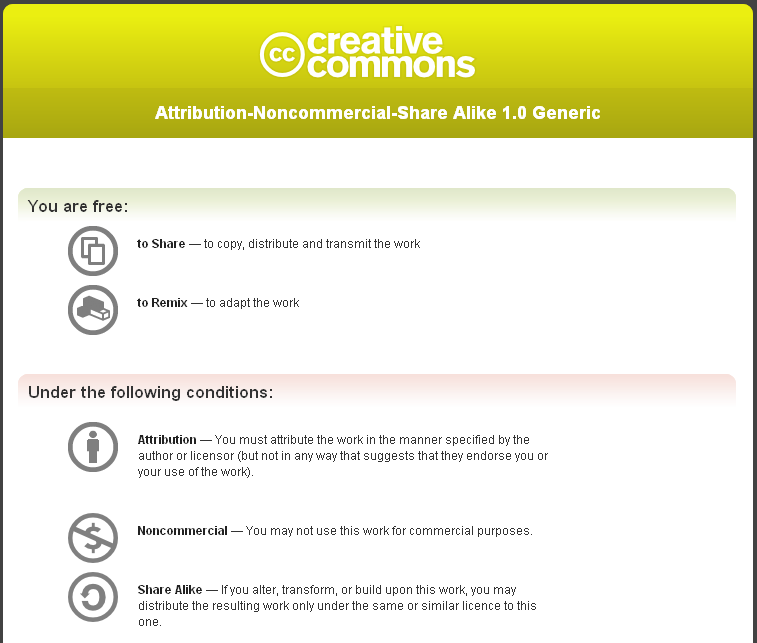
\includegraphics[width=0.74\textwidth]
		{pics/creative_common.png}
	\caption{\license}
	\label{fig:lisensi}
\end{figure}

\pic~\ref{fig:lisensi} diambil dari 
\url{http://creativecommons.org/licenses/by-nc-sa/1.0/deed.en_CA}. 
Jika ingin mengentahui lebih lengkap mengenai \license, silahkan buka 
\url{http://creativecommons.org/licenses/by-nc-sa/1.0/legalcode}. 
Seluruh dokumen yang dibuat dengan menggunakan template ini sepenuhnya 
menjadi hak milik pembuat dokumen dan bebas didistribusikan sesuai dengan 
keperluan masing-masing. 
Lisensi hanya berlaku jika ada orang yang membuat template baru dengan 
menggunakan template ini sebagai dasarnya. 

Dokumen ini dibuat dengan \latex~juga. Untuk meyakinkan Anda, coba lihat 
properti dari dokumen ini dan Anda akan menemukan bagian seperti 
\pic~\ref{fig:pdflatex}. 
Dokumen ini dimaksudkan untuk memberikan gambaran kepada Anda seperti apa 
mudahnya menggunakan \latex~dan juga memperlihatkan betapa bagus dokumen 
yang dihasilkan. 
Seluruh url yang Anda temukan dapat Anda klik. 
Seluruh referensi yang ada juga dapat diklik. 
Untuk mengerti template yang disediakan, Anda tetap harus membuka kode 
\latex~dan bermain-main dengannya. 
Penjelasan dalam PDF ini masih bersifat gambaran dan tidak begitu 
mendetail, dapat dianggap sebagai pengantar singkat. 
Jika Anda merasa kesulitan dengan template ini, mungkin ada baiknya 
Anda belajar sedikit dasar-dasar \latex. 

\begin{figure}
	\centering
	
\includegraphics[width=0.54\textwidth]
		{pics/mark.png}
	\caption{Dokumen Dibuat dengan PDFLatex}
	\label{fig:pdflatex}
\end{figure}

Semoga template ini dapat membantu orang-orang yang ingin mencoba menggunakan 
\latex. Semoga template ini juga tidak berhenti disini dengan ada kontribusi 
dari para penggunanya. 
Kami juga ingin berterima kasih kepada Andreas Febrian, Lia Sadita, Fahrurrozi 
Rahman, Andre Tampubolon, dan Erik Dominikus atas kontribusinya dalam template 
ini. 

\vspace*{0.1cm}
\begin{flushright}
Bandung, XX Januari 2016\\[0.1cm]
\vspace*{1cm}
\penulis

\end{flushright}
%
%
\addChapter{LEMBAR PERSETUJUAN PUBLIKASI ILMIAH}
% 
% @author  Andre Tampubolon, Andreas Febrian
% @version 1.01
% 

\chapter*{\uppercase{Halaman Pernyataan Persetujuan Publikasi Tugas Akhir untuk Kepentingan Akademis}}

\vspace*{0.2cm}
\noindent 
Sebagai sivitas akademik Universitas Indonesia, saya yang bertanda 
tangan di bawah ini:
\vspace*{0.4cm}


\begin{tabular}{p{4.2cm} l p{6cm}}
	\bo{Nama} & : & \penulis \\ 	
	\bo{NPM} & : & \npm \\
	\bo{Program Studi} & : & \program\\	
	\bo{Fakultas} & : & \fakultas\\
	\bo{Jenis Karya} & : & \type \\
\end{tabular}

\vspace*{0.6cm}
\noindent demi pengembangan ilmu pengetahuan, menyetujui untuk memberikan 
kepada Universitas Indonesia \bo{Hak Bebas Royalti Noneksklusif 
(Non-exclusive Royalty Free Right)} atas karya ilmiah saya yang berjudul:
\begin{center}
	\judul
\end{center}
beserta perangkat yang ada (jika diperlukan). Dengan Hak Bebas Royalti 
Noneksklusif ini Universitas Indonesia berhak menyimpan, 
mengalihmedia/formatkan, mengelola dalam bentuk pangkalan data 
(database), merawat, dan memublikasikan tugas akhir saya selama 
tetap mencantumkan nama saya sebagai penulis/pencipta dan sebagai 
pemilik Hak Cipta. \\

\noindent Demikian pernyatan ini saya buat dengan sebenarnya.

\begin{center}
	\vspace*{0.8cm}
	\begin{tabular}{lll}
		Dibuat di&: & Bandung \\
		Pada tanggal&: & \tanggalPengesahan \\
	\end{tabular}\\

	\vspace*{0.2cm}
	Yang menyatakan \\
	\vspace*{1.1cm}
	(\penulis)
\end{center}

\newpage


%
% 
\addChapter{ABSTRAK}
%
% Halaman Abstrak
%
% @author  Andreas Febrian
% @version 1.00
%

\chapter*{Abstrak}

\vspace*{0.2cm}

\begin{center}
	{\large \textbf{PERANCANGAN SISTEM REKOMENDASI LOKASI PENCACAHAN SECARA \textit{REAL-TIME} BERBASIS KONTEKS}} \\
	\vspace*{0.2cm}
	Oleh \\
	{\large \textbf{Aris Prawisudatama}} \\
	{\large \textbf{NIM: 23215131}} \\
	{\large \textbf{(Program Studi Magister Teknik Elektro)}}
\end{center}


\vspace*{0.5cm}

\noindent Pengumpulan data lapangan merupakan salah satu tugas dan kewenangan yang dimiliki oleh institusi statistik sebuah negara, tidak terkecuali Badan Pusat Statistik (BPS). Pada praktiknya, BPS menggunakan Blok Sensus (BS) yang merupakan wilayah kerja dari seorang petugas pencacahan. Pengalokasian wilayah kerja seringkali dilakukan secara subyektif, sehingga menimbulkan ketimpangan waktu penyelesaian antar petugas pencacahan, yang pada akhirnya menyebabkan keterlambatan kegiatan pengumpulan data secara keseluruhan. Walaupun permasalahan alokasi petugas pengumpulan data memiliki kemiripan dengan permasalahan \textit{Multi Depot Vehicle Routing Problem} (VRP), algoritma penyelesaian MDVRP tidak serta merta dapat digunakan, karena informasi terkait lama pencacahan pada suatu wilayah kerja tidak tersedia. \\

\noindent Pada penelitian ini diusulkan sebuah sistem yang dapat digunakan untuk membuat rekomendasi yang lebih merata. Sistem usulan bekerja secara bertahap, dengan menggabungkan algoritma penyelesaian MDVRP dengan mekanisme \textit{Publish/Subscribe}. Agar rekomendasi yang dibuat oleh sistem akurat, digunakan konteks dari setiap petugas pada saat pencarian solusi. \\

\noindent Pengujian dilakukan dengan membandingkan sistem usulan dengan program pembanding, yaitu algoritma MDVRP tanpa menggunakan mekanisme Publish/Subscribe. Berdasarkan hasil pengujian, sistem usulan dapat memberikan rekomendasi dengan lebih efisien pada sebagaian besar kasus.  \\

\vspace*{0.2cm}

\noindent Kata Kunci: rekomendasi; \textit{location routing}; VRP; MDVRP; \textit{publish/subscribe} \\

\newpage
%
%
\addChapter{ABSTRACT}
%
% Halaman Abstract
%
% @author  Andreas Febrian
% @version 1.00
%

\chapter*{ABSTRACT}

\vspace*{0.2cm}

\noindent \begin{tabular}{l l p{11.0cm}}
	Name&: & \penulis \\
	Program&: & \program \\
	Title&: & \judulInggris \\
\end{tabular} \\ 

\vspace*{0.5cm}

\noindent \todo{Write your abstract here.}\\

\vspace*{0.2cm}

\noindent Keywords: \\ 
\noindent \todo{Write up keywords about your report here.}

\newpage

%
% Daftar isi, gambar, dan tabel
%
\tableofcontents
\clearpage
\listoffigures
\clearpage
\listoftables
\clearpage
\listoflistings
\clearpage

%
% Gunakan penomeran Arab (1, 2, 3, ...) setelah bagian ini.
%
\pagenumbering{arabic}

%
%
%
%-----------------------------------------------------------------------------%
\chapter{\babSatu}
%-----------------------------------------------------------------------------%

\section{Latar Belakang}

Badan Pusat Statistik (BPS) merupakan suatu lembaga pemerintah non-departemen yang bertanggung jawab dalam penyediaan statistik dasar \citep{bps_badan_2016}. Dalam peranannya sebagai penyedia data, BPS melakukan pengumpulan data dengan 2 (dua) metode, yaitu primer dan sekunder. Pengumpulan data primer adalah pengumpulan data dengan menggunakan metode wawancara langsung dengan responden, baik responden individu, rumah tangga, maupun perusahaan. Sementara pengumpulan data sekunder adalah pengumpulan data dengan memanfaatkan data yang telah dikumpulkan oleh pihak lain.


Pada pengumpulan data primer oleh BPS, selanjutnya disebut dengan pencacahan, suatu wilayah administratif dibagi dalam beberapa Blok Sensus (BS). Blok sensus merupakan wilayah kerja dari seorang pencacah \citep{bps_sistem_2016}. Setiap petugas pengumpulan data, disebut dengan pencacah, akan dialokasikan dalam beberapa blok sensus yang akan menjadi tanggung jawabnya. Pencacah kemudian akan mendatangi blok sensus tersebut dan mengunjugi setiap rumah tangga yang menjadi sampel pencacahan.


\begin{figure}[h]
    \centering
    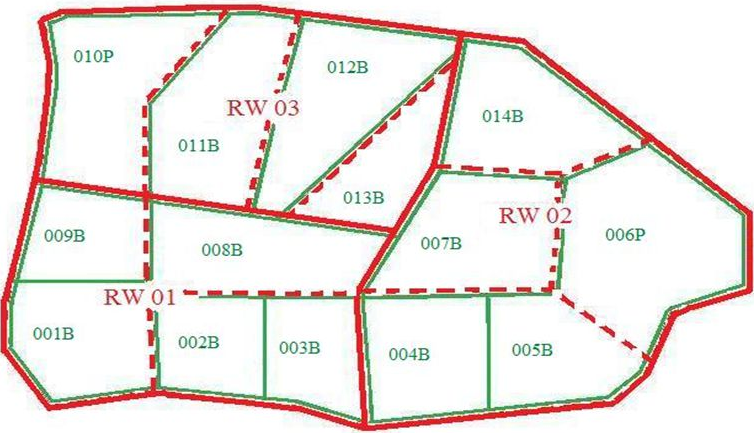
\includegraphics[width=10cm]{../../Resources/Images/peta_kelurahan_per_bs}
    \caption{Pembagian Blok Sensus dalam Desa/Kelurahan}
    \label{fig:capi-ilustration}
\end{figure}


Pengalokasian pencacah terhadap blok sensus terkadang menjadi sesuatu yang sulit, karena terkait dengan waktu dan biaya. \textit{Subject matter} yang menangani kegiatan harus mempertimbangkan beberapa hal, salah satunya adalah jarak antar blok sensus yang menjadi wilayah kerja seorang pencacah. Kesalahan dalam pengalokasian blok sensus menyebabkan waktu pencacahan menjadi lama, yang dapat mempengaruhi kegiatan pencacahan secara keseluruhan.


Selain jarak antar blok sensus, faktor yang juga perlu diperhatikan adalah lamanya pencacahan dalam sebuah blok sensus. Lama pencacahan dalam blok sensus secara umum dipengaruhi oleh 2 (dua) faktor, jarak antar rumah tangga dalam suatu blok sensus dan lama wawancara dalam rumah tangga. \citep{sudman_time_1965}, dalam penelitiannya menyatakan bahwa mengunjungi sebuah segmen dapat menghabiskan 21 persen dari keseluruhan waktu, 15 persen untuk mengunjungi rumah tangga dalam sebuah segmen, 37 persen untuk wawancara, dan sisanya untuk kegiatan lain, seperti \textit{editing}, \textit{study}, dan \textit{clerical}.


Faktor-faktor yang terkait dengan alokasi blok sensus dan petugas tersebut diatas, seperti: jarak antar blok sensus, jarak antar rumah tangga, dan lama wawancara tidaklah selalu tersedia. Andaikan tersedia, datanya-pun bersifat relatif, seperti lama wawancara yang sangat tergantung pada kemampuan pencacah dalam bertanya dan menggali jawaban, tingkat pendidikan responden, dan banyaknya anggota rumah tangga yang harus didata. Oleh karena itu diperlukan suatu cara atau metode yang memungkinkan pengalokasian petugas terhadap blok sensus secara dinamis sesuai dengan context.


Dalam sistem komputer tidak terdapat definisi \textit{context} yang tunggal. Meskipun demikian, sebagian besar definisi sepakat bahwasannya \textit{context} adalah sesuatu yang harus dilakukan terkait interaksi pengguna dan sistem komputer \citep{chen_survey_2000}. \citep{schilit_context-aware_1994}, misalnya, membagi \textit{context} menjadi 4 (empat): \textit{computing context}, \textit{user context}, \textit{physical context}, dan \textit{time context}. \textit{Computing context} meliputi: \textit{network connectivity}, \textit{communication cost}, \textit{communication bandwidth}, dan \textit{nearby resource}; \textit{user context} meliputi: \textit{user profile}, \textit{location}, dan \textit{social situation}; \textit{physical context} meliputi: \textit{lighting}, \textit{noise}, \textit{traffic condition}, dan \textit{temperature}; serta \textit{time context} meliputi: \textit{time of a day}, \textit{week}, \textit{month} and \textit{season of the year}. Senada dengan \citep{schilit_context-aware_1994}, \citep{schmidt_there_1999} mendefinisikan \textit{context} sebagai pengetahuan tentang \textit{state} dari \textit{user} dan \textit{IT device}, termasuk lingkungan, situasi, dan lokasi. Sementara \citep{abowd_towards_1999} mendefinisikan \textit{context} sebagai segala informasi yang dapat digunakan untuk mengkarakterisasi kondisi dari suatu entitas. Entitas yang dimaksud dapat berupa manusia, tempat atau obyek yang relevan dengan aplikasi dan pengguna, termasuk aplikasi dan pengguna itu sendiri. 


\begin{figure}[h]
    \centering
    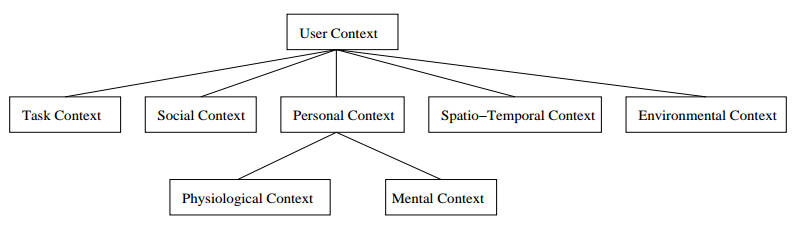
\includegraphics[width=\textwidth]{../../Resources/Images/context}
    \caption{Context Hierarchy \citep{kofod-petersen_case-based_2003}}
    \label{fig:capi-ilustration}
\end{figure}


\textit{Context-aware application} telah banyak digunakan di berbagai bidang. \citep{tsai_context-aware_2016} misalnya, menggunakan \textit{context} untuk menciptakan \textit{smart home environment}. \citep{magara_mplist:_2016} menggabungkan beberapa \textit{context} seperti: lokasi dan aktivitas pengguna, preferensi, label, dan \textit{tags} untuk membuat rekomendasi musik yang akan diputar. Sementara \citep{said_introduction_2013} menciptakan rekomendasi film berdasarkan \textit{time}, \textit{mood}, dan \textit{social recommendation}.


Pada aplikasi yang bersifat \textit{mobile}, \textit{context} biasanya diperoleh dengan menggunakan sensor yang tersemat dalam \textit{mobile device} tersebut. Sekarang ini, telah banyak ditemui \textit{mobile device}, terutama \textit{programmable smartphone}, yang telah dilengkapi dengan berbagai sensor \citep{cao_mobile_2015}. \citep{do_groupus:_2011}, misalnya mem-\textit{propose} GroupUs, framework yang mengelompokkan pengguna berdasarkan aktifitas sehari-hari yang dikumpulkan dengan menggunakan \textit{proximity sensor}. \citep{dai_mobile_2010} menciptakan \textit{drunk driving detection} dengan memanfaatkan sensor \textit{accelerometer} yang tersemat dalam \textit{smartphone}. Sementara \citep{zou_context-aware_2016}, memanfaatkan sensor \textit{Global Posisioning System} (GPS) dan \textit{Micro-Electro-Mechanical System} (MEMS) untuk membuat rekomendasi transportasi. Begitu pula sensor-sensor yang lain juga telah dimanfaatkan dalam berbagai penelitian \citep{dai_perfalld:_2010, lu_soundsense:_2009, bao_movi:_2010, rubel_toward_2005, atzmueller_towards_2013}.


Di sisi yang lain, \textit{location recommendation} merupakan sebuah bahasan yang juga banyak diteliti. Metode yang banyak digunakan untuk menentukan rekomendasi lokasi adalah \textit{Location-based Social Network} (LBSN). Cara kerja LBSN pada dasarnya adalah dengan memanfaatkan lokasi dan \textit{point of interest} yang dibagikan oleh pengguna \citep{yuan_location_2016}. Beberapa peneliti juga mencoba meningkatkan akurasi prediksi dengan menggabungkannya dengan berbagai metode. Misalnya \citep{koren_collaborative_2010}, menggunakan \textit{temporal factorization model} yang memberikan hasil lebih baik dibanding dengan \textit{non-temporal factorization model}. Sementara  \citep{pragarauskas_temporal_2010} mengadopsi \textit{bayesian probabilistic tensor factorization} untuk mewujudkan \textit{temporal collaborative filtering}. Akan tetapi, metode LBSN tidak sesuai digunakan untuk membuat rekomendasi lokasi pencacahan. Hal ini dikarenakan metode LBSN menggunakan \textit{logs} yang telah dikumpulkan sebelumnya, baik \textit{location logs} maupun \textit{user preference logs}, untuk menentukan rekomendasi, sementara lokasi pencacahan bukan merupakan \textit{point of interest} yang dikunjungi oleh banyak orang.


Metode lain yang juga banyak digunakan adalah \textit{Travelling Salesman Problem} (TSP). TSP adalah sebuah algoritma klasik \citep{biggs_graph_1976} yang telah banyak diadopsi dan dimodifikasi. Masalah yang umumnya mejadi dasar modifikasi adalah penggunaan \textit{multiple salesman}, yang disebut dengan \textit{Multiple Travelling Salesman Problem} (MTSP) \citep{bektas_multiple_2006}. Variasi dari MTSP juga telah banyak diteliti, yang umumnya mencakup: \textit{single or multiple depots} (\textit{start and stop point}), jumlah \textit{salesman}, \textit{fixed charges} (jika jumlah \textit{salesman} tidak tetap), lama kunjungan (\textit{time window}), dan \textit{special restrictions} \citep{bektas_multiple_2006}. Berbagai aplikasi untuk menyelesaikan permasalahan nyata (\textit{real-life problem}) juga telah dikembangkan dengan menggunakan MTSP. Misalnya, \textit{print press scheduling} oleh \citep{gorenstein_printing_1970}, \textit{crew scheduling} oleh \citep{svestka_computational_1973}, \textit{school bus routing problem} oleh \citep{angel_computer-assisted_1972}, \textit{interview scheduling} oleh \citep{gilbert_new_1992}, \textit{mission planning} oleh \citep{brumitt_dynamic_1996}, \textit{hot rolling scheduling} oleh \citep{tang_multiple_2000}, dan \textit{global navigation satellite system surveying networks} oleh \citep{saleh_design_2004}.


\begin{figure}[h]
    \centering
    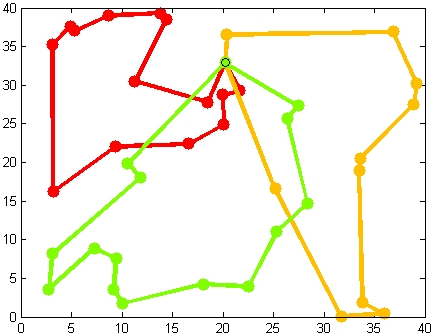
\includegraphics[width=10cm]{../../Resources/Images/mtsp}
    \caption{Ilustrasi \textit{Multiple Travelling Salesman Problem}}
    \label{fig:mtsp-ilustration}
\end{figure}


Asumsi yang digunakan dalam pendekatan MTSP adalah semua informasi telah tersedia pada saat perancangan, sehingga rekomendasi \textit{path} telah diperoleh sebelum kunjungan pertama. Sementara dalam pencacahan, informasi tidak selalu tersedia. Misalnya \textit{service-time}, yang tersusun atas jarak antar rumah tangga dan lama wawancara, merupakan variabel yang bersifat dinamis. Jarak antar rumah tangga sangat tergantung dari sampel yang terpilih, sementara lama wawancara sangat tergantung dari beberapa faktor, seperti: kemampuan pencacah dalam bertanya dan menggali jawaban, kemampuan responden dalam mencerna pertanyaan pencacah, dan banyaknya anggota rumah tangga yang harus didata. Untuk itu, diperlukan suatu metode agar implementasi MTSP untuk rekomendasi lokasi pencacahan dapat mengakomodir \textit{service-time} secara dinamis.


Solusi yang ditawarkan adalah dengan mengabaikan \textit{service-time}, kemudian meng-\textit{generate} rekomendasi baru setiap kali pencacah telah menyelesaikan pencacahan pada suatu blok sensus. Untuk itu, pendekatan MTSP ini akan digabung dengan metode \textit{Publish/Subsribe}. Publish/Subsribe atau pub/sub adalah paradigma dimana \textit{user} mengekspresikan ketertarikan-nya (\textit{subscriptions}), dan agen menerbitkan beberapa penawaran-nya (\textit{event}) \citep{fabret_filtering_2001}. Metode pub/sub yang akan digunakan adalah pub/sub \textit{location-based tracking service}, sebagaimana diusulkan oleh \citep{chen_efficient_2003}.


\section{Rumusan Masalah}

Berdasarkan latar belakang permasalahan yang telah diuraikan sebelumnya, dan didasari motivasi untuk menciptakan rekomendasi alokasi pencacah dan blok sensus secara dinamis, maka dapat dirumuskan masalah dalam penelitian ini adalah bagaimana merancang sebuah sistem rekomendasi lokasi pencacahan dengan memanfaatkan \textit{context} dari pencacah.


Adapun detail dari permasalahan yang akan dikaji adalah sebagai berikut:

\begin{itemize}
\item Bagaimana menentukan \textit{context} apa saja yang dapat digunakan dalam kasus ini.
\item Bagaimana membuat rekomendasi lokasi pencacahan pada kondisi \textit{time windows} sangat berpengaruh, tetapi data tidak tersedia.
\item Bagaimana membuat \textit{conflict resolution}, agar dua atau lebih \textit{smartphone} tidak merekomendasikan lokasi yang sama.
\end{itemize}


\section{Tujuan Penelitian}

Berdasarkan rumusan masalah diatas, maka dapat ditentukan tujuan utama dari penelitian ini adalah untuk menciptakan sebuah sistem rekomendasi lokasi pencacahan secara dinamis. 

Adapun tujuan khusus dari penelitian ini adalah:

\begin{itemize}
\item Mengidentifikasi \textit{context} yang terkait dengan penentuan lokasi pencacahan.
\item Menyusun algoritma rekomendasi.
\item Menyusun algoritma \textit{location conflict}.
\item Mengimplementasikan algoritma usulan dalam \textit{mobile application}.
\item Melakukan ujicoba algoritma dan aplikasi usulan.
\end{itemize}


\section{Batasan Masalah}

Masalah dalam penelitian ini memiliki batasan sebagai berikut:

\begin{itemize}
\item Lokasi pencacahan yang menjadi rujukan adalah Blok Sensus (BS) yang dikeluarkan oleh Badan Pusat Statistik (BPS).
\item \textit{Device} yang digunakan adalah \textit{smartphone} berbasis Android yang umum dijual dipasaran.
\item Tidak mempertimbangkan lingkungan yang tidak terkoneksi dengan jaringan komunikasi.
\end{itemize}


\section{Implikasi}

Manfaat yang dapat diperoleh dari penelitian ini antara lain:


\section{Sistematika Penulisan}

Sistematika penulisan tesis ini terdiri atas enam bab dengan perincian sebagai berikut:

%-----------------------------------------------------------------------------%
\chapter{\babDua}
%-----------------------------------------------------------------------------%


%-----------------------------------------------------------------------------%
\section{\textit{Literature Map}}
\label{sec:literature-map}
%-----------------------------------------------------------------------------%
\textit{Literature Map} merupakan sebuah visualisasi yang memuat \textit{summary} penelitian terkait yang telah dilakukan sebelumnya. \textit{Literature Map} biasanya direpresentasikan dalam sebuah gambar, misalnya menggunakan struktur hierarki \textit{top-down} dalam mempresentasikan literatur \citep{creswell_research_2013}. Ide utama dari penggambaran \textit{literature map} adalah untuk membuat visualisasi dari penelitian terdahulu tentang sebuah topik. 

\begin{figure}[!]
	\centering
	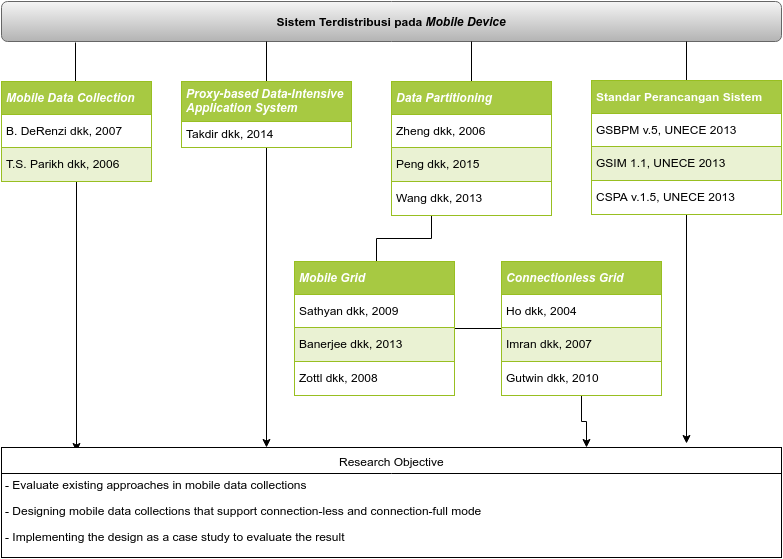
\includegraphics[width=\textwidth]{Resources/Images/literature-map}
	\captionsetup{format=hang}
	\caption{\textit{Literature Map} Penelitian}
	\label{fig:literature-map}
\end{figure}


Berdasarkan review dari literatur yang terkait dengan penelitian ini (\autoref{fig:literature-map}), arsitektur dari rekomendasi lokasi pada pengumpulan data lapangan dapat dibagi menjadi 3 (tiga) kelompok: \textit{context-aware computing}, \textit{location routing}, dan mekanisme komunikasi.


\textit{Context-aware computing} akan membahas beberapa literatur yang berkaitan dengan definisi dari konteks itu sendiri dan pemanfaatannya dalam komputasi. \textit{Location routing} akan membahas literatur terkait beberapa algoritma yang biasa digunakan dalam penyelesaian masalah \textit{location routing}. Sementara mekanisme komunikasi akan mendiskusikan tentang beberapa metode yang dapat digunakan oleh \textit{client} dan \textit{server} dalam berkormunikasi.


%-----------------------------------------------------------------------------%
\section{Badan Pusat Statistik}
\label{sec:badan-pusat-statistik}
%-----------------------------------------------------------------------------%
Badan Pusat Statistik (BPS) adalah Lembaga Pemerintah Non-Departemen yang bertanggung jawab dan memiliki peranan dalam penyediaan data. Berdasarkan Rencana Strategis BPS 2015-2019, BPS memiliki misi yang harus dijalankan yaitu:
\begin{enumerate}
\item Menyediakan data statistik berkualitas melalui kegiatan statistik yang terintegrasi dan berstandar nasional maupun internasional. \\
Dalam rangka menyediakan data berkualitas, data yang dihasilkan BPS harus memenuhi dimensi kualitas yakni relevan, akurat, disajikan tepat waktu, koheren, dapat diakses, dan dapat diinterpretasikan.
\item Memperkuat Sistem Statistik Nasional yang berkesinambungan melalui pembinaan dan koordinasi di bidang statistik.
\item Membangun insan statistik yang profesional, berintegritas dan amanah untuk kemajuan perstatistikan.
Dalam menyelenggarakan kegiatan statistik, insan statistik harus memiliki kapasitas dan kapabilitas yang diperlukan untuk menghasilkan data statistik yang berkualitas.
\end{enumerate}


Di dalam menjalankan peranan sebagai penyedia data, BPS menyelenggarakan statistik dasar dengan cara sensus, survei, dan kompilasi administrasi untuk mendapatkan data. Data yang berkualitas hanya dapat diperoleh melalui proses yang berkualitas pula. Terdapat berbagai variabel yang menjadi parameter proses yang berkualitas, salah satunya adalah ketepatan waktu dalam proses pengumpulan data.

Pengumpulan data merupakan suatu proses yang sangat fleksibel. Ketepatan waktu pengumpulan data sangat rentan terhadap pengaruh berbagai faktor, seperti kualitas petugas pengumpulan data, kualitas responden, jumlah anggota rumah tangga yang didata, jarak antar lokasi pencacahan, jarak antar rumah tangga dalam satu segmen, dan kondisi alam. Alokasi petugas pengumpulan data secara baku yang hanya memperhatikan jumlah lokasi pencacahan dan petugas, tidak dapat mengakomodir faktor-faktor tersebut. Akibatnya, waktu penyelesaian pengumpulan data bisa bervariasi antara satu petugas dengan petugas lainnya. Oleh karena itu, diperlukan suatu metode baru dalam pengalokasian petugas yang dapat mengantisipasi terjadinya kesenjangan beban tugas baik dari segi waktu maupun kuantitas.  

%-----------------------------------------------------------------------------%
\section{\textit{Context-aware Computing}}
\label{sec:context-aware-computing}
%-----------------------------------------------------------------------------%


%-----------------------------------------------------------------------------%
\subsection{Definisi \textit{Context}}
\label{ssec:context-definition}
%-----------------------------------------------------------------------------%
Semenjak \textit{Context-aware computing} pertama kali diperkenalkan oleh \citep{schilit_context-aware_1994}, berbagai definisi mengenai \textit{context} dan \textit{context-awareness} telah berkembang luas. Sebagaian besar definisi yang ada saat ini, menurut \citep{zimmermann_operational_2007}, dapat dikelompokkan menjadi dua: definisi menurut sinonim dan definisi menurut contoh. \textit{Context} mengalami berbagai penggolongan menggunakan sinonim seperti \textit{application environment} \citep{hull_towards_1997} atau situasi \citep{brown_stick-e_1995}. Sementara beberapa authors, seperti \citep{brown_context-aware_1997}, \citep{gross_awareness_2001}, dan \citep{ryan_enhanced_1999}, mendefinisikan \textit{context by example} dan \textit{context element} seperti lokasi, identitas, waktu, suhu, kebisingan sama dengan kepercayaan, keinginan, komitmen, dan hubungan dengan manusia \citep{chen_intelligent_2003}.


Secara umum, dapat dikatakan bahwasanya \textit{context} adalah informasi yang dapat digunakan dalam menjelaskan situasi dari sebuah entitas. Entitas dapat dapat berupa manusia, lokasi, atau obyek yang relevan dengan interaksi antara seorang pengguna dan aplikasi, termasuk pengguna dan aplikasi itu sendiri \citep{dey_understanding_2001}. \citep{schilit_context-aware_1994} menyebutkan bahwa yang termasuk ke dalam \textit{context} adalah: lokasi dari penggunaan, kumpulan orang-orang sekitar, \textit{hosts}, dan \textit{accessible devices}, serta perubahan hal-hal tersebut dari waktu ke waktu. \citep{dey_understanding_2001} mengembangkan definisi dari \citep{schilit_context-aware_1994} dengan menyatakan "\textit{Context} adalah lokasi, identitas dan status dari individu, kelompok, dan obyek komputasi".


%-----------------------------------------------------------------------------%
\subsection{Kategori \textit{Context}}
\label{ssec:context-category}
%-----------------------------------------------------------------------------%
Dari berbagai informasi yang menjelaskan entitas dari \textit{context}, semuanya mengarah ke 5 (lima) kategori, yaitu: \textit{individuality}, aktivitas, lokasi, waktu, dan relasi, seperti pada Gambar \ref{fig:context-categories} \citep{zimmermann_operational_2007}. Kategori \textit{individuality} memuat properti dan atribut yang menjelaskan entitas itu sendiri. Kategori aktivitas mencakup seluruh kegiatan yang dilakukan entitas tersebut. Kategori lokasi dan waktu menyediakan koordinat \textit{spatio-temporal} dari entitas. Sementara kategori relasi merepresentasikan informasi tentang hubungan antara sebuah entitas dengan entitas yang lain.


\begin{figure}[!]
	\centering
	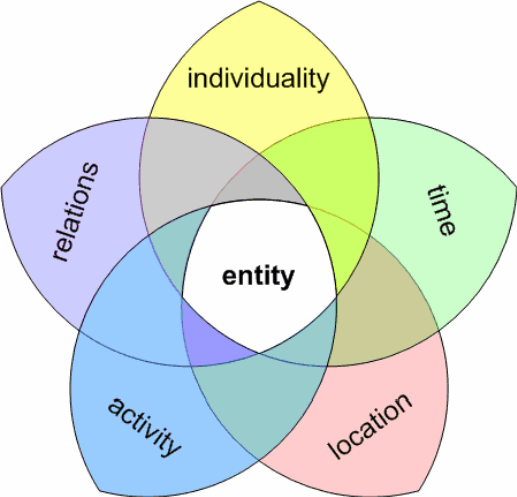
\includegraphics[width=6cm]{Resources/Images/context-categories}
	\captionsetup{format=hang}
	\caption{Kategori dari \textit{Context}}
	\label{fig:context-categories}
\end{figure}


%-----------------------------------------------------------------------------%
\subsubsection{\textit{Individuality Context}}
\label{sssec:individuality-context}
%-----------------------------------------------------------------------------%
Kategori ini memberi akses kepada informasi yang bersifat kontekstual tentang entitas terkait. Informasi ini dapat berupa apa saja terkait entitas tersebut, tetapi umumnya adalah \textit{state} dari entitas. Entitas dapat berupa entitas individu atau sekelompok entitas yang saling berbagi \textit{context} yang terkait. Entitas dapat berupa entitas yang \textit{real} (eksis secara nyata), maupun virtual (hanya terdapat di lingkup informasi). Selain itu, terdapat juga entitas yang bersifat \textit{mobile}, \textit{movable}, maupun \textit{fixed}. kategori \textit{inviduality context} dikelompokkan menjadi empat, yaitu: \textit{natural}, \textit{human}, \textit{artificial}, dan \textit{group entities}.


%-----------------------------------------------------------------------------%
\subsubsection{\textit{Time Context}}
\label{sssec:time-context}
%-----------------------------------------------------------------------------%
Waktu merupakan aspek yang vital dalam klasifikasi \textit{context}, karena sebagian besar pernyataan sangat terkait dengan dimensi \textit{temporal}. Kategori ini menkalkulasi informasi seperti \textit{time zone} dari \textit{client}, dan \textit{current time} atau \textit{virtual time}. Contoh representasi dari waktu adalah \textit{time zone}, misalnya format \textit{ Central European Time (CET)}, yang menyediakan fasilitas kalkulasi secara matematis dan komparasi waktu. Model dimensi waktu yang sering diimplementasikan dalam \textit{context-aware computing} misalnya jam kerja atau hari libur.


\textit{Context} yang disimpan secara persisten dapat membentuk sebuah \textit{data pool} yang berisi histori dari informasi terkait \textit{context} tersebut. Histori tersebut membentuk basis data untuk \textit{context information} dari event yang telah lampau. Basis data yang dipersistenkan dapa digunakan sebagai bahan analisis dari kebiasaan dari pengguna dan prediksi.


%-----------------------------------------------------------------------------%
\subsubsection{\textit{Location Context}}
\label{sssec:location-context}
%-----------------------------------------------------------------------------%
Dengan semakin berkembangnya \textit{portable/mobile devices}, lokasi menjadi parameter yang penting dalam \textit{context-aware system}. Obyek-obyek fisik dan perangkat tersusun secara spasial, dipengaruhi oleh pergerakan pengguna. Kategori ini berisi model lokasi yang terklasifikasi secara fisik maupun virtual, misalnya \textit{IP address} sebagai posisi komputer dalam sebuah jaringan, koordinat, maupun informasi spasial terkait seperti kecepatan dan orientasi. Lokasi dapat berupa lokasi absolut atau lokasi relatf, yaitu lokasi yang diperhitungkan dari objek yang lain. Model dapat juga terdiri dari lokasi kuantitatif (geometrik) dan kualitatif (simbol).


Lokasi yang bersifat kuantitatif merujuk kepada koordinat dengan dua dimensi, tiga dimensi, atau lebih. Sebagai contoh, koordinat dua dimensi secara geografis melambangkan setiap lokasi di bumi secara lintang dan bujur. Informasi terkait koordinat geografis biasanya diperoleh melalui \textit{Global Posisitioning System} dengan menggunakan satelit. Selain itu, lokasi juga dapat diklasifikasikan menjadi dalam dan luar ruangan, sinyal radio atau cahaya, dll. Sementara itu, lokasi yang bersifat kualitatif dan berupa bangunan, ruangan, jalan, negara, dan sebagainya. 


%-----------------------------------------------------------------------------%
\subsubsection{\textit{Activity Context}}
\label{sssec:activity-context}
%-----------------------------------------------------------------------------%
\textit{Context} aktivitas meliputi aktivitas yang sedang dikerjakan oleh sebuah entitas. Kategori ini dapat diterjemahkan menjadi: tujuan, kegiatan, dan aksi. Sebuah \textit{task} merupakan aktivitas yang berorientasi pada capaian. Capaian atau \textit{goals} dapat bersifat \textit{low-level}, dimana \textit{goal} dapat sering berganti, atau \textit{high-level}, dimana \textit{goal} bersifat konsisten.


%-----------------------------------------------------------------------------%
\subsubsection{\textit{Relations Context}}
\label{sssec:relations-context}
%-----------------------------------------------------------------------------%
Kategori ini mencakup relasi dari sebuah entitas yang berhubungan dengan entitas yang lain. Entitas yang lain tersebut dapat berupa manusia, benda, layanan, atau informasi (misalnya teks, gambar, film, suara). Karakteristik dari \textit{environment} biasanya dibangun secara spasial dan temporal. Individu dalam kelompok saling mempengaruhi kelompok dalam satu relasi, misalnya seluruh manusia dengan umur yang sama.


%-----------------------------------------------------------------------------%
\subsection{\textit{Context-aware Computing}}
\label{ssec:context-aware-computing}
%-----------------------------------------------------------------------------%
\citep{dey_understanding_2001} menjelaskan, sebuah sistem dikatakan \textit{context-aware} jika dia menggunakan \textit{context} untuk menyediakan informasi atau layanan yang relevan kepada pengguna, dimana relevansinya tergantung dari apa yang pengguna kerjakan.


Terdapat berbagai contoh sistem yang bersifat \textit{context-aware}. \citep{tsai_context-aware_2016} misalnya, menggunakan \textit{context} untuk menciptakan \textit{smart home environment}. \citep{magara_mplist:_2016} menggabungkan beberapa \textit{context} seperti: lokasi dan aktivitas pengguna, preferensi, label, dan \textit{tags} untuk membuat rekomendasi musik yang akan diputar. Sementara \citep{said_introduction_2013} menciptakan rekomendasi film berdasarkan \textit{time}, \textit{mood}, dan \textit{social recommendation}.


Pada aplikasi yang bersifat \textit{mobile}, \textit{context} biasanya diperoleh dengan menggunakan sensor yang tersemat dalam \textit{mobile device} tersebut. Sekarang ini, telah banyak ditemui \textit{mobile device}, terutama \textit{programmable smartphone}, yang telah dilengkapi dengan berbagai sensor \citep{cao_mobile_2015}. \citep{do_groupus:_2011}, misalnya mem-\textit{propose} GroupUs, framework yang mengelompokkan pengguna berdasarkan aktivitas sehari-hari yang dikumpulkan dengan menggunakan \textit{proximity sensor}. \citep{dai_mobile_2010} menciptakan \textit{drunk driving detection} dengan memanfaatkan sensor \textit{accelerometer} yang tersemat dalam \textit{smartphone}. Sementara \citep{zou_context-aware_2016}, memanfaatkan sensor \textit{Global Posisioning System} (GPS) dan \textit{Micro-Electro-Mechanical System} (MEMS) untuk membuat rekomendasi transportasi. Begitu pula sensor-sensor yang lain juga telah dimanfaatkan dalam berbagai penelitian \citep{dai_perfalld:_2010, lu_soundsense:_2009, bao_movi:_2010, rubel_toward_2005, atzmueller_towards_2013}.


Pada kasus yang dijadikan dasar dari penelitian ini, yaitu terkait pengumpulan data lapangan, \textit{context} yang akan digunakan adalah \textit{spatio-temporal context}, yang meliputi lokasi dan waktu dari setiap pencacah.


%-----------------------------------------------------------------------------%
\section{\textit{Location Routing}}
\label{sec:location-routing}
%-----------------------------------------------------------------------------%
\textit{Location routing problem} (LRP), menurut \citep{nagy_location-routing:_2007}, secara umum dapat dikatakan sebagai sebuah pendekatan dalam pemodelan dan penyelesaian permasalahan terkait lokasi. Definisi ini mengikuti konsep dari \citep{bruns_zweistufige_1998}, yaitu perencanaan lokasi yang mempertimbangkan perencanaan \textit{tour}. Definisi ini juga senada dengan \citep{balakrishnan_integrated_1987}, yang menyatakan bahwa \textit{location routing problem} merupakan keputusan strategis yang berfokus pada lokasi fasilitas.


Lokasi dari fasilitas dan \textit{vehicle routing} merupakan area yang saling terkait. \citep{maranzana_location_1964} menyatakan bahwa "\textit{the location of factories, warehouses and supply points in general...is often influenced by transport costs."}. Tetapi beberapa peneliti, sebagaimana \citep{nagy_location-routing:_2007}, menolak korelasi tersebut dengan beberapa alasan:

\begin{enumerate}
\item Terdapat beberapa kondisi dimana \textit{location problem} tidak memiliki aspek \textit{routing}, 
\item Permasalah lokasi bersifat strategis, sementara permasalahan \textit{routing} bersifat taktis. Rute dapat dikalkukasi dan diputuskan secara berkala (bahkan terkadang harian).
\end{enumerate}


\textit{Location Routing Problem} meliputi topik bahasan yang luas. Menurut \citep{nagy_location-routing:_2007}, LRP setidaknya dapat dikelompokkan dalam 4 (empat) klasifikasi:

\begin{enumerate}
\item Berdasarkan struktur hierarkinya.\\
	Sebagian besar LRP terdiri dari beberapa fasilitas yang melayani sejumlah \textit{customer}, yang terhubung dengan masing-masing depot berdasarkan \textit{tour}. Akan tetapi, ada beberapa struktur LRP yang tidak standar, antara lain: 
	\begin{enumerate}
	\item \textit{transportation-location problem} tidak melibatkan perencanaan \textit{tour}, 
	\item \textit{many-to-many routing problem}, yang selain melibatkan perencaan \textit{tour} antara fasilitas-\textit{customer}, juga melibatkan rute antara fasilitas, 
	\item \textit{vehicle routing-allocation problem} menyertakan rencana \textit{tour} antar fasilitas, tetapi tidak antara fasilitas dan \textit{customer}, 
	\item \textit{multi-level location-routing problem} mengikutsertakan rencana \textit{tour} untuk kedua \textit{layer}, dan bahkan mungkin lebih dari satu level fasilitas.
	\end{enumerate}
\item Tipe input data. \\
	Terdapat dua macam tipe input data: \textit{deterministic} dan \textit{stochastic}. Sebagian besar kasus pada LRP bersifat \textit{deterministic}. Adapun pada kasus LRP yang bersifat \textit{stochastic}, variabel \textit{stochastic} biasanya hanya terdapat pada \textit{demand}.
\item Periode perencanaan. \\
	Berdasarkan periode perencanaan, terdapat \textit{single-period} dan \textit{muti-depot}. Permasalahan ini juga sering disebut dengan \textit{static} dan \textit{dynamic}. Umumnya, mayoritas penelitian lebih berfokus pada permasalahan \textit{static} LRP.
\item Metode solusi. \\
	Berdasarkan metode solusi, terdapat metode \textit{exact} dan \textit{heuristic}. Sebagian besar peneliti menggunakan metode \textit{exact}, walaupun untuk sebagian kasus, penggunaan metode \textit{exact} lebih sukses.
\end{enumerate}


Sementara itu, berdasarkan strukturnya, LRP juga setidaknya dapat dipecah menjadi lima jenis:
\begin{enumerate}
\item Fungsi objektif. \\
	objektif yang paling umum digunakan dalam permasalahan \textit{location routing} adalah minimal keseluruhan \textit{cost}, dimana \textit{cost} dapat dipecah menjadi \textit{depot cost} dan \textit{vehicle cost}. Hanya terdapat sedikit penelitian yang menggunakan fungsi objektif selain \textit{total overall cost} atau \textit{multiobjective}, antara lain \citep{averbakh_technical_1994} dan \citep{averbakh_probabilistic_1995}.
\item \textit{Solution space}. \\
	Solution space dapat berupa diskrit, kontinyu, atau \textit{network}. Sebagian besar literatur dalam permasalahan LRP menggunakan lokasi yang bersifat diskrit. Akan tetapi ada beberapa permasalahan \textit{round-trip location} yang terbatas pada \textit{path} atau \textit{tree network}, salah satunya \citep{simchi-levi_capacitated_1991}.
\item  Jumlah \textit{depot}. \\
	Berdasarkan jumlah \textit{depot} yang digunakan, terdapat \textit{single depot} dan \textit{multi depot} LRP. Sebagian besar penelitian menggunakan \textit{multi depot}, meskipun ada beberapa kasus yang terbatas hanya pada \textit{single depot}, antara lain \citep{laporte_exact_1981}, \citep{averbakh_technical_1994}, dan \citep{simchi-levi_capacitated_1991}. 
\item Jumlah dan tipe kendaraan. \\
	Pada sebagaian besar penelitian LRP, jumlah kendaraan yang digunakan tidak tetap dan tipe kendaraan bersifat homogen. Meskipun begitu, terdapat juga penelitian yang menggunakan kendaraan yang bertipe heterogen, seperti \citep{bookbinder_vehicle_1988} dan \citep{salhi_intergrated_1996}. Selain itu, terdapat kasus khusus dimana sebuah depot hanya terdapat satu kendaraan, misalnya \citep{branco_hamiltonian_1990}.
\item Struktur rute. \\
	Struktur rute yang biasa dipakai adalah dengan memulai dari sebuah \textit{depot}, kemudian mengunjungi sejumlah \textit{customer}, dan kembali lagi ke \textit{depot} asal. Terdapat pula struktur rute yang memungkinkan adanya \textit{multiple trip}, dan \textit{pickup-delivery}.
\end{enumerate}


%-----------------------------------------------------------------------------%
\subsection{\textit{Vehicle Routing Problem}}
\label{ssec:vrp}
%-----------------------------------------------------------------------------%
\textit{Vehicle Routing Problem} (VRP) merupakan salah satu permasalahan optimasi kombinatorial yang diusulkan pertama kali oleh \citep{dantzig_truck_1959}. VRP dapat dideskripsikan sebagai permasalahan dalam menentukan desain pengiriman yang optimal atau koleksi rute dari satu atau lebih \textit{depot} ke sejumlah kota atau pelanggan (\textit{customer}) yang tersebar secara geografis \citep{laporte_vehicle_1992}. VRP memiliki peran yang penting dalam dalam distribusi logistik. Pada VRP (\autoref{fig:vrp-ilustration}), kunjungan dimulai dengan kendaraan meninggalkan \textit{depot}, melayani sejumlah \textit{customer}, dan kembali lagi ke depot asal, dimana masing-masing \textit{customer} ditandai dengan \textit{demand}. VRP klasik merupakan generalisasi dari \textit{Traveling Salesman Problem} (TSP) dan \textit{Bin Packaging Problem} (BPP) \citep{garey_computers_2002}.


VRP dapat didefinisikan sebagai berikut, $G = (V, A)$ adalah sebuah \textit{graph} dimana $V = {1,...,n}$ adalah sebuah set dari simpul(\textit{vertex}) yang merepresentasikan kota dengan \textit{depot} berada pada vertex $1$. Sementara $A$ merupakan sebuah set dari busur(\textit{arc}), dimana setiap $arc(i, j)$ $i \neq j$ diasosiasikan dengan matrik jarak \textit{non-negative} $C = (c_{ij})$. Dalam beberapa konteks, $c_{ij}$ dapat diinterpretasikan sebagai \textit{travel cost} atau \textit{travel time}. Ketika $C$ bersifat simetris, makan seringkali $A$ diganti dengan satu set $E$ dari \textit{undirected edges}. Sebagai tambahan, jika diasumsikan terdapat $m$ kendaraan yang berada pada depot, dimana $m_L < m < m_U$, maka ketika $m_L = m_U$, maka $m$ dikatakan \textit{fixed}, dan ketika $m_L = 1$ dan $m_U = n - 1$, maka $m$ dikatakan \textit{free}. Jika $m$ tidak \textit{fixed}, maka seringkali diasosiasikan \textit{fixed cost} $f$ untuk setiap kendaraan. Pada VRP klasik, asumsi bahwasannya setiap kendaraan identik dan memiliki kapasitas yang sama, yaitu $D$.


VRP terdiri dari satu set rute dari kendaraan yang memiliki \textit{cost} terkecil, dengan ketentuan:
\begin{enumerate}
\item Setiap \textit{customer} pada $V$ dikunjungi hanya sekali dan oleh satu kendaraan, 
\item Semua kendaraan memulai dan mengakhiri perjalanan pada satu \textit{depot}, 
\item Total \textit{demand} dari seluruh \textit{customer} pada setiap rute tidak melebihi $Q$, 
\item Durasi total dari rute tidak melebihi $D$
\end{enumerate}


\begin{figure}[!]
	\centering
	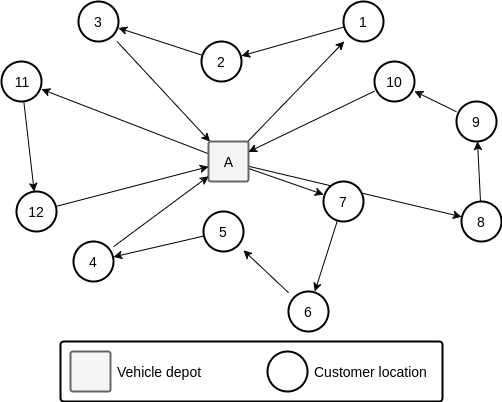
\includegraphics[width=9cm]{Resources/Images/vrp-ilustration}
	\captionsetup{format=hang}
	\caption{Ilustrasi \textit{Vehicle Routing Problem (VRP)}}
	\label{fig:vrp-ilustration}
\end{figure}


Terdapat sejumlah variasi dari VRP klasik yang telah diteliti, antara lain: \textit{Capacitated VRP (CVRP)} yang diteliti oleh \citep{baldacci_exact_2010}, \citep{cordeau_chapter_2007}, dan \citep{toth_vehicle_2002}; \textit{VRP with Time Windows (VRPTW)}, \textit{VRP with Pickup and Delivery (VRPPD)}, dan \textit{Periodic VRP (PVRP)} oleh \citep{solomon_survey_1988}; \textit{Dynamic VRP (DVRP)} oleh \citep{psaraftis_dynamic_1995}, dan berbagai varian lainnya, dimana keseluruhannya hanya mempertimbangkan satu buah depot. Sementara itu, \textit{Multi-Depot Vehicle Routing Problem (MDVRP)} merupakan salah satu varian dari VRP klasik dimana terdapat lebih dari satu \textit{depot} yang digunakan. Gambar \ref{fig:vrp-variants} memberikan ilustrasi hierarki variasi dari VRP.


\begin{figure}[!]
	\centering
	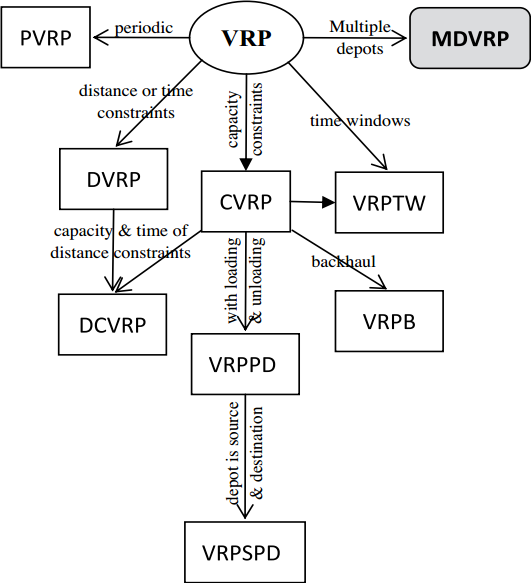
\includegraphics[width=8cm]{Resources/Images/vrp-variants}
	\captionsetup{format=hang}
	\caption{Hierarki variasi dari VRP \citep{weise_solving_2009}}
	\label{fig:vrp-variants}
\end{figure}


%-----------------------------------------------------------------------------%
\subsection{\textit{Multi-Depot Vehicle Routing Problem}}
\label{ssec:mdvrp}
%-----------------------------------------------------------------------------%
\textit{Multi-Depot Vehicle Routing Problem (MDVRP)} merupakan salah satu varian dari VRP klasik dimana terdapat lebih dari satu \textit{depot} yang digunakan. Pada variasi ini, setiap \textit{customer} akan dikunjungi oleh kendaraan yang berasal dari salah satu dari beberapa \textit{depot}. Pada MDVRP standar, kendaraan harus memulai dan mengakhiri rute pada depot yang sama. Gambar \ref{fig:mdvrp-illustration} memberikan ilustrasi tentang MDVRP.


\begin{figure}[!]
	\centering
	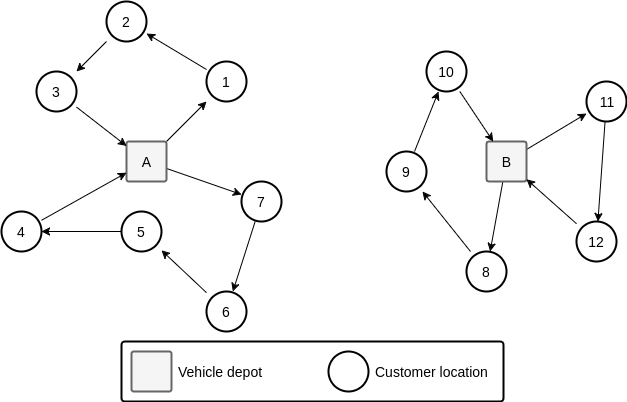
\includegraphics[width=11cm]{Resources/Images/mdvrp-illustration}
	\captionsetup{format=hang}
	\caption{Ilustrasi \textit{Multi Depot} VRP}
	\label{fig:mdvrp-illustration}
\end{figure}


Berdasarkan \citep{renaud_tabu_1996}, MDVRP dapat diformulasikan sebagai berikut, $G = (V, A)$ adalah sebuah \textit{graph}, dimana $V$ adalah sebuah set dari simpul(\textit{vertex} atau \textit{node}) dan $A$ adalah sebuah set dari busur(\textit{arcs}). \textit{Node} dibagi menjadi 2 (dua) \textit{subset}: \textit{customer} yang akan dilayani $V_C$ = \{1,..., $N$\}, dan satu set depot $V_D$ = \{$N$+1,..., $N+M$\}, dimana $V_C \cup V_D$ = $V$ dan $V_C \cap V_D$ = $\oslash$. Terdapat biaya \textit{non-negative} $c_{ij}$ yang diasosiasikan untuk setiap \textit{arc} $(i, j) \in A$. \textit{Demand} untuk masing-masing \textit{customer} adalah $d_i$, dan tidak ada \textit{demand} pada \textit{depot node}. Terdapat juga sejumlah $K$ kendaraan yang identik, yang masing-masing memiliki kapasitas $Q$. \textit{Service time} untuk masing-masing \textit{customer} $i$ adalah $t_i$, sementara waktu durasi maksimum untuk masing-masing rute adalah $T$. Faktor konversi $w_{ij}$ mungkin dibutuhkan untuk menkonversi \textit{cost} $c_{ij}$ menjadi unit waktu. Pada MDVRP klasik, \textit{cost} sama dengan waktu dan unit jarak, sehingga $w_{ij}$ = $1$.


Dalam formula matematika, berdasarkan \citep{kulkarni_integer_1985}, variabel biner $x_{ijk}$ sama dengan $1$ ketika kendaraan $k$ mengunjungi \textit{node} $j$ tepat setelah \textit{node} $i$. Variabel tambahan $y_i$ juga digunakan untuk mengeliminasi \textit{subtour}. Persamaan \ref{eq:1} meminimalisasi \textit{total cost}. Persamaan \ref{eq:2} dan \ref{eq:3} menjamin bahwa setiap \textit{customer} hanya dilayani tepat satu kali oleh satu kendaraan. Alur kendaraan dijamin dengan persamaan \ref{eq:4}. Kapasitas kendaraan dan batasan durasi untuk setiap rute terdapat pada persamaan \ref{eq:5} and \ref{eq:6}. Persamaan \ref{eq:7} dan \ref{eq:8} mengecek keberadaan kendaraan. Eliminasi \textit{subtour} terdapat pada persamaan \ref{eq:9}. Terakhir, persamaan \ref{eq:10} dan \ref{eq:11} mendefinisikan $x$ dan $y$ sebagai variabel biner.


\begin{flalign}
\label{eq:1}
&\sum_{i=1}^{N+M}\sum_{j=1}^{N+M}\sum_{k=1}^{K}c_{ij}x_{ijk};
\end{flalign}


\begin{flalign}
\label{eq:2}
\sum_{i=1}^{N+M}\sum_{k=1}^{K}x_{ijk} = 1  (j=1,..., N);
\end{flalign}


\begin{flalign}
\label{eq:3}
\sum_{j=1}^{N+M}\sum_{k=1}^{K}x_{ijk} = 1  (j=1,..., N);
\end{flalign}


\begin{flalign}
\label{eq:4}
&\sum_{i=1}^{N+M}x_{ihk} - \sum_{j=1}^{N+M}x_{hjk} = 0 \\
\nonumber
&(k=1,...,K; h=1,...,N+M);
\end{flalign}


\begin{flalign}
\label{eq:5}
\sum_{i=1}^{N+M} \sum_{j=1}^{N+M} d_ix_{ijk} \leq Q (k=1,...,K);
\end{flalign}


\begin{flalign}
\label{eq:6}
\sum_{i=1}^{N+M} \sum_{j=1}^{N+M} (c_{ij}w_{ij} + t_i) x_{ijk} \leq T (k=1,...,K);
\end{flalign}


\begin{flalign}
\label{eq:7}
\sum_{i=N+1}^{N+M} \sum_{j=1}^{N} x_{ijk} \leq 1 (k=1,...,K);
\end{flalign}


\begin{flalign}
\label{eq:8}
\sum_{j=N+1}^{N+M} \sum_{i=1}^{N} x_{ijk} \leq 1 (k=1,...,K);
\end{flalign}


\begin{flalign}
\label{eq:9}
&y_i - y_j + (M + N)x_{ijk} \leq N + M - 1; \\
\nonumber
&for 1 \leq i \neq j \leq N and 1 \leq k \leq K;
\end{flalign}


\begin{flalign}
\label{eq:10}
x_{ijk} \in \{0, 1\} \forall i,j,k;
\end{flalign}


\begin{flalign}
\label{eq:11}
y_i \in \{0,1\} \forall i;
\end{flalign}


Terdapat beberapa algoritma yang dapat digunakan untuk menyelesaikan permasalahan MDVRP. \citep{laporte_optimal_1984} dan \citep{laporte_solving_1988} mengembangkan algoritma \textit{branch-and-bound}, tetapi, algoritma ini hanya dapat digunakan untuk sejumlah kecil \textit{instance}. Sejumlah algoritma \textit{heuristic} juga telah diteliti untuk MDVRP. Algoritma heuristic yang relatif awal, yang berbasis pada prosedur \textit{simple construction and improvement} diteliti oleh \citep{tillman_multiple_1969}, \citep{tillman_upperbound_1972}, \citep{tillman_study_1971}, \citep{wren_computer_1972}, \citep{gillett_multi-terminal_1976}, \citep{golden_implementing_1977}, dan \citep{raft_modular_1982}. Penelitian yang lebih baru, \citep{chao_new_1993} mengusulkan sebuah prosedur pencarian yang mengkombinasikan metode lokal \textit{record-to-record} \citep{dueck_new_1993} untuk mengalokasikan ulang pelanggan ke rute kendaraan yang berbeda, yang dilanjutkan dengan prosedur 2-opt \citep{lin_computer_1965} untuk meningkatkan rute individual.


Penelitian yang lain, \citep{renaud_tabu_1996} menggunakan \textit{tabu search heuristic} dimana solusi awal disusun dengan meng-\textit{assign} setiap \textit{customer} dengan depot terdekatnya. Algoritma \textit{petal} yang dirancang oleh penulis yang sama, \citep{renaud_improved_1996}, kemudian digunakan untuk mencari solusi dari setiap VRP yang diasosiasikan pada masing-masing depot. Terakhir terdapat fase \textit{improvement}, baik dengan menggunakan subset dari pertukaran 4-opt untuk meningkatkan rute individual, menukar \textit{customer} antar rute dari depot yang sama maupun berbeda, atau menukar \textit{customer} antara 3 (tiga) rute.


Penggunaan tabu search juga dilakukan oleh \citep{cordeau_tabu_1997}, dimana solusi awal diperoleh dengan meng-assign setiap \textit{customer} dengan depot terdekat dan solusi digenerate untuk masing-masing depot dengan menggunakan algoritma sweep. \textit{Improvement} dilakukan dengan memindahkan \textit{customer} antara dua rute kepada depot yang sama, atau dengan merelokasi \textit{customer} pada rute ke depot yang lain. \textit{Reinsertion} dilakukan dengan menggunakan \textit{GENI heuristic} \citep{gendreau_new_1992}.


Selain tabu search, terdapat juga beberapa algoritma yang dapat digunakan untuk menyelesaikan permasalahan MDVRP, yaitu: adaptive large neighborhood search (ALNS) \citep{pisinger_general_2007}, fuzzy logic guided genetic algorithm (FLGA) \citep{lau_application_2010}, paralel iterated tabu search (ITS) \citep{cordeau_parallel_2012}, hybrid algorithm combining Iterated Local Search and Set Partitioning (ILS-RVND-SP) \citep{subramanian_hybrid_2013}, hybrid genetic algorithm with adaptive diversity control (HGSADC+) \citep{vidal_implicit_2014}, hybrid Granular Tabu Search (ELTG) \citep{escobar_hybrid_2014}, dan evolution algorithms (EAs) \citep{weise_solving_2009}.


%-----------------------------------------------------------------------------%
\subsection{\textit{Cooperative Evolution Strategy}}
\label{ssec:coes}
%-----------------------------------------------------------------------------%
\textit{Evolution Strategies (ESs)} merupakan salah satu \textit{family} dari algoritma optimasi yang terinspirasi dari alam. ESs pertama kali diteliti oleh \citep{rechenberg_cybernetic_1965} dan \citep{huning_evolutionsstrategie._1976}, yang kemudian diteliti lebih lanjut oleh \citep{schwefel_evolutionsstrategie_1975}. Pada ESs, setiap individu direpresentasikan oleh \textit{genetic building blocks} dan parameter strategi yang memodelkan perilaku individu pada lingkungannya. Evolusi kemudian terjadi, yang terdiri dari perkembangan dari karakteristik genetik dan parameter strategi, dimana evolusi dari karakterisik genetik dikontrol oleh parameter strategi.


ESs merepresentasikan individu sebagai sebuah \textit{tuple}, yang terdiri dari \textit{decision vector} $x$ yang akan dioptimalisasi, dan vector parameter strategi $\sigma$ yang merepresentasikan jumlah mutasi dari setiap dimensi.


\begin{flalign}
\chi(t) = (x(t), \sigma(t))
\end{flalign}


Berdasarkan observasi biologi, keturunan (\textit{offspring}) harus mempunyai kesamaan dengan induknya, 


\begin{flalign}
\chi'(t) = (x'(t), \sigma'(t))
\end{flalign}


Operator seleksi kemudian akan menentukan yang terbaik antara induk dan keturunannnya. Asumsi yang digunakan adalah, 


\begin{flalign}
x(t+1) = \left\{\begin{matrix}x'(t) &f(x'(t)) < f(x(t)) \\ 
x(t) &otherwise\end{matrix}\right.
\end{flalign}


dan 


\begin{flalign}
\sigma(t+1) = \left\{\begin{matrix}\sigma'(t) &f(x'(t)) < f(x(t)) \\ 
\sigma(t) &otherwise\end{matrix}\right.
\end{flalign}


Algoritma \ref{alg:es} merupakan framework generik pada implementasi ES. Parameter $\mu$ and $\lambda$ mengindikasikan jumlah induk dan jumlah keturunannya. Komponen utama dari algoritma ES adalah:

\begin{enumerate}
\item \textbf{Initialization:} Untuk setiap individu, \textit{genotype}-nya diinisialisasi sesuai dengan konstrain dari masalah. Parameter dari strategi juga diinisialisasi.
\item \textbf{Recombination:} Keturunan diproduksi dengan melalui operator \textit{crossover} pada dua atau lebih induk.
\item \textbf{Mutation:} Keturunan kemudian bermutasi, dimana jumlah mutasi diukur dari parameter strategi adaptasi.
\item \textbf{Evaluation:} \textit{Absolute fitness function} digunakan untuk mengukur kualitas dari solusi yang direpresentasikan dengan \textit{genotype} dari individu.
\item \textbf{Selection:} Operator seleksi digunakan untuk dua tujuan: memilih induk untuk rekomendasi, dan menentukan individu yang masih bertahan.
\end{enumerate}


\begin{algorithm}[!]
	\captionsetup{format=hang}
	\caption{Algoritma Evolution Strategy}
	\label{alg:es}
	\begin{algorithmic}[1]
		\STATE Set the generation counter, $t = 0$;
		\STATE Initialize the strategy parameters;
		\STATE Create and initialize the population, $C(0)$, of $\mu$ individuals;
		\FOR {each individual, $\chi_i(t) \in C(t)$}
			\STATE Evaluate the fitness, $f(x_i(t))$;
		\ENDFOR
		\WHILE {stopping condition(s) not true}
			\FOR {$i = 1,...,\lambda$}
				\STATE Choose $\rho \geq 2$ parents at random;
				\STATE Create offspring through application of crossover operator on parent genotypes and strategy parameters;
				\STATE Mutate offspring strategy parameters and genotype;
				\STATE Evaluate the fitness of the offspring;
			\ENDFOR
			\STATE Select the new population, $C(t + 1)$;
			\STATE $t = t + 1$;
		\ENDWHILE
	\end{algorithmic}
\end{algorithm}


Jika \textit{evolution algorithm} (EA) memandang evolusi hanya sebagai suatu usaha populasi untuk beradaptasi dengan lingkungan yang tetap, maka algoritma \textit{coevolution} (CoEA) memandang evolusi dari pendekatan yang lebih bersifat natural dengan memperhatikan hubungan yang saling melengkapi (komplemen) antara spesies terkait. Ilustrasi \textit{coevolution} antara dua spesies adalah seperti dicontohkan oleh \citep{holland_echo:_1990}, yaitu interaksi antara tanaman dan serangga. Agar tetap dapat bertahan, tanaman membutuhkan mekanisme evolusi untuk mempertahankan diri dari serangga, sementara serangga membutuhkan tanaman sebagai sumber makanan. Keduanya, tanaman dan serangga, masing-masing berevolusi untuk memdapatkan karakteristik yang membuat mereka bertahan hidup.


Perbedaan antara algoritma CoEA dengan EA adalah CoEA tidak hanya terkait antar populasi, tetapi juga merespon perubahan lingkungan yang disebabkan oleh populasi yang lain. Perbedaan lain yang cukup signifikan adalah EA mendefinisikan solusi optimal melalui fungsi \textit{fitness} yang bersifat absolut yang mendorong terjadinya evolusi. Sebaliknya, CoEA tidak mendefinisikan fungsi \textit{fitness}, sehingga proses evolusi terus berlangsung dimana optimal solusi diperoleh dengan mengalahkan lawan.


Terdapat dua macam pendekatan berbasis \textit{coevolution}, yaitu \textit{competitive coevolution} dan \textit{cooperative coevolution}. \textit{Competitive coevolution} dibagi menjadi dua: 1) \textbf{Competition}, dimana satu atau lebih populasi saling menghambat. Keberhasilan satu populasi membuat populasi lain gagal. 2) \textbf{Amensalism}, dimana terhambatnya satu populasi tidak berpengaruh terhadap populasi lain. Sementara  \textit{cooperative coevolution} juga dibagi menjadi tiga: 1) \textbf{Mutualism}, dimana satu atau lebih populasi saling menguntungkan. 2) \textbf{Commensalism}, dimana hanya sebagian populasi diuntungkan, sementara populasi yang lain tidak terpengaruh. 3) \textbf{Parasitism}, dimana sebagian populasi mengambil keuntungan dari populasi yang lain.


Penelitian yang menggunakan CoEA, dalam kaitannya dengan penyelesaian masalah MDVRP, salah satunya dilakukan oleh \citep{de_oliveira_cooperative_2016}. \citep{de_oliveira_cooperative_2016} membagi masalah menjadi beberapa submasalah, dimana tiap-tiap submasalah akan menjadi sebuah populasi yang akan berinteraksi dengan populasi yang lain. Setiap populasi kemudian akan berevolusi, dimana sebagaimana pada teori \textit{coevolution}, evolusi dari satu populasi akan mempengaruhi populasi yang lain. Pada penelitian \citep{de_oliveira_cooperative_2016}, hubungan yang terjadi pada setiap populasi bersifat \textit{cooperative}, dimana setiap populasi akan bekerja sama membentuk solusi terbaik.


\begin{figure}[!]
	\centering
	
\includegraphics[width=10cm]{Resources/Images/coes_overview}
	\captionsetup{format=hang}
	\caption{\textit{Lifecycle} pada \textit{Cooperative Coevolution} \citep{de_oliveira_cooperative_2016}}
	\label{fig:coes_lifecycle}
\end{figure}


%-----------------------------------------------------------------------------%
\section{Messaging Solution}
\label{sec:messaging-solution}
%-----------------------------------------------------------------------------%


Ketika dua buah aplikasi ingin saling bertukar data, mereka akan melakukannya dengan mengirimkan data melalui \textit{channel} yang akan menghubungkan keduanya. Yang menjadi tantangan adalah memilih \textit{channel} yang tepat dalam pengiriman pesan.


Dari beragam metode interaksi antara \textit{client} dengan \textit{server}, cara yang paling banyak digunakan adalah dengan melalui media web. Hal senada juga terjadi dalam implementasi \textit{location routing problem}, dimana sebagian besar menggunakan media web, seperti \citep{weise_solving_2009}, \citep{sengoku_fast_1998}, \citep{sarmenta_bayanihan_2002}, dan \citep{diaz_vrp_2012}. Akan tetapi, teknologi web bekerja secara \textit{synchronous}, dimana setiap \textit{request} dan \textit{reply} akan diproses secara berurutan, sehingga tidak sesuai untuk diimplementasikan pada sistem yang bersifat \textit{information driven} \citep{muhl_large-scale_2002}. Selain itu, komunikasi \textit{point-to-point} dan \textit{synchronous} membuat pengembangan menjadi tidak fleksibel \citep{eugster_many_2003}.


%-----------------------------------------------------------------------------%
\subsection{Mekanisme \textit{Publish/Subscribe}}
\label{ssec:pub-sub-mechanism}
%-----------------------------------------------------------------------------%
\textit{Publish/subscribe interaction} merupakan salah satu alternatif untuk komunikasi antara \textit{client} dan \textit{server}. Paradigma interaksi pada \textit{publish/subscribe} adalah adanya \textit{subscriber} yang memiliki ketertarikan pada suatu \textit{event} atau \textit{pattern of event} dan ingin mendapatkan notifikasi tiap kali \textit{event} yang menjadi \textit{interest}-nya di-\textit{publish} oleh \textit{publisher}.


Model dasar dari sistem berbasis \textit{publish/subscribe}, seperti Gambar \ref{fig:pub-sub-general}, bergantung pada \textit{event notification service} yang menyediakan penyimpanan dan manajemen dari \textit{subscription}. \textit{Event service} tersebut berperan sebagai mediator antara \textit{publisher} yang berperan sebagai produsen \textit{event} dan \textit{subscriber} yang berperan sebagai konsumen dari \textit{event}. 


\textit{Subscriber} mendaftarkan ketertarikannya pada sebuah \textit{event} tanpa perlu mengetahui sumber dari \textit{event} tersebut, dengan memanggil operasi \textit{subscribe()} pada \textit{event service}. Informasi \textit{subscription} ini tetap tersimpan di dalam penyimpanan pada \textit{event service}. Untuk menciptakan \textit{event}, \textit{publisher} memanggil operasi \textit{publish()}. \textit{Event service} kemudian meneruskan \textit{event} yang diproduksi tersebut kepada \textit{subscriber} yang bersesuaian.


\begin{figure}[!]
	\centering
	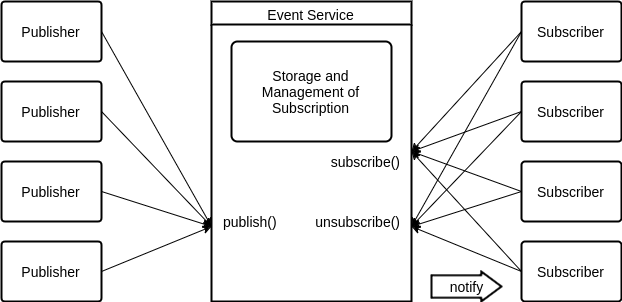
\includegraphics[width=11cm]{Resources/Images/pub-sub-general}
	\captionsetup{format=hang}
	\caption{Arsitektur dasar pada Pub/Sub \citep{eugster_many_2003}}
	\label{fig:pub-sub-general}
\end{figure}


Paradigma \textit{publish/subscribe} memiliki sifat \textit{loose coupling}. Pemisahan (\textit{decoupling}) informasi yang terjadi antara \textit{subscriber} dan \textit{publisher} dapat dibedakan ke dalam 3 (tiga) dimensi, sebagaimana diilustrasikan pada Gambar \ref{fig:space-time-sync-decoupling}. \textit{Decoupling} informasi tersebut berlangsung sebagai berikut:

\begin{enumerate}
\item \textit{Space decoupling.} \\
Interaksi antara \textit{publisher} dan \textit{subscriber} tidak perlu saling mengetahui satu dengan yang lain. \textit{Publisher} mengirimkan \textit{event}, dan \textit{subscriber} menerima \textit{event} secara tidak langsung melalui \textit{event service}. \textit{Publisher} biasanya tidak memiliki referensi tentang \textit{subscriber}. Begitu juga sebaliknya, \textit{subscriber} biasanya tidak memegang referensi tentang \textit{publisher}.
\item \textit{Time decoupling.} \\
Pihak-pihak yang berinteraksi tidak harus berinteraksi pada waktu yang bersamaan. \textit{Publisher} dapat mengirimkan \textit{event} pada saat \textit{subscriber} dalam kondisi terputus (\textit{offline}). Begitu juga sebaliknya, \textit{subscriber} tetap dapat menerima \textit{event}, meskipun \textit{original publisher} sedang dalam kondisi terputus (\textit{offline}).
\item \textit{Synchronizing decoupling.} \\
\textit{Publisher} dan \textit{subscriber} tidak berada dalam \textit{main flow}, sehingga tidak berinteraksi secara \textit{synchronous}. \textit{Publisher} tetap dapat mengirimkan informasi meskipun sedang memproduksi \textit{event} lain dan \textit{subscriber} tetap dapat memperoleh informasi meskipun sedang mengerjakan tugas yang lain. 
\end{enumerate}


\begin{figure}[!]
	\centering
	\begin{subfigure}[t]{9cm}
		\centering
		
\includegraphics[width=\textwidth]{Resources/Images/space-decoupling}
		\caption{\textit{Space Decoupling}}
		\label{fig:space-decoupling}
	\end{subfigure}%
	
	\begin{subfigure}[t]{10cm}
		\centering
		
\includegraphics[width=\textwidth]{Resources/Images/time-decoupling}
		\caption{\textit{Time Decoupling}}
		\label{fig:time-decoupling}
	\end{subfigure}%
	
	\begin{subfigure}[t]{9cm}
		\centering
		
\includegraphics[width=\textwidth]{Resources/Images/sync-decoupling}
		\caption{\textit{Sync Decoupling}}
		\label{fig:sync-decoupling}
	\end{subfigure}
	\captionsetup{format=hang}
	\caption{Pemisahan informasi pada Pub/Sub \citep{eugster_many_2003}}
	\label{fig:space-time-sync-decoupling}
\end{figure}

%-----------------------------------------------------------------------------%
\chapter{\babTiga}
%-----------------------------------------------------------------------------%
%\todo{tambahkan kata-kata pengantar bab 1 disini}


Metodologi penelitian yang akan dilakukan di dalam penelitian ini adalah \textit{Design Science Research Methods and Patterns} \citep{vaishnavi_design_2007}. Metodologi penelitian terdiri dari 5 (lima) tahapan seperti digambarkan pada Gambar \ref{fig:design-science-research-methodology} yaitu: \textit{Awareness of Problem}, \textit{Suggestion}, \textit{Development}, \textit{Evaluation}, dan \textit{Conclusion}.


\begin{figure}[h]
	\centering
	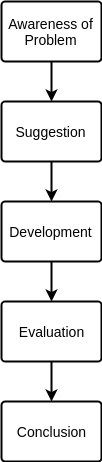
\includegraphics[width=3cm]{Resources/Images/design-science-research-methodology}
	\caption{Tahapan \textit{Design Science Research Methods and Patterns}}
	\label{fig:design-science-research-methodology}
\end{figure}


%-----------------------------------------------------------------------------%
\section{\textit{Awareness of Problem}}
%-----------------------------------------------------------------------------%
Langkah pertama dalam \textit{Design Science Research Methods and Patterns} adalah \textit{awareness of problem}. Langkah ini merupakan proses identifikasi dan definisi masalah. Permasalahan yang diidentifikasi dapat tersusun dari permasalahan nyata (\textit{real problem}) maupun permasalahan penelitian (\textit{research problem}). \textit{Real problem} diidentifikasi melalui analisis dan wawancara dengan \textit{subject matter}. Sementara \textit{research problem} diidentifikasi dari riset-riset yang meneliti permasalahan yang terkait dengan \textit{real problem}.


%-----------------------------------------------------------------------------%
\section{\textit{Suggestion}}
%-----------------------------------------------------------------------------%
Setelah masalah terdefinisikan, maka tahapan berikutnya adalah menemukan solusi dari masalah tersebut. Serangkaian analisis dan \textit{preliminary research} dilakukan untuk menemukan kandidat solusi dari permasalahan. Pada tahapan ini, akan diperoleh keluaran berupa \textit{tentative design} atau \textit{design overview}.


%-----------------------------------------------------------------------------%
\section{\textit{Development}}
%-----------------------------------------------------------------------------%
\textit{Tentative design} yang diperoleh pada tahap sebelumnya kemudian dikembangkan dan diimplementasikan pada tahap ini. Elaborasi dari \textit{tentative design} memerlukan kreatifitas. Complete design diimplementasikan dalam sejumlah bahasa pemrograman yang bervariasi, kemudian dikombinasikan dengan sejumlah software untuk membentuk sebuah prototype sistem. Sebuah mekanisme komunikasi juga dipilih pada tahap ini untuk mendukung implementasi dari sistem.


%-----------------------------------------------------------------------------%
\section{\textit{Evaluation}}
%-----------------------------------------------------------------------------%
Prototype sistem yang diimplementasikan pada tahap sebelumnya kemudian diuji dengan menggunakan serangkaian skenario. Sejumlah data juga digunakan pada tahapan ini. Hasil pengujian kemudian direpresentasikan dalam tabel dan grafik untuk memudahkan dalam menarik kesimpulan.


%-----------------------------------------------------------------------------%
\section{\textit{Conclusion}}
%-----------------------------------------------------------------------------%
Kesimpulan merupakan tahapan akhir dari penelitian. Kesimpulan yang diambil merupakan harus dapat menjawab masalah yang didefinisikan.






%-----------------------------------------------------------------------------%
\chapter{\babEmpat}
%-----------------------------------------------------------------------------%


Bab ini menjelaskan tentang perancangan sistem usulan, yaitu sistem rekomendasi lokasi pencacahan. Sebelum dijelaskan tentang sistem usulan, terlebih dahulu akan dilakukan eksperimen dan analisis terhadap solusi yang telah ada.


%-----------------------------------------------------------------------------%
\section{Analisis}
\label{sec:analysis}
%-----------------------------------------------------------------------------%
Pada kondisi saat ini (sistem berjalan), lokasi pencacahan sudah ditentukan sejak awal dengan menggunakan metode sampling tertentu. Pada tahap perancangan, sejumlah petugas direkrut dan ditugas pada sejumlah lokasi pencacahan. Pengalokasian seringkali dilakukan secara subjektif berdasarkan kedekatan lokasi pencacahan dengan domisili petugas pencacahan. Akibatnya, terjadi ketidakmerataan beban kerja dan variasi total waktu penyelesaian pekerjaan yang sangat tinggi antar petugas. 

Untuk mengatasi masalah ini, algoritma MDVRP dipilih karena memiliki karakteristik yang serupa dengan permasalahan alokasi petugas, yakni: 

\begin{enumerate}
	\item Terdapat lebih dari satu kendaraan. Tiap-tiap kendaraan memiliki depot yang berbeda. Hal ini analog dengan permasalahan alokasi petugas yang melibatkan lebih dari satu pencacah dan tiap-tiap pencacah memiliki titik mulai pencacahan yang berbeda. 
	\item Terdapat biaya yang harus dikeluarkan untuk melakukan perjalanan dari satu pelanggan ke pelanggan yang lain. Ini sejalan dengan konsep dalam pencacahan, yaitu terdapat biaya untuk mengunjungi satu responden ke responden lainnya. 
\end{enumerate}

Pada proses pencacahan, biaya dapat berupa waktu tempuh, jarak tempuh, atau biaya perjalanan. Dalam penelitian ini, waktu tempuh dipilih sebagai representasi dari biaya karena waktu tempuh menggambarkan tingkat kesulitan akses dalam mengunjungi tiap-tiap wilayah kerja. Semakin sulit akses ke suatu wilayah, semakin lama waktu tempuh yang diperlukan. 

Eksperimen dilakukan untuk membuktikan fisibilitas algoritma MDVRP dalam penyelesaian permasalahan alokasi petugas. Eksperimen melibatkan 2 (dua) komponen utama:
\begin{enumerate}
	\item Sejumlah pencacah dengan depotnya masing-masing. 
	\item Sejumlah lokasi pencacahan/blok sensus yang setiap blok sensusnya memiliki beberapa responden. 
\end{enumerate}

\autoref{ssec:mtsp_dataset} hingga \autoref{ssec:hasil-analisis} menyajikan penjelasan rinci mengenai langkah-langkah yang dilakukan dalam eksperimen. 

%-----------------------------------------------------------------------------%
\subsection{Dataset}
\label{ssec:mtsp_dataset}
%-----------------------------------------------------------------------------%
\subsubsection{Lokasi Pencacahan}
%-----------------------------------------------------------------------------%
Merujuk kepada konsep MDVRP, lokasi pencacahan dapat dianalogikan sebagai pelanggan yang akan dikunjungi oleh petugas pencacahan (kendaraan). Pengujian dilakukan dengan menggunakan data 182 lokasi nagari/kelurahan yang bersumber dari data wilayah administratif di Kabupaten Pesisir Selatan, Provinsi Sumatera Barat. Masing-masing lokasi memiliki atribut ID dan posisi koordinat menurut garis lintang dan bujur, seperti yang terlihat pada \autoref{tbl:enumeration_locations}.


\begin{table*}[!]
	\centering
	\ra{1.3}
	\captionsetup{format=hang}
	\caption{Lokasi Pencacahan}
	\label{tbl:enumeration_locations}
	\begin{tabular}{lcc}
		\toprule
		& \multicolumn{2}{c}{Koordinat}\\
		\cmidrule{2-3}
		& Lintang & Bujur\\ 
		\midrule
		1302011001 & -2.3504 & 101.1434\\ 
		1302011002 & -2.4233 & 101.0285\\ 
		1302011003 & -2.3798 & 101.0427\\ 
		1302011004 & -2.3884 & 101.049\\ 
		1302011005 & -2.3936 & 101.0546\\
		...\\
		1302110019 & -1.2387 & 100.4853\\ 
		1302110020 & -1.1408 & 100.4938\\ 
		1302110021 & -1.0883 & 100.4652\\ 
		1302110022 & -1.0886 & 100.489\\ 
		1302110023 & -1.1523 & 100.4978\\
		\bottomrule
	\end{tabular}
\end{table*}


%-----------------------------------------------------------------------------%
\subsubsection{Petugas Pencacahan}
%-----------------------------------------------------------------------------%
Berdasarkan konsep MDVRP, petugas pencacahan diibaratkan sebagai kendaraan yang harus berpindah dari satu lokasi ke lokasi lain secara berurutan. Selain memiliki atribut ID, masing-masing pencacah juga dilengkapi dengan atribut depot, yaitu lokasi di mana pencacah harus memulai dan mengakhiri kunjungan. Eksperimen ini menggunakan 15 pencacah dengan lokasi depot yang bervariasi, seperti contoh yang tercantum pada \autoref{tbl:enumerator}.


\begin{table*}[!]
	\centering
	\ra{1.3}
	\captionsetup{format=hang}
	\caption{Pencacah}
	\label{tbl:enumerator}
	\begin{tabular}{lcc}
		\toprule
		& \multicolumn{2}{c}{Koordinat Depot}\\
		\cmidrule{2-3}
		& Lintang & Bujur\\ 
		\midrule
		1302011008 & -2.3905 & 101.1214\\
		1302012003 & -2.199 & 101.1188\\
		1302020006 & -2.1225 & 101.0687\\
		...\\
		1302100002 & -1.23265 & 100.54314\\
		1302101005 & -1.19831 & 100.58078\\
		1302110003 & -1.2475 & 100.4745\\
		\bottomrule
	\end{tabular}
\end{table*}


%-----------------------------------------------------------------------------%
\subsubsection{Jarak dan Waktu Tempuh}
\label{ss:distance-duration-matrix}
%-----------------------------------------------------------------------------%
Jarak dan waktu tempuh antar lokasi pencacahan digunakan sebagai penimbang dalam penentuan rekomendasi lokasi. Penghitungan jarak dan waktu tempuh dapat dilakukan dengan cara manual (menggunakan hasil survei lokasi dan perkiraan \textit{subject matter}) atau memanfaatkan \textit{Google Directions API} \citep{google_google_2016}. 


Secara teknis, \textit{Google Direction API} lebih unggul dibandingkan metode manual karena secara otomatis memperhitungkan faktor rute tercepat, kondisi geografis, moda transportasi yang digunakan, dan kemacetan lalu lintas dalam memperkirakan jarak dan waktu tempuh. Namun, \textit{Google Direction API} mengandalkan kontribusi para pengguna \textit{Google} sebagai sumber informasi, sehingga ada kemungkinan rute-rute yang jarang dilewati akan memiliki informasi yang minim dan cenderung bias. Sebagai konsekuesinya, terdapat resiko hasil kalkukasi yang kurang tepat untuk rute-rute tersebut. 


Kode \ref{lst:google_direction_api_request} menggambarkan contoh \textit{requests URL} yang dikirimkan ke \textit{Google Direction API}. \textit{Request URL} ini dapat dieksekusi dengan menggunakan \textit{HTTP client}, seperti \textit{curl} dan \textit{wget}, atau \textit{HTTP client library}, seperti \textit{requests} dan \textit{urllib} di Python. Contoh \textit{response} Google Direction API dapat dilihat pada \autoref{fig:google_direction_api_response}.


Hasil kalkulasi jarak dan waktu tempuh kemudian disimpan dalam bentuk matriks seperti yang terlihat pada Tabel \ref{tbl:distance_duration_matrix}. Jika lokasi depot dari pencacah tidak tercakup dalam lokasi pencacahan yang ada, maka lokasi depot tersebut harus ditambahkan ke dalam matriks jarak dan waktu tempuh.


\begin{listing}[!]
	\captionsetup{format=hang}
	\caption{\textit{Google Direction API Request}}
	\label{lst:google_direction_api_request}
	\begin{minted}[showspaces=false, breaklines=true]{http}
https://maps.googleapis.com/maps/api/directions/json?origin=origin_lat,
origin_lon&destination=dest_lat,dest_lon&departure_time=timestamp&
traffic_model=best_guess&key=API_KEY
	\end{minted}
\end{listing}


\begin{figure}[!]
	\centering
	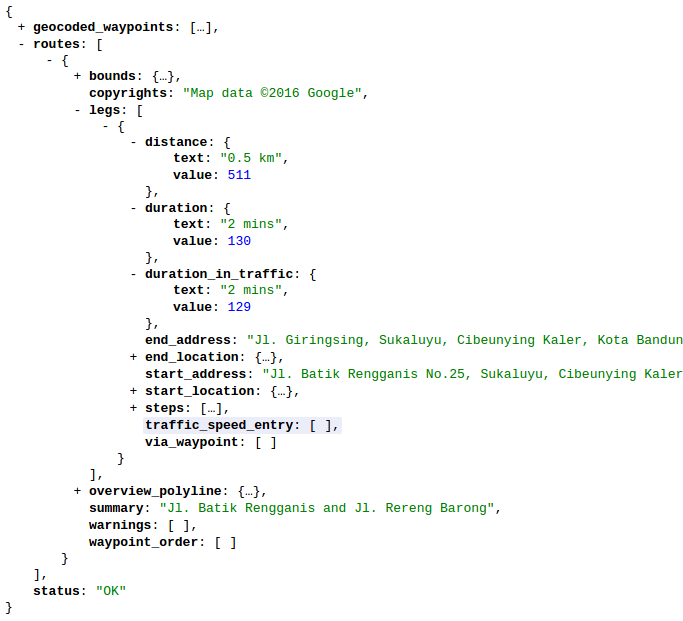
\includegraphics[width=\textwidth]{Resources/Images/google_direction_api_response}
	\captionsetup{format=hang}
	\caption{\textit{Google Direction API Response}}
	\label{fig:google_direction_api_response}
\end{figure}


\begin{table}[!]
	\centering
	\ra{1.3}
	\captionsetup{format=hang}
	\caption{Data Jarak dan Waktu Tempuh}
	\label{tbl:distance_duration_matrix}
	\begin{tabular}{llcc}
		\toprule
		Lokasi A & Lokasi B & Jarak (m) & Waktu Tempuh (det)\\
		\midrule
		1302021001 & 1302021003 & 11119 & 1055\\
		1302021001 & 1302021002 & 9373 & 868\\
		1302021001 & 1302021005 & 490 & 38\\
		1302021001 & 1302021004 & 22760 & 2044\\
		...\\
		1302040015 & 1302012010 & 77889 & 8305\\
		1302040014 & 1302100015 & 103893 & 9984\\
		1302040014 & 1302012010 & 73561 & 7546\\
		1302100015 & 1302012010 & 171636 & 16801\\
		\bottomrule
	\end{tabular}
\end{table}


%-----------------------------------------------------------------------------%
\subsection{Algoritma dan Implementasi}
\label{ssec:alg-impl}
%-----------------------------------------------------------------------------%
Terdapat banyak \textit{library} yang dapat digunakan untuk mengatasi permasalahan MDVRP, baik yang berbayar maupun \textit{open source}. Dua \textit{open source library} yang cukup banyak digunakan untuk menyelesaikan permasalahan MDVRP adalah Jsprit \citep{jsprit_jsprit_2014} dan Optaplanner \citep{optaplanner_constraint_2016}. Eksperimen ini menggunakan JSprit karena JSprit lebih berfokus pada pencarian rute serta lebih mudah untuk diimplementasikan. 


Jsprit merupakan sebuah library berbasis java yang digunakan untuk menyelesaikan permasalahan \textit{traveling salesman problem} (TSP) dan \textit{vehicle routing problems} (VRP). JSprit mencakup berbagai skenario seperti: \textit{pickups and deliveries}, \textit{back hauls}, \textit{heterogeneous fleets}, \textit{finite and infinite fleets}, \textit{multiple depots}, \textit{time windows}, \textit{open routes}, \textit{different start and end locations}, \textit{multiple capacity dimensions}, \textit{initial loads}, dan \textit{skills}. JSpirit bekerja secara terstruktur, mulai dari pendefinisan masalah, pemilihan algoritma, pencarian solusi, hingga pemilihan solusi terbaik.


%-----------------------------------------------------------------------------%
\subsubsection{Definisi Masalah}
%-----------------------------------------------------------------------------%
Pendefinisian masalah dengan \textit{library} Jsprit dilakukan dengan mendefinisikan lokasi pencacahan, para pencacah, dan matriks jarak dan waktu tempuh yang diimplementasikan dalam Kode \ref{lst:jsprit_define_locations}, Kode \ref{lst:jsprit_define_enumerators}, dan Kode \ref{lst:jsprit_define_route_weights}. Ketiga variabel ini kemudian di-\textit{build} menjadi satu dengan menggunakan \textit{syntax} yang tercantum pada Kode \ref{lst:jsprit_build_problem}.


\begin{listing}[!]
	\captionsetup{format=hang}
	\caption{Definisi Lokasi Pencacahan}
	\label{lst:jsprit_define_locations}
	\begin{minted}[showspaces=false,breaklines=true]{java}
Service.Builder builder = Service.Builder.newInstance(line[0]);

try {
	Location loc = Location.Builder.newInstance()
		.setId(line[0])
		.setCoordinate(
	Coordinate.newInstance(Double.parseDouble(line[2]), 
	Double.parseDouble(line[1]))).build();
	builder.setLocation(loc);
} catch (Exception e) {}

Service node = builder.build();
vrpBuilder.addJob(node);
	\end{minted}
\end{listing}


\begin{listing}[!]
	\captionsetup{format=hang}
	\caption{Definisi Pencacah dari File .csv}
	\label{lst:jsprit_define_enumerators}
	\begin{minted}[showspaces=false,breaklines=true]{java}
VehicleTypeImpl.Builder vehicleTypeBuilder = VehicleTypeImpl.Builder.newInstance("enumerator");
vehicleTypeBuilder.setCostPerDistance(0);
vehicleTypeBuilder.setCostPerTransportTime(1);
vehicleTypeBuilder.setCostPerServiceTime(1);
VehicleType vehicleType = vehicleTypeBuilder.build();

VehicleImpl.Builder builder = VehicleImpl.Builder.newInstance(line[0]);

try {
	Location loc = Location.Builder.newInstance()
		.setId(line[0])
		.setCoordinate(Coordinate.newInstance(
			Double.parseDouble(line[2]), Double.parseDouble(line[1])))
		.build();
	builder.setStartLocation(loc);
} catch (Exception e) {}


builder.setType(vehicleType);
VehicleImpl vehicle = builder.build();
vrpBuilder.addVehicle(vehicle);
	\end{minted}
\end{listing}


\begin{listing}[!]
	\captionsetup{format=hang}
	\caption{Definisi Penimbang Jarak dan Waktu Tempuh dari File .csv}
	\label{lst:jsprit_define_route_weights}
	\begin{minted}[showspaces=false,breaklines=true]{java}
VehicleRoutingTransportCostsMatrix.Builder costMatrixBuilder = VehicleRoutingTransportCostsMatrix.Builder.newInstance(true);

while ((line = reader.readNext()) != null) {
	try {
		costMatrixBuilder.addTransportDistance(line[0], line[1], Double.parseDouble(line[2]));
		costMatrixBuilder.addTransportTime(line[0], line[1], Double.parseDouble(line[3]));
	} catch (Exception e) {
		costMatrixBuilder.addTransportDistance(line[0], line[1], 0.0);
		costMatrixBuilder.addTransportTime(line[0], line[1], 0.0);
	}
}

VehicleRoutingTransportCosts costMatrix = costMatrixBuilder.build();
vrpBuilder.setRoutingCost(costMatrix);
	\end{minted}
\end{listing}


\begin{listing}[!]
	\captionsetup{format=hang}
	\caption{Pendefinisian Masalah}
	\label{lst:jsprit_build_problem}
	\begin{minted}[showspaces=false,breaklines=true]{java}
VehicleRoutingProblem.Builder vrpBuilder = VehicleRoutingProblem.Builder.newInstance();
vrpBuilder.setFleetSize(VehicleRoutingProblem.FleetSize.FINITE);
VehicleRoutingProblem problem = vrpBuilder.build();
	\end{minted}
\end{listing}


%-----------------------------------------------------------------------------%
\subsubsection{Konfigurasi Algoritma}
%-----------------------------------------------------------------------------%
Berdasarkan masalah yang telah didefinisikan sebelumnya, JSprit kemudian akan membuat konfigurasi algoritma. Secara \textit{default} algoritma yang digunakan adalah \textit{Tabu Search}. Selain itu, jumlah iterasi dan \textit{thread} yang digunakan juga dapat didefinisikan. Kode \ref{lst:jsprit_create_algorithm} merupakan \textit{syntax} konfigurasi algoritma yang digunakan. 


\begin{listing}[!]
	\captionsetup{format=hang}
	\caption{Penentuan Algoritma}
	\label{lst:jsprit_create_algorithm}
	\begin{minted}[showspaces=false,breaklines=true]{java}
	VehicleRoutingAlgorithm algorithm = Jsprit.Builder.newInstance(problem)
	.setProperty(Jsprit.Parameter.THREADS, 5).buildAlgorithm();
	algorithm.setMaxIterations(iterations);
	\end{minted}
\end{listing}


%-----------------------------------------------------------------------------%
\subsubsection{Pencarian Solusi dan Penentuan Solusi Terbaik}
%-----------------------------------------------------------------------------%
Pencarian solusi dilakukan dengan menggunakan algoritma yang didefinisikan pada tahap sebelumnya. Jika algoritma memproduksi lebih dari satu solusi, maka Jspirit akan melakukan pemilihan solusi terbaik seperti yang terlihat pada Kode \ref{lst:jsprit_search_solution}. Secara \textit{default}, solusi terbaik merupakan solusi yang memiliki total biaya terrendah.


\begin{listing}[!]
	\captionsetup{format=hang}
	\caption{Pencarian Solusi}
	\label{lst:jsprit_search_solution}
	\begin{minted}[showspaces=false,breaklines=true]{java}
	Collection<VehicleRoutingProblemSolution> solutions = algorithm.searchSolutions();
	VehicleRoutingProblemSolution bestSolution = Solutions.bestOf(solutions);
	\end{minted}
\end{listing}


%-----------------------------------------------------------------------------%
\subsection{Hasil dan Analisis}
\label{ssec:hasil-analisis}
%-----------------------------------------------------------------------------%
Berdasarkan hasil dari eksperimen, diperoleh rute seperti yang digambarkan pada Gambar \ref{fig:analysis_mtsp_recommendation} dan Listing \ref{lst:analysis_mtsp_recommendation} untuk detail dari setiap pencacah. Berdasarkan rute tersebut kemudian dilakukan simulasi pencacahan dengan menyertakan waktu tempuh dan lama pencacahan pada tiap-tiap lokasi. Lama pencacahan untuk tiap-tiap lokasi pencacahan dibuat dengan mengikuti distribusi normal. Pengujian dengan menggunakan 182 lokasi pencacahan dan 15 petugas pencacahan menghasilkan rata-rata dan standar deviasi waktu penyelesaian tugas sebesar:  
$$ \mu = 82,24 jam $$
$$ \sigma = 88,95 jam $$


\begin{figure}[!]
	\centering
	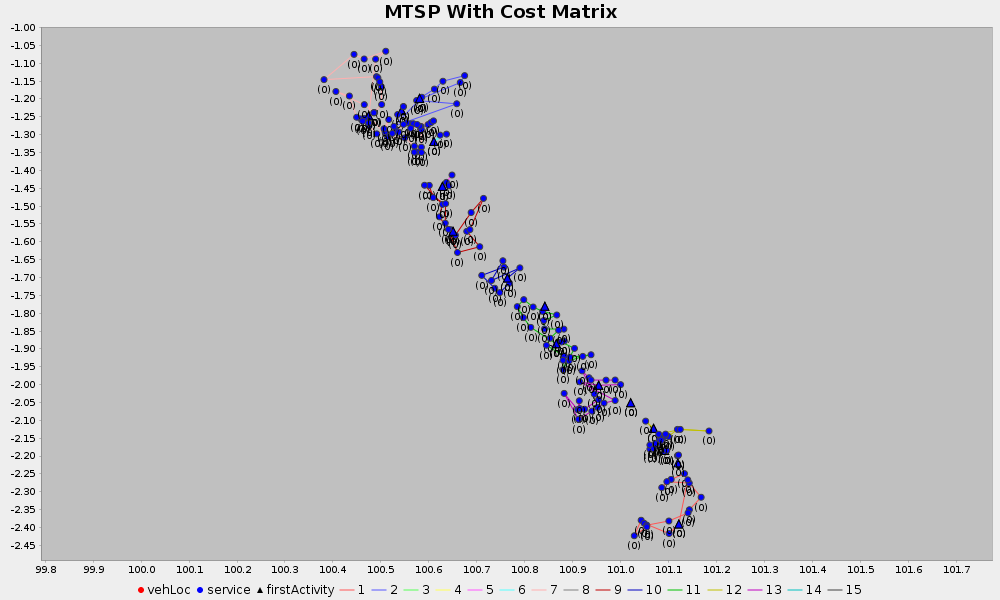
\includegraphics[width=\textwidth]{Resources/Images/analysis_mtsp_no_time_windows}
	\captionsetup{format=hang}
	\caption{Rute yang dihasilkan oleh JSprit}
	\label{fig:analysis_mtsp_recommendation}
\end{figure}


\begin{listing}[!]
	\captionsetup{format=hang}
	\caption{Detail rute yang dihasilkan oleh JSprit}
	\label{lst:analysis_mtsp_recommendation}
	\begin{minted}[showspaces=false,breaklines=true, escapeinside=||]{text}
|\textbf{1302021005}| : 1302021001 --> 1302021005
|\textbf{1302101005}| : 1302101005 --> 1302101001 --> 1302100010 --> 1302100014 --> 1302100011 --> 1302101004 --> 1302101006 --> 1302101003 --> 1302101002
|\textbf{1302070006}| : 1302070006 --> 1302070002 --> 1302070003 --> 1302080009 --> 1302080004 --> 1302080001 --> 1302080005 --> 1302080003 --> 1302070012 --> 1302070011 --> 1302070001 --> 1302070004 --> 1302070007 --> 1302070008 --> 1302070010 --> 1302070009 --> 1302070005
|\textbf{1302050007}| : 1302050007
|\textbf{1302100002}| : 1302100002 --> 1302100003 --> 1302100013 --> 1302100012
|\textbf{1302030005}| : 1302030005
|\textbf{1302110003}| : 1302110003 --> 1302100001 --> 1302090006 --> 1302090012 --> 1302090003 --> 1302090014 --> 1302090009 --> 1302090015 --> 1302090018 --> 1302090016 --> 1302090017 --> 1302090013 --> 1302090005 --> 1302090007 --> 1302090002 --> 1302090008 --> 1302090001 --> 1302100015 --> 1302100004 --> 1302100016 --> 1302090011 --> 1302090010 --> 1302100017 --> 1302100006 --> 1302100007 --> 1302100009 --> 1302100008 --> 1302100005 --> 1302110001 --> 1302110010 --> 1302110013 --> 1302110002 --> 1302110014 --> 1302110015 --> 1302110011 --> 1302110016 --> 1302110017 --> 1302110004 --> 1302110018 --> 1302110019 --> 1302110005 --> 1302110012 --> 1302110023 --> 1302110020 --> 1302110006 --> 1302110007 --> 1302110008 --> 1302110021 --> 1302110009 --> 1302110022
|\textbf{1302012003}| : 1302012007 --> 1302012003 --> 1302012008
|\textbf{1302080006}| : 1302080006 --> 1302080008 --> 1302080002 --> 1302080007
|\textbf{1302031005}| : 1302031005 --> 1302031008 --> 1302030014 --> 1302030006 --> 1302030009 --> 1302030004 --> 1302030010 --> 1302031003 --> 1302030002 --> 1302031004 --> 1302030003 --> 1302030012 --> 1302031001 --> 1302031006 --> 1302040011 --> 1302031009 --> 1302031010 --> 1302031002 --> 1302031007 --> 1302030001
|\textbf{1302060005}| : 1302060005 --> 1302060009 --> 1302060006 --> 1302060008 --> 1302060002 --> 1302060007 --> 1302060001 --> 1302060003 --> 1302060004
|\textbf{1302020006}| : 1302020006 --> 1302020015 --> 1302020011 --> 1302020009 --> 1302020010 --> 1302020001 --> 1302020003 --> 1302020005 --> 1302021006 --> 1302021002 --> 1302021007 --> 1302021008 --> 1302021003 --> 1302021009 --> 1302021004 --> 1302021010 --> 1302020016 --> 1302020017
|\textbf{1302011008}| : 1302011008 --> 1302011007 --> 1302011004 --> 1302011003 --> 1302011002 --> 1302011006 --> 1302011005 --> 1302011009 --> 1302011010 --> 1302011001 --> 1302012005 --> 1302012002 --> 1302012009 --> 1302012010 --> 1302012004 --> 1302012001 --> 1302012006
|\textbf{1302040002}| : 1302040002 --> 1302040003 --> 1302040004 --> 1302040015 --> 1302040008 --> 1302040009 --> 1302040010 --> 1302040014 --> 1302040012 --> 1302040013 --> 1302040001 --> 1302040016 --> 1302040007 --> 1302040006 --> 1302040005 --> 1302050001 --> 1302050004 --> 1302050006 --> 1302050002 --> 1302050008 --> 1302050010 --> 1302050009 --> 1302050005 --> 1302050003
|\textbf{1302090004}| : 1302090004 --> 1302090019 --> 1302090020
	\end{minted}
\end{listing}


\begin{table}[!]
	\centering
	\ra{1.3}
	\captionsetup{format=hang}
	\caption{Waktu total dari setiap rute yang dihasilkan oleh JSprit}
	\label{tbl:enumerators_total_time}
	\begin{tabular}{lc}
		\toprule
		Pencacah & Total Waktu (jam)\\
		\midrule
		1302021005 & 13.3\\
		1302101005 & 60.8\\
		1302070006 & 116\\
		1302050007 & 6\\
		1302100002 & 26.6\\
		1302030005 & 6\\
		1302110003 & 341\\
		1302012003 & 19.9\\
		1302080006 & 27.1\\
		1302031005 & 136\\
		1302060005 & 61.3\\
		1302020006 & 121\\
		1302011008 & 116\\
		1302040002 & 162\\
		1302090004 & 20.2\\
		\bottomrule
	\end{tabular}
\end{table}


Nilai standar deviasi yang tinggi menunjukkan terjadinya ketidakmerataan beban kerja antar pencacah. Ini sekaligus menunjukkan bahwa algoritma MDVRP murni kurang ideal untuk digunakan dalam penentuan rekomendasi. Hal ini terjadi karena algoritma MDVRP memproduksi solusi berupa \textit{precalculated routes} (rute yang harus dikunjungi dari awal hingga akhir tugas pencacahan) tanpa memperhitungkan faktor lamanya waktu kunjungan pada satu lokasi pencacahan. Variabel lama waktu pencacahan hanya akan tersedia jika suatu lokasi sudah selesai dikunjungi sehingga tidak bisa diikutsertakan dalam kalkulasi rekomendasi. \autoref{fig:illustration-timeline-mdvrp-no-service-time} menunjukkan ilustrasi ketidaksesuaian penggunaan algoritma MDVRP murni pada permasalahan alokasi petugas pencacahan yang dapat dijabarkan sebagai berikut:
\begin{enumerate}
	\item Terdapat 10 lokasi pencacahan yang harus dikunjungi. Algoritma MDVRP menciptakan solusi berupa \textit{precalculated routes} untuk petugas A dan B. Tiap-tiap petugas mendapatkan jumlah beban tugas yang sama besar, yakni 5 lokasi. Pada tahap ini, petugas A dan B sama-sama sudah mengetahui urutan lokasi yang akan mereka kunjungi dari awal hingga akhir kegiatan pencacahan. 
	\item Petugas pencacahan A dan B sama-sama memulai tugas pada waktu $t_{s}$ (\textit{time start}) yang digambarkan sebagai segmen berwarna hijau.
	\item Petugas A dan B mengunjungi lokasi pencacahan masing-masing (lokasi \textit{i}) yang memakan waktu selama $t_{i}$ (segmen berwarna putih). Perlu diingat bahwa lokasi $i$ yang dituju oleh petugas A berbeda dengan lokasi $i$ yang dituju oleh petugas B.
	\item Pada setiap lokasi $i$, baik petugas A maupun petugas B memerlukan waktu sebesar $t_{i.1}$ untuk menyelesaikan tugas pencacahan (segmen berwarna biru).  
	\item Petugas A dan B menyelesaikan tugas pada waktu $t_{f}$ (\textit{time finish}) yang digambarkan sebagai segmen berwarna merah muda. 
\end{enumerate}

Dari \autoref{fig:illustration-timeline-mdvrp-no-service-time}, terlihat bahwa kalkulasi rekomendasi rute tanpa melibatkan lama pencacahan mengakibatkan $t_{i}$ dan $t_{i.1}$ yang tidak setara antara petugas A dan B. Hal ini terlihat dari posisi $t_{f}$ petugas A yang jauh berbeda dengan posisi $t_{f}$ petugas B pada \textit{timeline} masing-masing. Petugas A mendapatkan rute dengan rata-rata \textit{service time} ($t_{i.1}$) yang lebih panjang sehingga $t_{f}$ petugas A menjadi lebih besar dibandingkan $t_{f}$ petugas B. Perbedaan yang paling signifikan terlihat pada lokasi pencacahan kedua ($i = 2$), ketika petugas A memiliki $t_{2.1}$ yang hampir 3 (tiga) kali lebih besar dari $t_{2.1}$ petugas B. Sebagai dampaknya, terjadi ketimpangan dalam total waktu penyelesaian pencacahan antar petugas. Beban tugas petugas A menjadi jauh lebih berat dibandingkan petugas B. 

\begin{figure}[!]
	\centering
	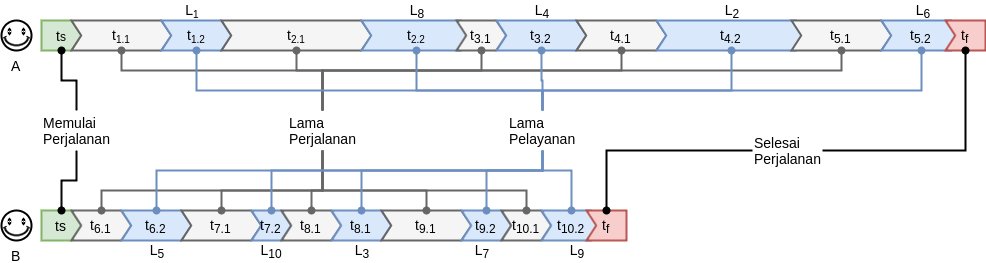
\includegraphics[width=\textwidth]{Resources/Images/illustration-timeline-mdvrp}
	\caption{Ilustrasi \textit{Timeline} Rute yang Dikalkulasi Tanpa Melibatkan Waktu Pencacahan}
	\label{fig:illustration-timeline-mdvrp-no-service-time}
\end{figure}


Untuk mengatasi masalah ini diperlukan suatu mekanisme kalkulasi rekomendasi yang tidak terikat pada lama waktu pencacahan. Mekanisme ini kemudian akan dikombinasikan dengan algoritma MDVRP sehingga menghasilkan suatu metode baru yang dapat menutupi kelemahan MDVRP sekaligus memberikan rekomendasi rute yang lebih adil kepada semua petugas pencacahan. 


%-----------------------------------------------------------------------------%
\section{Perancangan Solusi}
\label{sec:design}
%-----------------------------------------------------------------------------%
Hasil eksperimen pada \autoref{ssec:hasil-analisis} menunjukkan bahwa mekanisme kalkulasi yang bebas dari `lama pencacahan' diperlukan untuk menghilangkan bias dan kesenjangan rute untuk tiap-tiap petugas. Solusi yang diusulkan untuk mengatasi masalah ini adalah dengan melakukan penghitungan rute secara bertahap dengan melakukan `hibridisasi' antara algoritma MDVRP dengan suatu mekanisme \textit{real time}. Idenya adalah, alih-alih menghitung rute secara lengkap diawal pencacahan, lebih baik rute dihitung secara bertahap secara \textit{real time} dengan memanfaatkan `lokasi terkini' dari petugas sebagai depot yang baru pada setiap tahapnya. Pada saat awal pencacahan, petugas hanya mengetahui lokasi pertama yang akan mereka kunjungi. Setelah menyelesaikan tugas pencacahan pada lokasi tersebut, petugas harus mengirimkan permintaan ke \textit{server} guna mengetahui lokasi pencacahan berikutnya.

\autoref{fig:illustration-timeline-realtime-mdvrp} menggambarkan penerapan \textit{real time} MDVRP untuk mengatasi permasalahan alokasi petugas pencacahan yang dijabarkan sebagai berikut:
\begin{enumerate}
	\item Terdapat 10 lokasi pencacahan yang harus dikunjungi. Petugas pencacahan A dan B sama-sama memulai tugas pada waktu $t_{s}$ (segmen berwarna hijau). Berbeda dengan mekanisme pada \autoref{fig:illustration-timeline-mdvrp-no-service-time}, pada tahap ini, petugas A dan B sama-sama tidak memiliki pengetahuan apapun tentang urutan lokasi yang harus mereka kunjungi. 
	\item Pada waktu $t_{1}$ (segmen berwarna kuning), A dan B mengirimkan permintaan ke \textit{server} untuk mendapatkan lokasi pertama yang harus mereka kunjungi. 
	\item A dan B berjalan menuju lokasi pencacahan masing-masing (lokasi \textit{i}) yang memerlukan waktu tempuh sebesar $t_{i.1}$ (segmen berwarna putih). Lokasi $i$ yang dituju oleh petugas A berbeda dengan lokasi $i$ yang dituju oleh petugas B.
	\item A dan B menyelesaikan tugas pencacahan di lokasi pertama yang menghabiskan waktu sebesar $t_{i.2}$ (segmen berwarna biru).
	\item Setelah menyelesaikan tugas di lokasi pertama, A dan B mengirimkan \textit{request} ke server untuk mengetahui lokasi berikutnya yang harus dikunjungi. Server kemudian melakukan rekalkulasi rute dengan melakukan pengecekan terhadap 8 lokasi yang belum dikunjungi dan mencocokkannya dengan `lokasi terkini' dari petugas. Lokasi pencacahan berikutnya yang merupakan lokasi terbaik jika dihitung dari `lokasi terkini', akan dikirimkan sebagai balasan terhadap permintaan yang telah dikirimkan oleh petugas. 
	\item A dan B melanjutkan tugas pencacahan ke lokasi berikutnya (lokasi $i = 2$). Setiap lokasi memerlukan waktu tempuh sebesar $t_{i.1}$ dan waktu penyelesaian pencacahan (\textit{service time}) sebesar $t_{i.2}$. Proses pada poin 2 hingga 6 akan terus berulang hingga seluruh lokasi target pencacahan selesai dikunjungi. 
	\item Petugas A dan B menyelesaikan tugas pada waktu $t_{f}$ (segmen berwarna merah muda) yang hampir sama. Dari \autoref{fig:illustration-timeline-realtime-mdvrp} terlihat bahwa jumlah lokasi yang dikunjungi oleh petugas A lebih sedikit dibandingkan petugas B. Hal ini dikarenakan petugas A memerlukan waktu yang lebih lama untuk melakukan perjalanan ke lokasi serta menyelesaikan tugas pencacahan di lokasi tersebut. 
\end{enumerate}


Mayoritas \textit{real time system} diimplementasikan dengan menggunakan \textit{Web service}. Namun, sistem kerjanya yang \textit{synchronous} (\textit{request} dan \textit{reply} harus diproses secara berurutan) menyebabkan \textit{web service} tidak cocok digunakan untuk aplikasi yang bersifat \textit{information driven} \citep{muhl_large-scale_2002}. Sebagai alternatif, mekanisme \textit{publish/subscribe} dipilih karena memungkinkan terjadinya komunikasi yang \textit{asynchronous} antara \textit{server (publisher)} dan \textit{client (subscriber)}, yaitu komunikasi yang tetap dapat berjalan walaupun salah satu pihak sedang dalam kondisi \textit{offline}.


\begin{figure}[!]
	\centering
	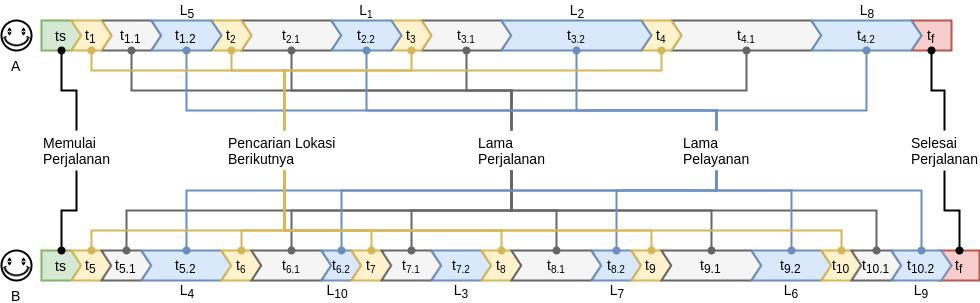
\includegraphics[width=\textwidth]{Resources/Images/illustration-timeline-realtime-mdvrp}
	\captionsetup{format=hang}
	\caption{Ilustrasi \textit{Timeline} Penerapan MDVRP Secara \textit{Real Time}}
	\label{fig:illustration-timeline-realtime-mdvrp}
\end{figure}

%-----------------------------------------------------------------------------%
\subsection{Garis Besar Sistem Usulan}
%-----------------------------------------------------------------------------%
Sistem usulan untuk rekomendasi lokasi pencacahan dirancang berdasarkan arsitektur \textit{publish/subscribe} yang terdiri dari 3 (tiga) komponen utama, yaitu: \textit{publisher} rekomendasi, petugas pencacahan yang berperan sebagai \textit{subscriber}, dan \textit{message broker} yang berperan sebagai penerus pesan (\textit{message router}). \autoref{fig:system-overview} memberikan ilustrasi komponen yang menyusun sistem rekomendasi lokasi pencacahan usulan.


\begin{figure}[!]
	\centering
	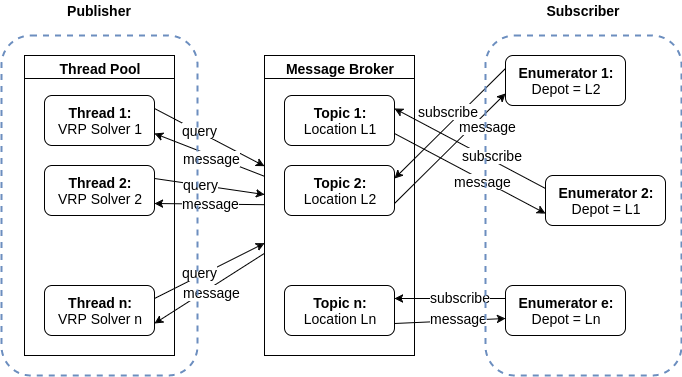
\includegraphics[width=\textwidth]{Resources/Images/system-overview}
	\captionsetup{format=hang}
	\caption{Garis Besar Sistem Usulan}
	\label{fig:system-overview}
\end{figure}


Komunikasi antara \textit{publisher} dan \textit{subscriber} terjadi atas dasar kesamaan topik (\textit{event}). Topik diperoleh dari konteks setiap pencacah yang dapat berupa jenis kelamin, tingkat pendidikan, umur, pengalaman, atau domisili/lokasi pencacah. Pada penelitian ini, `lokasi terkini' dari pencacah dipilih sebagai topik karena bersifat unik, yaitu setiap lokasi pencacahan hanya akan dikunjungi oleh satu orang pencacah saja dan tidak akan ada lebih dari satu pencacah dengan `lokasi terkini' yang sama.


%-----------------------------------------------------------------------------%
\subsection{\textit{Publisher} Rekomendasi}
\label{ssec:publisher}
%-----------------------------------------------------------------------------%
Berdasarkan konsep dasar mekanisme \textit{publish/subscribe}, \textit{publisher} akan mengirimkan informasi ke seluruh \textit{subscriber} tanpa melihat apakah \textit{subscriber} tersebut memang men-\textit{subscribe} topik dari informasi yang bersangkutan atau tidak. Akibatnya informasi yang dikirim banyak yang tidak tepat sasaran sehingga komunikasi yang berlangsung menjadi tidak efisien. Untuk mengatasi inefisiensi komunikasi ini, perlu dilakukan beberapa penyesuaian agar \textit{publisher} hanya akan mengirimkan informasi kepada \textit{subscriber} yang bersesuaian. 

Pada saat seorang petugas pencacahan yang berperan sebagai \textit{subscriber} mengirimkan permintaan `lokasi pencacahan yang harus dituju' kepada \textit{publisher}, permintaan ini tidak langsung diterima oleh \textit{publisher}, melainkan ditampung oleh \textit{message broker}. \textit{Publisher} perlu mengecek \textit{message broker} secara berkala untuk mendeteksi ada atau tidaknya \textit{request} baru dengan menggunakan \textit{thread} $TopicWatcher$ yang dideskripsikan pada \autoref{alg:topic-watcher} serta digambarkan dengan \textit{flowchart} pada \autoref{fig:topic-watcher}. 


\begin{algorithm}[!]
	\captionsetup{format=hang}
	\caption{TopicWatcher}
	\label{alg:topic-watcher}
	\begin{algorithmic}[1]
		\renewcommand{\algorithmicrequire}{\textbf{Input:}}
		\renewcommand{\algorithmicensure}{\textbf{Output:}}
		\REQUIRE $None$
		\ENSURE  $None$
		\\ $TP$ = Threadpool
		\\ $N$ = Number of locations
		\\ $M$ = Number of enumerators
		\WHILE {true}
		\STATE $C \leftarrow readAvailableTopicFromBroker()$	// channel
		\FOR {$m = 1$ to $len(C)$}
		\FOR {$n = 1$ to $N$}
		\IF {($C_m == L_n$)}
		\STATE $T_n = Thread(C_m, E_1...E_M, (unassigned) L_1...L_N)$		// E = enumerator
		\STATE submitThreadToThreadpool($T_n$, $TP$)
		\ENDIF
		\ENDFOR
		\ENDFOR
		\ENDWHILE
	\end{algorithmic}
\end{algorithm}


\begin{figure}[!]
	\centering
	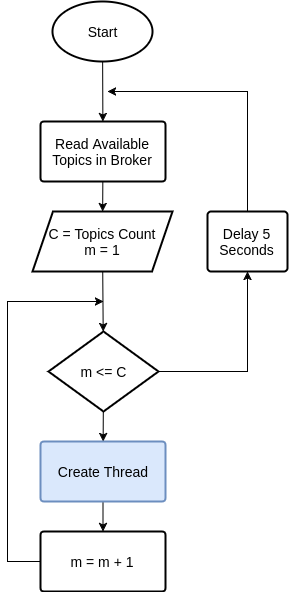
\includegraphics[width=6.3cm]{Resources/Images/topic-watcher}
	\captionsetup{format=hang}
	\caption{\textit{\textit{Flowchart} Topic Watcher}}
	\label{fig:topic-watcher}
\end{figure}


Untuk setiap permintaan yang diterima, \textit{publisher} akan menyiapkan sebuah \textit{thread} baru dengan menggunakan `lokasi terkini' dari \textit{subscriber} (petugas) sebagai ID. \textit{Thread} ini dilengkapi dengan sebuah $VRP solver procedure$ (\autoref{alg:vrp-worker}) yang akan melakukan pencarian solusi/rute. Seluruh \textit{thread} dari masing-masing topik ditampung di dalam sebuah \textit{threadpool} yang menangani \textit{thread} berdasarkan urutan waktu kedatangan. Pada akhir proses pencacahan ketika seluruh lokasi pencacahan telah dialokasikan kepada petugas, ukuran \textit{threadpool} ini akan sama dengan jumlah seluruh topik yang tersedia. 


\textit{Thread-thread} di dalam \textit{threadpool} dieksekusi satu per satu sesuai dengan waktu kedatangan. Setiap eksekusi akan melibatkan \textit{VRPSolver procedure} yang mengikutsertakan $M$ \textit{subscribers} (petugas pencacahan) dan \textit{unassigned} N lokasi pencacahan. \textit{VRPSolver procedure} harus mengikutsertakan seluruh \textit{subscriber} untuk memastikan diperolehnya solusi terbaik yang bersifat global (\textit{global best solution}). \autoref{fig:global-best-greedy-solution} memberikan ilustrasi tentang \textit{Global Best Solution} dengan penjelasan sebagai berikut:
\begin{enumerate}
	\item Petugas A dan B masing-masing melakukan pencacahan pada lokasi 5 dan 6 dan `lokasi terkini' mereka akan diperbarui.
	\item Petugas B menyelesaikan pekerjaannya lebih cepat dari petugas A dan segera mengirimkan permintaan `lokasi pencacahan berikutnya'. Sistem kemudian menghitung dan mengirimkan `lokasi berikutnya' berdasarkan `lokasi terkini' dari petugas B. 
	\item Jika kalkulasi rute hanya melibatkan 1 petugas yang bersangkutan saja, maka \textit{VRPSolver procedure} akan merekomendasikan lokasi terdekat dari `lokasi terkini' petugas B, yakni lokasi 7. Namun, solusi yang dibuat berdasarkan sudut pandang lokal (\textit{local best solution}) seperti ini, dapat `merugikan' petugas lain yang tidak ikut dalam penghitungan. 
	\item Sebagai gambaran, misalkan saat A selesai melakukan pencacahan dan mengirimkan permintaan `lokasi berikutnya', lokasi 7 sudah tidak tersedia lagi bagi A. Rekomendasi terbaik yang bisa diberikan oleh sistem adalah lokasi 1 yang memiliki jarak yang cukup jauh dari A. 
	\item Rekomendasi yang lebih tepat dapat diperoleh jika kalkulasi rute mengikutsertakan seluruh pencacah. Pelibatan terhadap `lokasi terkini' dari seluruh petugas akan menghasilkan solusi yang terbaik dari sudut pandang seluruh pencacah (\textit{global best solution}), sehingga petugas B akan mendapatkan lokasi 3 dan petugas A akan mendapatkan lokasi 7. 

\end{enumerate}

Proses pencarian solusi akan berakhir ketika sudah tidak ada lagi lokasi pencacahan yang berstatus `belum teralokasi'. Adapun \textit{VRP Solver Procedure} dijelaskan secara lebih rinci pada \autoref{ssec:vrp-solver}.


\begin{figure}[!]
	\centering
	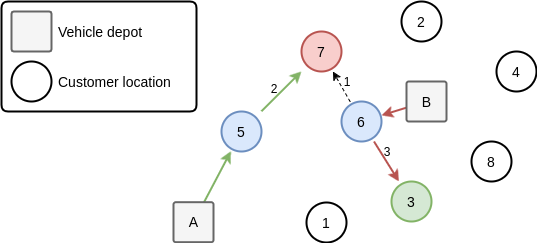
\includegraphics[width=12cm]{Resources/Images/global-best-greedy-solution}
	\captionsetup{format=hang}
	\caption{Ilustrasi \textit{Global Best Solution}}
	\label{fig:global-best-greedy-solution}
\end{figure}


\begin{algorithm}[!]
	\captionsetup{format=hang}
	\caption{\textit{RecommendationPublisher}}
	\label{alg:vrp-worker}
	\begin{algorithmic}[1]
		\renewcommand{\algorithmicrequire}{\textbf{Input:}}
		\renewcommand{\algorithmicensure}{\textbf{Output:}}
		\REQUIRE $TP$		// threadpool
		\ENSURE  $None$
		
		\WHILE {true}
		\STATE $T$ = popFirstThreadOrWaitNewThreadFromThreadpool()
		\STATE $R$ = VRPSolver($T$)
		\FOR {$j = 1$ to $len(R)$}
		\STATE $r$ = publish($C_{R_j}$, $R_j$)
		\IF {($r > 0$)}
		\STATE cancelSolver($T_j$)
		\ELSIF {($C_{T_i} \notin C_{R_j}$)}
		\STATE $T_i = Thread(C_{T_i}, V_m, (unassigned) E_1...E_N)$
		\ENDIF
		\ENDFOR
		\ENDWHILE	
	\end{algorithmic}
\end{algorithm}


Jumlah rute yang dihasilkan oleh \textit{VRPSolver} akan berkisar antara 1 (satu) hingga $M$ rute. $M$ merujuk pada jumlah seluruh petugas pencacahan yang diikutsertakan dalam kalkulasi rute. Setiap rute $R_m$ $(1 \leq m \leq M)$ yang dihasilkan oleh \textit{VRPSolver} akan dikirimkan kepada petugas $m$ yang merupakan \textit{subscriber} topik (lokasi) $C_n$ $(1 \leq n \leq N)$. \textit{Message broker} kemudian akan melaporkan status pengiriman informasi kepada \textit{publisher} (\textit{`success'} atau \textit{`failed'}). Mekanisme kerja \textit{publisher} rekomendasi diilustrasikan dengan menggunakan \textit{flowchart} pada \autoref{fig:recommendation-publisher}.


\begin{figure}[!]
	\centering
	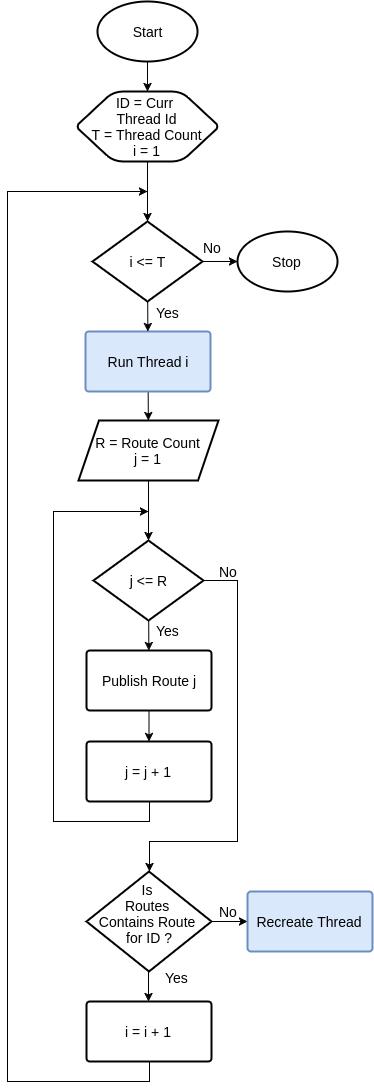
\includegraphics[width=8cm]{Resources/Images/recommendation-publisher}
	\captionsetup{format=hang}
	\caption{\textit{Flowchart recommendation publisher}}
	\label{fig:recommendation-publisher}
\end{figure}


\autoref{fig:timeline-illustration} memberikan gambaran umum tentang proses yang terjadi sejak permintaan lokasi dikirim oleh petugas hingga solusi/rute diperoleh. Petugas B mengirimkan permintaan yang diterima oleh \textit{message broker}. \textit{TopicWatcher} yang memantau \textit{message broker} mengetahui keberadaan permintaan baru ini dan kemudian melaporkannya kepada \textit{publisher}. \textit{Publisher} kemudian menciptakan sebuah \textit{thread} yang mengandung \textit{VRPSolver procedure}. Saat \textit{thread} dieksekusi, \textit{VRPSolver procedure} akan melakukan kalkulasi solusi/rute terbaik dengan mengikutsertakan seluruh $M$ petugas dan lokasi yang masih berstatus \textit{unassigned}. \textit{Thread} hanya dapat dijalankan secara berurutan berdasarkan prinsip `satu dalam satu waktu' (\textit{once at a time}). Sebagai konsekuensinya, ketika petugas A mengirimkan \textit{request} baru, \textit{thread} untuk \textit{request} A tetap akan diciptakan, namun dibiarkan dalam status \textit{idle}. \textit{Thread} A harus menunggu hingga \textit{thread} sebelumnya (\textit{thread} B) selesai diproses. 

Saat \textit{thread} B selesai diproses, \textit{thread} B tidak hanya menghasilkan rute untuk petugas B, tapi juga untuk sejumlah $m$ petugas lainnya ($1 \leq m \leq M$). Rute-rute ini akan dikirimkan kepada petugas yang bersesuaian. Jika suatu rute $R_m$ berhasil diterima oleh petugas $m$, maka \textit{thread} yang berasosiasi dengan rute tersebut akan dihentikan (\textit{terminate}). Dalam \autoref{fig:timeline-illustration}, \textit{thread} B menghasilkan solusi/rute untuk petugas A dan B dan kedua rute ini berhasil diterima dengan baik oleh masing-masing petugas. Dalam hal ini, \textit{thread} A dan \textit{B} dinilai tidak lagi dibutuhkan sehingga kedua \textit{thread} tersebut akan dihentikan. Penghentian ini dilakukan untuk mencegah terjadinya penghitungan ganda terhadap rute yang sudah diterima oleh \textit{subscriber} (petugas). 


\begin{figure}[!]
	\centering
	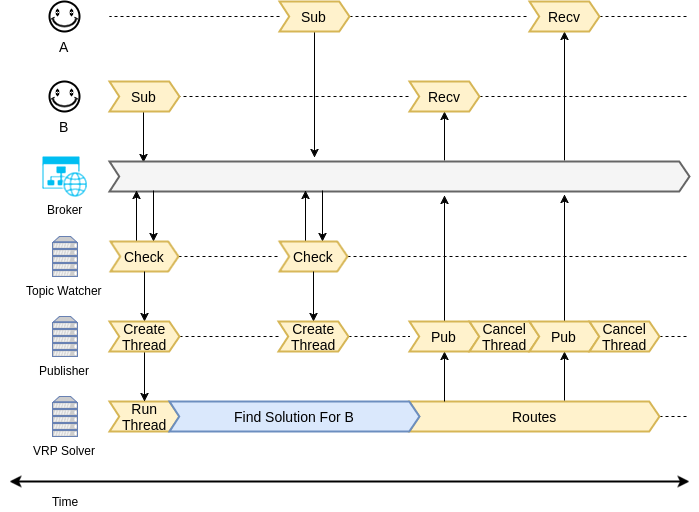
\includegraphics[width=\textwidth]{Resources/Images/timeline-illustration}
	\captionsetup{format=hang}
	\caption{Ilustrasi \textit{Timeline} Proses Pencarian Solusi Berdasarkan}
	\label{fig:timeline-illustration}
\end{figure}


Pada praktiknya, dapat terjadi suatu kondisi ketika \textit{VRPSolver procedure} gagal mendapatkan rute untuk petugas B. Pada kondisi demikian, \textit{thread} B akan diproses ulang dengan hanya melibatkan 1 (satu) petugas B saja dan sejumlah lokasi yang masih berstatus \textit{unassigned}. Ini dilakukan untuk memberikan jaminan bahwa akan selalu ada solusi/rute untuk setiap \textit{request}. 


Pada \autoref{ssec:pub-sub-mechanism} dijelaskan bahwa karakteristik \textit{loose coupling} pada mekanisme \textit{publish/subscribe} membuat \textit{publisher} dan \textit{subscriber} mampu berkomunikasi secara fleksibel, tanpa perlu mengetahui identitas masing-masing. Namun kondisi ini mengakibatkan informasi mengenai `lokasi terkini' dari \textit{subscriber} tidak dapat diperoleh. Untuk mengatasi hal ini, sistem dirancang dengan menyertakan \textit{shared memory} yang dapat digunakan oleh \textit{subscriber} untuk menyimpan \textit{current location}-nya agar kemudian dapat  diakses oleh \textit{publisher}. 


%Proses di atas akan terus berulang sampai seluruh lokasi telah di\textit{assign} kepada \textit{subscriber}. \autoref{fig:publisher-algorithm} mengilustrasikan \textit{workflow} dari algoritma yang digunakan pada \textit{recommendation publisher}.
%
%
%\begin{figure}[!]
%	\centering
%	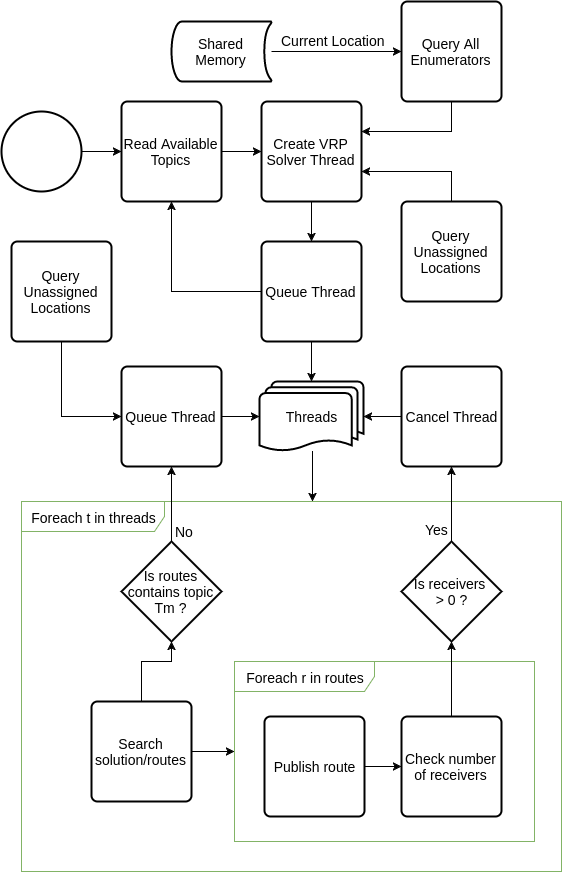
\includegraphics[width=12cm]{Resources/Images/publisher-algorithm}
%	\caption{Publisher Workflow}
%	\label{fig:publisher-algorithm}
%\end{figure}


%-----------------------------------------------------------------------------%
\subsection{\textit{VRP Solver}}
\label{ssec:vrp-solver}
%-----------------------------------------------------------------------------%
\textit{VRP Solver} merupakan sebuah modul yang terdapat di dalam \textit{thread} dan digunakan untuk melakukan kalkulasi rute yang harus dikunjungi oleh petugas. \textit{VRP Solver} dibangun berdasarkan algoritma MDVRP seperti: \textit{tabu search} \cite{cordeau_tabu_1997}, \textit{adaptive large neighborhood search}  \citep{pisinger_general_2007}, \textit{fuzzy logic guided genetic algorithm} \citep{lau_application_2010}, \textit{paralel iterated tabu search} \citep{cordeau_parallel_2012}, \textit{hybrid algorithm combining iterated local search and set partitioning} \citep{subramanian_hybrid_2013}, \textit{hybrid genetic algorithm with adaptive diversity control} \citep{vidal_implicit_2014}, \textit{hybrid granular tabu search} \citep{escobar_hybrid_2014}, dan \textit{cooperative coevolution algorithms} (CoEAs) \citep{de_oliveira_cooperative_2016}. Pada penelitian ini \textit{cooperative coevolutionary algorithms} (CoEAs) dipilih karena menghasilkan rute dengan biaya total yang minimum dan waktu pemrosesan yang relatif singkat dibandingkan algoritma yang lain.


Langkah-langkah yang digunakan dalam implementasi algoritma CoEAs pada \textit{VRPSolver} adalah sebagai berikut:
\begin{enumerate}
\item Definisi masalah \\
Masalah didefinisikan sebagai kumpulan informasi tentang sejumlah $M$ petugas, $N$ lokasi pencacahan, dan $D$ \textit{initial location/depot}. Setiap lokasi $i$, $i \in (D \cup N)$, dilengkapi dengan koordinat lokasi $(x_i, y_i)$. Setiap pasangan lokasi $i$ dan $j$, $i, j \in (D \cup N)$, memiliki biaya sebesar $c_{ij}$ yang merepresentasikan waktu yang diperlukan untuk melakukan perjalanan dari $i$ ke $j$. 

\item Dekomposisi masalah \\
Masalah yang telah didefinisikan sebelumnya akan didekomposisi (dipecah) menjadi beberapa \textit{chunk} submasalah agar proses kalkulasi rute dapat dilakukan secara paralel. 

\item Evolusi \\
Setiap submasalah berisi kombinasi pasangan petugas dan lokasi yang akan dikunjungi (\textit{enumerator-locations pair}). Setiap kombinasi akan mengalami proses evolusi. Pada setiap evolusi yang terjadi, susunan formasi pasangan petugas dan lokasi mengalami perubahan untuk menemukan formasi yang lebih baik. Evolusi terjadi secara iteratif dan setiap iterasi akan menghasilkan formasi baru (\textit{new best formation}). \textit{New best formation} ini akan dievaluasi dengan cara membandingkannya dengan formasi terbaik yang diperoleh dari iterasi sebelumnya (\textit{current best formation}). Jika \textit{new best formation} lebih baik daripada \textit{current best formation}, maka \textit{current best formation} akan diganti dengan \textit{new best formation}. Iterasi akan terus berlangsung sampai dengan solusi/rute yang diperoleh konvergen, yaitu ketika tidak ada lagi \textit{new best formation} yang terbentuk. Formasi yang diperoleh pada akhir keseluruhan iterasi akan dipilih oleh \textit{VRP Solver} sebagai solusi final. 
\end{enumerate}


%-----------------------------------------------------------------------------%
\subsection{\textit{Message Broker}}
\label{ssec:message-broker}
%-----------------------------------------------------------------------------%
\textit{Message broker} merupakan subsistem yang bertanggung jawab dalam menyalurkan (\textit{routing}) pesan dari \textit{publisher} ke \textit{subscriber} dan sebaliknya sesuai dengan topik yang di-\textit{subscribe} \citep{banavar_efficient_1999}. Suatu mekanisme \textit{publish/subscribe} dapat memiliki \textit{single broker} maupun \textit{multi broker}. Pada arsitektur \textit{single broker}, seluruh \textit{subscriber} dan \textit{publisher} terkoneksi pada satu \textit{broker}, sementara pada \textit{multi broker}, \textit{subscriber} maupun \textit{publisher} dapat terkoneksi pada \textit{broker} terdekat. Arsitektur \textit{multi broker} ini disebut juga dengan istilah \textit{distributed publish/subscribe system} \citep{muhl_large-scale_2002}, seperti ilustrasi pada \autoref{fig:pub_sub_distributed_ilustration}. Sistem yang diusulkan akan menerapkan arsitektur terdistribusi agar dapat menangani lokasi pencacahan yang tersebar secara geografis.


\begin{figure}[!]
	\centering
	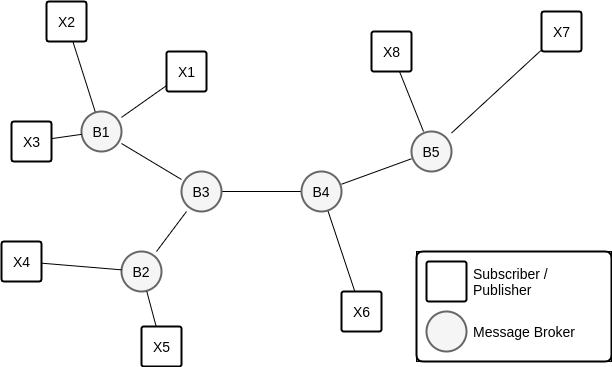
\includegraphics[width=11cm]{Resources/Images/pub_sub_distributed_ilustration}
	\captionsetup{format=hang}
	\caption{Ilustrasi \textit{Publish-Subscribe} terdistribusi}
	\label{fig:pub_sub_distributed_ilustration}
\end{figure}


%#############################################################################%
\begin{comment}
%-----------------------------------------------------------------------------%
\subsection{\textit{Search Algorithm}}
%-----------------------------------------------------------------------------%
Terdapat berbagai variasi algoritma untuk menyelesaikan permasalah TSP maupun VRP, antara lain: genetic algorithm, simmulated annealing, tabu search, particle swarm optimization, harmony search, quantum annealing, greedy 2-opt, dll. Pada pengujian yang dilakukan dengan kasus single-salesman dengan menggunakan 3 (tiga) kriteria: \textit{mean quality}, \textit{dispersion of quality}, dan \textit{time needed to reach the optimum}, simmulated annealing menghasilkan solusi yang paling berkualitas, sementara tabu search merupakan yang paling baik dari sisi performance \citep{antosiewicz_choice_2013}.


%-----------------------------------------------------------------------------%
\subsection{\textit{Greedy Strategy}}
%-----------------------------------------------------------------------------%
Algoritma \textit{greedy} adalah suatu algoritma yang menentukan solusi optimal berdasarkan kondisi saat ini, atau disebut dengan \textit{local optimum}. Algoritma greedy dapat meminimalisir waktu komputasi dalam pencarian solusi global. Pada kasus \textit{travelling salesman problem}, strategi greedy dapat dikatakan dengan "pada setiap tahap, kunjungi kota yang paling dekat dengan lokasi salesman yang belum dikunjungi" \citep{paul_e._black_greedy_2005}. 


Pada metode MTSP, diperoleh lebih dari satu solusi, dimana masing-masing solusi diperbandingkan. Perbandingan dilakukan berdasarkan biaya keseluruhan, dimana solusi dengan biaya terkecil adalah solusi terbaik.


Penentuan solusi terbaik dengan membandingkan biaya keseluruhan tidaklah tepat. \textit{Cost} ditentukan dengan satuan waktu, sementara salah satu komponen utama yang dominan adalah \textit{service time}. Karena \textit{service time} tidak tersedia, maka membandingkan keseluruhan waktu akan menjadi bias. Hipotesis yang ditawarkan adalah membandingkan setiap solusi dengan total biaya untuk lokasi pertama dari masing-masing pencacah saja, karena lokasi pertama tidak terpengaruh dengan \textit{service time}, seperti algoritma dalam Kode \ref{lst:proposed_best_solution_algorithm}.


\begin{listing}
	\caption{Algoritma Solusi Terbaik}
	\label{lst:proposed_best_solution_algorithm}
	\begin{minted}[showspaces=false,breaklines=true]{python}
Let E be all enumerators
Let L be all locations
Run MTSP with enumerators E and locations L
Let S be all solutions from MTSP
Let Cs be an empty dict
For each solution s in S do
	Let R be all routes in solution s
	Let C be 0
	For each route r in R do
		Let J be all jobs in route r
		Let fj be first job in J
		Let cfj be cost of first job fj
		Add C with cjf
	Put C in dict Cs with key solution s
	
Let element in dict Cs with the least value be the best solution
	\end{minted}
\end{listing}


Algoritma \ref{lst:proposed_best_solution_algorithm} merupakan rekomendasi lokasi pertama untuk setiap pencacah. Selanjutnya pencacah dapat melakukan pengumpulan data pada lokasi tersebut sampai selesai, dengan \textit{service time} bervariasi, sehingga waktu selesai pencacahan berbeda-beda antar pencacah. Setiap pencacah yang telah menyelesaikan pengumpulan data, dapat melakukan \textit{subscribe} solusi yang baru kepada \textit{broker}, seperti algoritma pada Kode \ref{lst:proposed_subscribe_solution_algorithm}. Setiap kali broker mendapati adanya \textit{subscribers}, maka \textit{broker} akan mencari solusi baru dengan metode MTSP. Solusi yang dicari hanya menyertakan \textit{subscribers} saja, dan meng-\textit{exclude} lokasi yang telah dikunjungi, seperti algoritma pada Kode \ref{lst:proposed_subscribers_best_solution_algorithm}.


\begin{listing}
	\caption{Algoritma \textit{Subscribe Solution}}
	\label{lst:proposed_subscribe_solution_algorithm}
	\begin{minted}[showspaces=false,breaklines=true]{python}
Let SS be an empty list
For each e in enumerators E do
	If enumerator e has finished enumerating do
		Exclude location l enumerated by e from locations L
		Add e in list of subscribers SS
	\end{minted}
\end{listing}


\begin{listing}
	\caption{Algoritma Solusi Terbaik untuk \textit{Subscribers}}
	\label{lst:proposed_subscribers_best_solution_algorithm}
	\begin{minted}[showspaces=false,breaklines=true]{python}
While locations L is not empty do
	Run MTSP with enumerators SS and locations L
    Let S be all solutions from MTSP
    Let Cs be an empty dict
    For each solution s in S do
	    Let R be all routes in solution s
	    Let C be 0
	    For each route r in R do
		    Let J be all jobs in route r
		    Let fj be first job in J
		    Let cfj be cost of first job fj
		    Add C with cjf
	    Put C in dict Cs with key solution s
	
    Let Bs as element in dict Cs with the least value
    Publish Bs to all subscribers SS
    Set subscribers SS to empty list
	\end{minted}
\end{listing}


%-----------------------------------------------------------------------------%
\subsection{\textit{Publish/Subscribe Paradigm}}
%-----------------------------------------------------------------------------%








\section{Garis Besar Perancangan}

Alur kerja perancangan dimulai dengan dengan mengidentifikasi blok sensus yang akan dilakukan pendataan padanya, serta menentukan jumlah pencacah yang akan digunakan. Kedua permasalahan ini tidak akan dibahas terlalu mendalam dalam penelitian ini. Lokasi pencacahan telah ditentukan dalam fase perancangan sensus dan survei, mengikuti sebuah metodologi tertentu. Sementara jumlah pencacahan juga telah ditentukan, mengikuti jumlah sampel dan berbagai persyaratan tertentu, seperti waktu dan biaya.


Selanjutnya, setiap pencacah akan dialokasikan kepada blok sensus yang akan dicacah dengan menggunakan metode MTSP, sebagaimana diformulasikan oleh \citep{bektas_multiple_2006}, dengan ketentuan setiap pencacah dapat memulai dan mengakhiri pada depot yang berbeda-beda. Setelah model diperoleh, setiap pencacah akan mengunjungi lokasi pertama dari rekomendasi. Setelah selesai kunjungan, lokasi akan disimpan dalam \textit{tabu list} dengan menggunakan metode pub-sub \citep{chen_efficient_2003}. Model baru akan digenerate setiap kali terdapat \textit{request} dari salah satu pencacah. Setiap kali model di-\textit{generate}, \textit{tabu search} \citep{glover_tabu_1989, glover_tabu_1990} yang memanfaatkan \textit{tabu list} akan digunakan untuk memastikan tidak terdapat \textit{conflict}. Setelah model baru selesai di-\textit{generate}, maka mudel akan di-\textit{publish} kepada setiap pencacah yang telah men-\textit{subscribe}.


\begin{figure}[!]
    \centering
    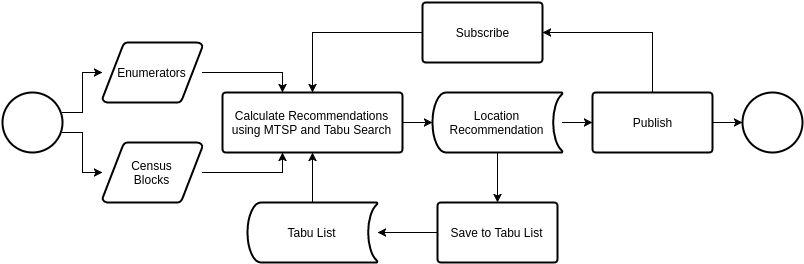
\includegraphics[width=\textwidth]{Resources/Images/design_overview}
    \caption{Garis Besar Sistem Usulan}
    \label{fig:design_overview}
\end{figure}


\section{Penyusunan Rekomendasi}

Pada tahap perumusan rekomendasi, input data yang terdiri dari data pencacah dan data blok sensus akan dioleh menjadi rekomendasi path yang harus dikunjungi. Proses penyusunan rekomendasi menggunakan metode \textit{Multiple Travelling Salesman Problem} (MTSP), yang merupakan pengembangan dari metode klasik \textit{Travelling Salesman Problem} (TSP).


Metode MTSP yang digunakan dalam masalah ini memiliki beberapa \textit{requirements}, antara lain:

\begin{itemize}
\item Jumlah depot \\
MTSP dapat menggunakan lebih dari satu depot, dengan $ m_{j} $ \textit{salesman} untuk setiap depot $ j $. Pada permasalahan ini menggunakan \textit{non-fixed destination}, sehingga pencacahan tidak perlu kembali ke lokasi dimana pencacahan dimulai.
\item Jumlah \textit{salesman} \\
Jumlah \textit{salesman} yang digunakan dapat berupa \textit{fixed number} $ m $, atau dinamis dengan dibatasi jumlah maksimal $ max(m) $. Pada permasalahan ini digunakan \textit{fixed number} $ m $ pencacah.
\item \textit{Fixed charges} \\
Jika jumlah \textit{salesman} dinamis, maka bisa juga masing-masing \textit{salesman} dibatasi dengan sejumlah biaya tertentu. Pada permasalahan ini tidak digunakan \textit{fixed charges}.
\item Waktu kunjungan (\textit{time windows}) \\
\textit{Time windows} merepresentasikan waktu yang dihabiskan selama kunjugan dalam sebuah \textit{node}. Pada kasus ini \textit{time windows} tidak dapat ditentukan karena tidak tersedianya informasi, sehingga dianggap tidak menggunakan \textit{time windows}.
\end{itemize}


Requirements di atas, secara global dapat disederhanakan dalam tabel-tebel berikut. Tabel \ref{tbl:enumerators_overview} menunjukkan rancangan pencacah beserta koordinat depot-nya, sementara Tabel \ref{tbl:census_blocks} menunjukkan rancangan blok sensus beserta koordinat dan \textit{time windows}-nya. Dalam fakta lapangan, jarak antara satu blok sensus dengan blok sensus yang lain tidaklah setara. Bisa jadi secara koordinat memiliki jarak yang berdekatan, tetapi secara akses tidaklah mudah. Untuk itu diperlukan sebuah tabel tambahan, yaitu tabel \textit{cost-matrix}, sebagaimana Tabel \ref{tbl:cost_matrix}. \textit{Cost} yang dimaksud disini adalah segala metrik yang dapat digunakan sebagai penimbang (\textit{weight}), misalnya: biaya, jarak, atau waktu tempuh.


\begin{table}[]
\centering
\caption{Table Pencacah}
\label{tbl:enumerators_overview}
\begin{tabular}{@{}lcc@{}}
\toprule
\multirow{2}{*}{Pencacah} & \multicolumn{2}{l}{\textit{Depot Coordinate}} \\ \cmidrule(l){2-3} 
                          & X                 & Y                \\ \midrule
Pencacah 1                & 20.0              & 20.0             \\
Pencacah 2                & 20.0              & 20.0             \\
Pencacah 3                & 30.0              & 40.0             \\
Pencacah 4                & 30.0              & 40.0             \\
...                       &                   &                  \\
Pencacah m                & x                 & y                \\ \bottomrule
\end{tabular}
\end{table}


\begin{table}[]
\centering
\caption{Tabel Blok Sensus}
\label{tbl:census_blocks}
\begin{tabular}{@{}lccc@{}}
\toprule
\multirow{2}{*}{Blok Sensus} & \multicolumn{2}{c}{Koordinat Lokasi} & \multirow{2}{*}{Time Windows} \\ \cmidrule(lr){2-3}
                             & X                 & Y                &                               \\ \midrule
001B                         & 62.0              & 63.0             & 0                             \\
002B                         & 63.0              & 69.0             & 0                             \\
003B                         & 46.0              & 10.0             & 0                             \\
004B                         & 61.0              & 33.0             & 0                             \\
...                          &                   &                  &                               \\
n                            & x                 & y                & 0                             \\ \bottomrule
\end{tabular}
\end{table}


\begin{table}[]
\centering
\caption{Table \textit{Cost-Matrix}}
\label{tbl:cost_matrix}
\begin{tabular}{@{}|c|c|c|c|c|c|c|@{}}
\toprule
        & 001B & 002B & 003B & 004B & ... & BS ke-n \\ \midrule
001B    & -    & 5    & 2    & 2    &     & ...     \\ \midrule
002B    &      & -    & 4    & 2    &     & ...     \\ \midrule
003B    &      &      & -    & 7    &     & ...     \\ \midrule
004B    &      &      &      & -    &     & ...     \\ \midrule
...     &      &      &      &      & -   & ...     \\ \midrule
BS ke-n &      &      &      &      &     & -       \\ \bottomrule
\end{tabular}
\end{table}


Tabel \textit{cost-matrix}, selain dapat didefinisikan secara manual (berdasarkan hasil survei atau perkiraan \textit{subject matter}), dapat juga didekati dengan menggunakan Google Directions API \citep{google_google_2016}. \textit{Request} yang digunakan menggunakan standar REST API, sementara \textit{response} yang ditampilkan dalam format JSON. Listing \ref{lst:google_direction_api_request} menunjukkan contoh \textit{request}, dan Gambar \ref{fig:google_direction_api_response} menunjukkan contoh \textit{response} dari Google Direction API.








%Gambar \ref{fig:mtsp_solution_example} berikut menunjukkan hasil rekomendasi dengan MTSP.
%
%
%\begin{figure}[!]
%    \centering
%    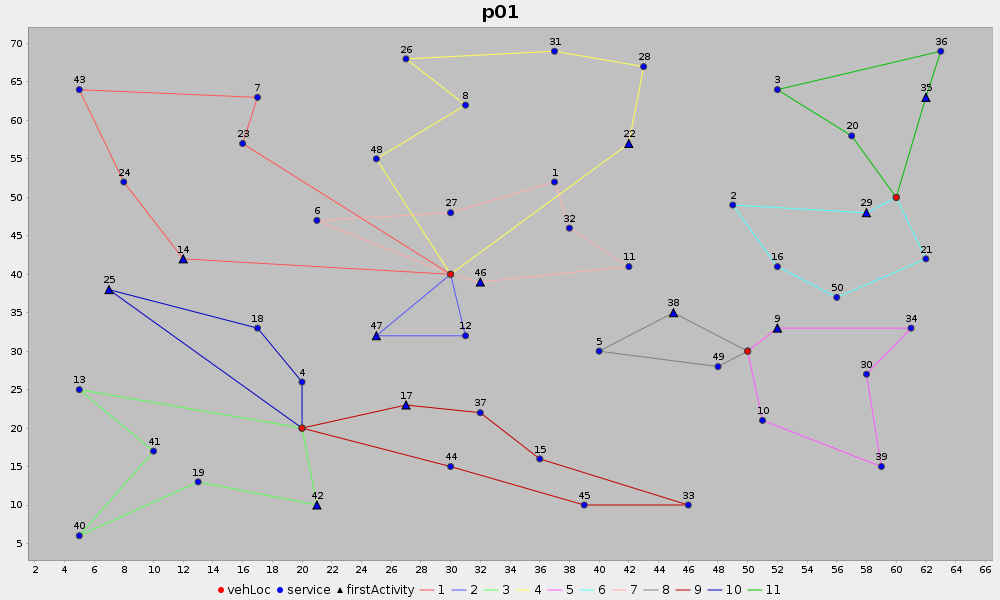
\includegraphics[width=\textwidth]{Resources/Images/mtsp_solution_example}
%    \caption{Contoh Hasil Rekomendasi}
%    \label{fig:mtsp_solution_example}
%\end{figure}


\section{Penyusunan \textit{Conflict Resolution}}


\section{\textit{Publish-Subscribe} Rekomendasi}
\end{comment}
%#############################################################################%

%-----------------------------------------------------------------------------%
\chapter{\babLima}
%-----------------------------------------------------------------------------%
\todo{Tambahkan kata-kata pengantar bab 5 disini.}


%-----------------------------------------------------------------------------%
\section{Mengubah Tampilan Teks}
%-----------------------------------------------------------------------------%
Beberapa perintah yang dapat digunakan untuk mengubah tampilan adalah: 
\begin{itemize}
	\item \bslash f \\
		Merupakan alias untuk perintah \bslash textit, contoh 
		\f{contoh hasil tulisan}.
	\item \bslash bi \\
		\bi{Contoh hasil tulisan}.
	\item \bslash bo \\
		\bo{Contoh hasil tulisan}.
	\item \bslash m \\
		\m{Contoh hasil tulisan}.
	\item \bslash mc \\
		\mc{Contoh hasil tulisan}.
	\item \bslash code \\ 
		\code{Contoh hasil tulisan}.
\end{itemize}


%-----------------------------------------------------------------------------%
\section{Memberikan Catatan}
%-----------------------------------------------------------------------------%
Ada dua perintah untuk memberikan catatan penulisan dalam dokumen yang Anda 
kerjakan, yaitu: 
\begin{itemize}
	\item \bslash todo \\
		Contoh: \\ \todo{Contoh bentuk todo.}
	\item \bslash todoCite \\ 
		Contoh: \todoCite
\end{itemize}


%-----------------------------------------------------------------------------%
\section{Menambah Isi Daftar Isi}
%-----------------------------------------------------------------------------%
Terkadang ada kebutuhan untuk memasukan kata-kata tertentu kedalam Daftar Isi. 
Perintah \bslash addChapter dapat digunakan untuk judul bab dalam Daftar isi. 
Contohnya dapat dilihat pada berkas thesis.tex.


%-----------------------------------------------------------------------------%
\section{Memasukan PDF}
%-----------------------------------------------------------------------------%
Untuk memasukan PDF dapat menggunakan perintah \bslash inpdf yang menerima satu 
buah argumen. Argumen ini berisi nama berkas yang akan digabungkan dalam 
laporan. PDF yang dimasukan degnan cara ini akan memiliki header dan footer 
seperti pada halaman lainnya. 

\inpdf{include}

Cara lain untuk memasukan PDF adalah dengan menggunakan perintah \bslash putpdf 
dengan satu argumen yang berisi nama berkas pdf. Berbeda dengan perintah 
sebelumnya, PDF yang dimasukan dengan cara ini tidak akan memiliki footer atau 
header seperti pada halaman lainnya. 

\putpdf{include}


%-----------------------------------------------------------------------------%
\section{Membuat Perintah Baru}
%-----------------------------------------------------------------------------%
Ada dua perintah yang dapat digunakan untuk membuat perintah baru, yaitu: 
\begin{itemize}
	\item \bslash Var \\
		Digunakan untuk membuat perintah baru, namun setiap kata yang diberikan
		akan diproses dahulu menjadi huruf kapital. 
		Contoh jika perintahnya adalah \bslash Var\{adalah\} makan ketika 
		perintah \bslash Var dipanggil, yang akan muncul adalah ADALAH. 
	\item \bslash var \\
		Digunakan untuk membuat perintah atau baru. 
\end{itemize}


%---------------------------------------------------------------
\chapter{\kesimpulan}
%---------------------------------------------------------------
%\todo{Tambahkan kesimpulan dan saran terkait dengan perkerjaan 
%	yang dilakukan.}


%---------------------------------------------------------------
\section{Kesimpulan}
%---------------------------------------------------------------
Berdasarkan hasil pengujian, diperoleh kesimpulan sebagai berikut:

\begin{enumerate}
	\item Pada permasalahan MDVRP yang tidak mempertimbangkan \textit{service time}, diperoleh hasil bahwasannya sistem usulan yang menggunakan algoritma MDVRP berbasis CoEAs yang dikombinasikan dengan mekanisme Publish/Subscribe menghasilkan total waktu 80 persen lebih buruk dari program pembanding yang menggunakan algoritma MDVRP berbasis CoEAs tanpa mekanisme Publish/Subscribe. Sementara dari sisi \textit{standar deviasi}, sistem usulan menghasilkan 80 persen lebih baik dari aplikasi pembanding. Dengan demikian dapat disimpulkan algoritma MDVRP berbasis CoEAs dengan mekanisme Publish/Subscribe menghasilkan total waktu yang lebih merata antar rute yang dihasilkan, sementara algoritma MDVRP berbasis CoEAs tanpa mekanisme Publish/Subscribe menghasilkan total waktu yang lebih efisien.
	\item Pada permasalahan MDVRP yang mempertimbangkan \textit{service time}, dengan menggunakan data Cordeau PO1 diperoleh hasil total waktu yang dihasilkan dari sistem usulan 6,25 persen lebih buruk dari aplikasi pembanding, tetapi 68,83 persen lebih baik dari sisi standar deviasi. Sementara pada pengujian dengan menggunakan data lapangan, sistem usulan lebih buruk 8,25 persen dibandingkan program pembanding, tetapi 59,11 persen dari sisi standar deviasi. Pada pengujian kondisi normal, dapat disimpulkan algoritma MDVRP berbasis CoEAs dengan mekanisme Publish/Subscribe lebih sesuai digunakan pada permasalahan rekomendasi lokasi pencacahan karena menghasilkan total waktu yang lebih merata antar pencacah.
	\item Pada permasalahan MDVRP yang mempertimbangkan \textit{service time} dan terdapat \textit{delay} dalam jaringan, pada pengujian dengan menggunakan data lapangan diperoleh hasil bahwasannya sistem usulan 4,83 persen lebih buruk dari sisi total waktu, tetapi 3,62 persen lebih baik dari sisi standar deviasi. Pada pengujian kondisi dimana terdapat \textit{delay} pada koneksi, dapat disimpulkan bahwa meskipun memiliki perbedaan yang tipis, algoritma MDVRP berbasis CoEAs dengan mekanisme Publish/Subscribe masih lebih sesuai digunakan pada permasalahan rekomendasi lokasi pencacahan karena menghasilkan total waktu yang lebih merata antar pencacah.
	\item Pada permasalahan MDVRP yang mempertimbangkan \textit{service time} dan terdapat \textit{packet loss} dalam jaringan, pada pengujian dengan menggunakan data lapangan diperoleh hasil bahwasannya sistem usulan 12,79 persen lebih buruk dari sisi total waktu, tetapi 36,14 persen lebih baik dari sisi standar deviasi. Pada pengujian kondisi dimana terdapat \textit{packet loss} pada koneksi, dapat disimpulkan bahwa algoritma MDVRP berbasis CoEAs dengan mekanisme Publish/Subscribe lebih sesuai digunakan pada permasalahan rekomendasi lokasi pencacahan karena menghasilkan total waktu yang lebih merata antar pencacah.
\end{enumerate}


%---------------------------------------------------------------
\section{Saran}
%---------------------------------------------------------------
Dari penelitian ini, saran yang diberikan untuk penelitian selanjutnya sebagai berikut:

\begin{enumerate}
	\item Mengkaji mekanisme komunikasi yang digunakan, misalnya dengan membandingkan dengan mekanisme Request/Reply dan Push/Pull untuk mendapatkan mekanisme komunikasi yang paling tepat.
	\item Mengkaji parameter yang dapat digunakan dalam VRP Solver yaitu lama waktu eksekusi dan lama waktu dimana tidak ada perubahan solusi terbaik, sehingga diperoleh waktu eksekusi yang paling optimal.
	\item Mengkasi penggunaan algoritma MDVRP yang lain, misalnya Tabu Search, Particle Swarm Optimization, dan lain lain, sehingga diperoleh algoritma MDVRP yang paling sesuai.
\end{enumerate}


%
% Daftar Pustaka
%
% Daftar Pustaka 
% 

% 
% Tambahkan pustaka yang digunakan setelah perintah berikut. 
% 
\addcontentsline{toc}{chapter}{\bibname}
\bibliography{\bibFile}



%
% Lampiran 
%
\begin{appendix}
	%
% @author  Andreas Febrian
% @version 1.00 
% 
% Hanya sebuah pembatas bertuliskan LAMPIRAN ditengah halaman. 
% 

\begin{titlepage}
	\centering 
	\vspace*{6cm}
	\noindent \Huge{LAMPIRAN}
	\addChapter{LAMPIRAN}
\end{titlepage}
	\setcounter{page}{2}
	%-----------------------------------------------------------------------------%
\addChapter{LAMPIRAN 1}
\chapter*{Lampiran 1}
%-----------------------------------------------------------------------------%


\begin{longtable}[h]{lcc}
	\caption{Lokasi Pencacahan}
	\label{tbl:enumeration_locations_full}\\
	\toprule
		& \multicolumn{2}{c}{Koordinat}\\
	\cmidrule{2-3}
		& Latitude & Longitude\\ 
	\midrule
	\endfirsthead
	\toprule
		& \multicolumn{2}{c}{Koordinat}\\
	\cmidrule{2-3}
		& Latitude & Longitude\\ 
	\midrule
	\endhead
	\bottomrule
	\endfoot
		1302011001 & -2.3504 & 101.1434\\ 
		1302011002 & -2.4233 & 101.0285\\ 
		1302011003 & -2.3798 & 101.0427\\ 
		1302011004 & -2.3884 & 101.049\\ 
		1302011005 & -2.3936 & 101.0546\\ 
		1302011006 & -2.3985 & 101.0546\\ 
		1302011007 & -2.4171 & 101.101\\ 
		1302011008 & -2.3905 & 101.1214\\ 
		1302011009 & -2.3819 & 101.1005\\ 
		1302011010 & -2.3593 & 101.1404\\ 
		1302012001 & -2.2494 & 101.1331\\ 
		1302012002 & -2.2758 & 101.1432\\ 
		1302012003 & -2.199 & 101.1188\\ 
		1302012004 & -2.2655 & 101.1052\\ 
		1302012005 & -2.3155 & 101.1678\\ 
		1302012006 & -2.2666 & 101.14\\ 
		1302012007 & -2.219 & 101.1193\\ 
		1302012008 & -2.1971 & 101.1206\\ 
		1302012009 & -2.2717 & 101.0965\\ 
		1302012010 & -2.2883 & 101.0858\\ 
		1302020001 & -2.1806 & 101.0609\\ 
		1302020003 & -2.1623 & 101.0819\\ 
		1302020005 & -2.1569 & 101.0816\\ 
		1302020006 & -2.1225 & 101.0687\\ 
		1302020009 & -2.1692 & 101.0609\\ 
		1302020010 & -2.1797 & 101.0686\\ 
		1302020011 & -2.1648 & 101.0727\\ 
		1302020015 & -2.1549 & 101.0811\\ 
		1302020016 & -2.139 & 101.0794\\ 
		1302020017 & -2.1022 & 101.0522\\ 
		1302021001 & -2.1844 & 101.092\\ 
		1302021002 & -2.1479 & 101.089\\ 
		1302021003 & -2.1454 & 101.0995\\ 
		1302021004 & -2.13 & 101.1843\\ 
		1302021005 & -2.1845 & 101.0959\\ 
		1302021006 & -2.1562 & 101.0844\\ 
		1302021007 & -2.1419 & 101.0936\\ 
		1302021008 & -2.1386 & 101.0936\\ 
		1302021009 & -2.1253 & 101.1184\\ 
		1302021010 & -2.1252 & 101.1244\\ 
		1302030001 & -2 & 101\\ 
		1302030002 & -2.0702 & 100.9105\\ 
		1302030003 & -2.0674 & 100.9152\\ 
		1302030004 & -2.0742 & 100.9401\\ 
		1302030005 & -2.0509 & 101.021\\ 
		1302030006 & -2.0517 & 100.9653\\ 
		1302030009 & -2.0639 & 100.9521\\ 
		1302030010 & -2.0971 & 100.9122\\ 
		1302030012 & -2.0689 & 100.9247\\ 
		1302030014 & -2.0444 & 100.9885\\ 
		1302031001 & -2.0419 & 100.9542\\ 
		1302031002 & -1.9875 & 100.9696\\ 
		1302031003 & -2.0247 & 100.8822\\ 
		1302031004 & -2.0453 & 100.9136\\ 
		1302031005 & -2.0018 & 100.9542\\ 
		1302031006 & -2.0263 & 100.9451\\ 
		1302031007 & -1.9871 & 100.9885\\ 
		1302031008 & -1.9924 & 100.915\\ 
		1302031009 & -1.9808 & 100.9341\\ 
		1302031010 & -1.9872 & 100.9383\\ 
		1302040001 & -1.9199 & 100.8821\\ 
		1302040002 & -1.8856 & 100.8658\\ 
		1302040003 & -1.8778 & 100.8826\\ 
		1302040004 & -1.8805 & 100.8762\\ 
		1302040005 & -1.8445 & 100.8816\\ 
		1302040006 & -1.8478 & 100.8707\\ 
		1302040007 & -1.8702 & 100.8529\\ 
		1302040008 & -1.9579 & 100.8801\\ 
		1302040009 & -1.9318 & 100.8799\\ 
		1302040010 & -1.9334 & 100.8927\\ 
		1302040011 & -1.9617 & 100.9195\\ 
		1302040012 & -1.9165 & 100.9383\\ 
		1302040013 & -1.9235 & 100.8944\\ 
		1302040014 & -1.921 & 100.921\\ 
		1302040015 & -1.8986 & 100.9037\\ 
		1302040016 & -1.8898 & 100.8451\\ 
		1302050001 & -1.84413 & 100.84115\\ 
		1302050002 & -1.79495 & 100.83736\\ 
		1302050003 & -1.83965 & 100.81264\\ 
		1302050004 & -1.82058 & 100.8397\\ 
		1302050005 & -1.81249 & 100.79719\\ 
		1302050006 & -1.80491 & 100.86681\\ 
		1302050007 & -1.78067 & 100.842\\ 
		1302050008 & -1.78258 & 100.81757\\ 
		1302050009 & -1.78144 & 100.78438\\ 
		1302050010 & -1.76208 & 100.798\\ 
		1302060001 & -1.7302 & 100.7376\\ 
		1302060002 & -1.6709 & 100.7568\\ 
		1302060003 & -1.7425 & 100.7479\\ 
		1302060004 & -1.7161 & 100.7683\\ 
		1302060005 & -1.7016 & 100.7639\\ 
		1302060006 & -1.7086 & 100.7306\\ 
		1302060007 & -1.6942 & 100.7104\\ 
		1302060008 & -1.6532 & 100.7544\\ 
		1302060009 & -1.6732 & 100.79\\ 
		1302070001 & -1.6301 & 100.6598\\ 
		1302070002 & -1.5663 & 100.6457\\ 
		1302070003 & -1.5478 & 100.6343\\ 
		1302070004 & -1.6138 & 100.7063\\ 
		1302070005 & -1.5816 & 100.6553\\ 
		1302070006 & -1.5707 & 100.6505\\ 
		1302070007 & -1.5708 & 100.6792\\ 
		1302070008 & -1.5661 & 100.6856\\ 
		1302070009 & -1.5181 & 100.6882\\ 
		1302070010 & -1.4783 & 100.7141\\ 
		1302070011 & -1.5654 & 100.6407\\ 
		1302070012 & -1.5301 & 100.6219\\ 
		1302080001 & -1.4422 & 100.6008\\ 
		1302080002 & -1.4336 & 100.6365\\ 
		1302080003 & -1.4951 & 100.6282\\ 
		1302080004 & -1.4763 & 100.609\\ 
		1302080005 & -1.4417 & 100.591\\ 
		1302080006 & -1.4448 & 100.6285\\ 
		1302080007 & -1.4431 & 100.6419\\ 
		1302080008 & -1.4129 & 100.6483\\ 
		1302080009 & -1.4932 & 100.635\\ 
		1302090001 & -1.3322 & 100.5698\\ 
		1302090002 & -1.3486 & 100.5752\\ 
		1302090003 & -1.2772 & 100.584\\ 
		1302090004 & -1.31897 & 100.6105\\ 
		1302090005 & -1.3351 & 100.5844\\ 
		1302090006 & -1.3089 & 100.5499\\ 
		1302090007 & -1.3492 & 100.5696\\ 
		1302090008 & -1.3501 & 100.5848\\ 
		1302090009 & -1.2697 & 100.5623\\ 
		1302090010 & -1.2672 & 100.5537\\ 
		1302090011 & -1.26964 & 100.5678\\ 
		1302090012 & -1.2822 & 100.5622\\ 
		1302090013 & -1.28608 & 100.5845\\ 
		1302090014 & -1.2764 & 100.581\\ 
		1302090015 & -1.2717 & 100.5755\\ 
		1302090016 & -1.2721 & 100.5982\\ 
		1302090017 & -1.2664 & 100.6043\\ 
		1302090018 & -1.2616 & 100.6097\\ 
		1302090019 & -1.3015 & 100.6235\\ 
		1302090020 & -1.2984 & 100.6368\\ 
		1302100001 & -1.3054 & 100.51371\\ 
		1302100002 & -1.23265 & 100.54314\\ 
		1302100003 & -1.237388 &  100.537983\\ 
		1302100004 & -1.28778 & 100.53125\\ 
		1302100005 & -1.2977 & 100.49147\\ 
		1302100006 & -1.29728 & 100.50949\\ 
		1302100007 & -1.29145 & 100.50856\\ 
		1302100008 & -1.28337 & 100.50654\\ 
		1302100009 & -1.25761 & 100.51635\\ 
		1302100010 & -1.175763 &  100.610463\\ 
		1302100011 & -1.160535 &  100.661145\\ 
		1302100012 & -1.22142 & 100.54697\\ 
		1302100013 & -1.22142 & 100.54697\\ 
		1302100014 & -1.21365 & 100.658232\\ 
		1302100015 & -1.29294 & 100.53711\\ 
		1302100016 & -1.273358 &  100.545953\\ 
		1302100017 & -1.29637 & 100.52366\\ 
		1302101001 & -1.19533 & 100.58535\\ 
		1302101002 & -1.17243 & 100.61153\\ 
		1302101003 & -1.1503 & 100.62934\\ 
		1302101004 & -1.15408 & 100.66563\\ 
		1302101005 & -1.19831 & 100.58078\\ 
		1302101006 & -1.1347577 & 100.674752\\ 
		1302110001 & -1.2748 & 100.4753\\ 
		1302110002 & -1.2559 & 100.458\\ 
		1302110003 & -1.2475 & 100.4745\\ 
		1302110004 & -1.2384 & 100.4869\\ 
		1302110005 & -1.2156 & 100.5016\\ 
		1302110006 & -1.1374 & 100.491\\ 
		1302110007 & -1.146 & 100.3814\\ 
		1302110008 & -1.0751 & 100.444\\ 
		1302110009 & -1.0664 & 100.5103\\ 
		1302110010 & -1.2671 & 100.4745\\ 
		1302110011 & -1.1919 & 100.4344\\ 
		1302110012 & -1.1655 & 100.5009\\ 
		1302110013 & -1.2544 & 100.4658\\ 
		1302110014 & -1.2623 & 100.4618\\ 
		1302110015 & -1.2513 & 100.4495\\ 
		1302110016 & -1.1792 & 100.4062\\ 
		1302110017 & -1.2161 & 100.4654\\ 
		1302110018 & -1.2387 & 100.4853\\ 
		1302110019 & -1.2387 & 100.4853\\ 
		1302110020 & -1.1408 & 100.4938\\ 
		1302110021 & -1.0883 & 100.4652\\ 
		1302110022 & -1.0886 & 100.489\\ 
		1302110023 & -1.1523 & 100.4978\\
\end{longtable}
	%-----------------------------------------------------------------------------%
\addChapter{LAMPIRAN 2}
\chapter*{Lampiran 2}
%-----------------------------------------------------------------------------%


\begin{longtable}[h]{llcc}
	\caption{Matriks Jarak dan Waktu Tempuh}
	\label{tbl:distance_duration_matrix_full}\\
	\toprule
		Lokasi A & Lokasi B & Jarak & Waktu Tempuh\\ 
	\midrule
	\endfirsthead
	\toprule
		Lokasi A & Lokasi B & Jarak & Waktu Tempuh\\ 
	\midrule
	\endhead
	\bottomrule
	\endfoot
		1302021001 & 1302021003 & 11119 & 1055\\
		1302021001 & 1302021002 & 9373 & 868\\
		1302021001 & 1302021005 & 490 & 38\\
		1302021001 & 1302021004 & 22760 & 2044\\
		1302021001 & 1302021007 & 10228 & 950\\
		1302021001 & 1302021006 & 8322 & 761\\
		1302021001 & 1302021009 & 13634 & 1256\\
		1302021001 & 1302021008 & 10720 & 1045\\
		1302021001 & 1302110019 & 164502 & 15267\\
		1302021001 & 1302110018 & 164502 & 15267\\
		1302021001 & 1302100016 & 154841 & 15001\\
		1302021001 & 1302110015 & 165317 & 15424\\
		1302021001 & 1302110014 & 165350 & 15435\\
		1302021001 & 1302110017 & 166862 & 15718\\
		1302021001 & 1302090020 & 152864 & 14784\\
		1302021001 & 1302110011 & 173310 & 16994\\
		1302021001 & 1302110010 & 160346 & 14854\\
		1302021001 & 1302110013 & 162906 & 15118\\
		1302021001 & 1302110012 & 174056 & 16027\\
		1302021001 & 1302012003 & 4104 & 323\\
		1302021001 & 1302012002 & 14598 & 1281\\
		1302021001 & 1302012001 & 11146 & 874\\
		1302021001 & 1302012007 & 6065 & 471\\
		1302021001 & 1302012006 & 13380 & 1133\\
		1302021001 & 1302012005 & 21342 & 1769\\
		1302021001 & 1302012004 & 16384 & 1553\\
		1302021001 & 1302012009 & 18039 & 1826\\
		1302021001 & 1302012008 & 4405 & 354\\
		1302021001 & 1302110020 & 177081 & 16290\\
		1302021001 & 1302110021 & 185436 & 16923\\
		1302021001 & 1302110022 & 183419 & 16815\\
		1302021001 & 1302110023 & 175593 & 16139\\
		1302021001 & 1302030009 & 33670 & 3262\\
		1302021001 & 1302030003 & 38475 & 3747\\
		1302021001 & 1302030002 & 39142 & 3839\\
		1302021001 & 1302030001 & 46459 & 4846\\
		1302021001 & 1302070012 & 110355 & 10562\\
		1302021001 & 1302030006 & 31816 & 3035\\
		1302021001 & 1302030005 & 24325 & 2349\\
		1302021001 & 1302030004 & 35523 & 3438\\
		1302021001 & 1302090008 & 141381 & 13171\\
		1302021001 & 1302110016 & 185134 & 19362\\
		1302021001 & 1302011002 & 45912 & 4574\\
		1302021001 & 1302011003 & 42847 & 4141\\
		1302021001 & 1302011001 & 26534 & 2175\\
		1302021001 & 1302011006 & 40836 & 3964\\
		1302021001 & 1302011007 & 37279 & 3468\\
		1302021001 & 1302011004 & 41296 & 3956\\
		1302021001 & 1302011005 & 40091 & 3794\\
		1302021001 & 1302011008 & 32566 & 2887\\
		1302021001 & 1302011009 & 35049 & 3189\\
		1302021001 & 1302100007 & 154576 & 14485\\
		1302021001 & 1302100006 & 153915 & 14420\\
		1302021001 & 1302100005 & 156127 & 14505\\
		1302021001 & 1302100004 & 151721 & 14443\\
		1302021001 & 1302100003 & 161820 & 15435\\
		1302021001 & 1302100001 & 153358 & 14275\\
		1302021001 & 1302011010 & 27604 & 2258\\
		1302021001 & 1302101005 & 168499 & 15906\\
		1302021001 & 1302110004 & 164587 & 15262\\
		1302021001 & 1302030014 & 28778 & 2722\\
		1302021001 & 1302100010 & 173313 & 16573\\
		1302021001 & 1302100011 & 181730 & 17610\\
		1302021001 & 1302030010 & 42091 & 4225\\
		1302021001 & 1302100012 & 163409 & 15358\\
		1302021001 & 1302101001 & 169104 & 15981\\
		1302021001 & 1302101002 & 173742 & 16397\\
		1302021001 & 1302070004 & 102532 & 9959\\
		1302021001 & 1302031008 & 42879 & 4526\\
		1302021001 & 1302030012 & 37379 & 3619\\
		1302021001 & 1302101006 & 184913 & 17920\\
		1302021001 & 1302031004 & 42311 & 4178\\
		1302021001 & 1302031005 & 39103 & 3896\\
		1302021001 & 1302031006 & 36847 & 3708\\
		1302021001 & 1302031007 & 45966 & 4715\\
		1302021001 & 1302031001 & 33985 & 3380\\
		1302021001 & 1302031002 & 42839 & 4281\\
		1302021001 & 1302031003 & 46237 & 4714\\
		1302021001 & 1302020009 & 5217 & 388\\
		1302021001 & 1302060001 & 82918 & 8084\\
		1302021001 & 1302070001 & 97458 & 9416\\
		1302021001 & 1302101004 & 182639 & 17546\\
		1302021001 & 1302020003 & 7751 & 723\\
		1302021001 & 1302020001 & 3817 & 282\\
		1302021001 & 1302020006 & 12925 & 1277\\
		1302021001 & 1302020005 & 8125 & 730\\
		1302021001 & 1302090012 & 152093 & 14315\\
		1302021001 & 1302090013 & 152433 & 14480\\
		1302021001 & 1302090010 & 156024 & 14914\\
		1302021001 & 1302090011 & 157576 & 15146\\
		1302021001 & 1302090016 & 153950 & 14694\\
		1302021001 & 1302090017 & 153950 & 14694\\
		1302021001 & 1302090014 & 152765 & 14501\\
		1302021001 & 1302090015 & 153430 & 14578\\
		1302021001 & 1302090018 & 153950 & 14694\\
		1302021001 & 1302090019 & 151246 & 14525\\
		1302021001 & 1302080001 & 123861 & 11657\\
		1302021001 & 1302080002 & 128941 & 12358\\
		1302021001 & 1302080003 & 115299 & 10956\\
		1302021001 & 1302080004 & 119160 & 11249\\
		1302021001 & 1302080005 & 125015 & 11788\\
		1302021001 & 1302080006 & 127963 & 12194\\
		1302021001 & 1302080007 & 129277 & 12377\\
		1302021001 & 1302080008 & 131826 & 12811\\
		1302021001 & 1302080009 & 115906 & 11149\\
		1302021001 & 1302031010 & 41588 & 4161\\
		1302021001 & 1302070009 & 114721 & 11664\\
		1302021001 & 1302070008 & 108505 & 10673\\
		1302021001 & 1302070007 & 107638 & 10541\\
		1302021001 & 1302070006 & 105448 & 10298\\
		1302021001 & 1302070005 & 104371 & 10162\\
		1302021001 & 1302060009 & 90633 & 9379\\
		1302021001 & 1302070003 & 107439 & 10315\\
		1302021001 & 1302070002 & 105646 & 10299\\
		1302021001 & 1302050010 & 78399 & 7882\\
		1302021001 & 1302100017 & 153263 & 14330\\
		1302021001 & 1302060006 & 86175 & 8543\\
		1302021001 & 1302101003 & 177923 & 16790\\
		1302021001 & 1302060008 & 94507 & 9384\\
		1302021001 & 1302060007 & 88255 & 8590\\
		1302021001 & 1302020011 & 6687 & 551\\
		1302021001 & 1302020010 & 2897 & 212\\
		1302021001 & 1302060004 & 84615 & 8419\\
		1302021001 & 1302060005 & 86516 & 8700\\
		1302021001 & 1302020015 & 8262 & 728\\
		1302021001 & 1302060003 & 81116 & 7907\\
		1302021001 & 1302020017 & 16084 & 1551\\
		1302021001 & 1302020016 & 10354 & 1027\\
		1302021001 & 1302090001 & 144078 & 13461\\
		1302021001 & 1302090003 & 152497 & 14469\\
		1302021001 & 1302090002 & 141091 & 13161\\
		1302021001 & 1302090005 & 143475 & 13499\\
		1302021001 & 1302090004 & 148255 & 14046\\
		1302021001 & 1302090007 & 141471 & 13220\\
		1302021001 & 1302090006 & 148131 & 13867\\
		1302021001 & 1302090009 & 154973 & 14757\\
		1302021001 & 1302060002 & 94791 & 9437\\
		1302021001 & 1302070010 & 120450 & 12582\\
		1302021001 & 1302040008 & 52180 & 5114\\
		1302021001 & 1302040009 & 52322 & 5209\\
		1302021001 & 1302070011 & 105323 & 10144\\
		1302021001 & 1302040004 & 57662 & 6010\\
		1302021001 & 1302040005 & 64078 & 6688\\
		1302021001 & 1302040006 & 62655 & 6506\\
		1302021001 & 1302040007 & 58974 & 6007\\
		1302021001 & 1302100013 & 163409 & 15358\\
		1302021001 & 1302040001 & 51993 & 5214\\
		1302021001 & 1302040002 & 56386 & 5755\\
		1302021001 & 1302040003 & 58481 & 6142\\
		1302021001 & 1302021010 & 14349 & 1322\\
		1302021001 & 1302050009 & 75019 & 7431\\
		1302021001 & 1302050008 & 72509 & 7397\\
		1302021001 & 1302100009 & 158724 & 14929\\
		1302021001 & 1302100008 & 155647 & 14601\\
		1302021001 & 1302050005 & 69478 & 7012\\
		1302021001 & 1302050004 & 64789 & 6565\\
		1302021001 & 1302050007 & 70297 & 7285\\
		1302021001 & 1302050006 & 68547 & 7055\\
		1302021001 & 1302050001 & 62377 & 6309\\
		1302021001 & 1302100002 & 162600 & 15277\\
		1302021001 & 1302050003 & 65613 & 6570\\
		1302021001 & 1302050002 & 69757 & 7144\\
		1302021001 & 1302110008 & 188509 & 17170\\
		1302021001 & 1302110009 & 187682 & 17285\\
		1302021001 & 1302110006 & 177484 & 16299\\
		1302021001 & 1302110007 & 206195 & 20723\\
		1302021001 & 1302100014 & 183350 & 17664\\
		1302021001 & 1302110005 & 167700 & 15513\\
		1302021001 & 1302110002 & 163791 & 15225\\
		1302021001 & 1302110003 & 162881 & 15111\\
		1302021001 & 1302110001 & 159352 & 14768\\
		1302021001 & 1302031009 & 42406 & 4259\\
		1302021001 & 1302040013 & 51548 & 5179\\
		1302021001 & 1302040012 & 54170 & 5567\\
		1302021001 & 1302040011 & 45452 & 4488\\
		1302021001 & 1302040010 & 50328 & 4977\\
		1302021001 & 1302040016 & 58378 & 5890\\
		1302021001 & 1302040015 & 56854 & 6045\\
		1302021001 & 1302040014 & 52527 & 5304\\
		1302021001 & 1302100015 & 150603 & 14266\\
		1302021001 & 1302012010 & 21034 & 2254\\
		1302021003 & 1302021002 & 1746 & 186\\
		1302021003 & 1302021005 & 11610 & 1068\\
		1302021003 & 1302021004 & 13139 & 1166\\
		1302021003 & 1302021007 & 891 & 104\\
		1302021003 & 1302021006 & 2797 & 294\\
		1302021003 & 1302021009 & 4013 & 378\\
		1302021003 & 1302021008 & 1279 & 193\\
		1302021003 & 1302110019 & 159436 & 14964\\
		1302021003 & 1302110018 & 159436 & 14964\\
		1302021003 & 1302100016 & 149776 & 14688\\
		1302021003 & 1302110015 & 160251 & 15121\\
		1302021003 & 1302110014 & 160285 & 15131\\
		1302021003 & 1302110017 & 161796 & 15415\\
		1302021003 & 1302090020 & 147799 & 14480\\
		1302021003 & 1302110011 & 168245 & 16690\\
		1302021003 & 1302110010 & 155280 & 14551\\
		1302021003 & 1302110013 & 157840 & 14815\\
		1302021003 & 1302110012 & 168990 & 15723\\
		1302021003 & 1302012003 & 15224 & 1353\\
		1302021003 & 1302012002 & 25717 & 2311\\
		1302021003 & 1302012001 & 22265 & 1904\\
		1302021003 & 1302012007 & 17184 & 1501\\
		1302021003 & 1302012006 & 24499 & 2163\\
		1302021003 & 1302012005 & 32461 & 2799\\
		1302021003 & 1302012004 & 27503 & 2583\\
		1302021003 & 1302012009 & 29159 & 2856\\
		1302021003 & 1302012008 & 15524 & 1384\\
		1302021003 & 1302110020 & 172015 & 15987\\
		1302021003 & 1302110021 & 180370 & 16619\\
		1302021003 & 1302110022 & 178353 & 16512\\
		1302021003 & 1302110023 & 170527 & 15836\\
		1302021003 & 1302030009 & 28604 & 2959\\
		1302021003 & 1302030003 & 33409 & 3443\\
		1302021003 & 1302030002 & 34076 & 3536\\
		1302021003 & 1302030001 & 41394 & 4543\\
		1302021003 & 1302070012 & 105290 & 10258\\
		1302021003 & 1302030006 & 26750 & 2732\\
		1302021003 & 1302030005 & 19260 & 2046\\
		1302021003 & 1302030004 & 30457 & 3134\\
		1302021003 & 1302090008 & 136315 & 12867\\
		1302021003 & 1302110016 & 180068 & 19058\\
		1302021003 & 1302011002 & 57031 & 5604\\
		1302021003 & 1302011003 & 53966 & 5171\\
		1302021003 & 1302011001 & 37653 & 3205\\
		1302021003 & 1302011006 & 51955 & 4994\\
		1302021003 & 1302011007 & 48399 & 4498\\
		1302021003 & 1302011004 & 52416 & 4986\\
		1302021003 & 1302011005 & 51210 & 4824\\
		1302021003 & 1302011008 & 43685 & 3917\\
		1302021003 & 1302011009 & 46168 & 4219\\
		1302021003 & 1302100007 & 149510 & 14182\\
		1302021003 & 1302100006 & 148849 & 14117\\
		1302021003 & 1302100005 & 151062 & 14202\\
		1302021003 & 1302100004 & 146655 & 14140\\
		1302021003 & 1302100003 & 156754 & 15122\\
		1302021003 & 1302100001 & 148293 & 13972\\
		1302021003 & 1302011010 & 38724 & 3288\\
		1302021003 & 1302101005 & 163433 & 15603\\
		1302021003 & 1302110004 & 159521 & 14958\\
		1302021003 & 1302030014 & 23712 & 2419\\
		1302021003 & 1302100010 & 168248 & 16260\\
		1302021003 & 1302100011 & 176664 & 17297\\
		1302021003 & 1302030010 & 37025 & 3921\\
		1302021003 & 1302100012 & 158344 & 15055\\
		1302021003 & 1302101001 & 164038 & 15678\\
		1302021003 & 1302101002 & 168677 & 16094\\
		1302021003 & 1302070004 & 97466 & 9656\\
		1302021003 & 1302031008 & 37813 & 4222\\
		1302021003 & 1302030012 & 32313 & 3316\\
		1302021003 & 1302101006 & 179848 & 17617\\
		1302021003 & 1302031004 & 37245 & 3875\\
		1302021003 & 1302031005 & 34037 & 3593\\
		1302021003 & 1302031006 & 31782 & 3404\\
		1302021003 & 1302031007 & 40901 & 4412\\
		1302021003 & 1302031001 & 28919 & 3077\\
		1302021003 & 1302031002 & 37774 & 3978\\
		1302021003 & 1302031003 & 41171 & 4411\\
		1302021003 & 1302020009 & 5902 & 644\\
		1302021003 & 1302060001 & 77852 & 7781\\
		1302021003 & 1302070001 & 92392 & 9113\\
		1302021003 & 1302101004 & 177573 & 17243\\
		1302021003 & 1302020003 & 3808 & 473\\
		1302021003 & 1302020001 & 7302 & 749\\
		1302021003 & 1302020006 & 7859 & 974\\
		1302021003 & 1302020005 & 3084 & 355\\
		1302021003 & 1302090012 & 147027 & 14011\\
		1302021003 & 1302090013 & 147367 & 14177\\
		1302021003 & 1302090010 & 150959 & 14611\\
		1302021003 & 1302090011 & 152510 & 14843\\
		1302021003 & 1302090016 & 148884 & 14391\\
		1302021003 & 1302090017 & 148884 & 14391\\
		1302021003 & 1302090014 & 147699 & 14197\\
		1302021003 & 1302090015 & 148365 & 14274\\
		1302021003 & 1302090018 & 148884 & 14391\\
		1302021003 & 1302090019 & 146180 & 14221\\
		1302021003 & 1302080001 & 118795 & 11354\\
		1302021003 & 1302080002 & 123875 & 12055\\
		1302021003 & 1302080003 & 110233 & 10653\\
		1302021003 & 1302080004 & 114094 & 10946\\
		1302021003 & 1302080005 & 119949 & 11484\\
		1302021003 & 1302080006 & 122897 & 11891\\
		1302021003 & 1302080007 & 124211 & 12073\\
		1302021003 & 1302080008 & 126760 & 12508\\
		1302021003 & 1302080009 & 110840 & 10845\\
		1302021003 & 1302031010 & 36522 & 3857\\
		1302021003 & 1302070009 & 109655 & 11361\\
		1302021003 & 1302070008 & 103439 & 10369\\
		1302021003 & 1302070007 & 102573 & 10237\\
		1302021003 & 1302070006 & 100382 & 9994\\
		1302021003 & 1302070005 & 99305 & 9858\\
		1302021003 & 1302060009 & 85568 & 9075\\
		1302021003 & 1302070003 & 102374 & 10012\\
		1302021003 & 1302070002 & 100580 & 9995\\
		1302021003 & 1302050010 & 73333 & 7578\\
		1302021003 & 1302100017 & 148198 & 14026\\
		1302021003 & 1302060006 & 81109 & 8239\\
		1302021003 & 1302101003 & 172857 & 16487\\
		1302021003 & 1302060008 & 89442 & 9081\\
		1302021003 & 1302060007 & 83189 & 8287\\
		1302021003 & 1302020011 & 4432 & 526\\
		1302021003 & 1302020010 & 8222 & 818\\
		1302021003 & 1302060004 & 79549 & 8116\\
		1302021003 & 1302060005 & 81450 & 8397\\
		1302021003 & 1302020015 & 3197 & 424\\
		1302021003 & 1302060003 & 76051 & 7603\\
		1302021003 & 1302020017 & 11018 & 1248\\
		1302021003 & 1302020016 & 5288 & 724\\
		1302021003 & 1302090001 & 139012 & 13158\\
		1302021003 & 1302090003 & 147431 & 14166\\
		1302021003 & 1302090002 & 136026 & 12858\\
		1302021003 & 1302090005 & 138409 & 13196\\
		1302021003 & 1302090004 & 143190 & 13743\\
		1302021003 & 1302090007 & 136406 & 12917\\
		1302021003 & 1302090006 & 143065 & 13563\\
		1302021003 & 1302090009 & 149907 & 14454\\
		1302021003 & 1302060002 & 89726 & 9134\\
		1302021003 & 1302070010 & 115384 & 12278\\
		1302021003 & 1302040008 & 47114 & 4811\\
		1302021003 & 1302040009 & 47256 & 4905\\
		1302021003 & 1302070011 & 100258 & 9841\\
		1302021003 & 1302040004 & 52596 & 5706\\
		1302021003 & 1302040005 & 59012 & 6384\\
		1302021003 & 1302040006 & 57589 & 6203\\
		1302021003 & 1302040007 & 53909 & 5703\\
		1302021003 & 1302100013 & 158344 & 15055\\
		1302021003 & 1302040001 & 46928 & 4910\\
		1302021003 & 1302040002 & 51321 & 5451\\
		1302021003 & 1302040003 & 53415 & 5839\\
		1302021003 & 1302021010 & 4727 & 444\\
		1302021003 & 1302050009 & 69954 & 7128\\
		1302021003 & 1302050008 & 67443 & 7093\\
		1302021003 & 1302100009 & 153658 & 14625\\
		1302021003 & 1302100008 & 150581 & 14297\\
		1302021003 & 1302050005 & 64412 & 6709\\
		1302021003 & 1302050004 & 59723 & 6262\\
		1302021003 & 1302050007 & 65232 & 6981\\
		1302021003 & 1302050006 & 63482 & 6751\\
		1302021003 & 1302050001 & 57311 & 6006\\
		1302021003 & 1302100002 & 157534 & 14974\\
		1302021003 & 1302050003 & 60547 & 6267\\
		1302021003 & 1302050002 & 64691 & 6841\\
		1302021003 & 1302110008 & 183443 & 16867\\
		1302021003 & 1302110009 & 182617 & 16982\\
		1302021003 & 1302110006 & 172419 & 15996\\
		1302021003 & 1302110007 & 201129 & 20419\\
		1302021003 & 1302100014 & 178284 & 17361\\
		1302021003 & 1302110005 & 162634 & 15210\\
		1302021003 & 1302110002 & 158725 & 14921\\
		1302021003 & 1302110003 & 157815 & 14807\\
		1302021003 & 1302110001 & 154286 & 14465\\
		1302021003 & 1302031009 & 37340 & 3955\\
		1302021003 & 1302040013 & 46483 & 4876\\
		1302021003 & 1302040012 & 49104 & 5264\\
		1302021003 & 1302040011 & 40386 & 4185\\
		1302021003 & 1302040010 & 45262 & 4673\\
		1302021003 & 1302040016 & 53312 & 5586\\
		1302021003 & 1302040015 & 51789 & 5742\\
		1302021003 & 1302040014 & 47461 & 5001\\
		1302021003 & 1302100015 & 145538 & 13962\\
		1302021003 & 1302012010 & 32154 & 3284\\
		1302021002 & 1302021005 & 9863 & 882\\
		1302021002 & 1302021004 & 13387 & 1176\\
		1302021002 & 1302021007 & 856 & 82\\
		1302021002 & 1302021006 & 1051 & 107\\
		1302021002 & 1302021009 & 4261 & 388\\
		1302021002 & 1302021008 & 1347 & 176\\
		1302021002 & 1302110019 & 157690 & 14777\\
		1302021002 & 1302110018 & 157690 & 14777\\
		1302021002 & 1302100016 & 148029 & 14495\\
		1302021002 & 1302110015 & 158505 & 14934\\
		1302021002 & 1302110014 & 158539 & 14945\\
		1302021002 & 1302110017 & 160050 & 15229\\
		1302021002 & 1302090020 & 146053 & 14294\\
		1302021002 & 1302110011 & 166498 & 16504\\
		1302021002 & 1302110010 & 153534 & 14365\\
		1302021002 & 1302110013 & 156094 & 14629\\
		1302021002 & 1302110012 & 167244 & 15537\\
		1302021002 & 1302012003 & 13477 & 1167\\
		1302021002 & 1302012002 & 23971 & 2125\\
		1302021002 & 1302012001 & 20518 & 1718\\
		1302021002 & 1302012007 & 15437 & 1315\\
		1302021002 & 1302012006 & 22753 & 1977\\
		1302021002 & 1302012005 & 30715 & 2613\\
		1302021002 & 1302012004 & 25757 & 2397\\
		1302021002 & 1302012009 & 27412 & 2669\\
		1302021002 & 1302012008 & 13778 & 1197\\
		1302021002 & 1302110020 & 170269 & 15800\\
		1302021002 & 1302110021 & 178624 & 16433\\
		1302021002 & 1302110022 & 176607 & 16325\\
		1302021002 & 1302110023 & 168781 & 15650\\
		1302021002 & 1302030009 & 26858 & 2773\\
		1302021002 & 1302030003 & 31663 & 3257\\
		1302021002 & 1302030002 & 32330 & 3350\\
		1302021002 & 1302030001 & 39647 & 4357\\
		1302021002 & 1302070012 & 103543 & 10072\\
		1302021002 & 1302030006 & 25004 & 2545\\
		1302021002 & 1302030005 & 17514 & 1859\\
		1302021002 & 1302030004 & 28711 & 2948\\
		1302021002 & 1302090008 & 134569 & 12681\\
		1302021002 & 1302110016 & 178322 & 18872\\
		1302021002 & 1302011002 & 55284 & 5417\\
		1302021002 & 1302011003 & 52220 & 4985\\
		1302021002 & 1302011001 & 35907 & 3019\\
		1302021002 & 1302011006 & 50209 & 4808\\
		1302021002 & 1302011007 & 46652 & 4312\\
		1302021002 & 1302011004 & 50669 & 4800\\
		1302021002 & 1302011005 & 49464 & 4638\\
		1302021002 & 1302011008 & 41939 & 3731\\
		1302021002 & 1302011009 & 44422 & 4033\\
		1302021002 & 1302100007 & 147764 & 13996\\
		1302021002 & 1302100006 & 147103 & 13931\\
		1302021002 & 1302100005 & 149315 & 14016\\
		1302021002 & 1302100004 & 144909 & 13953\\
		1302021002 & 1302100003 & 155008 & 14929\\
		1302021002 & 1302100001 & 146546 & 13785\\
		1302021002 & 1302011010 & 36977 & 3102\\
		1302021002 & 1302101005 & 161687 & 15417\\
		1302021002 & 1302110004 & 157775 & 14772\\
		1302021002 & 1302030014 & 21966 & 2233\\
		1302021002 & 1302100010 & 166501 & 16067\\
		1302021002 & 1302100011 & 174918 & 17104\\
		1302021002 & 1302030010 & 35279 & 3735\\
		1302021002 & 1302100012 & 156597 & 14869\\
		1302021002 & 1302101001 & 162292 & 15492\\
		1302021002 & 1302101002 & 166930 & 15908\\
		1302021002 & 1302070004 & 95720 & 9470\\
		1302021002 & 1302031008 & 36067 & 4036\\
		1302021002 & 1302030012 & 30567 & 3130\\
		1302021002 & 1302101006 & 178101 & 17431\\
		1302021002 & 1302031004 & 35499 & 3689\\
		1302021002 & 1302031005 & 32291 & 3407\\
		1302021002 & 1302031006 & 30035 & 3218\\
		1302021002 & 1302031007 & 39154 & 4226\\
		1302021002 & 1302031001 & 27173 & 2891\\
		1302021002 & 1302031002 & 36027 & 3792\\
		1302021002 & 1302031003 & 39425 & 4225\\
		1302021002 & 1302020009 & 4156 & 458\\
		1302021002 & 1302060001 & 76106 & 7595\\
		1302021002 & 1302070001 & 90646 & 8927\\
		1302021002 & 1302101004 & 175827 & 17057\\
		1302021002 & 1302020003 & 2062 & 287\\
		1302021002 & 1302020001 & 5556 & 563\\
		1302021002 & 1302020006 & 6113 & 788\\
		1302021002 & 1302020005 & 1338 & 168\\
		1302021002 & 1302090012 & 145281 & 13825\\
		1302021002 & 1302090013 & 145621 & 13991\\
		1302021002 & 1302090010 & 149212 & 14425\\
		1302021002 & 1302090011 & 150764 & 14657\\
		1302021002 & 1302090016 & 147138 & 14204\\
		1302021002 & 1302090017 & 147138 & 14204\\
		1302021002 & 1302090014 & 145953 & 14011\\
		1302021002 & 1302090015 & 146618 & 14088\\
		1302021002 & 1302090018 & 147138 & 14204\\
		1302021002 & 1302090019 & 144434 & 14035\\
		1302021002 & 1302080001 & 117049 & 11168\\
		1302021002 & 1302080002 & 122129 & 11869\\
		1302021002 & 1302080003 & 108487 & 10467\\
		1302021002 & 1302080004 & 112348 & 10759\\
		1302021002 & 1302080005 & 118203 & 11298\\
		1302021002 & 1302080006 & 121151 & 11705\\
		1302021002 & 1302080007 & 122465 & 11887\\
		1302021002 & 1302080008 & 125014 & 12322\\
		1302021002 & 1302080009 & 109094 & 10659\\
		1302021002 & 1302031010 & 34776 & 3671\\
		1302021002 & 1302070009 & 107909 & 11174\\
		1302021002 & 1302070008 & 101693 & 10183\\
		1302021002 & 1302070007 & 100826 & 10051\\
		1302021002 & 1302070006 & 98636 & 9808\\
		1302021002 & 1302070005 & 97559 & 9672\\
		1302021002 & 1302060009 & 83821 & 8889\\
		1302021002 & 1302070003 & 100627 & 9826\\
		1302021002 & 1302070002 & 98834 & 9809\\
		1302021002 & 1302050010 & 71587 & 7392\\
		1302021002 & 1302100017 & 146451 & 13840\\
		1302021002 & 1302060006 & 79363 & 8053\\
		1302021002 & 1302101003 & 171111 & 16300\\
		1302021002 & 1302060008 & 87695 & 8895\\
		1302021002 & 1302060007 & 81443 & 8100\\
		1302021002 & 1302020011 & 2686 & 340\\
		1302021002 & 1302020010 & 6476 & 632\\
		1302021002 & 1302060004 & 77803 & 7930\\
		1302021002 & 1302060005 & 79704 & 8211\\
		1302021002 & 1302020015 & 1450 & 238\\
		1302021002 & 1302060003 & 74305 & 7417\\
		1302021002 & 1302020017 & 9272 & 1061\\
		1302021002 & 1302020016 & 3542 & 538\\
		1302021002 & 1302090001 & 137266 & 12972\\
		1302021002 & 1302090003 & 145685 & 13980\\
		1302021002 & 1302090002 & 134279 & 12671\\
		1302021002 & 1302090005 & 136663 & 13010\\
		1302021002 & 1302090004 & 141443 & 13557\\
		1302021002 & 1302090007 & 134659 & 12730\\
		1302021002 & 1302090006 & 141319 & 13377\\
		1302021002 & 1302090009 & 148161 & 14267\\
		1302021002 & 1302060002 & 87979 & 8948\\
		1302021002 & 1302070010 & 113638 & 12092\\
		1302021002 & 1302040008 & 45368 & 4625\\
		1302021002 & 1302040009 & 45510 & 4719\\
		1302021002 & 1302070011 & 98511 & 9655\\
		1302021002 & 1302040004 & 50850 & 5520\\
		1302021002 & 1302040005 & 57266 & 6198\\
		1302021002 & 1302040006 & 55843 & 6016\\
		1302021002 & 1302040007 & 52162 & 5517\\
		1302021002 & 1302100013 & 156597 & 14869\\
		1302021002 & 1302040001 & 45181 & 4724\\
		1302021002 & 1302040002 & 49574 & 5265\\
		1302021002 & 1302040003 & 51669 & 5653\\
		1302021002 & 1302021010 & 4976 & 454\\
		1302021002 & 1302050009 & 68207 & 6942\\
		1302021002 & 1302050008 & 65697 & 6907\\
		1302021002 & 1302100009 & 151912 & 14439\\
		1302021002 & 1302100008 & 148835 & 14111\\
		1302021002 & 1302050005 & 62666 & 6523\\
		1302021002 & 1302050004 & 57977 & 6076\\
		1302021002 & 1302050007 & 63485 & 6795\\
		1302021002 & 1302050006 & 61735 & 6565\\
		1302021002 & 1302050001 & 55565 & 5820\\
		1302021002 & 1302100002 & 155788 & 14788\\
		1302021002 & 1302050003 & 58801 & 6081\\
		1302021002 & 1302050002 & 62945 & 6655\\
		1302021002 & 1302110008 & 181697 & 16681\\
		1302021002 & 1302110009 & 180870 & 16796\\
		1302021002 & 1302110006 & 170672 & 15810\\
		1302021002 & 1302110007 & 199383 & 20233\\
		1302021002 & 1302100014 & 176538 & 17175\\
		1302021002 & 1302110005 & 160888 & 15024\\
		1302021002 & 1302110002 & 156979 & 14735\\
		1302021002 & 1302110003 & 156069 & 14621\\
		1302021002 & 1302110001 & 152540 & 14279\\
		1302021002 & 1302031009 & 35594 & 3769\\
		1302021002 & 1302040013 & 44736 & 4690\\
		1302021002 & 1302040012 & 47358 & 5078\\
		1302021002 & 1302040011 & 38640 & 3998\\
		1302021002 & 1302040010 & 43516 & 4487\\
		1302021002 & 1302040016 & 51566 & 5400\\
		1302021002 & 1302040015 & 50042 & 5556\\
		1302021002 & 1302040014 & 45715 & 4815\\
		1302021002 & 1302100015 & 143791 & 13776\\
		1302021002 & 1302012010 & 30407 & 3098\\
		1302021005 & 1302021004 & 23251 & 2082\\
		1302021005 & 1302021007 & 10719 & 988\\
		1302021005 & 1302021006 & 8812 & 799\\
		1302021005 & 1302021009 & 14125 & 1294\\
		1302021005 & 1302021008 & 11210 & 1082\\
		1302021005 & 1302110019 & 164992 & 15305\\
		1302021005 & 1302110018 & 164992 & 15305\\
		1302021005 & 1302100016 & 155332 & 15039\\
		1302021005 & 1302110015 & 165807 & 15462\\
		1302021005 & 1302110014 & 165841 & 15472\\
		1302021005 & 1302110017 & 167352 & 15756\\
		1302021005 & 1302090020 & 153355 & 14821\\
		1302021005 & 1302110011 & 173801 & 17032\\
		1302021005 & 1302110010 & 160836 & 14892\\
		1302021005 & 1302110013 & 163396 & 15156\\
		1302021005 & 1302110012 & 174546 & 16064\\
		1302021005 & 1302012003 & 3614 & 286\\
		1302021005 & 1302012002 & 14107 & 1243\\
		1302021005 & 1302012001 & 10655 & 836\\
		1302021005 & 1302012007 & 5574 & 433\\
		1302021005 & 1302012006 & 12890 & 1095\\
		1302021005 & 1302012005 & 20852 & 1732\\
		1302021005 & 1302012004 & 15894 & 1515\\
		1302021005 & 1302012009 & 17549 & 1788\\
		1302021005 & 1302012008 & 3915 & 316\\
		1302021005 & 1302110020 & 177571 & 16328\\
		1302021005 & 1302110021 & 185926 & 16961\\
		1302021005 & 1302110022 & 183909 & 16853\\
		1302021005 & 1302110023 & 176083 & 16177\\
		1302021005 & 1302030009 & 34160 & 3300\\
		1302021005 & 1302030003 & 38965 & 3785\\
		1302021005 & 1302030002 & 39632 & 3877\\
		1302021005 & 1302030001 & 46950 & 4884\\
		1302021005 & 1302070012 & 110846 & 10600\\
		1302021005 & 1302030006 & 32306 & 3073\\
		1302021005 & 1302030005 & 24816 & 2387\\
		1302021005 & 1302030004 & 36013 & 3475\\
		1302021005 & 1302090008 & 141871 & 13208\\
		1302021005 & 1302110016 & 185625 & 19399\\
		1302021005 & 1302011002 & 45421 & 4536\\
		1302021005 & 1302011003 & 42357 & 4103\\
		1302021005 & 1302011001 & 26044 & 2137\\
		1302021005 & 1302011006 & 40345 & 3926\\
		1302021005 & 1302011007 & 36789 & 3430\\
		1302021005 & 1302011004 & 40806 & 3918\\
		1302021005 & 1302011005 & 39600 & 3756\\
		1302021005 & 1302011008 & 32076 & 2849\\
		1302021005 & 1302011009 & 34558 & 3151\\
		1302021005 & 1302100007 & 155066 & 14523\\
		1302021005 & 1302100006 & 154405 & 14458\\
		1302021005 & 1302100005 & 156618 & 14543\\
		1302021005 & 1302100004 & 152211 & 14481\\
		1302021005 & 1302100003 & 162311 & 15473\\
		1302021005 & 1302100001 & 153849 & 14313\\
		1302021005 & 1302011010 & 27114 & 2220\\
		1302021005 & 1302101005 & 168989 & 15944\\
		1302021005 & 1302110004 & 165077 & 15300\\
		1302021005 & 1302030014 & 29268 & 2760\\
		1302021005 & 1302100010 & 173804 & 16611\\
		1302021005 & 1302100011 & 182220 & 17648\\
		1302021005 & 1302030010 & 42582 & 4262\\
		1302021005 & 1302100012 & 163900 & 15396\\
		1302021005 & 1302101001 & 169594 & 16019\\
		1302021005 & 1302101002 & 174233 & 16435\\
		1302021005 & 1302070004 & 103022 & 9997\\
		1302021005 & 1302031008 & 43369 & 4564\\
		1302021005 & 1302030012 & 37869 & 3657\\
		1302021005 & 1302101006 & 185404 & 17958\\
		1302021005 & 1302031004 & 42801 & 4216\\
		1302021005 & 1302031005 & 39593 & 3934\\
		1302021005 & 1302031006 & 37338 & 3746\\
		1302021005 & 1302031007 & 46457 & 4753\\
		1302021005 & 1302031001 & 34475 & 3418\\
		1302021005 & 1302031002 & 43330 & 4319\\
		1302021005 & 1302031003 & 46727 & 4752\\
		1302021005 & 1302020009 & 5708 & 426\\
		1302021005 & 1302060001 & 83408 & 8122\\
		1302021005 & 1302070001 & 97948 & 9454\\
		1302021005 & 1302101004 & 183130 & 17584\\
		1302021005 & 1302020003 & 8242 & 760\\
		1302021005 & 1302020001 & 4308 & 320\\
		1302021005 & 1302020006 & 13416 & 1315\\
		1302021005 & 1302020005 & 8616 & 768\\
		1302021005 & 1302090012 & 152583 & 14353\\
		1302021005 & 1302090013 & 152923 & 14518\\
		1302021005 & 1302090010 & 156515 & 14952\\
		1302021005 & 1302090011 & 158066 & 15184\\
		1302021005 & 1302090016 & 154440 & 14732\\
		1302021005 & 1302090017 & 154440 & 14732\\
		1302021005 & 1302090014 & 153256 & 14538\\
		1302021005 & 1302090015 & 153921 & 14616\\
		1302021005 & 1302090018 & 154440 & 14732\\
		1302021005 & 1302090019 & 151736 & 14562\\
		1302021005 & 1302080001 & 124351 & 11695\\
		1302021005 & 1302080002 & 129431 & 12396\\
		1302021005 & 1302080003 & 115789 & 10994\\
		1302021005 & 1302080004 & 119650 & 11287\\
		1302021005 & 1302080005 & 125505 & 11825\\
		1302021005 & 1302080006 & 128453 & 12232\\
		1302021005 & 1302080007 & 129767 & 12415\\
		1302021005 & 1302080008 & 132317 & 12849\\
		1302021005 & 1302080009 & 116396 & 11186\\
		1302021005 & 1302031010 & 42078 & 4199\\
		1302021005 & 1302070009 & 115211 & 11702\\
		1302021005 & 1302070008 & 108995 & 10710\\
		1302021005 & 1302070007 & 108129 & 10579\\
		1302021005 & 1302070006 & 105938 & 10336\\
		1302021005 & 1302070005 & 104861 & 10200\\
		1302021005 & 1302060009 & 91124 & 9416\\
		1302021005 & 1302070003 & 107930 & 10353\\
		1302021005 & 1302070002 & 106136 & 10336\\
		1302021005 & 1302050010 & 78889 & 7920\\
		1302021005 & 1302100017 & 153754 & 14367\\
		1302021005 & 1302060006 & 86665 & 8580\\
		1302021005 & 1302101003 & 178413 & 16828\\
		1302021005 & 1302060008 & 94998 & 9422\\
		1302021005 & 1302060007 & 88745 & 8628\\
		1302021005 & 1302020011 & 7178 & 588\\
		1302021005 & 1302020010 & 3388 & 250\\
		1302021005 & 1302060004 & 85105 & 8457\\
		1302021005 & 1302060005 & 87006 & 8738\\
		1302021005 & 1302020015 & 8753 & 765\\
		1302021005 & 1302060003 & 81607 & 7944\\
		1302021005 & 1302020017 & 16574 & 1589\\
		1302021005 & 1302020016 & 10844 & 1065\\
		1302021005 & 1302090001 & 144569 & 13499\\
		1302021005 & 1302090003 & 152987 & 14507\\
		1302021005 & 1302090002 & 141582 & 13199\\
		1302021005 & 1302090005 & 143965 & 13537\\
		1302021005 & 1302090004 & 148746 & 14084\\
		1302021005 & 1302090007 & 141962 & 13258\\
		1302021005 & 1302090006 & 148621 & 13905\\
		1302021005 & 1302090009 & 155463 & 14795\\
		1302021005 & 1302060002 & 95282 & 9475\\
		1302021005 & 1302070010 & 120941 & 12619\\
		1302021005 & 1302040008 & 52670 & 5152\\
		1302021005 & 1302040009 & 52812 & 5246\\
		1302021005 & 1302070011 & 105814 & 10182\\
		1302021005 & 1302040004 & 58152 & 6048\\
		1302021005 & 1302040005 & 64568 & 6725\\
		1302021005 & 1302040006 & 63145 & 6544\\
		1302021005 & 1302040007 & 59465 & 6045\\
		1302021005 & 1302100013 & 163900 & 15396\\
		1302021005 & 1302040001 & 52484 & 5251\\
		1302021005 & 1302040002 & 56877 & 5793\\
		1302021005 & 1302040003 & 58971 & 6180\\
		1302021005 & 1302021010 & 14839 & 1360\\
		1302021005 & 1302050009 & 75510 & 7469\\
		1302021005 & 1302050008 & 72999 & 7435\\
		1302021005 & 1302100009 & 159214 & 14966\\
		1302021005 & 1302100008 & 156137 & 14639\\
		1302021005 & 1302050005 & 69968 & 7050\\
		1302021005 & 1302050004 & 65279 & 6603\\
		1302021005 & 1302050007 & 70788 & 7322\\
		1302021005 & 1302050006 & 69038 & 7092\\
		1302021005 & 1302050001 & 62868 & 6347\\
		1302021005 & 1302100002 & 163091 & 15315\\
		1302021005 & 1302050003 & 66103 & 6608\\
		1302021005 & 1302050002 & 70247 & 7182\\
		1302021005 & 1302110008 & 188999 & 17208\\
		1302021005 & 1302110009 & 188173 & 17323\\
		1302021005 & 1302110006 & 177975 & 16337\\
		1302021005 & 1302110007 & 206686 & 20761\\
		1302021005 & 1302100014 & 183840 & 17702\\
		1302021005 & 1302110005 & 168190 & 15551\\
		1302021005 & 1302110002 & 164281 & 15263\\
		1302021005 & 1302110003 & 163371 & 15148\\
		1302021005 & 1302110001 & 159842 & 14806\\
		1302021005 & 1302031009 & 42896 & 4297\\
		1302021005 & 1302040013 & 52039 & 5217\\
		1302021005 & 1302040012 & 54660 & 5605\\
		1302021005 & 1302040011 & 45942 & 4526\\
		1302021005 & 1302040010 & 50818 & 5014\\
		1302021005 & 1302040016 & 58869 & 5927\\
		1302021005 & 1302040015 & 57345 & 6083\\
		1302021005 & 1302040014 & 53017 & 5342\\
		1302021005 & 1302100015 & 151094 & 14303\\
		1302021005 & 1302012010 & 20544 & 2216\\
		1302021004 & 1302021007 & 12532 & 1094\\
		1302021004 & 1302021006 & 14438 & 1284\\
		1302021004 & 1302021009 & 9126 & 788\\
		1302021004 & 1302021008 & 12920 & 1183\\
		1302021004 & 1302110019 & 171077 & 15954\\
		1302021004 & 1302110018 & 171077 & 15954\\
		1302021004 & 1302100016 & 161416 & 15709\\
		1302021004 & 1302110015 & 171892 & 16111\\
		1302021004 & 1302110014 & 171926 & 16121\\
		1302021004 & 1302110017 & 173437 & 16405\\
		1302021004 & 1302090020 & 159440 & 15470\\
		1302021004 & 1302110011 & 179886 & 17680\\
		1302021004 & 1302110010 & 166921 & 15541\\
		1302021004 & 1302110013 & 169481 & 15805\\
		1302021004 & 1302110012 & 180631 & 16713\\
		1302021004 & 1302012003 & 26864 & 2344\\
		1302021004 & 1302012002 & 37358 & 3301\\
		1302021004 & 1302012001 & 33906 & 2894\\
		1302021004 & 1302012007 & 28825 & 2491\\
		1302021004 & 1302012006 & 36140 & 3153\\
		1302021004 & 1302012005 & 44102 & 3790\\
		1302021004 & 1302012004 & 39144 & 3573\\
		1302021004 & 1302012009 & 40800 & 3846\\
		1302021004 & 1302012008 & 27165 & 2374\\
		1302021004 & 1302110020 & 183656 & 16977\\
		1302021004 & 1302110021 & 192011 & 17609\\
		1302021004 & 1302110022 & 189994 & 17502\\
		1302021004 & 1302110023 & 182168 & 16826\\
		1302021004 & 1302030009 & 40245 & 3949\\
		1302021004 & 1302030003 & 45050 & 4433\\
		1302021004 & 1302030002 & 45717 & 4526\\
		1302021004 & 1302030001 & 53035 & 5533\\
		1302021004 & 1302070012 & 116930 & 11248\\
		1302021004 & 1302030006 & 38391 & 3722\\
		1302021004 & 1302030005 & 30901 & 3036\\
		1302021004 & 1302030004 & 42098 & 4124\\
		1302021004 & 1302090008 & 147956 & 13857\\
		1302021004 & 1302110016 & 191709 & 20048\\
		1302021004 & 1302011002 & 68672 & 6594\\
		1302021004 & 1302011003 & 65607 & 6161\\
		1302021004 & 1302011001 & 49294 & 4195\\
		1302021004 & 1302011006 & 63596 & 5984\\
		1302021004 & 1302011007 & 60040 & 5488\\
		1302021004 & 1302011004 & 64056 & 5976\\
		1302021004 & 1302011005 & 62851 & 5814\\
		1302021004 & 1302011008 & 55326 & 4907\\
		1302021004 & 1302011009 & 57809 & 5209\\
		1302021004 & 1302100007 & 161151 & 15172\\
		1302021004 & 1302100006 & 160490 & 15107\\
		1302021004 & 1302100005 & 162703 & 15192\\
		1302021004 & 1302100004 & 158296 & 15130\\
		1302021004 & 1302100003 & 168395 & 16143\\
		1302021004 & 1302100001 & 159934 & 14962\\
		1302021004 & 1302011010 & 50365 & 4278\\
		1302021004 & 1302101005 & 175074 & 16593\\
		1302021004 & 1302110004 & 171162 & 15948\\
		1302021004 & 1302030014 & 35353 & 3409\\
		1302021004 & 1302100010 & 179889 & 17281\\
		1302021004 & 1302100011 & 188305 & 18318\\
		1302021004 & 1302030010 & 48666 & 4911\\
		1302021004 & 1302100012 & 169985 & 16045\\
		1302021004 & 1302101001 & 175679 & 16668\\
		1302021004 & 1302101002 & 180317 & 17084\\
		1302021004 & 1302070004 & 109107 & 10646\\
		1302021004 & 1302031008 & 49454 & 5212\\
		1302021004 & 1302030012 & 43954 & 4306\\
		1302021004 & 1302101006 & 191488 & 18607\\
		1302021004 & 1302031004 & 48886 & 4865\\
		1302021004 & 1302031005 & 45678 & 4583\\
		1302021004 & 1302031006 & 43422 & 4394\\
		1302021004 & 1302031007 & 52541 & 5402\\
		1302021004 & 1302031001 & 40560 & 4067\\
		1302021004 & 1302031002 & 49415 & 4968\\
		1302021004 & 1302031003 & 52812 & 5401\\
		1302021004 & 1302020009 & 17543 & 1634\\
		1302021004 & 1302060001 & 89493 & 8771\\
		1302021004 & 1302070001 & 104033 & 10103\\
		1302021004 & 1302101004 & 189214 & 18233\\
		1302021004 & 1302020003 & 15449 & 1463\\
		1302021004 & 1302020001 & 18943 & 1739\\
		1302021004 & 1302020006 & 19500 & 1964\\
		1302021004 & 1302020005 & 14725 & 1345\\
		1302021004 & 1302090012 & 158668 & 15001\\
		1302021004 & 1302090013 & 159008 & 15167\\
		1302021004 & 1302090010 & 162599 & 15601\\
		1302021004 & 1302090011 & 164151 & 15833\\
		1302021004 & 1302090016 & 160525 & 15381\\
		1302021004 & 1302090017 & 160525 & 15381\\
		1302021004 & 1302090014 & 159340 & 15187\\
		1302021004 & 1302090015 & 160005 & 15264\\
		1302021004 & 1302090018 & 160525 & 15381\\
		1302021004 & 1302090019 & 157821 & 15211\\
		1302021004 & 1302080001 & 130436 & 12344\\
		1302021004 & 1302080002 & 135516 & 13045\\
		1302021004 & 1302080003 & 121874 & 11643\\
		1302021004 & 1302080004 & 125735 & 11936\\
		1302021004 & 1302080005 & 131590 & 12474\\
		1302021004 & 1302080006 & 134538 & 12881\\
		1302021004 & 1302080007 & 135852 & 13063\\
		1302021004 & 1302080008 & 138401 & 13498\\
		1302021004 & 1302080009 & 122481 & 11835\\
		1302021004 & 1302031010 & 48163 & 4848\\
		1302021004 & 1302070009 & 121296 & 12351\\
		1302021004 & 1302070008 & 115080 & 11359\\
		1302021004 & 1302070007 & 114213 & 11228\\
		1302021004 & 1302070006 & 112023 & 10984\\
		1302021004 & 1302070005 & 110946 & 10849\\
		1302021004 & 1302060009 & 97209 & 10065\\
		1302021004 & 1302070003 & 114014 & 11002\\
		1302021004 & 1302070002 & 112221 & 10985\\
		1302021004 & 1302050010 & 84974 & 8568\\
		1302021004 & 1302100017 & 159838 & 15016\\
		1302021004 & 1302060006 & 92750 & 9229\\
		1302021004 & 1302101003 & 184498 & 17477\\
		1302021004 & 1302060008 & 101083 & 10071\\
		1302021004 & 1302060007 & 94830 & 9277\\
		1302021004 & 1302020011 & 16073 & 1516\\
		1302021004 & 1302020010 & 19863 & 1808\\
		1302021004 & 1302060004 & 91190 & 9106\\
		1302021004 & 1302060005 & 93091 & 9387\\
		1302021004 & 1302020015 & 14837 & 1414\\
		1302021004 & 1302060003 & 87692 & 8593\\
		1302021004 & 1302020017 & 22659 & 2238\\
		1302021004 & 1302020016 & 16929 & 1714\\
		1302021004 & 1302090001 & 150653 & 14148\\
		1302021004 & 1302090003 & 159072 & 15156\\
		1302021004 & 1302090002 & 147666 & 13848\\
		1302021004 & 1302090005 & 150050 & 14186\\
		1302021004 & 1302090004 & 154831 & 14733\\
		1302021004 & 1302090007 & 148047 & 13907\\
		1302021004 & 1302090006 & 154706 & 14553\\
		1302021004 & 1302090009 & 161548 & 15444\\
		1302021004 & 1302060002 & 101366 & 10124\\
		1302021004 & 1302070010 & 127025 & 13268\\
		1302021004 & 1302040008 & 58755 & 5801\\
		1302021004 & 1302040009 & 58897 & 5895\\
		1302021004 & 1302070011 & 111898 & 10831\\
		1302021004 & 1302040004 & 64237 & 6697\\
		1302021004 & 1302040005 & 70653 & 7374\\
		1302021004 & 1302040006 & 69230 & 7193\\
		1302021004 & 1302040007 & 65549 & 6693\\
		1302021004 & 1302100013 & 169985 & 16045\\
		1302021004 & 1302040001 & 58569 & 5900\\
		1302021004 & 1302040002 & 62962 & 6441\\
		1302021004 & 1302040003 & 65056 & 6829\\
		1302021004 & 1302021010 & 8412 & 723\\
		1302021004 & 1302050009 & 81595 & 8118\\
		1302021004 & 1302050008 & 79084 & 8083\\
		1302021004 & 1302100009 & 165299 & 15615\\
		1302021004 & 1302100008 & 162222 & 15288\\
		1302021004 & 1302050005 & 76053 & 7699\\
		1302021004 & 1302050004 & 71364 & 7252\\
		1302021004 & 1302050007 & 76872 & 7971\\
		1302021004 & 1302050006 & 75123 & 7741\\
		1302021004 & 1302050001 & 68952 & 6996\\
		1302021004 & 1302100002 & 169175 & 15964\\
		1302021004 & 1302050003 & 72188 & 7257\\
		1302021004 & 1302050002 & 76332 & 7831\\
		1302021004 & 1302110008 & 195084 & 17857\\
		1302021004 & 1302110009 & 194257 & 17972\\
		1302021004 & 1302110006 & 184059 & 16986\\
		1302021004 & 1302110007 & 212770 & 21409\\
		1302021004 & 1302100014 & 189925 & 18351\\
		1302021004 & 1302110005 & 174275 & 16200\\
		1302021004 & 1302110002 & 170366 & 15912\\
		1302021004 & 1302110003 & 169456 & 15797\\
		1302021004 & 1302110001 & 165927 & 15455\\
		1302021004 & 1302031009 & 48981 & 4945\\
		1302021004 & 1302040013 & 58123 & 5866\\
		1302021004 & 1302040012 & 60745 & 6254\\
		1302021004 & 1302040011 & 52027 & 5175\\
		1302021004 & 1302040010 & 56903 & 5663\\
		1302021004 & 1302040016 & 64953 & 6576\\
		1302021004 & 1302040015 & 63430 & 6732\\
		1302021004 & 1302040014 & 59102 & 5991\\
		1302021004 & 1302100015 & 157179 & 14952\\
		1302021004 & 1302012010 & 43794 & 4274\\
		1302021007 & 1302021006 & 1907 & 189\\
		1302021007 & 1302021009 & 3406 & 306\\
		1302021007 & 1302021008 & 491 & 95\\
		1302021007 & 1302110019 & 158545 & 14859\\
		1302021007 & 1302110018 & 158545 & 14859\\
		1302021007 & 1302100016 & 148885 & 14580\\
		1302021007 & 1302110015 & 159360 & 15016\\
		1302021007 & 1302110014 & 159394 & 15027\\
		1302021007 & 1302110017 & 160905 & 15311\\
		1302021007 & 1302090020 & 146908 & 14376\\
		1302021007 & 1302110011 & 167354 & 16586\\
		1302021007 & 1302110010 & 154389 & 14447\\
		1302021007 & 1302110013 & 156949 & 14711\\
		1302021007 & 1302110012 & 168099 & 15619\\
		1302021007 & 1302012003 & 14333 & 1249\\
		1302021007 & 1302012002 & 24826 & 2207\\
		1302021007 & 1302012001 & 21374 & 1800\\
		1302021007 & 1302012007 & 16293 & 1396\\
		1302021007 & 1302012006 & 23608 & 2059\\
		1302021007 & 1302012005 & 31571 & 2695\\
		1302021007 & 1302012004 & 26613 & 2479\\
		1302021007 & 1302012009 & 28268 & 2751\\
		1302021007 & 1302012008 & 14633 & 1279\\
		1302021007 & 1302110020 & 171124 & 15882\\
		1302021007 & 1302110021 & 179479 & 16515\\
		1302021007 & 1302110022 & 177463 & 16407\\
		1302021007 & 1302110023 & 169636 & 15731\\
		1302021007 & 1302030009 & 27714 & 2855\\
		1302021007 & 1302030003 & 32518 & 3339\\
		1302021007 & 1302030002 & 33185 & 3432\\
		1302021007 & 1302030001 & 40503 & 4439\\
		1302021007 & 1302070012 & 104399 & 10154\\
		1302021007 & 1302030006 & 25859 & 2627\\
		1302021007 & 1302030005 & 18369 & 1941\\
		1302021007 & 1302030004 & 29566 & 3030\\
		1302021007 & 1302090008 & 135424 & 12763\\
		1302021007 & 1302110016 & 179178 & 18954\\
		1302021007 & 1302011002 & 56140 & 5499\\
		1302021007 & 1302011003 & 53076 & 5067\\
		1302021007 & 1302011001 & 36763 & 3101\\
		1302021007 & 1302011006 & 51064 & 4890\\
		1302021007 & 1302011007 & 47508 & 4394\\
		1302021007 & 1302011004 & 51525 & 4882\\
		1302021007 & 1302011005 & 50319 & 4720\\
		1302021007 & 1302011008 & 42795 & 3813\\
		1302021007 & 1302011009 & 45277 & 4115\\
		1302021007 & 1302100007 & 148619 & 14077\\
		1302021007 & 1302100006 & 147958 & 14012\\
		1302021007 & 1302100005 & 150171 & 14097\\
		1302021007 & 1302100004 & 145764 & 14035\\
		1302021007 & 1302100003 & 155864 & 15014\\
		1302021007 & 1302100001 & 147402 & 13867\\
		1302021007 & 1302011010 & 37833 & 3184\\
		1302021007 & 1302101005 & 162542 & 15498\\
		1302021007 & 1302110004 & 158630 & 14854\\
		1302021007 & 1302030014 & 22821 & 2314\\
		1302021007 & 1302100010 & 167357 & 16151\\
		1302021007 & 1302100011 & 175773 & 17189\\
		1302021007 & 1302030010 & 36135 & 3817\\
		1302021007 & 1302100012 & 157453 & 14950\\
		1302021007 & 1302101001 & 163147 & 15574\\
		1302021007 & 1302101002 & 167786 & 15990\\
		1302021007 & 1302070004 & 96575 & 9552\\
		1302021007 & 1302031008 & 36922 & 4118\\
		1302021007 & 1302030012 & 31422 & 3211\\
		1302021007 & 1302101006 & 178957 & 17512\\
		1302021007 & 1302031004 & 36354 & 3771\\
		1302021007 & 1302031005 & 33146 & 3489\\
		1302021007 & 1302031006 & 30891 & 3300\\
		1302021007 & 1302031007 & 40010 & 4307\\
		1302021007 & 1302031001 & 28028 & 2973\\
		1302021007 & 1302031002 & 36883 & 3874\\
		1302021007 & 1302031003 & 40280 & 4306\\
		1302021007 & 1302020009 & 5011 & 540\\
		1302021007 & 1302060001 & 76961 & 7677\\
		1302021007 & 1302070001 & 91501 & 9009\\
		1302021007 & 1302101004 & 176683 & 17138\\
		1302021007 & 1302020003 & 2917 & 369\\
		1302021007 & 1302020001 & 6411 & 645\\
		1302021007 & 1302020006 & 6969 & 869\\
		1302021007 & 1302020005 & 2194 & 250\\
		1302021007 & 1302090012 & 146136 & 13907\\
		1302021007 & 1302090013 & 146476 & 14072\\
		1302021007 & 1302090010 & 150068 & 14507\\
		1302021007 & 1302090011 & 151620 & 14738\\
		1302021007 & 1302090016 & 147994 & 14286\\
		1302021007 & 1302090017 & 147994 & 14286\\
		1302021007 & 1302090014 & 146809 & 14093\\
		1302021007 & 1302090015 & 147474 & 14170\\
		1302021007 & 1302090018 & 147994 & 14286\\
		1302021007 & 1302090019 & 145289 & 14117\\
		1302021007 & 1302080001 & 117904 & 11250\\
		1302021007 & 1302080002 & 122984 & 11950\\
		1302021007 & 1302080003 & 109342 & 10549\\
		1302021007 & 1302080004 & 113203 & 10841\\
		1302021007 & 1302080005 & 119058 & 11380\\
		1302021007 & 1302080006 & 122007 & 11787\\
		1302021007 & 1302080007 & 123320 & 11969\\
		1302021007 & 1302080008 & 125870 & 12404\\
		1302021007 & 1302080009 & 109949 & 10741\\
		1302021007 & 1302031010 & 35631 & 3753\\
		1302021007 & 1302070009 & 108764 & 11256\\
		1302021007 & 1302070008 & 102548 & 10265\\
		1302021007 & 1302070007 & 101682 & 10133\\
		1302021007 & 1302070006 & 99491 & 9890\\
		1302021007 & 1302070005 & 98414 & 9754\\
		1302021007 & 1302060009 & 84677 & 8971\\
		1302021007 & 1302070003 & 101483 & 9908\\
		1302021007 & 1302070002 & 99690 & 9891\\
		1302021007 & 1302050010 & 72443 & 7474\\
		1302021007 & 1302100017 & 147307 & 13922\\
		1302021007 & 1302060006 & 80218 & 8135\\
		1302021007 & 1302101003 & 171967 & 16382\\
		1302021007 & 1302060008 & 88551 & 8976\\
		1302021007 & 1302060007 & 82298 & 8182\\
		1302021007 & 1302020011 & 3541 & 422\\
		1302021007 & 1302020010 & 7331 & 714\\
		1302021007 & 1302060004 & 78658 & 8012\\
		1302021007 & 1302060005 & 80559 & 8292\\
		1302021007 & 1302020015 & 2306 & 320\\
		1302021007 & 1302060003 & 75160 & 7499\\
		1302021007 & 1302020017 & 10127 & 1143\\
		1302021007 & 1302020016 & 4397 & 619\\
		1302021007 & 1302090001 & 138122 & 13054\\
		1302021007 & 1302090003 & 146540 & 14062\\
		1302021007 & 1302090002 & 135135 & 12753\\
		1302021007 & 1302090005 & 137518 & 13092\\
		1302021007 & 1302090004 & 142299 & 13639\\
		1302021007 & 1302090007 & 135515 & 12812\\
		1302021007 & 1302090006 & 142174 & 13459\\
		1302021007 & 1302090009 & 149016 & 14349\\
		1302021007 & 1302060002 & 88835 & 9030\\
		1302021007 & 1302070010 & 114494 & 12174\\
		1302021007 & 1302040008 & 46224 & 4707\\
		1302021007 & 1302040009 & 46365 & 4801\\
		1302021007 & 1302070011 & 99367 & 9737\\
		1302021007 & 1302040004 & 51705 & 5602\\
		1302021007 & 1302040005 & 58121 & 6280\\
		1302021007 & 1302040006 & 56699 & 6098\\
		1302021007 & 1302040007 & 53018 & 5599\\
		1302021007 & 1302100013 & 157453 & 14950\\
		1302021007 & 1302040001 & 46037 & 4806\\
		1302021007 & 1302040002 & 50430 & 5347\\
		1302021007 & 1302040003 & 52524 & 5734\\
		1302021007 & 1302021010 & 4120 & 372\\
		1302021007 & 1302050009 & 69063 & 7024\\
		1302021007 & 1302050008 & 66552 & 6989\\
		1302021007 & 1302100009 & 152767 & 14521\\
		1302021007 & 1302100008 & 149690 & 14193\\
		1302021007 & 1302050005 & 63521 & 6604\\
		1302021007 & 1302050004 & 58832 & 6157\\
		1302021007 & 1302050007 & 64341 & 6877\\
		1302021007 & 1302050006 & 62591 & 6647\\
		1302021007 & 1302050001 & 56421 & 5901\\
		1302021007 & 1302100002 & 156644 & 14870\\
		1302021007 & 1302050003 & 59656 & 6162\\
		1302021007 & 1302050002 & 63800 & 6737\\
		1302021007 & 1302110008 & 182553 & 16763\\
		1302021007 & 1302110009 & 181726 & 16878\\
		1302021007 & 1302110006 & 171528 & 15892\\
		1302021007 & 1302110007 & 200239 & 20315\\
		1302021007 & 1302100014 & 177393 & 17257\\
		1302021007 & 1302110005 & 161743 & 15106\\
		1302021007 & 1302110002 & 157834 & 14817\\
		1302021007 & 1302110003 & 156924 & 14703\\
		1302021007 & 1302110001 & 153396 & 14361\\
		1302021007 & 1302031009 & 36449 & 3851\\
		1302021007 & 1302040013 & 45592 & 4771\\
		1302021007 & 1302040012 & 48213 & 5160\\
		1302021007 & 1302040011 & 39496 & 4080\\
		1302021007 & 1302040010 & 44371 & 4569\\
		1302021007 & 1302040016 & 52422 & 5482\\
		1302021007 & 1302040015 & 50898 & 5638\\
		1302021007 & 1302040014 & 46570 & 4897\\
		1302021007 & 1302100015 & 144647 & 13858\\
		1302021007 & 1302012010 & 31263 & 3180\\
		1302021006 & 1302021009 & 5312 & 495\\
		1302021006 & 1302021008 & 2398 & 284\\
		1302021006 & 1302110019 & 156639 & 14670\\
		1302021006 & 1302110018 & 156639 & 14670\\
		1302021006 & 1302100016 & 146978 & 14387\\
		1302021006 & 1302110015 & 157454 & 14827\\
		1302021006 & 1302110014 & 157487 & 14838\\
		1302021006 & 1302110017 & 158999 & 15121\\
		1302021006 & 1302090020 & 145001 & 14187\\
		1302021006 & 1302110011 & 165447 & 16397\\
		1302021006 & 1302110010 & 152483 & 14258\\
		1302021006 & 1302110013 & 155043 & 14521\\
		1302021006 & 1302110012 & 166193 & 15430\\
		1302021006 & 1302012003 & 12426 & 1060\\
		1302021006 & 1302012002 & 22920 & 2018\\
		1302021006 & 1302012001 & 19467 & 1611\\
		1302021006 & 1302012007 & 14386 & 1207\\
		1302021006 & 1302012006 & 21702 & 1869\\
		1302021006 & 1302012005 & 29664 & 2506\\
		1302021006 & 1302012004 & 24706 & 2290\\
		1302021006 & 1302012009 & 26361 & 2562\\
		1302021006 & 1302012008 & 12727 & 1090\\
		1302021006 & 1302110020 & 169217 & 15693\\
		1302021006 & 1302110021 & 177573 & 16326\\
		1302021006 & 1302110022 & 175556 & 16218\\
		1302021006 & 1302110023 & 167730 & 15542\\
		1302021006 & 1302030009 & 25807 & 2666\\
		1302021006 & 1302030003 & 30612 & 3150\\
		1302021006 & 1302030002 & 31279 & 3243\\
		1302021006 & 1302030001 & 38596 & 4250\\
		1302021006 & 1302070012 & 102492 & 9965\\
		1302021006 & 1302030006 & 23953 & 2438\\
		1302021006 & 1302030005 & 16462 & 1752\\
		1302021006 & 1302030004 & 27660 & 2841\\
		1302021006 & 1302090008 & 133518 & 12574\\
		1302021006 & 1302110016 & 177271 & 18765\\
		1302021006 & 1302011002 & 54233 & 5310\\
		1302021006 & 1302011003 & 51169 & 4878\\
		1302021006 & 1302011001 & 34856 & 2912\\
		1302021006 & 1302011006 & 49158 & 4701\\
		1302021006 & 1302011007 & 45601 & 4204\\
		1302021006 & 1302011004 & 49618 & 4693\\
		1302021006 & 1302011005 & 48413 & 4531\\
		1302021006 & 1302011008 & 40888 & 3623\\
		1302021006 & 1302011009 & 43371 & 3926\\
		1302021006 & 1302100007 & 146713 & 13888\\
		1302021006 & 1302100006 & 146052 & 13823\\
		1302021006 & 1302100005 & 148264 & 13908\\
		1302021006 & 1302100004 & 143858 & 13846\\
		1302021006 & 1302100003 & 153957 & 14821\\
		1302021006 & 1302100001 & 145495 & 13678\\
		1302021006 & 1302011010 & 35926 & 2995\\
		1302021006 & 1302101005 & 160636 & 15309\\
		1302021006 & 1302110004 & 156724 & 14665\\
		1302021006 & 1302030014 & 20915 & 2125\\
		1302021006 & 1302100010 & 165450 & 15958\\
		1302021006 & 1302100011 & 173867 & 16996\\
		1302021006 & 1302030010 & 34228 & 3628\\
		1302021006 & 1302100012 & 155546 & 14761\\
		1302021006 & 1302101001 & 161241 & 15384\\
		1302021006 & 1302101002 & 165879 & 15801\\
		1302021006 & 1302070004 & 94668 & 9363\\
		1302021006 & 1302031008 & 35016 & 3929\\
		1302021006 & 1302030012 & 29516 & 3022\\
		1302021006 & 1302101006 & 177050 & 17323\\
		1302021006 & 1302031004 & 34448 & 3582\\
		1302021006 & 1302031005 & 31240 & 3300\\
		1302021006 & 1302031006 & 28984 & 3111\\
		1302021006 & 1302031007 & 38103 & 4118\\
		1302021006 & 1302031001 & 26122 & 2783\\
		1302021006 & 1302031002 & 34976 & 3685\\
		1302021006 & 1302031003 & 38374 & 4117\\
		1302021006 & 1302020009 & 3104 & 350\\
		1302021006 & 1302060001 & 75055 & 7488\\
		1302021006 & 1302070001 & 89595 & 8819\\
		1302021006 & 1302101004 & 174776 & 16949\\
		1302021006 & 1302020003 & 1011 & 180\\
		1302021006 & 1302020001 & 4505 & 456\\
		1302021006 & 1302020006 & 5062 & 680\\
		1302021006 & 1302020005 & 287 & 61\\
		1302021006 & 1302090012 & 144230 & 13718\\
		1302021006 & 1302090013 & 144570 & 13883\\
		1302021006 & 1302090010 & 148161 & 14318\\
		1302021006 & 1302090011 & 149713 & 14549\\
		1302021006 & 1302090016 & 146087 & 14097\\
		1302021006 & 1302090017 & 146087 & 14097\\
		1302021006 & 1302090014 & 144902 & 13904\\
		1302021006 & 1302090015 & 145567 & 13981\\
		1302021006 & 1302090018 & 146087 & 14097\\
		1302021006 & 1302090019 & 143383 & 13928\\
		1302021006 & 1302080001 & 115998 & 11060\\
		1302021006 & 1302080002 & 121078 & 11761\\
		1302021006 & 1302080003 & 107436 & 10359\\
		1302021006 & 1302080004 & 111297 & 10652\\
		1302021006 & 1302080005 & 117152 & 11191\\
		1302021006 & 1302080006 & 120100 & 11598\\
		1302021006 & 1302080007 & 121414 & 11780\\
		1302021006 & 1302080008 & 123963 & 12215\\
		1302021006 & 1302080009 & 108043 & 10552\\
		1302021006 & 1302031010 & 33725 & 3564\\
		1302021006 & 1302070009 & 106858 & 11067\\
		1302021006 & 1302070008 & 100642 & 10076\\
		1302021006 & 1302070007 & 99775 & 9944\\
		1302021006 & 1302070006 & 97585 & 9701\\
		1302021006 & 1302070005 & 96508 & 9565\\
		1302021006 & 1302060009 & 82770 & 8782\\
		1302021006 & 1302070003 & 99576 & 9718\\
		1302021006 & 1302070002 & 97783 & 9702\\
		1302021006 & 1302050010 & 70536 & 7285\\
		1302021006 & 1302100017 & 145400 & 13733\\
		1302021006 & 1302060006 & 78312 & 7946\\
		1302021006 & 1302101003 & 170060 & 16193\\
		1302021006 & 1302060008 & 86644 & 8787\\
		1302021006 & 1302060007 & 80392 & 7993\\
		1302021006 & 1302020011 & 1635 & 232\\
		1302021006 & 1302020010 & 5425 & 524\\
		1302021006 & 1302060004 & 76752 & 7822\\
		1302021006 & 1302060005 & 78653 & 8103\\
		1302021006 & 1302020015 & 399 & 131\\
		1302021006 & 1302060003 & 73253 & 7310\\
		1302021006 & 1302020017 & 8220 & 954\\
		1302021006 & 1302020016 & 2491 & 430\\
		1302021006 & 1302090001 & 136215 & 12864\\
		1302021006 & 1302090003 & 144634 & 13873\\
		1302021006 & 1302090002 & 133228 & 12564\\
		1302021006 & 1302090005 & 135612 & 12902\\
		1302021006 & 1302090004 & 140392 & 13449\\
		1302021006 & 1302090007 & 133608 & 12623\\
		1302021006 & 1302090006 & 140268 & 13270\\
		1302021006 & 1302090009 & 147110 & 14160\\
		1302021006 & 1302060002 & 86928 & 8840\\
		1302021006 & 1302070010 & 112587 & 11985\\
		1302021006 & 1302040008 & 44317 & 4518\\
		1302021006 & 1302040009 & 44459 & 4612\\
		1302021006 & 1302070011 & 97460 & 9547\\
		1302021006 & 1302040004 & 49798 & 5413\\
		1302021006 & 1302040005 & 56215 & 6091\\
		1302021006 & 1302040006 & 54792 & 5909\\
		1302021006 & 1302040007 & 51111 & 5410\\
		1302021006 & 1302100013 & 155546 & 14761\\
		1302021006 & 1302040001 & 44130 & 4617\\
		1302021006 & 1302040002 & 48523 & 5158\\
		1302021006 & 1302040003 & 50618 & 5545\\
		1302021006 & 1302021010 & 6027 & 561\\
		1302021006 & 1302050009 & 67156 & 6835\\
		1302021006 & 1302050008 & 64646 & 6800\\
		1302021006 & 1302100009 & 150861 & 14332\\
		1302021006 & 1302100008 & 147784 & 14004\\
		1302021006 & 1302050005 & 61615 & 6415\\
		1302021006 & 1302050004 & 56926 & 5968\\
		1302021006 & 1302050007 & 62434 & 6688\\
		1302021006 & 1302050006 & 60684 & 6458\\
		1302021006 & 1302050001 & 54514 & 5712\\
		1302021006 & 1302100002 & 154737 & 14680\\
		1302021006 & 1302050003 & 57750 & 5973\\
		1302021006 & 1302050002 & 61894 & 6548\\
		1302021006 & 1302110008 & 180646 & 16573\\
		1302021006 & 1302110009 & 179819 & 16688\\
		1302021006 & 1302110006 & 169621 & 15703\\
		1302021006 & 1302110007 & 198332 & 20126\\
		1302021006 & 1302100014 & 175486 & 17067\\
		1302021006 & 1302110005 & 159837 & 14917\\
		1302021006 & 1302110002 & 155928 & 14628\\
		1302021006 & 1302110003 & 155018 & 14514\\
		1302021006 & 1302110001 & 151489 & 14172\\
		1302021006 & 1302031009 & 34543 & 3662\\
		1302021006 & 1302040013 & 43685 & 4582\\
		1302021006 & 1302040012 & 46307 & 4970\\
		1302021006 & 1302040011 & 37589 & 3891\\
		1302021006 & 1302040010 & 42465 & 4380\\
		1302021006 & 1302040016 & 50515 & 5293\\
		1302021006 & 1302040015 & 48991 & 5448\\
		1302021006 & 1302040014 & 44664 & 4708\\
		1302021006 & 1302100015 & 142740 & 13669\\
		1302021006 & 1302012010 & 29356 & 2991\\
		1302021009 & 1302021008 & 3794 & 395\\
		1302021009 & 1302110019 & 161951 & 15165\\
		1302021009 & 1302110018 & 161951 & 15165\\
		1302021009 & 1302100016 & 152291 & 14899\\
		1302021009 & 1302110015 & 162766 & 15322\\
		1302021009 & 1302110014 & 162800 & 15333\\
		1302021009 & 1302110017 & 164311 & 15617\\
		1302021009 & 1302090020 & 150314 & 14682\\
		1302021009 & 1302110011 & 170760 & 16892\\
		1302021009 & 1302110010 & 157795 & 14753\\
		1302021009 & 1302110013 & 160355 & 15017\\
		1302021009 & 1302110012 & 171505 & 15925\\
		1302021009 & 1302012003 & 17739 & 1555\\
		1302021009 & 1302012002 & 28232 & 2513\\
		1302021009 & 1302012001 & 24780 & 2106\\
		1302021009 & 1302012007 & 19699 & 1702\\
		1302021009 & 1302012006 & 27014 & 2364\\
		1302021009 & 1302012005 & 34977 & 3001\\
		1302021009 & 1302012004 & 30018 & 2785\\
		1302021009 & 1302012009 & 31674 & 3057\\
		1302021009 & 1302012008 & 18039 & 1585\\
		1302021009 & 1302110020 & 174530 & 16188\\
		1302021009 & 1302110021 & 182885 & 16821\\
		1302021009 & 1302110022 & 180868 & 16713\\
		1302021009 & 1302110023 & 173042 & 16037\\
		1302021009 & 1302030009 & 31119 & 3161\\
		1302021009 & 1302030003 & 35924 & 3645\\
		1302021009 & 1302030002 & 36591 & 3738\\
		1302021009 & 1302030001 & 43909 & 4745\\
		1302021009 & 1302070012 & 107805 & 10460\\
		1302021009 & 1302030006 & 29265 & 2933\\
		1302021009 & 1302030005 & 21775 & 2247\\
		1302021009 & 1302030004 & 32972 & 3336\\
		1302021009 & 1302090008 & 138830 & 13069\\
		1302021009 & 1302110016 & 182584 & 19260\\
		1302021009 & 1302011002 & 59546 & 5805\\
		1302021009 & 1302011003 & 56482 & 5373\\
		1302021009 & 1302011001 & 40168 & 3407\\
		1302021009 & 1302011006 & 54470 & 5196\\
		1302021009 & 1302011007 & 50914 & 4700\\
		1302021009 & 1302011004 & 54931 & 5188\\
		1302021009 & 1302011005 & 53725 & 5026\\
		1302021009 & 1302011008 & 46201 & 4118\\
		1302021009 & 1302011009 & 48683 & 4421\\
		1302021009 & 1302100007 & 152025 & 14383\\
		1302021009 & 1302100006 & 151364 & 14318\\
		1302021009 & 1302100005 & 153577 & 14403\\
		1302021009 & 1302100004 & 149170 & 14341\\
		1302021009 & 1302100003 & 159269 & 15333\\
		1302021009 & 1302100001 & 150808 & 14173\\
		1302021009 & 1302011010 & 41239 & 3490\\
		1302021009 & 1302101005 & 165948 & 15804\\
		1302021009 & 1302110004 & 162036 & 15160\\
		1302021009 & 1302030014 & 26227 & 2620\\
		1302021009 & 1302100010 & 170763 & 16471\\
		1302021009 & 1302100011 & 179179 & 17508\\
		1302021009 & 1302030010 & 39540 & 4123\\
		1302021009 & 1302100012 & 160859 & 15256\\
		1302021009 & 1302101001 & 166553 & 15879\\
		1302021009 & 1302101002 & 171192 & 16296\\
		1302021009 & 1302070004 & 99981 & 9858\\
		1302021009 & 1302031008 & 40328 & 4424\\
		1302021009 & 1302030012 & 34828 & 3517\\
		1302021009 & 1302101006 & 182363 & 17818\\
		1302021009 & 1302031004 & 39760 & 4077\\
		1302021009 & 1302031005 & 36552 & 3795\\
		1302021009 & 1302031006 & 34297 & 3606\\
		1302021009 & 1302031007 & 43416 & 4613\\
		1302021009 & 1302031001 & 31434 & 3278\\
		1302021009 & 1302031002 & 40289 & 4180\\
		1302021009 & 1302031003 & 43686 & 4612\\
		1302021009 & 1302020009 & 8417 & 845\\
		1302021009 & 1302060001 & 80367 & 7983\\
		1302021009 & 1302070001 & 94907 & 9315\\
		1302021009 & 1302101004 & 180088 & 17444\\
		1302021009 & 1302020003 & 6323 & 675\\
		1302021009 & 1302020001 & 9817 & 951\\
		1302021009 & 1302020006 & 10375 & 1175\\
		1302021009 & 1302020005 & 5599 & 556\\
		1302021009 & 1302090012 & 149542 & 14213\\
		1302021009 & 1302090013 & 149882 & 14378\\
		1302021009 & 1302090010 & 153474 & 14813\\
		1302021009 & 1302090011 & 155025 & 15044\\
		1302021009 & 1302090016 & 151399 & 14592\\
		1302021009 & 1302090017 & 151399 & 14592\\
		1302021009 & 1302090014 & 150215 & 14399\\
		1302021009 & 1302090015 & 150880 & 14476\\
		1302021009 & 1302090018 & 151399 & 14592\\
		1302021009 & 1302090019 & 148695 & 14423\\
		1302021009 & 1302080001 & 121310 & 11555\\
		1302021009 & 1302080002 & 126390 & 12256\\
		1302021009 & 1302080003 & 112748 & 10854\\
		1302021009 & 1302080004 & 116609 & 11147\\
		1302021009 & 1302080005 & 122464 & 11686\\
		1302021009 & 1302080006 & 125412 & 12093\\
		1302021009 & 1302080007 & 126726 & 12275\\
		1302021009 & 1302080008 & 129276 & 12710\\
		1302021009 & 1302080009 & 113355 & 11047\\
		1302021009 & 1302031010 & 39037 & 4059\\
		1302021009 & 1302070009 & 112170 & 11562\\
		1302021009 & 1302070008 & 105954 & 10571\\
		1302021009 & 1302070007 & 105088 & 10439\\
		1302021009 & 1302070006 & 102897 & 10196\\
		1302021009 & 1302070005 & 101820 & 10060\\
		1302021009 & 1302060009 & 88083 & 9277\\
		1302021009 & 1302070003 & 104889 & 10213\\
		1302021009 & 1302070002 & 103095 & 10197\\
		1302021009 & 1302050010 & 75848 & 7780\\
		1302021009 & 1302100017 & 150713 & 14228\\
		1302021009 & 1302060006 & 83624 & 8441\\
		1302021009 & 1302101003 & 175372 & 16688\\
		1302021009 & 1302060008 & 91957 & 9282\\
		1302021009 & 1302060007 & 85704 & 8488\\
		1302021009 & 1302020011 & 6947 & 728\\
		1302021009 & 1302020010 & 10737 & 1019\\
		1302021009 & 1302060004 & 82064 & 8318\\
		1302021009 & 1302060005 & 83965 & 8598\\
		1302021009 & 1302020015 & 5712 & 626\\
		1302021009 & 1302060003 & 78566 & 7805\\
		1302021009 & 1302020017 & 13533 & 1449\\
		1302021009 & 1302020016 & 7803 & 925\\
		1302021009 & 1302090001 & 141528 & 13359\\
		1302021009 & 1302090003 & 149946 & 14368\\
		1302021009 & 1302090002 & 138541 & 13059\\
		1302021009 & 1302090005 & 140924 & 13398\\
		1302021009 & 1302090004 & 145705 & 13944\\
		1302021009 & 1302090007 & 138921 & 13118\\
		1302021009 & 1302090006 & 145580 & 13765\\
		1302021009 & 1302090009 & 152422 & 14655\\
		1302021009 & 1302060002 & 92241 & 9336\\
		1302021009 & 1302070010 & 117900 & 12480\\
		1302021009 & 1302040008 & 49629 & 5013\\
		1302021009 & 1302040009 & 49771 & 5107\\
		1302021009 & 1302070011 & 102773 & 10042\\
		1302021009 & 1302040004 & 55111 & 5908\\
		1302021009 & 1302040005 & 61527 & 6586\\
		1302021009 & 1302040006 & 60104 & 6404\\
		1302021009 & 1302040007 & 56424 & 5905\\
		1302021009 & 1302100013 & 160859 & 15256\\
		1302021009 & 1302040001 & 49443 & 5112\\
		1302021009 & 1302040002 & 53836 & 5653\\
		1302021009 & 1302040003 & 55930 & 6040\\
		1302021009 & 1302021010 & 714 & 66\\
		1302021009 & 1302050009 & 72469 & 7330\\
		1302021009 & 1302050008 & 69958 & 7295\\
		1302021009 & 1302100009 & 156173 & 14827\\
		1302021009 & 1302100008 & 153096 & 14499\\
		1302021009 & 1302050005 & 66927 & 6910\\
		1302021009 & 1302050004 & 62238 & 6463\\
		1302021009 & 1302050007 & 67747 & 7183\\
		1302021009 & 1302050006 & 65997 & 6953\\
		1302021009 & 1302050001 & 59827 & 6207\\
		1302021009 & 1302100002 & 160049 & 15175\\
		1302021009 & 1302050003 & 63062 & 6468\\
		1302021009 & 1302050002 & 67206 & 7043\\
		1302021009 & 1302110008 & 185958 & 17068\\
		1302021009 & 1302110009 & 185132 & 17183\\
		1302021009 & 1302110006 & 174934 & 16198\\
		1302021009 & 1302110007 & 203645 & 20621\\
		1302021009 & 1302100014 & 180799 & 17563\\
		1302021009 & 1302110005 & 165149 & 15412\\
		1302021009 & 1302110002 & 161240 & 15123\\
		1302021009 & 1302110003 & 160330 & 15009\\
		1302021009 & 1302110001 & 156801 & 14667\\
		1302021009 & 1302031009 & 39855 & 4157\\
		1302021009 & 1302040013 & 48998 & 5077\\
		1302021009 & 1302040012 & 51619 & 5466\\
		1302021009 & 1302040011 & 42901 & 4386\\
		1302021009 & 1302040010 & 47777 & 4875\\
		1302021009 & 1302040016 & 55827 & 5788\\
		1302021009 & 1302040015 & 54304 & 5944\\
		1302021009 & 1302040014 & 49976 & 5203\\
		1302021009 & 1302100015 & 148053 & 14164\\
		1302021009 & 1302012010 & 34669 & 3486\\
		1302021008 & 1302110019 & 159037 & 14965\\
		1302021008 & 1302110018 & 159037 & 14965\\
		1302021008 & 1302100016 & 149376 & 14685\\
		1302021008 & 1302110015 & 159852 & 15122\\
		1302021008 & 1302110014 & 159885 & 15133\\
		1302021008 & 1302110017 & 161397 & 15416\\
		1302021008 & 1302090020 & 147399 & 14482\\
		1302021008 & 1302110011 & 167845 & 16692\\
		1302021008 & 1302110010 & 154881 & 14552\\
		1302021008 & 1302110013 & 157441 & 14816\\
		1302021008 & 1302110012 & 168591 & 15725\\
		1302021008 & 1302012003 & 14824 & 1355\\
		1302021008 & 1302012002 & 25318 & 2313\\
		1302021008 & 1302012001 & 21865 & 1906\\
		1302021008 & 1302012007 & 16784 & 1502\\
		1302021008 & 1302012006 & 24100 & 2164\\
		1302021008 & 1302012005 & 32062 & 2801\\
		1302021008 & 1302012004 & 27104 & 2585\\
		1302021008 & 1302012009 & 28759 & 2857\\
		1302021008 & 1302012008 & 15125 & 1385\\
		1302021008 & 1302110020 & 171615 & 15988\\
		1302021008 & 1302110021 & 179971 & 16621\\
		1302021008 & 1302110022 & 177954 & 16513\\
		1302021008 & 1302110023 & 170127 & 15837\\
		1302021008 & 1302030009 & 28205 & 2960\\
		1302021008 & 1302030003 & 33010 & 3445\\
		1302021008 & 1302030002 & 33677 & 3537\\
		1302021008 & 1302030001 & 40994 & 4544\\
		1302021008 & 1302070012 & 104890 & 10260\\
		1302021008 & 1302030006 & 26351 & 2733\\
		1302021008 & 1302030005 & 18860 & 2047\\
		1302021008 & 1302030004 & 30058 & 3136\\
		1302021008 & 1302090008 & 135916 & 12869\\
		1302021008 & 1302110016 & 179669 & 19060\\
		1302021008 & 1302011002 & 56631 & 5605\\
		1302021008 & 1302011003 & 53567 & 5172\\
		1302021008 & 1302011001 & 37254 & 3207\\
		1302021008 & 1302011006 & 51556 & 4995\\
		1302021008 & 1302011007 & 47999 & 4499\\
		1302021008 & 1302011004 & 52016 & 4988\\
		1302021008 & 1302011005 & 50811 & 4826\\
		1302021008 & 1302011008 & 43286 & 3918\\
		1302021008 & 1302011009 & 45769 & 4221\\
		1302021008 & 1302100007 & 149111 & 14183\\
		1302021008 & 1302100006 & 148450 & 14118\\
		1302021008 & 1302100005 & 150662 & 14203\\
		1302021008 & 1302100004 & 146256 & 14141\\
		1302021008 & 1302100003 & 156355 & 15119\\
		1302021008 & 1302100001 & 147893 & 13973\\
		1302021008 & 1302011010 & 38324 & 3289\\
		1302021008 & 1302101005 & 163034 & 15604\\
		1302021008 & 1302110004 & 159122 & 14960\\
		1302021008 & 1302030014 & 23313 & 2420\\
		1302021008 & 1302100010 & 167848 & 16257\\
		1302021008 & 1302100011 & 176265 & 17295\\
		1302021008 & 1302030010 & 36626 & 3923\\
		1302021008 & 1302100012 & 157944 & 15056\\
		1302021008 & 1302101001 & 163639 & 15679\\
		1302021008 & 1302101002 & 168277 & 16095\\
		1302021008 & 1302070004 & 97066 & 9657\\
		1302021008 & 1302031008 & 37414 & 4224\\
		1302021008 & 1302030012 & 31914 & 3317\\
		1302021008 & 1302101006 & 179448 & 17618\\
		1302021008 & 1302031004 & 36846 & 3876\\
		1302021008 & 1302031005 & 33638 & 3594\\
		1302021008 & 1302031006 & 31382 & 3406\\
		1302021008 & 1302031007 & 40501 & 4413\\
		1302021008 & 1302031001 & 28520 & 3078\\
		1302021008 & 1302031002 & 37374 & 3979\\
		1302021008 & 1302031003 & 40772 & 4412\\
		1302021008 & 1302020009 & 5502 & 645\\
		1302021008 & 1302060001 & 77453 & 7782\\
		1302021008 & 1302070001 & 91993 & 9114\\
		1302021008 & 1302101004 & 177174 & 17244\\
		1302021008 & 1302020003 & 3409 & 474\\
		1302021008 & 1302020001 & 6903 & 750\\
		1302021008 & 1302020006 & 7460 & 975\\
		1302021008 & 1302020005 & 2685 & 356\\
		1302021008 & 1302090012 & 146628 & 14013\\
		1302021008 & 1302090013 & 146968 & 14178\\
		1302021008 & 1302090010 & 150559 & 14612\\
		1302021008 & 1302090011 & 152111 & 14844\\
		1302021008 & 1302090016 & 148485 & 14392\\
		1302021008 & 1302090017 & 148485 & 14392\\
		1302021008 & 1302090014 & 147300 & 14199\\
		1302021008 & 1302090015 & 147965 & 14276\\
		1302021008 & 1302090018 & 148485 & 14392\\
		1302021008 & 1302090019 & 145781 & 14223\\
		1302021008 & 1302080001 & 118396 & 11355\\
		1302021008 & 1302080002 & 123476 & 12056\\
		1302021008 & 1302080003 & 109834 & 10654\\
		1302021008 & 1302080004 & 113695 & 10947\\
		1302021008 & 1302080005 & 119550 & 11486\\
		1302021008 & 1302080006 & 122498 & 11892\\
		1302021008 & 1302080007 & 123812 & 12075\\
		1302021008 & 1302080008 & 126361 & 12509\\
		1302021008 & 1302080009 & 110440 & 10847\\
		1302021008 & 1302031010 & 36123 & 3859\\
		1302021008 & 1302070009 & 109256 & 11362\\
		1302021008 & 1302070008 & 103040 & 10371\\
		1302021008 & 1302070007 & 102173 & 10239\\
		1302021008 & 1302070006 & 99983 & 9996\\
		1302021008 & 1302070005 & 98906 & 9860\\
		1302021008 & 1302060009 & 85168 & 9077\\
		1302021008 & 1302070003 & 101974 & 10013\\
		1302021008 & 1302070002 & 100181 & 9997\\
		1302021008 & 1302050010 & 72934 & 7580\\
		1302021008 & 1302100017 & 147798 & 14028\\
		1302021008 & 1302060006 & 80710 & 8241\\
		1302021008 & 1302101003 & 172458 & 16488\\
		1302021008 & 1302060008 & 89042 & 9082\\
		1302021008 & 1302060007 & 82790 & 8288\\
		1302021008 & 1302020011 & 4033 & 527\\
		1302021008 & 1302020010 & 7823 & 819\\
		1302021008 & 1302060004 & 79150 & 8117\\
		1302021008 & 1302060005 & 81051 & 8398\\
		1302021008 & 1302020015 & 2797 & 426\\
		1302021008 & 1302060003 & 75651 & 7605\\
		1302021008 & 1302020017 & 10618 & 1249\\
		1302021008 & 1302020016 & 4889 & 725\\
		1302021008 & 1302090001 & 138613 & 13159\\
		1302021008 & 1302090003 & 147032 & 14167\\
		1302021008 & 1302090002 & 135626 & 12859\\
		1302021008 & 1302090005 & 138010 & 13197\\
		1302021008 & 1302090004 & 142790 & 13744\\
		1302021008 & 1302090007 & 136006 & 12918\\
		1302021008 & 1302090006 & 142666 & 13565\\
		1302021008 & 1302090009 & 149508 & 14455\\
		1302021008 & 1302060002 & 89326 & 9135\\
		1302021008 & 1302070010 & 114985 & 12280\\
		1302021008 & 1302040008 & 46715 & 4812\\
		1302021008 & 1302040009 & 46857 & 4907\\
		1302021008 & 1302070011 & 99858 & 9842\\
		1302021008 & 1302040004 & 52196 & 5708\\
		1302021008 & 1302040005 & 58613 & 6386\\
		1302021008 & 1302040006 & 57190 & 6204\\
		1302021008 & 1302040007 & 53509 & 5705\\
		1302021008 & 1302100013 & 157944 & 15056\\
		1302021008 & 1302040001 & 46528 & 4912\\
		1302021008 & 1302040002 & 50921 & 5453\\
		1302021008 & 1302040003 & 53016 & 5840\\
		1302021008 & 1302021010 & 4508 & 466\\
		1302021008 & 1302050009 & 69554 & 7129\\
		1302021008 & 1302050008 & 67044 & 7095\\
		1302021008 & 1302100009 & 153259 & 14627\\
		1302021008 & 1302100008 & 150182 & 14299\\
		1302021008 & 1302050005 & 64013 & 6710\\
		1302021008 & 1302050004 & 59324 & 6263\\
		1302021008 & 1302050007 & 64832 & 6983\\
		1302021008 & 1302050006 & 63082 & 6753\\
		1302021008 & 1302050001 & 56912 & 6007\\
		1302021008 & 1302100002 & 157135 & 14975\\
		1302021008 & 1302050003 & 60148 & 6268\\
		1302021008 & 1302050002 & 64292 & 6842\\
		1302021008 & 1302110008 & 183044 & 16868\\
		1302021008 & 1302110009 & 182217 & 16983\\
		1302021008 & 1302110006 & 172019 & 15997\\
		1302021008 & 1302110007 & 200730 & 20421\\
		1302021008 & 1302100014 & 177884 & 17362\\
		1302021008 & 1302110005 & 162235 & 15211\\
		1302021008 & 1302110002 & 158326 & 14923\\
		1302021008 & 1302110003 & 157416 & 14809\\
		1302021008 & 1302110001 & 153887 & 14466\\
		1302021008 & 1302031009 & 36941 & 3957\\
		1302021008 & 1302040013 & 46083 & 4877\\
		1302021008 & 1302040012 & 48705 & 5265\\
		1302021008 & 1302040011 & 39987 & 4186\\
		1302021008 & 1302040010 & 44862 & 4675\\
		1302021008 & 1302040016 & 52913 & 5588\\
		1302021008 & 1302040015 & 51389 & 5743\\
		1302021008 & 1302040014 & 47062 & 5002\\
		1302021008 & 1302100015 & 145138 & 13964\\
		1302021008 & 1302012010 & 31754 & 3285\\
		1302110019 & 1302110018 & 0 & 0\\
		1302110019 & 1302100016 & 17499 & 1804\\
		1302110019 & 1302110015 & 5317 & 738\\
		1302110019 & 1302110014 & 5351 & 749\\
		1302110019 & 1302110017 & 5938 & 944\\
		1302110019 & 1302090020 & 31402 & 3421\\
		1302110019 & 1302110011 & 12386 & 2219\\
		1302110019 & 1302110010 & 4156 & 504\\
		1302110019 & 1302110013 & 2906 & 432\\
		1302110019 & 1302110012 & 9754 & 822\\
		1302110019 & 1302012003 & 168612 & 15876\\
		1302110019 & 1302012002 & 179105 & 16834\\
		1302110019 & 1302012001 & 175653 & 16427\\
		1302110019 & 1302012007 & 170572 & 16023\\
		1302110019 & 1302012006 & 177887 & 16686\\
		1302110019 & 1302012005 & 185849 & 17322\\
		1302110019 & 1302012004 & 180891 & 17106\\
		1302110019 & 1302012009 & 182547 & 17378\\
		1302110019 & 1302012008 & 168912 & 15906\\
		1302110019 & 1302110020 & 12779 & 1086\\
		1302110019 & 1302110021 & 21134 & 1718\\
		1302110019 & 1302110022 & 19117 & 1611\\
		1302110019 & 1302110023 & 11291 & 935\\
		1302110019 & 1302030009 & 133710 & 12680\\
		1302110019 & 1302030003 & 138515 & 13164\\
		1302110019 & 1302030002 & 139182 & 13257\\
		1302110019 & 1302030001 & 130453 & 12431\\
		1302110019 & 1302070012 & 54152 & 4845\\
		1302110019 & 1302030006 & 133109 & 12670\\
		1302110019 & 1302030005 & 140182 & 13249\\
		1302110019 & 1302030004 & 135563 & 12855\\
		1302110019 & 1302090008 & 24042 & 2361\\
		1302110019 & 1302110016 & 25135 & 4676\\
		1302110019 & 1302011002 & 210419 & 20126\\
		1302110019 & 1302011003 & 207354 & 19694\\
		1302110019 & 1302011001 & 191041 & 17728\\
		1302110019 & 1302011006 & 205343 & 19517\\
		1302110019 & 1302011007 & 201787 & 19021\\
		1302110019 & 1302011004 & 205803 & 19509\\
		1302110019 & 1302011005 & 204598 & 19347\\
		1302110019 & 1302011008 & 197073 & 18439\\
		1302110019 & 1302011009 & 199556 & 18742\\
		1302110019 & 1302100007 & 12595 & 1239\\
		1302110019 & 1302100006 & 11934 & 1174\\
		1302110019 & 1302100005 & 8374 & 844\\
		1302110019 & 1302100004 & 14378 & 1503\\
		1302110019 & 1302100003 & 19840 & 1949\\
		1302110019 & 1302100001 & 11143 & 1085\\
		1302110019 & 1302011010 & 192112 & 17811\\
		1302110019 & 1302101005 & 26518 & 2660\\
		1302110019 & 1302110004 & 285 & 57\\
		1302110019 & 1302030014 & 135730 & 12877\\
		1302110019 & 1302100010 & 31333 & 3087\\
		1302110019 & 1302100011 & 39749 & 4124\\
		1302110019 & 1302030010 & 142131 & 13642\\
		1302110019 & 1302100012 & 21429 & 2113\\
		1302110019 & 1302101001 & 27123 & 2736\\
		1302110019 & 1302101002 & 31762 & 3152\\
		1302110019 & 1302070004 & 73696 & 6699\\
		1302110019 & 1302031008 & 131207 & 12548\\
		1302110019 & 1302030012 & 137419 & 13036\\
		1302110019 & 1302101006 & 42933 & 4675\\
		1302110019 & 1302031004 & 142351 & 13596\\
		1302110019 & 1302031005 & 125242 & 11743\\
		1302110019 & 1302031006 & 130433 & 12291\\
		1302110019 & 1302031007 & 129960 & 12299\\
		1302110019 & 1302031001 & 130522 & 12219\\
		1302110019 & 1302031002 & 126833 & 11866\\
		1302110019 & 1302031003 & 146277 & 14131\\
		1302110019 & 1302020009 & 159290 & 15167\\
		1302110019 & 1302060001 & 81590 & 7351\\
		1302110019 & 1302070001 & 67049 & 5972\\
		1302110019 & 1302101004 & 40659 & 4300\\
		1302110019 & 1302020003 & 157196 & 14996\\
		1302110019 & 1302020001 & 160690 & 15272\\
		1302110019 & 1302020006 & 151582 & 14321\\
		1302110019 & 1302020005 & 156472 & 14877\\
		1302110019 & 1302090012 & 21114 & 2106\\
		1302110019 & 1302090013 & 23754 & 2461\\
		1302110019 & 1302090010 & 18682 & 1975\\
		1302110019 & 1302090011 & 20234 & 2207\\
		1302110019 & 1302090016 & 25271 & 2675\\
		1302110019 & 1302090017 & 25271 & 2675\\
		1302110019 & 1302090014 & 24086 & 2481\\
		1302110019 & 1302090015 & 24751 & 2559\\
		1302110019 & 1302090018 & 25271 & 2675\\
		1302110019 & 1302090019 & 29783 & 3162\\
		1302110019 & 1302080001 & 40719 & 3785\\
		1302110019 & 1302080002 & 45029 & 4407\\
		1302110019 & 1302080003 & 49208 & 4450\\
		1302110019 & 1302080004 & 45348 & 4158\\
		1302110019 & 1302080005 & 41364 & 3953\\
		1302110019 & 1302080006 & 44051 & 4244\\
		1302110019 & 1302080007 & 45365 & 4426\\
		1302110019 & 1302080008 & 47914 & 4861\\
		1302110019 & 1302080009 & 50125 & 4617\\
		1302110019 & 1302031010 & 122757 & 11478\\
		1302110019 & 1302070009 & 73155 & 7178\\
		1302110019 & 1302070008 & 66938 & 6187\\
		1302110019 & 1302070007 & 66072 & 6055\\
		1302110019 & 1302070006 & 61669 & 5592\\
		1302110019 & 1302070005 & 62804 & 5676\\
		1302110019 & 1302060009 & 88032 & 8545\\
		1302110019 & 1302070003 & 57068 & 5099\\
		1302110019 & 1302070002 & 60649 & 5575\\
		1302110019 & 1302050010 & 91800 & 8225\\
		1302110019 & 1302100017 & 12965 & 1339\\
		1302110019 & 1302060006 & 79912 & 7362\\
		1302110019 & 1302101003 & 35943 & 3544\\
		1302110019 & 1302060008 & 82529 & 7711\\
		1302110019 & 1302060007 & 76315 & 6893\\
		1302110019 & 1302020011 & 157820 & 15049\\
		1302110019 & 1302020010 & 161610 & 15341\\
		1302110019 & 1302060004 & 85787 & 7846\\
		1302110019 & 1302060005 & 84537 & 7951\\
		1302110019 & 1302020015 & 156245 & 14835\\
		1302110019 & 1302060003 & 83391 & 7530\\
		1302110019 & 1302020017 & 148424 & 14048\\
		1302110019 & 1302020016 & 154153 & 14572\\
		1302110019 & 1302090001 & 21312 & 2059\\
		1302110019 & 1302090003 & 23818 & 2450\\
		1302110019 & 1302090002 & 23738 & 2268\\
		1302110019 & 1302090005 & 22411 & 2100\\
		1302110019 & 1302090004 & 26793 & 2683\\
		1302110019 & 1302090007 & 24253 & 2329\\
		1302110019 & 1302090006 & 17088 & 1646\\
		1302110019 & 1302090009 & 26294 & 2738\\
		1302110019 & 1302060002 & 82813 & 7765\\
		1302110019 & 1302070010 & 78884 & 8096\\
		1302110019 & 1302040008 & 117981 & 10891\\
		1302110019 & 1302040009 & 114475 & 10604\\
		1302110019 & 1302070011 & 59184 & 5262\\
		1302110019 & 1302040004 & 108760 & 10070\\
		1302110019 & 1302040005 & 109255 & 10163\\
		1302110019 & 1302040006 & 107832 & 9982\\
		1302110019 & 1302040007 & 104621 & 9569\\
		1302110019 & 1302100013 & 21429 & 2113\\
		1302110019 & 1302040001 & 112514 & 10312\\
		1302110019 & 1302040002 & 107209 & 9828\\
		1302110019 & 1302040003 & 109579 & 10202\\
		1302110019 & 1302021010 & 162671 & 15457\\
		1302110019 & 1302050009 & 89632 & 8059\\
		1302110019 & 1302050008 & 93321 & 8411\\
		1302110019 & 1302100009 & 16743 & 1683\\
		1302110019 & 1302100008 & 13666 & 1355\\
		1302110019 & 1302050005 & 94117 & 8493\\
		1302110019 & 1302050004 & 101041 & 9287\\
		1302110019 & 1302050007 & 97701 & 8923\\
		1302110019 & 1302050006 & 100129 & 9179\\
		1302110019 & 1302050001 & 101218 & 9267\\
		1302110019 & 1302100002 & 20620 & 2032\\
		1302110019 & 1302050003 & 98918 & 8908\\
		1302110019 & 1302050002 & 96073 & 8676\\
		1302110019 & 1302110008 & 24207 & 1966\\
		1302110019 & 1302110009 & 23381 & 2081\\
		1302110019 & 1302110006 & 13183 & 1095\\
		1302110019 & 1302110007 & 41893 & 5518\\
		1302110019 & 1302100014 & 41369 & 4419\\
		1302110019 & 1302110005 & 3398 & 309\\
		1302110019 & 1302110002 & 3791 & 539\\
		1302110019 & 1302110003 & 1667 & 282\\
		1302110019 & 1302110001 & 5150 & 587\\
		1302110019 & 1302031009 & 121921 & 11378\\
		1302110019 & 1302040013 & 114090 & 10526\\
		1302110019 & 1302040012 & 119440 & 11260\\
		1302110019 & 1302040011 & 119055 & 11032\\
		1302110019 & 1302040010 & 114523 & 10618\\
		1302110019 & 1302040016 & 108018 & 9778\\
		1302110019 & 1302040015 & 113623 & 10719\\
		1302110019 & 1302040014 & 117797 & 10998\\
		1302110019 & 1302100015 & 15151 & 1577\\
		1302110019 & 1302012010 & 185541 & 17807\\
		1302110018 & 1302100016 & 17499 & 1804\\
		1302110018 & 1302110015 & 5317 & 738\\
		1302110018 & 1302110014 & 5351 & 749\\
		1302110018 & 1302110017 & 5938 & 944\\
		1302110018 & 1302090020 & 31402 & 3421\\
		1302110018 & 1302110011 & 12386 & 2219\\
		1302110018 & 1302110010 & 4156 & 504\\
		1302110018 & 1302110013 & 2906 & 432\\
		1302110018 & 1302110012 & 9754 & 822\\
		1302110018 & 1302012003 & 168612 & 15876\\
		1302110018 & 1302012002 & 179105 & 16834\\
		1302110018 & 1302012001 & 175653 & 16427\\
		1302110018 & 1302012007 & 170572 & 16023\\
		1302110018 & 1302012006 & 177887 & 16686\\
		1302110018 & 1302012005 & 185849 & 17322\\
		1302110018 & 1302012004 & 180891 & 17106\\
		1302110018 & 1302012009 & 182547 & 17378\\
		1302110018 & 1302012008 & 168912 & 15906\\
		1302110018 & 1302110020 & 12779 & 1086\\
		1302110018 & 1302110021 & 21134 & 1718\\
		1302110018 & 1302110022 & 19117 & 1611\\
		1302110018 & 1302110023 & 11291 & 935\\
		1302110018 & 1302030009 & 133710 & 12680\\
		1302110018 & 1302030003 & 138515 & 13164\\
		1302110018 & 1302030002 & 139182 & 13257\\
		1302110018 & 1302030001 & 130453 & 12431\\
		1302110018 & 1302070012 & 54152 & 4845\\
		1302110018 & 1302030006 & 133109 & 12670\\
		1302110018 & 1302030005 & 140182 & 13249\\
		1302110018 & 1302030004 & 135563 & 12855\\
		1302110018 & 1302090008 & 24042 & 2361\\
		1302110018 & 1302110016 & 25135 & 4676\\
		1302110018 & 1302011002 & 210419 & 20126\\
		1302110018 & 1302011003 & 207354 & 19694\\
		1302110018 & 1302011001 & 191041 & 17728\\
		1302110018 & 1302011006 & 205343 & 19517\\
		1302110018 & 1302011007 & 201787 & 19021\\
		1302110018 & 1302011004 & 205803 & 19509\\
		1302110018 & 1302011005 & 204598 & 19347\\
		1302110018 & 1302011008 & 197073 & 18439\\
		1302110018 & 1302011009 & 199556 & 18742\\
		1302110018 & 1302100007 & 12595 & 1239\\
		1302110018 & 1302100006 & 11934 & 1174\\
		1302110018 & 1302100005 & 8374 & 844\\
		1302110018 & 1302100004 & 14378 & 1503\\
		1302110018 & 1302100003 & 19840 & 1949\\
		1302110018 & 1302100001 & 11143 & 1085\\
		1302110018 & 1302011010 & 192112 & 17811\\
		1302110018 & 1302101005 & 26518 & 2660\\
		1302110018 & 1302110004 & 285 & 57\\
		1302110018 & 1302030014 & 135730 & 12877\\
		1302110018 & 1302100010 & 31333 & 3087\\
		1302110018 & 1302100011 & 39749 & 4124\\
		1302110018 & 1302030010 & 142131 & 13642\\
		1302110018 & 1302100012 & 21429 & 2113\\
		1302110018 & 1302101001 & 27123 & 2736\\
		1302110018 & 1302101002 & 31762 & 3152\\
		1302110018 & 1302070004 & 73696 & 6699\\
		1302110018 & 1302031008 & 131207 & 12548\\
		1302110018 & 1302030012 & 137419 & 13036\\
		1302110018 & 1302101006 & 42933 & 4675\\
		1302110018 & 1302031004 & 142351 & 13596\\
		1302110018 & 1302031005 & 125242 & 11743\\
		1302110018 & 1302031006 & 130433 & 12291\\
		1302110018 & 1302031007 & 129960 & 12299\\
		1302110018 & 1302031001 & 130522 & 12219\\
		1302110018 & 1302031002 & 126833 & 11866\\
		1302110018 & 1302031003 & 146277 & 14131\\
		1302110018 & 1302020009 & 159290 & 15167\\
		1302110018 & 1302060001 & 81590 & 7351\\
		1302110018 & 1302070001 & 67049 & 5972\\
		1302110018 & 1302101004 & 40659 & 4300\\
		1302110018 & 1302020003 & 157196 & 14996\\
		1302110018 & 1302020001 & 160690 & 15272\\
		1302110018 & 1302020006 & 151582 & 14321\\
		1302110018 & 1302020005 & 156472 & 14877\\
		1302110018 & 1302090012 & 21114 & 2106\\
		1302110018 & 1302090013 & 23754 & 2461\\
		1302110018 & 1302090010 & 18682 & 1975\\
		1302110018 & 1302090011 & 20234 & 2207\\
		1302110018 & 1302090016 & 25271 & 2675\\
		1302110018 & 1302090017 & 25271 & 2675\\
		1302110018 & 1302090014 & 24086 & 2481\\
		1302110018 & 1302090015 & 24751 & 2559\\
		1302110018 & 1302090018 & 25271 & 2675\\
		1302110018 & 1302090019 & 29783 & 3162\\
		1302110018 & 1302080001 & 40719 & 3785\\
		1302110018 & 1302080002 & 45029 & 4407\\
		1302110018 & 1302080003 & 49208 & 4450\\
		1302110018 & 1302080004 & 45348 & 4158\\
		1302110018 & 1302080005 & 41364 & 3953\\
		1302110018 & 1302080006 & 44051 & 4244\\
		1302110018 & 1302080007 & 45365 & 4426\\
		1302110018 & 1302080008 & 47914 & 4861\\
		1302110018 & 1302080009 & 50125 & 4617\\
		1302110018 & 1302031010 & 122757 & 11478\\
		1302110018 & 1302070009 & 73155 & 7178\\
		1302110018 & 1302070008 & 66938 & 6187\\
		1302110018 & 1302070007 & 66072 & 6055\\
		1302110018 & 1302070006 & 61669 & 5592\\
		1302110018 & 1302070005 & 62804 & 5676\\
		1302110018 & 1302060009 & 88032 & 8545\\
		1302110018 & 1302070003 & 57068 & 5099\\
		1302110018 & 1302070002 & 60649 & 5575\\
		1302110018 & 1302050010 & 91800 & 8225\\
		1302110018 & 1302100017 & 12965 & 1339\\
		1302110018 & 1302060006 & 79912 & 7362\\
		1302110018 & 1302101003 & 35943 & 3544\\
		1302110018 & 1302060008 & 82529 & 7711\\
		1302110018 & 1302060007 & 76315 & 6893\\
		1302110018 & 1302020011 & 157820 & 15049\\
		1302110018 & 1302020010 & 161610 & 15341\\
		1302110018 & 1302060004 & 85787 & 7846\\
		1302110018 & 1302060005 & 84537 & 7951\\
		1302110018 & 1302020015 & 156245 & 14835\\
		1302110018 & 1302060003 & 83391 & 7530\\
		1302110018 & 1302020017 & 148424 & 14048\\
		1302110018 & 1302020016 & 154153 & 14572\\
		1302110018 & 1302090001 & 21312 & 2059\\
		1302110018 & 1302090003 & 23818 & 2450\\
		1302110018 & 1302090002 & 23738 & 2268\\
		1302110018 & 1302090005 & 22411 & 2100\\
		1302110018 & 1302090004 & 26793 & 2683\\
		1302110018 & 1302090007 & 24253 & 2329\\
		1302110018 & 1302090006 & 17088 & 1646\\
		1302110018 & 1302090009 & 26294 & 2738\\
		1302110018 & 1302060002 & 82813 & 7765\\
		1302110018 & 1302070010 & 78884 & 8096\\
		1302110018 & 1302040008 & 117981 & 10891\\
		1302110018 & 1302040009 & 114475 & 10604\\
		1302110018 & 1302070011 & 59184 & 5262\\
		1302110018 & 1302040004 & 108760 & 10070\\
		1302110018 & 1302040005 & 109255 & 10163\\
		1302110018 & 1302040006 & 107832 & 9982\\
		1302110018 & 1302040007 & 104621 & 9569\\
		1302110018 & 1302100013 & 21429 & 2113\\
		1302110018 & 1302040001 & 112514 & 10312\\
		1302110018 & 1302040002 & 107209 & 9828\\
		1302110018 & 1302040003 & 109579 & 10202\\
		1302110018 & 1302021010 & 162671 & 15457\\
		1302110018 & 1302050009 & 89632 & 8059\\
		1302110018 & 1302050008 & 93321 & 8411\\
		1302110018 & 1302100009 & 16743 & 1683\\
		1302110018 & 1302100008 & 13666 & 1355\\
		1302110018 & 1302050005 & 94117 & 8493\\
		1302110018 & 1302050004 & 101041 & 9287\\
		1302110018 & 1302050007 & 97701 & 8923\\
		1302110018 & 1302050006 & 100129 & 9179\\
		1302110018 & 1302050001 & 101218 & 9267\\
		1302110018 & 1302100002 & 20620 & 2032\\
		1302110018 & 1302050003 & 98918 & 8908\\
		1302110018 & 1302050002 & 96073 & 8676\\
		1302110018 & 1302110008 & 24207 & 1966\\
		1302110018 & 1302110009 & 23381 & 2081\\
		1302110018 & 1302110006 & 13183 & 1095\\
		1302110018 & 1302110007 & 41893 & 5518\\
		1302110018 & 1302100014 & 41369 & 4419\\
		1302110018 & 1302110005 & 3398 & 309\\
		1302110018 & 1302110002 & 3791 & 539\\
		1302110018 & 1302110003 & 1667 & 282\\
		1302110018 & 1302110001 & 5150 & 587\\
		1302110018 & 1302031009 & 121921 & 11378\\
		1302110018 & 1302040013 & 114090 & 10526\\
		1302110018 & 1302040012 & 119440 & 11260\\
		1302110018 & 1302040011 & 119055 & 11032\\
		1302110018 & 1302040010 & 114523 & 10618\\
		1302110018 & 1302040016 & 108018 & 9778\\
		1302110018 & 1302040015 & 113623 & 10719\\
		1302110018 & 1302040014 & 117797 & 10998\\
		1302110018 & 1302100015 & 15151 & 1577\\
		1302110018 & 1302012010 & 185541 & 17807\\
		1302100016 & 1302110015 & 18314 & 1931\\
		1302100016 & 1302110014 & 18348 & 1944\\
		1302100016 & 1302110017 & 19859 & 2239\\
		1302100016 & 1302090020 & 21734 & 2829\\
		1302100016 & 1302110011 & 26308 & 3515\\
		1302100016 & 1302110010 & 13343 & 1371\\
		1302100016 & 1302110013 & 15903 & 1632\\
		1302100016 & 1302110012 & 27053 & 2548\\
		1302100016 & 1302012003 & 158943 & 15469\\
		1302100016 & 1302012002 & 169437 & 16447\\
		1302100016 & 1302012001 & 165985 & 16034\\
		1302100016 & 1302012007 & 160904 & 15620\\
		1302100016 & 1302012006 & 168219 & 16297\\
		1302100016 & 1302012005 & 176181 & 16934\\
		1302100016 & 1302012004 & 171223 & 16661\\
		1302100016 & 1302012009 & 172879 & 16904\\
		1302100016 & 1302012008 & 159244 & 15498\\
		1302100016 & 1302110020 & 30078 & 2807\\
		1302100016 & 1302110021 & 38433 & 3458\\
		1302100016 & 1302110022 & 36416 & 3324\\
		1302100016 & 1302110023 & 28590 & 2657\\
		1302100016 & 1302030009 & 124042 & 12224\\
		1302100016 & 1302030003 & 128847 & 12720\\
		1302100016 & 1302030002 & 129514 & 12815\\
		1302100016 & 1302030001 & 120785 & 11981\\
		1302100016 & 1302070012 & 44484 & 4277\\
		1302100016 & 1302030006 & 123441 & 12217\\
		1302100016 & 1302030005 & 130514 & 12806\\
		1302100016 & 1302030004 & 125895 & 12403\\
		1302100016 & 1302090008 & 14374 & 1761\\
		1302100016 & 1302110016 & 38131 & 5934\\
		1302100016 & 1302011002 & 200751 & 19663\\
		1302100016 & 1302011003 & 197686 & 19239\\
		1302100016 & 1302011001 & 181373 & 17348\\
		1302100016 & 1302011006 & 195675 & 19014\\
		1302100016 & 1302011007 & 192119 & 18598\\
		1302100016 & 1302011004 & 196135 & 19054\\
		1302100016 & 1302011005 & 194930 & 18898\\
		1302100016 & 1302011008 & 187405 & 18025\\
		1302100016 & 1302011009 & 189888 & 18319\\
		1302100016 & 1302100007 & 7497 & 866\\
		1302100016 & 1302100006 & 6836 & 802\\
		1302100016 & 1302100005 & 9125 & 1026\\
		1302100016 & 1302100004 & 3121 & 333\\
		1302100016 & 1302100003 & 10808 & 1256\\
		1302100016 & 1302100001 & 6356 & 801\\
		1302100016 & 1302011010 & 182443 & 17432\\
		1302100016 & 1302101005 & 17487 & 1960\\
		1302100016 & 1302110004 & 17584 & 1777\\
		1302100016 & 1302030014 & 126061 & 12427\\
		1302100016 & 1302100010 & 22302 & 2394\\
		1302100016 & 1302100011 & 30718 & 3431\\
		1302100016 & 1302030010 & 132463 & 13203\\
		1302100016 & 1302100012 & 12398 & 1419\\
		1302100016 & 1302101001 & 18092 & 2033\\
		1302100016 & 1302101002 & 22731 & 2428\\
		1302100016 & 1302070004 & 64028 & 6140\\
		1302100016 & 1302031008 & 121539 & 12090\\
		1302100016 & 1302030012 & 127751 & 12587\\
		1302100016 & 1302101006 & 33902 & 3951\\
		1302100016 & 1302031004 & 132683 & 13167\\
		1302100016 & 1302031005 & 115574 & 11293\\
		1302100016 & 1302031006 & 120765 & 11834\\
		1302100016 & 1302031007 & 120292 & 11850\\
		1302100016 & 1302031001 & 120854 & 11761\\
		1302100016 & 1302031002 & 117165 & 11416\\
		1302100016 & 1302031003 & 136609 & 13690\\
		1302100016 & 1302020009 & 149622 & 14746\\
		1302100016 & 1302060001 & 71921 & 6824\\
		1302100016 & 1302070001 & 57381 & 5408\\
		1302100016 & 1302101004 & 31628 & 3577\\
		1302100016 & 1302020003 & 147528 & 14573\\
		1302100016 & 1302020001 & 151022 & 14854\\
		1302100016 & 1302020006 & 141914 & 13889\\
		1302100016 & 1302020005 & 146804 & 14455\\
		1302100016 & 1302090012 & 11446 & 1451\\
		1302100016 & 1302090013 & 14086 & 1789\\
		1302100016 & 1302090010 & 1183 & 131\\
		1302100016 & 1302090011 & 2735 & 367\\
		1302100016 & 1302090016 & 15603 & 1981\\
		1302100016 & 1302090017 & 15603 & 1981\\
		1302100016 & 1302090014 & 14418 & 1796\\
		1302100016 & 1302090015 & 15083 & 1870\\
		1302100016 & 1302090018 & 15603 & 1981\\
		1302100016 & 1302090019 & 20115 & 2570\\
		1302100016 & 1302080001 & 31051 & 3225\\
		1302100016 & 1302080002 & 35361 & 3810\\
		1302100016 & 1302080003 & 39540 & 3880\\
		1302100016 & 1302080004 & 35679 & 3592\\
		1302100016 & 1302080005 & 31696 & 3409\\
		1302100016 & 1302080006 & 34383 & 3697\\
		1302100016 & 1302080007 & 35697 & 3879\\
		1302100016 & 1302080008 & 38246 & 4238\\
		1302100016 & 1302080009 & 40457 & 4039\\
		1302100016 & 1302031010 & 113089 & 11024\\
		1302100016 & 1302070009 & 63486 & 6620\\
		1302100016 & 1302070008 & 57270 & 5629\\
		1302100016 & 1302070007 & 56404 & 5497\\
		1302100016 & 1302070006 & 52000 & 5044\\
		1302100016 & 1302070005 & 53136 & 5125\\
		1302100016 & 1302060009 & 78364 & 8008\\
		1302100016 & 1302070003 & 47400 & 4537\\
		1302100016 & 1302070002 & 50981 & 5015\\
		1302100016 & 1302050010 & 82132 & 7695\\
		1302100016 & 1302100017 & 4534 & 498\\
		1302100016 & 1302060006 & 70244 & 6835\\
		1302100016 & 1302101003 & 26911 & 2821\\
		1302100016 & 1302060008 & 73715 & 7186\\
		1302100016 & 1302060007 & 66647 & 6353\\
		1302100016 & 1302020011 & 148152 & 14628\\
		1302100016 & 1302020010 & 151942 & 14924\\
		1302100016 & 1302060004 & 76119 & 7304\\
		1302100016 & 1302060005 & 74869 & 7411\\
		1302100016 & 1302020015 & 146577 & 14412\\
		1302100016 & 1302060003 & 73723 & 7006\\
		1302100016 & 1302020017 & 138756 & 13614\\
		1302100016 & 1302020016 & 144485 & 14145\\
		1302100016 & 1302090001 & 11644 & 1436\\
		1302100016 & 1302090003 & 14150 & 1765\\
		1302100016 & 1302090002 & 14070 & 1668\\
		1302100016 & 1302090005 & 12743 & 1496\\
		1302100016 & 1302090004 & 17125 & 2091\\
		1302100016 & 1302090007 & 14585 & 1727\\
		1302100016 & 1302090006 & 7420 & 1025\\
		1302100016 & 1302090009 & 16626 & 2044\\
		1302100016 & 1302060002 & 73999 & 7227\\
		1302100016 & 1302070010 & 69216 & 7538\\
		1302100016 & 1302040008 & 108313 & 10414\\
		1302100016 & 1302040009 & 104807 & 10117\\
		1302100016 & 1302070011 & 49516 & 4703\\
		1302100016 & 1302040004 & 99092 & 9550\\
		1302100016 & 1302040005 & 99587 & 9663\\
		1302100016 & 1302040006 & 98164 & 9476\\
		1302100016 & 1302040007 & 94953 & 9050\\
		1302100016 & 1302100013 & 12398 & 1419\\
		1302100016 & 1302040001 & 102846 & 9829\\
		1302100016 & 1302040002 & 97541 & 9309\\
		1302100016 & 1302040003 & 99911 & 9682\\
		1302100016 & 1302021010 & 153003 & 15059\\
		1302100016 & 1302050009 & 79964 & 7543\\
		1302100016 & 1302050008 & 83653 & 7906\\
		1302100016 & 1302100009 & 9874 & 1164\\
		1302100016 & 1302100008 & 8568 & 982\\
		1302100016 & 1302050005 & 84449 & 7984\\
		1302100016 & 1302050004 & 91104 & 8684\\
		1302100016 & 1302050007 & 88033 & 8425\\
		1302100016 & 1302050006 & 90461 & 8688\\
		1302100016 & 1302050001 & 91550 & 8741\\
		1302100016 & 1302100002 & 11588 & 1338\\
		1302100016 & 1302050003 & 89250 & 8403\\
		1302100016 & 1302050002 & 86405 & 8178\\
		1302100016 & 1302110008 & 41506 & 3696\\
		1302100016 & 1302110009 & 40679 & 3794\\
		1302100016 & 1302110006 & 30481 & 2817\\
		1302100016 & 1302110007 & 59192 & 7246\\
		1302100016 & 1302100014 & 32338 & 3695\\
		1302100016 & 1302110005 & 20697 & 2028\\
		1302100016 & 1302110002 & 16788 & 1736\\
		1302100016 & 1302110003 & 15878 & 1626\\
		1302100016 & 1302110001 & 12349 & 1286\\
		1302100016 & 1302031009 & 112253 & 10920\\
		1302100016 & 1302040013 & 104422 & 10042\\
		1302100016 & 1302040012 & 109772 & 10780\\
		1302100016 & 1302040011 & 109387 & 10567\\
		1302100016 & 1302040010 & 104855 & 10130\\
		1302100016 & 1302040016 & 98350 & 9275\\
		1302100016 & 1302040015 & 103955 & 10199\\
		1302100016 & 1302040014 & 108129 & 10518\\
		1302100016 & 1302100015 & 4238 & 506\\
		1302100016 & 1302012010 & 175873 & 17307\\
		1302110015 & 1302110014 & 2341 & 317\\
		1302110015 & 1302110017 & 5475 & 786\\
		1302110015 & 1302090020 & 32217 & 3557\\
		1302110015 & 1302110011 & 11924 & 2062\\
		1302110015 & 1302110010 & 4971 & 640\\
		1302110015 & 1302110013 & 2411 & 304\\
		1302110015 & 1302110012 & 14871 & 1424\\
		1302110015 & 1302012003 & 169427 & 16012\\
		1302110015 & 1302012002 & 179920 & 16970\\
		1302110015 & 1302012001 & 176468 & 16563\\
		1302110015 & 1302012007 & 171387 & 16160\\
		1302110015 & 1302012006 & 178702 & 16822\\
		1302110015 & 1302012005 & 186664 & 17458\\
		1302110015 & 1302012004 & 181706 & 17242\\
		1302110015 & 1302012009 & 183362 & 17515\\
		1302110015 & 1302012008 & 169727 & 16043\\
		1302110015 & 1302110020 & 17896 & 1687\\
		1302110015 & 1302110021 & 26251 & 2320\\
		1302110015 & 1302110022 & 24234 & 2212\\
		1302110015 & 1302110023 & 16408 & 1536\\
		1302110015 & 1302030009 & 134525 & 12816\\
		1302110015 & 1302030003 & 139330 & 13300\\
		1302110015 & 1302030002 & 139997 & 13393\\
		1302110015 & 1302030001 & 131268 & 12567\\
		1302110015 & 1302070012 & 54967 & 4981\\
		1302110015 & 1302030006 & 133924 & 12807\\
		1302110015 & 1302030005 & 140997 & 13386\\
		1302110015 & 1302030004 & 136378 & 12991\\
		1302110015 & 1302090008 & 24857 & 2497\\
		1302110015 & 1302110016 & 20370 & 4022\\
		1302110015 & 1302011002 & 211234 & 20263\\
		1302110015 & 1302011003 & 208169 & 19830\\
		1302110015 & 1302011001 & 191856 & 17864\\
		1302110015 & 1302011006 & 206158 & 19653\\
		1302110015 & 1302011007 & 202602 & 19157\\
		1302110015 & 1302011004 & 206618 & 19645\\
		1302110015 & 1302011005 & 205413 & 19483\\
		1302110015 & 1302011008 & 197888 & 18576\\
		1302110015 & 1302011009 & 200371 & 18878\\
		1302110015 & 1302100007 & 13411 & 1376\\
		1302110015 & 1302100006 & 12749 & 1311\\
		1302110015 & 1302100005 & 9189 & 980\\
		1302110015 & 1302100004 & 15193 & 1640\\
		1302110015 & 1302100003 & 20655 & 2092\\
		1302110015 & 1302100001 & 11958 & 1222\\
		1302110015 & 1302011010 & 192927 & 17947\\
		1302110015 & 1302101005 & 27333 & 2797\\
		1302110015 & 1302110004 & 5402 & 659\\
		1302110015 & 1302030014 & 136545 & 13013\\
		1302110015 & 1302100010 & 32148 & 3230\\
		1302110015 & 1302100011 & 40564 & 4267\\
		1302110015 & 1302030010 & 142946 & 13778\\
		1302110015 & 1302100012 & 22244 & 2249\\
		1302110015 & 1302101001 & 27938 & 2872\\
		1302110015 & 1302101002 & 32577 & 3288\\
		1302110015 & 1302070004 & 74511 & 6835\\
		1302110015 & 1302031008 & 132022 & 12684\\
		1302110015 & 1302030012 & 138234 & 13173\\
		1302110015 & 1302101006 & 43748 & 4811\\
		1302110015 & 1302031004 & 143166 & 13732\\
		1302110015 & 1302031005 & 126057 & 11879\\
		1302110015 & 1302031006 & 131248 & 12427\\
		1302110015 & 1302031007 & 130775 & 12436\\
		1302110015 & 1302031001 & 131337 & 12355\\
		1302110015 & 1302031002 & 127648 & 12002\\
		1302110015 & 1302031003 & 147092 & 14268\\
		1302110015 & 1302020009 & 160105 & 15303\\
		1302110015 & 1302060001 & 82405 & 7487\\
		1302110015 & 1302070001 & 67864 & 6109\\
		1302110015 & 1302101004 & 41474 & 4437\\
		1302110015 & 1302020003 & 158011 & 15132\\
		1302110015 & 1302020001 & 161505 & 15408\\
		1302110015 & 1302020006 & 152397 & 14458\\
		1302110015 & 1302020005 & 157287 & 15014\\
		1302110015 & 1302090012 & 21930 & 2242\\
		1302110015 & 1302090013 & 24569 & 2597\\
		1302110015 & 1302090010 & 19497 & 2111\\
		1302110015 & 1302090011 & 21049 & 2343\\
		1302110015 & 1302090016 & 26086 & 2811\\
		1302110015 & 1302090017 & 26086 & 2811\\
		1302110015 & 1302090014 & 24901 & 2618\\
		1302110015 & 1302090015 & 25566 & 2695\\
		1302110015 & 1302090018 & 26086 & 2811\\
		1302110015 & 1302090019 & 30598 & 3298\\
		1302110015 & 1302080001 & 41534 & 3921\\
		1302110015 & 1302080002 & 45844 & 4544\\
		1302110015 & 1302080003 & 50023 & 4586\\
		1302110015 & 1302080004 & 46163 & 4294\\
		1302110015 & 1302080005 & 42179 & 4089\\
		1302110015 & 1302080006 & 44866 & 4380\\
		1302110015 & 1302080007 & 46180 & 4562\\
		1302110015 & 1302080008 & 48729 & 4997\\
		1302110015 & 1302080009 & 50940 & 4753\\
		1302110015 & 1302031010 & 123572 & 11615\\
		1302110015 & 1302070009 & 73970 & 7315\\
		1302110015 & 1302070008 & 67754 & 6323\\
		1302110015 & 1302070007 & 66887 & 6192\\
		1302110015 & 1302070006 & 62484 & 5728\\
		1302110015 & 1302070005 & 63619 & 5813\\
		1302110015 & 1302060009 & 88847 & 8681\\
		1302110015 & 1302070003 & 57883 & 5235\\
		1302110015 & 1302070002 & 61464 & 5712\\
		1302110015 & 1302050010 & 92615 & 8361\\
		1302110015 & 1302100017 & 13780 & 1475\\
		1302110015 & 1302060006 & 80727 & 7498\\
		1302110015 & 1302101003 & 36758 & 3681\\
		1302110015 & 1302060008 & 83344 & 7848\\
		1302110015 & 1302060007 & 77130 & 7029\\
		1302110015 & 1302020011 & 158635 & 15185\\
		1302110015 & 1302020010 & 162425 & 15477\\
		1302110015 & 1302060004 & 86602 & 7982\\
		1302110015 & 1302060005 & 85352 & 8088\\
		1302110015 & 1302020015 & 157060 & 14971\\
		1302110015 & 1302060003 & 84206 & 7666\\
		1302110015 & 1302020017 & 149239 & 14184\\
		1302110015 & 1302020016 & 154968 & 14708\\
		1302110015 & 1302090001 & 22127 & 2196\\
		1302110015 & 1302090003 & 24633 & 2587\\
		1302110015 & 1302090002 & 24553 & 2404\\
		1302110015 & 1302090005 & 23226 & 2236\\
		1302110015 & 1302090004 & 27608 & 2820\\
		1302110015 & 1302090007 & 25068 & 2465\\
		1302110015 & 1302090006 & 17903 & 1782\\
		1302110015 & 1302090009 & 27109 & 2874\\
		1302110015 & 1302060002 & 83628 & 7901\\
		1302110015 & 1302070010 & 79699 & 8232\\
		1302110015 & 1302040008 & 118796 & 11027\\
		1302110015 & 1302040009 & 115290 & 10740\\
		1302110015 & 1302070011 & 59999 & 5398\\
		1302110015 & 1302040004 & 109575 & 10206\\
		1302110015 & 1302040005 & 110070 & 10300\\
		1302110015 & 1302040006 & 108647 & 10118\\
		1302110015 & 1302040007 & 105436 & 9706\\
		1302110015 & 1302100013 & 22244 & 2249\\
		1302110015 & 1302040001 & 113329 & 10448\\
		1302110015 & 1302040002 & 108024 & 9964\\
		1302110015 & 1302040003 & 110394 & 10338\\
		1302110015 & 1302021010 & 163486 & 15593\\
		1302110015 & 1302050009 & 90447 & 8195\\
		1302110015 & 1302050008 & 94136 & 8547\\
		1302110015 & 1302100009 & 17558 & 1819\\
		1302110015 & 1302100008 & 14481 & 1492\\
		1302110015 & 1302050005 & 94932 & 8629\\
		1302110015 & 1302050004 & 101856 & 9423\\
		1302110015 & 1302050007 & 98516 & 9060\\
		1302110015 & 1302050006 & 100944 & 9316\\
		1302110015 & 1302050001 & 102033 & 9403\\
		1302110015 & 1302100002 & 21435 & 2168\\
		1302110015 & 1302050003 & 99733 & 9044\\
		1302110015 & 1302050002 & 96888 & 8812\\
		1302110015 & 1302110008 & 29324 & 2567\\
		1302110015 & 1302110009 & 28498 & 2682\\
		1302110015 & 1302110006 & 18300 & 1696\\
		1302110015 & 1302110007 & 47011 & 6120\\
		1302110015 & 1302100014 & 42184 & 4555\\
		1302110015 & 1302110005 & 8515 & 910\\
		1302110015 & 1302110002 & 1526 & 204\\
		1302110015 & 1302110003 & 3696 & 507\\
		1302110015 & 1302110001 & 5965 & 723\\
		1302110015 & 1302031009 & 122736 & 11514\\
		1302110015 & 1302040013 & 114905 & 10662\\
		1302110015 & 1302040012 & 120255 & 11397\\
		1302110015 & 1302040011 & 119870 & 11168\\
		1302110015 & 1302040010 & 115338 & 10754\\
		1302110015 & 1302040016 & 108833 & 9914\\
		1302110015 & 1302040015 & 114438 & 10855\\
		1302110015 & 1302040014 & 118612 & 11134\\
		1302110015 & 1302100015 & 15966 & 1714\\
		1302110015 & 1302012010 & 186356 & 17943\\
		1302110014 & 1302110017 & 7817 & 1097\\
		1302110014 & 1302090020 & 32251 & 3566\\
		1302110014 & 1302110011 & 14266 & 2373\\
		1302110014 & 1302110010 & 5005 & 649\\
		1302110014 & 1302110013 & 2445 & 313\\
		1302110014 & 1302110012 & 14905 & 1432\\
		1302110014 & 1302012003 & 169460 & 16021\\
		1302110014 & 1302012002 & 179954 & 16979\\
		1302110014 & 1302012001 & 176501 & 16572\\
		1302110014 & 1302012007 & 171420 & 16169\\
		1302110014 & 1302012006 & 178736 & 16831\\
		1302110014 & 1302012005 & 186698 & 17467\\
		1302110014 & 1302012004 & 181740 & 17251\\
		1302110014 & 1302012009 & 183395 & 17523\\
		1302110014 & 1302012008 & 169761 & 16051\\
		1302110014 & 1302110020 & 17930 & 1696\\
		1302110014 & 1302110021 & 26285 & 2329\\
		1302110014 & 1302110022 & 24268 & 2221\\
		1302110014 & 1302110023 & 16442 & 1545\\
		1302110014 & 1302030009 & 134559 & 12825\\
		1302110014 & 1302030003 & 139364 & 13309\\
		1302110014 & 1302030002 & 140031 & 13402\\
		1302110014 & 1302030001 & 131302 & 12576\\
		1302110014 & 1302070012 & 55001 & 4990\\
		1302110014 & 1302030006 & 133958 & 12816\\
		1302110014 & 1302030005 & 141030 & 13395\\
		1302110014 & 1302030004 & 136412 & 13000\\
		1302110014 & 1302090008 & 24890 & 2506\\
		1302110014 & 1302110016 & 22159 & 4249\\
		1302110014 & 1302011002 & 211267 & 20271\\
		1302110014 & 1302011003 & 208203 & 19839\\
		1302110014 & 1302011001 & 191890 & 17873\\
		1302110014 & 1302011006 & 206192 & 19662\\
		1302110014 & 1302011007 & 202635 & 19166\\
		1302110014 & 1302011004 & 206652 & 19654\\
		1302110014 & 1302011005 & 205447 & 19492\\
		1302110014 & 1302011008 & 197922 & 18585\\
		1302110014 & 1302011009 & 200405 & 18887\\
		1302110014 & 1302100007 & 13444 & 1385\\
		1302110014 & 1302100006 & 12783 & 1320\\
		1302110014 & 1302100005 & 9223 & 989\\
		1302110014 & 1302100004 & 15227 & 1649\\
		1302110014 & 1302100003 & 20688 & 2102\\
		1302110014 & 1302100001 & 11992 & 1231\\
		1302110014 & 1302011010 & 192960 & 17956\\
		1302110014 & 1302101005 & 27367 & 2806\\
		1302110014 & 1302110004 & 5436 & 668\\
		1302110014 & 1302030014 & 136578 & 13022\\
		1302110014 & 1302100010 & 32182 & 3240\\
		1302110014 & 1302100011 & 40598 & 4277\\
		1302110014 & 1302030010 & 142980 & 13787\\
		1302110014 & 1302100012 & 22278 & 2258\\
		1302110014 & 1302101001 & 27972 & 2881\\
		1302110014 & 1302101002 & 32611 & 3297\\
		1302110014 & 1302070004 & 74545 & 6844\\
		1302110014 & 1302031008 & 132056 & 12693\\
		1302110014 & 1302030012 & 138268 & 13181\\
		1302110014 & 1302101006 & 43782 & 4820\\
		1302110014 & 1302031004 & 143200 & 13741\\
		1302110014 & 1302031005 & 126091 & 11888\\
		1302110014 & 1302031006 & 131282 & 12436\\
		1302110014 & 1302031007 & 130809 & 12445\\
		1302110014 & 1302031001 & 131371 & 12364\\
		1302110014 & 1302031002 & 127682 & 12011\\
		1302110014 & 1302031003 & 147126 & 14276\\
		1302110014 & 1302020009 & 160139 & 15312\\
		1302110014 & 1302060001 & 82438 & 7496\\
		1302110014 & 1302070001 & 67898 & 6117\\
		1302110014 & 1302101004 & 41507 & 4446\\
		1302110014 & 1302020003 & 158045 & 15141\\
		1302110014 & 1302020001 & 161539 & 15417\\
		1302110014 & 1302020006 & 152431 & 14466\\
		1302110014 & 1302020005 & 157321 & 15022\\
		1302110014 & 1302090012 & 21963 & 2251\\
		1302110014 & 1302090013 & 24603 & 2606\\
		1302110014 & 1302090010 & 19531 & 2120\\
		1302110014 & 1302090011 & 21082 & 2352\\
		1302110014 & 1302090016 & 26120 & 2820\\
		1302110014 & 1302090017 & 26120 & 2820\\
		1302110014 & 1302090014 & 24935 & 2627\\
		1302110014 & 1302090015 & 25600 & 2704\\
		1302110014 & 1302090018 & 26120 & 2820\\
		1302110014 & 1302090019 & 30632 & 3307\\
		1302110014 & 1302080001 & 41568 & 3930\\
		1302110014 & 1302080002 & 45878 & 4552\\
		1302110014 & 1302080003 & 50057 & 4595\\
		1302110014 & 1302080004 & 46196 & 4303\\
		1302110014 & 1302080005 & 42213 & 4098\\
		1302110014 & 1302080006 & 44900 & 4389\\
		1302110014 & 1302080007 & 46214 & 4571\\
		1302110014 & 1302080008 & 48763 & 5006\\
		1302110014 & 1302080009 & 50974 & 4762\\
		1302110014 & 1302031010 & 123606 & 11624\\
		1302110014 & 1302070009 & 74003 & 7324\\
		1302110014 & 1302070008 & 67787 & 6332\\
		1302110014 & 1302070007 & 66921 & 6201\\
		1302110014 & 1302070006 & 62517 & 5737\\
		1302110014 & 1302070005 & 63653 & 5822\\
		1302110014 & 1302060009 & 88881 & 8690\\
		1302110014 & 1302070003 & 57917 & 5244\\
		1302110014 & 1302070002 & 61497 & 5721\\
		1302110014 & 1302050010 & 92649 & 8370\\
		1302110014 & 1302100017 & 13813 & 1484\\
		1302110014 & 1302060006 & 80761 & 7507\\
		1302110014 & 1302101003 & 36791 & 3689\\
		1302110014 & 1302060008 & 83378 & 7857\\
		1302110014 & 1302060007 & 77164 & 7038\\
		1302110014 & 1302020011 & 158669 & 15194\\
		1302110014 & 1302020010 & 162459 & 15486\\
		1302110014 & 1302060004 & 86636 & 7991\\
		1302110014 & 1302060005 & 85385 & 8097\\
		1302110014 & 1302020015 & 157094 & 14980\\
		1302110014 & 1302060003 & 84239 & 7675\\
		1302110014 & 1302020017 & 149272 & 14193\\
		1302110014 & 1302020016 & 155002 & 14717\\
		1302110014 & 1302090001 & 22161 & 2204\\
		1302110014 & 1302090003 & 24667 & 2595\\
		1302110014 & 1302090002 & 24587 & 2413\\
		1302110014 & 1302090005 & 23260 & 2245\\
		1302110014 & 1302090004 & 27642 & 2829\\
		1302110014 & 1302090007 & 25102 & 2474\\
		1302110014 & 1302090006 & 17937 & 1791\\
		1302110014 & 1302090009 & 27142 & 2883\\
		1302110014 & 1302060002 & 83662 & 7910\\
		1302110014 & 1302070010 & 79733 & 8241\\
		1302110014 & 1302040008 & 118830 & 11036\\
		1302110014 & 1302040009 & 115324 & 10749\\
		1302110014 & 1302070011 & 60033 & 5407\\
		1302110014 & 1302040004 & 109609 & 10215\\
		1302110014 & 1302040005 & 110103 & 10309\\
		1302110014 & 1302040006 & 108681 & 10127\\
		1302110014 & 1302040007 & 105470 & 9715\\
		1302110014 & 1302100013 & 22278 & 2258\\
		1302110014 & 1302040001 & 113363 & 10457\\
		1302110014 & 1302040002 & 108057 & 9973\\
		1302110014 & 1302040003 & 110428 & 10347\\
		1302110014 & 1302021010 & 163520 & 15602\\
		1302110014 & 1302050009 & 90481 & 8204\\
		1302110014 & 1302050008 & 94170 & 8556\\
		1302110014 & 1302100009 & 17592 & 1828\\
		1302110014 & 1302100008 & 14515 & 1500\\
		1302110014 & 1302050005 & 94966 & 8638\\
		1302110014 & 1302050004 & 101890 & 9432\\
		1302110014 & 1302050007 & 98550 & 9069\\
		1302110014 & 1302050006 & 100978 & 9325\\
		1302110014 & 1302050001 & 102067 & 9412\\
		1302110014 & 1302100002 & 21468 & 2177\\
		1302110014 & 1302050003 & 99767 & 9053\\
		1302110014 & 1302050002 & 96922 & 8821\\
		1302110014 & 1302110008 & 29358 & 2576\\
		1302110014 & 1302110009 & 28531 & 2691\\
		1302110014 & 1302110006 & 18333 & 1705\\
		1302110014 & 1302110007 & 47044 & 6129\\
		1302110014 & 1302100014 & 42218 & 4564\\
		1302110014 & 1302110005 & 8549 & 919\\
		1302110014 & 1302110002 & 1560 & 213\\
		1302110014 & 1302110003 & 3730 & 516\\
		1302110014 & 1302110001 & 5998 & 732\\
		1302110014 & 1302031009 & 122770 & 11523\\
		1302110014 & 1302040013 & 114938 & 10671\\
		1302110014 & 1302040012 & 120289 & 11406\\
		1302110014 & 1302040011 & 119904 & 11177\\
		1302110014 & 1302040010 & 115372 & 10763\\
		1302110014 & 1302040016 & 108867 & 9923\\
		1302110014 & 1302040015 & 114472 & 10864\\
		1302110014 & 1302040014 & 118646 & 11143\\
		1302110014 & 1302100015 & 16000 & 1723\\
		1302110014 & 1302012010 & 186390 & 17952\\
		1302110017 & 1302090020 & 33762 & 3865\\
		1302110017 & 1302110011 & 6449 & 1275\\
		1302110017 & 1302110010 & 6516 & 948\\
		1302110017 & 1302110013 & 5266 & 876\\
		1302110017 & 1302110012 & 15492 & 1611\\
		1302110017 & 1302012003 & 170972 & 16320\\
		1302110017 & 1302012002 & 181465 & 17278\\
		1302110017 & 1302012001 & 178013 & 16871\\
		1302110017 & 1302012007 & 172932 & 16467\\
		1302110017 & 1302012006 & 180247 & 17130\\
		1302110017 & 1302012005 & 188209 & 17766\\
		1302110017 & 1302012004 & 183251 & 17550\\
		1302110017 & 1302012009 & 184907 & 17822\\
		1302110017 & 1302012008 & 171272 & 16350\\
		1302110017 & 1302110020 & 18516 & 1875\\
		1302110017 & 1302110021 & 26872 & 2508\\
		1302110017 & 1302110022 & 24855 & 2400\\
		1302110017 & 1302110023 & 17029 & 1724\\
		1302110017 & 1302030009 & 136070 & 13124\\
		1302110017 & 1302030003 & 140875 & 13608\\
		1302110017 & 1302030002 & 141542 & 13701\\
		1302110017 & 1302030001 & 132813 & 12875\\
		1302110017 & 1302070012 & 56512 & 5289\\
		1302110017 & 1302030006 & 135469 & 13114\\
		1302110017 & 1302030005 & 142542 & 13693\\
		1302110017 & 1302030004 & 137923 & 13299\\
		1302110017 & 1302090008 & 26402 & 2805\\
		1302110017 & 1302110016 & 13811 & 2920\\
		1302110017 & 1302011002 & 212779 & 20570\\
		1302110017 & 1302011003 & 209714 & 20138\\
		1302110017 & 1302011001 & 193401 & 18172\\
		1302110017 & 1302011006 & 207703 & 19961\\
		1302110017 & 1302011007 & 204147 & 19465\\
		1302110017 & 1302011004 & 208163 & 19953\\
		1302110017 & 1302011005 & 206958 & 19791\\
		1302110017 & 1302011008 & 199433 & 18884\\
		1302110017 & 1302011009 & 201916 & 19186\\
		1302110017 & 1302100007 & 14955 & 1683\\
		1302110017 & 1302100006 & 14294 & 1618\\
		1302110017 & 1302100005 & 10734 & 1288\\
		1302110017 & 1302100004 & 16738 & 1947\\
		1302110017 & 1302100003 & 22200 & 2402\\
		1302110017 & 1302100001 & 13503 & 1529\\
		1302110017 & 1302011010 & 194472 & 18255\\
		1302110017 & 1302101005 & 28878 & 3104\\
		1302110017 & 1302110004 & 6023 & 847\\
		1302110017 & 1302030014 & 138090 & 13321\\
		1302110017 & 1302100010 & 33693 & 3540\\
		1302110017 & 1302100011 & 42109 & 4577\\
		1302110017 & 1302030010 & 144491 & 14086\\
		1302110017 & 1302100012 & 23789 & 2557\\
		1302110017 & 1302101001 & 29483 & 3180\\
		1302110017 & 1302101002 & 34122 & 3596\\
		1302110017 & 1302070004 & 76056 & 7143\\
		1302110017 & 1302031008 & 133567 & 12992\\
		1302110017 & 1302030012 & 139779 & 13480\\
		1302110017 & 1302101006 & 45293 & 5119\\
		1302110017 & 1302031004 & 144711 & 14040\\
		1302110017 & 1302031005 & 127602 & 12187\\
		1302110017 & 1302031006 & 132793 & 12735\\
		1302110017 & 1302031007 & 132320 & 12743\\
		1302110017 & 1302031001 & 132882 & 12663\\
		1302110017 & 1302031002 & 129193 & 12310\\
		1302110017 & 1302031003 & 148637 & 14575\\
		1302110017 & 1302020009 & 161650 & 15611\\
		1302110017 & 1302060001 & 83950 & 7795\\
		1302110017 & 1302070001 & 69409 & 6416\\
		1302110017 & 1302101004 & 43019 & 4745\\
		1302110017 & 1302020003 & 159556 & 15440\\
		1302110017 & 1302020001 & 163050 & 15716\\
		1302110017 & 1302020006 & 153942 & 14765\\
		1302110017 & 1302020005 & 158832 & 15321\\
		1302110017 & 1302090012 & 23474 & 2550\\
		1302110017 & 1302090013 & 26114 & 2905\\
		1302110017 & 1302090010 & 21042 & 2419\\
		1302110017 & 1302090011 & 22594 & 2651\\
		1302110017 & 1302090016 & 27631 & 3119\\
		1302110017 & 1302090017 & 27631 & 3119\\
		1302110017 & 1302090014 & 26446 & 2925\\
		1302110017 & 1302090015 & 27111 & 3003\\
		1302110017 & 1302090018 & 27631 & 3119\\
		1302110017 & 1302090019 & 32143 & 3606\\
		1302110017 & 1302080001 & 43079 & 4229\\
		1302110017 & 1302080002 & 47389 & 4851\\
		1302110017 & 1302080003 & 51568 & 4894\\
		1302110017 & 1302080004 & 47708 & 4602\\
		1302110017 & 1302080005 & 43724 & 4397\\
		1302110017 & 1302080006 & 46411 & 4688\\
		1302110017 & 1302080007 & 47725 & 4870\\
		1302110017 & 1302080008 & 50274 & 5305\\
		1302110017 & 1302080009 & 52485 & 5061\\
		1302110017 & 1302031010 & 125117 & 11922\\
		1302110017 & 1302070009 & 75514 & 7622\\
		1302110017 & 1302070008 & 69298 & 6631\\
		1302110017 & 1302070007 & 68432 & 6499\\
		1302110017 & 1302070006 & 64029 & 6036\\
		1302110017 & 1302070005 & 65164 & 6120\\
		1302110017 & 1302060009 & 90392 & 8989\\
		1302110017 & 1302070003 & 59428 & 5543\\
		1302110017 & 1302070002 & 63009 & 6019\\
		1302110017 & 1302050010 & 94160 & 8669\\
		1302110017 & 1302100017 & 15325 & 1783\\
		1302110017 & 1302060006 & 82272 & 7806\\
		1302110017 & 1302101003 & 38302 & 3988\\
		1302110017 & 1302060008 & 84889 & 8155\\
		1302110017 & 1302060007 & 78675 & 7337\\
		1302110017 & 1302020011 & 160180 & 15493\\
		1302110017 & 1302020010 & 163970 & 15785\\
		1302110017 & 1302060004 & 88147 & 8290\\
		1302110017 & 1302060005 & 86897 & 8395\\
		1302110017 & 1302020015 & 158605 & 15279\\
		1302110017 & 1302060003 & 85751 & 7974\\
		1302110017 & 1302020017 & 150784 & 14492\\
		1302110017 & 1302020016 & 156513 & 15016\\
		1302110017 & 1302090001 & 23672 & 2503\\
		1302110017 & 1302090003 & 26178 & 2894\\
		1302110017 & 1302090002 & 26098 & 2712\\
		1302110017 & 1302090005 & 24771 & 2544\\
		1302110017 & 1302090004 & 29153 & 3127\\
		1302110017 & 1302090007 & 26613 & 2773\\
		1302110017 & 1302090006 & 19448 & 2090\\
		1302110017 & 1302090009 & 28654 & 3182\\
		1302110017 & 1302060002 & 85173 & 8209\\
		1302110017 & 1302070010 & 81244 & 8540\\
		1302110017 & 1302040008 & 120341 & 11335\\
		1302110017 & 1302040009 & 116835 & 11048\\
		1302110017 & 1302070011 & 61544 & 5706\\
		1302110017 & 1302040004 & 111120 & 10514\\
		1302110017 & 1302040005 & 111615 & 10607\\
		1302110017 & 1302040006 & 110192 & 10426\\
		1302110017 & 1302040007 & 106981 & 10013\\
		1302110017 & 1302100013 & 23789 & 2557\\
		1302110017 & 1302040001 & 114874 & 10756\\
		1302110017 & 1302040002 & 109569 & 10272\\
		1302110017 & 1302040003 & 111939 & 10646\\
		1302110017 & 1302021010 & 165031 & 15901\\
		1302110017 & 1302050009 & 91992 & 8503\\
		1302110017 & 1302050008 & 95681 & 8855\\
		1302110017 & 1302100009 & 19103 & 2127\\
		1302110017 & 1302100008 & 16026 & 1799\\
		1302110017 & 1302050005 & 96477 & 8937\\
		1302110017 & 1302050004 & 103401 & 9731\\
		1302110017 & 1302050007 & 100061 & 9367\\
		1302110017 & 1302050006 & 102489 & 9623\\
		1302110017 & 1302050001 & 103578 & 9711\\
		1302110017 & 1302100002 & 22980 & 2476\\
		1302110017 & 1302050003 & 101278 & 9352\\
		1302110017 & 1302050002 & 98433 & 9120\\
		1302110017 & 1302110008 & 29945 & 2755\\
		1302110017 & 1302110009 & 29118 & 2870\\
		1302110017 & 1302110006 & 18920 & 1884\\
		1302110017 & 1302110007 & 47631 & 6308\\
		1302110017 & 1302100014 & 43729 & 4863\\
		1302110017 & 1302110005 & 9136 & 1098\\
		1302110017 & 1302110002 & 6151 & 983\\
		1302110017 & 1302110003 & 4317 & 695\\
		1302110017 & 1302110001 & 7510 & 1031\\
		1302110017 & 1302031009 & 124281 & 11822\\
		1302110017 & 1302040013 & 116450 & 10970\\
		1302110017 & 1302040012 & 121800 & 11704\\
		1302110017 & 1302040011 & 121415 & 11476\\
		1302110017 & 1302040010 & 116883 & 11062\\
		1302110017 & 1302040016 & 110378 & 10222\\
		1302110017 & 1302040015 & 115983 & 11163\\
		1302110017 & 1302040014 & 120157 & 11442\\
		1302110017 & 1302100015 & 17511 & 2021\\
		1302110017 & 1302012010 & 187901 & 18251\\
		1302090020 & 1302110011 & 40204 & 5148\\
		1302090020 & 1302110010 & 27239 & 3009\\
		1302090020 & 1302110013 & 29799 & 3273\\
		1302090020 & 1302110012 & 40949 & 4181\\
		1302090020 & 1302012003 & 156569 & 15344\\
		1302090020 & 1302012002 & 167062 & 16302\\
		1302090020 & 1302012001 & 163610 & 15894\\
		1302090020 & 1302012007 & 158529 & 15491\\
		1302090020 & 1302012006 & 165844 & 16153\\
		1302090020 & 1302012005 & 173807 & 16790\\
		1302090020 & 1302012004 & 168848 & 16574\\
		1302090020 & 1302012009 & 170504 & 16846\\
		1302090020 & 1302012008 & 156869 & 15374\\
		1302090020 & 1302110020 & 43974 & 4444\\
		1302090020 & 1302110021 & 52329 & 5077\\
		1302090020 & 1302110022 & 50313 & 4969\\
		1302090020 & 1302110023 & 42486 & 4293\\
		1302090020 & 1302030009 & 121667 & 12147\\
		1302090020 & 1302030003 & 126472 & 12632\\
		1302090020 & 1302030002 & 127139 & 12724\\
		1302090020 & 1302030001 & 118410 & 11898\\
		1302090020 & 1302070012 & 42109 & 4312\\
		1302090020 & 1302030006 & 121066 & 12138\\
		1302090020 & 1302030005 & 128139 & 12717\\
		1302090020 & 1302030004 & 123520 & 12322\\
		1302090020 & 1302090008 & 11502 & 1671\\
		1302090020 & 1302110016 & 52028 & 7516\\
		1302090020 & 1302011002 & 198376 & 19594\\
		1302090020 & 1302011003 & 195312 & 19161\\
		1302090020 & 1302011001 & 178998 & 17195\\
		1302090020 & 1302011006 & 193300 & 18984\\
		1302090020 & 1302011007 & 189744 & 18488\\
		1302090020 & 1302011004 & 193761 & 18976\\
		1302090020 & 1302011005 & 192555 & 18814\\
		1302090020 & 1302011008 & 185031 & 17907\\
		1302090020 & 1302011009 & 187513 & 18209\\
		1302090020 & 1302100007 & 21469 & 2639\\
		1302090020 & 1302100006 & 20808 & 2574\\
		1302090020 & 1302100005 & 23021 & 2659\\
		1302090020 & 1302100004 & 18614 & 2597\\
		1302090020 & 1302100003 & 28714 & 3382\\
		1302090020 & 1302100001 & 20252 & 2429\\
		1302090020 & 1302011010 & 180069 & 17278\\
		1302090020 & 1302101005 & 35392 & 4060\\
		1302090020 & 1302110004 & 31480 & 3416\\
		1302090020 & 1302030014 & 123687 & 12344\\
		1302090020 & 1302100010 & 40207 & 4520\\
		1302090020 & 1302100011 & 48623 & 5557\\
		1302090020 & 1302030010 & 130088 & 13109\\
		1302090020 & 1302100012 & 30303 & 3513\\
		1302090020 & 1302101001 & 35997 & 4136\\
		1302090020 & 1302101002 & 40636 & 4552\\
		1302090020 & 1302070004 & 61654 & 6166\\
		1302090020 & 1302031008 & 119164 & 12015\\
		1302090020 & 1302030012 & 125376 & 12504\\
		1302090020 & 1302101006 & 51807 & 6075\\
		1302090020 & 1302031004 & 130308 & 13063\\
		1302090020 & 1302031005 & 113199 & 11210\\
		1302090020 & 1302031006 & 118390 & 11758\\
		1302090020 & 1302031007 & 117917 & 11767\\
		1302090020 & 1302031001 & 118480 & 11686\\
		1302090020 & 1302031002 & 114790 & 11333\\
		1302090020 & 1302031003 & 134234 & 13599\\
		1302090020 & 1302020009 & 147247 & 14634\\
		1302090020 & 1302060001 & 69547 & 6818\\
		1302090020 & 1302070001 & 55007 & 5440\\
		1302090020 & 1302101004 & 49533 & 5700\\
		1302090020 & 1302020003 & 145153 & 14463\\
		1302090020 & 1302020001 & 148647 & 14739\\
		1302090020 & 1302020006 & 139539 & 13789\\
		1302090020 & 1302020005 & 144430 & 14345\\
		1302090020 & 1302090012 & 18986 & 2469\\
		1302090020 & 1302090013 & 19326 & 2634\\
		1302090020 & 1302090010 & 22918 & 3069\\
		1302090020 & 1302090011 & 24470 & 3300\\
		1302090020 & 1302090016 & 20844 & 2848\\
		1302090020 & 1302090017 & 20844 & 2848\\
		1302090020 & 1302090014 & 19659 & 2655\\
		1302090020 & 1302090015 & 20324 & 2732\\
		1302090020 & 1302090018 & 20844 & 2848\\
		1302090020 & 1302090019 & 1619 & 259\\
		1302090020 & 1302080001 & 28676 & 3252\\
		1302090020 & 1302080002 & 32986 & 3875\\
		1302090020 & 1302080003 & 37166 & 3918\\
		1302090020 & 1302080004 & 33305 & 3625\\
		1302090020 & 1302080005 & 29321 & 3420\\
		1302090020 & 1302080006 & 32008 & 3711\\
		1302090020 & 1302080007 & 33322 & 3893\\
		1302090020 & 1302080008 & 35871 & 4328\\
		1302090020 & 1302080009 & 38083 & 4084\\
		1302090020 & 1302031010 & 110715 & 10946\\
		1302090020 & 1302070009 & 61112 & 6646\\
		1302090020 & 1302070008 & 54896 & 5655\\
		1302090020 & 1302070007 & 54029 & 5523\\
		1302090020 & 1302070006 & 49626 & 5059\\
		1302090020 & 1302070005 & 50761 & 5144\\
		1302090020 & 1302060009 & 75990 & 8012\\
		1302090020 & 1302070003 & 45025 & 4615\\
		1302090020 & 1302070002 & 48606 & 5094\\
		1302090020 & 1302050010 & 79757 & 7774\\
		1302090020 & 1302100017 & 20157 & 2512\\
		1302090020 & 1302060006 & 67869 & 6913\\
		1302090020 & 1302101003 & 44817 & 4947\\
		1302090020 & 1302060008 & 71340 & 7264\\
		1302090020 & 1302060007 & 64272 & 6431\\
		1302090020 & 1302020011 & 145777 & 14706\\
		1302090020 & 1302020010 & 149567 & 15003\\
		1302090020 & 1302060004 & 73744 & 7383\\
		1302090020 & 1302060005 & 72494 & 7489\\
		1302090020 & 1302020015 & 144202 & 14491\\
		1302090020 & 1302060003 & 71348 & 7084\\
		1302090020 & 1302020017 & 136381 & 13692\\
		1302090020 & 1302020016 & 142111 & 14224\\
		1302090020 & 1302090001 & 10972 & 1644\\
		1302090020 & 1302090003 & 19390 & 2617\\
		1302090020 & 1302090002 & 11695 & 1746\\
		1302090020 & 1302090005 & 9315 & 1392\\
		1302090020 & 1302090004 & 4609 & 737\\
		1302090020 & 1302090007 & 12210 & 1806\\
		1302090020 & 1302090006 & 15024 & 2049\\
		1302090020 & 1302090009 & 21866 & 2896\\
		1302090020 & 1302060002 & 71624 & 7305\\
		1302090020 & 1302070010 & 66841 & 7616\\
		1302090020 & 1302040008 & 105938 & 10492\\
		1302090020 & 1302040009 & 102432 & 10196\\
		1302090020 & 1302070011 & 47141 & 4781\\
		1302090020 & 1302040004 & 96717 & 9646\\
		1302090020 & 1302040005 & 97212 & 9759\\
		1302090020 & 1302040006 & 95789 & 9572\\
		1302090020 & 1302040007 & 92578 & 9146\\
		1302090020 & 1302100013 & 30303 & 3545\\
		1302090020 & 1302040001 & 100471 & 9908\\
		1302090020 & 1302040002 & 95166 & 9404\\
		1302090020 & 1302040003 & 97537 & 9778\\
		1302090020 & 1302021010 & 150628 & 15137\\
		1302090020 & 1302050009 & 77589 & 7621\\
		1302090020 & 1302050008 & 81278 & 7985\\
		1302090020 & 1302100009 & 25617 & 3101\\
		1302090020 & 1302100008 & 22540 & 2773\\
		1302090020 & 1302050005 & 82074 & 8062\\
		1302090020 & 1302050004 & 88998 & 8876\\
		1302090020 & 1302050007 & 85658 & 8504\\
		1302090020 & 1302050006 & 88086 & 8767\\
		1302090020 & 1302050001 & 89175 & 8837\\
		1302090020 & 1302100002 & 29494 & 3464\\
		1302090020 & 1302050003 & 86875 & 8481\\
		1302090020 & 1302050002 & 84030 & 8256\\
		1302090020 & 1302110008 & 55403 & 5349\\
		1302090020 & 1302110009 & 54576 & 5448\\
		1302090020 & 1302110006 & 44378 & 4471\\
		1302090020 & 1302110007 & 73089 & 8899\\
		1302090020 & 1302100014 & 50243 & 5821\\
		1302090020 & 1302110005 & 34593 & 3681\\
		1302090020 & 1302110002 & 30684 & 3389\\
		1302090020 & 1302110003 & 29774 & 3279\\
		1302090020 & 1302110001 & 26246 & 2939\\
		1302090020 & 1302031009 & 109878 & 10998\\
		1302090020 & 1302040013 & 102047 & 10120\\
		1302090020 & 1302040012 & 107397 & 10859\\
		1302090020 & 1302040011 & 107012 & 10646\\
		1302090020 & 1302040010 & 102480 & 10209\\
		1302090020 & 1302040016 & 95975 & 9354\\
		1302090020 & 1302040015 & 101580 & 10295\\
		1302090020 & 1302040014 & 105754 & 10596\\
		1302090020 & 1302100015 & 17497 & 2442\\
		1302090020 & 1302012010 & 173499 & 17386\\
		1302110011 & 1302110010 & 12965 & 2228\\
		1302110011 & 1302110013 & 11715 & 2152\\
		1302110011 & 1302110012 & 21941 & 2896\\
		1302110011 & 1302012003 & 177420 & 17795\\
		1302110011 & 1302012002 & 187914 & 18772\\
		1302110011 & 1302012001 & 184461 & 18360\\
		1302110011 & 1302012007 & 179380 & 17945\\
		1302110011 & 1302012006 & 186696 & 18623\\
		1302110011 & 1302012005 & 194658 & 19259\\
		1302110011 & 1302012004 & 189700 & 18987\\
		1302110011 & 1302012009 & 191355 & 19229\\
		1302110011 & 1302012008 & 177721 & 17823\\
		1302110011 & 1302110020 & 24965 & 3156\\
		1302110011 & 1302110021 & 33321 & 3807\\
		1302110011 & 1302110022 & 31304 & 3672\\
		1302110011 & 1302110023 & 23477 & 3006\\
		1302110011 & 1302030009 & 142519 & 14549\\
		1302110011 & 1302030003 & 147324 & 15045\\
		1302110011 & 1302030002 & 147991 & 15140\\
		1302110011 & 1302030001 & 139262 & 14307\\
		1302110011 & 1302070012 & 62961 & 6602\\
		1302110011 & 1302030006 & 141918 & 14543\\
		1302110011 & 1302030005 & 148990 & 15131\\
		1302110011 & 1302030004 & 144372 & 14729\\
		1302110011 & 1302090008 & 32850 & 4086\\
		1302110011 & 1302110016 & 7374 & 1726\\
		1302110011 & 1302011002 & 219227 & 21989\\
		1302110011 & 1302011003 & 216163 & 21564\\
		1302110011 & 1302011001 & 199850 & 19673\\
		1302110011 & 1302011006 & 214152 & 21340\\
		1302110011 & 1302011007 & 210595 & 20923\\
		1302110011 & 1302011004 & 214612 & 21380\\
		1302110011 & 1302011005 & 213407 & 21224\\
		1302110011 & 1302011008 & 205882 & 20351\\
		1302110011 & 1302011009 & 208365 & 20644\\
		1302110011 & 1302100007 & 21404 & 2953\\
		1302110011 & 1302100006 & 20743 & 2889\\
		1302110011 & 1302100005 & 17183 & 2562\\
		1302110011 & 1302100004 & 23187 & 3199\\
		1302110011 & 1302100003 & 28648 & 3677\\
		1302110011 & 1302100001 & 19952 & 2799\\
		1302110011 & 1302011010 & 200920 & 19758\\
		1302110011 & 1302101005 & 35327 & 4381\\
		1302110011 & 1302110004 & 12472 & 2125\\
		1302110011 & 1302030014 & 144538 & 14753\\
		1302110011 & 1302100010 & 40142 & 4815\\
		1302110011 & 1302100011 & 48558 & 5852\\
		1302110011 & 1302030010 & 150940 & 15529\\
		1302110011 & 1302100012 & 30238 & 3840\\
		1302110011 & 1302101001 & 35932 & 4454\\
		1302110011 & 1302101002 & 40571 & 4849\\
		1302110011 & 1302070004 & 82505 & 8465\\
		1302110011 & 1302031008 & 140016 & 14415\\
		1302110011 & 1302030012 & 146228 & 14912\\
		1302110011 & 1302101006 & 51742 & 6372\\
		1302110011 & 1302031004 & 151160 & 15493\\
		1302110011 & 1302031005 & 134051 & 13619\\
		1302110011 & 1302031006 & 139242 & 14159\\
		1302110011 & 1302031007 & 138769 & 14176\\
		1302110011 & 1302031001 & 139331 & 14087\\
		1302110011 & 1302031002 & 135642 & 13742\\
		1302110011 & 1302031003 & 155086 & 16015\\
		1302110011 & 1302020009 & 168099 & 17072\\
		1302110011 & 1302060001 & 90398 & 9150\\
		1302110011 & 1302070001 & 75858 & 7734\\
		1302110011 & 1302101004 & 49467 & 5998\\
		1302110011 & 1302020003 & 166005 & 16899\\
		1302110011 & 1302020001 & 169499 & 17179\\
		1302110011 & 1302020006 & 160391 & 16215\\
		1302110011 & 1302020005 & 165281 & 16780\\
		1302110011 & 1302090012 & 29923 & 3777\\
		1302110011 & 1302090013 & 32563 & 4115\\
		1302110011 & 1302090010 & 27491 & 3663\\
		1302110011 & 1302090011 & 29042 & 3899\\
		1302110011 & 1302090016 & 34080 & 4307\\
		1302110011 & 1302090017 & 34080 & 4307\\
		1302110011 & 1302090014 & 32895 & 4121\\
		1302110011 & 1302090015 & 33560 & 4196\\
		1302110011 & 1302090018 & 34080 & 4307\\
		1302110011 & 1302090019 & 38592 & 4895\\
		1302110011 & 1302080001 & 49528 & 5551\\
		1302110011 & 1302080002 & 53838 & 6135\\
		1302110011 & 1302080003 & 58017 & 6205\\
		1302110011 & 1302080004 & 54156 & 5918\\
		1302110011 & 1302080005 & 50173 & 5735\\
		1302110011 & 1302080006 & 52860 & 6023\\
		1302110011 & 1302080007 & 54174 & 6205\\
		1302110011 & 1302080008 & 56723 & 6564\\
		1302110011 & 1302080009 & 58934 & 6364\\
		1302110011 & 1302031010 & 131566 & 13350\\
		1302110011 & 1302070009 & 81963 & 8945\\
		1302110011 & 1302070008 & 75747 & 7954\\
		1302110011 & 1302070007 & 74881 & 7823\\
		1302110011 & 1302070006 & 70477 & 7369\\
		1302110011 & 1302070005 & 71613 & 7450\\
		1302110011 & 1302060009 & 96841 & 10334\\
		1302110011 & 1302070003 & 65877 & 6863\\
		1302110011 & 1302070002 & 69457 & 7341\\
		1302110011 & 1302050010 & 100609 & 10021\\
		1302110011 & 1302100017 & 21773 & 3034\\
		1302110011 & 1302060006 & 88721 & 9160\\
		1302110011 & 1302101003 & 44751 & 5242\\
		1302110011 & 1302060008 & 92192 & 9511\\
		1302110011 & 1302060007 & 85124 & 8679\\
		1302110011 & 1302020011 & 166629 & 16953\\
		1302110011 & 1302020010 & 170419 & 17250\\
		1302110011 & 1302060004 & 94596 & 9630\\
		1302110011 & 1302060005 & 93345 & 9737\\
		1302110011 & 1302020015 & 165054 & 16738\\
		1302110011 & 1302060003 & 92199 & 9331\\
		1302110011 & 1302020017 & 157232 & 15939\\
		1302110011 & 1302020016 & 162962 & 16471\\
		1302110011 & 1302090001 & 30121 & 3762\\
		1302110011 & 1302090003 & 32627 & 4091\\
		1302110011 & 1302090002 & 32547 & 3993\\
		1302110011 & 1302090005 & 31220 & 3821\\
		1302110011 & 1302090004 & 35601 & 4417\\
		1302110011 & 1302090007 & 33062 & 4053\\
		1302110011 & 1302090006 & 25897 & 3351\\
		1302110011 & 1302090009 & 35102 & 4369\\
		1302110011 & 1302060002 & 92476 & 9553\\
		1302110011 & 1302070010 & 87692 & 9863\\
		1302110011 & 1302040008 & 126790 & 12739\\
		1302110011 & 1302040009 & 123284 & 12443\\
		1302110011 & 1302070011 & 67993 & 7028\\
		1302110011 & 1302040004 & 117569 & 11893\\
		1302110011 & 1302040005 & 118063 & 12006\\
		1302110011 & 1302040006 & 116641 & 11819\\
		1302110011 & 1302040007 & 113430 & 11393\\
		1302110011 & 1302100013 & 30238 & 3840\\
		1302110011 & 1302040001 & 121323 & 12155\\
		1302110011 & 1302040002 & 116017 & 11651\\
		1302110011 & 1302040003 & 118388 & 12025\\
		1302110011 & 1302021010 & 171480 & 17385\\
		1302110011 & 1302050009 & 98441 & 9868\\
		1302110011 & 1302050008 & 102130 & 10232\\
		1302110011 & 1302100009 & 25552 & 3396\\
		1302110011 & 1302100008 & 22475 & 3068\\
		1302110011 & 1302050005 & 102926 & 10309\\
		1302110011 & 1302050004 & 109850 & 11124\\
		1302110011 & 1302050007 & 106510 & 10751\\
		1302110011 & 1302050006 & 108938 & 11014\\
		1302110011 & 1302050001 & 110027 & 11084\\
		1302110011 & 1302100002 & 29428 & 3759\\
		1302110011 & 1302050003 & 107727 & 10728\\
		1302110011 & 1302050002 & 104882 & 10503\\
		1302110011 & 1302110008 & 36394 & 4044\\
		1302110011 & 1302110009 & 35567 & 4143\\
		1302110011 & 1302110006 & 25369 & 3166\\
		1302110011 & 1302110007 & 54080 & 7594\\
		1302110011 & 1302100014 & 50178 & 6116\\
		1302110011 & 1302110005 & 15585 & 2376\\
		1302110011 & 1302110002 & 12600 & 2256\\
		1302110011 & 1302110003 & 10766 & 1974\\
		1302110011 & 1302110001 & 13958 & 2309\\
		1302110011 & 1302031009 & 130730 & 13245\\
		1302110011 & 1302040013 & 122898 & 12367\\
		1302110011 & 1302040012 & 128249 & 13106\\
		1302110011 & 1302040011 & 127864 & 12893\\
		1302110011 & 1302040010 & 123332 & 12456\\
		1302110011 & 1302040016 & 116827 & 11601\\
		1302110011 & 1302040015 & 122432 & 12542\\
		1302110011 & 1302040014 & 126606 & 12843\\
		1302110011 & 1302100015 & 23960 & 3285\\
		1302110011 & 1302012010 & 194350 & 19633\\
		1302110010 & 1302110013 & 2560 & 261\\
		1302110010 & 1302110012 & 13710 & 1177\\
		1302110010 & 1302012003 & 164456 & 15567\\
		1302110010 & 1302012002 & 174949 & 16544\\
		1302110010 & 1302012001 & 171497 & 16132\\
		1302110010 & 1302012007 & 166416 & 15718\\
		1302110010 & 1302012006 & 173731 & 16395\\
		1302110010 & 1302012005 & 181693 & 17031\\
		1302110010 & 1302012004 & 176735 & 16759\\
		1302110010 & 1302012009 & 178391 & 17001\\
		1302110010 & 1302012008 & 164756 & 15595\\
		1302110010 & 1302110020 & 16735 & 1436\\
		1302110010 & 1302110021 & 25090 & 2087\\
		1302110010 & 1302110022 & 23073 & 1953\\
		1302110010 & 1302110023 & 15247 & 1286\\
		1302110010 & 1302030009 & 129554 & 12322\\
		1302110010 & 1302030003 & 134359 & 12817\\
		1302110010 & 1302030002 & 135026 & 12912\\
		1302110010 & 1302030001 & 126297 & 12079\\
		1302110010 & 1302070012 & 49996 & 4374\\
		1302110010 & 1302030006 & 128953 & 12315\\
		1302110010 & 1302030005 & 136026 & 12904\\
		1302110010 & 1302030004 & 131407 & 12501\\
		1302110010 & 1302090008 & 19886 & 1858\\
		1302110010 & 1302110016 & 24788 & 4563\\
		1302110010 & 1302011002 & 206263 & 19761\\
		1302110010 & 1302011003 & 203198 & 19336\\
		1302110010 & 1302011001 & 186885 & 17445\\
		1302110010 & 1302011006 & 201187 & 19112\\
		1302110010 & 1302011007 & 197631 & 18695\\
		1302110010 & 1302011004 & 201647 & 19152\\
		1302110010 & 1302011005 & 200442 & 18996\\
		1302110010 & 1302011008 & 192917 & 18123\\
		1302110010 & 1302011009 & 195400 & 18416\\
		1302110010 & 1302100007 & 8439 & 725\\
		1302110010 & 1302100006 & 7778 & 661\\
		1302110010 & 1302100005 & 4218 & 334\\
		1302110010 & 1302100004 & 10222 & 971\\
		1302110010 & 1302100003 & 15684 & 1449\\
		1302110010 & 1302100001 & 6987 & 571\\
		1302110010 & 1302011010 & 187956 & 17530\\
		1302110010 & 1302101005 & 22362 & 2153\\
		1302110010 & 1302110004 & 4241 & 406\\
		1302110010 & 1302030014 & 131574 & 12525\\
		1302110010 & 1302100010 & 27177 & 2587\\
		1302110010 & 1302100011 & 35593 & 3624\\
		1302110010 & 1302030010 & 137975 & 13301\\
		1302110010 & 1302100012 & 17273 & 1612\\
		1302110010 & 1302101001 & 22967 & 2226\\
		1302110010 & 1302101002 & 27606 & 2621\\
		1302110010 & 1302070004 & 69540 & 6237\\
		1302110010 & 1302031008 & 127051 & 12187\\
		1302110010 & 1302030012 & 133263 & 12684\\
		1302110010 & 1302101006 & 38777 & 4144\\
		1302110010 & 1302031004 & 138195 & 13265\\
		1302110010 & 1302031005 & 121086 & 11391\\
		1302110010 & 1302031006 & 126277 & 11932\\
		1302110010 & 1302031007 & 125804 & 11948\\
		1302110010 & 1302031001 & 126366 & 11859\\
		1302110010 & 1302031002 & 122677 & 11514\\
		1302110010 & 1302031003 & 142121 & 13788\\
		1302110010 & 1302020009 & 155134 & 14844\\
		1302110010 & 1302060001 & 77434 & 6922\\
		1302110010 & 1302070001 & 62893 & 5506\\
		1302110010 & 1302101004 & 36503 & 3770\\
		1302110010 & 1302020003 & 153040 & 14671\\
		1302110010 & 1302020001 & 156534 & 14951\\
		1302110010 & 1302020006 & 147426 & 13987\\
		1302110010 & 1302020005 & 152316 & 14553\\
		1302110010 & 1302090012 & 16958 & 1549\\
		1302110010 & 1302090013 & 19598 & 1887\\
		1302110010 & 1302090010 & 14526 & 1435\\
		1302110010 & 1302090011 & 16078 & 1671\\
		1302110010 & 1302090016 & 21115 & 2079\\
		1302110010 & 1302090017 & 21115 & 2079\\
		1302110010 & 1302090014 & 19930 & 1893\\
		1302110010 & 1302090015 & 20595 & 1968\\
		1302110010 & 1302090018 & 21115 & 2079\\
		1302110010 & 1302090019 & 25627 & 2668\\
		1302110010 & 1302080001 & 36563 & 3323\\
		1302110010 & 1302080002 & 40873 & 3907\\
		1302110010 & 1302080003 & 45052 & 3977\\
		1302110010 & 1302080004 & 41192 & 3690\\
		1302110010 & 1302080005 & 37208 & 3507\\
		1302110010 & 1302080006 & 39895 & 3795\\
		1302110010 & 1302080007 & 41209 & 3977\\
		1302110010 & 1302080008 & 43758 & 4336\\
		1302110010 & 1302080009 & 45969 & 4136\\
		1302110010 & 1302031010 & 118601 & 11122\\
		1302110010 & 1302070009 & 68999 & 6717\\
		1302110010 & 1302070008 & 62783 & 5726\\
		1302110010 & 1302070007 & 61916 & 5595\\
		1302110010 & 1302070006 & 57513 & 5141\\
		1302110010 & 1302070005 & 58648 & 5222\\
		1302110010 & 1302060009 & 83876 & 8106\\
		1302110010 & 1302070003 & 52912 & 4635\\
		1302110010 & 1302070002 & 56493 & 5113\\
		1302110010 & 1302050010 & 87644 & 7793\\
		1302110010 & 1302100017 & 8809 & 806\\
		1302110010 & 1302060006 & 75756 & 6932\\
		1302110010 & 1302101003 & 31787 & 3014\\
		1302110010 & 1302060008 & 79227 & 7283\\
		1302110010 & 1302060007 & 72159 & 6451\\
		1302110010 & 1302020011 & 153664 & 14726\\
		1302110010 & 1302020010 & 157454 & 15022\\
		1302110010 & 1302060004 & 81631 & 7402\\
		1302110010 & 1302060005 & 80381 & 7509\\
		1302110010 & 1302020015 & 152089 & 14510\\
		1302110010 & 1302060003 & 79235 & 7103\\
		1302110010 & 1302020017 & 144268 & 13711\\
		1302110010 & 1302020016 & 149997 & 14243\\
		1302110010 & 1302090001 & 17156 & 1534\\
		1302110010 & 1302090003 & 19662 & 1863\\
		1302110010 & 1302090002 & 19582 & 1765\\
		1302110010 & 1302090005 & 18255 & 1594\\
		1302110010 & 1302090004 & 22637 & 2189\\
		1302110010 & 1302090007 & 20097 & 1825\\
		1302110010 & 1302090006 & 12932 & 1123\\
		1302110010 & 1302090009 & 22138 & 2142\\
		1302110010 & 1302060002 & 79511 & 7325\\
		1302110010 & 1302070010 & 74728 & 7635\\
		1302110010 & 1302040008 & 113825 & 10511\\
		1302110010 & 1302040009 & 110319 & 10215\\
		1302110010 & 1302070011 & 55028 & 4800\\
		1302110010 & 1302040004 & 104604 & 9665\\
		1302110010 & 1302040005 & 105099 & 9778\\
		1302110010 & 1302040006 & 103676 & 9591\\
		1302110010 & 1302040007 & 100465 & 9165\\
		1302110010 & 1302100013 & 17273 & 1612\\
		1302110010 & 1302040001 & 108358 & 9927\\
		1302110010 & 1302040002 & 103053 & 9423\\
		1302110010 & 1302040003 & 105423 & 9797\\
		1302110010 & 1302021010 & 158515 & 15157\\
		1302110010 & 1302050009 & 85476 & 7640\\
		1302110010 & 1302050008 & 89165 & 8004\\
		1302110010 & 1302100009 & 12587 & 1168\\
		1302110010 & 1302100008 & 9510 & 841\\
		1302110010 & 1302050005 & 89961 & 8081\\
		1302110010 & 1302050004 & 96885 & 8896\\
		1302110010 & 1302050007 & 93545 & 8523\\
		1302110010 & 1302050006 & 95973 & 8786\\
		1302110010 & 1302050001 & 97062 & 8856\\
		1302110010 & 1302100002 & 16464 & 1531\\
		1302110010 & 1302050003 & 94762 & 8500\\
		1302110010 & 1302050002 & 91917 & 8275\\
		1302110010 & 1302110008 & 28163 & 2325\\
		1302110010 & 1302110009 & 27337 & 2423\\
		1302110010 & 1302110006 & 17138 & 1446\\
		1302110010 & 1302110007 & 45849 & 5875\\
		1302110010 & 1302100014 & 37213 & 3888\\
		1302110010 & 1302110005 & 7354 & 657\\
		1302110010 & 1302110002 & 3445 & 365\\
		1302110010 & 1302110003 & 2535 & 255\\
		1302110010 & 1302110001 & 994 & 82\\
		1302110010 & 1302031009 & 117765 & 11017\\
		1302110010 & 1302040013 & 109934 & 10139\\
		1302110010 & 1302040012 & 115284 & 10878\\
		1302110010 & 1302040011 & 114899 & 10665\\
		1302110010 & 1302040010 & 110367 & 10228\\
		1302110010 & 1302040016 & 103862 & 9373\\
		1302110010 & 1302040015 & 109467 & 10314\\
		1302110010 & 1302040014 & 113641 & 10615\\
		1302110010 & 1302100015 & 10995 & 1057\\
		1302110010 & 1302012010 & 181385 & 17405\\
		1302110013 & 1302110012 & 12460 & 1123\\
		1302110013 & 1302012003 & 167016 & 15903\\
		1302110013 & 1302012002 & 177509 & 16881\\
		1302110013 & 1302012001 & 174057 & 16468\\
		1302110013 & 1302012007 & 168976 & 16054\\
		1302110013 & 1302012006 & 176291 & 16731\\
		1302110013 & 1302012005 & 184253 & 17367\\
		1302110013 & 1302012004 & 179295 & 17095\\
		1302110013 & 1302012009 & 180951 & 17338\\
		1302110013 & 1302012008 & 167316 & 15931\\
		1302110013 & 1302110020 & 15485 & 1382\\
		1302110013 & 1302110021 & 23840 & 2033\\
		1302110013 & 1302110022 & 21823 & 1899\\
		1302110013 & 1302110023 & 13997 & 1232\\
		1302110013 & 1302030009 & 132114 & 12658\\
		1302110013 & 1302030003 & 136919 & 13154\\
		1302110013 & 1302030002 & 137586 & 13249\\
		1302110013 & 1302030001 & 128857 & 12415\\
		1302110013 & 1302070012 & 52556 & 4710\\
		1302110013 & 1302030006 & 131513 & 12651\\
		1302110013 & 1302030005 & 138586 & 13240\\
		1302110013 & 1302030004 & 133967 & 12837\\
		1302110013 & 1302090008 & 22446 & 2195\\
		1302110013 & 1302110016 & 22228 & 4302\\
		1302110013 & 1302011002 & 208823 & 20097\\
		1302110013 & 1302011003 & 205758 & 19672\\
		1302110013 & 1302011001 & 189445 & 17782\\
		1302110013 & 1302011006 & 203747 & 19448\\
		1302110013 & 1302011007 & 200191 & 19031\\
		1302110013 & 1302011004 & 204207 & 19488\\
		1302110013 & 1302011005 & 203002 & 19332\\
		1302110013 & 1302011008 & 195477 & 18459\\
		1302110013 & 1302011009 & 197960 & 18753\\
		1302110013 & 1302100007 & 10999 & 1061\\
		1302110013 & 1302100006 & 10338 & 997\\
		1302110013 & 1302100005 & 6778 & 670\\
		1302110013 & 1302100004 & 12782 & 1307\\
		1302110013 & 1302100003 & 18244 & 1785\\
		1302110013 & 1302100001 & 9547 & 907\\
		1302110013 & 1302011010 & 190516 & 17866\\
		1302110013 & 1302101005 & 24922 & 2490\\
		1302110013 & 1302110004 & 2991 & 352\\
		1302110013 & 1302030014 & 134134 & 12861\\
		1302110013 & 1302100010 & 29737 & 2923\\
		1302110013 & 1302100011 & 38153 & 3961\\
		1302110013 & 1302030010 & 140535 & 13637\\
		1302110013 & 1302100012 & 19833 & 1948\\
		1302110013 & 1302101001 & 25527 & 2562\\
		1302110013 & 1302101002 & 30166 & 2958\\
		1302110013 & 1302070004 & 72100 & 6573\\
		1302110013 & 1302031008 & 129611 & 12524\\
		1302110013 & 1302030012 & 135823 & 13020\\
		1302110013 & 1302101006 & 41337 & 4480\\
		1302110013 & 1302031004 & 140755 & 13601\\
		1302110013 & 1302031005 & 123646 & 11727\\
		1302110013 & 1302031006 & 128837 & 12268\\
		1302110013 & 1302031007 & 128364 & 12284\\
		1302110013 & 1302031001 & 128926 & 12195\\
		1302110013 & 1302031002 & 125237 & 11850\\
		1302110013 & 1302031003 & 144681 & 14124\\
		1302110013 & 1302020009 & 157694 & 15180\\
		1302110013 & 1302060001 & 79994 & 7258\\
		1302110013 & 1302070001 & 65453 & 5842\\
		1302110013 & 1302101004 & 39063 & 4106\\
		1302110013 & 1302020003 & 155600 & 15007\\
		1302110013 & 1302020001 & 159094 & 15288\\
		1302110013 & 1302020006 & 149986 & 14323\\
		1302110013 & 1302020005 & 154876 & 14889\\
		1302110013 & 1302090012 & 19518 & 1885\\
		1302110013 & 1302090013 & 22158 & 2223\\
		1302110013 & 1302090010 & 17086 & 1771\\
		1302110013 & 1302090011 & 18638 & 2007\\
		1302110013 & 1302090016 & 23675 & 2415\\
		1302110013 & 1302090017 & 23675 & 2415\\
		1302110013 & 1302090014 & 22490 & 2229\\
		1302110013 & 1302090015 & 23155 & 2304\\
		1302110013 & 1302090018 & 23675 & 2415\\
		1302110013 & 1302090019 & 28187 & 3004\\
		1302110013 & 1302080001 & 39123 & 3659\\
		1302110013 & 1302080002 & 43433 & 4244\\
		1302110013 & 1302080003 & 47612 & 4313\\
		1302110013 & 1302080004 & 43752 & 4026\\
		1302110013 & 1302080005 & 39768 & 3843\\
		1302110013 & 1302080006 & 42455 & 4131\\
		1302110013 & 1302080007 & 43769 & 4313\\
		1302110013 & 1302080008 & 46318 & 4672\\
		1302110013 & 1302080009 & 48529 & 4473\\
		1302110013 & 1302031010 & 121161 & 11458\\
		1302110013 & 1302070009 & 71558 & 7054\\
		1302110013 & 1302070008 & 65342 & 6062\\
		1302110013 & 1302070007 & 64476 & 5931\\
		1302110013 & 1302070006 & 60073 & 5477\\
		1302110013 & 1302070005 & 61208 & 5558\\
		1302110013 & 1302060009 & 86436 & 8442\\
		1302110013 & 1302070003 & 55472 & 4971\\
		1302110013 & 1302070002 & 59053 & 5449\\
		1302110013 & 1302050010 & 90204 & 8129\\
		1302110013 & 1302100017 & 11369 & 1142\\
		1302110013 & 1302060006 & 78316 & 7269\\
		1302110013 & 1302101003 & 34346 & 3350\\
		1302110013 & 1302060008 & 81787 & 7620\\
		1302110013 & 1302060007 & 74719 & 6787\\
		1302110013 & 1302020011 & 156224 & 15062\\
		1302110013 & 1302020010 & 160014 & 15358\\
		1302110013 & 1302060004 & 84191 & 7738\\
		1302110013 & 1302060005 & 82941 & 7845\\
		1302110013 & 1302020015 & 154649 & 14846\\
		1302110013 & 1302060003 & 81795 & 7440\\
		1302110013 & 1302020017 & 146828 & 14047\\
		1302110013 & 1302020016 & 152557 & 14579\\
		1302110013 & 1302090001 & 19716 & 1870\\
		1302110013 & 1302090003 & 22222 & 2199\\
		1302110013 & 1302090002 & 22142 & 2101\\
		1302110013 & 1302090005 & 20815 & 1930\\
		1302110013 & 1302090004 & 25197 & 2525\\
		1302110013 & 1302090007 & 22657 & 2161\\
		1302110013 & 1302090006 & 15492 & 1459\\
		1302110013 & 1302090009 & 24698 & 2478\\
		1302110013 & 1302060002 & 82071 & 7661\\
		1302110013 & 1302070010 & 77288 & 7971\\
		1302110013 & 1302040008 & 116385 & 10847\\
		1302110013 & 1302040009 & 112879 & 10551\\
		1302110013 & 1302070011 & 57588 & 5137\\
		1302110013 & 1302040004 & 107164 & 10001\\
		1302110013 & 1302040005 & 107659 & 10114\\
		1302110013 & 1302040006 & 106236 & 9927\\
		1302110013 & 1302040007 & 103025 & 9501\\
		1302110013 & 1302100013 & 19833 & 1948\\
		1302110013 & 1302040001 & 110918 & 10263\\
		1302110013 & 1302040002 & 105613 & 9760\\
		1302110013 & 1302040003 & 107983 & 10133\\
		1302110013 & 1302021010 & 161075 & 15493\\
		1302110013 & 1302050009 & 88036 & 7976\\
		1302110013 & 1302050008 & 91725 & 8340\\
		1302110013 & 1302100009 & 15147 & 1505\\
		1302110013 & 1302100008 & 12070 & 1177\\
		1302110013 & 1302050005 & 92521 & 8418\\
		1302110013 & 1302050004 & 99445 & 9232\\
		1302110013 & 1302050007 & 96105 & 8859\\
		1302110013 & 1302050006 & 98533 & 9122\\
		1302110013 & 1302050001 & 99622 & 9192\\
		1302110013 & 1302100002 & 19024 & 1867\\
		1302110013 & 1302050003 & 97322 & 8837\\
		1302110013 & 1302050002 & 94477 & 8612\\
		1302110013 & 1302110008 & 26913 & 2271\\
		1302110013 & 1302110009 & 26087 & 2369\\
		1302110013 & 1302110006 & 15889 & 1392\\
		1302110013 & 1302110007 & 44600 & 5821\\
		1302110013 & 1302100014 & 39773 & 4224\\
		1302110013 & 1302110005 & 6104 & 603\\
		1302110013 & 1302110002 & 885 & 104\\
		1302110013 & 1302110003 & 1285 & 201\\
		1302110013 & 1302110001 & 3554 & 418\\
		1302110013 & 1302031009 & 120325 & 11354\\
		1302110013 & 1302040013 & 112494 & 10475\\
		1302110013 & 1302040012 & 117844 & 11214\\
		1302110013 & 1302040011 & 117459 & 11001\\
		1302110013 & 1302040010 & 112927 & 10564\\
		1302110013 & 1302040016 & 106422 & 9709\\
		1302110013 & 1302040015 & 112027 & 10651\\
		1302110013 & 1302040014 & 116201 & 10951\\
		1302110013 & 1302100015 & 13555 & 1393\\
		1302110013 & 1302012010 & 183945 & 17741\\
		1302110012 & 1302012003 & 178166 & 16749\\
		1302110012 & 1302012002 & 188659 & 17727\\
		1302110012 & 1302012001 & 185207 & 17314\\
		1302110012 & 1302012007 & 180126 & 16900\\
		1302110012 & 1302012006 & 187441 & 17577\\
		1302110012 & 1302012005 & 195403 & 18214\\
		1302110012 & 1302012004 & 190445 & 17941\\
		1302110012 & 1302012009 & 192101 & 18184\\
		1302110012 & 1302012008 & 178466 & 16778\\
		1302110012 & 1302110020 & 3025 & 260\\
		1302110012 & 1302110021 & 11380 & 910\\
		1302110012 & 1302110022 & 9363 & 776\\
		1302110012 & 1302110023 & 1537 & 109\\
		1302110012 & 1302030009 & 143264 & 13504\\
		1302110012 & 1302030003 & 148069 & 14000\\
		1302110012 & 1302030002 & 148736 & 14095\\
		1302110012 & 1302030001 & 140007 & 13261\\
		1302110012 & 1302070012 & 63706 & 5557\\
		1302110012 & 1302030006 & 142663 & 13497\\
		1302110012 & 1302030005 & 149736 & 14086\\
		1302110012 & 1302030004 & 145117 & 13683\\
		1302110012 & 1302090008 & 33596 & 3041\\
		1302110012 & 1302110016 & 34689 & 5409\\
		1302110012 & 1302011002 & 219973 & 20944\\
		1302110012 & 1302011003 & 216908 & 20519\\
		1302110012 & 1302011001 & 200595 & 18628\\
		1302110012 & 1302011006 & 214897 & 20294\\
		1302110012 & 1302011007 & 211341 & 19878\\
		1302110012 & 1302011004 & 215357 & 20334\\
		1302110012 & 1302011005 & 214152 & 20178\\
		1302110012 & 1302011008 & 206627 & 19305\\
		1302110012 & 1302011009 & 209110 & 19599\\
		1302110012 & 1302100007 & 22150 & 1907\\
		1302110012 & 1302100006 & 21488 & 1843\\
		1302110012 & 1302100005 & 17928 & 1517\\
		1302110012 & 1302100004 & 23932 & 2154\\
		1302110012 & 1302100003 & 29394 & 2632\\
		1302110012 & 1302100001 & 20697 & 1754\\
		1302110012 & 1302011010 & 201666 & 18712\\
		1302110012 & 1302101005 & 36072 & 3336\\
		1302110012 & 1302110004 & 9469 & 758\\
		1302110012 & 1302030014 & 145284 & 13707\\
		1302110012 & 1302100010 & 40887 & 3769\\
		1302110012 & 1302100011 & 49303 & 4807\\
		1302110012 & 1302030010 & 151685 & 14483\\
		1302110012 & 1302100012 & 30983 & 2794\\
		1302110012 & 1302101001 & 36677 & 3408\\
		1302110012 & 1302101002 & 41316 & 3804\\
		1302110012 & 1302070004 & 83250 & 7420\\
		1302110012 & 1302031008 & 140761 & 13370\\
		1302110012 & 1302030012 & 146973 & 13867\\
		1302110012 & 1302101006 & 52487 & 5326\\
		1302110012 & 1302031004 & 151905 & 14447\\
		1302110012 & 1302031005 & 134796 & 12573\\
		1302110012 & 1302031006 & 139987 & 13114\\
		1302110012 & 1302031007 & 139514 & 13130\\
		1302110012 & 1302031001 & 140076 & 13041\\
		1302110012 & 1302031002 & 136387 & 12697\\
		1302110012 & 1302031003 & 155831 & 14970\\
		1302110012 & 1302020009 & 168844 & 16026\\
		1302110012 & 1302060001 & 91144 & 8104\\
		1302110012 & 1302070001 & 76603 & 6688\\
		1302110012 & 1302101004 & 50213 & 4952\\
		1302110012 & 1302020003 & 166750 & 15854\\
		1302110012 & 1302020001 & 170244 & 16134\\
		1302110012 & 1302020006 & 161136 & 15169\\
		1302110012 & 1302020005 & 166026 & 15735\\
		1302110012 & 1302090012 & 30669 & 2731\\
		1302110012 & 1302090013 & 33308 & 3069\\
		1302110012 & 1302090010 & 28236 & 2618\\
		1302110012 & 1302090011 & 29788 & 2854\\
		1302110012 & 1302090016 & 34825 & 3261\\
		1302110012 & 1302090017 & 34825 & 3261\\
		1302110012 & 1302090014 & 33640 & 3076\\
		1302110012 & 1302090015 & 34305 & 3150\\
		1302110012 & 1302090018 & 34825 & 3261\\
		1302110012 & 1302090019 & 39337 & 3850\\
		1302110012 & 1302080001 & 50273 & 4505\\
		1302110012 & 1302080002 & 54583 & 5090\\
		1302110012 & 1302080003 & 58762 & 5160\\
		1302110012 & 1302080004 & 54902 & 4873\\
		1302110012 & 1302080005 & 50918 & 4690\\
		1302110012 & 1302080006 & 53605 & 4977\\
		1302110012 & 1302080007 & 54919 & 5159\\
		1302110012 & 1302080008 & 57468 & 5518\\
		1302110012 & 1302080009 & 59679 & 5319\\
		1302110012 & 1302031010 & 132311 & 12304\\
		1302110012 & 1302070009 & 82709 & 7900\\
		1302110012 & 1302070008 & 76493 & 6909\\
		1302110012 & 1302070007 & 75626 & 6777\\
		1302110012 & 1302070006 & 71223 & 6324\\
		1302110012 & 1302070005 & 72358 & 6405\\
		1302110012 & 1302060009 & 97586 & 9288\\
		1302110012 & 1302070003 & 66622 & 5817\\
		1302110012 & 1302070002 & 70203 & 6295\\
		1302110012 & 1302050010 & 101354 & 8975\\
		1302110012 & 1302100017 & 22519 & 1989\\
		1302110012 & 1302060006 & 89466 & 8115\\
		1302110012 & 1302101003 & 45497 & 4196\\
		1302110012 & 1302060008 & 92937 & 8466\\
		1302110012 & 1302060007 & 85869 & 7633\\
		1302110012 & 1302020011 & 167374 & 15908\\
		1302110012 & 1302020010 & 171164 & 16204\\
		1302110012 & 1302060004 & 95341 & 8585\\
		1302110012 & 1302060005 & 94091 & 8691\\
		1302110012 & 1302020015 & 165799 & 15692\\
		1302110012 & 1302060003 & 92945 & 8286\\
		1302110012 & 1302020017 & 157978 & 14894\\
		1302110012 & 1302020016 & 163707 & 15425\\
		1302110012 & 1302090001 & 30866 & 2717\\
		1302110012 & 1302090003 & 33372 & 3045\\
		1302110012 & 1302090002 & 33292 & 2948\\
		1302110012 & 1302090005 & 31965 & 2776\\
		1302110012 & 1302090004 & 36347 & 3372\\
		1302110012 & 1302090007 & 33807 & 3007\\
		1302110012 & 1302090006 & 26642 & 2305\\
		1302110012 & 1302090009 & 35848 & 3324\\
		1302110012 & 1302060002 & 93221 & 8507\\
		1302110012 & 1302070010 & 88438 & 8818\\
		1302110012 & 1302040008 & 127535 & 11694\\
		1302110012 & 1302040009 & 124029 & 11397\\
		1302110012 & 1302070011 & 68738 & 5983\\
		1302110012 & 1302040004 & 118314 & 10847\\
		1302110012 & 1302040005 & 118809 & 10961\\
		1302110012 & 1302040006 & 117386 & 10773\\
		1302110012 & 1302040007 & 114175 & 10347\\
		1302110012 & 1302100013 & 30983 & 2794\\
		1302110012 & 1302040001 & 122068 & 11109\\
		1302110012 & 1302040002 & 116763 & 10606\\
		1302110012 & 1302040003 & 119133 & 10980\\
		1302110012 & 1302021010 & 172225 & 16339\\
		1302110012 & 1302050009 & 99186 & 8823\\
		1302110012 & 1302050008 & 102875 & 9186\\
		1302110012 & 1302100009 & 26297 & 2351\\
		1302110012 & 1302100008 & 23220 & 2023\\
		1302110012 & 1302050005 & 103671 & 9264\\
		1302110012 & 1302050004 & 110595 & 10078\\
		1302110012 & 1302050007 & 107255 & 9705\\
		1302110012 & 1302050006 & 109683 & 9968\\
		1302110012 & 1302050001 & 110772 & 10038\\
		1302110012 & 1302100002 & 30174 & 2713\\
		1302110012 & 1302050003 & 108472 & 9683\\
		1302110012 & 1302050002 & 105627 & 9458\\
		1302110012 & 1302110008 & 14453 & 1148\\
		1302110012 & 1302110009 & 13627 & 1246\\
		1302110012 & 1302110006 & 3428 & 269\\
		1302110012 & 1302110007 & 32139 & 4698\\
		1302110012 & 1302100014 & 50923 & 5071\\
		1302110012 & 1302110005 & 6356 & 509\\
		1302110012 & 1302110002 & 13345 & 1210\\
		1302110012 & 1302110003 & 11221 & 963\\
		1302110012 & 1302110001 & 14704 & 1264\\
		1302110012 & 1302031009 & 131475 & 12200\\
		1302110012 & 1302040013 & 123644 & 11322\\
		1302110012 & 1302040012 & 128994 & 12061\\
		1302110012 & 1302040011 & 128609 & 11847\\
		1302110012 & 1302040010 & 124077 & 11410\\
		1302110012 & 1302040016 & 117572 & 10555\\
		1302110012 & 1302040015 & 123177 & 11497\\
		1302110012 & 1302040014 & 127351 & 11798\\
		1302110012 & 1302100015 & 24705 & 2239\\
		1302110012 & 1302012010 & 195096 & 18588\\
		1302012003 & 1302012002 & 11060 & 1062\\
		1302012003 & 1302012001 & 7607 & 649\\
		1302012003 & 1302012007 & 2526 & 235\\
		1302012003 & 1302012006 & 9842 & 912\\
		1302012003 & 1302012005 & 17804 & 1549\\
		1302012003 & 1302012004 & 12846 & 1276\\
		1302012003 & 1302012009 & 14501 & 1519\\
		1302012003 & 1302012008 & 301 & 28\\
		1302012003 & 1302110020 & 181185 & 16911\\
		1302012003 & 1302110021 & 189540 & 17562\\
		1302012003 & 1302110022 & 187523 & 17427\\
		1302012003 & 1302110023 & 179697 & 16761\\
		1302012003 & 1302030009 & 37774 & 3712\\
		1302012003 & 1302030003 & 42579 & 4208\\
		1302012003 & 1302030002 & 43246 & 4303\\
		1302012003 & 1302030001 & 50564 & 5297\\
		1302012003 & 1302070012 & 114460 & 11106\\
		1302012003 & 1302030006 & 35920 & 3481\\
		1302012003 & 1302030005 & 28430 & 2785\\
		1302012003 & 1302030004 & 39627 & 3892\\
		1302012003 & 1302090008 & 145485 & 13782\\
		1302012003 & 1302110016 & 189239 & 20038\\
		1302012003 & 1302011002 & 42373 & 4279\\
		1302012003 & 1302011003 & 39309 & 3854\\
		1302012003 & 1302011001 & 22996 & 1963\\
		1302012003 & 1302011006 & 37298 & 3629\\
		1302012003 & 1302011007 & 33741 & 3213\\
		1302012003 & 1302011004 & 37758 & 3669\\
		1302012003 & 1302011005 & 36553 & 3513\\
		1302012003 & 1302011008 & 29028 & 2640\\
		1302012003 & 1302011009 & 31511 & 2934\\
		1302012003 & 1302100007 & 158680 & 15108\\
		1302012003 & 1302100006 & 158019 & 15044\\
		1302012003 & 1302100005 & 160232 & 15130\\
		1302012003 & 1302100004 & 155825 & 15065\\
		1302012003 & 1302100003 & 165924 & 15832\\
		1302012003 & 1302100001 & 157463 & 14904\\
		1302012003 & 1302011010 & 24066 & 2047\\
		1302012003 & 1302101005 & 172603 & 16536\\
		1302012003 & 1302110004 & 168691 & 15880\\
		1302012003 & 1302030014 & 32882 & 3164\\
		1302012003 & 1302100010 & 177418 & 16970\\
		1302012003 & 1302100011 & 185834 & 18007\\
		1302012003 & 1302030010 & 46195 & 4692\\
		1302012003 & 1302100012 & 167514 & 15995\\
		1302012003 & 1302101001 & 173208 & 16609\\
		1302012003 & 1302101002 & 177847 & 17004\\
		1302012003 & 1302070004 & 106636 & 10521\\
		1302012003 & 1302031008 & 46983 & 4976\\
		1302012003 & 1302030012 & 41483 & 4075\\
		1302012003 & 1302101006 & 189018 & 18527\\
		1302012003 & 1302031004 & 46415 & 4656\\
		1302012003 & 1302031005 & 43207 & 4347\\
		1302012003 & 1302031006 & 40952 & 4157\\
		1302012003 & 1302031007 & 50071 & 5165\\
		1302012003 & 1302031001 & 38089 & 3830\\
		1302012003 & 1302031002 & 46944 & 4732\\
		1302012003 & 1302031003 & 50341 & 5178\\
		1302012003 & 1302020009 & 9322 & 799\\
		1302012003 & 1302060001 & 87022 & 8597\\
		1302012003 & 1302070001 & 101562 & 9968\\
		1302012003 & 1302101004 & 186744 & 18153\\
		1302012003 & 1302020003 & 11856 & 1142\\
		1302012003 & 1302020001 & 7922 & 690\\
		1302012003 & 1302020006 & 17030 & 1702\\
		1302012003 & 1302020005 & 12230 & 1145\\
		1302012003 & 1302090012 & 156197 & 14913\\
		1302012003 & 1302090013 & 156537 & 15091\\
		1302012003 & 1302090010 & 160129 & 15529\\
		1302012003 & 1302090011 & 161680 & 15765\\
		1302012003 & 1302090016 & 158054 & 15283\\
		1302012003 & 1302090017 & 158054 & 15283\\
		1302012003 & 1302090014 & 156870 & 15098\\
		1302012003 & 1302090015 & 157535 & 15172\\
		1302012003 & 1302090018 & 158054 & 15283\\
		1302012003 & 1302090019 & 155350 & 15134\\
		1302012003 & 1302080001 & 127965 & 12199\\
		1302012003 & 1302080002 & 133045 & 12865\\
		1302012003 & 1302080003 & 119403 & 11504\\
		1302012003 & 1302080004 & 123264 & 11788\\
		1302012003 & 1302080005 & 129119 & 12343\\
		1302012003 & 1302080006 & 132067 & 12753\\
		1302012003 & 1302080007 & 133381 & 12934\\
		1302012003 & 1302080008 & 135931 & 13294\\
		1302012003 & 1302080009 & 120010 & 11696\\
		1302012003 & 1302031010 & 45692 & 4616\\
		1302012003 & 1302070009 & 118825 & 12208\\
		1302012003 & 1302070008 & 112609 & 11217\\
		1302012003 & 1302070007 & 111743 & 11086\\
		1302012003 & 1302070006 & 109552 & 10855\\
		1302012003 & 1302070005 & 108475 & 10713\\
		1302012003 & 1302060009 & 94738 & 9862\\
		1302012003 & 1302070003 & 111544 & 10854\\
		1302012003 & 1302070002 & 109750 & 10845\\
		1302012003 & 1302050010 & 82503 & 8374\\
		1302012003 & 1302100017 & 157368 & 14962\\
		1302012003 & 1302060006 & 90279 & 9066\\
		1302012003 & 1302101003 & 182027 & 17397\\
		1302012003 & 1302060008 & 98612 & 9883\\
		1302012003 & 1302060007 & 92359 & 9115\\
		1302012003 & 1302020011 & 10791 & 963\\
		1302012003 & 1302020010 & 7001 & 618\\
		1302012003 & 1302060004 & 88719 & 8948\\
		1302012003 & 1302060005 & 90620 & 9187\\
		1302012003 & 1302020015 & 12367 & 1142\\
		1302012003 & 1302060003 & 85221 & 8415\\
		1302012003 & 1302020017 & 20188 & 1977\\
		1302012003 & 1302020016 & 14458 & 1446\\
		1302012003 & 1302090001 & 148183 & 14094\\
		1302012003 & 1302090003 & 156601 & 15067\\
		1302012003 & 1302090002 & 145196 & 13775\\
		1302012003 & 1302090005 & 147579 & 14110\\
		1302012003 & 1302090004 & 152360 & 14655\\
		1302012003 & 1302090007 & 145576 & 13835\\
		1302012003 & 1302090006 & 152235 & 14499\\
		1302012003 & 1302090009 & 159077 & 15346\\
		1302012003 & 1302060002 & 98896 & 9924\\
		1302012003 & 1302070010 & 124555 & 13126\\
		1302012003 & 1302040008 & 56284 & 5567\\
		1302012003 & 1302040009 & 56426 & 5657\\
		1302012003 & 1302070011 & 109428 & 10690\\
		1302012003 & 1302040004 & 61766 & 6489\\
		1302012003 & 1302040005 & 68182 & 7189\\
		1302012003 & 1302040006 & 66759 & 7002\\
		1302012003 & 1302040007 & 63079 & 6490\\
		1302012003 & 1302100013 & 167514 & 15995\\
		1302012003 & 1302040001 & 56098 & 5676\\
		1302012003 & 1302040002 & 60491 & 6235\\
		1302012003 & 1302040003 & 62585 & 6621\\
		1302012003 & 1302021010 & 18453 & 1761\\
		1302012003 & 1302050009 & 79124 & 7928\\
		1302012003 & 1302050008 & 76720 & 7874\\
		1302012003 & 1302100009 & 162828 & 15551\\
		1302012003 & 1302100008 & 159751 & 15223\\
		1302012003 & 1302050005 & 73582 & 7502\\
		1302012003 & 1302050004 & 68893 & 7069\\
		1302012003 & 1302050007 & 74402 & 7803\\
		1302012003 & 1302050006 & 72652 & 7580\\
		1302012003 & 1302050001 & 66482 & 6798\\
		1302012003 & 1302100002 & 166704 & 15914\\
		1302012003 & 1302050003 & 69717 & 7055\\
		1302012003 & 1302050002 & 73861 & 7663\\
		1302012003 & 1302110008 & 192613 & 17799\\
		1302012003 & 1302110009 & 191787 & 17898\\
		1302012003 & 1302110006 & 181589 & 16921\\
		1302012003 & 1302110007 & 210300 & 21350\\
		1302012003 & 1302100014 & 187454 & 18271\\
		1302012003 & 1302110005 & 171804 & 16131\\
		1302012003 & 1302110002 & 167895 & 15839\\
		1302012003 & 1302110003 & 166985 & 15729\\
		1302012003 & 1302110001 & 163456 & 15389\\
		1302012003 & 1302031009 & 46510 & 4718\\
		1302012003 & 1302040013 & 55653 & 5639\\
		1302012003 & 1302040012 & 58274 & 6015\\
		1302012003 & 1302040011 & 49556 & 4938\\
		1302012003 & 1302040010 & 54432 & 5430\\
		1302012003 & 1302040016 & 62482 & 6365\\
		1302012003 & 1302040015 & 60959 & 6508\\
		1302012003 & 1302040014 & 56631 & 5753\\
		1302012003 & 1302100015 & 154708 & 14892\\
		1302012003 & 1302012010 & 17496 & 1922\\
		1302012002 & 1302012001 & 3479 & 400\\
		1302012002 & 1302012007 & 8533 & 774\\
		1302012002 & 1302012006 & 1331 & 205\\
		1302012002 & 1302012005 & 7010 & 643\\
		1302012002 & 1302012004 & 6801 & 744\\
		1302012002 & 1302012009 & 8457 & 987\\
		1302012002 & 1302012008 & 11360 & 1052\\
		1302012002 & 1302110020 & 191678 & 17762\\
		1302012002 & 1302110021 & 200034 & 18413\\
		1302012002 & 1302110022 & 198017 & 18279\\
		1302012002 & 1302110023 & 190190 & 17612\\
		1302012002 & 1302030009 & 48268 & 4564\\
		1302012002 & 1302030003 & 53073 & 5059\\
		1302012002 & 1302030002 & 53740 & 5154\\
		1302012002 & 1302030001 & 61057 & 6148\\
		1302012002 & 1302070012 & 124953 & 11957\\
		1302012002 & 1302030006 & 46413 & 4332\\
		1302012002 & 1302030005 & 38923 & 3636\\
		1302012002 & 1302030004 & 50120 & 4743\\
		1302012002 & 1302090008 & 155979 & 14633\\
		1302012002 & 1302110016 & 199732 & 20889\\
		1302012002 & 1302011002 & 31579 & 3373\\
		1302012002 & 1302011003 & 28515 & 2948\\
		1302012002 & 1302011001 & 12202 & 1057\\
		1302012002 & 1302011006 & 26504 & 2724\\
		1302012002 & 1302011007 & 22947 & 2307\\
		1302012002 & 1302011004 & 26964 & 2763\\
		1302012002 & 1302011005 & 25758 & 2608\\
		1302012002 & 1302011008 & 18234 & 1735\\
		1302012002 & 1302011009 & 20717 & 2028\\
		1302012002 & 1302100007 & 169174 & 15959\\
		1302012002 & 1302100006 & 168513 & 15895\\
		1302012002 & 1302100005 & 170725 & 15981\\
		1302012002 & 1302100004 & 166319 & 15916\\
		1302012002 & 1302100003 & 176418 & 16683\\
		1302012002 & 1302100001 & 167956 & 15755\\
		1302012002 & 1302011010 & 13272 & 1141\\
		1302012002 & 1302101005 & 183097 & 17387\\
		1302012002 & 1302110004 & 179185 & 16731\\
		1302012002 & 1302030014 & 43375 & 4016\\
		1302012002 & 1302100010 & 187911 & 17821\\
		1302012002 & 1302100011 & 196328 & 18859\\
		1302012002 & 1302030010 & 56689 & 5543\\
		1302012002 & 1302100012 & 178007 & 16846\\
		1302012002 & 1302101001 & 183702 & 17460\\
		1302012002 & 1302101002 & 188340 & 17856\\
		1302012002 & 1302070004 & 117129 & 11372\\
		1302012002 & 1302031008 & 57477 & 5827\\
		1302012002 & 1302030012 & 51977 & 4926\\
		1302012002 & 1302101006 & 199511 & 19378\\
		1302012002 & 1302031004 & 56908 & 5507\\
		1302012002 & 1302031005 & 53701 & 5198\\
		1302012002 & 1302031006 & 51445 & 5008\\
		1302012002 & 1302031007 & 60564 & 6017\\
		1302012002 & 1302031001 & 48583 & 4681\\
		1302012002 & 1302031002 & 57437 & 5583\\
		1302012002 & 1302031003 & 60835 & 6029\\
		1302012002 & 1302020009 & 19815 & 1650\\
		1302012002 & 1302060001 & 97515 & 9448\\
		1302012002 & 1302070001 & 112056 & 10819\\
		1302012002 & 1302101004 & 197237 & 19004\\
		1302012002 & 1302020003 & 22349 & 1993\\
		1302012002 & 1302020001 & 18415 & 1541\\
		1302012002 & 1302020006 & 27523 & 2553\\
		1302012002 & 1302020005 & 22723 & 1996\\
		1302012002 & 1302090012 & 166691 & 15765\\
		1302012002 & 1302090013 & 167031 & 15942\\
		1302012002 & 1302090010 & 170622 & 16380\\
		1302012002 & 1302090011 & 172174 & 16616\\
		1302012002 & 1302090016 & 168548 & 16134\\
		1302012002 & 1302090017 & 168548 & 16134\\
		1302012002 & 1302090014 & 167363 & 15949\\
		1302012002 & 1302090015 & 168028 & 16024\\
		1302012002 & 1302090018 & 168548 & 16134\\
		1302012002 & 1302090019 & 165843 & 15985\\
		1302012002 & 1302080001 & 138458 & 13050\\
		1302012002 & 1302080002 & 143539 & 13716\\
		1302012002 & 1302080003 & 129897 & 12355\\
		1302012002 & 1302080004 & 133757 & 12639\\
		1302012002 & 1302080005 & 139613 & 13194\\
		1302012002 & 1302080006 & 142561 & 13604\\
		1302012002 & 1302080007 & 143875 & 13785\\
		1302012002 & 1302080008 & 146424 & 14145\\
		1302012002 & 1302080009 & 130503 & 12547\\
		1302012002 & 1302031010 & 56185 & 5467\\
		1302012002 & 1302070009 & 129319 & 13060\\
		1302012002 & 1302070008 & 123103 & 12068\\
		1302012002 & 1302070007 & 122236 & 11937\\
		1302012002 & 1302070006 & 120045 & 11706\\
		1302012002 & 1302070005 & 118969 & 11564\\
		1302012002 & 1302060009 & 105231 & 10714\\
		1302012002 & 1302070003 & 122037 & 11705\\
		1302012002 & 1302070002 & 120244 & 11696\\
		1302012002 & 1302050010 & 92997 & 9225\\
		1302012002 & 1302100017 & 167861 & 15813\\
		1302012002 & 1302060006 & 100772 & 9917\\
		1302012002 & 1302101003 & 192521 & 18248\\
		1302012002 & 1302060008 & 109105 & 10734\\
		1302012002 & 1302060007 & 102853 & 9966\\
		1302012002 & 1302020011 & 21285 & 1815\\
		1302012002 & 1302020010 & 17495 & 1470\\
		1302012002 & 1302060004 & 99213 & 9799\\
		1302012002 & 1302060005 & 101114 & 10038\\
		1302012002 & 1302020015 & 22860 & 1993\\
		1302012002 & 1302060003 & 95714 & 9266\\
		1302012002 & 1302020017 & 30681 & 2829\\
		1302012002 & 1302020016 & 24952 & 2297\\
		1302012002 & 1302090001 & 158676 & 14945\\
		1302012002 & 1302090003 & 167095 & 15919\\
		1302012002 & 1302090002 & 155689 & 14626\\
		1302012002 & 1302090005 & 158073 & 14962\\
		1302012002 & 1302090004 & 162853 & 15506\\
		1302012002 & 1302090007 & 156069 & 14686\\
		1302012002 & 1302090006 & 162729 & 15350\\
		1302012002 & 1302090009 & 169570 & 16197\\
		1302012002 & 1302060002 & 109389 & 10775\\
		1302012002 & 1302070010 & 135048 & 13977\\
		1302012002 & 1302040008 & 66778 & 6418\\
		1302012002 & 1302040009 & 66920 & 6509\\
		1302012002 & 1302070011 & 119921 & 11541\\
		1302012002 & 1302040004 & 72259 & 7340\\
		1302012002 & 1302040005 & 78676 & 8041\\
		1302012002 & 1302040006 & 77253 & 7853\\
		1302012002 & 1302040007 & 73572 & 7341\\
		1302012002 & 1302100013 & 178007 & 16846\\
		1302012002 & 1302040001 & 66591 & 6528\\
		1302012002 & 1302040002 & 70984 & 7086\\
		1302012002 & 1302040003 & 73079 & 7473\\
		1302012002 & 1302021010 & 28946 & 2612\\
		1302012002 & 1302050009 & 89617 & 8779\\
		1302012002 & 1302050008 & 87213 & 8725\\
		1302012002 & 1302100009 & 173322 & 16403\\
		1302012002 & 1302100008 & 170245 & 16075\\
		1302012002 & 1302050005 & 84076 & 8354\\
		1302012002 & 1302050004 & 79386 & 7921\\
		1302012002 & 1302050007 & 84895 & 8655\\
		1302012002 & 1302050006 & 83145 & 8432\\
		1302012002 & 1302050001 & 76975 & 7650\\
		1302012002 & 1302100002 & 177198 & 16765\\
		1302012002 & 1302050003 & 80211 & 7906\\
		1302012002 & 1302050002 & 84355 & 8515\\
		1302012002 & 1302110008 & 203107 & 18650\\
		1302012002 & 1302110009 & 202280 & 18749\\
		1302012002 & 1302110006 & 192082 & 17772\\
		1302012002 & 1302110007 & 220793 & 22201\\
		1302012002 & 1302100014 & 197947 & 19122\\
		1302012002 & 1302110005 & 182298 & 16983\\
		1302012002 & 1302110002 & 178389 & 16691\\
		1302012002 & 1302110003 & 177479 & 16581\\
		1302012002 & 1302110001 & 173950 & 16240\\
		1302012002 & 1302031009 & 57004 & 5569\\
		1302012002 & 1302040013 & 66146 & 6490\\
		1302012002 & 1302040012 & 68768 & 6867\\
		1302012002 & 1302040011 & 60050 & 5790\\
		1302012002 & 1302040010 & 64925 & 6281\\
		1302012002 & 1302040016 & 72976 & 7216\\
		1302012002 & 1302040015 & 71452 & 7359\\
		1302012002 & 1302040014 & 67125 & 6604\\
		1302012002 & 1302100015 & 165201 & 15744\\
		1302012002 & 1302012010 & 11451 & 1391\\
		1302012001 & 1302012007 & 5081 & 462\\
		1302012001 & 1302012006 & 2261 & 251\\
		1302012001 & 1302012005 & 10223 & 887\\
		1302012001 & 1302012004 & 5265 & 614\\
		1302012001 & 1302012009 & 6920 & 857\\
		1302012001 & 1302012008 & 7908 & 741\\
		1302012001 & 1302110020 & 188226 & 17451\\
		1302012001 & 1302110021 & 196581 & 18102\\
		1302012001 & 1302110022 & 194565 & 17967\\
		1302012001 & 1302110023 & 186738 & 17300\\
		1302012001 & 1302030009 & 44816 & 4252\\
		1302012001 & 1302030003 & 49620 & 4748\\
		1302012001 & 1302030002 & 50287 & 4843\\
		1302012001 & 1302030001 & 57605 & 5837\\
		1302012001 & 1302070012 & 121501 & 11646\\
		1302012001 & 1302030006 & 42961 & 4021\\
		1302012001 & 1302030005 & 35471 & 3325\\
		1302012001 & 1302030004 & 46668 & 4432\\
		1302012001 & 1302090008 & 152526 & 14321\\
		1302012001 & 1302110016 & 196280 & 20577\\
		1302012001 & 1302011002 & 34792 & 3617\\
		1302012001 & 1302011003 & 31728 & 3192\\
		1302012001 & 1302011001 & 15415 & 1301\\
		1302012001 & 1302011006 & 29717 & 2968\\
		1302012001 & 1302011007 & 26160 & 2551\\
		1302012001 & 1302011004 & 30177 & 3007\\
		1302012001 & 1302011005 & 28972 & 2852\\
		1302012001 & 1302011008 & 21447 & 1979\\
		1302012001 & 1302011009 & 23930 & 2272\\
		1302012001 & 1302100007 & 165721 & 15648\\
		1302012001 & 1302100006 & 165060 & 15583\\
		1302012001 & 1302100005 & 167273 & 15670\\
		1302012001 & 1302100004 & 162866 & 15605\\
		1302012001 & 1302100003 & 172966 & 16372\\
		1302012001 & 1302100001 & 164504 & 15444\\
		1302012001 & 1302011010 & 16485 & 1386\\
		1302012001 & 1302101005 & 179644 & 17076\\
		1302012001 & 1302110004 & 175732 & 16420\\
		1302012001 & 1302030014 & 39923 & 3704\\
		1302012001 & 1302100010 & 184459 & 17510\\
		1302012001 & 1302100011 & 192875 & 18547\\
		1302012001 & 1302030010 & 53237 & 5232\\
		1302012001 & 1302100012 & 174555 & 16534\\
		1302012001 & 1302101001 & 180249 & 17149\\
		1302012001 & 1302101002 & 184888 & 17544\\
		1302012001 & 1302070004 & 113677 & 11061\\
		1302012001 & 1302031008 & 54024 & 5516\\
		1302012001 & 1302030012 & 48524 & 4615\\
		1302012001 & 1302101006 & 196059 & 19067\\
		1302012001 & 1302031004 & 53456 & 5196\\
		1302012001 & 1302031005 & 50248 & 4887\\
		1302012001 & 1302031006 & 47993 & 4697\\
		1302012001 & 1302031007 & 57112 & 5705\\
		1302012001 & 1302031001 & 45130 & 4370\\
		1302012001 & 1302031002 & 53985 & 5272\\
		1302012001 & 1302031003 & 57382 & 5718\\
		1302012001 & 1302020009 & 16363 & 1339\\
		1302012001 & 1302060001 & 94063 & 9137\\
		1302012001 & 1302070001 & 108603 & 10507\\
		1302012001 & 1302101004 & 193785 & 18693\\
		1302012001 & 1302020003 & 18897 & 1682\\
		1302012001 & 1302020001 & 14963 & 1230\\
		1302012001 & 1302020006 & 24071 & 2242\\
		1302012001 & 1302020005 & 19271 & 1684\\
		1302012001 & 1302090012 & 163238 & 15453\\
		1302012001 & 1302090013 & 163578 & 15631\\
		1302012001 & 1302090010 & 167170 & 16069\\
		1302012001 & 1302090011 & 168722 & 16305\\
		1302012001 & 1302090016 & 165096 & 15823\\
		1302012001 & 1302090017 & 165096 & 15823\\
		1302012001 & 1302090014 & 163911 & 15637\\
		1302012001 & 1302090015 & 164576 & 15712\\
		1302012001 & 1302090018 & 165096 & 15823\\
		1302012001 & 1302090019 & 162391 & 15673\\
		1302012001 & 1302080001 & 135006 & 12739\\
		1302012001 & 1302080002 & 140086 & 13405\\
		1302012001 & 1302080003 & 126444 & 12044\\
		1302012001 & 1302080004 & 130305 & 12328\\
		1302012001 & 1302080005 & 136160 & 12883\\
		1302012001 & 1302080006 & 139109 & 13292\\
		1302012001 & 1302080007 & 140422 & 13474\\
		1302012001 & 1302080008 & 142972 & 13833\\
		1302012001 & 1302080009 & 127051 & 12235\\
		1302012001 & 1302031010 & 52733 & 5156\\
		1302012001 & 1302070009 & 125866 & 12748\\
		1302012001 & 1302070008 & 119650 & 11757\\
		1302012001 & 1302070007 & 118784 & 11626\\
		1302012001 & 1302070006 & 116593 & 11394\\
		1302012001 & 1302070005 & 115516 & 11253\\
		1302012001 & 1302060009 & 101779 & 10402\\
		1302012001 & 1302070003 & 118585 & 11394\\
		1302012001 & 1302070002 & 116792 & 11385\\
		1302012001 & 1302050010 & 89545 & 8913\\
		1302012001 & 1302100017 & 164409 & 15502\\
		1302012001 & 1302060006 & 97320 & 9606\\
		1302012001 & 1302101003 & 189069 & 17937\\
		1302012001 & 1302060008 & 105653 & 10422\\
		1302012001 & 1302060007 & 99400 & 9655\\
		1302012001 & 1302020011 & 17833 & 1503\\
		1302012001 & 1302020010 & 14043 & 1158\\
		1302012001 & 1302060004 & 95760 & 9488\\
		1302012001 & 1302060005 & 97661 & 9727\\
		1302012001 & 1302020015 & 19408 & 1682\\
		1302012001 & 1302060003 & 92262 & 8955\\
		1302012001 & 1302020017 & 27229 & 2517\\
		1302012001 & 1302020016 & 21499 & 1986\\
		1302012001 & 1302090001 & 155224 & 14634\\
		1302012001 & 1302090003 & 163642 & 15607\\
		1302012001 & 1302090002 & 152237 & 14315\\
		1302012001 & 1302090005 & 154620 & 14650\\
		1302012001 & 1302090004 & 159401 & 15195\\
		1302012001 & 1302090007 & 152617 & 14375\\
		1302012001 & 1302090006 & 159276 & 15038\\
		1302012001 & 1302090009 & 166118 & 15886\\
		1302012001 & 1302060002 & 105937 & 10464\\
		1302012001 & 1302070010 & 131596 & 13666\\
		1302012001 & 1302040008 & 63326 & 6107\\
		1302012001 & 1302040009 & 63467 & 6197\\
		1302012001 & 1302070011 & 116469 & 11230\\
		1302012001 & 1302040004 & 68807 & 7029\\
		1302012001 & 1302040005 & 75223 & 7729\\
		1302012001 & 1302040006 & 73801 & 7542\\
		1302012001 & 1302040007 & 70120 & 7030\\
		1302012001 & 1302100013 & 174555 & 16534\\
		1302012001 & 1302040001 & 63139 & 6216\\
		1302012001 & 1302040002 & 67532 & 6774\\
		1302012001 & 1302040003 & 69626 & 7161\\
		1302012001 & 1302021010 & 25494 & 2301\\
		1302012001 & 1302050009 & 86165 & 8468\\
		1302012001 & 1302050008 & 83761 & 8414\\
		1302012001 & 1302100009 & 169869 & 16091\\
		1302012001 & 1302100008 & 166792 & 15763\\
		1302012001 & 1302050005 & 80623 & 8042\\
		1302012001 & 1302050004 & 75934 & 7609\\
		1302012001 & 1302050007 & 81443 & 8343\\
		1302012001 & 1302050006 & 79693 & 8120\\
		1302012001 & 1302050001 & 73523 & 7338\\
		1302012001 & 1302100002 & 173746 & 16454\\
		1302012001 & 1302050003 & 76758 & 7595\\
		1302012001 & 1302050002 & 80902 & 8203\\
		1302012001 & 1302110008 & 199655 & 18339\\
		1302012001 & 1302110009 & 198828 & 18437\\
		1302012001 & 1302110006 & 188630 & 17461\\
		1302012001 & 1302110007 & 217341 & 21889\\
		1302012001 & 1302100014 & 194495 & 18811\\
		1302012001 & 1302110005 & 178845 & 16671\\
		1302012001 & 1302110002 & 174936 & 16379\\
		1302012001 & 1302110003 & 174026 & 16269\\
		1302012001 & 1302110001 & 170498 & 15929\\
		1302012001 & 1302031009 & 53551 & 5257\\
		1302012001 & 1302040013 & 62694 & 6178\\
		1302012001 & 1302040012 & 65315 & 6555\\
		1302012001 & 1302040011 & 56598 & 5478\\
		1302012001 & 1302040010 & 61473 & 5970\\
		1302012001 & 1302040016 & 69524 & 6905\\
		1302012001 & 1302040015 & 68000 & 7048\\
		1302012001 & 1302040014 & 63672 & 6292\\
		1302012001 & 1302100015 & 161749 & 15432\\
		1302012001 & 1302012010 & 9915 & 1261\\
		1302012007 & 1302012006 & 7315 & 677\\
		1302012007 & 1302012005 & 15278 & 1314\\
		1302012007 & 1302012004 & 10320 & 1041\\
		1302012007 & 1302012009 & 11975 & 1284\\
		1302012007 & 1302012008 & 2827 & 279\\
		1302012007 & 1302110020 & 183145 & 16988\\
		1302012007 & 1302110021 & 191500 & 17639\\
		1302012007 & 1302110022 & 189484 & 17505\\
		1302012007 & 1302110023 & 181657 & 16838\\
		1302012007 & 1302030009 & 39735 & 3790\\
		1302012007 & 1302030003 & 44539 & 4286\\
		1302012007 & 1302030002 & 45206 & 4381\\
		1302012007 & 1302030001 & 52524 & 5374\\
		1302012007 & 1302070012 & 116420 & 11183\\
		1302012007 & 1302030006 & 37880 & 3558\\
		1302012007 & 1302030005 & 30390 & 2863\\
		1302012007 & 1302030004 & 41587 & 3969\\
		1302012007 & 1302090008 & 147445 & 13859\\
		1302012007 & 1302110016 & 191199 & 20115\\
		1302012007 & 1302011002 & 39847 & 4044\\
		1302012007 & 1302011003 & 36783 & 3619\\
		1302012007 & 1302011001 & 20470 & 1728\\
		1302012007 & 1302011006 & 34771 & 3394\\
		1302012007 & 1302011007 & 31215 & 2978\\
		1302012007 & 1302011004 & 35232 & 3434\\
		1302012007 & 1302011005 & 34026 & 3278\\
		1302012007 & 1302011008 & 26502 & 2405\\
		1302012007 & 1302011009 & 28984 & 2699\\
		1302012007 & 1302100007 & 160640 & 15185\\
		1302012007 & 1302100006 & 159979 & 15121\\
		1302012007 & 1302100005 & 162192 & 15207\\
		1302012007 & 1302100004 & 157785 & 15143\\
		1302012007 & 1302100003 & 167885 & 15910\\
		1302012007 & 1302100001 & 159423 & 14981\\
		1302012007 & 1302011010 & 21540 & 1812\\
		1302012007 & 1302101005 & 174563 & 16614\\
		1302012007 & 1302110004 & 170651 & 15957\\
		1302012007 & 1302030014 & 34842 & 3242\\
		1302012007 & 1302100010 & 179378 & 17047\\
		1302012007 & 1302100011 & 187794 & 18085\\
		1302012007 & 1302030010 & 48156 & 4769\\
		1302012007 & 1302100012 & 169474 & 16072\\
		1302012007 & 1302101001 & 175168 & 16686\\
		1302012007 & 1302101002 & 179807 & 17082\\
		1302012007 & 1302070004 & 108596 & 10598\\
		1302012007 & 1302031008 & 48943 & 5054\\
		1302012007 & 1302030012 & 43443 & 4152\\
		1302012007 & 1302101006 & 190978 & 18604\\
		1302012007 & 1302031004 & 48375 & 4733\\
		1302012007 & 1302031005 & 45167 & 4424\\
		1302012007 & 1302031006 & 42912 & 4235\\
		1302012007 & 1302031007 & 52031 & 5243\\
		1302012007 & 1302031001 & 40049 & 3907\\
		1302012007 & 1302031002 & 48904 & 4809\\
		1302012007 & 1302031003 & 52301 & 5256\\
		1302012007 & 1302020009 & 11282 & 876\\
		1302012007 & 1302060001 & 88982 & 8674\\
		1302012007 & 1302070001 & 103522 & 10045\\
		1302012007 & 1302101004 & 188704 & 18230\\
		1302012007 & 1302020003 & 13816 & 1220\\
		1302012007 & 1302020001 & 9882 & 767\\
		1302012007 & 1302020006 & 18990 & 1779\\
		1302012007 & 1302020005 & 14190 & 1222\\
		1302012007 & 1302090012 & 158157 & 14991\\
		1302012007 & 1302090013 & 158497 & 15168\\
		1302012007 & 1302090010 & 162089 & 15607\\
		1302012007 & 1302090011 & 163641 & 15843\\
		1302012007 & 1302090016 & 160015 & 15361\\
		1302012007 & 1302090017 & 160015 & 15361\\
		1302012007 & 1302090014 & 158830 & 15175\\
		1302012007 & 1302090015 & 159495 & 15250\\
		1302012007 & 1302090018 & 160015 & 15361\\
		1302012007 & 1302090019 & 157310 & 15211\\
		1302012007 & 1302080001 & 129925 & 12277\\
		1302012007 & 1302080002 & 135005 & 12942\\
		1302012007 & 1302080003 & 121363 & 11581\\
		1302012007 & 1302080004 & 125224 & 11865\\
		1302012007 & 1302080005 & 131079 & 12420\\
		1302012007 & 1302080006 & 134028 & 12830\\
		1302012007 & 1302080007 & 135341 & 13012\\
		1302012007 & 1302080008 & 137891 & 13371\\
		1302012007 & 1302080009 & 121970 & 11773\\
		1302012007 & 1302031010 & 47652 & 4693\\
		1302012007 & 1302070009 & 120785 & 12286\\
		1302012007 & 1302070008 & 114569 & 11295\\
		1302012007 & 1302070007 & 113703 & 11163\\
		1302012007 & 1302070006 & 111512 & 10932\\
		1302012007 & 1302070005 & 110435 & 10791\\
		1302012007 & 1302060009 & 96698 & 9940\\
		1302012007 & 1302070003 & 113504 & 10931\\
		1302012007 & 1302070002 & 111711 & 10923\\
		1302012007 & 1302050010 & 84464 & 8451\\
		1302012007 & 1302100017 & 159328 & 15039\\
		1302012007 & 1302060006 & 92239 & 9143\\
		1302012007 & 1302101003 & 183988 & 17474\\
		1302012007 & 1302060008 & 100572 & 9960\\
		1302012007 & 1302060007 & 94319 & 9192\\
		1302012007 & 1302020011 & 12752 & 1041\\
		1302012007 & 1302020010 & 8962 & 696\\
		1302012007 & 1302060004 & 90679 & 9026\\
		1302012007 & 1302060005 & 92580 & 9264\\
		1302012007 & 1302020015 & 14327 & 1220\\
		1302012007 & 1302060003 & 87181 & 8492\\
		1302012007 & 1302020017 & 22148 & 2055\\
		1302012007 & 1302020016 & 16418 & 1524\\
		1302012007 & 1302090001 & 150143 & 14171\\
		1302012007 & 1302090003 & 158561 & 15145\\
		1302012007 & 1302090002 & 147156 & 13853\\
		1302012007 & 1302090005 & 149539 & 14188\\
		1302012007 & 1302090004 & 154320 & 14733\\
		1302012007 & 1302090007 & 147536 & 13913\\
		1302012007 & 1302090006 & 154195 & 14576\\
		1302012007 & 1302090009 & 161037 & 15423\\
		1302012007 & 1302060002 & 100856 & 10001\\
		1302012007 & 1302070010 & 126515 & 13204\\
		1302012007 & 1302040008 & 58245 & 5644\\
		1302012007 & 1302040009 & 58386 & 5735\\
		1302012007 & 1302070011 & 111388 & 10768\\
		1302012007 & 1302040004 & 63726 & 6566\\
		1302012007 & 1302040005 & 70142 & 7267\\
		1302012007 & 1302040006 & 68720 & 7080\\
		1302012007 & 1302040007 & 65039 & 6567\\
		1302012007 & 1302100013 & 169474 & 16072\\
		1302012007 & 1302040001 & 58058 & 5754\\
		1302012007 & 1302040002 & 62451 & 6312\\
		1302012007 & 1302040003 & 64545 & 6699\\
		1302012007 & 1302021010 & 20413 & 1839\\
		1302012007 & 1302050009 & 81084 & 8006\\
		1302012007 & 1302050008 & 78680 & 7951\\
		1302012007 & 1302100009 & 164788 & 15629\\
		1302012007 & 1302100008 & 161711 & 15301\\
		1302012007 & 1302050005 & 75542 & 7580\\
		1302012007 & 1302050004 & 70853 & 7147\\
		1302012007 & 1302050007 & 76362 & 7881\\
		1302012007 & 1302050006 & 74612 & 7658\\
		1302012007 & 1302050001 & 68442 & 6876\\
		1302012007 & 1302100002 & 168665 & 15991\\
		1302012007 & 1302050003 & 71677 & 7132\\
		1302012007 & 1302050002 & 75821 & 7741\\
		1302012007 & 1302110008 & 194574 & 17877\\
		1302012007 & 1302110009 & 193747 & 17975\\
		1302012007 & 1302110006 & 183549 & 16998\\
		1302012007 & 1302110007 & 212260 & 21427\\
		1302012007 & 1302100014 & 189414 & 18348\\
		1302012007 & 1302110005 & 173764 & 16209\\
		1302012007 & 1302110002 & 169855 & 15917\\
		1302012007 & 1302110003 & 168945 & 15807\\
		1302012007 & 1302110001 & 165417 & 15467\\
		1302012007 & 1302031009 & 48470 & 4795\\
		1302012007 & 1302040013 & 57613 & 5716\\
		1302012007 & 1302040012 & 60234 & 6093\\
		1302012007 & 1302040011 & 51517 & 5016\\
		1302012007 & 1302040010 & 56392 & 5508\\
		1302012007 & 1302040016 & 64443 & 6442\\
		1302012007 & 1302040015 & 62919 & 6585\\
		1302012007 & 1302040014 & 58591 & 5830\\
		1302012007 & 1302100015 & 156668 & 14970\\
		1302012007 & 1302012010 & 14970 & 1688\\
		1302012006 & 1302012005 & 8075 & 691\\
		1302012006 & 1302012004 & 5583 & 678\\
		1302012006 & 1302012009 & 7239 & 921\\
		1302012006 & 1302012008 & 10142 & 986\\
		1302012006 & 1302110020 & 190461 & 17696\\
		1302012006 & 1302110021 & 198816 & 18347\\
		1302012006 & 1302110022 & 196799 & 18212\\
		1302012006 & 1302110023 & 188973 & 17546\\
		1302012006 & 1302030009 & 47050 & 4497\\
		1302012006 & 1302030003 & 51855 & 4993\\
		1302012006 & 1302030002 & 52522 & 5088\\
		1302012006 & 1302030001 & 59839 & 6082\\
		1302012006 & 1302070012 & 123735 & 11891\\
		1302012006 & 1302030006 & 45196 & 4266\\
		1302012006 & 1302030005 & 37705 & 3570\\
		1302012006 & 1302030004 & 48903 & 4677\\
		1302012006 & 1302090008 & 154761 & 14567\\
		1302012006 & 1302110016 & 198514 & 20823\\
		1302012006 & 1302011002 & 32644 & 3421\\
		1302012006 & 1302011003 & 29580 & 2996\\
		1302012006 & 1302011001 & 13267 & 1106\\
		1302012006 & 1302011006 & 27569 & 2772\\
		1302012006 & 1302011007 & 24012 & 2355\\
		1302012006 & 1302011004 & 28029 & 2812\\
		1302012006 & 1302011005 & 26824 & 2656\\
		1302012006 & 1302011008 & 19299 & 1783\\
		1302012006 & 1302011009 & 21782 & 2077\\
		1302012006 & 1302100007 & 167956 & 15893\\
		1302012006 & 1302100006 & 167295 & 15829\\
		1302012006 & 1302100005 & 169507 & 15915\\
		1302012006 & 1302100004 & 165101 & 15850\\
		1302012006 & 1302100003 & 175200 & 16617\\
		1302012006 & 1302100001 & 166738 & 15689\\
		1302012006 & 1302011010 & 14337 & 1190\\
		1302012006 & 1302101005 & 181879 & 17321\\
		1302012006 & 1302110004 & 177967 & 16665\\
		1302012006 & 1302030014 & 42158 & 3950\\
		1302012006 & 1302100010 & 186693 & 17755\\
		1302012006 & 1302100011 & 195110 & 18793\\
		1302012006 & 1302030010 & 55471 & 5477\\
		1302012006 & 1302100012 & 176789 & 16780\\
		1302012006 & 1302101001 & 182484 & 17394\\
		1302012006 & 1302101002 & 187122 & 17789\\
		1302012006 & 1302070004 & 115912 & 11306\\
		1302012006 & 1302031008 & 56259 & 5761\\
		1302012006 & 1302030012 & 50759 & 4860\\
		1302012006 & 1302101006 & 198293 & 19312\\
		1302012006 & 1302031004 & 55691 & 5441\\
		1302012006 & 1302031005 & 52483 & 5132\\
		1302012006 & 1302031006 & 50227 & 4942\\
		1302012006 & 1302031007 & 59346 & 5951\\
		1302012006 & 1302031001 & 47365 & 4615\\
		1302012006 & 1302031002 & 56219 & 5517\\
		1302012006 & 1302031003 & 59617 & 5963\\
		1302012006 & 1302020009 & 18597 & 1584\\
		1302012006 & 1302060001 & 96298 & 9382\\
		1302012006 & 1302070001 & 110838 & 10753\\
		1302012006 & 1302101004 & 196019 & 18938\\
		1302012006 & 1302020003 & 21131 & 1927\\
		1302012006 & 1302020001 & 17197 & 1475\\
		1302012006 & 1302020006 & 26305 & 2487\\
		1302012006 & 1302020005 & 21505 & 1930\\
		1302012006 & 1302090012 & 165473 & 15699\\
		1302012006 & 1302090013 & 165813 & 15876\\
		1302012006 & 1302090010 & 169404 & 16314\\
		1302012006 & 1302090011 & 170956 & 16550\\
		1302012006 & 1302090016 & 167330 & 16068\\
		1302012006 & 1302090017 & 167330 & 16068\\
		1302012006 & 1302090014 & 166145 & 15883\\
		1302012006 & 1302090015 & 166810 & 15958\\
		1302012006 & 1302090018 & 167330 & 16068\\
		1302012006 & 1302090019 & 164626 & 15919\\
		1302012006 & 1302080001 & 137241 & 12984\\
		1302012006 & 1302080002 & 142321 & 13650\\
		1302012006 & 1302080003 & 128679 & 12289\\
		1302012006 & 1302080004 & 132540 & 12573\\
		1302012006 & 1302080005 & 138395 & 13128\\
		1302012006 & 1302080006 & 141343 & 13538\\
		1302012006 & 1302080007 & 142657 & 13719\\
		1302012006 & 1302080008 & 145206 & 14079\\
		1302012006 & 1302080009 & 129286 & 12481\\
		1302012006 & 1302031010 & 54968 & 5401\\
		1302012006 & 1302070009 & 128101 & 12994\\
		1302012006 & 1302070008 & 121885 & 12002\\
		1302012006 & 1302070007 & 121018 & 11871\\
		1302012006 & 1302070006 & 118828 & 11640\\
		1302012006 & 1302070005 & 117751 & 11498\\
		1302012006 & 1302060009 & 104013 & 10648\\
		1302012006 & 1302070003 & 120819 & 11639\\
		1302012006 & 1302070002 & 119026 & 11630\\
		1302012006 & 1302050010 & 91779 & 9159\\
		1302012006 & 1302100017 & 166643 & 15747\\
		1302012006 & 1302060006 & 99555 & 9851\\
		1302012006 & 1302101003 & 191303 & 18182\\
		1302012006 & 1302060008 & 107887 & 10668\\
		1302012006 & 1302060007 & 101635 & 9900\\
		1302012006 & 1302020011 & 20067 & 1749\\
		1302012006 & 1302020010 & 16277 & 1404\\
		1302012006 & 1302060004 & 97995 & 9733\\
		1302012006 & 1302060005 & 99896 & 9972\\
		1302012006 & 1302020015 & 21642 & 1927\\
		1302012006 & 1302060003 & 94496 & 9200\\
		1302012006 & 1302020017 & 29464 & 2763\\
		1302012006 & 1302020016 & 23734 & 2231\\
		1302012006 & 1302090001 & 157458 & 14879\\
		1302012006 & 1302090003 & 165877 & 15853\\
		1302012006 & 1302090002 & 154471 & 14560\\
		1302012006 & 1302090005 & 156855 & 14896\\
		1302012006 & 1302090004 & 161635 & 15440\\
		1302012006 & 1302090007 & 154851 & 14620\\
		1302012006 & 1302090006 & 161511 & 15284\\
		1302012006 & 1302090009 & 168353 & 16131\\
		1302012006 & 1302060002 & 108171 & 10709\\
		1302012006 & 1302070010 & 133830 & 13911\\
		1302012006 & 1302040008 & 65560 & 6352\\
		1302012006 & 1302040009 & 65702 & 6443\\
		1302012006 & 1302070011 & 118703 & 11475\\
		1302012006 & 1302040004 & 71042 & 7274\\
		1302012006 & 1302040005 & 77458 & 7975\\
		1302012006 & 1302040006 & 76035 & 7787\\
		1302012006 & 1302040007 & 72354 & 7275\\
		1302012006 & 1302100013 & 176789 & 16780\\
		1302012006 & 1302040001 & 65373 & 6462\\
		1302012006 & 1302040002 & 69766 & 7020\\
		1302012006 & 1302040003 & 71861 & 7406\\
		1302012006 & 1302021010 & 27729 & 2546\\
		1302012006 & 1302050009 & 88399 & 8713\\
		1302012006 & 1302050008 & 85995 & 8659\\
		1302012006 & 1302100009 & 172104 & 16337\\
		1302012006 & 1302100008 & 169027 & 16009\\
		1302012006 & 1302050005 & 82858 & 8288\\
		1302012006 & 1302050004 & 78169 & 7854\\
		1302012006 & 1302050007 & 83677 & 8589\\
		1302012006 & 1302050006 & 81927 & 8366\\
		1302012006 & 1302050001 & 75757 & 7583\\
		1302012006 & 1302100002 & 175980 & 16699\\
		1302012006 & 1302050003 & 78993 & 7840\\
		1302012006 & 1302050002 & 83137 & 8449\\
		1302012006 & 1302110008 & 201889 & 18584\\
		1302012006 & 1302110009 & 201062 & 18683\\
		1302012006 & 1302110006 & 190864 & 17706\\
		1302012006 & 1302110007 & 219575 & 22135\\
		1302012006 & 1302100014 & 196730 & 19056\\
		1302012006 & 1302110005 & 181080 & 16917\\
		1302012006 & 1302110002 & 177171 & 16625\\
		1302012006 & 1302110003 & 176261 & 16515\\
		1302012006 & 1302110001 & 172732 & 16174\\
		1302012006 & 1302031009 & 55786 & 5503\\
		1302012006 & 1302040013 & 64928 & 6424\\
		1302012006 & 1302040012 & 67550 & 6801\\
		1302012006 & 1302040011 & 58832 & 5723\\
		1302012006 & 1302040010 & 63708 & 6215\\
		1302012006 & 1302040016 & 71758 & 7150\\
		1302012006 & 1302040015 & 70234 & 7293\\
		1302012006 & 1302040014 & 65907 & 6538\\
		1302012006 & 1302100015 & 163983 & 15678\\
		1302012006 & 1302012010 & 10234 & 1325\\
		1302012005 & 1302012004 & 13546 & 1247\\
		1302012005 & 1302012009 & 15201 & 1490\\
		1302012005 & 1302012008 & 18105 & 1555\\
		1302012005 & 1302110020 & 198423 & 18264\\
		1302012005 & 1302110021 & 206778 & 18915\\
		1302012005 & 1302110022 & 204761 & 18781\\
		1302012005 & 1302110023 & 196935 & 18114\\
		1302012005 & 1302030009 & 55012 & 5066\\
		1302012005 & 1302030003 & 59817 & 5562\\
		1302012005 & 1302030002 & 60484 & 5657\\
		1302012005 & 1302030001 & 67802 & 6650\\
		1302012005 & 1302070012 & 131697 & 12459\\
		1302012005 & 1302030006 & 53158 & 4834\\
		1302012005 & 1302030005 & 45668 & 4139\\
		1302012005 & 1302030004 & 56865 & 5245\\
		1302012005 & 1302090008 & 162723 & 15135\\
		1302012005 & 1302110016 & 206476 & 21391\\
		1302012005 & 1302011002 & 24569 & 2730\\
		1302012005 & 1302011003 & 21505 & 2305\\
		1302012005 & 1302011001 & 5192 & 414\\
		1302012005 & 1302011006 & 19494 & 2081\\
		1302012005 & 1302011007 & 15937 & 1664\\
		1302012005 & 1302011004 & 19954 & 2120\\
		1302012005 & 1302011005 & 18748 & 1965\\
		1302012005 & 1302011008 & 11224 & 1092\\
		1302012005 & 1302011009 & 13707 & 1385\\
		1302012005 & 1302100007 & 175918 & 16462\\
		1302012005 & 1302100006 & 175257 & 16397\\
		1302012005 & 1302100005 & 177470 & 16483\\
		1302012005 & 1302100004 & 173063 & 16419\\
		1302012005 & 1302100003 & 183162 & 17186\\
		1302012005 & 1302100001 & 174701 & 16258\\
		1302012005 & 1302011010 & 6262 & 499\\
		1302012005 & 1302101005 & 189841 & 17890\\
		1302012005 & 1302110004 & 185929 & 17234\\
		1302012005 & 1302030014 & 50120 & 4518\\
		1302012005 & 1302100010 & 194656 & 18324\\
		1302012005 & 1302100011 & 203072 & 19361\\
		1302012005 & 1302030010 & 63433 & 6045\\
		1302012005 & 1302100012 & 184752 & 17348\\
		1302012005 & 1302101001 & 190446 & 17963\\
		1302012005 & 1302101002 & 195084 & 18358\\
		1302012005 & 1302070004 & 123874 & 11875\\
		1302012005 & 1302031008 & 64221 & 6330\\
		1302012005 & 1302030012 & 58721 & 5429\\
		1302012005 & 1302101006 & 206255 & 19881\\
		1302012005 & 1302031004 & 63653 & 6009\\
		1302012005 & 1302031005 & 60445 & 5701\\
		1302012005 & 1302031006 & 58189 & 5511\\
		1302012005 & 1302031007 & 67309 & 6519\\
		1302012005 & 1302031001 & 55327 & 5184\\
		1302012005 & 1302031002 & 64182 & 6086\\
		1302012005 & 1302031003 & 67579 & 6532\\
		1302012005 & 1302020009 & 26560 & 2152\\
		1302012005 & 1302060001 & 104260 & 9951\\
		1302012005 & 1302070001 & 118800 & 11321\\
		1302012005 & 1302101004 & 203981 & 19507\\
		1302012005 & 1302020003 & 29093 & 2496\\
		1302012005 & 1302020001 & 25160 & 2043\\
		1302012005 & 1302020006 & 34267 & 3055\\
		1302012005 & 1302020005 & 29467 & 2498\\
		1302012005 & 1302090012 & 173435 & 16267\\
		1302012005 & 1302090013 & 173775 & 16445\\
		1302012005 & 1302090010 & 177366 & 16883\\
		1302012005 & 1302090011 & 178918 & 17119\\
		1302012005 & 1302090016 & 175292 & 16637\\
		1302012005 & 1302090017 & 175292 & 16637\\
		1302012005 & 1302090014 & 174107 & 16451\\
		1302012005 & 1302090015 & 174772 & 16526\\
		1302012005 & 1302090018 & 175292 & 16637\\
		1302012005 & 1302090019 & 172588 & 16487\\
		1302012005 & 1302080001 & 145203 & 13553\\
		1302012005 & 1302080002 & 150283 & 14219\\
		1302012005 & 1302080003 & 136641 & 12857\\
		1302012005 & 1302080004 & 140502 & 13141\\
		1302012005 & 1302080005 & 146357 & 13697\\
		1302012005 & 1302080006 & 149305 & 14106\\
		1302012005 & 1302080007 & 150619 & 14288\\
		1302012005 & 1302080008 & 153168 & 14647\\
		1302012005 & 1302080009 & 137248 & 13049\\
		1302012005 & 1302031010 & 62930 & 5970\\
		1302012005 & 1302070009 & 136063 & 13562\\
		1302012005 & 1302070008 & 129847 & 12571\\
		1302012005 & 1302070007 & 128980 & 12439\\
		1302012005 & 1302070006 & 126790 & 12208\\
		1302012005 & 1302070005 & 125713 & 12067\\
		1302012005 & 1302060009 & 111976 & 11216\\
		1302012005 & 1302070003 & 128781 & 12208\\
		1302012005 & 1302070002 & 126988 & 12199\\
		1302012005 & 1302050010 & 99741 & 9727\\
		1302012005 & 1302100017 & 174605 & 16316\\
		1302012005 & 1302060006 & 107517 & 10420\\
		1302012005 & 1302101003 & 199265 & 18750\\
		1302012005 & 1302060008 & 115850 & 11236\\
		1302012005 & 1302060007 & 109597 & 10468\\
		1302012005 & 1302020011 & 28029 & 2317\\
		1302012005 & 1302020010 & 24239 & 1972\\
		1302012005 & 1302060004 & 105957 & 10302\\
		1302012005 & 1302060005 & 107858 & 10541\\
		1302012005 & 1302020015 & 29604 & 2496\\
		1302012005 & 1302060003 & 102459 & 9769\\
		1302012005 & 1302020017 & 37426 & 3331\\
		1302012005 & 1302020016 & 31696 & 2800\\
		1302012005 & 1302090001 & 165420 & 15448\\
		1302012005 & 1302090003 & 173839 & 16421\\
		1302012005 & 1302090002 & 162433 & 15129\\
		1302012005 & 1302090005 & 164817 & 15464\\
		1302012005 & 1302090004 & 169598 & 16009\\
		1302012005 & 1302090007 & 162814 & 15189\\
		1302012005 & 1302090006 & 169473 & 15852\\
		1302012005 & 1302090009 & 176315 & 16700\\
		1302012005 & 1302060002 & 116133 & 11277\\
		1302012005 & 1302070010 & 141792 & 14480\\
		1302012005 & 1302040008 & 73522 & 6920\\
		1302012005 & 1302040009 & 73664 & 7011\\
		1302012005 & 1302070011 & 126666 & 12044\\
		1302012005 & 1302040004 & 79004 & 7843\\
		1302012005 & 1302040005 & 85420 & 8543\\
		1302012005 & 1302040006 & 83997 & 8356\\
		1302012005 & 1302040007 & 80316 & 7843\\
		1302012005 & 1302100013 & 184752 & 17348\\
		1302012005 & 1302040001 & 73336 & 7030\\
		1302012005 & 1302040002 & 77729 & 7588\\
		1302012005 & 1302040003 & 79823 & 7975\\
		1302012005 & 1302021010 & 35691 & 3115\\
		1302012005 & 1302050009 & 96362 & 9282\\
		1302012005 & 1302050008 & 93957 & 9227\\
		1302012005 & 1302100009 & 180066 & 16905\\
		1302012005 & 1302100008 & 176989 & 16577\\
		1302012005 & 1302050005 & 90820 & 8856\\
		1302012005 & 1302050004 & 86131 & 8423\\
		1302012005 & 1302050007 & 91639 & 9157\\
		1302012005 & 1302050006 & 89890 & 8934\\
		1302012005 & 1302050001 & 83719 & 8152\\
		1302012005 & 1302100002 & 183942 & 17267\\
		1302012005 & 1302050003 & 86955 & 8408\\
		1302012005 & 1302050002 & 91099 & 9017\\
		1302012005 & 1302110008 & 209851 & 19153\\
		1302012005 & 1302110009 & 209024 & 19251\\
		1302012005 & 1302110006 & 198826 & 18274\\
		1302012005 & 1302110007 & 227537 & 22703\\
		1302012005 & 1302100014 & 204692 & 19625\\
		1302012005 & 1302110005 & 189042 & 17485\\
		1302012005 & 1302110002 & 185133 & 17193\\
		1302012005 & 1302110003 & 184223 & 17083\\
		1302012005 & 1302110001 & 180694 & 16743\\
		1302012005 & 1302031009 & 63748 & 6071\\
		1302012005 & 1302040013 & 72890 & 6992\\
		1302012005 & 1302040012 & 75512 & 7369\\
		1302012005 & 1302040011 & 66794 & 6292\\
		1302012005 & 1302040010 & 71670 & 6784\\
		1302012005 & 1302040016 & 79720 & 7718\\
		1302012005 & 1302040015 & 78197 & 7862\\
		1302012005 & 1302040014 & 73869 & 7106\\
		1302012005 & 1302100015 & 171946 & 16246\\
		1302012005 & 1302012010 & 18196 & 1893\\
		1302012004 & 1302012009 & 1655 & 243\\
		1302012004 & 1302012008 & 13147 & 1267\\
		1302012004 & 1302110020 & 193465 & 17976\\
		1302012004 & 1302110021 & 201820 & 18627\\
		1302012004 & 1302110022 & 199803 & 18493\\
		1302012004 & 1302110023 & 191977 & 17826\\
		1302012004 & 1302030009 & 50054 & 4778\\
		1302012004 & 1302030003 & 54859 & 5274\\
		1302012004 & 1302030002 & 55526 & 5369\\
		1302012004 & 1302030001 & 62843 & 6363\\
		1302012004 & 1302070012 & 126739 & 12172\\
		1302012004 & 1302030006 & 48200 & 4546\\
		1302012004 & 1302030005 & 40710 & 3851\\
		1302012004 & 1302030004 & 51907 & 4958\\
		1302012004 & 1302090008 & 157765 & 14847\\
		1302012004 & 1302110016 & 201518 & 21103\\
		1302012004 & 1302011002 & 38115 & 4049\\
		1302012004 & 1302011003 & 35051 & 3624\\
		1302012004 & 1302011001 & 18738 & 1733\\
		1302012004 & 1302011006 & 33039 & 3400\\
		1302012004 & 1302011007 & 29483 & 2983\\
		1302012004 & 1302011004 & 33500 & 3439\\
		1302012004 & 1302011005 & 32294 & 3283\\
		1302012004 & 1302011008 & 24770 & 2411\\
		1302012004 & 1302011009 & 27252 & 2704\\
		1302012004 & 1302100007 & 170960 & 16174\\
		1302012004 & 1302100006 & 170299 & 16109\\
		1302012004 & 1302100005 & 172511 & 16196\\
		1302012004 & 1302100004 & 168105 & 16131\\
		1302012004 & 1302100003 & 178204 & 16898\\
		1302012004 & 1302100001 & 169742 & 15970\\
		1302012004 & 1302011010 & 19808 & 1817\\
		1302012004 & 1302101005 & 184883 & 17602\\
		1302012004 & 1302110004 & 180971 & 16946\\
		1302012004 & 1302030014 & 45162 & 4230\\
		1302012004 & 1302100010 & 189698 & 18036\\
		1302012004 & 1302100011 & 198114 & 19073\\
		1302012004 & 1302030010 & 58475 & 5758\\
		1302012004 & 1302100012 & 179794 & 17060\\
		1302012004 & 1302101001 & 185488 & 17675\\
		1302012004 & 1302101002 & 190126 & 18070\\
		1302012004 & 1302070004 & 118916 & 11587\\
		1302012004 & 1302031008 & 59263 & 6042\\
		1302012004 & 1302030012 & 53763 & 5141\\
		1302012004 & 1302101006 & 201297 & 19593\\
		1302012004 & 1302031004 & 58695 & 5721\\
		1302012004 & 1302031005 & 55487 & 5413\\
		1302012004 & 1302031006 & 53231 & 5223\\
		1302012004 & 1302031007 & 62350 & 6231\\
		1302012004 & 1302031001 & 50369 & 4896\\
		1302012004 & 1302031002 & 59223 & 5798\\
		1302012004 & 1302031003 & 62621 & 6244\\
		1302012004 & 1302020009 & 21601 & 1865\\
		1302012004 & 1302060001 & 99302 & 9663\\
		1302012004 & 1302070001 & 113842 & 11033\\
		1302012004 & 1302101004 & 199023 & 19219\\
		1302012004 & 1302020003 & 24135 & 2208\\
		1302012004 & 1302020001 & 20201 & 1755\\
		1302012004 & 1302020006 & 29309 & 2767\\
		1302012004 & 1302020005 & 24509 & 2210\\
		1302012004 & 1302090012 & 168477 & 15979\\
		1302012004 & 1302090013 & 168817 & 16157\\
		1302012004 & 1302090010 & 172408 & 16595\\
		1302012004 & 1302090011 & 173960 & 16831\\
		1302012004 & 1302090016 & 170334 & 16349\\
		1302012004 & 1302090017 & 170334 & 16349\\
		1302012004 & 1302090014 & 169149 & 16163\\
		1302012004 & 1302090015 & 169814 & 16238\\
		1302012004 & 1302090018 & 170334 & 16349\\
		1302012004 & 1302090019 & 167630 & 16199\\
		1302012004 & 1302080001 & 140245 & 13265\\
		1302012004 & 1302080002 & 145325 & 13931\\
		1302012004 & 1302080003 & 131683 & 12569\\
		1302012004 & 1302080004 & 135544 & 12853\\
		1302012004 & 1302080005 & 141399 & 13409\\
		1302012004 & 1302080006 & 144347 & 13818\\
		1302012004 & 1302080007 & 145661 & 14000\\
		1302012004 & 1302080008 & 148210 & 14359\\
		1302012004 & 1302080009 & 132290 & 12761\\
		1302012004 & 1302031010 & 57972 & 5682\\
		1302012004 & 1302070009 & 131105 & 13274\\
		1302012004 & 1302070008 & 124889 & 12283\\
		1302012004 & 1302070007 & 124022 & 12151\\
		1302012004 & 1302070006 & 121832 & 11920\\
		1302012004 & 1302070005 & 120755 & 11779\\
		1302012004 & 1302060009 & 107018 & 10928\\
		1302012004 & 1302070003 & 123823 & 11920\\
		1302012004 & 1302070002 & 122030 & 11911\\
		1302012004 & 1302050010 & 94783 & 9439\\
		1302012004 & 1302100017 & 169647 & 16028\\
		1302012004 & 1302060006 & 102559 & 10132\\
		1302012004 & 1302101003 & 194307 & 18462\\
		1302012004 & 1302060008 & 110892 & 10948\\
		1302012004 & 1302060007 & 104639 & 10181\\
		1302012004 & 1302020011 & 23071 & 2029\\
		1302012004 & 1302020010 & 19281 & 1684\\
		1302012004 & 1302060004 & 100999 & 10014\\
		1302012004 & 1302060005 & 102900 & 10253\\
		1302012004 & 1302020015 & 24646 & 2208\\
		1302012004 & 1302060003 & 97501 & 9481\\
		1302012004 & 1302020017 & 32468 & 3043\\
		1302012004 & 1302020016 & 26738 & 2512\\
		1302012004 & 1302090001 & 160462 & 15160\\
		1302012004 & 1302090003 & 168881 & 16133\\
		1302012004 & 1302090002 & 157475 & 14841\\
		1302012004 & 1302090005 & 159859 & 15176\\
		1302012004 & 1302090004 & 164640 & 15721\\
		1302012004 & 1302090007 & 157856 & 14901\\
		1302012004 & 1302090006 & 164515 & 15564\\
		1302012004 & 1302090009 & 171357 & 16412\\
		1302012004 & 1302060002 & 111175 & 10990\\
		1302012004 & 1302070010 & 136834 & 14192\\
		1302012004 & 1302040008 & 68564 & 6632\\
		1302012004 & 1302040009 & 68706 & 6723\\
		1302012004 & 1302070011 & 121707 & 11756\\
		1302012004 & 1302040004 & 74046 & 7555\\
		1302012004 & 1302040005 & 80462 & 8255\\
		1302012004 & 1302040006 & 79039 & 8068\\
		1302012004 & 1302040007 & 75358 & 7556\\
		1302012004 & 1302100013 & 179794 & 17060\\
		1302012004 & 1302040001 & 68377 & 6742\\
		1302012004 & 1302040002 & 72771 & 7300\\
		1302012004 & 1302040003 & 74865 & 7687\\
		1302012004 & 1302021010 & 30733 & 2827\\
		1302012004 & 1302050009 & 91403 & 8994\\
		1302012004 & 1302050008 & 88999 & 8940\\
		1302012004 & 1302100009 & 175108 & 16617\\
		1302012004 & 1302100008 & 172031 & 16289\\
		1302012004 & 1302050005 & 85862 & 8568\\
		1302012004 & 1302050004 & 81173 & 8135\\
		1302012004 & 1302050007 & 86681 & 8869\\
		1302012004 & 1302050006 & 84932 & 8646\\
		1302012004 & 1302050001 & 78761 & 7864\\
		1302012004 & 1302100002 & 178984 & 16979\\
		1302012004 & 1302050003 & 81997 & 8120\\
		1302012004 & 1302050002 & 86141 & 8729\\
		1302012004 & 1302110008 & 204893 & 18865\\
		1302012004 & 1302110009 & 204066 & 18963\\
		1302012004 & 1302110006 & 193868 & 17986\\
		1302012004 & 1302110007 & 222579 & 22415\\
		1302012004 & 1302100014 & 199734 & 19337\\
		1302012004 & 1302110005 & 184084 & 17197\\
		1302012004 & 1302110002 & 180175 & 16905\\
		1302012004 & 1302110003 & 179265 & 16795\\
		1302012004 & 1302110001 & 175736 & 16455\\
		1302012004 & 1302031009 & 58790 & 5783\\
		1302012004 & 1302040013 & 67932 & 6704\\
		1302012004 & 1302040012 & 70554 & 7081\\
		1302012004 & 1302040011 & 61836 & 6004\\
		1302012004 & 1302040010 & 66712 & 6496\\
		1302012004 & 1302040016 & 74762 & 7431\\
		1302012004 & 1302040015 & 73239 & 7574\\
		1302012004 & 1302040014 & 68911 & 6818\\
		1302012004 & 1302100015 & 166988 & 15958\\
		1302012004 & 1302012010 & 4650 & 646\\
		1302012009 & 1302012008 & 14802 & 1511\\
		1302012009 & 1302110020 & 195120 & 18220\\
		1302012009 & 1302110021 & 203475 & 18871\\
		1302012009 & 1302110022 & 201458 & 18737\\
		1302012009 & 1302110023 & 193632 & 18070\\
		1302012009 & 1302030009 & 51709 & 5022\\
		1302012009 & 1302030003 & 56514 & 5518\\
		1302012009 & 1302030002 & 57181 & 5613\\
		1302012009 & 1302030001 & 64499 & 6606\\
		1302012009 & 1302070012 & 128395 & 12415\\
		1302012009 & 1302030006 & 49855 & 4790\\
		1302012009 & 1302030005 & 42365 & 4095\\
		1302012009 & 1302030004 & 53562 & 5201\\
		1302012009 & 1302090008 & 159420 & 15091\\
		1302012009 & 1302110016 & 203174 & 21347\\
		1302012009 & 1302011002 & 39770 & 4292\\
		1302012009 & 1302011003 & 36706 & 3868\\
		1302012009 & 1302011001 & 20393 & 1977\\
		1302012009 & 1302011006 & 34695 & 3643\\
		1302012009 & 1302011007 & 31138 & 3227\\
		1302012009 & 1302011004 & 35155 & 3683\\
		1302012009 & 1302011005 & 33949 & 3527\\
		1302012009 & 1302011008 & 26425 & 2654\\
		1302012009 & 1302011009 & 28908 & 2948\\
		1302012009 & 1302100007 & 172615 & 16417\\
		1302012009 & 1302100006 & 171954 & 16353\\
		1302012009 & 1302100005 & 174167 & 16439\\
		1302012009 & 1302100004 & 169760 & 16375\\
		1302012009 & 1302100003 & 179860 & 17142\\
		1302012009 & 1302100001 & 171398 & 16214\\
		1302012009 & 1302011010 & 21463 & 2061\\
		1302012009 & 1302101005 & 186538 & 17846\\
		1302012009 & 1302110004 & 182626 & 17190\\
		1302012009 & 1302030014 & 46817 & 4474\\
		1302012009 & 1302100010 & 191353 & 18279\\
		1302012009 & 1302100011 & 199769 & 19317\\
		1302012009 & 1302030010 & 60131 & 6001\\
		1302012009 & 1302100012 & 181449 & 17304\\
		1302012009 & 1302101001 & 187143 & 17918\\
		1302012009 & 1302101002 & 191782 & 18314\\
		1302012009 & 1302070004 & 120571 & 11831\\
		1302012009 & 1302031008 & 60918 & 6286\\
		1302012009 & 1302030012 & 55418 & 5385\\
		1302012009 & 1302101006 & 202953 & 19836\\
		1302012009 & 1302031004 & 60350 & 5965\\
		1302012009 & 1302031005 & 57142 & 5656\\
		1302012009 & 1302031006 & 54887 & 5467\\
		1302012009 & 1302031007 & 64006 & 6475\\
		1302012009 & 1302031001 & 52024 & 5140\\
		1302012009 & 1302031002 & 60879 & 6041\\
		1302012009 & 1302031003 & 64276 & 6488\\
		1302012009 & 1302020009 & 23257 & 2108\\
		1302012009 & 1302060001 & 100957 & 9907\\
		1302012009 & 1302070001 & 115497 & 11277\\
		1302012009 & 1302101004 & 200679 & 19462\\
		1302012009 & 1302020003 & 25791 & 2452\\
		1302012009 & 1302020001 & 21857 & 1999\\
		1302012009 & 1302020006 & 30965 & 3011\\
		1302012009 & 1302020005 & 26165 & 2454\\
		1302012009 & 1302090012 & 170132 & 16223\\
		1302012009 & 1302090013 & 170472 & 16401\\
		1302012009 & 1302090010 & 174064 & 16839\\
		1302012009 & 1302090011 & 175615 & 17075\\
		1302012009 & 1302090016 & 171989 & 16593\\
		1302012009 & 1302090017 & 171989 & 16593\\
		1302012009 & 1302090014 & 170805 & 16407\\
		1302012009 & 1302090015 & 171470 & 16482\\
		1302012009 & 1302090018 & 171989 & 16593\\
		1302012009 & 1302090019 & 169285 & 16443\\
		1302012009 & 1302080001 & 141900 & 13509\\
		1302012009 & 1302080002 & 146980 & 14175\\
		1302012009 & 1302080003 & 133338 & 12813\\
		1302012009 & 1302080004 & 137199 & 13097\\
		1302012009 & 1302080005 & 143054 & 13653\\
		1302012009 & 1302080006 & 146002 & 14062\\
		1302012009 & 1302080007 & 147316 & 14244\\
		1302012009 & 1302080008 & 149866 & 14603\\
		1302012009 & 1302080009 & 133945 & 13005\\
		1302012009 & 1302031010 & 59627 & 5926\\
		1302012009 & 1302070009 & 132760 & 13518\\
		1302012009 & 1302070008 & 126544 & 12527\\
		1302012009 & 1302070007 & 125678 & 12395\\
		1302012009 & 1302070006 & 123487 & 12164\\
		1302012009 & 1302070005 & 122410 & 12023\\
		1302012009 & 1302060009 & 108673 & 11172\\
		1302012009 & 1302070003 & 125479 & 12164\\
		1302012009 & 1302070002 & 123685 & 12155\\
		1302012009 & 1302050010 & 96438 & 9683\\
		1302012009 & 1302100017 & 171303 & 16272\\
		1302012009 & 1302060006 & 104214 & 10376\\
		1302012009 & 1302101003 & 195962 & 18706\\
		1302012009 & 1302060008 & 112547 & 11192\\
		1302012009 & 1302060007 & 106294 & 10424\\
		1302012009 & 1302020011 & 24727 & 2273\\
		1302012009 & 1302020010 & 20937 & 1928\\
		1302012009 & 1302060004 & 102654 & 10258\\
		1302012009 & 1302060005 & 104555 & 10497\\
		1302012009 & 1302020015 & 26302 & 2452\\
		1302012009 & 1302060003 & 99156 & 9725\\
		1302012009 & 1302020017 & 34123 & 3287\\
		1302012009 & 1302020016 & 28393 & 2756\\
		1302012009 & 1302090001 & 162118 & 15404\\
		1302012009 & 1302090003 & 170536 & 16377\\
		1302012009 & 1302090002 & 159131 & 15085\\
		1302012009 & 1302090005 & 161514 & 15420\\
		1302012009 & 1302090004 & 166295 & 15965\\
		1302012009 & 1302090007 & 159511 & 15145\\
		1302012009 & 1302090006 & 166170 & 15808\\
		1302012009 & 1302090009 & 173012 & 16655\\
		1302012009 & 1302060002 & 112831 & 11233\\
		1302012009 & 1302070010 & 138490 & 14436\\
		1302012009 & 1302040008 & 70219 & 6876\\
		1302012009 & 1302040009 & 70361 & 6967\\
		1302012009 & 1302070011 & 123363 & 12000\\
		1302012009 & 1302040004 & 75701 & 7799\\
		1302012009 & 1302040005 & 82117 & 8499\\
		1302012009 & 1302040006 & 80694 & 8312\\
		1302012009 & 1302040007 & 77014 & 7799\\
		1302012009 & 1302100013 & 181449 & 17304\\
		1302012009 & 1302040001 & 70033 & 6986\\
		1302012009 & 1302040002 & 74426 & 7544\\
		1302012009 & 1302040003 & 76520 & 7931\\
		1302012009 & 1302021010 & 32388 & 3071\\
		1302012009 & 1302050009 & 93059 & 9238\\
		1302012009 & 1302050008 & 90655 & 9183\\
		1302012009 & 1302100009 & 176763 & 16861\\
		1302012009 & 1302100008 & 173686 & 16533\\
		1302012009 & 1302050005 & 87517 & 8812\\
		1302012009 & 1302050004 & 82828 & 8379\\
		1302012009 & 1302050007 & 88337 & 9113\\
		1302012009 & 1302050006 & 86587 & 8890\\
		1302012009 & 1302050001 & 80417 & 8108\\
		1302012009 & 1302100002 & 180640 & 17223\\
		1302012009 & 1302050003 & 83652 & 8364\\
		1302012009 & 1302050002 & 87796 & 8973\\
		1302012009 & 1302110008 & 206548 & 19109\\
		1302012009 & 1302110009 & 205722 & 19207\\
		1302012009 & 1302110006 & 195524 & 18230\\
		1302012009 & 1302110007 & 224235 & 22659\\
		1302012009 & 1302100014 & 201389 & 19581\\
		1302012009 & 1302110005 & 185739 & 17441\\
		1302012009 & 1302110002 & 181830 & 17149\\
		1302012009 & 1302110003 & 180920 & 17039\\
		1302012009 & 1302110001 & 177391 & 16699\\
		1302012009 & 1302031009 & 60445 & 6027\\
		1302012009 & 1302040013 & 69588 & 6948\\
		1302012009 & 1302040012 & 72209 & 7325\\
		1302012009 & 1302040011 & 63491 & 6248\\
		1302012009 & 1302040010 & 68367 & 6740\\
		1302012009 & 1302040016 & 76418 & 7674\\
		1302012009 & 1302040015 & 74894 & 7818\\
		1302012009 & 1302040014 & 70566 & 7062\\
		1302012009 & 1302100015 & 168643 & 16202\\
		1302012009 & 1302012010 & 3548 & 518\\
		1302012008 & 1302110020 & 181485 & 16939\\
		1302012008 & 1302110021 & 189841 & 17590\\
		1302012008 & 1302110022 & 187824 & 17456\\
		1302012008 & 1302110023 & 179998 & 16789\\
		1302012008 & 1302030009 & 38075 & 3741\\
		1302012008 & 1302030003 & 42880 & 4237\\
		1302012008 & 1302030002 & 43547 & 4332\\
		1302012008 & 1302030001 & 50864 & 5325\\
		1302012008 & 1302070012 & 114760 & 11134\\
		1302012008 & 1302030006 & 36221 & 3509\\
		1302012008 & 1302030005 & 28730 & 2814\\
		1302012008 & 1302030004 & 39928 & 3920\\
		1302012008 & 1302090008 & 145786 & 13810\\
		1302012008 & 1302110016 & 189539 & 20066\\
		1302012008 & 1302011002 & 42674 & 4307\\
		1302012008 & 1302011003 & 39610 & 3882\\
		1302012008 & 1302011001 & 23297 & 1991\\
		1302012008 & 1302011006 & 37598 & 3658\\
		1302012008 & 1302011007 & 34042 & 3241\\
		1302012008 & 1302011004 & 38059 & 3697\\
		1302012008 & 1302011005 & 36853 & 3542\\
		1302012008 & 1302011008 & 29329 & 2669\\
		1302012008 & 1302011009 & 31811 & 2962\\
		1302012008 & 1302100007 & 158981 & 15136\\
		1302012008 & 1302100006 & 158320 & 15072\\
		1302012008 & 1302100005 & 160532 & 15158\\
		1302012008 & 1302100004 & 156126 & 15094\\
		1302012008 & 1302100003 & 166225 & 15861\\
		1302012008 & 1302100001 & 157763 & 14933\\
		1302012008 & 1302011010 & 24367 & 2076\\
		1302012008 & 1302101005 & 172904 & 16565\\
		1302012008 & 1302110004 & 168992 & 15908\\
		1302012008 & 1302030014 & 33183 & 3193\\
		1302012008 & 1302100010 & 177718 & 16998\\
		1302012008 & 1302100011 & 186135 & 18036\\
		1302012008 & 1302030010 & 46496 & 4720\\
		1302012008 & 1302100012 & 167814 & 16023\\
		1302012008 & 1302101001 & 173509 & 16637\\
		1302012008 & 1302101002 & 178147 & 17033\\
		1302012008 & 1302070004 & 106936 & 10550\\
		1302012008 & 1302031008 & 47284 & 5005\\
		1302012008 & 1302030012 & 41784 & 4103\\
		1302012008 & 1302101006 & 189318 & 18555\\
		1302012008 & 1302031004 & 46716 & 4684\\
		1302012008 & 1302031005 & 43508 & 4375\\
		1302012008 & 1302031006 & 41252 & 4186\\
		1302012008 & 1302031007 & 50371 & 5194\\
		1302012008 & 1302031001 & 38390 & 3859\\
		1302012008 & 1302031002 & 47244 & 4760\\
		1302012008 & 1302031003 & 50642 & 5207\\
		1302012008 & 1302020009 & 9622 & 827\\
		1302012008 & 1302060001 & 87323 & 8626\\
		1302012008 & 1302070001 & 101863 & 9996\\
		1302012008 & 1302101004 & 187044 & 18181\\
		1302012008 & 1302020003 & 12156 & 1171\\
		1302012008 & 1302020001 & 8222 & 718\\
		1302012008 & 1302020006 & 17330 & 1730\\
		1302012008 & 1302020005 & 12530 & 1173\\
		1302012008 & 1302090012 & 156498 & 14942\\
		1302012008 & 1302090013 & 156838 & 15120\\
		1302012008 & 1302090010 & 160429 & 15558\\
		1302012008 & 1302090011 & 161981 & 15794\\
		1302012008 & 1302090016 & 158355 & 15312\\
		1302012008 & 1302090017 & 158355 & 15312\\
		1302012008 & 1302090014 & 157170 & 15126\\
		1302012008 & 1302090015 & 157835 & 15201\\
		1302012008 & 1302090018 & 158355 & 15312\\
		1302012008 & 1302090019 & 155651 & 15162\\
		1302012008 & 1302080001 & 128266 & 12228\\
		1302012008 & 1302080002 & 133346 & 12894\\
		1302012008 & 1302080003 & 119704 & 11532\\
		1302012008 & 1302080004 & 123565 & 11816\\
		1302012008 & 1302080005 & 129420 & 12372\\
		1302012008 & 1302080006 & 132368 & 12781\\
		1302012008 & 1302080007 & 133682 & 12963\\
		1302012008 & 1302080008 & 136231 & 13322\\
		1302012008 & 1302080009 & 120311 & 11724\\
		1302012008 & 1302031010 & 45993 & 4645\\
		1302012008 & 1302070009 & 119126 & 12237\\
		1302012008 & 1302070008 & 112910 & 11246\\
		1302012008 & 1302070007 & 112043 & 11114\\
		1302012008 & 1302070006 & 109853 & 10883\\
		1302012008 & 1302070005 & 108776 & 10742\\
		1302012008 & 1302060009 & 95038 & 9891\\
		1302012008 & 1302070003 & 111844 & 10882\\
		1302012008 & 1302070002 & 110051 & 10874\\
		1302012008 & 1302050010 & 82804 & 8402\\
		1302012008 & 1302100017 & 157668 & 14991\\
		1302012008 & 1302060006 & 90580 & 9094\\
		1302012008 & 1302101003 & 182328 & 17425\\
		1302012008 & 1302060008 & 98912 & 9911\\
		1302012008 & 1302060007 & 92660 & 9143\\
		1302012008 & 1302020011 & 11092 & 992\\
		1302012008 & 1302020010 & 7302 & 647\\
		1302012008 & 1302060004 & 89020 & 8977\\
		1302012008 & 1302060005 & 90921 & 9216\\
		1302012008 & 1302020015 & 12667 & 1171\\
		1302012008 & 1302060003 & 85521 & 8444\\
		1302012008 & 1302020017 & 20488 & 2006\\
		1302012008 & 1302020016 & 14759 & 1475\\
		1302012008 & 1302090001 & 148483 & 14122\\
		1302012008 & 1302090003 & 156902 & 15096\\
		1302012008 & 1302090002 & 145496 & 13804\\
		1302012008 & 1302090005 & 147880 & 14139\\
		1302012008 & 1302090004 & 152660 & 14684\\
		1302012008 & 1302090007 & 145876 & 13864\\
		1302012008 & 1302090006 & 152536 & 14527\\
		1302012008 & 1302090009 & 159378 & 15374\\
		1302012008 & 1302060002 & 99196 & 9952\\
		1302012008 & 1302070010 & 124855 & 13155\\
		1302012008 & 1302040008 & 56585 & 5595\\
		1302012008 & 1302040009 & 56727 & 5686\\
		1302012008 & 1302070011 & 109728 & 10719\\
		1302012008 & 1302040004 & 62066 & 6518\\
		1302012008 & 1302040005 & 68483 & 7218\\
		1302012008 & 1302040006 & 67060 & 7031\\
		1302012008 & 1302040007 & 63379 & 6518\\
		1302012008 & 1302100013 & 167814 & 16023\\
		1302012008 & 1302040001 & 56398 & 5705\\
		1302012008 & 1302040002 & 60791 & 6263\\
		1302012008 & 1302040003 & 62886 & 6650\\
		1302012008 & 1302021010 & 18753 & 1790\\
		1302012008 & 1302050009 & 79424 & 7957\\
		1302012008 & 1302050008 & 77020 & 7902\\
		1302012008 & 1302100009 & 163129 & 15580\\
		1302012008 & 1302100008 & 160052 & 15252\\
		1302012008 & 1302050005 & 73883 & 7531\\
		1302012008 & 1302050004 & 69194 & 7098\\
		1302012008 & 1302050007 & 74702 & 7832\\
		1302012008 & 1302050006 & 72952 & 7609\\
		1302012008 & 1302050001 & 66782 & 6827\\
		1302012008 & 1302100002 & 167005 & 15942\\
		1302012008 & 1302050003 & 70018 & 7083\\
		1302012008 & 1302050002 & 74162 & 7692\\
		1302012008 & 1302110008 & 192914 & 17828\\
		1302012008 & 1302110009 & 192087 & 17926\\
		1302012008 & 1302110006 & 181889 & 16949\\
		1302012008 & 1302110007 & 210600 & 21378\\
		1302012008 & 1302100014 & 187755 & 18300\\
		1302012008 & 1302110005 & 172105 & 16160\\
		1302012008 & 1302110002 & 168196 & 15868\\
		1302012008 & 1302110003 & 167286 & 15758\\
		1302012008 & 1302110001 & 163757 & 15418\\
		1302012008 & 1302031009 & 46811 & 4746\\
		1302012008 & 1302040013 & 55953 & 5667\\
		1302012008 & 1302040012 & 58575 & 6044\\
		1302012008 & 1302040011 & 49857 & 4967\\
		1302012008 & 1302040010 & 54733 & 5459\\
		1302012008 & 1302040016 & 62783 & 6393\\
		1302012008 & 1302040015 & 61259 & 6536\\
		1302012008 & 1302040014 & 56932 & 5781\\
		1302012008 & 1302100015 & 155008 & 14921\\
		1302012008 & 1302012010 & 17797 & 1951\\
		1302110020 & 1302110021 & 8514 & 786\\
		1302110020 & 1302110022 & 6498 & 652\\
		1302110020 & 1302110023 & 1488 & 139\\
		1302110020 & 1302030009 & 146289 & 13753\\
		1302110020 & 1302030003 & 151094 & 14248\\
		1302110020 & 1302030002 & 151761 & 14343\\
		1302110020 & 1302030001 & 143032 & 13510\\
		1302110020 & 1302070012 & 66731 & 5805\\
		1302110020 & 1302030006 & 145688 & 13746\\
		1302110020 & 1302030005 & 152760 & 14335\\
		1302110020 & 1302030004 & 148142 & 13932\\
		1302110020 & 1302090008 & 36620 & 3289\\
		1302110020 & 1302110016 & 37713 & 5657\\
		1302110020 & 1302011002 & 222998 & 21192\\
		1302110020 & 1302011003 & 219933 & 20767\\
		1302110020 & 1302011001 & 203620 & 18876\\
		1302110020 & 1302011006 & 217922 & 20543\\
		1302110020 & 1302011007 & 214365 & 20126\\
		1302110020 & 1302011004 & 218382 & 20583\\
		1302110020 & 1302011005 & 217177 & 20427\\
		1302110020 & 1302011008 & 209652 & 19554\\
		1302110020 & 1302011009 & 212135 & 19847\\
		1302110020 & 1302100007 & 25174 & 2156\\
		1302110020 & 1302100006 & 24513 & 2092\\
		1302110020 & 1302100005 & 20953 & 1765\\
		1302110020 & 1302100004 & 26957 & 2402\\
		1302110020 & 1302100003 & 32418 & 2880\\
		1302110020 & 1302100001 & 23722 & 2002\\
		1302110020 & 1302011010 & 204690 & 18961\\
		1302110020 & 1302101005 & 39097 & 3584\\
		1302110020 & 1302110004 & 12494 & 1007\\
		1302110020 & 1302030014 & 148308 & 13956\\
		1302110020 & 1302100010 & 43912 & 4018\\
		1302110020 & 1302100011 & 52328 & 5055\\
		1302110020 & 1302030010 & 154710 & 14732\\
		1302110020 & 1302100012 & 34008 & 3043\\
		1302110020 & 1302101001 & 39702 & 3657\\
		1302110020 & 1302101002 & 44341 & 4052\\
		1302110020 & 1302070004 & 86275 & 7668\\
		1302110020 & 1302031008 & 143786 & 13618\\
		1302110020 & 1302030012 & 149998 & 14115\\
		1302110020 & 1302101006 & 55512 & 5575\\
		1302110020 & 1302031004 & 154930 & 14696\\
		1302110020 & 1302031005 & 137821 & 12822\\
		1302110020 & 1302031006 & 143012 & 13362\\
		1302110020 & 1302031007 & 142539 & 13379\\
		1302110020 & 1302031001 & 143101 & 13290\\
		1302110020 & 1302031002 & 139412 & 12945\\
		1302110020 & 1302031003 & 158856 & 15218\\
		1302110020 & 1302020009 & 171869 & 16275\\
		1302110020 & 1302060001 & 94168 & 8353\\
		1302110020 & 1302070001 & 79628 & 6937\\
		1302110020 & 1302101004 & 53237 & 5201\\
		1302110020 & 1302020003 & 169775 & 16102\\
		1302110020 & 1302020001 & 173269 & 16382\\
		1302110020 & 1302020006 & 164161 & 15418\\
		1302110020 & 1302020005 & 169051 & 15984\\
		1302110020 & 1302090012 & 33693 & 2980\\
		1302110020 & 1302090013 & 36333 & 3318\\
		1302110020 & 1302090010 & 31261 & 2866\\
		1302110020 & 1302090011 & 32812 & 3102\\
		1302110020 & 1302090016 & 37850 & 3510\\
		1302110020 & 1302090017 & 37850 & 3510\\
		1302110020 & 1302090014 & 36665 & 3324\\
		1302110020 & 1302090015 & 37330 & 3399\\
		1302110020 & 1302090018 & 37850 & 3510\\
		1302110020 & 1302090019 & 42362 & 4099\\
		1302110020 & 1302080001 & 53298 & 4754\\
		1302110020 & 1302080002 & 57608 & 5338\\
		1302110020 & 1302080003 & 61787 & 5408\\
		1302110020 & 1302080004 & 57926 & 5121\\
		1302110020 & 1302080005 & 53943 & 4938\\
		1302110020 & 1302080006 & 56630 & 5226\\
		1302110020 & 1302080007 & 57944 & 5408\\
		1302110020 & 1302080008 & 60493 & 5767\\
		1302110020 & 1302080009 & 62704 & 5567\\
		1302110020 & 1302031010 & 135336 & 12553\\
		1302110020 & 1302070009 & 85733 & 8148\\
		1302110020 & 1302070008 & 79517 & 7157\\
		1302110020 & 1302070007 & 78651 & 7026\\
		1302110020 & 1302070006 & 74247 & 6572\\
		1302110020 & 1302070005 & 75383 & 6653\\
		1302110020 & 1302060009 & 100611 & 9537\\
		1302110020 & 1302070003 & 69647 & 6066\\
		1302110020 & 1302070002 & 73228 & 6544\\
		1302110020 & 1302050010 & 104379 & 9224\\
		1302110020 & 1302100017 & 25543 & 2237\\
		1302110020 & 1302060006 & 92491 & 8363\\
		1302110020 & 1302101003 & 48521 & 4445\\
		1302110020 & 1302060008 & 95962 & 8714\\
		1302110020 & 1302060007 & 88894 & 7882\\
		1302110020 & 1302020011 & 170399 & 16156\\
		1302110020 & 1302020010 & 174189 & 16453\\
		1302110020 & 1302060004 & 98366 & 8833\\
		1302110020 & 1302060005 & 97116 & 8940\\
		1302110020 & 1302020015 & 168824 & 15941\\
		1302110020 & 1302060003 & 95969 & 8534\\
		1302110020 & 1302020017 & 161002 & 15142\\
		1302110020 & 1302020016 & 166732 & 15674\\
		1302110020 & 1302090001 & 33891 & 2965\\
		1302110020 & 1302090003 & 36397 & 3294\\
		1302110020 & 1302090002 & 36317 & 3196\\
		1302110020 & 1302090005 & 34990 & 3024\\
		1302110020 & 1302090004 & 39372 & 3620\\
		1302110020 & 1302090007 & 36832 & 3256\\
		1302110020 & 1302090006 & 29667 & 2554\\
		1302110020 & 1302090009 & 38872 & 3573\\
		1302110020 & 1302060002 & 96246 & 8756\\
		1302110020 & 1302070010 & 91463 & 9066\\
		1302110020 & 1302040008 & 130560 & 11942\\
		1302110020 & 1302040009 & 127054 & 11646\\
		1302110020 & 1302070011 & 71763 & 6231\\
		1302110020 & 1302040004 & 121339 & 11096\\
		1302110020 & 1302040005 & 121834 & 11209\\
		1302110020 & 1302040006 & 120411 & 11022\\
		1302110020 & 1302040007 & 117200 & 10596\\
		1302110020 & 1302100013 & 34008 & 3043\\
		1302110020 & 1302040001 & 125093 & 11358\\
		1302110020 & 1302040002 & 119787 & 10854\\
		1302110020 & 1302040003 & 122158 & 11228\\
		1302110020 & 1302021010 & 175250 & 16588\\
		1302110020 & 1302050009 & 102211 & 9071\\
		1302110020 & 1302050008 & 105900 & 9435\\
		1302110020 & 1302100009 & 29322 & 2599\\
		1302110020 & 1302100008 & 26245 & 2272\\
		1302110020 & 1302050005 & 106696 & 9512\\
		1302110020 & 1302050004 & 113620 & 10327\\
		1302110020 & 1302050007 & 110280 & 9954\\
		1302110020 & 1302050006 & 112708 & 10217\\
		1302110020 & 1302050001 & 113797 & 10287\\
		1302110020 & 1302100002 & 33198 & 2962\\
		1302110020 & 1302050003 & 111497 & 9931\\
		1302110020 & 1302050002 & 108652 & 9706\\
		1302110020 & 1302110008 & 11588 & 1024\\
		1302110020 & 1302110009 & 10761 & 1122\\
		1302110020 & 1302110006 & 563 & 145\\
		1302110020 & 1302110007 & 29274 & 4574\\
		1302110020 & 1302100014 & 53948 & 5319\\
		1302110020 & 1302110005 & 9381 & 757\\
		1302110020 & 1302110002 & 16370 & 1459\\
		1302110020 & 1302110003 & 14246 & 1212\\
		1302110020 & 1302110001 & 17728 & 1513\\
		1302110020 & 1302031009 & 134500 & 12448\\
		1302110020 & 1302040013 & 126668 & 11570\\
		1302110020 & 1302040012 & 132019 & 12309\\
		1302110020 & 1302040011 & 131634 & 12096\\
		1302110020 & 1302040010 & 127102 & 11659\\
		1302110020 & 1302040016 & 120597 & 10804\\
		1302110020 & 1302040015 & 126202 & 11745\\
		1302110020 & 1302040014 & 130376 & 12046\\
		1302110020 & 1302100015 & 27730 & 2488\\
		1302110020 & 1302012010 & 198120 & 18836\\
		1302110021 & 1302110022 & 5879 & 526\\
		1302110021 & 1302110023 & 9843 & 799\\
		1302110021 & 1302030009 & 154644 & 14412\\
		1302110021 & 1302030003 & 159449 & 14908\\
		1302110021 & 1302030002 & 160116 & 15003\\
		1302110021 & 1302030001 & 151387 & 14170\\
		1302110021 & 1302070012 & 75086 & 6465\\
		1302110021 & 1302030006 & 154043 & 14405\\
		1302110021 & 1302030005 & 161116 & 14994\\
		1302110021 & 1302030004 & 156497 & 14592\\
		1302110021 & 1302090008 & 44976 & 3949\\
		1302110021 & 1302110016 & 46069 & 6317\\
		1302110021 & 1302011002 & 231353 & 21852\\
		1302110021 & 1302011003 & 228289 & 21427\\
		1302110021 & 1302011001 & 211976 & 19536\\
		1302110021 & 1302011006 & 226277 & 21203\\
		1302110021 & 1302011007 & 222721 & 20786\\
		1302110021 & 1302011004 & 226738 & 21242\\
		1302110021 & 1302011005 & 225532 & 21087\\
		1302110021 & 1302011008 & 218008 & 20214\\
		1302110021 & 1302011009 & 220490 & 20507\\
		1302110021 & 1302100007 & 33530 & 2816\\
		1302110021 & 1302100006 & 32868 & 2751\\
		1302110021 & 1302100005 & 29309 & 2425\\
		1302110021 & 1302100004 & 35313 & 3062\\
		1302110021 & 1302100003 & 40774 & 3540\\
		1302110021 & 1302100001 & 32078 & 2662\\
		1302110021 & 1302011010 & 213046 & 19620\\
		1302110021 & 1302101005 & 47452 & 4244\\
		1302110021 & 1302110004 & 20849 & 1667\\
		1302110021 & 1302030014 & 156664 & 14615\\
		1302110021 & 1302100010 & 52267 & 4678\\
		1302110021 & 1302100011 & 60683 & 5715\\
		1302110021 & 1302030010 & 163065 & 15392\\
		1302110021 & 1302100012 & 42363 & 3702\\
		1302110021 & 1302101001 & 48058 & 4317\\
		1302110021 & 1302101002 & 52696 & 4712\\
		1302110021 & 1302070004 & 94631 & 8328\\
		1302110021 & 1302031008 & 152141 & 14278\\
		1302110021 & 1302030012 & 158353 & 14775\\
		1302110021 & 1302101006 & 63867 & 6235\\
		1302110021 & 1302031004 & 163285 & 15356\\
		1302110021 & 1302031005 & 146176 & 13482\\
		1302110021 & 1302031006 & 151368 & 14022\\
		1302110021 & 1302031007 & 150894 & 14038\\
		1302110021 & 1302031001 & 151457 & 13950\\
		1302110021 & 1302031002 & 147767 & 13605\\
		1302110021 & 1302031003 & 167211 & 15878\\
		1302110021 & 1302020009 & 180224 & 16934\\
		1302110021 & 1302060001 & 102524 & 9012\\
		1302110021 & 1302070001 & 87984 & 7596\\
		1302110021 & 1302101004 & 61593 & 5861\\
		1302110021 & 1302020003 & 178130 & 16762\\
		1302110021 & 1302020001 & 181624 & 17042\\
		1302110021 & 1302020006 & 172516 & 16078\\
		1302110021 & 1302020005 & 177407 & 16643\\
		1302110021 & 1302090012 & 42049 & 3639\\
		1302110021 & 1302090013 & 44688 & 3977\\
		1302110021 & 1302090010 & 39616 & 3526\\
		1302110021 & 1302090011 & 41168 & 3762\\
		1302110021 & 1302090016 & 46205 & 4169\\
		1302110021 & 1302090017 & 46205 & 4169\\
		1302110021 & 1302090014 & 45020 & 3984\\
		1302110021 & 1302090015 & 45685 & 4059\\
		1302110021 & 1302090018 & 46205 & 4169\\
		1302110021 & 1302090019 & 50717 & 4758\\
		1302110021 & 1302080001 & 61653 & 5413\\
		1302110021 & 1302080002 & 65963 & 5998\\
		1302110021 & 1302080003 & 70143 & 6068\\
		1302110021 & 1302080004 & 66282 & 5781\\
		1302110021 & 1302080005 & 62298 & 5598\\
		1302110021 & 1302080006 & 64985 & 5886\\
		1302110021 & 1302080007 & 66299 & 6067\\
		1302110021 & 1302080008 & 68849 & 6426\\
		1302110021 & 1302080009 & 71060 & 6227\\
		1302110021 & 1302031010 & 143692 & 13212\\
		1302110021 & 1302070009 & 94089 & 8808\\
		1302110021 & 1302070008 & 87873 & 7817\\
		1302110021 & 1302070007 & 87006 & 7685\\
		1302110021 & 1302070006 & 82603 & 7232\\
		1302110021 & 1302070005 & 83739 & 7313\\
		1302110021 & 1302060009 & 108967 & 10197\\
		1302110021 & 1302070003 & 78002 & 6725\\
		1302110021 & 1302070002 & 81583 & 7203\\
		1302110021 & 1302050010 & 112734 & 9884\\
		1302110021 & 1302100017 & 33899 & 2897\\
		1302110021 & 1302060006 & 100846 & 9023\\
		1302110021 & 1302101003 & 56877 & 5104\\
		1302110021 & 1302060008 & 104318 & 9374\\
		1302110021 & 1302060007 & 97249 & 8541\\
		1302110021 & 1302020011 & 178754 & 16816\\
		1302110021 & 1302020010 & 182544 & 17113\\
		1302110021 & 1302060004 & 106721 & 9493\\
		1302110021 & 1302060005 & 105471 & 9599\\
		1302110021 & 1302020015 & 177179 & 16601\\
		1302110021 & 1302060003 & 104325 & 9194\\
		1302110021 & 1302020017 & 169358 & 15802\\
		1302110021 & 1302020016 & 175088 & 16333\\
		1302110021 & 1302090001 & 42246 & 3625\\
		1302110021 & 1302090003 & 44752 & 3954\\
		1302110021 & 1302090002 & 44672 & 3856\\
		1302110021 & 1302090005 & 43346 & 3684\\
		1302110021 & 1302090004 & 47727 & 4280\\
		1302110021 & 1302090007 & 45187 & 3915\\
		1302110021 & 1302090006 & 38022 & 3213\\
		1302110021 & 1302090009 & 47228 & 4232\\
		1302110021 & 1302060002 & 104601 & 9415\\
		1302110021 & 1302070010 & 99818 & 9726\\
		1302110021 & 1302040008 & 138915 & 12602\\
		1302110021 & 1302040009 & 135409 & 12306\\
		1302110021 & 1302070011 & 80118 & 6891\\
		1302110021 & 1302040004 & 129694 & 11756\\
		1302110021 & 1302040005 & 130189 & 11869\\
		1302110021 & 1302040006 & 128766 & 11682\\
		1302110021 & 1302040007 & 125555 & 11255\\
		1302110021 & 1302100013 & 42363 & 3702\\
		1302110021 & 1302040001 & 133448 & 12018\\
		1302110021 & 1302040002 & 128143 & 11514\\
		1302110021 & 1302040003 & 130514 & 11888\\
		1302110021 & 1302021010 & 183605 & 17247\\
		1302110021 & 1302050009 & 110566 & 9731\\
		1302110021 & 1302050008 & 114255 & 10095\\
		1302110021 & 1302100009 & 37678 & 3259\\
		1302110021 & 1302100008 & 34600 & 2931\\
		1302110021 & 1302050005 & 115051 & 10172\\
		1302110021 & 1302050004 & 121975 & 10986\\
		1302110021 & 1302050007 & 118635 & 10613\\
		1302110021 & 1302050006 & 121063 & 10876\\
		1302110021 & 1302050001 & 122152 & 10947\\
		1302110021 & 1302100002 & 41554 & 3622\\
		1302110021 & 1302050003 & 119852 & 10591\\
		1302110021 & 1302050002 & 117007 & 10366\\
		1302110021 & 1302110008 & 3069 & 237\\
		1302110021 & 1302110009 & 10142 & 996\\
		1302110021 & 1302110006 & 8400 & 740\\
		1302110021 & 1302110007 & 20755 & 3787\\
		1302110021 & 1302100014 & 62303 & 5979\\
		1302110021 & 1302110005 & 17736 & 1417\\
		1302110021 & 1302110002 & 24725 & 2119\\
		1302110021 & 1302110003 & 22601 & 1871\\
		1302110021 & 1302110001 & 26084 & 2172\\
		1302110021 & 1302031009 & 142855 & 13108\\
		1302110021 & 1302040013 & 135024 & 12230\\
		1302110021 & 1302040012 & 140374 & 12969\\
		1302110021 & 1302040011 & 139989 & 12756\\
		1302110021 & 1302040010 & 135457 & 12318\\
		1302110021 & 1302040016 & 128952 & 11464\\
		1302110021 & 1302040015 & 134557 & 12405\\
		1302110021 & 1302040014 & 138731 & 12706\\
		1302110021 & 1302100015 & 36085 & 3148\\
		1302110021 & 1302012010 & 206476 & 19496\\
		1302110022 & 1302110023 & 7826 & 643\\
		1302110022 & 1302030009 & 152628 & 14256\\
		1302110022 & 1302030003 & 157432 & 14752\\
		1302110022 & 1302030002 & 158099 & 14847\\
		1302110022 & 1302030001 & 149370 & 14014\\
		1302110022 & 1302070012 & 73069 & 6309\\
		1302110022 & 1302030006 & 152026 & 14249\\
		1302110022 & 1302030005 & 159099 & 14838\\
		1302110022 & 1302030004 & 154480 & 14436\\
		1302110022 & 1302090008 & 42959 & 3793\\
		1302110022 & 1302110016 & 44052 & 6161\\
		1302110022 & 1302011002 & 229336 & 21696\\
		1302110022 & 1302011003 & 226272 & 21271\\
		1302110022 & 1302011001 & 209959 & 19380\\
		1302110022 & 1302011006 & 224260 & 21047\\
		1302110022 & 1302011007 & 220704 & 20630\\
		1302110022 & 1302011004 & 224721 & 21086\\
		1302110022 & 1302011005 & 223515 & 20931\\
		1302110022 & 1302011008 & 215991 & 20058\\
		1302110022 & 1302011009 & 218473 & 20351\\
		1302110022 & 1302100007 & 31513 & 2660\\
		1302110022 & 1302100006 & 30852 & 2595\\
		1302110022 & 1302100005 & 27292 & 2269\\
		1302110022 & 1302100004 & 33296 & 2906\\
		1302110022 & 1302100003 & 38757 & 3384\\
		1302110022 & 1302100001 & 30061 & 2506\\
		1302110022 & 1302011010 & 211029 & 19464\\
		1302110022 & 1302101005 & 45436 & 4088\\
		1302110022 & 1302110004 & 18832 & 1511\\
		1302110022 & 1302030014 & 154647 & 14459\\
		1302110022 & 1302100010 & 50250 & 4522\\
		1302110022 & 1302100011 & 58667 & 5559\\
		1302110022 & 1302030010 & 161049 & 15236\\
		1302110022 & 1302100012 & 40346 & 3546\\
		1302110022 & 1302101001 & 46041 & 4161\\
		1302110022 & 1302101002 & 50679 & 4556\\
		1302110022 & 1302070004 & 92614 & 8172\\
		1302110022 & 1302031008 & 150124 & 14122\\
		1302110022 & 1302030012 & 156336 & 14619\\
		1302110022 & 1302101006 & 61850 & 6079\\
		1302110022 & 1302031004 & 161268 & 15200\\
		1302110022 & 1302031005 & 144159 & 13326\\
		1302110022 & 1302031006 & 149351 & 13866\\
		1302110022 & 1302031007 & 148877 & 13882\\
		1302110022 & 1302031001 & 149440 & 13794\\
		1302110022 & 1302031002 & 145750 & 13449\\
		1302110022 & 1302031003 & 165194 & 15722\\
		1302110022 & 1302020009 & 178207 & 16778\\
		1302110022 & 1302060001 & 100507 & 8856\\
		1302110022 & 1302070001 & 85967 & 7440\\
		1302110022 & 1302101004 & 59576 & 5705\\
		1302110022 & 1302020003 & 176113 & 16606\\
		1302110022 & 1302020001 & 179607 & 16886\\
		1302110022 & 1302020006 & 170499 & 15922\\
		1302110022 & 1302020005 & 175390 & 16487\\
		1302110022 & 1302090012 & 40032 & 3483\\
		1302110022 & 1302090013 & 42671 & 3821\\
		1302110022 & 1302090010 & 37599 & 3370\\
		1302110022 & 1302090011 & 39151 & 3606\\
		1302110022 & 1302090016 & 44188 & 4013\\
		1302110022 & 1302090017 & 44188 & 4013\\
		1302110022 & 1302090014 & 43003 & 3828\\
		1302110022 & 1302090015 & 43669 & 3903\\
		1302110022 & 1302090018 & 44188 & 4013\\
		1302110022 & 1302090019 & 48700 & 4602\\
		1302110022 & 1302080001 & 59636 & 5257\\
		1302110022 & 1302080002 & 63946 & 5842\\
		1302110022 & 1302080003 & 68126 & 5912\\
		1302110022 & 1302080004 & 64265 & 5625\\
		1302110022 & 1302080005 & 60281 & 5442\\
		1302110022 & 1302080006 & 62969 & 5730\\
		1302110022 & 1302080007 & 64282 & 5911\\
		1302110022 & 1302080008 & 66832 & 6270\\
		1302110022 & 1302080009 & 69043 & 6071\\
		1302110022 & 1302031010 & 141675 & 13056\\
		1302110022 & 1302070009 & 92072 & 8652\\
		1302110022 & 1302070008 & 85856 & 7661\\
		1302110022 & 1302070007 & 84989 & 7529\\
		1302110022 & 1302070006 & 80586 & 7076\\
		1302110022 & 1302070005 & 81722 & 7157\\
		1302110022 & 1302060009 & 106950 & 10041\\
		1302110022 & 1302070003 & 75985 & 6569\\
		1302110022 & 1302070002 & 79566 & 7047\\
		1302110022 & 1302050010 & 110717 & 9727\\
		1302110022 & 1302100017 & 31882 & 2741\\
		1302110022 & 1302060006 & 98829 & 8867\\
		1302110022 & 1302101003 & 54860 & 4948\\
		1302110022 & 1302060008 & 102301 & 9218\\
		1302110022 & 1302060007 & 95232 & 8385\\
		1302110022 & 1302020011 & 176737 & 16660\\
		1302110022 & 1302020010 & 180527 & 16957\\
		1302110022 & 1302060004 & 104704 & 9337\\
		1302110022 & 1302060005 & 103454 & 9443\\
		1302110022 & 1302020015 & 175162 & 16445\\
		1302110022 & 1302060003 & 102308 & 9038\\
		1302110022 & 1302020017 & 167341 & 15646\\
		1302110022 & 1302020016 & 173071 & 16177\\
		1302110022 & 1302090001 & 40230 & 3469\\
		1302110022 & 1302090003 & 42735 & 3798\\
		1302110022 & 1302090002 & 42655 & 3700\\
		1302110022 & 1302090005 & 41329 & 3528\\
		1302110022 & 1302090004 & 45710 & 4124\\
		1302110022 & 1302090007 & 43171 & 3759\\
		1302110022 & 1302090006 & 36005 & 3057\\
		1302110022 & 1302090009 & 45211 & 4076\\
		1302110022 & 1302060002 & 102584 & 9259\\
		1302110022 & 1302070010 & 97801 & 9570\\
		1302110022 & 1302040008 & 136899 & 12446\\
		1302110022 & 1302040009 & 133392 & 12149\\
		1302110022 & 1302070011 & 78101 & 6735\\
		1302110022 & 1302040004 & 127677 & 11600\\
		1302110022 & 1302040005 & 128172 & 11713\\
		1302110022 & 1302040006 & 126749 & 11526\\
		1302110022 & 1302040007 & 123538 & 11099\\
		1302110022 & 1302100013 & 40346 & 3546\\
		1302110022 & 1302040001 & 131431 & 11862\\
		1302110022 & 1302040002 & 126126 & 11358\\
		1302110022 & 1302040003 & 128497 & 11732\\
		1302110022 & 1302021010 & 181588 & 17091\\
		1302110022 & 1302050009 & 108549 & 9575\\
		1302110022 & 1302050008 & 112239 & 9938\\
		1302110022 & 1302100009 & 35661 & 3103\\
		1302110022 & 1302100008 & 32584 & 2775\\
		1302110022 & 1302050005 & 113035 & 10016\\
		1302110022 & 1302050004 & 119959 & 10830\\
		1302110022 & 1302050007 & 116618 & 10457\\
		1302110022 & 1302050006 & 119046 & 10720\\
		1302110022 & 1302050001 & 120135 & 10791\\
		1302110022 & 1302100002 & 39537 & 3465\\
		1302110022 & 1302050003 & 117835 & 10435\\
		1302110022 & 1302050002 & 114990 & 10210\\
		1302110022 & 1302110008 & 8952 & 828\\
		1302110022 & 1302110009 & 4263 & 470\\
		1302110022 & 1302110006 & 6383 & 584\\
		1302110022 & 1302110007 & 26638 & 4378\\
		1302110022 & 1302100014 & 60286 & 5823\\
		1302110022 & 1302110005 & 15719 & 1261\\
		1302110022 & 1302110002 & 22709 & 1963\\
		1302110022 & 1302110003 & 20584 & 1715\\
		1302110022 & 1302110001 & 24067 & 2016\\
		1302110022 & 1302031009 & 140838 & 12952\\
		1302110022 & 1302040013 & 133007 & 12074\\
		1302110022 & 1302040012 & 138357 & 12813\\
		1302110022 & 1302040011 & 137972 & 12600\\
		1302110022 & 1302040010 & 133440 & 12162\\
		1302110022 & 1302040016 & 126935 & 11308\\
		1302110022 & 1302040015 & 132540 & 12249\\
		1302110022 & 1302040014 & 136714 & 12550\\
		1302110022 & 1302100015 & 34068 & 2992\\
		1302110022 & 1302012010 & 204459 & 19340\\
		1302110023 & 1302030009 & 144801 & 13613\\
		1302110023 & 1302030003 & 149606 & 14109\\
		1302110023 & 1302030002 & 150273 & 14204\\
		1302110023 & 1302030001 & 141544 & 13371\\
		1302110023 & 1302070012 & 65243 & 5666\\
		1302110023 & 1302030006 & 144200 & 13607\\
		1302110023 & 1302030005 & 151273 & 14195\\
		1302110023 & 1302030004 & 146654 & 13793\\
		1302110023 & 1302090008 & 35133 & 3150\\
		1302110023 & 1302110016 & 36225 & 5518\\
		1302110023 & 1302011002 & 221510 & 21053\\
		1302110023 & 1302011003 & 218445 & 20628\\
		1302110023 & 1302011001 & 202132 & 18737\\
		1302110023 & 1302011006 & 216434 & 20404\\
		1302110023 & 1302011007 & 212877 & 19987\\
		1302110023 & 1302011004 & 216894 & 20444\\
		1302110023 & 1302011005 & 215689 & 20288\\
		1302110023 & 1302011008 & 208164 & 19415\\
		1302110023 & 1302011009 & 210647 & 19708\\
		1302110023 & 1302100007 & 23686 & 2017\\
		1302110023 & 1302100006 & 23025 & 1953\\
		1302110023 & 1302100005 & 19465 & 1626\\
		1302110023 & 1302100004 & 25469 & 2263\\
		1302110023 & 1302100003 & 30930 & 2741\\
		1302110023 & 1302100001 & 22234 & 1863\\
		1302110023 & 1302011010 & 203202 & 18822\\
		1302110023 & 1302101005 & 37609 & 3445\\
		1302110023 & 1302110004 & 11006 & 868\\
		1302110023 & 1302030014 & 146820 & 13817\\
		1302110023 & 1302100010 & 42424 & 3879\\
		1302110023 & 1302100011 & 50840 & 4916\\
		1302110023 & 1302030010 & 153222 & 14593\\
		1302110023 & 1302100012 & 32520 & 2904\\
		1302110023 & 1302101001 & 38214 & 3518\\
		1302110023 & 1302101002 & 42853 & 3913\\
		1302110023 & 1302070004 & 84787 & 7529\\
		1302110023 & 1302031008 & 142298 & 13479\\
		1302110023 & 1302030012 & 148510 & 13976\\
		1302110023 & 1302101006 & 54024 & 5436\\
		1302110023 & 1302031004 & 153442 & 14557\\
		1302110023 & 1302031005 & 136333 & 12683\\
		1302110023 & 1302031006 & 141524 & 13223\\
		1302110023 & 1302031007 & 141051 & 13239\\
		1302110023 & 1302031001 & 141613 & 13151\\
		1302110023 & 1302031002 & 137924 & 12806\\
		1302110023 & 1302031003 & 157368 & 15079\\
		1302110023 & 1302020009 & 170381 & 16136\\
		1302110023 & 1302060001 & 92680 & 8213\\
		1302110023 & 1302070001 & 78140 & 6798\\
		1302110023 & 1302101004 & 51749 & 5062\\
		1302110023 & 1302020003 & 168287 & 15963\\
		1302110023 & 1302020001 & 171781 & 16243\\
		1302110023 & 1302020006 & 162673 & 15279\\
		1302110023 & 1302020005 & 167563 & 15844\\
		1302110023 & 1302090012 & 32205 & 2841\\
		1302110023 & 1302090013 & 34845 & 3179\\
		1302110023 & 1302090010 & 29773 & 2727\\
		1302110023 & 1302090011 & 31325 & 2963\\
		1302110023 & 1302090016 & 36362 & 3371\\
		1302110023 & 1302090017 & 36362 & 3371\\
		1302110023 & 1302090014 & 35177 & 3185\\
		1302110023 & 1302090015 & 35842 & 3260\\
		1302110023 & 1302090018 & 36362 & 3371\\
		1302110023 & 1302090019 & 40874 & 3959\\
		1302110023 & 1302080001 & 51810 & 4615\\
		1302110023 & 1302080002 & 56120 & 5199\\
		1302110023 & 1302080003 & 60299 & 5269\\
		1302110023 & 1302080004 & 56438 & 4982\\
		1302110023 & 1302080005 & 52455 & 4799\\
		1302110023 & 1302080006 & 55142 & 5087\\
		1302110023 & 1302080007 & 56456 & 5269\\
		1302110023 & 1302080008 & 59005 & 5628\\
		1302110023 & 1302080009 & 61216 & 5428\\
		1302110023 & 1302031010 & 133848 & 12414\\
		1302110023 & 1302070009 & 84245 & 8009\\
		1302110023 & 1302070008 & 78029 & 7018\\
		1302110023 & 1302070007 & 77163 & 6887\\
		1302110023 & 1302070006 & 72759 & 6433\\
		1302110023 & 1302070005 & 73895 & 6514\\
		1302110023 & 1302060009 & 99123 & 9398\\
		1302110023 & 1302070003 & 68159 & 5927\\
		1302110023 & 1302070002 & 71740 & 6405\\
		1302110023 & 1302050010 & 102891 & 9085\\
		1302110023 & 1302100017 & 24055 & 2098\\
		1302110023 & 1302060006 & 91003 & 8224\\
		1302110023 & 1302101003 & 47033 & 4306\\
		1302110023 & 1302060008 & 94474 & 8575\\
		1302110023 & 1302060007 & 87406 & 7742\\
		1302110023 & 1302020011 & 168911 & 16017\\
		1302110023 & 1302020010 & 172701 & 16314\\
		1302110023 & 1302060004 & 96878 & 8694\\
		1302110023 & 1302060005 & 95628 & 8801\\
		1302110023 & 1302020015 & 167336 & 15802\\
		1302110023 & 1302060003 & 94482 & 8395\\
		1302110023 & 1302020017 & 159515 & 15003\\
		1302110023 & 1302020016 & 165244 & 15535\\
		1302110023 & 1302090001 & 32403 & 2826\\
		1302110023 & 1302090003 & 34909 & 3155\\
		1302110023 & 1302090002 & 34829 & 3057\\
		1302110023 & 1302090005 & 33502 & 2885\\
		1302110023 & 1302090004 & 37884 & 3481\\
		1302110023 & 1302090007 & 35344 & 3117\\
		1302110023 & 1302090006 & 28179 & 2415\\
		1302110023 & 1302090009 & 37385 & 3433\\
		1302110023 & 1302060002 & 94758 & 8616\\
		1302110023 & 1302070010 & 89975 & 8927\\
		1302110023 & 1302040008 & 129072 & 11803\\
		1302110023 & 1302040009 & 125566 & 11507\\
		1302110023 & 1302070011 & 70275 & 6092\\
		1302110023 & 1302040004 & 119851 & 10957\\
		1302110023 & 1302040005 & 120346 & 11070\\
		1302110023 & 1302040006 & 118923 & 10883\\
		1302110023 & 1302040007 & 115712 & 10457\\
		1302110023 & 1302100013 & 32520 & 2904\\
		1302110023 & 1302040001 & 123605 & 11219\\
		1302110023 & 1302040002 & 118299 & 10715\\
		1302110023 & 1302040003 & 120670 & 11089\\
		1302110023 & 1302021010 & 173762 & 16449\\
		1302110023 & 1302050009 & 100723 & 8932\\
		1302110023 & 1302050008 & 104412 & 9296\\
		1302110023 & 1302100009 & 27834 & 2460\\
		1302110023 & 1302100008 & 24757 & 2132\\
		1302110023 & 1302050005 & 105208 & 9373\\
		1302110023 & 1302050004 & 112132 & 10187\\
		1302110023 & 1302050007 & 108792 & 9815\\
		1302110023 & 1302050006 & 111220 & 10078\\
		1302110023 & 1302050001 & 112309 & 10148\\
		1302110023 & 1302100002 & 31710 & 2823\\
		1302110023 & 1302050003 & 110009 & 9792\\
		1302110023 & 1302050002 & 107164 & 9567\\
		1302110023 & 1302110008 & 12916 & 1039\\
		1302110023 & 1302110009 & 12090 & 1137\\
		1302110023 & 1302110006 & 1892 & 160\\
		1302110023 & 1302110007 & 30603 & 4589\\
		1302110023 & 1302100014 & 52460 & 5180\\
		1302110023 & 1302110005 & 7893 & 618\\
		1302110023 & 1302110002 & 14882 & 1320\\
		1302110023 & 1302110003 & 12758 & 1073\\
		1302110023 & 1302110001 & 16241 & 1373\\
		1302110023 & 1302031009 & 133012 & 12309\\
		1302110023 & 1302040013 & 125181 & 11431\\
		1302110023 & 1302040012 & 130531 & 12170\\
		1302110023 & 1302040011 & 130146 & 11957\\
		1302110023 & 1302040010 & 125614 & 11520\\
		1302110023 & 1302040016 & 119109 & 10665\\
		1302110023 & 1302040015 & 124714 & 11606\\
		1302110023 & 1302040014 & 128888 & 11907\\
		1302110023 & 1302100015 & 26242 & 2349\\
		1302110023 & 1302012010 & 196632 & 18697\\
		1302030009 & 1302030003 & 4805 & 496\\
		1302030009 & 1302030002 & 5472 & 591\\
		1302030009 & 1302030001 & 15662 & 1915\\
		1302030009 & 1302070012 & 79558 & 7724\\
		1302030009 & 1302030006 & 2355 & 294\\
		1302030009 & 1302030005 & 9345 & 997\\
		1302030009 & 1302030004 & 1853 & 179\\
		1302030009 & 1302090008 & 110584 & 10399\\
		1302030009 & 1302110016 & 154337 & 16655\\
		1302030009 & 1302011002 & 79582 & 7855\\
		1302030009 & 1302011003 & 76517 & 7430\\
		1302030009 & 1302011001 & 60204 & 5539\\
		1302030009 & 1302011006 & 74506 & 7205\\
		1302030009 & 1302011007 & 70949 & 6789\\
		1302030009 & 1302011004 & 74966 & 7245\\
		1302030009 & 1302011005 & 73761 & 7089\\
		1302030009 & 1302011008 & 66236 & 6216\\
		1302030009 & 1302011009 & 68719 & 6510\\
		1302030009 & 1302100007 & 123779 & 11726\\
		1302030009 & 1302100006 & 123118 & 11661\\
		1302030009 & 1302100005 & 125330 & 11748\\
		1302030009 & 1302100004 & 120924 & 11683\\
		1302030009 & 1302100003 & 131023 & 12450\\
		1302030009 & 1302100001 & 122561 & 11522\\
		1302030009 & 1302011010 & 61274 & 5623\\
		1302030009 & 1302101005 & 137702 & 13154\\
		1302030009 & 1302110004 & 133790 & 12498\\
		1302030009 & 1302030014 & 4892 & 618\\
		1302030009 & 1302100010 & 142516 & 13588\\
		1302030009 & 1302100011 & 150933 & 14625\\
		1302030009 & 1302030010 & 8421 & 979\\
		1302030009 & 1302100012 & 132612 & 12612\\
		1302030009 & 1302101001 & 138307 & 13227\\
		1302030009 & 1302101002 & 142945 & 13622\\
		1302030009 & 1302070004 & 71734 & 7139\\
		1302030009 & 1302031008 & 12082 & 1594\\
		1302030009 & 1302030012 & 3709 & 363\\
		1302030009 & 1302101006 & 154116 & 15145\\
		1302030009 & 1302031004 & 8641 & 943\\
		1302030009 & 1302031005 & 8306 & 965\\
		1302030009 & 1302031006 & 6050 & 775\\
		1302030009 & 1302031007 & 15169 & 1783\\
		1302030009 & 1302031001 & 3188 & 448\\
		1302030009 & 1302031002 & 12042 & 1350\\
		1302030009 & 1302031003 & 12567 & 1466\\
		1302030009 & 1302020009 & 28453 & 2937\\
		1302030009 & 1302060001 & 52121 & 5215\\
		1302030009 & 1302070001 & 66661 & 6585\\
		1302030009 & 1302101004 & 151842 & 14771\\
		1302030009 & 1302020003 & 26359 & 2765\\
		1302030009 & 1302020001 & 29853 & 3045\\
		1302030009 & 1302020006 & 20745 & 2080\\
		1302030009 & 1302020005 & 25635 & 2646\\
		1302030009 & 1302090012 & 121296 & 11531\\
		1302030009 & 1302090013 & 121636 & 11709\\
		1302030009 & 1302090010 & 125227 & 12147\\
		1302030009 & 1302090011 & 126779 & 12383\\
		1302030009 & 1302090016 & 123153 & 11901\\
		1302030009 & 1302090017 & 123153 & 11901\\
		1302030009 & 1302090014 & 121968 & 11715\\
		1302030009 & 1302090015 & 122633 & 11790\\
		1302030009 & 1302090018 & 123153 & 11901\\
		1302030009 & 1302090019 & 120449 & 11751\\
		1302030009 & 1302080001 & 93064 & 8817\\
		1302030009 & 1302080002 & 98144 & 9483\\
		1302030009 & 1302080003 & 84502 & 8122\\
		1302030009 & 1302080004 & 88363 & 8406\\
		1302030009 & 1302080005 & 94218 & 8961\\
		1302030009 & 1302080006 & 97166 & 9370\\
		1302030009 & 1302080007 & 98480 & 9552\\
		1302030009 & 1302080008 & 101029 & 9911\\
		1302030009 & 1302080009 & 85109 & 8313\\
		1302030009 & 1302031010 & 10791 & 1234\\
		1302030009 & 1302070009 & 83924 & 8826\\
		1302030009 & 1302070008 & 77708 & 7835\\
		1302030009 & 1302070007 & 76841 & 7704\\
		1302030009 & 1302070006 & 74651 & 7472\\
		1302030009 & 1302070005 & 73574 & 7331\\
		1302030009 & 1302060009 & 59836 & 6480\\
		1302030009 & 1302070003 & 76642 & 7472\\
		1302030009 & 1302070002 & 74849 & 7463\\
		1302030009 & 1302050010 & 47602 & 4991\\
		1302030009 & 1302100017 & 122466 & 11580\\
		1302030009 & 1302060006 & 55378 & 5684\\
		1302030009 & 1302101003 & 147126 & 14015\\
		1302030009 & 1302060008 & 63710 & 6500\\
		1302030009 & 1302060007 & 57458 & 5733\\
		1302030009 & 1302020011 & 26983 & 2819\\
		1302030009 & 1302020010 & 30773 & 3115\\
		1302030009 & 1302060004 & 53818 & 5566\\
		1302030009 & 1302060005 & 55719 & 5805\\
		1302030009 & 1302020015 & 25408 & 2603\\
		1302030009 & 1302060003 & 50319 & 5033\\
		1302030009 & 1302020017 & 17586 & 1805\\
		1302030009 & 1302020016 & 23316 & 2336\\
		1302030009 & 1302090001 & 113281 & 10712\\
		1302030009 & 1302090003 & 121700 & 11685\\
		1302030009 & 1302090002 & 110294 & 10393\\
		1302030009 & 1302090005 & 112678 & 10728\\
		1302030009 & 1302090004 & 117458 & 11273\\
		1302030009 & 1302090007 & 110674 & 10453\\
		1302030009 & 1302090006 & 117334 & 11116\\
		1302030009 & 1302090009 & 124176 & 11964\\
		1302030009 & 1302060002 & 63994 & 6542\\
		1302030009 & 1302070010 & 89653 & 9744\\
		1302030009 & 1302040008 & 21383 & 2185\\
		1302030009 & 1302040009 & 21525 & 2275\\
		1302030009 & 1302070011 & 74526 & 7308\\
		1302030009 & 1302040004 & 26865 & 3107\\
		1302030009 & 1302040005 & 33281 & 3807\\
		1302030009 & 1302040006 & 31858 & 3620\\
		1302030009 & 1302040007 & 28177 & 3108\\
		1302030009 & 1302100013 & 132612 & 12612\\
		1302030009 & 1302040001 & 21196 & 2294\\
		1302030009 & 1302040002 & 25589 & 2852\\
		1302030009 & 1302040003 & 27684 & 3239\\
		1302030009 & 1302021010 & 31834 & 3250\\
		1302030009 & 1302050009 & 44222 & 4546\\
		1302030009 & 1302050008 & 41818 & 4492\\
		1302030009 & 1302100009 & 127927 & 12169\\
		1302030009 & 1302100008 & 124850 & 11841\\
		1302030009 & 1302050005 & 38681 & 4120\\
		1302030009 & 1302050004 & 33992 & 3687\\
		1302030009 & 1302050007 & 39500 & 4421\\
		1302030009 & 1302050006 & 37750 & 4198\\
		1302030009 & 1302050001 & 31580 & 3416\\
		1302030009 & 1302100002 & 131803 & 12532\\
		1302030009 & 1302050003 & 34816 & 3673\\
		1302030009 & 1302050002 & 38960 & 4281\\
		1302030009 & 1302110008 & 157712 & 14417\\
		1302030009 & 1302110009 & 156885 & 14515\\
		1302030009 & 1302110006 & 146687 & 13539\\
		1302030009 & 1302110007 & 175398 & 17967\\
		1302030009 & 1302100014 & 152553 & 14889\\
		1302030009 & 1302110005 & 136903 & 12749\\
		1302030009 & 1302110002 & 132994 & 12457\\
		1302030009 & 1302110003 & 132084 & 12347\\
		1302030009 & 1302110001 & 128555 & 12007\\
		1302030009 & 1302031009 & 11609 & 1335\\
		1302030009 & 1302040013 & 20751 & 2256\\
		1302030009 & 1302040012 & 23373 & 2633\\
		1302030009 & 1302040011 & 14655 & 1556\\
		1302030009 & 1302040010 & 19531 & 2048\\
		1302030009 & 1302040016 & 27581 & 2983\\
		1302030009 & 1302040015 & 26057 & 3126\\
		1302030009 & 1302040014 & 21730 & 2370\\
		1302030009 & 1302100015 & 119806 & 11510\\
		1302030009 & 1302012010 & 54704 & 5499\\
		1302030003 & 1302030002 & 824 & 127\\
		1302030003 & 1302030001 & 20467 & 2411\\
		1302030003 & 1302070012 & 84363 & 8220\\
		1302030003 & 1302030006 & 7160 & 790\\
		1302030003 & 1302030005 & 14149 & 1493\\
		1302030003 & 1302030004 & 2946 & 316\\
		1302030003 & 1302090008 & 115389 & 10895\\
		1302030003 & 1302110016 & 159142 & 17151\\
		1302030003 & 1302011002 & 84386 & 8350\\
		1302030003 & 1302011003 & 81322 & 7926\\
		1302030003 & 1302011001 & 65009 & 6035\\
		1302030003 & 1302011006 & 79311 & 7701\\
		1302030003 & 1302011007 & 75754 & 7285\\
		1302030003 & 1302011004 & 79771 & 7741\\
		1302030003 & 1302011005 & 78565 & 7585\\
		1302030003 & 1302011008 & 71041 & 6712\\
		1302030003 & 1302011009 & 73524 & 7006\\
		1302030003 & 1302100007 & 128584 & 12222\\
		1302030003 & 1302100006 & 127923 & 12157\\
		1302030003 & 1302100005 & 130135 & 12244\\
		1302030003 & 1302100004 & 125729 & 12179\\
		1302030003 & 1302100003 & 135828 & 12946\\
		1302030003 & 1302100001 & 127366 & 12018\\
		1302030003 & 1302011010 & 66079 & 6119\\
		1302030003 & 1302101005 & 142507 & 13650\\
		1302030003 & 1302110004 & 138595 & 12994\\
		1302030003 & 1302030014 & 9697 & 1114\\
		1302030003 & 1302100010 & 147321 & 14084\\
		1302030003 & 1302100011 & 155738 & 15121\\
		1302030003 & 1302030010 & 3774 & 515\\
		1302030003 & 1302100012 & 137417 & 13108\\
		1302030003 & 1302101001 & 143112 & 13723\\
		1302030003 & 1302101002 & 147750 & 14118\\
		1302030003 & 1302070004 & 76539 & 7635\\
		1302030003 & 1302031008 & 16887 & 2090\\
		1302030003 & 1302030012 & 1096 & 133\\
		1302030003 & 1302101006 & 158921 & 15641\\
		1302030003 & 1302031004 & 3993 & 479\\
		1302030003 & 1302031005 & 13111 & 1461\\
		1302030003 & 1302031006 & 10855 & 1271\\
		1302030003 & 1302031007 & 19974 & 2279\\
		1302030003 & 1302031001 & 7993 & 944\\
		1302030003 & 1302031002 & 16847 & 1846\\
		1302030003 & 1302031003 & 7919 & 1002\\
		1302030003 & 1302020009 & 33257 & 3433\\
		1302030003 & 1302060001 & 56925 & 5711\\
		1302030003 & 1302070001 & 71466 & 7081\\
		1302030003 & 1302101004 & 156647 & 15267\\
		1302030003 & 1302020003 & 31164 & 3260\\
		1302030003 & 1302020001 & 34658 & 3541\\
		1302030003 & 1302020006 & 25550 & 2576\\
		1302030003 & 1302020005 & 30440 & 3142\\
		1302030003 & 1302090012 & 126101 & 12027\\
		1302030003 & 1302090013 & 126441 & 12205\\
		1302030003 & 1302090010 & 130032 & 12643\\
		1302030003 & 1302090011 & 131584 & 12879\\
		1302030003 & 1302090016 & 127958 & 12397\\
		1302030003 & 1302090017 & 127958 & 12397\\
		1302030003 & 1302090014 & 126773 & 12211\\
		1302030003 & 1302090015 & 127438 & 12286\\
		1302030003 & 1302090018 & 127958 & 12397\\
		1302030003 & 1302090019 & 125253 & 12247\\
		1302030003 & 1302080001 & 97868 & 9313\\
		1302030003 & 1302080002 & 102949 & 9979\\
		1302030003 & 1302080003 & 89307 & 8618\\
		1302030003 & 1302080004 & 93167 & 8901\\
		1302030003 & 1302080005 & 99023 & 9457\\
		1302030003 & 1302080006 & 101971 & 9866\\
		1302030003 & 1302080007 & 103285 & 10048\\
		1302030003 & 1302080008 & 105834 & 10407\\
		1302030003 & 1302080009 & 89913 & 8809\\
		1302030003 & 1302031010 & 15595 & 1730\\
		1302030003 & 1302070009 & 88729 & 9322\\
		1302030003 & 1302070008 & 82513 & 8331\\
		1302030003 & 1302070007 & 81646 & 8199\\
		1302030003 & 1302070006 & 79455 & 7968\\
		1302030003 & 1302070005 & 78379 & 7827\\
		1302030003 & 1302060009 & 64641 & 6976\\
		1302030003 & 1302070003 & 81447 & 7968\\
		1302030003 & 1302070002 & 79654 & 7959\\
		1302030003 & 1302050010 & 52407 & 5487\\
		1302030003 & 1302100017 & 127271 & 12076\\
		1302030003 & 1302060006 & 60182 & 6180\\
		1302030003 & 1302101003 & 151931 & 14510\\
		1302030003 & 1302060008 & 68515 & 6996\\
		1302030003 & 1302060007 & 62263 & 6229\\
		1302030003 & 1302020011 & 31788 & 3315\\
		1302030003 & 1302020010 & 35578 & 3611\\
		1302030003 & 1302060004 & 58623 & 6062\\
		1302030003 & 1302060005 & 60524 & 6301\\
		1302030003 & 1302020015 & 30213 & 3099\\
		1302030003 & 1302060003 & 55124 & 5529\\
		1302030003 & 1302020017 & 22391 & 2301\\
		1302030003 & 1302020016 & 28121 & 2832\\
		1302030003 & 1302090001 & 118086 & 11208\\
		1302030003 & 1302090003 & 126505 & 12181\\
		1302030003 & 1302090002 & 115099 & 10889\\
		1302030003 & 1302090005 & 117483 & 11224\\
		1302030003 & 1302090004 & 122263 & 11769\\
		1302030003 & 1302090007 & 115479 & 10949\\
		1302030003 & 1302090006 & 122139 & 11612\\
		1302030003 & 1302090009 & 128981 & 12460\\
		1302030003 & 1302060002 & 68799 & 7038\\
		1302030003 & 1302070010 & 94458 & 10240\\
		1302030003 & 1302040008 & 26188 & 2680\\
		1302030003 & 1302040009 & 26330 & 2771\\
		1302030003 & 1302070011 & 79331 & 7804\\
		1302030003 & 1302040004 & 31669 & 3603\\
		1302030003 & 1302040005 & 38086 & 4303\\
		1302030003 & 1302040006 & 36663 & 4116\\
		1302030003 & 1302040007 & 32982 & 3604\\
		1302030003 & 1302100013 & 137417 & 13108\\
		1302030003 & 1302040001 & 26001 & 2790\\
		1302030003 & 1302040002 & 30394 & 3348\\
		1302030003 & 1302040003 & 32489 & 3735\\
		1302030003 & 1302021010 & 36638 & 3746\\
		1302030003 & 1302050009 & 49027 & 5042\\
		1302030003 & 1302050008 & 46623 & 4988\\
		1302030003 & 1302100009 & 132732 & 12665\\
		1302030003 & 1302100008 & 129655 & 12337\\
		1302030003 & 1302050005 & 43486 & 4616\\
		1302030003 & 1302050004 & 38797 & 4183\\
		1302030003 & 1302050007 & 44305 & 4917\\
		1302030003 & 1302050006 & 42555 & 4694\\
		1302030003 & 1302050001 & 36385 & 3912\\
		1302030003 & 1302100002 & 136608 & 13027\\
		1302030003 & 1302050003 & 39621 & 4168\\
		1302030003 & 1302050002 & 43765 & 4777\\
		1302030003 & 1302110008 & 162517 & 14913\\
		1302030003 & 1302110009 & 161690 & 15011\\
		1302030003 & 1302110006 & 151492 & 14034\\
		1302030003 & 1302110007 & 180203 & 18463\\
		1302030003 & 1302100014 & 157357 & 15385\\
		1302030003 & 1302110005 & 141708 & 13245\\
		1302030003 & 1302110002 & 137799 & 12953\\
		1302030003 & 1302110003 & 136889 & 12843\\
		1302030003 & 1302110001 & 133360 & 12503\\
		1302030003 & 1302031009 & 16414 & 1831\\
		1302030003 & 1302040013 & 25556 & 2752\\
		1302030003 & 1302040012 & 28178 & 3129\\
		1302030003 & 1302040011 & 19460 & 2052\\
		1302030003 & 1302040010 & 24335 & 2544\\
		1302030003 & 1302040016 & 32386 & 3479\\
		1302030003 & 1302040015 & 30862 & 3622\\
		1302030003 & 1302040014 & 26535 & 2866\\
		1302030003 & 1302100015 & 124611 & 12006\\
		1302030003 & 1302012010 & 59509 & 5994\\
		1302030002 & 1302030001 & 21134 & 2504\\
		1302030002 & 1302070012 & 85030 & 8313\\
		1302030002 & 1302030006 & 7827 & 884\\
		1302030002 & 1302030005 & 14816 & 1587\\
		1302030002 & 1302030004 & 3613 & 410\\
		1302030002 & 1302090008 & 116056 & 10989\\
		1302030002 & 1302110016 & 159809 & 17245\\
		1302030002 & 1302011002 & 85053 & 8444\\
		1302030002 & 1302011003 & 81989 & 8020\\
		1302030002 & 1302011001 & 65676 & 6129\\
		1302030002 & 1302011006 & 79978 & 7795\\
		1302030002 & 1302011007 & 76421 & 7379\\
		1302030002 & 1302011004 & 80438 & 7835\\
		1302030002 & 1302011005 & 79233 & 7679\\
		1302030002 & 1302011008 & 71708 & 6806\\
		1302030002 & 1302011009 & 74191 & 7100\\
		1302030002 & 1302100007 & 129251 & 12316\\
		1302030002 & 1302100006 & 128590 & 12251\\
		1302030002 & 1302100005 & 130802 & 12337\\
		1302030002 & 1302100004 & 126396 & 12273\\
		1302030002 & 1302100003 & 136495 & 13040\\
		1302030002 & 1302100001 & 128033 & 12112\\
		1302030002 & 1302011010 & 66746 & 6213\\
		1302030002 & 1302101005 & 143174 & 13744\\
		1302030002 & 1302110004 & 139262 & 13088\\
		1302030002 & 1302030014 & 10364 & 1208\\
		1302030002 & 1302100010 & 147988 & 14178\\
		1302030002 & 1302100011 & 156405 & 15215\\
		1302030002 & 1302030010 & 3439 & 465\\
		1302030002 & 1302100012 & 138084 & 13202\\
		1302030002 & 1302101001 & 143779 & 13817\\
		1302030002 & 1302101002 & 148417 & 14212\\
		1302030002 & 1302070004 & 77206 & 7729\\
		1302030002 & 1302031008 & 17554 & 2184\\
		1302030002 & 1302030012 & 1763 & 227\\
		1302030002 & 1302101006 & 159588 & 15735\\
		1302030002 & 1302031004 & 4389 & 538\\
		1302030002 & 1302031005 & 13778 & 1555\\
		1302030002 & 1302031006 & 11522 & 1365\\
		1302030002 & 1302031007 & 20641 & 2373\\
		1302030002 & 1302031001 & 8660 & 1038\\
		1302030002 & 1302031002 & 17514 & 1940\\
		1302030002 & 1302031003 & 7095 & 875\\
		1302030002 & 1302020009 & 33924 & 3527\\
		1302030002 & 1302060001 & 57592 & 5805\\
		1302030002 & 1302070001 & 72133 & 7175\\
		1302030002 & 1302101004 & 157314 & 15361\\
		1302030002 & 1302020003 & 31831 & 3354\\
		1302030002 & 1302020001 & 35325 & 3635\\
		1302030002 & 1302020006 & 26217 & 2670\\
		1302030002 & 1302020005 & 31107 & 3236\\
		1302030002 & 1302090012 & 126768 & 12121\\
		1302030002 & 1302090013 & 127108 & 12299\\
		1302030002 & 1302090010 & 130699 & 12737\\
		1302030002 & 1302090011 & 132251 & 12973\\
		1302030002 & 1302090016 & 128625 & 12491\\
		1302030002 & 1302090017 & 128625 & 12491\\
		1302030002 & 1302090014 & 127440 & 12305\\
		1302030002 & 1302090015 & 128105 & 12380\\
		1302030002 & 1302090018 & 128625 & 12491\\
		1302030002 & 1302090019 & 125921 & 12341\\
		1302030002 & 1302080001 & 98536 & 9407\\
		1302030002 & 1302080002 & 103616 & 10073\\
		1302030002 & 1302080003 & 89974 & 8711\\
		1302030002 & 1302080004 & 93834 & 8995\\
		1302030002 & 1302080005 & 99690 & 9551\\
		1302030002 & 1302080006 & 102638 & 9960\\
		1302030002 & 1302080007 & 103952 & 10142\\
		1302030002 & 1302080008 & 106501 & 10501\\
		1302030002 & 1302080009 & 90580 & 8903\\
		1302030002 & 1302031010 & 16263 & 1824\\
		1302030002 & 1302070009 & 89396 & 9416\\
		1302030002 & 1302070008 & 83180 & 8425\\
		1302030002 & 1302070007 & 82313 & 8293\\
		1302030002 & 1302070006 & 80123 & 8062\\
		1302030002 & 1302070005 & 79046 & 7921\\
		1302030002 & 1302060009 & 65308 & 7070\\
		1302030002 & 1302070003 & 82114 & 8062\\
		1302030002 & 1302070002 & 80321 & 8053\\
		1302030002 & 1302050010 & 53074 & 5581\\
		1302030002 & 1302100017 & 127938 & 12170\\
		1302030002 & 1302060006 & 60850 & 6274\\
		1302030002 & 1302101003 & 152598 & 14604\\
		1302030002 & 1302060008 & 69182 & 7090\\
		1302030002 & 1302060007 & 62930 & 6322\\
		1302030002 & 1302020011 & 32455 & 3409\\
		1302030002 & 1302020010 & 36245 & 3705\\
		1302030002 & 1302060004 & 59290 & 6156\\
		1302030002 & 1302060005 & 61191 & 6395\\
		1302030002 & 1302020015 & 30880 & 3193\\
		1302030002 & 1302060003 & 55791 & 5623\\
		1302030002 & 1302020017 & 23058 & 2395\\
		1302030002 & 1302020016 & 28788 & 2926\\
		1302030002 & 1302090001 & 118753 & 11302\\
		1302030002 & 1302090003 & 127172 & 12275\\
		1302030002 & 1302090002 & 115766 & 10983\\
		1302030002 & 1302090005 & 118150 & 11318\\
		1302030002 & 1302090004 & 122930 & 11863\\
		1302030002 & 1302090007 & 116146 & 11043\\
		1302030002 & 1302090006 & 122806 & 11706\\
		1302030002 & 1302090009 & 129648 & 12554\\
		1302030002 & 1302060002 & 69466 & 7132\\
		1302030002 & 1302070010 & 95125 & 10334\\
		1302030002 & 1302040008 & 26855 & 2774\\
		1302030002 & 1302040009 & 26997 & 2865\\
		1302030002 & 1302070011 & 79998 & 7898\\
		1302030002 & 1302040004 & 32336 & 3697\\
		1302030002 & 1302040005 & 38753 & 4397\\
		1302030002 & 1302040006 & 37330 & 4210\\
		1302030002 & 1302040007 & 33649 & 3697\\
		1302030002 & 1302100013 & 138084 & 13202\\
		1302030002 & 1302040001 & 26668 & 2884\\
		1302030002 & 1302040002 & 31061 & 3442\\
		1302030002 & 1302040003 & 33156 & 3829\\
		1302030002 & 1302021010 & 37306 & 3840\\
		1302030002 & 1302050009 & 49694 & 5136\\
		1302030002 & 1302050008 & 47290 & 5082\\
		1302030002 & 1302100009 & 133399 & 12759\\
		1302030002 & 1302100008 & 130322 & 12431\\
		1302030002 & 1302050005 & 44153 & 4710\\
		1302030002 & 1302050004 & 39464 & 4277\\
		1302030002 & 1302050007 & 44972 & 5011\\
		1302030002 & 1302050006 & 43222 & 4788\\
		1302030002 & 1302050001 & 37052 & 4006\\
		1302030002 & 1302100002 & 137275 & 13121\\
		1302030002 & 1302050003 & 40288 & 4262\\
		1302030002 & 1302050002 & 44432 & 4871\\
		1302030002 & 1302110008 & 163184 & 15007\\
		1302030002 & 1302110009 & 162357 & 15105\\
		1302030002 & 1302110006 & 152159 & 14128\\
		1302030002 & 1302110007 & 180870 & 18557\\
		1302030002 & 1302100014 & 158024 & 15479\\
		1302030002 & 1302110005 & 142375 & 13339\\
		1302030002 & 1302110002 & 138466 & 13047\\
		1302030002 & 1302110003 & 137556 & 12937\\
		1302030002 & 1302110001 & 134027 & 12597\\
		1302030002 & 1302031009 & 17081 & 1925\\
		1302030002 & 1302040013 & 26223 & 2846\\
		1302030002 & 1302040012 & 28845 & 3223\\
		1302030002 & 1302040011 & 20127 & 2146\\
		1302030002 & 1302040010 & 25002 & 2638\\
		1302030002 & 1302040016 & 33053 & 3572\\
		1302030002 & 1302040015 & 31529 & 3716\\
		1302030002 & 1302040014 & 27202 & 2960\\
		1302030002 & 1302100015 & 125278 & 12100\\
		1302030002 & 1302012010 & 60176 & 6088\\
		1302030001 & 1302070012 & 76301 & 7656\\
		1302030001 & 1302030006 & 15125 & 1969\\
		1302030001 & 1302030005 & 22198 & 2558\\
		1302030001 & 1302030004 & 17579 & 2155\\
		1302030001 & 1302090008 & 107327 & 10331\\
		1302030001 & 1302110016 & 151080 & 16587\\
		1302030001 & 1302011002 & 92435 & 9415\\
		1302030001 & 1302011003 & 89371 & 8991\\
		1302030001 & 1302011001 & 73058 & 7100\\
		1302030001 & 1302011006 & 87360 & 8766\\
		1302030001 & 1302011007 & 83803 & 8350\\
		1302030001 & 1302011004 & 87820 & 8806\\
		1302030001 & 1302011005 & 86614 & 8650\\
		1302030001 & 1302011008 & 79090 & 7777\\
		1302030001 & 1302011009 & 81573 & 8071\\
		1302030001 & 1302100007 & 120522 & 11658\\
		1302030001 & 1302100006 & 119861 & 11593\\
		1302030001 & 1302100005 & 122073 & 11680\\
		1302030001 & 1302100004 & 117667 & 11615\\
		1302030001 & 1302100003 & 127766 & 12382\\
		1302030001 & 1302100001 & 119304 & 11454\\
		1302030001 & 1302011010 & 74128 & 7184\\
		1302030001 & 1302101005 & 134445 & 13086\\
		1302030001 & 1302110004 & 130533 & 12430\\
		1302030001 & 1302030014 & 17746 & 2179\\
		1302030001 & 1302100010 & 139259 & 13520\\
		1302030001 & 1302100011 & 147676 & 14557\\
		1302030001 & 1302030010 & 24148 & 2955\\
		1302030001 & 1302100012 & 129355 & 12544\\
		1302030001 & 1302101001 & 135050 & 13159\\
		1302030001 & 1302101002 & 139688 & 13554\\
		1302030001 & 1302070004 & 68477 & 7071\\
		1302030001 & 1302031008 & 13265 & 1871\\
		1302030001 & 1302030012 & 19435 & 2339\\
		1302030001 & 1302101006 & 150859 & 15077\\
		1302030001 & 1302031004 & 24367 & 2919\\
		1302030001 & 1302031005 & 7356 & 935\\
		1302030001 & 1302031006 & 12450 & 1586\\
		1302030001 & 1302031007 & 493 & 131\\
		1302030001 & 1302031001 & 12539 & 1513\\
		1302030001 & 1302031002 & 3620 & 559\\
		1302030001 & 1302031003 & 28294 & 3442\\
		1302030001 & 1302020009 & 41306 & 4498\\
		1302030001 & 1302060001 & 48863 & 5147\\
		1302030001 & 1302070001 & 63404 & 6517\\
		1302030001 & 1302101004 & 148585 & 14703\\
		1302030001 & 1302020003 & 39213 & 4325\\
		1302030001 & 1302020001 & 42706 & 4606\\
		1302030001 & 1302020006 & 33599 & 3641\\
		1302030001 & 1302020005 & 38489 & 4207\\
		1302030001 & 1302090012 & 118039 & 11463\\
		1302030001 & 1302090013 & 118379 & 11641\\
		1302030001 & 1302090010 & 121970 & 12079\\
		1302030001 & 1302090011 & 123522 & 12315\\
		1302030001 & 1302090016 & 119896 & 11833\\
		1302030001 & 1302090017 & 119896 & 11833\\
		1302030001 & 1302090014 & 118711 & 11647\\
		1302030001 & 1302090015 & 119376 & 11722\\
		1302030001 & 1302090018 & 119896 & 11833\\
		1302030001 & 1302090019 & 117191 & 11683\\
		1302030001 & 1302080001 & 89806 & 8749\\
		1302030001 & 1302080002 & 94887 & 9415\\
		1302030001 & 1302080003 & 81245 & 8054\\
		1302030001 & 1302080004 & 85105 & 8337\\
		1302030001 & 1302080005 & 90961 & 8893\\
		1302030001 & 1302080006 & 93909 & 9302\\
		1302030001 & 1302080007 & 95223 & 9484\\
		1302030001 & 1302080008 & 97772 & 9843\\
		1302030001 & 1302080009 & 81851 & 8245\\
		1302030001 & 1302031010 & 7696 & 1031\\
		1302030001 & 1302070009 & 80667 & 8758\\
		1302030001 & 1302070008 & 74451 & 7767\\
		1302030001 & 1302070007 & 73584 & 7635\\
		1302030001 & 1302070006 & 71393 & 7404\\
		1302030001 & 1302070005 & 70317 & 7263\\
		1302030001 & 1302060009 & 56579 & 6412\\
		1302030001 & 1302070003 & 73385 & 7404\\
		1302030001 & 1302070002 & 71592 & 7395\\
		1302030001 & 1302050010 & 44345 & 4923\\
		1302030001 & 1302100017 & 119209 & 11512\\
		1302030001 & 1302060006 & 52120 & 5616\\
		1302030001 & 1302101003 & 143869 & 13946\\
		1302030001 & 1302060008 & 60453 & 6432\\
		1302030001 & 1302060007 & 54201 & 5665\\
		1302030001 & 1302020011 & 39837 & 4380\\
		1302030001 & 1302020010 & 43627 & 4676\\
		1302030001 & 1302060004 & 50561 & 5498\\
		1302030001 & 1302060005 & 52462 & 5737\\
		1302030001 & 1302020015 & 38262 & 4164\\
		1302030001 & 1302060003 & 47062 & 4965\\
		1302030001 & 1302020017 & 30440 & 3366\\
		1302030001 & 1302020016 & 36170 & 3897\\
		1302030001 & 1302090001 & 110024 & 10644\\
		1302030001 & 1302090003 & 118443 & 11617\\
		1302030001 & 1302090002 & 107037 & 10325\\
		1302030001 & 1302090005 & 109421 & 10660\\
		1302030001 & 1302090004 & 114201 & 11205\\
		1302030001 & 1302090007 & 107417 & 10385\\
		1302030001 & 1302090006 & 114077 & 11048\\
		1302030001 & 1302090009 & 120919 & 11896\\
		1302030001 & 1302060002 & 60737 & 6474\\
		1302030001 & 1302070010 & 86396 & 9676\\
		1302030001 & 1302040008 & 18126 & 2116\\
		1302030001 & 1302040009 & 18268 & 2207\\
		1302030001 & 1302070011 & 71269 & 7240\\
		1302030001 & 1302040004 & 23607 & 3039\\
		1302030001 & 1302040005 & 30024 & 3739\\
		1302030001 & 1302040006 & 28601 & 3552\\
		1302030001 & 1302040007 & 24920 & 3040\\
		1302030001 & 1302100013 & 129355 & 12544\\
		1302030001 & 1302040001 & 17939 & 2226\\
		1302030001 & 1302040002 & 22332 & 2784\\
		1302030001 & 1302040003 & 24427 & 3171\\
		1302030001 & 1302021010 & 44687 & 4811\\
		1302030001 & 1302050009 & 40965 & 4478\\
		1302030001 & 1302050008 & 38561 & 4424\\
		1302030001 & 1302100009 & 124670 & 12101\\
		1302030001 & 1302100008 & 121593 & 11773\\
		1302030001 & 1302050005 & 35424 & 4052\\
		1302030001 & 1302050004 & 30735 & 3619\\
		1302030001 & 1302050007 & 36243 & 4353\\
		1302030001 & 1302050006 & 34493 & 4130\\
		1302030001 & 1302050001 & 28323 & 3348\\
		1302030001 & 1302100002 & 128546 & 12463\\
		1302030001 & 1302050003 & 31559 & 3604\\
		1302030001 & 1302050002 & 35703 & 4213\\
		1302030001 & 1302110008 & 154455 & 14349\\
		1302030001 & 1302110009 & 153628 & 14447\\
		1302030001 & 1302110006 & 143430 & 13470\\
		1302030001 & 1302110007 & 172141 & 17899\\
		1302030001 & 1302100014 & 149295 & 14821\\
		1302030001 & 1302110005 & 133646 & 12681\\
		1302030001 & 1302110002 & 129737 & 12389\\
		1302030001 & 1302110003 & 128827 & 12279\\
		1302030001 & 1302110001 & 125298 & 11939\\
		1302030001 & 1302031009 & 8514 & 1133\\
		1302030001 & 1302040013 & 17494 & 2188\\
		1302030001 & 1302040012 & 20116 & 2565\\
		1302030001 & 1302040011 & 11398 & 1488\\
		1302030001 & 1302040010 & 16273 & 1980\\
		1302030001 & 1302040016 & 24324 & 2915\\
		1302030001 & 1302040015 & 22800 & 3058\\
		1302030001 & 1302040014 & 18473 & 2302\\
		1302030001 & 1302100015 & 116549 & 11442\\
		1302030001 & 1302012010 & 67558 & 7059\\
		1302070012 & 1302030006 & 78957 & 7940\\
		1302070012 & 1302030005 & 86030 & 8529\\
		1302070012 & 1302030004 & 81411 & 8127\\
		1302070012 & 1302090008 & 31026 & 2676\\
		1302070012 & 1302110016 & 74779 & 8932\\
		1302070012 & 1302011002 & 156267 & 15387\\
		1302070012 & 1302011003 & 153202 & 14962\\
		1302070012 & 1302011001 & 136889 & 13071\\
		1302070012 & 1302011006 & 151191 & 14738\\
		1302070012 & 1302011007 & 147635 & 14321\\
		1302070012 & 1302011004 & 151652 & 14777\\
		1302070012 & 1302011005 & 150446 & 14622\\
		1302070012 & 1302011008 & 142921 & 13749\\
		1302070012 & 1302011009 & 145404 & 14042\\
		1302070012 & 1302100007 & 44221 & 4002\\
		1302070012 & 1302100006 & 43559 & 3938\\
		1302070012 & 1302100005 & 45772 & 4024\\
		1302070012 & 1302100004 & 41365 & 3959\\
		1302070012 & 1302100003 & 51465 & 4726\\
		1302070012 & 1302100001 & 43003 & 3798\\
		1302070012 & 1302011010 & 137960 & 13155\\
		1302070012 & 1302101005 & 58143 & 5430\\
		1302070012 & 1302110004 & 54232 & 4774\\
		1302070012 & 1302030014 & 81578 & 8150\\
		1302070012 & 1302100010 & 62958 & 5864\\
		1302070012 & 1302100011 & 71374 & 6902\\
		1302070012 & 1302030010 & 87979 & 8927\\
		1302070012 & 1302100012 & 53054 & 4889\\
		1302070012 & 1302101001 & 58749 & 5503\\
		1302070012 & 1302101002 & 63387 & 5898\\
		1302070012 & 1302070004 & 19544 & 1863\\
		1302070012 & 1302031008 & 77055 & 7813\\
		1302070012 & 1302030012 & 83267 & 8310\\
		1302070012 & 1302101006 & 74558 & 7421\\
		1302070012 & 1302031004 & 88199 & 8891\\
		1302070012 & 1302031005 & 71090 & 7017\\
		1302070012 & 1302031006 & 76281 & 7557\\
		1302070012 & 1302031007 & 75808 & 7573\\
		1302070012 & 1302031001 & 76370 & 7485\\
		1302070012 & 1302031002 & 72681 & 7140\\
		1302070012 & 1302031003 & 92125 & 9413\\
		1302070012 & 1302020009 & 105138 & 10469\\
		1302070012 & 1302060001 & 27438 & 2547\\
		1302070012 & 1302070001 & 12898 & 1131\\
		1302070012 & 1302101004 & 72284 & 7047\\
		1302070012 & 1302020003 & 103044 & 10297\\
		1302070012 & 1302020001 & 106538 & 10577\\
		1302070012 & 1302020006 & 97430 & 9613\\
		1302070012 & 1302020005 & 102320 & 10178\\
		1302070012 & 1302090012 & 41737 & 3808\\
		1302070012 & 1302090013 & 42078 & 3985\\
		1302070012 & 1302090010 & 45669 & 4423\\
		1302070012 & 1302090011 & 47221 & 4659\\
		1302070012 & 1302090016 & 43595 & 4177\\
		1302070012 & 1302090017 & 43595 & 4177\\
		1302070012 & 1302090014 & 42410 & 3992\\
		1302070012 & 1302090015 & 43075 & 4067\\
		1302070012 & 1302090018 & 43595 & 4177\\
		1302070012 & 1302090019 & 40890 & 4028\\
		1302070012 & 1302080001 & 13505 & 1093\\
		1302070012 & 1302080002 & 18586 & 1759\\
		1302070012 & 1302080003 & 4944 & 398\\
		1302070012 & 1302080004 & 8804 & 682\\
		1302070012 & 1302080005 & 14660 & 1237\\
		1302070012 & 1302080006 & 17608 & 1647\\
		1302070012 & 1302080007 & 18921 & 1828\\
		1302070012 & 1302080008 & 21471 & 2188\\
		1302070012 & 1302080009 & 5550 & 590\\
		1302070012 & 1302031010 & 68606 & 6747\\
		1302070012 & 1302070009 & 19003 & 2343\\
		1302070012 & 1302070008 & 12787 & 1352\\
		1302070012 & 1302070007 & 11920 & 1220\\
		1302070012 & 1302070006 & 7517 & 767\\
		1302070012 & 1302070005 & 8652 & 848\\
		1302070012 & 1302060009 & 33881 & 3732\\
		1302070012 & 1302070003 & 2916 & 260\\
		1302070012 & 1302070002 & 6497 & 738\\
		1302070012 & 1302050010 & 37648 & 3419\\
		1302070012 & 1302100017 & 42908 & 3856\\
		1302070012 & 1302060006 & 25760 & 2558\\
		1302070012 & 1302101003 & 67568 & 6291\\
		1302070012 & 1302060008 & 29231 & 2909\\
		1302070012 & 1302060007 & 22163 & 2076\\
		1302070012 & 1302020011 & 103668 & 10351\\
		1302070012 & 1302020010 & 107458 & 10648\\
		1302070012 & 1302060004 & 31635 & 3028\\
		1302070012 & 1302060005 & 30385 & 3134\\
		1302070012 & 1302020015 & 102093 & 10136\\
		1302070012 & 1302060003 & 29239 & 2729\\
		1302070012 & 1302020017 & 94272 & 9337\\
		1302070012 & 1302020016 & 100002 & 9868\\
		1302070012 & 1302090001 & 33723 & 2988\\
		1302070012 & 1302090003 & 42142 & 3962\\
		1302070012 & 1302090002 & 30736 & 2669\\
		1302070012 & 1302090005 & 33120 & 3005\\
		1302070012 & 1302090004 & 37900 & 3549\\
		1302070012 & 1302090007 & 31116 & 2729\\
		1302070012 & 1302090006 & 37775 & 3393\\
		1302070012 & 1302090009 & 44617 & 4240\\
		1302070012 & 1302060002 & 29515 & 2950\\
		1302070012 & 1302070010 & 24732 & 3261\\
		1302070012 & 1302040008 & 63829 & 6137\\
		1302070012 & 1302040009 & 60323 & 5841\\
		1302070012 & 1302070011 & 5032 & 426\\
		1302070012 & 1302040004 & 54608 & 5291\\
		1302070012 & 1302040005 & 55103 & 5404\\
		1302070012 & 1302040006 & 53680 & 5217\\
		1302070012 & 1302040007 & 50469 & 4790\\
		1302070012 & 1302100013 & 53054 & 4889\\
		1302070012 & 1302040001 & 58362 & 5553\\
		1302070012 & 1302040002 & 53057 & 5049\\
		1302070012 & 1302040003 & 55427 & 5423\\
		1302070012 & 1302021010 & 108519 & 10782\\
		1302070012 & 1302050009 & 35480 & 3266\\
		1302070012 & 1302050008 & 39169 & 3630\\
		1302070012 & 1302100009 & 48369 & 4446\\
		1302070012 & 1302100008 & 45291 & 4118\\
		1302070012 & 1302050005 & 39965 & 3707\\
		1302070012 & 1302050004 & 46889 & 4521\\
		1302070012 & 1302050007 & 43549 & 4148\\
		1302070012 & 1302050006 & 45977 & 4411\\
		1302070012 & 1302050001 & 47066 & 4482\\
		1302070012 & 1302100002 & 52245 & 4808\\
		1302070012 & 1302050003 & 44766 & 4126\\
		1302070012 & 1302050002 & 41921 & 3901\\
		1302070012 & 1302110008 & 78154 & 6693\\
		1302070012 & 1302110009 & 77327 & 6792\\
		1302070012 & 1302110006 & 67129 & 5815\\
		1302070012 & 1302110007 & 95840 & 10244\\
		1302070012 & 1302100014 & 72994 & 7165\\
		1302070012 & 1302110005 & 57344 & 5026\\
		1302070012 & 1302110002 & 53435 & 4734\\
		1302070012 & 1302110003 & 52525 & 4624\\
		1302070012 & 1302110001 & 48997 & 4283\\
		1302070012 & 1302031009 & 67769 & 6643\\
		1302070012 & 1302040013 & 59938 & 5765\\
		1302070012 & 1302040012 & 65288 & 6504\\
		1302070012 & 1302040011 & 64903 & 6291\\
		1302070012 & 1302040010 & 60371 & 5853\\
		1302070012 & 1302040016 & 53866 & 4999\\
		1302070012 & 1302040015 & 59471 & 5940\\
		1302070012 & 1302040014 & 63645 & 6241\\
		1302070012 & 1302100015 & 40248 & 3787\\
		1302070012 & 1302012010 & 131390 & 13031\\
		1302030006 & 1302030005 & 7490 & 765\\
		1302030006 & 1302030004 & 4208 & 480\\
		1302030006 & 1302090008 & 109983 & 10392\\
		1302030006 & 1302110016 & 153736 & 16648\\
		1302030006 & 1302011002 & 77727 & 7623\\
		1302030006 & 1302011003 & 74663 & 7198\\
		1302030006 & 1302011001 & 58350 & 5307\\
		1302030006 & 1302011006 & 72652 & 6974\\
		1302030006 & 1302011007 & 69095 & 6557\\
		1302030006 & 1302011004 & 73112 & 7013\\
		1302030006 & 1302011005 & 71906 & 6858\\
		1302030006 & 1302011008 & 64382 & 5985\\
		1302030006 & 1302011009 & 66865 & 6278\\
		1302030006 & 1302100007 & 123178 & 11719\\
		1302030006 & 1302100006 & 122516 & 11654\\
		1302030006 & 1302100005 & 124729 & 11741\\
		1302030006 & 1302100004 & 120322 & 11676\\
		1302030006 & 1302100003 & 130422 & 12443\\
		1302030006 & 1302100001 & 121960 & 11515\\
		1302030006 & 1302011010 & 59420 & 5392\\
		1302030006 & 1302101005 & 137100 & 13147\\
		1302030006 & 1302110004 & 133189 & 12491\\
		1302030006 & 1302030014 & 3038 & 386\\
		1302030006 & 1302100010 & 141915 & 13581\\
		1302030006 & 1302100011 & 150331 & 14618\\
		1302030006 & 1302030010 & 10776 & 1280\\
		1302030006 & 1302100012 & 132011 & 12605\\
		1302030006 & 1302101001 & 137706 & 13220\\
		1302030006 & 1302101002 & 142344 & 13615\\
		1302030006 & 1302070004 & 71133 & 7132\\
		1302030006 & 1302031008 & 11481 & 1587\\
		1302030006 & 1302030012 & 6064 & 663\\
		1302030006 & 1302101006 & 153515 & 15138\\
		1302030006 & 1302031004 & 10996 & 1244\\
		1302030006 & 1302031005 & 7705 & 958\\
		1302030006 & 1302031006 & 5449 & 768\\
		1302030006 & 1302031007 & 14568 & 1776\\
		1302030006 & 1302031001 & 2587 & 441\\
		1302030006 & 1302031002 & 11441 & 1343\\
		1302030006 & 1302031003 & 14922 & 1766\\
		1302030006 & 1302020009 & 26598 & 2705\\
		1302030006 & 1302060001 & 51519 & 5208\\
		1302030006 & 1302070001 & 66059 & 6578\\
		1302030006 & 1302101004 & 151241 & 14764\\
		1302030006 & 1302020003 & 24505 & 2533\\
		1302030006 & 1302020001 & 27998 & 2813\\
		1302030006 & 1302020006 & 18890 & 1849\\
		1302030006 & 1302020005 & 23781 & 2414\\
		1302030006 & 1302090012 & 120694 & 11524\\
		1302030006 & 1302090013 & 121035 & 11702\\
		1302030006 & 1302090010 & 124626 & 12140\\
		1302030006 & 1302090011 & 126178 & 12376\\
		1302030006 & 1302090016 & 122552 & 11894\\
		1302030006 & 1302090017 & 122552 & 11894\\
		1302030006 & 1302090014 & 121367 & 11708\\
		1302030006 & 1302090015 & 122032 & 11783\\
		1302030006 & 1302090018 & 122552 & 11894\\
		1302030006 & 1302090019 & 119847 & 11744\\
		1302030006 & 1302080001 & 92462 & 8810\\
		1302030006 & 1302080002 & 97543 & 9476\\
		1302030006 & 1302080003 & 83901 & 8114\\
		1302030006 & 1302080004 & 87761 & 8398\\
		1302030006 & 1302080005 & 93617 & 8954\\
		1302030006 & 1302080006 & 96565 & 9363\\
		1302030006 & 1302080007 & 97878 & 9545\\
		1302030006 & 1302080008 & 100428 & 9904\\
		1302030006 & 1302080009 & 84507 & 8306\\
		1302030006 & 1302031010 & 10189 & 1227\\
		1302030006 & 1302070009 & 83323 & 8819\\
		1302030006 & 1302070008 & 77107 & 7828\\
		1302030006 & 1302070007 & 76240 & 7696\\
		1302030006 & 1302070006 & 74049 & 7465\\
		1302030006 & 1302070005 & 72972 & 7324\\
		1302030006 & 1302060009 & 59235 & 6473\\
		1302030006 & 1302070003 & 76041 & 7465\\
		1302030006 & 1302070002 & 74248 & 7456\\
		1302030006 & 1302050010 & 47001 & 4984\\
		1302030006 & 1302100017 & 121865 & 11573\\
		1302030006 & 1302060006 & 54776 & 5677\\
		1302030006 & 1302101003 & 146525 & 14007\\
		1302030006 & 1302060008 & 63109 & 6493\\
		1302030006 & 1302060007 & 56856 & 5725\\
		1302030006 & 1302020011 & 25129 & 2587\\
		1302030006 & 1302020010 & 28918 & 2884\\
		1302030006 & 1302060004 & 53217 & 5559\\
		1302030006 & 1302060005 & 55117 & 5798\\
		1302030006 & 1302020015 & 23553 & 2372\\
		1302030006 & 1302060003 & 49718 & 5026\\
		1302030006 & 1302020017 & 15732 & 1573\\
		1302030006 & 1302020016 & 21462 & 2105\\
		1302030006 & 1302090001 & 112680 & 10705\\
		1302030006 & 1302090003 & 121099 & 11678\\
		1302030006 & 1302090002 & 109693 & 10386\\
		1302030006 & 1302090005 & 112077 & 10721\\
		1302030006 & 1302090004 & 116857 & 11266\\
		1302030006 & 1302090007 & 110073 & 10446\\
		1302030006 & 1302090006 & 116732 & 11109\\
		1302030006 & 1302090009 & 123574 & 11957\\
		1302030006 & 1302060002 & 63393 & 6535\\
		1302030006 & 1302070010 & 89052 & 9737\\
		1302030006 & 1302040008 & 20782 & 2177\\
		1302030006 & 1302040009 & 20923 & 2268\\
		1302030006 & 1302070011 & 73925 & 7301\\
		1302030006 & 1302040004 & 26263 & 3100\\
		1302030006 & 1302040005 & 32680 & 3800\\
		1302030006 & 1302040006 & 31257 & 3613\\
		1302030006 & 1302040007 & 27576 & 3101\\
		1302030006 & 1302100013 & 132011 & 12605\\
		1302030006 & 1302040001 & 20595 & 2287\\
		1302030006 & 1302040002 & 24988 & 2845\\
		1302030006 & 1302040003 & 27083 & 3232\\
		1302030006 & 1302021010 & 29979 & 3018\\
		1302030006 & 1302050009 & 43621 & 4539\\
		1302030006 & 1302050008 & 41217 & 4485\\
		1302030006 & 1302100009 & 127326 & 12162\\
		1302030006 & 1302100008 & 124248 & 11834\\
		1302030006 & 1302050005 & 38080 & 4113\\
		1302030006 & 1302050004 & 33390 & 3680\\
		1302030006 & 1302050007 & 38899 & 4414\\
		1302030006 & 1302050006 & 37149 & 4191\\
		1302030006 & 1302050001 & 30979 & 3409\\
		1302030006 & 1302100002 & 131202 & 12524\\
		1302030006 & 1302050003 & 34215 & 3665\\
		1302030006 & 1302050002 & 38359 & 4274\\
		1302030006 & 1302110008 & 157111 & 14410\\
		1302030006 & 1302110009 & 156284 & 14508\\
		1302030006 & 1302110006 & 146086 & 13531\\
		1302030006 & 1302110007 & 174797 & 17960\\
		1302030006 & 1302100014 & 151951 & 14882\\
		1302030006 & 1302110005 & 136301 & 12742\\
		1302030006 & 1302110002 & 132392 & 12450\\
		1302030006 & 1302110003 & 131482 & 12340\\
		1302030006 & 1302110001 & 127954 & 12000\\
		1302030006 & 1302031009 & 11007 & 1328\\
		1302030006 & 1302040013 & 20150 & 2249\\
		1302030006 & 1302040012 & 22771 & 2626\\
		1302030006 & 1302040011 & 14054 & 1549\\
		1302030006 & 1302040010 & 18929 & 2041\\
		1302030006 & 1302040016 & 26980 & 2975\\
		1302030006 & 1302040015 & 25456 & 3119\\
		1302030006 & 1302040014 & 21128 & 2363\\
		1302030006 & 1302100015 & 119205 & 11503\\
		1302030006 & 1302012010 & 52850 & 5267\\
		1302030005 & 1302030004 & 11197 & 1107\\
		1302030005 & 1302090008 & 117055 & 10996\\
		1302030005 & 1302110016 & 160809 & 17252\\
		1302030005 & 1302011002 & 70237 & 6858\\
		1302030005 & 1302011003 & 67173 & 6433\\
		1302030005 & 1302011001 & 50860 & 4542\\
		1302030005 & 1302011006 & 65161 & 6208\\
		1302030005 & 1302011007 & 61605 & 5792\\
		1302030005 & 1302011004 & 65622 & 6248\\
		1302030005 & 1302011005 & 64416 & 6092\\
		1302030005 & 1302011008 & 56892 & 5219\\
		1302030005 & 1302011009 & 59374 & 5513\\
		1302030005 & 1302100007 & 130250 & 12323\\
		1302030005 & 1302100006 & 129589 & 12258\\
		1302030005 & 1302100005 & 131802 & 12345\\
		1302030005 & 1302100004 & 127395 & 12280\\
		1302030005 & 1302100003 & 137495 & 13047\\
		1302030005 & 1302100001 & 129033 & 12119\\
		1302030005 & 1302011010 & 51930 & 4626\\
		1302030005 & 1302101005 & 144173 & 13751\\
		1302030005 & 1302110004 & 140261 & 13095\\
		1302030005 & 1302030014 & 4452 & 379\\
		1302030005 & 1302100010 & 148988 & 14185\\
		1302030005 & 1302100011 & 157404 & 15222\\
		1302030005 & 1302030010 & 17766 & 1907\\
		1302030005 & 1302100012 & 139084 & 13209\\
		1302030005 & 1302101001 & 144778 & 13824\\
		1302030005 & 1302101002 & 149417 & 14219\\
		1302030005 & 1302070004 & 78206 & 7736\\
		1302030005 & 1302031008 & 18553 & 2191\\
		1302030005 & 1302030012 & 13053 & 1290\\
		1302030005 & 1302101006 & 160588 & 15742\\
		1302030005 & 1302031004 & 17985 & 1870\\
		1302030005 & 1302031005 & 14777 & 1562\\
		1302030005 & 1302031006 & 12522 & 1372\\
		1302030005 & 1302031007 & 21641 & 2380\\
		1302030005 & 1302031001 & 9659 & 1045\\
		1302030005 & 1302031002 & 18514 & 1947\\
		1302030005 & 1302031003 & 21911 & 2393\\
		1302030005 & 1302020009 & 19108 & 1940\\
		1302030005 & 1302060001 & 58592 & 5812\\
		1302030005 & 1302070001 & 73132 & 7182\\
		1302030005 & 1302101004 & 158314 & 15368\\
		1302030005 & 1302020003 & 17014 & 1768\\
		1302030005 & 1302020001 & 20508 & 2048\\
		1302030005 & 1302020006 & 11400 & 1083\\
		1302030005 & 1302020005 & 16291 & 1649\\
		1302030005 & 1302090012 & 127767 & 12128\\
		1302030005 & 1302090013 & 128107 & 12306\\
		1302030005 & 1302090010 & 131699 & 12744\\
		1302030005 & 1302090011 & 133251 & 12980\\
		1302030005 & 1302090016 & 129625 & 12498\\
		1302030005 & 1302090017 & 129625 & 12498\\
		1302030005 & 1302090014 & 128440 & 12312\\
		1302030005 & 1302090015 & 129105 & 12387\\
		1302030005 & 1302090018 & 129625 & 12498\\
		1302030005 & 1302090019 & 126920 & 12348\\
		1302030005 & 1302080001 & 99535 & 9414\\
		1302030005 & 1302080002 & 104615 & 10080\\
		1302030005 & 1302080003 & 90973 & 8719\\
		1302030005 & 1302080004 & 94834 & 9002\\
		1302030005 & 1302080005 & 100689 & 9558\\
		1302030005 & 1302080006 & 103638 & 9967\\
		1302030005 & 1302080007 & 104951 & 10149\\
		1302030005 & 1302080008 & 107501 & 10508\\
		1302030005 & 1302080009 & 91580 & 8910\\
		1302030005 & 1302031010 & 17262 & 1831\\
		1302030005 & 1302070009 & 90395 & 9423\\
		1302030005 & 1302070008 & 84179 & 8432\\
		1302030005 & 1302070007 & 83313 & 8300\\
		1302030005 & 1302070006 & 81122 & 8069\\
		1302030005 & 1302070005 & 80045 & 7928\\
		1302030005 & 1302060009 & 66308 & 7077\\
		1302030005 & 1302070003 & 83114 & 8069\\
		1302030005 & 1302070002 & 81321 & 8060\\
		1302030005 & 1302050010 & 54074 & 5588\\
		1302030005 & 1302100017 & 128938 & 12177\\
		1302030005 & 1302060006 & 61849 & 6281\\
		1302030005 & 1302101003 & 153598 & 14611\\
		1302030005 & 1302060008 & 70182 & 7097\\
		1302030005 & 1302060007 & 63929 & 6330\\
		1302030005 & 1302020011 & 17638 & 1822\\
		1302030005 & 1302020010 & 21428 & 2118\\
		1302030005 & 1302060004 & 60289 & 6163\\
		1302030005 & 1302060005 & 62190 & 6402\\
		1302030005 & 1302020015 & 16063 & 1606\\
		1302030005 & 1302060003 & 56791 & 5630\\
		1302030005 & 1302020017 & 8242 & 808\\
		1302030005 & 1302020016 & 13972 & 1339\\
		1302030005 & 1302090001 & 119753 & 11309\\
		1302030005 & 1302090003 & 128171 & 12282\\
		1302030005 & 1302090002 & 116766 & 10990\\
		1302030005 & 1302090005 & 119149 & 11325\\
		1302030005 & 1302090004 & 123930 & 11870\\
		1302030005 & 1302090007 & 117146 & 11050\\
		1302030005 & 1302090006 & 123805 & 11713\\
		1302030005 & 1302090009 & 130647 & 12561\\
		1302030005 & 1302060002 & 70466 & 7139\\
		1302030005 & 1302070010 & 96125 & 10341\\
		1302030005 & 1302040008 & 27855 & 2781\\
		1302030005 & 1302040009 & 27996 & 2872\\
		1302030005 & 1302070011 & 80998 & 7905\\
		1302030005 & 1302040004 & 33336 & 3704\\
		1302030005 & 1302040005 & 39752 & 4404\\
		1302030005 & 1302040006 & 38329 & 4217\\
		1302030005 & 1302040007 & 34649 & 3705\\
		1302030005 & 1302100013 & 139084 & 13209\\
		1302030005 & 1302040001 & 27668 & 2891\\
		1302030005 & 1302040002 & 32061 & 3449\\
		1302030005 & 1302040003 & 34155 & 3836\\
		1302030005 & 1302021010 & 22489 & 2253\\
		1302030005 & 1302050009 & 50694 & 5143\\
		1302030005 & 1302050008 & 48290 & 5089\\
		1302030005 & 1302100009 & 134398 & 12766\\
		1302030005 & 1302100008 & 131321 & 12438\\
		1302030005 & 1302050005 & 45152 & 4717\\
		1302030005 & 1302050004 & 40463 & 4284\\
		1302030005 & 1302050007 & 45972 & 5018\\
		1302030005 & 1302050006 & 44222 & 4795\\
		1302030005 & 1302050001 & 38052 & 4013\\
		1302030005 & 1302100002 & 138275 & 13128\\
		1302030005 & 1302050003 & 41287 & 4269\\
		1302030005 & 1302050002 & 45431 & 4878\\
		1302030005 & 1302110008 & 164184 & 15014\\
		1302030005 & 1302110009 & 163357 & 15112\\
		1302030005 & 1302110006 & 153159 & 14135\\
		1302030005 & 1302110007 & 181870 & 18564\\
		1302030005 & 1302100014 & 159024 & 15486\\
		1302030005 & 1302110005 & 143374 & 13346\\
		1302030005 & 1302110002 & 139465 & 13054\\
		1302030005 & 1302110003 & 138555 & 12944\\
		1302030005 & 1302110001 & 135027 & 12604\\
		1302030005 & 1302031009 & 18080 & 1932\\
		1302030005 & 1302040013 & 27223 & 2853\\
		1302030005 & 1302040012 & 29844 & 3230\\
		1302030005 & 1302040011 & 21127 & 2153\\
		1302030005 & 1302040010 & 26002 & 2645\\
		1302030005 & 1302040016 & 34053 & 3580\\
		1302030005 & 1302040015 & 32529 & 3723\\
		1302030005 & 1302040014 & 28201 & 2967\\
		1302030005 & 1302100015 & 126278 & 12107\\
		1302030005 & 1302012010 & 45360 & 4502\\
		1302030004 & 1302090008 & 112437 & 10579\\
		1302030004 & 1302110016 & 156190 & 16835\\
		1302030004 & 1302011002 & 81434 & 8034\\
		1302030004 & 1302011003 & 78370 & 7609\\
		1302030004 & 1302011001 & 62057 & 5718\\
		1302030004 & 1302011006 & 76359 & 7385\\
		1302030004 & 1302011007 & 72802 & 6968\\
		1302030004 & 1302011004 & 76819 & 7424\\
		1302030004 & 1302011005 & 75613 & 7269\\
		1302030004 & 1302011008 & 68089 & 6396\\
		1302030004 & 1302011009 & 70572 & 6689\\
		1302030004 & 1302100007 & 125632 & 11905\\
		1302030004 & 1302100006 & 124970 & 11841\\
		1302030004 & 1302100005 & 127183 & 11927\\
		1302030004 & 1302100004 & 122776 & 11862\\
		1302030004 & 1302100003 & 132876 & 12629\\
		1302030004 & 1302100001 & 124414 & 11701\\
		1302030004 & 1302011010 & 63127 & 5802\\
		1302030004 & 1302101005 & 139554 & 13333\\
		1302030004 & 1302110004 & 135643 & 12677\\
		1302030004 & 1302030014 & 6745 & 797\\
		1302030004 & 1302100010 & 144369 & 13767\\
		1302030004 & 1302100011 & 152785 & 14804\\
		1302030004 & 1302030010 & 6562 & 799\\
		1302030004 & 1302100012 & 134465 & 12792\\
		1302030004 & 1302101001 & 140160 & 13406\\
		1302030004 & 1302101002 & 144798 & 13801\\
		1302030004 & 1302070004 & 73587 & 7318\\
		1302030004 & 1302031008 & 13935 & 1773\\
		1302030004 & 1302030012 & 1850 & 183\\
		1302030004 & 1302101006 & 155969 & 15324\\
		1302030004 & 1302031004 & 6782 & 763\\
		1302030004 & 1302031005 & 10159 & 1144\\
		1302030004 & 1302031006 & 7903 & 954\\
		1302030004 & 1302031007 & 17022 & 1962\\
		1302030004 & 1302031001 & 5040 & 627\\
		1302030004 & 1302031002 & 13895 & 1529\\
		1302030004 & 1302031003 & 10708 & 1286\\
		1302030004 & 1302020009 & 30305 & 3116\\
		1302030004 & 1302060001 & 53973 & 5394\\
		1302030004 & 1302070001 & 68513 & 6765\\
		1302030004 & 1302101004 & 153695 & 14950\\
		1302030004 & 1302020003 & 28212 & 2944\\
		1302030004 & 1302020001 & 31705 & 3224\\
		1302030004 & 1302020006 & 22598 & 2260\\
		1302030004 & 1302020005 & 27488 & 2825\\
		1302030004 & 1302090012 & 123148 & 11711\\
		1302030004 & 1302090013 & 123489 & 11888\\
		1302030004 & 1302090010 & 127080 & 12326\\
		1302030004 & 1302090011 & 128632 & 12562\\
		1302030004 & 1302090016 & 125006 & 12080\\
		1302030004 & 1302090017 & 125006 & 12080\\
		1302030004 & 1302090014 & 123821 & 11895\\
		1302030004 & 1302090015 & 124486 & 11970\\
		1302030004 & 1302090018 & 125006 & 12080\\
		1302030004 & 1302090019 & 122301 & 11931\\
		1302030004 & 1302080001 & 94916 & 8996\\
		1302030004 & 1302080002 & 99997 & 9662\\
		1302030004 & 1302080003 & 86354 & 8301\\
		1302030004 & 1302080004 & 90215 & 8585\\
		1302030004 & 1302080005 & 96071 & 9140\\
		1302030004 & 1302080006 & 99019 & 9550\\
		1302030004 & 1302080007 & 100332 & 9731\\
		1302030004 & 1302080008 & 102882 & 10091\\
		1302030004 & 1302080009 & 86961 & 8493\\
		1302030004 & 1302031010 & 12643 & 1413\\
		1302030004 & 1302070009 & 85777 & 9006\\
		1302030004 & 1302070008 & 79561 & 8014\\
		1302030004 & 1302070007 & 78694 & 7883\\
		1302030004 & 1302070006 & 76503 & 7652\\
		1302030004 & 1302070005 & 75426 & 7510\\
		1302030004 & 1302060009 & 61689 & 6660\\
		1302030004 & 1302070003 & 78495 & 7651\\
		1302030004 & 1302070002 & 76702 & 7642\\
		1302030004 & 1302050010 & 49455 & 5171\\
		1302030004 & 1302100017 & 124319 & 11759\\
		1302030004 & 1302060006 & 57230 & 5863\\
		1302030004 & 1302101003 & 148979 & 14194\\
		1302030004 & 1302060008 & 65563 & 6680\\
		1302030004 & 1302060007 & 59310 & 5912\\
		1302030004 & 1302020011 & 28836 & 2998\\
		1302030004 & 1302020010 & 32626 & 3295\\
		1302030004 & 1302060004 & 55670 & 5745\\
		1302030004 & 1302060005 & 57571 & 5984\\
		1302030004 & 1302020015 & 27260 & 2783\\
		1302030004 & 1302060003 & 52172 & 5212\\
		1302030004 & 1302020017 & 19439 & 1984\\
		1302030004 & 1302020016 & 25169 & 2515\\
		1302030004 & 1302090001 & 115134 & 10891\\
		1302030004 & 1302090003 & 123553 & 11865\\
		1302030004 & 1302090002 & 112147 & 10572\\
		1302030004 & 1302090005 & 114531 & 10907\\
		1302030004 & 1302090004 & 119311 & 11452\\
		1302030004 & 1302090007 & 112527 & 10632\\
		1302030004 & 1302090006 & 119186 & 11296\\
		1302030004 & 1302090009 & 126028 & 12143\\
		1302030004 & 1302060002 & 65847 & 6721\\
		1302030004 & 1302070010 & 91506 & 9923\\
		1302030004 & 1302040008 & 23236 & 2364\\
		1302030004 & 1302040009 & 23377 & 2455\\
		1302030004 & 1302070011 & 76379 & 7487\\
		1302030004 & 1302040004 & 28717 & 3286\\
		1302030004 & 1302040005 & 35133 & 3987\\
		1302030004 & 1302040006 & 33711 & 3799\\
		1302030004 & 1302040007 & 30030 & 3287\\
		1302030004 & 1302100013 & 134465 & 12792\\
		1302030004 & 1302040001 & 23049 & 2473\\
		1302030004 & 1302040002 & 27442 & 3032\\
		1302030004 & 1302040003 & 29536 & 3418\\
		1302030004 & 1302021010 & 33686 & 3429\\
		1302030004 & 1302050009 & 46075 & 4725\\
		1302030004 & 1302050008 & 43671 & 4671\\
		1302030004 & 1302100009 & 129780 & 12348\\
		1302030004 & 1302100008 & 126702 & 12021\\
		1302030004 & 1302050005 & 40534 & 4300\\
		1302030004 & 1302050004 & 35844 & 3866\\
		1302030004 & 1302050007 & 41353 & 4601\\
		1302030004 & 1302050006 & 39603 & 4378\\
		1302030004 & 1302050001 & 33433 & 3595\\
		1302030004 & 1302100002 & 133656 & 12711\\
		1302030004 & 1302050003 & 36669 & 3852\\
		1302030004 & 1302050002 & 40812 & 4461\\
		1302030004 & 1302110008 & 159565 & 14596\\
		1302030004 & 1302110009 & 158738 & 14695\\
		1302030004 & 1302110006 & 148540 & 13718\\
		1302030004 & 1302110007 & 177251 & 18147\\
		1302030004 & 1302100014 & 154405 & 15068\\
		1302030004 & 1302110005 & 138755 & 12929\\
		1302030004 & 1302110002 & 134846 & 12637\\
		1302030004 & 1302110003 & 133936 & 12527\\
		1302030004 & 1302110001 & 130408 & 12186\\
		1302030004 & 1302031009 & 13461 & 1515\\
		1302030004 & 1302040013 & 22604 & 2436\\
		1302030004 & 1302040012 & 25225 & 2812\\
		1302030004 & 1302040011 & 16508 & 1735\\
		1302030004 & 1302040010 & 21383 & 2227\\
		1302030004 & 1302040016 & 29434 & 3162\\
		1302030004 & 1302040015 & 27910 & 3305\\
		1302030004 & 1302040014 & 23582 & 2550\\
		1302030004 & 1302100015 & 121659 & 11690\\
		1302030004 & 1302012010 & 56557 & 5678\\
		1302090008 & 1302110016 & 44700 & 6477\\
		1302090008 & 1302011002 & 187244 & 18067\\
		1302090008 & 1302011003 & 184180 & 17642\\
		1302090008 & 1302011001 & 167867 & 15751\\
		1302090008 & 1302011006 & 182169 & 17418\\
		1302090008 & 1302011007 & 178612 & 17001\\
		1302090008 & 1302011004 & 182629 & 17457\\
		1302090008 & 1302011005 & 181423 & 17302\\
		1302090008 & 1302011008 & 173899 & 16429\\
		1302090008 & 1302011009 & 176382 & 16722\\
		1302090008 & 1302100007 & 14141 & 1547\\
		1302090008 & 1302100006 & 13480 & 1483\\
		1302090008 & 1302100005 & 15693 & 1569\\
		1302090008 & 1302100004 & 11286 & 1505\\
		1302090008 & 1302100003 & 21386 & 2272\\
		1302090008 & 1302100001 & 12924 & 1344\\
		1302090008 & 1302011010 & 168937 & 15836\\
		1302090008 & 1302101005 & 28064 & 2976\\
		1302090008 & 1302110004 & 24152 & 2320\\
		1302090008 & 1302030014 & 112555 & 10830\\
		1302090008 & 1302100010 & 32879 & 3409\\
		1302090008 & 1302100011 & 41295 & 4447\\
		1302090008 & 1302030010 & 118957 & 11607\\
		1302090008 & 1302100012 & 22975 & 2434\\
		1302090008 & 1302101001 & 28669 & 3048\\
		1302090008 & 1302101002 & 33308 & 3444\\
		1302090008 & 1302070004 & 50522 & 4543\\
		1302090008 & 1302031008 & 108033 & 10493\\
		1302090008 & 1302030012 & 114244 & 10990\\
		1302090008 & 1302101006 & 44479 & 4966\\
		1302090008 & 1302031004 & 119176 & 11571\\
		1302090008 & 1302031005 & 102068 & 9697\\
		1302090008 & 1302031006 & 107259 & 10237\\
		1302090008 & 1302031007 & 106786 & 10253\\
		1302090008 & 1302031001 & 107348 & 10165\\
		1302090008 & 1302031002 & 103659 & 9820\\
		1302090008 & 1302031003 & 123103 & 12093\\
		1302090008 & 1302020009 & 136115 & 13149\\
		1302090008 & 1302060001 & 58415 & 5227\\
		1302090008 & 1302070001 & 43875 & 3811\\
		1302090008 & 1302101004 & 42205 & 4592\\
		1302090008 & 1302020003 & 134022 & 12977\\
		1302090008 & 1302020001 & 137515 & 13257\\
		1302090008 & 1302020006 & 128408 & 12293\\
		1302090008 & 1302020005 & 133298 & 12858\\
		1302090008 & 1302090012 & 11658 & 1353\\
		1302090008 & 1302090013 & 11998 & 1531\\
		1302090008 & 1302090010 & 15590 & 1969\\
		1302090008 & 1302090011 & 17142 & 2205\\
		1302090008 & 1302090016 & 13516 & 1723\\
		1302090008 & 1302090017 & 13516 & 1723\\
		1302090008 & 1302090014 & 12331 & 1537\\
		1302090008 & 1302090015 & 12996 & 1612\\
		1302090008 & 1302090018 & 13516 & 1723\\
		1302090008 & 1302090019 & 9883 & 1412\\
		1302090008 & 1302080001 & 17545 & 1628\\
		1302090008 & 1302080002 & 21855 & 2213\\
		1302090008 & 1302080003 & 26034 & 2283\\
		1302090008 & 1302080004 & 22173 & 1996\\
		1302090008 & 1302080005 & 18189 & 1813\\
		1302090008 & 1302080006 & 20877 & 2101\\
		1302090008 & 1302080007 & 22190 & 2282\\
		1302090008 & 1302080008 & 24740 & 2642\\
		1302090008 & 1302080009 & 26951 & 2442\\
		1302090008 & 1302031010 & 99583 & 9428\\
		1302090008 & 1302070009 & 49980 & 5023\\
		1302090008 & 1302070008 & 43764 & 4032\\
		1302090008 & 1302070007 & 42897 & 3900\\
		1302090008 & 1302070006 & 38494 & 3447\\
		1302090008 & 1302070005 & 39630 & 3528\\
		1302090008 & 1302060009 & 64858 & 6412\\
		1302090008 & 1302070003 & 33894 & 2940\\
		1302090008 & 1302070002 & 37474 & 3419\\
		1302090008 & 1302050010 & 68626 & 6099\\
		1302090008 & 1302100017 & 12829 & 1402\\
		1302090008 & 1302060006 & 56738 & 5238\\
		1302090008 & 1302101003 & 37489 & 3836\\
		1302090008 & 1302060008 & 60209 & 5589\\
		1302090008 & 1302060007 & 53140 & 4756\\
		1302090008 & 1302020011 & 134646 & 13031\\
		1302090008 & 1302020010 & 138436 & 13328\\
		1302090008 & 1302060004 & 62613 & 5708\\
		1302090008 & 1302060005 & 61362 & 5814\\
		1302090008 & 1302020015 & 133071 & 12816\\
		1302090008 & 1302060003 & 60216 & 5409\\
		1302090008 & 1302020017 & 125249 & 12017\\
		1302090008 & 1302020016 & 130979 & 12548\\
		1302090008 & 1302090001 & 3644 & 533\\
		1302090008 & 1302090003 & 12062 & 1507\\
		1302090008 & 1302090002 & 1323 & 241\\
		1302090008 & 1302090005 & 2550 & 360\\
		1302090008 & 1302090004 & 6893 & 933\\
		1302090008 & 1302090007 & 2274 & 416\\
		1302090008 & 1302090006 & 7696 & 938\\
		1302090008 & 1302090009 & 14538 & 1785\\
		1302090008 & 1302060002 & 60493 & 5630\\
		1302090008 & 1302070010 & 55709 & 5941\\
		1302090008 & 1302040008 & 94807 & 8817\\
		1302090008 & 1302040009 & 91300 & 8521\\
		1302090008 & 1302070011 & 36009 & 3106\\
		1302090008 & 1302040004 & 85586 & 7971\\
		1302090008 & 1302040005 & 86080 & 8084\\
		1302090008 & 1302040006 & 84657 & 7897\\
		1302090008 & 1302040007 & 81446 & 7471\\
		1302090008 & 1302100013 & 22975 & 2434\\
		1302090008 & 1302040001 & 89339 & 8233\\
		1302090008 & 1302040002 & 84034 & 7729\\
		1302090008 & 1302040003 & 86405 & 8103\\
		1302090008 & 1302021010 & 139496 & 13462\\
		1302090008 & 1302050009 & 66458 & 5946\\
		1302090008 & 1302050008 & 70147 & 6310\\
		1302090008 & 1302100009 & 18289 & 1991\\
		1302090008 & 1302100008 & 15212 & 1663\\
		1302090008 & 1302050005 & 70943 & 6387\\
		1302090008 & 1302050004 & 77867 & 7201\\
		1302090008 & 1302050007 & 74527 & 6829\\
		1302090008 & 1302050006 & 76954 & 7091\\
		1302090008 & 1302050001 & 78044 & 7162\\
		1302090008 & 1302100002 & 22166 & 2353\\
		1302090008 & 1302050003 & 75743 & 6806\\
		1302090008 & 1302050002 & 72899 & 6581\\
		1302090008 & 1302110008 & 48075 & 4239\\
		1302090008 & 1302110009 & 47248 & 4337\\
		1302090008 & 1302110006 & 37050 & 3360\\
		1302090008 & 1302110007 & 65761 & 7789\\
		1302090008 & 1302100014 & 42915 & 4711\\
		1302090008 & 1302110005 & 27265 & 2571\\
		1302090008 & 1302110002 & 23356 & 2279\\
		1302090008 & 1302110003 & 22446 & 2169\\
		1302090008 & 1302110001 & 18918 & 1829\\
		1302090008 & 1302031009 & 98747 & 9323\\
		1302090008 & 1302040013 & 90915 & 8445\\
		1302090008 & 1302040012 & 96265 & 9184\\
		1302090008 & 1302040011 & 95881 & 8971\\
		1302090008 & 1302040010 & 91348 & 8534\\
		1302090008 & 1302040016 & 84844 & 7679\\
		1302090008 & 1302040015 & 90448 & 8620\\
		1302090008 & 1302040014 & 94622 & 8921\\
		1302090008 & 1302100015 & 10169 & 1332\\
		1302090008 & 1302012010 & 162367 & 15711\\
		1302110016 & 1302011002 & 231051 & 24416\\
		1302110016 & 1302011003 & 227987 & 23991\\
		1302110016 & 1302011001 & 211674 & 22100\\
		1302110016 & 1302011006 & 225976 & 23767\\
		1302110016 & 1302011007 & 222419 & 23350\\
		1302110016 & 1302011004 & 226436 & 23807\\
		1302110016 & 1302011005 & 225230 & 23651\\
		1302110016 & 1302011008 & 217706 & 22778\\
		1302110016 & 1302011009 & 220189 & 23071\\
		1302110016 & 1302100007 & 33228 & 5380\\
		1302110016 & 1302100006 & 32567 & 5316\\
		1302110016 & 1302100005 & 29007 & 4989\\
		1302110016 & 1302100004 & 35011 & 5626\\
		1302110016 & 1302100003 & 40472 & 6104\\
		1302110016 & 1302100001 & 31776 & 5226\\
		1302110016 & 1302011010 & 212744 & 22185\\
		1302110016 & 1302101005 & 47151 & 6808\\
		1302110016 & 1302110004 & 25220 & 4670\\
		1302110016 & 1302030014 & 156362 & 17180\\
		1302110016 & 1302100010 & 51965 & 7242\\
		1302110016 & 1302100011 & 60382 & 8279\\
		1302110016 & 1302030010 & 162764 & 17956\\
		1302110016 & 1302100012 & 42061 & 6267\\
		1302110016 & 1302101001 & 47756 & 6881\\
		1302110016 & 1302101002 & 52394 & 7276\\
		1302110016 & 1302070004 & 94329 & 10892\\
		1302110016 & 1302031008 & 151840 & 16842\\
		1302110016 & 1302030012 & 158051 & 17339\\
		1302110016 & 1302101006 & 63565 & 8799\\
		1302110016 & 1302031004 & 162983 & 17920\\
		1302110016 & 1302031005 & 145875 & 16046\\
		1302110016 & 1302031006 & 151066 & 16586\\
		1302110016 & 1302031007 & 150592 & 16603\\
		1302110016 & 1302031001 & 151155 & 16514\\
		1302110016 & 1302031002 & 147465 & 16169\\
		1302110016 & 1302031003 & 166910 & 18442\\
		1302110016 & 1302020009 & 179922 & 19499\\
		1302110016 & 1302060001 & 102222 & 11577\\
		1302110016 & 1302070001 & 87682 & 10161\\
		1302110016 & 1302101004 & 61291 & 8425\\
		1302110016 & 1302020003 & 177829 & 19326\\
		1302110016 & 1302020001 & 181322 & 19606\\
		1302110016 & 1302020006 & 172214 & 18642\\
		1302110016 & 1302020005 & 177105 & 19207\\
		1302110016 & 1302090012 & 41747 & 6204\\
		1302110016 & 1302090013 & 44386 & 6542\\
		1302110016 & 1302090010 & 39314 & 6090\\
		1302110016 & 1302090011 & 40866 & 6326\\
		1302110016 & 1302090016 & 45903 & 6734\\
		1302110016 & 1302090017 & 45903 & 6734\\
		1302110016 & 1302090014 & 44719 & 6548\\
		1302110016 & 1302090015 & 45384 & 6623\\
		1302110016 & 1302090018 & 45903 & 6734\\
		1302110016 & 1302090019 & 50415 & 7322\\
		1302110016 & 1302080001 & 61352 & 7978\\
		1302110016 & 1302080002 & 65662 & 8562\\
		1302110016 & 1302080003 & 69841 & 8632\\
		1302110016 & 1302080004 & 65980 & 8345\\
		1302110016 & 1302080005 & 61996 & 8162\\
		1302110016 & 1302080006 & 64684 & 8450\\
		1302110016 & 1302080007 & 65997 & 8632\\
		1302110016 & 1302080008 & 68547 & 8991\\
		1302110016 & 1302080009 & 70758 & 8791\\
		1302110016 & 1302031010 & 143390 & 15777\\
		1302110016 & 1302070009 & 93787 & 11372\\
		1302110016 & 1302070008 & 87571 & 10381\\
		1302110016 & 1302070007 & 86704 & 10250\\
		1302110016 & 1302070006 & 82301 & 9796\\
		1302110016 & 1302070005 & 83437 & 9877\\
		1302110016 & 1302060009 & 108665 & 12761\\
		1302110016 & 1302070003 & 77700 & 9290\\
		1302110016 & 1302070002 & 81281 & 9768\\
		1302110016 & 1302050010 & 112432 & 12448\\
		1302110016 & 1302100017 & 33597 & 5461\\
		1302110016 & 1302060006 & 100545 & 11587\\
		1302110016 & 1302101003 & 56575 & 7669\\
		1302110016 & 1302060008 & 104016 & 11938\\
		1302110016 & 1302060007 & 96947 & 11106\\
		1302110016 & 1302020011 & 178453 & 19380\\
		1302110016 & 1302020010 & 182243 & 19677\\
		1302110016 & 1302060004 & 106420 & 12057\\
		1302110016 & 1302060005 & 105169 & 12164\\
		1302110016 & 1302020015 & 176877 & 19165\\
		1302110016 & 1302060003 & 104023 & 11758\\
		1302110016 & 1302020017 & 169056 & 18366\\
		1302110016 & 1302020016 & 174786 & 18898\\
		1302110016 & 1302090001 & 41945 & 6189\\
		1302110016 & 1302090003 & 44450 & 6518\\
		1302110016 & 1302090002 & 44370 & 6420\\
		1302110016 & 1302090005 & 43044 & 6248\\
		1302110016 & 1302090004 & 47425 & 6844\\
		1302110016 & 1302090007 & 44886 & 6480\\
		1302110016 & 1302090006 & 37720 & 5778\\
		1302110016 & 1302090009 & 46926 & 6796\\
		1302110016 & 1302060002 & 104300 & 11980\\
		1302110016 & 1302070010 & 99516 & 12290\\
		1302110016 & 1302040008 & 138614 & 15166\\
		1302110016 & 1302040009 & 135107 & 14870\\
		1302110016 & 1302070011 & 79816 & 9455\\
		1302110016 & 1302040004 & 129393 & 14320\\
		1302110016 & 1302040005 & 129887 & 14433\\
		1302110016 & 1302040006 & 128464 & 14246\\
		1302110016 & 1302040007 & 125253 & 13820\\
		1302110016 & 1302100013 & 42061 & 6267\\
		1302110016 & 1302040001 & 133146 & 14582\\
		1302110016 & 1302040002 & 127841 & 14078\\
		1302110016 & 1302040003 & 130212 & 14452\\
		1302110016 & 1302021010 & 183303 & 19812\\
		1302110016 & 1302050009 & 110264 & 12295\\
		1302110016 & 1302050008 & 113954 & 12659\\
		1302110016 & 1302100009 & 37376 & 5823\\
		1302110016 & 1302100008 & 34299 & 5495\\
		1302110016 & 1302050005 & 114750 & 12736\\
		1302110016 & 1302050004 & 121674 & 13551\\
		1302110016 & 1302050007 & 118334 & 13178\\
		1302110016 & 1302050006 & 120761 & 13441\\
		1302110016 & 1302050001 & 121850 & 13511\\
		1302110016 & 1302100002 & 41252 & 6186\\
		1302110016 & 1302050003 & 119550 & 13155\\
		1302110016 & 1302050002 & 116705 & 12930\\
		1302110016 & 1302110008 & 49142 & 6590\\
		1302110016 & 1302110009 & 48315 & 6688\\
		1302110016 & 1302110006 & 38117 & 5711\\
		1302110016 & 1302110007 & 66828 & 10140\\
		1302110016 & 1302100014 & 62002 & 8543\\
		1302110016 & 1302110005 & 28333 & 4922\\
		1302110016 & 1302110002 & 21343 & 4218\\
		1302110016 & 1302110003 & 23514 & 4520\\
		1302110016 & 1302110001 & 25782 & 4736\\
		1302110016 & 1302031009 & 142554 & 15672\\
		1302110016 & 1302040013 & 134722 & 14794\\
		1302110016 & 1302040012 & 140072 & 15533\\
		1302110016 & 1302040011 & 139688 & 15320\\
		1302110016 & 1302040010 & 135155 & 14883\\
		1302110016 & 1302040016 & 128650 & 14028\\
		1302110016 & 1302040015 & 134255 & 14969\\
		1302110016 & 1302040014 & 138429 & 15270\\
		1302110016 & 1302100015 & 35784 & 5712\\
		1302110016 & 1302012010 & 206174 & 22060\\
		1302011002 & 1302011003 & 6931 & 896\\
		1302011002 & 1302011001 & 19377 & 2306\\
		1302011002 & 1302011006 & 6166 & 846\\
		1302011002 & 1302011007 & 14940 & 1878\\
		1302011002 & 1302011004 & 5794 & 771\\
		1302011002 & 1302011005 & 5821 & 765\\
		1302011002 & 1302011008 & 14170 & 1751\\
		1302011002 & 1302011009 & 12552 & 1568\\
		1302011002 & 1302100007 & 200487 & 19226\\
		1302011002 & 1302100006 & 199826 & 19162\\
		1302011002 & 1302100005 & 202039 & 19248\\
		1302011002 & 1302100004 & 197632 & 19184\\
		1302011002 & 1302100003 & 207732 & 19951\\
		1302011002 & 1302100001 & 199270 & 19022\\
		1302011002 & 1302011010 & 18307 & 2221\\
		1302011002 & 1302101005 & 214410 & 20655\\
		1302011002 & 1302110004 & 210498 & 19998\\
		1302011002 & 1302030014 & 74689 & 7283\\
		1302011002 & 1302100010 & 219225 & 21088\\
		1302011002 & 1302100011 & 227641 & 22126\\
		1302011002 & 1302030010 & 88003 & 8810\\
		1302011002 & 1302100012 & 209321 & 20113\\
		1302011002 & 1302101001 & 215015 & 20727\\
		1302011002 & 1302101002 & 219654 & 21123\\
		1302011002 & 1302070004 & 148443 & 14639\\
		1302011002 & 1302031008 & 88790 & 9095\\
		1302011002 & 1302030012 & 83290 & 8193\\
		1302011002 & 1302101006 & 230825 & 22645\\
		1302011002 & 1302031004 & 88222 & 8774\\
		1302011002 & 1302031005 & 85014 & 8465\\
		1302011002 & 1302031006 & 82759 & 8276\\
		1302011002 & 1302031007 & 91878 & 9284\\
		1302011002 & 1302031001 & 79896 & 7948\\
		1302011002 & 1302031002 & 88751 & 8850\\
		1302011002 & 1302031003 & 92148 & 9297\\
		1302011002 & 1302020009 & 51129 & 4917\\
		1302011002 & 1302060001 & 128829 & 12715\\
		1302011002 & 1302070001 & 143369 & 14086\\
		1302011002 & 1302101004 & 228551 & 22271\\
		1302011002 & 1302020003 & 53663 & 5261\\
		1302011002 & 1302020001 & 49729 & 4808\\
		1302011002 & 1302020006 & 58837 & 5820\\
		1302011002 & 1302020005 & 54037 & 5263\\
		1302011002 & 1302090012 & 198004 & 19032\\
		1302011002 & 1302090013 & 198344 & 19209\\
		1302011002 & 1302090010 & 201936 & 19648\\
		1302011002 & 1302090011 & 203488 & 19884\\
		1302011002 & 1302090016 & 199862 & 19402\\
		1302011002 & 1302090017 & 199862 & 19402\\
		1302011002 & 1302090014 & 198677 & 19216\\
		1302011002 & 1302090015 & 199342 & 19291\\
		1302011002 & 1302090018 & 199862 & 19402\\
		1302011002 & 1302090019 & 197157 & 19252\\
		1302011002 & 1302080001 & 169772 & 16317\\
		1302011002 & 1302080002 & 174852 & 16983\\
		1302011002 & 1302080003 & 161210 & 15622\\
		1302011002 & 1302080004 & 165071 & 15906\\
		1302011002 & 1302080005 & 170926 & 16461\\
		1302011002 & 1302080006 & 173875 & 16871\\
		1302011002 & 1302080007 & 175188 & 17053\\
		1302011002 & 1302080008 & 177738 & 17412\\
		1302011002 & 1302080009 & 161817 & 15814\\
		1302011002 & 1302031010 & 87499 & 8734\\
		1302011002 & 1302070009 & 160632 & 16327\\
		1302011002 & 1302070008 & 154416 & 15336\\
		1302011002 & 1302070007 & 153550 & 15204\\
		1302011002 & 1302070006 & 151359 & 14973\\
		1302011002 & 1302070005 & 150282 & 14832\\
		1302011002 & 1302060009 & 136545 & 13981\\
		1302011002 & 1302070003 & 153351 & 14972\\
		1302011002 & 1302070002 & 151558 & 14964\\
		1302011002 & 1302050010 & 124311 & 12492\\
		1302011002 & 1302100017 & 199175 & 19080\\
		1302011002 & 1302060006 & 132086 & 13184\\
		1302011002 & 1302101003 & 223835 & 21515\\
		1302011002 & 1302060008 & 140419 & 14001\\
		1302011002 & 1302060007 & 134166 & 13233\\
		1302011002 & 1302020011 & 52599 & 5082\\
		1302011002 & 1302020010 & 48809 & 4737\\
		1302011002 & 1302060004 & 130526 & 13066\\
		1302011002 & 1302060005 & 132427 & 13305\\
		1302011002 & 1302020015 & 54174 & 5261\\
		1302011002 & 1302060003 & 127028 & 12533\\
		1302011002 & 1302020017 & 61995 & 6096\\
		1302011002 & 1302020016 & 56265 & 5565\\
		1302011002 & 1302090001 & 189990 & 18212\\
		1302011002 & 1302090003 & 198408 & 19186\\
		1302011002 & 1302090002 & 187003 & 17894\\
		1302011002 & 1302090005 & 189386 & 18229\\
		1302011002 & 1302090004 & 194167 & 18774\\
		1302011002 & 1302090007 & 187383 & 17954\\
		1302011002 & 1302090006 & 194042 & 18617\\
		1302011002 & 1302090009 & 200884 & 19464\\
		1302011002 & 1302060002 & 140703 & 14042\\
		1302011002 & 1302070010 & 166362 & 17245\\
		1302011002 & 1302040008 & 98092 & 9685\\
		1302011002 & 1302040009 & 98233 & 9776\\
		1302011002 & 1302070011 & 151235 & 14809\\
		1302011002 & 1302040004 & 103573 & 10607\\
		1302011002 & 1302040005 & 109989 & 11308\\
		1302011002 & 1302040006 & 108567 & 11121\\
		1302011002 & 1302040007 & 104886 & 10608\\
		1302011002 & 1302100013 & 209321 & 20113\\
		1302011002 & 1302040001 & 97905 & 9795\\
		1302011002 & 1302040002 & 102298 & 10353\\
		1302011002 & 1302040003 & 104392 & 10740\\
		1302011002 & 1302021010 & 60260 & 5880\\
		1302011002 & 1302050009 & 120931 & 12047\\
		1302011002 & 1302050008 & 118527 & 11992\\
		1302011002 & 1302100009 & 204635 & 19670\\
		1302011002 & 1302100008 & 201558 & 19342\\
		1302011002 & 1302050005 & 115389 & 11621\\
		1302011002 & 1302050004 & 110700 & 11188\\
		1302011002 & 1302050007 & 116209 & 11922\\
		1302011002 & 1302050006 & 114459 & 11699\\
		1302011002 & 1302050001 & 108289 & 10917\\
		1302011002 & 1302100002 & 208512 & 20032\\
		1302011002 & 1302050003 & 111524 & 11173\\
		1302011002 & 1302050002 & 115668 & 11782\\
		1302011002 & 1302110008 & 234421 & 21918\\
		1302011002 & 1302110009 & 233594 & 22016\\
		1302011002 & 1302110006 & 223396 & 21039\\
		1302011002 & 1302110007 & 252107 & 25468\\
		1302011002 & 1302100014 & 229261 & 22389\\
		1302011002 & 1302110005 & 213611 & 20250\\
		1302011002 & 1302110002 & 209702 & 19958\\
		1302011002 & 1302110003 & 208792 & 19848\\
		1302011002 & 1302110001 & 205264 & 19508\\
		1302011002 & 1302031009 & 88317 & 8836\\
		1302011002 & 1302040013 & 97460 & 9757\\
		1302011002 & 1302040012 & 100081 & 10134\\
		1302011002 & 1302040011 & 91364 & 9057\\
		1302011002 & 1302040010 & 96239 & 9549\\
		1302011002 & 1302040016 & 104290 & 10483\\
		1302011002 & 1302040015 & 102766 & 10626\\
		1302011002 & 1302040014 & 98438 & 9871\\
		1302011002 & 1302100015 & 196515 & 19011\\
		1302011002 & 1302012010 & 42765 & 4658\\
		1302011003 & 1302011001 & 16313 & 1881\\
		1302011003 & 1302011006 & 3084 & 430\\
		1302011003 & 1302011007 & 11876 & 1453\\
		1302011003 & 1302011004 & 1720 & 202\\
		1302011003 & 1302011005 & 2739 & 350\\
		1302011003 & 1302011008 & 11106 & 1326\\
		1302011003 & 1302011009 & 9488 & 1143\\
		1302011003 & 1302100007 & 197423 & 18801\\
		1302011003 & 1302100006 & 196762 & 18737\\
		1302011003 & 1302100005 & 198975 & 18823\\
		1302011003 & 1302100004 & 194568 & 18759\\
		1302011003 & 1302100003 & 204667 & 19526\\
		1302011003 & 1302100001 & 196206 & 18598\\
		1302011003 & 1302011010 & 15243 & 1796\\
		1302011003 & 1302101005 & 211346 & 20230\\
		1302011003 & 1302110004 & 207434 & 19574\\
		1302011003 & 1302030014 & 71625 & 6858\\
		1302011003 & 1302100010 & 216161 & 20663\\
		1302011003 & 1302100011 & 224577 & 21701\\
		1302011003 & 1302030010 & 84938 & 8385\\
		1302011003 & 1302100012 & 206257 & 19688\\
		1302011003 & 1302101001 & 211951 & 20302\\
		1302011003 & 1302101002 & 216589 & 20698\\
		1302011003 & 1302070004 & 145379 & 14215\\
		1302011003 & 1302031008 & 85726 & 8670\\
		1302011003 & 1302030012 & 80226 & 7769\\
		1302011003 & 1302101006 & 227760 & 22220\\
		1302011003 & 1302031004 & 85158 & 8349\\
		1302011003 & 1302031005 & 81950 & 8040\\
		1302011003 & 1302031006 & 79694 & 7851\\
		1302011003 & 1302031007 & 88814 & 8859\\
		1302011003 & 1302031001 & 76832 & 7524\\
		1302011003 & 1302031002 & 85687 & 8425\\
		1302011003 & 1302031003 & 89084 & 8872\\
		1302011003 & 1302020009 & 48065 & 4492\\
		1302011003 & 1302060001 & 125765 & 12291\\
		1302011003 & 1302070001 & 140305 & 13661\\
		1302011003 & 1302101004 & 225486 & 21846\\
		1302011003 & 1302020003 & 50598 & 4836\\
		1302011003 & 1302020001 & 46665 & 4383\\
		1302011003 & 1302020006 & 55772 & 5395\\
		1302011003 & 1302020005 & 50972 & 4838\\
		1302011003 & 1302090012 & 194940 & 18607\\
		1302011003 & 1302090013 & 195280 & 18785\\
		1302011003 & 1302090010 & 198871 & 19223\\
		1302011003 & 1302090011 & 200423 & 19459\\
		1302011003 & 1302090016 & 196797 & 18977\\
		1302011003 & 1302090017 & 196797 & 18977\\
		1302011003 & 1302090014 & 195612 & 18791\\
		1302011003 & 1302090015 & 196277 & 18866\\
		1302011003 & 1302090018 & 196797 & 18977\\
		1302011003 & 1302090019 & 194093 & 18827\\
		1302011003 & 1302080001 & 166708 & 15893\\
		1302011003 & 1302080002 & 171788 & 16559\\
		1302011003 & 1302080003 & 158146 & 15197\\
		1302011003 & 1302080004 & 162007 & 15481\\
		1302011003 & 1302080005 & 167862 & 16037\\
		1302011003 & 1302080006 & 170810 & 16446\\
		1302011003 & 1302080007 & 172124 & 16628\\
		1302011003 & 1302080008 & 174673 & 16987\\
		1302011003 & 1302080009 & 158753 & 15389\\
		1302011003 & 1302031010 & 84435 & 8310\\
		1302011003 & 1302070009 & 157568 & 15902\\
		1302011003 & 1302070008 & 151352 & 14911\\
		1302011003 & 1302070007 & 150485 & 14779\\
		1302011003 & 1302070006 & 148295 & 14548\\
		1302011003 & 1302070005 & 147218 & 14407\\
		1302011003 & 1302060009 & 133481 & 13556\\
		1302011003 & 1302070003 & 150286 & 14548\\
		1302011003 & 1302070002 & 148493 & 14539\\
		1302011003 & 1302050010 & 121246 & 12067\\
		1302011003 & 1302100017 & 196110 & 18656\\
		1302011003 & 1302060006 & 129022 & 12760\\
		1302011003 & 1302101003 & 220770 & 21090\\
		1302011003 & 1302060008 & 137355 & 13576\\
		1302011003 & 1302060007 & 131102 & 12808\\
		1302011003 & 1302020011 & 49534 & 4657\\
		1302011003 & 1302020010 & 45744 & 4312\\
		1302011003 & 1302060004 & 127462 & 12642\\
		1302011003 & 1302060005 & 129363 & 12881\\
		1302011003 & 1302020015 & 51109 & 4836\\
		1302011003 & 1302060003 & 123964 & 12109\\
		1302011003 & 1302020017 & 58931 & 5671\\
		1302011003 & 1302020016 & 53201 & 5140\\
		1302011003 & 1302090001 & 186925 & 17788\\
		1302011003 & 1302090003 & 195344 & 18761\\
		1302011003 & 1302090002 & 183938 & 17469\\
		1302011003 & 1302090005 & 186322 & 17804\\
		1302011003 & 1302090004 & 191103 & 18349\\
		1302011003 & 1302090007 & 184319 & 17529\\
		1302011003 & 1302090006 & 190978 & 18192\\
		1302011003 & 1302090009 & 197820 & 19039\\
		1302011003 & 1302060002 & 137638 & 13617\\
		1302011003 & 1302070010 & 163297 & 16820\\
		1302011003 & 1302040008 & 95027 & 9260\\
		1302011003 & 1302040009 & 95169 & 9351\\
		1302011003 & 1302070011 & 148171 & 14384\\
		1302011003 & 1302040004 & 100509 & 10183\\
		1302011003 & 1302040005 & 106925 & 10883\\
		1302011003 & 1302040006 & 105502 & 10696\\
		1302011003 & 1302040007 & 101821 & 10183\\
		1302011003 & 1302100013 & 206257 & 19688\\
		1302011003 & 1302040001 & 94841 & 9370\\
		1302011003 & 1302040002 & 99234 & 9928\\
		1302011003 & 1302040003 & 101328 & 10315\\
		1302011003 & 1302021010 & 57196 & 5455\\
		1302011003 & 1302050009 & 117867 & 11622\\
		1302011003 & 1302050008 & 115462 & 11567\\
		1302011003 & 1302100009 & 201571 & 19245\\
		1302011003 & 1302100008 & 198494 & 18917\\
		1302011003 & 1302050005 & 112325 & 11196\\
		1302011003 & 1302050004 & 107636 & 10763\\
		1302011003 & 1302050007 & 113144 & 11497\\
		1302011003 & 1302050006 & 111395 & 11274\\
		1302011003 & 1302050001 & 105224 & 10492\\
		1302011003 & 1302100002 & 205447 & 19607\\
		1302011003 & 1302050003 & 108460 & 10748\\
		1302011003 & 1302050002 & 112604 & 11357\\
		1302011003 & 1302110008 & 231356 & 21493\\
		1302011003 & 1302110009 & 230529 & 21591\\
		1302011003 & 1302110006 & 220331 & 20614\\
		1302011003 & 1302110007 & 249042 & 25043\\
		1302011003 & 1302100014 & 226197 & 21965\\
		1302011003 & 1302110005 & 210547 & 19825\\
		1302011003 & 1302110002 & 206638 & 19533\\
		1302011003 & 1302110003 & 205728 & 19423\\
		1302011003 & 1302110001 & 202199 & 19083\\
		1302011003 & 1302031009 & 85253 & 8411\\
		1302011003 & 1302040013 & 94395 & 9332\\
		1302011003 & 1302040012 & 97017 & 9709\\
		1302011003 & 1302040011 & 88299 & 8632\\
		1302011003 & 1302040010 & 93175 & 9124\\
		1302011003 & 1302040016 & 101225 & 10058\\
		1302011003 & 1302040015 & 99702 & 10202\\
		1302011003 & 1302040014 & 95374 & 9446\\
		1302011003 & 1302100015 & 193451 & 18586\\
		1302011003 & 1302012010 & 39701 & 4233\\
		1302011001 & 1302011006 & 14302 & 1667\\
		1302011001 & 1302011007 & 10745 & 1250\\
		1302011001 & 1302011004 & 14762 & 1706\\
		1302011001 & 1302011005 & 13556 & 1551\\
		1302011001 & 1302011008 & 6032 & 678\\
		1302011001 & 1302011009 & 8515 & 971\\
		1302011001 & 1302100007 & 181110 & 16921\\
		1302011001 & 1302100006 & 180449 & 16856\\
		1302011001 & 1302100005 & 182662 & 16943\\
		1302011001 & 1302100004 & 178255 & 16878\\
		1302011001 & 1302100003 & 188354 & 17645\\
		1302011001 & 1302100001 & 179893 & 16717\\
		1302011001 & 1302011010 & 1070 & 84\\
		1302011001 & 1302101005 & 195033 & 18349\\
		1302011001 & 1302110004 & 191121 & 17693\\
		1302011001 & 1302030014 & 55312 & 4977\\
		1302011001 & 1302100010 & 199848 & 18783\\
		1302011001 & 1302100011 & 208264 & 19820\\
		1302011001 & 1302030010 & 68625 & 6505\\
		1302011001 & 1302100012 & 189944 & 17807\\
		1302011001 & 1302101001 & 195638 & 18422\\
		1302011001 & 1302101002 & 200276 & 18817\\
		1302011001 & 1302070004 & 129066 & 12334\\
		1302011001 & 1302031008 & 69413 & 6789\\
		1302011001 & 1302030012 & 63913 & 5888\\
		1302011001 & 1302101006 & 211447 & 20340\\
		1302011001 & 1302031004 & 68845 & 6468\\
		1302011001 & 1302031005 & 65637 & 6160\\
		1302011001 & 1302031006 & 63381 & 5970\\
		1302011001 & 1302031007 & 72500 & 6978\\
		1302011001 & 1302031001 & 60519 & 5643\\
		1302011001 & 1302031002 & 69374 & 6545\\
		1302011001 & 1302031003 & 72771 & 6991\\
		1302011001 & 1302020009 & 31752 & 2612\\
		1302011001 & 1302060001 & 109452 & 10410\\
		1302011001 & 1302070001 & 123992 & 11780\\
		1302011001 & 1302101004 & 209173 & 19966\\
		1302011001 & 1302020003 & 34285 & 2955\\
		1302011001 & 1302020001 & 30351 & 2502\\
		1302011001 & 1302020006 & 39459 & 3514\\
		1302011001 & 1302020005 & 34659 & 2957\\
		1302011001 & 1302090012 & 178627 & 16726\\
		1302011001 & 1302090013 & 178967 & 16904\\
		1302011001 & 1302090010 & 182558 & 17342\\
		1302011001 & 1302090011 & 184110 & 17578\\
		1302011001 & 1302090016 & 180484 & 17096\\
		1302011001 & 1302090017 & 180484 & 17096\\
		1302011001 & 1302090014 & 179299 & 16910\\
		1302011001 & 1302090015 & 179964 & 16985\\
		1302011001 & 1302090018 & 180484 & 17096\\
		1302011001 & 1302090019 & 177780 & 16946\\
		1302011001 & 1302080001 & 150395 & 14012\\
		1302011001 & 1302080002 & 155475 & 14678\\
		1302011001 & 1302080003 & 141833 & 13317\\
		1302011001 & 1302080004 & 145694 & 13600\\
		1302011001 & 1302080005 & 151549 & 14156\\
		1302011001 & 1302080006 & 154497 & 14565\\
		1302011001 & 1302080007 & 155811 & 14747\\
		1302011001 & 1302080008 & 158360 & 15106\\
		1302011001 & 1302080009 & 142440 & 13508\\
		1302011001 & 1302031010 & 68122 & 6429\\
		1302011001 & 1302070009 & 141255 & 14021\\
		1302011001 & 1302070008 & 135039 & 13030\\
		1302011001 & 1302070007 & 134172 & 12898\\
		1302011001 & 1302070006 & 131982 & 12667\\
		1302011001 & 1302070005 & 130905 & 12526\\
		1302011001 & 1302060009 & 117168 & 11675\\
		1302011001 & 1302070003 & 133973 & 12667\\
		1302011001 & 1302070002 & 132180 & 12658\\
		1302011001 & 1302050010 & 104933 & 10186\\
		1302011001 & 1302100017 & 179797 & 16775\\
		1302011001 & 1302060006 & 112709 & 10879\\
		1302011001 & 1302101003 & 204457 & 19209\\
		1302011001 & 1302060008 & 121042 & 11695\\
		1302011001 & 1302060007 & 114789 & 10928\\
		1302011001 & 1302020011 & 33221 & 2776\\
		1302011001 & 1302020010 & 29431 & 2431\\
		1302011001 & 1302060004 & 111149 & 10761\\
		1302011001 & 1302060005 & 113050 & 11000\\
		1302011001 & 1302020015 & 34796 & 2955\\
		1302011001 & 1302060003 & 107651 & 10228\\
		1302011001 & 1302020017 & 42618 & 3790\\
		1302011001 & 1302020016 & 36888 & 3259\\
		1302011001 & 1302090001 & 170612 & 15907\\
		1302011001 & 1302090003 & 179031 & 16880\\
		1302011001 & 1302090002 & 167625 & 15588\\
		1302011001 & 1302090005 & 170009 & 15923\\
		1302011001 & 1302090004 & 174790 & 16468\\
		1302011001 & 1302090007 & 168006 & 15648\\
		1302011001 & 1302090006 & 174665 & 16311\\
		1302011001 & 1302090009 & 181507 & 17159\\
		1302011001 & 1302060002 & 121325 & 11737\\
		1302011001 & 1302070010 & 146984 & 14939\\
		1302011001 & 1302040008 & 78714 & 7379\\
		1302011001 & 1302040009 & 78856 & 7470\\
		1302011001 & 1302070011 & 131857 & 12503\\
		1302011001 & 1302040004 & 84196 & 8302\\
		1302011001 & 1302040005 & 90612 & 9002\\
		1302011001 & 1302040006 & 89189 & 8815\\
		1302011001 & 1302040007 & 85508 & 8303\\
		1302011001 & 1302100013 & 189944 & 17807\\
		1302011001 & 1302040001 & 78528 & 7489\\
		1302011001 & 1302040002 & 82921 & 8047\\
		1302011001 & 1302040003 & 85015 & 8434\\
		1302011001 & 1302021010 & 40883 & 3574\\
		1302011001 & 1302050009 & 101554 & 9741\\
		1302011001 & 1302050008 & 99149 & 9687\\
		1302011001 & 1302100009 & 185258 & 17364\\
		1302011001 & 1302100008 & 182181 & 17036\\
		1302011001 & 1302050005 & 96012 & 9315\\
		1302011001 & 1302050004 & 91323 & 8882\\
		1302011001 & 1302050007 & 96831 & 9616\\
		1302011001 & 1302050006 & 95082 & 9393\\
		1302011001 & 1302050001 & 88911 & 8611\\
		1302011001 & 1302100002 & 189134 & 17726\\
		1302011001 & 1302050003 & 92147 & 8867\\
		1302011001 & 1302050002 & 96291 & 9476\\
		1302011001 & 1302110008 & 215043 & 19612\\
		1302011001 & 1302110009 & 214216 & 19710\\
		1302011001 & 1302110006 & 204018 & 18733\\
		1302011001 & 1302110007 & 232729 & 23162\\
		1302011001 & 1302100014 & 209884 & 20084\\
		1302011001 & 1302110005 & 194234 & 17944\\
		1302011001 & 1302110002 & 190325 & 17652\\
		1302011001 & 1302110003 & 189415 & 17542\\
		1302011001 & 1302110001 & 185886 & 17202\\
		1302011001 & 1302031009 & 68940 & 6530\\
		1302011001 & 1302040013 & 78082 & 7451\\
		1302011001 & 1302040012 & 80704 & 7828\\
		1302011001 & 1302040011 & 71986 & 6751\\
		1302011001 & 1302040010 & 76862 & 7243\\
		1302011001 & 1302040016 & 84912 & 8178\\
		1302011001 & 1302040015 & 83389 & 8321\\
		1302011001 & 1302040014 & 79061 & 7565\\
		1302011001 & 1302100015 & 177138 & 16705\\
		1302011001 & 1302012010 & 23388 & 2352\\
		1302011006 & 1302011007 & 9865 & 1235\\
		1302011006 & 1302011004 & 1531 & 250\\
		1302011006 & 1302011005 & 745 & 123\\
		1302011006 & 1302011008 & 9094 & 1108\\
		1302011006 & 1302011009 & 7476 & 926\\
		1302011006 & 1302100007 & 195412 & 18584\\
		1302011006 & 1302100006 & 194751 & 18520\\
		1302011006 & 1302100005 & 196963 & 18606\\
		1302011006 & 1302100004 & 192557 & 18541\\
		1302011006 & 1302100003 & 202656 & 19308\\
		1302011006 & 1302100001 & 194194 & 18380\\
		1302011006 & 1302011010 & 13231 & 1579\\
		1302011006 & 1302101005 & 209335 & 20012\\
		1302011006 & 1302110004 & 205423 & 19356\\
		1302011006 & 1302030014 & 69614 & 6640\\
		1302011006 & 1302100010 & 214149 & 20446\\
		1302011006 & 1302100011 & 222566 & 21483\\
		1302011006 & 1302030010 & 82927 & 8168\\
		1302011006 & 1302100012 & 204245 & 19471\\
		1302011006 & 1302101001 & 209940 & 20085\\
		1302011006 & 1302101002 & 214578 & 20480\\
		1302011006 & 1302070004 & 143367 & 13997\\
		1302011006 & 1302031008 & 83715 & 8452\\
		1302011006 & 1302030012 & 78215 & 7551\\
		1302011006 & 1302101006 & 225749 & 22003\\
		1302011006 & 1302031004 & 83147 & 8132\\
		1302011006 & 1302031005 & 79939 & 7823\\
		1302011006 & 1302031006 & 77683 & 7633\\
		1302011006 & 1302031007 & 86802 & 8641\\
		1302011006 & 1302031001 & 74821 & 7306\\
		1302011006 & 1302031002 & 83675 & 8208\\
		1302011006 & 1302031003 & 87073 & 8654\\
		1302011006 & 1302020009 & 46053 & 4275\\
		1302011006 & 1302060001 & 123754 & 12073\\
		1302011006 & 1302070001 & 138294 & 13444\\
		1302011006 & 1302101004 & 223475 & 21629\\
		1302011006 & 1302020003 & 48587 & 4618\\
		1302011006 & 1302020001 & 44653 & 4166\\
		1302011006 & 1302020006 & 53761 & 5178\\
		1302011006 & 1302020005 & 48961 & 4621\\
		1302011006 & 1302090012 & 192929 & 18389\\
		1302011006 & 1302090013 & 193269 & 18567\\
		1302011006 & 1302090010 & 196860 & 19005\\
		1302011006 & 1302090011 & 198412 & 19241\\
		1302011006 & 1302090016 & 194786 & 18759\\
		1302011006 & 1302090017 & 194786 & 18759\\
		1302011006 & 1302090014 & 193601 & 18574\\
		1302011006 & 1302090015 & 194266 & 18648\\
		1302011006 & 1302090018 & 194786 & 18759\\
		1302011006 & 1302090019 & 192082 & 18610\\
		1302011006 & 1302080001 & 164697 & 15675\\
		1302011006 & 1302080002 & 169777 & 16341\\
		1302011006 & 1302080003 & 156135 & 14980\\
		1302011006 & 1302080004 & 159995 & 15264\\
		1302011006 & 1302080005 & 165851 & 15819\\
		1302011006 & 1302080006 & 168799 & 16229\\
		1302011006 & 1302080007 & 170113 & 16410\\
		1302011006 & 1302080008 & 172662 & 16770\\
		1302011006 & 1302080009 & 156741 & 15172\\
		1302011006 & 1302031010 & 82424 & 8092\\
		1302011006 & 1302070009 & 155557 & 15684\\
		1302011006 & 1302070008 & 149341 & 14693\\
		1302011006 & 1302070007 & 148474 & 14562\\
		1302011006 & 1302070006 & 146284 & 14331\\
		1302011006 & 1302070005 & 145207 & 14189\\
		1302011006 & 1302060009 & 131469 & 13338\\
		1302011006 & 1302070003 & 148275 & 14330\\
		1302011006 & 1302070002 & 146482 & 14321\\
		1302011006 & 1302050010 & 119235 & 11850\\
		1302011006 & 1302100017 & 194099 & 18438\\
		1302011006 & 1302060006 & 127011 & 12542\\
		1302011006 & 1302101003 & 218759 & 20873\\
		1302011006 & 1302060008 & 135343 & 13359\\
		1302011006 & 1302060007 & 129091 & 12591\\
		1302011006 & 1302020011 & 47523 & 4439\\
		1302011006 & 1302020010 & 43733 & 4094\\
		1302011006 & 1302060004 & 125451 & 12424\\
		1302011006 & 1302060005 & 127352 & 12663\\
		1302011006 & 1302020015 & 49098 & 4618\\
		1302011006 & 1302060003 & 121952 & 11891\\
		1302011006 & 1302020017 & 56919 & 5453\\
		1302011006 & 1302020016 & 51190 & 4922\\
		1302011006 & 1302090001 & 184914 & 17570\\
		1302011006 & 1302090003 & 193333 & 18543\\
		1302011006 & 1302090002 & 181927 & 17251\\
		1302011006 & 1302090005 & 184311 & 17586\\
		1302011006 & 1302090004 & 189091 & 18131\\
		1302011006 & 1302090007 & 182307 & 17311\\
		1302011006 & 1302090006 & 188967 & 17975\\
		1302011006 & 1302090009 & 195809 & 18822\\
		1302011006 & 1302060002 & 135627 & 13400\\
		1302011006 & 1302070010 & 161286 & 16602\\
		1302011006 & 1302040008 & 93016 & 9043\\
		1302011006 & 1302040009 & 93158 & 9133\\
		1302011006 & 1302070011 & 146159 & 14166\\
		1302011006 & 1302040004 & 98497 & 9965\\
		1302011006 & 1302040005 & 104914 & 10666\\
		1302011006 & 1302040006 & 103491 & 10478\\
		1302011006 & 1302040007 & 99810 & 9966\\
		1302011006 & 1302100013 & 204245 & 19471\\
		1302011006 & 1302040001 & 92829 & 9152\\
		1302011006 & 1302040002 & 97222 & 9711\\
		1302011006 & 1302040003 & 99317 & 10097\\
		1302011006 & 1302021010 & 55184 & 5237\\
		1302011006 & 1302050009 & 115855 & 11404\\
		1302011006 & 1302050008 & 113451 & 11350\\
		1302011006 & 1302100009 & 199560 & 19027\\
		1302011006 & 1302100008 & 196483 & 18699\\
		1302011006 & 1302050005 & 110314 & 10978\\
		1302011006 & 1302050004 & 105625 & 10545\\
		1302011006 & 1302050007 & 111133 & 11279\\
		1302011006 & 1302050006 & 109383 & 11056\\
		1302011006 & 1302050001 & 103213 & 10274\\
		1302011006 & 1302100002 & 203436 & 19390\\
		1302011006 & 1302050003 & 106449 & 10531\\
		1302011006 & 1302050002 & 110593 & 11139\\
		1302011006 & 1302110008 & 229345 & 21275\\
		1302011006 & 1302110009 & 228518 & 21374\\
		1302011006 & 1302110006 & 218320 & 20397\\
		1302011006 & 1302110007 & 247031 & 24826\\
		1302011006 & 1302100014 & 224185 & 21747\\
		1302011006 & 1302110005 & 208536 & 19607\\
		1302011006 & 1302110002 & 204627 & 19315\\
		1302011006 & 1302110003 & 203717 & 19205\\
		1302011006 & 1302110001 & 200188 & 18865\\
		1302011006 & 1302031009 & 83242 & 8194\\
		1302011006 & 1302040013 & 92384 & 9115\\
		1302011006 & 1302040012 & 95006 & 9491\\
		1302011006 & 1302040011 & 86288 & 8414\\
		1302011006 & 1302040010 & 91163 & 8906\\
		1302011006 & 1302040016 & 99214 & 9841\\
		1302011006 & 1302040015 & 97690 & 9984\\
		1302011006 & 1302040014 & 93363 & 9229\\
		1302011006 & 1302100015 & 191439 & 18368\\
		1302011006 & 1302012010 & 37690 & 4016\\
		1302011007 & 1302011004 & 10325 & 1263\\
		1302011007 & 1302011005 & 9120 & 1107\\
		1302011007 & 1302011008 & 5538 & 684\\
		1302011007 & 1302011009 & 4078 & 528\\
		1302011007 & 1302100007 & 191855 & 18160\\
		1302011007 & 1302100006 & 191194 & 18096\\
		1302011007 & 1302100005 & 193407 & 18182\\
		1302011007 & 1302100004 & 189000 & 18117\\
		1302011007 & 1302100003 & 199100 & 18884\\
		1302011007 & 1302100001 & 190638 & 17956\\
		1302011007 & 1302011010 & 9675 & 1155\\
		1302011007 & 1302101005 & 205778 & 19588\\
		1302011007 & 1302110004 & 201866 & 18932\\
		1302011007 & 1302030014 & 66057 & 6217\\
		1302011007 & 1302100010 & 210593 & 20022\\
		1302011007 & 1302100011 & 219009 & 21060\\
		1302011007 & 1302030010 & 79371 & 7744\\
		1302011007 & 1302100012 & 200689 & 19047\\
		1302011007 & 1302101001 & 206383 & 19661\\
		1302011007 & 1302101002 & 211022 & 20056\\
		1302011007 & 1302070004 & 139811 & 13573\\
		1302011007 & 1302031008 & 80158 & 8028\\
		1302011007 & 1302030012 & 74658 & 7127\\
		1302011007 & 1302101006 & 222193 & 21579\\
		1302011007 & 1302031004 & 79590 & 7708\\
		1302011007 & 1302031005 & 76382 & 7399\\
		1302011007 & 1302031006 & 74127 & 7209\\
		1302011007 & 1302031007 & 83246 & 8218\\
		1302011007 & 1302031001 & 71264 & 6882\\
		1302011007 & 1302031002 & 80119 & 7784\\
		1302011007 & 1302031003 & 83516 & 8230\\
		1302011007 & 1302020009 & 42497 & 3851\\
		1302011007 & 1302060001 & 120197 & 11649\\
		1302011007 & 1302070001 & 134737 & 13020\\
		1302011007 & 1302101004 & 219919 & 21205\\
		1302011007 & 1302020003 & 45031 & 4194\\
		1302011007 & 1302020001 & 41097 & 3742\\
		1302011007 & 1302020006 & 50205 & 4754\\
		1302011007 & 1302020005 & 45405 & 4197\\
		1302011007 & 1302090012 & 189372 & 17966\\
		1302011007 & 1302090013 & 189712 & 18143\\
		1302011007 & 1302090010 & 193304 & 18581\\
		1302011007 & 1302090011 & 194855 & 18817\\
		1302011007 & 1302090016 & 191229 & 18335\\
		1302011007 & 1302090017 & 191229 & 18335\\
		1302011007 & 1302090014 & 190045 & 18150\\
		1302011007 & 1302090015 & 190710 & 18225\\
		1302011007 & 1302090018 & 191229 & 18335\\
		1302011007 & 1302090019 & 188525 & 18186\\
		1302011007 & 1302080001 & 161140 & 15251\\
		1302011007 & 1302080002 & 166220 & 15917\\
		1302011007 & 1302080003 & 152578 & 14556\\
		1302011007 & 1302080004 & 156439 & 14840\\
		1302011007 & 1302080005 & 162294 & 15395\\
		1302011007 & 1302080006 & 165242 & 15805\\
		1302011007 & 1302080007 & 166556 & 15986\\
		1302011007 & 1302080008 & 169106 & 16346\\
		1302011007 & 1302080009 & 153185 & 14748\\
		1302011007 & 1302031010 & 78867 & 7668\\
		1302011007 & 1302070009 & 152000 & 15261\\
		1302011007 & 1302070008 & 145784 & 14269\\
		1302011007 & 1302070007 & 144918 & 14138\\
		1302011007 & 1302070006 & 142727 & 13907\\
		1302011007 & 1302070005 & 141650 & 13765\\
		1302011007 & 1302060009 & 127913 & 12915\\
		1302011007 & 1302070003 & 144719 & 13906\\
		1302011007 & 1302070002 & 142925 & 13897\\
		1302011007 & 1302050010 & 115678 & 11426\\
		1302011007 & 1302100017 & 190543 & 18014\\
		1302011007 & 1302060006 & 123454 & 12118\\
		1302011007 & 1302101003 & 215202 & 20449\\
		1302011007 & 1302060008 & 131787 & 12935\\
		1302011007 & 1302060007 & 125534 & 12167\\
		1302011007 & 1302020011 & 43967 & 4016\\
		1302011007 & 1302020010 & 40177 & 3671\\
		1302011007 & 1302060004 & 121894 & 12000\\
		1302011007 & 1302060005 & 123795 & 12239\\
		1302011007 & 1302020015 & 45542 & 4194\\
		1302011007 & 1302060003 & 118396 & 11467\\
		1302011007 & 1302020017 & 53363 & 5030\\
		1302011007 & 1302020016 & 47633 & 4498\\
		1302011007 & 1302090001 & 181358 & 17146\\
		1302011007 & 1302090003 & 189776 & 18120\\
		1302011007 & 1302090002 & 178371 & 16827\\
		1302011007 & 1302090005 & 180754 & 17163\\
		1302011007 & 1302090004 & 185535 & 17707\\
		1302011007 & 1302090007 & 178751 & 16887\\
		1302011007 & 1302090006 & 185410 & 17551\\
		1302011007 & 1302090009 & 192252 & 18398\\
		1302011007 & 1302060002 & 132071 & 12976\\
		1302011007 & 1302070010 & 157730 & 16178\\
		1302011007 & 1302040008 & 89460 & 8619\\
		1302011007 & 1302040009 & 89601 & 8710\\
		1302011007 & 1302070011 & 142603 & 13742\\
		1302011007 & 1302040004 & 94941 & 9541\\
		1302011007 & 1302040005 & 101357 & 10242\\
		1302011007 & 1302040006 & 99934 & 10054\\
		1302011007 & 1302040007 & 96254 & 9542\\
		1302011007 & 1302100013 & 200689 & 19047\\
		1302011007 & 1302040001 & 89273 & 8729\\
		1302011007 & 1302040002 & 93666 & 9287\\
		1302011007 & 1302040003 & 95760 & 9673\\
		1302011007 & 1302021010 & 51628 & 4813\\
		1302011007 & 1302050009 & 112299 & 10980\\
		1302011007 & 1302050008 & 109895 & 10926\\
		1302011007 & 1302100009 & 196003 & 18604\\
		1302011007 & 1302100008 & 192926 & 18276\\
		1302011007 & 1302050005 & 106757 & 10555\\
		1302011007 & 1302050004 & 102068 & 10121\\
		1302011007 & 1302050007 & 107577 & 10856\\
		1302011007 & 1302050006 & 105827 & 10633\\
		1302011007 & 1302050001 & 99657 & 9851\\
		1302011007 & 1302100002 & 199880 & 18966\\
		1302011007 & 1302050003 & 102892 & 10107\\
		1302011007 & 1302050002 & 107036 & 10716\\
		1302011007 & 1302110008 & 225788 & 20851\\
		1302011007 & 1302110009 & 224962 & 20950\\
		1302011007 & 1302110006 & 214764 & 19973\\
		1302011007 & 1302110007 & 243475 & 24402\\
		1302011007 & 1302100014 & 220629 & 21323\\
		1302011007 & 1302110005 & 204979 & 19184\\
		1302011007 & 1302110002 & 201070 & 18892\\
		1302011007 & 1302110003 & 200160 & 18782\\
		1302011007 & 1302110001 & 196632 & 18441\\
		1302011007 & 1302031009 & 79685 & 7770\\
		1302011007 & 1302040013 & 88828 & 8691\\
		1302011007 & 1302040012 & 91449 & 9068\\
		1302011007 & 1302040011 & 82732 & 7990\\
		1302011007 & 1302040010 & 87607 & 8482\\
		1302011007 & 1302040016 & 95658 & 9417\\
		1302011007 & 1302040015 & 94134 & 9560\\
		1302011007 & 1302040014 & 89806 & 8805\\
		1302011007 & 1302100015 & 187883 & 17945\\
		1302011007 & 1302012010 & 34133 & 3592\\
		1302011004 & 1302011005 & 1186 & 174\\
		1302011004 & 1302011008 & 9555 & 1146\\
		1302011004 & 1302011009 & 7937 & 964\\
		1302011004 & 1302100007 & 195872 & 18622\\
		1302011004 & 1302100006 & 195211 & 18558\\
		1302011004 & 1302100005 & 197424 & 18644\\
		1302011004 & 1302100004 & 193017 & 18579\\
		1302011004 & 1302100003 & 203116 & 19346\\
		1302011004 & 1302100001 & 194655 & 18418\\
		1302011004 & 1302011010 & 13692 & 1617\\
		1302011004 & 1302101005 & 209795 & 20050\\
		1302011004 & 1302110004 & 205883 & 19394\\
		1302011004 & 1302030014 & 70074 & 6678\\
		1302011004 & 1302100010 & 214610 & 20484\\
		1302011004 & 1302100011 & 223026 & 21521\\
		1302011004 & 1302030010 & 83387 & 8206\\
		1302011004 & 1302100012 & 204706 & 19509\\
		1302011004 & 1302101001 & 210400 & 20123\\
		1302011004 & 1302101002 & 215038 & 20518\\
		1302011004 & 1302070004 & 143828 & 14035\\
		1302011004 & 1302031008 & 84175 & 8490\\
		1302011004 & 1302030012 & 78675 & 7589\\
		1302011004 & 1302101006 & 226209 & 22041\\
		1302011004 & 1302031004 & 83607 & 8170\\
		1302011004 & 1302031005 & 80399 & 7861\\
		1302011004 & 1302031006 & 78143 & 7671\\
		1302011004 & 1302031007 & 87263 & 8679\\
		1302011004 & 1302031001 & 75281 & 7344\\
		1302011004 & 1302031002 & 84136 & 8246\\
		1302011004 & 1302031003 & 87533 & 8692\\
		1302011004 & 1302020009 & 46514 & 4313\\
		1302011004 & 1302060001 & 124214 & 12111\\
		1302011004 & 1302070001 & 138754 & 13482\\
		1302011004 & 1302101004 & 223935 & 21667\\
		1302011004 & 1302020003 & 49047 & 4656\\
		1302011004 & 1302020001 & 45114 & 4204\\
		1302011004 & 1302020006 & 54221 & 5216\\
		1302011004 & 1302020005 & 49421 & 4659\\
		1302011004 & 1302090012 & 193389 & 18427\\
		1302011004 & 1302090013 & 193729 & 18605\\
		1302011004 & 1302090010 & 197320 & 19043\\
		1302011004 & 1302090011 & 198872 & 19279\\
		1302011004 & 1302090016 & 195246 & 18797\\
		1302011004 & 1302090017 & 195246 & 18797\\
		1302011004 & 1302090014 & 194061 & 18612\\
		1302011004 & 1302090015 & 194726 & 18686\\
		1302011004 & 1302090018 & 195246 & 18797\\
		1302011004 & 1302090019 & 192542 & 18648\\
		1302011004 & 1302080001 & 165157 & 15713\\
		1302011004 & 1302080002 & 170237 & 16379\\
		1302011004 & 1302080003 & 156595 & 15018\\
		1302011004 & 1302080004 & 160456 & 15302\\
		1302011004 & 1302080005 & 166311 & 15857\\
		1302011004 & 1302080006 & 169259 & 16267\\
		1302011004 & 1302080007 & 170573 & 16448\\
		1302011004 & 1302080008 & 173122 & 16808\\
		1302011004 & 1302080009 & 157202 & 15210\\
		1302011004 & 1302031010 & 82884 & 8130\\
		1302011004 & 1302070009 & 156017 & 15723\\
		1302011004 & 1302070008 & 149801 & 14731\\
		1302011004 & 1302070007 & 148935 & 14600\\
		1302011004 & 1302070006 & 146744 & 14369\\
		1302011004 & 1302070005 & 145667 & 14227\\
		1302011004 & 1302060009 & 131930 & 13376\\
		1302011004 & 1302070003 & 148735 & 14368\\
		1302011004 & 1302070002 & 146942 & 14359\\
		1302011004 & 1302050010 & 119695 & 11888\\
		1302011004 & 1302100017 & 194559 & 18476\\
		1302011004 & 1302060006 & 127471 & 12580\\
		1302011004 & 1302101003 & 219219 & 20911\\
		1302011004 & 1302060008 & 135804 & 13397\\
		1302011004 & 1302060007 & 129551 & 12629\\
		1302011004 & 1302020011 & 47983 & 4477\\
		1302011004 & 1302020010 & 44193 & 4132\\
		1302011004 & 1302060004 & 125911 & 12462\\
		1302011004 & 1302060005 & 127812 & 12701\\
		1302011004 & 1302020015 & 49558 & 4656\\
		1302011004 & 1302060003 & 122413 & 11929\\
		1302011004 & 1302020017 & 57380 & 5492\\
		1302011004 & 1302020016 & 51650 & 4960\\
		1302011004 & 1302090001 & 185374 & 17608\\
		1302011004 & 1302090003 & 193793 & 18581\\
		1302011004 & 1302090002 & 182388 & 17289\\
		1302011004 & 1302090005 & 184771 & 17624\\
		1302011004 & 1302090004 & 189552 & 18169\\
		1302011004 & 1302090007 & 182768 & 17349\\
		1302011004 & 1302090006 & 189427 & 18013\\
		1302011004 & 1302090009 & 196269 & 18860\\
		1302011004 & 1302060002 & 136088 & 13438\\
		1302011004 & 1302070010 & 161746 & 16640\\
		1302011004 & 1302040008 & 93476 & 9081\\
		1302011004 & 1302040009 & 93618 & 9172\\
		1302011004 & 1302070011 & 146620 & 14204\\
		1302011004 & 1302040004 & 98958 & 10003\\
		1302011004 & 1302040005 & 105374 & 10704\\
		1302011004 & 1302040006 & 103951 & 10516\\
		1302011004 & 1302040007 & 100270 & 10004\\
		1302011004 & 1302100013 & 204706 & 19509\\
		1302011004 & 1302040001 & 93290 & 9190\\
		1302011004 & 1302040002 & 97683 & 9749\\
		1302011004 & 1302040003 & 99777 & 10135\\
		1302011004 & 1302021010 & 55645 & 5275\\
		1302011004 & 1302050009 & 116316 & 11442\\
		1302011004 & 1302050008 & 113911 & 11388\\
		1302011004 & 1302100009 & 200020 & 19065\\
		1302011004 & 1302100008 & 196943 & 18738\\
		1302011004 & 1302050005 & 110774 & 11017\\
		1302011004 & 1302050004 & 106085 & 10583\\
		1302011004 & 1302050007 & 111594 & 11318\\
		1302011004 & 1302050006 & 109844 & 11095\\
		1302011004 & 1302050001 & 103673 & 10312\\
		1302011004 & 1302100002 & 203896 & 19428\\
		1302011004 & 1302050003 & 106909 & 10569\\
		1302011004 & 1302050002 & 111053 & 11178\\
		1302011004 & 1302110008 & 229805 & 21313\\
		1302011004 & 1302110009 & 228978 & 21412\\
		1302011004 & 1302110006 & 218780 & 20435\\
		1302011004 & 1302110007 & 247491 & 24864\\
		1302011004 & 1302100014 & 224646 & 21785\\
		1302011004 & 1302110005 & 208996 & 19645\\
		1302011004 & 1302110002 & 205087 & 19354\\
		1302011004 & 1302110003 & 204177 & 19244\\
		1302011004 & 1302110001 & 200648 & 18903\\
		1302011004 & 1302031009 & 83702 & 8232\\
		1302011004 & 1302040013 & 92845 & 9153\\
		1302011004 & 1302040012 & 95466 & 9529\\
		1302011004 & 1302040011 & 86748 & 8452\\
		1302011004 & 1302040010 & 91624 & 8944\\
		1302011004 & 1302040016 & 99674 & 9879\\
		1302011004 & 1302040015 & 98151 & 10022\\
		1302011004 & 1302040014 & 93823 & 9267\\
		1302011004 & 1302100015 & 191900 & 18407\\
		1302011004 & 1302012010 & 38150 & 4054\\
		1302011005 & 1302011008 & 8349 & 986\\
		1302011005 & 1302011009 & 6731 & 803\\
		1302011005 & 1302100007 & 194667 & 18461\\
		1302011005 & 1302100006 & 194005 & 18397\\
		1302011005 & 1302100005 & 196218 & 18483\\
		1302011005 & 1302100004 & 191811 & 18419\\
		1302011005 & 1302100003 & 201911 & 19185\\
		1302011005 & 1302100001 & 193449 & 18257\\
		1302011005 & 1302011010 & 12486 & 1456\\
		1302011005 & 1302101005 & 208589 & 19890\\
		1302011005 & 1302110004 & 204677 & 19233\\
		1302011005 & 1302030014 & 68868 & 6518\\
		1302011005 & 1302100010 & 213404 & 20323\\
		1302011005 & 1302100011 & 221820 & 21361\\
		1302011005 & 1302030010 & 82182 & 8045\\
		1302011005 & 1302100012 & 203500 & 19348\\
		1302011005 & 1302101001 & 209195 & 19962\\
		1302011005 & 1302101002 & 213833 & 20358\\
		1302011005 & 1302070004 & 142622 & 13874\\
		1302011005 & 1302031008 & 82970 & 8329\\
		1302011005 & 1302030012 & 77469 & 7428\\
		1302011005 & 1302101006 & 225004 & 21880\\
		1302011005 & 1302031004 & 82401 & 8009\\
		1302011005 & 1302031005 & 79194 & 7700\\
		1302011005 & 1302031006 & 76938 & 7511\\
		1302011005 & 1302031007 & 86057 & 8519\\
		1302011005 & 1302031001 & 74075 & 7183\\
		1302011005 & 1302031002 & 82930 & 8085\\
		1302011005 & 1302031003 & 86328 & 8532\\
		1302011005 & 1302020009 & 45308 & 4152\\
		1302011005 & 1302060001 & 123008 & 11950\\
		1302011005 & 1302070001 & 137548 & 13321\\
		1302011005 & 1302101004 & 222730 & 21506\\
		1302011005 & 1302020003 & 47842 & 4496\\
		1302011005 & 1302020001 & 43908 & 4043\\
		1302011005 & 1302020006 & 53016 & 5055\\
		1302011005 & 1302020005 & 48216 & 4498\\
		1302011005 & 1302090012 & 192183 & 18267\\
		1302011005 & 1302090013 & 192524 & 18444\\
		1302011005 & 1302090010 & 196115 & 18882\\
		1302011005 & 1302090011 & 197667 & 19119\\
		1302011005 & 1302090016 & 194041 & 18636\\
		1302011005 & 1302090017 & 194041 & 18636\\
		1302011005 & 1302090014 & 192856 & 18451\\
		1302011005 & 1302090015 & 193521 & 18526\\
		1302011005 & 1302090018 & 194041 & 18636\\
		1302011005 & 1302090019 & 191336 & 18487\\
		1302011005 & 1302080001 & 163951 & 15552\\
		1302011005 & 1302080002 & 169032 & 16218\\
		1302011005 & 1302080003 & 155389 & 14857\\
		1302011005 & 1302080004 & 159250 & 15141\\
		1302011005 & 1302080005 & 165106 & 15696\\
		1302011005 & 1302080006 & 168054 & 16106\\
		1302011005 & 1302080007 & 169367 & 16288\\
		1302011005 & 1302080008 & 171917 & 16647\\
		1302011005 & 1302080009 & 155996 & 15049\\
		1302011005 & 1302031010 & 81678 & 7969\\
		1302011005 & 1302070009 & 154812 & 15562\\
		1302011005 & 1302070008 & 148596 & 14570\\
		1302011005 & 1302070007 & 147729 & 14439\\
		1302011005 & 1302070006 & 145538 & 14208\\
		1302011005 & 1302070005 & 144461 & 14067\\
		1302011005 & 1302060009 & 130724 & 13216\\
		1302011005 & 1302070003 & 147530 & 14207\\
		1302011005 & 1302070002 & 145737 & 14198\\
		1302011005 & 1302050010 & 118490 & 11727\\
		1302011005 & 1302100017 & 193354 & 18315\\
		1302011005 & 1302060006 & 126265 & 12419\\
		1302011005 & 1302101003 & 218014 & 20750\\
		1302011005 & 1302060008 & 134598 & 13236\\
		1302011005 & 1302060007 & 128345 & 12468\\
		1302011005 & 1302020011 & 46778 & 4317\\
		1302011005 & 1302020010 & 42988 & 3972\\
		1302011005 & 1302060004 & 124705 & 12301\\
		1302011005 & 1302060005 & 126606 & 12540\\
		1302011005 & 1302020015 & 48353 & 4496\\
		1302011005 & 1302060003 & 121207 & 11768\\
		1302011005 & 1302020017 & 56174 & 5331\\
		1302011005 & 1302020016 & 50444 & 4800\\
		1302011005 & 1302090001 & 184169 & 17447\\
		1302011005 & 1302090003 & 192587 & 18421\\
		1302011005 & 1302090002 & 181182 & 17128\\
		1302011005 & 1302090005 & 183566 & 17464\\
		1302011005 & 1302090004 & 188346 & 18008\\
		1302011005 & 1302090007 & 181562 & 17189\\
		1302011005 & 1302090006 & 188221 & 17852\\
		1302011005 & 1302090009 & 195063 & 18699\\
		1302011005 & 1302060002 & 134882 & 13277\\
		1302011005 & 1302070010 & 160541 & 16479\\
		1302011005 & 1302040008 & 92271 & 8920\\
		1302011005 & 1302040009 & 92412 & 9011\\
		1302011005 & 1302070011 & 145414 & 14043\\
		1302011005 & 1302040004 & 97752 & 9842\\
		1302011005 & 1302040005 & 104168 & 10543\\
		1302011005 & 1302040006 & 102746 & 10355\\
		1302011005 & 1302040007 & 99065 & 9843\\
		1302011005 & 1302100013 & 203500 & 19348\\
		1302011005 & 1302040001 & 92084 & 9030\\
		1302011005 & 1302040002 & 96477 & 9588\\
		1302011005 & 1302040003 & 98571 & 9975\\
		1302011005 & 1302021010 & 54439 & 5114\\
		1302011005 & 1302050009 & 115110 & 11282\\
		1302011005 & 1302050008 & 112706 & 11227\\
		1302011005 & 1302100009 & 198815 & 18905\\
		1302011005 & 1302100008 & 195737 & 18577\\
		1302011005 & 1302050005 & 109568 & 10856\\
		1302011005 & 1302050004 & 104879 & 10423\\
		1302011005 & 1302050007 & 110388 & 11157\\
		1302011005 & 1302050006 & 108638 & 10934\\
		1302011005 & 1302050001 & 102468 & 10152\\
		1302011005 & 1302100002 & 202691 & 19267\\
		1302011005 & 1302050003 & 105704 & 10408\\
		1302011005 & 1302050002 & 109847 & 11017\\
		1302011005 & 1302110008 & 228600 & 21152\\
		1302011005 & 1302110009 & 227773 & 21251\\
		1302011005 & 1302110006 & 217575 & 20274\\
		1302011005 & 1302110007 & 246286 & 24703\\
		1302011005 & 1302100014 & 223440 & 21624\\
		1302011005 & 1302110005 & 207790 & 19485\\
		1302011005 & 1302110002 & 203881 & 19193\\
		1302011005 & 1302110003 & 202971 & 19083\\
		1302011005 & 1302110001 & 199443 & 18742\\
		1302011005 & 1302031009 & 82496 & 8071\\
		1302011005 & 1302040013 & 91639 & 8992\\
		1302011005 & 1302040012 & 94260 & 9369\\
		1302011005 & 1302040011 & 85543 & 8292\\
		1302011005 & 1302040010 & 90418 & 8783\\
		1302011005 & 1302040016 & 98469 & 9718\\
		1302011005 & 1302040015 & 96945 & 9861\\
		1302011005 & 1302040014 & 92617 & 9106\\
		1302011005 & 1302100015 & 190694 & 18246\\
		1302011005 & 1302012010 & 36944 & 3893\\
		1302011008 & 1302011009 & 3307 & 406\\
		1302011008 & 1302100007 & 187142 & 17594\\
		1302011008 & 1302100006 & 186481 & 17529\\
		1302011008 & 1302100005 & 188694 & 17616\\
		1302011008 & 1302100004 & 184287 & 17551\\
		1302011008 & 1302100003 & 194386 & 18318\\
		1302011008 & 1302100001 & 185925 & 17390\\
		1302011008 & 1302011010 & 4962 & 589\\
		1302011008 & 1302101005 & 201065 & 19022\\
		1302011008 & 1302110004 & 197153 & 18366\\
		1302011008 & 1302030014 & 61344 & 5650\\
		1302011008 & 1302100010 & 205880 & 19456\\
		1302011008 & 1302100011 & 214296 & 20493\\
		1302011008 & 1302030010 & 74657 & 7178\\
		1302011008 & 1302100012 & 195976 & 18480\\
		1302011008 & 1302101001 & 201670 & 19095\\
		1302011008 & 1302101002 & 206308 & 19490\\
		1302011008 & 1302070004 & 135098 & 13007\\
		1302011008 & 1302031008 & 75445 & 7462\\
		1302011008 & 1302030012 & 69945 & 6561\\
		1302011008 & 1302101006 & 217479 & 21013\\
		1302011008 & 1302031004 & 74877 & 7141\\
		1302011008 & 1302031005 & 71669 & 6833\\
		1302011008 & 1302031006 & 69413 & 6643\\
		1302011008 & 1302031007 & 78533 & 7651\\
		1302011008 & 1302031001 & 66551 & 6316\\
		1302011008 & 1302031002 & 75406 & 7218\\
		1302011008 & 1302031003 & 78803 & 7664\\
		1302011008 & 1302020009 & 37784 & 3285\\
		1302011008 & 1302060001 & 115484 & 11083\\
		1302011008 & 1302070001 & 130024 & 12453\\
		1302011008 & 1302101004 & 215205 & 20639\\
		1302011008 & 1302020003 & 40317 & 3628\\
		1302011008 & 1302020001 & 36384 & 3175\\
		1302011008 & 1302020006 & 45491 & 4187\\
		1302011008 & 1302020005 & 40691 & 3630\\
		1302011008 & 1302090012 & 184659 & 17399\\
		1302011008 & 1302090013 & 184999 & 17577\\
		1302011008 & 1302090010 & 188590 & 18015\\
		1302011008 & 1302090011 & 190142 & 18251\\
		1302011008 & 1302090016 & 186516 & 17769\\
		1302011008 & 1302090017 & 186516 & 17769\\
		1302011008 & 1302090014 & 185331 & 17583\\
		1302011008 & 1302090015 & 185996 & 17658\\
		1302011008 & 1302090018 & 186516 & 17769\\
		1302011008 & 1302090019 & 183812 & 17619\\
		1302011008 & 1302080001 & 156427 & 14685\\
		1302011008 & 1302080002 & 161507 & 15351\\
		1302011008 & 1302080003 & 147865 & 13990\\
		1302011008 & 1302080004 & 151726 & 14274\\
		1302011008 & 1302080005 & 157581 & 14829\\
		1302011008 & 1302080006 & 160529 & 15238\\
		1302011008 & 1302080007 & 161843 & 15420\\
		1302011008 & 1302080008 & 164392 & 15779\\
		1302011008 & 1302080009 & 148472 & 14181\\
		1302011008 & 1302031010 & 74154 & 7102\\
		1302011008 & 1302070009 & 147287 & 14694\\
		1302011008 & 1302070008 & 141071 & 13703\\
		1302011008 & 1302070007 & 140204 & 13571\\
		1302011008 & 1302070006 & 138014 & 13340\\
		1302011008 & 1302070005 & 136937 & 13199\\
		1302011008 & 1302060009 & 123200 & 12348\\
		1302011008 & 1302070003 & 140005 & 13340\\
		1302011008 & 1302070002 & 138212 & 13331\\
		1302011008 & 1302050010 & 110965 & 10859\\
		1302011008 & 1302100017 & 185829 & 17448\\
		1302011008 & 1302060006 & 118741 & 11552\\
		1302011008 & 1302101003 & 210489 & 19882\\
		1302011008 & 1302060008 & 127074 & 12368\\
		1302011008 & 1302060007 & 120821 & 11601\\
		1302011008 & 1302020011 & 39253 & 3449\\
		1302011008 & 1302020010 & 35463 & 3104\\
		1302011008 & 1302060004 & 117181 & 11434\\
		1302011008 & 1302060005 & 119082 & 11673\\
		1302011008 & 1302020015 & 40828 & 3628\\
		1302011008 & 1302060003 & 113683 & 10901\\
		1302011008 & 1302020017 & 48650 & 4463\\
		1302011008 & 1302020016 & 42920 & 3932\\
		1302011008 & 1302090001 & 176644 & 16580\\
		1302011008 & 1302090003 & 185063 & 17553\\
		1302011008 & 1302090002 & 173657 & 16261\\
		1302011008 & 1302090005 & 176041 & 16596\\
		1302011008 & 1302090004 & 180822 & 17141\\
		1302011008 & 1302090007 & 174038 & 16321\\
		1302011008 & 1302090006 & 180697 & 16984\\
		1302011008 & 1302090009 & 187539 & 17832\\
		1302011008 & 1302060002 & 127357 & 12410\\
		1302011008 & 1302070010 & 153016 & 15612\\
		1302011008 & 1302040008 & 84746 & 8053\\
		1302011008 & 1302040009 & 84888 & 8143\\
		1302011008 & 1302070011 & 137890 & 13176\\
		1302011008 & 1302040004 & 90228 & 8975\\
		1302011008 & 1302040005 & 96644 & 9675\\
		1302011008 & 1302040006 & 95221 & 9488\\
		1302011008 & 1302040007 & 91540 & 8976\\
		1302011008 & 1302100013 & 195976 & 18480\\
		1302011008 & 1302040001 & 84560 & 8162\\
		1302011008 & 1302040002 & 88953 & 8720\\
		1302011008 & 1302040003 & 91047 & 9107\\
		1302011008 & 1302021010 & 46915 & 4247\\
		1302011008 & 1302050009 & 107586 & 10414\\
		1302011008 & 1302050008 & 105181 & 10360\\
		1302011008 & 1302100009 & 191290 & 18037\\
		1302011008 & 1302100008 & 188213 & 17709\\
		1302011008 & 1302050005 & 102044 & 9988\\
		1302011008 & 1302050004 & 97355 & 9555\\
		1302011008 & 1302050007 & 102863 & 10289\\
		1302011008 & 1302050006 & 101114 & 10066\\
		1302011008 & 1302050001 & 94943 & 9284\\
		1302011008 & 1302100002 & 195166 & 18400\\
		1302011008 & 1302050003 & 98179 & 9541\\
		1302011008 & 1302050002 & 102323 & 10149\\
		1302011008 & 1302110008 & 221075 & 20285\\
		1302011008 & 1302110009 & 220248 & 20383\\
		1302011008 & 1302110006 & 210050 & 19406\\
		1302011008 & 1302110007 & 238761 & 23835\\
		1302011008 & 1302100014 & 215916 & 20757\\
		1302011008 & 1302110005 & 200266 & 18617\\
		1302011008 & 1302110002 & 196357 & 18325\\
		1302011008 & 1302110003 & 195447 & 18215\\
		1302011008 & 1302110001 & 191918 & 17875\\
		1302011008 & 1302031009 & 74972 & 7203\\
		1302011008 & 1302040013 & 84114 & 8124\\
		1302011008 & 1302040012 & 86736 & 8501\\
		1302011008 & 1302040011 & 78018 & 7424\\
		1302011008 & 1302040010 & 82894 & 7916\\
		1302011008 & 1302040016 & 90944 & 8851\\
		1302011008 & 1302040015 & 89421 & 8994\\
		1302011008 & 1302040014 & 85093 & 8238\\
		1302011008 & 1302100015 & 183170 & 17378\\
		1302011008 & 1302012010 & 29420 & 3025\\
		1302011009 & 1302100007 & 189625 & 17876\\
		1302011009 & 1302100006 & 188964 & 17812\\
		1302011009 & 1302100005 & 191176 & 17898\\
		1302011009 & 1302100004 & 186770 & 17834\\
		1302011009 & 1302100003 & 196869 & 18601\\
		1302011009 & 1302100001 & 188407 & 17672\\
		1302011009 & 1302011010 & 7445 & 871\\
		1302011009 & 1302101005 & 203548 & 19305\\
		1302011009 & 1302110004 & 199636 & 18648\\
		1302011009 & 1302030014 & 63827 & 5933\\
		1302011009 & 1302100010 & 208362 & 19738\\
		1302011009 & 1302100011 & 216779 & 20776\\
		1302011009 & 1302030010 & 77140 & 7460\\
		1302011009 & 1302100012 & 198458 & 18763\\
		1302011009 & 1302101001 & 204153 & 19377\\
		1302011009 & 1302101002 & 208791 & 19773\\
		1302011009 & 1302070004 & 137580 & 13289\\
		1302011009 & 1302031008 & 77928 & 7745\\
		1302011009 & 1302030012 & 72428 & 6843\\
		1302011009 & 1302101006 & 219962 & 21295\\
		1302011009 & 1302031004 & 77360 & 7424\\
		1302011009 & 1302031005 & 74152 & 7115\\
		1302011009 & 1302031006 & 71896 & 6926\\
		1302011009 & 1302031007 & 81015 & 7934\\
		1302011009 & 1302031001 & 69034 & 6598\\
		1302011009 & 1302031002 & 77888 & 7500\\
		1302011009 & 1302031003 & 81286 & 7947\\
		1302011009 & 1302020009 & 40266 & 3567\\
		1302011009 & 1302060001 & 117967 & 11365\\
		1302011009 & 1302070001 & 132507 & 12736\\
		1302011009 & 1302101004 & 217688 & 20921\\
		1302011009 & 1302020003 & 42800 & 3911\\
		1302011009 & 1302020001 & 38866 & 3458\\
		1302011009 & 1302020006 & 47974 & 4470\\
		1302011009 & 1302020005 & 43174 & 3913\\
		1302011009 & 1302090012 & 187142 & 17682\\
		1302011009 & 1302090013 & 187482 & 17859\\
		1302011009 & 1302090010 & 191073 & 18298\\
		1302011009 & 1302090011 & 192625 & 18534\\
		1302011009 & 1302090016 & 188999 & 18052\\
		1302011009 & 1302090017 & 188999 & 18052\\
		1302011009 & 1302090014 & 187814 & 17866\\
		1302011009 & 1302090015 & 188479 & 17941\\
		1302011009 & 1302090018 & 188999 & 18052\\
		1302011009 & 1302090019 & 186295 & 17902\\
		1302011009 & 1302080001 & 158910 & 14968\\
		1302011009 & 1302080002 & 163990 & 15633\\
		1302011009 & 1302080003 & 150348 & 14272\\
		1302011009 & 1302080004 & 154209 & 14556\\
		1302011009 & 1302080005 & 160064 & 15111\\
		1302011009 & 1302080006 & 163012 & 15521\\
		1302011009 & 1302080007 & 164326 & 15703\\
		1302011009 & 1302080008 & 166875 & 16062\\
		1302011009 & 1302080009 & 150954 & 14464\\
		1302011009 & 1302031010 & 76637 & 7384\\
		1302011009 & 1302070009 & 149770 & 14977\\
		1302011009 & 1302070008 & 143554 & 13986\\
		1302011009 & 1302070007 & 142687 & 13854\\
		1302011009 & 1302070006 & 140497 & 13623\\
		1302011009 & 1302070005 & 139420 & 13482\\
		1302011009 & 1302060009 & 125682 & 12631\\
		1302011009 & 1302070003 & 142488 & 13622\\
		1302011009 & 1302070002 & 140695 & 13614\\
		1302011009 & 1302050010 & 113448 & 11142\\
		1302011009 & 1302100017 & 188312 & 17730\\
		1302011009 & 1302060006 & 121224 & 11834\\
		1302011009 & 1302101003 & 212972 & 20165\\
		1302011009 & 1302060008 & 129556 & 12651\\
		1302011009 & 1302060007 & 123304 & 11883\\
		1302011009 & 1302020011 & 41736 & 3732\\
		1302011009 & 1302020010 & 37946 & 3387\\
		1302011009 & 1302060004 & 119664 & 11717\\
		1302011009 & 1302060005 & 121565 & 11955\\
		1302011009 & 1302020015 & 43311 & 3911\\
		1302011009 & 1302060003 & 116165 & 11183\\
		1302011009 & 1302020017 & 51132 & 4746\\
		1302011009 & 1302020016 & 45403 & 4215\\
		1302011009 & 1302090001 & 179127 & 16862\\
		1302011009 & 1302090003 & 187546 & 17836\\
		1302011009 & 1302090002 & 176140 & 16544\\
		1302011009 & 1302090005 & 178524 & 16879\\
		1302011009 & 1302090004 & 183304 & 17424\\
		1302011009 & 1302090007 & 176520 & 16604\\
		1302011009 & 1302090006 & 183180 & 17267\\
		1302011009 & 1302090009 & 190022 & 18114\\
		1302011009 & 1302060002 & 129840 & 12692\\
		1302011009 & 1302070010 & 155499 & 15895\\
		1302011009 & 1302040008 & 87229 & 8335\\
		1302011009 & 1302040009 & 87371 & 8426\\
		1302011009 & 1302070011 & 140372 & 13459\\
		1302011009 & 1302040004 & 92710 & 9257\\
		1302011009 & 1302040005 & 99127 & 9958\\
		1302011009 & 1302040006 & 97704 & 9771\\
		1302011009 & 1302040007 & 94023 & 9258\\
		1302011009 & 1302100013 & 198458 & 18763\\
		1302011009 & 1302040001 & 87042 & 8445\\
		1302011009 & 1302040002 & 91435 & 9003\\
		1302011009 & 1302040003 & 93530 & 9390\\
		1302011009 & 1302021010 & 49397 & 4530\\
		1302011009 & 1302050009 & 110068 & 10697\\
		1302011009 & 1302050008 & 107664 & 10642\\
		1302011009 & 1302100009 & 193773 & 18320\\
		1302011009 & 1302100008 & 190696 & 17992\\
		1302011009 & 1302050005 & 104527 & 10271\\
		1302011009 & 1302050004 & 99838 & 9838\\
		1302011009 & 1302050007 & 105346 & 10572\\
		1302011009 & 1302050006 & 103596 & 10349\\
		1302011009 & 1302050001 & 97426 & 9567\\
		1302011009 & 1302100002 & 197649 & 18682\\
		1302011009 & 1302050003 & 100662 & 9823\\
		1302011009 & 1302050002 & 104806 & 10432\\
		1302011009 & 1302110008 & 223558 & 20568\\
		1302011009 & 1302110009 & 222731 & 20666\\
		1302011009 & 1302110006 & 212533 & 19689\\
		1302011009 & 1302110007 & 241244 & 24118\\
		1302011009 & 1302100014 & 218398 & 21039\\
		1302011009 & 1302110005 & 202749 & 18900\\
		1302011009 & 1302110002 & 198840 & 18608\\
		1302011009 & 1302110003 & 197930 & 18498\\
		1302011009 & 1302110001 & 194401 & 18158\\
		1302011009 & 1302031009 & 77455 & 7486\\
		1302011009 & 1302040013 & 86597 & 8407\\
		1302011009 & 1302040012 & 89219 & 8784\\
		1302011009 & 1302040011 & 80501 & 7707\\
		1302011009 & 1302040010 & 85376 & 8199\\
		1302011009 & 1302040016 & 93427 & 9133\\
		1302011009 & 1302040015 & 91903 & 9276\\
		1302011009 & 1302040014 & 87576 & 8521\\
		1302011009 & 1302100015 & 185652 & 17661\\
		1302011009 & 1302012010 & 31903 & 3308\\
		1302100007 & 1302100006 & 661 & 68\\
		1302100007 & 1302100005 & 4221 & 457\\
		1302100007 & 1302100004 & 4376 & 534\\
		1302100007 & 1302100003 & 7244 & 724\\
		1302100007 & 1302100001 & 1749 & 220\\
		1302100007 & 1302011010 & 182186 & 17144\\
		1302100007 & 1302101005 & 13923 & 1428\\
		1302100007 & 1302110004 & 12681 & 1207\\
		1302100007 & 1302030014 & 125804 & 12139\\
		1302100007 & 1302100010 & 18737 & 1862\\
		1302100007 & 1302100011 & 27154 & 2899\\
		1302100007 & 1302030010 & 132206 & 12915\\
		1302100007 & 1302100012 & 8833 & 887\\
		1302100007 & 1302101001 & 14528 & 1501\\
		1302100007 & 1302101002 & 19166 & 1896\\
		1302100007 & 1302070004 & 63771 & 5852\\
		1302100007 & 1302031008 & 121281 & 11802\\
		1302100007 & 1302030012 & 127493 & 12299\\
		1302100007 & 1302101006 & 30337 & 3419\\
		1302100007 & 1302031004 & 132425 & 12879\\
		1302100007 & 1302031005 & 115316 & 11005\\
		1302100007 & 1302031006 & 120508 & 11546\\
		1302100007 & 1302031007 & 120034 & 11562\\
		1302100007 & 1302031001 & 120597 & 11473\\
		1302100007 & 1302031002 & 116907 & 11129\\
		1302100007 & 1302031003 & 136351 & 13402\\
		1302100007 & 1302020009 & 149364 & 14458\\
		1302100007 & 1302060001 & 71664 & 6536\\
		1302100007 & 1302070001 & 57124 & 5120\\
		1302100007 & 1302101004 & 28063 & 3045\\
		1302100007 & 1302020003 & 147270 & 14286\\
		1302100007 & 1302020001 & 150764 & 14566\\
		1302100007 & 1302020006 & 141656 & 13601\\
		1302100007 & 1302020005 & 146547 & 14167\\
		1302100007 & 1302090012 & 11189 & 1163\\
		1302100007 & 1302090013 & 13828 & 1501\\
		1302100007 & 1302090010 & 8680 & 998\\
		1302100007 & 1302090011 & 10232 & 1234\\
		1302100007 & 1302090016 & 15345 & 1693\\
		1302100007 & 1302090017 & 15345 & 1693\\
		1302100007 & 1302090014 & 14160 & 1508\\
		1302100007 & 1302090015 & 14825 & 1582\\
		1302100007 & 1302090018 & 15345 & 1693\\
		1302100007 & 1302090019 & 19857 & 2282\\
		1302100007 & 1302080001 & 30793 & 2937\\
		1302100007 & 1302080002 & 35103 & 3522\\
		1302100007 & 1302080003 & 39283 & 3592\\
		1302100007 & 1302080004 & 35422 & 3305\\
		1302100007 & 1302080005 & 31438 & 3122\\
		1302100007 & 1302080006 & 34125 & 3409\\
		1302100007 & 1302080007 & 35439 & 3591\\
		1302100007 & 1302080008 & 37989 & 3950\\
		1302100007 & 1302080009 & 40200 & 3751\\
		1302100007 & 1302031010 & 112832 & 10736\\
		1302100007 & 1302070009 & 63229 & 6332\\
		1302100007 & 1302070008 & 57013 & 5341\\
		1302100007 & 1302070007 & 56146 & 5209\\
		1302100007 & 1302070006 & 51743 & 4756\\
		1302100007 & 1302070005 & 52879 & 4837\\
		1302100007 & 1302060009 & 78107 & 7720\\
		1302100007 & 1302070003 & 47142 & 4249\\
		1302100007 & 1302070002 & 50723 & 4727\\
		1302100007 & 1302050010 & 81874 & 7407\\
		1302100007 & 1302100017 & 2963 & 369\\
		1302100007 & 1302060006 & 69986 & 6547\\
		1302100007 & 1302101003 & 23347 & 2289\\
		1302100007 & 1302060008 & 73458 & 6898\\
		1302100007 & 1302060007 & 66389 & 6065\\
		1302100007 & 1302020011 & 147894 & 14340\\
		1302100007 & 1302020010 & 151684 & 14636\\
		1302100007 & 1302060004 & 75861 & 7016\\
		1302100007 & 1302060005 & 74611 & 7123\\
		1302100007 & 1302020015 & 146319 & 14124\\
		1302100007 & 1302060003 & 73465 & 6718\\
		1302100007 & 1302020017 & 138498 & 13326\\
		1302100007 & 1302020016 & 144228 & 13857\\
		1302100007 & 1302090001 & 11386 & 1149\\
		1302100007 & 1302090003 & 13892 & 1477\\
		1302100007 & 1302090002 & 13812 & 1380\\
		1302100007 & 1302090005 & 12486 & 1208\\
		1302100007 & 1302090004 & 16867 & 1804\\
		1302100007 & 1302090007 & 14327 & 1439\\
		1302100007 & 1302090006 & 7162 & 737\\
		1302100007 & 1302090009 & 16368 & 1756\\
		1302100007 & 1302060002 & 73741 & 6939\\
		1302100007 & 1302070010 & 68958 & 7250\\
		1302100007 & 1302040008 & 108056 & 10126\\
		1302100007 & 1302040009 & 104549 & 9829\\
		1302100007 & 1302070011 & 49258 & 4415\\
		1302100007 & 1302040004 & 98834 & 9279\\
		1302100007 & 1302040005 & 99329 & 9393\\
		1302100007 & 1302040006 & 97906 & 9205\\
		1302100007 & 1302040007 & 94695 & 8779\\
		1302100007 & 1302100013 & 8833 & 887\\
		1302100007 & 1302040001 & 102588 & 9541\\
		1302100007 & 1302040002 & 97283 & 9038\\
		1302100007 & 1302040003 & 99654 & 9412\\
		1302100007 & 1302021010 & 152745 & 14771\\
		1302100007 & 1302050009 & 79706 & 7255\\
		1302100007 & 1302050008 & 83395 & 7618\\
		1302100007 & 1302100009 & 4148 & 443\\
		1302100007 & 1302100008 & 1071 & 116\\
		1302100007 & 1302050005 & 84191 & 7696\\
		1302100007 & 1302050004 & 91115 & 8510\\
		1302100007 & 1302050007 & 87775 & 8137\\
		1302100007 & 1302050006 & 90203 & 8400\\
		1302100007 & 1302050001 & 91292 & 8470\\
		1302100007 & 1302100002 & 8024 & 806\\
		1302100007 & 1302050003 & 88992 & 8115\\
		1302100007 & 1302050002 & 86147 & 7890\\
		1302100007 & 1302110008 & 36603 & 3126\\
		1302100007 & 1302110009 & 35776 & 3225\\
		1302100007 & 1302110006 & 25578 & 2248\\
		1302100007 & 1302110007 & 54289 & 6676\\
		1302100007 & 1302100014 & 28774 & 3163\\
		1302100007 & 1302110005 & 15794 & 1458\\
		1302100007 & 1302110002 & 11885 & 1166\\
		1302100007 & 1302110003 & 10974 & 1056\\
		1302100007 & 1302110001 & 7446 & 716\\
		1302100007 & 1302031009 & 111995 & 10632\\
		1302100007 & 1302040013 & 104164 & 9754\\
		1302100007 & 1302040012 & 109514 & 10493\\
		1302100007 & 1302040011 & 109129 & 10279\\
		1302100007 & 1302040010 & 104597 & 9842\\
		1302100007 & 1302040016 & 98092 & 8987\\
		1302100007 & 1302040015 & 103697 & 9929\\
		1302100007 & 1302040014 & 107871 & 10230\\
		1302100007 & 1302100015 & 4947 & 639\\
		1302100007 & 1302012010 & 175616 & 17020\\
		1302100006 & 1302100005 & 3560 & 388\\
		1302100006 & 1302100004 & 3715 & 465\\
		1302100006 & 1302100003 & 7905 & 789\\
		1302100006 & 1302100001 & 1087 & 152\\
		1302100006 & 1302011010 & 181525 & 17076\\
		1302100006 & 1302101005 & 14584 & 1493\\
		1302100006 & 1302110004 & 12019 & 1139\\
		1302100006 & 1302030014 & 125143 & 12071\\
		1302100006 & 1302100010 & 19399 & 1926\\
		1302100006 & 1302100011 & 27815 & 2964\\
		1302100006 & 1302030010 & 131544 & 12847\\
		1302100006 & 1302100012 & 9495 & 951\\
		1302100006 & 1302101001 & 15189 & 1565\\
		1302100006 & 1302101002 & 19828 & 1961\\
		1302100006 & 1302070004 & 63109 & 5783\\
		1302100006 & 1302031008 & 120620 & 11733\\
		1302100006 & 1302030012 & 126832 & 12230\\
		1302100006 & 1302101006 & 30998 & 3483\\
		1302100006 & 1302031004 & 131764 & 12811\\
		1302100006 & 1302031005 & 114655 & 10937\\
		1302100006 & 1302031006 & 119846 & 11478\\
		1302100006 & 1302031007 & 119373 & 11494\\
		1302100006 & 1302031001 & 119935 & 11405\\
		1302100006 & 1302031002 & 116246 & 11060\\
		1302100006 & 1302031003 & 135690 & 13334\\
		1302100006 & 1302020009 & 148703 & 14390\\
		1302100006 & 1302060001 & 71003 & 6468\\
		1302100006 & 1302070001 & 56462 & 5052\\
		1302100006 & 1302101004 & 28724 & 3109\\
		1302100006 & 1302020003 & 146609 & 14217\\
		1302100006 & 1302020001 & 150103 & 14497\\
		1302100006 & 1302020006 & 140995 & 13533\\
		1302100006 & 1302020005 & 145885 & 14099\\
		1302100006 & 1302090012 & 10528 & 1095\\
		1302100006 & 1302090013 & 13167 & 1433\\
		1302100006 & 1302090010 & 8019 & 929\\
		1302100006 & 1302090011 & 9570 & 1165\\
		1302100006 & 1302090016 & 14684 & 1625\\
		1302100006 & 1302090017 & 14684 & 1625\\
		1302100006 & 1302090014 & 13499 & 1439\\
		1302100006 & 1302090015 & 14164 & 1514\\
		1302100006 & 1302090018 & 14684 & 1625\\
		1302100006 & 1302090019 & 19196 & 2214\\
		1302100006 & 1302080001 & 30132 & 2869\\
		1302100006 & 1302080002 & 34442 & 3453\\
		1302100006 & 1302080003 & 38621 & 3523\\
		1302100006 & 1302080004 & 34761 & 3236\\
		1302100006 & 1302080005 & 30777 & 3053\\
		1302100006 & 1302080006 & 33464 & 3341\\
		1302100006 & 1302080007 & 34778 & 3523\\
		1302100006 & 1302080008 & 37327 & 3882\\
		1302100006 & 1302080009 & 39538 & 3682\\
		1302100006 & 1302031010 & 112170 & 10668\\
		1302100006 & 1302070009 & 62568 & 6264\\
		1302100006 & 1302070008 & 56352 & 5272\\
		1302100006 & 1302070007 & 55485 & 5141\\
		1302100006 & 1302070006 & 51082 & 4687\\
		1302100006 & 1302070005 & 52217 & 4768\\
		1302100006 & 1302060009 & 77445 & 7652\\
		1302100006 & 1302070003 & 46481 & 4181\\
		1302100006 & 1302070002 & 50062 & 4659\\
		1302100006 & 1302050010 & 81213 & 7339\\
		1302100006 & 1302100017 & 2301 & 300\\
		1302100006 & 1302060006 & 69325 & 6478\\
		1302100006 & 1302101003 & 24008 & 2353\\
		1302100006 & 1302060008 & 72796 & 6829\\
		1302100006 & 1302060007 & 65728 & 5997\\
		1302100006 & 1302020011 & 147233 & 14272\\
		1302100006 & 1302020010 & 151023 & 14568\\
		1302100006 & 1302060004 & 75200 & 6948\\
		1302100006 & 1302060005 & 73950 & 7055\\
		1302100006 & 1302020015 & 145658 & 14056\\
		1302100006 & 1302060003 & 72804 & 6649\\
		1302100006 & 1302020017 & 137837 & 13257\\
		1302100006 & 1302020016 & 143566 & 13789\\
		1302100006 & 1302090001 & 10725 & 1080\\
		1302100006 & 1302090003 & 13231 & 1409\\
		1302100006 & 1302090002 & 13151 & 1311\\
		1302100006 & 1302090005 & 11824 & 1140\\
		1302100006 & 1302090004 & 16206 & 1735\\
		1302100006 & 1302090007 & 13666 & 1371\\
		1302100006 & 1302090006 & 6501 & 669\\
		1302100006 & 1302090009 & 15707 & 1688\\
		1302100006 & 1302060002 & 73080 & 6871\\
		1302100006 & 1302070010 & 68297 & 7181\\
		1302100006 & 1302040008 & 107394 & 10057\\
		1302100006 & 1302040009 & 103888 & 9761\\
		1302100006 & 1302070011 & 48597 & 4346\\
		1302100006 & 1302040004 & 98173 & 9211\\
		1302100006 & 1302040005 & 98668 & 9324\\
		1302100006 & 1302040006 & 97245 & 9137\\
		1302100006 & 1302040007 & 94034 & 8711\\
		1302100006 & 1302100013 & 9495 & 951\\
		1302100006 & 1302040001 & 101927 & 9473\\
		1302100006 & 1302040002 & 96622 & 8970\\
		1302100006 & 1302040003 & 98992 & 9343\\
		1302100006 & 1302021010 & 152084 & 14703\\
		1302100006 & 1302050009 & 79045 & 7186\\
		1302100006 & 1302050008 & 82734 & 7550\\
		1302100006 & 1302100009 & 4809 & 508\\
		1302100006 & 1302100008 & 1732 & 180\\
		1302100006 & 1302050005 & 83530 & 7627\\
		1302100006 & 1302050004 & 90454 & 8442\\
		1302100006 & 1302050007 & 87114 & 8069\\
		1302100006 & 1302050006 & 89542 & 8332\\
		1302100006 & 1302050001 & 90631 & 8402\\
		1302100006 & 1302100002 & 8685 & 870\\
		1302100006 & 1302050003 & 88331 & 8046\\
		1302100006 & 1302050002 & 85486 & 7821\\
		1302100006 & 1302110008 & 35942 & 3058\\
		1302100006 & 1302110009 & 35115 & 3156\\
		1302100006 & 1302110006 & 24917 & 2179\\
		1302100006 & 1302110007 & 53628 & 6608\\
		1302100006 & 1302100014 & 29435 & 3227\\
		1302100006 & 1302110005 & 15132 & 1390\\
		1302100006 & 1302110002 & 11223 & 1098\\
		1302100006 & 1302110003 & 10313 & 988\\
		1302100006 & 1302110001 & 6785 & 648\\
		1302100006 & 1302031009 & 111334 & 10563\\
		1302100006 & 1302040013 & 103503 & 9685\\
		1302100006 & 1302040012 & 108853 & 10424\\
		1302100006 & 1302040011 & 108468 & 10211\\
		1302100006 & 1302040010 & 103936 & 9774\\
		1302100006 & 1302040016 & 97431 & 8919\\
		1302100006 & 1302040015 & 103036 & 9860\\
		1302100006 & 1302040014 & 107210 & 10161\\
		1302100006 & 1302100015 & 4286 & 570\\
		1302100006 & 1302012010 & 174955 & 16951\\
		1302100005 & 1302100004 & 6004 & 637\\
		1302100005 & 1302100003 & 11465 & 1115\\
		1302100005 & 1302100001 & 2769 & 237\\
		1302100005 & 1302011010 & 183737 & 17196\\
		1302100005 & 1302101005 & 18144 & 1819\\
		1302100005 & 1302110004 & 8459 & 750\\
		1302100005 & 1302030014 & 127355 & 12191\\
		1302100005 & 1302100010 & 22959 & 2253\\
		1302100005 & 1302100011 & 31375 & 3290\\
		1302100005 & 1302030010 & 133757 & 12967\\
		1302100005 & 1302100012 & 13055 & 1278\\
		1302100005 & 1302101001 & 18749 & 1892\\
		1302100005 & 1302101002 & 23387 & 2287\\
		1302100005 & 1302070004 & 65322 & 5903\\
		1302100005 & 1302031008 & 122833 & 11853\\
		1302100005 & 1302030012 & 129045 & 12350\\
		1302100005 & 1302101006 & 34558 & 3810\\
		1302100005 & 1302031004 & 133976 & 12931\\
		1302100005 & 1302031005 & 116868 & 11057\\
		1302100005 & 1302031006 & 122059 & 11597\\
		1302100005 & 1302031007 & 121586 & 11613\\
		1302100005 & 1302031001 & 122148 & 11525\\
		1302100005 & 1302031002 & 118459 & 11180\\
		1302100005 & 1302031003 & 137903 & 13453\\
		1302100005 & 1302020009 & 150915 & 14510\\
		1302100005 & 1302060001 & 73215 & 6587\\
		1302100005 & 1302070001 & 58675 & 5172\\
		1302100005 & 1302101004 & 32284 & 3436\\
		1302100005 & 1302020003 & 148822 & 14337\\
		1302100005 & 1302020001 & 152316 & 14617\\
		1302100005 & 1302020006 & 143208 & 13653\\
		1302100005 & 1302020005 & 148098 & 14218\\
		1302100005 & 1302090012 & 12740 & 1214\\
		1302100005 & 1302090013 & 15380 & 1553\\
		1302100005 & 1302090010 & 10308 & 1101\\
		1302100005 & 1302090011 & 11859 & 1337\\
		1302100005 & 1302090016 & 16897 & 1745\\
		1302100005 & 1302090017 & 16897 & 1745\\
		1302100005 & 1302090014 & 15712 & 1559\\
		1302100005 & 1302090015 & 16377 & 1634\\
		1302100005 & 1302090018 & 16897 & 1745\\
		1302100005 & 1302090019 & 21409 & 2333\\
		1302100005 & 1302080001 & 32345 & 2989\\
		1302100005 & 1302080002 & 36655 & 3573\\
		1302100005 & 1302080003 & 40834 & 3643\\
		1302100005 & 1302080004 & 36973 & 3356\\
		1302100005 & 1302080005 & 32990 & 3173\\
		1302100005 & 1302080006 & 35677 & 3461\\
		1302100005 & 1302080007 & 36991 & 3642\\
		1302100005 & 1302080008 & 39540 & 4002\\
		1302100005 & 1302080009 & 41751 & 3802\\
		1302100005 & 1302031010 & 114383 & 10788\\
		1302100005 & 1302070009 & 64780 & 6383\\
		1302100005 & 1302070008 & 58564 & 5392\\
		1302100005 & 1302070007 & 57698 & 5261\\
		1302100005 & 1302070006 & 53294 & 4807\\
		1302100005 & 1302070005 & 54430 & 4888\\
		1302100005 & 1302060009 & 79658 & 7772\\
		1302100005 & 1302070003 & 48694 & 4301\\
		1302100005 & 1302070002 & 52274 & 4779\\
		1302100005 & 1302050010 & 83426 & 7459\\
		1302100005 & 1302100017 & 4590 & 472\\
		1302100005 & 1302060006 & 71538 & 6598\\
		1302100005 & 1302101003 & 27568 & 2680\\
		1302100005 & 1302060008 & 75009 & 6949\\
		1302100005 & 1302060007 & 67941 & 6116\\
		1302100005 & 1302020011 & 149446 & 14391\\
		1302100005 & 1302020010 & 153236 & 14688\\
		1302100005 & 1302060004 & 77413 & 7068\\
		1302100005 & 1302060005 & 76162 & 7175\\
		1302100005 & 1302020015 & 147871 & 14176\\
		1302100005 & 1302060003 & 75016 & 6769\\
		1302100005 & 1302020017 & 140049 & 13377\\
		1302100005 & 1302020016 & 145779 & 13909\\
		1302100005 & 1302090001 & 12938 & 1200\\
		1302100005 & 1302090003 & 15444 & 1529\\
		1302100005 & 1302090002 & 15364 & 1431\\
		1302100005 & 1302090005 & 14037 & 1259\\
		1302100005 & 1302090004 & 18418 & 1855\\
		1302100005 & 1302090007 & 15879 & 1491\\
		1302100005 & 1302090006 & 8714 & 789\\
		1302100005 & 1302090009 & 17919 & 1807\\
		1302100005 & 1302060002 & 75293 & 6990\\
		1302100005 & 1302070010 & 70509 & 7301\\
		1302100005 & 1302040008 & 109607 & 10177\\
		1302100005 & 1302040009 & 106101 & 9881\\
		1302100005 & 1302070011 & 50810 & 4466\\
		1302100005 & 1302040004 & 100386 & 9331\\
		1302100005 & 1302040005 & 100880 & 9444\\
		1302100005 & 1302040006 & 99458 & 9257\\
		1302100005 & 1302040007 & 96247 & 8831\\
		1302100005 & 1302100013 & 13055 & 1278\\
		1302100005 & 1302040001 & 104139 & 9593\\
		1302100005 & 1302040002 & 98834 & 9089\\
		1302100005 & 1302040003 & 101205 & 9463\\
		1302100005 & 1302021010 & 154296 & 14822\\
		1302100005 & 1302050009 & 81258 & 7306\\
		1302100005 & 1302050008 & 84947 & 7670\\
		1302100005 & 1302100009 & 8369 & 834\\
		1302100005 & 1302100008 & 5292 & 506\\
		1302100005 & 1302050005 & 85743 & 7747\\
		1302100005 & 1302050004 & 92667 & 8561\\
		1302100005 & 1302050007 & 89327 & 8189\\
		1302100005 & 1302050006 & 91755 & 8452\\
		1302100005 & 1302050001 & 92844 & 8522\\
		1302100005 & 1302100002 & 12245 & 1197\\
		1302100005 & 1302050003 & 90543 & 8166\\
		1302100005 & 1302050002 & 87699 & 7941\\
		1302100005 & 1302110008 & 32382 & 2669\\
		1302100005 & 1302110009 & 31555 & 2768\\
		1302100005 & 1302110006 & 21357 & 1791\\
		1302100005 & 1302110007 & 50068 & 6220\\
		1302100005 & 1302100014 & 32995 & 3554\\
		1302100005 & 1302110005 & 11572 & 1002\\
		1302100005 & 1302110002 & 7663 & 710\\
		1302100005 & 1302110003 & 6753 & 600\\
		1302100005 & 1302110001 & 3225 & 259\\
		1302100005 & 1302031009 & 113547 & 10683\\
		1302100005 & 1302040013 & 105715 & 9805\\
		1302100005 & 1302040012 & 111065 & 10544\\
		1302100005 & 1302040011 & 110681 & 10331\\
		1302100005 & 1302040010 & 106149 & 9894\\
		1302100005 & 1302040016 & 99644 & 9039\\
		1302100005 & 1302040015 & 105249 & 9980\\
		1302100005 & 1302040014 & 109422 & 10281\\
		1302100005 & 1302100015 & 6777 & 723\\
		1302100005 & 1302012010 & 177167 & 17071\\
		1302100004 & 1302100003 & 7688 & 923\\
		1302100004 & 1302100001 & 3235 & 468\\
		1302100004 & 1302011010 & 179323 & 17099\\
		1302100004 & 1302101005 & 14367 & 1627\\
		1302100004 & 1302110004 & 14464 & 1444\\
		1302100004 & 1302030014 & 122941 & 12094\\
		1302100004 & 1302100010 & 19181 & 2061\\
		1302100004 & 1302100011 & 27598 & 3099\\
		1302100004 & 1302030010 & 129343 & 12870\\
		1302100004 & 1302100012 & 9277 & 1086\\
		1302100004 & 1302101001 & 14972 & 1700\\
		1302100004 & 1302101002 & 19610 & 2096\\
		1302100004 & 1302070004 & 60908 & 5807\\
		1302100004 & 1302031008 & 118418 & 11757\\
		1302100004 & 1302030012 & 124630 & 12254\\
		1302100004 & 1302101006 & 30781 & 3618\\
		1302100004 & 1302031004 & 129562 & 12834\\
		1302100004 & 1302031005 & 112453 & 10960\\
		1302100004 & 1302031006 & 117645 & 11501\\
		1302100004 & 1302031007 & 117171 & 11517\\
		1302100004 & 1302031001 & 117734 & 11428\\
		1302100004 & 1302031002 & 114044 & 11084\\
		1302100004 & 1302031003 & 133488 & 13357\\
		1302100004 & 1302020009 & 146501 & 14413\\
		1302100004 & 1302060001 & 68801 & 6491\\
		1302100004 & 1302070001 & 54261 & 5075\\
		1302100004 & 1302101004 & 28507 & 3244\\
		1302100004 & 1302020003 & 144407 & 14241\\
		1302100004 & 1302020001 & 147901 & 14521\\
		1302100004 & 1302020006 & 138793 & 13556\\
		1302100004 & 1302020005 & 143684 & 14122\\
		1302100004 & 1302090012 & 8326 & 1118\\
		1302100004 & 1302090013 & 10965 & 1456\\
		1302100004 & 1302090010 & 4304 & 464\\
		1302100004 & 1302090011 & 5855 & 700\\
		1302100004 & 1302090016 & 12482 & 1648\\
		1302100004 & 1302090017 & 12482 & 1648\\
		1302100004 & 1302090014 & 11297 & 1463\\
		1302100004 & 1302090015 & 11963 & 1537\\
		1302100004 & 1302090018 & 12482 & 1648\\
		1302100004 & 1302090019 & 16994 & 2237\\
		1302100004 & 1302080001 & 27930 & 2892\\
		1302100004 & 1302080002 & 32240 & 3477\\
		1302100004 & 1302080003 & 36420 & 3547\\
		1302100004 & 1302080004 & 32559 & 3260\\
		1302100004 & 1302080005 & 28575 & 3077\\
		1302100004 & 1302080006 & 31262 & 3364\\
		1302100004 & 1302080007 & 32576 & 3546\\
		1302100004 & 1302080008 & 35126 & 3905\\
		1302100004 & 1302080009 & 37337 & 3706\\
		1302100004 & 1302031010 & 109969 & 10691\\
		1302100004 & 1302070009 & 60366 & 6287\\
		1302100004 & 1302070008 & 54150 & 5296\\
		1302100004 & 1302070007 & 53283 & 5164\\
		1302100004 & 1302070006 & 48880 & 4711\\
		1302100004 & 1302070005 & 50016 & 4792\\
		1302100004 & 1302060009 & 75244 & 7675\\
		1302100004 & 1302070003 & 44279 & 4204\\
		1302100004 & 1302070002 & 47860 & 4682\\
		1302100004 & 1302050010 & 79011 & 7362\\
		1302100004 & 1302100017 & 1414 & 165\\
		1302100004 & 1302060006 & 67123 & 6502\\
		1302100004 & 1302101003 & 23791 & 2488\\
		1302100004 & 1302060008 & 70595 & 6853\\
		1302100004 & 1302060007 & 63526 & 6020\\
		1302100004 & 1302020011 & 145031 & 14295\\
		1302100004 & 1302020010 & 148821 & 14591\\
		1302100004 & 1302060004 & 72998 & 6972\\
		1302100004 & 1302060005 & 71748 & 7078\\
		1302100004 & 1302020015 & 143456 & 14079\\
		1302100004 & 1302060003 & 70602 & 6673\\
		1302100004 & 1302020017 & 135635 & 13281\\
		1302100004 & 1302020016 & 141365 & 13812\\
		1302100004 & 1302090001 & 8524 & 1104\\
		1302100004 & 1302090003 & 11029 & 1432\\
		1302100004 & 1302090002 & 10949 & 1335\\
		1302100004 & 1302090005 & 9623 & 1163\\
		1302100004 & 1302090004 & 14004 & 1759\\
		1302100004 & 1302090007 & 11465 & 1394\\
		1302100004 & 1302090006 & 4299 & 692\\
		1302100004 & 1302090009 & 13505 & 1711\\
		1302100004 & 1302060002 & 70878 & 6894\\
		1302100004 & 1302070010 & 66095 & 7205\\
		1302100004 & 1302040008 & 105193 & 10081\\
		1302100004 & 1302040009 & 101686 & 9784\\
		1302100004 & 1302070011 & 46395 & 4370\\
		1302100004 & 1302040004 & 95971 & 9235\\
		1302100004 & 1302040005 & 96466 & 9348\\
		1302100004 & 1302040006 & 95043 & 9160\\
		1302100004 & 1302040007 & 91832 & 8734\\
		1302100004 & 1302100013 & 9277 & 1086\\
		1302100004 & 1302040001 & 99725 & 9497\\
		1302100004 & 1302040002 & 94420 & 8993\\
		1302100004 & 1302040003 & 96791 & 9367\\
		1302100004 & 1302021010 & 149882 & 14726\\
		1302100004 & 1302050009 & 76843 & 7210\\
		1302100004 & 1302050008 & 80533 & 7573\\
		1302100004 & 1302100009 & 6753 & 831\\
		1302100004 & 1302100008 & 5447 & 649\\
		1302100004 & 1302050005 & 81329 & 7651\\
		1302100004 & 1302050004 & 88253 & 8465\\
		1302100004 & 1302050007 & 84912 & 8092\\
		1302100004 & 1302050006 & 87340 & 8355\\
		1302100004 & 1302050001 & 88429 & 8426\\
		1302100004 & 1302100002 & 8468 & 1005\\
		1302100004 & 1302050003 & 86129 & 8070\\
		1302100004 & 1302050002 & 83284 & 7845\\
		1302100004 & 1302110008 & 38386 & 3363\\
		1302100004 & 1302110009 & 37559 & 3461\\
		1302100004 & 1302110006 & 27361 & 2484\\
		1302100004 & 1302110007 & 56072 & 6913\\
		1302100004 & 1302100014 & 29217 & 3362\\
		1302100004 & 1302110005 & 17576 & 1695\\
		1302100004 & 1302110002 & 13667 & 1403\\
		1302100004 & 1302110003 & 12757 & 1293\\
		1302100004 & 1302110001 & 9229 & 953\\
		1302100004 & 1302031009 & 109132 & 10587\\
		1302100004 & 1302040013 & 101301 & 9709\\
		1302100004 & 1302040012 & 106651 & 10448\\
		1302100004 & 1302040011 & 106266 & 10234\\
		1302100004 & 1302040010 & 101734 & 9797\\
		1302100004 & 1302040016 & 95229 & 8942\\
		1302100004 & 1302040015 & 100834 & 9884\\
		1302100004 & 1302040014 & 105008 & 10185\\
		1302100004 & 1302100015 & 1117 & 173\\
		1302100004 & 1302012010 & 172753 & 16975\\
		1302100003 & 1302100001 & 8993 & 960\\
		1302100003 & 1302011010 & 189430 & 17884\\
		1302100003 & 1302101005 & 6679 & 704\\
		1302100003 & 1302110004 & 19925 & 1947\\
		1302100003 & 1302030014 & 133048 & 12879\\
		1302100003 & 1302100010 & 11493 & 1138\\
		1302100003 & 1302100011 & 19910 & 2175\\
		1302100003 & 1302030010 & 139450 & 13655\\
		1302100003 & 1302100012 & 1589 & 162\\
		1302100003 & 1302101001 & 7284 & 777\\
		1302100003 & 1302101002 & 11922 & 1172\\
		1302100003 & 1302070004 & 71015 & 6591\\
		1302100003 & 1302031008 & 128525 & 12542\\
		1302100003 & 1302030012 & 134737 & 13038\\
		1302100003 & 1302101006 & 23093 & 2695\\
		1302100003 & 1302031004 & 139669 & 13619\\
		1302100003 & 1302031005 & 122560 & 11745\\
		1302100003 & 1302031006 & 127752 & 12286\\
		1302100003 & 1302031007 & 127278 & 12302\\
		1302100003 & 1302031001 & 127841 & 12213\\
		1302100003 & 1302031002 & 124151 & 11868\\
		1302100003 & 1302031003 & 143596 & 14142\\
		1302100003 & 1302020009 & 156608 & 15198\\
		1302100003 & 1302060001 & 78908 & 7276\\
		1302100003 & 1302070001 & 64368 & 5860\\
		1302100003 & 1302101004 & 20819 & 2321\\
		1302100003 & 1302020003 & 154515 & 15025\\
		1302100003 & 1302020001 & 158008 & 15306\\
		1302100003 & 1302020006 & 148900 & 14341\\
		1302100003 & 1302020005 & 153791 & 14907\\
		1302100003 & 1302090012 & 18433 & 1903\\
		1302100003 & 1302090013 & 21072 & 2241\\
		1302100003 & 1302090010 & 11991 & 1395\\
		1302100003 & 1302090011 & 13543 & 1631\\
		1302100003 & 1302090016 & 22589 & 2433\\
		1302100003 & 1302090017 & 22589 & 2433\\
		1302100003 & 1302090014 & 21405 & 2247\\
		1302100003 & 1302090015 & 22070 & 2322\\
		1302100003 & 1302090018 & 22589 & 2433\\
		1302100003 & 1302090019 & 27101 & 3022\\
		1302100003 & 1302080001 & 38038 & 3677\\
		1302100003 & 1302080002 & 42348 & 4262\\
		1302100003 & 1302080003 & 46527 & 4331\\
		1302100003 & 1302080004 & 42666 & 4044\\
		1302100003 & 1302080005 & 38682 & 3861\\
		1302100003 & 1302080006 & 41370 & 4149\\
		1302100003 & 1302080007 & 42683 & 4331\\
		1302100003 & 1302080008 & 45233 & 4690\\
		1302100003 & 1302080009 & 47444 & 4491\\
		1302100003 & 1302031010 & 120076 & 11476\\
		1302100003 & 1302070009 & 70473 & 7072\\
		1302100003 & 1302070008 & 64257 & 6080\\
		1302100003 & 1302070007 & 63390 & 5949\\
		1302100003 & 1302070006 & 58987 & 5495\\
		1302100003 & 1302070005 & 60123 & 5576\\
		1302100003 & 1302060009 & 85351 & 8460\\
		1302100003 & 1302070003 & 54386 & 4989\\
		1302100003 & 1302070002 & 57967 & 5467\\
		1302100003 & 1302050010 & 89118 & 8147\\
		1302100003 & 1302100017 & 8555 & 1028\\
		1302100003 & 1302060006 & 77230 & 7287\\
		1302100003 & 1302101003 & 16103 & 1565\\
		1302100003 & 1302060008 & 80702 & 7638\\
		1302100003 & 1302060007 & 73633 & 6805\\
		1302100003 & 1302020011 & 155138 & 15080\\
		1302100003 & 1302020010 & 158928 & 15376\\
		1302100003 & 1302060004 & 83105 & 7756\\
		1302100003 & 1302060005 & 81855 & 7863\\
		1302100003 & 1302020015 & 153563 & 14864\\
		1302100003 & 1302060003 & 80709 & 7458\\
		1302100003 & 1302020017 & 145742 & 14066\\
		1302100003 & 1302020016 & 151472 & 14597\\
		1302100003 & 1302090001 & 18631 & 1888\\
		1302100003 & 1302090003 & 21136 & 2217\\
		1302100003 & 1302090002 & 21056 & 2119\\
		1302100003 & 1302090005 & 19730 & 1948\\
		1302100003 & 1302090004 & 24111 & 2543\\
		1302100003 & 1302090007 & 21572 & 2179\\
		1302100003 & 1302090006 & 14406 & 1477\\
		1302100003 & 1302090009 & 23612 & 2496\\
		1302100003 & 1302060002 & 80985 & 7679\\
		1302100003 & 1302070010 & 76202 & 7989\\
		1302100003 & 1302040008 & 115300 & 10865\\
		1302100003 & 1302040009 & 111793 & 10569\\
		1302100003 & 1302070011 & 56502 & 5155\\
		1302100003 & 1302040004 & 106078 & 10002\\
		1302100003 & 1302040005 & 106573 & 10115\\
		1302100003 & 1302040006 & 105150 & 9928\\
		1302100003 & 1302040007 & 101939 & 9502\\
		1302100003 & 1302100013 & 1589 & 162\\
		1302100003 & 1302040001 & 109832 & 10281\\
		1302100003 & 1302040002 & 104527 & 9760\\
		1302100003 & 1302040003 & 106898 & 10134\\
		1302100003 & 1302021010 & 159989 & 15511\\
		1302100003 & 1302050009 & 86950 & 7994\\
		1302100003 & 1302050008 & 90640 & 8358\\
		1302100003 & 1302100009 & 4035 & 508\\
		1302100003 & 1302100008 & 6840 & 723\\
		1302100003 & 1302050005 & 91436 & 8436\\
		1302100003 & 1302050004 & 98091 & 9136\\
		1302100003 & 1302050007 & 95020 & 8877\\
		1302100003 & 1302050006 & 97447 & 9140\\
		1302100003 & 1302050001 & 98536 & 9193\\
		1302100003 & 1302100002 & 780 & 82\\
		1302100003 & 1302050003 & 96236 & 8855\\
		1302100003 & 1302050002 & 93391 & 8630\\
		1302100003 & 1302110008 & 43847 & 3866\\
		1302100003 & 1302110009 & 43020 & 3964\\
		1302100003 & 1302110006 & 32822 & 2987\\
		1302100003 & 1302110007 & 61533 & 7416\\
		1302100003 & 1302100014 & 21529 & 2439\\
		1302100003 & 1302110005 & 23038 & 2198\\
		1302100003 & 1302110002 & 19129 & 1906\\
		1302100003 & 1302110003 & 18219 & 1796\\
		1302100003 & 1302110001 & 14690 & 1456\\
		1302100003 & 1302031009 & 119240 & 11372\\
		1302100003 & 1302040013 & 111408 & 10493\\
		1302100003 & 1302040012 & 116758 & 11232\\
		1302100003 & 1302040011 & 116374 & 11019\\
		1302100003 & 1302040010 & 111841 & 10582\\
		1302100003 & 1302040016 & 105336 & 9727\\
		1302100003 & 1302040015 & 110941 & 10651\\
		1302100003 & 1302040014 & 115115 & 10969\\
		1302100003 & 1302100015 & 8258 & 1035\\
		1302100003 & 1302012010 & 182860 & 17759\\
		1302100001 & 1302011010 & 180968 & 16959\\
		1302100001 & 1302101005 & 15671 & 1657\\
		1302100001 & 1302110004 & 11228 & 976\\
		1302100001 & 1302030014 & 124586 & 11954\\
		1302100001 & 1302100010 & 20486 & 2091\\
		1302100001 & 1302100011 & 28902 & 3128\\
		1302100001 & 1302030010 & 130988 & 12730\\
		1302100001 & 1302100012 & 10582 & 1116\\
		1302100001 & 1302101001 & 16277 & 1730\\
		1302100001 & 1302101002 & 20915 & 2125\\
		1302100001 & 1302070004 & 62553 & 5666\\
		1302100001 & 1302031008 & 120064 & 11616\\
		1302100001 & 1302030012 & 126276 & 12113\\
		1302100001 & 1302101006 & 32086 & 3648\\
		1302100001 & 1302031004 & 131207 & 12694\\
		1302100001 & 1302031005 & 114099 & 10820\\
		1302100001 & 1302031006 & 119290 & 11360\\
		1302100001 & 1302031007 & 118817 & 11377\\
		1302100001 & 1302031001 & 119379 & 11288\\
		1302100001 & 1302031002 & 115690 & 10943\\
		1302100001 & 1302031003 & 135134 & 13216\\
		1302100001 & 1302020009 & 148146 & 14273\\
		1302100001 & 1302060001 & 70446 & 6351\\
		1302100001 & 1302070001 & 55906 & 4935\\
		1302100001 & 1302101004 & 29812 & 3274\\
		1302100001 & 1302020003 & 146053 & 14100\\
		1302100001 & 1302020001 & 149547 & 14380\\
		1302100001 & 1302020006 & 140439 & 13416\\
		1302100001 & 1302020005 & 145329 & 13981\\
		1302100001 & 1302090012 & 9971 & 978\\
		1302100001 & 1302090013 & 12611 & 1316\\
		1302100001 & 1302090010 & 7539 & 864\\
		1302100001 & 1302090011 & 9090 & 1100\\
		1302100001 & 1302090016 & 14128 & 1508\\
		1302100001 & 1302090017 & 14128 & 1508\\
		1302100001 & 1302090014 & 12943 & 1322\\
		1302100001 & 1302090015 & 13608 & 1397\\
		1302100001 & 1302090018 & 14128 & 1508\\
		1302100001 & 1302090019 & 18640 & 2096\\
		1302100001 & 1302080001 & 29576 & 2752\\
		1302100001 & 1302080002 & 33886 & 3336\\
		1302100001 & 1302080003 & 38065 & 3406\\
		1302100001 & 1302080004 & 34204 & 3119\\
		1302100001 & 1302080005 & 30221 & 2936\\
		1302100001 & 1302080006 & 32908 & 3224\\
		1302100001 & 1302080007 & 34222 & 3406\\
		1302100001 & 1302080008 & 36771 & 3765\\
		1302100001 & 1302080009 & 38982 & 3565\\
		1302100001 & 1302031010 & 111614 & 10551\\
		1302100001 & 1302070009 & 62011 & 6146\\
		1302100001 & 1302070008 & 55795 & 5155\\
		1302100001 & 1302070007 & 54929 & 5024\\
		1302100001 & 1302070006 & 50525 & 4570\\
		1302100001 & 1302070005 & 51661 & 4651\\
		1302100001 & 1302060009 & 76889 & 7535\\
		1302100001 & 1302070003 & 45925 & 4064\\
		1302100001 & 1302070002 & 49505 & 4542\\
		1302100001 & 1302050010 & 80657 & 7222\\
		1302100001 & 1302100017 & 1821 & 235\\
		1302100001 & 1302060006 & 68769 & 6361\\
		1302100001 & 1302101003 & 25096 & 2518\\
		1302100001 & 1302060008 & 72240 & 6712\\
		1302100001 & 1302060007 & 65172 & 5880\\
		1302100001 & 1302020011 & 146677 & 14154\\
		1302100001 & 1302020010 & 150467 & 14451\\
		1302100001 & 1302060004 & 74644 & 6831\\
		1302100001 & 1302060005 & 73393 & 6938\\
		1302100001 & 1302020015 & 145102 & 13939\\
		1302100001 & 1302060003 & 72247 & 6532\\
		1302100001 & 1302020017 & 137280 & 13140\\
		1302100001 & 1302020016 & 143010 & 13672\\
		1302100001 & 1302090001 & 10169 & 963\\
		1302100001 & 1302090003 & 12675 & 1292\\
		1302100001 & 1302090002 & 12595 & 1194\\
		1302100001 & 1302090005 & 11268 & 1022\\
		1302100001 & 1302090004 & 15649 & 1618\\
		1302100001 & 1302090007 & 13110 & 1254\\
		1302100001 & 1302090006 & 5945 & 552\\
		1302100001 & 1302090009 & 15150 & 1570\\
		1302100001 & 1302060002 & 72524 & 6753\\
		1302100001 & 1302070010 & 67740 & 7064\\
		1302100001 & 1302040008 & 106838 & 9940\\
		1302100001 & 1302040009 & 103332 & 9644\\
		1302100001 & 1302070011 & 48041 & 4229\\
		1302100001 & 1302040004 & 97617 & 9094\\
		1302100001 & 1302040005 & 98111 & 9207\\
		1302100001 & 1302040006 & 96689 & 9020\\
		1302100001 & 1302040007 & 93478 & 8594\\
		1302100001 & 1302100013 & 10582 & 1116\\
		1302100001 & 1302040001 & 101370 & 9356\\
		1302100001 & 1302040002 & 96065 & 8852\\
		1302100001 & 1302040003 & 98436 & 9226\\
		1302100001 & 1302021010 & 151527 & 14586\\
		1302100001 & 1302050009 & 78489 & 7069\\
		1302100001 & 1302050008 & 82178 & 7433\\
		1302100001 & 1302100009 & 5897 & 672\\
		1302100001 & 1302100008 & 2819 & 344\\
		1302100001 & 1302050005 & 82974 & 7510\\
		1302100001 & 1302050004 & 89898 & 8325\\
		1302100001 & 1302050007 & 86558 & 7952\\
		1302100001 & 1302050006 & 88986 & 8215\\
		1302100001 & 1302050001 & 90075 & 8285\\
		1302100001 & 1302100002 & 9773 & 1035\\
		1302100001 & 1302050003 & 87774 & 7929\\
		1302100001 & 1302050002 & 84930 & 7704\\
		1302100001 & 1302110008 & 35151 & 2895\\
		1302100001 & 1302110009 & 34324 & 2994\\
		1302100001 & 1302110006 & 24126 & 2017\\
		1302100001 & 1302110007 & 52837 & 6445\\
		1302100001 & 1302100014 & 30522 & 3392\\
		1302100001 & 1302110005 & 14341 & 1227\\
		1302100001 & 1302110002 & 10432 & 935\\
		1302100001 & 1302110003 & 9522 & 825\\
		1302100001 & 1302110001 & 5994 & 485\\
		1302100001 & 1302031009 & 110778 & 10446\\
		1302100001 & 1302040013 & 102946 & 9568\\
		1302100001 & 1302040012 & 108296 & 10307\\
		1302100001 & 1302040011 & 107912 & 10094\\
		1302100001 & 1302040010 & 103380 & 9657\\
		1302100001 & 1302040016 & 96875 & 8802\\
		1302100001 & 1302040015 & 102480 & 9743\\
		1302100001 & 1302040014 & 106653 & 10044\\
		1302100001 & 1302100015 & 4008 & 486\\
		1302100001 & 1302012010 & 174398 & 16834\\
		1302011010 & 1302101005 & 196103 & 18433\\
		1302011010 & 1302110004 & 192191 & 17777\\
		1302011010 & 1302030014 & 56382 & 5061\\
		1302011010 & 1302100010 & 200918 & 18867\\
		1302011010 & 1302100011 & 209334 & 19904\\
		1302011010 & 1302030010 & 69696 & 6589\\
		1302011010 & 1302100012 & 191014 & 17892\\
		1302011010 & 1302101001 & 196708 & 18506\\
		1302011010 & 1302101002 & 201347 & 18901\\
		1302011010 & 1302070004 & 130136 & 12418\\
		1302011010 & 1302031008 & 70483 & 6873\\
		1302011010 & 1302030012 & 64983 & 5972\\
		1302011010 & 1302101006 & 212518 & 20424\\
		1302011010 & 1302031004 & 69915 & 6553\\
		1302011010 & 1302031005 & 66707 & 6244\\
		1302011010 & 1302031006 & 64452 & 6054\\
		1302011010 & 1302031007 & 73571 & 7062\\
		1302011010 & 1302031001 & 61589 & 5727\\
		1302011010 & 1302031002 & 70444 & 6629\\
		1302011010 & 1302031003 & 73841 & 7075\\
		1302011010 & 1302020009 & 32822 & 2696\\
		1302011010 & 1302060001 & 110522 & 10494\\
		1302011010 & 1302070001 & 125062 & 11865\\
		1302011010 & 1302101004 & 210244 & 20050\\
		1302011010 & 1302020003 & 35356 & 3039\\
		1302011010 & 1302020001 & 31422 & 2587\\
		1302011010 & 1302020006 & 40530 & 3599\\
		1302011010 & 1302020005 & 35730 & 3042\\
		1302011010 & 1302090012 & 179697 & 16811\\
		1302011010 & 1302090013 & 180037 & 16988\\
		1302011010 & 1302090010 & 183629 & 17426\\
		1302011010 & 1302090011 & 185180 & 17662\\
		1302011010 & 1302090016 & 181554 & 17180\\
		1302011010 & 1302090017 & 181554 & 17180\\
		1302011010 & 1302090014 & 180370 & 16995\\
		1302011010 & 1302090015 & 181035 & 17070\\
		1302011010 & 1302090018 & 181554 & 17180\\
		1302011010 & 1302090019 & 178850 & 17031\\
		1302011010 & 1302080001 & 151465 & 14096\\
		1302011010 & 1302080002 & 156545 & 14762\\
		1302011010 & 1302080003 & 142903 & 13401\\
		1302011010 & 1302080004 & 146764 & 13685\\
		1302011010 & 1302080005 & 152619 & 14240\\
		1302011010 & 1302080006 & 155567 & 14650\\
		1302011010 & 1302080007 & 156881 & 14831\\
		1302011010 & 1302080008 & 159431 & 15191\\
		1302011010 & 1302080009 & 143510 & 13593\\
		1302011010 & 1302031010 & 69192 & 6513\\
		1302011010 & 1302070009 & 142325 & 14106\\
		1302011010 & 1302070008 & 136109 & 13114\\
		1302011010 & 1302070007 & 135243 & 12983\\
		1302011010 & 1302070006 & 133052 & 12752\\
		1302011010 & 1302070005 & 131975 & 12610\\
		1302011010 & 1302060009 & 118238 & 11759\\
		1302011010 & 1302070003 & 135044 & 12751\\
		1302011010 & 1302070002 & 133250 & 12742\\
		1302011010 & 1302050010 & 106003 & 10271\\
		1302011010 & 1302100017 & 180868 & 16859\\
		1302011010 & 1302060006 & 113779 & 10963\\
		1302011010 & 1302101003 & 205527 & 19294\\
		1302011010 & 1302060008 & 122112 & 11780\\
		1302011010 & 1302060007 & 115859 & 11012\\
		1302011010 & 1302020011 & 34292 & 2860\\
		1302011010 & 1302020010 & 30502 & 2516\\
		1302011010 & 1302060004 & 112219 & 10845\\
		1302011010 & 1302060005 & 114120 & 11084\\
		1302011010 & 1302020015 & 35867 & 3039\\
		1302011010 & 1302060003 & 108721 & 10312\\
		1302011010 & 1302020017 & 43688 & 3875\\
		1302011010 & 1302020016 & 37958 & 3343\\
		1302011010 & 1302090001 & 171683 & 15991\\
		1302011010 & 1302090003 & 180101 & 16965\\
		1302011010 & 1302090002 & 168696 & 15672\\
		1302011010 & 1302090005 & 171079 & 16007\\
		1302011010 & 1302090004 & 175860 & 16552\\
		1302011010 & 1302090007 & 169076 & 15732\\
		1302011010 & 1302090006 & 175735 & 16396\\
		1302011010 & 1302090009 & 182577 & 17243\\
		1302011010 & 1302060002 & 122396 & 11821\\
		1302011010 & 1302070010 & 148055 & 15023\\
		1302011010 & 1302040008 & 79784 & 7464\\
		1302011010 & 1302040009 & 79926 & 7555\\
		1302011010 & 1302070011 & 132928 & 12587\\
		1302011010 & 1302040004 & 85266 & 8386\\
		1302011010 & 1302040005 & 91682 & 9087\\
		1302011010 & 1302040006 & 90259 & 8899\\
		1302011010 & 1302040007 & 86579 & 8387\\
		1302011010 & 1302100013 & 191014 & 17892\\
		1302011010 & 1302040001 & 79598 & 7573\\
		1302011010 & 1302040002 & 83991 & 8132\\
		1302011010 & 1302040003 & 86085 & 8518\\
		1302011010 & 1302021010 & 41953 & 3658\\
		1302011010 & 1302050009 & 102624 & 9825\\
		1302011010 & 1302050008 & 100220 & 9771\\
		1302011010 & 1302100009 & 186328 & 17448\\
		1302011010 & 1302100008 & 183251 & 17121\\
		1302011010 & 1302050005 & 97082 & 9400\\
		1302011010 & 1302050004 & 92393 & 8966\\
		1302011010 & 1302050007 & 97902 & 9701\\
		1302011010 & 1302050006 & 96152 & 9478\\
		1302011010 & 1302050001 & 89982 & 8695\\
		1302011010 & 1302100002 & 190204 & 17811\\
		1302011010 & 1302050003 & 93217 & 8952\\
		1302011010 & 1302050002 & 97361 & 9561\\
		1302011010 & 1302110008 & 216113 & 19696\\
		1302011010 & 1302110009 & 215287 & 19795\\
		1302011010 & 1302110006 & 205089 & 18818\\
		1302011010 & 1302110007 & 233800 & 23247\\
		1302011010 & 1302100014 & 210954 & 20168\\
		1302011010 & 1302110005 & 195304 & 18029\\
		1302011010 & 1302110002 & 191395 & 17737\\
		1302011010 & 1302110003 & 190485 & 17627\\
		1302011010 & 1302110001 & 186956 & 17286\\
		1302011010 & 1302031009 & 70010 & 6615\\
		1302011010 & 1302040013 & 79153 & 7536\\
		1302011010 & 1302040012 & 81774 & 7912\\
		1302011010 & 1302040011 & 73056 & 6835\\
		1302011010 & 1302040010 & 77932 & 7327\\
		1302011010 & 1302040016 & 85983 & 8262\\
		1302011010 & 1302040015 & 84459 & 8405\\
		1302011010 & 1302040014 & 80131 & 7650\\
		1302011010 & 1302100015 & 178208 & 16790\\
		1302011010 & 1302012010 & 24458 & 2437\\
		1302101005 & 1302110004 & 26603 & 2644\\
		1302101005 & 1302030014 & 139727 & 13576\\
		1302101005 & 1302100010 & 5033 & 496\\
		1302101005 & 1302100011 & 13450 & 1533\\
		1302101005 & 1302030010 & 146128 & 14353\\
		1302101005 & 1302100012 & 5089 & 535\\
		1302101005 & 1302101001 & 605 & 73\\
		1302101005 & 1302101002 & 5462 & 530\\
		1302101005 & 1302070004 & 77693 & 7289\\
		1302101005 & 1302031008 & 135204 & 13239\\
		1302101005 & 1302030012 & 141416 & 13736\\
		1302101005 & 1302101006 & 16633 & 2053\\
		1302101005 & 1302031004 & 146348 & 14317\\
		1302101005 & 1302031005 & 129239 & 12443\\
		1302101005 & 1302031006 & 134430 & 12983\\
		1302101005 & 1302031007 & 133957 & 12999\\
		1302101005 & 1302031001 & 134519 & 12911\\
		1302101005 & 1302031002 & 130830 & 12566\\
		1302101005 & 1302031003 & 150274 & 14839\\
		1302101005 & 1302020009 & 163287 & 15895\\
		1302101005 & 1302060001 & 85587 & 7973\\
		1302101005 & 1302070001 & 71046 & 6557\\
		1302101005 & 1302101004 & 14359 & 1679\\
		1302101005 & 1302020003 & 161193 & 15723\\
		1302101005 & 1302020001 & 164687 & 16003\\
		1302101005 & 1302020006 & 155579 & 15039\\
		1302101005 & 1302020005 & 160469 & 15604\\
		1302101005 & 1302090012 & 25111 & 2600\\
		1302101005 & 1302090013 & 27751 & 2938\\
		1302101005 & 1302090010 & 18670 & 2093\\
		1302101005 & 1302090011 & 20222 & 2329\\
		1302101005 & 1302090016 & 29268 & 3131\\
		1302101005 & 1302090017 & 29268 & 3131\\
		1302101005 & 1302090014 & 28083 & 2945\\
		1302101005 & 1302090015 & 28748 & 3020\\
		1302101005 & 1302090018 & 29268 & 3131\\
		1302101005 & 1302090019 & 33780 & 3719\\
		1302101005 & 1302080001 & 44716 & 4374\\
		1302101005 & 1302080002 & 49026 & 4959\\
		1302101005 & 1302080003 & 53205 & 5029\\
		1302101005 & 1302080004 & 49345 & 4742\\
		1302101005 & 1302080005 & 45361 & 4559\\
		1302101005 & 1302080006 & 48048 & 4847\\
		1302101005 & 1302080007 & 49362 & 5028\\
		1302101005 & 1302080008 & 51911 & 5388\\
		1302101005 & 1302080009 & 54122 & 5188\\
		1302101005 & 1302031010 & 126754 & 12173\\
		1302101005 & 1302070009 & 77152 & 7769\\
		1302101005 & 1302070008 & 70936 & 6778\\
		1302101005 & 1302070007 & 70069 & 6646\\
		1302101005 & 1302070006 & 65666 & 6193\\
		1302101005 & 1302070005 & 66801 & 6274\\
		1302101005 & 1302060009 & 92029 & 9158\\
		1302101005 & 1302070003 & 61065 & 5686\\
		1302101005 & 1302070002 & 64646 & 6165\\
		1302101005 & 1302050010 & 95797 & 8845\\
		1302101005 & 1302100017 & 15234 & 1726\\
		1302101005 & 1302060006 & 83909 & 7984\\
		1302101005 & 1302101003 & 9643 & 923\\
		1302101005 & 1302060008 & 87380 & 8335\\
		1302101005 & 1302060007 & 80312 & 7502\\
		1302101005 & 1302020011 & 161817 & 15777\\
		1302101005 & 1302020010 & 165607 & 16074\\
		1302101005 & 1302060004 & 89784 & 8454\\
		1302101005 & 1302060005 & 88534 & 8560\\
		1302101005 & 1302020015 & 160242 & 15562\\
		1302101005 & 1302060003 & 87388 & 8155\\
		1302101005 & 1302020017 & 152421 & 14763\\
		1302101005 & 1302020016 & 158150 & 15294\\
		1302101005 & 1302090001 & 25309 & 2586\\
		1302101005 & 1302090003 & 27815 & 2915\\
		1302101005 & 1302090002 & 27735 & 2817\\
		1302101005 & 1302090005 & 26408 & 2645\\
		1302101005 & 1302090004 & 30790 & 3241\\
		1302101005 & 1302090007 & 28250 & 2876\\
		1302101005 & 1302090006 & 21085 & 2174\\
		1302101005 & 1302090009 & 30291 & 3193\\
		1302101005 & 1302060002 & 87664 & 8376\\
		1302101005 & 1302070010 & 82881 & 8687\\
		1302101005 & 1302040008 & 121978 & 11563\\
		1302101005 & 1302040009 & 118472 & 11267\\
		1302101005 & 1302070011 & 63181 & 5852\\
		1302101005 & 1302040004 & 112757 & 10717\\
		1302101005 & 1302040005 & 113252 & 10830\\
		1302101005 & 1302040006 & 111829 & 10643\\
		1302101005 & 1302040007 & 108618 & 10216\\
		1302101005 & 1302100013 & 5089 & 535\\
		1302101005 & 1302040001 & 116511 & 10979\\
		1302101005 & 1302040002 & 111206 & 10475\\
		1302101005 & 1302040003 & 113576 & 10849\\
		1302101005 & 1302021010 & 166668 & 16208\\
		1302101005 & 1302050009 & 93629 & 8692\\
		1302101005 & 1302050008 & 97318 & 9056\\
		1302101005 & 1302100009 & 10714 & 1206\\
		1302101005 & 1302100008 & 13518 & 1420\\
		1302101005 & 1302050005 & 98114 & 9133\\
		1302101005 & 1302050004 & 105038 & 9947\\
		1302101005 & 1302050007 & 101698 & 9574\\
		1302101005 & 1302050006 & 104126 & 9837\\
		1302101005 & 1302050001 & 105215 & 9908\\
		1302101005 & 1302100002 & 5899 & 616\\
		1302101005 & 1302050003 & 102915 & 9552\\
		1302101005 & 1302050002 & 100070 & 9327\\
		1302101005 & 1302110008 & 50526 & 4563\\
		1302101005 & 1302110009 & 49699 & 4662\\
		1302101005 & 1302110006 & 39501 & 3685\\
		1302101005 & 1302110007 & 68212 & 8114\\
		1302101005 & 1302100014 & 15069 & 1797\\
		1302101005 & 1302110005 & 29716 & 2896\\
		1302101005 & 1302110002 & 25807 & 2604\\
		1302101005 & 1302110003 & 24897 & 2494\\
		1302101005 & 1302110001 & 21369 & 2153\\
		1302101005 & 1302031009 & 125918 & 12069\\
		1302101005 & 1302040013 & 118087 & 11191\\
		1302101005 & 1302040012 & 123437 & 11930\\
		1302101005 & 1302040011 & 123052 & 11717\\
		1302101005 & 1302040010 & 118520 & 11280\\
		1302101005 & 1302040016 & 112015 & 10425\\
		1302101005 & 1302040015 & 117620 & 11366\\
		1302101005 & 1302040014 & 121794 & 11667\\
		1302101005 & 1302100015 & 14937 & 1733\\
		1302101005 & 1302012010 & 189538 & 18457\\
		1302110004 & 1302030014 & 135815 & 12949\\
		1302110004 & 1302100010 & 31418 & 3011\\
		1302110004 & 1302100011 & 39834 & 4049\\
		1302110004 & 1302030010 & 142216 & 13725\\
		1302110004 & 1302100012 & 21514 & 2036\\
		1302110004 & 1302101001 & 27209 & 2650\\
		1302110004 & 1302101002 & 31847 & 3046\\
		1302110004 & 1302070004 & 73781 & 6661\\
		1302110004 & 1302031008 & 131292 & 12612\\
		1302110004 & 1302030012 & 137504 & 13108\\
		1302110004 & 1302101006 & 43018 & 4568\\
		1302110004 & 1302031004 & 142436 & 13689\\
		1302110004 & 1302031005 & 125327 & 11815\\
		1302110004 & 1302031006 & 130518 & 12356\\
		1302110004 & 1302031007 & 130045 & 12372\\
		1302110004 & 1302031001 & 130607 & 12283\\
		1302110004 & 1302031002 & 126918 & 11938\\
		1302110004 & 1302031003 & 146362 & 14212\\
		1302110004 & 1302020009 & 159375 & 15268\\
		1302110004 & 1302060001 & 81675 & 7346\\
		1302110004 & 1302070001 & 67135 & 5930\\
		1302110004 & 1302101004 & 40744 & 4194\\
		1302110004 & 1302020003 & 157281 & 15095\\
		1302110004 & 1302020001 & 160775 & 15375\\
		1302110004 & 1302020006 & 151667 & 14411\\
		1302110004 & 1302020005 & 156557 & 14977\\
		1302110004 & 1302090012 & 21200 & 1973\\
		1302110004 & 1302090013 & 23839 & 2311\\
		1302110004 & 1302090010 & 18767 & 1859\\
		1302110004 & 1302090011 & 20319 & 2095\\
		1302110004 & 1302090016 & 25356 & 2503\\
		1302110004 & 1302090017 & 25356 & 2503\\
		1302110004 & 1302090014 & 24171 & 2317\\
		1302110004 & 1302090015 & 24836 & 2392\\
		1302110004 & 1302090018 & 25356 & 2503\\
		1302110004 & 1302090019 & 29868 & 3092\\
		1302110004 & 1302080001 & 40804 & 3747\\
		1302110004 & 1302080002 & 45114 & 4331\\
		1302110004 & 1302080003 & 49293 & 4401\\
		1302110004 & 1302080004 & 45433 & 4114\\
		1302110004 & 1302080005 & 41449 & 3931\\
		1302110004 & 1302080006 & 44136 & 4219\\
		1302110004 & 1302080007 & 45450 & 4401\\
		1302110004 & 1302080008 & 47999 & 4760\\
		1302110004 & 1302080009 & 50211 & 4560\\
		1302110004 & 1302031010 & 122843 & 11546\\
		1302110004 & 1302070009 & 73240 & 7142\\
		1302110004 & 1302070008 & 67024 & 6150\\
		1302110004 & 1302070007 & 66157 & 6019\\
		1302110004 & 1302070006 & 61754 & 5565\\
		1302110004 & 1302070005 & 62889 & 5646\\
		1302110004 & 1302060009 & 88118 & 8530\\
		1302110004 & 1302070003 & 57153 & 5059\\
		1302110004 & 1302070002 & 60734 & 5537\\
		1302110004 & 1302050010 & 91885 & 8217\\
		1302110004 & 1302100017 & 13050 & 1230\\
		1302110004 & 1302060006 & 79997 & 7356\\
		1302110004 & 1302101003 & 36028 & 3438\\
		1302110004 & 1302060008 & 83468 & 7707\\
		1302110004 & 1302060007 & 76400 & 6875\\
		1302110004 & 1302020011 & 157905 & 15150\\
		1302110004 & 1302020010 & 161695 & 15446\\
		1302110004 & 1302060004 & 85872 & 7826\\
		1302110004 & 1302060005 & 84622 & 7933\\
		1302110004 & 1302020015 & 156330 & 14934\\
		1302110004 & 1302060003 & 83476 & 7527\\
		1302110004 & 1302020017 & 148509 & 14135\\
		1302110004 & 1302020016 & 154239 & 14667\\
		1302110004 & 1302090001 & 21397 & 1958\\
		1302110004 & 1302090003 & 23903 & 2287\\
		1302110004 & 1302090002 & 23823 & 2189\\
		1302110004 & 1302090005 & 22496 & 2018\\
		1302110004 & 1302090004 & 26878 & 2613\\
		1302110004 & 1302090007 & 24338 & 2249\\
		1302110004 & 1302090006 & 17173 & 1547\\
		1302110004 & 1302090009 & 26379 & 2566\\
		1302110004 & 1302060002 & 83752 & 7749\\
		1302110004 & 1302070010 & 78969 & 8059\\
		1302110004 & 1302040008 & 118066 & 10935\\
		1302110004 & 1302040009 & 114560 & 10639\\
		1302110004 & 1302070011 & 59269 & 5225\\
		1302110004 & 1302040004 & 108845 & 10089\\
		1302110004 & 1302040005 & 109340 & 10202\\
		1302110004 & 1302040006 & 107917 & 10015\\
		1302110004 & 1302040007 & 104706 & 9589\\
		1302110004 & 1302100013 & 21514 & 2036\\
		1302110004 & 1302040001 & 112599 & 10351\\
		1302110004 & 1302040002 & 107294 & 9848\\
		1302110004 & 1302040003 & 109665 & 10221\\
		1302110004 & 1302021010 & 162756 & 15581\\
		1302110004 & 1302050009 & 89717 & 8064\\
		1302110004 & 1302050008 & 93406 & 8428\\
		1302110004 & 1302100009 & 16829 & 1593\\
		1302110004 & 1302100008 & 13751 & 1265\\
		1302110004 & 1302050005 & 94202 & 8505\\
		1302110004 & 1302050004 & 101126 & 9320\\
		1302110004 & 1302050007 & 97786 & 8947\\
		1302110004 & 1302050006 & 100214 & 9210\\
		1302110004 & 1302050001 & 101303 & 9280\\
		1302110004 & 1302100002 & 20705 & 1955\\
		1302110004 & 1302050003 & 99003 & 8925\\
		1302110004 & 1302050002 & 96158 & 8700\\
		1302110004 & 1302110008 & 23922 & 1919\\
		1302110004 & 1302110009 & 23095 & 2018\\
		1302110004 & 1302110006 & 12897 & 1041\\
		1302110004 & 1302110007 & 41608 & 5469\\
		1302110004 & 1302100014 & 41454 & 4312\\
		1302110004 & 1302110005 & 3113 & 251\\
		1302110004 & 1302110002 & 3876 & 452\\
		1302110004 & 1302110003 & 1752 & 205\\
		1302110004 & 1302110001 & 5235 & 506\\
		1302110004 & 1302031009 & 122006 & 11442\\
		1302110004 & 1302040013 & 114175 & 10563\\
		1302110004 & 1302040012 & 119525 & 11302\\
		1302110004 & 1302040011 & 119140 & 11089\\
		1302110004 & 1302040010 & 114608 & 10652\\
		1302110004 & 1302040016 & 108103 & 9797\\
		1302110004 & 1302040015 & 113708 & 10739\\
		1302110004 & 1302040014 & 117882 & 11039\\
		1302110004 & 1302100015 & 15236 & 1481\\
		1302110004 & 1302012010 & 185627 & 17829\\
		1302030014 & 1302100010 & 144536 & 13806\\
		1302030014 & 1302100011 & 152952 & 14843\\
		1302030014 & 1302030010 & 13313 & 1527\\
		1302030014 & 1302100012 & 134632 & 12830\\
		1302030014 & 1302101001 & 140326 & 13445\\
		1302030014 & 1302101002 & 144965 & 13840\\
		1302030014 & 1302070004 & 73754 & 7357\\
		1302030014 & 1302031008 & 14101 & 1812\\
		1302030014 & 1302030012 & 8601 & 911\\
		1302030014 & 1302101006 & 156136 & 15363\\
		1302030014 & 1302031004 & 13533 & 1491\\
		1302030014 & 1302031005 & 10325 & 1182\\
		1302030014 & 1302031006 & 8070 & 993\\
		1302030014 & 1302031007 & 17189 & 2001\\
		1302030014 & 1302031001 & 5207 & 666\\
		1302030014 & 1302031002 & 14062 & 1568\\
		1302030014 & 1302031003 & 17459 & 2014\\
		1302030014 & 1302020009 & 23560 & 2319\\
		1302030014 & 1302060001 & 54140 & 5433\\
		1302030014 & 1302070001 & 68680 & 6803\\
		1302030014 & 1302101004 & 153862 & 14988\\
		1302030014 & 1302020003 & 21467 & 2146\\
		1302030014 & 1302020001 & 24960 & 2427\\
		1302030014 & 1302020006 & 15852 & 1462\\
		1302030014 & 1302020005 & 20743 & 2028\\
		1302030014 & 1302090012 & 123315 & 11749\\
		1302030014 & 1302090013 & 123655 & 11927\\
		1302030014 & 1302090010 & 127247 & 12365\\
		1302030014 & 1302090011 & 128798 & 12601\\
		1302030014 & 1302090016 & 125172 & 12119\\
		1302030014 & 1302090017 & 125172 & 12119\\
		1302030014 & 1302090014 & 123988 & 11933\\
		1302030014 & 1302090015 & 124653 & 12008\\
		1302030014 & 1302090018 & 125172 & 12119\\
		1302030014 & 1302090019 & 122468 & 11969\\
		1302030014 & 1302080001 & 95083 & 9035\\
		1302030014 & 1302080002 & 100163 & 9701\\
		1302030014 & 1302080003 & 86521 & 8339\\
		1302030014 & 1302080004 & 90382 & 8623\\
		1302030014 & 1302080005 & 96237 & 9179\\
		1302030014 & 1302080006 & 99185 & 9588\\
		1302030014 & 1302080007 & 100499 & 9770\\
		1302030014 & 1302080008 & 103049 & 10129\\
		1302030014 & 1302080009 & 87128 & 8531\\
		1302030014 & 1302031010 & 12810 & 1452\\
		1302030014 & 1302070009 & 85943 & 9044\\
		1302030014 & 1302070008 & 79727 & 8053\\
		1302030014 & 1302070007 & 78861 & 7921\\
		1302030014 & 1302070006 & 76670 & 7690\\
		1302030014 & 1302070005 & 75593 & 7549\\
		1302030014 & 1302060009 & 61856 & 6698\\
		1302030014 & 1302070003 & 78662 & 7690\\
		1302030014 & 1302070002 & 76868 & 7681\\
		1302030014 & 1302050010 & 49621 & 5209\\
		1302030014 & 1302100017 & 124486 & 11798\\
		1302030014 & 1302060006 & 57397 & 5902\\
		1302030014 & 1302101003 & 149145 & 14232\\
		1302030014 & 1302060008 & 65730 & 6718\\
		1302030014 & 1302060007 & 59477 & 5950\\
		1302030014 & 1302020011 & 22091 & 2201\\
		1302030014 & 1302020010 & 25880 & 2497\\
		1302030014 & 1302060004 & 55837 & 5784\\
		1302030014 & 1302060005 & 57738 & 6023\\
		1302030014 & 1302020015 & 20515 & 1985\\
		1302030014 & 1302060003 & 52339 & 5251\\
		1302030014 & 1302020017 & 12694 & 1187\\
		1302030014 & 1302020016 & 18424 & 1718\\
		1302030014 & 1302090001 & 115301 & 10930\\
		1302030014 & 1302090003 & 123719 & 11903\\
		1302030014 & 1302090002 & 112314 & 10611\\
		1302030014 & 1302090005 & 114697 & 10946\\
		1302030014 & 1302090004 & 119478 & 11491\\
		1302030014 & 1302090007 & 112694 & 10671\\
		1302030014 & 1302090006 & 119353 & 11334\\
		1302030014 & 1302090009 & 126195 & 12182\\
		1302030014 & 1302060002 & 66014 & 6759\\
		1302030014 & 1302070010 & 91673 & 9962\\
		1302030014 & 1302040008 & 23402 & 2402\\
		1302030014 & 1302040009 & 23544 & 2493\\
		1302030014 & 1302070011 & 76546 & 7526\\
		1302030014 & 1302040004 & 28884 & 3325\\
		1302030014 & 1302040005 & 35300 & 4025\\
		1302030014 & 1302040006 & 33877 & 3838\\
		1302030014 & 1302040007 & 30197 & 3325\\
		1302030014 & 1302100013 & 134632 & 12830\\
		1302030014 & 1302040001 & 23216 & 2512\\
		1302030014 & 1302040002 & 27609 & 3070\\
		1302030014 & 1302040003 & 29703 & 3457\\
		1302030014 & 1302021010 & 26941 & 2632\\
		1302030014 & 1302050009 & 46242 & 4764\\
		1302030014 & 1302050008 & 43838 & 4709\\
		1302030014 & 1302100009 & 129946 & 12387\\
		1302030014 & 1302100008 & 126869 & 12059\\
		1302030014 & 1302050005 & 40700 & 4338\\
		1302030014 & 1302050004 & 36011 & 3905\\
		1302030014 & 1302050007 & 41520 & 4639\\
		1302030014 & 1302050006 & 39770 & 4416\\
		1302030014 & 1302050001 & 33600 & 3634\\
		1302030014 & 1302100002 & 133822 & 12749\\
		1302030014 & 1302050003 & 36835 & 3890\\
		1302030014 & 1302050002 & 40979 & 4499\\
		1302030014 & 1302110008 & 159731 & 14635\\
		1302030014 & 1302110009 & 158905 & 14733\\
		1302030014 & 1302110006 & 148707 & 13756\\
		1302030014 & 1302110007 & 177418 & 18185\\
		1302030014 & 1302100014 & 154572 & 15107\\
		1302030014 & 1302110005 & 138922 & 12967\\
		1302030014 & 1302110002 & 135013 & 12675\\
		1302030014 & 1302110003 & 134103 & 12565\\
		1302030014 & 1302110001 & 130574 & 12225\\
		1302030014 & 1302031009 & 13628 & 1553\\
		1302030014 & 1302040013 & 22771 & 2474\\
		1302030014 & 1302040012 & 25392 & 2851\\
		1302030014 & 1302040011 & 16674 & 1774\\
		1302030014 & 1302040010 & 21550 & 2266\\
		1302030014 & 1302040016 & 29601 & 3200\\
		1302030014 & 1302040015 & 28077 & 3344\\
		1302030014 & 1302040014 & 23749 & 2588\\
		1302030014 & 1302100015 & 121826 & 11728\\
		1302030014 & 1302012010 & 49812 & 4880\\
		1302100010 & 1302100011 & 8416 & 1037\\
		1302100010 & 1302030010 & 150943 & 14793\\
		1302100010 & 1302100012 & 9904 & 976\\
		1302100010 & 1302101001 & 4428 & 420\\
		1302100010 & 1302101002 & 429 & 34\\
		1302100010 & 1302070004 & 82508 & 7729\\
		1302100010 & 1302031008 & 140019 & 13680\\
		1302100010 & 1302030012 & 146231 & 14176\\
		1302100010 & 1302101006 & 11600 & 1557\\
		1302100010 & 1302031004 & 151163 & 14757\\
		1302100010 & 1302031005 & 134054 & 12883\\
		1302100010 & 1302031006 & 139245 & 13424\\
		1302100010 & 1302031007 & 138772 & 13440\\
		1302100010 & 1302031001 & 139334 & 13351\\
		1302100010 & 1302031002 & 135645 & 13006\\
		1302100010 & 1302031003 & 155089 & 15280\\
		1302100010 & 1302020009 & 168101 & 16336\\
		1302100010 & 1302060001 & 90401 & 8414\\
		1302100010 & 1302070001 & 75861 & 6998\\
		1302100010 & 1302101004 & 9326 & 1183\\
		1302100010 & 1302020003 & 166008 & 16163\\
		1302100010 & 1302020001 & 169502 & 16444\\
		1302100010 & 1302020006 & 160394 & 15479\\
		1302100010 & 1302020005 & 165284 & 16045\\
		1302100010 & 1302090012 & 29926 & 3041\\
		1302100010 & 1302090013 & 32566 & 3379\\
		1302100010 & 1302090010 & 23485 & 2533\\
		1302100010 & 1302090011 & 25037 & 2769\\
		1302100010 & 1302090016 & 34083 & 3571\\
		1302100010 & 1302090017 & 34083 & 3571\\
		1302100010 & 1302090014 & 32898 & 3385\\
		1302100010 & 1302090015 & 33563 & 3460\\
		1302100010 & 1302090018 & 34083 & 3571\\
		1302100010 & 1302090019 & 38595 & 4160\\
		1302100010 & 1302080001 & 49531 & 4815\\
		1302100010 & 1302080002 & 53841 & 5400\\
		1302100010 & 1302080003 & 58020 & 5470\\
		1302100010 & 1302080004 & 54159 & 5182\\
		1302100010 & 1302080005 & 50176 & 4999\\
		1302100010 & 1302080006 & 52863 & 5287\\
		1302100010 & 1302080007 & 54177 & 5469\\
		1302100010 & 1302080008 & 56726 & 5828\\
		1302100010 & 1302080009 & 58937 & 5629\\
		1302100010 & 1302031010 & 131569 & 12614\\
		1302100010 & 1302070009 & 81966 & 8210\\
		1302100010 & 1302070008 & 75750 & 7218\\
		1302100010 & 1302070007 & 74884 & 7087\\
		1302100010 & 1302070006 & 70480 & 6634\\
		1302100010 & 1302070005 & 71616 & 6715\\
		1302100010 & 1302060009 & 96844 & 9598\\
		1302100010 & 1302070003 & 65880 & 6127\\
		1302100010 & 1302070002 & 69460 & 6605\\
		1302100010 & 1302050010 & 100612 & 9285\\
		1302100010 & 1302100017 & 20048 & 2167\\
		1302100010 & 1302060006 & 88724 & 8425\\
		1302100010 & 1302101003 & 4610 & 427\\
		1302100010 & 1302060008 & 92195 & 8776\\
		1302100010 & 1302060007 & 85127 & 7943\\
		1302100010 & 1302020011 & 166632 & 16218\\
		1302100010 & 1302020010 & 170422 & 16514\\
		1302100010 & 1302060004 & 94599 & 8894\\
		1302100010 & 1302060005 & 93348 & 9001\\
		1302100010 & 1302020015 & 165057 & 16002\\
		1302100010 & 1302060003 & 92202 & 8596\\
		1302100010 & 1302020017 & 157235 & 15204\\
		1302100010 & 1302020016 & 162965 & 15735\\
		1302100010 & 1302090001 & 30124 & 3026\\
		1302100010 & 1302090003 & 32630 & 3355\\
		1302100010 & 1302090002 & 32550 & 3257\\
		1302100010 & 1302090005 & 31223 & 3086\\
		1302100010 & 1302090004 & 35604 & 3681\\
		1302100010 & 1302090007 & 33065 & 3317\\
		1302100010 & 1302090006 & 25900 & 2615\\
		1302100010 & 1302090009 & 35105 & 3634\\
		1302100010 & 1302060002 & 92479 & 8817\\
		1302100010 & 1302070010 & 87695 & 9127\\
		1302100010 & 1302040008 & 126793 & 12004\\
		1302100010 & 1302040009 & 123287 & 11707\\
		1302100010 & 1302070011 & 67996 & 6293\\
		1302100010 & 1302040004 & 117572 & 11140\\
		1302100010 & 1302040005 & 118066 & 11253\\
		1302100010 & 1302040006 & 116644 & 11066\\
		1302100010 & 1302040007 & 113433 & 10640\\
		1302100010 & 1302100013 & 9904 & 976\\
		1302100010 & 1302040001 & 121326 & 11419\\
		1302100010 & 1302040002 & 116020 & 10898\\
		1302100010 & 1302040003 & 118391 & 11272\\
		1302100010 & 1302021010 & 171482 & 16649\\
		1302100010 & 1302050009 & 98444 & 9133\\
		1302100010 & 1302050008 & 102133 & 9496\\
		1302100010 & 1302100009 & 15529 & 1646\\
		1302100010 & 1302100008 & 18333 & 1861\\
		1302100010 & 1302050005 & 102929 & 9574\\
		1302100010 & 1302050004 & 109584 & 10274\\
		1302100010 & 1302050007 & 106513 & 10015\\
		1302100010 & 1302050006 & 108941 & 10278\\
		1302100010 & 1302050001 & 110030 & 10331\\
		1302100010 & 1302100002 & 10713 & 1056\\
		1302100010 & 1302050003 & 107730 & 9993\\
		1302100010 & 1302050002 & 104885 & 9768\\
		1302100010 & 1302110008 & 55340 & 5004\\
		1302100010 & 1302110009 & 54514 & 5102\\
		1302100010 & 1302110006 & 44315 & 4125\\
		1302100010 & 1302110007 & 73026 & 8554\\
		1302100010 & 1302100014 & 10036 & 1301\\
		1302100010 & 1302110005 & 34531 & 3336\\
		1302100010 & 1302110002 & 30622 & 3044\\
		1302100010 & 1302110003 & 29712 & 2934\\
		1302100010 & 1302110001 & 26183 & 2594\\
		1302100010 & 1302031009 & 130733 & 12510\\
		1302100010 & 1302040013 & 122901 & 11631\\
		1302100010 & 1302040012 & 128251 & 12370\\
		1302100010 & 1302040011 & 127867 & 12157\\
		1302100010 & 1302040010 & 123335 & 11720\\
		1302100010 & 1302040016 & 116830 & 10865\\
		1302100010 & 1302040015 & 122435 & 11789\\
		1302100010 & 1302040014 & 126608 & 12107\\
		1302100010 & 1302100015 & 19752 & 2173\\
		1302100010 & 1302012010 & 194353 & 18897\\
		1302100011 & 1302030010 & 159359 & 15835\\
		1302100011 & 1302100012 & 18320 & 2018\\
		1302100011 & 1302101001 & 12844 & 1462\\
		1302100011 & 1302101002 & 7987 & 1008\\
		1302100011 & 1302070004 & 90924 & 8771\\
		1302100011 & 1302031008 & 148435 & 14722\\
		1302100011 & 1302030012 & 154647 & 15218\\
		1302100011 & 1302101006 & 4308 & 692\\
		1302100011 & 1302031004 & 159579 & 15799\\
		1302100011 & 1302031005 & 142470 & 13925\\
		1302100011 & 1302031006 & 147661 & 14466\\
		1302100011 & 1302031007 & 147188 & 14482\\
		1302100011 & 1302031001 & 147750 & 14393\\
		1302100011 & 1302031002 & 144061 & 14048\\
		1302100011 & 1302031003 & 163505 & 16322\\
		1302100011 & 1302020009 & 176518 & 17378\\
		1302100011 & 1302060001 & 98818 & 9456\\
		1302100011 & 1302070001 & 84277 & 8040\\
		1302100011 & 1302101004 & 909 & 146\\
		1302100011 & 1302020003 & 174424 & 17205\\
		1302100011 & 1302020001 & 177918 & 17486\\
		1302100011 & 1302020006 & 168810 & 16521\\
		1302100011 & 1302020005 & 173700 & 17087\\
		1302100011 & 1302090012 & 38342 & 4083\\
		1302100011 & 1302090013 & 40982 & 4421\\
		1302100011 & 1302090010 & 31901 & 3575\\
		1302100011 & 1302090011 & 33453 & 3811\\
		1302100011 & 1302090016 & 42499 & 4613\\
		1302100011 & 1302090017 & 42499 & 4613\\
		1302100011 & 1302090014 & 41314 & 4427\\
		1302100011 & 1302090015 & 41979 & 4502\\
		1302100011 & 1302090018 & 42499 & 4613\\
		1302100011 & 1302090019 & 47011 & 5202\\
		1302100011 & 1302080001 & 57947 & 5857\\
		1302100011 & 1302080002 & 62257 & 6442\\
		1302100011 & 1302080003 & 66436 & 6512\\
		1302100011 & 1302080004 & 62576 & 6224\\
		1302100011 & 1302080005 & 58592 & 6041\\
		1302100011 & 1302080006 & 61279 & 6329\\
		1302100011 & 1302080007 & 62593 & 6511\\
		1302100011 & 1302080008 & 65142 & 6870\\
		1302100011 & 1302080009 & 67353 & 6671\\
		1302100011 & 1302031010 & 139985 & 13656\\
		1302100011 & 1302070009 & 90383 & 9252\\
		1302100011 & 1302070008 & 84167 & 8260\\
		1302100011 & 1302070007 & 83300 & 8129\\
		1302100011 & 1302070006 & 78897 & 7675\\
		1302100011 & 1302070005 & 80032 & 7756\\
		1302100011 & 1302060009 & 105260 & 10640\\
		1302100011 & 1302070003 & 74296 & 7169\\
		1302100011 & 1302070002 & 77877 & 7647\\
		1302100011 & 1302050010 & 109028 & 10327\\
		1302100011 & 1302100017 & 28465 & 3208\\
		1302100011 & 1302060006 & 97140 & 9467\\
		1302100011 & 1302101003 & 5146 & 838\\
		1302100011 & 1302060008 & 100611 & 9818\\
		1302100011 & 1302060007 & 93543 & 8985\\
		1302100011 & 1302020011 & 175048 & 17260\\
		1302100011 & 1302020010 & 178838 & 17556\\
		1302100011 & 1302060004 & 103015 & 9936\\
		1302100011 & 1302060005 & 101765 & 10043\\
		1302100011 & 1302020015 & 173473 & 17044\\
		1302100011 & 1302060003 & 100619 & 9638\\
		1302100011 & 1302020017 & 165652 & 16246\\
		1302100011 & 1302020016 & 171381 & 16777\\
		1302100011 & 1302090001 & 38540 & 4068\\
		1302100011 & 1302090003 & 41046 & 4397\\
		1302100011 & 1302090002 & 40966 & 4299\\
		1302100011 & 1302090005 & 39639 & 4128\\
		1302100011 & 1302090004 & 44021 & 4723\\
		1302100011 & 1302090007 & 41481 & 4359\\
		1302100011 & 1302090006 & 34316 & 3657\\
		1302100011 & 1302090009 & 43522 & 4676\\
		1302100011 & 1302060002 & 100895 & 9859\\
		1302100011 & 1302070010 & 96112 & 10169\\
		1302100011 & 1302040008 & 135209 & 13045\\
		1302100011 & 1302040009 & 131703 & 12749\\
		1302100011 & 1302070011 & 76412 & 7335\\
		1302100011 & 1302040004 & 125988 & 12182\\
		1302100011 & 1302040005 & 126483 & 12295\\
		1302100011 & 1302040006 & 125060 & 12108\\
		1302100011 & 1302040007 & 121849 & 11682\\
		1302100011 & 1302100013 & 18320 & 2018\\
		1302100011 & 1302040001 & 129742 & 12461\\
		1302100011 & 1302040002 & 124437 & 11940\\
		1302100011 & 1302040003 & 126807 & 12314\\
		1302100011 & 1302021010 & 179899 & 17691\\
		1302100011 & 1302050009 & 106860 & 10174\\
		1302100011 & 1302050008 & 110549 & 10538\\
		1302100011 & 1302100009 & 23945 & 2688\\
		1302100011 & 1302100008 & 26749 & 2903\\
		1302100011 & 1302050005 & 111345 & 10616\\
		1302100011 & 1302050004 & 118000 & 11316\\
		1302100011 & 1302050007 & 114929 & 11057\\
		1302100011 & 1302050006 & 117357 & 11320\\
		1302100011 & 1302050001 & 118446 & 11373\\
		1302100011 & 1302100002 & 19130 & 2098\\
		1302100011 & 1302050003 & 116146 & 11035\\
		1302100011 & 1302050002 & 113301 & 10810\\
		1302100011 & 1302110008 & 63757 & 6046\\
		1302100011 & 1302110009 & 62930 & 6144\\
		1302100011 & 1302110006 & 52732 & 5167\\
		1302100011 & 1302110007 & 81443 & 9596\\
		1302100011 & 1302100014 & 3311 & 541\\
		1302100011 & 1302110005 & 42947 & 4378\\
		1302100011 & 1302110002 & 39038 & 4086\\
		1302100011 & 1302110003 & 38128 & 3976\\
		1302100011 & 1302110001 & 34600 & 3636\\
		1302100011 & 1302031009 & 139149 & 13552\\
		1302100011 & 1302040013 & 131318 & 12673\\
		1302100011 & 1302040012 & 136668 & 13412\\
		1302100011 & 1302040011 & 136283 & 13199\\
		1302100011 & 1302040010 & 131751 & 12762\\
		1302100011 & 1302040016 & 125246 & 11907\\
		1302100011 & 1302040015 & 130851 & 12831\\
		1302100011 & 1302040014 & 135025 & 13149\\
		1302100011 & 1302100015 & 28168 & 3215\\
		1302100011 & 1302012010 & 202769 & 19939\\
		1302030010 & 1302100012 & 141034 & 13599\\
		1302030010 & 1302101001 & 146728 & 14213\\
		1302030010 & 1302101002 & 151366 & 14609\\
		1302030010 & 1302070004 & 80156 & 8126\\
		1302030010 & 1302031008 & 20503 & 2581\\
		1302030010 & 1302030012 & 4712 & 624\\
		1302030010 & 1302101006 & 162537 & 16132\\
		1302030010 & 1302031004 & 7338 & 935\\
		1302030010 & 1302031005 & 16727 & 1951\\
		1302030010 & 1302031006 & 14471 & 1762\\
		1302030010 & 1302031007 & 23590 & 2770\\
		1302030010 & 1302031001 & 11609 & 1435\\
		1302030010 & 1302031002 & 20463 & 2336\\
		1302030010 & 1302031003 & 10534 & 1343\\
		1302030010 & 1302020009 & 36874 & 3924\\
		1302030010 & 1302060001 & 60542 & 6202\\
		1302030010 & 1302070001 & 75082 & 7572\\
		1302030010 & 1302101004 & 160263 & 15757\\
		1302030010 & 1302020003 & 34780 & 3751\\
		1302030010 & 1302020001 & 38274 & 4032\\
		1302030010 & 1302020006 & 29166 & 3067\\
		1302030010 & 1302020005 & 34056 & 3633\\
		1302030010 & 1302090012 & 129717 & 12518\\
		1302030010 & 1302090013 & 130057 & 12696\\
		1302030010 & 1302090010 & 133648 & 13134\\
		1302030010 & 1302090011 & 135200 & 13370\\
		1302030010 & 1302090016 & 131574 & 12888\\
		1302030010 & 1302090017 & 131574 & 12888\\
		1302030010 & 1302090014 & 130389 & 12702\\
		1302030010 & 1302090015 & 131054 & 12777\\
		1302030010 & 1302090018 & 131574 & 12888\\
		1302030010 & 1302090019 & 128870 & 12738\\
		1302030010 & 1302080001 & 101485 & 9804\\
		1302030010 & 1302080002 & 106565 & 10470\\
		1302030010 & 1302080003 & 92923 & 9108\\
		1302030010 & 1302080004 & 96784 & 9392\\
		1302030010 & 1302080005 & 102639 & 9948\\
		1302030010 & 1302080006 & 105587 & 10357\\
		1302030010 & 1302080007 & 106901 & 10539\\
		1302030010 & 1302080008 & 109450 & 10898\\
		1302030010 & 1302080009 & 93530 & 9300\\
		1302030010 & 1302031010 & 19212 & 2221\\
		1302030010 & 1302070009 & 92345 & 9813\\
		1302030010 & 1302070008 & 86129 & 8822\\
		1302030010 & 1302070007 & 85262 & 8690\\
		1302030010 & 1302070006 & 83072 & 8459\\
		1302030010 & 1302070005 & 81995 & 8318\\
		1302030010 & 1302060009 & 68258 & 7467\\
		1302030010 & 1302070003 & 85063 & 8459\\
		1302030010 & 1302070002 & 83270 & 8450\\
		1302030010 & 1302050010 & 56023 & 5978\\
		1302030010 & 1302100017 & 130887 & 12567\\
		1302030010 & 1302060006 & 63799 & 6671\\
		1302030010 & 1302101003 & 155547 & 15001\\
		1302030010 & 1302060008 & 72132 & 7487\\
		1302030010 & 1302060007 & 65879 & 6719\\
		1302030010 & 1302020011 & 35404 & 3806\\
		1302030010 & 1302020010 & 39194 & 4102\\
		1302030010 & 1302060004 & 62239 & 6553\\
		1302030010 & 1302060005 & 64140 & 6792\\
		1302030010 & 1302020015 & 33829 & 3590\\
		1302030010 & 1302060003 & 58741 & 6020\\
		1302030010 & 1302020017 & 26008 & 2792\\
		1302030010 & 1302020016 & 31737 & 3323\\
		1302030010 & 1302090001 & 121702 & 11699\\
		1302030010 & 1302090003 & 130121 & 12672\\
		1302030010 & 1302090002 & 118715 & 11380\\
		1302030010 & 1302090005 & 121099 & 11715\\
		1302030010 & 1302090004 & 125880 & 12260\\
		1302030010 & 1302090007 & 119096 & 11440\\
		1302030010 & 1302090006 & 125755 & 12103\\
		1302030010 & 1302090009 & 132597 & 12951\\
		1302030010 & 1302060002 & 72415 & 7528\\
		1302030010 & 1302070010 & 98074 & 10731\\
		1302030010 & 1302040008 & 29804 & 3171\\
		1302030010 & 1302040009 & 29946 & 3262\\
		1302030010 & 1302070011 & 82947 & 8295\\
		1302030010 & 1302040004 & 35286 & 4094\\
		1302030010 & 1302040005 & 41702 & 4794\\
		1302030010 & 1302040006 & 40279 & 4607\\
		1302030010 & 1302040007 & 36598 & 4094\\
		1302030010 & 1302100013 & 141034 & 13599\\
		1302030010 & 1302040001 & 29617 & 3281\\
		1302030010 & 1302040002 & 34011 & 3839\\
		1302030010 & 1302040003 & 36105 & 4226\\
		1302030010 & 1302021010 & 40255 & 4237\\
		1302030010 & 1302050009 & 52643 & 5533\\
		1302030010 & 1302050008 & 50239 & 5478\\
		1302030010 & 1302100009 & 136348 & 13156\\
		1302030010 & 1302100008 & 133271 & 12828\\
		1302030010 & 1302050005 & 47102 & 5107\\
		1302030010 & 1302050004 & 42413 & 4674\\
		1302030010 & 1302050007 & 47921 & 5408\\
		1302030010 & 1302050006 & 46172 & 5185\\
		1302030010 & 1302050001 & 40001 & 4403\\
		1302030010 & 1302100002 & 140224 & 13518\\
		1302030010 & 1302050003 & 43237 & 4659\\
		1302030010 & 1302050002 & 47381 & 5268\\
		1302030010 & 1302110008 & 166133 & 15404\\
		1302030010 & 1302110009 & 165306 & 15502\\
		1302030010 & 1302110006 & 155108 & 14525\\
		1302030010 & 1302110007 & 183819 & 18954\\
		1302030010 & 1302100014 & 160974 & 15876\\
		1302030010 & 1302110005 & 145324 & 13736\\
		1302030010 & 1302110002 & 141415 & 13444\\
		1302030010 & 1302110003 & 140505 & 13334\\
		1302030010 & 1302110001 & 136976 & 12994\\
		1302030010 & 1302031009 & 20030 & 2322\\
		1302030010 & 1302040013 & 29172 & 3243\\
		1302030010 & 1302040012 & 31794 & 3620\\
		1302030010 & 1302040011 & 23076 & 2543\\
		1302030010 & 1302040010 & 27952 & 3035\\
		1302030010 & 1302040016 & 36002 & 3969\\
		1302030010 & 1302040015 & 34479 & 4113\\
		1302030010 & 1302040014 & 30151 & 3357\\
		1302030010 & 1302100015 & 128228 & 12497\\
		1302030010 & 1302012010 & 63125 & 6485\\
		1302100012 & 1302101001 & 5694 & 614\\
		1302100012 & 1302101002 & 10333 & 1010\\
		1302100012 & 1302070004 & 72604 & 6754\\
		1302100012 & 1302031008 & 130115 & 12704\\
		1302100012 & 1302030012 & 136327 & 13201\\
		1302100012 & 1302101006 & 21504 & 2532\\
		1302100012 & 1302031004 & 141259 & 13782\\
		1302100012 & 1302031005 & 124150 & 11908\\
		1302100012 & 1302031006 & 129341 & 12448\\
		1302100012 & 1302031007 & 128868 & 12464\\
		1302100012 & 1302031001 & 129430 & 12376\\
		1302100012 & 1302031002 & 125741 & 12031\\
		1302100012 & 1302031003 & 145185 & 14304\\
		1302100012 & 1302020009 & 158198 & 15360\\
		1302100012 & 1302060001 & 80497 & 7438\\
		1302100012 & 1302070001 & 65957 & 6022\\
		1302100012 & 1302101004 & 19230 & 2158\\
		1302100012 & 1302020003 & 156104 & 15188\\
		1302100012 & 1302020001 & 159598 & 15468\\
		1302100012 & 1302020006 & 150490 & 14504\\
		1302100012 & 1302020005 & 155380 & 15069\\
		1302100012 & 1302090012 & 20022 & 2065\\
		1302100012 & 1302090013 & 22662 & 2403\\
		1302100012 & 1302090010 & 13581 & 1558\\
		1302100012 & 1302090011 & 15133 & 1794\\
		1302100012 & 1302090016 & 24179 & 2595\\
		1302100012 & 1302090017 & 24179 & 2595\\
		1302100012 & 1302090014 & 22994 & 2410\\
		1302100012 & 1302090015 & 23659 & 2485\\
		1302100012 & 1302090018 & 24179 & 2595\\
		1302100012 & 1302090019 & 28691 & 3184\\
		1302100012 & 1302080001 & 39627 & 3839\\
		1302100012 & 1302080002 & 43937 & 4424\\
		1302100012 & 1302080003 & 48116 & 4494\\
		1302100012 & 1302080004 & 44255 & 4207\\
		1302100012 & 1302080005 & 40272 & 4024\\
		1302100012 & 1302080006 & 42959 & 4312\\
		1302100012 & 1302080007 & 44273 & 4493\\
		1302100012 & 1302080008 & 46822 & 4852\\
		1302100012 & 1302080009 & 49033 & 4653\\
		1302100012 & 1302031010 & 121665 & 11638\\
		1302100012 & 1302070009 & 72062 & 7234\\
		1302100012 & 1302070008 & 65846 & 6243\\
		1302100012 & 1302070007 & 64980 & 6111\\
		1302100012 & 1302070006 & 60576 & 5658\\
		1302100012 & 1302070005 & 61712 & 5739\\
		1302100012 & 1302060009 & 86940 & 8623\\
		1302100012 & 1302070003 & 55976 & 5151\\
		1302100012 & 1302070002 & 59556 & 5629\\
		1302100012 & 1302050010 & 90708 & 8309\\
		1302100012 & 1302100017 & 10144 & 1191\\
		1302100012 & 1302060006 & 78820 & 7449\\
		1302100012 & 1302101003 & 14514 & 1402\\
		1302100012 & 1302060008 & 82291 & 7800\\
		1302100012 & 1302060007 & 75223 & 6967\\
		1302100012 & 1302020011 & 156728 & 15242\\
		1302100012 & 1302020010 & 160518 & 15539\\
		1302100012 & 1302060004 & 84695 & 7919\\
		1302100012 & 1302060005 & 83444 & 8025\\
		1302100012 & 1302020015 & 155153 & 15027\\
		1302100012 & 1302060003 & 82298 & 7620\\
		1302100012 & 1302020017 & 147331 & 14228\\
		1302100012 & 1302020016 & 153061 & 14759\\
		1302100012 & 1302090001 & 20220 & 2051\\
		1302100012 & 1302090003 & 22726 & 2380\\
		1302100012 & 1302090002 & 22646 & 2282\\
		1302100012 & 1302090005 & 21319 & 2110\\
		1302100012 & 1302090004 & 25700 & 2706\\
		1302100012 & 1302090007 & 23161 & 2341\\
		1302100012 & 1302090006 & 15996 & 1639\\
		1302100012 & 1302090009 & 25201 & 2658\\
		1302100012 & 1302060002 & 82575 & 7841\\
		1302100012 & 1302070010 & 77791 & 8152\\
		1302100012 & 1302040008 & 116889 & 11028\\
		1302100012 & 1302040009 & 113383 & 10732\\
		1302100012 & 1302070011 & 58092 & 5317\\
		1302100012 & 1302040004 & 107668 & 10182\\
		1302100012 & 1302040005 & 108162 & 10295\\
		1302100012 & 1302040006 & 106740 & 10108\\
		1302100012 & 1302040007 & 103529 & 9681\\
		1302100012 & 1302100013 & 0 & 0\\
		1302100012 & 1302040001 & 111422 & 10444\\
		1302100012 & 1302040002 & 106116 & 9940\\
		1302100012 & 1302040003 & 108487 & 10314\\
		1302100012 & 1302021010 & 161579 & 15673\\
		1302100012 & 1302050009 & 88540 & 8157\\
		1302100012 & 1302050008 & 92229 & 8521\\
		1302100012 & 1302100009 & 5625 & 671\\
		1302100012 & 1302100008 & 8429 & 885\\
		1302100012 & 1302050005 & 93025 & 8598\\
		1302100012 & 1302050004 & 99949 & 9412\\
		1302100012 & 1302050007 & 96609 & 9039\\
		1302100012 & 1302050006 & 99037 & 9302\\
		1302100012 & 1302050001 & 100126 & 9373\\
		1302100012 & 1302100002 & 809 & 81\\
		1302100012 & 1302050003 & 97826 & 9017\\
		1302100012 & 1302050002 & 94981 & 8792\\
		1302100012 & 1302110008 & 45436 & 4028\\
		1302100012 & 1302110009 & 44610 & 4127\\
		1302100012 & 1302110006 & 34411 & 3150\\
		1302100012 & 1302110007 & 63122 & 7579\\
		1302100012 & 1302100014 & 19940 & 2276\\
		1302100012 & 1302110005 & 24627 & 2361\\
		1302100012 & 1302110002 & 20718 & 2069\\
		1302100012 & 1302110003 & 19808 & 1959\\
		1302100012 & 1302110001 & 16279 & 1618\\
		1302100012 & 1302031009 & 120829 & 11534\\
		1302100012 & 1302040013 & 112997 & 10656\\
		1302100012 & 1302040012 & 118348 & 11395\\
		1302100012 & 1302040011 & 117963 & 11182\\
		1302100012 & 1302040010 & 113431 & 10744\\
		1302100012 & 1302040016 & 106926 & 9890\\
		1302100012 & 1302040015 & 112531 & 10831\\
		1302100012 & 1302040014 & 116705 & 11132\\
		1302100012 & 1302100015 & 9848 & 1198\\
		1302100012 & 1302012010 & 184449 & 17922\\
		1302101001 & 1302101002 & 4857 & 458\\
		1302101001 & 1302070004 & 78299 & 7361\\
		1302101001 & 1302031008 & 135809 & 13312\\
		1302101001 & 1302030012 & 142021 & 13809\\
		1302101001 & 1302101006 & 16028 & 1980\\
		1302101001 & 1302031004 & 146953 & 14389\\
		1302101001 & 1302031005 & 129844 & 12515\\
		1302101001 & 1302031006 & 135035 & 13056\\
		1302101001 & 1302031007 & 134562 & 13072\\
		1302101001 & 1302031001 & 135125 & 12983\\
		1302101001 & 1302031002 & 131435 & 12638\\
		1302101001 & 1302031003 & 150879 & 14912\\
		1302101001 & 1302020009 & 163892 & 15968\\
		1302101001 & 1302060001 & 86192 & 8046\\
		1302101001 & 1302070001 & 71652 & 6630\\
		1302101001 & 1302101004 & 13754 & 1606\\
		1302101001 & 1302020003 & 161798 & 15795\\
		1302101001 & 1302020001 & 165292 & 16076\\
		1302101001 & 1302020006 & 156184 & 15111\\
		1302101001 & 1302020005 & 161075 & 15677\\
		1302101001 & 1302090012 & 25717 & 2673\\
		1302101001 & 1302090013 & 28356 & 3011\\
		1302101001 & 1302090010 & 19275 & 2165\\
		1302101001 & 1302090011 & 20827 & 2401\\
		1302101001 & 1302090016 & 29873 & 3203\\
		1302101001 & 1302090017 & 29873 & 3203\\
		1302101001 & 1302090014 & 28688 & 3018\\
		1302101001 & 1302090015 & 29353 & 3092\\
		1302101001 & 1302090018 & 29873 & 3203\\
		1302101001 & 1302090019 & 34385 & 3792\\
		1302101001 & 1302080001 & 45321 & 4447\\
		1302101001 & 1302080002 & 49631 & 5032\\
		1302101001 & 1302080003 & 53811 & 5102\\
		1302101001 & 1302080004 & 49950 & 4814\\
		1302101001 & 1302080005 & 45966 & 4631\\
		1302101001 & 1302080006 & 48653 & 4919\\
		1302101001 & 1302080007 & 49967 & 5101\\
		1302101001 & 1302080008 & 52517 & 5460\\
		1302101001 & 1302080009 & 54728 & 5261\\
		1302101001 & 1302031010 & 127360 & 12246\\
		1302101001 & 1302070009 & 77757 & 7842\\
		1302101001 & 1302070008 & 71541 & 6851\\
		1302101001 & 1302070007 & 70674 & 6719\\
		1302101001 & 1302070006 & 66271 & 6266\\
		1302101001 & 1302070005 & 67406 & 6347\\
		1302101001 & 1302060009 & 92635 & 9230\\
		1302101001 & 1302070003 & 61670 & 5759\\
		1302101001 & 1302070002 & 65251 & 6237\\
		1302101001 & 1302050010 & 96402 & 8917\\
		1302101001 & 1302100017 & 15839 & 1799\\
		1302101001 & 1302060006 & 84514 & 8057\\
		1302101001 & 1302101003 & 9038 & 850\\
		1302101001 & 1302060008 & 87985 & 8408\\
		1302101001 & 1302060007 & 80917 & 7575\\
		1302101001 & 1302020011 & 162422 & 15850\\
		1302101001 & 1302020010 & 166212 & 16146\\
		1302101001 & 1302060004 & 90389 & 8526\\
		1302101001 & 1302060005 & 89139 & 8633\\
		1302101001 & 1302020015 & 160847 & 15634\\
		1302101001 & 1302060003 & 87993 & 8228\\
		1302101001 & 1302020017 & 153026 & 14836\\
		1302101001 & 1302020016 & 158756 & 15367\\
		1302101001 & 1302090001 & 25914 & 2658\\
		1302101001 & 1302090003 & 28420 & 2987\\
		1302101001 & 1302090002 & 28340 & 2890\\
		1302101001 & 1302090005 & 27013 & 2718\\
		1302101001 & 1302090004 & 31395 & 3313\\
		1302101001 & 1302090007 & 28855 & 2949\\
		1302101001 & 1302090006 & 21690 & 2247\\
		1302101001 & 1302090009 & 30896 & 3266\\
		1302101001 & 1302060002 & 88269 & 8449\\
		1302101001 & 1302070010 & 83486 & 8760\\
		1302101001 & 1302040008 & 122583 & 11636\\
		1302101001 & 1302040009 & 119077 & 11339\\
		1302101001 & 1302070011 & 63786 & 5925\\
		1302101001 & 1302040004 & 113362 & 10789\\
		1302101001 & 1302040005 & 113857 & 10903\\
		1302101001 & 1302040006 & 112434 & 10715\\
		1302101001 & 1302040007 & 109223 & 10289\\
		1302101001 & 1302100013 & 5694 & 608\\
		1302101001 & 1302040001 & 117116 & 11051\\
		1302101001 & 1302040002 & 111811 & 10548\\
		1302101001 & 1302040003 & 114182 & 10922\\
		1302101001 & 1302021010 & 167273 & 16281\\
		1302101001 & 1302050009 & 94234 & 8765\\
		1302101001 & 1302050008 & 97923 & 9128\\
		1302101001 & 1302100009 & 11319 & 1278\\
		1302101001 & 1302100008 & 14123 & 1493\\
		1302101001 & 1302050005 & 98719 & 9206\\
		1302101001 & 1302050004 & 105643 & 10020\\
		1302101001 & 1302050007 & 102303 & 9647\\
		1302101001 & 1302050006 & 104731 & 9910\\
		1302101001 & 1302050001 & 105820 & 9980\\
		1302101001 & 1302100002 & 6504 & 689\\
		1302101001 & 1302050003 & 103520 & 9625\\
		1302101001 & 1302050002 & 100675 & 9400\\
		1302101001 & 1302110008 & 51131 & 4636\\
		1302101001 & 1302110009 & 50304 & 4734\\
		1302101001 & 1302110006 & 40106 & 3758\\
		1302101001 & 1302110007 & 68817 & 8186\\
		1302101001 & 1302100014 & 14464 & 1724\\
		1302101001 & 1302110005 & 30321 & 2968\\
		1302101001 & 1302110002 & 26412 & 2676\\
		1302101001 & 1302110003 & 25502 & 2566\\
		1302101001 & 1302110001 & 21974 & 2226\\
		1302101001 & 1302031009 & 126523 & 12142\\
		1302101001 & 1302040013 & 118692 & 11264\\
		1302101001 & 1302040012 & 124042 & 12002\\
		1302101001 & 1302040011 & 123657 & 11789\\
		1302101001 & 1302040010 & 119125 & 11352\\
		1302101001 & 1302040016 & 112620 & 10497\\
		1302101001 & 1302040015 & 118225 & 11439\\
		1302101001 & 1302040014 & 122399 & 11740\\
		1302101001 & 1302100015 & 15542 & 1806\\
		1302101001 & 1302012010 & 190144 & 18529\\
		1302101002 & 1302070004 & 82937 & 7764\\
		1302101002 & 1302031008 & 140448 & 13714\\
		1302101002 & 1302030012 & 146659 & 14211\\
		1302101002 & 1302101006 & 11171 & 1523\\
		1302101002 & 1302031004 & 151591 & 14792\\
		1302101002 & 1302031005 & 134483 & 12918\\
		1302101002 & 1302031006 & 139674 & 13458\\
		1302101002 & 1302031007 & 139201 & 13474\\
		1302101002 & 1302031001 & 139763 & 13386\\
		1302101002 & 1302031002 & 136074 & 13041\\
		1302101002 & 1302031003 & 155518 & 15314\\
		1302101002 & 1302020009 & 168530 & 16370\\
		1302101002 & 1302060001 & 90830 & 8448\\
		1302101002 & 1302070001 & 76290 & 7032\\
		1302101002 & 1302101004 & 8897 & 1149\\
		1302101002 & 1302020003 & 166437 & 16198\\
		1302101002 & 1302020001 & 169930 & 16478\\
		1302101002 & 1302020006 & 160823 & 15514\\
		1302101002 & 1302020005 & 165713 & 16079\\
		1302101002 & 1302090012 & 30355 & 3075\\
		1302101002 & 1302090013 & 32994 & 3413\\
		1302101002 & 1302090010 & 23914 & 2568\\
		1302101002 & 1302090011 & 25465 & 2804\\
		1302101002 & 1302090016 & 34512 & 3605\\
		1302101002 & 1302090017 & 34512 & 3605\\
		1302101002 & 1302090014 & 33327 & 3420\\
		1302101002 & 1302090015 & 33992 & 3495\\
		1302101002 & 1302090018 & 34512 & 3605\\
		1302101002 & 1302090019 & 39023 & 4194\\
		1302101002 & 1302080001 & 49960 & 4849\\
		1302101002 & 1302080002 & 54270 & 5434\\
		1302101002 & 1302080003 & 58449 & 5504\\
		1302101002 & 1302080004 & 54588 & 5217\\
		1302101002 & 1302080005 & 50604 & 5034\\
		1302101002 & 1302080006 & 53292 & 5322\\
		1302101002 & 1302080007 & 54605 & 5503\\
		1302101002 & 1302080008 & 57155 & 5862\\
		1302101002 & 1302080009 & 59366 & 5663\\
		1302101002 & 1302031010 & 131998 & 12648\\
		1302101002 & 1302070009 & 82395 & 8244\\
		1302101002 & 1302070008 & 76179 & 7253\\
		1302101002 & 1302070007 & 75312 & 7121\\
		1302101002 & 1302070006 & 70909 & 6668\\
		1302101002 & 1302070005 & 72045 & 6749\\
		1302101002 & 1302060009 & 97273 & 9633\\
		1302101002 & 1302070003 & 66308 & 6161\\
		1302101002 & 1302070002 & 69889 & 6639\\
		1302101002 & 1302050010 & 101040 & 9319\\
		1302101002 & 1302100017 & 20477 & 2201\\
		1302101002 & 1302060006 & 89153 & 8459\\
		1302101002 & 1302101003 & 4181 & 392\\
		1302101002 & 1302060008 & 92624 & 8810\\
		1302101002 & 1302060007 & 85555 & 7977\\
		1302101002 & 1302020011 & 167061 & 16252\\
		1302101002 & 1302020010 & 170851 & 16549\\
		1302101002 & 1302060004 & 95028 & 8929\\
		1302101002 & 1302060005 & 93777 & 9035\\
		1302101002 & 1302020015 & 165485 & 16037\\
		1302101002 & 1302060003 & 92631 & 8630\\
		1302101002 & 1302020017 & 157664 & 15238\\
		1302101002 & 1302020016 & 163394 & 15769\\
		1302101002 & 1302090001 & 30553 & 3061\\
		1302101002 & 1302090003 & 33058 & 3390\\
		1302101002 & 1302090002 & 32978 & 3292\\
		1302101002 & 1302090005 & 31652 & 3120\\
		1302101002 & 1302090004 & 36033 & 3716\\
		1302101002 & 1302090007 & 33494 & 3351\\
		1302101002 & 1302090006 & 26328 & 2649\\
		1302101002 & 1302090009 & 35534 & 3668\\
		1302101002 & 1302060002 & 92908 & 8851\\
		1302101002 & 1302070010 & 88124 & 9162\\
		1302101002 & 1302040008 & 127222 & 12038\\
		1302101002 & 1302040009 & 123715 & 11741\\
		1302101002 & 1302070011 & 68424 & 6327\\
		1302101002 & 1302040004 & 118001 & 11192\\
		1302101002 & 1302040005 & 118495 & 11305\\
		1302101002 & 1302040006 & 117072 & 11118\\
		1302101002 & 1302040007 & 113861 & 10691\\
		1302101002 & 1302100013 & 10333 & 1010\\
		1302101002 & 1302040001 & 121754 & 11454\\
		1302101002 & 1302040002 & 116449 & 10950\\
		1302101002 & 1302040003 & 118820 & 11324\\
		1302101002 & 1302021010 & 171911 & 16683\\
		1302101002 & 1302050009 & 98873 & 9167\\
		1302101002 & 1302050008 & 102562 & 9530\\
		1302101002 & 1302100009 & 15957 & 1681\\
		1302101002 & 1302100008 & 18762 & 1895\\
		1302101002 & 1302050005 & 103358 & 9608\\
		1302101002 & 1302050004 & 110282 & 10422\\
		1302101002 & 1302050007 & 106942 & 10049\\
		1302101002 & 1302050006 & 109369 & 10312\\
		1302101002 & 1302050001 & 110458 & 10383\\
		1302101002 & 1302100002 & 11142 & 1091\\
		1302101002 & 1302050003 & 108158 & 10027\\
		1302101002 & 1302050002 & 105314 & 9802\\
		1302101002 & 1302110008 & 55769 & 5038\\
		1302101002 & 1302110009 & 54942 & 5137\\
		1302101002 & 1302110006 & 44744 & 4160\\
		1302101002 & 1302110007 & 73455 & 8589\\
		1302101002 & 1302100014 & 9607 & 1267\\
		1302101002 & 1302110005 & 34960 & 3371\\
		1302101002 & 1302110002 & 31051 & 3079\\
		1302101002 & 1302110003 & 30141 & 2969\\
		1302101002 & 1302110001 & 26612 & 2628\\
		1302101002 & 1302031009 & 131162 & 12544\\
		1302101002 & 1302040013 & 123330 & 11666\\
		1302101002 & 1302040012 & 128680 & 12405\\
		1302101002 & 1302040011 & 128296 & 12192\\
		1302101002 & 1302040010 & 123763 & 11754\\
		1302101002 & 1302040016 & 117259 & 10900\\
		1302101002 & 1302040015 & 122863 & 11841\\
		1302101002 & 1302040014 & 127037 & 12142\\
		1302101002 & 1302100015 & 20181 & 2208\\
		1302101002 & 1302012010 & 194782 & 18932\\
		1302070004 & 1302031008 & 69231 & 7222\\
		1302070004 & 1302030012 & 75443 & 7719\\
		1302070004 & 1302101006 & 94102 & 9361\\
		1302070004 & 1302031004 & 80375 & 8299\\
		1302070004 & 1302031005 & 63266 & 6425\\
		1302070004 & 1302031006 & 68458 & 6966\\
		1302070004 & 1302031007 & 67984 & 6982\\
		1302070004 & 1302031001 & 68547 & 6893\\
		1302070004 & 1302031002 & 64857 & 6549\\
		1302070004 & 1302031003 & 84301 & 8822\\
		1302070004 & 1302020009 & 97314 & 9878\\
		1302070004 & 1302060001 & 19614 & 1956\\
		1302070004 & 1302070001 & 6647 & 802\\
		1302070004 & 1302101004 & 91828 & 8987\\
		1302070004 & 1302020003 & 95220 & 9706\\
		1302070004 & 1302020001 & 98714 & 9986\\
		1302070004 & 1302020006 & 89606 & 9022\\
		1302070004 & 1302020005 & 94497 & 9587\\
		1302070004 & 1302090012 & 61282 & 5748\\
		1302070004 & 1302090013 & 61622 & 5926\\
		1302070004 & 1302090010 & 65213 & 6364\\
		1302070004 & 1302090011 & 66765 & 6600\\
		1302070004 & 1302090016 & 63139 & 6118\\
		1302070004 & 1302090017 & 63139 & 6118\\
		1302070004 & 1302090014 & 61954 & 5932\\
		1302070004 & 1302090015 & 62619 & 6007\\
		1302070004 & 1302090018 & 63139 & 6118\\
		1302070004 & 1302090019 & 60435 & 5968\\
		1302070004 & 1302080001 & 33050 & 3034\\
		1302070004 & 1302080002 & 38130 & 3700\\
		1302070004 & 1302080003 & 24488 & 2338\\
		1302070004 & 1302080004 & 28349 & 2622\\
		1302070004 & 1302080005 & 34204 & 3178\\
		1302070004 & 1302080006 & 37152 & 3587\\
		1302070004 & 1302080007 & 38466 & 3769\\
		1302070004 & 1302080008 & 41015 & 4128\\
		1302070004 & 1302080009 & 25095 & 2530\\
		1302070004 & 1302031010 & 60782 & 6156\\
		1302070004 & 1302070009 & 15933 & 2214\\
		1302070004 & 1302070008 & 9717 & 1223\\
		1302070004 & 1302070007 & 8719 & 1061\\
		1302070004 & 1302070006 & 14637 & 1689\\
		1302070004 & 1302070005 & 12019 & 1499\\
		1302070004 & 1302060009 & 26057 & 3140\\
		1302070004 & 1302070003 & 16628 & 1688\\
		1302070004 & 1302070002 & 14835 & 1680\\
		1302070004 & 1302050010 & 29824 & 2827\\
		1302070004 & 1302100017 & 62452 & 5797\\
		1302070004 & 1302060006 & 17936 & 1967\\
		1302070004 & 1302101003 & 87112 & 8231\\
		1302070004 & 1302060008 & 21408 & 2318\\
		1302070004 & 1302060007 & 14339 & 1485\\
		1302070004 & 1302020011 & 95844 & 9760\\
		1302070004 & 1302020010 & 99634 & 10057\\
		1302070004 & 1302060004 & 23811 & 2437\\
		1302070004 & 1302060005 & 22561 & 2543\\
		1302070004 & 1302020015 & 94269 & 9545\\
		1302070004 & 1302060003 & 21415 & 2138\\
		1302070004 & 1302020017 & 86448 & 8746\\
		1302070004 & 1302020016 & 92178 & 9277\\
		1302070004 & 1302090001 & 53267 & 4928\\
		1302070004 & 1302090003 & 61686 & 5902\\
		1302070004 & 1302090002 & 50280 & 4610\\
		1302070004 & 1302090005 & 52664 & 4945\\
		1302070004 & 1302090004 & 57445 & 5490\\
		1302070004 & 1302090007 & 50661 & 4670\\
		1302070004 & 1302090006 & 57320 & 5333\\
		1302070004 & 1302090009 & 64162 & 6180\\
		1302070004 & 1302060002 & 21691 & 2359\\
		1302070004 & 1302070010 & 21662 & 3132\\
		1302070004 & 1302040008 & 56006 & 5546\\
		1302070004 & 1302040009 & 52499 & 5249\\
		1302070004 & 1302070011 & 14512 & 1525\\
		1302070004 & 1302040004 & 46784 & 4700\\
		1302070004 & 1302040005 & 47279 & 4813\\
		1302070004 & 1302040006 & 45856 & 4625\\
		1302070004 & 1302040007 & 42645 & 4199\\
		1302070004 & 1302100013 & 72599 & 6829\\
		1302070004 & 1302040001 & 50538 & 4962\\
		1302070004 & 1302040002 & 45233 & 4458\\
		1302070004 & 1302040003 & 47604 & 4832\\
		1302070004 & 1302021010 & 100695 & 10191\\
		1302070004 & 1302050009 & 27656 & 2675\\
		1302070004 & 1302050008 & 31346 & 3038\\
		1302070004 & 1302100009 & 67913 & 6386\\
		1302070004 & 1302100008 & 64836 & 6058\\
		1302070004 & 1302050005 & 32142 & 3116\\
		1302070004 & 1302050004 & 39066 & 3930\\
		1302070004 & 1302050007 & 35725 & 3557\\
		1302070004 & 1302050006 & 38153 & 3820\\
		1302070004 & 1302050001 & 39242 & 3891\\
		1302070004 & 1302100002 & 71789 & 6748\\
		1302070004 & 1302050003 & 36942 & 3535\\
		1302070004 & 1302050002 & 34097 & 3310\\
		1302070004 & 1302110008 & 97698 & 8634\\
		1302070004 & 1302110009 & 96871 & 8732\\
		1302070004 & 1302110006 & 86673 & 7755\\
		1302070004 & 1302110007 & 115384 & 12184\\
		1302070004 & 1302100014 & 92539 & 9106\\
		1302070004 & 1302110005 & 76889 & 6966\\
		1302070004 & 1302110002 & 72980 & 6674\\
		1302070004 & 1302110003 & 72070 & 6564\\
		1302070004 & 1302110001 & 68541 & 6224\\
		1302070004 & 1302031009 & 59945 & 6052\\
		1302070004 & 1302040013 & 52114 & 5174\\
		1302070004 & 1302040012 & 57464 & 5913\\
		1302070004 & 1302040011 & 57079 & 5700\\
		1302070004 & 1302040010 & 52547 & 5262\\
		1302070004 & 1302040016 & 46042 & 4407\\
		1302070004 & 1302040015 & 51647 & 5349\\
		1302070004 & 1302040014 & 55821 & 5650\\
		1302070004 & 1302100015 & 59793 & 5727\\
		1302070004 & 1302012010 & 123566 & 12440\\
		1302031008 & 1302030012 & 15791 & 2049\\
		1302031008 & 1302101006 & 151613 & 15097\\
		1302031008 & 1302031004 & 20723 & 2630\\
		1302031008 & 1302031005 & 5908 & 923\\
		1302031008 & 1302031006 & 8805 & 1297\\
		1302031008 & 1302031007 & 12772 & 1741\\
		1302031008 & 1302031001 & 8894 & 1224\\
		1302031008 & 1302031002 & 9645 & 1308\\
		1302031008 & 1302031003 & 24649 & 3153\\
		1302031008 & 1302020009 & 37661 & 4209\\
		1302031008 & 1302060001 & 49618 & 5168\\
		1302031008 & 1302070001 & 64158 & 6538\\
		1302031008 & 1302101004 & 149339 & 14723\\
		1302031008 & 1302020003 & 35568 & 4036\\
		1302031008 & 1302020001 & 39062 & 4317\\
		1302031008 & 1302020006 & 29954 & 3352\\
		1302031008 & 1302020005 & 34844 & 3918\\
		1302031008 & 1302090012 & 118793 & 11484\\
		1302031008 & 1302090013 & 119133 & 11662\\
		1302031008 & 1302090010 & 122724 & 12100\\
		1302031008 & 1302090011 & 124276 & 12336\\
		1302031008 & 1302090016 & 120650 & 11854\\
		1302031008 & 1302090017 & 120650 & 11854\\
		1302031008 & 1302090014 & 119465 & 11668\\
		1302031008 & 1302090015 & 120130 & 11743\\
		1302031008 & 1302090018 & 120650 & 11854\\
		1302031008 & 1302090019 & 117946 & 11704\\
		1302031008 & 1302080001 & 90561 & 8770\\
		1302031008 & 1302080002 & 95641 & 9435\\
		1302031008 & 1302080003 & 81999 & 8074\\
		1302031008 & 1302080004 & 85860 & 8358\\
		1302031008 & 1302080005 & 91715 & 8914\\
		1302031008 & 1302080006 & 94663 & 9323\\
		1302031008 & 1302080007 & 95977 & 9505\\
		1302031008 & 1302080008 & 98526 & 9864\\
		1302031008 & 1302080009 & 82605 & 8266\\
		1302031008 & 1302031010 & 8393 & 1192\\
		1302031008 & 1302070009 & 81421 & 8779\\
		1302031008 & 1302070008 & 75205 & 7788\\
		1302031008 & 1302070007 & 74338 & 7656\\
		1302031008 & 1302070006 & 72148 & 7425\\
		1302031008 & 1302070005 & 71071 & 7284\\
		1302031008 & 1302060009 & 57333 & 6433\\
		1302031008 & 1302070003 & 74139 & 7424\\
		1302031008 & 1302070002 & 72346 & 7416\\
		1302031008 & 1302050010 & 45099 & 4944\\
		1302031008 & 1302100017 & 119963 & 11533\\
		1302031008 & 1302060006 & 52875 & 5636\\
		1302031008 & 1302101003 & 144623 & 13967\\
		1302031008 & 1302060008 & 61207 & 6453\\
		1302031008 & 1302060007 & 54955 & 5685\\
		1302031008 & 1302020011 & 36192 & 4091\\
		1302031008 & 1302020010 & 39982 & 4387\\
		1302031008 & 1302060004 & 51315 & 5519\\
		1302031008 & 1302060005 & 53216 & 5758\\
		1302031008 & 1302020015 & 34617 & 3875\\
		1302031008 & 1302060003 & 47816 & 4986\\
		1302031008 & 1302020017 & 26795 & 3077\\
		1302031008 & 1302020016 & 32525 & 3608\\
		1302031008 & 1302090001 & 110778 & 10664\\
		1302031008 & 1302090003 & 119197 & 11638\\
		1302031008 & 1302090002 & 107791 & 10346\\
		1302031008 & 1302090005 & 110175 & 10681\\
		1302031008 & 1302090004 & 114955 & 11226\\
		1302031008 & 1302090007 & 108171 & 10406\\
		1302031008 & 1302090006 & 114831 & 11069\\
		1302031008 & 1302090009 & 121673 & 11916\\
		1302031008 & 1302060002 & 61491 & 6494\\
		1302031008 & 1302070010 & 87150 & 9697\\
		1302031008 & 1302040008 & 18880 & 2137\\
		1302031008 & 1302040009 & 19022 & 2228\\
		1302031008 & 1302070011 & 72023 & 7261\\
		1302031008 & 1302040004 & 24361 & 3059\\
		1302031008 & 1302040005 & 30778 & 3760\\
		1302031008 & 1302040006 & 29355 & 3573\\
		1302031008 & 1302040007 & 25674 & 3060\\
		1302031008 & 1302100013 & 130109 & 12565\\
		1302031008 & 1302040001 & 18693 & 2247\\
		1302031008 & 1302040002 & 23086 & 2805\\
		1302031008 & 1302040003 & 25181 & 3192\\
		1302031008 & 1302021010 & 41042 & 4522\\
		1302031008 & 1302050009 & 41719 & 4499\\
		1302031008 & 1302050008 & 39315 & 4444\\
		1302031008 & 1302100009 & 125424 & 12122\\
		1302031008 & 1302100008 & 122347 & 11794\\
		1302031008 & 1302050005 & 36178 & 4073\\
		1302031008 & 1302050004 & 31489 & 3640\\
		1302031008 & 1302050007 & 36997 & 4374\\
		1302031008 & 1302050006 & 35247 & 4151\\
		1302031008 & 1302050001 & 29077 & 3369\\
		1302031008 & 1302100002 & 129300 & 12484\\
		1302031008 & 1302050003 & 32313 & 3625\\
		1302031008 & 1302050002 & 36457 & 4234\\
		1302031008 & 1302110008 & 155209 & 14370\\
		1302031008 & 1302110009 & 154382 & 14468\\
		1302031008 & 1302110006 & 144184 & 13491\\
		1302031008 & 1302110007 & 172895 & 17920\\
		1302031008 & 1302100014 & 150049 & 14842\\
		1302031008 & 1302110005 & 134400 & 12702\\
		1302031008 & 1302110002 & 130491 & 12410\\
		1302031008 & 1302110003 & 129581 & 12300\\
		1302031008 & 1302110001 & 126052 & 11960\\
		1302031008 & 1302031009 & 9211 & 1293\\
		1302031008 & 1302040013 & 18248 & 2209\\
		1302031008 & 1302040012 & 20870 & 2586\\
		1302031008 & 1302040011 & 12152 & 1509\\
		1302031008 & 1302040010 & 17027 & 2001\\
		1302031008 & 1302040016 & 25078 & 2935\\
		1302031008 & 1302040015 & 23554 & 3078\\
		1302031008 & 1302040014 & 19227 & 2323\\
		1302031008 & 1302100015 & 117303 & 11463\\
		1302031008 & 1302012010 & 63913 & 6770\\
		1302030012 & 1302101006 & 157825 & 15507\\
		1302030012 & 1302031004 & 4932 & 581\\
		1302030012 & 1302031005 & 12015 & 1327\\
		1302030012 & 1302031006 & 9759 & 1138\\
		1302030012 & 1302031007 & 18878 & 2146\\
		1302030012 & 1302031001 & 6897 & 810\\
		1302030012 & 1302031002 & 15751 & 1712\\
		1302030012 & 1302031003 & 8858 & 1103\\
		1302030012 & 1302020009 & 32161 & 3300\\
		1302030012 & 1302060001 & 55829 & 5577\\
		1302030012 & 1302070001 & 70369 & 6948\\
		1302030012 & 1302101004 & 155551 & 15133\\
		1302030012 & 1302020003 & 30068 & 3127\\
		1302030012 & 1302020001 & 33561 & 3407\\
		1302030012 & 1302020006 & 24454 & 2443\\
		1302030012 & 1302020005 & 29344 & 3008\\
		1302030012 & 1302090012 & 125004 & 11894\\
		1302030012 & 1302090013 & 125345 & 12071\\
		1302030012 & 1302090010 & 128936 & 12510\\
		1302030012 & 1302090011 & 130488 & 12746\\
		1302030012 & 1302090016 & 126862 & 12263\\
		1302030012 & 1302090017 & 126862 & 12263\\
		1302030012 & 1302090014 & 125677 & 12078\\
		1302030012 & 1302090015 & 126342 & 12153\\
		1302030012 & 1302090018 & 126862 & 12263\\
		1302030012 & 1302090019 & 124157 & 12114\\
		1302030012 & 1302080001 & 96772 & 9179\\
		1302030012 & 1302080002 & 101853 & 9845\\
		1302030012 & 1302080003 & 88211 & 8484\\
		1302030012 & 1302080004 & 92071 & 8768\\
		1302030012 & 1302080005 & 97927 & 9323\\
		1302030012 & 1302080006 & 100875 & 9733\\
		1302030012 & 1302080007 & 102188 & 9915\\
		1302030012 & 1302080008 & 104738 & 10274\\
		1302030012 & 1302080009 & 88817 & 8676\\
		1302030012 & 1302031010 & 14499 & 1596\\
		1302030012 & 1302070009 & 87633 & 9189\\
		1302030012 & 1302070008 & 81417 & 8197\\
		1302030012 & 1302070007 & 80550 & 8066\\
		1302030012 & 1302070006 & 78359 & 7835\\
		1302030012 & 1302070005 & 77282 & 7694\\
		1302030012 & 1302060009 & 63545 & 6843\\
		1302030012 & 1302070003 & 80351 & 7834\\
		1302030012 & 1302070002 & 78558 & 7825\\
		1302030012 & 1302050010 & 51311 & 5354\\
		1302030012 & 1302100017 & 126175 & 11942\\
		1302030012 & 1302060006 & 59086 & 6046\\
		1302030012 & 1302101003 & 150835 & 14377\\
		1302030012 & 1302060008 & 67419 & 6863\\
		1302030012 & 1302060007 & 61166 & 6095\\
		1302030012 & 1302020011 & 30692 & 3181\\
		1302030012 & 1302020010 & 34482 & 3478\\
		1302030012 & 1302060004 & 57527 & 5928\\
		1302030012 & 1302060005 & 59427 & 6167\\
		1302030012 & 1302020015 & 29116 & 2966\\
		1302030012 & 1302060003 & 54028 & 5395\\
		1302030012 & 1302020017 & 21295 & 2167\\
		1302030012 & 1302020016 & 27025 & 2699\\
		1302030012 & 1302090001 & 116990 & 11074\\
		1302030012 & 1302090003 & 125409 & 12048\\
		1302030012 & 1302090002 & 114003 & 10755\\
		1302030012 & 1302090005 & 116387 & 11091\\
		1302030012 & 1302090004 & 121167 & 11636\\
		1302030012 & 1302090007 & 114383 & 10816\\
		1302030012 & 1302090006 & 121042 & 11479\\
		1302030012 & 1302090009 & 127884 & 12326\\
		1302030012 & 1302060002 & 67703 & 6904\\
		1302030012 & 1302070010 & 93362 & 10107\\
		1302030012 & 1302040008 & 25092 & 2547\\
		1302030012 & 1302040009 & 25233 & 2638\\
		1302030012 & 1302070011 & 78235 & 7671\\
		1302030012 & 1302040004 & 30573 & 3469\\
		1302030012 & 1302040005 & 36990 & 4170\\
		1302030012 & 1302040006 & 35567 & 3982\\
		1302030012 & 1302040007 & 31886 & 3470\\
		1302030012 & 1302100013 & 136321 & 12975\\
		1302030012 & 1302040001 & 24905 & 2657\\
		1302030012 & 1302040002 & 29298 & 3215\\
		1302030012 & 1302040003 & 31393 & 3602\\
		1302030012 & 1302021010 & 35542 & 3613\\
		1302030012 & 1302050009 & 47931 & 4909\\
		1302030012 & 1302050008 & 45527 & 4854\\
		1302030012 & 1302100009 & 131636 & 12532\\
		1302030012 & 1302100008 & 128558 & 12204\\
		1302030012 & 1302050005 & 42390 & 4483\\
		1302030012 & 1302050004 & 37700 & 4050\\
		1302030012 & 1302050007 & 43209 & 4784\\
		1302030012 & 1302050006 & 41459 & 4561\\
		1302030012 & 1302050001 & 35289 & 3779\\
		1302030012 & 1302100002 & 135512 & 12894\\
		1302030012 & 1302050003 & 38525 & 4035\\
		1302030012 & 1302050002 & 42668 & 4644\\
		1302030012 & 1302110008 & 161421 & 14779\\
		1302030012 & 1302110009 & 160594 & 14878\\
		1302030012 & 1302110006 & 150396 & 13901\\
		1302030012 & 1302110007 & 179107 & 18330\\
		1302030012 & 1302100014 & 156261 & 15251\\
		1302030012 & 1302110005 & 140611 & 13112\\
		1302030012 & 1302110002 & 136702 & 12820\\
		1302030012 & 1302110003 & 135792 & 12710\\
		1302030012 & 1302110001 & 132264 & 12369\\
		1302030012 & 1302031009 & 15317 & 1698\\
		1302030012 & 1302040013 & 24460 & 2619\\
		1302030012 & 1302040012 & 27081 & 2996\\
		1302030012 & 1302040011 & 18364 & 1919\\
		1302030012 & 1302040010 & 23239 & 2410\\
		1302030012 & 1302040016 & 31290 & 3345\\
		1302030012 & 1302040015 & 29766 & 3488\\
		1302030012 & 1302040014 & 25438 & 2733\\
		1302030012 & 1302100015 & 123515 & 11873\\
		1302030012 & 1302012010 & 58413 & 5861\\
		1302101006 & 1302031004 & 162762 & 16316\\
		1302101006 & 1302031005 & 145654 & 14442\\
		1302101006 & 1302031006 & 150845 & 14983\\
		1302101006 & 1302031007 & 150372 & 14999\\
		1302101006 & 1302031001 & 150934 & 14910\\
		1302101006 & 1302031002 & 147245 & 14566\\
		1302101006 & 1302031003 & 166689 & 16839\\
		1302101006 & 1302020009 & 179701 & 17895\\
		1302101006 & 1302060001 & 102001 & 9973\\
		1302101006 & 1302070001 & 87461 & 8557\\
		1302101006 & 1302101004 & 3399 & 551\\
		1302101006 & 1302020003 & 177608 & 17723\\
		1302101006 & 1302020001 & 181101 & 18003\\
		1302101006 & 1302020006 & 171994 & 17039\\
		1302101006 & 1302020005 & 176884 & 17604\\
		1302101006 & 1302090012 & 41526 & 4600\\
		1302101006 & 1302090013 & 44165 & 4938\\
		1302101006 & 1302090010 & 35085 & 4093\\
		1302101006 & 1302090011 & 36636 & 4329\\
		1302101006 & 1302090016 & 45683 & 5130\\
		1302101006 & 1302090017 & 45683 & 5130\\
		1302101006 & 1302090014 & 44498 & 4945\\
		1302101006 & 1302090015 & 45163 & 5020\\
		1302101006 & 1302090018 & 45683 & 5130\\
		1302101006 & 1302090019 & 50194 & 5719\\
		1302101006 & 1302080001 & 61131 & 6374\\
		1302101006 & 1302080002 & 65441 & 6959\\
		1302101006 & 1302080003 & 69620 & 7029\\
		1302101006 & 1302080004 & 65759 & 6742\\
		1302101006 & 1302080005 & 61775 & 6559\\
		1302101006 & 1302080006 & 64463 & 6846\\
		1302101006 & 1302080007 & 65776 & 7028\\
		1302101006 & 1302080008 & 68326 & 7387\\
		1302101006 & 1302080009 & 70537 & 7188\\
		1302101006 & 1302031010 & 143169 & 14173\\
		1302101006 & 1302070009 & 93566 & 9769\\
		1302101006 & 1302070008 & 87350 & 8778\\
		1302101006 & 1302070007 & 86483 & 8646\\
		1302101006 & 1302070006 & 82080 & 8193\\
		1302101006 & 1302070005 & 83216 & 8274\\
		1302101006 & 1302060009 & 108444 & 11157\\
		1302101006 & 1302070003 & 77479 & 7686\\
		1302101006 & 1302070002 & 81060 & 8164\\
		1302101006 & 1302050010 & 112211 & 10844\\
		1302101006 & 1302100017 & 31648 & 3726\\
		1302101006 & 1302060006 & 100324 & 9984\\
		1302101006 & 1302101003 & 6990 & 1126\\
		1302101006 & 1302060008 & 103795 & 10335\\
		1302101006 & 1302060007 & 96726 & 9502\\
		1302101006 & 1302020011 & 178232 & 17777\\
		1302101006 & 1302020010 & 182022 & 18074\\
		1302101006 & 1302060004 & 106199 & 10454\\
		1302101006 & 1302060005 & 104948 & 10560\\
		1302101006 & 1302020015 & 176656 & 17561\\
		1302101006 & 1302060003 & 103802 & 10155\\
		1302101006 & 1302020017 & 168835 & 16763\\
		1302101006 & 1302020016 & 174565 & 17294\\
		1302101006 & 1302090001 & 41724 & 4586\\
		1302101006 & 1302090003 & 44229 & 4915\\
		1302101006 & 1302090002 & 44149 & 4817\\
		1302101006 & 1302090005 & 42823 & 4645\\
		1302101006 & 1302090004 & 47204 & 5241\\
		1302101006 & 1302090007 & 44665 & 4876\\
		1302101006 & 1302090006 & 37499 & 4174\\
		1302101006 & 1302090009 & 46705 & 5193\\
		1302101006 & 1302060002 & 104079 & 10376\\
		1302101006 & 1302070010 & 99295 & 10687\\
		1302101006 & 1302040008 & 138393 & 13563\\
		1302101006 & 1302040009 & 134886 & 13266\\
		1302101006 & 1302070011 & 79595 & 7852\\
		1302101006 & 1302040004 & 129172 & 12717\\
		1302101006 & 1302040005 & 129666 & 12830\\
		1302101006 & 1302040006 & 128243 & 12642\\
		1302101006 & 1302040007 & 125032 & 12216\\
		1302101006 & 1302100013 & 21504 & 2535\\
		1302101006 & 1302040001 & 132925 & 12979\\
		1302101006 & 1302040002 & 127620 & 12475\\
		1302101006 & 1302040003 & 129991 & 12849\\
		1302101006 & 1302021010 & 183082 & 18208\\
		1302101006 & 1302050009 & 110044 & 10692\\
		1302101006 & 1302050008 & 113733 & 11055\\
		1302101006 & 1302100009 & 27128 & 3206\\
		1302101006 & 1302100008 & 29933 & 3420\\
		1302101006 & 1302050005 & 114529 & 11133\\
		1302101006 & 1302050004 & 121453 & 11947\\
		1302101006 & 1302050007 & 118113 & 11574\\
		1302101006 & 1302050006 & 120540 & 11837\\
		1302101006 & 1302050001 & 121629 & 11908\\
		1302101006 & 1302100002 & 22313 & 2616\\
		1302101006 & 1302050003 & 119329 & 11552\\
		1302101006 & 1302050002 & 116485 & 11327\\
		1302101006 & 1302110008 & 66940 & 6563\\
		1302101006 & 1302110009 & 66113 & 6662\\
		1302101006 & 1302110006 & 55915 & 5685\\
		1302101006 & 1302110007 & 84626 & 10114\\
		1302101006 & 1302100014 & 7619 & 1238\\
		1302101006 & 1302110005 & 46131 & 4895\\
		1302101006 & 1302110002 & 42222 & 4603\\
		1302101006 & 1302110003 & 41312 & 4493\\
		1302101006 & 1302110001 & 37783 & 4153\\
		1302101006 & 1302031009 & 142333 & 14069\\
		1302101006 & 1302040013 & 134501 & 13191\\
		1302101006 & 1302040012 & 139851 & 13930\\
		1302101006 & 1302040011 & 139467 & 13717\\
		1302101006 & 1302040010 & 134934 & 13279\\
		1302101006 & 1302040016 & 128430 & 12424\\
		1302101006 & 1302040015 & 134034 & 13366\\
		1302101006 & 1302040014 & 138208 & 13667\\
		1302101006 & 1302100015 & 31352 & 3733\\
		1302101006 & 1302012010 & 205953 & 20457\\
		1302031004 & 1302031005 & 16947 & 1908\\
		1302031004 & 1302031006 & 14691 & 1718\\
		1302031004 & 1302031007 & 23810 & 2726\\
		1302031004 & 1302031001 & 11828 & 1391\\
		1302031004 & 1302031002 & 20683 & 2293\\
		1302031004 & 1302031003 & 11484 & 1418\\
		1302031004 & 1302020009 & 37093 & 3880\\
		1302031004 & 1302060001 & 60761 & 6158\\
		1302031004 & 1302070001 & 75301 & 7529\\
		1302031004 & 1302101004 & 160483 & 15714\\
		1302031004 & 1302020003 & 35000 & 3708\\
		1302031004 & 1302020001 & 38493 & 3988\\
		1302031004 & 1302020006 & 29385 & 3024\\
		1302031004 & 1302020005 & 34276 & 3589\\
		1302031004 & 1302090012 & 129936 & 12475\\
		1302031004 & 1302090013 & 130277 & 12652\\
		1302031004 & 1302090010 & 133868 & 13090\\
		1302031004 & 1302090011 & 135420 & 13326\\
		1302031004 & 1302090016 & 131794 & 12844\\
		1302031004 & 1302090017 & 131794 & 12844\\
		1302031004 & 1302090014 & 130609 & 12659\\
		1302031004 & 1302090015 & 131274 & 12734\\
		1302031004 & 1302090018 & 131794 & 12844\\
		1302031004 & 1302090019 & 129089 & 12695\\
		1302031004 & 1302080001 & 101704 & 9760\\
		1302031004 & 1302080002 & 106785 & 10426\\
		1302031004 & 1302080003 & 93142 & 9065\\
		1302031004 & 1302080004 & 97003 & 9349\\
		1302031004 & 1302080005 & 102859 & 9904\\
		1302031004 & 1302080006 & 105807 & 10314\\
		1302031004 & 1302080007 & 107120 & 10495\\
		1302031004 & 1302080008 & 109670 & 10855\\
		1302031004 & 1302080009 & 93749 & 9257\\
		1302031004 & 1302031010 & 19431 & 2177\\
		1302031004 & 1302070009 & 92565 & 9770\\
		1302031004 & 1302070008 & 86349 & 8778\\
		1302031004 & 1302070007 & 85482 & 8647\\
		1302031004 & 1302070006 & 83291 & 8416\\
		1302031004 & 1302070005 & 82214 & 8274\\
		1302031004 & 1302060009 & 68477 & 7423\\
		1302031004 & 1302070003 & 85283 & 8415\\
		1302031004 & 1302070002 & 83490 & 8406\\
		1302031004 & 1302050010 & 56243 & 5935\\
		1302031004 & 1302100017 & 131107 & 12523\\
		1302031004 & 1302060006 & 64018 & 6627\\
		1302031004 & 1302101003 & 155767 & 14958\\
		1302031004 & 1302060008 & 72351 & 7444\\
		1302031004 & 1302060007 & 66098 & 6676\\
		1302031004 & 1302020011 & 35624 & 3762\\
		1302031004 & 1302020010 & 39414 & 4059\\
		1302031004 & 1302060004 & 62458 & 6509\\
		1302031004 & 1302060005 & 64359 & 6748\\
		1302031004 & 1302020015 & 34048 & 3547\\
		1302031004 & 1302060003 & 58960 & 5976\\
		1302031004 & 1302020017 & 26227 & 2748\\
		1302031004 & 1302020016 & 31957 & 3279\\
		1302031004 & 1302090001 & 121922 & 11655\\
		1302031004 & 1302090003 & 130340 & 12629\\
		1302031004 & 1302090002 & 118935 & 11336\\
		1302031004 & 1302090005 & 121319 & 11671\\
		1302031004 & 1302090004 & 126099 & 12216\\
		1302031004 & 1302090007 & 119315 & 11396\\
		1302031004 & 1302090006 & 125974 & 12060\\
		1302031004 & 1302090009 & 132816 & 12907\\
		1302031004 & 1302060002 & 72635 & 7485\\
		1302031004 & 1302070010 & 98294 & 10687\\
		1302031004 & 1302040008 & 30024 & 3128\\
		1302031004 & 1302040009 & 30165 & 3219\\
		1302031004 & 1302070011 & 83167 & 8251\\
		1302031004 & 1302040004 & 35505 & 4050\\
		1302031004 & 1302040005 & 41921 & 4751\\
		1302031004 & 1302040006 & 40499 & 4563\\
		1302031004 & 1302040007 & 36818 & 4051\\
		1302031004 & 1302100013 & 141253 & 13556\\
		1302031004 & 1302040001 & 29837 & 3237\\
		1302031004 & 1302040002 & 34230 & 3796\\
		1302031004 & 1302040003 & 36324 & 4182\\
		1302031004 & 1302021010 & 40474 & 4193\\
		1302031004 & 1302050009 & 52863 & 5489\\
		1302031004 & 1302050008 & 50459 & 5435\\
		1302031004 & 1302100009 & 136568 & 13112\\
		1302031004 & 1302100008 & 133490 & 12785\\
		1302031004 & 1302050005 & 47321 & 5064\\
		1302031004 & 1302050004 & 42632 & 4630\\
		1302031004 & 1302050007 & 48141 & 5365\\
		1302031004 & 1302050006 & 46391 & 5142\\
		1302031004 & 1302050001 & 40221 & 4359\\
		1302031004 & 1302100002 & 140444 & 13475\\
		1302031004 & 1302050003 & 43457 & 4616\\
		1302031004 & 1302050002 & 47600 & 5225\\
		1302031004 & 1302110008 & 166353 & 15360\\
		1302031004 & 1302110009 & 165526 & 15459\\
		1302031004 & 1302110006 & 155328 & 14482\\
		1302031004 & 1302110007 & 184039 & 18911\\
		1302031004 & 1302100014 & 161193 & 15832\\
		1302031004 & 1302110005 & 145543 & 13693\\
		1302031004 & 1302110002 & 141634 & 13401\\
		1302031004 & 1302110003 & 140724 & 13291\\
		1302031004 & 1302110001 & 137196 & 12950\\
		1302031004 & 1302031009 & 20249 & 2279\\
		1302031004 & 1302040013 & 29392 & 3200\\
		1302031004 & 1302040012 & 32013 & 3576\\
		1302031004 & 1302040011 & 23296 & 2499\\
		1302031004 & 1302040010 & 28171 & 2991\\
		1302031004 & 1302040016 & 36222 & 3926\\
		1302031004 & 1302040015 & 34698 & 4069\\
		1302031004 & 1302040014 & 30370 & 3314\\
		1302031004 & 1302100015 & 128447 & 12454\\
		1302031004 & 1302012010 & 63345 & 6442\\
		1302031005 & 1302031006 & 5093 & 651\\
		1302031005 & 1302031007 & 6863 & 818\\
		1302031005 & 1302031001 & 5183 & 578\\
		1302031005 & 1302031002 & 3736 & 385\\
		1302031005 & 1302031003 & 20937 & 2507\\
		1302031005 & 1302020009 & 33950 & 3563\\
		1302031005 & 1302060001 & 43652 & 4385\\
		1302031005 & 1302070001 & 58193 & 5755\\
		1302031005 & 1302101004 & 143374 & 13941\\
		1302031005 & 1302020003 & 31856 & 3390\\
		1302031005 & 1302020001 & 35350 & 3671\\
		1302031005 & 1302020006 & 26242 & 2706\\
		1302031005 & 1302020005 & 31133 & 3272\\
		1302031005 & 1302090012 & 112828 & 10701\\
		1302031005 & 1302090013 & 113168 & 10879\\
		1302031005 & 1302090010 & 116759 & 11317\\
		1302031005 & 1302090011 & 118311 & 11553\\
		1302031005 & 1302090016 & 114685 & 11071\\
		1302031005 & 1302090017 & 114685 & 11071\\
		1302031005 & 1302090014 & 113500 & 10885\\
		1302031005 & 1302090015 & 114165 & 10960\\
		1302031005 & 1302090018 & 114685 & 11071\\
		1302031005 & 1302090019 & 111981 & 10921\\
		1302031005 & 1302080001 & 84596 & 7987\\
		1302031005 & 1302080002 & 89676 & 8653\\
		1302031005 & 1302080003 & 76034 & 7291\\
		1302031005 & 1302080004 & 79894 & 7575\\
		1302031005 & 1302080005 & 85750 & 8131\\
		1302031005 & 1302080006 & 88698 & 8540\\
		1302031005 & 1302080007 & 90012 & 8722\\
		1302031005 & 1302080008 & 92561 & 9081\\
		1302031005 & 1302080009 & 76640 & 7483\\
		1302031005 & 1302031010 & 2485 & 269\\
		1302031005 & 1302070009 & 75456 & 7996\\
		1302031005 & 1302070008 & 69240 & 7005\\
		1302031005 & 1302070007 & 68373 & 6873\\
		1302031005 & 1302070006 & 66183 & 6642\\
		1302031005 & 1302070005 & 65106 & 6501\\
		1302031005 & 1302060009 & 51368 & 5650\\
		1302031005 & 1302070003 & 68174 & 6642\\
		1302031005 & 1302070002 & 66381 & 6633\\
		1302031005 & 1302050010 & 39134 & 4161\\
		1302031005 & 1302100017 & 113998 & 10750\\
		1302031005 & 1302060006 & 46910 & 4854\\
		1302031005 & 1302101003 & 138658 & 13184\\
		1302031005 & 1302060008 & 55242 & 5670\\
		1302031005 & 1302060007 & 48990 & 4902\\
		1302031005 & 1302020011 & 32480 & 3445\\
		1302031005 & 1302020010 & 36270 & 3741\\
		1302031005 & 1302060004 & 45350 & 4736\\
		1302031005 & 1302060005 & 47251 & 4975\\
		1302031005 & 1302020015 & 30905 & 3229\\
		1302031005 & 1302060003 & 41851 & 4203\\
		1302031005 & 1302020017 & 23084 & 2431\\
		1302031005 & 1302020016 & 28814 & 2962\\
		1302031005 & 1302090001 & 104813 & 9882\\
		1302031005 & 1302090003 & 113232 & 10855\\
		1302031005 & 1302090002 & 101826 & 9563\\
		1302031005 & 1302090005 & 104210 & 9898\\
		1302031005 & 1302090004 & 108990 & 10443\\
		1302031005 & 1302090007 & 102206 & 9623\\
		1302031005 & 1302090006 & 108866 & 10286\\
		1302031005 & 1302090009 & 115708 & 11134\\
		1302031005 & 1302060002 & 55526 & 5712\\
		1302031005 & 1302070010 & 81185 & 8914\\
		1302031005 & 1302040008 & 12915 & 1354\\
		1302031005 & 1302040009 & 13057 & 1445\\
		1302031005 & 1302070011 & 66058 & 6478\\
		1302031005 & 1302040004 & 18396 & 2277\\
		1302031005 & 1302040005 & 24813 & 2977\\
		1302031005 & 1302040006 & 23390 & 2790\\
		1302031005 & 1302040007 & 19709 & 2278\\
		1302031005 & 1302100013 & 124144 & 11782\\
		1302031005 & 1302040001 & 12728 & 1464\\
		1302031005 & 1302040002 & 17121 & 2022\\
		1302031005 & 1302040003 & 19216 & 2409\\
		1302031005 & 1302021010 & 37331 & 3876\\
		1302031005 & 1302050009 & 35754 & 3716\\
		1302031005 & 1302050008 & 33350 & 3662\\
		1302031005 & 1302100009 & 119459 & 11339\\
		1302031005 & 1302100008 & 116382 & 11011\\
		1302031005 & 1302050005 & 30213 & 3290\\
		1302031005 & 1302050004 & 25524 & 2857\\
		1302031005 & 1302050007 & 31032 & 3591\\
		1302031005 & 1302050006 & 29282 & 3368\\
		1302031005 & 1302050001 & 23112 & 2586\\
		1302031005 & 1302100002 & 123335 & 11701\\
		1302031005 & 1302050003 & 26348 & 2842\\
		1302031005 & 1302050002 & 30492 & 3451\\
		1302031005 & 1302110008 & 149244 & 13587\\
		1302031005 & 1302110009 & 148417 & 13685\\
		1302031005 & 1302110006 & 138219 & 12708\\
		1302031005 & 1302110007 & 166930 & 17137\\
		1302031005 & 1302100014 & 144084 & 14059\\
		1302031005 & 1302110005 & 128435 & 11919\\
		1302031005 & 1302110002 & 124526 & 11627\\
		1302031005 & 1302110003 & 123616 & 11517\\
		1302031005 & 1302110001 & 120087 & 11177\\
		1302031005 & 1302031009 & 3303 & 371\\
		1302031005 & 1302040013 & 12283 & 1426\\
		1302031005 & 1302040012 & 14905 & 1803\\
		1302031005 & 1302040011 & 6187 & 726\\
		1302031005 & 1302040010 & 11062 & 1218\\
		1302031005 & 1302040016 & 19113 & 2153\\
		1302031005 & 1302040015 & 17589 & 2296\\
		1302031005 & 1302040014 & 13262 & 1540\\
		1302031005 & 1302100015 & 111338 & 10680\\
		1302031005 & 1302012010 & 60202 & 6124\\
		1302031006 & 1302031007 & 11892 & 1393\\
		1302031006 & 1302031001 & 2862 & 398\\
		1302031006 & 1302031002 & 8765 & 959\\
		1302031006 & 1302031003 & 18617 & 2326\\
		1302031006 & 1302020009 & 31630 & 3383\\
		1302031006 & 1302060001 & 48844 & 4824\\
		1302031006 & 1302070001 & 63384 & 6195\\
		1302031006 & 1302101004 & 148565 & 14380\\
		1302031006 & 1302020003 & 29536 & 3210\\
		1302031006 & 1302020001 & 33030 & 3490\\
		1302031006 & 1302020006 & 23922 & 2526\\
		1302031006 & 1302020005 & 28812 & 3091\\
		1302031006 & 1302090012 & 118019 & 11141\\
		1302031006 & 1302090013 & 118359 & 11318\\
		1302031006 & 1302090010 & 121950 & 11756\\
		1302031006 & 1302090011 & 123502 & 11992\\
		1302031006 & 1302090016 & 119876 & 11510\\
		1302031006 & 1302090017 & 119876 & 11510\\
		1302031006 & 1302090014 & 118691 & 11325\\
		1302031006 & 1302090015 & 119356 & 11400\\
		1302031006 & 1302090018 & 119876 & 11510\\
		1302031006 & 1302090019 & 117172 & 11361\\
		1302031006 & 1302080001 & 89787 & 8426\\
		1302031006 & 1302080002 & 94867 & 9092\\
		1302031006 & 1302080003 & 81225 & 7731\\
		1302031006 & 1302080004 & 85086 & 8015\\
		1302031006 & 1302080005 & 90941 & 8570\\
		1302031006 & 1302080006 & 93889 & 8980\\
		1302031006 & 1302080007 & 95203 & 9162\\
		1302031006 & 1302080008 & 97752 & 9521\\
		1302031006 & 1302080009 & 81832 & 7923\\
		1302031006 & 1302031010 & 7514 & 843\\
		1302031006 & 1302070009 & 80647 & 8436\\
		1302031006 & 1302070008 & 74431 & 7444\\
		1302031006 & 1302070007 & 73564 & 7313\\
		1302031006 & 1302070006 & 71374 & 7082\\
		1302031006 & 1302070005 & 70297 & 6940\\
		1302031006 & 1302060009 & 56560 & 6090\\
		1302031006 & 1302070003 & 73365 & 7081\\
		1302031006 & 1302070002 & 71572 & 7072\\
		1302031006 & 1302050010 & 44325 & 4601\\
		1302031006 & 1302100017 & 119189 & 11189\\
		1302031006 & 1302060006 & 52101 & 5293\\
		1302031006 & 1302101003 & 143849 & 13624\\
		1302031006 & 1302060008 & 60434 & 6110\\
		1302031006 & 1302060007 & 54181 & 5342\\
		1302031006 & 1302020011 & 30160 & 3264\\
		1302031006 & 1302020010 & 33950 & 3561\\
		1302031006 & 1302060004 & 50541 & 5175\\
		1302031006 & 1302060005 & 52442 & 5414\\
		1302031006 & 1302020015 & 28585 & 3049\\
		1302031006 & 1302060003 & 47043 & 4642\\
		1302031006 & 1302020017 & 20764 & 2250\\
		1302031006 & 1302020016 & 26493 & 2782\\
		1302031006 & 1302090001 & 110004 & 10321\\
		1302031006 & 1302090003 & 118423 & 11295\\
		1302031006 & 1302090002 & 107017 & 10002\\
		1302031006 & 1302090005 & 109401 & 10338\\
		1302031006 & 1302090004 & 114182 & 10882\\
		1302031006 & 1302090007 & 107398 & 10062\\
		1302031006 & 1302090006 & 114057 & 10726\\
		1302031006 & 1302090009 & 120899 & 11573\\
		1302031006 & 1302060002 & 60717 & 6151\\
		1302031006 & 1302070010 & 86376 & 9353\\
		1302031006 & 1302040008 & 18106 & 1794\\
		1302031006 & 1302040009 & 18248 & 1885\\
		1302031006 & 1302070011 & 71249 & 6917\\
		1302031006 & 1302040004 & 23588 & 2716\\
		1302031006 & 1302040005 & 30004 & 3417\\
		1302031006 & 1302040006 & 28581 & 3229\\
		1302031006 & 1302040007 & 24900 & 2717\\
		1302031006 & 1302100013 & 129336 & 12222\\
		1302031006 & 1302040001 & 17920 & 1904\\
		1302031006 & 1302040002 & 22313 & 2462\\
		1302031006 & 1302040003 & 24407 & 2849\\
		1302031006 & 1302021010 & 35011 & 3696\\
		1302031006 & 1302050009 & 40946 & 4156\\
		1302031006 & 1302050008 & 38541 & 4101\\
		1302031006 & 1302100009 & 124650 & 11779\\
		1302031006 & 1302100008 & 121573 & 11451\\
		1302031006 & 1302050005 & 35404 & 3730\\
		1302031006 & 1302050004 & 30715 & 3297\\
		1302031006 & 1302050007 & 36223 & 4031\\
		1302031006 & 1302050006 & 34474 & 3808\\
		1302031006 & 1302050001 & 28303 & 3026\\
		1302031006 & 1302100002 & 128526 & 12141\\
		1302031006 & 1302050003 & 31539 & 3282\\
		1302031006 & 1302050002 & 35683 & 3891\\
		1302031006 & 1302110008 & 154435 & 14026\\
		1302031006 & 1302110009 & 153608 & 14125\\
		1302031006 & 1302110006 & 143410 & 13148\\
		1302031006 & 1302110007 & 172121 & 17577\\
		1302031006 & 1302100014 & 149276 & 14498\\
		1302031006 & 1302110005 & 133626 & 12359\\
		1302031006 & 1302110002 & 129717 & 12067\\
		1302031006 & 1302110003 & 128807 & 11957\\
		1302031006 & 1302110001 & 125278 & 11616\\
		1302031006 & 1302031009 & 8332 & 945\\
		1302031006 & 1302040013 & 17474 & 1866\\
		1302031006 & 1302040012 & 20096 & 2243\\
		1302031006 & 1302040011 & 11378 & 1166\\
		1302031006 & 1302040010 & 16254 & 1657\\
		1302031006 & 1302040016 & 24304 & 2592\\
		1302031006 & 1302040015 & 22781 & 2735\\
		1302031006 & 1302040014 & 18453 & 1980\\
		1302031006 & 1302100015 & 116530 & 11120\\
		1302031006 & 1302012010 & 57881 & 5944\\
		1302031007 & 1302031001 & 12046 & 1382\\
		1302031007 & 1302031002 & 3127 & 428\\
		1302031007 & 1302031003 & 27801 & 3310\\
		1302031007 & 1302020009 & 40813 & 4367\\
		1302031007 & 1302060001 & 48370 & 5015\\
		1302031007 & 1302070001 & 62911 & 6386\\
		1302031007 & 1302101004 & 148092 & 14571\\
		1302031007 & 1302020003 & 38720 & 4194\\
		1302031007 & 1302020001 & 42213 & 4474\\
		1302031007 & 1302020006 & 33106 & 3510\\
		1302031007 & 1302020005 & 37996 & 4075\\
		1302031007 & 1302090012 & 117546 & 11332\\
		1302031007 & 1302090013 & 117886 & 11509\\
		1302031007 & 1302090010 & 121477 & 11947\\
		1302031007 & 1302090011 & 123029 & 12184\\
		1302031007 & 1302090016 & 119403 & 11701\\
		1302031007 & 1302090017 & 119403 & 11701\\
		1302031007 & 1302090014 & 118218 & 11516\\
		1302031007 & 1302090015 & 118883 & 11591\\
		1302031007 & 1302090018 & 119403 & 11701\\
		1302031007 & 1302090019 & 116698 & 11552\\
		1302031007 & 1302080001 & 89313 & 8617\\
		1302031007 & 1302080002 & 94394 & 9283\\
		1302031007 & 1302080003 & 80752 & 7922\\
		1302031007 & 1302080004 & 84612 & 8206\\
		1302031007 & 1302080005 & 90468 & 8761\\
		1302031007 & 1302080006 & 93416 & 9171\\
		1302031007 & 1302080007 & 94730 & 9353\\
		1302031007 & 1302080008 & 97279 & 9712\\
		1302031007 & 1302080009 & 81358 & 8114\\
		1302031007 & 1302031010 & 7203 & 900\\
		1302031007 & 1302070009 & 80174 & 8627\\
		1302031007 & 1302070008 & 73958 & 7635\\
		1302031007 & 1302070007 & 73091 & 7504\\
		1302031007 & 1302070006 & 70900 & 7273\\
		1302031007 & 1302070005 & 69824 & 7132\\
		1302031007 & 1302060009 & 56086 & 6281\\
		1302031007 & 1302070003 & 72892 & 7272\\
		1302031007 & 1302070002 & 71099 & 7263\\
		1302031007 & 1302050010 & 43852 & 4792\\
		1302031007 & 1302100017 & 118716 & 11380\\
		1302031007 & 1302060006 & 51627 & 5484\\
		1302031007 & 1302101003 & 143376 & 13815\\
		1302031007 & 1302060008 & 59960 & 6301\\
		1302031007 & 1302060007 & 53708 & 5533\\
		1302031007 & 1302020011 & 39344 & 4248\\
		1302031007 & 1302020010 & 43134 & 4545\\
		1302031007 & 1302060004 & 50068 & 5366\\
		1302031007 & 1302060005 & 51969 & 5605\\
		1302031007 & 1302020015 & 37769 & 4033\\
		1302031007 & 1302060003 & 46569 & 4833\\
		1302031007 & 1302020017 & 29947 & 3234\\
		1302031007 & 1302020016 & 35677 & 3766\\
		1302031007 & 1302090001 & 109531 & 10512\\
		1302031007 & 1302090003 & 117950 & 11486\\
		1302031007 & 1302090002 & 106544 & 10193\\
		1302031007 & 1302090005 & 108928 & 10529\\
		1302031007 & 1302090004 & 113708 & 11073\\
		1302031007 & 1302090007 & 106924 & 10254\\
		1302031007 & 1302090006 & 113584 & 10917\\
		1302031007 & 1302090009 & 120425 & 11764\\
		1302031007 & 1302060002 & 60244 & 6342\\
		1302031007 & 1302070010 & 85903 & 9545\\
		1302031007 & 1302040008 & 17633 & 1985\\
		1302031007 & 1302040009 & 17775 & 2076\\
		1302031007 & 1302070011 & 70776 & 7108\\
		1302031007 & 1302040004 & 23114 & 2907\\
		1302031007 & 1302040005 & 29531 & 3608\\
		1302031007 & 1302040006 & 28108 & 3420\\
		1302031007 & 1302040007 & 24427 & 2908\\
		1302031007 & 1302100013 & 128862 & 12413\\
		1302031007 & 1302040001 & 17446 & 2095\\
		1302031007 & 1302040002 & 21839 & 2653\\
		1302031007 & 1302040003 & 23934 & 3040\\
		1302031007 & 1302021010 & 44194 & 4680\\
		1302031007 & 1302050009 & 40472 & 4347\\
		1302031007 & 1302050008 & 38068 & 4292\\
		1302031007 & 1302100009 & 124177 & 11970\\
		1302031007 & 1302100008 & 121100 & 11642\\
		1302031007 & 1302050005 & 34931 & 3921\\
		1302031007 & 1302050004 & 30242 & 3488\\
		1302031007 & 1302050007 & 35750 & 4222\\
		1302031007 & 1302050006 & 34000 & 3999\\
		1302031007 & 1302050001 & 27830 & 3217\\
		1302031007 & 1302100002 & 128053 & 12332\\
		1302031007 & 1302050003 & 31066 & 3473\\
		1302031007 & 1302050002 & 35210 & 4082\\
		1302031007 & 1302110008 & 153962 & 14217\\
		1302031007 & 1302110009 & 153135 & 14316\\
		1302031007 & 1302110006 & 142937 & 13339\\
		1302031007 & 1302110007 & 171648 & 17768\\
		1302031007 & 1302100014 & 148802 & 14689\\
		1302031007 & 1302110005 & 133153 & 12550\\
		1302031007 & 1302110002 & 129244 & 12258\\
		1302031007 & 1302110003 & 128334 & 12148\\
		1302031007 & 1302110001 & 124805 & 11807\\
		1302031007 & 1302031009 & 8021 & 1001\\
		1302031007 & 1302040013 & 17001 & 2057\\
		1302031007 & 1302040012 & 19623 & 2434\\
		1302031007 & 1302040011 & 10905 & 1357\\
		1302031007 & 1302040010 & 15780 & 1848\\
		1302031007 & 1302040016 & 23831 & 2783\\
		1302031007 & 1302040015 & 22307 & 2926\\
		1302031007 & 1302040014 & 17980 & 2171\\
		1302031007 & 1302100015 & 116056 & 11311\\
		1302031007 & 1302012010 & 67065 & 6928\\
		1302031001 & 1302031002 & 8855 & 902\\
		1302031001 & 1302031003 & 15755 & 1929\\
		1302031001 & 1302020009 & 28767 & 2985\\
		1302031001 & 1302060001 & 48933 & 4767\\
		1302031001 & 1302070001 & 63473 & 6138\\
		1302031001 & 1302101004 & 148654 & 14323\\
		1302031001 & 1302020003 & 26674 & 2812\\
		1302031001 & 1302020001 & 30168 & 3092\\
		1302031001 & 1302020006 & 21060 & 2128\\
		1302031001 & 1302020005 & 25950 & 2694\\
		1302031001 & 1302090012 & 118108 & 11083\\
		1302031001 & 1302090013 & 118448 & 11261\\
		1302031001 & 1302090010 & 122039 & 11699\\
		1302031001 & 1302090011 & 123591 & 11935\\
		1302031001 & 1302090016 & 119965 & 11453\\
		1302031001 & 1302090017 & 119965 & 11453\\
		1302031001 & 1302090014 & 118780 & 11267\\
		1302031001 & 1302090015 & 119445 & 11342\\
		1302031001 & 1302090018 & 119965 & 11453\\
		1302031001 & 1302090019 & 117261 & 11304\\
		1302031001 & 1302080001 & 89876 & 8369\\
		1302031001 & 1302080002 & 94956 & 9035\\
		1302031001 & 1302080003 & 81314 & 7674\\
		1302031001 & 1302080004 & 85175 & 7958\\
		1302031001 & 1302080005 & 91030 & 8513\\
		1302031001 & 1302080006 & 93978 & 8922\\
		1302031001 & 1302080007 & 95292 & 9104\\
		1302031001 & 1302080008 & 97841 & 9463\\
		1302031001 & 1302080009 & 81921 & 7865\\
		1302031001 & 1302031010 & 7603 & 786\\
		1302031001 & 1302070009 & 80736 & 8378\\
		1302031001 & 1302070008 & 74520 & 7387\\
		1302031001 & 1302070007 & 73653 & 7256\\
		1302031001 & 1302070006 & 71463 & 7024\\
		1302031001 & 1302070005 & 70386 & 6883\\
		1302031001 & 1302060009 & 56649 & 6032\\
		1302031001 & 1302070003 & 73454 & 7024\\
		1302031001 & 1302070002 & 71661 & 7015\\
		1302031001 & 1302050010 & 44414 & 4544\\
		1302031001 & 1302100017 & 119278 & 11132\\
		1302031001 & 1302060006 & 52190 & 5236\\
		1302031001 & 1302101003 & 143938 & 13567\\
		1302031001 & 1302060008 & 60523 & 6053\\
		1302031001 & 1302060007 & 54270 & 5285\\
		1302031001 & 1302020011 & 27298 & 2867\\
		1302031001 & 1302020010 & 31088 & 3163\\
		1302031001 & 1302060004 & 50630 & 5118\\
		1302031001 & 1302060005 & 52531 & 5357\\
		1302031001 & 1302020015 & 25723 & 2651\\
		1302031001 & 1302060003 & 47132 & 4585\\
		1302031001 & 1302020017 & 17901 & 1852\\
		1302031001 & 1302020016 & 23631 & 2384\\
		1302031001 & 1302090001 & 110093 & 10264\\
		1302031001 & 1302090003 & 118512 & 11237\\
		1302031001 & 1302090002 & 107106 & 9945\\
		1302031001 & 1302090005 & 109490 & 10280\\
		1302031001 & 1302090004 & 114271 & 10825\\
		1302031001 & 1302090007 & 107487 & 10005\\
		1302031001 & 1302090006 & 114146 & 10669\\
		1302031001 & 1302090009 & 120988 & 11516\\
		1302031001 & 1302060002 & 60806 & 6094\\
		1302031001 & 1302070010 & 86465 & 9296\\
		1302031001 & 1302040008 & 18195 & 1737\\
		1302031001 & 1302040009 & 18337 & 1827\\
		1302031001 & 1302070011 & 71338 & 6860\\
		1302031001 & 1302040004 & 23677 & 2659\\
		1302031001 & 1302040005 & 30093 & 3359\\
		1302031001 & 1302040006 & 28670 & 3172\\
		1302031001 & 1302040007 & 24989 & 2660\\
		1302031001 & 1302100013 & 129425 & 12165\\
		1302031001 & 1302040001 & 18009 & 1846\\
		1302031001 & 1302040002 & 22402 & 2404\\
		1302031001 & 1302040003 & 24496 & 2791\\
		1302031001 & 1302021010 & 32148 & 3298\\
		1302031001 & 1302050009 & 41035 & 4098\\
		1302031001 & 1302050008 & 38630 & 4044\\
		1302031001 & 1302100009 & 124739 & 11721\\
		1302031001 & 1302100008 & 121662 & 11393\\
		1302031001 & 1302050005 & 35493 & 3672\\
		1302031001 & 1302050004 & 30804 & 3239\\
		1302031001 & 1302050007 & 36312 & 3973\\
		1302031001 & 1302050006 & 34563 & 3750\\
		1302031001 & 1302050001 & 28392 & 2968\\
		1302031001 & 1302100002 & 128615 & 12084\\
		1302031001 & 1302050003 & 31628 & 3225\\
		1302031001 & 1302050002 & 35772 & 3833\\
		1302031001 & 1302110008 & 154524 & 13969\\
		1302031001 & 1302110009 & 153697 & 14067\\
		1302031001 & 1302110006 & 143499 & 13091\\
		1302031001 & 1302110007 & 172210 & 17519\\
		1302031001 & 1302100014 & 149365 & 14441\\
		1302031001 & 1302110005 & 133715 & 12301\\
		1302031001 & 1302110002 & 129806 & 12009\\
		1302031001 & 1302110003 & 128896 & 11899\\
		1302031001 & 1302110001 & 125367 & 11559\\
		1302031001 & 1302031009 & 8421 & 887\\
		1302031001 & 1302040013 & 17563 & 1808\\
		1302031001 & 1302040012 & 20185 & 2185\\
		1302031001 & 1302040011 & 11467 & 1108\\
		1302031001 & 1302040010 & 16343 & 1600\\
		1302031001 & 1302040016 & 24393 & 2535\\
		1302031001 & 1302040015 & 22870 & 2678\\
		1302031001 & 1302040014 & 18542 & 1922\\
		1302031001 & 1302100015 & 116619 & 11062\\
		1302031001 & 1302012010 & 55019 & 5546\\
		1302031002 & 1302031003 & 24674 & 2882\\
		1302031002 & 1302020009 & 37686 & 3939\\
		1302031002 & 1302060001 & 45243 & 4587\\
		1302031002 & 1302070001 & 59784 & 5958\\
		1302031002 & 1302101004 & 144965 & 14143\\
		1302031002 & 1302020003 & 35593 & 3766\\
		1302031002 & 1302020001 & 39086 & 4046\\
		1302031002 & 1302020006 & 29979 & 3082\\
		1302031002 & 1302020005 & 34869 & 3647\\
		1302031002 & 1302090012 & 114419 & 10904\\
		1302031002 & 1302090013 & 114759 & 11081\\
		1302031002 & 1302090010 & 118350 & 11520\\
		1302031002 & 1302090011 & 119902 & 11756\\
		1302031002 & 1302090016 & 116276 & 11274\\
		1302031002 & 1302090017 & 116276 & 11274\\
		1302031002 & 1302090014 & 115091 & 11088\\
		1302031002 & 1302090015 & 115756 & 11163\\
		1302031002 & 1302090018 & 116276 & 11274\\
		1302031002 & 1302090019 & 113571 & 11124\\
		1302031002 & 1302080001 & 86186 & 8189\\
		1302031002 & 1302080002 & 91267 & 8855\\
		1302031002 & 1302080003 & 77625 & 7494\\
		1302031002 & 1302080004 & 81485 & 7778\\
		1302031002 & 1302080005 & 87341 & 8333\\
		1302031002 & 1302080006 & 90289 & 8743\\
		1302031002 & 1302080007 & 91603 & 8925\\
		1302031002 & 1302080008 & 94152 & 9284\\
		1302031002 & 1302080009 & 78231 & 7686\\
		1302031002 & 1302031010 & 4076 & 472\\
		1302031002 & 1302070009 & 77047 & 8199\\
		1302031002 & 1302070008 & 70831 & 7207\\
		1302031002 & 1302070007 & 69964 & 7076\\
		1302031002 & 1302070006 & 67773 & 6845\\
		1302031002 & 1302070005 & 66697 & 6704\\
		1302031002 & 1302060009 & 52959 & 5853\\
		1302031002 & 1302070003 & 69765 & 6844\\
		1302031002 & 1302070002 & 67972 & 6836\\
		1302031002 & 1302050010 & 40725 & 4364\\
		1302031002 & 1302100017 & 115589 & 10952\\
		1302031002 & 1302060006 & 48500 & 5056\\
		1302031002 & 1302101003 & 140249 & 13387\\
		1302031002 & 1302060008 & 56833 & 5873\\
		1302031002 & 1302060007 & 50581 & 5105\\
		1302031002 & 1302020011 & 36217 & 3820\\
		1302031002 & 1302020010 & 40007 & 4117\\
		1302031002 & 1302060004 & 46941 & 4938\\
		1302031002 & 1302060005 & 48842 & 5177\\
		1302031002 & 1302020015 & 34642 & 3605\\
		1302031002 & 1302060003 & 43442 & 4405\\
		1302031002 & 1302020017 & 26820 & 2806\\
		1302031002 & 1302020016 & 32550 & 3338\\
		1302031002 & 1302090001 & 106404 & 10084\\
		1302031002 & 1302090003 & 114823 & 11058\\
		1302031002 & 1302090002 & 103417 & 9765\\
		1302031002 & 1302090005 & 105801 & 10101\\
		1302031002 & 1302090004 & 110581 & 10646\\
		1302031002 & 1302090007 & 103797 & 9826\\
		1302031002 & 1302090006 & 110457 & 10489\\
		1302031002 & 1302090009 & 117299 & 11336\\
		1302031002 & 1302060002 & 57117 & 5914\\
		1302031002 & 1302070010 & 82776 & 9117\\
		1302031002 & 1302040008 & 14506 & 1557\\
		1302031002 & 1302040009 & 14648 & 1648\\
		1302031002 & 1302070011 & 67649 & 6681\\
		1302031002 & 1302040004 & 19987 & 2479\\
		1302031002 & 1302040005 & 26404 & 3180\\
		1302031002 & 1302040006 & 24981 & 2993\\
		1302031002 & 1302040007 & 21300 & 2480\\
		1302031002 & 1302100013 & 125735 & 11985\\
		1302031002 & 1302040001 & 14319 & 1667\\
		1302031002 & 1302040002 & 18712 & 2225\\
		1302031002 & 1302040003 & 20807 & 2612\\
		1302031002 & 1302021010 & 41067 & 4252\\
		1302031002 & 1302050009 & 37345 & 3919\\
		1302031002 & 1302050008 & 34941 & 3864\\
		1302031002 & 1302100009 & 121050 & 11542\\
		1302031002 & 1302100008 & 117973 & 11214\\
		1302031002 & 1302050005 & 31804 & 3493\\
		1302031002 & 1302050004 & 27115 & 3060\\
		1302031002 & 1302050007 & 32623 & 3794\\
		1302031002 & 1302050006 & 30873 & 3571\\
		1302031002 & 1302050001 & 24703 & 2789\\
		1302031002 & 1302100002 & 124926 & 11904\\
		1302031002 & 1302050003 & 27939 & 3045\\
		1302031002 & 1302050002 & 32083 & 3654\\
		1302031002 & 1302110008 & 150835 & 13790\\
		1302031002 & 1302110009 & 150008 & 13888\\
		1302031002 & 1302110006 & 139810 & 12911\\
		1302031002 & 1302110007 & 168521 & 17340\\
		1302031002 & 1302100014 & 145675 & 14261\\
		1302031002 & 1302110005 & 130026 & 12122\\
		1302031002 & 1302110002 & 126117 & 11830\\
		1302031002 & 1302110003 & 125207 & 11720\\
		1302031002 & 1302110001 & 121678 & 11379\\
		1302031002 & 1302031009 & 4894 & 573\\
		1302031002 & 1302040013 & 13874 & 1629\\
		1302031002 & 1302040012 & 16496 & 2006\\
		1302031002 & 1302040011 & 7778 & 929\\
		1302031002 & 1302040010 & 12653 & 1421\\
		1302031002 & 1302040016 & 20704 & 2355\\
		1302031002 & 1302040015 & 19180 & 2498\\
		1302031002 & 1302040014 & 14853 & 1743\\
		1302031002 & 1302100015 & 112929 & 10883\\
		1302031002 & 1302012010 & 63938 & 6500\\
		1302031003 & 1302020009 & 41020 & 4410\\
		1302031003 & 1302060001 & 64688 & 6688\\
		1302031003 & 1302070001 & 79228 & 8058\\
		1302031003 & 1302101004 & 164409 & 16243\\
		1302031003 & 1302020003 & 38926 & 4237\\
		1302031003 & 1302020001 & 42420 & 4517\\
		1302031003 & 1302020006 & 33312 & 3553\\
		1302031003 & 1302020005 & 38202 & 4119\\
		1302031003 & 1302090012 & 133863 & 13004\\
		1302031003 & 1302090013 & 134203 & 13182\\
		1302031003 & 1302090010 & 137794 & 13620\\
		1302031003 & 1302090011 & 139346 & 13856\\
		1302031003 & 1302090016 & 135720 & 13374\\
		1302031003 & 1302090017 & 135720 & 13374\\
		1302031003 & 1302090014 & 134535 & 13188\\
		1302031003 & 1302090015 & 135200 & 13263\\
		1302031003 & 1302090018 & 135720 & 13374\\
		1302031003 & 1302090019 & 133016 & 13224\\
		1302031003 & 1302080001 & 105631 & 10290\\
		1302031003 & 1302080002 & 110711 & 10956\\
		1302031003 & 1302080003 & 97069 & 9594\\
		1302031003 & 1302080004 & 100930 & 9878\\
		1302031003 & 1302080005 & 106785 & 10434\\
		1302031003 & 1302080006 & 109733 & 10843\\
		1302031003 & 1302080007 & 111047 & 11025\\
		1302031003 & 1302080008 & 113596 & 11384\\
		1302031003 & 1302080009 & 97675 & 9786\\
		1302031003 & 1302031010 & 23358 & 2707\\
		1302031003 & 1302070009 & 96491 & 10299\\
		1302031003 & 1302070008 & 90275 & 9308\\
		1302031003 & 1302070007 & 89408 & 9176\\
		1302031003 & 1302070006 & 87218 & 8945\\
		1302031003 & 1302070005 & 86141 & 8804\\
		1302031003 & 1302060009 & 72403 & 7953\\
		1302031003 & 1302070003 & 89209 & 8944\\
		1302031003 & 1302070002 & 87416 & 8936\\
		1302031003 & 1302050010 & 60169 & 6464\\
		1302031003 & 1302100017 & 135033 & 13053\\
		1302031003 & 1302060006 & 67945 & 7156\\
		1302031003 & 1302101003 & 159693 & 15487\\
		1302031003 & 1302060008 & 76277 & 7973\\
		1302031003 & 1302060007 & 70025 & 7205\\
		1302031003 & 1302020011 & 39550 & 4292\\
		1302031003 & 1302020010 & 43340 & 4588\\
		1302031003 & 1302060004 & 66385 & 7039\\
		1302031003 & 1302060005 & 68286 & 7278\\
		1302031003 & 1302020015 & 37975 & 4076\\
		1302031003 & 1302060003 & 62886 & 6506\\
		1302031003 & 1302020017 & 30153 & 3277\\
		1302031003 & 1302020016 & 35883 & 3809\\
		1302031003 & 1302090001 & 125848 & 12184\\
		1302031003 & 1302090003 & 134267 & 13158\\
		1302031003 & 1302090002 & 122861 & 11866\\
		1302031003 & 1302090005 & 125245 & 12201\\
		1302031003 & 1302090004 & 130025 & 12746\\
		1302031003 & 1302090007 & 123241 & 11926\\
		1302031003 & 1302090006 & 129901 & 12589\\
		1302031003 & 1302090009 & 136743 & 13436\\
		1302031003 & 1302060002 & 76561 & 8014\\
		1302031003 & 1302070010 & 102220 & 11217\\
		1302031003 & 1302040008 & 33950 & 3657\\
		1302031003 & 1302040009 & 34092 & 3748\\
		1302031003 & 1302070011 & 87093 & 8781\\
		1302031003 & 1302040004 & 39431 & 4580\\
		1302031003 & 1302040005 & 45848 & 5280\\
		1302031003 & 1302040006 & 44425 & 5093\\
		1302031003 & 1302040007 & 40744 & 4580\\
		1302031003 & 1302100013 & 145179 & 14085\\
		1302031003 & 1302040001 & 33763 & 3767\\
		1302031003 & 1302040002 & 38156 & 4325\\
		1302031003 & 1302040003 & 40251 & 4712\\
		1302031003 & 1302021010 & 44401 & 4723\\
		1302031003 & 1302050009 & 56789 & 6019\\
		1302031003 & 1302050008 & 54385 & 5964\\
		1302031003 & 1302100009 & 140494 & 13642\\
		1302031003 & 1302100008 & 137417 & 13314\\
		1302031003 & 1302050005 & 51248 & 5593\\
		1302031003 & 1302050004 & 46559 & 5160\\
		1302031003 & 1302050007 & 52067 & 5894\\
		1302031003 & 1302050006 & 50317 & 5671\\
		1302031003 & 1302050001 & 44147 & 4889\\
		1302031003 & 1302100002 & 144370 & 14004\\
		1302031003 & 1302050003 & 47383 & 5145\\
		1302031003 & 1302050002 & 51527 & 5754\\
		1302031003 & 1302110008 & 170279 & 15890\\
		1302031003 & 1302110009 & 169452 & 15988\\
		1302031003 & 1302110006 & 159254 & 15011\\
		1302031003 & 1302110007 & 187965 & 19440\\
		1302031003 & 1302100014 & 165119 & 16362\\
		1302031003 & 1302110005 & 149470 & 14222\\
		1302031003 & 1302110002 & 145561 & 13930\\
		1302031003 & 1302110003 & 144651 & 13820\\
		1302031003 & 1302110001 & 141122 & 13480\\
		1302031003 & 1302031009 & 24176 & 2808\\
		1302031003 & 1302040013 & 33318 & 3729\\
		1302031003 & 1302040012 & 35940 & 4106\\
		1302031003 & 1302040011 & 27222 & 3029\\
		1302031003 & 1302040010 & 32097 & 3521\\
		1302031003 & 1302040016 & 40148 & 4455\\
		1302031003 & 1302040015 & 38624 & 4598\\
		1302031003 & 1302040014 & 34297 & 3843\\
		1302031003 & 1302100015 & 132373 & 12983\\
		1302031003 & 1302012010 & 67271 & 6971\\
		1302020009 & 1302060001 & 77700 & 7798\\
		1302020009 & 1302070001 & 92240 & 9169\\
		1302020009 & 1302101004 & 177422 & 17354\\
		1302020009 & 1302020003 & 2534 & 343\\
		1302020009 & 1302020001 & 1400 & 108\\
		1302020009 & 1302020006 & 7708 & 903\\
		1302020009 & 1302020005 & 2908 & 346\\
		1302020009 & 1302090012 & 146875 & 14115\\
		1302020009 & 1302090013 & 147215 & 14292\\
		1302020009 & 1302090010 & 150807 & 14730\\
		1302020009 & 1302090011 & 152359 & 14966\\
		1302020009 & 1302090016 & 148733 & 14484\\
		1302020009 & 1302090017 & 148733 & 14484\\
		1302020009 & 1302090014 & 147548 & 14299\\
		1302020009 & 1302090015 & 148213 & 14374\\
		1302020009 & 1302090018 & 148733 & 14484\\
		1302020009 & 1302090019 & 146028 & 14335\\
		1302020009 & 1302080001 & 118643 & 11400\\
		1302020009 & 1302080002 & 123724 & 12066\\
		1302020009 & 1302080003 & 110081 & 10705\\
		1302020009 & 1302080004 & 113942 & 10989\\
		1302020009 & 1302080005 & 119798 & 11544\\
		1302020009 & 1302080006 & 122746 & 11954\\
		1302020009 & 1302080007 & 124059 & 12135\\
		1302020009 & 1302080008 & 126609 & 12495\\
		1302020009 & 1302080009 & 110688 & 10897\\
		1302020009 & 1302031010 & 36370 & 3817\\
		1302020009 & 1302070009 & 109504 & 11410\\
		1302020009 & 1302070008 & 103288 & 10418\\
		1302020009 & 1302070007 & 102421 & 10287\\
		1302020009 & 1302070006 & 100230 & 10056\\
		1302020009 & 1302070005 & 99153 & 9914\\
		1302020009 & 1302060009 & 85416 & 9064\\
		1302020009 & 1302070003 & 102222 & 10055\\
		1302020009 & 1302070002 & 100429 & 10046\\
		1302020009 & 1302050010 & 73182 & 7575\\
		1302020009 & 1302100017 & 148046 & 14163\\
		1302020009 & 1302060006 & 80957 & 8267\\
		1302020009 & 1302101003 & 172706 & 16598\\
		1302020009 & 1302060008 & 89290 & 9084\\
		1302020009 & 1302060007 & 83037 & 8316\\
		1302020009 & 1302020011 & 1470 & 165\\
		1302020009 & 1302020010 & 2320 & 178\\
		1302020009 & 1302060004 & 79397 & 8149\\
		1302020009 & 1302060005 & 81298 & 8388\\
		1302020009 & 1302020015 & 3045 & 343\\
		1302020009 & 1302060003 & 75899 & 7616\\
		1302020009 & 1302020017 & 10866 & 1179\\
		1302020009 & 1302020016 & 5136 & 647\\
		1302020009 & 1302090001 & 138861 & 13295\\
		1302020009 & 1302090003 & 147279 & 14269\\
		1302020009 & 1302090002 & 135874 & 12976\\
		1302020009 & 1302090005 & 138258 & 13312\\
		1302020009 & 1302090004 & 143038 & 13856\\
		1302020009 & 1302090007 & 136254 & 13036\\
		1302020009 & 1302090006 & 142913 & 13700\\
		1302020009 & 1302090009 & 149755 & 14547\\
		1302020009 & 1302060002 & 89574 & 9125\\
		1302020009 & 1302070010 & 115233 & 12327\\
		1302020009 & 1302040008 & 46963 & 4768\\
		1302020009 & 1302040009 & 47104 & 4859\\
		1302020009 & 1302070011 & 100106 & 9891\\
		1302020009 & 1302040004 & 52444 & 5690\\
		1302020009 & 1302040005 & 58860 & 6391\\
		1302020009 & 1302040006 & 57438 & 6203\\
		1302020009 & 1302040007 & 53757 & 5691\\
		1302020009 & 1302100013 & 158192 & 15196\\
		1302020009 & 1302040001 & 46776 & 4878\\
		1302020009 & 1302040002 & 51169 & 5436\\
		1302020009 & 1302040003 & 53263 & 5823\\
		1302020009 & 1302021010 & 9131 & 962\\
		1302020009 & 1302050009 & 69802 & 7129\\
		1302020009 & 1302050008 & 67398 & 7075\\
		1302020009 & 1302100009 & 153507 & 14753\\
		1302020009 & 1302100008 & 150429 & 14425\\
		1302020009 & 1302050005 & 64260 & 6704\\
		1302020009 & 1302050004 & 59571 & 6271\\
		1302020009 & 1302050007 & 65080 & 7005\\
		1302020009 & 1302050006 & 63330 & 6782\\
		1302020009 & 1302050001 & 57160 & 6000\\
		1302020009 & 1302100002 & 157383 & 15115\\
		1302020009 & 1302050003 & 60396 & 6256\\
		1302020009 & 1302050002 & 64539 & 6865\\
		1302020009 & 1302110008 & 183292 & 17000\\
		1302020009 & 1302110009 & 182465 & 17099\\
		1302020009 & 1302110006 & 172267 & 16122\\
		1302020009 & 1302110007 & 200978 & 20551\\
		1302020009 & 1302100014 & 178132 & 17472\\
		1302020009 & 1302110005 & 162482 & 15333\\
		1302020009 & 1302110002 & 158573 & 15041\\
		1302020009 & 1302110003 & 157663 & 14931\\
		1302020009 & 1302110001 & 154135 & 14590\\
		1302020009 & 1302031009 & 37188 & 3919\\
		1302020009 & 1302040013 & 46331 & 4840\\
		1302020009 & 1302040012 & 48952 & 5217\\
		1302020009 & 1302040011 & 40235 & 4140\\
		1302020009 & 1302040010 & 45110 & 4631\\
		1302020009 & 1302040016 & 53161 & 5566\\
		1302020009 & 1302040015 & 51637 & 5709\\
		1302020009 & 1302040014 & 47309 & 4954\\
		1302020009 & 1302100015 & 145386 & 14094\\
		1302020009 & 1302012010 & 26252 & 2561\\
		1302060001 & 1302070001 & 14540 & 1371\\
		1302060001 & 1302101004 & 99722 & 9556\\
		1302060001 & 1302020003 & 75607 & 7750\\
		1302060001 & 1302020001 & 79100 & 8030\\
		1302060001 & 1302020006 & 69992 & 7065\\
		1302060001 & 1302020005 & 74883 & 7631\\
		1302060001 & 1302090012 & 69175 & 6316\\
		1302060001 & 1302090013 & 69515 & 6494\\
		1302060001 & 1302090010 & 73107 & 6932\\
		1302060001 & 1302090011 & 74658 & 7168\\
		1302060001 & 1302090016 & 71032 & 6686\\
		1302060001 & 1302090017 & 71032 & 6686\\
		1302060001 & 1302090014 & 69848 & 6500\\
		1302060001 & 1302090015 & 70513 & 6575\\
		1302060001 & 1302090018 & 71032 & 6686\\
		1302060001 & 1302090019 & 68328 & 6537\\
		1302060001 & 1302080001 & 40943 & 3602\\
		1302060001 & 1302080002 & 46023 & 4268\\
		1302060001 & 1302080003 & 32381 & 2907\\
		1302060001 & 1302080004 & 36242 & 3191\\
		1302060001 & 1302080005 & 42097 & 3746\\
		1302060001 & 1302080006 & 45045 & 4155\\
		1302060001 & 1302080007 & 46359 & 4337\\
		1302060001 & 1302080008 & 48909 & 4696\\
		1302060001 & 1302080009 & 32988 & 3098\\
		1302060001 & 1302031010 & 41168 & 4200\\
		1302060001 & 1302070009 & 31803 & 3611\\
		1302060001 & 1302070008 & 25587 & 2620\\
		1302060001 & 1302070007 & 24721 & 2489\\
		1302060001 & 1302070006 & 22530 & 2257\\
		1302060001 & 1302070005 & 21453 & 2116\\
		1302060001 & 1302060009 & 10216 & 1395\\
		1302060001 & 1302070003 & 24522 & 2257\\
		1302060001 & 1302070002 & 22728 & 2248\\
		1302060001 & 1302050010 & 10210 & 871\\
		1302060001 & 1302100017 & 70346 & 6365\\
		1302060001 & 1302060006 & 3257 & 469\\
		1302060001 & 1302101003 & 95005 & 8800\\
		1302060001 & 1302060008 & 11590 & 1286\\
		1302060001 & 1302060007 & 5337 & 518\\
		1302060001 & 1302020011 & 76231 & 7804\\
		1302060001 & 1302020010 & 80020 & 8100\\
		1302060001 & 1302060004 & 4198 & 480\\
		1302060001 & 1302060005 & 6098 & 719\\
		1302060001 & 1302020015 & 74655 & 7588\\
		1302060001 & 1302060003 & 1801 & 182\\
		1302060001 & 1302020017 & 66834 & 6790\\
		1302060001 & 1302020016 & 72564 & 7321\\
		1302060001 & 1302090001 & 61161 & 5497\\
		1302060001 & 1302090003 & 69579 & 6470\\
		1302060001 & 1302090002 & 58174 & 5178\\
		1302060001 & 1302090005 & 60557 & 5513\\
		1302060001 & 1302090004 & 65338 & 6058\\
		1302060001 & 1302090007 & 58554 & 5238\\
		1302060001 & 1302090006 & 65213 & 5902\\
		1302060001 & 1302090009 & 72055 & 6749\\
		1302060001 & 1302060002 & 11874 & 1327\\
		1302060001 & 1302070010 & 37533 & 4529\\
		1302060001 & 1302040008 & 36392 & 3590\\
		1302060001 & 1302040009 & 32885 & 3293\\
		1302060001 & 1302070011 & 22406 & 2093\\
		1302060001 & 1302040004 & 27170 & 2743\\
		1302060001 & 1302040005 & 27665 & 2857\\
		1302060001 & 1302040006 & 26242 & 2669\\
		1302060001 & 1302040007 & 23031 & 2243\\
		1302060001 & 1302100013 & 80492 & 7398\\
		1302060001 & 1302040001 & 30924 & 3005\\
		1302060001 & 1302040002 & 25619 & 2502\\
		1302060001 & 1302040003 & 27990 & 2876\\
		1302060001 & 1302021010 & 81081 & 8235\\
		1302060001 & 1302050009 & 8042 & 719\\
		1302060001 & 1302050008 & 11732 & 1082\\
		1302060001 & 1302100009 & 75806 & 6954\\
		1302060001 & 1302100008 & 72729 & 6626\\
		1302060001 & 1302050005 & 12528 & 1160\\
		1302060001 & 1302050004 & 19452 & 1974\\
		1302060001 & 1302050007 & 16112 & 1601\\
		1302060001 & 1302050006 & 18539 & 1864\\
		1302060001 & 1302050001 & 19628 & 1934\\
		1302060001 & 1302100002 & 79682 & 7317\\
		1302060001 & 1302050003 & 17328 & 1579\\
		1302060001 & 1302050002 & 14483 & 1354\\
		1302060001 & 1302110008 & 105591 & 9202\\
		1302060001 & 1302110009 & 104765 & 9300\\
		1302060001 & 1302110006 & 94567 & 8324\\
		1302060001 & 1302110007 & 123278 & 12752\\
		1302060001 & 1302100014 & 100432 & 9674\\
		1302060001 & 1302110005 & 84782 & 7534\\
		1302060001 & 1302110002 & 80873 & 7242\\
		1302060001 & 1302110003 & 79963 & 7132\\
		1302060001 & 1302110001 & 76434 & 6792\\
		1302060001 & 1302031009 & 40332 & 4096\\
		1302060001 & 1302040013 & 32500 & 3218\\
		1302060001 & 1302040012 & 37850 & 3957\\
		1302060001 & 1302040011 & 37466 & 3743\\
		1302060001 & 1302040010 & 32933 & 3306\\
		1302060001 & 1302040016 & 26428 & 2451\\
		1302060001 & 1302040015 & 32033 & 3393\\
		1302060001 & 1302040014 & 36207 & 3694\\
		1302060001 & 1302100015 & 67686 & 6295\\
		1302060001 & 1302012010 & 103952 & 10484\\
		1302070001 & 1302101004 & 85181 & 8185\\
		1302070001 & 1302020003 & 90147 & 9165\\
		1302070001 & 1302020001 & 93640 & 9446\\
		1302070001 & 1302020006 & 84533 & 8481\\
		1302070001 & 1302020005 & 89423 & 9047\\
		1302070001 & 1302090012 & 54635 & 4946\\
		1302070001 & 1302090013 & 54975 & 5123\\
		1302070001 & 1302090010 & 58566 & 5562\\
		1302070001 & 1302090011 & 60118 & 5798\\
		1302070001 & 1302090016 & 56492 & 5316\\
		1302070001 & 1302090017 & 56492 & 5316\\
		1302070001 & 1302090014 & 55307 & 5130\\
		1302070001 & 1302090015 & 55972 & 5205\\
		1302070001 & 1302090018 & 56492 & 5316\\
		1302070001 & 1302090019 & 53788 & 5166\\
		1302070001 & 1302080001 & 26403 & 2232\\
		1302070001 & 1302080002 & 31483 & 2897\\
		1302070001 & 1302080003 & 17841 & 1536\\
		1302070001 & 1302080004 & 21702 & 1820\\
		1302070001 & 1302080005 & 27557 & 2375\\
		1302070001 & 1302080006 & 30505 & 2785\\
		1302070001 & 1302080007 & 31819 & 2967\\
		1302070001 & 1302080008 & 34368 & 3326\\
		1302070001 & 1302080009 & 18448 & 1728\\
		1302070001 & 1302031010 & 55708 & 5616\\
		1302070001 & 1302070009 & 17263 & 2241\\
		1302070001 & 1302070008 & 11047 & 1250\\
		1302070001 & 1302070007 & 10181 & 1118\\
		1302070001 & 1302070006 & 7990 & 887\\
		1302070001 & 1302070005 & 6913 & 746\\
		1302070001 & 1302060009 & 20983 & 2600\\
		1302070001 & 1302070003 & 9981 & 886\\
		1302070001 & 1302070002 & 8188 & 878\\
		1302070001 & 1302050010 & 24751 & 2287\\
		1302070001 & 1302100017 & 55805 & 4994\\
		1302070001 & 1302060006 & 12863 & 1427\\
		1302070001 & 1302101003 & 80465 & 7429\\
		1302070001 & 1302060008 & 16334 & 1778\\
		1302070001 & 1302060007 & 9265 & 945\\
		1302070001 & 1302020011 & 90771 & 9220\\
		1302070001 & 1302020010 & 94561 & 9516\\
		1302070001 & 1302060004 & 18738 & 1896\\
		1302070001 & 1302060005 & 17487 & 2003\\
		1302070001 & 1302020015 & 89196 & 9004\\
		1302070001 & 1302060003 & 16341 & 1598\\
		1302070001 & 1302020017 & 81374 & 8206\\
		1302070001 & 1302020016 & 87104 & 8737\\
		1302070001 & 1302090001 & 46620 & 4126\\
		1302070001 & 1302090003 & 55039 & 5100\\
		1302070001 & 1302090002 & 43634 & 3808\\
		1302070001 & 1302090005 & 46017 & 4143\\
		1302070001 & 1302090004 & 50798 & 4688\\
		1302070001 & 1302090007 & 44014 & 3868\\
		1302070001 & 1302090006 & 50673 & 4531\\
		1302070001 & 1302090009 & 57515 & 5378\\
		1302070001 & 1302060002 & 16618 & 1819\\
		1302070001 & 1302070010 & 22992 & 3159\\
		1302070001 & 1302040008 & 50932 & 5006\\
		1302070001 & 1302040009 & 47425 & 4709\\
		1302070001 & 1302070011 & 7866 & 723\\
		1302070001 & 1302040004 & 41711 & 4159\\
		1302070001 & 1302040005 & 42205 & 4273\\
		1302070001 & 1302040006 & 40782 & 4085\\
		1302070001 & 1302040007 & 37571 & 3659\\
		1302070001 & 1302100013 & 65952 & 6027\\
		1302070001 & 1302040001 & 45464 & 4421\\
		1302070001 & 1302040002 & 40159 & 3918\\
		1302070001 & 1302040003 & 42530 & 4292\\
		1302070001 & 1302021010 & 95621 & 9651\\
		1302070001 & 1302050009 & 22583 & 2135\\
		1302070001 & 1302050008 & 26272 & 2498\\
		1302070001 & 1302100009 & 61266 & 5584\\
		1302070001 & 1302100008 & 58189 & 5256\\
		1302070001 & 1302050005 & 27068 & 2576\\
		1302070001 & 1302050004 & 33992 & 3390\\
		1302070001 & 1302050007 & 30652 & 3017\\
		1302070001 & 1302050006 & 33079 & 3280\\
		1302070001 & 1302050001 & 34169 & 3350\\
		1302070001 & 1302100002 & 65142 & 5946\\
		1302070001 & 1302050003 & 31868 & 2995\\
		1302070001 & 1302050002 & 29024 & 2770\\
		1302070001 & 1302110008 & 91051 & 7832\\
		1302070001 & 1302110009 & 90224 & 7930\\
		1302070001 & 1302110006 & 80026 & 6953\\
		1302070001 & 1302110007 & 108737 & 11382\\
		1302070001 & 1302100014 & 85892 & 8303\\
		1302070001 & 1302110005 & 70242 & 6164\\
		1302070001 & 1302110002 & 66333 & 5872\\
		1302070001 & 1302110003 & 65423 & 5762\\
		1302070001 & 1302110001 & 61894 & 5422\\
		1302070001 & 1302031009 & 54872 & 5512\\
		1302070001 & 1302040013 & 47040 & 4634\\
		1302070001 & 1302040012 & 52390 & 5372\\
		1302070001 & 1302040011 & 52006 & 5159\\
		1302070001 & 1302040010 & 47473 & 4722\\
		1302070001 & 1302040016 & 40969 & 3867\\
		1302070001 & 1302040015 & 46573 & 4809\\
		1302070001 & 1302040014 & 50747 & 5110\\
		1302070001 & 1302100015 & 53146 & 4925\\
		1302070001 & 1302012010 & 118492 & 11899\\
		1302101004 & 1302020003 & 175334 & 17351\\
		1302101004 & 1302020001 & 178827 & 17631\\
		1302101004 & 1302020006 & 169719 & 16667\\
		1302101004 & 1302020005 & 174610 & 17232\\
		1302101004 & 1302090012 & 39252 & 4228\\
		1302101004 & 1302090013 & 41891 & 4566\\
		1302101004 & 1302090010 & 32810 & 3721\\
		1302101004 & 1302090011 & 34362 & 3957\\
		1302101004 & 1302090016 & 43408 & 4758\\
		1302101004 & 1302090017 & 43408 & 4758\\
		1302101004 & 1302090014 & 42224 & 4573\\
		1302101004 & 1302090015 & 42889 & 4648\\
		1302101004 & 1302090018 & 43408 & 4758\\
		1302101004 & 1302090019 & 47920 & 5347\\
		1302101004 & 1302080001 & 58857 & 6002\\
		1302101004 & 1302080002 & 63167 & 6587\\
		1302101004 & 1302080003 & 67346 & 6657\\
		1302101004 & 1302080004 & 63485 & 6370\\
		1302101004 & 1302080005 & 59501 & 6187\\
		1302101004 & 1302080006 & 62189 & 6475\\
		1302101004 & 1302080007 & 63502 & 6656\\
		1302101004 & 1302080008 & 66052 & 7015\\
		1302101004 & 1302080009 & 68263 & 6816\\
		1302101004 & 1302031010 & 140895 & 13801\\
		1302101004 & 1302070009 & 91292 & 9397\\
		1302101004 & 1302070008 & 85076 & 8406\\
		1302101004 & 1302070007 & 84209 & 8274\\
		1302101004 & 1302070006 & 79806 & 7821\\
		1302101004 & 1302070005 & 80942 & 7902\\
		1302101004 & 1302060009 & 106170 & 10786\\
		1302101004 & 1302070003 & 75205 & 7314\\
		1302101004 & 1302070002 & 78786 & 7792\\
		1302101004 & 1302050010 & 109937 & 10473\\
		1302101004 & 1302100017 & 29374 & 3354\\
		1302101004 & 1302060006 & 98049 & 9612\\
		1302101004 & 1302101003 & 6056 & 983\\
		1302101004 & 1302060008 & 101521 & 9963\\
		1302101004 & 1302060007 & 94452 & 9130\\
		1302101004 & 1302020011 & 175957 & 17405\\
		1302101004 & 1302020010 & 179747 & 17702\\
		1302101004 & 1302060004 & 103924 & 10082\\
		1302101004 & 1302060005 & 102674 & 10188\\
		1302101004 & 1302020015 & 174382 & 17190\\
		1302101004 & 1302060003 & 101528 & 9783\\
		1302101004 & 1302020017 & 166561 & 16391\\
		1302101004 & 1302020016 & 172291 & 16922\\
		1302101004 & 1302090001 & 39450 & 4214\\
		1302101004 & 1302090003 & 41955 & 4543\\
		1302101004 & 1302090002 & 41875 & 4445\\
		1302101004 & 1302090005 & 40549 & 4273\\
		1302101004 & 1302090004 & 44930 & 4869\\
		1302101004 & 1302090007 & 42391 & 4504\\
		1302101004 & 1302090006 & 35225 & 3802\\
		1302101004 & 1302090009 & 44431 & 4821\\
		1302101004 & 1302060002 & 101805 & 10004\\
		1302101004 & 1302070010 & 97021 & 10315\\
		1302101004 & 1302040008 & 136119 & 13191\\
		1302101004 & 1302040009 & 132612 & 12895\\
		1302101004 & 1302070011 & 77321 & 7480\\
		1302101004 & 1302040004 & 126897 & 12345\\
		1302101004 & 1302040005 & 127392 & 12458\\
		1302101004 & 1302040006 & 125969 & 12271\\
		1302101004 & 1302040007 & 122758 & 11844\\
		1302101004 & 1302100013 & 19230 & 2163\\
		1302101004 & 1302040001 & 130651 & 12607\\
		1302101004 & 1302040002 & 125346 & 12103\\
		1302101004 & 1302040003 & 127717 & 12477\\
		1302101004 & 1302021010 & 180808 & 17836\\
		1302101004 & 1302050009 & 107769 & 10320\\
		1302101004 & 1302050008 & 111459 & 10684\\
		1302101004 & 1302100009 & 24854 & 2834\\
		1302101004 & 1302100008 & 27659 & 3048\\
		1302101004 & 1302050005 & 112255 & 10761\\
		1302101004 & 1302050004 & 119179 & 11575\\
		1302101004 & 1302050007 & 115839 & 11202\\
		1302101004 & 1302050006 & 118266 & 11465\\
		1302101004 & 1302050001 & 119355 & 11536\\
		1302101004 & 1302100002 & 20039 & 2244\\
		1302101004 & 1302050003 & 117055 & 11180\\
		1302101004 & 1302050002 & 114210 & 10955\\
		1302101004 & 1302110008 & 64666 & 6191\\
		1302101004 & 1302110009 & 63839 & 6290\\
		1302101004 & 1302110006 & 53641 & 5313\\
		1302101004 & 1302110007 & 82352 & 9742\\
		1302101004 & 1302100014 & 4220 & 687\\
		1302101004 & 1302110005 & 43857 & 4524\\
		1302101004 & 1302110002 & 39948 & 4232\\
		1302101004 & 1302110003 & 39038 & 4122\\
		1302101004 & 1302110001 & 35509 & 3781\\
		1302101004 & 1302031009 & 140059 & 13697\\
		1302101004 & 1302040013 & 132227 & 12819\\
		1302101004 & 1302040012 & 137577 & 13558\\
		1302101004 & 1302040011 & 137193 & 13345\\
		1302101004 & 1302040010 & 132660 & 12907\\
		1302101004 & 1302040016 & 126155 & 12053\\
		1302101004 & 1302040015 & 131760 & 12994\\
		1302101004 & 1302040014 & 135934 & 13295\\
		1302101004 & 1302100015 & 29077 & 3361\\
		1302101004 & 1302012010 & 203679 & 20085\\
		1302020003 & 1302020001 & 3934 & 390\\
		1302020003 & 1302020006 & 5614 & 771\\
		1302020003 & 1302020005 & 724 & 119\\
		1302020003 & 1302090012 & 144782 & 13983\\
		1302020003 & 1302090013 & 145122 & 14161\\
		1302020003 & 1302090010 & 148713 & 14599\\
		1302020003 & 1302090011 & 150265 & 14835\\
		1302020003 & 1302090016 & 146639 & 14353\\
		1302020003 & 1302090017 & 146639 & 14353\\
		1302020003 & 1302090014 & 145454 & 14167\\
		1302020003 & 1302090015 & 146119 & 14242\\
		1302020003 & 1302090018 & 146639 & 14353\\
		1302020003 & 1302090019 & 143935 & 14203\\
		1302020003 & 1302080001 & 116550 & 11269\\
		1302020003 & 1302080002 & 121630 & 11934\\
		1302020003 & 1302080003 & 107988 & 10573\\
		1302020003 & 1302080004 & 111849 & 10857\\
		1302020003 & 1302080005 & 117704 & 11413\\
		1302020003 & 1302080006 & 120652 & 11822\\
		1302020003 & 1302080007 & 121966 & 12004\\
		1302020003 & 1302080008 & 124515 & 12363\\
		1302020003 & 1302080009 & 108595 & 10765\\
		1302020003 & 1302031010 & 34277 & 3686\\
		1302020003 & 1302070009 & 107410 & 11278\\
		1302020003 & 1302070008 & 101194 & 10287\\
		1302020003 & 1302070007 & 100327 & 10155\\
		1302020003 & 1302070006 & 98137 & 9924\\
		1302020003 & 1302070005 & 97060 & 9783\\
		1302020003 & 1302060009 & 83322 & 8932\\
		1302020003 & 1302070003 & 100128 & 9923\\
		1302020003 & 1302070002 & 98335 & 9915\\
		1302020003 & 1302050010 & 71088 & 7443\\
		1302020003 & 1302100017 & 145952 & 14032\\
		1302020003 & 1302060006 & 78864 & 8135\\
		1302020003 & 1302101003 & 170612 & 16466\\
		1302020003 & 1302060008 & 87196 & 8952\\
		1302020003 & 1302060007 & 80944 & 8184\\
		1302020003 & 1302020011 & 2021 & 256\\
		1302020003 & 1302020010 & 4854 & 460\\
		1302020003 & 1302060004 & 77304 & 8018\\
		1302020003 & 1302060005 & 79205 & 8257\\
		1302020003 & 1302020015 & 951 & 212\\
		1302020003 & 1302060003 & 73805 & 7485\\
		1302020003 & 1302020017 & 8772 & 1047\\
		1302020003 & 1302020016 & 3043 & 516\\
		1302020003 & 1302090001 & 136767 & 13163\\
		1302020003 & 1302090003 & 145186 & 14137\\
		1302020003 & 1302090002 & 133780 & 12845\\
		1302020003 & 1302090005 & 136164 & 13180\\
		1302020003 & 1302090004 & 140944 & 13725\\
		1302020003 & 1302090007 & 134160 & 12905\\
		1302020003 & 1302090006 & 140820 & 13568\\
		1302020003 & 1302090009 & 147662 & 14415\\
		1302020003 & 1302060002 & 87480 & 8993\\
		1302020003 & 1302070010 & 113139 & 12196\\
		1302020003 & 1302040008 & 44869 & 4636\\
		1302020003 & 1302040009 & 45011 & 4727\\
		1302020003 & 1302070011 & 98012 & 9760\\
		1302020003 & 1302040004 & 50350 & 5558\\
		1302020003 & 1302040005 & 56767 & 6259\\
		1302020003 & 1302040006 & 55344 & 6072\\
		1302020003 & 1302040007 & 51663 & 5559\\
		1302020003 & 1302100013 & 156098 & 15064\\
		1302020003 & 1302040001 & 44682 & 4746\\
		1302020003 & 1302040002 & 49075 & 5304\\
		1302020003 & 1302040003 & 51170 & 5691\\
		1302020003 & 1302021010 & 7037 & 831\\
		1302020003 & 1302050009 & 67708 & 6998\\
		1302020003 & 1302050008 & 65304 & 6943\\
		1302020003 & 1302100009 & 151413 & 14621\\
		1302020003 & 1302100008 & 148336 & 14293\\
		1302020003 & 1302050005 & 62167 & 6572\\
		1302020003 & 1302050004 & 57478 & 6139\\
		1302020003 & 1302050007 & 62986 & 6873\\
		1302020003 & 1302050006 & 61236 & 6650\\
		1302020003 & 1302050001 & 55066 & 5868\\
		1302020003 & 1302100002 & 155289 & 14983\\
		1302020003 & 1302050003 & 58302 & 6124\\
		1302020003 & 1302050002 & 62446 & 6733\\
		1302020003 & 1302110008 & 181198 & 16869\\
		1302020003 & 1302110009 & 180371 & 16967\\
		1302020003 & 1302110006 & 170173 & 15990\\
		1302020003 & 1302110007 & 198884 & 20419\\
		1302020003 & 1302100014 & 176038 & 17341\\
		1302020003 & 1302110005 & 160389 & 15201\\
		1302020003 & 1302110002 & 156480 & 14909\\
		1302020003 & 1302110003 & 155570 & 14799\\
		1302020003 & 1302110001 & 152041 & 14459\\
		1302020003 & 1302031009 & 35095 & 3787\\
		1302020003 & 1302040013 & 44237 & 4708\\
		1302020003 & 1302040012 & 46859 & 5085\\
		1302020003 & 1302040011 & 38141 & 4008\\
		1302020003 & 1302040010 & 43017 & 4500\\
		1302020003 & 1302040016 & 51067 & 5434\\
		1302020003 & 1302040015 & 49543 & 5577\\
		1302020003 & 1302040014 & 45216 & 4822\\
		1302020003 & 1302100015 & 143292 & 13962\\
		1302020003 & 1302012010 & 28785 & 2843\\
		1302020001 & 1302020006 & 9108 & 1012\\
		1302020001 & 1302020005 & 4308 & 455\\
		1302020001 & 1302090012 & 148275 & 14224\\
		1302020001 & 1302090013 & 148616 & 14401\\
		1302020001 & 1302090010 & 152207 & 14840\\
		1302020001 & 1302090011 & 153759 & 15076\\
		1302020001 & 1302090016 & 150133 & 14594\\
		1302020001 & 1302090017 & 150133 & 14594\\
		1302020001 & 1302090014 & 148948 & 14408\\
		1302020001 & 1302090015 & 149613 & 14483\\
		1302020001 & 1302090018 & 150133 & 14594\\
		1302020001 & 1302090019 & 147428 & 14444\\
		1302020001 & 1302080001 & 120043 & 11509\\
		1302020001 & 1302080002 & 125124 & 12175\\
		1302020001 & 1302080003 & 111482 & 10814\\
		1302020001 & 1302080004 & 115342 & 11098\\
		1302020001 & 1302080005 & 121198 & 11653\\
		1302020001 & 1302080006 & 124146 & 12063\\
		1302020001 & 1302080007 & 125459 & 12245\\
		1302020001 & 1302080008 & 128009 & 12604\\
		1302020001 & 1302080009 & 112088 & 11006\\
		1302020001 & 1302031010 & 37770 & 3926\\
		1302020001 & 1302070009 & 110904 & 11519\\
		1302020001 & 1302070008 & 104688 & 10527\\
		1302020001 & 1302070007 & 103821 & 10396\\
		1302020001 & 1302070006 & 101630 & 10165\\
		1302020001 & 1302070005 & 100553 & 10024\\
		1302020001 & 1302060009 & 86816 & 9173\\
		1302020001 & 1302070003 & 103622 & 10164\\
		1302020001 & 1302070002 & 101829 & 10156\\
		1302020001 & 1302050010 & 74582 & 7684\\
		1302020001 & 1302100017 & 149446 & 14272\\
		1302020001 & 1302060006 & 82357 & 8376\\
		1302020001 & 1302101003 & 174106 & 16707\\
		1302020001 & 1302060008 & 90690 & 9193\\
		1302020001 & 1302060007 & 84437 & 8425\\
		1302020001 & 1302020011 & 2870 & 274\\
		1302020001 & 1302020010 & 920 & 71\\
		1302020001 & 1302060004 & 80798 & 8258\\
		1302020001 & 1302060005 & 82698 & 8497\\
		1302020001 & 1302020015 & 4445 & 453\\
		1302020001 & 1302060003 & 77299 & 7725\\
		1302020001 & 1302020017 & 12266 & 1288\\
		1302020001 & 1302020016 & 6536 & 757\\
		1302020001 & 1302090001 & 140261 & 13404\\
		1302020001 & 1302090003 & 148680 & 14378\\
		1302020001 & 1302090002 & 137274 & 13085\\
		1302020001 & 1302090005 & 139658 & 13421\\
		1302020001 & 1302090004 & 144438 & 13966\\
		1302020001 & 1302090007 & 137654 & 13146\\
		1302020001 & 1302090006 & 144313 & 13809\\
		1302020001 & 1302090009 & 151155 & 14656\\
		1302020001 & 1302060002 & 90974 & 9234\\
		1302020001 & 1302070010 & 116633 & 12437\\
		1302020001 & 1302040008 & 48363 & 4877\\
		1302020001 & 1302040009 & 48504 & 4968\\
		1302020001 & 1302070011 & 101506 & 10001\\
		1302020001 & 1302040004 & 53844 & 5799\\
		1302020001 & 1302040005 & 60261 & 6500\\
		1302020001 & 1302040006 & 58838 & 6313\\
		1302020001 & 1302040007 & 55157 & 5800\\
		1302020001 & 1302100013 & 159592 & 15305\\
		1302020001 & 1302040001 & 48176 & 4987\\
		1302020001 & 1302040002 & 52569 & 5545\\
		1302020001 & 1302040003 & 54663 & 5932\\
		1302020001 & 1302021010 & 10531 & 1072\\
		1302020001 & 1302050009 & 71202 & 7239\\
		1302020001 & 1302050008 & 68798 & 7184\\
		1302020001 & 1302100009 & 154907 & 14862\\
		1302020001 & 1302100008 & 151829 & 14534\\
		1302020001 & 1302050005 & 65661 & 6813\\
		1302020001 & 1302050004 & 60971 & 6380\\
		1302020001 & 1302050007 & 66480 & 7114\\
		1302020001 & 1302050006 & 64730 & 6891\\
		1302020001 & 1302050001 & 58560 & 6109\\
		1302020001 & 1302100002 & 158783 & 15224\\
		1302020001 & 1302050003 & 61796 & 6365\\
		1302020001 & 1302050002 & 65939 & 6974\\
		1302020001 & 1302110008 & 184692 & 17110\\
		1302020001 & 1302110009 & 183865 & 17208\\
		1302020001 & 1302110006 & 173667 & 16231\\
		1302020001 & 1302110007 & 202378 & 20660\\
		1302020001 & 1302100014 & 179532 & 17581\\
		1302020001 & 1302110005 & 163882 & 15442\\
		1302020001 & 1302110002 & 159973 & 15150\\
		1302020001 & 1302110003 & 159063 & 15040\\
		1302020001 & 1302110001 & 155535 & 14699\\
		1302020001 & 1302031009 & 38588 & 4028\\
		1302020001 & 1302040013 & 47731 & 4949\\
		1302020001 & 1302040012 & 50352 & 5326\\
		1302020001 & 1302040011 & 41635 & 4249\\
		1302020001 & 1302040010 & 46510 & 4741\\
		1302020001 & 1302040016 & 54561 & 5675\\
		1302020001 & 1302040015 & 53037 & 5818\\
		1302020001 & 1302040014 & 48709 & 5063\\
		1302020001 & 1302100015 & 146786 & 14203\\
		1302020001 & 1302012010 & 24852 & 2454\\
		1302020006 & 1302020005 & 4890 & 566\\
		1302020006 & 1302090012 & 139168 & 13212\\
		1302020006 & 1302090013 & 139508 & 13389\\
		1302020006 & 1302090010 & 143099 & 13828\\
		1302020006 & 1302090011 & 144651 & 14064\\
		1302020006 & 1302090016 & 141025 & 13582\\
		1302020006 & 1302090017 & 141025 & 13582\\
		1302020006 & 1302090014 & 139840 & 13396\\
		1302020006 & 1302090015 & 140505 & 13471\\
		1302020006 & 1302090018 & 141025 & 13582\\
		1302020006 & 1302090019 & 138320 & 13432\\
		1302020006 & 1302080001 & 110935 & 10497\\
		1302020006 & 1302080002 & 116016 & 11163\\
		1302020006 & 1302080003 & 102374 & 9802\\
		1302020006 & 1302080004 & 106234 & 10086\\
		1302020006 & 1302080005 & 112090 & 10641\\
		1302020006 & 1302080006 & 115038 & 11051\\
		1302020006 & 1302080007 & 116352 & 11233\\
		1302020006 & 1302080008 & 118901 & 11592\\
		1302020006 & 1302080009 & 102980 & 9994\\
		1302020006 & 1302031010 & 28662 & 2914\\
		1302020006 & 1302070009 & 101796 & 10507\\
		1302020006 & 1302070008 & 95580 & 9516\\
		1302020006 & 1302070007 & 94713 & 9384\\
		1302020006 & 1302070006 & 92522 & 9153\\
		1302020006 & 1302070005 & 91446 & 9012\\
		1302020006 & 1302060009 & 77708 & 8161\\
		1302020006 & 1302070003 & 94514 & 9152\\
		1302020006 & 1302070002 & 92721 & 9144\\
		1302020006 & 1302050010 & 65474 & 6672\\
		1302020006 & 1302100017 & 140338 & 13260\\
		1302020006 & 1302060006 & 73249 & 7364\\
		1302020006 & 1302101003 & 164998 & 15695\\
		1302020006 & 1302060008 & 81582 & 8181\\
		1302020006 & 1302060007 & 75330 & 7413\\
		1302020006 & 1302020011 & 6238 & 738\\
		1302020006 & 1302020010 & 10028 & 1035\\
		1302020006 & 1302060004 & 71690 & 7246\\
		1302020006 & 1302060005 & 73591 & 7485\\
		1302020006 & 1302020015 & 4663 & 523\\
		1302020006 & 1302060003 & 68191 & 6713\\
		1302020006 & 1302020017 & 3158 & 276\\
		1302020006 & 1302020016 & 2571 & 256\\
		1302020006 & 1302090001 & 131153 & 12392\\
		1302020006 & 1302090003 & 139572 & 13366\\
		1302020006 & 1302090002 & 128166 & 12073\\
		1302020006 & 1302090005 & 130550 & 12409\\
		1302020006 & 1302090004 & 135330 & 12954\\
		1302020006 & 1302090007 & 128546 & 12134\\
		1302020006 & 1302090006 & 135206 & 12797\\
		1302020006 & 1302090009 & 142047 & 13644\\
		1302020006 & 1302060002 & 81866 & 8222\\
		1302020006 & 1302070010 & 107525 & 11425\\
		1302020006 & 1302040008 & 39255 & 3865\\
		1302020006 & 1302040009 & 39397 & 3956\\
		1302020006 & 1302070011 & 92398 & 8989\\
		1302020006 & 1302040004 & 44736 & 4787\\
		1302020006 & 1302040005 & 51153 & 5488\\
		1302020006 & 1302040006 & 49730 & 5301\\
		1302020006 & 1302040007 & 46049 & 4788\\
		1302020006 & 1302100013 & 150484 & 14293\\
		1302020006 & 1302040001 & 39068 & 3975\\
		1302020006 & 1302040002 & 43461 & 4533\\
		1302020006 & 1302040003 & 45556 & 4920\\
		1302020006 & 1302021010 & 11089 & 1170\\
		1302020006 & 1302050009 & 62094 & 6227\\
		1302020006 & 1302050008 & 59690 & 6172\\
		1302020006 & 1302100009 & 145799 & 13850\\
		1302020006 & 1302100008 & 142722 & 13522\\
		1302020006 & 1302050005 & 56553 & 5801\\
		1302020006 & 1302050004 & 51864 & 5368\\
		1302020006 & 1302050007 & 57372 & 6102\\
		1302020006 & 1302050006 & 55622 & 5879\\
		1302020006 & 1302050001 & 49452 & 5097\\
		1302020006 & 1302100002 & 149675 & 14212\\
		1302020006 & 1302050003 & 52688 & 5353\\
		1302020006 & 1302050002 & 56832 & 5962\\
		1302020006 & 1302110008 & 175584 & 16098\\
		1302020006 & 1302110009 & 174757 & 16196\\
		1302020006 & 1302110006 & 164559 & 15219\\
		1302020006 & 1302110007 & 193270 & 19648\\
		1302020006 & 1302100014 & 170424 & 16569\\
		1302020006 & 1302110005 & 154775 & 14430\\
		1302020006 & 1302110002 & 150866 & 14138\\
		1302020006 & 1302110003 & 149956 & 14028\\
		1302020006 & 1302110001 & 146427 & 13687\\
		1302020006 & 1302031009 & 29481 & 3016\\
		1302020006 & 1302040013 & 38623 & 3937\\
		1302020006 & 1302040012 & 41245 & 4314\\
		1302020006 & 1302040011 & 32527 & 3237\\
		1302020006 & 1302040010 & 37402 & 3729\\
		1302020006 & 1302040016 & 45453 & 4663\\
		1302020006 & 1302040015 & 43929 & 4806\\
		1302020006 & 1302040014 & 39602 & 4051\\
		1302020006 & 1302100015 & 137678 & 13191\\
		1302020006 & 1302012010 & 33959 & 3418\\
		1302020005 & 1302090012 & 144058 & 13864\\
		1302020005 & 1302090013 & 144398 & 14042\\
		1302020005 & 1302090010 & 147989 & 14480\\
		1302020005 & 1302090011 & 149541 & 14716\\
		1302020005 & 1302090016 & 145915 & 14234\\
		1302020005 & 1302090017 & 145915 & 14234\\
		1302020005 & 1302090014 & 144730 & 14048\\
		1302020005 & 1302090015 & 145395 & 14123\\
		1302020005 & 1302090018 & 145915 & 14234\\
		1302020005 & 1302090019 & 143211 & 14084\\
		1302020005 & 1302080001 & 115826 & 11150\\
		1302020005 & 1302080002 & 120906 & 11816\\
		1302020005 & 1302080003 & 107264 & 10455\\
		1302020005 & 1302080004 & 111125 & 10738\\
		1302020005 & 1302080005 & 116980 & 11294\\
		1302020005 & 1302080006 & 119928 & 11703\\
		1302020005 & 1302080007 & 121242 & 11885\\
		1302020005 & 1302080008 & 123791 & 12244\\
		1302020005 & 1302080009 & 107871 & 10646\\
		1302020005 & 1302031010 & 33553 & 3567\\
		1302020005 & 1302070009 & 106686 & 11159\\
		1302020005 & 1302070008 & 100470 & 10168\\
		1302020005 & 1302070007 & 99603 & 10036\\
		1302020005 & 1302070006 & 97413 & 9805\\
		1302020005 & 1302070005 & 96336 & 9664\\
		1302020005 & 1302060009 & 82599 & 8813\\
		1302020005 & 1302070003 & 99404 & 9805\\
		1302020005 & 1302070002 & 97611 & 9796\\
		1302020005 & 1302050010 & 70364 & 7324\\
		1302020005 & 1302100017 & 145228 & 13913\\
		1302020005 & 1302060006 & 78140 & 8017\\
		1302020005 & 1302101003 & 169888 & 16347\\
		1302020005 & 1302060008 & 86473 & 8833\\
		1302020005 & 1302060007 & 80220 & 8066\\
		1302020005 & 1302020011 & 1438 & 166\\
		1302020005 & 1302020010 & 5228 & 462\\
		1302020005 & 1302060004 & 76580 & 7899\\
		1302020005 & 1302060005 & 78481 & 8138\\
		1302020005 & 1302020015 & 227 & 93\\
		1302020005 & 1302060003 & 73082 & 7366\\
		1302020005 & 1302020017 & 8049 & 928\\
		1302020005 & 1302020016 & 2319 & 397\\
		1302020005 & 1302090001 & 136043 & 13045\\
		1302020005 & 1302090003 & 144462 & 14018\\
		1302020005 & 1302090002 & 133056 & 12726\\
		1302020005 & 1302090005 & 135440 & 13061\\
		1302020005 & 1302090004 & 140221 & 13606\\
		1302020005 & 1302090007 & 133437 & 12786\\
		1302020005 & 1302090006 & 140096 & 13449\\
		1302020005 & 1302090009 & 146938 & 14297\\
		1302020005 & 1302060002 & 86756 & 8875\\
		1302020005 & 1302070010 & 112415 & 12077\\
		1302020005 & 1302040008 & 44145 & 4517\\
		1302020005 & 1302040009 & 44287 & 4608\\
		1302020005 & 1302070011 & 97288 & 9641\\
		1302020005 & 1302040004 & 49627 & 5440\\
		1302020005 & 1302040005 & 56043 & 6140\\
		1302020005 & 1302040006 & 54620 & 5953\\
		1302020005 & 1302040007 & 50939 & 5441\\
		1302020005 & 1302100013 & 155375 & 14945\\
		1302020005 & 1302040001 & 43959 & 4627\\
		1302020005 & 1302040002 & 48352 & 5185\\
		1302020005 & 1302040003 & 50446 & 5572\\
		1302020005 & 1302021010 & 6314 & 712\\
		1302020005 & 1302050009 & 66985 & 6879\\
		1302020005 & 1302050008 & 64580 & 6825\\
		1302020005 & 1302100009 & 150689 & 14502\\
		1302020005 & 1302100008 & 147612 & 14174\\
		1302020005 & 1302050005 & 61443 & 6453\\
		1302020005 & 1302050004 & 56754 & 6020\\
		1302020005 & 1302050007 & 62262 & 6754\\
		1302020005 & 1302050006 & 60513 & 6531\\
		1302020005 & 1302050001 & 54342 & 5749\\
		1302020005 & 1302100002 & 154565 & 14864\\
		1302020005 & 1302050003 & 57578 & 6005\\
		1302020005 & 1302050002 & 61722 & 6614\\
		1302020005 & 1302110008 & 180474 & 16750\\
		1302020005 & 1302110009 & 179647 & 16848\\
		1302020005 & 1302110006 & 169449 & 15871\\
		1302020005 & 1302110007 & 198160 & 20300\\
		1302020005 & 1302100014 & 175315 & 17222\\
		1302020005 & 1302110005 & 159665 & 15082\\
		1302020005 & 1302110002 & 155756 & 14790\\
		1302020005 & 1302110003 & 154846 & 14680\\
		1302020005 & 1302110001 & 151317 & 14340\\
		1302020005 & 1302031009 & 34371 & 3668\\
		1302020005 & 1302040013 & 43513 & 4589\\
		1302020005 & 1302040012 & 46135 & 4966\\
		1302020005 & 1302040011 & 37417 & 3889\\
		1302020005 & 1302040010 & 42293 & 4381\\
		1302020005 & 1302040016 & 50343 & 5316\\
		1302020005 & 1302040015 & 48820 & 5459\\
		1302020005 & 1302040014 & 44492 & 4703\\
		1302020005 & 1302100015 & 142569 & 13843\\
		1302020005 & 1302012010 & 29159 & 2846\\
		1302090012 & 1302090013 & 2823 & 351\\
		1302090012 & 1302090010 & 12551 & 1621\\
		1302090012 & 1302090011 & 14103 & 1857\\
		1302090012 & 1302090016 & 4340 & 543\\
		1302090012 & 1302090017 & 4340 & 543\\
		1302090012 & 1302090014 & 3155 & 358\\
		1302090012 & 1302090015 & 3820 & 433\\
		1302090012 & 1302090018 & 4340 & 543\\
		1302090012 & 1302090019 & 16934 & 2035\\
		1302090012 & 1302080001 & 27870 & 2690\\
		1302090012 & 1302080002 & 32180 & 3274\\
		1302090012 & 1302080003 & 36360 & 3344\\
		1302090012 & 1302080004 & 32499 & 3057\\
		1302090012 & 1302080005 & 28515 & 2874\\
		1302090012 & 1302080006 & 31202 & 3162\\
		1302090012 & 1302080007 & 32516 & 3344\\
		1302090012 & 1302080008 & 35066 & 3703\\
		1302090012 & 1302080009 & 37277 & 3503\\
		1302090012 & 1302031010 & 109909 & 10489\\
		1302090012 & 1302070009 & 60306 & 6085\\
		1302090012 & 1302070008 & 54090 & 5093\\
		1302090012 & 1302070007 & 53223 & 4962\\
		1302090012 & 1302070006 & 48820 & 4508\\
		1302090012 & 1302070005 & 49955 & 4589\\
		1302090012 & 1302060009 & 75184 & 7473\\
		1302090012 & 1302070003 & 44219 & 4002\\
		1302090012 & 1302070002 & 47800 & 4480\\
		1302090012 & 1302050010 & 78951 & 7160\\
		1302090012 & 1302100017 & 9814 & 1128\\
		1302090012 & 1302060006 & 67063 & 6299\\
		1302090012 & 1302101003 & 31492 & 3576\\
		1302090012 & 1302060008 & 70534 & 6650\\
		1302090012 & 1302060007 & 63466 & 5818\\
		1302090012 & 1302020011 & 144971 & 14093\\
		1302090012 & 1302020010 & 148761 & 14389\\
		1302090012 & 1302060004 & 72938 & 6769\\
		1302090012 & 1302060005 & 71688 & 6876\\
		1302090012 & 1302020015 & 143396 & 13877\\
		1302090012 & 1302060003 & 70542 & 6470\\
		1302090012 & 1302020017 & 135575 & 13078\\
		1302090012 & 1302020016 & 141305 & 13610\\
		1302090012 & 1302090001 & 8463 & 901\\
		1302090012 & 1302090003 & 2887 & 328\\
		1302090012 & 1302090002 & 10889 & 1132\\
		1302090012 & 1302090005 & 9562 & 961\\
		1302090012 & 1302090004 & 13944 & 1556\\
		1302090012 & 1302090007 & 11404 & 1192\\
		1302090012 & 1302090006 & 4027 & 426\\
		1302090012 & 1302090009 & 5363 & 606\\
		1302090012 & 1302060002 & 70818 & 6692\\
		1302090012 & 1302070010 & 66035 & 7002\\
		1302090012 & 1302040008 & 105132 & 9878\\
		1302090012 & 1302040009 & 101626 & 9582\\
		1302090012 & 1302070011 & 46335 & 4168\\
		1302090012 & 1302040004 & 95911 & 9032\\
		1302090012 & 1302040005 & 96406 & 9145\\
		1302090012 & 1302040006 & 94983 & 8958\\
		1302090012 & 1302040007 & 91772 & 8532\\
		1302090012 & 1302100013 & 16978 & 2174\\
		1302090012 & 1302040001 & 99665 & 9294\\
		1302090012 & 1302040002 & 94360 & 8791\\
		1302090012 & 1302040003 & 96731 & 9164\\
		1302090012 & 1302021010 & 149822 & 14524\\
		1302090012 & 1302050009 & 76783 & 7007\\
		1302090012 & 1302050008 & 80472 & 7371\\
		1302090012 & 1302100009 & 15275 & 1717\\
		1302090012 & 1302100008 & 12198 & 1389\\
		1302090012 & 1302050005 & 81268 & 7448\\
		1302090012 & 1302050004 & 88192 & 8263\\
		1302090012 & 1302050007 & 84852 & 7890\\
		1302090012 & 1302050006 & 87280 & 8153\\
		1302090012 & 1302050001 & 88369 & 8223\\
		1302090012 & 1302100002 & 16169 & 2093\\
		1302090012 & 1302050003 & 86069 & 7868\\
		1302090012 & 1302050002 & 83224 & 7643\\
		1302090012 & 1302110008 & 45060 & 3965\\
		1302090012 & 1302110009 & 44233 & 4063\\
		1302090012 & 1302110006 & 34035 & 3086\\
		1302090012 & 1302110007 & 62746 & 7515\\
		1302090012 & 1302100014 & 36918 & 4450\\
		1302090012 & 1302110005 & 24251 & 2297\\
		1302090012 & 1302110002 & 20342 & 2005\\
		1302090012 & 1302110003 & 19431 & 1895\\
		1302090012 & 1302110001 & 15903 & 1555\\
		1302090012 & 1302031009 & 109072 & 10385\\
		1302090012 & 1302040013 & 101241 & 9506\\
		1302090012 & 1302040012 & 106591 & 10245\\
		1302090012 & 1302040011 & 106206 & 10032\\
		1302090012 & 1302040010 & 101674 & 9595\\
		1302090012 & 1302040016 & 95169 & 8740\\
		1302090012 & 1302040015 & 100774 & 9682\\
		1302090012 & 1302040014 & 104948 & 9982\\
		1302090012 & 1302100015 & 7130 & 984\\
		1302090012 & 1302012010 & 172693 & 16772\\
		1302090013 & 1302090010 & 15190 & 1951\\
		1302090013 & 1302090011 & 16742 & 2187\\
		1302090013 & 1302090016 & 2122 & 313\\
		1302090013 & 1302090017 & 2122 & 313\\
		1302090013 & 1302090014 & 1123 & 150\\
		1302090013 & 1302090015 & 1788 & 225\\
		1302090013 & 1302090018 & 2122 & 313\\
		1302090013 & 1302090019 & 17368 & 2239\\
		1302090013 & 1302080001 & 28304 & 2894\\
		1302090013 & 1302080002 & 32614 & 3479\\
		1302090013 & 1302080003 & 36793 & 3549\\
		1302090013 & 1302080004 & 32932 & 3262\\
		1302090013 & 1302080005 & 28949 & 3079\\
		1302090013 & 1302080006 & 31636 & 3367\\
		1302090013 & 1302080007 & 32950 & 3548\\
		1302090013 & 1302080008 & 35499 & 3908\\
		1302090013 & 1302080009 & 37710 & 3708\\
		1302090013 & 1302031010 & 110342 & 10693\\
		1302090013 & 1302070009 & 60739 & 6289\\
		1302090013 & 1302070008 & 54523 & 5298\\
		1302090013 & 1302070007 & 53657 & 5166\\
		1302090013 & 1302070006 & 49253 & 4713\\
		1302090013 & 1302070005 & 50389 & 4794\\
		1302090013 & 1302060009 & 75617 & 7678\\
		1302090013 & 1302070003 & 44653 & 4206\\
		1302090013 & 1302070002 & 48234 & 4685\\
		1302090013 & 1302050010 & 79385 & 7365\\
		1302090013 & 1302100017 & 12453 & 1458\\
		1302090013 & 1302060006 & 67497 & 6504\\
		1302090013 & 1302101003 & 34131 & 3906\\
		1302090013 & 1302060008 & 70968 & 6855\\
		1302090013 & 1302060007 & 63900 & 6022\\
		1302090013 & 1302020011 & 145405 & 14297\\
		1302090013 & 1302020010 & 149195 & 14594\\
		1302090013 & 1302060004 & 73372 & 6974\\
		1302090013 & 1302060005 & 72122 & 7080\\
		1302090013 & 1302020015 & 143830 & 14082\\
		1302090013 & 1302060003 & 70976 & 6675\\
		1302090013 & 1302020017 & 136008 & 13283\\
		1302090013 & 1302020016 & 141738 & 13814\\
		1302090013 & 1302090001 & 8897 & 1106\\
		1302090013 & 1302090003 & 855 & 120\\
		1302090013 & 1302090002 & 11323 & 1337\\
		1302090013 & 1302090005 & 9996 & 1165\\
		1302090013 & 1302090004 & 14378 & 1761\\
		1302090013 & 1302090007 & 11838 & 1397\\
		1302090013 & 1302090006 & 6666 & 756\\
		1302090013 & 1302090009 & 3330 & 398\\
		1302090013 & 1302060002 & 71252 & 6896\\
		1302090013 & 1302070010 & 66469 & 7207\\
		1302090013 & 1302040008 & 105566 & 10083\\
		1302090013 & 1302040009 & 102060 & 9787\\
		1302090013 & 1302070011 & 46769 & 4372\\
		1302090013 & 1302040004 & 96345 & 9237\\
		1302090013 & 1302040005 & 96840 & 9350\\
		1302090013 & 1302040006 & 95417 & 9163\\
		1302090013 & 1302040007 & 92206 & 8737\\
		1302090013 & 1302100013 & 19617 & 2504\\
		1302090013 & 1302040001 & 100099 & 9499\\
		1302090013 & 1302040002 & 94793 & 8995\\
		1302090013 & 1302040003 & 97164 & 9369\\
		1302090013 & 1302021010 & 150256 & 14728\\
		1302090013 & 1302050009 & 77217 & 7212\\
		1302090013 & 1302050008 & 80906 & 7576\\
		1302090013 & 1302100009 & 17914 & 2047\\
		1302090013 & 1302100008 & 14837 & 1719\\
		1302090013 & 1302050005 & 81702 & 7653\\
		1302090013 & 1302050004 & 88626 & 8467\\
		1302090013 & 1302050007 & 85286 & 8095\\
		1302090013 & 1302050006 & 87714 & 8357\\
		1302090013 & 1302050001 & 88803 & 8428\\
		1302090013 & 1302100002 & 18808 & 2423\\
		1302090013 & 1302050003 & 86503 & 8072\\
		1302090013 & 1302050002 & 83658 & 7847\\
		1302090013 & 1302110008 & 47699 & 4295\\
		1302090013 & 1302110009 & 46872 & 4393\\
		1302090013 & 1302110006 & 36674 & 3417\\
		1302090013 & 1302110007 & 65385 & 7845\\
		1302090013 & 1302100014 & 39557 & 4781\\
		1302090013 & 1302110005 & 26890 & 2627\\
		1302090013 & 1302110002 & 22981 & 2335\\
		1302090013 & 1302110003 & 22071 & 2225\\
		1302090013 & 1302110001 & 18542 & 1885\\
		1302090013 & 1302031009 & 109506 & 10589\\
		1302090013 & 1302040013 & 101674 & 9711\\
		1302090013 & 1302040012 & 107025 & 10450\\
		1302090013 & 1302040011 & 106640 & 10237\\
		1302090013 & 1302040010 & 102108 & 9800\\
		1302090013 & 1302040016 & 95603 & 8945\\
		1302090013 & 1302040015 & 101208 & 9886\\
		1302090013 & 1302040014 & 105382 & 10187\\
		1302090013 & 1302100015 & 9770 & 1315\\
		1302090013 & 1302012010 & 173126 & 16977\\
		1302090010 & 1302090011 & 1552 & 236\\
		1302090010 & 1302090016 & 16786 & 2112\\
		1302090010 & 1302090017 & 16786 & 2112\\
		1302090010 & 1302090014 & 15601 & 1927\\
		1302090010 & 1302090015 & 16266 & 2001\\
		1302090010 & 1302090018 & 16786 & 2112\\
		1302090010 & 1302090019 & 21298 & 2701\\
		1302090010 & 1302080001 & 32234 & 3356\\
		1302090010 & 1302080002 & 36544 & 3941\\
		1302090010 & 1302080003 & 40723 & 4011\\
		1302090010 & 1302080004 & 36862 & 3724\\
		1302090010 & 1302080005 & 32879 & 3541\\
		1302090010 & 1302080006 & 35566 & 3828\\
		1302090010 & 1302080007 & 36880 & 4010\\
		1302090010 & 1302080008 & 39429 & 4369\\
		1302090010 & 1302080009 & 41640 & 4170\\
		1302090010 & 1302031010 & 114272 & 11155\\
		1302090010 & 1302070009 & 64669 & 6751\\
		1302090010 & 1302070008 & 58453 & 5760\\
		1302090010 & 1302070007 & 57587 & 5628\\
		1302090010 & 1302070006 & 53183 & 5175\\
		1302090010 & 1302070005 & 54319 & 5256\\
		1302090010 & 1302060009 & 79547 & 8139\\
		1302090010 & 1302070003 & 48583 & 4668\\
		1302090010 & 1302070002 & 52164 & 5146\\
		1302090010 & 1302050010 & 83315 & 7826\\
		1302090010 & 1302100017 & 5717 & 629\\
		1302090010 & 1302060006 & 71427 & 6966\\
		1302090010 & 1302101003 & 28094 & 2952\\
		1302090010 & 1302060008 & 74898 & 7317\\
		1302090010 & 1302060007 & 67830 & 6484\\
		1302090010 & 1302020011 & 149335 & 14759\\
		1302090010 & 1302020010 & 153125 & 15055\\
		1302090010 & 1302060004 & 77302 & 7435\\
		1302090010 & 1302060005 & 76052 & 7542\\
		1302090010 & 1302020015 & 147760 & 14543\\
		1302090010 & 1302060003 & 74905 & 7137\\
		1302090010 & 1302020017 & 139938 & 13745\\
		1302090010 & 1302020016 & 145668 & 14276\\
		1302090010 & 1302090001 & 12827 & 1568\\
		1302090010 & 1302090003 & 15333 & 1896\\
		1302090010 & 1302090002 & 15253 & 1799\\
		1302090010 & 1302090005 & 13926 & 1627\\
		1302090010 & 1302090004 & 18308 & 2223\\
		1302090010 & 1302090007 & 15768 & 1858\\
		1302090010 & 1302090006 & 8603 & 1156\\
		1302090010 & 1302090009 & 17808 & 2175\\
		1302090010 & 1302060002 & 75182 & 7358\\
		1302090010 & 1302070010 & 70399 & 7669\\
		1302090010 & 1302040008 & 109496 & 10545\\
		1302090010 & 1302040009 & 105990 & 10248\\
		1302090010 & 1302070011 & 50699 & 4834\\
		1302090010 & 1302040004 & 100275 & 9698\\
		1302090010 & 1302040005 & 100770 & 9812\\
		1302090010 & 1302040006 & 99347 & 9624\\
		1302090010 & 1302040007 & 96136 & 9198\\
		1302090010 & 1302100013 & 13581 & 1550\\
		1302090010 & 1302040001 & 104029 & 9960\\
		1302090010 & 1302040002 & 98723 & 9457\\
		1302090010 & 1302040003 & 101094 & 9831\\
		1302090010 & 1302021010 & 154186 & 15190\\
		1302090010 & 1302050009 & 81147 & 7674\\
		1302090010 & 1302050008 & 84836 & 8037\\
		1302090010 & 1302100009 & 11057 & 1295\\
		1302090010 & 1302100008 & 9751 & 1113\\
		1302090010 & 1302050005 & 85632 & 8115\\
		1302090010 & 1302050004 & 92556 & 8929\\
		1302090010 & 1302050007 & 89216 & 8556\\
		1302090010 & 1302050006 & 91644 & 8819\\
		1302090010 & 1302050001 & 92733 & 8889\\
		1302090010 & 1302100002 & 12771 & 1469\\
		1302090010 & 1302050003 & 90433 & 8534\\
		1302090010 & 1302050002 & 87588 & 8309\\
		1302090010 & 1302110008 & 42689 & 3827\\
		1302090010 & 1302110009 & 41862 & 3925\\
		1302090010 & 1302110006 & 31664 & 2948\\
		1302090010 & 1302110007 & 60375 & 7377\\
		1302090010 & 1302100014 & 33521 & 3826\\
		1302090010 & 1302110005 & 21880 & 2159\\
		1302090010 & 1302110002 & 17971 & 1867\\
		1302090010 & 1302110003 & 17061 & 1757\\
		1302090010 & 1302110001 & 13532 & 1417\\
		1302090010 & 1302031009 & 113436 & 11051\\
		1302090010 & 1302040013 & 105604 & 10173\\
		1302090010 & 1302040012 & 110955 & 10912\\
		1302090010 & 1302040011 & 110570 & 10698\\
		1302090010 & 1302040010 & 106038 & 10261\\
		1302090010 & 1302040016 & 99533 & 9406\\
		1302090010 & 1302040015 & 105138 & 10348\\
		1302090010 & 1302040014 & 109312 & 10649\\
		1302090010 & 1302100015 & 5421 & 637\\
		1302090010 & 1302012010 & 177056 & 17439\\
		1302090011 & 1302090016 & 18338 & 2350\\
		1302090011 & 1302090017 & 18338 & 2350\\
		1302090011 & 1302090014 & 17153 & 2164\\
		1302090011 & 1302090015 & 17818 & 2239\\
		1302090011 & 1302090018 & 18338 & 2350\\
		1302090011 & 1302090019 & 22849 & 2938\\
		1302090011 & 1302080001 & 33786 & 3593\\
		1302090011 & 1302080002 & 38096 & 4178\\
		1302090011 & 1302080003 & 42275 & 4248\\
		1302090011 & 1302080004 & 38414 & 3961\\
		1302090011 & 1302080005 & 34430 & 3778\\
		1302090011 & 1302080006 & 37118 & 4066\\
		1302090011 & 1302080007 & 38431 & 4247\\
		1302090011 & 1302080008 & 40981 & 4606\\
		1302090011 & 1302080009 & 43192 & 4407\\
		1302090011 & 1302031010 & 115824 & 11392\\
		1302090011 & 1302070009 & 66221 & 6988\\
		1302090011 & 1302070008 & 60005 & 5997\\
		1302090011 & 1302070007 & 59138 & 5865\\
		1302090011 & 1302070006 & 54735 & 5412\\
		1302090011 & 1302070005 & 55871 & 5493\\
		1302090011 & 1302060009 & 81099 & 8377\\
		1302090011 & 1302070003 & 50135 & 4905\\
		1302090011 & 1302070002 & 53715 & 5384\\
		1302090011 & 1302050010 & 84867 & 8064\\
		1302090011 & 1302100017 & 7269 & 866\\
		1302090011 & 1302060006 & 72979 & 7203\\
		1302090011 & 1302101003 & 29646 & 3189\\
		1302090011 & 1302060008 & 76450 & 7554\\
		1302090011 & 1302060007 & 69381 & 6721\\
		1302090011 & 1302020011 & 150887 & 14996\\
		1302090011 & 1302020010 & 154677 & 15293\\
		1302090011 & 1302060004 & 78854 & 7673\\
		1302090011 & 1302060005 & 77603 & 7779\\
		1302090011 & 1302020015 & 149312 & 14781\\
		1302090011 & 1302060003 & 76457 & 7374\\
		1302090011 & 1302020017 & 141490 & 13982\\
		1302090011 & 1302020016 & 147220 & 14513\\
		1302090011 & 1302090001 & 14379 & 1805\\
		1302090011 & 1302090003 & 16885 & 2134\\
		1302090011 & 1302090002 & 16805 & 2036\\
		1302090011 & 1302090005 & 15478 & 1864\\
		1302090011 & 1302090004 & 19859 & 2460\\
		1302090011 & 1302090007 & 17320 & 2095\\
		1302090011 & 1302090006 & 10155 & 1393\\
		1302090011 & 1302090009 & 19360 & 2412\\
		1302090011 & 1302060002 & 76734 & 7595\\
		1302090011 & 1302070010 & 71950 & 7906\\
		1302090011 & 1302040008 & 111048 & 10782\\
		1302090011 & 1302040009 & 107541 & 10486\\
		1302090011 & 1302070011 & 52250 & 5071\\
		1302090011 & 1302040004 & 101827 & 9936\\
		1302090011 & 1302040005 & 102321 & 10049\\
		1302090011 & 1302040006 & 100898 & 9862\\
		1302090011 & 1302040007 & 97687 & 9435\\
		1302090011 & 1302100013 & 15133 & 1787\\
		1302090011 & 1302040001 & 105580 & 10198\\
		1302090011 & 1302040002 & 100275 & 9694\\
		1302090011 & 1302040003 & 102646 & 10068\\
		1302090011 & 1302021010 & 155737 & 15427\\
		1302090011 & 1302050009 & 82699 & 7911\\
		1302090011 & 1302050008 & 86388 & 8275\\
		1302090011 & 1302100009 & 12609 & 1532\\
		1302090011 & 1302100008 & 11302 & 1350\\
		1302090011 & 1302050005 & 87184 & 8352\\
		1302090011 & 1302050004 & 94108 & 9166\\
		1302090011 & 1302050007 & 90768 & 8793\\
		1302090011 & 1302050006 & 93196 & 9056\\
		1302090011 & 1302050001 & 94285 & 9127\\
		1302090011 & 1302100002 & 14323 & 1706\\
		1302090011 & 1302050003 & 91984 & 8771\\
		1302090011 & 1302050002 & 89140 & 8546\\
		1302090011 & 1302110008 & 44241 & 4064\\
		1302090011 & 1302110009 & 43414 & 4163\\
		1302090011 & 1302110006 & 33216 & 3186\\
		1302090011 & 1302110007 & 61927 & 7615\\
		1302090011 & 1302100014 & 35073 & 4064\\
		1302090011 & 1302110005 & 23432 & 2396\\
		1302090011 & 1302110002 & 19523 & 2104\\
		1302090011 & 1302110003 & 18613 & 1994\\
		1302090011 & 1302110001 & 15084 & 1654\\
		1302090011 & 1302031009 & 114988 & 11288\\
		1302090011 & 1302040013 & 107156 & 10410\\
		1302090011 & 1302040012 & 112506 & 11149\\
		1302090011 & 1302040011 & 112122 & 10936\\
		1302090011 & 1302040010 & 107589 & 10499\\
		1302090011 & 1302040016 & 101085 & 9644\\
		1302090011 & 1302040015 & 106689 & 10585\\
		1302090011 & 1302040014 & 110863 & 10886\\
		1302090011 & 1302100015 & 6973 & 874\\
		1302090011 & 1302012010 & 178608 & 17676\\
		1302090016 & 1302090017 & 0 & 0\\
		1302090016 & 1302090014 & 1942 & 276\\
		1302090016 & 1302090015 & 2607 & 351\\
		1302090016 & 1302090018 & 0 & 0\\
		1302090016 & 1302090019 & 18885 & 2438\\
		1302090016 & 1302080001 & 29821 & 3093\\
		1302090016 & 1302080002 & 34131 & 3677\\
		1302090016 & 1302080003 & 38310 & 3747\\
		1302090016 & 1302080004 & 34450 & 3460\\
		1302090016 & 1302080005 & 30466 & 3277\\
		1302090016 & 1302080006 & 33153 & 3565\\
		1302090016 & 1302080007 & 34467 & 3747\\
		1302090016 & 1302080008 & 37016 & 4106\\
		1302090016 & 1302080009 & 39227 & 3906\\
		1302090016 & 1302031010 & 111859 & 10892\\
		1302090016 & 1302070009 & 62256 & 6487\\
		1302090016 & 1302070008 & 56040 & 5496\\
		1302090016 & 1302070007 & 55174 & 5365\\
		1302090016 & 1302070006 & 50771 & 4911\\
		1302090016 & 1302070005 & 51906 & 4992\\
		1302090016 & 1302060009 & 77134 & 7876\\
		1302090016 & 1302070003 & 46170 & 4405\\
		1302090016 & 1302070002 & 49751 & 4883\\
		1302090016 & 1302050010 & 80902 & 7563\\
		1302090016 & 1302100017 & 13971 & 1656\\
		1302090016 & 1302060006 & 69014 & 6702\\
		1302090016 & 1302101003 & 35648 & 4104\\
		1302090016 & 1302060008 & 72485 & 7053\\
		1302090016 & 1302060007 & 65417 & 6221\\
		1302090016 & 1302020011 & 146922 & 14496\\
		1302090016 & 1302020010 & 150712 & 14792\\
		1302090016 & 1302060004 & 74889 & 7172\\
		1302090016 & 1302060005 & 73639 & 7279\\
		1302090016 & 1302020015 & 145347 & 14280\\
		1302090016 & 1302060003 & 72493 & 6873\\
		1302090016 & 1302020017 & 137526 & 13481\\
		1302090016 & 1302020016 & 143255 & 14013\\
		1302090016 & 1302090001 & 10414 & 1304\\
		1302090016 & 1302090003 & 1674 & 246\\
		1302090016 & 1302090002 & 12840 & 1535\\
		1302090016 & 1302090005 & 11513 & 1363\\
		1302090016 & 1302090004 & 15895 & 1959\\
		1302090016 & 1302090007 & 13355 & 1595\\
		1302090016 & 1302090006 & 8183 & 955\\
		1302090016 & 1302090009 & 4150 & 525\\
		1302090016 & 1302060002 & 72769 & 7095\\
		1302090016 & 1302070010 & 67986 & 7405\\
		1302090016 & 1302040008 & 107083 & 10281\\
		1302090016 & 1302040009 & 103577 & 9985\\
		1302090016 & 1302070011 & 48286 & 4570\\
		1302090016 & 1302040004 & 97862 & 9435\\
		1302090016 & 1302040005 & 98357 & 9548\\
		1302090016 & 1302040006 & 96934 & 9361\\
		1302090016 & 1302040007 & 93723 & 8935\\
		1302090016 & 1302100013 & 21135 & 2702\\
		1302090016 & 1302040001 & 101616 & 9697\\
		1302090016 & 1302040002 & 96311 & 9193\\
		1302090016 & 1302040003 & 98681 & 9567\\
		1302090016 & 1302021010 & 151773 & 14927\\
		1302090016 & 1302050009 & 78734 & 7410\\
		1302090016 & 1302050008 & 82423 & 7774\\
		1302090016 & 1302100009 & 19431 & 2245\\
		1302090016 & 1302100008 & 16354 & 1918\\
		1302090016 & 1302050005 & 83219 & 7851\\
		1302090016 & 1302050004 & 90143 & 8666\\
		1302090016 & 1302050007 & 86803 & 8293\\
		1302090016 & 1302050006 & 89231 & 8556\\
		1302090016 & 1302050001 & 90320 & 8626\\
		1302090016 & 1302100002 & 20325 & 2622\\
		1302090016 & 1302050003 & 88020 & 8270\\
		1302090016 & 1302050002 & 85175 & 8045\\
		1302090016 & 1302110008 & 49216 & 4493\\
		1302090016 & 1302110009 & 48390 & 4592\\
		1302090016 & 1302110006 & 38192 & 3615\\
		1302090016 & 1302110007 & 66902 & 8044\\
		1302090016 & 1302100014 & 41075 & 4979\\
		1302090016 & 1302110005 & 28407 & 2826\\
		1302090016 & 1302110002 & 24498 & 2534\\
		1302090016 & 1302110003 & 23588 & 2424\\
		1302090016 & 1302110001 & 20059 & 2083\\
		1302090016 & 1302031009 & 111023 & 10787\\
		1302090016 & 1302040013 & 103192 & 9909\\
		1302090016 & 1302040012 & 108542 & 10648\\
		1302090016 & 1302040011 & 108157 & 10435\\
		1302090016 & 1302040010 & 103625 & 9998\\
		1302090016 & 1302040016 & 97120 & 9143\\
		1302090016 & 1302040015 & 102725 & 10084\\
		1302090016 & 1302040014 & 106899 & 10385\\
		1302090016 & 1302100015 & 11287 & 1513\\
		1302090016 & 1302012010 & 174643 & 17175\\
		1302090017 & 1302090014 & 1942 & 276\\
		1302090017 & 1302090015 & 2607 & 351\\
		1302090017 & 1302090018 & 0 & 0\\
		1302090017 & 1302090019 & 18885 & 2438\\
		1302090017 & 1302080001 & 29821 & 3093\\
		1302090017 & 1302080002 & 34131 & 3677\\
		1302090017 & 1302080003 & 38310 & 3747\\
		1302090017 & 1302080004 & 34450 & 3460\\
		1302090017 & 1302080005 & 30466 & 3277\\
		1302090017 & 1302080006 & 33153 & 3565\\
		1302090017 & 1302080007 & 34467 & 3747\\
		1302090017 & 1302080008 & 37016 & 4106\\
		1302090017 & 1302080009 & 39227 & 3906\\
		1302090017 & 1302031010 & 111859 & 10892\\
		1302090017 & 1302070009 & 62256 & 6487\\
		1302090017 & 1302070008 & 56040 & 5496\\
		1302090017 & 1302070007 & 55174 & 5365\\
		1302090017 & 1302070006 & 50771 & 4911\\
		1302090017 & 1302070005 & 51906 & 4992\\
		1302090017 & 1302060009 & 77134 & 7876\\
		1302090017 & 1302070003 & 46170 & 4405\\
		1302090017 & 1302070002 & 49751 & 4883\\
		1302090017 & 1302050010 & 80902 & 7563\\
		1302090017 & 1302100017 & 13971 & 1656\\
		1302090017 & 1302060006 & 69014 & 6702\\
		1302090017 & 1302101003 & 35648 & 4104\\
		1302090017 & 1302060008 & 72485 & 7053\\
		1302090017 & 1302060007 & 65417 & 6221\\
		1302090017 & 1302020011 & 146922 & 14496\\
		1302090017 & 1302020010 & 150712 & 14792\\
		1302090017 & 1302060004 & 74889 & 7172\\
		1302090017 & 1302060005 & 73639 & 7279\\
		1302090017 & 1302020015 & 145347 & 14280\\
		1302090017 & 1302060003 & 72493 & 6873\\
		1302090017 & 1302020017 & 137526 & 13481\\
		1302090017 & 1302020016 & 143255 & 14013\\
		1302090017 & 1302090001 & 10414 & 1304\\
		1302090017 & 1302090003 & 1674 & 246\\
		1302090017 & 1302090002 & 12840 & 1535\\
		1302090017 & 1302090005 & 11513 & 1363\\
		1302090017 & 1302090004 & 15895 & 1959\\
		1302090017 & 1302090007 & 13355 & 1595\\
		1302090017 & 1302090006 & 8183 & 955\\
		1302090017 & 1302090009 & 4150 & 525\\
		1302090017 & 1302060002 & 72769 & 7095\\
		1302090017 & 1302070010 & 67986 & 7405\\
		1302090017 & 1302040008 & 107083 & 10281\\
		1302090017 & 1302040009 & 103577 & 9985\\
		1302090017 & 1302070011 & 48286 & 4570\\
		1302090017 & 1302040004 & 97862 & 9435\\
		1302090017 & 1302040005 & 98357 & 9548\\
		1302090017 & 1302040006 & 96934 & 9361\\
		1302090017 & 1302040007 & 93723 & 8935\\
		1302090017 & 1302100013 & 21135 & 2702\\
		1302090017 & 1302040001 & 101616 & 9697\\
		1302090017 & 1302040002 & 96311 & 9193\\
		1302090017 & 1302040003 & 98681 & 9567\\
		1302090017 & 1302021010 & 151773 & 14927\\
		1302090017 & 1302050009 & 78734 & 7410\\
		1302090017 & 1302050008 & 82423 & 7774\\
		1302090017 & 1302100009 & 19431 & 2245\\
		1302090017 & 1302100008 & 16354 & 1918\\
		1302090017 & 1302050005 & 83219 & 7851\\
		1302090017 & 1302050004 & 90143 & 8666\\
		1302090017 & 1302050007 & 86803 & 8293\\
		1302090017 & 1302050006 & 89231 & 8556\\
		1302090017 & 1302050001 & 90320 & 8626\\
		1302090017 & 1302100002 & 20325 & 2622\\
		1302090017 & 1302050003 & 88020 & 8270\\
		1302090017 & 1302050002 & 85175 & 8045\\
		1302090017 & 1302110008 & 49216 & 4493\\
		1302090017 & 1302110009 & 48390 & 4592\\
		1302090017 & 1302110006 & 38192 & 3615\\
		1302090017 & 1302110007 & 66902 & 8044\\
		1302090017 & 1302100014 & 41075 & 4979\\
		1302090017 & 1302110005 & 28407 & 2826\\
		1302090017 & 1302110002 & 24498 & 2534\\
		1302090017 & 1302110003 & 23588 & 2424\\
		1302090017 & 1302110001 & 20059 & 2083\\
		1302090017 & 1302031009 & 111023 & 10787\\
		1302090017 & 1302040013 & 103192 & 9909\\
		1302090017 & 1302040012 & 108542 & 10648\\
		1302090017 & 1302040011 & 108157 & 10435\\
		1302090017 & 1302040010 & 103625 & 9998\\
		1302090017 & 1302040016 & 97120 & 9143\\
		1302090017 & 1302040015 & 102725 & 10084\\
		1302090017 & 1302040014 & 106899 & 10385\\
		1302090017 & 1302100015 & 11287 & 1513\\
		1302090017 & 1302012010 & 174643 & 17175\\
		1302090014 & 1302090015 & 665 & 75\\
		1302090014 & 1302090018 & 1942 & 276\\
		1302090014 & 1302090019 & 17700 & 2256\\
		1302090014 & 1302080001 & 28636 & 2911\\
		1302090014 & 1302080002 & 32946 & 3496\\
		1302090014 & 1302080003 & 37125 & 3566\\
		1302090014 & 1302080004 & 33265 & 3279\\
		1302090014 & 1302080005 & 29281 & 3096\\
		1302090014 & 1302080006 & 31968 & 3383\\
		1302090014 & 1302080007 & 33282 & 3565\\
		1302090014 & 1302080008 & 35831 & 3924\\
		1302090014 & 1302080009 & 38043 & 3725\\
		1302090014 & 1302031010 & 110674 & 10710\\
		1302090014 & 1302070009 & 61072 & 6306\\
		1302090014 & 1302070008 & 54856 & 5315\\
		1302090014 & 1302070007 & 53989 & 5183\\
		1302090014 & 1302070006 & 49586 & 4730\\
		1302090014 & 1302070005 & 50721 & 4811\\
		1302090014 & 1302060009 & 75949 & 7694\\
		1302090014 & 1302070003 & 44985 & 4223\\
		1302090014 & 1302070002 & 48566 & 4701\\
		1302090014 & 1302050010 & 79717 & 7381\\
		1302090014 & 1302100017 & 12786 & 1475\\
		1302090014 & 1302060006 & 67829 & 6521\\
		1302090014 & 1302101003 & 34463 & 3923\\
		1302090014 & 1302060008 & 71300 & 6872\\
		1302090014 & 1302060007 & 64232 & 6039\\
		1302090014 & 1302020011 & 145737 & 14314\\
		1302090014 & 1302020010 & 149527 & 14610\\
		1302090014 & 1302060004 & 73704 & 6991\\
		1302090014 & 1302060005 & 72454 & 7097\\
		1302090014 & 1302020015 & 144162 & 14098\\
		1302090014 & 1302060003 & 71308 & 6692\\
		1302090014 & 1302020017 & 136341 & 13300\\
		1302090014 & 1302020016 & 142070 & 13831\\
		1302090014 & 1302090001 & 9229 & 1123\\
		1302090014 & 1302090003 & 268 & 30\\
		1302090014 & 1302090002 & 11655 & 1354\\
		1302090014 & 1302090005 & 10328 & 1182\\
		1302090014 & 1302090004 & 14710 & 1778\\
		1302090014 & 1302090007 & 12170 & 1413\\
		1302090014 & 1302090006 & 6998 & 773\\
		1302090014 & 1302090009 & 2208 & 248\\
		1302090014 & 1302060002 & 71584 & 6913\\
		1302090014 & 1302070010 & 66801 & 7224\\
		1302090014 & 1302040008 & 105898 & 10100\\
		1302090014 & 1302040009 & 102392 & 9803\\
		1302090014 & 1302070011 & 47101 & 4389\\
		1302090014 & 1302040004 & 96677 & 9254\\
		1302090014 & 1302040005 & 97172 & 9367\\
		1302090014 & 1302040006 & 95749 & 9179\\
		1302090014 & 1302040007 & 92538 & 8753\\
		1302090014 & 1302100013 & 19950 & 2521\\
		1302090014 & 1302040001 & 100431 & 9516\\
		1302090014 & 1302040002 & 95126 & 9012\\
		1302090014 & 1302040003 & 97496 & 9386\\
		1302090014 & 1302021010 & 150588 & 14745\\
		1302090014 & 1302050009 & 77549 & 7229\\
		1302090014 & 1302050008 & 81238 & 7592\\
		1302090014 & 1302100009 & 18246 & 2064\\
		1302090014 & 1302100008 & 15169 & 1736\\
		1302090014 & 1302050005 & 82034 & 7670\\
		1302090014 & 1302050004 & 88958 & 8484\\
		1302090014 & 1302050007 & 85618 & 8111\\
		1302090014 & 1302050006 & 88046 & 8374\\
		1302090014 & 1302050001 & 89135 & 8445\\
		1302090014 & 1302100002 & 19140 & 2440\\
		1302090014 & 1302050003 & 86835 & 8089\\
		1302090014 & 1302050002 & 83990 & 7864\\
		1302090014 & 1302110008 & 48031 & 4312\\
		1302090014 & 1302110009 & 47205 & 4410\\
		1302090014 & 1302110006 & 37007 & 3433\\
		1302090014 & 1302110007 & 65718 & 7862\\
		1302090014 & 1302100014 & 39890 & 4797\\
		1302090014 & 1302110005 & 27222 & 2644\\
		1302090014 & 1302110002 & 23313 & 2352\\
		1302090014 & 1302110003 & 22403 & 2242\\
		1302090014 & 1302110001 & 18874 & 1902\\
		1302090014 & 1302031009 & 109838 & 10606\\
		1302090014 & 1302040013 & 102007 & 9728\\
		1302090014 & 1302040012 & 107357 & 10467\\
		1302090014 & 1302040011 & 106972 & 10253\\
		1302090014 & 1302040010 & 102440 & 9816\\
		1302090014 & 1302040016 & 95935 & 8961\\
		1302090014 & 1302040015 & 101540 & 9903\\
		1302090014 & 1302040014 & 105714 & 10204\\
		1302090014 & 1302100015 & 10102 & 1331\\
		1302090014 & 1302012010 & 173459 & 16994\\
		1302090015 & 1302090018 & 2607 & 351\\
		1302090015 & 1302090019 & 18365 & 2331\\
		1302090015 & 1302080001 & 29301 & 2986\\
		1302090015 & 1302080002 & 33611 & 3571\\
		1302090015 & 1302080003 & 37790 & 3641\\
		1302090015 & 1302080004 & 33930 & 3353\\
		1302090015 & 1302080005 & 29946 & 3170\\
		1302090015 & 1302080006 & 32633 & 3458\\
		1302090015 & 1302080007 & 33947 & 3640\\
		1302090015 & 1302080008 & 36496 & 3999\\
		1302090015 & 1302080009 & 38708 & 3800\\
		1302090015 & 1302031010 & 111340 & 10785\\
		1302090015 & 1302070009 & 61737 & 6381\\
		1302090015 & 1302070008 & 55521 & 5389\\
		1302090015 & 1302070007 & 54654 & 5258\\
		1302090015 & 1302070006 & 50251 & 4805\\
		1302090015 & 1302070005 & 51386 & 4886\\
		1302090015 & 1302060009 & 76615 & 7769\\
		1302090015 & 1302070003 & 45650 & 4298\\
		1302090015 & 1302070002 & 49231 & 4776\\
		1302090015 & 1302050010 & 80382 & 7456\\
		1302090015 & 1302100017 & 13451 & 1550\\
		1302090015 & 1302060006 & 68494 & 6596\\
		1302090015 & 1302101003 & 35128 & 3998\\
		1302090015 & 1302060008 & 71965 & 6947\\
		1302090015 & 1302060007 & 64897 & 6114\\
		1302090015 & 1302020011 & 146402 & 14389\\
		1302090015 & 1302020010 & 150192 & 14685\\
		1302090015 & 1302060004 & 74369 & 7065\\
		1302090015 & 1302060005 & 73119 & 7172\\
		1302090015 & 1302020015 & 144827 & 14173\\
		1302090015 & 1302060003 & 71973 & 6767\\
		1302090015 & 1302020017 & 137006 & 13375\\
		1302090015 & 1302020016 & 142736 & 13906\\
		1302090015 & 1302090001 & 9894 & 1197\\
		1302090015 & 1302090003 & 933 & 105\\
		1302090015 & 1302090002 & 12320 & 1429\\
		1302090015 & 1302090005 & 10993 & 1257\\
		1302090015 & 1302090004 & 15375 & 1852\\
		1302090015 & 1302090007 & 12835 & 1488\\
		1302090015 & 1302090006 & 7663 & 848\\
		1302090015 & 1302090009 & 1542 & 174\\
		1302090015 & 1302060002 & 72249 & 6988\\
		1302090015 & 1302070010 & 67466 & 7299\\
		1302090015 & 1302040008 & 106563 & 10175\\
		1302090015 & 1302040009 & 103057 & 9878\\
		1302090015 & 1302070011 & 47766 & 4464\\
		1302090015 & 1302040004 & 97342 & 9328\\
		1302090015 & 1302040005 & 97837 & 9442\\
		1302090015 & 1302040006 & 96414 & 9254\\
		1302090015 & 1302040007 & 93203 & 8828\\
		1302090015 & 1302100013 & 20615 & 2596\\
		1302090015 & 1302040001 & 101096 & 9590\\
		1302090015 & 1302040002 & 95791 & 9087\\
		1302090015 & 1302040003 & 98161 & 9461\\
		1302090015 & 1302021010 & 151253 & 14820\\
		1302090015 & 1302050009 & 78214 & 7304\\
		1302090015 & 1302050008 & 81903 & 7667\\
		1302090015 & 1302100009 & 18911 & 2139\\
		1302090015 & 1302100008 & 15834 & 1811\\
		1302090015 & 1302050005 & 82699 & 7745\\
		1302090015 & 1302050004 & 89623 & 8559\\
		1302090015 & 1302050007 & 86283 & 8186\\
		1302090015 & 1302050006 & 88711 & 8449\\
		1302090015 & 1302050001 & 89800 & 8519\\
		1302090015 & 1302100002 & 19805 & 2515\\
		1302090015 & 1302050003 & 87500 & 8164\\
		1302090015 & 1302050002 & 84655 & 7939\\
		1302090015 & 1302110008 & 48697 & 4387\\
		1302090015 & 1302110009 & 47870 & 4485\\
		1302090015 & 1302110006 & 37672 & 3508\\
		1302090015 & 1302110007 & 66383 & 7937\\
		1302090015 & 1302100014 & 40555 & 4872\\
		1302090015 & 1302110005 & 27887 & 2719\\
		1302090015 & 1302110002 & 23978 & 2427\\
		1302090015 & 1302110003 & 23068 & 2317\\
		1302090015 & 1302110001 & 19540 & 1977\\
		1302090015 & 1302031009 & 110503 & 10681\\
		1302090015 & 1302040013 & 102672 & 9803\\
		1302090015 & 1302040012 & 108022 & 10541\\
		1302090015 & 1302040011 & 107637 & 10328\\
		1302090015 & 1302040010 & 103105 & 9891\\
		1302090015 & 1302040016 & 96600 & 9036\\
		1302090015 & 1302040015 & 102205 & 9978\\
		1302090015 & 1302040014 & 106379 & 10279\\
		1302090015 & 1302100015 & 10767 & 1406\\
		1302090015 & 1302012010 & 174124 & 17068\\
		1302090018 & 1302090019 & 18885 & 2438\\
		1302090018 & 1302080001 & 29821 & 3093\\
		1302090018 & 1302080002 & 34131 & 3677\\
		1302090018 & 1302080003 & 38310 & 3747\\
		1302090018 & 1302080004 & 34450 & 3460\\
		1302090018 & 1302080005 & 30466 & 3277\\
		1302090018 & 1302080006 & 33153 & 3565\\
		1302090018 & 1302080007 & 34467 & 3747\\
		1302090018 & 1302080008 & 37016 & 4106\\
		1302090018 & 1302080009 & 39227 & 3906\\
		1302090018 & 1302031010 & 111859 & 10892\\
		1302090018 & 1302070009 & 62256 & 6487\\
		1302090018 & 1302070008 & 56040 & 5496\\
		1302090018 & 1302070007 & 55174 & 5365\\
		1302090018 & 1302070006 & 50771 & 4911\\
		1302090018 & 1302070005 & 51906 & 4992\\
		1302090018 & 1302060009 & 77134 & 7876\\
		1302090018 & 1302070003 & 46170 & 4405\\
		1302090018 & 1302070002 & 49751 & 4883\\
		1302090018 & 1302050010 & 80902 & 7563\\
		1302090018 & 1302100017 & 13971 & 1656\\
		1302090018 & 1302060006 & 69014 & 6702\\
		1302090018 & 1302101003 & 35648 & 4104\\
		1302090018 & 1302060008 & 72485 & 7053\\
		1302090018 & 1302060007 & 65417 & 6221\\
		1302090018 & 1302020011 & 146922 & 14496\\
		1302090018 & 1302020010 & 150712 & 14792\\
		1302090018 & 1302060004 & 74889 & 7172\\
		1302090018 & 1302060005 & 73639 & 7279\\
		1302090018 & 1302020015 & 145347 & 14280\\
		1302090018 & 1302060003 & 72493 & 6873\\
		1302090018 & 1302020017 & 137526 & 13481\\
		1302090018 & 1302020016 & 143255 & 14013\\
		1302090018 & 1302090001 & 10414 & 1304\\
		1302090018 & 1302090003 & 1674 & 246\\
		1302090018 & 1302090002 & 12840 & 1535\\
		1302090018 & 1302090005 & 11513 & 1363\\
		1302090018 & 1302090004 & 15895 & 1959\\
		1302090018 & 1302090007 & 13355 & 1595\\
		1302090018 & 1302090006 & 8183 & 955\\
		1302090018 & 1302090009 & 4150 & 525\\
		1302090018 & 1302060002 & 72769 & 7095\\
		1302090018 & 1302070010 & 67986 & 7405\\
		1302090018 & 1302040008 & 107083 & 10281\\
		1302090018 & 1302040009 & 103577 & 9985\\
		1302090018 & 1302070011 & 48286 & 4570\\
		1302090018 & 1302040004 & 97862 & 9435\\
		1302090018 & 1302040005 & 98357 & 9548\\
		1302090018 & 1302040006 & 96934 & 9361\\
		1302090018 & 1302040007 & 93723 & 8935\\
		1302090018 & 1302100013 & 21135 & 2702\\
		1302090018 & 1302040001 & 101616 & 9697\\
		1302090018 & 1302040002 & 96311 & 9193\\
		1302090018 & 1302040003 & 98681 & 9567\\
		1302090018 & 1302021010 & 151773 & 14927\\
		1302090018 & 1302050009 & 78734 & 7410\\
		1302090018 & 1302050008 & 82423 & 7774\\
		1302090018 & 1302100009 & 19431 & 2245\\
		1302090018 & 1302100008 & 16354 & 1918\\
		1302090018 & 1302050005 & 83219 & 7851\\
		1302090018 & 1302050004 & 90143 & 8666\\
		1302090018 & 1302050007 & 86803 & 8293\\
		1302090018 & 1302050006 & 89231 & 8556\\
		1302090018 & 1302050001 & 90320 & 8626\\
		1302090018 & 1302100002 & 20325 & 2622\\
		1302090018 & 1302050003 & 88020 & 8270\\
		1302090018 & 1302050002 & 85175 & 8045\\
		1302090018 & 1302110008 & 49216 & 4493\\
		1302090018 & 1302110009 & 48390 & 4592\\
		1302090018 & 1302110006 & 38192 & 3615\\
		1302090018 & 1302110007 & 66902 & 8044\\
		1302090018 & 1302100014 & 41075 & 4979\\
		1302090018 & 1302110005 & 28407 & 2826\\
		1302090018 & 1302110002 & 24498 & 2534\\
		1302090018 & 1302110003 & 23588 & 2424\\
		1302090018 & 1302110001 & 20059 & 2083\\
		1302090018 & 1302031009 & 111023 & 10787\\
		1302090018 & 1302040013 & 103192 & 9909\\
		1302090018 & 1302040012 & 108542 & 10648\\
		1302090018 & 1302040011 & 108157 & 10435\\
		1302090018 & 1302040010 & 103625 & 9998\\
		1302090018 & 1302040016 & 97120 & 9143\\
		1302090018 & 1302040015 & 102725 & 10084\\
		1302090018 & 1302040014 & 106899 & 10385\\
		1302090018 & 1302100015 & 11287 & 1513\\
		1302090018 & 1302012010 & 174643 & 17175\\
		1302090019 & 1302080001 & 27057 & 3044\\
		1302090019 & 1302080002 & 31367 & 3629\\
		1302090019 & 1302080003 & 35547 & 3699\\
		1302090019 & 1302080004 & 31686 & 3412\\
		1302090019 & 1302080005 & 27702 & 3229\\
		1302090019 & 1302080006 & 30389 & 3517\\
		1302090019 & 1302080007 & 31703 & 3698\\
		1302090019 & 1302080008 & 34253 & 4058\\
		1302090019 & 1302080009 & 36464 & 3858\\
		1302090019 & 1302031010 & 109096 & 10844\\
		1302090019 & 1302070009 & 59493 & 6439\\
		1302090019 & 1302070008 & 53277 & 5448\\
		1302090019 & 1302070007 & 52410 & 5316\\
		1302090019 & 1302070006 & 48007 & 4863\\
		1302090019 & 1302070005 & 49143 & 4944\\
		1302090019 & 1302060009 & 74371 & 7828\\
		1302090019 & 1302070003 & 43406 & 4356\\
		1302090019 & 1302070002 & 46987 & 4835\\
		1302090019 & 1302050010 & 78138 & 7515\\
		1302090019 & 1302100017 & 18538 & 2253\\
		1302090019 & 1302060006 & 66250 & 6654\\
		1302090019 & 1302101003 & 43198 & 4688\\
		1302090019 & 1302060008 & 69722 & 7005\\
		1302090019 & 1302060007 & 62653 & 6172\\
		1302090019 & 1302020011 & 144158 & 14447\\
		1302090019 & 1302020010 & 147948 & 14744\\
		1302090019 & 1302060004 & 72125 & 7124\\
		1302090019 & 1302060005 & 70875 & 7230\\
		1302090019 & 1302020015 & 142583 & 14232\\
		1302090019 & 1302060003 & 69729 & 6825\\
		1302090019 & 1302020017 & 134762 & 13433\\
		1302090019 & 1302020016 & 140492 & 13964\\
		1302090019 & 1302090001 & 9353 & 1385\\
		1302090019 & 1302090003 & 17771 & 2358\\
		1302090019 & 1302090002 & 10076 & 1487\\
		1302090019 & 1302090005 & 7696 & 1133\\
		1302090019 & 1302090004 & 2990 & 478\\
		1302090019 & 1302090007 & 10592 & 1547\\
		1302090019 & 1302090006 & 13405 & 1790\\
		1302090019 & 1302090009 & 20247 & 2637\\
		1302090019 & 1302060002 & 70005 & 7046\\
		1302090019 & 1302070010 & 65222 & 7357\\
		1302090019 & 1302040008 & 104320 & 10233\\
		1302090019 & 1302040009 & 100813 & 9937\\
		1302090019 & 1302070011 & 45522 & 4522\\
		1302090019 & 1302040004 & 95098 & 9387\\
		1302090019 & 1302040005 & 95593 & 9500\\
		1302090019 & 1302040006 & 94170 & 9313\\
		1302090019 & 1302040007 & 90959 & 8887\\
		1302090019 & 1302100013 & 28684 & 3286\\
		1302090019 & 1302040001 & 98852 & 9649\\
		1302090019 & 1302040002 & 93547 & 9145\\
		1302090019 & 1302040003 & 95918 & 9519\\
		1302090019 & 1302021010 & 149009 & 14878\\
		1302090019 & 1302050009 & 75970 & 7362\\
		1302090019 & 1302050008 & 79659 & 7726\\
		1302090019 & 1302100009 & 23999 & 2842\\
		1302090019 & 1302100008 & 20921 & 2514\\
		1302090019 & 1302050005 & 80456 & 7803\\
		1302090019 & 1302050004 & 87380 & 8617\\
		1302090019 & 1302050007 & 84039 & 8245\\
		1302090019 & 1302050006 & 86467 & 8507\\
		1302090019 & 1302050001 & 87556 & 8578\\
		1302090019 & 1302100002 & 27875 & 3205\\
		1302090019 & 1302050003 & 85256 & 8222\\
		1302090019 & 1302050002 & 82411 & 7997\\
		1302090019 & 1302110008 & 53784 & 5090\\
		1302090019 & 1302110009 & 52957 & 5189\\
		1302090019 & 1302110006 & 42759 & 4212\\
		1302090019 & 1302110007 & 71470 & 8640\\
		1302090019 & 1302100014 & 48624 & 5562\\
		1302090019 & 1302110005 & 32974 & 3422\\
		1302090019 & 1302110002 & 29065 & 3130\\
		1302090019 & 1302110003 & 28155 & 3020\\
		1302090019 & 1302110001 & 24627 & 2680\\
		1302090019 & 1302031009 & 108259 & 10739\\
		1302090019 & 1302040013 & 100428 & 9861\\
		1302090019 & 1302040012 & 105778 & 10600\\
		1302090019 & 1302040011 & 105393 & 10387\\
		1302090019 & 1302040010 & 100861 & 9950\\
		1302090019 & 1302040016 & 94356 & 9095\\
		1302090019 & 1302040015 & 99961 & 10036\\
		1302090019 & 1302040014 & 104135 & 10337\\
		1302090019 & 1302100015 & 15878 & 2183\\
		1302090019 & 1302012010 & 171880 & 17127\\
		1302080001 & 1302080002 & 5047 & 687\\
		1302080001 & 1302080003 & 8562 & 693\\
		1302080001 & 1302080004 & 4701 & 405\\
		1302080001 & 1302080005 & 1292 & 269\\
		1302080001 & 1302080006 & 4069 & 575\\
		1302080001 & 1302080007 & 5383 & 756\\
		1302080001 & 1302080008 & 7932 & 1116\\
		1302080001 & 1302080009 & 9479 & 852\\
		1302080001 & 1302031010 & 82111 & 7837\\
		1302080001 & 1302070009 & 32508 & 3433\\
		1302080001 & 1302070008 & 26292 & 2442\\
		1302080001 & 1302070007 & 25425 & 2310\\
		1302080001 & 1302070006 & 21022 & 1857\\
		1302080001 & 1302070005 & 22158 & 1938\\
		1302080001 & 1302060009 & 47386 & 4821\\
		1302080001 & 1302070003 & 16421 & 1350\\
		1302080001 & 1302070002 & 20002 & 1828\\
		1302080001 & 1302050010 & 51153 & 4508\\
		1302080001 & 1302100017 & 29475 & 2886\\
		1302080001 & 1302060006 & 39266 & 3648\\
		1302080001 & 1302101003 & 54135 & 5320\\
		1302080001 & 1302060008 & 42737 & 3999\\
		1302080001 & 1302060007 & 35668 & 3166\\
		1302080001 & 1302020011 & 117174 & 11441\\
		1302080001 & 1302020010 & 120964 & 11737\\
		1302080001 & 1302060004 & 45141 & 4117\\
		1302080001 & 1302060005 & 43890 & 4224\\
		1302080001 & 1302020015 & 115598 & 11225\\
		1302080001 & 1302060003 & 42744 & 3819\\
		1302080001 & 1302020017 & 107777 & 10427\\
		1302080001 & 1302020016 & 113507 & 10958\\
		1302080001 & 1302090001 & 20290 & 2018\\
		1302080001 & 1302090003 & 28709 & 2991\\
		1302080001 & 1302090002 & 17303 & 1699\\
		1302080001 & 1302090005 & 19687 & 2034\\
		1302080001 & 1302090004 & 24467 & 2579\\
		1302080001 & 1302090007 & 17683 & 1759\\
		1302080001 & 1302090006 & 24343 & 2422\\
		1302080001 & 1302090009 & 31185 & 3270\\
		1302080001 & 1302060002 & 43021 & 4040\\
		1302080001 & 1302070010 & 38237 & 4351\\
		1302080001 & 1302040008 & 77335 & 7227\\
		1302080001 & 1302040009 & 73828 & 6930\\
		1302080001 & 1302070011 & 18537 & 1516\\
		1302080001 & 1302040004 & 68113 & 6380\\
		1302080001 & 1302040005 & 68608 & 6494\\
		1302080001 & 1302040006 & 67185 & 6306\\
		1302080001 & 1302040007 & 63974 & 5880\\
		1302080001 & 1302100013 & 39621 & 3918\\
		1302080001 & 1302040001 & 71867 & 6642\\
		1302080001 & 1302040002 & 66562 & 6139\\
		1302080001 & 1302040003 & 68933 & 6513\\
		1302080001 & 1302021010 & 122024 & 11872\\
		1302080001 & 1302050009 & 48985 & 4356\\
		1302080001 & 1302050008 & 52675 & 4719\\
		1302080001 & 1302100009 & 34936 & 3475\\
		1302080001 & 1302100008 & 31859 & 3147\\
		1302080001 & 1302050005 & 53471 & 4797\\
		1302080001 & 1302050004 & 60395 & 5611\\
		1302080001 & 1302050007 & 57055 & 5238\\
		1302080001 & 1302050006 & 59482 & 5501\\
		1302080001 & 1302050001 & 60571 & 5571\\
		1302080001 & 1302100002 & 38812 & 3837\\
		1302080001 & 1302050003 & 58271 & 5216\\
		1302080001 & 1302050002 & 55426 & 4991\\
		1302080001 & 1302110008 & 64721 & 5723\\
		1302080001 & 1302110009 & 63894 & 5821\\
		1302080001 & 1302110006 & 53696 & 4844\\
		1302080001 & 1302110007 & 82407 & 9273\\
		1302080001 & 1302100014 & 59561 & 6195\\
		1302080001 & 1302110005 & 43912 & 4055\\
		1302080001 & 1302110002 & 40003 & 3763\\
		1302080001 & 1302110003 & 39093 & 3653\\
		1302080001 & 1302110001 & 35564 & 3313\\
		1302080001 & 1302031009 & 81275 & 7733\\
		1302080001 & 1302040013 & 73443 & 6855\\
		1302080001 & 1302040012 & 78793 & 7593\\
		1302080001 & 1302040011 & 78409 & 7380\\
		1302080001 & 1302040010 & 73876 & 6943\\
		1302080001 & 1302040016 & 67371 & 6088\\
		1302080001 & 1302040015 & 72976 & 7030\\
		1302080001 & 1302040014 & 77150 & 7331\\
		1302080001 & 1302100015 & 26815 & 2816\\
		1302080001 & 1302012010 & 144895 & 14120\\
		1302080002 & 1302080003 & 13642 & 1363\\
		1302080002 & 1302080004 & 9781 & 1076\\
		1302080002 & 1302080005 & 6058 & 903\\
		1302080002 & 1302080006 & 3391 & 450\\
		1302080002 & 1302080007 & 2246 & 296\\
		1302080002 & 1302080008 & 2885 & 428\\
		1302080002 & 1302080009 & 14559 & 1522\\
		1302080002 & 1302031010 & 87191 & 8508\\
		1302080002 & 1302070009 & 37588 & 4104\\
		1302080002 & 1302070008 & 31372 & 3112\\
		1302080002 & 1302070007 & 30506 & 2981\\
		1302080002 & 1302070006 & 26102 & 2527\\
		1302080002 & 1302070005 & 27238 & 2608\\
		1302080002 & 1302060009 & 52466 & 5492\\
		1302080002 & 1302070003 & 21502 & 2021\\
		1302080002 & 1302070002 & 25082 & 2499\\
		1302080002 & 1302050010 & 56234 & 5179\\
		1302080002 & 1302100017 & 33785 & 3476\\
		1302080002 & 1302060006 & 44346 & 4318\\
		1302080002 & 1302101003 & 58445 & 5911\\
		1302080002 & 1302060008 & 47817 & 4669\\
		1302080002 & 1302060007 & 40749 & 3837\\
		1302080002 & 1302020011 & 122254 & 12112\\
		1302080002 & 1302020010 & 126044 & 12408\\
		1302080002 & 1302060004 & 50221 & 4788\\
		1302080002 & 1302060005 & 48970 & 4895\\
		1302080002 & 1302020015 & 120679 & 11896\\
		1302080002 & 1302060003 & 47824 & 4489\\
		1302080002 & 1302020017 & 112857 & 11097\\
		1302080002 & 1302020016 & 118587 & 11629\\
		1302080002 & 1302090001 & 24600 & 2608\\
		1302080002 & 1302090003 & 33019 & 3581\\
		1302080002 & 1302090002 & 21613 & 2289\\
		1302080002 & 1302090005 & 23997 & 2624\\
		1302080002 & 1302090004 & 28777 & 3169\\
		1302080002 & 1302090007 & 21993 & 2349\\
		1302080002 & 1302090006 & 28653 & 3013\\
		1302080002 & 1302090009 & 35495 & 3860\\
		1302080002 & 1302060002 & 48101 & 4711\\
		1302080002 & 1302070010 & 43318 & 5021\\
		1302080002 & 1302040008 & 82415 & 7897\\
		1302080002 & 1302040009 & 78909 & 7601\\
		1302080002 & 1302070011 & 23618 & 2186\\
		1302080002 & 1302040004 & 73194 & 7051\\
		1302080002 & 1302040005 & 73688 & 7164\\
		1302080002 & 1302040006 & 72266 & 6977\\
		1302080002 & 1302040007 & 69055 & 6551\\
		1302080002 & 1302100013 & 43931 & 4509\\
		1302080002 & 1302040001 & 76948 & 7313\\
		1302080002 & 1302040002 & 71642 & 6810\\
		1302080002 & 1302040003 & 74013 & 7183\\
		1302080002 & 1302021010 & 127105 & 12543\\
		1302080002 & 1302050009 & 54066 & 5026\\
		1302080002 & 1302050008 & 57755 & 5390\\
		1302080002 & 1302100009 & 39246 & 4065\\
		1302080002 & 1302100008 & 36169 & 3737\\
		1302080002 & 1302050005 & 58551 & 5467\\
		1302080002 & 1302050004 & 65475 & 6282\\
		1302080002 & 1302050007 & 62135 & 5909\\
		1302080002 & 1302050006 & 64563 & 6172\\
		1302080002 & 1302050001 & 65652 & 6242\\
		1302080002 & 1302100002 & 43122 & 4428\\
		1302080002 & 1302050003 & 63352 & 5886\\
		1302080002 & 1302050002 & 60507 & 5661\\
		1302080002 & 1302110008 & 69031 & 6313\\
		1302080002 & 1302110009 & 68204 & 6411\\
		1302080002 & 1302110006 & 58006 & 5435\\
		1302080002 & 1302110007 & 86717 & 9863\\
		1302080002 & 1302100014 & 63872 & 6785\\
		1302080002 & 1302110005 & 48222 & 4645\\
		1302080002 & 1302110002 & 44313 & 4353\\
		1302080002 & 1302110003 & 43403 & 4243\\
		1302080002 & 1302110001 & 39874 & 3903\\
		1302080002 & 1302031009 & 86355 & 8403\\
		1302080002 & 1302040013 & 78523 & 7525\\
		1302080002 & 1302040012 & 83874 & 8264\\
		1302080002 & 1302040011 & 83489 & 8051\\
		1302080002 & 1302040010 & 78957 & 7614\\
		1302080002 & 1302040016 & 72452 & 6759\\
		1302080002 & 1302040015 & 78057 & 7700\\
		1302080002 & 1302040014 & 82231 & 8001\\
		1302080002 & 1302100015 & 31125 & 3406\\
		1302080002 & 1302012010 & 149975 & 14791\\
		1302080003 & 1302080004 & 3861 & 284\\
		1302080003 & 1302080005 & 9716 & 839\\
		1302080003 & 1302080006 & 12664 & 1249\\
		1302080003 & 1302080007 & 13978 & 1431\\
		1302080003 & 1302080008 & 16527 & 1790\\
		1302080003 & 1302080009 & 1729 & 231\\
		1302080003 & 1302031010 & 73549 & 7144\\
		1302080003 & 1302070009 & 23946 & 2740\\
		1302080003 & 1302070008 & 17730 & 1749\\
		1302080003 & 1302070007 & 16864 & 1617\\
		1302080003 & 1302070006 & 12460 & 1164\\
		1302080003 & 1302070005 & 13596 & 1245\\
		1302080003 & 1302060009 & 38824 & 4129\\
		1302080003 & 1302070003 & 7860 & 657\\
		1302080003 & 1302070002 & 11440 & 1135\\
		1302080003 & 1302050010 & 42592 & 3815\\
		1302080003 & 1302100017 & 37964 & 3458\\
		1302080003 & 1302060006 & 30704 & 2955\\
		1302080003 & 1302101003 & 62624 & 5893\\
		1302080003 & 1302060008 & 34175 & 3306\\
		1302080003 & 1302060007 & 27107 & 2473\\
		1302080003 & 1302020011 & 108612 & 10748\\
		1302080003 & 1302020010 & 112402 & 11045\\
		1302080003 & 1302060004 & 36579 & 3425\\
		1302080003 & 1302060005 & 35328 & 3531\\
		1302080003 & 1302020015 & 107037 & 10533\\
		1302080003 & 1302060003 & 34182 & 3126\\
		1302080003 & 1302020017 & 99215 & 9734\\
		1302080003 & 1302020016 & 104945 & 10265\\
		1302080003 & 1302090001 & 28779 & 2590\\
		1302080003 & 1302090003 & 37198 & 3564\\
		1302080003 & 1302090002 & 25792 & 2271\\
		1302080003 & 1302090005 & 28176 & 2607\\
		1302080003 & 1302090004 & 32957 & 3151\\
		1302080003 & 1302090007 & 26173 & 2331\\
		1302080003 & 1302090006 & 32832 & 2995\\
		1302080003 & 1302090009 & 39674 & 3842\\
		1302080003 & 1302060002 & 34459 & 3347\\
		1302080003 & 1302070010 & 29675 & 3658\\
		1302080003 & 1302040008 & 68773 & 6534\\
		1302080003 & 1302040009 & 65267 & 6238\\
		1302080003 & 1302070011 & 9976 & 823\\
		1302080003 & 1302040004 & 59552 & 5688\\
		1302080003 & 1302040005 & 60046 & 5801\\
		1302080003 & 1302040006 & 58624 & 5614\\
		1302080003 & 1302040007 & 55413 & 5187\\
		1302080003 & 1302100013 & 48111 & 4491\\
		1302080003 & 1302040001 & 63305 & 5950\\
		1302080003 & 1302040002 & 58000 & 5446\\
		1302080003 & 1302040003 & 60371 & 5820\\
		1302080003 & 1302021010 & 113462 & 11179\\
		1302080003 & 1302050009 & 40424 & 3663\\
		1302080003 & 1302050008 & 44113 & 4027\\
		1302080003 & 1302100009 & 43425 & 4048\\
		1302080003 & 1302100008 & 40348 & 3720\\
		1302080003 & 1302050005 & 44909 & 4104\\
		1302080003 & 1302050004 & 51833 & 4918\\
		1302080003 & 1302050007 & 48493 & 4545\\
		1302080003 & 1302050006 & 50921 & 4808\\
		1302080003 & 1302050001 & 52010 & 4879\\
		1302080003 & 1302100002 & 47301 & 4410\\
		1302080003 & 1302050003 & 49709 & 4523\\
		1302080003 & 1302050002 & 46865 & 4298\\
		1302080003 & 1302110008 & 73210 & 6295\\
		1302080003 & 1302110009 & 72383 & 6394\\
		1302080003 & 1302110006 & 62185 & 5417\\
		1302080003 & 1302110007 & 90896 & 9846\\
		1302080003 & 1302100014 & 68051 & 6767\\
		1302080003 & 1302110005 & 52401 & 4628\\
		1302080003 & 1302110002 & 48492 & 4336\\
		1302080003 & 1302110003 & 47582 & 4226\\
		1302080003 & 1302110001 & 44053 & 3885\\
		1302080003 & 1302031009 & 72713 & 7040\\
		1302080003 & 1302040013 & 64881 & 6162\\
		1302080003 & 1302040012 & 70231 & 6901\\
		1302080003 & 1302040011 & 69847 & 6688\\
		1302080003 & 1302040010 & 65315 & 6250\\
		1302080003 & 1302040016 & 58810 & 5396\\
		1302080003 & 1302040015 & 64415 & 6337\\
		1302080003 & 1302040014 & 68588 & 6638\\
		1302080003 & 1302100015 & 35305 & 3389\\
		1302080003 & 1302012010 & 136333 & 13428\\
		1302080004 & 1302080005 & 5855 & 555\\
		1302080004 & 1302080006 & 8803 & 965\\
		1302080004 & 1302080007 & 10117 & 1147\\
		1302080004 & 1302080008 & 12667 & 1506\\
		1302080004 & 1302080009 & 4778 & 446\\
		1302080004 & 1302031010 & 77410 & 7432\\
		1302080004 & 1302070009 & 27807 & 3027\\
		1302080004 & 1302070008 & 21591 & 2036\\
		1302080004 & 1302070007 & 20724 & 1905\\
		1302080004 & 1302070006 & 16321 & 1451\\
		1302080004 & 1302070005 & 17457 & 1532\\
		1302080004 & 1302060009 & 42685 & 4416\\
		1302080004 & 1302070003 & 11720 & 945\\
		1302080004 & 1302070002 & 15301 & 1423\\
		1302080004 & 1302050010 & 46452 & 4103\\
		1302080004 & 1302100017 & 34104 & 3174\\
		1302080004 & 1302060006 & 34564 & 3242\\
		1302080004 & 1302101003 & 58763 & 5609\\
		1302080004 & 1302060008 & 38036 & 3593\\
		1302080004 & 1302060007 & 30967 & 2760\\
		1302080004 & 1302020011 & 112472 & 11035\\
		1302080004 & 1302020010 & 116262 & 11332\\
		1302080004 & 1302060004 & 40439 & 3712\\
		1302080004 & 1302060005 & 39189 & 3819\\
		1302080004 & 1302020015 & 110897 & 10820\\
		1302080004 & 1302060003 & 38043 & 3413\\
		1302080004 & 1302020017 & 103076 & 10021\\
		1302080004 & 1302020016 & 108806 & 10553\\
		1302080004 & 1302090001 & 24919 & 2306\\
		1302080004 & 1302090003 & 33337 & 3280\\
		1302080004 & 1302090002 & 21932 & 1987\\
		1302080004 & 1302090005 & 24315 & 2323\\
		1302080004 & 1302090004 & 29096 & 2868\\
		1302080004 & 1302090007 & 22312 & 2048\\
		1302080004 & 1302090006 & 28971 & 2711\\
		1302080004 & 1302090009 & 35813 & 3558\\
		1302080004 & 1302060002 & 38320 & 3634\\
		1302080004 & 1302070010 & 33536 & 3945\\
		1302080004 & 1302040008 & 72634 & 6821\\
		1302080004 & 1302040009 & 69127 & 6525\\
		1302080004 & 1302070011 & 13836 & 1110\\
		1302080004 & 1302040004 & 63412 & 5975\\
		1302080004 & 1302040005 & 63907 & 6088\\
		1302080004 & 1302040006 & 62484 & 5901\\
		1302080004 & 1302040007 & 59273 & 5475\\
		1302080004 & 1302100013 & 44250 & 4207\\
		1302080004 & 1302040001 & 67166 & 6237\\
		1302080004 & 1302040002 & 61861 & 5733\\
		1302080004 & 1302040003 & 64232 & 6107\\
		1302080004 & 1302021010 & 117323 & 11467\\
		1302080004 & 1302050009 & 44284 & 3950\\
		1302080004 & 1302050008 & 47974 & 4314\\
		1302080004 & 1302100009 & 39564 & 3764\\
		1302080004 & 1302100008 & 36487 & 3436\\
		1302080004 & 1302050005 & 48770 & 4391\\
		1302080004 & 1302050004 & 55694 & 5205\\
		1302080004 & 1302050007 & 52354 & 4833\\
		1302080004 & 1302050006 & 54781 & 5096\\
		1302080004 & 1302050001 & 55870 & 5166\\
		1302080004 & 1302100002 & 43440 & 4126\\
		1302080004 & 1302050003 & 53570 & 4810\\
		1302080004 & 1302050002 & 50725 & 4585\\
		1302080004 & 1302110008 & 69349 & 6011\\
		1302080004 & 1302110009 & 68523 & 6110\\
		1302080004 & 1302110006 & 58325 & 5133\\
		1302080004 & 1302110007 & 87036 & 9562\\
		1302080004 & 1302100014 & 64190 & 6483\\
		1302080004 & 1302110005 & 48540 & 4344\\
		1302080004 & 1302110002 & 44631 & 4052\\
		1302080004 & 1302110003 & 43721 & 3942\\
		1302080004 & 1302110001 & 40192 & 3601\\
		1302080004 & 1302031009 & 76574 & 7327\\
		1302080004 & 1302040013 & 68742 & 6449\\
		1302080004 & 1302040012 & 74092 & 7188\\
		1302080004 & 1302040011 & 73708 & 6975\\
		1302080004 & 1302040010 & 69175 & 6538\\
		1302080004 & 1302040016 & 62670 & 5683\\
		1302080004 & 1302040015 & 68275 & 6624\\
		1302080004 & 1302040014 & 72449 & 6925\\
		1302080004 & 1302100015 & 31444 & 3105\\
		1302080004 & 1302012010 & 140194 & 13715\\
		1302080005 & 1302080006 & 5080 & 794\\
		1302080005 & 1302080007 & 6394 & 976\\
		1302080005 & 1302080008 & 8943 & 1335\\
		1302080005 & 1302080009 & 10633 & 1086\\
		1302080005 & 1302031010 & 83265 & 8071\\
		1302080005 & 1302070009 & 33662 & 3667\\
		1302080005 & 1302070008 & 27446 & 2675\\
		1302080005 & 1302070007 & 26580 & 2544\\
		1302080005 & 1302070006 & 22176 & 2091\\
		1302080005 & 1302070005 & 23312 & 2172\\
		1302080005 & 1302060009 & 48540 & 5055\\
		1302080005 & 1302070003 & 17576 & 1584\\
		1302080005 & 1302070002 & 21156 & 2062\\
		1302080005 & 1302050010 & 52308 & 4742\\
		1302080005 & 1302100017 & 30120 & 2985\\
		1302080005 & 1302060006 & 40420 & 3882\\
		1302080005 & 1302101003 & 54780 & 5420\\
		1302080005 & 1302060008 & 43891 & 4233\\
		1302080005 & 1302060007 & 36823 & 3400\\
		1302080005 & 1302020011 & 118328 & 11675\\
		1302080005 & 1302020010 & 122118 & 11971\\
		1302080005 & 1302060004 & 46295 & 4351\\
		1302080005 & 1302060005 & 45044 & 4458\\
		1302080005 & 1302020015 & 116753 & 11459\\
		1302080005 & 1302060003 & 43898 & 4053\\
		1302080005 & 1302020017 & 108931 & 10661\\
		1302080005 & 1302020016 & 114661 & 11192\\
		1302080005 & 1302090001 & 20935 & 2117\\
		1302080005 & 1302090003 & 29354 & 3091\\
		1302080005 & 1302090002 & 17948 & 1798\\
		1302080005 & 1302090005 & 20332 & 2134\\
		1302080005 & 1302090004 & 25112 & 2678\\
		1302080005 & 1302090007 & 18328 & 1859\\
		1302080005 & 1302090006 & 24987 & 2522\\
		1302080005 & 1302090009 & 31829 & 3369\\
		1302080005 & 1302060002 & 44175 & 4274\\
		1302080005 & 1302070010 & 39392 & 4584\\
		1302080005 & 1302040008 & 78489 & 7461\\
		1302080005 & 1302040009 & 74983 & 7164\\
		1302080005 & 1302070011 & 19692 & 1750\\
		1302080005 & 1302040004 & 69268 & 6614\\
		1302080005 & 1302040005 & 69762 & 6727\\
		1302080005 & 1302040006 & 68340 & 6540\\
		1302080005 & 1302040007 & 65129 & 6114\\
		1302080005 & 1302100013 & 40266 & 4018\\
		1302080005 & 1302040001 & 73022 & 6876\\
		1302080005 & 1302040002 & 67716 & 6373\\
		1302080005 & 1302040003 & 70087 & 6747\\
		1302080005 & 1302021010 & 123179 & 12106\\
		1302080005 & 1302050009 & 50140 & 4590\\
		1302080005 & 1302050008 & 53829 & 4953\\
		1302080005 & 1302100009 & 35581 & 3575\\
		1302080005 & 1302100008 & 32503 & 3247\\
		1302080005 & 1302050005 & 54625 & 5031\\
		1302080005 & 1302050004 & 61549 & 5845\\
		1302080005 & 1302050007 & 58209 & 5472\\
		1302080005 & 1302050006 & 60637 & 5735\\
		1302080005 & 1302050001 & 61726 & 5805\\
		1302080005 & 1302100002 & 39457 & 3937\\
		1302080005 & 1302050003 & 59426 & 5450\\
		1302080005 & 1302050002 & 56581 & 5225\\
		1302080005 & 1302110008 & 65366 & 5822\\
		1302080005 & 1302110009 & 64539 & 5921\\
		1302080005 & 1302110006 & 54341 & 4944\\
		1302080005 & 1302110007 & 83052 & 9373\\
		1302080005 & 1302100014 & 60206 & 6294\\
		1302080005 & 1302110005 & 44556 & 4155\\
		1302080005 & 1302110002 & 40647 & 3863\\
		1302080005 & 1302110003 & 39737 & 3753\\
		1302080005 & 1302110001 & 36209 & 3412\\
		1302080005 & 1302031009 & 82429 & 7967\\
		1302080005 & 1302040013 & 74597 & 7089\\
		1302080005 & 1302040012 & 79948 & 7827\\
		1302080005 & 1302040011 & 79563 & 7614\\
		1302080005 & 1302040010 & 75031 & 7177\\
		1302080005 & 1302040016 & 68526 & 6322\\
		1302080005 & 1302040015 & 74131 & 7264\\
		1302080005 & 1302040014 & 78305 & 7564\\
		1302080005 & 1302100015 & 27460 & 2916\\
		1302080005 & 1302012010 & 146049 & 14354\\
		1302080006 & 1302080007 & 1314 & 182\\
		1302080006 & 1302080008 & 5460 & 772\\
		1302080006 & 1302080009 & 13581 & 1405\\
		1302080006 & 1302031010 & 86213 & 8391\\
		1302080006 & 1302070009 & 36610 & 3986\\
		1302080006 & 1302070008 & 30394 & 2995\\
		1302080006 & 1302070007 & 29528 & 2864\\
		1302080006 & 1302070006 & 25124 & 2410\\
		1302080006 & 1302070005 & 26260 & 2491\\
		1302080006 & 1302060009 & 51488 & 5375\\
		1302080006 & 1302070003 & 20524 & 1904\\
		1302080006 & 1302070002 & 24105 & 2382\\
		1302080006 & 1302050010 & 55256 & 5062\\
		1302080006 & 1302100017 & 32807 & 3359\\
		1302080006 & 1302060006 & 43368 & 4201\\
		1302080006 & 1302101003 & 57467 & 5793\\
		1302080006 & 1302060008 & 46839 & 4552\\
		1302080006 & 1302060007 & 39771 & 3719\\
		1302080006 & 1302020011 & 121276 & 11994\\
		1302080006 & 1302020010 & 125066 & 12291\\
		1302080006 & 1302060004 & 49243 & 4671\\
		1302080006 & 1302060005 & 47993 & 4778\\
		1302080006 & 1302020015 & 119701 & 11779\\
		1302080006 & 1302060003 & 46847 & 4372\\
		1302080006 & 1302020017 & 111879 & 10980\\
		1302080006 & 1302020016 & 117609 & 11512\\
		1302080006 & 1302090001 & 23622 & 2491\\
		1302080006 & 1302090003 & 32041 & 3464\\
		1302080006 & 1302090002 & 20635 & 2172\\
		1302080006 & 1302090005 & 23019 & 2507\\
		1302080006 & 1302090004 & 27799 & 3052\\
		1302080006 & 1302090007 & 21015 & 2232\\
		1302080006 & 1302090006 & 27675 & 2895\\
		1302080006 & 1302090009 & 34517 & 3743\\
		1302080006 & 1302060002 & 47123 & 4593\\
		1302080006 & 1302070010 & 42340 & 4904\\
		1302080006 & 1302040008 & 81437 & 7780\\
		1302080006 & 1302040009 & 77931 & 7484\\
		1302080006 & 1302070011 & 22640 & 2069\\
		1302080006 & 1302040004 & 72216 & 6934\\
		1302080006 & 1302040005 & 72711 & 7047\\
		1302080006 & 1302040006 & 71288 & 6860\\
		1302080006 & 1302040007 & 68077 & 6434\\
		1302080006 & 1302100013 & 42953 & 4391\\
		1302080006 & 1302040001 & 75970 & 7196\\
		1302080006 & 1302040002 & 70664 & 6692\\
		1302080006 & 1302040003 & 73035 & 7066\\
		1302080006 & 1302021010 & 126127 & 12426\\
		1302080006 & 1302050009 & 53088 & 4909\\
		1302080006 & 1302050008 & 56777 & 5273\\
		1302080006 & 1302100009 & 38268 & 3948\\
		1302080006 & 1302100008 & 35191 & 3620\\
		1302080006 & 1302050005 & 57573 & 5350\\
		1302080006 & 1302050004 & 64497 & 6164\\
		1302080006 & 1302050007 & 61157 & 5792\\
		1302080006 & 1302050006 & 63585 & 6055\\
		1302080006 & 1302050001 & 64674 & 6125\\
		1302080006 & 1302100002 & 42144 & 4310\\
		1302080006 & 1302050003 & 62374 & 5769\\
		1302080006 & 1302050002 & 59529 & 5544\\
		1302080006 & 1302110008 & 68053 & 6196\\
		1302080006 & 1302110009 & 67226 & 6294\\
		1302080006 & 1302110006 & 57028 & 5317\\
		1302080006 & 1302110007 & 85739 & 9746\\
		1302080006 & 1302100014 & 62894 & 6668\\
		1302080006 & 1302110005 & 47244 & 4528\\
		1302080006 & 1302110002 & 43335 & 4236\\
		1302080006 & 1302110003 & 42425 & 4126\\
		1302080006 & 1302110001 & 38896 & 3786\\
		1302080006 & 1302031009 & 85377 & 8286\\
		1302080006 & 1302040013 & 77545 & 7408\\
		1302080006 & 1302040012 & 82896 & 8147\\
		1302080006 & 1302040011 & 82511 & 7934\\
		1302080006 & 1302040010 & 77979 & 7497\\
		1302080006 & 1302040016 & 71474 & 6642\\
		1302080006 & 1302040015 & 77079 & 7583\\
		1302080006 & 1302040014 & 81253 & 7884\\
		1302080006 & 1302100015 & 30147 & 3289\\
		1302080006 & 1302012010 & 148997 & 14674\\
		1302080007 & 1302080008 & 4316 & 624\\
		1302080007 & 1302080009 & 14895 & 1588\\
		1302080007 & 1302031010 & 87527 & 8574\\
		1302080007 & 1302070009 & 37924 & 4169\\
		1302080007 & 1302070008 & 31708 & 3178\\
		1302080007 & 1302070007 & 30841 & 3047\\
		1302080007 & 1302070006 & 26438 & 2593\\
		1302080007 & 1302070005 & 27574 & 2674\\
		1302080007 & 1302060009 & 52802 & 5558\\
		1302080007 & 1302070003 & 21837 & 2087\\
		1302080007 & 1302070002 & 25418 & 2565\\
		1302080007 & 1302050010 & 56569 & 5245\\
		1302080007 & 1302100017 & 34121 & 3542\\
		1302080007 & 1302060006 & 44682 & 4384\\
		1302080007 & 1302101003 & 58781 & 5976\\
		1302080007 & 1302060008 & 48153 & 4735\\
		1302080007 & 1302060007 & 41084 & 3903\\
		1302080007 & 1302020011 & 122590 & 12178\\
		1302080007 & 1302020010 & 126380 & 12474\\
		1302080007 & 1302060004 & 50557 & 4854\\
		1302080007 & 1302060005 & 49306 & 4961\\
		1302080007 & 1302020015 & 121014 & 11962\\
		1302080007 & 1302060003 & 48160 & 4555\\
		1302080007 & 1302020017 & 113193 & 11163\\
		1302080007 & 1302020016 & 118923 & 11695\\
		1302080007 & 1302090001 & 24936 & 2674\\
		1302080007 & 1302090003 & 33355 & 3647\\
		1302080007 & 1302090002 & 21949 & 2355\\
		1302080007 & 1302090005 & 24333 & 2690\\
		1302080007 & 1302090004 & 29113 & 3235\\
		1302080007 & 1302090007 & 22329 & 2415\\
		1302080007 & 1302090006 & 28988 & 3078\\
		1302080007 & 1302090009 & 35830 & 3926\\
		1302080007 & 1302060002 & 48437 & 4777\\
		1302080007 & 1302070010 & 43653 & 5087\\
		1302080007 & 1302040008 & 82751 & 7963\\
		1302080007 & 1302040009 & 79244 & 7667\\
		1302080007 & 1302070011 & 23953 & 2252\\
		1302080007 & 1302040004 & 73530 & 7117\\
		1302080007 & 1302040005 & 74024 & 7230\\
		1302080007 & 1302040006 & 72601 & 7043\\
		1302080007 & 1302040007 & 69390 & 6617\\
		1302080007 & 1302100013 & 44267 & 4574\\
		1302080007 & 1302040001 & 77283 & 7379\\
		1302080007 & 1302040002 & 71978 & 6875\\
		1302080007 & 1302040003 & 74349 & 7249\\
		1302080007 & 1302021010 & 127440 & 12609\\
		1302080007 & 1302050009 & 54402 & 5092\\
		1302080007 & 1302050008 & 58091 & 5456\\
		1302080007 & 1302100009 & 39582 & 4131\\
		1302080007 & 1302100008 & 36504 & 3803\\
		1302080007 & 1302050005 & 58887 & 5533\\
		1302080007 & 1302050004 & 65811 & 6348\\
		1302080007 & 1302050007 & 62471 & 5975\\
		1302080007 & 1302050006 & 64898 & 6238\\
		1302080007 & 1302050001 & 65987 & 6308\\
		1302080007 & 1302100002 & 43458 & 4494\\
		1302080007 & 1302050003 & 63687 & 5952\\
		1302080007 & 1302050002 & 60843 & 5727\\
		1302080007 & 1302110008 & 69367 & 6379\\
		1302080007 & 1302110009 & 68540 & 6477\\
		1302080007 & 1302110006 & 58342 & 5500\\
		1302080007 & 1302110007 & 87053 & 9929\\
		1302080007 & 1302100014 & 64207 & 6851\\
		1302080007 & 1302110005 & 48557 & 4711\\
		1302080007 & 1302110002 & 44648 & 4419\\
		1302080007 & 1302110003 & 43738 & 4309\\
		1302080007 & 1302110001 & 40210 & 3969\\
		1302080007 & 1302031009 & 86691 & 8469\\
		1302080007 & 1302040013 & 78859 & 7591\\
		1302080007 & 1302040012 & 84209 & 8330\\
		1302080007 & 1302040011 & 83825 & 8117\\
		1302080007 & 1302040010 & 79292 & 7680\\
		1302080007 & 1302040016 & 72788 & 6825\\
		1302080007 & 1302040015 & 78392 & 7766\\
		1302080007 & 1302040014 & 82566 & 8067\\
		1302080007 & 1302100015 & 31461 & 3472\\
		1302080007 & 1302012010 & 150311 & 14857\\
		1302080008 & 1302080009 & 17444 & 1957\\
		1302080008 & 1302031010 & 90076 & 8943\\
		1302080008 & 1302070009 & 40474 & 4538\\
		1302080008 & 1302070008 & 34257 & 3547\\
		1302080008 & 1302070007 & 33391 & 3416\\
		1302080008 & 1302070006 & 28988 & 2962\\
		1302080008 & 1302070005 & 30123 & 3043\\
		1302080008 & 1302060009 & 55351 & 5927\\
		1302080008 & 1302070003 & 24387 & 2456\\
		1302080008 & 1302070002 & 27968 & 2934\\
		1302080008 & 1302050010 & 59119 & 5614\\
		1302080008 & 1302100017 & 36670 & 3911\\
		1302080008 & 1302060006 & 47231 & 4753\\
		1302080008 & 1302101003 & 61330 & 6345\\
		1302080008 & 1302060008 & 50702 & 5104\\
		1302080008 & 1302060007 & 43634 & 4271\\
		1302080008 & 1302020011 & 125139 & 12546\\
		1302080008 & 1302020010 & 128929 & 12843\\
		1302080008 & 1302060004 & 53106 & 5223\\
		1302080008 & 1302060005 & 51856 & 5330\\
		1302080008 & 1302020015 & 123564 & 12331\\
		1302080008 & 1302060003 & 50710 & 4924\\
		1302080008 & 1302020017 & 115743 & 11532\\
		1302080008 & 1302020016 & 121472 & 12064\\
		1302080008 & 1302090001 & 27485 & 3043\\
		1302080008 & 1302090003 & 35904 & 4016\\
		1302080008 & 1302090002 & 24498 & 2724\\
		1302080008 & 1302090005 & 26882 & 3059\\
		1302080008 & 1302090004 & 31663 & 3604\\
		1302080008 & 1302090007 & 24879 & 2784\\
		1302080008 & 1302090006 & 31538 & 3447\\
		1302080008 & 1302090009 & 38380 & 4295\\
		1302080008 & 1302060002 & 50986 & 5145\\
		1302080008 & 1302070010 & 46203 & 5456\\
		1302080008 & 1302040008 & 85300 & 8332\\
		1302080008 & 1302040009 & 81794 & 8036\\
		1302080008 & 1302070011 & 26503 & 2621\\
		1302080008 & 1302040004 & 76079 & 7486\\
		1302080008 & 1302040005 & 76574 & 7599\\
		1302080008 & 1302040006 & 75151 & 7412\\
		1302080008 & 1302040007 & 71940 & 6986\\
		1302080008 & 1302100013 & 46817 & 4943\\
		1302080008 & 1302040001 & 79833 & 7748\\
		1302080008 & 1302040002 & 74528 & 7244\\
		1302080008 & 1302040003 & 76898 & 7618\\
		1302080008 & 1302021010 & 129990 & 12978\\
		1302080008 & 1302050009 & 56951 & 5461\\
		1302080008 & 1302050008 & 60640 & 5825\\
		1302080008 & 1302100009 & 42131 & 4500\\
		1302080008 & 1302100008 & 39054 & 4172\\
		1302080008 & 1302050005 & 61436 & 5902\\
		1302080008 & 1302050004 & 68360 & 6716\\
		1302080008 & 1302050007 & 65020 & 6344\\
		1302080008 & 1302050006 & 67448 & 6607\\
		1302080008 & 1302050001 & 68537 & 6677\\
		1302080008 & 1302100002 & 46007 & 4862\\
		1302080008 & 1302050003 & 66237 & 6321\\
		1302080008 & 1302050002 & 63392 & 6096\\
		1302080008 & 1302110008 & 71916 & 6748\\
		1302080008 & 1302110009 & 71089 & 6846\\
		1302080008 & 1302110006 & 60891 & 5869\\
		1302080008 & 1302110007 & 89602 & 10298\\
		1302080008 & 1302100014 & 66757 & 7220\\
		1302080008 & 1302110005 & 51107 & 5080\\
		1302080008 & 1302110002 & 47198 & 4788\\
		1302080008 & 1302110003 & 46288 & 4678\\
		1302080008 & 1302110001 & 42759 & 4338\\
		1302080008 & 1302031009 & 89240 & 8838\\
		1302080008 & 1302040013 & 81409 & 7960\\
		1302080008 & 1302040012 & 86759 & 8699\\
		1302080008 & 1302040011 & 86374 & 8486\\
		1302080008 & 1302040010 & 81842 & 8049\\
		1302080008 & 1302040016 & 75337 & 7194\\
		1302080008 & 1302040015 & 80942 & 8135\\
		1302080008 & 1302040014 & 85116 & 8436\\
		1302080008 & 1302100015 & 34011 & 3841\\
		1302080008 & 1302012010 & 152860 & 15226\\
		1302080009 & 1302031010 & 74156 & 7324\\
		1302080009 & 1302070009 & 24553 & 2920\\
		1302080009 & 1302070008 & 18337 & 1929\\
		1302080009 & 1302070007 & 17470 & 1797\\
		1302080009 & 1302070006 & 13067 & 1344\\
		1302080009 & 1302070005 & 14203 & 1425\\
		1302080009 & 1302060009 & 39431 & 4309\\
		1302080009 & 1302070003 & 8466 & 837\\
		1302080009 & 1302070002 & 12047 & 1315\\
		1302080009 & 1302050010 & 43198 & 3995\\
		1302080009 & 1302100017 & 38881 & 3688\\
		1302080009 & 1302060006 & 31310 & 3135\\
		1302080009 & 1302101003 & 63541 & 6123\\
		1302080009 & 1302060008 & 34782 & 3486\\
		1302080009 & 1302060007 & 27713 & 2653\\
		1302080009 & 1302020011 & 109218 & 10928\\
		1302080009 & 1302020010 & 113008 & 11225\\
		1302080009 & 1302060004 & 37185 & 3605\\
		1302080009 & 1302060005 & 35935 & 3711\\
		1302080009 & 1302020015 & 107643 & 10713\\
		1302080009 & 1302060003 & 34789 & 3306\\
		1302080009 & 1302020017 & 99822 & 9914\\
		1302080009 & 1302020016 & 105552 & 10445\\
		1302080009 & 1302090001 & 29696 & 2820\\
		1302080009 & 1302090003 & 38115 & 3793\\
		1302080009 & 1302090002 & 26710 & 2501\\
		1302080009 & 1302090005 & 29093 & 2836\\
		1302080009 & 1302090004 & 33874 & 3381\\
		1302080009 & 1302090007 & 27090 & 2561\\
		1302080009 & 1302090006 & 33749 & 3225\\
		1302080009 & 1302090009 & 40591 & 4072\\
		1302080009 & 1302060002 & 35065 & 3527\\
		1302080009 & 1302070010 & 30282 & 3838\\
		1302080009 & 1302040008 & 69380 & 6714\\
		1302080009 & 1302040009 & 65873 & 6418\\
		1302080009 & 1302070011 & 10582 & 1003\\
		1302080009 & 1302040004 & 60158 & 5868\\
		1302080009 & 1302040005 & 60653 & 5981\\
		1302080009 & 1302040006 & 59230 & 5794\\
		1302080009 & 1302040007 & 56019 & 5367\\
		1302080009 & 1302100013 & 49028 & 4721\\
		1302080009 & 1302040001 & 63912 & 6130\\
		1302080009 & 1302040002 & 58607 & 5626\\
		1302080009 & 1302040003 & 60978 & 6000\\
		1302080009 & 1302021010 & 114069 & 11359\\
		1302080009 & 1302050009 & 41030 & 3843\\
		1302080009 & 1302050008 & 44720 & 4207\\
		1302080009 & 1302100009 & 44342 & 4277\\
		1302080009 & 1302100008 & 41265 & 3949\\
		1302080009 & 1302050005 & 45516 & 4284\\
		1302080009 & 1302050004 & 52440 & 5098\\
		1302080009 & 1302050007 & 49100 & 4725\\
		1302080009 & 1302050006 & 51527 & 4988\\
		1302080009 & 1302050001 & 52616 & 5059\\
		1302080009 & 1302100002 & 48218 & 4640\\
		1302080009 & 1302050003 & 50316 & 4703\\
		1302080009 & 1302050002 & 47471 & 4478\\
		1302080009 & 1302110008 & 74127 & 6525\\
		1302080009 & 1302110009 & 73301 & 6624\\
		1302080009 & 1302110006 & 63102 & 5647\\
		1302080009 & 1302110007 & 91813 & 10076\\
		1302080009 & 1302100014 & 68968 & 6997\\
		1302080009 & 1302110005 & 53318 & 4857\\
		1302080009 & 1302110002 & 49409 & 4565\\
		1302080009 & 1302110003 & 48499 & 4455\\
		1302080009 & 1302110001 & 44970 & 4115\\
		1302080009 & 1302031009 & 73320 & 7220\\
		1302080009 & 1302040013 & 65488 & 6342\\
		1302080009 & 1302040012 & 70838 & 7081\\
		1302080009 & 1302040011 & 70454 & 6868\\
		1302080009 & 1302040010 & 65921 & 6430\\
		1302080009 & 1302040016 & 59416 & 5576\\
		1302080009 & 1302040015 & 65021 & 6517\\
		1302080009 & 1302040014 & 69195 & 6818\\
		1302080009 & 1302100015 & 36222 & 3619\\
		1302080009 & 1302012010 & 136940 & 13608\\
		1302031010 & 1302070009 & 72971 & 7727\\
		1302031010 & 1302070008 & 66755 & 6736\\
		1302031010 & 1302070007 & 65889 & 6604\\
		1302031010 & 1302070006 & 63698 & 6373\\
		1302031010 & 1302070005 & 62621 & 6232\\
		1302031010 & 1302060009 & 48884 & 5381\\
		1302031010 & 1302070003 & 65689 & 6372\\
		1302031010 & 1302070002 & 63896 & 6364\\
		1302031010 & 1302050010 & 36649 & 3892\\
		1302031010 & 1302100017 & 111513 & 10481\\
		1302031010 & 1302060006 & 44425 & 4584\\
		1302031010 & 1302101003 & 136173 & 12915\\
		1302031010 & 1302060008 & 52758 & 5401\\
		1302031010 & 1302060007 & 46505 & 4633\\
		1302031010 & 1302020011 & 34965 & 3714\\
		1302031010 & 1302020010 & 38755 & 4010\\
		1302031010 & 1302060004 & 42865 & 4467\\
		1302031010 & 1302060005 & 44766 & 4706\\
		1302031010 & 1302020015 & 33390 & 3498\\
		1302031010 & 1302060003 & 39367 & 3934\\
		1302031010 & 1302020017 & 25568 & 2700\\
		1302031010 & 1302020016 & 31298 & 3231\\
		1302031010 & 1302090001 & 102328 & 9612\\
		1302031010 & 1302090003 & 110747 & 10586\\
		1302031010 & 1302090002 & 99342 & 9294\\
		1302031010 & 1302090005 & 101725 & 9629\\
		1302031010 & 1302090004 & 106506 & 10174\\
		1302031010 & 1302090007 & 99722 & 9354\\
		1302031010 & 1302090006 & 106381 & 10017\\
		1302031010 & 1302090009 & 113223 & 10864\\
		1302031010 & 1302060002 & 53042 & 5442\\
		1302031010 & 1302070010 & 78700 & 8645\\
		1302031010 & 1302040008 & 10430 & 1085\\
		1302031010 & 1302040009 & 10572 & 1176\\
		1302031010 & 1302070011 & 63574 & 6209\\
		1302031010 & 1302040004 & 15912 & 2008\\
		1302031010 & 1302040005 & 22328 & 2708\\
		1302031010 & 1302040006 & 20905 & 2521\\
		1302031010 & 1302040007 & 17224 & 2008\\
		1302031010 & 1302100013 & 121660 & 11513\\
		1302031010 & 1302040001 & 10244 & 1195\\
		1302031010 & 1302040002 & 14637 & 1753\\
		1302031010 & 1302040003 & 16731 & 2140\\
		1302031010 & 1302021010 & 39816 & 4145\\
		1302031010 & 1302050009 & 33270 & 3447\\
		1302031010 & 1302050008 & 30865 & 3392\\
		1302031010 & 1302100009 & 116974 & 11070\\
		1302031010 & 1302100008 & 113897 & 10742\\
		1302031010 & 1302050005 & 27728 & 3021\\
		1302031010 & 1302050004 & 23039 & 2588\\
		1302031010 & 1302050007 & 28548 & 3322\\
		1302031010 & 1302050006 & 26798 & 3099\\
		1302031010 & 1302050001 & 20627 & 2317\\
		1302031010 & 1302100002 & 120850 & 11432\\
		1302031010 & 1302050003 & 23863 & 2573\\
		1302031010 & 1302050002 & 28007 & 3182\\
		1302031010 & 1302110008 & 146759 & 13318\\
		1302031010 & 1302110009 & 145933 & 13416\\
		1302031010 & 1302110006 & 135734 & 12439\\
		1302031010 & 1302110007 & 164445 & 16868\\
		1302031010 & 1302100014 & 141600 & 13790\\
		1302031010 & 1302110005 & 125950 & 11650\\
		1302031010 & 1302110002 & 122041 & 11358\\
		1302031010 & 1302110003 & 121131 & 11248\\
		1302031010 & 1302110001 & 117602 & 10908\\
		1302031010 & 1302031009 & 818 & 101\\
		1302031010 & 1302040013 & 9799 & 1157\\
		1302031010 & 1302040012 & 12420 & 1534\\
		1302031010 & 1302040011 & 3702 & 457\\
		1302031010 & 1302040010 & 8578 & 949\\
		1302031010 & 1302040016 & 16628 & 1883\\
		1302031010 & 1302040015 & 15105 & 2026\\
		1302031010 & 1302040014 & 10777 & 1271\\
		1302031010 & 1302100015 & 108854 & 10411\\
		1302031010 & 1302012010 & 62686 & 6393\\
		1302070009 & 1302070008 & 6216 & 998\\
		1302070009 & 1302070007 & 7215 & 1156\\
		1302070009 & 1302070006 & 12804 & 1913\\
		1302070009 & 1302070005 & 10383 & 1568\\
		1302070009 & 1302060009 & 38246 & 4821\\
		1302070009 & 1302070003 & 16087 & 2162\\
		1302070009 & 1302070002 & 13669 & 2021\\
		1302070009 & 1302050010 & 42014 & 4508\\
		1302070009 & 1302100017 & 61911 & 6270\\
		1302070009 & 1302060006 & 30126 & 3648\\
		1302070009 & 1302101003 & 86570 & 8705\\
		1302070009 & 1302060008 & 33597 & 3999\\
		1302070009 & 1302060007 & 26529 & 3166\\
		1302070009 & 1302020011 & 108034 & 11441\\
		1302070009 & 1302020010 & 111824 & 11737\\
		1302070009 & 1302060004 & 36001 & 4117\\
		1302070009 & 1302060005 & 34750 & 4224\\
		1302070009 & 1302020015 & 106459 & 11225\\
		1302070009 & 1302060003 & 33604 & 3819\\
		1302070009 & 1302020017 & 98637 & 10427\\
		1302070009 & 1302020016 & 104367 & 10958\\
		1302070009 & 1302090001 & 52726 & 5402\\
		1302070009 & 1302090003 & 61144 & 6376\\
		1302070009 & 1302090002 & 49739 & 5084\\
		1302070009 & 1302090005 & 52122 & 5419\\
		1302070009 & 1302090004 & 56903 & 5964\\
		1302070009 & 1302090007 & 50119 & 5144\\
		1302070009 & 1302090006 & 56778 & 5807\\
		1302070009 & 1302090009 & 63620 & 6654\\
		1302070009 & 1302060002 & 33881 & 4040\\
		1302070009 & 1302070010 & 5729 & 918\\
		1302070009 & 1302040008 & 68195 & 7227\\
		1302070009 & 1302040009 & 64689 & 6930\\
		1302070009 & 1302070011 & 13971 & 1999\\
		1302070009 & 1302040004 & 58974 & 6380\\
		1302070009 & 1302040005 & 59468 & 6494\\
		1302070009 & 1302040006 & 58046 & 6306\\
		1302070009 & 1302040007 & 54835 & 5880\\
		1302070009 & 1302100013 & 72057 & 7303\\
		1302070009 & 1302040001 & 62728 & 6642\\
		1302070009 & 1302040002 & 57422 & 6139\\
		1302070009 & 1302040003 & 59793 & 6513\\
		1302070009 & 1302021010 & 112885 & 11872\\
		1302070009 & 1302050009 & 39846 & 4356\\
		1302070009 & 1302050008 & 43535 & 4719\\
		1302070009 & 1302100009 & 67371 & 6860\\
		1302070009 & 1302100008 & 64294 & 6532\\
		1302070009 & 1302050005 & 44331 & 4797\\
		1302070009 & 1302050004 & 51255 & 5611\\
		1302070009 & 1302050007 & 47915 & 5238\\
		1302070009 & 1302050006 & 50343 & 5501\\
		1302070009 & 1302050001 & 51432 & 5571\\
		1302070009 & 1302100002 & 71247 & 7222\\
		1302070009 & 1302050003 & 49132 & 5216\\
		1302070009 & 1302050002 & 46287 & 4991\\
		1302070009 & 1302110008 & 97156 & 9108\\
		1302070009 & 1302110009 & 96330 & 9206\\
		1302070009 & 1302110006 & 86132 & 8229\\
		1302070009 & 1302110007 & 114843 & 12658\\
		1302070009 & 1302100014 & 91997 & 9579\\
		1302070009 & 1302110005 & 76347 & 7440\\
		1302070009 & 1302110002 & 72438 & 7148\\
		1302070009 & 1302110003 & 71528 & 7038\\
		1302070009 & 1302110001 & 67999 & 6698\\
		1302070009 & 1302031009 & 72135 & 7733\\
		1302070009 & 1302040013 & 64303 & 6855\\
		1302070009 & 1302040012 & 69654 & 7593\\
		1302070009 & 1302040011 & 69269 & 7380\\
		1302070009 & 1302040010 & 64737 & 6943\\
		1302070009 & 1302040016 & 58232 & 6088\\
		1302070009 & 1302040015 & 63837 & 7030\\
		1302070009 & 1302040014 & 68011 & 7331\\
		1302070009 & 1302100015 & 59251 & 6201\\
		1302070009 & 1302012010 & 135755 & 14120\\
		1302070008 & 1302070007 & 999 & 157\\
		1302070008 & 1302070006 & 6588 & 914\\
		1302070008 & 1302070005 & 4167 & 570\\
		1302070008 & 1302060009 & 32030 & 3823\\
		1302070008 & 1302070003 & 9871 & 1164\\
		1302070008 & 1302070002 & 7453 & 1023\\
		1302070008 & 1302050010 & 35798 & 3510\\
		1302070008 & 1302100017 & 55695 & 5272\\
		1302070008 & 1302060006 & 23910 & 2649\\
		1302070008 & 1302101003 & 80354 & 7707\\
		1302070008 & 1302060008 & 27381 & 3000\\
		1302070008 & 1302060007 & 20313 & 2167\\
		1302070008 & 1302020011 & 101818 & 10442\\
		1302070008 & 1302020010 & 105608 & 10739\\
		1302070008 & 1302060004 & 29785 & 3119\\
		1302070008 & 1302060005 & 28534 & 3226\\
		1302070008 & 1302020015 & 100243 & 10227\\
		1302070008 & 1302060003 & 27388 & 2820\\
		1302070008 & 1302020017 & 92421 & 9428\\
		1302070008 & 1302020016 & 98151 & 9960\\
		1302070008 & 1302090001 & 46510 & 4404\\
		1302070008 & 1302090003 & 54928 & 5377\\
		1302070008 & 1302090002 & 43523 & 4085\\
		1302070008 & 1302090005 & 45906 & 4420\\
		1302070008 & 1302090004 & 50687 & 4965\\
		1302070008 & 1302090007 & 43903 & 4145\\
		1302070008 & 1302090006 & 50562 & 4809\\
		1302070008 & 1302090009 & 57404 & 5656\\
		1302070008 & 1302060002 & 27665 & 3041\\
		1302070008 & 1302070010 & 11945 & 1909\\
		1302070008 & 1302040008 & 61979 & 6228\\
		1302070008 & 1302040009 & 58473 & 5932\\
		1302070008 & 1302070011 & 7755 & 1000\\
		1302070008 & 1302040004 & 52758 & 5382\\
		1302070008 & 1302040005 & 53252 & 5495\\
		1302070008 & 1302040006 & 51830 & 5308\\
		1302070008 & 1302040007 & 48619 & 4882\\
		1302070008 & 1302100013 & 65841 & 6305\\
		1302070008 & 1302040001 & 56512 & 5644\\
		1302070008 & 1302040002 & 51206 & 5140\\
		1302070008 & 1302040003 & 53577 & 5514\\
		1302070008 & 1302021010 & 106669 & 10874\\
		1302070008 & 1302050009 & 33630 & 3357\\
		1302070008 & 1302050008 & 37319 & 3721\\
		1302070008 & 1302100009 & 61155 & 5861\\
		1302070008 & 1302100008 & 58078 & 5533\\
		1302070008 & 1302050005 & 38115 & 3798\\
		1302070008 & 1302050004 & 45039 & 4612\\
		1302070008 & 1302050007 & 41699 & 4240\\
		1302070008 & 1302050006 & 44127 & 4503\\
		1302070008 & 1302050001 & 45216 & 4573\\
		1302070008 & 1302100002 & 65031 & 6224\\
		1302070008 & 1302050003 & 42916 & 4217\\
		1302070008 & 1302050002 & 40071 & 3992\\
		1302070008 & 1302110008 & 90940 & 8109\\
		1302070008 & 1302110009 & 90114 & 8207\\
		1302070008 & 1302110006 & 79916 & 7231\\
		1302070008 & 1302110007 & 108626 & 11659\\
		1302070008 & 1302100014 & 85781 & 8581\\
		1302070008 & 1302110005 & 70131 & 6441\\
		1302070008 & 1302110002 & 66222 & 6149\\
		1302070008 & 1302110003 & 65312 & 6039\\
		1302070008 & 1302110001 & 61783 & 5699\\
		1302070008 & 1302031009 & 65919 & 6734\\
		1302070008 & 1302040013 & 58087 & 5856\\
		1302070008 & 1302040012 & 63438 & 6595\\
		1302070008 & 1302040011 & 63053 & 6382\\
		1302070008 & 1302040010 & 58521 & 5945\\
		1302070008 & 1302040016 & 52016 & 5090\\
		1302070008 & 1302040015 & 57621 & 6031\\
		1302070008 & 1302040014 & 61795 & 6332\\
		1302070008 & 1302100015 & 53035 & 5202\\
		1302070008 & 1302012010 & 129539 & 13122\\
		1302070007 & 1302070006 & 5722 & 783\\
		1302070007 & 1302070005 & 3301 & 438\\
		1302070007 & 1302060009 & 31164 & 3691\\
		1302070007 & 1302070003 & 9004 & 1032\\
		1302070007 & 1302070002 & 6586 & 891\\
		1302070007 & 1302050010 & 34931 & 3378\\
		1302070007 & 1302100017 & 54828 & 5141\\
		1302070007 & 1302060006 & 23043 & 2518\\
		1302070007 & 1302101003 & 79488 & 7575\\
		1302070007 & 1302060008 & 26514 & 2869\\
		1302070007 & 1302060007 & 19446 & 2036\\
		1302070007 & 1302020011 & 100951 & 10311\\
		1302070007 & 1302020010 & 104741 & 10607\\
		1302070007 & 1302060004 & 28918 & 2988\\
		1302070007 & 1302060005 & 27668 & 3094\\
		1302070007 & 1302020015 & 99376 & 10095\\
		1302070007 & 1302060003 & 26522 & 2689\\
		1302070007 & 1302020017 & 91555 & 9297\\
		1302070007 & 1302020016 & 97285 & 9828\\
		1302070007 & 1302090001 & 45643 & 4272\\
		1302070007 & 1302090003 & 54062 & 5246\\
		1302070007 & 1302090002 & 42656 & 3954\\
		1302070007 & 1302090005 & 45040 & 4289\\
		1302070007 & 1302090004 & 49820 & 4834\\
		1302070007 & 1302090007 & 43036 & 4014\\
		1302070007 & 1302090006 & 49695 & 4677\\
		1302070007 & 1302090009 & 56537 & 5524\\
		1302070007 & 1302060002 & 26798 & 2910\\
		1302070007 & 1302070010 & 12944 & 2071\\
		1302070007 & 1302040008 & 61112 & 6097\\
		1302070007 & 1302040009 & 57606 & 5800\\
		1302070007 & 1302070011 & 6888 & 869\\
		1302070007 & 1302040004 & 51891 & 5251\\
		1302070007 & 1302040005 & 52386 & 5364\\
		1302070007 & 1302040006 & 50963 & 5176\\
		1302070007 & 1302040007 & 47752 & 4750\\
		1302070007 & 1302100013 & 64974 & 6173\\
		1302070007 & 1302040001 & 55645 & 5513\\
		1302070007 & 1302040002 & 50340 & 5009\\
		1302070007 & 1302040003 & 52710 & 5383\\
		1302070007 & 1302021010 & 105802 & 10742\\
		1302070007 & 1302050009 & 32763 & 3226\\
		1302070007 & 1302050008 & 36452 & 3589\\
		1302070007 & 1302100009 & 60289 & 5730\\
		1302070007 & 1302100008 & 57211 & 5402\\
		1302070007 & 1302050005 & 37248 & 3667\\
		1302070007 & 1302050004 & 44172 & 4481\\
		1302070007 & 1302050007 & 40832 & 4108\\
		1302070007 & 1302050006 & 43260 & 4371\\
		1302070007 & 1302050001 & 44349 & 4442\\
		1302070007 & 1302100002 & 64165 & 6092\\
		1302070007 & 1302050003 & 42049 & 4086\\
		1302070007 & 1302050002 & 39204 & 3861\\
		1302070007 & 1302110008 & 90074 & 7978\\
		1302070007 & 1302110009 & 89247 & 8076\\
		1302070007 & 1302110006 & 79049 & 7099\\
		1302070007 & 1302110007 & 107760 & 11528\\
		1302070007 & 1302100014 & 84914 & 8450\\
		1302070007 & 1302110005 & 69264 & 6310\\
		1302070007 & 1302110002 & 65355 & 6018\\
		1302070007 & 1302110003 & 64445 & 5908\\
		1302070007 & 1302110001 & 60917 & 5568\\
		1302070007 & 1302031009 & 65052 & 6603\\
		1302070007 & 1302040013 & 57221 & 5725\\
		1302070007 & 1302040012 & 62571 & 6464\\
		1302070007 & 1302040011 & 62186 & 6250\\
		1302070007 & 1302040010 & 57654 & 5813\\
		1302070007 & 1302040016 & 51149 & 4958\\
		1302070007 & 1302040015 & 56754 & 5900\\
		1302070007 & 1302040014 & 60928 & 6201\\
		1302070007 & 1302100015 & 52168 & 5071\\
		1302070007 & 1302012010 & 128673 & 12991\\
		1302070006 & 1302070005 & 2708 & 442\\
		1302070006 & 1302060009 & 28973 & 3457\\
		1302070006 & 1302070003 & 4601 & 577\\
		1302070006 & 1302070002 & 1348 & 261\\
		1302070006 & 1302050010 & 32740 & 3144\\
		1302070006 & 1302100017 & 50425 & 4685\\
		1302070006 & 1302060006 & 20853 & 2284\\
		1302070006 & 1302101003 & 75084 & 7120\\
		1302070006 & 1302060008 & 24324 & 2635\\
		1302070006 & 1302060007 & 17255 & 1802\\
		1302070006 & 1302020011 & 98761 & 10077\\
		1302070006 & 1302020010 & 102551 & 10373\\
		1302070006 & 1302060004 & 26728 & 2753\\
		1302070006 & 1302060005 & 25477 & 2860\\
		1302070006 & 1302020015 & 97185 & 9861\\
		1302070006 & 1302060003 & 24331 & 2455\\
		1302070006 & 1302020017 & 89364 & 9063\\
		1302070006 & 1302020016 & 95094 & 9594\\
		1302070006 & 1302090001 & 41240 & 3817\\
		1302070006 & 1302090003 & 49658 & 4790\\
		1302070006 & 1302090002 & 38253 & 3498\\
		1302070006 & 1302090005 & 40636 & 3833\\
		1302070006 & 1302090004 & 45417 & 4378\\
		1302070006 & 1302090007 & 38633 & 3558\\
		1302070006 & 1302090006 & 45292 & 4222\\
		1302070006 & 1302090009 & 52134 & 5069\\
		1302070006 & 1302060002 & 24608 & 2676\\
		1302070006 & 1302070010 & 18533 & 2826\\
		1302070006 & 1302040008 & 58922 & 5863\\
		1302070006 & 1302040009 & 55415 & 5566\\
		1302070006 & 1302070011 & 2485 & 413\\
		1302070006 & 1302040004 & 49700 & 5016\\
		1302070006 & 1302040005 & 50195 & 5129\\
		1302070006 & 1302040006 & 48772 & 4942\\
		1302070006 & 1302040007 & 45561 & 4516\\
		1302070006 & 1302100013 & 60571 & 5718\\
		1302070006 & 1302040001 & 53454 & 5278\\
		1302070006 & 1302040002 & 48149 & 4775\\
		1302070006 & 1302040003 & 50520 & 5149\\
		1302070006 & 1302021010 & 103611 & 10508\\
		1302070006 & 1302050009 & 30572 & 2992\\
		1302070006 & 1302050008 & 34262 & 3355\\
		1302070006 & 1302100009 & 55885 & 5274\\
		1302070006 & 1302100008 & 52808 & 4946\\
		1302070006 & 1302050005 & 35058 & 3433\\
		1302070006 & 1302050004 & 41982 & 4247\\
		1302070006 & 1302050007 & 38642 & 3874\\
		1302070006 & 1302050006 & 41069 & 4137\\
		1302070006 & 1302050001 & 42158 & 4207\\
		1302070006 & 1302100002 & 59761 & 5637\\
		1302070006 & 1302050003 & 39858 & 3852\\
		1302070006 & 1302050002 & 37013 & 3627\\
		1302070006 & 1302110008 & 85670 & 7522\\
		1302070006 & 1302110009 & 84844 & 7620\\
		1302070006 & 1302110006 & 74646 & 6644\\
		1302070006 & 1302110007 & 103357 & 11072\\
		1302070006 & 1302100014 & 80511 & 7994\\
		1302070006 & 1302110005 & 64861 & 5854\\
		1302070006 & 1302110002 & 60952 & 5562\\
		1302070006 & 1302110003 & 60042 & 5452\\
		1302070006 & 1302110001 & 56513 & 5112\\
		1302070006 & 1302031009 & 62862 & 6369\\
		1302070006 & 1302040013 & 55030 & 5490\\
		1302070006 & 1302040012 & 60380 & 6229\\
		1302070006 & 1302040011 & 59996 & 6016\\
		1302070006 & 1302040010 & 55463 & 5579\\
		1302070006 & 1302040016 & 48958 & 4724\\
		1302070006 & 1302040015 & 54563 & 5666\\
		1302070006 & 1302040014 & 58737 & 5966\\
		1302070006 & 1302100015 & 47765 & 4615\\
		1302070006 & 1302012010 & 126482 & 12756\\
		1302070005 & 1302060009 & 27896 & 3319\\
		1302070005 & 1302070003 & 5736 & 660\\
		1302070005 & 1302070002 & 3573 & 547\\
		1302070005 & 1302050010 & 31663 & 3006\\
		1302070005 & 1302100017 & 51560 & 4768\\
		1302070005 & 1302060006 & 19776 & 2146\\
		1302070005 & 1302101003 & 76220 & 7203\\
		1302070005 & 1302060008 & 23247 & 2497\\
		1302070005 & 1302060007 & 16178 & 1664\\
		1302070005 & 1302020011 & 97684 & 9939\\
		1302070005 & 1302020010 & 101474 & 10235\\
		1302070005 & 1302060004 & 25651 & 2615\\
		1302070005 & 1302060005 & 24400 & 2722\\
		1302070005 & 1302020015 & 96108 & 9723\\
		1302070005 & 1302060003 & 23254 & 2317\\
		1302070005 & 1302020017 & 88287 & 8925\\
		1302070005 & 1302020016 & 94017 & 9456\\
		1302070005 & 1302090001 & 42375 & 3900\\
		1302070005 & 1302090003 & 50794 & 4874\\
		1302070005 & 1302090002 & 39388 & 3582\\
		1302070005 & 1302090005 & 41772 & 3917\\
		1302070005 & 1302090004 & 46553 & 4462\\
		1302070005 & 1302090007 & 39769 & 3642\\
		1302070005 & 1302090006 & 46428 & 4305\\
		1302070005 & 1302090009 & 53270 & 5152\\
		1302070005 & 1302060002 & 23531 & 2538\\
		1302070005 & 1302070010 & 16113 & 2483\\
		1302070005 & 1302040008 & 57845 & 5725\\
		1302070005 & 1302040009 & 54338 & 5428\\
		1302070005 & 1302070011 & 3620 & 497\\
		1302070005 & 1302040004 & 48624 & 4878\\
		1302070005 & 1302040005 & 49118 & 4992\\
		1302070005 & 1302040006 & 47695 & 4804\\
		1302070005 & 1302040007 & 44484 & 4378\\
		1302070005 & 1302100013 & 61707 & 5801\\
		1302070005 & 1302040001 & 52377 & 5140\\
		1302070005 & 1302040002 & 47072 & 4637\\
		1302070005 & 1302040003 & 49443 & 5011\\
		1302070005 & 1302021010 & 102534 & 10370\\
		1302070005 & 1302050009 & 29496 & 2854\\
		1302070005 & 1302050008 & 33185 & 3217\\
		1302070005 & 1302100009 & 57021 & 5358\\
		1302070005 & 1302100008 & 53944 & 5030\\
		1302070005 & 1302050005 & 33981 & 3295\\
		1302070005 & 1302050004 & 40905 & 4109\\
		1302070005 & 1302050007 & 37565 & 3736\\
		1302070005 & 1302050006 & 39992 & 3999\\
		1302070005 & 1302050001 & 41081 & 4069\\
		1302070005 & 1302100002 & 60897 & 5720\\
		1302070005 & 1302050003 & 38781 & 3714\\
		1302070005 & 1302050002 & 35937 & 3489\\
		1302070005 & 1302110008 & 86806 & 7606\\
		1302070005 & 1302110009 & 85979 & 7704\\
		1302070005 & 1302110006 & 75781 & 6727\\
		1302070005 & 1302110007 & 104492 & 11156\\
		1302070005 & 1302100014 & 81647 & 8077\\
		1302070005 & 1302110005 & 65997 & 5938\\
		1302070005 & 1302110002 & 62088 & 5646\\
		1302070005 & 1302110003 & 61178 & 5536\\
		1302070005 & 1302110001 & 57649 & 5196\\
		1302070005 & 1302031009 & 61785 & 6231\\
		1302070005 & 1302040013 & 53953 & 5353\\
		1302070005 & 1302040012 & 59303 & 6091\\
		1302070005 & 1302040011 & 58919 & 5878\\
		1302070005 & 1302040010 & 54386 & 5441\\
		1302070005 & 1302040016 & 47882 & 4586\\
		1302070005 & 1302040015 & 53486 & 5528\\
		1302070005 & 1302040014 & 57660 & 5829\\
		1302070005 & 1302100015 & 48901 & 4699\\
		1302070005 & 1302012010 & 125405 & 12618\\
		1302060009 & 1302070003 & 30964 & 3519\\
		1302060009 & 1302070002 & 29171 & 3510\\
		1302060009 & 1302050010 & 17926 & 2122\\
		1302060009 & 1302100017 & 76788 & 7627\\
		1302060009 & 1302060006 & 8497 & 1238\\
		1302060009 & 1302101003 & 101448 & 10062\\
		1302060009 & 1302060008 & 16286 & 2182\\
		1302060009 & 1302060007 & 11780 & 1780\\
		1302060009 & 1302020011 & 83946 & 9055\\
		1302060009 & 1302020010 & 87736 & 9351\\
		1302060009 & 1302060004 & 6019 & 914\\
		1302060009 & 1302060005 & 4118 & 675\\
		1302060009 & 1302020015 & 82371 & 8839\\
		1302060009 & 1302060003 & 11541 & 1555\\
		1302060009 & 1302020017 & 74550 & 8041\\
		1302060009 & 1302020016 & 80280 & 8572\\
		1302060009 & 1302090001 & 67603 & 6759\\
		1302060009 & 1302090003 & 76022 & 7732\\
		1302060009 & 1302090002 & 64617 & 6440\\
		1302060009 & 1302090005 & 67000 & 6775\\
		1302060009 & 1302090004 & 71781 & 7320\\
		1302060009 & 1302090007 & 64997 & 6500\\
		1302060009 & 1302090006 & 71656 & 7164\\
		1302060009 & 1302090009 & 78498 & 8011\\
		1302060009 & 1302060002 & 16570 & 2223\\
		1302060009 & 1302070010 & 43975 & 5791\\
		1302060009 & 1302040008 & 44108 & 4841\\
		1302060009 & 1302040009 & 40601 & 4544\\
		1302060009 & 1302070011 & 28849 & 3355\\
		1302060009 & 1302040004 & 34886 & 3995\\
		1302060009 & 1302040005 & 35381 & 4108\\
		1302060009 & 1302040006 & 33958 & 3920\\
		1302060009 & 1302040007 & 30747 & 3494\\
		1302060009 & 1302100013 & 86935 & 8660\\
		1302060009 & 1302040001 & 38640 & 4257\\
		1302060009 & 1302040002 & 33335 & 3753\\
		1302060009 & 1302040003 & 35706 & 4127\\
		1302060009 & 1302021010 & 88797 & 9486\\
		1302060009 & 1302050009 & 15758 & 1970\\
		1302060009 & 1302050008 & 19448 & 2333\\
		1302060009 & 1302100009 & 82249 & 8216\\
		1302060009 & 1302100008 & 79172 & 7888\\
		1302060009 & 1302050005 & 20244 & 2411\\
		1302060009 & 1302050004 & 27168 & 3225\\
		1302060009 & 1302050007 & 23827 & 2852\\
		1302060009 & 1302050006 & 26255 & 3115\\
		1302060009 & 1302050001 & 27344 & 3186\\
		1302060009 & 1302100002 & 86125 & 8579\\
		1302060009 & 1302050003 & 25044 & 2830\\
		1302060009 & 1302050002 & 22199 & 2605\\
		1302060009 & 1302110008 & 112034 & 10464\\
		1302060009 & 1302110009 & 111207 & 10562\\
		1302060009 & 1302110006 & 101009 & 9586\\
		1302060009 & 1302110007 & 129720 & 14014\\
		1302060009 & 1302100014 & 106875 & 10936\\
		1302060009 & 1302110005 & 91225 & 8796\\
		1302060009 & 1302110002 & 87316 & 8504\\
		1302060009 & 1302110003 & 86406 & 8394\\
		1302060009 & 1302110001 & 82877 & 8054\\
		1302060009 & 1302031009 & 48047 & 5347\\
		1302060009 & 1302040013 & 40216 & 4469\\
		1302060009 & 1302040012 & 45566 & 5208\\
		1302060009 & 1302040011 & 45181 & 4994\\
		1302060009 & 1302040010 & 40649 & 4557\\
		1302060009 & 1302040016 & 34144 & 3702\\
		1302060009 & 1302040015 & 39749 & 4644\\
		1302060009 & 1302040014 & 43923 & 4945\\
		1302060009 & 1302100015 & 74129 & 7557\\
		1302060009 & 1302012010 & 111668 & 11735\\
		1302070003 & 1302070002 & 3581 & 478\\
		1302070003 & 1302050010 & 34732 & 3158\\
		1302070003 & 1302100017 & 45824 & 4108\\
		1302070003 & 1302060006 & 22844 & 2298\\
		1302070003 & 1302101003 & 70484 & 6543\\
		1302070003 & 1302060008 & 26315 & 2649\\
		1302070003 & 1302060007 & 19247 & 1816\\
		1302070003 & 1302020011 & 100752 & 10091\\
		1302070003 & 1302020010 & 104542 & 10387\\
		1302070003 & 1302060004 & 28719 & 2767\\
		1302070003 & 1302060005 & 27469 & 2874\\
		1302070003 & 1302020015 & 99177 & 9875\\
		1302070003 & 1302060003 & 26323 & 2469\\
		1302070003 & 1302020017 & 91356 & 9077\\
		1302070003 & 1302020016 & 97085 & 9608\\
		1302070003 & 1302090001 & 36639 & 3240\\
		1302070003 & 1302090003 & 45058 & 4213\\
		1302070003 & 1302090002 & 33652 & 2921\\
		1302070003 & 1302090005 & 36036 & 3256\\
		1302070003 & 1302090004 & 40816 & 3801\\
		1302070003 & 1302090007 & 34032 & 2981\\
		1302070003 & 1302090006 & 40692 & 3645\\
		1302070003 & 1302090009 & 47533 & 4492\\
		1302070003 & 1302060002 & 26599 & 2690\\
		1302070003 & 1302070010 & 21816 & 3001\\
		1302070003 & 1302040008 & 60913 & 5877\\
		1302070003 & 1302040009 & 57407 & 5580\\
		1302070003 & 1302070011 & 2116 & 166\\
		1302070003 & 1302040004 & 51692 & 5030\\
		1302070003 & 1302040005 & 52187 & 5144\\
		1302070003 & 1302040006 & 50764 & 4956\\
		1302070003 & 1302040007 & 47553 & 4530\\
		1302070003 & 1302100013 & 55970 & 5141\\
		1302070003 & 1302040001 & 55446 & 5292\\
		1302070003 & 1302040002 & 50141 & 4789\\
		1302070003 & 1302040003 & 52511 & 5163\\
		1302070003 & 1302021010 & 105603 & 10522\\
		1302070003 & 1302050009 & 32564 & 3006\\
		1302070003 & 1302050008 & 36253 & 3369\\
		1302070003 & 1302100009 & 51285 & 4697\\
		1302070003 & 1302100008 & 48208 & 4369\\
		1302070003 & 1302050005 & 37049 & 3447\\
		1302070003 & 1302050004 & 43973 & 4261\\
		1302070003 & 1302050007 & 40633 & 3888\\
		1302070003 & 1302050006 & 43061 & 4151\\
		1302070003 & 1302050001 & 44150 & 4221\\
		1302070003 & 1302100002 & 55161 & 5060\\
		1302070003 & 1302050003 & 41850 & 3866\\
		1302070003 & 1302050002 & 39005 & 3641\\
		1302070003 & 1302110008 & 81070 & 6945\\
		1302070003 & 1302110009 & 80243 & 7044\\
		1302070003 & 1302110006 & 70045 & 6067\\
		1302070003 & 1302110007 & 98756 & 10496\\
		1302070003 & 1302100014 & 75910 & 7417\\
		1302070003 & 1302110005 & 60261 & 5277\\
		1302070003 & 1302110002 & 56352 & 4985\\
		1302070003 & 1302110003 & 55441 & 4875\\
		1302070003 & 1302110001 & 51913 & 4535\\
		1302070003 & 1302031009 & 64853 & 6383\\
		1302070003 & 1302040013 & 57022 & 5505\\
		1302070003 & 1302040012 & 62372 & 6243\\
		1302070003 & 1302040011 & 61987 & 6030\\
		1302070003 & 1302040010 & 57455 & 5593\\
		1302070003 & 1302040016 & 50950 & 4738\\
		1302070003 & 1302040015 & 56555 & 5680\\
		1302070003 & 1302040014 & 60729 & 5981\\
		1302070003 & 1302100015 & 43164 & 4038\\
		1302070003 & 1302012010 & 128474 & 12770\\
		1302070002 & 1302050010 & 32939 & 3143\\
		1302070002 & 1302100017 & 49405 & 4657\\
		1302070002 & 1302060006 & 21051 & 2282\\
		1302070002 & 1302101003 & 74065 & 7092\\
		1302070002 & 1302060008 & 24522 & 2633\\
		1302070002 & 1302060007 & 17454 & 1801\\
		1302070002 & 1302020011 & 98959 & 10076\\
		1302070002 & 1302020010 & 102749 & 10372\\
		1302070002 & 1302060004 & 26926 & 2752\\
		1302070002 & 1302060005 & 25676 & 2859\\
		1302070002 & 1302020015 & 97384 & 9860\\
		1302070002 & 1302060003 & 24529 & 2453\\
		1302070002 & 1302020017 & 89562 & 9061\\
		1302070002 & 1302020016 & 95292 & 9593\\
		1302070002 & 1302090001 & 40220 & 3789\\
		1302070002 & 1302090003 & 48638 & 4762\\
		1302070002 & 1302090002 & 37233 & 3470\\
		1302070002 & 1302090005 & 39616 & 3805\\
		1302070002 & 1302090004 & 44397 & 4350\\
		1302070002 & 1302090007 & 37613 & 3530\\
		1302070002 & 1302090006 & 44272 & 4194\\
		1302070002 & 1302090009 & 51114 & 5041\\
		1302070002 & 1302060002 & 24806 & 2675\\
		1302070002 & 1302070010 & 19398 & 2938\\
		1302070002 & 1302040008 & 59120 & 5861\\
		1302070002 & 1302040009 & 55614 & 5565\\
		1302070002 & 1302070011 & 2683 & 412\\
		1302070002 & 1302040004 & 49899 & 5015\\
		1302070002 & 1302040005 & 50394 & 5128\\
		1302070002 & 1302040006 & 48971 & 4941\\
		1302070002 & 1302040007 & 45760 & 4515\\
		1302070002 & 1302100013 & 59551 & 5690\\
		1302070002 & 1302040001 & 53653 & 5277\\
		1302070002 & 1302040002 & 48347 & 4774\\
		1302070002 & 1302040003 & 50718 & 5147\\
		1302070002 & 1302021010 & 103810 & 10507\\
		1302070002 & 1302050009 & 30771 & 2990\\
		1302070002 & 1302050008 & 34460 & 3354\\
		1302070002 & 1302100009 & 54865 & 5246\\
		1302070002 & 1302100008 & 51788 & 4918\\
		1302070002 & 1302050005 & 35256 & 3431\\
		1302070002 & 1302050004 & 42180 & 4246\\
		1302070002 & 1302050007 & 38840 & 3873\\
		1302070002 & 1302050006 & 41268 & 4136\\
		1302070002 & 1302050001 & 42357 & 4206\\
		1302070002 & 1302100002 & 58742 & 5609\\
		1302070002 & 1302050003 & 40057 & 3851\\
		1302070002 & 1302050002 & 37212 & 3626\\
		1302070002 & 1302110008 & 84651 & 7494\\
		1302070002 & 1302110009 & 83824 & 7592\\
		1302070002 & 1302110006 & 73626 & 6616\\
		1302070002 & 1302110007 & 102337 & 11044\\
		1302070002 & 1302100014 & 79491 & 7966\\
		1302070002 & 1302110005 & 63841 & 5826\\
		1302070002 & 1302110002 & 59932 & 5534\\
		1302070002 & 1302110003 & 59022 & 5424\\
		1302070002 & 1302110001 & 55494 & 5084\\
		1302070002 & 1302031009 & 63060 & 6368\\
		1302070002 & 1302040013 & 55228 & 5489\\
		1302070002 & 1302040012 & 60579 & 6228\\
		1302070002 & 1302040011 & 60194 & 6015\\
		1302070002 & 1302040010 & 55662 & 5578\\
		1302070002 & 1302040016 & 49157 & 4723\\
		1302070002 & 1302040015 & 54762 & 5664\\
		1302070002 & 1302040014 & 58936 & 5965\\
		1302070002 & 1302100015 & 46745 & 4587\\
		1302070002 & 1302012010 & 126680 & 12755\\
		1302050010 & 1302100017 & 80556 & 7303\\
		1302050010 & 1302060006 & 13467 & 1407\\
		1302050010 & 1302101003 & 105216 & 9738\\
		1302050010 & 1302060008 & 21800 & 2224\\
		1302050010 & 1302060007 & 15547 & 1456\\
		1302050010 & 1302020011 & 71712 & 7561\\
		1302050010 & 1302020010 & 75502 & 7857\\
		1302050010 & 1302060004 & 11908 & 1289\\
		1302050010 & 1302060005 & 13809 & 1528\\
		1302050010 & 1302020015 & 70137 & 7345\\
		1302050010 & 1302060003 & 8409 & 756\\
		1302050010 & 1302020017 & 62315 & 6546\\
		1302050010 & 1302020016 & 68045 & 7078\\
		1302050010 & 1302090001 & 71371 & 6435\\
		1302050010 & 1302090003 & 79790 & 7409\\
		1302050010 & 1302090002 & 68384 & 6116\\
		1302050010 & 1302090005 & 70768 & 6452\\
		1302050010 & 1302090004 & 75548 & 6996\\
		1302050010 & 1302090007 & 68764 & 6176\\
		1302050010 & 1302090006 & 75424 & 6840\\
		1302050010 & 1302090009 & 82265 & 7687\\
		1302050010 & 1302060002 & 22084 & 2265\\
		1302050010 & 1302070010 & 47743 & 5467\\
		1302050010 & 1302040008 & 31873 & 3346\\
		1302050010 & 1302040009 & 28367 & 3050\\
		1302050010 & 1302070011 & 32616 & 3031\\
		1302050010 & 1302040004 & 22652 & 2500\\
		1302050010 & 1302040005 & 23147 & 2613\\
		1302050010 & 1302040006 & 21724 & 2426\\
		1302050010 & 1302040007 & 18513 & 2000\\
		1302050010 & 1302100013 & 90702 & 8336\\
		1302050010 & 1302040001 & 26406 & 2762\\
		1302050010 & 1302040002 & 21100 & 2259\\
		1302050010 & 1302040003 & 23471 & 2632\\
		1302050010 & 1302021010 & 76563 & 7992\\
		1302050010 & 1302050009 & 3524 & 475\\
		1302050010 & 1302050008 & 7213 & 839\\
		1302050010 & 1302100009 & 86017 & 7893\\
		1302050010 & 1302100008 & 82939 & 7565\\
		1302050010 & 1302050005 & 8009 & 916\\
		1302050010 & 1302050004 & 14933 & 1731\\
		1302050010 & 1302050007 & 11593 & 1358\\
		1302050010 & 1302050006 & 14021 & 1621\\
		1302050010 & 1302050001 & 15110 & 1691\\
		1302050010 & 1302100002 & 89893 & 8255\\
		1302050010 & 1302050003 & 12810 & 1336\\
		1302050010 & 1302050002 & 9965 & 1111\\
		1302050010 & 1302110008 & 115802 & 10140\\
		1302050010 & 1302110009 & 114975 & 10239\\
		1302050010 & 1302110006 & 104777 & 9262\\
		1302050010 & 1302110007 & 133488 & 13691\\
		1302050010 & 1302100014 & 110642 & 10612\\
		1302050010 & 1302110005 & 94993 & 8473\\
		1302050010 & 1302110002 & 91084 & 8181\\
		1302050010 & 1302110003 & 90173 & 8071\\
		1302050010 & 1302110001 & 86645 & 7730\\
		1302050010 & 1302031009 & 35813 & 3853\\
		1302050010 & 1302040013 & 27981 & 2974\\
		1302050010 & 1302040012 & 33332 & 3713\\
		1302050010 & 1302040011 & 32947 & 3500\\
		1302050010 & 1302040010 & 28415 & 3063\\
		1302050010 & 1302040016 & 21910 & 2208\\
		1302050010 & 1302040015 & 27515 & 3150\\
		1302050010 & 1302040014 & 31689 & 3450\\
		1302050010 & 1302100015 & 77896 & 7234\\
		1302050010 & 1302012010 & 99433 & 10240\\
		1302100017 & 1302060006 & 68674 & 6401\\
		1302100017 & 1302101003 & 24658 & 2585\\
		1302100017 & 1302060008 & 72145 & 6752\\
		1302100017 & 1302060007 & 65076 & 5919\\
		1302100017 & 1302020011 & 146582 & 14194\\
		1302100017 & 1302020010 & 150372 & 14490\\
		1302100017 & 1302060004 & 74549 & 6870\\
		1302100017 & 1302060005 & 73298 & 6977\\
		1302100017 & 1302020015 & 145006 & 13978\\
		1302100017 & 1302060003 & 72152 & 6572\\
		1302100017 & 1302020017 & 137185 & 13180\\
		1302100017 & 1302020016 & 142915 & 13711\\
		1302100017 & 1302090001 & 10074 & 1002\\
		1302100017 & 1302090003 & 12579 & 1331\\
		1302100017 & 1302090002 & 12499 & 1233\\
		1302100017 & 1302090005 & 11173 & 1062\\
		1302100017 & 1302090004 & 15554 & 1657\\
		1302100017 & 1302090007 & 13015 & 1293\\
		1302100017 & 1302090006 & 5849 & 591\\
		1302100017 & 1302090009 & 15055 & 1610\\
		1302100017 & 1302060002 & 72429 & 6793\\
		1302100017 & 1302070010 & 67645 & 7103\\
		1302100017 & 1302040008 & 106743 & 9980\\
		1302100017 & 1302040009 & 103236 & 9683\\
		1302100017 & 1302070011 & 47945 & 4269\\
		1302100017 & 1302040004 & 97522 & 9133\\
		1302100017 & 1302040005 & 98016 & 9246\\
		1302100017 & 1302040006 & 96593 & 9059\\
		1302100017 & 1302040007 & 93382 & 8633\\
		1302100017 & 1302100013 & 10144 & 1183\\
		1302100017 & 1302040001 & 101275 & 9395\\
		1302100017 & 1302040002 & 95970 & 8892\\
		1302100017 & 1302040003 & 98341 & 9266\\
		1302100017 & 1302021010 & 151432 & 14625\\
		1302100017 & 1302050009 & 78394 & 7109\\
		1302100017 & 1302050008 & 82083 & 7472\\
		1302100017 & 1302100009 & 7111 & 812\\
		1302100017 & 1302100008 & 4033 & 484\\
		1302100017 & 1302050005 & 82879 & 7550\\
		1302100017 & 1302050004 & 89803 & 8364\\
		1302100017 & 1302050007 & 86463 & 7991\\
		1302100017 & 1302050006 & 88890 & 8254\\
		1302100017 & 1302050001 & 89979 & 8324\\
		1302100017 & 1302100002 & 9335 & 1102\\
		1302100017 & 1302050003 & 87679 & 7969\\
		1302100017 & 1302050002 & 84835 & 7744\\
		1302100017 & 1302110008 & 36972 & 3198\\
		1302100017 & 1302110009 & 36145 & 3296\\
		1302100017 & 1302110006 & 25947 & 2319\\
		1302100017 & 1302110007 & 54658 & 6748\\
		1302100017 & 1302100014 & 30084 & 3460\\
		1302100017 & 1302110005 & 16163 & 1530\\
		1302100017 & 1302110002 & 12254 & 1238\\
		1302100017 & 1302110003 & 11344 & 1128\\
		1302100017 & 1302110001 & 7815 & 788\\
		1302100017 & 1302031009 & 110683 & 10486\\
		1302100017 & 1302040013 & 102851 & 9607\\
		1302100017 & 1302040012 & 108201 & 10346\\
		1302100017 & 1302040011 & 107817 & 10133\\
		1302100017 & 1302040010 & 103284 & 9696\\
		1302100017 & 1302040016 & 96779 & 8841\\
		1302100017 & 1302040015 & 102384 & 9783\\
		1302100017 & 1302040014 & 106558 & 10083\\
		1302100017 & 1302100015 & 1984 & 270\\
		1302100017 & 1302012010 & 174303 & 16873\\
		1302060006 & 1302101003 & 93328 & 8887\\
		1302060006 & 1302060008 & 8166 & 1007\\
		1302060006 & 1302060007 & 3660 & 605\\
		1302060006 & 1302020011 & 79488 & 8258\\
		1302060006 & 1302020010 & 83278 & 8555\\
		1302060006 & 1302060004 & 6010 & 751\\
		1302060006 & 1302060005 & 5001 & 639\\
		1302060006 & 1302020015 & 77912 & 8043\\
		1302060006 & 1302060003 & 5058 & 636\\
		1302060006 & 1302020017 & 70091 & 7244\\
		1302060006 & 1302020016 & 75821 & 7775\\
		1302060006 & 1302090001 & 59483 & 5584\\
		1302060006 & 1302090003 & 67902 & 6557\\
		1302060006 & 1302090002 & 56496 & 5265\\
		1302060006 & 1302090005 & 58880 & 5600\\
		1302060006 & 1302090004 & 63660 & 6145\\
		1302060006 & 1302090007 & 56876 & 5325\\
		1302060006 & 1302090006 & 63536 & 5989\\
		1302060006 & 1302090009 & 70378 & 6836\\
		1302060006 & 1302060002 & 8450 & 1048\\
		1302060006 & 1302070010 & 35855 & 4616\\
		1302060006 & 1302040008 & 39649 & 4044\\
		1302060006 & 1302040009 & 36142 & 3748\\
		1302060006 & 1302070011 & 20728 & 2180\\
		1302060006 & 1302040004 & 30428 & 3198\\
		1302060006 & 1302040005 & 30922 & 3311\\
		1302060006 & 1302040006 & 29499 & 3124\\
		1302060006 & 1302040007 & 26288 & 2698\\
		1302060006 & 1302100013 & 78814 & 7485\\
		1302060006 & 1302040001 & 34181 & 3460\\
		1302060006 & 1302040002 & 28876 & 2956\\
		1302060006 & 1302040003 & 31247 & 3330\\
		1302060006 & 1302021010 & 84338 & 8689\\
		1302060006 & 1302050009 & 11299 & 1173\\
		1302060006 & 1302050008 & 14989 & 1537\\
		1302060006 & 1302100009 & 74129 & 7041\\
		1302060006 & 1302100008 & 71052 & 6713\\
		1302060006 & 1302050005 & 15785 & 1614\\
		1302060006 & 1302050004 & 22709 & 2428\\
		1302060006 & 1302050007 & 19369 & 2056\\
		1302060006 & 1302050006 & 21796 & 2319\\
		1302060006 & 1302050001 & 22885 & 2389\\
		1302060006 & 1302100002 & 78005 & 7404\\
		1302060006 & 1302050003 & 20585 & 2033\\
		1302060006 & 1302050002 & 17741 & 1808\\
		1302060006 & 1302110008 & 103914 & 9289\\
		1302060006 & 1302110009 & 103087 & 9388\\
		1302060006 & 1302110006 & 92889 & 8411\\
		1302060006 & 1302110007 & 121600 & 12839\\
		1302060006 & 1302100014 & 98754 & 9761\\
		1302060006 & 1302110005 & 83105 & 7621\\
		1302060006 & 1302110002 & 79196 & 7329\\
		1302060006 & 1302110003 & 78286 & 7219\\
		1302060006 & 1302110001 & 74757 & 6879\\
		1302060006 & 1302031009 & 43589 & 4550\\
		1302060006 & 1302040013 & 35757 & 3672\\
		1302060006 & 1302040012 & 41107 & 4411\\
		1302060006 & 1302040011 & 40723 & 4198\\
		1302060006 & 1302040010 & 36190 & 3761\\
		1302060006 & 1302040016 & 29685 & 2906\\
		1302060006 & 1302040015 & 35290 & 3847\\
		1302060006 & 1302040014 & 39464 & 4148\\
		1302060006 & 1302100015 & 66008 & 6382\\
		1302060006 & 1302012010 & 107209 & 10938\\
		1302101003 & 1302060008 & 96805 & 9208\\
		1302101003 & 1302060007 & 89736 & 8376\\
		1302101003 & 1302020011 & 171241 & 16651\\
		1302101003 & 1302020010 & 175031 & 16947\\
		1302101003 & 1302060004 & 99208 & 9327\\
		1302101003 & 1302060005 & 97958 & 9434\\
		1302101003 & 1302020015 & 169666 & 16435\\
		1302101003 & 1302060003 & 96812 & 9028\\
		1302101003 & 1302020017 & 161845 & 15636\\
		1302101003 & 1302020016 & 167575 & 16168\\
		1302101003 & 1302090001 & 34734 & 3459\\
		1302101003 & 1302090003 & 37239 & 3788\\
		1302101003 & 1302090002 & 37159 & 3690\\
		1302101003 & 1302090005 & 35833 & 3519\\
		1302101003 & 1302090004 & 40214 & 4114\\
		1302101003 & 1302090007 & 37675 & 3750\\
		1302101003 & 1302090006 & 30509 & 3048\\
		1302101003 & 1302090009 & 39715 & 4067\\
		1302101003 & 1302060002 & 97088 & 9250\\
		1302101003 & 1302070010 & 92305 & 9560\\
		1302101003 & 1302040008 & 131403 & 12436\\
		1302101003 & 1302040009 & 127896 & 12140\\
		1302101003 & 1302070011 & 72605 & 6725\\
		1302101003 & 1302040004 & 122181 & 11590\\
		1302101003 & 1302040005 & 122676 & 11703\\
		1302101003 & 1302040006 & 121253 & 11516\\
		1302101003 & 1302040007 & 118042 & 11090\\
		1302101003 & 1302100013 & 14514 & 1408\\
		1302101003 & 1302040001 & 125935 & 11852\\
		1302101003 & 1302040002 & 120630 & 11349\\
		1302101003 & 1302040003 & 123001 & 11722\\
		1302101003 & 1302021010 & 176092 & 17082\\
		1302101003 & 1302050009 & 103053 & 9565\\
		1302101003 & 1302050008 & 106743 & 9929\\
		1302101003 & 1302100009 & 20138 & 2079\\
		1302101003 & 1302100008 & 22943 & 2294\\
		1302101003 & 1302050005 & 107539 & 10006\\
		1302101003 & 1302050004 & 114463 & 10821\\
		1302101003 & 1302050007 & 111122 & 10448\\
		1302101003 & 1302050006 & 113550 & 10711\\
		1302101003 & 1302050001 & 114639 & 10781\\
		1302101003 & 1302100002 & 15323 & 1489\\
		1302101003 & 1302050003 & 112339 & 10425\\
		1302101003 & 1302050002 & 109494 & 10201\\
		1302101003 & 1302110008 & 59950 & 5437\\
		1302101003 & 1302110009 & 59123 & 5535\\
		1302101003 & 1302110006 & 48925 & 4558\\
		1302101003 & 1302110007 & 77636 & 8987\\
		1302101003 & 1302100014 & 6766 & 1098\\
		1302101003 & 1302110005 & 39141 & 3769\\
		1302101003 & 1302110002 & 35232 & 3477\\
		1302101003 & 1302110003 & 34322 & 3367\\
		1302101003 & 1302110001 & 30793 & 3027\\
		1302101003 & 1302031009 & 135342 & 12942\\
		1302101003 & 1302040013 & 127511 & 12064\\
		1302101003 & 1302040012 & 132861 & 12803\\
		1302101003 & 1302040011 & 132476 & 12590\\
		1302101003 & 1302040010 & 127944 & 12153\\
		1302101003 & 1302040016 & 121439 & 11298\\
		1302101003 & 1302040015 & 127044 & 12239\\
		1302101003 & 1302040014 & 131218 & 12540\\
		1302101003 & 1302100015 & 24361 & 2606\\
		1302101003 & 1302012010 & 198963 & 19330\\
		1302060008 & 1302060007 & 7068 & 839\\
		1302060008 & 1302020011 & 87820 & 9093\\
		1302060008 & 1302020010 & 91610 & 9389\\
		1302060008 & 1302060004 & 14176 & 1764\\
		1302060008 & 1302060005 & 12791 & 1590\\
		1302060008 & 1302020015 & 86245 & 8877\\
		1302060008 & 1302060003 & 13391 & 1471\\
		1302060008 & 1302020017 & 78424 & 8079\\
		1302060008 & 1302020016 & 84154 & 8610\\
		1302060008 & 1302090001 & 62954 & 5937\\
		1302060008 & 1302090003 & 71373 & 6911\\
		1302060008 & 1302090002 & 59967 & 5619\\
		1302060008 & 1302090005 & 62351 & 5954\\
		1302060008 & 1302090004 & 67132 & 6499\\
		1302060008 & 1302090007 & 60348 & 5679\\
		1302060008 & 1302090006 & 67007 & 6342\\
		1302060008 & 1302090009 & 73849 & 7189\\
		1302060008 & 1302060002 & 1534 & 238\\
		1302060008 & 1302070010 & 39326 & 4970\\
		1302060008 & 1302040008 & 47982 & 4879\\
		1302060008 & 1302040009 & 44475 & 4582\\
		1302060008 & 1302070011 & 24199 & 2534\\
		1302060008 & 1302040004 & 38760 & 4032\\
		1302060008 & 1302040005 & 39255 & 4146\\
		1302060008 & 1302040006 & 37832 & 3958\\
		1302060008 & 1302040007 & 34621 & 3532\\
		1302060008 & 1302100013 & 82286 & 7838\\
		1302060008 & 1302040001 & 42514 & 4294\\
		1302060008 & 1302040002 & 37209 & 3791\\
		1302060008 & 1302040003 & 39580 & 4165\\
		1302060008 & 1302021010 & 92671 & 9524\\
		1302060008 & 1302050009 & 19632 & 2008\\
		1302060008 & 1302050008 & 23321 & 2371\\
		1302060008 & 1302100009 & 77600 & 7395\\
		1302060008 & 1302100008 & 74523 & 7067\\
		1302060008 & 1302050005 & 24117 & 2449\\
		1302060008 & 1302050004 & 31041 & 3263\\
		1302060008 & 1302050007 & 27701 & 2890\\
		1302060008 & 1302050006 & 30129 & 3153\\
		1302060008 & 1302050001 & 31218 & 3223\\
		1302060008 & 1302100002 & 81476 & 7757\\
		1302060008 & 1302050003 & 28918 & 2868\\
		1302060008 & 1302050002 & 26073 & 2643\\
		1302060008 & 1302110008 & 107385 & 9643\\
		1302060008 & 1302110009 & 106558 & 9741\\
		1302060008 & 1302110006 & 96360 & 8764\\
		1302060008 & 1302110007 & 125071 & 13193\\
		1302060008 & 1302100014 & 102226 & 10115\\
		1302060008 & 1302110005 & 86576 & 7975\\
		1302060008 & 1302110002 & 82667 & 7683\\
		1302060008 & 1302110003 & 81757 & 7573\\
		1302060008 & 1302110001 & 78228 & 7233\\
		1302060008 & 1302031009 & 51921 & 5385\\
		1302060008 & 1302040013 & 44090 & 4507\\
		1302060008 & 1302040012 & 49440 & 5245\\
		1302060008 & 1302040011 & 49055 & 5032\\
		1302060008 & 1302040010 & 44523 & 4595\\
		1302060008 & 1302040016 & 38018 & 3740\\
		1302060008 & 1302040015 & 43623 & 4682\\
		1302060008 & 1302040014 & 47797 & 4983\\
		1302060008 & 1302100015 & 69480 & 6736\\
		1302060008 & 1302012010 & 115542 & 11772\\
		1302060007 & 1302020011 & 81568 & 8309\\
		1302060007 & 1302020010 & 85358 & 8605\\
		1302060007 & 1302060004 & 9535 & 986\\
		1302060007 & 1302060005 & 8284 & 1092\\
		1302060007 & 1302020015 & 79992 & 8093\\
		1302060007 & 1302060003 & 7138 & 687\\
		1302060007 & 1302020017 & 72171 & 7295\\
		1302060007 & 1302020016 & 77901 & 7826\\
		1302060007 & 1302090001 & 55886 & 5098\\
		1302060007 & 1302090003 & 64305 & 6072\\
		1302060007 & 1302090002 & 52899 & 4779\\
		1302060007 & 1302090005 & 55283 & 5115\\
		1302060007 & 1302090004 & 60063 & 5660\\
		1302060007 & 1302090007 & 53279 & 4840\\
		1302060007 & 1302090006 & 59938 & 5503\\
		1302060007 & 1302090009 & 66780 & 6350\\
		1302060007 & 1302060002 & 7352 & 874\\
		1302060007 & 1302070010 & 32258 & 4131\\
		1302060007 & 1302040008 & 41729 & 4095\\
		1302060007 & 1302040009 & 38222 & 3798\\
		1302060007 & 1302070011 & 17131 & 1695\\
		1302060007 & 1302040004 & 32508 & 3249\\
		1302060007 & 1302040005 & 33002 & 3362\\
		1302060007 & 1302040006 & 31579 & 3174\\
		1302060007 & 1302040007 & 28368 & 2748\\
		1302060007 & 1302100013 & 75217 & 6999\\
		1302060007 & 1302040001 & 36261 & 3511\\
		1302060007 & 1302040002 & 30956 & 3007\\
		1302060007 & 1302040003 & 33327 & 3381\\
		1302060007 & 1302021010 & 86418 & 8740\\
		1302060007 & 1302050009 & 13380 & 1224\\
		1302060007 & 1302050008 & 17069 & 1587\\
		1302060007 & 1302100009 & 70532 & 6556\\
		1302060007 & 1302100008 & 67454 & 6228\\
		1302060007 & 1302050005 & 17865 & 1665\\
		1302060007 & 1302050004 & 24789 & 2479\\
		1302060007 & 1302050007 & 21449 & 2106\\
		1302060007 & 1302050006 & 23876 & 2369\\
		1302060007 & 1302050001 & 24965 & 2440\\
		1302060007 & 1302100002 & 74408 & 6918\\
		1302060007 & 1302050003 & 22665 & 2084\\
		1302060007 & 1302050002 & 19821 & 1859\\
		1302060007 & 1302110008 & 100317 & 8803\\
		1302060007 & 1302110009 & 99490 & 8902\\
		1302060007 & 1302110006 & 89292 & 7925\\
		1302060007 & 1302110007 & 118003 & 12354\\
		1302060007 & 1302100014 & 95157 & 9275\\
		1302060007 & 1302110005 & 79507 & 7136\\
		1302060007 & 1302110002 & 75598 & 6844\\
		1302060007 & 1302110003 & 74688 & 6734\\
		1302060007 & 1302110001 & 71160 & 6393\\
		1302060007 & 1302031009 & 45669 & 4601\\
		1302060007 & 1302040013 & 37837 & 3723\\
		1302060007 & 1302040012 & 43187 & 4462\\
		1302060007 & 1302040011 & 42803 & 4248\\
		1302060007 & 1302040010 & 38270 & 3811\\
		1302060007 & 1302040016 & 31766 & 2956\\
		1302060007 & 1302040015 & 37370 & 3898\\
		1302060007 & 1302040014 & 41544 & 4199\\
		1302060007 & 1302100015 & 62411 & 5897\\
		1302060007 & 1302012010 & 109289 & 10989\\
		1302020011 & 1302020010 & 3790 & 296\\
		1302020011 & 1302060004 & 77928 & 7985\\
		1302020011 & 1302060005 & 79829 & 8224\\
		1302020011 & 1302020015 & 1575 & 179\\
		1302020011 & 1302060003 & 74429 & 7452\\
		1302020011 & 1302020017 & 9396 & 1014\\
		1302020011 & 1302020016 & 3667 & 483\\
		1302020011 & 1302090001 & 137391 & 13131\\
		1302020011 & 1302090003 & 145810 & 14104\\
		1302020011 & 1302090002 & 134404 & 12812\\
		1302020011 & 1302090005 & 136788 & 13147\\
		1302020011 & 1302090004 & 141568 & 13692\\
		1302020011 & 1302090007 & 134784 & 12872\\
		1302020011 & 1302090006 & 141444 & 13535\\
		1302020011 & 1302090009 & 148286 & 14383\\
		1302020011 & 1302060002 & 88104 & 8960\\
		1302020011 & 1302070010 & 113763 & 12163\\
		1302020011 & 1302040008 & 45493 & 4603\\
		1302020011 & 1302040009 & 45635 & 4694\\
		1302020011 & 1302070011 & 98636 & 9727\\
		1302020011 & 1302040004 & 50974 & 5526\\
		1302020011 & 1302040005 & 57391 & 6226\\
		1302020011 & 1302040006 & 55968 & 6039\\
		1302020011 & 1302040007 & 52287 & 5526\\
		1302020011 & 1302100013 & 156722 & 15031\\
		1302020011 & 1302040001 & 45306 & 4713\\
		1302020011 & 1302040002 & 49699 & 5271\\
		1302020011 & 1302040003 & 51794 & 5658\\
		1302020011 & 1302021010 & 7661 & 798\\
		1302020011 & 1302050009 & 68332 & 6965\\
		1302020011 & 1302050008 & 65928 & 6910\\
		1302020011 & 1302100009 & 152037 & 14588\\
		1302020011 & 1302100008 & 148960 & 14260\\
		1302020011 & 1302050005 & 62791 & 6539\\
		1302020011 & 1302050004 & 58102 & 6106\\
		1302020011 & 1302050007 & 63610 & 6840\\
		1302020011 & 1302050006 & 61860 & 6617\\
		1302020011 & 1302050001 & 55690 & 5835\\
		1302020011 & 1302100002 & 155913 & 14950\\
		1302020011 & 1302050003 & 58926 & 6091\\
		1302020011 & 1302050002 & 63070 & 6700\\
		1302020011 & 1302110008 & 181822 & 16836\\
		1302020011 & 1302110009 & 180995 & 16934\\
		1302020011 & 1302110006 & 170797 & 15957\\
		1302020011 & 1302110007 & 199508 & 20386\\
		1302020011 & 1302100014 & 176662 & 17308\\
		1302020011 & 1302110005 & 161013 & 15168\\
		1302020011 & 1302110002 & 157104 & 14876\\
		1302020011 & 1302110003 & 156194 & 14766\\
		1302020011 & 1302110001 & 152665 & 14426\\
		1302020011 & 1302031009 & 35719 & 3754\\
		1302020011 & 1302040013 & 44861 & 4675\\
		1302020011 & 1302040012 & 47483 & 5052\\
		1302020011 & 1302040011 & 38765 & 3975\\
		1302020011 & 1302040010 & 43640 & 4467\\
		1302020011 & 1302040016 & 51691 & 5401\\
		1302020011 & 1302040015 & 50167 & 5545\\
		1302020011 & 1302040014 & 45840 & 4789\\
		1302020011 & 1302100015 & 143916 & 13929\\
		1302020011 & 1302012010 & 27721 & 2680\\
		1302020010 & 1302060004 & 81718 & 8330\\
		1302020010 & 1302060005 & 83619 & 8569\\
		1302020010 & 1302020015 & 5365 & 524\\
		1302020010 & 1302060003 & 78219 & 7797\\
		1302020010 & 1302020017 & 13186 & 1359\\
		1302020010 & 1302020016 & 7457 & 828\\
		1302020010 & 1302090001 & 141181 & 13476\\
		1302020010 & 1302090003 & 149600 & 14449\\
		1302020010 & 1302090002 & 138194 & 13157\\
		1302020010 & 1302090005 & 140578 & 13492\\
		1302020010 & 1302090004 & 145358 & 14037\\
		1302020010 & 1302090007 & 138574 & 13217\\
		1302020010 & 1302090006 & 145234 & 13880\\
		1302020010 & 1302090009 & 152076 & 14728\\
		1302020010 & 1302060002 & 91894 & 9305\\
		1302020010 & 1302070010 & 117553 & 12508\\
		1302020010 & 1302040008 & 49283 & 4948\\
		1302020010 & 1302040009 & 49425 & 5039\\
		1302020010 & 1302070011 & 102426 & 10072\\
		1302020010 & 1302040004 & 54764 & 5871\\
		1302020010 & 1302040005 & 61181 & 6571\\
		1302020010 & 1302040006 & 59758 & 6384\\
		1302020010 & 1302040007 & 56077 & 5871\\
		1302020010 & 1302100013 & 160512 & 15376\\
		1302020010 & 1302040001 & 49096 & 5058\\
		1302020010 & 1302040002 & 53489 & 5616\\
		1302020010 & 1302040003 & 55584 & 6003\\
		1302020010 & 1302021010 & 11451 & 1143\\
		1302020010 & 1302050009 & 72122 & 7310\\
		1302020010 & 1302050008 & 69718 & 7255\\
		1302020010 & 1302100009 & 155827 & 14933\\
		1302020010 & 1302100008 & 152750 & 14605\\
		1302020010 & 1302050005 & 66581 & 6884\\
		1302020010 & 1302050004 & 61892 & 6451\\
		1302020010 & 1302050007 & 67400 & 7185\\
		1302020010 & 1302050006 & 65650 & 6962\\
		1302020010 & 1302050001 & 59480 & 6180\\
		1302020010 & 1302100002 & 159703 & 15295\\
		1302020010 & 1302050003 & 62716 & 6436\\
		1302020010 & 1302050002 & 66860 & 7045\\
		1302020010 & 1302110008 & 185612 & 17181\\
		1302020010 & 1302110009 & 184785 & 17279\\
		1302020010 & 1302110006 & 174587 & 16302\\
		1302020010 & 1302110007 & 203298 & 20731\\
		1302020010 & 1302100014 & 180452 & 17653\\
		1302020010 & 1302110005 & 164803 & 15513\\
		1302020010 & 1302110002 & 160894 & 15221\\
		1302020010 & 1302110003 & 159984 & 15111\\
		1302020010 & 1302110001 & 156455 & 14771\\
		1302020010 & 1302031009 & 39509 & 4099\\
		1302020010 & 1302040013 & 48651 & 5020\\
		1302020010 & 1302040012 & 51273 & 5397\\
		1302020010 & 1302040011 & 42555 & 4320\\
		1302020010 & 1302040010 & 47430 & 4812\\
		1302020010 & 1302040016 & 55481 & 5746\\
		1302020010 & 1302040015 & 53957 & 5890\\
		1302020010 & 1302040014 & 49630 & 5134\\
		1302020010 & 1302100015 & 147706 & 14274\\
		1302020010 & 1302012010 & 23931 & 2383\\
		1302060004 & 1302060005 & 1901 & 239\\
		1302060004 & 1302020015 & 76353 & 7925\\
		1302060004 & 1302060003 & 5522 & 641\\
		1302060004 & 1302020017 & 68531 & 7127\\
		1302060004 & 1302020016 & 74261 & 7658\\
		1302060004 & 1302090001 & 65358 & 6056\\
		1302060004 & 1302090003 & 73777 & 7030\\
		1302060004 & 1302090002 & 62371 & 5737\\
		1302060004 & 1302090005 & 64755 & 6073\\
		1302060004 & 1302090004 & 69535 & 6617\\
		1302060004 & 1302090007 & 62751 & 5797\\
		1302060004 & 1302090006 & 69411 & 6461\\
		1302060004 & 1302090009 & 76253 & 7308\\
		1302060004 & 1302060002 & 14460 & 1808\\
		1302060004 & 1302070010 & 41730 & 5088\\
		1302060004 & 1302040008 & 38089 & 3927\\
		1302060004 & 1302040009 & 34583 & 3630\\
		1302060004 & 1302070011 & 26603 & 2652\\
		1302060004 & 1302040004 & 28868 & 3080\\
		1302060004 & 1302040005 & 29362 & 3194\\
		1302060004 & 1302040006 & 27939 & 3006\\
		1302060004 & 1302040007 & 24728 & 2580\\
		1302060004 & 1302100013 & 84689 & 7957\\
		1302060004 & 1302040001 & 32621 & 3342\\
		1302060004 & 1302040002 & 27316 & 2839\\
		1302060004 & 1302040003 & 29687 & 3213\\
		1302060004 & 1302021010 & 82778 & 8572\\
		1302060004 & 1302050009 & 9740 & 1056\\
		1302060004 & 1302050008 & 13429 & 1419\\
		1302060004 & 1302100009 & 80004 & 7514\\
		1302060004 & 1302100008 & 76927 & 7186\\
		1302060004 & 1302050005 & 14225 & 1497\\
		1302060004 & 1302050004 & 21149 & 2311\\
		1302060004 & 1302050007 & 17809 & 1938\\
		1302060004 & 1302050006 & 20237 & 2201\\
		1302060004 & 1302050001 & 21326 & 2271\\
		1302060004 & 1302100002 & 83880 & 7876\\
		1302060004 & 1302050003 & 19025 & 1916\\
		1302060004 & 1302050002 & 16181 & 1691\\
		1302060004 & 1302110008 & 109789 & 9761\\
		1302060004 & 1302110009 & 108962 & 9860\\
		1302060004 & 1302110006 & 98764 & 8883\\
		1302060004 & 1302110007 & 127475 & 13312\\
		1302060004 & 1302100014 & 104629 & 10233\\
		1302060004 & 1302110005 & 88980 & 8094\\
		1302060004 & 1302110002 & 85071 & 7802\\
		1302060004 & 1302110003 & 84161 & 7692\\
		1302060004 & 1302110001 & 80632 & 7351\\
		1302060004 & 1302031009 & 42029 & 4433\\
		1302060004 & 1302040013 & 34197 & 3555\\
		1302060004 & 1302040012 & 39547 & 4293\\
		1302060004 & 1302040011 & 39163 & 4080\\
		1302060004 & 1302040010 & 34630 & 3643\\
		1302060004 & 1302040016 & 28126 & 2788\\
		1302060004 & 1302040015 & 33730 & 3730\\
		1302060004 & 1302040014 & 37904 & 4031\\
		1302060004 & 1302100015 & 71883 & 6855\\
		1302060004 & 1302012010 & 105649 & 10820\\
		1302060005 & 1302020015 & 78254 & 8164\\
		1302060005 & 1302060003 & 7423 & 880\\
		1302060005 & 1302020017 & 70432 & 7366\\
		1302060005 & 1302020016 & 76162 & 7897\\
		1302060005 & 1302090001 & 64108 & 6156\\
		1302060005 & 1302090003 & 72526 & 7130\\
		1302060005 & 1302090002 & 61121 & 5838\\
		1302060005 & 1302090005 & 63504 & 6173\\
		1302060005 & 1302090004 & 68285 & 6718\\
		1302060005 & 1302090007 & 61501 & 5898\\
		1302060005 & 1302090006 & 68160 & 6561\\
		1302060005 & 1302090009 & 75002 & 7408\\
		1302060005 & 1302060002 & 13074 & 1621\\
		1302060005 & 1302070010 & 40480 & 5189\\
		1302060005 & 1302040008 & 39990 & 4166\\
		1302060005 & 1302040009 & 36483 & 3869\\
		1302060005 & 1302070011 & 25353 & 2753\\
		1302060005 & 1302040004 & 30769 & 3319\\
		1302060005 & 1302040005 & 31263 & 3433\\
		1302060005 & 1302040006 & 29840 & 3245\\
		1302060005 & 1302040007 & 26629 & 2819\\
		1302060005 & 1302100013 & 83439 & 8057\\
		1302060005 & 1302040001 & 34522 & 3581\\
		1302060005 & 1302040002 & 29217 & 3078\\
		1302060005 & 1302040003 & 31588 & 3452\\
		1302060005 & 1302021010 & 84679 & 8811\\
		1302060005 & 1302050009 & 11641 & 1295\\
		1302060005 & 1302050008 & 15330 & 1658\\
		1302060005 & 1302100009 & 78753 & 7614\\
		1302060005 & 1302100008 & 75676 & 7286\\
		1302060005 & 1302050005 & 16126 & 1736\\
		1302060005 & 1302050004 & 23050 & 2550\\
		1302060005 & 1302050007 & 19710 & 2177\\
		1302060005 & 1302050006 & 22137 & 2440\\
		1302060005 & 1302050001 & 23227 & 2510\\
		1302060005 & 1302100002 & 82630 & 7976\\
		1302060005 & 1302050003 & 20926 & 2155\\
		1302060005 & 1302050002 & 18082 & 1930\\
		1302060005 & 1302110008 & 108539 & 9862\\
		1302060005 & 1302110009 & 107712 & 9960\\
		1302060005 & 1302110006 & 97514 & 8983\\
		1302060005 & 1302110007 & 126225 & 13412\\
		1302060005 & 1302100014 & 103379 & 10333\\
		1302060005 & 1302110005 & 87729 & 8194\\
		1302060005 & 1302110002 & 83820 & 7902\\
		1302060005 & 1302110003 & 82910 & 7792\\
		1302060005 & 1302110001 & 79382 & 7452\\
		1302060005 & 1302031009 & 43930 & 4672\\
		1302060005 & 1302040013 & 36098 & 3794\\
		1302060005 & 1302040012 & 41448 & 4532\\
		1302060005 & 1302040011 & 41064 & 4319\\
		1302060005 & 1302040010 & 36531 & 3882\\
		1302060005 & 1302040016 & 30027 & 3027\\
		1302060005 & 1302040015 & 35631 & 3969\\
		1302060005 & 1302040014 & 39805 & 4270\\
		1302060005 & 1302100015 & 70633 & 6955\\
		1302060005 & 1302012010 & 107550 & 11059\\
		1302020015 & 1302060003 & 72854 & 7273\\
		1302020015 & 1302020017 & 7821 & 835\\
		1302020015 & 1302020016 & 2092 & 304\\
		1302020015 & 1302090001 & 135816 & 12952\\
		1302020015 & 1302090003 & 144235 & 13925\\
		1302020015 & 1302090002 & 132829 & 12633\\
		1302020015 & 1302090005 & 135213 & 12968\\
		1302020015 & 1302090004 & 139993 & 13513\\
		1302020015 & 1302090007 & 133209 & 12693\\
		1302020015 & 1302090006 & 139869 & 13356\\
		1302020015 & 1302090009 & 146710 & 14204\\
		1302020015 & 1302060002 & 86529 & 8782\\
		1302020015 & 1302070010 & 112188 & 11984\\
		1302020015 & 1302040008 & 43918 & 4424\\
		1302020015 & 1302040009 & 44059 & 4515\\
		1302020015 & 1302070011 & 97061 & 9548\\
		1302020015 & 1302040004 & 49399 & 5347\\
		1302020015 & 1302040005 & 55816 & 6047\\
		1302020015 & 1302040006 & 54393 & 5860\\
		1302020015 & 1302040007 & 50712 & 5348\\
		1302020015 & 1302100013 & 155147 & 14852\\
		1302020015 & 1302040001 & 43731 & 4534\\
		1302020015 & 1302040002 & 48124 & 5092\\
		1302020015 & 1302040003 & 50219 & 5479\\
		1302020015 & 1302021010 & 6426 & 647\\
		1302020015 & 1302050009 & 66757 & 6786\\
		1302020015 & 1302050008 & 64353 & 6732\\
		1302020015 & 1302100009 & 150462 & 14409\\
		1302020015 & 1302100008 & 147384 & 14081\\
		1302020015 & 1302050005 & 61216 & 6360\\
		1302020015 & 1302050004 & 56526 & 5927\\
		1302020015 & 1302050007 & 62035 & 6661\\
		1302020015 & 1302050006 & 60285 & 6438\\
		1302020015 & 1302050001 & 54115 & 5656\\
		1302020015 & 1302100002 & 154338 & 14771\\
		1302020015 & 1302050003 & 57351 & 5912\\
		1302020015 & 1302050002 & 61495 & 6521\\
		1302020015 & 1302110008 & 180247 & 16657\\
		1302020015 & 1302110009 & 179420 & 16755\\
		1302020015 & 1302110006 & 169222 & 15778\\
		1302020015 & 1302110007 & 197933 & 20207\\
		1302020015 & 1302100014 & 175087 & 17129\\
		1302020015 & 1302110005 & 159438 & 14989\\
		1302020015 & 1302110002 & 155529 & 14697\\
		1302020015 & 1302110003 & 154618 & 14587\\
		1302020015 & 1302110001 & 151090 & 14247\\
		1302020015 & 1302031009 & 34143 & 3575\\
		1302020015 & 1302040013 & 43286 & 4496\\
		1302020015 & 1302040012 & 45907 & 4873\\
		1302020015 & 1302040011 & 37190 & 3796\\
		1302020015 & 1302040010 & 42065 & 4288\\
		1302020015 & 1302040016 & 50116 & 5223\\
		1302020015 & 1302040015 & 48592 & 5366\\
		1302020015 & 1302040014 & 44264 & 4610\\
		1302020015 & 1302100015 & 142341 & 13750\\
		1302020015 & 1302012010 & 29297 & 2895\\
		1302060003 & 1302020017 & 65033 & 6608\\
		1302060003 & 1302020016 & 70763 & 7139\\
		1302060003 & 1302090001 & 62962 & 5679\\
		1302060003 & 1302090003 & 71380 & 6652\\
		1302060003 & 1302090002 & 59975 & 5360\\
		1302060003 & 1302090005 & 62358 & 5695\\
		1302060003 & 1302090004 & 67139 & 6240\\
		1302060003 & 1302090007 & 60355 & 5420\\
		1302060003 & 1302090006 & 67014 & 6084\\
		1302060003 & 1302090009 & 73856 & 6931\\
		1302060003 & 1302060002 & 13675 & 1509\\
		1302060003 & 1302070010 & 39334 & 4711\\
		1302060003 & 1302040008 & 34591 & 3408\\
		1302060003 & 1302040009 & 31084 & 3112\\
		1302060003 & 1302070011 & 24207 & 2275\\
		1302060003 & 1302040004 & 25369 & 2562\\
		1302060003 & 1302040005 & 25864 & 2675\\
		1302060003 & 1302040006 & 24441 & 2488\\
		1302060003 & 1302040007 & 21230 & 2061\\
		1302060003 & 1302100013 & 82293 & 7580\\
		1302060003 & 1302040001 & 29123 & 2824\\
		1302060003 & 1302040002 & 23818 & 2320\\
		1302060003 & 1302040003 & 26189 & 2694\\
		1302060003 & 1302021010 & 79280 & 8053\\
		1302060003 & 1302050009 & 6241 & 537\\
		1302060003 & 1302050008 & 9931 & 900\\
		1302060003 & 1302100009 & 77607 & 7136\\
		1302060003 & 1302100008 & 74530 & 6808\\
		1302060003 & 1302050005 & 10727 & 978\\
		1302060003 & 1302050004 & 17651 & 1792\\
		1302060003 & 1302050007 & 14310 & 1419\\
		1302060003 & 1302050006 & 16738 & 1682\\
		1302060003 & 1302050001 & 17827 & 1753\\
		1302060003 & 1302100002 & 81484 & 7499\\
		1302060003 & 1302050003 & 15527 & 1397\\
		1302060003 & 1302050002 & 12682 & 1172\\
		1302060003 & 1302110008 & 107393 & 9384\\
		1302060003 & 1302110009 & 106566 & 9482\\
		1302060003 & 1302110006 & 96368 & 8506\\
		1302060003 & 1302110007 & 125079 & 12934\\
		1302060003 & 1302100014 & 102233 & 9856\\
		1302060003 & 1302110005 & 86583 & 7716\\
		1302060003 & 1302110002 & 82674 & 7424\\
		1302060003 & 1302110003 & 81764 & 7314\\
		1302060003 & 1302110001 & 78236 & 6974\\
		1302060003 & 1302031009 & 38530 & 3914\\
		1302060003 & 1302040013 & 30699 & 3036\\
		1302060003 & 1302040012 & 36049 & 3775\\
		1302060003 & 1302040011 & 35664 & 3562\\
		1302060003 & 1302040010 & 31132 & 3124\\
		1302060003 & 1302040016 & 24627 & 2270\\
		1302060003 & 1302040015 & 30232 & 3211\\
		1302060003 & 1302040014 & 34406 & 3512\\
		1302060003 & 1302100015 & 69487 & 6477\\
		1302060003 & 1302012010 & 102151 & 10302\\
		1302020017 & 1302020016 & 5730 & 531\\
		1302020017 & 1302090001 & 127995 & 12116\\
		1302020017 & 1302090003 & 136413 & 13090\\
		1302020017 & 1302090002 & 125008 & 11798\\
		1302020017 & 1302090005 & 127391 & 12133\\
		1302020017 & 1302090004 & 132172 & 12678\\
		1302020017 & 1302090007 & 125388 & 11858\\
		1302020017 & 1302090006 & 132047 & 12521\\
		1302020017 & 1302090009 & 138889 & 13368\\
		1302020017 & 1302060002 & 78708 & 7946\\
		1302020017 & 1302070010 & 104367 & 11149\\
		1302020017 & 1302040008 & 36097 & 3589\\
		1302020017 & 1302040009 & 36238 & 3680\\
		1302020017 & 1302070011 & 89240 & 8713\\
		1302020017 & 1302040004 & 41578 & 4512\\
		1302020017 & 1302040005 & 47994 & 5212\\
		1302020017 & 1302040006 & 46571 & 5025\\
		1302020017 & 1302040007 & 42891 & 4512\\
		1302020017 & 1302100013 & 147326 & 14017\\
		1302020017 & 1302040001 & 35910 & 3699\\
		1302020017 & 1302040002 & 40303 & 4257\\
		1302020017 & 1302040003 & 42397 & 4644\\
		1302020017 & 1302021010 & 14247 & 1445\\
		1302020017 & 1302050009 & 58936 & 5951\\
		1302020017 & 1302050008 & 56532 & 5896\\
		1302020017 & 1302100009 & 142640 & 13574\\
		1302020017 & 1302100008 & 139563 & 13246\\
		1302020017 & 1302050005 & 53394 & 5525\\
		1302020017 & 1302050004 & 48705 & 5092\\
		1302020017 & 1302050007 & 54214 & 5826\\
		1302020017 & 1302050006 & 52464 & 5603\\
		1302020017 & 1302050001 & 46294 & 4821\\
		1302020017 & 1302100002 & 146517 & 13936\\
		1302020017 & 1302050003 & 49529 & 5077\\
		1302020017 & 1302050002 & 53673 & 5686\\
		1302020017 & 1302110008 & 172425 & 15822\\
		1302020017 & 1302110009 & 171599 & 15920\\
		1302020017 & 1302110006 & 161401 & 14943\\
		1302020017 & 1302110007 & 190112 & 19372\\
		1302020017 & 1302100014 & 167266 & 16294\\
		1302020017 & 1302110005 & 151616 & 14154\\
		1302020017 & 1302110002 & 147707 & 13862\\
		1302020017 & 1302110003 & 146797 & 13752\\
		1302020017 & 1302110001 & 143269 & 13412\\
		1302020017 & 1302031009 & 26322 & 2740\\
		1302020017 & 1302040013 & 35465 & 3661\\
		1302020017 & 1302040012 & 38086 & 4038\\
		1302020017 & 1302040011 & 29369 & 2961\\
		1302020017 & 1302040010 & 34244 & 3453\\
		1302020017 & 1302040016 & 42295 & 4387\\
		1302020017 & 1302040015 & 40771 & 4531\\
		1302020017 & 1302040014 & 36443 & 3775\\
		1302020017 & 1302100015 & 134520 & 12915\\
		1302020017 & 1302012010 & 37118 & 3694\\
		1302020016 & 1302090001 & 133724 & 12648\\
		1302020016 & 1302090003 & 142143 & 13621\\
		1302020016 & 1302090002 & 130738 & 12329\\
		1302020016 & 1302090005 & 133121 & 12664\\
		1302020016 & 1302090004 & 137902 & 13209\\
		1302020016 & 1302090007 & 131118 & 12389\\
		1302020016 & 1302090006 & 137777 & 13052\\
		1302020016 & 1302090009 & 144619 & 13900\\
		1302020016 & 1302060002 & 84438 & 8478\\
		1302020016 & 1302070010 & 110096 & 11680\\
		1302020016 & 1302040008 & 41826 & 4120\\
		1302020016 & 1302040009 & 41968 & 4211\\
		1302020016 & 1302070011 & 94970 & 9244\\
		1302020016 & 1302040004 & 47308 & 5043\\
		1302020016 & 1302040005 & 53724 & 5743\\
		1302020016 & 1302040006 & 52301 & 5556\\
		1302020016 & 1302040007 & 48621 & 5044\\
		1302020016 & 1302100013 & 153056 & 14548\\
		1302020016 & 1302040001 & 41640 & 4230\\
		1302020016 & 1302040002 & 46033 & 4788\\
		1302020016 & 1302040003 & 48127 & 5175\\
		1302020016 & 1302021010 & 8517 & 914\\
		1302020016 & 1302050009 & 64666 & 6482\\
		1302020016 & 1302050008 & 62261 & 6428\\
		1302020016 & 1302100009 & 148370 & 14105\\
		1302020016 & 1302100008 & 145293 & 13777\\
		1302020016 & 1302050005 & 59124 & 6056\\
		1302020016 & 1302050004 & 54435 & 5623\\
		1302020016 & 1302050007 & 59944 & 6357\\
		1302020016 & 1302050006 & 58194 & 6134\\
		1302020016 & 1302050001 & 52023 & 5352\\
		1302020016 & 1302100002 & 152246 & 14467\\
		1302020016 & 1302050003 & 55259 & 5608\\
		1302020016 & 1302050002 & 59403 & 6217\\
		1302020016 & 1302110008 & 178155 & 16353\\
		1302020016 & 1302110009 & 177329 & 16451\\
		1302020016 & 1302110006 & 167130 & 15474\\
		1302020016 & 1302110007 & 195841 & 19903\\
		1302020016 & 1302100014 & 172996 & 16825\\
		1302020016 & 1302110005 & 157346 & 14685\\
		1302020016 & 1302110002 & 153437 & 14393\\
		1302020016 & 1302110003 & 152527 & 14283\\
		1302020016 & 1302110001 & 148998 & 13943\\
		1302020016 & 1302031009 & 32052 & 3271\\
		1302020016 & 1302040013 & 41195 & 4192\\
		1302020016 & 1302040012 & 43816 & 4569\\
		1302020016 & 1302040011 & 35098 & 3492\\
		1302020016 & 1302040010 & 39974 & 3984\\
		1302020016 & 1302040016 & 48024 & 4919\\
		1302020016 & 1302040015 & 46501 & 5062\\
		1302020016 & 1302040014 & 42173 & 4306\\
		1302020016 & 1302100015 & 140250 & 13446\\
		1302020016 & 1302012010 & 31388 & 3162\\
		1302090001 & 1302090003 & 8419 & 973\\
		1302090001 & 1302090002 & 4246 & 603\\
		1302090001 & 1302090005 & 2920 & 431\\
		1302090001 & 1302090004 & 7301 & 1027\\
		1302090001 & 1302090007 & 4761 & 663\\
		1302090001 & 1302090006 & 4053 & 405\\
		1302090001 & 1302090009 & 10894 & 1252\\
		1302090001 & 1302060002 & 64175 & 6162\\
		1302090001 & 1302070010 & 59392 & 6473\\
		1302090001 & 1302040008 & 98489 & 9349\\
		1302090001 & 1302040009 & 94983 & 9053\\
		1302090001 & 1302070011 & 39692 & 3638\\
		1302090001 & 1302040004 & 89268 & 8503\\
		1302090001 & 1302040005 & 89763 & 8616\\
		1302090001 & 1302040006 & 88340 & 8429\\
		1302090001 & 1302040007 & 85129 & 8003\\
		1302090001 & 1302100013 & 19331 & 1901\\
		1302090001 & 1302040001 & 93022 & 8765\\
		1302090001 & 1302040002 & 87717 & 8261\\
		1302090001 & 1302040003 & 90088 & 8635\\
		1302090001 & 1302021010 & 143179 & 13994\\
		1302090001 & 1302050009 & 70140 & 6478\\
		1302090001 & 1302050008 & 73829 & 6842\\
		1302090001 & 1302100009 & 14646 & 1457\\
		1302090001 & 1302100008 & 11569 & 1129\\
		1302090001 & 1302050005 & 74625 & 6919\\
		1302090001 & 1302050004 & 81549 & 7733\\
		1302090001 & 1302050007 & 78209 & 7361\\
		1302090001 & 1302050006 & 80637 & 7624\\
		1302090001 & 1302050001 & 81726 & 7694\\
		1302090001 & 1302100002 & 18522 & 1820\\
		1302090001 & 1302050003 & 79426 & 7338\\
		1302090001 & 1302050002 & 76581 & 7113\\
		1302090001 & 1302110008 & 44431 & 3705\\
		1302090001 & 1302110009 & 43604 & 3804\\
		1302090001 & 1302110006 & 33406 & 2827\\
		1302090001 & 1302110007 & 62117 & 7256\\
		1302090001 & 1302100014 & 39271 & 4177\\
		1302090001 & 1302110005 & 23622 & 2037\\
		1302090001 & 1302110002 & 19713 & 1745\\
		1302090001 & 1302110003 & 18803 & 1635\\
		1302090001 & 1302110001 & 15274 & 1295\\
		1302090001 & 1302031009 & 102429 & 9855\\
		1302090001 & 1302040013 & 94598 & 8977\\
		1302090001 & 1302040012 & 99948 & 9716\\
		1302090001 & 1302040011 & 99563 & 9503\\
		1302090001 & 1302040010 & 95031 & 9066\\
		1302090001 & 1302040016 & 88526 & 8211\\
		1302090001 & 1302040015 & 94131 & 9152\\
		1302090001 & 1302040014 & 98305 & 9453\\
		1302090001 & 1302100015 & 6525 & 799\\
		1302090001 & 1302012010 & 166050 & 16243\\
		1302090003 & 1302090002 & 11387 & 1324\\
		1302090003 & 1302090005 & 10060 & 1152\\
		1302090003 & 1302090004 & 14442 & 1747\\
		1302090003 & 1302090007 & 11902 & 1383\\
		1302090003 & 1302090006 & 6730 & 743\\
		1302090003 & 1302090009 & 2476 & 279\\
		1302090003 & 1302060002 & 71316 & 6883\\
		1302090003 & 1302070010 & 66533 & 7194\\
		1302090003 & 1302040008 & 105630 & 10070\\
		1302090003 & 1302040009 & 102124 & 9773\\
		1302090003 & 1302070011 & 46833 & 4359\\
		1302090003 & 1302040004 & 96409 & 9223\\
		1302090003 & 1302040005 & 96903 & 9337\\
		1302090003 & 1302040006 & 95481 & 9149\\
		1302090003 & 1302040007 & 92270 & 8723\\
		1302090003 & 1302100013 & 19681 & 2491\\
		1302090003 & 1302040001 & 100163 & 9485\\
		1302090003 & 1302040002 & 94857 & 8982\\
		1302090003 & 1302040003 & 97228 & 9356\\
		1302090003 & 1302021010 & 150320 & 14715\\
		1302090003 & 1302050009 & 77281 & 7199\\
		1302090003 & 1302050008 & 80970 & 7562\\
		1302090003 & 1302100009 & 17978 & 2034\\
		1302090003 & 1302100008 & 14901 & 1706\\
		1302090003 & 1302050005 & 81766 & 7640\\
		1302090003 & 1302050004 & 88690 & 8454\\
		1302090003 & 1302050007 & 85350 & 8081\\
		1302090003 & 1302050006 & 87778 & 8344\\
		1302090003 & 1302050001 & 88867 & 8414\\
		1302090003 & 1302100002 & 18872 & 2410\\
		1302090003 & 1302050003 & 86567 & 8059\\
		1302090003 & 1302050002 & 83722 & 7834\\
		1302090003 & 1302110008 & 47763 & 4282\\
		1302090003 & 1302110009 & 46936 & 4380\\
		1302090003 & 1302110006 & 36738 & 3403\\
		1302090003 & 1302110007 & 65449 & 7832\\
		1302090003 & 1302100014 & 39621 & 4767\\
		1302090003 & 1302110005 & 26954 & 2614\\
		1302090003 & 1302110002 & 23045 & 2322\\
		1302090003 & 1302110003 & 22135 & 2212\\
		1302090003 & 1302110001 & 18606 & 1872\\
		1302090003 & 1302031009 & 109570 & 10576\\
		1302090003 & 1302040013 & 101738 & 9698\\
		1302090003 & 1302040012 & 107089 & 10436\\
		1302090003 & 1302040011 & 106704 & 10223\\
		1302090003 & 1302040010 & 102172 & 9786\\
		1302090003 & 1302040016 & 95667 & 8931\\
		1302090003 & 1302040015 & 101272 & 9873\\
		1302090003 & 1302040014 & 105446 & 10174\\
		1302090003 & 1302100015 & 9834 & 1301\\
		1302090003 & 1302012010 & 173190 & 16963\\
		1302090002 & 1302090005 & 2354 & 435\\
		1302090002 & 1302090004 & 6696 & 1008\\
		1302090002 & 1302090007 & 1376 & 362\\
		1302090002 & 1302090006 & 7458 & 913\\
		1302090002 & 1302090009 & 14300 & 1760\\
		1302090002 & 1302060002 & 60167 & 5628\\
		1302090002 & 1302070010 & 55384 & 5939\\
		1302090002 & 1302040008 & 94481 & 8815\\
		1302090002 & 1302040009 & 90975 & 8518\\
		1302090002 & 1302070011 & 35684 & 3104\\
		1302090002 & 1302040004 & 85260 & 7969\\
		1302090002 & 1302040005 & 85755 & 8082\\
		1302090002 & 1302040006 & 84332 & 7895\\
		1302090002 & 1302040007 & 81121 & 7468\\
		1302090002 & 1302100013 & 22737 & 2409\\
		1302090002 & 1302040001 & 89014 & 8231\\
		1302090002 & 1302040002 & 83708 & 7727\\
		1302090002 & 1302040003 & 86079 & 8101\\
		1302090002 & 1302021010 & 139171 & 13460\\
		1302090002 & 1302050009 & 66132 & 5944\\
		1302090002 & 1302050008 & 69821 & 6307\\
		1302090002 & 1302100009 & 18051 & 1965\\
		1302090002 & 1302100008 & 14974 & 1637\\
		1302090002 & 1302050005 & 70617 & 6385\\
		1302090002 & 1302050004 & 77541 & 7199\\
		1302090002 & 1302050007 & 74201 & 6826\\
		1302090002 & 1302050006 & 76629 & 7089\\
		1302090002 & 1302050001 & 77718 & 7160\\
		1302090002 & 1302100002 & 21927 & 2328\\
		1302090002 & 1302050003 & 75418 & 6804\\
		1302090002 & 1302050002 & 72573 & 6579\\
		1302090002 & 1302110008 & 47836 & 4213\\
		1302090002 & 1302110009 & 47009 & 4311\\
		1302090002 & 1302110006 & 36811 & 3335\\
		1302090002 & 1302110007 & 65522 & 7763\\
		1302090002 & 1302100014 & 42677 & 4685\\
		1302090002 & 1302110005 & 27027 & 2545\\
		1302090002 & 1302110002 & 23118 & 2253\\
		1302090002 & 1302110003 & 22208 & 2143\\
		1302090002 & 1302110001 & 18679 & 1803\\
		1302090002 & 1302031009 & 98421 & 9321\\
		1302090002 & 1302040013 & 90589 & 8443\\
		1302090002 & 1302040012 & 95940 & 9182\\
		1302090002 & 1302040011 & 95555 & 8969\\
		1302090002 & 1302040010 & 91023 & 8531\\
		1302090002 & 1302040016 & 84518 & 7677\\
		1302090002 & 1302040015 & 90123 & 8618\\
		1302090002 & 1302040014 & 94297 & 8919\\
		1302090002 & 1302100015 & 9931 & 1306\\
		1302090002 & 1302012010 & 162041 & 15709\\
		1302090005 & 1302090004 & 4706 & 647\\
		1302090005 & 1302090007 & 3220 & 466\\
		1302090005 & 1302090006 & 6034 & 709\\
		1302090005 & 1302090009 & 12876 & 1556\\
		1302090005 & 1302060002 & 62634 & 5966\\
		1302090005 & 1302070010 & 57850 & 6276\\
		1302090005 & 1302040008 & 96948 & 9152\\
		1302090005 & 1302040009 & 93442 & 8856\\
		1302090005 & 1302070011 & 38151 & 3441\\
		1302090005 & 1302040004 & 87727 & 8306\\
		1302090005 & 1302040005 & 88221 & 8419\\
		1302090005 & 1302040006 & 86799 & 8232\\
		1302090005 & 1302040007 & 83588 & 7806\\
		1302090005 & 1302100013 & 21313 & 2205\\
		1302090005 & 1302040001 & 91481 & 8568\\
		1302090005 & 1302040002 & 86175 & 8064\\
		1302090005 & 1302040003 & 88546 & 8438\\
		1302090005 & 1302021010 & 141637 & 13798\\
		1302090005 & 1302050009 & 68599 & 6281\\
		1302090005 & 1302050008 & 72288 & 6645\\
		1302090005 & 1302100009 & 16627 & 1762\\
		1302090005 & 1302100008 & 13550 & 1434\\
		1302090005 & 1302050005 & 73084 & 6722\\
		1302090005 & 1302050004 & 80008 & 7537\\
		1302090005 & 1302050007 & 76668 & 7164\\
		1302090005 & 1302050006 & 79096 & 7427\\
		1302090005 & 1302050001 & 80185 & 7497\\
		1302090005 & 1302100002 & 20503 & 2124\\
		1302090005 & 1302050003 & 77884 & 7141\\
		1302090005 & 1302050002 & 75040 & 6916\\
		1302090005 & 1302110008 & 46412 & 4009\\
		1302090005 & 1302110009 & 45585 & 4108\\
		1302090005 & 1302110006 & 35387 & 3131\\
		1302090005 & 1302110007 & 64098 & 7560\\
		1302090005 & 1302100014 & 41253 & 4481\\
		1302090005 & 1302110005 & 25603 & 2342\\
		1302090005 & 1302110002 & 21694 & 2050\\
		1302090005 & 1302110003 & 20784 & 1940\\
		1302090005 & 1302110001 & 17255 & 1599\\
		1302090005 & 1302031009 & 100888 & 9658\\
		1302090005 & 1302040013 & 93056 & 8780\\
		1302090005 & 1302040012 & 98406 & 9519\\
		1302090005 & 1302040011 & 98022 & 9306\\
		1302090005 & 1302040010 & 93490 & 8869\\
		1302090005 & 1302040016 & 86985 & 8014\\
		1302090005 & 1302040015 & 92590 & 8955\\
		1302090005 & 1302040014 & 96763 & 9256\\
		1302090005 & 1302100015 & 8506 & 1103\\
		1302090005 & 1302012010 & 164508 & 16046\\
		1302090004 & 1302090007 & 7601 & 1068\\
		1302090004 & 1302090006 & 10415 & 1311\\
		1302090004 & 1302090009 & 17257 & 2158\\
		1302090004 & 1302060002 & 67015 & 6568\\
		1302090004 & 1302070010 & 62232 & 6879\\
		1302090004 & 1302040008 & 101329 & 9755\\
		1302090004 & 1302040009 & 97823 & 9458\\
		1302090004 & 1302070011 & 42532 & 4044\\
		1302090004 & 1302040004 & 92108 & 8908\\
		1302090004 & 1302040005 & 92603 & 9022\\
		1302090004 & 1302040006 & 91180 & 8834\\
		1302090004 & 1302040007 & 87969 & 8408\\
		1302090004 & 1302100013 & 25694 & 2807\\
		1302090004 & 1302040001 & 95862 & 9170\\
		1302090004 & 1302040002 & 90557 & 8667\\
		1302090004 & 1302040003 & 92928 & 9041\\
		1302090004 & 1302021010 & 146019 & 14400\\
		1302090004 & 1302050009 & 72980 & 6884\\
		1302090004 & 1302050008 & 76669 & 7247\\
		1302090004 & 1302100009 & 21008 & 2364\\
		1302090004 & 1302100008 & 17931 & 2036\\
		1302090004 & 1302050005 & 77465 & 7325\\
		1302090004 & 1302050004 & 84389 & 8139\\
		1302090004 & 1302050007 & 81049 & 7766\\
		1302090004 & 1302050006 & 83477 & 8029\\
		1302090004 & 1302050001 & 84566 & 8099\\
		1302090004 & 1302100002 & 24885 & 2726\\
		1302090004 & 1302050003 & 82266 & 7744\\
		1302090004 & 1302050002 & 79421 & 7519\\
		1302090004 & 1302110008 & 50793 & 4612\\
		1302090004 & 1302110009 & 49967 & 4710\\
		1302090004 & 1302110006 & 39769 & 3733\\
		1302090004 & 1302110007 & 68480 & 8162\\
		1302090004 & 1302100014 & 45634 & 5084\\
		1302090004 & 1302110005 & 29984 & 2944\\
		1302090004 & 1302110002 & 26075 & 2652\\
		1302090004 & 1302110003 & 25165 & 2542\\
		1302090004 & 1302110001 & 21637 & 2202\\
		1302090004 & 1302031009 & 105269 & 10261\\
		1302090004 & 1302040013 & 97438 & 9383\\
		1302090004 & 1302040012 & 102788 & 10121\\
		1302090004 & 1302040011 & 102403 & 9908\\
		1302090004 & 1302040010 & 97871 & 9471\\
		1302090004 & 1302040016 & 91366 & 8616\\
		1302090004 & 1302040015 & 96971 & 9558\\
		1302090004 & 1302040014 & 101145 & 9859\\
		1302090004 & 1302100015 & 12888 & 1705\\
		1302090004 & 1302012010 & 168890 & 16648\\
		1302090007 & 1302090006 & 7842 & 875\\
		1302090007 & 1302090009 & 14683 & 1722\\
		1302090007 & 1302060002 & 60704 & 5728\\
		1302090007 & 1302070010 & 55920 & 6039\\
		1302090007 & 1302040008 & 95018 & 8915\\
		1302090007 & 1302040009 & 91512 & 8618\\
		1302090007 & 1302070011 & 36221 & 3204\\
		1302090007 & 1302040004 & 85797 & 8069\\
		1302090007 & 1302040005 & 86291 & 8182\\
		1302090007 & 1302040006 & 84869 & 7994\\
		1302090007 & 1302040007 & 81658 & 7568\\
		1302090007 & 1302100013 & 23120 & 2371\\
		1302090007 & 1302040001 & 89551 & 8331\\
		1302090007 & 1302040002 & 84245 & 7827\\
		1302090007 & 1302040003 & 86616 & 8201\\
		1302090007 & 1302021010 & 139708 & 13560\\
		1302090007 & 1302050009 & 66669 & 6044\\
		1302090007 & 1302050008 & 70358 & 6407\\
		1302090007 & 1302100009 & 18435 & 1928\\
		1302090007 & 1302100008 & 15357 & 1600\\
		1302090007 & 1302050005 & 71154 & 6485\\
		1302090007 & 1302050004 & 78078 & 7299\\
		1302090007 & 1302050007 & 74738 & 6926\\
		1302090007 & 1302050006 & 77166 & 7189\\
		1302090007 & 1302050001 & 78255 & 7260\\
		1302090007 & 1302100002 & 22311 & 2290\\
		1302090007 & 1302050003 & 75955 & 6904\\
		1302090007 & 1302050002 & 73110 & 6679\\
		1302090007 & 1302110008 & 48220 & 4176\\
		1302090007 & 1302110009 & 47393 & 4274\\
		1302090007 & 1302110006 & 37195 & 3297\\
		1302090007 & 1302110007 & 65906 & 7726\\
		1302090007 & 1302100014 & 43060 & 4647\\
		1302090007 & 1302110005 & 27410 & 2508\\
		1302090007 & 1302110002 & 23502 & 2216\\
		1302090007 & 1302110003 & 22591 & 2106\\
		1302090007 & 1302110001 & 19063 & 1766\\
		1302090007 & 1302031009 & 98958 & 9421\\
		1302090007 & 1302040013 & 91126 & 8543\\
		1302090007 & 1302040012 & 96477 & 9282\\
		1302090007 & 1302040011 & 96092 & 9068\\
		1302090007 & 1302040010 & 91560 & 8631\\
		1302090007 & 1302040016 & 85055 & 7776\\
		1302090007 & 1302040015 & 90660 & 8718\\
		1302090007 & 1302040014 & 94834 & 9019\\
		1302090007 & 1302100015 & 10314 & 1269\\
		1302090007 & 1302012010 & 162578 & 15809\\
		1302090006 & 1302090009 & 9206 & 1019\\
		1302090006 & 1302060002 & 66792 & 6266\\
		1302090006 & 1302070010 & 62008 & 6576\\
		1302090006 & 1302040008 & 101106 & 9452\\
		1302090006 & 1302040009 & 97599 & 9156\\
		1302090006 & 1302070011 & 42308 & 3741\\
		1302090006 & 1302040004 & 91885 & 8606\\
		1302090006 & 1302040005 & 92379 & 8719\\
		1302090006 & 1302040006 & 90956 & 8532\\
		1302090006 & 1302040007 & 87745 & 8106\\
		1302090006 & 1302100013 & 12863 & 1766\\
		1302090006 & 1302040001 & 95638 & 8868\\
		1302090006 & 1302040002 & 90333 & 8365\\
		1302090006 & 1302040003 & 92704 & 8738\\
		1302090006 & 1302021010 & 145795 & 14098\\
		1302090006 & 1302050009 & 72757 & 6581\\
		1302090006 & 1302050008 & 76446 & 6945\\
		1302090006 & 1302100009 & 11313 & 1298\\
		1302090006 & 1302100008 & 8236 & 970\\
		1302090006 & 1302050005 & 77242 & 7022\\
		1302090006 & 1302050004 & 84166 & 7837\\
		1302090006 & 1302050007 & 80826 & 7464\\
		1302090006 & 1302050006 & 83254 & 7727\\
		1302090006 & 1302050001 & 84343 & 7797\\
		1302090006 & 1302100002 & 12053 & 1685\\
		1302090006 & 1302050003 & 82042 & 7441\\
		1302090006 & 1302050002 & 79198 & 7216\\
		1302090006 & 1302110008 & 41098 & 3545\\
		1302090006 & 1302110009 & 40271 & 3644\\
		1302090006 & 1302110006 & 30073 & 2667\\
		1302090006 & 1302110007 & 58784 & 7096\\
		1302090006 & 1302100014 & 32803 & 4042\\
		1302090006 & 1302110005 & 20289 & 1878\\
		1302090006 & 1302110002 & 16380 & 1586\\
		1302090006 & 1302110003 & 15470 & 1476\\
		1302090006 & 1302110001 & 11941 & 1135\\
		1302090006 & 1302031009 & 105046 & 9958\\
		1302090006 & 1302040013 & 97214 & 9080\\
		1302090006 & 1302040012 & 102564 & 9819\\
		1302090006 & 1302040011 & 102180 & 9606\\
		1302090006 & 1302040010 & 97647 & 9169\\
		1302090006 & 1302040016 & 91143 & 8314\\
		1302090006 & 1302040015 & 96747 & 9255\\
		1302090006 & 1302040014 & 100921 & 9556\\
		1302090006 & 1302100015 & 3015 & 576\\
		1302090006 & 1302012010 & 168666 & 16346\\
		1302090009 & 1302060002 & 73792 & 7161\\
		1302090009 & 1302070010 & 69008 & 7472\\
		1302090009 & 1302040008 & 108106 & 10348\\
		1302090009 & 1302040009 & 104599 & 10052\\
		1302090009 & 1302070011 & 49308 & 4637\\
		1302090009 & 1302040004 & 98885 & 9502\\
		1302090009 & 1302040005 & 99379 & 9615\\
		1302090009 & 1302040006 & 97956 & 9428\\
		1302090009 & 1302040007 & 94745 & 9002\\
		1302090009 & 1302100013 & 22157 & 2769\\
		1302090009 & 1302040001 & 102638 & 9764\\
		1302090009 & 1302040002 & 97333 & 9260\\
		1302090009 & 1302040003 & 99704 & 9634\\
		1302090009 & 1302021010 & 152795 & 14993\\
		1302090009 & 1302050009 & 79757 & 7477\\
		1302090009 & 1302050008 & 83446 & 7841\\
		1302090009 & 1302100009 & 20454 & 2312\\
		1302090009 & 1302100008 & 17377 & 1984\\
		1302090009 & 1302050005 & 84242 & 7918\\
		1302090009 & 1302050004 & 91166 & 8732\\
		1302090009 & 1302050007 & 87826 & 8360\\
		1302090009 & 1302050006 & 90253 & 8623\\
		1302090009 & 1302050001 & 91343 & 8693\\
		1302090009 & 1302100002 & 21348 & 2688\\
		1302090009 & 1302050003 & 89042 & 8337\\
		1302090009 & 1302050002 & 86198 & 8112\\
		1302090009 & 1302110008 & 50239 & 4560\\
		1302090009 & 1302110009 & 49412 & 4659\\
		1302090009 & 1302110006 & 39214 & 3682\\
		1302090009 & 1302110007 & 67925 & 8110\\
		1302090009 & 1302100014 & 42097 & 5046\\
		1302090009 & 1302110005 & 29430 & 2892\\
		1302090009 & 1302110002 & 25521 & 2600\\
		1302090009 & 1302110003 & 24611 & 2490\\
		1302090009 & 1302110001 & 21082 & 2150\\
		1302090009 & 1302031009 & 112046 & 10854\\
		1302090009 & 1302040013 & 104214 & 9976\\
		1302090009 & 1302040012 & 109564 & 10715\\
		1302090009 & 1302040011 & 109180 & 10502\\
		1302090009 & 1302040010 & 104647 & 10065\\
		1302090009 & 1302040016 & 98143 & 9210\\
		1302090009 & 1302040015 & 103747 & 10151\\
		1302090009 & 1302040014 & 107921 & 10452\\
		1302090009 & 1302100015 & 12309 & 1580\\
		1302090009 & 1302012010 & 175666 & 17242\\
		1302060002 & 1302070010 & 39610 & 5011\\
		1302060002 & 1302040008 & 48265 & 4920\\
		1302060002 & 1302040009 & 44759 & 4623\\
		1302060002 & 1302070011 & 24483 & 2575\\
		1302060002 & 1302040004 & 39044 & 4074\\
		1302060002 & 1302040005 & 39539 & 4187\\
		1302060002 & 1302040006 & 38116 & 3999\\
		1302060002 & 1302040007 & 34905 & 3573\\
		1302060002 & 1302100013 & 82569 & 7879\\
		1302060002 & 1302040001 & 42798 & 4336\\
		1302060002 & 1302040002 & 37493 & 3832\\
		1302060002 & 1302040003 & 39863 & 4206\\
		1302060002 & 1302021010 & 92955 & 9565\\
		1302060002 & 1302050009 & 19916 & 2049\\
		1302060002 & 1302050008 & 23605 & 2412\\
		1302060002 & 1302100009 & 77884 & 7436\\
		1302060002 & 1302100008 & 74807 & 7108\\
		1302060002 & 1302050005 & 24401 & 2490\\
		1302060002 & 1302050004 & 31325 & 3304\\
		1302060002 & 1302050007 & 27985 & 2931\\
		1302060002 & 1302050006 & 30413 & 3194\\
		1302060002 & 1302050001 & 31502 & 3265\\
		1302060002 & 1302100002 & 81760 & 7798\\
		1302060002 & 1302050003 & 29202 & 2909\\
		1302060002 & 1302050002 & 26357 & 2684\\
		1302060002 & 1302110008 & 107669 & 9684\\
		1302060002 & 1302110009 & 106842 & 9782\\
		1302060002 & 1302110006 & 96644 & 8805\\
		1302060002 & 1302110007 & 125355 & 13234\\
		1302060002 & 1302100014 & 102509 & 10156\\
		1302060002 & 1302110005 & 86860 & 8016\\
		1302060002 & 1302110002 & 82951 & 7724\\
		1302060002 & 1302110003 & 82041 & 7614\\
		1302060002 & 1302110001 & 78512 & 7274\\
		1302060002 & 1302031009 & 52205 & 5426\\
		1302060002 & 1302040013 & 44374 & 4548\\
		1302060002 & 1302040012 & 49724 & 5287\\
		1302060002 & 1302040011 & 49339 & 5074\\
		1302060002 & 1302040010 & 44807 & 4636\\
		1302060002 & 1302040016 & 38302 & 3781\\
		1302060002 & 1302040015 & 43907 & 4723\\
		1302060002 & 1302040014 & 48081 & 5024\\
		1302060002 & 1302100015 & 69763 & 6777\\
		1302060002 & 1302012010 & 115826 & 11814\\
		1302070010 & 1302040008 & 73924 & 8144\\
		1302070010 & 1302040009 & 70418 & 7848\\
		1302070010 & 1302070011 & 19700 & 2916\\
		1302070010 & 1302040004 & 64703 & 7298\\
		1302070010 & 1302040005 & 65198 & 7411\\
		1302070010 & 1302040006 & 63775 & 7224\\
		1302070010 & 1302040007 & 60564 & 6798\\
		1302070010 & 1302100013 & 77786 & 8221\\
		1302070010 & 1302040001 & 68457 & 7560\\
		1302070010 & 1302040002 & 63152 & 7057\\
		1302070010 & 1302040003 & 65522 & 7430\\
		1302070010 & 1302021010 & 118614 & 12790\\
		1302070010 & 1302050009 & 45575 & 5273\\
		1302070010 & 1302050008 & 49264 & 5637\\
		1302070010 & 1302100009 & 73100 & 7778\\
		1302070010 & 1302100008 & 70023 & 7450\\
		1302070010 & 1302050005 & 50060 & 5714\\
		1302070010 & 1302050004 & 56984 & 6529\\
		1302070010 & 1302050007 & 53644 & 6156\\
		1302070010 & 1302050006 & 56072 & 6419\\
		1302070010 & 1302050001 & 57161 & 6489\\
		1302070010 & 1302100002 & 76977 & 8140\\
		1302070010 & 1302050003 & 54861 & 6134\\
		1302070010 & 1302050002 & 52016 & 5909\\
		1302070010 & 1302110008 & 102886 & 10025\\
		1302070010 & 1302110009 & 102059 & 10124\\
		1302070010 & 1302110006 & 91861 & 9147\\
		1302070010 & 1302110007 & 120572 & 13576\\
		1302070010 & 1302100014 & 97726 & 10497\\
		1302070010 & 1302110005 & 82076 & 8358\\
		1302070010 & 1302110002 & 78167 & 8066\\
		1302070010 & 1302110003 & 77257 & 7956\\
		1302070010 & 1302110001 & 73729 & 7615\\
		1302070010 & 1302031009 & 77864 & 8651\\
		1302070010 & 1302040013 & 70033 & 7772\\
		1302070010 & 1302040012 & 75383 & 8511\\
		1302070010 & 1302040011 & 74998 & 8298\\
		1302070010 & 1302040010 & 70466 & 7861\\
		1302070010 & 1302040016 & 63961 & 7006\\
		1302070010 & 1302040015 & 69566 & 7948\\
		1302070010 & 1302040014 & 73740 & 8248\\
		1302070010 & 1302100015 & 64980 & 7119\\
		1302070010 & 1302012010 & 141484 & 15038\\
		1302040008 & 1302040009 & 3768 & 331\\
		1302040008 & 1302070011 & 58797 & 5585\\
		1302040008 & 1302040004 & 11136 & 1384\\
		1302040008 & 1302040005 & 17552 & 2085\\
		1302040008 & 1302040006 & 16129 & 1897\\
		1302040008 & 1302040007 & 12448 & 1385\\
		1302040008 & 1302100013 & 116884 & 10890\\
		1302040008 & 1302040001 & 5467 & 572\\
		1302040008 & 1302040002 & 9861 & 1130\\
		1302040008 & 1302040003 & 11955 & 1517\\
		1302040008 & 1302021010 & 50344 & 5191\\
		1302040008 & 1302050009 & 28493 & 2824\\
		1302040008 & 1302050008 & 26089 & 2769\\
		1302040008 & 1302100009 & 112198 & 10447\\
		1302040008 & 1302100008 & 109121 & 10119\\
		1302040008 & 1302050005 & 22952 & 2398\\
		1302040008 & 1302050004 & 18263 & 1965\\
		1302040008 & 1302050007 & 23771 & 2699\\
		1302040008 & 1302050006 & 22022 & 2476\\
		1302040008 & 1302050001 & 15851 & 1694\\
		1302040008 & 1302100002 & 116074 & 10809\\
		1302040008 & 1302050003 & 19087 & 1950\\
		1302040008 & 1302050002 & 23231 & 2559\\
		1302040008 & 1302110008 & 141983 & 12694\\
		1302040008 & 1302110009 & 141156 & 12793\\
		1302040008 & 1302110006 & 130958 & 11816\\
		1302040008 & 1302110007 & 159669 & 16245\\
		1302040008 & 1302100014 & 136824 & 13166\\
		1302040008 & 1302110005 & 121174 & 11027\\
		1302040008 & 1302110002 & 117265 & 10735\\
		1302040008 & 1302110003 & 116355 & 10625\\
		1302040008 & 1302110001 & 112826 & 10284\\
		1302040008 & 1302031009 & 9594 & 1052\\
		1302040008 & 1302040013 & 5570 & 620\\
		1302040008 & 1302040012 & 10126 & 1185\\
		1302040008 & 1302040011 & 6728 & 699\\
		1302040008 & 1302040010 & 5501 & 535\\
		1302040008 & 1302040016 & 11852 & 1260\\
		1302040008 & 1302040015 & 10329 & 1403\\
		1302040008 & 1302040014 & 8483 & 922\\
		1302040008 & 1302100015 & 104078 & 9788\\
		1302040008 & 1302012010 & 73214 & 7439\\
		1302040009 & 1302070011 & 55291 & 5283\\
		1302040009 & 1302040004 & 7629 & 1082\\
		1302040009 & 1302040005 & 14046 & 1782\\
		1302040009 & 1302040006 & 12623 & 1595\\
		1302040009 & 1302040007 & 8942 & 1082\\
		1302040009 & 1302100013 & 113377 & 10587\\
		1302040009 & 1302040001 & 1961 & 269\\
		1302040009 & 1302040002 & 6354 & 827\\
		1302040009 & 1302040003 & 8449 & 1214\\
		1302040009 & 1302021010 & 50485 & 5286\\
		1302040009 & 1302050009 & 24987 & 2521\\
		1302040009 & 1302050008 & 22583 & 2466\\
		1302040009 & 1302100009 & 108692 & 10144\\
		1302040009 & 1302100008 & 105614 & 9816\\
		1302040009 & 1302050005 & 19446 & 2095\\
		1302040009 & 1302050004 & 14756 & 1662\\
		1302040009 & 1302050007 & 20265 & 2396\\
		1302040009 & 1302050006 & 18515 & 2173\\
		1302040009 & 1302050001 & 12345 & 1391\\
		1302040009 & 1302100002 & 112568 & 10506\\
		1302040009 & 1302050003 & 15581 & 1647\\
		1302040009 & 1302050002 & 19724 & 2256\\
		1302040009 & 1302110008 & 138477 & 12392\\
		1302040009 & 1302110009 & 137650 & 12490\\
		1302040009 & 1302110006 & 127452 & 11513\\
		1302040009 & 1302110007 & 156163 & 15942\\
		1302040009 & 1302100014 & 133317 & 12864\\
		1302040009 & 1302110005 & 117667 & 10724\\
		1302040009 & 1302110002 & 113758 & 10432\\
		1302040009 & 1302110003 & 112848 & 10322\\
		1302040009 & 1302110001 & 109320 & 9982\\
		1302040009 & 1302031009 & 9736 & 1147\\
		1302040009 & 1302040013 & 2064 & 317\\
		1302040009 & 1302040012 & 7414 & 1056\\
		1302040009 & 1302040011 & 6870 & 795\\
		1302040009 & 1302040010 & 1994 & 232\\
		1302040009 & 1302040016 & 8346 & 957\\
		1302040009 & 1302040015 & 6822 & 1100\\
		1302040009 & 1302040014 & 5771 & 793\\
		1302040009 & 1302100015 & 100571 & 9485\\
		1302040009 & 1302012010 & 73356 & 7535\\
		1302070011 & 1302040004 & 49576 & 4865\\
		1302070011 & 1302040005 & 50071 & 4978\\
		1302070011 & 1302040006 & 48648 & 4790\\
		1302070011 & 1302040007 & 45437 & 4364\\
		1302070011 & 1302100013 & 58086 & 5304\\
		1302070011 & 1302040001 & 53330 & 5127\\
		1302070011 & 1302040002 & 48025 & 4623\\
		1302070011 & 1302040003 & 50396 & 4997\\
		1302070011 & 1302021010 & 103487 & 10356\\
		1302070011 & 1302050009 & 30448 & 2840\\
		1302070011 & 1302050008 & 34137 & 3203\\
		1302070011 & 1302100009 & 53401 & 4861\\
		1302070011 & 1302100008 & 50323 & 4533\\
		1302070011 & 1302050005 & 34933 & 3281\\
		1302070011 & 1302050004 & 41857 & 4095\\
		1302070011 & 1302050007 & 38517 & 3722\\
		1302070011 & 1302050006 & 40945 & 3985\\
		1302070011 & 1302050001 & 42034 & 4056\\
		1302070011 & 1302100002 & 57277 & 5223\\
		1302070011 & 1302050003 & 39734 & 3700\\
		1302070011 & 1302050002 & 36889 & 3475\\
		1302070011 & 1302110008 & 83186 & 7109\\
		1302070011 & 1302110009 & 82359 & 7207\\
		1302070011 & 1302110006 & 72161 & 6230\\
		1302070011 & 1302110007 & 100872 & 10659\\
		1302070011 & 1302100014 & 78026 & 7581\\
		1302070011 & 1302110005 & 62376 & 5441\\
		1302070011 & 1302110002 & 58467 & 5149\\
		1302070011 & 1302110003 & 57557 & 5039\\
		1302070011 & 1302110001 & 54029 & 4699\\
		1302070011 & 1302031009 & 62737 & 6217\\
		1302070011 & 1302040013 & 54906 & 5339\\
		1302070011 & 1302040012 & 60256 & 6078\\
		1302070011 & 1302040011 & 59871 & 5865\\
		1302070011 & 1302040010 & 55339 & 5427\\
		1302070011 & 1302040016 & 48834 & 4572\\
		1302070011 & 1302040015 & 54439 & 5514\\
		1302070011 & 1302040014 & 58613 & 5815\\
		1302070011 & 1302100015 & 45280 & 4202\\
		1302070011 & 1302012010 & 126358 & 12605\\
		1302040004 & 1302040005 & 9243 & 1274\\
		1302040004 & 1302040006 & 7820 & 1087\\
		1302040004 & 1302040007 & 4139 & 575\\
		1302040004 & 1302100013 & 107662 & 10131\\
		1302040004 & 1302040001 & 5668 & 819\\
		1302040004 & 1302040002 & 1551 & 319\\
		1302040004 & 1302040003 & 819 & 132\\
		1302040004 & 1302021010 & 55825 & 6048\\
		1302040004 & 1302050009 & 19272 & 2064\\
		1302040004 & 1302050008 & 17780 & 1959\\
		1302040004 & 1302100009 & 102977 & 9687\\
		1302040004 & 1302100008 & 99900 & 9359\\
		1302040004 & 1302050005 & 14643 & 1587\\
		1302040004 & 1302050004 & 9954 & 1154\\
		1302040004 & 1302050007 & 15462 & 1888\\
		1302040004 & 1302050006 & 13712 & 1665\\
		1302040004 & 1302050001 & 7542 & 883\\
		1302040004 & 1302100002 & 106853 & 10050\\
		1302040004 & 1302050003 & 10891 & 1205\\
		1302040004 & 1302050002 & 14922 & 1748\\
		1302040004 & 1302110008 & 132762 & 11935\\
		1302040004 & 1302110009 & 131935 & 12034\\
		1302040004 & 1302110006 & 121737 & 11057\\
		1302040004 & 1302110007 & 150448 & 15486\\
		1302040004 & 1302100014 & 127602 & 12407\\
		1302040004 & 1302110005 & 111953 & 10267\\
		1302040004 & 1302110002 & 108044 & 9975\\
		1302040004 & 1302110003 & 107134 & 9865\\
		1302040004 & 1302110001 & 103605 & 9525\\
		1302040004 & 1302031009 & 15076 & 1909\\
		1302040004 & 1302040013 & 7244 & 1031\\
		1302040004 & 1302040012 & 12594 & 1770\\
		1302040004 & 1302040011 & 12209 & 1557\\
		1302040004 & 1302040010 & 7677 & 1120\\
		1302040004 & 1302040016 & 4581 & 644\\
		1302040004 & 1302040015 & 4917 & 800\\
		1302040004 & 1302040014 & 10951 & 1507\\
		1302040004 & 1302100015 & 94856 & 9029\\
		1302040004 & 1302012010 & 78696 & 8297\\
		1302040005 & 1302040006 & 1423 & 182\\
		1302040005 & 1302040007 & 5104 & 679\\
		1302040005 & 1302100013 & 108157 & 10235\\
		1302040005 & 1302040001 & 12084 & 1511\\
		1302040005 & 1302040002 & 7691 & 938\\
		1302040005 & 1302040003 & 10062 & 1312\\
		1302040005 & 1302021010 & 62241 & 6740\\
		1302040005 & 1302050009 & 19767 & 2169\\
		1302040005 & 1302050008 & 18275 & 2063\\
		1302040005 & 1302100009 & 103471 & 9792\\
		1302040005 & 1302100008 & 100394 & 9464\\
		1302040005 & 1302050005 & 15137 & 1692\\
		1302040005 & 1302050004 & 10448 & 1258\\
		1302040005 & 1302050007 & 15957 & 1993\\
		1302040005 & 1302050006 & 14207 & 1770\\
		1302040005 & 1302050001 & 8037 & 987\\
		1302040005 & 1302100002 & 107348 & 10154\\
		1302040005 & 1302050003 & 12196 & 1365\\
		1302040005 & 1302050002 & 15416 & 1853\\
		1302040005 & 1302110008 & 133257 & 12040\\
		1302040005 & 1302110009 & 132430 & 12138\\
		1302040005 & 1302110006 & 122232 & 11161\\
		1302040005 & 1302110007 & 150943 & 15590\\
		1302040005 & 1302100014 & 128097 & 12511\\
		1302040005 & 1302110005 & 112447 & 10372\\
		1302040005 & 1302110002 & 108538 & 10080\\
		1302040005 & 1302110003 & 107628 & 9970\\
		1302040005 & 1302110001 & 104100 & 9629\\
		1302040005 & 1302031009 & 21492 & 2601\\
		1302040005 & 1302040013 & 13660 & 1723\\
		1302040005 & 1302040012 & 19010 & 2462\\
		1302040005 & 1302040011 & 18626 & 2249\\
		1302040005 & 1302040010 & 14094 & 1812\\
		1302040005 & 1302040016 & 8114 & 1075\\
		1302040005 & 1302040015 & 14106 & 1829\\
		1302040005 & 1302040014 & 17367 & 2199\\
		1302040005 & 1302100015 & 95351 & 9133\\
		1302040005 & 1302012010 & 85112 & 8989\\
		1302040006 & 1302040007 & 3681 & 497\\
		1302040006 & 1302100013 & 106734 & 10053\\
		1302040006 & 1302040001 & 10662 & 1329\\
		1302040006 & 1302040002 & 6269 & 756\\
		1302040006 & 1302040003 & 8639 & 1130\\
		1302040006 & 1302021010 & 60819 & 6559\\
		1302040006 & 1302050009 & 18344 & 1987\\
		1302040006 & 1302050008 & 16852 & 1881\\
		1302040006 & 1302100009 & 102049 & 9610\\
		1302040006 & 1302100008 & 98971 & 9282\\
		1302040006 & 1302050005 & 13715 & 1510\\
		1302040006 & 1302050004 & 9025 & 1077\\
		1302040006 & 1302050007 & 14534 & 1811\\
		1302040006 & 1302050006 & 12784 & 1588\\
		1302040006 & 1302050001 & 6614 & 806\\
		1302040006 & 1302100002 & 105925 & 9972\\
		1302040006 & 1302050003 & 10773 & 1183\\
		1302040006 & 1302050002 & 13994 & 1671\\
		1302040006 & 1302110008 & 131834 & 11858\\
		1302040006 & 1302110009 & 131007 & 11956\\
		1302040006 & 1302110006 & 120809 & 10979\\
		1302040006 & 1302110007 & 149520 & 15408\\
		1302040006 & 1302100014 & 126674 & 12330\\
		1302040006 & 1302110005 & 111024 & 10190\\
		1302040006 & 1302110002 & 107115 & 9898\\
		1302040006 & 1302110003 & 106205 & 9788\\
		1302040006 & 1302110001 & 102677 & 9448\\
		1302040006 & 1302031009 & 20069 & 2419\\
		1302040006 & 1302040013 & 12237 & 1541\\
		1302040006 & 1302040012 & 17588 & 2280\\
		1302040006 & 1302040011 & 17203 & 2067\\
		1302040006 & 1302040010 & 12671 & 1630\\
		1302040006 & 1302040016 & 6692 & 893\\
		1302040006 & 1302040015 & 12683 & 1647\\
		1302040006 & 1302040014 & 15945 & 2017\\
		1302040006 & 1302100015 & 93928 & 8951\\
		1302040006 & 1302012010 & 83689 & 8807\\
		1302040007 & 1302100013 & 103523 & 9556\\
		1302040007 & 1302040001 & 6981 & 832\\
		1302040007 & 1302040002 & 2588 & 259\\
		1302040007 & 1302040003 & 4959 & 633\\
		1302040007 & 1302021010 & 57138 & 6061\\
		1302040007 & 1302050009 & 15133 & 1490\\
		1302040007 & 1302050008 & 13641 & 1384\\
		1302040007 & 1302100009 & 98838 & 9113\\
		1302040007 & 1302100008 & 95760 & 8785\\
		1302040007 & 1302050005 & 10504 & 1013\\
		1302040007 & 1302050004 & 5814 & 580\\
		1302040007 & 1302050007 & 11323 & 1314\\
		1302040007 & 1302050006 & 9573 & 1091\\
		1302040007 & 1302050001 & 3403 & 309\\
		1302040007 & 1302100002 & 102714 & 9475\\
		1302040007 & 1302050003 & 7562 & 686\\
		1302040007 & 1302050002 & 10783 & 1174\\
		1302040007 & 1302110008 & 128623 & 11361\\
		1302040007 & 1302110009 & 127796 & 11459\\
		1302040007 & 1302110006 & 117598 & 10482\\
		1302040007 & 1302110007 & 146309 & 14911\\
		1302040007 & 1302100014 & 123463 & 11832\\
		1302040007 & 1302110005 & 107813 & 9693\\
		1302040007 & 1302110002 & 103904 & 9401\\
		1302040007 & 1302110003 & 102994 & 9291\\
		1302040007 & 1302110001 & 99466 & 8951\\
		1302040007 & 1302031009 & 16388 & 1922\\
		1302040007 & 1302040013 & 8557 & 1044\\
		1302040007 & 1302040012 & 13907 & 1783\\
		1302040007 & 1302040011 & 13522 & 1570\\
		1302040007 & 1302040010 & 8990 & 1132\\
		1302040007 & 1302040016 & 3011 & 396\\
		1302040007 & 1302040015 & 9002 & 1150\\
		1302040007 & 1302040014 & 12264 & 1520\\
		1302040007 & 1302100015 & 90717 & 8454\\
		1302040007 & 1302012010 & 80009 & 8310\\
		1302100013 & 1302040001 & 111422 & 10444\\
		1302100013 & 1302040002 & 106116 & 9940\\
		1302100013 & 1302040003 & 108487 & 10314\\
		1302100013 & 1302021010 & 161579 & 15673\\
		1302100013 & 1302050009 & 88540 & 8157\\
		1302100013 & 1302050008 & 92229 & 8521\\
		1302100013 & 1302100009 & 5625 & 671\\
		1302100013 & 1302100008 & 8429 & 885\\
		1302100013 & 1302050005 & 93025 & 8598\\
		1302100013 & 1302050004 & 99949 & 9412\\
		1302100013 & 1302050007 & 96609 & 9039\\
		1302100013 & 1302050006 & 99037 & 9302\\
		1302100013 & 1302050001 & 100126 & 9373\\
		1302100013 & 1302100002 & 809 & 81\\
		1302100013 & 1302050003 & 97826 & 9017\\
		1302100013 & 1302050002 & 94981 & 8792\\
		1302100013 & 1302110008 & 45436 & 4028\\
		1302100013 & 1302110009 & 44610 & 4127\\
		1302100013 & 1302110006 & 34411 & 3150\\
		1302100013 & 1302110007 & 63122 & 7579\\
		1302100013 & 1302100014 & 19940 & 2276\\
		1302100013 & 1302110005 & 24627 & 2361\\
		1302100013 & 1302110002 & 20718 & 2069\\
		1302100013 & 1302110003 & 19808 & 1959\\
		1302100013 & 1302110001 & 16279 & 1618\\
		1302100013 & 1302031009 & 120829 & 11534\\
		1302100013 & 1302040013 & 112997 & 10656\\
		1302100013 & 1302040012 & 118348 & 11395\\
		1302100013 & 1302040011 & 117963 & 11182\\
		1302100013 & 1302040010 & 113431 & 10744\\
		1302100013 & 1302040016 & 106926 & 9890\\
		1302100013 & 1302040015 & 112531 & 10831\\
		1302100013 & 1302040014 & 116705 & 11132\\
		1302100013 & 1302100015 & 9848 & 1198\\
		1302100013 & 1302012010 & 184449 & 17922\\
		1302040001 & 1302040002 & 4393 & 558\\
		1302040001 & 1302040003 & 6487 & 945\\
		1302040001 & 1302021010 & 50157 & 5230\\
		1302040001 & 1302050009 & 23026 & 2252\\
		1302040001 & 1302050008 & 20622 & 2197\\
		1302040001 & 1302100009 & 106731 & 9875\\
		1302040001 & 1302100008 & 103653 & 9547\\
		1302040001 & 1302050005 & 17484 & 1826\\
		1302040001 & 1302050004 & 12795 & 1393\\
		1302040001 & 1302050007 & 18304 & 2127\\
		1302040001 & 1302050006 & 16554 & 1904\\
		1302040001 & 1302050001 & 10384 & 1122\\
		1302040001 & 1302100002 & 110607 & 10237\\
		1302040001 & 1302050003 & 13620 & 1378\\
		1302040001 & 1302050002 & 17763 & 1987\\
		1302040001 & 1302110008 & 136516 & 12123\\
		1302040001 & 1302110009 & 135689 & 12221\\
		1302040001 & 1302110006 & 125491 & 11244\\
		1302040001 & 1302110007 & 154202 & 15673\\
		1302040001 & 1302100014 & 131356 & 12595\\
		1302040001 & 1302110005 & 115706 & 10455\\
		1302040001 & 1302110002 & 111797 & 10163\\
		1302040001 & 1302110003 & 110887 & 10053\\
		1302040001 & 1302110001 & 107359 & 9713\\
		1302040001 & 1302031009 & 9407 & 1090\\
		1302040001 & 1302040013 & 1576 & 212\\
		1302040001 & 1302040012 & 6926 & 951\\
		1302040001 & 1302040011 & 6541 & 738\\
		1302040001 & 1302040010 & 2009 & 301\\
		1302040001 & 1302040016 & 6385 & 688\\
		1302040001 & 1302040015 & 4861 & 832\\
		1302040001 & 1302040014 & 5283 & 688\\
		1302040001 & 1302100015 & 98610 & 9216\\
		1302040001 & 1302012010 & 73028 & 7478\\
		1302040002 & 1302040003 & 2371 & 374\\
		1302040002 & 1302021010 & 54550 & 5803\\
		1302040002 & 1302050009 & 17721 & 1745\\
		1302040002 & 1302050008 & 16229 & 1639\\
		1302040002 & 1302100009 & 101425 & 9368\\
		1302040002 & 1302100008 & 98348 & 9040\\
		1302040002 & 1302050005 & 13091 & 1268\\
		1302040002 & 1302050004 & 8402 & 835\\
		1302040002 & 1302050007 & 13911 & 1569\\
		1302040002 & 1302050006 & 12161 & 1346\\
		1302040002 & 1302050001 & 5991 & 564\\
		1302040002 & 1302100002 & 105302 & 9730\\
		1302040002 & 1302050003 & 9340 & 886\\
		1302040002 & 1302050002 & 13370 & 1429\\
		1302040002 & 1302110008 & 131210 & 11616\\
		1302040002 & 1302110009 & 130384 & 11714\\
		1302040002 & 1302110006 & 120186 & 10737\\
		1302040002 & 1302110007 & 148897 & 15166\\
		1302040002 & 1302100014 & 126051 & 12088\\
		1302040002 & 1302110005 & 110401 & 9948\\
		1302040002 & 1302110002 & 106492 & 9656\\
		1302040002 & 1302110003 & 105582 & 9546\\
		1302040002 & 1302110001 & 102053 & 9206\\
		1302040002 & 1302031009 & 13800 & 1663\\
		1302040002 & 1302040013 & 5969 & 785\\
		1302040002 & 1302040012 & 11319 & 1524\\
		1302040002 & 1302040011 & 10934 & 1311\\
		1302040002 & 1302040010 & 6402 & 874\\
		1302040002 & 1302040016 & 3306 & 398\\
		1302040002 & 1302040015 & 6414 & 891\\
		1302040002 & 1302040014 & 9676 & 1261\\
		1302040002 & 1302100015 & 93305 & 8709\\
		1302040002 & 1302012010 & 77421 & 8051\\
		1302040003 & 1302021010 & 56644 & 6181\\
		1302040003 & 1302050009 & 20092 & 2197\\
		1302040003 & 1302050008 & 18599 & 2091\\
		1302040003 & 1302100009 & 103796 & 9820\\
		1302040003 & 1302100008 & 100719 & 9492\\
		1302040003 & 1302050005 & 15462 & 1720\\
		1302040003 & 1302050004 & 10773 & 1286\\
		1302040003 & 1302050007 & 16282 & 2021\\
		1302040003 & 1302050006 & 14532 & 1798\\
		1302040003 & 1302050001 & 8361 & 1015\\
		1302040003 & 1302100002 & 107672 & 10182\\
		1302040003 & 1302050003 & 11711 & 1338\\
		1302040003 & 1302050002 & 15741 & 1881\\
		1302040003 & 1302110008 & 133581 & 12068\\
		1302040003 & 1302110009 & 132754 & 12166\\
		1302040003 & 1302110006 & 122556 & 11189\\
		1302040003 & 1302110007 & 151267 & 15618\\
		1302040003 & 1302100014 & 128422 & 12539\\
		1302040003 & 1302110005 & 112772 & 10400\\
		1302040003 & 1302110002 & 108863 & 10108\\
		1302040003 & 1302110003 & 107953 & 9998\\
		1302040003 & 1302110001 & 104424 & 9657\\
		1302040003 & 1302031009 & 15895 & 2041\\
		1302040003 & 1302040013 & 8063 & 1163\\
		1302040003 & 1302040012 & 13413 & 1902\\
		1302040003 & 1302040011 & 13029 & 1689\\
		1302040003 & 1302040010 & 8496 & 1252\\
		1302040003 & 1302040016 & 5400 & 776\\
		1302040003 & 1302040015 & 5521 & 892\\
		1302040003 & 1302040014 & 11770 & 1639\\
		1302040003 & 1302100015 & 95676 & 9161\\
		1302040003 & 1302012010 & 79515 & 8429\\
		1302021010 & 1302050009 & 73183 & 7503\\
		1302021010 & 1302050008 & 70779 & 7448\\
		1302021010 & 1302100009 & 156888 & 15126\\
		1302021010 & 1302100008 & 153810 & 14798\\
		1302021010 & 1302050005 & 67641 & 7077\\
		1302021010 & 1302050004 & 62952 & 6644\\
		1302021010 & 1302050007 & 68461 & 7378\\
		1302021010 & 1302050006 & 66711 & 7155\\
		1302021010 & 1302050001 & 60541 & 6373\\
		1302021010 & 1302100002 & 160764 & 15488\\
		1302021010 & 1302050003 & 63777 & 6629\\
		1302021010 & 1302050002 & 67920 & 7238\\
		1302021010 & 1302110008 & 186673 & 17374\\
		1302021010 & 1302110009 & 185846 & 17472\\
		1302021010 & 1302110006 & 175648 & 16495\\
		1302021010 & 1302110007 & 204359 & 20924\\
		1302021010 & 1302100014 & 181513 & 17845\\
		1302021010 & 1302110005 & 165863 & 15706\\
		1302021010 & 1302110002 & 161954 & 15414\\
		1302021010 & 1302110003 & 161044 & 15304\\
		1302021010 & 1302110001 & 157516 & 14964\\
		1302021010 & 1302031009 & 40569 & 4292\\
		1302021010 & 1302040013 & 49712 & 5213\\
		1302021010 & 1302040012 & 52333 & 5590\\
		1302021010 & 1302040011 & 43616 & 4513\\
		1302021010 & 1302040010 & 48491 & 5005\\
		1302021010 & 1302040016 & 56542 & 5939\\
		1302021010 & 1302040015 & 55018 & 6082\\
		1302021010 & 1302040014 & 50690 & 5327\\
		1302021010 & 1302100015 & 148767 & 14467\\
		1302021010 & 1302012010 & 35383 & 3500\\
		1302050009 & 1302050008 & 3859 & 523\\
		1302050009 & 1302100009 & 83849 & 7653\\
		1302050009 & 1302100008 & 80772 & 7325\\
		1302050009 & 1302050005 & 4629 & 471\\
		1302050009 & 1302050004 & 13156 & 1371\\
		1302050009 & 1302050007 & 8239 & 1042\\
		1302050009 & 1302050006 & 10667 & 1305\\
		1302050009 & 1302050001 & 11730 & 1245\\
		1302050009 & 1302100002 & 87725 & 8015\\
		1302050009 & 1302050003 & 9430 & 890\\
		1302050009 & 1302050002 & 6611 & 794\\
		1302050009 & 1302110008 & 113634 & 9900\\
		1302050009 & 1302110009 & 112807 & 9999\\
		1302050009 & 1302110006 & 102609 & 9022\\
		1302050009 & 1302110007 & 131320 & 13451\\
		1302050009 & 1302100014 & 108474 & 10372\\
		1302050009 & 1302110005 & 92825 & 8233\\
		1302050009 & 1302110002 & 88916 & 7941\\
		1302050009 & 1302110003 & 88006 & 7831\\
		1302050009 & 1302110001 & 84477 & 7490\\
		1302050009 & 1302031009 & 32433 & 3407\\
		1302050009 & 1302040013 & 24602 & 2528\\
		1302050009 & 1302040012 & 29952 & 3267\\
		1302050009 & 1302040011 & 29567 & 3054\\
		1302050009 & 1302040010 & 25035 & 2617\\
		1302050009 & 1302040016 & 18530 & 1762\\
		1302050009 & 1302040015 & 24135 & 2704\\
		1302050009 & 1302040014 & 28309 & 3004\\
		1302050009 & 1302100015 & 75728 & 6994\\
		1302050009 & 1302012010 & 96054 & 9794\\
		1302050008 & 1302100009 & 87538 & 8029\\
		1302050008 & 1302100008 & 84461 & 7701\\
		1302050008 & 1302050005 & 5044 & 523\\
		1302050008 & 1302050004 & 7720 & 892\\
		1302050008 & 1302050007 & 4380 & 519\\
		1302050008 & 1302050006 & 6808 & 782\\
		1302050008 & 1302050001 & 10238 & 1073\\
		1302050008 & 1302100002 & 91414 & 8392\\
		1302050008 & 1302050003 & 10565 & 1050\\
		1302050008 & 1302050002 & 2752 & 272\\
		1302050008 & 1302110008 & 117323 & 10277\\
		1302050008 & 1302110009 & 116496 & 10375\\
		1302050008 & 1302110006 & 106298 & 9399\\
		1302050008 & 1302110007 & 135009 & 13827\\
		1302050008 & 1302100014 & 112164 & 10749\\
		1302050008 & 1302110005 & 96514 & 8609\\
		1302050008 & 1302110002 & 92605 & 8317\\
		1302050008 & 1302110003 & 91695 & 8207\\
		1302050008 & 1302110001 & 88166 & 7867\\
		1302050008 & 1302031009 & 30029 & 3304\\
		1302050008 & 1302040013 & 22198 & 2426\\
		1302050008 & 1302040012 & 27548 & 3165\\
		1302050008 & 1302040011 & 27163 & 2952\\
		1302050008 & 1302040010 & 22631 & 2515\\
		1302050008 & 1302040016 & 16652 & 1778\\
		1302050008 & 1302040015 & 22643 & 2532\\
		1302050008 & 1302040014 & 25905 & 2902\\
		1302050008 & 1302100015 & 79417 & 7370\\
		1302050008 & 1302012010 & 93649 & 9692\\
		1302100009 & 1302100008 & 3744 & 419\\
		1302100009 & 1302050005 & 88339 & 8138\\
		1302100009 & 1302050004 & 95263 & 8952\\
		1302100009 & 1302050007 & 91923 & 8579\\
		1302100009 & 1302050006 & 94351 & 8842\\
		1302100009 & 1302050001 & 95440 & 8913\\
		1302100009 & 1302100002 & 4815 & 576\\
		1302100009 & 1302050003 & 93140 & 8557\\
		1302100009 & 1302050002 & 90295 & 8332\\
		1302100009 & 1302110008 & 40751 & 3568\\
		1302100009 & 1302110009 & 39924 & 3667\\
		1302100009 & 1302110006 & 29726 & 2690\\
		1302100009 & 1302110007 & 58437 & 7119\\
		1302100009 & 1302100014 & 25565 & 2933\\
		1302100009 & 1302110005 & 19942 & 1900\\
		1302100009 & 1302110002 & 16033 & 1609\\
		1302100009 & 1302110003 & 15122 & 1499\\
		1302100009 & 1302110001 & 11594 & 1158\\
		1302100009 & 1302031009 & 116143 & 11074\\
		1302100009 & 1302040013 & 108312 & 10196\\
		1302100009 & 1302040012 & 113662 & 10935\\
		1302100009 & 1302040011 & 113277 & 10722\\
		1302100009 & 1302040010 & 108745 & 10284\\
		1302100009 & 1302040016 & 102240 & 9429\\
		1302100009 & 1302040015 & 107845 & 10371\\
		1302100009 & 1302040014 & 112019 & 10672\\
		1302100009 & 1302100015 & 7324 & 932\\
		1302100009 & 1302012010 & 179764 & 17462\\
		1302100008 & 1302050005 & 85262 & 7815\\
		1302100008 & 1302050004 & 92186 & 8629\\
		1302100008 & 1302050007 & 88846 & 8256\\
		1302100008 & 1302050006 & 91274 & 8519\\
		1302100008 & 1302050001 & 92363 & 8589\\
		1302100008 & 1302100002 & 7620 & 788\\
		1302100008 & 1302050003 & 90063 & 8234\\
		1302100008 & 1302050002 & 87218 & 8009\\
		1302100008 & 1302110008 & 37674 & 3245\\
		1302100008 & 1302110009 & 36847 & 3344\\
		1302100008 & 1302110006 & 26649 & 2367\\
		1302100008 & 1302110007 & 55360 & 6795\\
		1302100008 & 1302100014 & 28369 & 3145\\
		1302100008 & 1302110005 & 16864 & 1577\\
		1302100008 & 1302110002 & 12955 & 1285\\
		1302100008 & 1302110003 & 12045 & 1175\\
		1302100008 & 1302110001 & 8517 & 835\\
		1302100008 & 1302031009 & 113066 & 10751\\
		1302100008 & 1302040013 & 105235 & 9873\\
		1302100008 & 1302040012 & 110585 & 10612\\
		1302100008 & 1302040011 & 110200 & 10398\\
		1302100008 & 1302040010 & 105668 & 9961\\
		1302100008 & 1302040016 & 99163 & 9106\\
		1302100008 & 1302040015 & 104768 & 10048\\
		1302100008 & 1302040014 & 108942 & 10349\\
		1302100008 & 1302100015 & 6018 & 758\\
		1302100008 & 1302012010 & 176686 & 17139\\
		1302050005 & 1302050004 & 8527 & 901\\
		1302050005 & 1302050007 & 9424 & 1115\\
		1302050005 & 1302050006 & 11851 & 1378\\
		1302050005 & 1302050001 & 7101 & 775\\
		1302050005 & 1302100002 & 92210 & 8462\\
		1302050005 & 1302050003 & 5516 & 540\\
		1302050005 & 1302050002 & 7796 & 867\\
		1302050005 & 1302110008 & 118119 & 10348\\
		1302050005 & 1302110009 & 117292 & 10446\\
		1302050005 & 1302110006 & 107094 & 9469\\
		1302050005 & 1302110007 & 135805 & 13898\\
		1302050005 & 1302100014 & 112960 & 10820\\
		1302050005 & 1302110005 & 97310 & 8680\\
		1302050005 & 1302110002 & 93401 & 8388\\
		1302050005 & 1302110003 & 92491 & 8278\\
		1302050005 & 1302110001 & 88962 & 7938\\
		1302050005 & 1302031009 & 26892 & 3005\\
		1302050005 & 1302040013 & 19060 & 2127\\
		1302050005 & 1302040012 & 24410 & 2866\\
		1302050005 & 1302040011 & 24026 & 2653\\
		1302050005 & 1302040010 & 19494 & 2216\\
		1302050005 & 1302040016 & 14617 & 1412\\
		1302050005 & 1302040015 & 19506 & 2233\\
		1302050005 & 1302040014 & 22767 & 2603\\
		1302050005 & 1302100015 & 80213 & 7441\\
		1302050005 & 1302012010 & 90512 & 9393\\
		1302050004 & 1302050007 & 5509 & 734\\
		1302050004 & 1302050006 & 3759 & 511\\
		1302050004 & 1302050001 & 2412 & 295\\
		1302050004 & 1302100002 & 99134 & 9238\\
		1302050004 & 1302050003 & 6005 & 711\\
		1302050004 & 1302050002 & 4968 & 594\\
		1302050004 & 1302110008 & 125043 & 11123\\
		1302050004 & 1302110009 & 124216 & 11222\\
		1302050004 & 1302110006 & 114018 & 10245\\
		1302050004 & 1302110007 & 142729 & 14674\\
		1302050004 & 1302100014 & 119884 & 11595\\
		1302050004 & 1302110005 & 104234 & 9456\\
		1302050004 & 1302110002 & 100325 & 9164\\
		1302050004 & 1302110003 & 99415 & 9054\\
		1302050004 & 1302110001 & 95886 & 8713\\
		1302050004 & 1302031009 & 22203 & 2526\\
		1302050004 & 1302040013 & 14371 & 1648\\
		1302050004 & 1302040012 & 19721 & 2386\\
		1302050004 & 1302040011 & 19337 & 2173\\
		1302050004 & 1302040010 & 14804 & 1736\\
		1302050004 & 1302040016 & 8825 & 1000\\
		1302050004 & 1302040015 & 14816 & 1753\\
		1302050004 & 1302040014 & 18078 & 2124\\
		1302050004 & 1302100015 & 87137 & 8217\\
		1302050004 & 1302012010 & 85823 & 8913\\
		1302050007 & 1302050006 & 4596 & 635\\
		1302050007 & 1302050001 & 7920 & 1040\\
		1302050007 & 1302100002 & 95794 & 8961\\
		1302050007 & 1302050003 & 11514 & 1456\\
		1302050007 & 1302050002 & 1628 & 317\\
		1302050007 & 1302110008 & 121703 & 10846\\
		1302050007 & 1302110009 & 120876 & 10944\\
		1302050007 & 1302110006 & 110678 & 9968\\
		1302050007 & 1302110007 & 139389 & 14396\\
		1302050007 & 1302100014 & 116544 & 11318\\
		1302050007 & 1302110005 & 100894 & 9178\\
		1302050007 & 1302110002 & 96985 & 8886\\
		1302050007 & 1302110003 & 96075 & 8776\\
		1302050007 & 1302110001 & 92546 & 8436\\
		1302050007 & 1302031009 & 27711 & 3270\\
		1302050007 & 1302040013 & 19880 & 2392\\
		1302050007 & 1302040012 & 25230 & 3131\\
		1302050007 & 1302040011 & 24845 & 2918\\
		1302050007 & 1302040010 & 20313 & 2481\\
		1302050007 & 1302040016 & 14334 & 1744\\
		1302050007 & 1302040015 & 20325 & 2498\\
		1302050007 & 1302040014 & 23587 & 2868\\
		1302050007 & 1302100015 & 83797 & 7939\\
		1302050007 & 1302012010 & 91332 & 9658\\
		1302050006 & 1302050001 & 6170 & 817\\
		1302050006 & 1302100002 & 98222 & 9225\\
		1302050006 & 1302050003 & 9764 & 1233\\
		1302050006 & 1302050002 & 4056 & 581\\
		1302050006 & 1302110008 & 124131 & 11111\\
		1302050006 & 1302110009 & 123304 & 11209\\
		1302050006 & 1302110006 & 113106 & 10232\\
		1302050006 & 1302110007 & 141817 & 14661\\
		1302050006 & 1302100014 & 118971 & 11583\\
		1302050006 & 1302110005 & 103321 & 9443\\
		1302050006 & 1302110002 & 99412 & 9151\\
		1302050006 & 1302110003 & 98502 & 9041\\
		1302050006 & 1302110001 & 94974 & 8701\\
		1302050006 & 1302031009 & 25961 & 3048\\
		1302050006 & 1302040013 & 18130 & 2170\\
		1302050006 & 1302040012 & 23480 & 2908\\
		1302050006 & 1302040011 & 23095 & 2695\\
		1302050006 & 1302040010 & 18563 & 2258\\
		1302050006 & 1302040016 & 12584 & 1522\\
		1302050006 & 1302040015 & 18575 & 2275\\
		1302050006 & 1302040014 & 21837 & 2646\\
		1302050006 & 1302100015 & 86225 & 8204\\
		1302050006 & 1302012010 & 89582 & 9435\\
		1302050001 & 1302100002 & 99311 & 9167\\
		1302050001 & 1302050003 & 4579 & 476\\
		1302050001 & 1302050002 & 7380 & 865\\
		1302050001 & 1302110008 & 125220 & 11052\\
		1302050001 & 1302110009 & 124393 & 11150\\
		1302050001 & 1302110006 & 114195 & 10174\\
		1302050001 & 1302110007 & 142906 & 14602\\
		1302050001 & 1302100014 & 120060 & 11524\\
		1302050001 & 1302110005 & 104411 & 9384\\
		1302050001 & 1302110002 & 100502 & 9092\\
		1302050001 & 1302110003 & 99591 & 8982\\
		1302050001 & 1302110001 & 96063 & 8642\\
		1302050001 & 1302031009 & 19791 & 2231\\
		1302050001 & 1302040013 & 11960 & 1353\\
		1302050001 & 1302040012 & 17310 & 2091\\
		1302050001 & 1302040011 & 16925 & 1878\\
		1302050001 & 1302040010 & 12393 & 1441\\
		1302050001 & 1302040016 & 6414 & 705\\
		1302050001 & 1302040015 & 12405 & 1458\\
		1302050001 & 1302040014 & 15667 & 1829\\
		1302050001 & 1302100015 & 87314 & 8145\\
		1302050001 & 1302012010 & 83411 & 8618\\
		1302100002 & 1302050003 & 97016 & 8936\\
		1302100002 & 1302050002 & 94171 & 8711\\
		1302100002 & 1302110008 & 44627 & 3947\\
		1302100002 & 1302110009 & 43800 & 4046\\
		1302100002 & 1302110006 & 33602 & 3069\\
		1302100002 & 1302110007 & 62313 & 7498\\
		1302100002 & 1302100014 & 20749 & 2357\\
		1302100002 & 1302110005 & 23818 & 2280\\
		1302100002 & 1302110002 & 19909 & 1988\\
		1302100002 & 1302110003 & 18999 & 1878\\
		1302100002 & 1302110001 & 15470 & 1537\\
		1302100002 & 1302031009 & 120020 & 11453\\
		1302100002 & 1302040013 & 112188 & 10575\\
		1302100002 & 1302040012 & 117538 & 11314\\
		1302100002 & 1302040011 & 117153 & 11101\\
		1302100002 & 1302040010 & 112621 & 10664\\
		1302100002 & 1302040016 & 106116 & 9809\\
		1302100002 & 1302040015 & 111721 & 10750\\
		1302100002 & 1302040014 & 115895 & 11051\\
		1302100002 & 1302100015 & 9038 & 1117\\
		1302100002 & 1302012010 & 183640 & 17841\\
		1302050003 & 1302050002 & 10973 & 1280\\
		1302050003 & 1302110008 & 122920 & 10762\\
		1302050003 & 1302110009 & 122093 & 10860\\
		1302050003 & 1302110006 & 111895 & 9883\\
		1302050003 & 1302110007 & 140606 & 14312\\
		1302050003 & 1302100014 & 117760 & 11234\\
		1302050003 & 1302110005 & 102110 & 9094\\
		1302050003 & 1302110002 & 98201 & 8802\\
		1302050003 & 1302110003 & 97291 & 8692\\
		1302050003 & 1302110001 & 93763 & 8352\\
		1302050003 & 1302031009 & 23027 & 2541\\
		1302050003 & 1302040013 & 15195 & 1663\\
		1302050003 & 1302040012 & 20546 & 2402\\
		1302050003 & 1302040011 & 20161 & 2188\\
		1302050003 & 1302040010 & 15629 & 1751\\
		1302050003 & 1302040016 & 9124 & 896\\
		1302050003 & 1302040015 & 15754 & 1858\\
		1302050003 & 1302040014 & 18903 & 2139\\
		1302050003 & 1302100015 & 85014 & 7855\\
		1302050003 & 1302012010 & 86647 & 8929\\
		1302050002 & 1302110008 & 120075 & 10529\\
		1302050002 & 1302110009 & 119248 & 10628\\
		1302050002 & 1302110006 & 109050 & 9651\\
		1302050002 & 1302110007 & 137761 & 14080\\
		1302050002 & 1302100014 & 114915 & 11001\\
		1302050002 & 1302110005 & 99266 & 8862\\
		1302050002 & 1302110002 & 95357 & 8570\\
		1302050002 & 1302110003 & 94447 & 8460\\
		1302050002 & 1302110001 & 90918 & 8119\\
		1302050002 & 1302031009 & 27171 & 3146\\
		1302050002 & 1302040013 & 19339 & 2268\\
		1302050002 & 1302040012 & 24689 & 3007\\
		1302050002 & 1302040011 & 24305 & 2793\\
		1302050002 & 1302040010 & 19772 & 2356\\
		1302050002 & 1302040016 & 13793 & 1620\\
		1302050002 & 1302040015 & 19785 & 2373\\
		1302050002 & 1302040014 & 23046 & 2744\\
		1302050002 & 1302100015 & 82169 & 7623\\
		1302050002 & 1302012010 & 90791 & 9534\\
		1302110008 & 1302110009 & 13215 & 1236\\
		1302110008 & 1302110006 & 11473 & 980\\
		1302110008 & 1302110007 & 17686 & 3550\\
		1302110008 & 1302100014 & 65376 & 6218\\
		1302110008 & 1302110005 & 20809 & 1656\\
		1302110008 & 1302110002 & 27798 & 2358\\
		1302110008 & 1302110003 & 25674 & 2111\\
		1302110008 & 1302110001 & 29157 & 2412\\
		1302110008 & 1302031009 & 145928 & 13348\\
		1302110008 & 1302040013 & 138097 & 12469\\
		1302110008 & 1302040012 & 143447 & 13208\\
		1302110008 & 1302040011 & 143062 & 12995\\
		1302110008 & 1302040010 & 138530 & 12558\\
		1302110008 & 1302040016 & 132025 & 11703\\
		1302110008 & 1302040015 & 137630 & 12645\\
		1302110008 & 1302040014 & 141804 & 12945\\
		1302110008 & 1302100015 & 39158 & 3387\\
		1302110008 & 1302012010 & 209549 & 19735\\
		1302110009 & 1302110006 & 10646 & 1064\\
		1302110009 & 1302110007 & 30901 & 4857\\
		1302110009 & 1302100014 & 64550 & 6302\\
		1302110009 & 1302110005 & 19983 & 1740\\
		1302110009 & 1302110002 & 26972 & 2442\\
		1302110009 & 1302110003 & 24848 & 2195\\
		1302110009 & 1302110001 & 28330 & 2495\\
		1302110009 & 1302031009 & 145102 & 13431\\
		1302110009 & 1302040013 & 137270 & 12553\\
		1302110009 & 1302040012 & 142620 & 13292\\
		1302110009 & 1302040011 & 142236 & 13079\\
		1302110009 & 1302040010 & 137703 & 12642\\
		1302110009 & 1302040016 & 131199 & 11787\\
		1302110009 & 1302040015 & 136803 & 12728\\
		1302110009 & 1302040014 & 140977 & 13029\\
		1302110009 & 1302100015 & 38332 & 3471\\
		1302110009 & 1302012010 & 208722 & 19819\\
		1302110006 & 1302110007 & 29159 & 4518\\
		1302110006 & 1302100014 & 54352 & 5414\\
		1302110006 & 1302110005 & 9784 & 852\\
		1302110006 & 1302110002 & 16774 & 1554\\
		1302110006 & 1302110003 & 14650 & 1307\\
		1302110006 & 1302110001 & 18132 & 1608\\
		1302110006 & 1302031009 & 134904 & 12543\\
		1302110006 & 1302040013 & 127072 & 11665\\
		1302110006 & 1302040012 & 132422 & 12404\\
		1302110006 & 1302040011 & 132038 & 12191\\
		1302110006 & 1302040010 & 127505 & 11754\\
		1302110006 & 1302040016 & 121001 & 10899\\
		1302110006 & 1302040015 & 126605 & 11840\\
		1302110006 & 1302040014 & 130779 & 12141\\
		1302110006 & 1302100015 & 28134 & 2583\\
		1302110006 & 1302012010 & 198524 & 18931\\
		1302110007 & 1302100014 & 83063 & 9855\\
		1302110007 & 1302110005 & 38495 & 5293\\
		1302110007 & 1302110002 & 45485 & 5995\\
		1302110007 & 1302110003 & 43360 & 5748\\
		1302110007 & 1302110001 & 46843 & 6048\\
		1302110007 & 1302031009 & 163615 & 16984\\
		1302110007 & 1302040013 & 155783 & 16106\\
		1302110007 & 1302040012 & 161133 & 16845\\
		1302110007 & 1302040011 & 160749 & 16632\\
		1302110007 & 1302040010 & 156216 & 16195\\
		1302110007 & 1302040016 & 149711 & 15340\\
		1302110007 & 1302040015 & 155316 & 16281\\
		1302110007 & 1302040014 & 159490 & 16582\\
		1302110007 & 1302100015 & 56845 & 7024\\
		1302110007 & 1302012010 & 227235 & 23372\\
		1302100014 & 1302110005 & 44567 & 4634\\
		1302100014 & 1302110002 & 40658 & 4342\\
		1302100014 & 1302110003 & 39748 & 4232\\
		1302100014 & 1302110001 & 36219 & 3892\\
		1302100014 & 1302031009 & 140769 & 13807\\
		1302100014 & 1302040013 & 132937 & 12929\\
		1302100014 & 1302040012 & 138288 & 13668\\
		1302100014 & 1302040011 & 137903 & 13455\\
		1302100014 & 1302040010 & 133371 & 13018\\
		1302100014 & 1302040016 & 126866 & 12163\\
		1302100014 & 1302040015 & 132471 & 13104\\
		1302100014 & 1302040014 & 136645 & 13405\\
		1302100014 & 1302100015 & 29788 & 3471\\
		1302100014 & 1302012010 & 204389 & 20195\\
		1302110005 & 1302110002 & 6989 & 702\\
		1302110005 & 1302110003 & 4865 & 455\\
		1302110005 & 1302110001 & 8348 & 755\\
		1302110005 & 1302031009 & 125119 & 11691\\
		1302110005 & 1302040013 & 117288 & 10813\\
		1302110005 & 1302040012 & 122638 & 11552\\
		1302110005 & 1302040011 & 122253 & 11339\\
		1302110005 & 1302040010 & 117721 & 10902\\
		1302110005 & 1302040016 & 111216 & 10047\\
		1302110005 & 1302040015 & 116821 & 10988\\
		1302110005 & 1302040014 & 120995 & 11289\\
		1302110005 & 1302100015 & 18349 & 1731\\
		1302110005 & 1302012010 & 188740 & 18079\\
		1302110002 & 1302110003 & 2170 & 302\\
		1302110002 & 1302110001 & 4439 & 519\\
		1302110002 & 1302031009 & 121210 & 11455\\
		1302110002 & 1302040013 & 113379 & 10577\\
		1302110002 & 1302040012 & 118729 & 11315\\
		1302110002 & 1302040011 & 118344 & 11102\\
		1302110002 & 1302040010 & 113812 & 10665\\
		1302110002 & 1302040016 & 107307 & 9810\\
		1302110002 & 1302040015 & 112912 & 10752\\
		1302110002 & 1302040014 & 117086 & 11053\\
		1302110002 & 1302100015 & 14440 & 1494\\
		1302110002 & 1302012010 & 184831 & 17842\\
		1302110003 & 1302110001 & 3529 & 414\\
		1302110003 & 1302031009 & 120300 & 11350\\
		1302110003 & 1302040013 & 112469 & 10472\\
		1302110003 & 1302040012 & 117819 & 11211\\
		1302110003 & 1302040011 & 117434 & 10997\\
		1302110003 & 1302040010 & 112902 & 10560\\
		1302110003 & 1302040016 & 106397 & 9705\\
		1302110003 & 1302040015 & 112002 & 10647\\
		1302110003 & 1302040014 & 116176 & 10948\\
		1302110003 & 1302100015 & 13530 & 1389\\
		1302110003 & 1302012010 & 183920 & 17738\\
		1302110001 & 1302031009 & 116771 & 10936\\
		1302110001 & 1302040013 & 108940 & 10058\\
		1302110001 & 1302040012 & 114290 & 10797\\
		1302110001 & 1302040011 & 113905 & 10583\\
		1302110001 & 1302040010 & 109373 & 10146\\
		1302110001 & 1302040016 & 102868 & 9291\\
		1302110001 & 1302040015 & 108473 & 10233\\
		1302110001 & 1302040014 & 112647 & 10534\\
		1302110001 & 1302100015 & 10001 & 975\\
		1302110001 & 1302012010 & 180392 & 17324\\
		1302031009 & 1302040013 & 8962 & 1053\\
		1302031009 & 1302040012 & 11584 & 1430\\
		1302031009 & 1302040011 & 2866 & 352\\
		1302031009 & 1302040010 & 7742 & 844\\
		1302031009 & 1302040016 & 15792 & 1779\\
		1302031009 & 1302040015 & 14268 & 1922\\
		1302031009 & 1302040014 & 9941 & 1167\\
		1302031009 & 1302100015 & 108017 & 10307\\
		1302031009 & 1302012010 & 63504 & 6495\\
		1302040013 & 1302040012 & 5350 & 739\\
		1302040013 & 1302040011 & 6096 & 685\\
		1302040013 & 1302040010 & 2099 & 325\\
		1302040013 & 1302040016 & 7961 & 973\\
		1302040013 & 1302040015 & 6437 & 1116\\
		1302040013 & 1302040014 & 3707 & 476\\
		1302040013 & 1302100015 & 100186 & 9501\\
		1302040013 & 1302012010 & 72583 & 7425\\
		1302040012 & 1302040011 & 8718 & 1069\\
		1302040012 & 1302040010 & 5511 & 828\\
		1302040012 & 1302040016 & 13311 & 1719\\
		1302040012 & 1302040015 & 11787 & 1862\\
		1302040012 & 1302040014 & 1643 & 263\\
		1302040012 & 1302100015 & 105536 & 10246\\
		1302040012 & 1302012010 & 75204 & 7809\\
		1302040011 & 1302040010 & 4876 & 492\\
		1302040011 & 1302040016 & 12926 & 1426\\
		1302040011 & 1302040015 & 11402 & 1570\\
		1302040011 & 1302040014 & 7075 & 814\\
		1302040011 & 1302100015 & 105151 & 9954\\
		1302040011 & 1302012010 & 66486 & 6740\\
		1302040010 & 1302040016 & 8394 & 974\\
		1302040010 & 1302040015 & 6870 & 1118\\
		1302040010 & 1302040014 & 3868 & 558\\
		1302040010 & 1302100015 & 100619 & 9502\\
		1302040010 & 1302012010 & 71362 & 7303\\
		1302040016 & 1302040015 & 9444 & 1284\\
		1302040016 & 1302040014 & 11668 & 1438\\
		1302040016 & 1302100015 & 94114 & 8718\\
		1302040016 & 1302012010 & 79412 & 8228\\
		1302040015 & 1302040014 & 10144 & 1515\\
		1302040015 & 1302100015 & 99719 & 9682\\
		1302040015 & 1302012010 & 77889 & 8305\\
		1302040014 & 1302100015 & 103893 & 9984\\
		1302040014 & 1302012010 & 73561 & 7546\\
		1302100015 & 1302012010 & 171636 & 16801\\
\end{longtable}
	%-----------------------------------------------------------------------------%
\addChapter{LAMPIRAN 3}
\chapter*{Lampiran 3}
%-----------------------------------------------------------------------------%


\begin{longtable}[h]{llcc}
	\caption{Matriks Jarak dan Waktu Tempuh}
	\label{tbl:distance_duration_matrix_full}\\
	\toprule
		Lokasi A & Lokasi B & Jarak & Waktu Tempuh\\ 
	\midrule
	\endfirsthead
	\toprule
		Lokasi A & Lokasi B & Jarak & Waktu Tempuh\\ 
	\midrule
	\endhead
	\bottomrule
	\endfoot
		1302021001 & 1302021003 & 11119 & 1055\\
		1302021001 & 1302021002 & 9373 & 868\\
		1302021001 & 1302021005 & 490 & 38\\
		1302021001 & 1302021004 & 22760 & 2044\\
		1302021001 & 1302021007 & 10228 & 950\\
		1302021001 & 1302021006 & 8322 & 761\\
		1302021001 & 1302021009 & 13634 & 1256\\
		1302021001 & 1302021008 & 10720 & 1045\\
		1302021001 & 1302110019 & 164502 & 15267\\
		1302021001 & 1302110018 & 164502 & 15267\\
		1302021001 & 1302100016 & 154841 & 15001\\
		1302021001 & 1302110015 & 165317 & 15424\\
		1302021001 & 1302110014 & 165350 & 15435\\
		1302021001 & 1302110017 & 166862 & 15718\\
		1302021001 & 1302090020 & 152864 & 14784\\
		1302021001 & 1302110011 & 173310 & 16994\\
		1302021001 & 1302110010 & 160346 & 14854\\
		1302021001 & 1302110013 & 162906 & 15118\\
		1302021001 & 1302110012 & 174056 & 16027\\
		1302021001 & 1302012003 & 4104 & 323\\
		1302021001 & 1302012002 & 14598 & 1281\\
		1302021001 & 1302012001 & 11146 & 874\\
		1302021001 & 1302012007 & 6065 & 471\\
		1302021001 & 1302012006 & 13380 & 1133\\
		1302021001 & 1302012005 & 21342 & 1769\\
		1302021001 & 1302012004 & 16384 & 1553\\
		1302021001 & 1302012009 & 18039 & 1826\\
		1302021001 & 1302012008 & 4405 & 354\\
		1302021001 & 1302110020 & 177081 & 16290\\
		1302021001 & 1302110021 & 185436 & 16923\\
		1302021001 & 1302110022 & 183419 & 16815\\
		1302021001 & 1302110023 & 175593 & 16139\\
		1302021001 & 1302030009 & 33670 & 3262\\
		1302021001 & 1302030003 & 38475 & 3747\\
		1302021001 & 1302030002 & 39142 & 3839\\
		1302021001 & 1302030001 & 46459 & 4846\\
		1302021001 & 1302070012 & 110355 & 10562\\
		1302021001 & 1302030006 & 31816 & 3035\\
		1302021001 & 1302030005 & 24325 & 2349\\
		1302021001 & 1302030004 & 35523 & 3438\\
		1302021001 & 1302090008 & 141381 & 13171\\
		1302021001 & 1302110016 & 185134 & 19362\\
		1302021001 & 1302011002 & 45912 & 4574\\
		1302021001 & 1302011003 & 42847 & 4141\\
		1302021001 & 1302011001 & 26534 & 2175\\
		1302021001 & 1302011006 & 40836 & 3964\\
		1302021001 & 1302011007 & 37279 & 3468\\
		1302021001 & 1302011004 & 41296 & 3956\\
		1302021001 & 1302011005 & 40091 & 3794\\
		1302021001 & 1302011008 & 32566 & 2887\\
		1302021001 & 1302011009 & 35049 & 3189\\
		1302021001 & 1302100007 & 154576 & 14485\\
		1302021001 & 1302100006 & 153915 & 14420\\
		1302021001 & 1302100005 & 156127 & 14505\\
		1302021001 & 1302100004 & 151721 & 14443\\
		1302021001 & 1302100003 & 161820 & 15435\\
		1302021001 & 1302100001 & 153358 & 14275\\
		1302021001 & 1302011010 & 27604 & 2258\\
		1302021001 & 1302101005 & 168499 & 15906\\
		1302021001 & 1302110004 & 164587 & 15262\\
		1302021001 & 1302030014 & 28778 & 2722\\
		1302021001 & 1302100010 & 173313 & 16573\\
		1302021001 & 1302100011 & 181730 & 17610\\
		1302021001 & 1302030010 & 42091 & 4225\\
		1302021001 & 1302100012 & 163409 & 15358\\
		1302021001 & 1302101001 & 169104 & 15981\\
		1302021001 & 1302101002 & 173742 & 16397\\
		1302021001 & 1302070004 & 102532 & 9959\\
		1302021001 & 1302031008 & 42879 & 4526\\
		1302021001 & 1302030012 & 37379 & 3619\\
		1302021001 & 1302101006 & 184913 & 17920\\
		1302021001 & 1302031004 & 42311 & 4178\\
		1302021001 & 1302031005 & 39103 & 3896\\
		1302021001 & 1302031006 & 36847 & 3708\\
		1302021001 & 1302031007 & 45966 & 4715\\
		1302021001 & 1302031001 & 33985 & 3380\\
		1302021001 & 1302031002 & 42839 & 4281\\
		1302021001 & 1302031003 & 46237 & 4714\\
		1302021001 & 1302020009 & 5217 & 388\\
		1302021001 & 1302060001 & 82918 & 8084\\
		1302021001 & 1302070001 & 97458 & 9416\\
		1302021001 & 1302101004 & 182639 & 17546\\
		1302021001 & 1302020003 & 7751 & 723\\
		1302021001 & 1302020001 & 3817 & 282\\
		1302021001 & 1302020006 & 12925 & 1277\\
		1302021001 & 1302020005 & 8125 & 730\\
		1302021001 & 1302090012 & 152093 & 14315\\
		1302021001 & 1302090013 & 152433 & 14480\\
		1302021001 & 1302090010 & 156024 & 14914\\
		1302021001 & 1302090011 & 157576 & 15146\\
		1302021001 & 1302090016 & 153950 & 14694\\
		1302021001 & 1302090017 & 153950 & 14694\\
		1302021001 & 1302090014 & 152765 & 14501\\
		1302021001 & 1302090015 & 153430 & 14578\\
		1302021001 & 1302090018 & 153950 & 14694\\
		1302021001 & 1302090019 & 151246 & 14525\\
		1302021001 & 1302080001 & 123861 & 11657\\
		1302021001 & 1302080002 & 128941 & 12358\\
		1302021001 & 1302080003 & 115299 & 10956\\
		1302021001 & 1302080004 & 119160 & 11249\\
		1302021001 & 1302080005 & 125015 & 11788\\
		1302021001 & 1302080006 & 127963 & 12194\\
		1302021001 & 1302080007 & 129277 & 12377\\
		1302021001 & 1302080008 & 131826 & 12811\\
		1302021001 & 1302080009 & 115906 & 11149\\
		1302021001 & 1302031010 & 41588 & 4161\\
		1302021001 & 1302070009 & 114721 & 11664\\
		1302021001 & 1302070008 & 108505 & 10673\\
		1302021001 & 1302070007 & 107638 & 10541\\
		1302021001 & 1302070006 & 105448 & 10298\\
		1302021001 & 1302070005 & 104371 & 10162\\
		1302021001 & 1302060009 & 90633 & 9379\\
		1302021001 & 1302070003 & 107439 & 10315\\
		1302021001 & 1302070002 & 105646 & 10299\\
		1302021001 & 1302050010 & 78399 & 7882\\
		1302021001 & 1302100017 & 153263 & 14330\\
		1302021001 & 1302060006 & 86175 & 8543\\
		1302021001 & 1302101003 & 177923 & 16790\\
		1302021001 & 1302060008 & 94507 & 9384\\
		1302021001 & 1302060007 & 88255 & 8590\\
		1302021001 & 1302020011 & 6687 & 551\\
		1302021001 & 1302020010 & 2897 & 212\\
		1302021001 & 1302060004 & 84615 & 8419\\
		1302021001 & 1302060005 & 86516 & 8700\\
		1302021001 & 1302020015 & 8262 & 728\\
		1302021001 & 1302060003 & 81116 & 7907\\
		1302021001 & 1302020017 & 16084 & 1551\\
		1302021001 & 1302020016 & 10354 & 1027\\
		1302021001 & 1302090001 & 144078 & 13461\\
		1302021001 & 1302090003 & 152497 & 14469\\
		1302021001 & 1302090002 & 141091 & 13161\\
		1302021001 & 1302090005 & 143475 & 13499\\
		1302021001 & 1302090004 & 148255 & 14046\\
		1302021001 & 1302090007 & 141471 & 13220\\
		1302021001 & 1302090006 & 148131 & 13867\\
		1302021001 & 1302090009 & 154973 & 14757\\
		1302021001 & 1302060002 & 94791 & 9437\\
		1302021001 & 1302070010 & 120450 & 12582\\
		1302021001 & 1302040008 & 52180 & 5114\\
		1302021001 & 1302040009 & 52322 & 5209\\
		1302021001 & 1302070011 & 105323 & 10144\\
		1302021001 & 1302040004 & 57662 & 6010\\
		1302021001 & 1302040005 & 64078 & 6688\\
		1302021001 & 1302040006 & 62655 & 6506\\
		1302021001 & 1302040007 & 58974 & 6007\\
		1302021001 & 1302100013 & 163409 & 15358\\
		1302021001 & 1302040001 & 51993 & 5214\\
		1302021001 & 1302040002 & 56386 & 5755\\
		1302021001 & 1302040003 & 58481 & 6142\\
		1302021001 & 1302021010 & 14349 & 1322\\
		1302021001 & 1302050009 & 75019 & 7431\\
		1302021001 & 1302050008 & 72509 & 7397\\
		1302021001 & 1302100009 & 158724 & 14929\\
		1302021001 & 1302100008 & 155647 & 14601\\
		1302021001 & 1302050005 & 69478 & 7012\\
		1302021001 & 1302050004 & 64789 & 6565\\
		1302021001 & 1302050007 & 70297 & 7285\\
		1302021001 & 1302050006 & 68547 & 7055\\
		1302021001 & 1302050001 & 62377 & 6309\\
		1302021001 & 1302100002 & 162600 & 15277\\
		1302021001 & 1302050003 & 65613 & 6570\\
		1302021001 & 1302050002 & 69757 & 7144\\
		1302021001 & 1302110008 & 188509 & 17170\\
		1302021001 & 1302110009 & 187682 & 17285\\
		1302021001 & 1302110006 & 177484 & 16299\\
		1302021001 & 1302110007 & 206195 & 20723\\
		1302021001 & 1302100014 & 183350 & 17664\\
		1302021001 & 1302110005 & 167700 & 15513\\
		1302021001 & 1302110002 & 163791 & 15225\\
		1302021001 & 1302110003 & 162881 & 15111\\
		1302021001 & 1302110001 & 159352 & 14768\\
		1302021001 & 1302031009 & 42406 & 4259\\
		1302021001 & 1302040013 & 51548 & 5179\\
		1302021001 & 1302040012 & 54170 & 5567\\
		1302021001 & 1302040011 & 45452 & 4488\\
		1302021001 & 1302040010 & 50328 & 4977\\
		1302021001 & 1302040016 & 58378 & 5890\\
		1302021001 & 1302040015 & 56854 & 6045\\
		1302021001 & 1302040014 & 52527 & 5304\\
		1302021001 & 1302100015 & 150603 & 14266\\
		1302021001 & 1302012010 & 21034 & 2254\\
		1302021003 & 1302021002 & 1746 & 186\\
		1302021003 & 1302021005 & 11610 & 1068\\
		1302021003 & 1302021004 & 13139 & 1166\\
		1302021003 & 1302021007 & 891 & 104\\
		1302021003 & 1302021006 & 2797 & 294\\
		1302021003 & 1302021009 & 4013 & 378\\
		1302021003 & 1302021008 & 1279 & 193\\
		1302021003 & 1302110019 & 159436 & 14964\\
		1302021003 & 1302110018 & 159436 & 14964\\
		1302021003 & 1302100016 & 149776 & 14688\\
		1302021003 & 1302110015 & 160251 & 15121\\
		1302021003 & 1302110014 & 160285 & 15131\\
		1302021003 & 1302110017 & 161796 & 15415\\
		1302021003 & 1302090020 & 147799 & 14480\\
		1302021003 & 1302110011 & 168245 & 16690\\
		1302021003 & 1302110010 & 155280 & 14551\\
		1302021003 & 1302110013 & 157840 & 14815\\
		1302021003 & 1302110012 & 168990 & 15723\\
		1302021003 & 1302012003 & 15224 & 1353\\
		1302021003 & 1302012002 & 25717 & 2311\\
		1302021003 & 1302012001 & 22265 & 1904\\
		1302021003 & 1302012007 & 17184 & 1501\\
		1302021003 & 1302012006 & 24499 & 2163\\
		1302021003 & 1302012005 & 32461 & 2799\\
		1302021003 & 1302012004 & 27503 & 2583\\
		1302021003 & 1302012009 & 29159 & 2856\\
		1302021003 & 1302012008 & 15524 & 1384\\
		1302021003 & 1302110020 & 172015 & 15987\\
		1302021003 & 1302110021 & 180370 & 16619\\
		1302021003 & 1302110022 & 178353 & 16512\\
		1302021003 & 1302110023 & 170527 & 15836\\
		1302021003 & 1302030009 & 28604 & 2959\\
		1302021003 & 1302030003 & 33409 & 3443\\
		1302021003 & 1302030002 & 34076 & 3536\\
		1302021003 & 1302030001 & 41394 & 4543\\
		1302021003 & 1302070012 & 105290 & 10258\\
		1302021003 & 1302030006 & 26750 & 2732\\
		1302021003 & 1302030005 & 19260 & 2046\\
		1302021003 & 1302030004 & 30457 & 3134\\
		1302021003 & 1302090008 & 136315 & 12867\\
		1302021003 & 1302110016 & 180068 & 19058\\
		1302021003 & 1302011002 & 57031 & 5604\\
		1302021003 & 1302011003 & 53966 & 5171\\
		1302021003 & 1302011001 & 37653 & 3205\\
		1302021003 & 1302011006 & 51955 & 4994\\
		1302021003 & 1302011007 & 48399 & 4498\\
		1302021003 & 1302011004 & 52416 & 4986\\
		1302021003 & 1302011005 & 51210 & 4824\\
		1302021003 & 1302011008 & 43685 & 3917\\
		1302021003 & 1302011009 & 46168 & 4219\\
		1302021003 & 1302100007 & 149510 & 14182\\
		1302021003 & 1302100006 & 148849 & 14117\\
		1302021003 & 1302100005 & 151062 & 14202\\
		1302021003 & 1302100004 & 146655 & 14140\\
		1302021003 & 1302100003 & 156754 & 15122\\
		1302021003 & 1302100001 & 148293 & 13972\\
		1302021003 & 1302011010 & 38724 & 3288\\
		1302021003 & 1302101005 & 163433 & 15603\\
		1302021003 & 1302110004 & 159521 & 14958\\
		1302021003 & 1302030014 & 23712 & 2419\\
		1302021003 & 1302100010 & 168248 & 16260\\
		1302021003 & 1302100011 & 176664 & 17297\\
		1302021003 & 1302030010 & 37025 & 3921\\
		1302021003 & 1302100012 & 158344 & 15055\\
		1302021003 & 1302101001 & 164038 & 15678\\
		1302021003 & 1302101002 & 168677 & 16094\\
		1302021003 & 1302070004 & 97466 & 9656\\
		1302021003 & 1302031008 & 37813 & 4222\\
		1302021003 & 1302030012 & 32313 & 3316\\
		1302021003 & 1302101006 & 179848 & 17617\\
		1302021003 & 1302031004 & 37245 & 3875\\
		1302021003 & 1302031005 & 34037 & 3593\\
		1302021003 & 1302031006 & 31782 & 3404\\
		1302021003 & 1302031007 & 40901 & 4412\\
		1302021003 & 1302031001 & 28919 & 3077\\
		1302021003 & 1302031002 & 37774 & 3978\\
		1302021003 & 1302031003 & 41171 & 4411\\
		1302021003 & 1302020009 & 5902 & 644\\
		1302021003 & 1302060001 & 77852 & 7781\\
		1302021003 & 1302070001 & 92392 & 9113\\
		1302021003 & 1302101004 & 177573 & 17243\\
		1302021003 & 1302020003 & 3808 & 473\\
		1302021003 & 1302020001 & 7302 & 749\\
		1302021003 & 1302020006 & 7859 & 974\\
		1302021003 & 1302020005 & 3084 & 355\\
		1302021003 & 1302090012 & 147027 & 14011\\
		1302021003 & 1302090013 & 147367 & 14177\\
		1302021003 & 1302090010 & 150959 & 14611\\
		1302021003 & 1302090011 & 152510 & 14843\\
		1302021003 & 1302090016 & 148884 & 14391\\
		1302021003 & 1302090017 & 148884 & 14391\\
		1302021003 & 1302090014 & 147699 & 14197\\
		1302021003 & 1302090015 & 148365 & 14274\\
		1302021003 & 1302090018 & 148884 & 14391\\
		1302021003 & 1302090019 & 146180 & 14221\\
		1302021003 & 1302080001 & 118795 & 11354\\
		1302021003 & 1302080002 & 123875 & 12055\\
		1302021003 & 1302080003 & 110233 & 10653\\
		1302021003 & 1302080004 & 114094 & 10946\\
		1302021003 & 1302080005 & 119949 & 11484\\
		1302021003 & 1302080006 & 122897 & 11891\\
		1302021003 & 1302080007 & 124211 & 12073\\
		1302021003 & 1302080008 & 126760 & 12508\\
		1302021003 & 1302080009 & 110840 & 10845\\
		1302021003 & 1302031010 & 36522 & 3857\\
		1302021003 & 1302070009 & 109655 & 11361\\
		1302021003 & 1302070008 & 103439 & 10369\\
		1302021003 & 1302070007 & 102573 & 10237\\
		1302021003 & 1302070006 & 100382 & 9994\\
		1302021003 & 1302070005 & 99305 & 9858\\
		1302021003 & 1302060009 & 85568 & 9075\\
		1302021003 & 1302070003 & 102374 & 10012\\
		1302021003 & 1302070002 & 100580 & 9995\\
		1302021003 & 1302050010 & 73333 & 7578\\
		1302021003 & 1302100017 & 148198 & 14026\\
		1302021003 & 1302060006 & 81109 & 8239\\
		1302021003 & 1302101003 & 172857 & 16487\\
		1302021003 & 1302060008 & 89442 & 9081\\
		1302021003 & 1302060007 & 83189 & 8287\\
		1302021003 & 1302020011 & 4432 & 526\\
		1302021003 & 1302020010 & 8222 & 818\\
		1302021003 & 1302060004 & 79549 & 8116\\
		1302021003 & 1302060005 & 81450 & 8397\\
		1302021003 & 1302020015 & 3197 & 424\\
		1302021003 & 1302060003 & 76051 & 7603\\
		1302021003 & 1302020017 & 11018 & 1248\\
		1302021003 & 1302020016 & 5288 & 724\\
		1302021003 & 1302090001 & 139012 & 13158\\
		1302021003 & 1302090003 & 147431 & 14166\\
		1302021003 & 1302090002 & 136026 & 12858\\
		1302021003 & 1302090005 & 138409 & 13196\\
		1302021003 & 1302090004 & 143190 & 13743\\
		1302021003 & 1302090007 & 136406 & 12917\\
		1302021003 & 1302090006 & 143065 & 13563\\
		1302021003 & 1302090009 & 149907 & 14454\\
		1302021003 & 1302060002 & 89726 & 9134\\
		1302021003 & 1302070010 & 115384 & 12278\\
		1302021003 & 1302040008 & 47114 & 4811\\
		1302021003 & 1302040009 & 47256 & 4905\\
		1302021003 & 1302070011 & 100258 & 9841\\
		1302021003 & 1302040004 & 52596 & 5706\\
		1302021003 & 1302040005 & 59012 & 6384\\
		1302021003 & 1302040006 & 57589 & 6203\\
		1302021003 & 1302040007 & 53909 & 5703\\
		1302021003 & 1302100013 & 158344 & 15055\\
		1302021003 & 1302040001 & 46928 & 4910\\
		1302021003 & 1302040002 & 51321 & 5451\\
		1302021003 & 1302040003 & 53415 & 5839\\
		1302021003 & 1302021010 & 4727 & 444\\
		1302021003 & 1302050009 & 69954 & 7128\\
		1302021003 & 1302050008 & 67443 & 7093\\
		1302021003 & 1302100009 & 153658 & 14625\\
		1302021003 & 1302100008 & 150581 & 14297\\
		1302021003 & 1302050005 & 64412 & 6709\\
		1302021003 & 1302050004 & 59723 & 6262\\
		1302021003 & 1302050007 & 65232 & 6981\\
		1302021003 & 1302050006 & 63482 & 6751\\
		1302021003 & 1302050001 & 57311 & 6006\\
		1302021003 & 1302100002 & 157534 & 14974\\
		1302021003 & 1302050003 & 60547 & 6267\\
		1302021003 & 1302050002 & 64691 & 6841\\
		1302021003 & 1302110008 & 183443 & 16867\\
		1302021003 & 1302110009 & 182617 & 16982\\
		1302021003 & 1302110006 & 172419 & 15996\\
		1302021003 & 1302110007 & 201129 & 20419\\
		1302021003 & 1302100014 & 178284 & 17361\\
		1302021003 & 1302110005 & 162634 & 15210\\
		1302021003 & 1302110002 & 158725 & 14921\\
		1302021003 & 1302110003 & 157815 & 14807\\
		1302021003 & 1302110001 & 154286 & 14465\\
		1302021003 & 1302031009 & 37340 & 3955\\
		1302021003 & 1302040013 & 46483 & 4876\\
		1302021003 & 1302040012 & 49104 & 5264\\
		1302021003 & 1302040011 & 40386 & 4185\\
		1302021003 & 1302040010 & 45262 & 4673\\
		1302021003 & 1302040016 & 53312 & 5586\\
		1302021003 & 1302040015 & 51789 & 5742\\
		1302021003 & 1302040014 & 47461 & 5001\\
		1302021003 & 1302100015 & 145538 & 13962\\
		1302021003 & 1302012010 & 32154 & 3284\\
		1302021002 & 1302021005 & 9863 & 882\\
		1302021002 & 1302021004 & 13387 & 1176\\
		1302021002 & 1302021007 & 856 & 82\\
		1302021002 & 1302021006 & 1051 & 107\\
		1302021002 & 1302021009 & 4261 & 388\\
		1302021002 & 1302021008 & 1347 & 176\\
		1302021002 & 1302110019 & 157690 & 14777\\
		1302021002 & 1302110018 & 157690 & 14777\\
		1302021002 & 1302100016 & 148029 & 14495\\
		1302021002 & 1302110015 & 158505 & 14934\\
		1302021002 & 1302110014 & 158539 & 14945\\
		1302021002 & 1302110017 & 160050 & 15229\\
		1302021002 & 1302090020 & 146053 & 14294\\
		1302021002 & 1302110011 & 166498 & 16504\\
		1302021002 & 1302110010 & 153534 & 14365\\
		1302021002 & 1302110013 & 156094 & 14629\\
		1302021002 & 1302110012 & 167244 & 15537\\
		1302021002 & 1302012003 & 13477 & 1167\\
		1302021002 & 1302012002 & 23971 & 2125\\
		1302021002 & 1302012001 & 20518 & 1718\\
		1302021002 & 1302012007 & 15437 & 1315\\
		1302021002 & 1302012006 & 22753 & 1977\\
		1302021002 & 1302012005 & 30715 & 2613\\
		1302021002 & 1302012004 & 25757 & 2397\\
		1302021002 & 1302012009 & 27412 & 2669\\
		1302021002 & 1302012008 & 13778 & 1197\\
		1302021002 & 1302110020 & 170269 & 15800\\
		1302021002 & 1302110021 & 178624 & 16433\\
		1302021002 & 1302110022 & 176607 & 16325\\
		1302021002 & 1302110023 & 168781 & 15650\\
		1302021002 & 1302030009 & 26858 & 2773\\
		1302021002 & 1302030003 & 31663 & 3257\\
		1302021002 & 1302030002 & 32330 & 3350\\
		1302021002 & 1302030001 & 39647 & 4357\\
		1302021002 & 1302070012 & 103543 & 10072\\
		1302021002 & 1302030006 & 25004 & 2545\\
		1302021002 & 1302030005 & 17514 & 1859\\
		1302021002 & 1302030004 & 28711 & 2948\\
		1302021002 & 1302090008 & 134569 & 12681\\
		1302021002 & 1302110016 & 178322 & 18872\\
		1302021002 & 1302011002 & 55284 & 5417\\
		1302021002 & 1302011003 & 52220 & 4985\\
		1302021002 & 1302011001 & 35907 & 3019\\
		1302021002 & 1302011006 & 50209 & 4808\\
		1302021002 & 1302011007 & 46652 & 4312\\
		1302021002 & 1302011004 & 50669 & 4800\\
		1302021002 & 1302011005 & 49464 & 4638\\
		1302021002 & 1302011008 & 41939 & 3731\\
		1302021002 & 1302011009 & 44422 & 4033\\
		1302021002 & 1302100007 & 147764 & 13996\\
		1302021002 & 1302100006 & 147103 & 13931\\
		1302021002 & 1302100005 & 149315 & 14016\\
		1302021002 & 1302100004 & 144909 & 13953\\
		1302021002 & 1302100003 & 155008 & 14929\\
		1302021002 & 1302100001 & 146546 & 13785\\
		1302021002 & 1302011010 & 36977 & 3102\\
		1302021002 & 1302101005 & 161687 & 15417\\
		1302021002 & 1302110004 & 157775 & 14772\\
		1302021002 & 1302030014 & 21966 & 2233\\
		1302021002 & 1302100010 & 166501 & 16067\\
		1302021002 & 1302100011 & 174918 & 17104\\
		1302021002 & 1302030010 & 35279 & 3735\\
		1302021002 & 1302100012 & 156597 & 14869\\
		1302021002 & 1302101001 & 162292 & 15492\\
		1302021002 & 1302101002 & 166930 & 15908\\
		1302021002 & 1302070004 & 95720 & 9470\\
		1302021002 & 1302031008 & 36067 & 4036\\
		1302021002 & 1302030012 & 30567 & 3130\\
		1302021002 & 1302101006 & 178101 & 17431\\
		1302021002 & 1302031004 & 35499 & 3689\\
		1302021002 & 1302031005 & 32291 & 3407\\
		1302021002 & 1302031006 & 30035 & 3218\\
		1302021002 & 1302031007 & 39154 & 4226\\
		1302021002 & 1302031001 & 27173 & 2891\\
		1302021002 & 1302031002 & 36027 & 3792\\
		1302021002 & 1302031003 & 39425 & 4225\\
		1302021002 & 1302020009 & 4156 & 458\\
		1302021002 & 1302060001 & 76106 & 7595\\
		1302021002 & 1302070001 & 90646 & 8927\\
		1302021002 & 1302101004 & 175827 & 17057\\
		1302021002 & 1302020003 & 2062 & 287\\
		1302021002 & 1302020001 & 5556 & 563\\
		1302021002 & 1302020006 & 6113 & 788\\
		1302021002 & 1302020005 & 1338 & 168\\
		1302021002 & 1302090012 & 145281 & 13825\\
		1302021002 & 1302090013 & 145621 & 13991\\
		1302021002 & 1302090010 & 149212 & 14425\\
		1302021002 & 1302090011 & 150764 & 14657\\
		1302021002 & 1302090016 & 147138 & 14204\\
		1302021002 & 1302090017 & 147138 & 14204\\
		1302021002 & 1302090014 & 145953 & 14011\\
		1302021002 & 1302090015 & 146618 & 14088\\
		1302021002 & 1302090018 & 147138 & 14204\\
		1302021002 & 1302090019 & 144434 & 14035\\
		1302021002 & 1302080001 & 117049 & 11168\\
		1302021002 & 1302080002 & 122129 & 11869\\
		1302021002 & 1302080003 & 108487 & 10467\\
		1302021002 & 1302080004 & 112348 & 10759\\
		1302021002 & 1302080005 & 118203 & 11298\\
		1302021002 & 1302080006 & 121151 & 11705\\
		1302021002 & 1302080007 & 122465 & 11887\\
		1302021002 & 1302080008 & 125014 & 12322\\
		1302021002 & 1302080009 & 109094 & 10659\\
		1302021002 & 1302031010 & 34776 & 3671\\
		1302021002 & 1302070009 & 107909 & 11174\\
		1302021002 & 1302070008 & 101693 & 10183\\
		1302021002 & 1302070007 & 100826 & 10051\\
		1302021002 & 1302070006 & 98636 & 9808\\
		1302021002 & 1302070005 & 97559 & 9672\\
		1302021002 & 1302060009 & 83821 & 8889\\
		1302021002 & 1302070003 & 100627 & 9826\\
		1302021002 & 1302070002 & 98834 & 9809\\
		1302021002 & 1302050010 & 71587 & 7392\\
		1302021002 & 1302100017 & 146451 & 13840\\
		1302021002 & 1302060006 & 79363 & 8053\\
		1302021002 & 1302101003 & 171111 & 16300\\
		1302021002 & 1302060008 & 87695 & 8895\\
		1302021002 & 1302060007 & 81443 & 8100\\
		1302021002 & 1302020011 & 2686 & 340\\
		1302021002 & 1302020010 & 6476 & 632\\
		1302021002 & 1302060004 & 77803 & 7930\\
		1302021002 & 1302060005 & 79704 & 8211\\
		1302021002 & 1302020015 & 1450 & 238\\
		1302021002 & 1302060003 & 74305 & 7417\\
		1302021002 & 1302020017 & 9272 & 1061\\
		1302021002 & 1302020016 & 3542 & 538\\
		1302021002 & 1302090001 & 137266 & 12972\\
		1302021002 & 1302090003 & 145685 & 13980\\
		1302021002 & 1302090002 & 134279 & 12671\\
		1302021002 & 1302090005 & 136663 & 13010\\
		1302021002 & 1302090004 & 141443 & 13557\\
		1302021002 & 1302090007 & 134659 & 12730\\
		1302021002 & 1302090006 & 141319 & 13377\\
		1302021002 & 1302090009 & 148161 & 14267\\
		1302021002 & 1302060002 & 87979 & 8948\\
		1302021002 & 1302070010 & 113638 & 12092\\
		1302021002 & 1302040008 & 45368 & 4625\\
		1302021002 & 1302040009 & 45510 & 4719\\
		1302021002 & 1302070011 & 98511 & 9655\\
		1302021002 & 1302040004 & 50850 & 5520\\
		1302021002 & 1302040005 & 57266 & 6198\\
		1302021002 & 1302040006 & 55843 & 6016\\
		1302021002 & 1302040007 & 52162 & 5517\\
		1302021002 & 1302100013 & 156597 & 14869\\
		1302021002 & 1302040001 & 45181 & 4724\\
		1302021002 & 1302040002 & 49574 & 5265\\
		1302021002 & 1302040003 & 51669 & 5653\\
		1302021002 & 1302021010 & 4976 & 454\\
		1302021002 & 1302050009 & 68207 & 6942\\
		1302021002 & 1302050008 & 65697 & 6907\\
		1302021002 & 1302100009 & 151912 & 14439\\
		1302021002 & 1302100008 & 148835 & 14111\\
		1302021002 & 1302050005 & 62666 & 6523\\
		1302021002 & 1302050004 & 57977 & 6076\\
		1302021002 & 1302050007 & 63485 & 6795\\
		1302021002 & 1302050006 & 61735 & 6565\\
		1302021002 & 1302050001 & 55565 & 5820\\
		1302021002 & 1302100002 & 155788 & 14788\\
		1302021002 & 1302050003 & 58801 & 6081\\
		1302021002 & 1302050002 & 62945 & 6655\\
		1302021002 & 1302110008 & 181697 & 16681\\
		1302021002 & 1302110009 & 180870 & 16796\\
		1302021002 & 1302110006 & 170672 & 15810\\
		1302021002 & 1302110007 & 199383 & 20233\\
		1302021002 & 1302100014 & 176538 & 17175\\
		1302021002 & 1302110005 & 160888 & 15024\\
		1302021002 & 1302110002 & 156979 & 14735\\
		1302021002 & 1302110003 & 156069 & 14621\\
		1302021002 & 1302110001 & 152540 & 14279\\
		1302021002 & 1302031009 & 35594 & 3769\\
		1302021002 & 1302040013 & 44736 & 4690\\
		1302021002 & 1302040012 & 47358 & 5078\\
		1302021002 & 1302040011 & 38640 & 3998\\
		1302021002 & 1302040010 & 43516 & 4487\\
		1302021002 & 1302040016 & 51566 & 5400\\
		1302021002 & 1302040015 & 50042 & 5556\\
		1302021002 & 1302040014 & 45715 & 4815\\
		1302021002 & 1302100015 & 143791 & 13776\\
		1302021002 & 1302012010 & 30407 & 3098\\
		1302021005 & 1302021004 & 23251 & 2082\\
		1302021005 & 1302021007 & 10719 & 988\\
		1302021005 & 1302021006 & 8812 & 799\\
		1302021005 & 1302021009 & 14125 & 1294\\
		1302021005 & 1302021008 & 11210 & 1082\\
		1302021005 & 1302110019 & 164992 & 15305\\
		1302021005 & 1302110018 & 164992 & 15305\\
		1302021005 & 1302100016 & 155332 & 15039\\
		1302021005 & 1302110015 & 165807 & 15462\\
		1302021005 & 1302110014 & 165841 & 15472\\
		1302021005 & 1302110017 & 167352 & 15756\\
		1302021005 & 1302090020 & 153355 & 14821\\
		1302021005 & 1302110011 & 173801 & 17032\\
		1302021005 & 1302110010 & 160836 & 14892\\
		1302021005 & 1302110013 & 163396 & 15156\\
		1302021005 & 1302110012 & 174546 & 16064\\
		1302021005 & 1302012003 & 3614 & 286\\
		1302021005 & 1302012002 & 14107 & 1243\\
		1302021005 & 1302012001 & 10655 & 836\\
		1302021005 & 1302012007 & 5574 & 433\\
		1302021005 & 1302012006 & 12890 & 1095\\
		1302021005 & 1302012005 & 20852 & 1732\\
		1302021005 & 1302012004 & 15894 & 1515\\
		1302021005 & 1302012009 & 17549 & 1788\\
		1302021005 & 1302012008 & 3915 & 316\\
		1302021005 & 1302110020 & 177571 & 16328\\
		1302021005 & 1302110021 & 185926 & 16961\\
		1302021005 & 1302110022 & 183909 & 16853\\
		1302021005 & 1302110023 & 176083 & 16177\\
		1302021005 & 1302030009 & 34160 & 3300\\
		1302021005 & 1302030003 & 38965 & 3785\\
		1302021005 & 1302030002 & 39632 & 3877\\
		1302021005 & 1302030001 & 46950 & 4884\\
		1302021005 & 1302070012 & 110846 & 10600\\
		1302021005 & 1302030006 & 32306 & 3073\\
		1302021005 & 1302030005 & 24816 & 2387\\
		1302021005 & 1302030004 & 36013 & 3475\\
		1302021005 & 1302090008 & 141871 & 13208\\
		1302021005 & 1302110016 & 185625 & 19399\\
		1302021005 & 1302011002 & 45421 & 4536\\
		1302021005 & 1302011003 & 42357 & 4103\\
		1302021005 & 1302011001 & 26044 & 2137\\
		1302021005 & 1302011006 & 40345 & 3926\\
		1302021005 & 1302011007 & 36789 & 3430\\
		1302021005 & 1302011004 & 40806 & 3918\\
		1302021005 & 1302011005 & 39600 & 3756\\
		1302021005 & 1302011008 & 32076 & 2849\\
		1302021005 & 1302011009 & 34558 & 3151\\
		1302021005 & 1302100007 & 155066 & 14523\\
		1302021005 & 1302100006 & 154405 & 14458\\
		1302021005 & 1302100005 & 156618 & 14543\\
		1302021005 & 1302100004 & 152211 & 14481\\
		1302021005 & 1302100003 & 162311 & 15473\\
		1302021005 & 1302100001 & 153849 & 14313\\
		1302021005 & 1302011010 & 27114 & 2220\\
		1302021005 & 1302101005 & 168989 & 15944\\
		1302021005 & 1302110004 & 165077 & 15300\\
		1302021005 & 1302030014 & 29268 & 2760\\
		1302021005 & 1302100010 & 173804 & 16611\\
		1302021005 & 1302100011 & 182220 & 17648\\
		1302021005 & 1302030010 & 42582 & 4262\\
		1302021005 & 1302100012 & 163900 & 15396\\
		1302021005 & 1302101001 & 169594 & 16019\\
		1302021005 & 1302101002 & 174233 & 16435\\
		1302021005 & 1302070004 & 103022 & 9997\\
		1302021005 & 1302031008 & 43369 & 4564\\
		1302021005 & 1302030012 & 37869 & 3657\\
		1302021005 & 1302101006 & 185404 & 17958\\
		1302021005 & 1302031004 & 42801 & 4216\\
		1302021005 & 1302031005 & 39593 & 3934\\
		1302021005 & 1302031006 & 37338 & 3746\\
		1302021005 & 1302031007 & 46457 & 4753\\
		1302021005 & 1302031001 & 34475 & 3418\\
		1302021005 & 1302031002 & 43330 & 4319\\
		1302021005 & 1302031003 & 46727 & 4752\\
		1302021005 & 1302020009 & 5708 & 426\\
		1302021005 & 1302060001 & 83408 & 8122\\
		1302021005 & 1302070001 & 97948 & 9454\\
		1302021005 & 1302101004 & 183130 & 17584\\
		1302021005 & 1302020003 & 8242 & 760\\
		1302021005 & 1302020001 & 4308 & 320\\
		1302021005 & 1302020006 & 13416 & 1315\\
		1302021005 & 1302020005 & 8616 & 768\\
		1302021005 & 1302090012 & 152583 & 14353\\
		1302021005 & 1302090013 & 152923 & 14518\\
		1302021005 & 1302090010 & 156515 & 14952\\
		1302021005 & 1302090011 & 158066 & 15184\\
		1302021005 & 1302090016 & 154440 & 14732\\
		1302021005 & 1302090017 & 154440 & 14732\\
		1302021005 & 1302090014 & 153256 & 14538\\
		1302021005 & 1302090015 & 153921 & 14616\\
		1302021005 & 1302090018 & 154440 & 14732\\
		1302021005 & 1302090019 & 151736 & 14562\\
		1302021005 & 1302080001 & 124351 & 11695\\
		1302021005 & 1302080002 & 129431 & 12396\\
		1302021005 & 1302080003 & 115789 & 10994\\
		1302021005 & 1302080004 & 119650 & 11287\\
		1302021005 & 1302080005 & 125505 & 11825\\
		1302021005 & 1302080006 & 128453 & 12232\\
		1302021005 & 1302080007 & 129767 & 12415\\
		1302021005 & 1302080008 & 132317 & 12849\\
		1302021005 & 1302080009 & 116396 & 11186\\
		1302021005 & 1302031010 & 42078 & 4199\\
		1302021005 & 1302070009 & 115211 & 11702\\
		1302021005 & 1302070008 & 108995 & 10710\\
		1302021005 & 1302070007 & 108129 & 10579\\
		1302021005 & 1302070006 & 105938 & 10336\\
		1302021005 & 1302070005 & 104861 & 10200\\
		1302021005 & 1302060009 & 91124 & 9416\\
		1302021005 & 1302070003 & 107930 & 10353\\
		1302021005 & 1302070002 & 106136 & 10336\\
		1302021005 & 1302050010 & 78889 & 7920\\
		1302021005 & 1302100017 & 153754 & 14367\\
		1302021005 & 1302060006 & 86665 & 8580\\
		1302021005 & 1302101003 & 178413 & 16828\\
		1302021005 & 1302060008 & 94998 & 9422\\
		1302021005 & 1302060007 & 88745 & 8628\\
		1302021005 & 1302020011 & 7178 & 588\\
		1302021005 & 1302020010 & 3388 & 250\\
		1302021005 & 1302060004 & 85105 & 8457\\
		1302021005 & 1302060005 & 87006 & 8738\\
		1302021005 & 1302020015 & 8753 & 765\\
		1302021005 & 1302060003 & 81607 & 7944\\
		1302021005 & 1302020017 & 16574 & 1589\\
		1302021005 & 1302020016 & 10844 & 1065\\
		1302021005 & 1302090001 & 144569 & 13499\\
		1302021005 & 1302090003 & 152987 & 14507\\
		1302021005 & 1302090002 & 141582 & 13199\\
		1302021005 & 1302090005 & 143965 & 13537\\
		1302021005 & 1302090004 & 148746 & 14084\\
		1302021005 & 1302090007 & 141962 & 13258\\
		1302021005 & 1302090006 & 148621 & 13905\\
		1302021005 & 1302090009 & 155463 & 14795\\
		1302021005 & 1302060002 & 95282 & 9475\\
		1302021005 & 1302070010 & 120941 & 12619\\
		1302021005 & 1302040008 & 52670 & 5152\\
		1302021005 & 1302040009 & 52812 & 5246\\
		1302021005 & 1302070011 & 105814 & 10182\\
		1302021005 & 1302040004 & 58152 & 6048\\
		1302021005 & 1302040005 & 64568 & 6725\\
		1302021005 & 1302040006 & 63145 & 6544\\
		1302021005 & 1302040007 & 59465 & 6045\\
		1302021005 & 1302100013 & 163900 & 15396\\
		1302021005 & 1302040001 & 52484 & 5251\\
		1302021005 & 1302040002 & 56877 & 5793\\
		1302021005 & 1302040003 & 58971 & 6180\\
		1302021005 & 1302021010 & 14839 & 1360\\
		1302021005 & 1302050009 & 75510 & 7469\\
		1302021005 & 1302050008 & 72999 & 7435\\
		1302021005 & 1302100009 & 159214 & 14966\\
		1302021005 & 1302100008 & 156137 & 14639\\
		1302021005 & 1302050005 & 69968 & 7050\\
		1302021005 & 1302050004 & 65279 & 6603\\
		1302021005 & 1302050007 & 70788 & 7322\\
		1302021005 & 1302050006 & 69038 & 7092\\
		1302021005 & 1302050001 & 62868 & 6347\\
		1302021005 & 1302100002 & 163091 & 15315\\
		1302021005 & 1302050003 & 66103 & 6608\\
		1302021005 & 1302050002 & 70247 & 7182\\
		1302021005 & 1302110008 & 188999 & 17208\\
		1302021005 & 1302110009 & 188173 & 17323\\
		1302021005 & 1302110006 & 177975 & 16337\\
		1302021005 & 1302110007 & 206686 & 20761\\
		1302021005 & 1302100014 & 183840 & 17702\\
		1302021005 & 1302110005 & 168190 & 15551\\
		1302021005 & 1302110002 & 164281 & 15263\\
		1302021005 & 1302110003 & 163371 & 15148\\
		1302021005 & 1302110001 & 159842 & 14806\\
		1302021005 & 1302031009 & 42896 & 4297\\
		1302021005 & 1302040013 & 52039 & 5217\\
		1302021005 & 1302040012 & 54660 & 5605\\
		1302021005 & 1302040011 & 45942 & 4526\\
		1302021005 & 1302040010 & 50818 & 5014\\
		1302021005 & 1302040016 & 58869 & 5927\\
		1302021005 & 1302040015 & 57345 & 6083\\
		1302021005 & 1302040014 & 53017 & 5342\\
		1302021005 & 1302100015 & 151094 & 14303\\
		1302021005 & 1302012010 & 20544 & 2216\\
		1302021004 & 1302021007 & 12532 & 1094\\
		1302021004 & 1302021006 & 14438 & 1284\\
		1302021004 & 1302021009 & 9126 & 788\\
		1302021004 & 1302021008 & 12920 & 1183\\
		1302021004 & 1302110019 & 171077 & 15954\\
		1302021004 & 1302110018 & 171077 & 15954\\
		1302021004 & 1302100016 & 161416 & 15709\\
		1302021004 & 1302110015 & 171892 & 16111\\
		1302021004 & 1302110014 & 171926 & 16121\\
		1302021004 & 1302110017 & 173437 & 16405\\
		1302021004 & 1302090020 & 159440 & 15470\\
		1302021004 & 1302110011 & 179886 & 17680\\
		1302021004 & 1302110010 & 166921 & 15541\\
		1302021004 & 1302110013 & 169481 & 15805\\
		1302021004 & 1302110012 & 180631 & 16713\\
		1302021004 & 1302012003 & 26864 & 2344\\
		1302021004 & 1302012002 & 37358 & 3301\\
		1302021004 & 1302012001 & 33906 & 2894\\
		1302021004 & 1302012007 & 28825 & 2491\\
		1302021004 & 1302012006 & 36140 & 3153\\
		1302021004 & 1302012005 & 44102 & 3790\\
		1302021004 & 1302012004 & 39144 & 3573\\
		1302021004 & 1302012009 & 40800 & 3846\\
		1302021004 & 1302012008 & 27165 & 2374\\
		1302021004 & 1302110020 & 183656 & 16977\\
		1302021004 & 1302110021 & 192011 & 17609\\
		1302021004 & 1302110022 & 189994 & 17502\\
		1302021004 & 1302110023 & 182168 & 16826\\
		1302021004 & 1302030009 & 40245 & 3949\\
		1302021004 & 1302030003 & 45050 & 4433\\
		1302021004 & 1302030002 & 45717 & 4526\\
		1302021004 & 1302030001 & 53035 & 5533\\
		1302021004 & 1302070012 & 116930 & 11248\\
		1302021004 & 1302030006 & 38391 & 3722\\
		1302021004 & 1302030005 & 30901 & 3036\\
		1302021004 & 1302030004 & 42098 & 4124\\
		1302021004 & 1302090008 & 147956 & 13857\\
		1302021004 & 1302110016 & 191709 & 20048\\
		1302021004 & 1302011002 & 68672 & 6594\\
		1302021004 & 1302011003 & 65607 & 6161\\
		1302021004 & 1302011001 & 49294 & 4195\\
		1302021004 & 1302011006 & 63596 & 5984\\
		1302021004 & 1302011007 & 60040 & 5488\\
		1302021004 & 1302011004 & 64056 & 5976\\
		1302021004 & 1302011005 & 62851 & 5814\\
		1302021004 & 1302011008 & 55326 & 4907\\
		1302021004 & 1302011009 & 57809 & 5209\\
		1302021004 & 1302100007 & 161151 & 15172\\
		1302021004 & 1302100006 & 160490 & 15107\\
		1302021004 & 1302100005 & 162703 & 15192\\
		1302021004 & 1302100004 & 158296 & 15130\\
		1302021004 & 1302100003 & 168395 & 16143\\
		1302021004 & 1302100001 & 159934 & 14962\\
		1302021004 & 1302011010 & 50365 & 4278\\
		1302021004 & 1302101005 & 175074 & 16593\\
		1302021004 & 1302110004 & 171162 & 15948\\
		1302021004 & 1302030014 & 35353 & 3409\\
		1302021004 & 1302100010 & 179889 & 17281\\
		1302021004 & 1302100011 & 188305 & 18318\\
		1302021004 & 1302030010 & 48666 & 4911\\
		1302021004 & 1302100012 & 169985 & 16045\\
		1302021004 & 1302101001 & 175679 & 16668\\
		1302021004 & 1302101002 & 180317 & 17084\\
		1302021004 & 1302070004 & 109107 & 10646\\
		1302021004 & 1302031008 & 49454 & 5212\\
		1302021004 & 1302030012 & 43954 & 4306\\
		1302021004 & 1302101006 & 191488 & 18607\\
		1302021004 & 1302031004 & 48886 & 4865\\
		1302021004 & 1302031005 & 45678 & 4583\\
		1302021004 & 1302031006 & 43422 & 4394\\
		1302021004 & 1302031007 & 52541 & 5402\\
		1302021004 & 1302031001 & 40560 & 4067\\
		1302021004 & 1302031002 & 49415 & 4968\\
		1302021004 & 1302031003 & 52812 & 5401\\
		1302021004 & 1302020009 & 17543 & 1634\\
		1302021004 & 1302060001 & 89493 & 8771\\
		1302021004 & 1302070001 & 104033 & 10103\\
		1302021004 & 1302101004 & 189214 & 18233\\
		1302021004 & 1302020003 & 15449 & 1463\\
		1302021004 & 1302020001 & 18943 & 1739\\
		1302021004 & 1302020006 & 19500 & 1964\\
		1302021004 & 1302020005 & 14725 & 1345\\
		1302021004 & 1302090012 & 158668 & 15001\\
		1302021004 & 1302090013 & 159008 & 15167\\
		1302021004 & 1302090010 & 162599 & 15601\\
		1302021004 & 1302090011 & 164151 & 15833\\
		1302021004 & 1302090016 & 160525 & 15381\\
		1302021004 & 1302090017 & 160525 & 15381\\
		1302021004 & 1302090014 & 159340 & 15187\\
		1302021004 & 1302090015 & 160005 & 15264\\
		1302021004 & 1302090018 & 160525 & 15381\\
		1302021004 & 1302090019 & 157821 & 15211\\
		1302021004 & 1302080001 & 130436 & 12344\\
		1302021004 & 1302080002 & 135516 & 13045\\
		1302021004 & 1302080003 & 121874 & 11643\\
		1302021004 & 1302080004 & 125735 & 11936\\
		1302021004 & 1302080005 & 131590 & 12474\\
		1302021004 & 1302080006 & 134538 & 12881\\
		1302021004 & 1302080007 & 135852 & 13063\\
		1302021004 & 1302080008 & 138401 & 13498\\
		1302021004 & 1302080009 & 122481 & 11835\\
		1302021004 & 1302031010 & 48163 & 4848\\
		1302021004 & 1302070009 & 121296 & 12351\\
		1302021004 & 1302070008 & 115080 & 11359\\
		1302021004 & 1302070007 & 114213 & 11228\\
		1302021004 & 1302070006 & 112023 & 10984\\
		1302021004 & 1302070005 & 110946 & 10849\\
		1302021004 & 1302060009 & 97209 & 10065\\
		1302021004 & 1302070003 & 114014 & 11002\\
		1302021004 & 1302070002 & 112221 & 10985\\
		1302021004 & 1302050010 & 84974 & 8568\\
		1302021004 & 1302100017 & 159838 & 15016\\
		1302021004 & 1302060006 & 92750 & 9229\\
		1302021004 & 1302101003 & 184498 & 17477\\
		1302021004 & 1302060008 & 101083 & 10071\\
		1302021004 & 1302060007 & 94830 & 9277\\
		1302021004 & 1302020011 & 16073 & 1516\\
		1302021004 & 1302020010 & 19863 & 1808\\
		1302021004 & 1302060004 & 91190 & 9106\\
		1302021004 & 1302060005 & 93091 & 9387\\
		1302021004 & 1302020015 & 14837 & 1414\\
		1302021004 & 1302060003 & 87692 & 8593\\
		1302021004 & 1302020017 & 22659 & 2238\\
		1302021004 & 1302020016 & 16929 & 1714\\
		1302021004 & 1302090001 & 150653 & 14148\\
		1302021004 & 1302090003 & 159072 & 15156\\
		1302021004 & 1302090002 & 147666 & 13848\\
		1302021004 & 1302090005 & 150050 & 14186\\
		1302021004 & 1302090004 & 154831 & 14733\\
		1302021004 & 1302090007 & 148047 & 13907\\
		1302021004 & 1302090006 & 154706 & 14553\\
		1302021004 & 1302090009 & 161548 & 15444\\
		1302021004 & 1302060002 & 101366 & 10124\\
		1302021004 & 1302070010 & 127025 & 13268\\
		1302021004 & 1302040008 & 58755 & 5801\\
		1302021004 & 1302040009 & 58897 & 5895\\
		1302021004 & 1302070011 & 111898 & 10831\\
		1302021004 & 1302040004 & 64237 & 6697\\
		1302021004 & 1302040005 & 70653 & 7374\\
		1302021004 & 1302040006 & 69230 & 7193\\
		1302021004 & 1302040007 & 65549 & 6693\\
		1302021004 & 1302100013 & 169985 & 16045\\
		1302021004 & 1302040001 & 58569 & 5900\\
		1302021004 & 1302040002 & 62962 & 6441\\
		1302021004 & 1302040003 & 65056 & 6829\\
		1302021004 & 1302021010 & 8412 & 723\\
		1302021004 & 1302050009 & 81595 & 8118\\
		1302021004 & 1302050008 & 79084 & 8083\\
		1302021004 & 1302100009 & 165299 & 15615\\
		1302021004 & 1302100008 & 162222 & 15288\\
		1302021004 & 1302050005 & 76053 & 7699\\
		1302021004 & 1302050004 & 71364 & 7252\\
		1302021004 & 1302050007 & 76872 & 7971\\
		1302021004 & 1302050006 & 75123 & 7741\\
		1302021004 & 1302050001 & 68952 & 6996\\
		1302021004 & 1302100002 & 169175 & 15964\\
		1302021004 & 1302050003 & 72188 & 7257\\
		1302021004 & 1302050002 & 76332 & 7831\\
		1302021004 & 1302110008 & 195084 & 17857\\
		1302021004 & 1302110009 & 194257 & 17972\\
		1302021004 & 1302110006 & 184059 & 16986\\
		1302021004 & 1302110007 & 212770 & 21409\\
		1302021004 & 1302100014 & 189925 & 18351\\
		1302021004 & 1302110005 & 174275 & 16200\\
		1302021004 & 1302110002 & 170366 & 15912\\
		1302021004 & 1302110003 & 169456 & 15797\\
		1302021004 & 1302110001 & 165927 & 15455\\
		1302021004 & 1302031009 & 48981 & 4945\\
		1302021004 & 1302040013 & 58123 & 5866\\
		1302021004 & 1302040012 & 60745 & 6254\\
		1302021004 & 1302040011 & 52027 & 5175\\
		1302021004 & 1302040010 & 56903 & 5663\\
		1302021004 & 1302040016 & 64953 & 6576\\
		1302021004 & 1302040015 & 63430 & 6732\\
		1302021004 & 1302040014 & 59102 & 5991\\
		1302021004 & 1302100015 & 157179 & 14952\\
		1302021004 & 1302012010 & 43794 & 4274\\
		1302021007 & 1302021006 & 1907 & 189\\
		1302021007 & 1302021009 & 3406 & 306\\
		1302021007 & 1302021008 & 491 & 95\\
		1302021007 & 1302110019 & 158545 & 14859\\
		1302021007 & 1302110018 & 158545 & 14859\\
		1302021007 & 1302100016 & 148885 & 14580\\
		1302021007 & 1302110015 & 159360 & 15016\\
		1302021007 & 1302110014 & 159394 & 15027\\
		1302021007 & 1302110017 & 160905 & 15311\\
		1302021007 & 1302090020 & 146908 & 14376\\
		1302021007 & 1302110011 & 167354 & 16586\\
		1302021007 & 1302110010 & 154389 & 14447\\
		1302021007 & 1302110013 & 156949 & 14711\\
		1302021007 & 1302110012 & 168099 & 15619\\
		1302021007 & 1302012003 & 14333 & 1249\\
		1302021007 & 1302012002 & 24826 & 2207\\
		1302021007 & 1302012001 & 21374 & 1800\\
		1302021007 & 1302012007 & 16293 & 1396\\
		1302021007 & 1302012006 & 23608 & 2059\\
		1302021007 & 1302012005 & 31571 & 2695\\
		1302021007 & 1302012004 & 26613 & 2479\\
		1302021007 & 1302012009 & 28268 & 2751\\
		1302021007 & 1302012008 & 14633 & 1279\\
		1302021007 & 1302110020 & 171124 & 15882\\
		1302021007 & 1302110021 & 179479 & 16515\\
		1302021007 & 1302110022 & 177463 & 16407\\
		1302021007 & 1302110023 & 169636 & 15731\\
		1302021007 & 1302030009 & 27714 & 2855\\
		1302021007 & 1302030003 & 32518 & 3339\\
		1302021007 & 1302030002 & 33185 & 3432\\
		1302021007 & 1302030001 & 40503 & 4439\\
		1302021007 & 1302070012 & 104399 & 10154\\
		1302021007 & 1302030006 & 25859 & 2627\\
		1302021007 & 1302030005 & 18369 & 1941\\
		1302021007 & 1302030004 & 29566 & 3030\\
		1302021007 & 1302090008 & 135424 & 12763\\
		1302021007 & 1302110016 & 179178 & 18954\\
		1302021007 & 1302011002 & 56140 & 5499\\
		1302021007 & 1302011003 & 53076 & 5067\\
		1302021007 & 1302011001 & 36763 & 3101\\
		1302021007 & 1302011006 & 51064 & 4890\\
		1302021007 & 1302011007 & 47508 & 4394\\
		1302021007 & 1302011004 & 51525 & 4882\\
		1302021007 & 1302011005 & 50319 & 4720\\
		1302021007 & 1302011008 & 42795 & 3813\\
		1302021007 & 1302011009 & 45277 & 4115\\
		1302021007 & 1302100007 & 148619 & 14077\\
		1302021007 & 1302100006 & 147958 & 14012\\
		1302021007 & 1302100005 & 150171 & 14097\\
		1302021007 & 1302100004 & 145764 & 14035\\
		1302021007 & 1302100003 & 155864 & 15014\\
		1302021007 & 1302100001 & 147402 & 13867\\
		1302021007 & 1302011010 & 37833 & 3184\\
		1302021007 & 1302101005 & 162542 & 15498\\
		1302021007 & 1302110004 & 158630 & 14854\\
		1302021007 & 1302030014 & 22821 & 2314\\
		1302021007 & 1302100010 & 167357 & 16151\\
		1302021007 & 1302100011 & 175773 & 17189\\
		1302021007 & 1302030010 & 36135 & 3817\\
		1302021007 & 1302100012 & 157453 & 14950\\
		1302021007 & 1302101001 & 163147 & 15574\\
		1302021007 & 1302101002 & 167786 & 15990\\
		1302021007 & 1302070004 & 96575 & 9552\\
		1302021007 & 1302031008 & 36922 & 4118\\
		1302021007 & 1302030012 & 31422 & 3211\\
		1302021007 & 1302101006 & 178957 & 17512\\
		1302021007 & 1302031004 & 36354 & 3771\\
		1302021007 & 1302031005 & 33146 & 3489\\
		1302021007 & 1302031006 & 30891 & 3300\\
		1302021007 & 1302031007 & 40010 & 4307\\
		1302021007 & 1302031001 & 28028 & 2973\\
		1302021007 & 1302031002 & 36883 & 3874\\
		1302021007 & 1302031003 & 40280 & 4306\\
		1302021007 & 1302020009 & 5011 & 540\\
		1302021007 & 1302060001 & 76961 & 7677\\
		1302021007 & 1302070001 & 91501 & 9009\\
		1302021007 & 1302101004 & 176683 & 17138\\
		1302021007 & 1302020003 & 2917 & 369\\
		1302021007 & 1302020001 & 6411 & 645\\
		1302021007 & 1302020006 & 6969 & 869\\
		1302021007 & 1302020005 & 2194 & 250\\
		1302021007 & 1302090012 & 146136 & 13907\\
		1302021007 & 1302090013 & 146476 & 14072\\
		1302021007 & 1302090010 & 150068 & 14507\\
		1302021007 & 1302090011 & 151620 & 14738\\
		1302021007 & 1302090016 & 147994 & 14286\\
		1302021007 & 1302090017 & 147994 & 14286\\
		1302021007 & 1302090014 & 146809 & 14093\\
		1302021007 & 1302090015 & 147474 & 14170\\
		1302021007 & 1302090018 & 147994 & 14286\\
		1302021007 & 1302090019 & 145289 & 14117\\
		1302021007 & 1302080001 & 117904 & 11250\\
		1302021007 & 1302080002 & 122984 & 11950\\
		1302021007 & 1302080003 & 109342 & 10549\\
		1302021007 & 1302080004 & 113203 & 10841\\
		1302021007 & 1302080005 & 119058 & 11380\\
		1302021007 & 1302080006 & 122007 & 11787\\
		1302021007 & 1302080007 & 123320 & 11969\\
		1302021007 & 1302080008 & 125870 & 12404\\
		1302021007 & 1302080009 & 109949 & 10741\\
		1302021007 & 1302031010 & 35631 & 3753\\
		1302021007 & 1302070009 & 108764 & 11256\\
		1302021007 & 1302070008 & 102548 & 10265\\
		1302021007 & 1302070007 & 101682 & 10133\\
		1302021007 & 1302070006 & 99491 & 9890\\
		1302021007 & 1302070005 & 98414 & 9754\\
		1302021007 & 1302060009 & 84677 & 8971\\
		1302021007 & 1302070003 & 101483 & 9908\\
		1302021007 & 1302070002 & 99690 & 9891\\
		1302021007 & 1302050010 & 72443 & 7474\\
		1302021007 & 1302100017 & 147307 & 13922\\
		1302021007 & 1302060006 & 80218 & 8135\\
		1302021007 & 1302101003 & 171967 & 16382\\
		1302021007 & 1302060008 & 88551 & 8976\\
		1302021007 & 1302060007 & 82298 & 8182\\
		1302021007 & 1302020011 & 3541 & 422\\
		1302021007 & 1302020010 & 7331 & 714\\
		1302021007 & 1302060004 & 78658 & 8012\\
		1302021007 & 1302060005 & 80559 & 8292\\
		1302021007 & 1302020015 & 2306 & 320\\
		1302021007 & 1302060003 & 75160 & 7499\\
		1302021007 & 1302020017 & 10127 & 1143\\
		1302021007 & 1302020016 & 4397 & 619\\
		1302021007 & 1302090001 & 138122 & 13054\\
		1302021007 & 1302090003 & 146540 & 14062\\
		1302021007 & 1302090002 & 135135 & 12753\\
		1302021007 & 1302090005 & 137518 & 13092\\
		1302021007 & 1302090004 & 142299 & 13639\\
		1302021007 & 1302090007 & 135515 & 12812\\
		1302021007 & 1302090006 & 142174 & 13459\\
		1302021007 & 1302090009 & 149016 & 14349\\
		1302021007 & 1302060002 & 88835 & 9030\\
		1302021007 & 1302070010 & 114494 & 12174\\
		1302021007 & 1302040008 & 46224 & 4707\\
		1302021007 & 1302040009 & 46365 & 4801\\
		1302021007 & 1302070011 & 99367 & 9737\\
		1302021007 & 1302040004 & 51705 & 5602\\
		1302021007 & 1302040005 & 58121 & 6280\\
		1302021007 & 1302040006 & 56699 & 6098\\
		1302021007 & 1302040007 & 53018 & 5599\\
		1302021007 & 1302100013 & 157453 & 14950\\
		1302021007 & 1302040001 & 46037 & 4806\\
		1302021007 & 1302040002 & 50430 & 5347\\
		1302021007 & 1302040003 & 52524 & 5734\\
		1302021007 & 1302021010 & 4120 & 372\\
		1302021007 & 1302050009 & 69063 & 7024\\
		1302021007 & 1302050008 & 66552 & 6989\\
		1302021007 & 1302100009 & 152767 & 14521\\
		1302021007 & 1302100008 & 149690 & 14193\\
		1302021007 & 1302050005 & 63521 & 6604\\
		1302021007 & 1302050004 & 58832 & 6157\\
		1302021007 & 1302050007 & 64341 & 6877\\
		1302021007 & 1302050006 & 62591 & 6647\\
		1302021007 & 1302050001 & 56421 & 5901\\
		1302021007 & 1302100002 & 156644 & 14870\\
		1302021007 & 1302050003 & 59656 & 6162\\
		1302021007 & 1302050002 & 63800 & 6737\\
		1302021007 & 1302110008 & 182553 & 16763\\
		1302021007 & 1302110009 & 181726 & 16878\\
		1302021007 & 1302110006 & 171528 & 15892\\
		1302021007 & 1302110007 & 200239 & 20315\\
		1302021007 & 1302100014 & 177393 & 17257\\
		1302021007 & 1302110005 & 161743 & 15106\\
		1302021007 & 1302110002 & 157834 & 14817\\
		1302021007 & 1302110003 & 156924 & 14703\\
		1302021007 & 1302110001 & 153396 & 14361\\
		1302021007 & 1302031009 & 36449 & 3851\\
		1302021007 & 1302040013 & 45592 & 4771\\
		1302021007 & 1302040012 & 48213 & 5160\\
		1302021007 & 1302040011 & 39496 & 4080\\
		1302021007 & 1302040010 & 44371 & 4569\\
		1302021007 & 1302040016 & 52422 & 5482\\
		1302021007 & 1302040015 & 50898 & 5638\\
		1302021007 & 1302040014 & 46570 & 4897\\
		1302021007 & 1302100015 & 144647 & 13858\\
		1302021007 & 1302012010 & 31263 & 3180\\
		1302021006 & 1302021009 & 5312 & 495\\
		1302021006 & 1302021008 & 2398 & 284\\
		1302021006 & 1302110019 & 156639 & 14670\\
		1302021006 & 1302110018 & 156639 & 14670\\
		1302021006 & 1302100016 & 146978 & 14387\\
		1302021006 & 1302110015 & 157454 & 14827\\
		1302021006 & 1302110014 & 157487 & 14838\\
		1302021006 & 1302110017 & 158999 & 15121\\
		1302021006 & 1302090020 & 145001 & 14187\\
		1302021006 & 1302110011 & 165447 & 16397\\
		1302021006 & 1302110010 & 152483 & 14258\\
		1302021006 & 1302110013 & 155043 & 14521\\
		1302021006 & 1302110012 & 166193 & 15430\\
		1302021006 & 1302012003 & 12426 & 1060\\
		1302021006 & 1302012002 & 22920 & 2018\\
		1302021006 & 1302012001 & 19467 & 1611\\
		1302021006 & 1302012007 & 14386 & 1207\\
		1302021006 & 1302012006 & 21702 & 1869\\
		1302021006 & 1302012005 & 29664 & 2506\\
		1302021006 & 1302012004 & 24706 & 2290\\
		1302021006 & 1302012009 & 26361 & 2562\\
		1302021006 & 1302012008 & 12727 & 1090\\
		1302021006 & 1302110020 & 169217 & 15693\\
		1302021006 & 1302110021 & 177573 & 16326\\
		1302021006 & 1302110022 & 175556 & 16218\\
		1302021006 & 1302110023 & 167730 & 15542\\
		1302021006 & 1302030009 & 25807 & 2666\\
		1302021006 & 1302030003 & 30612 & 3150\\
		1302021006 & 1302030002 & 31279 & 3243\\
		1302021006 & 1302030001 & 38596 & 4250\\
		1302021006 & 1302070012 & 102492 & 9965\\
		1302021006 & 1302030006 & 23953 & 2438\\
		1302021006 & 1302030005 & 16462 & 1752\\
		1302021006 & 1302030004 & 27660 & 2841\\
		1302021006 & 1302090008 & 133518 & 12574\\
		1302021006 & 1302110016 & 177271 & 18765\\
		1302021006 & 1302011002 & 54233 & 5310\\
		1302021006 & 1302011003 & 51169 & 4878\\
		1302021006 & 1302011001 & 34856 & 2912\\
		1302021006 & 1302011006 & 49158 & 4701\\
		1302021006 & 1302011007 & 45601 & 4204\\
		1302021006 & 1302011004 & 49618 & 4693\\
		1302021006 & 1302011005 & 48413 & 4531\\
		1302021006 & 1302011008 & 40888 & 3623\\
		1302021006 & 1302011009 & 43371 & 3926\\
		1302021006 & 1302100007 & 146713 & 13888\\
		1302021006 & 1302100006 & 146052 & 13823\\
		1302021006 & 1302100005 & 148264 & 13908\\
		1302021006 & 1302100004 & 143858 & 13846\\
		1302021006 & 1302100003 & 153957 & 14821\\
		1302021006 & 1302100001 & 145495 & 13678\\
		1302021006 & 1302011010 & 35926 & 2995\\
		1302021006 & 1302101005 & 160636 & 15309\\
		1302021006 & 1302110004 & 156724 & 14665\\
		1302021006 & 1302030014 & 20915 & 2125\\
		1302021006 & 1302100010 & 165450 & 15958\\
		1302021006 & 1302100011 & 173867 & 16996\\
		1302021006 & 1302030010 & 34228 & 3628\\
		1302021006 & 1302100012 & 155546 & 14761\\
		1302021006 & 1302101001 & 161241 & 15384\\
		1302021006 & 1302101002 & 165879 & 15801\\
		1302021006 & 1302070004 & 94668 & 9363\\
		1302021006 & 1302031008 & 35016 & 3929\\
		1302021006 & 1302030012 & 29516 & 3022\\
		1302021006 & 1302101006 & 177050 & 17323\\
		1302021006 & 1302031004 & 34448 & 3582\\
		1302021006 & 1302031005 & 31240 & 3300\\
		1302021006 & 1302031006 & 28984 & 3111\\
		1302021006 & 1302031007 & 38103 & 4118\\
		1302021006 & 1302031001 & 26122 & 2783\\
		1302021006 & 1302031002 & 34976 & 3685\\
		1302021006 & 1302031003 & 38374 & 4117\\
		1302021006 & 1302020009 & 3104 & 350\\
		1302021006 & 1302060001 & 75055 & 7488\\
		1302021006 & 1302070001 & 89595 & 8819\\
		1302021006 & 1302101004 & 174776 & 16949\\
		1302021006 & 1302020003 & 1011 & 180\\
		1302021006 & 1302020001 & 4505 & 456\\
		1302021006 & 1302020006 & 5062 & 680\\
		1302021006 & 1302020005 & 287 & 61\\
		1302021006 & 1302090012 & 144230 & 13718\\
		1302021006 & 1302090013 & 144570 & 13883\\
		1302021006 & 1302090010 & 148161 & 14318\\
		1302021006 & 1302090011 & 149713 & 14549\\
		1302021006 & 1302090016 & 146087 & 14097\\
		1302021006 & 1302090017 & 146087 & 14097\\
		1302021006 & 1302090014 & 144902 & 13904\\
		1302021006 & 1302090015 & 145567 & 13981\\
		1302021006 & 1302090018 & 146087 & 14097\\
		1302021006 & 1302090019 & 143383 & 13928\\
		1302021006 & 1302080001 & 115998 & 11060\\
		1302021006 & 1302080002 & 121078 & 11761\\
		1302021006 & 1302080003 & 107436 & 10359\\
		1302021006 & 1302080004 & 111297 & 10652\\
		1302021006 & 1302080005 & 117152 & 11191\\
		1302021006 & 1302080006 & 120100 & 11598\\
		1302021006 & 1302080007 & 121414 & 11780\\
		1302021006 & 1302080008 & 123963 & 12215\\
		1302021006 & 1302080009 & 108043 & 10552\\
		1302021006 & 1302031010 & 33725 & 3564\\
		1302021006 & 1302070009 & 106858 & 11067\\
		1302021006 & 1302070008 & 100642 & 10076\\
		1302021006 & 1302070007 & 99775 & 9944\\
		1302021006 & 1302070006 & 97585 & 9701\\
		1302021006 & 1302070005 & 96508 & 9565\\
		1302021006 & 1302060009 & 82770 & 8782\\
		1302021006 & 1302070003 & 99576 & 9718\\
		1302021006 & 1302070002 & 97783 & 9702\\
		1302021006 & 1302050010 & 70536 & 7285\\
		1302021006 & 1302100017 & 145400 & 13733\\
		1302021006 & 1302060006 & 78312 & 7946\\
		1302021006 & 1302101003 & 170060 & 16193\\
		1302021006 & 1302060008 & 86644 & 8787\\
		1302021006 & 1302060007 & 80392 & 7993\\
		1302021006 & 1302020011 & 1635 & 232\\
		1302021006 & 1302020010 & 5425 & 524\\
		1302021006 & 1302060004 & 76752 & 7822\\
		1302021006 & 1302060005 & 78653 & 8103\\
		1302021006 & 1302020015 & 399 & 131\\
		1302021006 & 1302060003 & 73253 & 7310\\
		1302021006 & 1302020017 & 8220 & 954\\
		1302021006 & 1302020016 & 2491 & 430\\
		1302021006 & 1302090001 & 136215 & 12864\\
		1302021006 & 1302090003 & 144634 & 13873\\
		1302021006 & 1302090002 & 133228 & 12564\\
		1302021006 & 1302090005 & 135612 & 12902\\
		1302021006 & 1302090004 & 140392 & 13449\\
		1302021006 & 1302090007 & 133608 & 12623\\
		1302021006 & 1302090006 & 140268 & 13270\\
		1302021006 & 1302090009 & 147110 & 14160\\
		1302021006 & 1302060002 & 86928 & 8840\\
		1302021006 & 1302070010 & 112587 & 11985\\
		1302021006 & 1302040008 & 44317 & 4518\\
		1302021006 & 1302040009 & 44459 & 4612\\
		1302021006 & 1302070011 & 97460 & 9547\\
		1302021006 & 1302040004 & 49798 & 5413\\
		1302021006 & 1302040005 & 56215 & 6091\\
		1302021006 & 1302040006 & 54792 & 5909\\
		1302021006 & 1302040007 & 51111 & 5410\\
		1302021006 & 1302100013 & 155546 & 14761\\
		1302021006 & 1302040001 & 44130 & 4617\\
		1302021006 & 1302040002 & 48523 & 5158\\
		1302021006 & 1302040003 & 50618 & 5545\\
		1302021006 & 1302021010 & 6027 & 561\\
		1302021006 & 1302050009 & 67156 & 6835\\
		1302021006 & 1302050008 & 64646 & 6800\\
		1302021006 & 1302100009 & 150861 & 14332\\
		1302021006 & 1302100008 & 147784 & 14004\\
		1302021006 & 1302050005 & 61615 & 6415\\
		1302021006 & 1302050004 & 56926 & 5968\\
		1302021006 & 1302050007 & 62434 & 6688\\
		1302021006 & 1302050006 & 60684 & 6458\\
		1302021006 & 1302050001 & 54514 & 5712\\
		1302021006 & 1302100002 & 154737 & 14680\\
		1302021006 & 1302050003 & 57750 & 5973\\
		1302021006 & 1302050002 & 61894 & 6548\\
		1302021006 & 1302110008 & 180646 & 16573\\
		1302021006 & 1302110009 & 179819 & 16688\\
		1302021006 & 1302110006 & 169621 & 15703\\
		1302021006 & 1302110007 & 198332 & 20126\\
		1302021006 & 1302100014 & 175486 & 17067\\
		1302021006 & 1302110005 & 159837 & 14917\\
		1302021006 & 1302110002 & 155928 & 14628\\
		1302021006 & 1302110003 & 155018 & 14514\\
		1302021006 & 1302110001 & 151489 & 14172\\
		1302021006 & 1302031009 & 34543 & 3662\\
		1302021006 & 1302040013 & 43685 & 4582\\
		1302021006 & 1302040012 & 46307 & 4970\\
		1302021006 & 1302040011 & 37589 & 3891\\
		1302021006 & 1302040010 & 42465 & 4380\\
		1302021006 & 1302040016 & 50515 & 5293\\
		1302021006 & 1302040015 & 48991 & 5448\\
		1302021006 & 1302040014 & 44664 & 4708\\
		1302021006 & 1302100015 & 142740 & 13669\\
		1302021006 & 1302012010 & 29356 & 2991\\
		1302021009 & 1302021008 & 3794 & 395\\
		1302021009 & 1302110019 & 161951 & 15165\\
		1302021009 & 1302110018 & 161951 & 15165\\
		1302021009 & 1302100016 & 152291 & 14899\\
		1302021009 & 1302110015 & 162766 & 15322\\
		1302021009 & 1302110014 & 162800 & 15333\\
		1302021009 & 1302110017 & 164311 & 15617\\
		1302021009 & 1302090020 & 150314 & 14682\\
		1302021009 & 1302110011 & 170760 & 16892\\
		1302021009 & 1302110010 & 157795 & 14753\\
		1302021009 & 1302110013 & 160355 & 15017\\
		1302021009 & 1302110012 & 171505 & 15925\\
		1302021009 & 1302012003 & 17739 & 1555\\
		1302021009 & 1302012002 & 28232 & 2513\\
		1302021009 & 1302012001 & 24780 & 2106\\
		1302021009 & 1302012007 & 19699 & 1702\\
		1302021009 & 1302012006 & 27014 & 2364\\
		1302021009 & 1302012005 & 34977 & 3001\\
		1302021009 & 1302012004 & 30018 & 2785\\
		1302021009 & 1302012009 & 31674 & 3057\\
		1302021009 & 1302012008 & 18039 & 1585\\
		1302021009 & 1302110020 & 174530 & 16188\\
		1302021009 & 1302110021 & 182885 & 16821\\
		1302021009 & 1302110022 & 180868 & 16713\\
		1302021009 & 1302110023 & 173042 & 16037\\
		1302021009 & 1302030009 & 31119 & 3161\\
		1302021009 & 1302030003 & 35924 & 3645\\
		1302021009 & 1302030002 & 36591 & 3738\\
		1302021009 & 1302030001 & 43909 & 4745\\
		1302021009 & 1302070012 & 107805 & 10460\\
		1302021009 & 1302030006 & 29265 & 2933\\
		1302021009 & 1302030005 & 21775 & 2247\\
		1302021009 & 1302030004 & 32972 & 3336\\
		1302021009 & 1302090008 & 138830 & 13069\\
		1302021009 & 1302110016 & 182584 & 19260\\
		1302021009 & 1302011002 & 59546 & 5805\\
		1302021009 & 1302011003 & 56482 & 5373\\
		1302021009 & 1302011001 & 40168 & 3407\\
		1302021009 & 1302011006 & 54470 & 5196\\
		1302021009 & 1302011007 & 50914 & 4700\\
		1302021009 & 1302011004 & 54931 & 5188\\
		1302021009 & 1302011005 & 53725 & 5026\\
		1302021009 & 1302011008 & 46201 & 4118\\
		1302021009 & 1302011009 & 48683 & 4421\\
		1302021009 & 1302100007 & 152025 & 14383\\
		1302021009 & 1302100006 & 151364 & 14318\\
		1302021009 & 1302100005 & 153577 & 14403\\
		1302021009 & 1302100004 & 149170 & 14341\\
		1302021009 & 1302100003 & 159269 & 15333\\
		1302021009 & 1302100001 & 150808 & 14173\\
		1302021009 & 1302011010 & 41239 & 3490\\
		1302021009 & 1302101005 & 165948 & 15804\\
		1302021009 & 1302110004 & 162036 & 15160\\
		1302021009 & 1302030014 & 26227 & 2620\\
		1302021009 & 1302100010 & 170763 & 16471\\
		1302021009 & 1302100011 & 179179 & 17508\\
		1302021009 & 1302030010 & 39540 & 4123\\
		1302021009 & 1302100012 & 160859 & 15256\\
		1302021009 & 1302101001 & 166553 & 15879\\
		1302021009 & 1302101002 & 171192 & 16296\\
		1302021009 & 1302070004 & 99981 & 9858\\
		1302021009 & 1302031008 & 40328 & 4424\\
		1302021009 & 1302030012 & 34828 & 3517\\
		1302021009 & 1302101006 & 182363 & 17818\\
		1302021009 & 1302031004 & 39760 & 4077\\
		1302021009 & 1302031005 & 36552 & 3795\\
		1302021009 & 1302031006 & 34297 & 3606\\
		1302021009 & 1302031007 & 43416 & 4613\\
		1302021009 & 1302031001 & 31434 & 3278\\
		1302021009 & 1302031002 & 40289 & 4180\\
		1302021009 & 1302031003 & 43686 & 4612\\
		1302021009 & 1302020009 & 8417 & 845\\
		1302021009 & 1302060001 & 80367 & 7983\\
		1302021009 & 1302070001 & 94907 & 9315\\
		1302021009 & 1302101004 & 180088 & 17444\\
		1302021009 & 1302020003 & 6323 & 675\\
		1302021009 & 1302020001 & 9817 & 951\\
		1302021009 & 1302020006 & 10375 & 1175\\
		1302021009 & 1302020005 & 5599 & 556\\
		1302021009 & 1302090012 & 149542 & 14213\\
		1302021009 & 1302090013 & 149882 & 14378\\
		1302021009 & 1302090010 & 153474 & 14813\\
		1302021009 & 1302090011 & 155025 & 15044\\
		1302021009 & 1302090016 & 151399 & 14592\\
		1302021009 & 1302090017 & 151399 & 14592\\
		1302021009 & 1302090014 & 150215 & 14399\\
		1302021009 & 1302090015 & 150880 & 14476\\
		1302021009 & 1302090018 & 151399 & 14592\\
		1302021009 & 1302090019 & 148695 & 14423\\
		1302021009 & 1302080001 & 121310 & 11555\\
		1302021009 & 1302080002 & 126390 & 12256\\
		1302021009 & 1302080003 & 112748 & 10854\\
		1302021009 & 1302080004 & 116609 & 11147\\
		1302021009 & 1302080005 & 122464 & 11686\\
		1302021009 & 1302080006 & 125412 & 12093\\
		1302021009 & 1302080007 & 126726 & 12275\\
		1302021009 & 1302080008 & 129276 & 12710\\
		1302021009 & 1302080009 & 113355 & 11047\\
		1302021009 & 1302031010 & 39037 & 4059\\
		1302021009 & 1302070009 & 112170 & 11562\\
		1302021009 & 1302070008 & 105954 & 10571\\
		1302021009 & 1302070007 & 105088 & 10439\\
		1302021009 & 1302070006 & 102897 & 10196\\
		1302021009 & 1302070005 & 101820 & 10060\\
		1302021009 & 1302060009 & 88083 & 9277\\
		1302021009 & 1302070003 & 104889 & 10213\\
		1302021009 & 1302070002 & 103095 & 10197\\
		1302021009 & 1302050010 & 75848 & 7780\\
		1302021009 & 1302100017 & 150713 & 14228\\
		1302021009 & 1302060006 & 83624 & 8441\\
		1302021009 & 1302101003 & 175372 & 16688\\
		1302021009 & 1302060008 & 91957 & 9282\\
		1302021009 & 1302060007 & 85704 & 8488\\
		1302021009 & 1302020011 & 6947 & 728\\
		1302021009 & 1302020010 & 10737 & 1019\\
		1302021009 & 1302060004 & 82064 & 8318\\
		1302021009 & 1302060005 & 83965 & 8598\\
		1302021009 & 1302020015 & 5712 & 626\\
		1302021009 & 1302060003 & 78566 & 7805\\
		1302021009 & 1302020017 & 13533 & 1449\\
		1302021009 & 1302020016 & 7803 & 925\\
		1302021009 & 1302090001 & 141528 & 13359\\
		1302021009 & 1302090003 & 149946 & 14368\\
		1302021009 & 1302090002 & 138541 & 13059\\
		1302021009 & 1302090005 & 140924 & 13398\\
		1302021009 & 1302090004 & 145705 & 13944\\
		1302021009 & 1302090007 & 138921 & 13118\\
		1302021009 & 1302090006 & 145580 & 13765\\
		1302021009 & 1302090009 & 152422 & 14655\\
		1302021009 & 1302060002 & 92241 & 9336\\
		1302021009 & 1302070010 & 117900 & 12480\\
		1302021009 & 1302040008 & 49629 & 5013\\
		1302021009 & 1302040009 & 49771 & 5107\\
		1302021009 & 1302070011 & 102773 & 10042\\
		1302021009 & 1302040004 & 55111 & 5908\\
		1302021009 & 1302040005 & 61527 & 6586\\
		1302021009 & 1302040006 & 60104 & 6404\\
		1302021009 & 1302040007 & 56424 & 5905\\
		1302021009 & 1302100013 & 160859 & 15256\\
		1302021009 & 1302040001 & 49443 & 5112\\
		1302021009 & 1302040002 & 53836 & 5653\\
		1302021009 & 1302040003 & 55930 & 6040\\
		1302021009 & 1302021010 & 714 & 66\\
		1302021009 & 1302050009 & 72469 & 7330\\
		1302021009 & 1302050008 & 69958 & 7295\\
		1302021009 & 1302100009 & 156173 & 14827\\
		1302021009 & 1302100008 & 153096 & 14499\\
		1302021009 & 1302050005 & 66927 & 6910\\
		1302021009 & 1302050004 & 62238 & 6463\\
		1302021009 & 1302050007 & 67747 & 7183\\
		1302021009 & 1302050006 & 65997 & 6953\\
		1302021009 & 1302050001 & 59827 & 6207\\
		1302021009 & 1302100002 & 160049 & 15175\\
		1302021009 & 1302050003 & 63062 & 6468\\
		1302021009 & 1302050002 & 67206 & 7043\\
		1302021009 & 1302110008 & 185958 & 17068\\
		1302021009 & 1302110009 & 185132 & 17183\\
		1302021009 & 1302110006 & 174934 & 16198\\
		1302021009 & 1302110007 & 203645 & 20621\\
		1302021009 & 1302100014 & 180799 & 17563\\
		1302021009 & 1302110005 & 165149 & 15412\\
		1302021009 & 1302110002 & 161240 & 15123\\
		1302021009 & 1302110003 & 160330 & 15009\\
		1302021009 & 1302110001 & 156801 & 14667\\
		1302021009 & 1302031009 & 39855 & 4157\\
		1302021009 & 1302040013 & 48998 & 5077\\
		1302021009 & 1302040012 & 51619 & 5466\\
		1302021009 & 1302040011 & 42901 & 4386\\
		1302021009 & 1302040010 & 47777 & 4875\\
		1302021009 & 1302040016 & 55827 & 5788\\
		1302021009 & 1302040015 & 54304 & 5944\\
		1302021009 & 1302040014 & 49976 & 5203\\
		1302021009 & 1302100015 & 148053 & 14164\\
		1302021009 & 1302012010 & 34669 & 3486\\
		1302021008 & 1302110019 & 159037 & 14965\\
		1302021008 & 1302110018 & 159037 & 14965\\
		1302021008 & 1302100016 & 149376 & 14685\\
		1302021008 & 1302110015 & 159852 & 15122\\
		1302021008 & 1302110014 & 159885 & 15133\\
		1302021008 & 1302110017 & 161397 & 15416\\
		1302021008 & 1302090020 & 147399 & 14482\\
		1302021008 & 1302110011 & 167845 & 16692\\
		1302021008 & 1302110010 & 154881 & 14552\\
		1302021008 & 1302110013 & 157441 & 14816\\
		1302021008 & 1302110012 & 168591 & 15725\\
		1302021008 & 1302012003 & 14824 & 1355\\
		1302021008 & 1302012002 & 25318 & 2313\\
		1302021008 & 1302012001 & 21865 & 1906\\
		1302021008 & 1302012007 & 16784 & 1502\\
		1302021008 & 1302012006 & 24100 & 2164\\
		1302021008 & 1302012005 & 32062 & 2801\\
		1302021008 & 1302012004 & 27104 & 2585\\
		1302021008 & 1302012009 & 28759 & 2857\\
		1302021008 & 1302012008 & 15125 & 1385\\
		1302021008 & 1302110020 & 171615 & 15988\\
		1302021008 & 1302110021 & 179971 & 16621\\
		1302021008 & 1302110022 & 177954 & 16513\\
		1302021008 & 1302110023 & 170127 & 15837\\
		1302021008 & 1302030009 & 28205 & 2960\\
		1302021008 & 1302030003 & 33010 & 3445\\
		1302021008 & 1302030002 & 33677 & 3537\\
		1302021008 & 1302030001 & 40994 & 4544\\
		1302021008 & 1302070012 & 104890 & 10260\\
		1302021008 & 1302030006 & 26351 & 2733\\
		1302021008 & 1302030005 & 18860 & 2047\\
		1302021008 & 1302030004 & 30058 & 3136\\
		1302021008 & 1302090008 & 135916 & 12869\\
		1302021008 & 1302110016 & 179669 & 19060\\
		1302021008 & 1302011002 & 56631 & 5605\\
		1302021008 & 1302011003 & 53567 & 5172\\
		1302021008 & 1302011001 & 37254 & 3207\\
		1302021008 & 1302011006 & 51556 & 4995\\
		1302021008 & 1302011007 & 47999 & 4499\\
		1302021008 & 1302011004 & 52016 & 4988\\
		1302021008 & 1302011005 & 50811 & 4826\\
		1302021008 & 1302011008 & 43286 & 3918\\
		1302021008 & 1302011009 & 45769 & 4221\\
		1302021008 & 1302100007 & 149111 & 14183\\
		1302021008 & 1302100006 & 148450 & 14118\\
		1302021008 & 1302100005 & 150662 & 14203\\
		1302021008 & 1302100004 & 146256 & 14141\\
		1302021008 & 1302100003 & 156355 & 15119\\
		1302021008 & 1302100001 & 147893 & 13973\\
		1302021008 & 1302011010 & 38324 & 3289\\
		1302021008 & 1302101005 & 163034 & 15604\\
		1302021008 & 1302110004 & 159122 & 14960\\
		1302021008 & 1302030014 & 23313 & 2420\\
		1302021008 & 1302100010 & 167848 & 16257\\
		1302021008 & 1302100011 & 176265 & 17295\\
		1302021008 & 1302030010 & 36626 & 3923\\
		1302021008 & 1302100012 & 157944 & 15056\\
		1302021008 & 1302101001 & 163639 & 15679\\
		1302021008 & 1302101002 & 168277 & 16095\\
		1302021008 & 1302070004 & 97066 & 9657\\
		1302021008 & 1302031008 & 37414 & 4224\\
		1302021008 & 1302030012 & 31914 & 3317\\
		1302021008 & 1302101006 & 179448 & 17618\\
		1302021008 & 1302031004 & 36846 & 3876\\
		1302021008 & 1302031005 & 33638 & 3594\\
		1302021008 & 1302031006 & 31382 & 3406\\
		1302021008 & 1302031007 & 40501 & 4413\\
		1302021008 & 1302031001 & 28520 & 3078\\
		1302021008 & 1302031002 & 37374 & 3979\\
		1302021008 & 1302031003 & 40772 & 4412\\
		1302021008 & 1302020009 & 5502 & 645\\
		1302021008 & 1302060001 & 77453 & 7782\\
		1302021008 & 1302070001 & 91993 & 9114\\
		1302021008 & 1302101004 & 177174 & 17244\\
		1302021008 & 1302020003 & 3409 & 474\\
		1302021008 & 1302020001 & 6903 & 750\\
		1302021008 & 1302020006 & 7460 & 975\\
		1302021008 & 1302020005 & 2685 & 356\\
		1302021008 & 1302090012 & 146628 & 14013\\
		1302021008 & 1302090013 & 146968 & 14178\\
		1302021008 & 1302090010 & 150559 & 14612\\
		1302021008 & 1302090011 & 152111 & 14844\\
		1302021008 & 1302090016 & 148485 & 14392\\
		1302021008 & 1302090017 & 148485 & 14392\\
		1302021008 & 1302090014 & 147300 & 14199\\
		1302021008 & 1302090015 & 147965 & 14276\\
		1302021008 & 1302090018 & 148485 & 14392\\
		1302021008 & 1302090019 & 145781 & 14223\\
		1302021008 & 1302080001 & 118396 & 11355\\
		1302021008 & 1302080002 & 123476 & 12056\\
		1302021008 & 1302080003 & 109834 & 10654\\
		1302021008 & 1302080004 & 113695 & 10947\\
		1302021008 & 1302080005 & 119550 & 11486\\
		1302021008 & 1302080006 & 122498 & 11892\\
		1302021008 & 1302080007 & 123812 & 12075\\
		1302021008 & 1302080008 & 126361 & 12509\\
		1302021008 & 1302080009 & 110440 & 10847\\
		1302021008 & 1302031010 & 36123 & 3859\\
		1302021008 & 1302070009 & 109256 & 11362\\
		1302021008 & 1302070008 & 103040 & 10371\\
		1302021008 & 1302070007 & 102173 & 10239\\
		1302021008 & 1302070006 & 99983 & 9996\\
		1302021008 & 1302070005 & 98906 & 9860\\
		1302021008 & 1302060009 & 85168 & 9077\\
		1302021008 & 1302070003 & 101974 & 10013\\
		1302021008 & 1302070002 & 100181 & 9997\\
		1302021008 & 1302050010 & 72934 & 7580\\
		1302021008 & 1302100017 & 147798 & 14028\\
		1302021008 & 1302060006 & 80710 & 8241\\
		1302021008 & 1302101003 & 172458 & 16488\\
		1302021008 & 1302060008 & 89042 & 9082\\
		1302021008 & 1302060007 & 82790 & 8288\\
		1302021008 & 1302020011 & 4033 & 527\\
		1302021008 & 1302020010 & 7823 & 819\\
		1302021008 & 1302060004 & 79150 & 8117\\
		1302021008 & 1302060005 & 81051 & 8398\\
		1302021008 & 1302020015 & 2797 & 426\\
		1302021008 & 1302060003 & 75651 & 7605\\
		1302021008 & 1302020017 & 10618 & 1249\\
		1302021008 & 1302020016 & 4889 & 725\\
		1302021008 & 1302090001 & 138613 & 13159\\
		1302021008 & 1302090003 & 147032 & 14167\\
		1302021008 & 1302090002 & 135626 & 12859\\
		1302021008 & 1302090005 & 138010 & 13197\\
		1302021008 & 1302090004 & 142790 & 13744\\
		1302021008 & 1302090007 & 136006 & 12918\\
		1302021008 & 1302090006 & 142666 & 13565\\
		1302021008 & 1302090009 & 149508 & 14455\\
		1302021008 & 1302060002 & 89326 & 9135\\
		1302021008 & 1302070010 & 114985 & 12280\\
		1302021008 & 1302040008 & 46715 & 4812\\
		1302021008 & 1302040009 & 46857 & 4907\\
		1302021008 & 1302070011 & 99858 & 9842\\
		1302021008 & 1302040004 & 52196 & 5708\\
		1302021008 & 1302040005 & 58613 & 6386\\
		1302021008 & 1302040006 & 57190 & 6204\\
		1302021008 & 1302040007 & 53509 & 5705\\
		1302021008 & 1302100013 & 157944 & 15056\\
		1302021008 & 1302040001 & 46528 & 4912\\
		1302021008 & 1302040002 & 50921 & 5453\\
		1302021008 & 1302040003 & 53016 & 5840\\
		1302021008 & 1302021010 & 4508 & 466\\
		1302021008 & 1302050009 & 69554 & 7129\\
		1302021008 & 1302050008 & 67044 & 7095\\
		1302021008 & 1302100009 & 153259 & 14627\\
		1302021008 & 1302100008 & 150182 & 14299\\
		1302021008 & 1302050005 & 64013 & 6710\\
		1302021008 & 1302050004 & 59324 & 6263\\
		1302021008 & 1302050007 & 64832 & 6983\\
		1302021008 & 1302050006 & 63082 & 6753\\
		1302021008 & 1302050001 & 56912 & 6007\\
		1302021008 & 1302100002 & 157135 & 14975\\
		1302021008 & 1302050003 & 60148 & 6268\\
		1302021008 & 1302050002 & 64292 & 6842\\
		1302021008 & 1302110008 & 183044 & 16868\\
		1302021008 & 1302110009 & 182217 & 16983\\
		1302021008 & 1302110006 & 172019 & 15997\\
		1302021008 & 1302110007 & 200730 & 20421\\
		1302021008 & 1302100014 & 177884 & 17362\\
		1302021008 & 1302110005 & 162235 & 15211\\
		1302021008 & 1302110002 & 158326 & 14923\\
		1302021008 & 1302110003 & 157416 & 14809\\
		1302021008 & 1302110001 & 153887 & 14466\\
		1302021008 & 1302031009 & 36941 & 3957\\
		1302021008 & 1302040013 & 46083 & 4877\\
		1302021008 & 1302040012 & 48705 & 5265\\
		1302021008 & 1302040011 & 39987 & 4186\\
		1302021008 & 1302040010 & 44862 & 4675\\
		1302021008 & 1302040016 & 52913 & 5588\\
		1302021008 & 1302040015 & 51389 & 5743\\
		1302021008 & 1302040014 & 47062 & 5002\\
		1302021008 & 1302100015 & 145138 & 13964\\
		1302021008 & 1302012010 & 31754 & 3285\\
		1302110019 & 1302110018 & 0 & 0\\
		1302110019 & 1302100016 & 17499 & 1804\\
		1302110019 & 1302110015 & 5317 & 738\\
		1302110019 & 1302110014 & 5351 & 749\\
		1302110019 & 1302110017 & 5938 & 944\\
		1302110019 & 1302090020 & 31402 & 3421\\
		1302110019 & 1302110011 & 12386 & 2219\\
		1302110019 & 1302110010 & 4156 & 504\\
		1302110019 & 1302110013 & 2906 & 432\\
		1302110019 & 1302110012 & 9754 & 822\\
		1302110019 & 1302012003 & 168612 & 15876\\
		1302110019 & 1302012002 & 179105 & 16834\\
		1302110019 & 1302012001 & 175653 & 16427\\
		1302110019 & 1302012007 & 170572 & 16023\\
		1302110019 & 1302012006 & 177887 & 16686\\
		1302110019 & 1302012005 & 185849 & 17322\\
		1302110019 & 1302012004 & 180891 & 17106\\
		1302110019 & 1302012009 & 182547 & 17378\\
		1302110019 & 1302012008 & 168912 & 15906\\
		1302110019 & 1302110020 & 12779 & 1086\\
		1302110019 & 1302110021 & 21134 & 1718\\
		1302110019 & 1302110022 & 19117 & 1611\\
		1302110019 & 1302110023 & 11291 & 935\\
		1302110019 & 1302030009 & 133710 & 12680\\
		1302110019 & 1302030003 & 138515 & 13164\\
		1302110019 & 1302030002 & 139182 & 13257\\
		1302110019 & 1302030001 & 130453 & 12431\\
		1302110019 & 1302070012 & 54152 & 4845\\
		1302110019 & 1302030006 & 133109 & 12670\\
		1302110019 & 1302030005 & 140182 & 13249\\
		1302110019 & 1302030004 & 135563 & 12855\\
		1302110019 & 1302090008 & 24042 & 2361\\
		1302110019 & 1302110016 & 25135 & 4676\\
		1302110019 & 1302011002 & 210419 & 20126\\
		1302110019 & 1302011003 & 207354 & 19694\\
		1302110019 & 1302011001 & 191041 & 17728\\
		1302110019 & 1302011006 & 205343 & 19517\\
		1302110019 & 1302011007 & 201787 & 19021\\
		1302110019 & 1302011004 & 205803 & 19509\\
		1302110019 & 1302011005 & 204598 & 19347\\
		1302110019 & 1302011008 & 197073 & 18439\\
		1302110019 & 1302011009 & 199556 & 18742\\
		1302110019 & 1302100007 & 12595 & 1239\\
		1302110019 & 1302100006 & 11934 & 1174\\
		1302110019 & 1302100005 & 8374 & 844\\
		1302110019 & 1302100004 & 14378 & 1503\\
		1302110019 & 1302100003 & 19840 & 1949\\
		1302110019 & 1302100001 & 11143 & 1085\\
		1302110019 & 1302011010 & 192112 & 17811\\
		1302110019 & 1302101005 & 26518 & 2660\\
		1302110019 & 1302110004 & 285 & 57\\
		1302110019 & 1302030014 & 135730 & 12877\\
		1302110019 & 1302100010 & 31333 & 3087\\
		1302110019 & 1302100011 & 39749 & 4124\\
		1302110019 & 1302030010 & 142131 & 13642\\
		1302110019 & 1302100012 & 21429 & 2113\\
		1302110019 & 1302101001 & 27123 & 2736\\
		1302110019 & 1302101002 & 31762 & 3152\\
		1302110019 & 1302070004 & 73696 & 6699\\
		1302110019 & 1302031008 & 131207 & 12548\\
		1302110019 & 1302030012 & 137419 & 13036\\
		1302110019 & 1302101006 & 42933 & 4675\\
		1302110019 & 1302031004 & 142351 & 13596\\
		1302110019 & 1302031005 & 125242 & 11743\\
		1302110019 & 1302031006 & 130433 & 12291\\
		1302110019 & 1302031007 & 129960 & 12299\\
		1302110019 & 1302031001 & 130522 & 12219\\
		1302110019 & 1302031002 & 126833 & 11866\\
		1302110019 & 1302031003 & 146277 & 14131\\
		1302110019 & 1302020009 & 159290 & 15167\\
		1302110019 & 1302060001 & 81590 & 7351\\
		1302110019 & 1302070001 & 67049 & 5972\\
		1302110019 & 1302101004 & 40659 & 4300\\
		1302110019 & 1302020003 & 157196 & 14996\\
		1302110019 & 1302020001 & 160690 & 15272\\
		1302110019 & 1302020006 & 151582 & 14321\\
		1302110019 & 1302020005 & 156472 & 14877\\
		1302110019 & 1302090012 & 21114 & 2106\\
		1302110019 & 1302090013 & 23754 & 2461\\
		1302110019 & 1302090010 & 18682 & 1975\\
		1302110019 & 1302090011 & 20234 & 2207\\
		1302110019 & 1302090016 & 25271 & 2675\\
		1302110019 & 1302090017 & 25271 & 2675\\
		1302110019 & 1302090014 & 24086 & 2481\\
		1302110019 & 1302090015 & 24751 & 2559\\
		1302110019 & 1302090018 & 25271 & 2675\\
		1302110019 & 1302090019 & 29783 & 3162\\
		1302110019 & 1302080001 & 40719 & 3785\\
		1302110019 & 1302080002 & 45029 & 4407\\
		1302110019 & 1302080003 & 49208 & 4450\\
		1302110019 & 1302080004 & 45348 & 4158\\
		1302110019 & 1302080005 & 41364 & 3953\\
		1302110019 & 1302080006 & 44051 & 4244\\
		1302110019 & 1302080007 & 45365 & 4426\\
		1302110019 & 1302080008 & 47914 & 4861\\
		1302110019 & 1302080009 & 50125 & 4617\\
		1302110019 & 1302031010 & 122757 & 11478\\
		1302110019 & 1302070009 & 73155 & 7178\\
		1302110019 & 1302070008 & 66938 & 6187\\
		1302110019 & 1302070007 & 66072 & 6055\\
		1302110019 & 1302070006 & 61669 & 5592\\
		1302110019 & 1302070005 & 62804 & 5676\\
		1302110019 & 1302060009 & 88032 & 8545\\
		1302110019 & 1302070003 & 57068 & 5099\\
		1302110019 & 1302070002 & 60649 & 5575\\
		1302110019 & 1302050010 & 91800 & 8225\\
		1302110019 & 1302100017 & 12965 & 1339\\
		1302110019 & 1302060006 & 79912 & 7362\\
		1302110019 & 1302101003 & 35943 & 3544\\
		1302110019 & 1302060008 & 82529 & 7711\\
		1302110019 & 1302060007 & 76315 & 6893\\
		1302110019 & 1302020011 & 157820 & 15049\\
		1302110019 & 1302020010 & 161610 & 15341\\
		1302110019 & 1302060004 & 85787 & 7846\\
		1302110019 & 1302060005 & 84537 & 7951\\
		1302110019 & 1302020015 & 156245 & 14835\\
		1302110019 & 1302060003 & 83391 & 7530\\
		1302110019 & 1302020017 & 148424 & 14048\\
		1302110019 & 1302020016 & 154153 & 14572\\
		1302110019 & 1302090001 & 21312 & 2059\\
		1302110019 & 1302090003 & 23818 & 2450\\
		1302110019 & 1302090002 & 23738 & 2268\\
		1302110019 & 1302090005 & 22411 & 2100\\
		1302110019 & 1302090004 & 26793 & 2683\\
		1302110019 & 1302090007 & 24253 & 2329\\
		1302110019 & 1302090006 & 17088 & 1646\\
		1302110019 & 1302090009 & 26294 & 2738\\
		1302110019 & 1302060002 & 82813 & 7765\\
		1302110019 & 1302070010 & 78884 & 8096\\
		1302110019 & 1302040008 & 117981 & 10891\\
		1302110019 & 1302040009 & 114475 & 10604\\
		1302110019 & 1302070011 & 59184 & 5262\\
		1302110019 & 1302040004 & 108760 & 10070\\
		1302110019 & 1302040005 & 109255 & 10163\\
		1302110019 & 1302040006 & 107832 & 9982\\
		1302110019 & 1302040007 & 104621 & 9569\\
		1302110019 & 1302100013 & 21429 & 2113\\
		1302110019 & 1302040001 & 112514 & 10312\\
		1302110019 & 1302040002 & 107209 & 9828\\
		1302110019 & 1302040003 & 109579 & 10202\\
		1302110019 & 1302021010 & 162671 & 15457\\
		1302110019 & 1302050009 & 89632 & 8059\\
		1302110019 & 1302050008 & 93321 & 8411\\
		1302110019 & 1302100009 & 16743 & 1683\\
		1302110019 & 1302100008 & 13666 & 1355\\
		1302110019 & 1302050005 & 94117 & 8493\\
		1302110019 & 1302050004 & 101041 & 9287\\
		1302110019 & 1302050007 & 97701 & 8923\\
		1302110019 & 1302050006 & 100129 & 9179\\
		1302110019 & 1302050001 & 101218 & 9267\\
		1302110019 & 1302100002 & 20620 & 2032\\
		1302110019 & 1302050003 & 98918 & 8908\\
		1302110019 & 1302050002 & 96073 & 8676\\
		1302110019 & 1302110008 & 24207 & 1966\\
		1302110019 & 1302110009 & 23381 & 2081\\
		1302110019 & 1302110006 & 13183 & 1095\\
		1302110019 & 1302110007 & 41893 & 5518\\
		1302110019 & 1302100014 & 41369 & 4419\\
		1302110019 & 1302110005 & 3398 & 309\\
		1302110019 & 1302110002 & 3791 & 539\\
		1302110019 & 1302110003 & 1667 & 282\\
		1302110019 & 1302110001 & 5150 & 587\\
		1302110019 & 1302031009 & 121921 & 11378\\
		1302110019 & 1302040013 & 114090 & 10526\\
		1302110019 & 1302040012 & 119440 & 11260\\
		1302110019 & 1302040011 & 119055 & 11032\\
		1302110019 & 1302040010 & 114523 & 10618\\
		1302110019 & 1302040016 & 108018 & 9778\\
		1302110019 & 1302040015 & 113623 & 10719\\
		1302110019 & 1302040014 & 117797 & 10998\\
		1302110019 & 1302100015 & 15151 & 1577\\
		1302110019 & 1302012010 & 185541 & 17807\\
		1302110018 & 1302100016 & 17499 & 1804\\
		1302110018 & 1302110015 & 5317 & 738\\
		1302110018 & 1302110014 & 5351 & 749\\
		1302110018 & 1302110017 & 5938 & 944\\
		1302110018 & 1302090020 & 31402 & 3421\\
		1302110018 & 1302110011 & 12386 & 2219\\
		1302110018 & 1302110010 & 4156 & 504\\
		1302110018 & 1302110013 & 2906 & 432\\
		1302110018 & 1302110012 & 9754 & 822\\
		1302110018 & 1302012003 & 168612 & 15876\\
		1302110018 & 1302012002 & 179105 & 16834\\
		1302110018 & 1302012001 & 175653 & 16427\\
		1302110018 & 1302012007 & 170572 & 16023\\
		1302110018 & 1302012006 & 177887 & 16686\\
		1302110018 & 1302012005 & 185849 & 17322\\
		1302110018 & 1302012004 & 180891 & 17106\\
		1302110018 & 1302012009 & 182547 & 17378\\
		1302110018 & 1302012008 & 168912 & 15906\\
		1302110018 & 1302110020 & 12779 & 1086\\
		1302110018 & 1302110021 & 21134 & 1718\\
		1302110018 & 1302110022 & 19117 & 1611\\
		1302110018 & 1302110023 & 11291 & 935\\
		1302110018 & 1302030009 & 133710 & 12680\\
		1302110018 & 1302030003 & 138515 & 13164\\
		1302110018 & 1302030002 & 139182 & 13257\\
		1302110018 & 1302030001 & 130453 & 12431\\
		1302110018 & 1302070012 & 54152 & 4845\\
		1302110018 & 1302030006 & 133109 & 12670\\
		1302110018 & 1302030005 & 140182 & 13249\\
		1302110018 & 1302030004 & 135563 & 12855\\
		1302110018 & 1302090008 & 24042 & 2361\\
		1302110018 & 1302110016 & 25135 & 4676\\
		1302110018 & 1302011002 & 210419 & 20126\\
		1302110018 & 1302011003 & 207354 & 19694\\
		1302110018 & 1302011001 & 191041 & 17728\\
		1302110018 & 1302011006 & 205343 & 19517\\
		1302110018 & 1302011007 & 201787 & 19021\\
		1302110018 & 1302011004 & 205803 & 19509\\
		1302110018 & 1302011005 & 204598 & 19347\\
		1302110018 & 1302011008 & 197073 & 18439\\
		1302110018 & 1302011009 & 199556 & 18742\\
		1302110018 & 1302100007 & 12595 & 1239\\
		1302110018 & 1302100006 & 11934 & 1174\\
		1302110018 & 1302100005 & 8374 & 844\\
		1302110018 & 1302100004 & 14378 & 1503\\
		1302110018 & 1302100003 & 19840 & 1949\\
		1302110018 & 1302100001 & 11143 & 1085\\
		1302110018 & 1302011010 & 192112 & 17811\\
		1302110018 & 1302101005 & 26518 & 2660\\
		1302110018 & 1302110004 & 285 & 57\\
		1302110018 & 1302030014 & 135730 & 12877\\
		1302110018 & 1302100010 & 31333 & 3087\\
		1302110018 & 1302100011 & 39749 & 4124\\
		1302110018 & 1302030010 & 142131 & 13642\\
		1302110018 & 1302100012 & 21429 & 2113\\
		1302110018 & 1302101001 & 27123 & 2736\\
		1302110018 & 1302101002 & 31762 & 3152\\
		1302110018 & 1302070004 & 73696 & 6699\\
		1302110018 & 1302031008 & 131207 & 12548\\
		1302110018 & 1302030012 & 137419 & 13036\\
		1302110018 & 1302101006 & 42933 & 4675\\
		1302110018 & 1302031004 & 142351 & 13596\\
		1302110018 & 1302031005 & 125242 & 11743\\
		1302110018 & 1302031006 & 130433 & 12291\\
		1302110018 & 1302031007 & 129960 & 12299\\
		1302110018 & 1302031001 & 130522 & 12219\\
		1302110018 & 1302031002 & 126833 & 11866\\
		1302110018 & 1302031003 & 146277 & 14131\\
		1302110018 & 1302020009 & 159290 & 15167\\
		1302110018 & 1302060001 & 81590 & 7351\\
		1302110018 & 1302070001 & 67049 & 5972\\
		1302110018 & 1302101004 & 40659 & 4300\\
		1302110018 & 1302020003 & 157196 & 14996\\
		1302110018 & 1302020001 & 160690 & 15272\\
		1302110018 & 1302020006 & 151582 & 14321\\
		1302110018 & 1302020005 & 156472 & 14877\\
		1302110018 & 1302090012 & 21114 & 2106\\
		1302110018 & 1302090013 & 23754 & 2461\\
		1302110018 & 1302090010 & 18682 & 1975\\
		1302110018 & 1302090011 & 20234 & 2207\\
		1302110018 & 1302090016 & 25271 & 2675\\
		1302110018 & 1302090017 & 25271 & 2675\\
		1302110018 & 1302090014 & 24086 & 2481\\
		1302110018 & 1302090015 & 24751 & 2559\\
		1302110018 & 1302090018 & 25271 & 2675\\
		1302110018 & 1302090019 & 29783 & 3162\\
		1302110018 & 1302080001 & 40719 & 3785\\
		1302110018 & 1302080002 & 45029 & 4407\\
		1302110018 & 1302080003 & 49208 & 4450\\
		1302110018 & 1302080004 & 45348 & 4158\\
		1302110018 & 1302080005 & 41364 & 3953\\
		1302110018 & 1302080006 & 44051 & 4244\\
		1302110018 & 1302080007 & 45365 & 4426\\
		1302110018 & 1302080008 & 47914 & 4861\\
		1302110018 & 1302080009 & 50125 & 4617\\
		1302110018 & 1302031010 & 122757 & 11478\\
		1302110018 & 1302070009 & 73155 & 7178\\
		1302110018 & 1302070008 & 66938 & 6187\\
		1302110018 & 1302070007 & 66072 & 6055\\
		1302110018 & 1302070006 & 61669 & 5592\\
		1302110018 & 1302070005 & 62804 & 5676\\
		1302110018 & 1302060009 & 88032 & 8545\\
		1302110018 & 1302070003 & 57068 & 5099\\
		1302110018 & 1302070002 & 60649 & 5575\\
		1302110018 & 1302050010 & 91800 & 8225\\
		1302110018 & 1302100017 & 12965 & 1339\\
		1302110018 & 1302060006 & 79912 & 7362\\
		1302110018 & 1302101003 & 35943 & 3544\\
		1302110018 & 1302060008 & 82529 & 7711\\
		1302110018 & 1302060007 & 76315 & 6893\\
		1302110018 & 1302020011 & 157820 & 15049\\
		1302110018 & 1302020010 & 161610 & 15341\\
		1302110018 & 1302060004 & 85787 & 7846\\
		1302110018 & 1302060005 & 84537 & 7951\\
		1302110018 & 1302020015 & 156245 & 14835\\
		1302110018 & 1302060003 & 83391 & 7530\\
		1302110018 & 1302020017 & 148424 & 14048\\
		1302110018 & 1302020016 & 154153 & 14572\\
		1302110018 & 1302090001 & 21312 & 2059\\
		1302110018 & 1302090003 & 23818 & 2450\\
		1302110018 & 1302090002 & 23738 & 2268\\
		1302110018 & 1302090005 & 22411 & 2100\\
		1302110018 & 1302090004 & 26793 & 2683\\
		1302110018 & 1302090007 & 24253 & 2329\\
		1302110018 & 1302090006 & 17088 & 1646\\
		1302110018 & 1302090009 & 26294 & 2738\\
		1302110018 & 1302060002 & 82813 & 7765\\
		1302110018 & 1302070010 & 78884 & 8096\\
		1302110018 & 1302040008 & 117981 & 10891\\
		1302110018 & 1302040009 & 114475 & 10604\\
		1302110018 & 1302070011 & 59184 & 5262\\
		1302110018 & 1302040004 & 108760 & 10070\\
		1302110018 & 1302040005 & 109255 & 10163\\
		1302110018 & 1302040006 & 107832 & 9982\\
		1302110018 & 1302040007 & 104621 & 9569\\
		1302110018 & 1302100013 & 21429 & 2113\\
		1302110018 & 1302040001 & 112514 & 10312\\
		1302110018 & 1302040002 & 107209 & 9828\\
		1302110018 & 1302040003 & 109579 & 10202\\
		1302110018 & 1302021010 & 162671 & 15457\\
		1302110018 & 1302050009 & 89632 & 8059\\
		1302110018 & 1302050008 & 93321 & 8411\\
		1302110018 & 1302100009 & 16743 & 1683\\
		1302110018 & 1302100008 & 13666 & 1355\\
		1302110018 & 1302050005 & 94117 & 8493\\
		1302110018 & 1302050004 & 101041 & 9287\\
		1302110018 & 1302050007 & 97701 & 8923\\
		1302110018 & 1302050006 & 100129 & 9179\\
		1302110018 & 1302050001 & 101218 & 9267\\
		1302110018 & 1302100002 & 20620 & 2032\\
		1302110018 & 1302050003 & 98918 & 8908\\
		1302110018 & 1302050002 & 96073 & 8676\\
		1302110018 & 1302110008 & 24207 & 1966\\
		1302110018 & 1302110009 & 23381 & 2081\\
		1302110018 & 1302110006 & 13183 & 1095\\
		1302110018 & 1302110007 & 41893 & 5518\\
		1302110018 & 1302100014 & 41369 & 4419\\
		1302110018 & 1302110005 & 3398 & 309\\
		1302110018 & 1302110002 & 3791 & 539\\
		1302110018 & 1302110003 & 1667 & 282\\
		1302110018 & 1302110001 & 5150 & 587\\
		1302110018 & 1302031009 & 121921 & 11378\\
		1302110018 & 1302040013 & 114090 & 10526\\
		1302110018 & 1302040012 & 119440 & 11260\\
		1302110018 & 1302040011 & 119055 & 11032\\
		1302110018 & 1302040010 & 114523 & 10618\\
		1302110018 & 1302040016 & 108018 & 9778\\
		1302110018 & 1302040015 & 113623 & 10719\\
		1302110018 & 1302040014 & 117797 & 10998\\
		1302110018 & 1302100015 & 15151 & 1577\\
		1302110018 & 1302012010 & 185541 & 17807\\
		1302100016 & 1302110015 & 18314 & 1931\\
		1302100016 & 1302110014 & 18348 & 1944\\
		1302100016 & 1302110017 & 19859 & 2239\\
		1302100016 & 1302090020 & 21734 & 2829\\
		1302100016 & 1302110011 & 26308 & 3515\\
		1302100016 & 1302110010 & 13343 & 1371\\
		1302100016 & 1302110013 & 15903 & 1632\\
		1302100016 & 1302110012 & 27053 & 2548\\
		1302100016 & 1302012003 & 158943 & 15469\\
		1302100016 & 1302012002 & 169437 & 16447\\
		1302100016 & 1302012001 & 165985 & 16034\\
		1302100016 & 1302012007 & 160904 & 15620\\
		1302100016 & 1302012006 & 168219 & 16297\\
		1302100016 & 1302012005 & 176181 & 16934\\
		1302100016 & 1302012004 & 171223 & 16661\\
		1302100016 & 1302012009 & 172879 & 16904\\
		1302100016 & 1302012008 & 159244 & 15498\\
		1302100016 & 1302110020 & 30078 & 2807\\
		1302100016 & 1302110021 & 38433 & 3458\\
		1302100016 & 1302110022 & 36416 & 3324\\
		1302100016 & 1302110023 & 28590 & 2657\\
		1302100016 & 1302030009 & 124042 & 12224\\
		1302100016 & 1302030003 & 128847 & 12720\\
		1302100016 & 1302030002 & 129514 & 12815\\
		1302100016 & 1302030001 & 120785 & 11981\\
		1302100016 & 1302070012 & 44484 & 4277\\
		1302100016 & 1302030006 & 123441 & 12217\\
		1302100016 & 1302030005 & 130514 & 12806\\
		1302100016 & 1302030004 & 125895 & 12403\\
		1302100016 & 1302090008 & 14374 & 1761\\
		1302100016 & 1302110016 & 38131 & 5934\\
		1302100016 & 1302011002 & 200751 & 19663\\
		1302100016 & 1302011003 & 197686 & 19239\\
		1302100016 & 1302011001 & 181373 & 17348\\
		1302100016 & 1302011006 & 195675 & 19014\\
		1302100016 & 1302011007 & 192119 & 18598\\
		1302100016 & 1302011004 & 196135 & 19054\\
		1302100016 & 1302011005 & 194930 & 18898\\
		1302100016 & 1302011008 & 187405 & 18025\\
		1302100016 & 1302011009 & 189888 & 18319\\
		1302100016 & 1302100007 & 7497 & 866\\
		1302100016 & 1302100006 & 6836 & 802\\
		1302100016 & 1302100005 & 9125 & 1026\\
		1302100016 & 1302100004 & 3121 & 333\\
		1302100016 & 1302100003 & 10808 & 1256\\
		1302100016 & 1302100001 & 6356 & 801\\
		1302100016 & 1302011010 & 182443 & 17432\\
		1302100016 & 1302101005 & 17487 & 1960\\
		1302100016 & 1302110004 & 17584 & 1777\\
		1302100016 & 1302030014 & 126061 & 12427\\
		1302100016 & 1302100010 & 22302 & 2394\\
		1302100016 & 1302100011 & 30718 & 3431\\
		1302100016 & 1302030010 & 132463 & 13203\\
		1302100016 & 1302100012 & 12398 & 1419\\
		1302100016 & 1302101001 & 18092 & 2033\\
		1302100016 & 1302101002 & 22731 & 2428\\
		1302100016 & 1302070004 & 64028 & 6140\\
		1302100016 & 1302031008 & 121539 & 12090\\
		1302100016 & 1302030012 & 127751 & 12587\\
		1302100016 & 1302101006 & 33902 & 3951\\
		1302100016 & 1302031004 & 132683 & 13167\\
		1302100016 & 1302031005 & 115574 & 11293\\
		1302100016 & 1302031006 & 120765 & 11834\\
		1302100016 & 1302031007 & 120292 & 11850\\
		1302100016 & 1302031001 & 120854 & 11761\\
		1302100016 & 1302031002 & 117165 & 11416\\
		1302100016 & 1302031003 & 136609 & 13690\\
		1302100016 & 1302020009 & 149622 & 14746\\
		1302100016 & 1302060001 & 71921 & 6824\\
		1302100016 & 1302070001 & 57381 & 5408\\
		1302100016 & 1302101004 & 31628 & 3577\\
		1302100016 & 1302020003 & 147528 & 14573\\
		1302100016 & 1302020001 & 151022 & 14854\\
		1302100016 & 1302020006 & 141914 & 13889\\
		1302100016 & 1302020005 & 146804 & 14455\\
		1302100016 & 1302090012 & 11446 & 1451\\
		1302100016 & 1302090013 & 14086 & 1789\\
		1302100016 & 1302090010 & 1183 & 131\\
		1302100016 & 1302090011 & 2735 & 367\\
		1302100016 & 1302090016 & 15603 & 1981\\
		1302100016 & 1302090017 & 15603 & 1981\\
		1302100016 & 1302090014 & 14418 & 1796\\
		1302100016 & 1302090015 & 15083 & 1870\\
		1302100016 & 1302090018 & 15603 & 1981\\
		1302100016 & 1302090019 & 20115 & 2570\\
		1302100016 & 1302080001 & 31051 & 3225\\
		1302100016 & 1302080002 & 35361 & 3810\\
		1302100016 & 1302080003 & 39540 & 3880\\
		1302100016 & 1302080004 & 35679 & 3592\\
		1302100016 & 1302080005 & 31696 & 3409\\
		1302100016 & 1302080006 & 34383 & 3697\\
		1302100016 & 1302080007 & 35697 & 3879\\
		1302100016 & 1302080008 & 38246 & 4238\\
		1302100016 & 1302080009 & 40457 & 4039\\
		1302100016 & 1302031010 & 113089 & 11024\\
		1302100016 & 1302070009 & 63486 & 6620\\
		1302100016 & 1302070008 & 57270 & 5629\\
		1302100016 & 1302070007 & 56404 & 5497\\
		1302100016 & 1302070006 & 52000 & 5044\\
		1302100016 & 1302070005 & 53136 & 5125\\
		1302100016 & 1302060009 & 78364 & 8008\\
		1302100016 & 1302070003 & 47400 & 4537\\
		1302100016 & 1302070002 & 50981 & 5015\\
		1302100016 & 1302050010 & 82132 & 7695\\
		1302100016 & 1302100017 & 4534 & 498\\
		1302100016 & 1302060006 & 70244 & 6835\\
		1302100016 & 1302101003 & 26911 & 2821\\
		1302100016 & 1302060008 & 73715 & 7186\\
		1302100016 & 1302060007 & 66647 & 6353\\
		1302100016 & 1302020011 & 148152 & 14628\\
		1302100016 & 1302020010 & 151942 & 14924\\
		1302100016 & 1302060004 & 76119 & 7304\\
		1302100016 & 1302060005 & 74869 & 7411\\
		1302100016 & 1302020015 & 146577 & 14412\\
		1302100016 & 1302060003 & 73723 & 7006\\
		1302100016 & 1302020017 & 138756 & 13614\\
		1302100016 & 1302020016 & 144485 & 14145\\
		1302100016 & 1302090001 & 11644 & 1436\\
		1302100016 & 1302090003 & 14150 & 1765\\
		1302100016 & 1302090002 & 14070 & 1668\\
		1302100016 & 1302090005 & 12743 & 1496\\
		1302100016 & 1302090004 & 17125 & 2091\\
		1302100016 & 1302090007 & 14585 & 1727\\
		1302100016 & 1302090006 & 7420 & 1025\\
		1302100016 & 1302090009 & 16626 & 2044\\
		1302100016 & 1302060002 & 73999 & 7227\\
		1302100016 & 1302070010 & 69216 & 7538\\
		1302100016 & 1302040008 & 108313 & 10414\\
		1302100016 & 1302040009 & 104807 & 10117\\
		1302100016 & 1302070011 & 49516 & 4703\\
		1302100016 & 1302040004 & 99092 & 9550\\
		1302100016 & 1302040005 & 99587 & 9663\\
		1302100016 & 1302040006 & 98164 & 9476\\
		1302100016 & 1302040007 & 94953 & 9050\\
		1302100016 & 1302100013 & 12398 & 1419\\
		1302100016 & 1302040001 & 102846 & 9829\\
		1302100016 & 1302040002 & 97541 & 9309\\
		1302100016 & 1302040003 & 99911 & 9682\\
		1302100016 & 1302021010 & 153003 & 15059\\
		1302100016 & 1302050009 & 79964 & 7543\\
		1302100016 & 1302050008 & 83653 & 7906\\
		1302100016 & 1302100009 & 9874 & 1164\\
		1302100016 & 1302100008 & 8568 & 982\\
		1302100016 & 1302050005 & 84449 & 7984\\
		1302100016 & 1302050004 & 91104 & 8684\\
		1302100016 & 1302050007 & 88033 & 8425\\
		1302100016 & 1302050006 & 90461 & 8688\\
		1302100016 & 1302050001 & 91550 & 8741\\
		1302100016 & 1302100002 & 11588 & 1338\\
		1302100016 & 1302050003 & 89250 & 8403\\
		1302100016 & 1302050002 & 86405 & 8178\\
		1302100016 & 1302110008 & 41506 & 3696\\
		1302100016 & 1302110009 & 40679 & 3794\\
		1302100016 & 1302110006 & 30481 & 2817\\
		1302100016 & 1302110007 & 59192 & 7246\\
		1302100016 & 1302100014 & 32338 & 3695\\
		1302100016 & 1302110005 & 20697 & 2028\\
		1302100016 & 1302110002 & 16788 & 1736\\
		1302100016 & 1302110003 & 15878 & 1626\\
		1302100016 & 1302110001 & 12349 & 1286\\
		1302100016 & 1302031009 & 112253 & 10920\\
		1302100016 & 1302040013 & 104422 & 10042\\
		1302100016 & 1302040012 & 109772 & 10780\\
		1302100016 & 1302040011 & 109387 & 10567\\
		1302100016 & 1302040010 & 104855 & 10130\\
		1302100016 & 1302040016 & 98350 & 9275\\
		1302100016 & 1302040015 & 103955 & 10199\\
		1302100016 & 1302040014 & 108129 & 10518\\
		1302100016 & 1302100015 & 4238 & 506\\
		1302100016 & 1302012010 & 175873 & 17307\\
		1302110015 & 1302110014 & 2341 & 317\\
		1302110015 & 1302110017 & 5475 & 786\\
		1302110015 & 1302090020 & 32217 & 3557\\
		1302110015 & 1302110011 & 11924 & 2062\\
		1302110015 & 1302110010 & 4971 & 640\\
		1302110015 & 1302110013 & 2411 & 304\\
		1302110015 & 1302110012 & 14871 & 1424\\
		1302110015 & 1302012003 & 169427 & 16012\\
		1302110015 & 1302012002 & 179920 & 16970\\
		1302110015 & 1302012001 & 176468 & 16563\\
		1302110015 & 1302012007 & 171387 & 16160\\
		1302110015 & 1302012006 & 178702 & 16822\\
		1302110015 & 1302012005 & 186664 & 17458\\
		1302110015 & 1302012004 & 181706 & 17242\\
		1302110015 & 1302012009 & 183362 & 17515\\
		1302110015 & 1302012008 & 169727 & 16043\\
		1302110015 & 1302110020 & 17896 & 1687\\
		1302110015 & 1302110021 & 26251 & 2320\\
		1302110015 & 1302110022 & 24234 & 2212\\
		1302110015 & 1302110023 & 16408 & 1536\\
		1302110015 & 1302030009 & 134525 & 12816\\
		1302110015 & 1302030003 & 139330 & 13300\\
		1302110015 & 1302030002 & 139997 & 13393\\
		1302110015 & 1302030001 & 131268 & 12567\\
		1302110015 & 1302070012 & 54967 & 4981\\
		1302110015 & 1302030006 & 133924 & 12807\\
		1302110015 & 1302030005 & 140997 & 13386\\
		1302110015 & 1302030004 & 136378 & 12991\\
		1302110015 & 1302090008 & 24857 & 2497\\
		1302110015 & 1302110016 & 20370 & 4022\\
		1302110015 & 1302011002 & 211234 & 20263\\
		1302110015 & 1302011003 & 208169 & 19830\\
		1302110015 & 1302011001 & 191856 & 17864\\
		1302110015 & 1302011006 & 206158 & 19653\\
		1302110015 & 1302011007 & 202602 & 19157\\
		1302110015 & 1302011004 & 206618 & 19645\\
		1302110015 & 1302011005 & 205413 & 19483\\
		1302110015 & 1302011008 & 197888 & 18576\\
		1302110015 & 1302011009 & 200371 & 18878\\
		1302110015 & 1302100007 & 13411 & 1376\\
		1302110015 & 1302100006 & 12749 & 1311\\
		1302110015 & 1302100005 & 9189 & 980\\
		1302110015 & 1302100004 & 15193 & 1640\\
		1302110015 & 1302100003 & 20655 & 2092\\
		1302110015 & 1302100001 & 11958 & 1222\\
		1302110015 & 1302011010 & 192927 & 17947\\
		1302110015 & 1302101005 & 27333 & 2797\\
		1302110015 & 1302110004 & 5402 & 659\\
		1302110015 & 1302030014 & 136545 & 13013\\
		1302110015 & 1302100010 & 32148 & 3230\\
		1302110015 & 1302100011 & 40564 & 4267\\
		1302110015 & 1302030010 & 142946 & 13778\\
		1302110015 & 1302100012 & 22244 & 2249\\
		1302110015 & 1302101001 & 27938 & 2872\\
		1302110015 & 1302101002 & 32577 & 3288\\
		1302110015 & 1302070004 & 74511 & 6835\\
		1302110015 & 1302031008 & 132022 & 12684\\
		1302110015 & 1302030012 & 138234 & 13173\\
		1302110015 & 1302101006 & 43748 & 4811\\
		1302110015 & 1302031004 & 143166 & 13732\\
		1302110015 & 1302031005 & 126057 & 11879\\
		1302110015 & 1302031006 & 131248 & 12427\\
		1302110015 & 1302031007 & 130775 & 12436\\
		1302110015 & 1302031001 & 131337 & 12355\\
		1302110015 & 1302031002 & 127648 & 12002\\
		1302110015 & 1302031003 & 147092 & 14268\\
		1302110015 & 1302020009 & 160105 & 15303\\
		1302110015 & 1302060001 & 82405 & 7487\\
		1302110015 & 1302070001 & 67864 & 6109\\
		1302110015 & 1302101004 & 41474 & 4437\\
		1302110015 & 1302020003 & 158011 & 15132\\
		1302110015 & 1302020001 & 161505 & 15408\\
		1302110015 & 1302020006 & 152397 & 14458\\
		1302110015 & 1302020005 & 157287 & 15014\\
		1302110015 & 1302090012 & 21930 & 2242\\
		1302110015 & 1302090013 & 24569 & 2597\\
		1302110015 & 1302090010 & 19497 & 2111\\
		1302110015 & 1302090011 & 21049 & 2343\\
		1302110015 & 1302090016 & 26086 & 2811\\
		1302110015 & 1302090017 & 26086 & 2811\\
		1302110015 & 1302090014 & 24901 & 2618\\
		1302110015 & 1302090015 & 25566 & 2695\\
		1302110015 & 1302090018 & 26086 & 2811\\
		1302110015 & 1302090019 & 30598 & 3298\\
		1302110015 & 1302080001 & 41534 & 3921\\
		1302110015 & 1302080002 & 45844 & 4544\\
		1302110015 & 1302080003 & 50023 & 4586\\
		1302110015 & 1302080004 & 46163 & 4294\\
		1302110015 & 1302080005 & 42179 & 4089\\
		1302110015 & 1302080006 & 44866 & 4380\\
		1302110015 & 1302080007 & 46180 & 4562\\
		1302110015 & 1302080008 & 48729 & 4997\\
		1302110015 & 1302080009 & 50940 & 4753\\
		1302110015 & 1302031010 & 123572 & 11615\\
		1302110015 & 1302070009 & 73970 & 7315\\
		1302110015 & 1302070008 & 67754 & 6323\\
		1302110015 & 1302070007 & 66887 & 6192\\
		1302110015 & 1302070006 & 62484 & 5728\\
		1302110015 & 1302070005 & 63619 & 5813\\
		1302110015 & 1302060009 & 88847 & 8681\\
		1302110015 & 1302070003 & 57883 & 5235\\
		1302110015 & 1302070002 & 61464 & 5712\\
		1302110015 & 1302050010 & 92615 & 8361\\
		1302110015 & 1302100017 & 13780 & 1475\\
		1302110015 & 1302060006 & 80727 & 7498\\
		1302110015 & 1302101003 & 36758 & 3681\\
		1302110015 & 1302060008 & 83344 & 7848\\
		1302110015 & 1302060007 & 77130 & 7029\\
		1302110015 & 1302020011 & 158635 & 15185\\
		1302110015 & 1302020010 & 162425 & 15477\\
		1302110015 & 1302060004 & 86602 & 7982\\
		1302110015 & 1302060005 & 85352 & 8088\\
		1302110015 & 1302020015 & 157060 & 14971\\
		1302110015 & 1302060003 & 84206 & 7666\\
		1302110015 & 1302020017 & 149239 & 14184\\
		1302110015 & 1302020016 & 154968 & 14708\\
		1302110015 & 1302090001 & 22127 & 2196\\
		1302110015 & 1302090003 & 24633 & 2587\\
		1302110015 & 1302090002 & 24553 & 2404\\
		1302110015 & 1302090005 & 23226 & 2236\\
		1302110015 & 1302090004 & 27608 & 2820\\
		1302110015 & 1302090007 & 25068 & 2465\\
		1302110015 & 1302090006 & 17903 & 1782\\
		1302110015 & 1302090009 & 27109 & 2874\\
		1302110015 & 1302060002 & 83628 & 7901\\
		1302110015 & 1302070010 & 79699 & 8232\\
		1302110015 & 1302040008 & 118796 & 11027\\
		1302110015 & 1302040009 & 115290 & 10740\\
		1302110015 & 1302070011 & 59999 & 5398\\
		1302110015 & 1302040004 & 109575 & 10206\\
		1302110015 & 1302040005 & 110070 & 10300\\
		1302110015 & 1302040006 & 108647 & 10118\\
		1302110015 & 1302040007 & 105436 & 9706\\
		1302110015 & 1302100013 & 22244 & 2249\\
		1302110015 & 1302040001 & 113329 & 10448\\
		1302110015 & 1302040002 & 108024 & 9964\\
		1302110015 & 1302040003 & 110394 & 10338\\
		1302110015 & 1302021010 & 163486 & 15593\\
		1302110015 & 1302050009 & 90447 & 8195\\
		1302110015 & 1302050008 & 94136 & 8547\\
		1302110015 & 1302100009 & 17558 & 1819\\
		1302110015 & 1302100008 & 14481 & 1492\\
		1302110015 & 1302050005 & 94932 & 8629\\
		1302110015 & 1302050004 & 101856 & 9423\\
		1302110015 & 1302050007 & 98516 & 9060\\
		1302110015 & 1302050006 & 100944 & 9316\\
		1302110015 & 1302050001 & 102033 & 9403\\
		1302110015 & 1302100002 & 21435 & 2168\\
		1302110015 & 1302050003 & 99733 & 9044\\
		1302110015 & 1302050002 & 96888 & 8812\\
		1302110015 & 1302110008 & 29324 & 2567\\
		1302110015 & 1302110009 & 28498 & 2682\\
		1302110015 & 1302110006 & 18300 & 1696\\
		1302110015 & 1302110007 & 47011 & 6120\\
		1302110015 & 1302100014 & 42184 & 4555\\
		1302110015 & 1302110005 & 8515 & 910\\
		1302110015 & 1302110002 & 1526 & 204\\
		1302110015 & 1302110003 & 3696 & 507\\
		1302110015 & 1302110001 & 5965 & 723\\
		1302110015 & 1302031009 & 122736 & 11514\\
		1302110015 & 1302040013 & 114905 & 10662\\
		1302110015 & 1302040012 & 120255 & 11397\\
		1302110015 & 1302040011 & 119870 & 11168\\
		1302110015 & 1302040010 & 115338 & 10754\\
		1302110015 & 1302040016 & 108833 & 9914\\
		1302110015 & 1302040015 & 114438 & 10855\\
		1302110015 & 1302040014 & 118612 & 11134\\
		1302110015 & 1302100015 & 15966 & 1714\\
		1302110015 & 1302012010 & 186356 & 17943\\
		1302110014 & 1302110017 & 7817 & 1097\\
		1302110014 & 1302090020 & 32251 & 3566\\
		1302110014 & 1302110011 & 14266 & 2373\\
		1302110014 & 1302110010 & 5005 & 649\\
		1302110014 & 1302110013 & 2445 & 313\\
		1302110014 & 1302110012 & 14905 & 1432\\
		1302110014 & 1302012003 & 169460 & 16021\\
		1302110014 & 1302012002 & 179954 & 16979\\
		1302110014 & 1302012001 & 176501 & 16572\\
		1302110014 & 1302012007 & 171420 & 16169\\
		1302110014 & 1302012006 & 178736 & 16831\\
		1302110014 & 1302012005 & 186698 & 17467\\
		1302110014 & 1302012004 & 181740 & 17251\\
		1302110014 & 1302012009 & 183395 & 17523\\
		1302110014 & 1302012008 & 169761 & 16051\\
		1302110014 & 1302110020 & 17930 & 1696\\
		1302110014 & 1302110021 & 26285 & 2329\\
		1302110014 & 1302110022 & 24268 & 2221\\
		1302110014 & 1302110023 & 16442 & 1545\\
		1302110014 & 1302030009 & 134559 & 12825\\
		1302110014 & 1302030003 & 139364 & 13309\\
		1302110014 & 1302030002 & 140031 & 13402\\
		1302110014 & 1302030001 & 131302 & 12576\\
		1302110014 & 1302070012 & 55001 & 4990\\
		1302110014 & 1302030006 & 133958 & 12816\\
		1302110014 & 1302030005 & 141030 & 13395\\
		1302110014 & 1302030004 & 136412 & 13000\\
		1302110014 & 1302090008 & 24890 & 2506\\
		1302110014 & 1302110016 & 22159 & 4249\\
		1302110014 & 1302011002 & 211267 & 20271\\
		1302110014 & 1302011003 & 208203 & 19839\\
		1302110014 & 1302011001 & 191890 & 17873\\
		1302110014 & 1302011006 & 206192 & 19662\\
		1302110014 & 1302011007 & 202635 & 19166\\
		1302110014 & 1302011004 & 206652 & 19654\\
		1302110014 & 1302011005 & 205447 & 19492\\
		1302110014 & 1302011008 & 197922 & 18585\\
		1302110014 & 1302011009 & 200405 & 18887\\
		1302110014 & 1302100007 & 13444 & 1385\\
		1302110014 & 1302100006 & 12783 & 1320\\
		1302110014 & 1302100005 & 9223 & 989\\
		1302110014 & 1302100004 & 15227 & 1649\\
		1302110014 & 1302100003 & 20688 & 2102\\
		1302110014 & 1302100001 & 11992 & 1231\\
		1302110014 & 1302011010 & 192960 & 17956\\
		1302110014 & 1302101005 & 27367 & 2806\\
		1302110014 & 1302110004 & 5436 & 668\\
		1302110014 & 1302030014 & 136578 & 13022\\
		1302110014 & 1302100010 & 32182 & 3240\\
		1302110014 & 1302100011 & 40598 & 4277\\
		1302110014 & 1302030010 & 142980 & 13787\\
		1302110014 & 1302100012 & 22278 & 2258\\
		1302110014 & 1302101001 & 27972 & 2881\\
		1302110014 & 1302101002 & 32611 & 3297\\
		1302110014 & 1302070004 & 74545 & 6844\\
		1302110014 & 1302031008 & 132056 & 12693\\
		1302110014 & 1302030012 & 138268 & 13181\\
		1302110014 & 1302101006 & 43782 & 4820\\
		1302110014 & 1302031004 & 143200 & 13741\\
		1302110014 & 1302031005 & 126091 & 11888\\
		1302110014 & 1302031006 & 131282 & 12436\\
		1302110014 & 1302031007 & 130809 & 12445\\
		1302110014 & 1302031001 & 131371 & 12364\\
		1302110014 & 1302031002 & 127682 & 12011\\
		1302110014 & 1302031003 & 147126 & 14276\\
		1302110014 & 1302020009 & 160139 & 15312\\
		1302110014 & 1302060001 & 82438 & 7496\\
		1302110014 & 1302070001 & 67898 & 6117\\
		1302110014 & 1302101004 & 41507 & 4446\\
		1302110014 & 1302020003 & 158045 & 15141\\
		1302110014 & 1302020001 & 161539 & 15417\\
		1302110014 & 1302020006 & 152431 & 14466\\
		1302110014 & 1302020005 & 157321 & 15022\\
		1302110014 & 1302090012 & 21963 & 2251\\
		1302110014 & 1302090013 & 24603 & 2606\\
		1302110014 & 1302090010 & 19531 & 2120\\
		1302110014 & 1302090011 & 21082 & 2352\\
		1302110014 & 1302090016 & 26120 & 2820\\
		1302110014 & 1302090017 & 26120 & 2820\\
		1302110014 & 1302090014 & 24935 & 2627\\
		1302110014 & 1302090015 & 25600 & 2704\\
		1302110014 & 1302090018 & 26120 & 2820\\
		1302110014 & 1302090019 & 30632 & 3307\\
		1302110014 & 1302080001 & 41568 & 3930\\
		1302110014 & 1302080002 & 45878 & 4552\\
		1302110014 & 1302080003 & 50057 & 4595\\
		1302110014 & 1302080004 & 46196 & 4303\\
		1302110014 & 1302080005 & 42213 & 4098\\
		1302110014 & 1302080006 & 44900 & 4389\\
		1302110014 & 1302080007 & 46214 & 4571\\
		1302110014 & 1302080008 & 48763 & 5006\\
		1302110014 & 1302080009 & 50974 & 4762\\
		1302110014 & 1302031010 & 123606 & 11624\\
		1302110014 & 1302070009 & 74003 & 7324\\
		1302110014 & 1302070008 & 67787 & 6332\\
		1302110014 & 1302070007 & 66921 & 6201\\
		1302110014 & 1302070006 & 62517 & 5737\\
		1302110014 & 1302070005 & 63653 & 5822\\
		1302110014 & 1302060009 & 88881 & 8690\\
		1302110014 & 1302070003 & 57917 & 5244\\
		1302110014 & 1302070002 & 61497 & 5721\\
		1302110014 & 1302050010 & 92649 & 8370\\
		1302110014 & 1302100017 & 13813 & 1484\\
		1302110014 & 1302060006 & 80761 & 7507\\
		1302110014 & 1302101003 & 36791 & 3689\\
		1302110014 & 1302060008 & 83378 & 7857\\
		1302110014 & 1302060007 & 77164 & 7038\\
		1302110014 & 1302020011 & 158669 & 15194\\
		1302110014 & 1302020010 & 162459 & 15486\\
		1302110014 & 1302060004 & 86636 & 7991\\
		1302110014 & 1302060005 & 85385 & 8097\\
		1302110014 & 1302020015 & 157094 & 14980\\
		1302110014 & 1302060003 & 84239 & 7675\\
		1302110014 & 1302020017 & 149272 & 14193\\
		1302110014 & 1302020016 & 155002 & 14717\\
		1302110014 & 1302090001 & 22161 & 2204\\
		1302110014 & 1302090003 & 24667 & 2595\\
		1302110014 & 1302090002 & 24587 & 2413\\
		1302110014 & 1302090005 & 23260 & 2245\\
		1302110014 & 1302090004 & 27642 & 2829\\
		1302110014 & 1302090007 & 25102 & 2474\\
		1302110014 & 1302090006 & 17937 & 1791\\
		1302110014 & 1302090009 & 27142 & 2883\\
		1302110014 & 1302060002 & 83662 & 7910\\
		1302110014 & 1302070010 & 79733 & 8241\\
		1302110014 & 1302040008 & 118830 & 11036\\
		1302110014 & 1302040009 & 115324 & 10749\\
		1302110014 & 1302070011 & 60033 & 5407\\
		1302110014 & 1302040004 & 109609 & 10215\\
		1302110014 & 1302040005 & 110103 & 10309\\
		1302110014 & 1302040006 & 108681 & 10127\\
		1302110014 & 1302040007 & 105470 & 9715\\
		1302110014 & 1302100013 & 22278 & 2258\\
		1302110014 & 1302040001 & 113363 & 10457\\
		1302110014 & 1302040002 & 108057 & 9973\\
		1302110014 & 1302040003 & 110428 & 10347\\
		1302110014 & 1302021010 & 163520 & 15602\\
		1302110014 & 1302050009 & 90481 & 8204\\
		1302110014 & 1302050008 & 94170 & 8556\\
		1302110014 & 1302100009 & 17592 & 1828\\
		1302110014 & 1302100008 & 14515 & 1500\\
		1302110014 & 1302050005 & 94966 & 8638\\
		1302110014 & 1302050004 & 101890 & 9432\\
		1302110014 & 1302050007 & 98550 & 9069\\
		1302110014 & 1302050006 & 100978 & 9325\\
		1302110014 & 1302050001 & 102067 & 9412\\
		1302110014 & 1302100002 & 21468 & 2177\\
		1302110014 & 1302050003 & 99767 & 9053\\
		1302110014 & 1302050002 & 96922 & 8821\\
		1302110014 & 1302110008 & 29358 & 2576\\
		1302110014 & 1302110009 & 28531 & 2691\\
		1302110014 & 1302110006 & 18333 & 1705\\
		1302110014 & 1302110007 & 47044 & 6129\\
		1302110014 & 1302100014 & 42218 & 4564\\
		1302110014 & 1302110005 & 8549 & 919\\
		1302110014 & 1302110002 & 1560 & 213\\
		1302110014 & 1302110003 & 3730 & 516\\
		1302110014 & 1302110001 & 5998 & 732\\
		1302110014 & 1302031009 & 122770 & 11523\\
		1302110014 & 1302040013 & 114938 & 10671\\
		1302110014 & 1302040012 & 120289 & 11406\\
		1302110014 & 1302040011 & 119904 & 11177\\
		1302110014 & 1302040010 & 115372 & 10763\\
		1302110014 & 1302040016 & 108867 & 9923\\
		1302110014 & 1302040015 & 114472 & 10864\\
		1302110014 & 1302040014 & 118646 & 11143\\
		1302110014 & 1302100015 & 16000 & 1723\\
		1302110014 & 1302012010 & 186390 & 17952\\
		1302110017 & 1302090020 & 33762 & 3865\\
		1302110017 & 1302110011 & 6449 & 1275\\
		1302110017 & 1302110010 & 6516 & 948\\
		1302110017 & 1302110013 & 5266 & 876\\
		1302110017 & 1302110012 & 15492 & 1611\\
		1302110017 & 1302012003 & 170972 & 16320\\
		1302110017 & 1302012002 & 181465 & 17278\\
		1302110017 & 1302012001 & 178013 & 16871\\
		1302110017 & 1302012007 & 172932 & 16467\\
		1302110017 & 1302012006 & 180247 & 17130\\
		1302110017 & 1302012005 & 188209 & 17766\\
		1302110017 & 1302012004 & 183251 & 17550\\
		1302110017 & 1302012009 & 184907 & 17822\\
		1302110017 & 1302012008 & 171272 & 16350\\
		1302110017 & 1302110020 & 18516 & 1875\\
		1302110017 & 1302110021 & 26872 & 2508\\
		1302110017 & 1302110022 & 24855 & 2400\\
		1302110017 & 1302110023 & 17029 & 1724\\
		1302110017 & 1302030009 & 136070 & 13124\\
		1302110017 & 1302030003 & 140875 & 13608\\
		1302110017 & 1302030002 & 141542 & 13701\\
		1302110017 & 1302030001 & 132813 & 12875\\
		1302110017 & 1302070012 & 56512 & 5289\\
		1302110017 & 1302030006 & 135469 & 13114\\
		1302110017 & 1302030005 & 142542 & 13693\\
		1302110017 & 1302030004 & 137923 & 13299\\
		1302110017 & 1302090008 & 26402 & 2805\\
		1302110017 & 1302110016 & 13811 & 2920\\
		1302110017 & 1302011002 & 212779 & 20570\\
		1302110017 & 1302011003 & 209714 & 20138\\
		1302110017 & 1302011001 & 193401 & 18172\\
		1302110017 & 1302011006 & 207703 & 19961\\
		1302110017 & 1302011007 & 204147 & 19465\\
		1302110017 & 1302011004 & 208163 & 19953\\
		1302110017 & 1302011005 & 206958 & 19791\\
		1302110017 & 1302011008 & 199433 & 18884\\
		1302110017 & 1302011009 & 201916 & 19186\\
		1302110017 & 1302100007 & 14955 & 1683\\
		1302110017 & 1302100006 & 14294 & 1618\\
		1302110017 & 1302100005 & 10734 & 1288\\
		1302110017 & 1302100004 & 16738 & 1947\\
		1302110017 & 1302100003 & 22200 & 2402\\
		1302110017 & 1302100001 & 13503 & 1529\\
		1302110017 & 1302011010 & 194472 & 18255\\
		1302110017 & 1302101005 & 28878 & 3104\\
		1302110017 & 1302110004 & 6023 & 847\\
		1302110017 & 1302030014 & 138090 & 13321\\
		1302110017 & 1302100010 & 33693 & 3540\\
		1302110017 & 1302100011 & 42109 & 4577\\
		1302110017 & 1302030010 & 144491 & 14086\\
		1302110017 & 1302100012 & 23789 & 2557\\
		1302110017 & 1302101001 & 29483 & 3180\\
		1302110017 & 1302101002 & 34122 & 3596\\
		1302110017 & 1302070004 & 76056 & 7143\\
		1302110017 & 1302031008 & 133567 & 12992\\
		1302110017 & 1302030012 & 139779 & 13480\\
		1302110017 & 1302101006 & 45293 & 5119\\
		1302110017 & 1302031004 & 144711 & 14040\\
		1302110017 & 1302031005 & 127602 & 12187\\
		1302110017 & 1302031006 & 132793 & 12735\\
		1302110017 & 1302031007 & 132320 & 12743\\
		1302110017 & 1302031001 & 132882 & 12663\\
		1302110017 & 1302031002 & 129193 & 12310\\
		1302110017 & 1302031003 & 148637 & 14575\\
		1302110017 & 1302020009 & 161650 & 15611\\
		1302110017 & 1302060001 & 83950 & 7795\\
		1302110017 & 1302070001 & 69409 & 6416\\
		1302110017 & 1302101004 & 43019 & 4745\\
		1302110017 & 1302020003 & 159556 & 15440\\
		1302110017 & 1302020001 & 163050 & 15716\\
		1302110017 & 1302020006 & 153942 & 14765\\
		1302110017 & 1302020005 & 158832 & 15321\\
		1302110017 & 1302090012 & 23474 & 2550\\
		1302110017 & 1302090013 & 26114 & 2905\\
		1302110017 & 1302090010 & 21042 & 2419\\
		1302110017 & 1302090011 & 22594 & 2651\\
		1302110017 & 1302090016 & 27631 & 3119\\
		1302110017 & 1302090017 & 27631 & 3119\\
		1302110017 & 1302090014 & 26446 & 2925\\
		1302110017 & 1302090015 & 27111 & 3003\\
		1302110017 & 1302090018 & 27631 & 3119\\
		1302110017 & 1302090019 & 32143 & 3606\\
		1302110017 & 1302080001 & 43079 & 4229\\
		1302110017 & 1302080002 & 47389 & 4851\\
		1302110017 & 1302080003 & 51568 & 4894\\
		1302110017 & 1302080004 & 47708 & 4602\\
		1302110017 & 1302080005 & 43724 & 4397\\
		1302110017 & 1302080006 & 46411 & 4688\\
		1302110017 & 1302080007 & 47725 & 4870\\
		1302110017 & 1302080008 & 50274 & 5305\\
		1302110017 & 1302080009 & 52485 & 5061\\
		1302110017 & 1302031010 & 125117 & 11922\\
		1302110017 & 1302070009 & 75514 & 7622\\
		1302110017 & 1302070008 & 69298 & 6631\\
		1302110017 & 1302070007 & 68432 & 6499\\
		1302110017 & 1302070006 & 64029 & 6036\\
		1302110017 & 1302070005 & 65164 & 6120\\
		1302110017 & 1302060009 & 90392 & 8989\\
		1302110017 & 1302070003 & 59428 & 5543\\
		1302110017 & 1302070002 & 63009 & 6019\\
		1302110017 & 1302050010 & 94160 & 8669\\
		1302110017 & 1302100017 & 15325 & 1783\\
		1302110017 & 1302060006 & 82272 & 7806\\
		1302110017 & 1302101003 & 38302 & 3988\\
		1302110017 & 1302060008 & 84889 & 8155\\
		1302110017 & 1302060007 & 78675 & 7337\\
		1302110017 & 1302020011 & 160180 & 15493\\
		1302110017 & 1302020010 & 163970 & 15785\\
		1302110017 & 1302060004 & 88147 & 8290\\
		1302110017 & 1302060005 & 86897 & 8395\\
		1302110017 & 1302020015 & 158605 & 15279\\
		1302110017 & 1302060003 & 85751 & 7974\\
		1302110017 & 1302020017 & 150784 & 14492\\
		1302110017 & 1302020016 & 156513 & 15016\\
		1302110017 & 1302090001 & 23672 & 2503\\
		1302110017 & 1302090003 & 26178 & 2894\\
		1302110017 & 1302090002 & 26098 & 2712\\
		1302110017 & 1302090005 & 24771 & 2544\\
		1302110017 & 1302090004 & 29153 & 3127\\
		1302110017 & 1302090007 & 26613 & 2773\\
		1302110017 & 1302090006 & 19448 & 2090\\
		1302110017 & 1302090009 & 28654 & 3182\\
		1302110017 & 1302060002 & 85173 & 8209\\
		1302110017 & 1302070010 & 81244 & 8540\\
		1302110017 & 1302040008 & 120341 & 11335\\
		1302110017 & 1302040009 & 116835 & 11048\\
		1302110017 & 1302070011 & 61544 & 5706\\
		1302110017 & 1302040004 & 111120 & 10514\\
		1302110017 & 1302040005 & 111615 & 10607\\
		1302110017 & 1302040006 & 110192 & 10426\\
		1302110017 & 1302040007 & 106981 & 10013\\
		1302110017 & 1302100013 & 23789 & 2557\\
		1302110017 & 1302040001 & 114874 & 10756\\
		1302110017 & 1302040002 & 109569 & 10272\\
		1302110017 & 1302040003 & 111939 & 10646\\
		1302110017 & 1302021010 & 165031 & 15901\\
		1302110017 & 1302050009 & 91992 & 8503\\
		1302110017 & 1302050008 & 95681 & 8855\\
		1302110017 & 1302100009 & 19103 & 2127\\
		1302110017 & 1302100008 & 16026 & 1799\\
		1302110017 & 1302050005 & 96477 & 8937\\
		1302110017 & 1302050004 & 103401 & 9731\\
		1302110017 & 1302050007 & 100061 & 9367\\
		1302110017 & 1302050006 & 102489 & 9623\\
		1302110017 & 1302050001 & 103578 & 9711\\
		1302110017 & 1302100002 & 22980 & 2476\\
		1302110017 & 1302050003 & 101278 & 9352\\
		1302110017 & 1302050002 & 98433 & 9120\\
		1302110017 & 1302110008 & 29945 & 2755\\
		1302110017 & 1302110009 & 29118 & 2870\\
		1302110017 & 1302110006 & 18920 & 1884\\
		1302110017 & 1302110007 & 47631 & 6308\\
		1302110017 & 1302100014 & 43729 & 4863\\
		1302110017 & 1302110005 & 9136 & 1098\\
		1302110017 & 1302110002 & 6151 & 983\\
		1302110017 & 1302110003 & 4317 & 695\\
		1302110017 & 1302110001 & 7510 & 1031\\
		1302110017 & 1302031009 & 124281 & 11822\\
		1302110017 & 1302040013 & 116450 & 10970\\
		1302110017 & 1302040012 & 121800 & 11704\\
		1302110017 & 1302040011 & 121415 & 11476\\
		1302110017 & 1302040010 & 116883 & 11062\\
		1302110017 & 1302040016 & 110378 & 10222\\
		1302110017 & 1302040015 & 115983 & 11163\\
		1302110017 & 1302040014 & 120157 & 11442\\
		1302110017 & 1302100015 & 17511 & 2021\\
		1302110017 & 1302012010 & 187901 & 18251\\
		1302090020 & 1302110011 & 40204 & 5148\\
		1302090020 & 1302110010 & 27239 & 3009\\
		1302090020 & 1302110013 & 29799 & 3273\\
		1302090020 & 1302110012 & 40949 & 4181\\
		1302090020 & 1302012003 & 156569 & 15344\\
		1302090020 & 1302012002 & 167062 & 16302\\
		1302090020 & 1302012001 & 163610 & 15894\\
		1302090020 & 1302012007 & 158529 & 15491\\
		1302090020 & 1302012006 & 165844 & 16153\\
		1302090020 & 1302012005 & 173807 & 16790\\
		1302090020 & 1302012004 & 168848 & 16574\\
		1302090020 & 1302012009 & 170504 & 16846\\
		1302090020 & 1302012008 & 156869 & 15374\\
		1302090020 & 1302110020 & 43974 & 4444\\
		1302090020 & 1302110021 & 52329 & 5077\\
		1302090020 & 1302110022 & 50313 & 4969\\
		1302090020 & 1302110023 & 42486 & 4293\\
		1302090020 & 1302030009 & 121667 & 12147\\
		1302090020 & 1302030003 & 126472 & 12632\\
		1302090020 & 1302030002 & 127139 & 12724\\
		1302090020 & 1302030001 & 118410 & 11898\\
		1302090020 & 1302070012 & 42109 & 4312\\
		1302090020 & 1302030006 & 121066 & 12138\\
		1302090020 & 1302030005 & 128139 & 12717\\
		1302090020 & 1302030004 & 123520 & 12322\\
		1302090020 & 1302090008 & 11502 & 1671\\
		1302090020 & 1302110016 & 52028 & 7516\\
		1302090020 & 1302011002 & 198376 & 19594\\
		1302090020 & 1302011003 & 195312 & 19161\\
		1302090020 & 1302011001 & 178998 & 17195\\
		1302090020 & 1302011006 & 193300 & 18984\\
		1302090020 & 1302011007 & 189744 & 18488\\
		1302090020 & 1302011004 & 193761 & 18976\\
		1302090020 & 1302011005 & 192555 & 18814\\
		1302090020 & 1302011008 & 185031 & 17907\\
		1302090020 & 1302011009 & 187513 & 18209\\
		1302090020 & 1302100007 & 21469 & 2639\\
		1302090020 & 1302100006 & 20808 & 2574\\
		1302090020 & 1302100005 & 23021 & 2659\\
		1302090020 & 1302100004 & 18614 & 2597\\
		1302090020 & 1302100003 & 28714 & 3382\\
		1302090020 & 1302100001 & 20252 & 2429\\
		1302090020 & 1302011010 & 180069 & 17278\\
		1302090020 & 1302101005 & 35392 & 4060\\
		1302090020 & 1302110004 & 31480 & 3416\\
		1302090020 & 1302030014 & 123687 & 12344\\
		1302090020 & 1302100010 & 40207 & 4520\\
		1302090020 & 1302100011 & 48623 & 5557\\
		1302090020 & 1302030010 & 130088 & 13109\\
		1302090020 & 1302100012 & 30303 & 3513\\
		1302090020 & 1302101001 & 35997 & 4136\\
		1302090020 & 1302101002 & 40636 & 4552\\
		1302090020 & 1302070004 & 61654 & 6166\\
		1302090020 & 1302031008 & 119164 & 12015\\
		1302090020 & 1302030012 & 125376 & 12504\\
		1302090020 & 1302101006 & 51807 & 6075\\
		1302090020 & 1302031004 & 130308 & 13063\\
		1302090020 & 1302031005 & 113199 & 11210\\
		1302090020 & 1302031006 & 118390 & 11758\\
		1302090020 & 1302031007 & 117917 & 11767\\
		1302090020 & 1302031001 & 118480 & 11686\\
		1302090020 & 1302031002 & 114790 & 11333\\
		1302090020 & 1302031003 & 134234 & 13599\\
		1302090020 & 1302020009 & 147247 & 14634\\
		1302090020 & 1302060001 & 69547 & 6818\\
		1302090020 & 1302070001 & 55007 & 5440\\
		1302090020 & 1302101004 & 49533 & 5700\\
		1302090020 & 1302020003 & 145153 & 14463\\
		1302090020 & 1302020001 & 148647 & 14739\\
		1302090020 & 1302020006 & 139539 & 13789\\
		1302090020 & 1302020005 & 144430 & 14345\\
		1302090020 & 1302090012 & 18986 & 2469\\
		1302090020 & 1302090013 & 19326 & 2634\\
		1302090020 & 1302090010 & 22918 & 3069\\
		1302090020 & 1302090011 & 24470 & 3300\\
		1302090020 & 1302090016 & 20844 & 2848\\
		1302090020 & 1302090017 & 20844 & 2848\\
		1302090020 & 1302090014 & 19659 & 2655\\
		1302090020 & 1302090015 & 20324 & 2732\\
		1302090020 & 1302090018 & 20844 & 2848\\
		1302090020 & 1302090019 & 1619 & 259\\
		1302090020 & 1302080001 & 28676 & 3252\\
		1302090020 & 1302080002 & 32986 & 3875\\
		1302090020 & 1302080003 & 37166 & 3918\\
		1302090020 & 1302080004 & 33305 & 3625\\
		1302090020 & 1302080005 & 29321 & 3420\\
		1302090020 & 1302080006 & 32008 & 3711\\
		1302090020 & 1302080007 & 33322 & 3893\\
		1302090020 & 1302080008 & 35871 & 4328\\
		1302090020 & 1302080009 & 38083 & 4084\\
		1302090020 & 1302031010 & 110715 & 10946\\
		1302090020 & 1302070009 & 61112 & 6646\\
		1302090020 & 1302070008 & 54896 & 5655\\
		1302090020 & 1302070007 & 54029 & 5523\\
		1302090020 & 1302070006 & 49626 & 5059\\
		1302090020 & 1302070005 & 50761 & 5144\\
		1302090020 & 1302060009 & 75990 & 8012\\
		1302090020 & 1302070003 & 45025 & 4615\\
		1302090020 & 1302070002 & 48606 & 5094\\
		1302090020 & 1302050010 & 79757 & 7774\\
		1302090020 & 1302100017 & 20157 & 2512\\
		1302090020 & 1302060006 & 67869 & 6913\\
		1302090020 & 1302101003 & 44817 & 4947\\
		1302090020 & 1302060008 & 71340 & 7264\\
		1302090020 & 1302060007 & 64272 & 6431\\
		1302090020 & 1302020011 & 145777 & 14706\\
		1302090020 & 1302020010 & 149567 & 15003\\
		1302090020 & 1302060004 & 73744 & 7383\\
		1302090020 & 1302060005 & 72494 & 7489\\
		1302090020 & 1302020015 & 144202 & 14491\\
		1302090020 & 1302060003 & 71348 & 7084\\
		1302090020 & 1302020017 & 136381 & 13692\\
		1302090020 & 1302020016 & 142111 & 14224\\
		1302090020 & 1302090001 & 10972 & 1644\\
		1302090020 & 1302090003 & 19390 & 2617\\
		1302090020 & 1302090002 & 11695 & 1746\\
		1302090020 & 1302090005 & 9315 & 1392\\
		1302090020 & 1302090004 & 4609 & 737\\
		1302090020 & 1302090007 & 12210 & 1806\\
		1302090020 & 1302090006 & 15024 & 2049\\
		1302090020 & 1302090009 & 21866 & 2896\\
		1302090020 & 1302060002 & 71624 & 7305\\
		1302090020 & 1302070010 & 66841 & 7616\\
		1302090020 & 1302040008 & 105938 & 10492\\
		1302090020 & 1302040009 & 102432 & 10196\\
		1302090020 & 1302070011 & 47141 & 4781\\
		1302090020 & 1302040004 & 96717 & 9646\\
		1302090020 & 1302040005 & 97212 & 9759\\
		1302090020 & 1302040006 & 95789 & 9572\\
		1302090020 & 1302040007 & 92578 & 9146\\
		1302090020 & 1302100013 & 30303 & 3545\\
		1302090020 & 1302040001 & 100471 & 9908\\
		1302090020 & 1302040002 & 95166 & 9404\\
		1302090020 & 1302040003 & 97537 & 9778\\
		1302090020 & 1302021010 & 150628 & 15137\\
		1302090020 & 1302050009 & 77589 & 7621\\
		1302090020 & 1302050008 & 81278 & 7985\\
		1302090020 & 1302100009 & 25617 & 3101\\
		1302090020 & 1302100008 & 22540 & 2773\\
		1302090020 & 1302050005 & 82074 & 8062\\
		1302090020 & 1302050004 & 88998 & 8876\\
		1302090020 & 1302050007 & 85658 & 8504\\
		1302090020 & 1302050006 & 88086 & 8767\\
		1302090020 & 1302050001 & 89175 & 8837\\
		1302090020 & 1302100002 & 29494 & 3464\\
		1302090020 & 1302050003 & 86875 & 8481\\
		1302090020 & 1302050002 & 84030 & 8256\\
		1302090020 & 1302110008 & 55403 & 5349\\
		1302090020 & 1302110009 & 54576 & 5448\\
		1302090020 & 1302110006 & 44378 & 4471\\
		1302090020 & 1302110007 & 73089 & 8899\\
		1302090020 & 1302100014 & 50243 & 5821\\
		1302090020 & 1302110005 & 34593 & 3681\\
		1302090020 & 1302110002 & 30684 & 3389\\
		1302090020 & 1302110003 & 29774 & 3279\\
		1302090020 & 1302110001 & 26246 & 2939\\
		1302090020 & 1302031009 & 109878 & 10998\\
		1302090020 & 1302040013 & 102047 & 10120\\
		1302090020 & 1302040012 & 107397 & 10859\\
		1302090020 & 1302040011 & 107012 & 10646\\
		1302090020 & 1302040010 & 102480 & 10209\\
		1302090020 & 1302040016 & 95975 & 9354\\
		1302090020 & 1302040015 & 101580 & 10295\\
		1302090020 & 1302040014 & 105754 & 10596\\
		1302090020 & 1302100015 & 17497 & 2442\\
		1302090020 & 1302012010 & 173499 & 17386\\
		1302110011 & 1302110010 & 12965 & 2228\\
		1302110011 & 1302110013 & 11715 & 2152\\
		1302110011 & 1302110012 & 21941 & 2896\\
		1302110011 & 1302012003 & 177420 & 17795\\
		1302110011 & 1302012002 & 187914 & 18772\\
		1302110011 & 1302012001 & 184461 & 18360\\
		1302110011 & 1302012007 & 179380 & 17945\\
		1302110011 & 1302012006 & 186696 & 18623\\
		1302110011 & 1302012005 & 194658 & 19259\\
		1302110011 & 1302012004 & 189700 & 18987\\
		1302110011 & 1302012009 & 191355 & 19229\\
		1302110011 & 1302012008 & 177721 & 17823\\
		1302110011 & 1302110020 & 24965 & 3156\\
		1302110011 & 1302110021 & 33321 & 3807\\
		1302110011 & 1302110022 & 31304 & 3672\\
		1302110011 & 1302110023 & 23477 & 3006\\
		1302110011 & 1302030009 & 142519 & 14549\\
		1302110011 & 1302030003 & 147324 & 15045\\
		1302110011 & 1302030002 & 147991 & 15140\\
		1302110011 & 1302030001 & 139262 & 14307\\
		1302110011 & 1302070012 & 62961 & 6602\\
		1302110011 & 1302030006 & 141918 & 14543\\
		1302110011 & 1302030005 & 148990 & 15131\\
		1302110011 & 1302030004 & 144372 & 14729\\
		1302110011 & 1302090008 & 32850 & 4086\\
		1302110011 & 1302110016 & 7374 & 1726\\
		1302110011 & 1302011002 & 219227 & 21989\\
		1302110011 & 1302011003 & 216163 & 21564\\
		1302110011 & 1302011001 & 199850 & 19673\\
		1302110011 & 1302011006 & 214152 & 21340\\
		1302110011 & 1302011007 & 210595 & 20923\\
		1302110011 & 1302011004 & 214612 & 21380\\
		1302110011 & 1302011005 & 213407 & 21224\\
		1302110011 & 1302011008 & 205882 & 20351\\
		1302110011 & 1302011009 & 208365 & 20644\\
		1302110011 & 1302100007 & 21404 & 2953\\
		1302110011 & 1302100006 & 20743 & 2889\\
		1302110011 & 1302100005 & 17183 & 2562\\
		1302110011 & 1302100004 & 23187 & 3199\\
		1302110011 & 1302100003 & 28648 & 3677\\
		1302110011 & 1302100001 & 19952 & 2799\\
		1302110011 & 1302011010 & 200920 & 19758\\
		1302110011 & 1302101005 & 35327 & 4381\\
		1302110011 & 1302110004 & 12472 & 2125\\
		1302110011 & 1302030014 & 144538 & 14753\\
		1302110011 & 1302100010 & 40142 & 4815\\
		1302110011 & 1302100011 & 48558 & 5852\\
		1302110011 & 1302030010 & 150940 & 15529\\
		1302110011 & 1302100012 & 30238 & 3840\\
		1302110011 & 1302101001 & 35932 & 4454\\
		1302110011 & 1302101002 & 40571 & 4849\\
		1302110011 & 1302070004 & 82505 & 8465\\
		1302110011 & 1302031008 & 140016 & 14415\\
		1302110011 & 1302030012 & 146228 & 14912\\
		1302110011 & 1302101006 & 51742 & 6372\\
		1302110011 & 1302031004 & 151160 & 15493\\
		1302110011 & 1302031005 & 134051 & 13619\\
		1302110011 & 1302031006 & 139242 & 14159\\
		1302110011 & 1302031007 & 138769 & 14176\\
		1302110011 & 1302031001 & 139331 & 14087\\
		1302110011 & 1302031002 & 135642 & 13742\\
		1302110011 & 1302031003 & 155086 & 16015\\
		1302110011 & 1302020009 & 168099 & 17072\\
		1302110011 & 1302060001 & 90398 & 9150\\
		1302110011 & 1302070001 & 75858 & 7734\\
		1302110011 & 1302101004 & 49467 & 5998\\
		1302110011 & 1302020003 & 166005 & 16899\\
		1302110011 & 1302020001 & 169499 & 17179\\
		1302110011 & 1302020006 & 160391 & 16215\\
		1302110011 & 1302020005 & 165281 & 16780\\
		1302110011 & 1302090012 & 29923 & 3777\\
		1302110011 & 1302090013 & 32563 & 4115\\
		1302110011 & 1302090010 & 27491 & 3663\\
		1302110011 & 1302090011 & 29042 & 3899\\
		1302110011 & 1302090016 & 34080 & 4307\\
		1302110011 & 1302090017 & 34080 & 4307\\
		1302110011 & 1302090014 & 32895 & 4121\\
		1302110011 & 1302090015 & 33560 & 4196\\
		1302110011 & 1302090018 & 34080 & 4307\\
		1302110011 & 1302090019 & 38592 & 4895\\
		1302110011 & 1302080001 & 49528 & 5551\\
		1302110011 & 1302080002 & 53838 & 6135\\
		1302110011 & 1302080003 & 58017 & 6205\\
		1302110011 & 1302080004 & 54156 & 5918\\
		1302110011 & 1302080005 & 50173 & 5735\\
		1302110011 & 1302080006 & 52860 & 6023\\
		1302110011 & 1302080007 & 54174 & 6205\\
		1302110011 & 1302080008 & 56723 & 6564\\
		1302110011 & 1302080009 & 58934 & 6364\\
		1302110011 & 1302031010 & 131566 & 13350\\
		1302110011 & 1302070009 & 81963 & 8945\\
		1302110011 & 1302070008 & 75747 & 7954\\
		1302110011 & 1302070007 & 74881 & 7823\\
		1302110011 & 1302070006 & 70477 & 7369\\
		1302110011 & 1302070005 & 71613 & 7450\\
		1302110011 & 1302060009 & 96841 & 10334\\
		1302110011 & 1302070003 & 65877 & 6863\\
		1302110011 & 1302070002 & 69457 & 7341\\
		1302110011 & 1302050010 & 100609 & 10021\\
		1302110011 & 1302100017 & 21773 & 3034\\
		1302110011 & 1302060006 & 88721 & 9160\\
		1302110011 & 1302101003 & 44751 & 5242\\
		1302110011 & 1302060008 & 92192 & 9511\\
		1302110011 & 1302060007 & 85124 & 8679\\
		1302110011 & 1302020011 & 166629 & 16953\\
		1302110011 & 1302020010 & 170419 & 17250\\
		1302110011 & 1302060004 & 94596 & 9630\\
		1302110011 & 1302060005 & 93345 & 9737\\
		1302110011 & 1302020015 & 165054 & 16738\\
		1302110011 & 1302060003 & 92199 & 9331\\
		1302110011 & 1302020017 & 157232 & 15939\\
		1302110011 & 1302020016 & 162962 & 16471\\
		1302110011 & 1302090001 & 30121 & 3762\\
		1302110011 & 1302090003 & 32627 & 4091\\
		1302110011 & 1302090002 & 32547 & 3993\\
		1302110011 & 1302090005 & 31220 & 3821\\
		1302110011 & 1302090004 & 35601 & 4417\\
		1302110011 & 1302090007 & 33062 & 4053\\
		1302110011 & 1302090006 & 25897 & 3351\\
		1302110011 & 1302090009 & 35102 & 4369\\
		1302110011 & 1302060002 & 92476 & 9553\\
		1302110011 & 1302070010 & 87692 & 9863\\
		1302110011 & 1302040008 & 126790 & 12739\\
		1302110011 & 1302040009 & 123284 & 12443\\
		1302110011 & 1302070011 & 67993 & 7028\\
		1302110011 & 1302040004 & 117569 & 11893\\
		1302110011 & 1302040005 & 118063 & 12006\\
		1302110011 & 1302040006 & 116641 & 11819\\
		1302110011 & 1302040007 & 113430 & 11393\\
		1302110011 & 1302100013 & 30238 & 3840\\
		1302110011 & 1302040001 & 121323 & 12155\\
		1302110011 & 1302040002 & 116017 & 11651\\
		1302110011 & 1302040003 & 118388 & 12025\\
		1302110011 & 1302021010 & 171480 & 17385\\
		1302110011 & 1302050009 & 98441 & 9868\\
		1302110011 & 1302050008 & 102130 & 10232\\
		1302110011 & 1302100009 & 25552 & 3396\\
		1302110011 & 1302100008 & 22475 & 3068\\
		1302110011 & 1302050005 & 102926 & 10309\\
		1302110011 & 1302050004 & 109850 & 11124\\
		1302110011 & 1302050007 & 106510 & 10751\\
		1302110011 & 1302050006 & 108938 & 11014\\
		1302110011 & 1302050001 & 110027 & 11084\\
		1302110011 & 1302100002 & 29428 & 3759\\
		1302110011 & 1302050003 & 107727 & 10728\\
		1302110011 & 1302050002 & 104882 & 10503\\
		1302110011 & 1302110008 & 36394 & 4044\\
		1302110011 & 1302110009 & 35567 & 4143\\
		1302110011 & 1302110006 & 25369 & 3166\\
		1302110011 & 1302110007 & 54080 & 7594\\
		1302110011 & 1302100014 & 50178 & 6116\\
		1302110011 & 1302110005 & 15585 & 2376\\
		1302110011 & 1302110002 & 12600 & 2256\\
		1302110011 & 1302110003 & 10766 & 1974\\
		1302110011 & 1302110001 & 13958 & 2309\\
		1302110011 & 1302031009 & 130730 & 13245\\
		1302110011 & 1302040013 & 122898 & 12367\\
		1302110011 & 1302040012 & 128249 & 13106\\
		1302110011 & 1302040011 & 127864 & 12893\\
		1302110011 & 1302040010 & 123332 & 12456\\
		1302110011 & 1302040016 & 116827 & 11601\\
		1302110011 & 1302040015 & 122432 & 12542\\
		1302110011 & 1302040014 & 126606 & 12843\\
		1302110011 & 1302100015 & 23960 & 3285\\
		1302110011 & 1302012010 & 194350 & 19633\\
		1302110010 & 1302110013 & 2560 & 261\\
		1302110010 & 1302110012 & 13710 & 1177\\
		1302110010 & 1302012003 & 164456 & 15567\\
		1302110010 & 1302012002 & 174949 & 16544\\
		1302110010 & 1302012001 & 171497 & 16132\\
		1302110010 & 1302012007 & 166416 & 15718\\
		1302110010 & 1302012006 & 173731 & 16395\\
		1302110010 & 1302012005 & 181693 & 17031\\
		1302110010 & 1302012004 & 176735 & 16759\\
		1302110010 & 1302012009 & 178391 & 17001\\
		1302110010 & 1302012008 & 164756 & 15595\\
		1302110010 & 1302110020 & 16735 & 1436\\
		1302110010 & 1302110021 & 25090 & 2087\\
		1302110010 & 1302110022 & 23073 & 1953\\
		1302110010 & 1302110023 & 15247 & 1286\\
		1302110010 & 1302030009 & 129554 & 12322\\
		1302110010 & 1302030003 & 134359 & 12817\\
		1302110010 & 1302030002 & 135026 & 12912\\
		1302110010 & 1302030001 & 126297 & 12079\\
		1302110010 & 1302070012 & 49996 & 4374\\
		1302110010 & 1302030006 & 128953 & 12315\\
		1302110010 & 1302030005 & 136026 & 12904\\
		1302110010 & 1302030004 & 131407 & 12501\\
		1302110010 & 1302090008 & 19886 & 1858\\
		1302110010 & 1302110016 & 24788 & 4563\\
		1302110010 & 1302011002 & 206263 & 19761\\
		1302110010 & 1302011003 & 203198 & 19336\\
		1302110010 & 1302011001 & 186885 & 17445\\
		1302110010 & 1302011006 & 201187 & 19112\\
		1302110010 & 1302011007 & 197631 & 18695\\
		1302110010 & 1302011004 & 201647 & 19152\\
		1302110010 & 1302011005 & 200442 & 18996\\
		1302110010 & 1302011008 & 192917 & 18123\\
		1302110010 & 1302011009 & 195400 & 18416\\
		1302110010 & 1302100007 & 8439 & 725\\
		1302110010 & 1302100006 & 7778 & 661\\
		1302110010 & 1302100005 & 4218 & 334\\
		1302110010 & 1302100004 & 10222 & 971\\
		1302110010 & 1302100003 & 15684 & 1449\\
		1302110010 & 1302100001 & 6987 & 571\\
		1302110010 & 1302011010 & 187956 & 17530\\
		1302110010 & 1302101005 & 22362 & 2153\\
		1302110010 & 1302110004 & 4241 & 406\\
		1302110010 & 1302030014 & 131574 & 12525\\
		1302110010 & 1302100010 & 27177 & 2587\\
		1302110010 & 1302100011 & 35593 & 3624\\
		1302110010 & 1302030010 & 137975 & 13301\\
		1302110010 & 1302100012 & 17273 & 1612\\
		1302110010 & 1302101001 & 22967 & 2226\\
		1302110010 & 1302101002 & 27606 & 2621\\
		1302110010 & 1302070004 & 69540 & 6237\\
		1302110010 & 1302031008 & 127051 & 12187\\
		1302110010 & 1302030012 & 133263 & 12684\\
		1302110010 & 1302101006 & 38777 & 4144\\
		1302110010 & 1302031004 & 138195 & 13265\\
		1302110010 & 1302031005 & 121086 & 11391\\
		1302110010 & 1302031006 & 126277 & 11932\\
		1302110010 & 1302031007 & 125804 & 11948\\
		1302110010 & 1302031001 & 126366 & 11859\\
		1302110010 & 1302031002 & 122677 & 11514\\
		1302110010 & 1302031003 & 142121 & 13788\\
		1302110010 & 1302020009 & 155134 & 14844\\
		1302110010 & 1302060001 & 77434 & 6922\\
		1302110010 & 1302070001 & 62893 & 5506\\
		1302110010 & 1302101004 & 36503 & 3770\\
		1302110010 & 1302020003 & 153040 & 14671\\
		1302110010 & 1302020001 & 156534 & 14951\\
		1302110010 & 1302020006 & 147426 & 13987\\
		1302110010 & 1302020005 & 152316 & 14553\\
		1302110010 & 1302090012 & 16958 & 1549\\
		1302110010 & 1302090013 & 19598 & 1887\\
		1302110010 & 1302090010 & 14526 & 1435\\
		1302110010 & 1302090011 & 16078 & 1671\\
		1302110010 & 1302090016 & 21115 & 2079\\
		1302110010 & 1302090017 & 21115 & 2079\\
		1302110010 & 1302090014 & 19930 & 1893\\
		1302110010 & 1302090015 & 20595 & 1968\\
		1302110010 & 1302090018 & 21115 & 2079\\
		1302110010 & 1302090019 & 25627 & 2668\\
		1302110010 & 1302080001 & 36563 & 3323\\
		1302110010 & 1302080002 & 40873 & 3907\\
		1302110010 & 1302080003 & 45052 & 3977\\
		1302110010 & 1302080004 & 41192 & 3690\\
		1302110010 & 1302080005 & 37208 & 3507\\
		1302110010 & 1302080006 & 39895 & 3795\\
		1302110010 & 1302080007 & 41209 & 3977\\
		1302110010 & 1302080008 & 43758 & 4336\\
		1302110010 & 1302080009 & 45969 & 4136\\
		1302110010 & 1302031010 & 118601 & 11122\\
		1302110010 & 1302070009 & 68999 & 6717\\
		1302110010 & 1302070008 & 62783 & 5726\\
		1302110010 & 1302070007 & 61916 & 5595\\
		1302110010 & 1302070006 & 57513 & 5141\\
		1302110010 & 1302070005 & 58648 & 5222\\
		1302110010 & 1302060009 & 83876 & 8106\\
		1302110010 & 1302070003 & 52912 & 4635\\
		1302110010 & 1302070002 & 56493 & 5113\\
		1302110010 & 1302050010 & 87644 & 7793\\
		1302110010 & 1302100017 & 8809 & 806\\
		1302110010 & 1302060006 & 75756 & 6932\\
		1302110010 & 1302101003 & 31787 & 3014\\
		1302110010 & 1302060008 & 79227 & 7283\\
		1302110010 & 1302060007 & 72159 & 6451\\
		1302110010 & 1302020011 & 153664 & 14726\\
		1302110010 & 1302020010 & 157454 & 15022\\
		1302110010 & 1302060004 & 81631 & 7402\\
		1302110010 & 1302060005 & 80381 & 7509\\
		1302110010 & 1302020015 & 152089 & 14510\\
		1302110010 & 1302060003 & 79235 & 7103\\
		1302110010 & 1302020017 & 144268 & 13711\\
		1302110010 & 1302020016 & 149997 & 14243\\
		1302110010 & 1302090001 & 17156 & 1534\\
		1302110010 & 1302090003 & 19662 & 1863\\
		1302110010 & 1302090002 & 19582 & 1765\\
		1302110010 & 1302090005 & 18255 & 1594\\
		1302110010 & 1302090004 & 22637 & 2189\\
		1302110010 & 1302090007 & 20097 & 1825\\
		1302110010 & 1302090006 & 12932 & 1123\\
		1302110010 & 1302090009 & 22138 & 2142\\
		1302110010 & 1302060002 & 79511 & 7325\\
		1302110010 & 1302070010 & 74728 & 7635\\
		1302110010 & 1302040008 & 113825 & 10511\\
		1302110010 & 1302040009 & 110319 & 10215\\
		1302110010 & 1302070011 & 55028 & 4800\\
		1302110010 & 1302040004 & 104604 & 9665\\
		1302110010 & 1302040005 & 105099 & 9778\\
		1302110010 & 1302040006 & 103676 & 9591\\
		1302110010 & 1302040007 & 100465 & 9165\\
		1302110010 & 1302100013 & 17273 & 1612\\
		1302110010 & 1302040001 & 108358 & 9927\\
		1302110010 & 1302040002 & 103053 & 9423\\
		1302110010 & 1302040003 & 105423 & 9797\\
		1302110010 & 1302021010 & 158515 & 15157\\
		1302110010 & 1302050009 & 85476 & 7640\\
		1302110010 & 1302050008 & 89165 & 8004\\
		1302110010 & 1302100009 & 12587 & 1168\\
		1302110010 & 1302100008 & 9510 & 841\\
		1302110010 & 1302050005 & 89961 & 8081\\
		1302110010 & 1302050004 & 96885 & 8896\\
		1302110010 & 1302050007 & 93545 & 8523\\
		1302110010 & 1302050006 & 95973 & 8786\\
		1302110010 & 1302050001 & 97062 & 8856\\
		1302110010 & 1302100002 & 16464 & 1531\\
		1302110010 & 1302050003 & 94762 & 8500\\
		1302110010 & 1302050002 & 91917 & 8275\\
		1302110010 & 1302110008 & 28163 & 2325\\
		1302110010 & 1302110009 & 27337 & 2423\\
		1302110010 & 1302110006 & 17138 & 1446\\
		1302110010 & 1302110007 & 45849 & 5875\\
		1302110010 & 1302100014 & 37213 & 3888\\
		1302110010 & 1302110005 & 7354 & 657\\
		1302110010 & 1302110002 & 3445 & 365\\
		1302110010 & 1302110003 & 2535 & 255\\
		1302110010 & 1302110001 & 994 & 82\\
		1302110010 & 1302031009 & 117765 & 11017\\
		1302110010 & 1302040013 & 109934 & 10139\\
		1302110010 & 1302040012 & 115284 & 10878\\
		1302110010 & 1302040011 & 114899 & 10665\\
		1302110010 & 1302040010 & 110367 & 10228\\
		1302110010 & 1302040016 & 103862 & 9373\\
		1302110010 & 1302040015 & 109467 & 10314\\
		1302110010 & 1302040014 & 113641 & 10615\\
		1302110010 & 1302100015 & 10995 & 1057\\
		1302110010 & 1302012010 & 181385 & 17405\\
		1302110013 & 1302110012 & 12460 & 1123\\
		1302110013 & 1302012003 & 167016 & 15903\\
		1302110013 & 1302012002 & 177509 & 16881\\
		1302110013 & 1302012001 & 174057 & 16468\\
		1302110013 & 1302012007 & 168976 & 16054\\
		1302110013 & 1302012006 & 176291 & 16731\\
		1302110013 & 1302012005 & 184253 & 17367\\
		1302110013 & 1302012004 & 179295 & 17095\\
		1302110013 & 1302012009 & 180951 & 17338\\
		1302110013 & 1302012008 & 167316 & 15931\\
		1302110013 & 1302110020 & 15485 & 1382\\
		1302110013 & 1302110021 & 23840 & 2033\\
		1302110013 & 1302110022 & 21823 & 1899\\
		1302110013 & 1302110023 & 13997 & 1232\\
		1302110013 & 1302030009 & 132114 & 12658\\
		1302110013 & 1302030003 & 136919 & 13154\\
		1302110013 & 1302030002 & 137586 & 13249\\
		1302110013 & 1302030001 & 128857 & 12415\\
		1302110013 & 1302070012 & 52556 & 4710\\
		1302110013 & 1302030006 & 131513 & 12651\\
		1302110013 & 1302030005 & 138586 & 13240\\
		1302110013 & 1302030004 & 133967 & 12837\\
		1302110013 & 1302090008 & 22446 & 2195\\
		1302110013 & 1302110016 & 22228 & 4302\\
		1302110013 & 1302011002 & 208823 & 20097\\
		1302110013 & 1302011003 & 205758 & 19672\\
		1302110013 & 1302011001 & 189445 & 17782\\
		1302110013 & 1302011006 & 203747 & 19448\\
		1302110013 & 1302011007 & 200191 & 19031\\
		1302110013 & 1302011004 & 204207 & 19488\\
		1302110013 & 1302011005 & 203002 & 19332\\
		1302110013 & 1302011008 & 195477 & 18459\\
		1302110013 & 1302011009 & 197960 & 18753\\
		1302110013 & 1302100007 & 10999 & 1061\\
		1302110013 & 1302100006 & 10338 & 997\\
		1302110013 & 1302100005 & 6778 & 670\\
		1302110013 & 1302100004 & 12782 & 1307\\
		1302110013 & 1302100003 & 18244 & 1785\\
		1302110013 & 1302100001 & 9547 & 907\\
		1302110013 & 1302011010 & 190516 & 17866\\
		1302110013 & 1302101005 & 24922 & 2490\\
		1302110013 & 1302110004 & 2991 & 352\\
		1302110013 & 1302030014 & 134134 & 12861\\
		1302110013 & 1302100010 & 29737 & 2923\\
		1302110013 & 1302100011 & 38153 & 3961\\
		1302110013 & 1302030010 & 140535 & 13637\\
		1302110013 & 1302100012 & 19833 & 1948\\
		1302110013 & 1302101001 & 25527 & 2562\\
		1302110013 & 1302101002 & 30166 & 2958\\
		1302110013 & 1302070004 & 72100 & 6573\\
		1302110013 & 1302031008 & 129611 & 12524\\
		1302110013 & 1302030012 & 135823 & 13020\\
		1302110013 & 1302101006 & 41337 & 4480\\
		1302110013 & 1302031004 & 140755 & 13601\\
		1302110013 & 1302031005 & 123646 & 11727\\
		1302110013 & 1302031006 & 128837 & 12268\\
		1302110013 & 1302031007 & 128364 & 12284\\
		1302110013 & 1302031001 & 128926 & 12195\\
		1302110013 & 1302031002 & 125237 & 11850\\
		1302110013 & 1302031003 & 144681 & 14124\\
		1302110013 & 1302020009 & 157694 & 15180\\
		1302110013 & 1302060001 & 79994 & 7258\\
		1302110013 & 1302070001 & 65453 & 5842\\
		1302110013 & 1302101004 & 39063 & 4106\\
		1302110013 & 1302020003 & 155600 & 15007\\
		1302110013 & 1302020001 & 159094 & 15288\\
		1302110013 & 1302020006 & 149986 & 14323\\
		1302110013 & 1302020005 & 154876 & 14889\\
		1302110013 & 1302090012 & 19518 & 1885\\
		1302110013 & 1302090013 & 22158 & 2223\\
		1302110013 & 1302090010 & 17086 & 1771\\
		1302110013 & 1302090011 & 18638 & 2007\\
		1302110013 & 1302090016 & 23675 & 2415\\
		1302110013 & 1302090017 & 23675 & 2415\\
		1302110013 & 1302090014 & 22490 & 2229\\
		1302110013 & 1302090015 & 23155 & 2304\\
		1302110013 & 1302090018 & 23675 & 2415\\
		1302110013 & 1302090019 & 28187 & 3004\\
		1302110013 & 1302080001 & 39123 & 3659\\
		1302110013 & 1302080002 & 43433 & 4244\\
		1302110013 & 1302080003 & 47612 & 4313\\
		1302110013 & 1302080004 & 43752 & 4026\\
		1302110013 & 1302080005 & 39768 & 3843\\
		1302110013 & 1302080006 & 42455 & 4131\\
		1302110013 & 1302080007 & 43769 & 4313\\
		1302110013 & 1302080008 & 46318 & 4672\\
		1302110013 & 1302080009 & 48529 & 4473\\
		1302110013 & 1302031010 & 121161 & 11458\\
		1302110013 & 1302070009 & 71558 & 7054\\
		1302110013 & 1302070008 & 65342 & 6062\\
		1302110013 & 1302070007 & 64476 & 5931\\
		1302110013 & 1302070006 & 60073 & 5477\\
		1302110013 & 1302070005 & 61208 & 5558\\
		1302110013 & 1302060009 & 86436 & 8442\\
		1302110013 & 1302070003 & 55472 & 4971\\
		1302110013 & 1302070002 & 59053 & 5449\\
		1302110013 & 1302050010 & 90204 & 8129\\
		1302110013 & 1302100017 & 11369 & 1142\\
		1302110013 & 1302060006 & 78316 & 7269\\
		1302110013 & 1302101003 & 34346 & 3350\\
		1302110013 & 1302060008 & 81787 & 7620\\
		1302110013 & 1302060007 & 74719 & 6787\\
		1302110013 & 1302020011 & 156224 & 15062\\
		1302110013 & 1302020010 & 160014 & 15358\\
		1302110013 & 1302060004 & 84191 & 7738\\
		1302110013 & 1302060005 & 82941 & 7845\\
		1302110013 & 1302020015 & 154649 & 14846\\
		1302110013 & 1302060003 & 81795 & 7440\\
		1302110013 & 1302020017 & 146828 & 14047\\
		1302110013 & 1302020016 & 152557 & 14579\\
		1302110013 & 1302090001 & 19716 & 1870\\
		1302110013 & 1302090003 & 22222 & 2199\\
		1302110013 & 1302090002 & 22142 & 2101\\
		1302110013 & 1302090005 & 20815 & 1930\\
		1302110013 & 1302090004 & 25197 & 2525\\
		1302110013 & 1302090007 & 22657 & 2161\\
		1302110013 & 1302090006 & 15492 & 1459\\
		1302110013 & 1302090009 & 24698 & 2478\\
		1302110013 & 1302060002 & 82071 & 7661\\
		1302110013 & 1302070010 & 77288 & 7971\\
		1302110013 & 1302040008 & 116385 & 10847\\
		1302110013 & 1302040009 & 112879 & 10551\\
		1302110013 & 1302070011 & 57588 & 5137\\
		1302110013 & 1302040004 & 107164 & 10001\\
		1302110013 & 1302040005 & 107659 & 10114\\
		1302110013 & 1302040006 & 106236 & 9927\\
		1302110013 & 1302040007 & 103025 & 9501\\
		1302110013 & 1302100013 & 19833 & 1948\\
		1302110013 & 1302040001 & 110918 & 10263\\
		1302110013 & 1302040002 & 105613 & 9760\\
		1302110013 & 1302040003 & 107983 & 10133\\
		1302110013 & 1302021010 & 161075 & 15493\\
		1302110013 & 1302050009 & 88036 & 7976\\
		1302110013 & 1302050008 & 91725 & 8340\\
		1302110013 & 1302100009 & 15147 & 1505\\
		1302110013 & 1302100008 & 12070 & 1177\\
		1302110013 & 1302050005 & 92521 & 8418\\
		1302110013 & 1302050004 & 99445 & 9232\\
		1302110013 & 1302050007 & 96105 & 8859\\
		1302110013 & 1302050006 & 98533 & 9122\\
		1302110013 & 1302050001 & 99622 & 9192\\
		1302110013 & 1302100002 & 19024 & 1867\\
		1302110013 & 1302050003 & 97322 & 8837\\
		1302110013 & 1302050002 & 94477 & 8612\\
		1302110013 & 1302110008 & 26913 & 2271\\
		1302110013 & 1302110009 & 26087 & 2369\\
		1302110013 & 1302110006 & 15889 & 1392\\
		1302110013 & 1302110007 & 44600 & 5821\\
		1302110013 & 1302100014 & 39773 & 4224\\
		1302110013 & 1302110005 & 6104 & 603\\
		1302110013 & 1302110002 & 885 & 104\\
		1302110013 & 1302110003 & 1285 & 201\\
		1302110013 & 1302110001 & 3554 & 418\\
		1302110013 & 1302031009 & 120325 & 11354\\
		1302110013 & 1302040013 & 112494 & 10475\\
		1302110013 & 1302040012 & 117844 & 11214\\
		1302110013 & 1302040011 & 117459 & 11001\\
		1302110013 & 1302040010 & 112927 & 10564\\
		1302110013 & 1302040016 & 106422 & 9709\\
		1302110013 & 1302040015 & 112027 & 10651\\
		1302110013 & 1302040014 & 116201 & 10951\\
		1302110013 & 1302100015 & 13555 & 1393\\
		1302110013 & 1302012010 & 183945 & 17741\\
		1302110012 & 1302012003 & 178166 & 16749\\
		1302110012 & 1302012002 & 188659 & 17727\\
		1302110012 & 1302012001 & 185207 & 17314\\
		1302110012 & 1302012007 & 180126 & 16900\\
		1302110012 & 1302012006 & 187441 & 17577\\
		1302110012 & 1302012005 & 195403 & 18214\\
		1302110012 & 1302012004 & 190445 & 17941\\
		1302110012 & 1302012009 & 192101 & 18184\\
		1302110012 & 1302012008 & 178466 & 16778\\
		1302110012 & 1302110020 & 3025 & 260\\
		1302110012 & 1302110021 & 11380 & 910\\
		1302110012 & 1302110022 & 9363 & 776\\
		1302110012 & 1302110023 & 1537 & 109\\
		1302110012 & 1302030009 & 143264 & 13504\\
		1302110012 & 1302030003 & 148069 & 14000\\
		1302110012 & 1302030002 & 148736 & 14095\\
		1302110012 & 1302030001 & 140007 & 13261\\
		1302110012 & 1302070012 & 63706 & 5557\\
		1302110012 & 1302030006 & 142663 & 13497\\
		1302110012 & 1302030005 & 149736 & 14086\\
		1302110012 & 1302030004 & 145117 & 13683\\
		1302110012 & 1302090008 & 33596 & 3041\\
		1302110012 & 1302110016 & 34689 & 5409\\
		1302110012 & 1302011002 & 219973 & 20944\\
		1302110012 & 1302011003 & 216908 & 20519\\
		1302110012 & 1302011001 & 200595 & 18628\\
		1302110012 & 1302011006 & 214897 & 20294\\
		1302110012 & 1302011007 & 211341 & 19878\\
		1302110012 & 1302011004 & 215357 & 20334\\
		1302110012 & 1302011005 & 214152 & 20178\\
		1302110012 & 1302011008 & 206627 & 19305\\
		1302110012 & 1302011009 & 209110 & 19599\\
		1302110012 & 1302100007 & 22150 & 1907\\
		1302110012 & 1302100006 & 21488 & 1843\\
		1302110012 & 1302100005 & 17928 & 1517\\
		1302110012 & 1302100004 & 23932 & 2154\\
		1302110012 & 1302100003 & 29394 & 2632\\
		1302110012 & 1302100001 & 20697 & 1754\\
		1302110012 & 1302011010 & 201666 & 18712\\
		1302110012 & 1302101005 & 36072 & 3336\\
		1302110012 & 1302110004 & 9469 & 758\\
		1302110012 & 1302030014 & 145284 & 13707\\
		1302110012 & 1302100010 & 40887 & 3769\\
		1302110012 & 1302100011 & 49303 & 4807\\
		1302110012 & 1302030010 & 151685 & 14483\\
		1302110012 & 1302100012 & 30983 & 2794\\
		1302110012 & 1302101001 & 36677 & 3408\\
		1302110012 & 1302101002 & 41316 & 3804\\
		1302110012 & 1302070004 & 83250 & 7420\\
		1302110012 & 1302031008 & 140761 & 13370\\
		1302110012 & 1302030012 & 146973 & 13867\\
		1302110012 & 1302101006 & 52487 & 5326\\
		1302110012 & 1302031004 & 151905 & 14447\\
		1302110012 & 1302031005 & 134796 & 12573\\
		1302110012 & 1302031006 & 139987 & 13114\\
		1302110012 & 1302031007 & 139514 & 13130\\
		1302110012 & 1302031001 & 140076 & 13041\\
		1302110012 & 1302031002 & 136387 & 12697\\
		1302110012 & 1302031003 & 155831 & 14970\\
		1302110012 & 1302020009 & 168844 & 16026\\
		1302110012 & 1302060001 & 91144 & 8104\\
		1302110012 & 1302070001 & 76603 & 6688\\
		1302110012 & 1302101004 & 50213 & 4952\\
		1302110012 & 1302020003 & 166750 & 15854\\
		1302110012 & 1302020001 & 170244 & 16134\\
		1302110012 & 1302020006 & 161136 & 15169\\
		1302110012 & 1302020005 & 166026 & 15735\\
		1302110012 & 1302090012 & 30669 & 2731\\
		1302110012 & 1302090013 & 33308 & 3069\\
		1302110012 & 1302090010 & 28236 & 2618\\
		1302110012 & 1302090011 & 29788 & 2854\\
		1302110012 & 1302090016 & 34825 & 3261\\
		1302110012 & 1302090017 & 34825 & 3261\\
		1302110012 & 1302090014 & 33640 & 3076\\
		1302110012 & 1302090015 & 34305 & 3150\\
		1302110012 & 1302090018 & 34825 & 3261\\
		1302110012 & 1302090019 & 39337 & 3850\\
		1302110012 & 1302080001 & 50273 & 4505\\
		1302110012 & 1302080002 & 54583 & 5090\\
		1302110012 & 1302080003 & 58762 & 5160\\
		1302110012 & 1302080004 & 54902 & 4873\\
		1302110012 & 1302080005 & 50918 & 4690\\
		1302110012 & 1302080006 & 53605 & 4977\\
		1302110012 & 1302080007 & 54919 & 5159\\
		1302110012 & 1302080008 & 57468 & 5518\\
		1302110012 & 1302080009 & 59679 & 5319\\
		1302110012 & 1302031010 & 132311 & 12304\\
		1302110012 & 1302070009 & 82709 & 7900\\
		1302110012 & 1302070008 & 76493 & 6909\\
		1302110012 & 1302070007 & 75626 & 6777\\
		1302110012 & 1302070006 & 71223 & 6324\\
		1302110012 & 1302070005 & 72358 & 6405\\
		1302110012 & 1302060009 & 97586 & 9288\\
		1302110012 & 1302070003 & 66622 & 5817\\
		1302110012 & 1302070002 & 70203 & 6295\\
		1302110012 & 1302050010 & 101354 & 8975\\
		1302110012 & 1302100017 & 22519 & 1989\\
		1302110012 & 1302060006 & 89466 & 8115\\
		1302110012 & 1302101003 & 45497 & 4196\\
		1302110012 & 1302060008 & 92937 & 8466\\
		1302110012 & 1302060007 & 85869 & 7633\\
		1302110012 & 1302020011 & 167374 & 15908\\
		1302110012 & 1302020010 & 171164 & 16204\\
		1302110012 & 1302060004 & 95341 & 8585\\
		1302110012 & 1302060005 & 94091 & 8691\\
		1302110012 & 1302020015 & 165799 & 15692\\
		1302110012 & 1302060003 & 92945 & 8286\\
		1302110012 & 1302020017 & 157978 & 14894\\
		1302110012 & 1302020016 & 163707 & 15425\\
		1302110012 & 1302090001 & 30866 & 2717\\
		1302110012 & 1302090003 & 33372 & 3045\\
		1302110012 & 1302090002 & 33292 & 2948\\
		1302110012 & 1302090005 & 31965 & 2776\\
		1302110012 & 1302090004 & 36347 & 3372\\
		1302110012 & 1302090007 & 33807 & 3007\\
		1302110012 & 1302090006 & 26642 & 2305\\
		1302110012 & 1302090009 & 35848 & 3324\\
		1302110012 & 1302060002 & 93221 & 8507\\
		1302110012 & 1302070010 & 88438 & 8818\\
		1302110012 & 1302040008 & 127535 & 11694\\
		1302110012 & 1302040009 & 124029 & 11397\\
		1302110012 & 1302070011 & 68738 & 5983\\
		1302110012 & 1302040004 & 118314 & 10847\\
		1302110012 & 1302040005 & 118809 & 10961\\
		1302110012 & 1302040006 & 117386 & 10773\\
		1302110012 & 1302040007 & 114175 & 10347\\
		1302110012 & 1302100013 & 30983 & 2794\\
		1302110012 & 1302040001 & 122068 & 11109\\
		1302110012 & 1302040002 & 116763 & 10606\\
		1302110012 & 1302040003 & 119133 & 10980\\
		1302110012 & 1302021010 & 172225 & 16339\\
		1302110012 & 1302050009 & 99186 & 8823\\
		1302110012 & 1302050008 & 102875 & 9186\\
		1302110012 & 1302100009 & 26297 & 2351\\
		1302110012 & 1302100008 & 23220 & 2023\\
		1302110012 & 1302050005 & 103671 & 9264\\
		1302110012 & 1302050004 & 110595 & 10078\\
		1302110012 & 1302050007 & 107255 & 9705\\
		1302110012 & 1302050006 & 109683 & 9968\\
		1302110012 & 1302050001 & 110772 & 10038\\
		1302110012 & 1302100002 & 30174 & 2713\\
		1302110012 & 1302050003 & 108472 & 9683\\
		1302110012 & 1302050002 & 105627 & 9458\\
		1302110012 & 1302110008 & 14453 & 1148\\
		1302110012 & 1302110009 & 13627 & 1246\\
		1302110012 & 1302110006 & 3428 & 269\\
		1302110012 & 1302110007 & 32139 & 4698\\
		1302110012 & 1302100014 & 50923 & 5071\\
		1302110012 & 1302110005 & 6356 & 509\\
		1302110012 & 1302110002 & 13345 & 1210\\
		1302110012 & 1302110003 & 11221 & 963\\
		1302110012 & 1302110001 & 14704 & 1264\\
		1302110012 & 1302031009 & 131475 & 12200\\
		1302110012 & 1302040013 & 123644 & 11322\\
		1302110012 & 1302040012 & 128994 & 12061\\
		1302110012 & 1302040011 & 128609 & 11847\\
		1302110012 & 1302040010 & 124077 & 11410\\
		1302110012 & 1302040016 & 117572 & 10555\\
		1302110012 & 1302040015 & 123177 & 11497\\
		1302110012 & 1302040014 & 127351 & 11798\\
		1302110012 & 1302100015 & 24705 & 2239\\
		1302110012 & 1302012010 & 195096 & 18588\\
		1302012003 & 1302012002 & 11060 & 1062\\
		1302012003 & 1302012001 & 7607 & 649\\
		1302012003 & 1302012007 & 2526 & 235\\
		1302012003 & 1302012006 & 9842 & 912\\
		1302012003 & 1302012005 & 17804 & 1549\\
		1302012003 & 1302012004 & 12846 & 1276\\
		1302012003 & 1302012009 & 14501 & 1519\\
		1302012003 & 1302012008 & 301 & 28\\
		1302012003 & 1302110020 & 181185 & 16911\\
		1302012003 & 1302110021 & 189540 & 17562\\
		1302012003 & 1302110022 & 187523 & 17427\\
		1302012003 & 1302110023 & 179697 & 16761\\
		1302012003 & 1302030009 & 37774 & 3712\\
		1302012003 & 1302030003 & 42579 & 4208\\
		1302012003 & 1302030002 & 43246 & 4303\\
		1302012003 & 1302030001 & 50564 & 5297\\
		1302012003 & 1302070012 & 114460 & 11106\\
		1302012003 & 1302030006 & 35920 & 3481\\
		1302012003 & 1302030005 & 28430 & 2785\\
		1302012003 & 1302030004 & 39627 & 3892\\
		1302012003 & 1302090008 & 145485 & 13782\\
		1302012003 & 1302110016 & 189239 & 20038\\
		1302012003 & 1302011002 & 42373 & 4279\\
		1302012003 & 1302011003 & 39309 & 3854\\
		1302012003 & 1302011001 & 22996 & 1963\\
		1302012003 & 1302011006 & 37298 & 3629\\
		1302012003 & 1302011007 & 33741 & 3213\\
		1302012003 & 1302011004 & 37758 & 3669\\
		1302012003 & 1302011005 & 36553 & 3513\\
		1302012003 & 1302011008 & 29028 & 2640\\
		1302012003 & 1302011009 & 31511 & 2934\\
		1302012003 & 1302100007 & 158680 & 15108\\
		1302012003 & 1302100006 & 158019 & 15044\\
		1302012003 & 1302100005 & 160232 & 15130\\
		1302012003 & 1302100004 & 155825 & 15065\\
		1302012003 & 1302100003 & 165924 & 15832\\
		1302012003 & 1302100001 & 157463 & 14904\\
		1302012003 & 1302011010 & 24066 & 2047\\
		1302012003 & 1302101005 & 172603 & 16536\\
		1302012003 & 1302110004 & 168691 & 15880\\
		1302012003 & 1302030014 & 32882 & 3164\\
		1302012003 & 1302100010 & 177418 & 16970\\
		1302012003 & 1302100011 & 185834 & 18007\\
		1302012003 & 1302030010 & 46195 & 4692\\
		1302012003 & 1302100012 & 167514 & 15995\\
		1302012003 & 1302101001 & 173208 & 16609\\
		1302012003 & 1302101002 & 177847 & 17004\\
		1302012003 & 1302070004 & 106636 & 10521\\
		1302012003 & 1302031008 & 46983 & 4976\\
		1302012003 & 1302030012 & 41483 & 4075\\
		1302012003 & 1302101006 & 189018 & 18527\\
		1302012003 & 1302031004 & 46415 & 4656\\
		1302012003 & 1302031005 & 43207 & 4347\\
		1302012003 & 1302031006 & 40952 & 4157\\
		1302012003 & 1302031007 & 50071 & 5165\\
		1302012003 & 1302031001 & 38089 & 3830\\
		1302012003 & 1302031002 & 46944 & 4732\\
		1302012003 & 1302031003 & 50341 & 5178\\
		1302012003 & 1302020009 & 9322 & 799\\
		1302012003 & 1302060001 & 87022 & 8597\\
		1302012003 & 1302070001 & 101562 & 9968\\
		1302012003 & 1302101004 & 186744 & 18153\\
		1302012003 & 1302020003 & 11856 & 1142\\
		1302012003 & 1302020001 & 7922 & 690\\
		1302012003 & 1302020006 & 17030 & 1702\\
		1302012003 & 1302020005 & 12230 & 1145\\
		1302012003 & 1302090012 & 156197 & 14913\\
		1302012003 & 1302090013 & 156537 & 15091\\
		1302012003 & 1302090010 & 160129 & 15529\\
		1302012003 & 1302090011 & 161680 & 15765\\
		1302012003 & 1302090016 & 158054 & 15283\\
		1302012003 & 1302090017 & 158054 & 15283\\
		1302012003 & 1302090014 & 156870 & 15098\\
		1302012003 & 1302090015 & 157535 & 15172\\
		1302012003 & 1302090018 & 158054 & 15283\\
		1302012003 & 1302090019 & 155350 & 15134\\
		1302012003 & 1302080001 & 127965 & 12199\\
		1302012003 & 1302080002 & 133045 & 12865\\
		1302012003 & 1302080003 & 119403 & 11504\\
		1302012003 & 1302080004 & 123264 & 11788\\
		1302012003 & 1302080005 & 129119 & 12343\\
		1302012003 & 1302080006 & 132067 & 12753\\
		1302012003 & 1302080007 & 133381 & 12934\\
		1302012003 & 1302080008 & 135931 & 13294\\
		1302012003 & 1302080009 & 120010 & 11696\\
		1302012003 & 1302031010 & 45692 & 4616\\
		1302012003 & 1302070009 & 118825 & 12208\\
		1302012003 & 1302070008 & 112609 & 11217\\
		1302012003 & 1302070007 & 111743 & 11086\\
		1302012003 & 1302070006 & 109552 & 10855\\
		1302012003 & 1302070005 & 108475 & 10713\\
		1302012003 & 1302060009 & 94738 & 9862\\
		1302012003 & 1302070003 & 111544 & 10854\\
		1302012003 & 1302070002 & 109750 & 10845\\
		1302012003 & 1302050010 & 82503 & 8374\\
		1302012003 & 1302100017 & 157368 & 14962\\
		1302012003 & 1302060006 & 90279 & 9066\\
		1302012003 & 1302101003 & 182027 & 17397\\
		1302012003 & 1302060008 & 98612 & 9883\\
		1302012003 & 1302060007 & 92359 & 9115\\
		1302012003 & 1302020011 & 10791 & 963\\
		1302012003 & 1302020010 & 7001 & 618\\
		1302012003 & 1302060004 & 88719 & 8948\\
		1302012003 & 1302060005 & 90620 & 9187\\
		1302012003 & 1302020015 & 12367 & 1142\\
		1302012003 & 1302060003 & 85221 & 8415\\
		1302012003 & 1302020017 & 20188 & 1977\\
		1302012003 & 1302020016 & 14458 & 1446\\
		1302012003 & 1302090001 & 148183 & 14094\\
		1302012003 & 1302090003 & 156601 & 15067\\
		1302012003 & 1302090002 & 145196 & 13775\\
		1302012003 & 1302090005 & 147579 & 14110\\
		1302012003 & 1302090004 & 152360 & 14655\\
		1302012003 & 1302090007 & 145576 & 13835\\
		1302012003 & 1302090006 & 152235 & 14499\\
		1302012003 & 1302090009 & 159077 & 15346\\
		1302012003 & 1302060002 & 98896 & 9924\\
		1302012003 & 1302070010 & 124555 & 13126\\
		1302012003 & 1302040008 & 56284 & 5567\\
		1302012003 & 1302040009 & 56426 & 5657\\
		1302012003 & 1302070011 & 109428 & 10690\\
		1302012003 & 1302040004 & 61766 & 6489\\
		1302012003 & 1302040005 & 68182 & 7189\\
		1302012003 & 1302040006 & 66759 & 7002\\
		1302012003 & 1302040007 & 63079 & 6490\\
		1302012003 & 1302100013 & 167514 & 15995\\
		1302012003 & 1302040001 & 56098 & 5676\\
		1302012003 & 1302040002 & 60491 & 6235\\
		1302012003 & 1302040003 & 62585 & 6621\\
		1302012003 & 1302021010 & 18453 & 1761\\
		1302012003 & 1302050009 & 79124 & 7928\\
		1302012003 & 1302050008 & 76720 & 7874\\
		1302012003 & 1302100009 & 162828 & 15551\\
		1302012003 & 1302100008 & 159751 & 15223\\
		1302012003 & 1302050005 & 73582 & 7502\\
		1302012003 & 1302050004 & 68893 & 7069\\
		1302012003 & 1302050007 & 74402 & 7803\\
		1302012003 & 1302050006 & 72652 & 7580\\
		1302012003 & 1302050001 & 66482 & 6798\\
		1302012003 & 1302100002 & 166704 & 15914\\
		1302012003 & 1302050003 & 69717 & 7055\\
		1302012003 & 1302050002 & 73861 & 7663\\
		1302012003 & 1302110008 & 192613 & 17799\\
		1302012003 & 1302110009 & 191787 & 17898\\
		1302012003 & 1302110006 & 181589 & 16921\\
		1302012003 & 1302110007 & 210300 & 21350\\
		1302012003 & 1302100014 & 187454 & 18271\\
		1302012003 & 1302110005 & 171804 & 16131\\
		1302012003 & 1302110002 & 167895 & 15839\\
		1302012003 & 1302110003 & 166985 & 15729\\
		1302012003 & 1302110001 & 163456 & 15389\\
		1302012003 & 1302031009 & 46510 & 4718\\
		1302012003 & 1302040013 & 55653 & 5639\\
		1302012003 & 1302040012 & 58274 & 6015\\
		1302012003 & 1302040011 & 49556 & 4938\\
		1302012003 & 1302040010 & 54432 & 5430\\
		1302012003 & 1302040016 & 62482 & 6365\\
		1302012003 & 1302040015 & 60959 & 6508\\
		1302012003 & 1302040014 & 56631 & 5753\\
		1302012003 & 1302100015 & 154708 & 14892\\
		1302012003 & 1302012010 & 17496 & 1922\\
		1302012002 & 1302012001 & 3479 & 400\\
		1302012002 & 1302012007 & 8533 & 774\\
		1302012002 & 1302012006 & 1331 & 205\\
		1302012002 & 1302012005 & 7010 & 643\\
		1302012002 & 1302012004 & 6801 & 744\\
		1302012002 & 1302012009 & 8457 & 987\\
		1302012002 & 1302012008 & 11360 & 1052\\
		1302012002 & 1302110020 & 191678 & 17762\\
		1302012002 & 1302110021 & 200034 & 18413\\
		1302012002 & 1302110022 & 198017 & 18279\\
		1302012002 & 1302110023 & 190190 & 17612\\
		1302012002 & 1302030009 & 48268 & 4564\\
		1302012002 & 1302030003 & 53073 & 5059\\
		1302012002 & 1302030002 & 53740 & 5154\\
		1302012002 & 1302030001 & 61057 & 6148\\
		1302012002 & 1302070012 & 124953 & 11957\\
		1302012002 & 1302030006 & 46413 & 4332\\
		1302012002 & 1302030005 & 38923 & 3636\\
		1302012002 & 1302030004 & 50120 & 4743\\
		1302012002 & 1302090008 & 155979 & 14633\\
		1302012002 & 1302110016 & 199732 & 20889\\
		1302012002 & 1302011002 & 31579 & 3373\\
		1302012002 & 1302011003 & 28515 & 2948\\
		1302012002 & 1302011001 & 12202 & 1057\\
		1302012002 & 1302011006 & 26504 & 2724\\
		1302012002 & 1302011007 & 22947 & 2307\\
		1302012002 & 1302011004 & 26964 & 2763\\
		1302012002 & 1302011005 & 25758 & 2608\\
		1302012002 & 1302011008 & 18234 & 1735\\
		1302012002 & 1302011009 & 20717 & 2028\\
		1302012002 & 1302100007 & 169174 & 15959\\
		1302012002 & 1302100006 & 168513 & 15895\\
		1302012002 & 1302100005 & 170725 & 15981\\
		1302012002 & 1302100004 & 166319 & 15916\\
		1302012002 & 1302100003 & 176418 & 16683\\
		1302012002 & 1302100001 & 167956 & 15755\\
		1302012002 & 1302011010 & 13272 & 1141\\
		1302012002 & 1302101005 & 183097 & 17387\\
		1302012002 & 1302110004 & 179185 & 16731\\
		1302012002 & 1302030014 & 43375 & 4016\\
		1302012002 & 1302100010 & 187911 & 17821\\
		1302012002 & 1302100011 & 196328 & 18859\\
		1302012002 & 1302030010 & 56689 & 5543\\
		1302012002 & 1302100012 & 178007 & 16846\\
		1302012002 & 1302101001 & 183702 & 17460\\
		1302012002 & 1302101002 & 188340 & 17856\\
		1302012002 & 1302070004 & 117129 & 11372\\
		1302012002 & 1302031008 & 57477 & 5827\\
		1302012002 & 1302030012 & 51977 & 4926\\
		1302012002 & 1302101006 & 199511 & 19378\\
		1302012002 & 1302031004 & 56908 & 5507\\
		1302012002 & 1302031005 & 53701 & 5198\\
		1302012002 & 1302031006 & 51445 & 5008\\
		1302012002 & 1302031007 & 60564 & 6017\\
		1302012002 & 1302031001 & 48583 & 4681\\
		1302012002 & 1302031002 & 57437 & 5583\\
		1302012002 & 1302031003 & 60835 & 6029\\
		1302012002 & 1302020009 & 19815 & 1650\\
		1302012002 & 1302060001 & 97515 & 9448\\
		1302012002 & 1302070001 & 112056 & 10819\\
		1302012002 & 1302101004 & 197237 & 19004\\
		1302012002 & 1302020003 & 22349 & 1993\\
		1302012002 & 1302020001 & 18415 & 1541\\
		1302012002 & 1302020006 & 27523 & 2553\\
		1302012002 & 1302020005 & 22723 & 1996\\
		1302012002 & 1302090012 & 166691 & 15765\\
		1302012002 & 1302090013 & 167031 & 15942\\
		1302012002 & 1302090010 & 170622 & 16380\\
		1302012002 & 1302090011 & 172174 & 16616\\
		1302012002 & 1302090016 & 168548 & 16134\\
		1302012002 & 1302090017 & 168548 & 16134\\
		1302012002 & 1302090014 & 167363 & 15949\\
		1302012002 & 1302090015 & 168028 & 16024\\
		1302012002 & 1302090018 & 168548 & 16134\\
		1302012002 & 1302090019 & 165843 & 15985\\
		1302012002 & 1302080001 & 138458 & 13050\\
		1302012002 & 1302080002 & 143539 & 13716\\
		1302012002 & 1302080003 & 129897 & 12355\\
		1302012002 & 1302080004 & 133757 & 12639\\
		1302012002 & 1302080005 & 139613 & 13194\\
		1302012002 & 1302080006 & 142561 & 13604\\
		1302012002 & 1302080007 & 143875 & 13785\\
		1302012002 & 1302080008 & 146424 & 14145\\
		1302012002 & 1302080009 & 130503 & 12547\\
		1302012002 & 1302031010 & 56185 & 5467\\
		1302012002 & 1302070009 & 129319 & 13060\\
		1302012002 & 1302070008 & 123103 & 12068\\
		1302012002 & 1302070007 & 122236 & 11937\\
		1302012002 & 1302070006 & 120045 & 11706\\
		1302012002 & 1302070005 & 118969 & 11564\\
		1302012002 & 1302060009 & 105231 & 10714\\
		1302012002 & 1302070003 & 122037 & 11705\\
		1302012002 & 1302070002 & 120244 & 11696\\
		1302012002 & 1302050010 & 92997 & 9225\\
		1302012002 & 1302100017 & 167861 & 15813\\
		1302012002 & 1302060006 & 100772 & 9917\\
		1302012002 & 1302101003 & 192521 & 18248\\
		1302012002 & 1302060008 & 109105 & 10734\\
		1302012002 & 1302060007 & 102853 & 9966\\
		1302012002 & 1302020011 & 21285 & 1815\\
		1302012002 & 1302020010 & 17495 & 1470\\
		1302012002 & 1302060004 & 99213 & 9799\\
		1302012002 & 1302060005 & 101114 & 10038\\
		1302012002 & 1302020015 & 22860 & 1993\\
		1302012002 & 1302060003 & 95714 & 9266\\
		1302012002 & 1302020017 & 30681 & 2829\\
		1302012002 & 1302020016 & 24952 & 2297\\
		1302012002 & 1302090001 & 158676 & 14945\\
		1302012002 & 1302090003 & 167095 & 15919\\
		1302012002 & 1302090002 & 155689 & 14626\\
		1302012002 & 1302090005 & 158073 & 14962\\
		1302012002 & 1302090004 & 162853 & 15506\\
		1302012002 & 1302090007 & 156069 & 14686\\
		1302012002 & 1302090006 & 162729 & 15350\\
		1302012002 & 1302090009 & 169570 & 16197\\
		1302012002 & 1302060002 & 109389 & 10775\\
		1302012002 & 1302070010 & 135048 & 13977\\
		1302012002 & 1302040008 & 66778 & 6418\\
		1302012002 & 1302040009 & 66920 & 6509\\
		1302012002 & 1302070011 & 119921 & 11541\\
		1302012002 & 1302040004 & 72259 & 7340\\
		1302012002 & 1302040005 & 78676 & 8041\\
		1302012002 & 1302040006 & 77253 & 7853\\
		1302012002 & 1302040007 & 73572 & 7341\\
		1302012002 & 1302100013 & 178007 & 16846\\
		1302012002 & 1302040001 & 66591 & 6528\\
		1302012002 & 1302040002 & 70984 & 7086\\
		1302012002 & 1302040003 & 73079 & 7473\\
		1302012002 & 1302021010 & 28946 & 2612\\
		1302012002 & 1302050009 & 89617 & 8779\\
		1302012002 & 1302050008 & 87213 & 8725\\
		1302012002 & 1302100009 & 173322 & 16403\\
		1302012002 & 1302100008 & 170245 & 16075\\
		1302012002 & 1302050005 & 84076 & 8354\\
		1302012002 & 1302050004 & 79386 & 7921\\
		1302012002 & 1302050007 & 84895 & 8655\\
		1302012002 & 1302050006 & 83145 & 8432\\
		1302012002 & 1302050001 & 76975 & 7650\\
		1302012002 & 1302100002 & 177198 & 16765\\
		1302012002 & 1302050003 & 80211 & 7906\\
		1302012002 & 1302050002 & 84355 & 8515\\
		1302012002 & 1302110008 & 203107 & 18650\\
		1302012002 & 1302110009 & 202280 & 18749\\
		1302012002 & 1302110006 & 192082 & 17772\\
		1302012002 & 1302110007 & 220793 & 22201\\
		1302012002 & 1302100014 & 197947 & 19122\\
		1302012002 & 1302110005 & 182298 & 16983\\
		1302012002 & 1302110002 & 178389 & 16691\\
		1302012002 & 1302110003 & 177479 & 16581\\
		1302012002 & 1302110001 & 173950 & 16240\\
		1302012002 & 1302031009 & 57004 & 5569\\
		1302012002 & 1302040013 & 66146 & 6490\\
		1302012002 & 1302040012 & 68768 & 6867\\
		1302012002 & 1302040011 & 60050 & 5790\\
		1302012002 & 1302040010 & 64925 & 6281\\
		1302012002 & 1302040016 & 72976 & 7216\\
		1302012002 & 1302040015 & 71452 & 7359\\
		1302012002 & 1302040014 & 67125 & 6604\\
		1302012002 & 1302100015 & 165201 & 15744\\
		1302012002 & 1302012010 & 11451 & 1391\\
		1302012001 & 1302012007 & 5081 & 462\\
		1302012001 & 1302012006 & 2261 & 251\\
		1302012001 & 1302012005 & 10223 & 887\\
		1302012001 & 1302012004 & 5265 & 614\\
		1302012001 & 1302012009 & 6920 & 857\\
		1302012001 & 1302012008 & 7908 & 741\\
		1302012001 & 1302110020 & 188226 & 17451\\
		1302012001 & 1302110021 & 196581 & 18102\\
		1302012001 & 1302110022 & 194565 & 17967\\
		1302012001 & 1302110023 & 186738 & 17300\\
		1302012001 & 1302030009 & 44816 & 4252\\
		1302012001 & 1302030003 & 49620 & 4748\\
		1302012001 & 1302030002 & 50287 & 4843\\
		1302012001 & 1302030001 & 57605 & 5837\\
		1302012001 & 1302070012 & 121501 & 11646\\
		1302012001 & 1302030006 & 42961 & 4021\\
		1302012001 & 1302030005 & 35471 & 3325\\
		1302012001 & 1302030004 & 46668 & 4432\\
		1302012001 & 1302090008 & 152526 & 14321\\
		1302012001 & 1302110016 & 196280 & 20577\\
		1302012001 & 1302011002 & 34792 & 3617\\
		1302012001 & 1302011003 & 31728 & 3192\\
		1302012001 & 1302011001 & 15415 & 1301\\
		1302012001 & 1302011006 & 29717 & 2968\\
		1302012001 & 1302011007 & 26160 & 2551\\
		1302012001 & 1302011004 & 30177 & 3007\\
		1302012001 & 1302011005 & 28972 & 2852\\
		1302012001 & 1302011008 & 21447 & 1979\\
		1302012001 & 1302011009 & 23930 & 2272\\
		1302012001 & 1302100007 & 165721 & 15648\\
		1302012001 & 1302100006 & 165060 & 15583\\
		1302012001 & 1302100005 & 167273 & 15670\\
		1302012001 & 1302100004 & 162866 & 15605\\
		1302012001 & 1302100003 & 172966 & 16372\\
		1302012001 & 1302100001 & 164504 & 15444\\
		1302012001 & 1302011010 & 16485 & 1386\\
		1302012001 & 1302101005 & 179644 & 17076\\
		1302012001 & 1302110004 & 175732 & 16420\\
		1302012001 & 1302030014 & 39923 & 3704\\
		1302012001 & 1302100010 & 184459 & 17510\\
		1302012001 & 1302100011 & 192875 & 18547\\
		1302012001 & 1302030010 & 53237 & 5232\\
		1302012001 & 1302100012 & 174555 & 16534\\
		1302012001 & 1302101001 & 180249 & 17149\\
		1302012001 & 1302101002 & 184888 & 17544\\
		1302012001 & 1302070004 & 113677 & 11061\\
		1302012001 & 1302031008 & 54024 & 5516\\
		1302012001 & 1302030012 & 48524 & 4615\\
		1302012001 & 1302101006 & 196059 & 19067\\
		1302012001 & 1302031004 & 53456 & 5196\\
		1302012001 & 1302031005 & 50248 & 4887\\
		1302012001 & 1302031006 & 47993 & 4697\\
		1302012001 & 1302031007 & 57112 & 5705\\
		1302012001 & 1302031001 & 45130 & 4370\\
		1302012001 & 1302031002 & 53985 & 5272\\
		1302012001 & 1302031003 & 57382 & 5718\\
		1302012001 & 1302020009 & 16363 & 1339\\
		1302012001 & 1302060001 & 94063 & 9137\\
		1302012001 & 1302070001 & 108603 & 10507\\
		1302012001 & 1302101004 & 193785 & 18693\\
		1302012001 & 1302020003 & 18897 & 1682\\
		1302012001 & 1302020001 & 14963 & 1230\\
		1302012001 & 1302020006 & 24071 & 2242\\
		1302012001 & 1302020005 & 19271 & 1684\\
		1302012001 & 1302090012 & 163238 & 15453\\
		1302012001 & 1302090013 & 163578 & 15631\\
		1302012001 & 1302090010 & 167170 & 16069\\
		1302012001 & 1302090011 & 168722 & 16305\\
		1302012001 & 1302090016 & 165096 & 15823\\
		1302012001 & 1302090017 & 165096 & 15823\\
		1302012001 & 1302090014 & 163911 & 15637\\
		1302012001 & 1302090015 & 164576 & 15712\\
		1302012001 & 1302090018 & 165096 & 15823\\
		1302012001 & 1302090019 & 162391 & 15673\\
		1302012001 & 1302080001 & 135006 & 12739\\
		1302012001 & 1302080002 & 140086 & 13405\\
		1302012001 & 1302080003 & 126444 & 12044\\
		1302012001 & 1302080004 & 130305 & 12328\\
		1302012001 & 1302080005 & 136160 & 12883\\
		1302012001 & 1302080006 & 139109 & 13292\\
		1302012001 & 1302080007 & 140422 & 13474\\
		1302012001 & 1302080008 & 142972 & 13833\\
		1302012001 & 1302080009 & 127051 & 12235\\
		1302012001 & 1302031010 & 52733 & 5156\\
		1302012001 & 1302070009 & 125866 & 12748\\
		1302012001 & 1302070008 & 119650 & 11757\\
		1302012001 & 1302070007 & 118784 & 11626\\
		1302012001 & 1302070006 & 116593 & 11394\\
		1302012001 & 1302070005 & 115516 & 11253\\
		1302012001 & 1302060009 & 101779 & 10402\\
		1302012001 & 1302070003 & 118585 & 11394\\
		1302012001 & 1302070002 & 116792 & 11385\\
		1302012001 & 1302050010 & 89545 & 8913\\
		1302012001 & 1302100017 & 164409 & 15502\\
		1302012001 & 1302060006 & 97320 & 9606\\
		1302012001 & 1302101003 & 189069 & 17937\\
		1302012001 & 1302060008 & 105653 & 10422\\
		1302012001 & 1302060007 & 99400 & 9655\\
		1302012001 & 1302020011 & 17833 & 1503\\
		1302012001 & 1302020010 & 14043 & 1158\\
		1302012001 & 1302060004 & 95760 & 9488\\
		1302012001 & 1302060005 & 97661 & 9727\\
		1302012001 & 1302020015 & 19408 & 1682\\
		1302012001 & 1302060003 & 92262 & 8955\\
		1302012001 & 1302020017 & 27229 & 2517\\
		1302012001 & 1302020016 & 21499 & 1986\\
		1302012001 & 1302090001 & 155224 & 14634\\
		1302012001 & 1302090003 & 163642 & 15607\\
		1302012001 & 1302090002 & 152237 & 14315\\
		1302012001 & 1302090005 & 154620 & 14650\\
		1302012001 & 1302090004 & 159401 & 15195\\
		1302012001 & 1302090007 & 152617 & 14375\\
		1302012001 & 1302090006 & 159276 & 15038\\
		1302012001 & 1302090009 & 166118 & 15886\\
		1302012001 & 1302060002 & 105937 & 10464\\
		1302012001 & 1302070010 & 131596 & 13666\\
		1302012001 & 1302040008 & 63326 & 6107\\
		1302012001 & 1302040009 & 63467 & 6197\\
		1302012001 & 1302070011 & 116469 & 11230\\
		1302012001 & 1302040004 & 68807 & 7029\\
		1302012001 & 1302040005 & 75223 & 7729\\
		1302012001 & 1302040006 & 73801 & 7542\\
		1302012001 & 1302040007 & 70120 & 7030\\
		1302012001 & 1302100013 & 174555 & 16534\\
		1302012001 & 1302040001 & 63139 & 6216\\
		1302012001 & 1302040002 & 67532 & 6774\\
		1302012001 & 1302040003 & 69626 & 7161\\
		1302012001 & 1302021010 & 25494 & 2301\\
		1302012001 & 1302050009 & 86165 & 8468\\
		1302012001 & 1302050008 & 83761 & 8414\\
		1302012001 & 1302100009 & 169869 & 16091\\
		1302012001 & 1302100008 & 166792 & 15763\\
		1302012001 & 1302050005 & 80623 & 8042\\
		1302012001 & 1302050004 & 75934 & 7609\\
		1302012001 & 1302050007 & 81443 & 8343\\
		1302012001 & 1302050006 & 79693 & 8120\\
		1302012001 & 1302050001 & 73523 & 7338\\
		1302012001 & 1302100002 & 173746 & 16454\\
		1302012001 & 1302050003 & 76758 & 7595\\
		1302012001 & 1302050002 & 80902 & 8203\\
		1302012001 & 1302110008 & 199655 & 18339\\
		1302012001 & 1302110009 & 198828 & 18437\\
		1302012001 & 1302110006 & 188630 & 17461\\
		1302012001 & 1302110007 & 217341 & 21889\\
		1302012001 & 1302100014 & 194495 & 18811\\
		1302012001 & 1302110005 & 178845 & 16671\\
		1302012001 & 1302110002 & 174936 & 16379\\
		1302012001 & 1302110003 & 174026 & 16269\\
		1302012001 & 1302110001 & 170498 & 15929\\
		1302012001 & 1302031009 & 53551 & 5257\\
		1302012001 & 1302040013 & 62694 & 6178\\
		1302012001 & 1302040012 & 65315 & 6555\\
		1302012001 & 1302040011 & 56598 & 5478\\
		1302012001 & 1302040010 & 61473 & 5970\\
		1302012001 & 1302040016 & 69524 & 6905\\
		1302012001 & 1302040015 & 68000 & 7048\\
		1302012001 & 1302040014 & 63672 & 6292\\
		1302012001 & 1302100015 & 161749 & 15432\\
		1302012001 & 1302012010 & 9915 & 1261\\
		1302012007 & 1302012006 & 7315 & 677\\
		1302012007 & 1302012005 & 15278 & 1314\\
		1302012007 & 1302012004 & 10320 & 1041\\
		1302012007 & 1302012009 & 11975 & 1284\\
		1302012007 & 1302012008 & 2827 & 279\\
		1302012007 & 1302110020 & 183145 & 16988\\
		1302012007 & 1302110021 & 191500 & 17639\\
		1302012007 & 1302110022 & 189484 & 17505\\
		1302012007 & 1302110023 & 181657 & 16838\\
		1302012007 & 1302030009 & 39735 & 3790\\
		1302012007 & 1302030003 & 44539 & 4286\\
		1302012007 & 1302030002 & 45206 & 4381\\
		1302012007 & 1302030001 & 52524 & 5374\\
		1302012007 & 1302070012 & 116420 & 11183\\
		1302012007 & 1302030006 & 37880 & 3558\\
		1302012007 & 1302030005 & 30390 & 2863\\
		1302012007 & 1302030004 & 41587 & 3969\\
		1302012007 & 1302090008 & 147445 & 13859\\
		1302012007 & 1302110016 & 191199 & 20115\\
		1302012007 & 1302011002 & 39847 & 4044\\
		1302012007 & 1302011003 & 36783 & 3619\\
		1302012007 & 1302011001 & 20470 & 1728\\
		1302012007 & 1302011006 & 34771 & 3394\\
		1302012007 & 1302011007 & 31215 & 2978\\
		1302012007 & 1302011004 & 35232 & 3434\\
		1302012007 & 1302011005 & 34026 & 3278\\
		1302012007 & 1302011008 & 26502 & 2405\\
		1302012007 & 1302011009 & 28984 & 2699\\
		1302012007 & 1302100007 & 160640 & 15185\\
		1302012007 & 1302100006 & 159979 & 15121\\
		1302012007 & 1302100005 & 162192 & 15207\\
		1302012007 & 1302100004 & 157785 & 15143\\
		1302012007 & 1302100003 & 167885 & 15910\\
		1302012007 & 1302100001 & 159423 & 14981\\
		1302012007 & 1302011010 & 21540 & 1812\\
		1302012007 & 1302101005 & 174563 & 16614\\
		1302012007 & 1302110004 & 170651 & 15957\\
		1302012007 & 1302030014 & 34842 & 3242\\
		1302012007 & 1302100010 & 179378 & 17047\\
		1302012007 & 1302100011 & 187794 & 18085\\
		1302012007 & 1302030010 & 48156 & 4769\\
		1302012007 & 1302100012 & 169474 & 16072\\
		1302012007 & 1302101001 & 175168 & 16686\\
		1302012007 & 1302101002 & 179807 & 17082\\
		1302012007 & 1302070004 & 108596 & 10598\\
		1302012007 & 1302031008 & 48943 & 5054\\
		1302012007 & 1302030012 & 43443 & 4152\\
		1302012007 & 1302101006 & 190978 & 18604\\
		1302012007 & 1302031004 & 48375 & 4733\\
		1302012007 & 1302031005 & 45167 & 4424\\
		1302012007 & 1302031006 & 42912 & 4235\\
		1302012007 & 1302031007 & 52031 & 5243\\
		1302012007 & 1302031001 & 40049 & 3907\\
		1302012007 & 1302031002 & 48904 & 4809\\
		1302012007 & 1302031003 & 52301 & 5256\\
		1302012007 & 1302020009 & 11282 & 876\\
		1302012007 & 1302060001 & 88982 & 8674\\
		1302012007 & 1302070001 & 103522 & 10045\\
		1302012007 & 1302101004 & 188704 & 18230\\
		1302012007 & 1302020003 & 13816 & 1220\\
		1302012007 & 1302020001 & 9882 & 767\\
		1302012007 & 1302020006 & 18990 & 1779\\
		1302012007 & 1302020005 & 14190 & 1222\\
		1302012007 & 1302090012 & 158157 & 14991\\
		1302012007 & 1302090013 & 158497 & 15168\\
		1302012007 & 1302090010 & 162089 & 15607\\
		1302012007 & 1302090011 & 163641 & 15843\\
		1302012007 & 1302090016 & 160015 & 15361\\
		1302012007 & 1302090017 & 160015 & 15361\\
		1302012007 & 1302090014 & 158830 & 15175\\
		1302012007 & 1302090015 & 159495 & 15250\\
		1302012007 & 1302090018 & 160015 & 15361\\
		1302012007 & 1302090019 & 157310 & 15211\\
		1302012007 & 1302080001 & 129925 & 12277\\
		1302012007 & 1302080002 & 135005 & 12942\\
		1302012007 & 1302080003 & 121363 & 11581\\
		1302012007 & 1302080004 & 125224 & 11865\\
		1302012007 & 1302080005 & 131079 & 12420\\
		1302012007 & 1302080006 & 134028 & 12830\\
		1302012007 & 1302080007 & 135341 & 13012\\
		1302012007 & 1302080008 & 137891 & 13371\\
		1302012007 & 1302080009 & 121970 & 11773\\
		1302012007 & 1302031010 & 47652 & 4693\\
		1302012007 & 1302070009 & 120785 & 12286\\
		1302012007 & 1302070008 & 114569 & 11295\\
		1302012007 & 1302070007 & 113703 & 11163\\
		1302012007 & 1302070006 & 111512 & 10932\\
		1302012007 & 1302070005 & 110435 & 10791\\
		1302012007 & 1302060009 & 96698 & 9940\\
		1302012007 & 1302070003 & 113504 & 10931\\
		1302012007 & 1302070002 & 111711 & 10923\\
		1302012007 & 1302050010 & 84464 & 8451\\
		1302012007 & 1302100017 & 159328 & 15039\\
		1302012007 & 1302060006 & 92239 & 9143\\
		1302012007 & 1302101003 & 183988 & 17474\\
		1302012007 & 1302060008 & 100572 & 9960\\
		1302012007 & 1302060007 & 94319 & 9192\\
		1302012007 & 1302020011 & 12752 & 1041\\
		1302012007 & 1302020010 & 8962 & 696\\
		1302012007 & 1302060004 & 90679 & 9026\\
		1302012007 & 1302060005 & 92580 & 9264\\
		1302012007 & 1302020015 & 14327 & 1220\\
		1302012007 & 1302060003 & 87181 & 8492\\
		1302012007 & 1302020017 & 22148 & 2055\\
		1302012007 & 1302020016 & 16418 & 1524\\
		1302012007 & 1302090001 & 150143 & 14171\\
		1302012007 & 1302090003 & 158561 & 15145\\
		1302012007 & 1302090002 & 147156 & 13853\\
		1302012007 & 1302090005 & 149539 & 14188\\
		1302012007 & 1302090004 & 154320 & 14733\\
		1302012007 & 1302090007 & 147536 & 13913\\
		1302012007 & 1302090006 & 154195 & 14576\\
		1302012007 & 1302090009 & 161037 & 15423\\
		1302012007 & 1302060002 & 100856 & 10001\\
		1302012007 & 1302070010 & 126515 & 13204\\
		1302012007 & 1302040008 & 58245 & 5644\\
		1302012007 & 1302040009 & 58386 & 5735\\
		1302012007 & 1302070011 & 111388 & 10768\\
		1302012007 & 1302040004 & 63726 & 6566\\
		1302012007 & 1302040005 & 70142 & 7267\\
		1302012007 & 1302040006 & 68720 & 7080\\
		1302012007 & 1302040007 & 65039 & 6567\\
		1302012007 & 1302100013 & 169474 & 16072\\
		1302012007 & 1302040001 & 58058 & 5754\\
		1302012007 & 1302040002 & 62451 & 6312\\
		1302012007 & 1302040003 & 64545 & 6699\\
		1302012007 & 1302021010 & 20413 & 1839\\
		1302012007 & 1302050009 & 81084 & 8006\\
		1302012007 & 1302050008 & 78680 & 7951\\
		1302012007 & 1302100009 & 164788 & 15629\\
		1302012007 & 1302100008 & 161711 & 15301\\
		1302012007 & 1302050005 & 75542 & 7580\\
		1302012007 & 1302050004 & 70853 & 7147\\
		1302012007 & 1302050007 & 76362 & 7881\\
		1302012007 & 1302050006 & 74612 & 7658\\
		1302012007 & 1302050001 & 68442 & 6876\\
		1302012007 & 1302100002 & 168665 & 15991\\
		1302012007 & 1302050003 & 71677 & 7132\\
		1302012007 & 1302050002 & 75821 & 7741\\
		1302012007 & 1302110008 & 194574 & 17877\\
		1302012007 & 1302110009 & 193747 & 17975\\
		1302012007 & 1302110006 & 183549 & 16998\\
		1302012007 & 1302110007 & 212260 & 21427\\
		1302012007 & 1302100014 & 189414 & 18348\\
		1302012007 & 1302110005 & 173764 & 16209\\
		1302012007 & 1302110002 & 169855 & 15917\\
		1302012007 & 1302110003 & 168945 & 15807\\
		1302012007 & 1302110001 & 165417 & 15467\\
		1302012007 & 1302031009 & 48470 & 4795\\
		1302012007 & 1302040013 & 57613 & 5716\\
		1302012007 & 1302040012 & 60234 & 6093\\
		1302012007 & 1302040011 & 51517 & 5016\\
		1302012007 & 1302040010 & 56392 & 5508\\
		1302012007 & 1302040016 & 64443 & 6442\\
		1302012007 & 1302040015 & 62919 & 6585\\
		1302012007 & 1302040014 & 58591 & 5830\\
		1302012007 & 1302100015 & 156668 & 14970\\
		1302012007 & 1302012010 & 14970 & 1688\\
		1302012006 & 1302012005 & 8075 & 691\\
		1302012006 & 1302012004 & 5583 & 678\\
		1302012006 & 1302012009 & 7239 & 921\\
		1302012006 & 1302012008 & 10142 & 986\\
		1302012006 & 1302110020 & 190461 & 17696\\
		1302012006 & 1302110021 & 198816 & 18347\\
		1302012006 & 1302110022 & 196799 & 18212\\
		1302012006 & 1302110023 & 188973 & 17546\\
		1302012006 & 1302030009 & 47050 & 4497\\
		1302012006 & 1302030003 & 51855 & 4993\\
		1302012006 & 1302030002 & 52522 & 5088\\
		1302012006 & 1302030001 & 59839 & 6082\\
		1302012006 & 1302070012 & 123735 & 11891\\
		1302012006 & 1302030006 & 45196 & 4266\\
		1302012006 & 1302030005 & 37705 & 3570\\
		1302012006 & 1302030004 & 48903 & 4677\\
		1302012006 & 1302090008 & 154761 & 14567\\
		1302012006 & 1302110016 & 198514 & 20823\\
		1302012006 & 1302011002 & 32644 & 3421\\
		1302012006 & 1302011003 & 29580 & 2996\\
		1302012006 & 1302011001 & 13267 & 1106\\
		1302012006 & 1302011006 & 27569 & 2772\\
		1302012006 & 1302011007 & 24012 & 2355\\
		1302012006 & 1302011004 & 28029 & 2812\\
		1302012006 & 1302011005 & 26824 & 2656\\
		1302012006 & 1302011008 & 19299 & 1783\\
		1302012006 & 1302011009 & 21782 & 2077\\
		1302012006 & 1302100007 & 167956 & 15893\\
		1302012006 & 1302100006 & 167295 & 15829\\
		1302012006 & 1302100005 & 169507 & 15915\\
		1302012006 & 1302100004 & 165101 & 15850\\
		1302012006 & 1302100003 & 175200 & 16617\\
		1302012006 & 1302100001 & 166738 & 15689\\
		1302012006 & 1302011010 & 14337 & 1190\\
		1302012006 & 1302101005 & 181879 & 17321\\
		1302012006 & 1302110004 & 177967 & 16665\\
		1302012006 & 1302030014 & 42158 & 3950\\
		1302012006 & 1302100010 & 186693 & 17755\\
		1302012006 & 1302100011 & 195110 & 18793\\
		1302012006 & 1302030010 & 55471 & 5477\\
		1302012006 & 1302100012 & 176789 & 16780\\
		1302012006 & 1302101001 & 182484 & 17394\\
		1302012006 & 1302101002 & 187122 & 17789\\
		1302012006 & 1302070004 & 115912 & 11306\\
		1302012006 & 1302031008 & 56259 & 5761\\
		1302012006 & 1302030012 & 50759 & 4860\\
		1302012006 & 1302101006 & 198293 & 19312\\
		1302012006 & 1302031004 & 55691 & 5441\\
		1302012006 & 1302031005 & 52483 & 5132\\
		1302012006 & 1302031006 & 50227 & 4942\\
		1302012006 & 1302031007 & 59346 & 5951\\
		1302012006 & 1302031001 & 47365 & 4615\\
		1302012006 & 1302031002 & 56219 & 5517\\
		1302012006 & 1302031003 & 59617 & 5963\\
		1302012006 & 1302020009 & 18597 & 1584\\
		1302012006 & 1302060001 & 96298 & 9382\\
		1302012006 & 1302070001 & 110838 & 10753\\
		1302012006 & 1302101004 & 196019 & 18938\\
		1302012006 & 1302020003 & 21131 & 1927\\
		1302012006 & 1302020001 & 17197 & 1475\\
		1302012006 & 1302020006 & 26305 & 2487\\
		1302012006 & 1302020005 & 21505 & 1930\\
		1302012006 & 1302090012 & 165473 & 15699\\
		1302012006 & 1302090013 & 165813 & 15876\\
		1302012006 & 1302090010 & 169404 & 16314\\
		1302012006 & 1302090011 & 170956 & 16550\\
		1302012006 & 1302090016 & 167330 & 16068\\
		1302012006 & 1302090017 & 167330 & 16068\\
		1302012006 & 1302090014 & 166145 & 15883\\
		1302012006 & 1302090015 & 166810 & 15958\\
		1302012006 & 1302090018 & 167330 & 16068\\
		1302012006 & 1302090019 & 164626 & 15919\\
		1302012006 & 1302080001 & 137241 & 12984\\
		1302012006 & 1302080002 & 142321 & 13650\\
		1302012006 & 1302080003 & 128679 & 12289\\
		1302012006 & 1302080004 & 132540 & 12573\\
		1302012006 & 1302080005 & 138395 & 13128\\
		1302012006 & 1302080006 & 141343 & 13538\\
		1302012006 & 1302080007 & 142657 & 13719\\
		1302012006 & 1302080008 & 145206 & 14079\\
		1302012006 & 1302080009 & 129286 & 12481\\
		1302012006 & 1302031010 & 54968 & 5401\\
		1302012006 & 1302070009 & 128101 & 12994\\
		1302012006 & 1302070008 & 121885 & 12002\\
		1302012006 & 1302070007 & 121018 & 11871\\
		1302012006 & 1302070006 & 118828 & 11640\\
		1302012006 & 1302070005 & 117751 & 11498\\
		1302012006 & 1302060009 & 104013 & 10648\\
		1302012006 & 1302070003 & 120819 & 11639\\
		1302012006 & 1302070002 & 119026 & 11630\\
		1302012006 & 1302050010 & 91779 & 9159\\
		1302012006 & 1302100017 & 166643 & 15747\\
		1302012006 & 1302060006 & 99555 & 9851\\
		1302012006 & 1302101003 & 191303 & 18182\\
		1302012006 & 1302060008 & 107887 & 10668\\
		1302012006 & 1302060007 & 101635 & 9900\\
		1302012006 & 1302020011 & 20067 & 1749\\
		1302012006 & 1302020010 & 16277 & 1404\\
		1302012006 & 1302060004 & 97995 & 9733\\
		1302012006 & 1302060005 & 99896 & 9972\\
		1302012006 & 1302020015 & 21642 & 1927\\
		1302012006 & 1302060003 & 94496 & 9200\\
		1302012006 & 1302020017 & 29464 & 2763\\
		1302012006 & 1302020016 & 23734 & 2231\\
		1302012006 & 1302090001 & 157458 & 14879\\
		1302012006 & 1302090003 & 165877 & 15853\\
		1302012006 & 1302090002 & 154471 & 14560\\
		1302012006 & 1302090005 & 156855 & 14896\\
		1302012006 & 1302090004 & 161635 & 15440\\
		1302012006 & 1302090007 & 154851 & 14620\\
		1302012006 & 1302090006 & 161511 & 15284\\
		1302012006 & 1302090009 & 168353 & 16131\\
		1302012006 & 1302060002 & 108171 & 10709\\
		1302012006 & 1302070010 & 133830 & 13911\\
		1302012006 & 1302040008 & 65560 & 6352\\
		1302012006 & 1302040009 & 65702 & 6443\\
		1302012006 & 1302070011 & 118703 & 11475\\
		1302012006 & 1302040004 & 71042 & 7274\\
		1302012006 & 1302040005 & 77458 & 7975\\
		1302012006 & 1302040006 & 76035 & 7787\\
		1302012006 & 1302040007 & 72354 & 7275\\
		1302012006 & 1302100013 & 176789 & 16780\\
		1302012006 & 1302040001 & 65373 & 6462\\
		1302012006 & 1302040002 & 69766 & 7020\\
		1302012006 & 1302040003 & 71861 & 7406\\
		1302012006 & 1302021010 & 27729 & 2546\\
		1302012006 & 1302050009 & 88399 & 8713\\
		1302012006 & 1302050008 & 85995 & 8659\\
		1302012006 & 1302100009 & 172104 & 16337\\
		1302012006 & 1302100008 & 169027 & 16009\\
		1302012006 & 1302050005 & 82858 & 8288\\
		1302012006 & 1302050004 & 78169 & 7854\\
		1302012006 & 1302050007 & 83677 & 8589\\
		1302012006 & 1302050006 & 81927 & 8366\\
		1302012006 & 1302050001 & 75757 & 7583\\
		1302012006 & 1302100002 & 175980 & 16699\\
		1302012006 & 1302050003 & 78993 & 7840\\
		1302012006 & 1302050002 & 83137 & 8449\\
		1302012006 & 1302110008 & 201889 & 18584\\
		1302012006 & 1302110009 & 201062 & 18683\\
		1302012006 & 1302110006 & 190864 & 17706\\
		1302012006 & 1302110007 & 219575 & 22135\\
		1302012006 & 1302100014 & 196730 & 19056\\
		1302012006 & 1302110005 & 181080 & 16917\\
		1302012006 & 1302110002 & 177171 & 16625\\
		1302012006 & 1302110003 & 176261 & 16515\\
		1302012006 & 1302110001 & 172732 & 16174\\
		1302012006 & 1302031009 & 55786 & 5503\\
		1302012006 & 1302040013 & 64928 & 6424\\
		1302012006 & 1302040012 & 67550 & 6801\\
		1302012006 & 1302040011 & 58832 & 5723\\
		1302012006 & 1302040010 & 63708 & 6215\\
		1302012006 & 1302040016 & 71758 & 7150\\
		1302012006 & 1302040015 & 70234 & 7293\\
		1302012006 & 1302040014 & 65907 & 6538\\
		1302012006 & 1302100015 & 163983 & 15678\\
		1302012006 & 1302012010 & 10234 & 1325\\
		1302012005 & 1302012004 & 13546 & 1247\\
		1302012005 & 1302012009 & 15201 & 1490\\
		1302012005 & 1302012008 & 18105 & 1555\\
		1302012005 & 1302110020 & 198423 & 18264\\
		1302012005 & 1302110021 & 206778 & 18915\\
		1302012005 & 1302110022 & 204761 & 18781\\
		1302012005 & 1302110023 & 196935 & 18114\\
		1302012005 & 1302030009 & 55012 & 5066\\
		1302012005 & 1302030003 & 59817 & 5562\\
		1302012005 & 1302030002 & 60484 & 5657\\
		1302012005 & 1302030001 & 67802 & 6650\\
		1302012005 & 1302070012 & 131697 & 12459\\
		1302012005 & 1302030006 & 53158 & 4834\\
		1302012005 & 1302030005 & 45668 & 4139\\
		1302012005 & 1302030004 & 56865 & 5245\\
		1302012005 & 1302090008 & 162723 & 15135\\
		1302012005 & 1302110016 & 206476 & 21391\\
		1302012005 & 1302011002 & 24569 & 2730\\
		1302012005 & 1302011003 & 21505 & 2305\\
		1302012005 & 1302011001 & 5192 & 414\\
		1302012005 & 1302011006 & 19494 & 2081\\
		1302012005 & 1302011007 & 15937 & 1664\\
		1302012005 & 1302011004 & 19954 & 2120\\
		1302012005 & 1302011005 & 18748 & 1965\\
		1302012005 & 1302011008 & 11224 & 1092\\
		1302012005 & 1302011009 & 13707 & 1385\\
		1302012005 & 1302100007 & 175918 & 16462\\
		1302012005 & 1302100006 & 175257 & 16397\\
		1302012005 & 1302100005 & 177470 & 16483\\
		1302012005 & 1302100004 & 173063 & 16419\\
		1302012005 & 1302100003 & 183162 & 17186\\
		1302012005 & 1302100001 & 174701 & 16258\\
		1302012005 & 1302011010 & 6262 & 499\\
		1302012005 & 1302101005 & 189841 & 17890\\
		1302012005 & 1302110004 & 185929 & 17234\\
		1302012005 & 1302030014 & 50120 & 4518\\
		1302012005 & 1302100010 & 194656 & 18324\\
		1302012005 & 1302100011 & 203072 & 19361\\
		1302012005 & 1302030010 & 63433 & 6045\\
		1302012005 & 1302100012 & 184752 & 17348\\
		1302012005 & 1302101001 & 190446 & 17963\\
		1302012005 & 1302101002 & 195084 & 18358\\
		1302012005 & 1302070004 & 123874 & 11875\\
		1302012005 & 1302031008 & 64221 & 6330\\
		1302012005 & 1302030012 & 58721 & 5429\\
		1302012005 & 1302101006 & 206255 & 19881\\
		1302012005 & 1302031004 & 63653 & 6009\\
		1302012005 & 1302031005 & 60445 & 5701\\
		1302012005 & 1302031006 & 58189 & 5511\\
		1302012005 & 1302031007 & 67309 & 6519\\
		1302012005 & 1302031001 & 55327 & 5184\\
		1302012005 & 1302031002 & 64182 & 6086\\
		1302012005 & 1302031003 & 67579 & 6532\\
		1302012005 & 1302020009 & 26560 & 2152\\
		1302012005 & 1302060001 & 104260 & 9951\\
		1302012005 & 1302070001 & 118800 & 11321\\
		1302012005 & 1302101004 & 203981 & 19507\\
		1302012005 & 1302020003 & 29093 & 2496\\
		1302012005 & 1302020001 & 25160 & 2043\\
		1302012005 & 1302020006 & 34267 & 3055\\
		1302012005 & 1302020005 & 29467 & 2498\\
		1302012005 & 1302090012 & 173435 & 16267\\
		1302012005 & 1302090013 & 173775 & 16445\\
		1302012005 & 1302090010 & 177366 & 16883\\
		1302012005 & 1302090011 & 178918 & 17119\\
		1302012005 & 1302090016 & 175292 & 16637\\
		1302012005 & 1302090017 & 175292 & 16637\\
		1302012005 & 1302090014 & 174107 & 16451\\
		1302012005 & 1302090015 & 174772 & 16526\\
		1302012005 & 1302090018 & 175292 & 16637\\
		1302012005 & 1302090019 & 172588 & 16487\\
		1302012005 & 1302080001 & 145203 & 13553\\
		1302012005 & 1302080002 & 150283 & 14219\\
		1302012005 & 1302080003 & 136641 & 12857\\
		1302012005 & 1302080004 & 140502 & 13141\\
		1302012005 & 1302080005 & 146357 & 13697\\
		1302012005 & 1302080006 & 149305 & 14106\\
		1302012005 & 1302080007 & 150619 & 14288\\
		1302012005 & 1302080008 & 153168 & 14647\\
		1302012005 & 1302080009 & 137248 & 13049\\
		1302012005 & 1302031010 & 62930 & 5970\\
		1302012005 & 1302070009 & 136063 & 13562\\
		1302012005 & 1302070008 & 129847 & 12571\\
		1302012005 & 1302070007 & 128980 & 12439\\
		1302012005 & 1302070006 & 126790 & 12208\\
		1302012005 & 1302070005 & 125713 & 12067\\
		1302012005 & 1302060009 & 111976 & 11216\\
		1302012005 & 1302070003 & 128781 & 12208\\
		1302012005 & 1302070002 & 126988 & 12199\\
		1302012005 & 1302050010 & 99741 & 9727\\
		1302012005 & 1302100017 & 174605 & 16316\\
		1302012005 & 1302060006 & 107517 & 10420\\
		1302012005 & 1302101003 & 199265 & 18750\\
		1302012005 & 1302060008 & 115850 & 11236\\
		1302012005 & 1302060007 & 109597 & 10468\\
		1302012005 & 1302020011 & 28029 & 2317\\
		1302012005 & 1302020010 & 24239 & 1972\\
		1302012005 & 1302060004 & 105957 & 10302\\
		1302012005 & 1302060005 & 107858 & 10541\\
		1302012005 & 1302020015 & 29604 & 2496\\
		1302012005 & 1302060003 & 102459 & 9769\\
		1302012005 & 1302020017 & 37426 & 3331\\
		1302012005 & 1302020016 & 31696 & 2800\\
		1302012005 & 1302090001 & 165420 & 15448\\
		1302012005 & 1302090003 & 173839 & 16421\\
		1302012005 & 1302090002 & 162433 & 15129\\
		1302012005 & 1302090005 & 164817 & 15464\\
		1302012005 & 1302090004 & 169598 & 16009\\
		1302012005 & 1302090007 & 162814 & 15189\\
		1302012005 & 1302090006 & 169473 & 15852\\
		1302012005 & 1302090009 & 176315 & 16700\\
		1302012005 & 1302060002 & 116133 & 11277\\
		1302012005 & 1302070010 & 141792 & 14480\\
		1302012005 & 1302040008 & 73522 & 6920\\
		1302012005 & 1302040009 & 73664 & 7011\\
		1302012005 & 1302070011 & 126666 & 12044\\
		1302012005 & 1302040004 & 79004 & 7843\\
		1302012005 & 1302040005 & 85420 & 8543\\
		1302012005 & 1302040006 & 83997 & 8356\\
		1302012005 & 1302040007 & 80316 & 7843\\
		1302012005 & 1302100013 & 184752 & 17348\\
		1302012005 & 1302040001 & 73336 & 7030\\
		1302012005 & 1302040002 & 77729 & 7588\\
		1302012005 & 1302040003 & 79823 & 7975\\
		1302012005 & 1302021010 & 35691 & 3115\\
		1302012005 & 1302050009 & 96362 & 9282\\
		1302012005 & 1302050008 & 93957 & 9227\\
		1302012005 & 1302100009 & 180066 & 16905\\
		1302012005 & 1302100008 & 176989 & 16577\\
		1302012005 & 1302050005 & 90820 & 8856\\
		1302012005 & 1302050004 & 86131 & 8423\\
		1302012005 & 1302050007 & 91639 & 9157\\
		1302012005 & 1302050006 & 89890 & 8934\\
		1302012005 & 1302050001 & 83719 & 8152\\
		1302012005 & 1302100002 & 183942 & 17267\\
		1302012005 & 1302050003 & 86955 & 8408\\
		1302012005 & 1302050002 & 91099 & 9017\\
		1302012005 & 1302110008 & 209851 & 19153\\
		1302012005 & 1302110009 & 209024 & 19251\\
		1302012005 & 1302110006 & 198826 & 18274\\
		1302012005 & 1302110007 & 227537 & 22703\\
		1302012005 & 1302100014 & 204692 & 19625\\
		1302012005 & 1302110005 & 189042 & 17485\\
		1302012005 & 1302110002 & 185133 & 17193\\
		1302012005 & 1302110003 & 184223 & 17083\\
		1302012005 & 1302110001 & 180694 & 16743\\
		1302012005 & 1302031009 & 63748 & 6071\\
		1302012005 & 1302040013 & 72890 & 6992\\
		1302012005 & 1302040012 & 75512 & 7369\\
		1302012005 & 1302040011 & 66794 & 6292\\
		1302012005 & 1302040010 & 71670 & 6784\\
		1302012005 & 1302040016 & 79720 & 7718\\
		1302012005 & 1302040015 & 78197 & 7862\\
		1302012005 & 1302040014 & 73869 & 7106\\
		1302012005 & 1302100015 & 171946 & 16246\\
		1302012005 & 1302012010 & 18196 & 1893\\
		1302012004 & 1302012009 & 1655 & 243\\
		1302012004 & 1302012008 & 13147 & 1267\\
		1302012004 & 1302110020 & 193465 & 17976\\
		1302012004 & 1302110021 & 201820 & 18627\\
		1302012004 & 1302110022 & 199803 & 18493\\
		1302012004 & 1302110023 & 191977 & 17826\\
		1302012004 & 1302030009 & 50054 & 4778\\
		1302012004 & 1302030003 & 54859 & 5274\\
		1302012004 & 1302030002 & 55526 & 5369\\
		1302012004 & 1302030001 & 62843 & 6363\\
		1302012004 & 1302070012 & 126739 & 12172\\
		1302012004 & 1302030006 & 48200 & 4546\\
		1302012004 & 1302030005 & 40710 & 3851\\
		1302012004 & 1302030004 & 51907 & 4958\\
		1302012004 & 1302090008 & 157765 & 14847\\
		1302012004 & 1302110016 & 201518 & 21103\\
		1302012004 & 1302011002 & 38115 & 4049\\
		1302012004 & 1302011003 & 35051 & 3624\\
		1302012004 & 1302011001 & 18738 & 1733\\
		1302012004 & 1302011006 & 33039 & 3400\\
		1302012004 & 1302011007 & 29483 & 2983\\
		1302012004 & 1302011004 & 33500 & 3439\\
		1302012004 & 1302011005 & 32294 & 3283\\
		1302012004 & 1302011008 & 24770 & 2411\\
		1302012004 & 1302011009 & 27252 & 2704\\
		1302012004 & 1302100007 & 170960 & 16174\\
		1302012004 & 1302100006 & 170299 & 16109\\
		1302012004 & 1302100005 & 172511 & 16196\\
		1302012004 & 1302100004 & 168105 & 16131\\
		1302012004 & 1302100003 & 178204 & 16898\\
		1302012004 & 1302100001 & 169742 & 15970\\
		1302012004 & 1302011010 & 19808 & 1817\\
		1302012004 & 1302101005 & 184883 & 17602\\
		1302012004 & 1302110004 & 180971 & 16946\\
		1302012004 & 1302030014 & 45162 & 4230\\
		1302012004 & 1302100010 & 189698 & 18036\\
		1302012004 & 1302100011 & 198114 & 19073\\
		1302012004 & 1302030010 & 58475 & 5758\\
		1302012004 & 1302100012 & 179794 & 17060\\
		1302012004 & 1302101001 & 185488 & 17675\\
		1302012004 & 1302101002 & 190126 & 18070\\
		1302012004 & 1302070004 & 118916 & 11587\\
		1302012004 & 1302031008 & 59263 & 6042\\
		1302012004 & 1302030012 & 53763 & 5141\\
		1302012004 & 1302101006 & 201297 & 19593\\
		1302012004 & 1302031004 & 58695 & 5721\\
		1302012004 & 1302031005 & 55487 & 5413\\
		1302012004 & 1302031006 & 53231 & 5223\\
		1302012004 & 1302031007 & 62350 & 6231\\
		1302012004 & 1302031001 & 50369 & 4896\\
		1302012004 & 1302031002 & 59223 & 5798\\
		1302012004 & 1302031003 & 62621 & 6244\\
		1302012004 & 1302020009 & 21601 & 1865\\
		1302012004 & 1302060001 & 99302 & 9663\\
		1302012004 & 1302070001 & 113842 & 11033\\
		1302012004 & 1302101004 & 199023 & 19219\\
		1302012004 & 1302020003 & 24135 & 2208\\
		1302012004 & 1302020001 & 20201 & 1755\\
		1302012004 & 1302020006 & 29309 & 2767\\
		1302012004 & 1302020005 & 24509 & 2210\\
		1302012004 & 1302090012 & 168477 & 15979\\
		1302012004 & 1302090013 & 168817 & 16157\\
		1302012004 & 1302090010 & 172408 & 16595\\
		1302012004 & 1302090011 & 173960 & 16831\\
		1302012004 & 1302090016 & 170334 & 16349\\
		1302012004 & 1302090017 & 170334 & 16349\\
		1302012004 & 1302090014 & 169149 & 16163\\
		1302012004 & 1302090015 & 169814 & 16238\\
		1302012004 & 1302090018 & 170334 & 16349\\
		1302012004 & 1302090019 & 167630 & 16199\\
		1302012004 & 1302080001 & 140245 & 13265\\
		1302012004 & 1302080002 & 145325 & 13931\\
		1302012004 & 1302080003 & 131683 & 12569\\
		1302012004 & 1302080004 & 135544 & 12853\\
		1302012004 & 1302080005 & 141399 & 13409\\
		1302012004 & 1302080006 & 144347 & 13818\\
		1302012004 & 1302080007 & 145661 & 14000\\
		1302012004 & 1302080008 & 148210 & 14359\\
		1302012004 & 1302080009 & 132290 & 12761\\
		1302012004 & 1302031010 & 57972 & 5682\\
		1302012004 & 1302070009 & 131105 & 13274\\
		1302012004 & 1302070008 & 124889 & 12283\\
		1302012004 & 1302070007 & 124022 & 12151\\
		1302012004 & 1302070006 & 121832 & 11920\\
		1302012004 & 1302070005 & 120755 & 11779\\
		1302012004 & 1302060009 & 107018 & 10928\\
		1302012004 & 1302070003 & 123823 & 11920\\
		1302012004 & 1302070002 & 122030 & 11911\\
		1302012004 & 1302050010 & 94783 & 9439\\
		1302012004 & 1302100017 & 169647 & 16028\\
		1302012004 & 1302060006 & 102559 & 10132\\
		1302012004 & 1302101003 & 194307 & 18462\\
		1302012004 & 1302060008 & 110892 & 10948\\
		1302012004 & 1302060007 & 104639 & 10181\\
		1302012004 & 1302020011 & 23071 & 2029\\
		1302012004 & 1302020010 & 19281 & 1684\\
		1302012004 & 1302060004 & 100999 & 10014\\
		1302012004 & 1302060005 & 102900 & 10253\\
		1302012004 & 1302020015 & 24646 & 2208\\
		1302012004 & 1302060003 & 97501 & 9481\\
		1302012004 & 1302020017 & 32468 & 3043\\
		1302012004 & 1302020016 & 26738 & 2512\\
		1302012004 & 1302090001 & 160462 & 15160\\
		1302012004 & 1302090003 & 168881 & 16133\\
		1302012004 & 1302090002 & 157475 & 14841\\
		1302012004 & 1302090005 & 159859 & 15176\\
		1302012004 & 1302090004 & 164640 & 15721\\
		1302012004 & 1302090007 & 157856 & 14901\\
		1302012004 & 1302090006 & 164515 & 15564\\
		1302012004 & 1302090009 & 171357 & 16412\\
		1302012004 & 1302060002 & 111175 & 10990\\
		1302012004 & 1302070010 & 136834 & 14192\\
		1302012004 & 1302040008 & 68564 & 6632\\
		1302012004 & 1302040009 & 68706 & 6723\\
		1302012004 & 1302070011 & 121707 & 11756\\
		1302012004 & 1302040004 & 74046 & 7555\\
		1302012004 & 1302040005 & 80462 & 8255\\
		1302012004 & 1302040006 & 79039 & 8068\\
		1302012004 & 1302040007 & 75358 & 7556\\
		1302012004 & 1302100013 & 179794 & 17060\\
		1302012004 & 1302040001 & 68377 & 6742\\
		1302012004 & 1302040002 & 72771 & 7300\\
		1302012004 & 1302040003 & 74865 & 7687\\
		1302012004 & 1302021010 & 30733 & 2827\\
		1302012004 & 1302050009 & 91403 & 8994\\
		1302012004 & 1302050008 & 88999 & 8940\\
		1302012004 & 1302100009 & 175108 & 16617\\
		1302012004 & 1302100008 & 172031 & 16289\\
		1302012004 & 1302050005 & 85862 & 8568\\
		1302012004 & 1302050004 & 81173 & 8135\\
		1302012004 & 1302050007 & 86681 & 8869\\
		1302012004 & 1302050006 & 84932 & 8646\\
		1302012004 & 1302050001 & 78761 & 7864\\
		1302012004 & 1302100002 & 178984 & 16979\\
		1302012004 & 1302050003 & 81997 & 8120\\
		1302012004 & 1302050002 & 86141 & 8729\\
		1302012004 & 1302110008 & 204893 & 18865\\
		1302012004 & 1302110009 & 204066 & 18963\\
		1302012004 & 1302110006 & 193868 & 17986\\
		1302012004 & 1302110007 & 222579 & 22415\\
		1302012004 & 1302100014 & 199734 & 19337\\
		1302012004 & 1302110005 & 184084 & 17197\\
		1302012004 & 1302110002 & 180175 & 16905\\
		1302012004 & 1302110003 & 179265 & 16795\\
		1302012004 & 1302110001 & 175736 & 16455\\
		1302012004 & 1302031009 & 58790 & 5783\\
		1302012004 & 1302040013 & 67932 & 6704\\
		1302012004 & 1302040012 & 70554 & 7081\\
		1302012004 & 1302040011 & 61836 & 6004\\
		1302012004 & 1302040010 & 66712 & 6496\\
		1302012004 & 1302040016 & 74762 & 7431\\
		1302012004 & 1302040015 & 73239 & 7574\\
		1302012004 & 1302040014 & 68911 & 6818\\
		1302012004 & 1302100015 & 166988 & 15958\\
		1302012004 & 1302012010 & 4650 & 646\\
		1302012009 & 1302012008 & 14802 & 1511\\
		1302012009 & 1302110020 & 195120 & 18220\\
		1302012009 & 1302110021 & 203475 & 18871\\
		1302012009 & 1302110022 & 201458 & 18737\\
		1302012009 & 1302110023 & 193632 & 18070\\
		1302012009 & 1302030009 & 51709 & 5022\\
		1302012009 & 1302030003 & 56514 & 5518\\
		1302012009 & 1302030002 & 57181 & 5613\\
		1302012009 & 1302030001 & 64499 & 6606\\
		1302012009 & 1302070012 & 128395 & 12415\\
		1302012009 & 1302030006 & 49855 & 4790\\
		1302012009 & 1302030005 & 42365 & 4095\\
		1302012009 & 1302030004 & 53562 & 5201\\
		1302012009 & 1302090008 & 159420 & 15091\\
		1302012009 & 1302110016 & 203174 & 21347\\
		1302012009 & 1302011002 & 39770 & 4292\\
		1302012009 & 1302011003 & 36706 & 3868\\
		1302012009 & 1302011001 & 20393 & 1977\\
		1302012009 & 1302011006 & 34695 & 3643\\
		1302012009 & 1302011007 & 31138 & 3227\\
		1302012009 & 1302011004 & 35155 & 3683\\
		1302012009 & 1302011005 & 33949 & 3527\\
		1302012009 & 1302011008 & 26425 & 2654\\
		1302012009 & 1302011009 & 28908 & 2948\\
		1302012009 & 1302100007 & 172615 & 16417\\
		1302012009 & 1302100006 & 171954 & 16353\\
		1302012009 & 1302100005 & 174167 & 16439\\
		1302012009 & 1302100004 & 169760 & 16375\\
		1302012009 & 1302100003 & 179860 & 17142\\
		1302012009 & 1302100001 & 171398 & 16214\\
		1302012009 & 1302011010 & 21463 & 2061\\
		1302012009 & 1302101005 & 186538 & 17846\\
		1302012009 & 1302110004 & 182626 & 17190\\
		1302012009 & 1302030014 & 46817 & 4474\\
		1302012009 & 1302100010 & 191353 & 18279\\
		1302012009 & 1302100011 & 199769 & 19317\\
		1302012009 & 1302030010 & 60131 & 6001\\
		1302012009 & 1302100012 & 181449 & 17304\\
		1302012009 & 1302101001 & 187143 & 17918\\
		1302012009 & 1302101002 & 191782 & 18314\\
		1302012009 & 1302070004 & 120571 & 11831\\
		1302012009 & 1302031008 & 60918 & 6286\\
		1302012009 & 1302030012 & 55418 & 5385\\
		1302012009 & 1302101006 & 202953 & 19836\\
		1302012009 & 1302031004 & 60350 & 5965\\
		1302012009 & 1302031005 & 57142 & 5656\\
		1302012009 & 1302031006 & 54887 & 5467\\
		1302012009 & 1302031007 & 64006 & 6475\\
		1302012009 & 1302031001 & 52024 & 5140\\
		1302012009 & 1302031002 & 60879 & 6041\\
		1302012009 & 1302031003 & 64276 & 6488\\
		1302012009 & 1302020009 & 23257 & 2108\\
		1302012009 & 1302060001 & 100957 & 9907\\
		1302012009 & 1302070001 & 115497 & 11277\\
		1302012009 & 1302101004 & 200679 & 19462\\
		1302012009 & 1302020003 & 25791 & 2452\\
		1302012009 & 1302020001 & 21857 & 1999\\
		1302012009 & 1302020006 & 30965 & 3011\\
		1302012009 & 1302020005 & 26165 & 2454\\
		1302012009 & 1302090012 & 170132 & 16223\\
		1302012009 & 1302090013 & 170472 & 16401\\
		1302012009 & 1302090010 & 174064 & 16839\\
		1302012009 & 1302090011 & 175615 & 17075\\
		1302012009 & 1302090016 & 171989 & 16593\\
		1302012009 & 1302090017 & 171989 & 16593\\
		1302012009 & 1302090014 & 170805 & 16407\\
		1302012009 & 1302090015 & 171470 & 16482\\
		1302012009 & 1302090018 & 171989 & 16593\\
		1302012009 & 1302090019 & 169285 & 16443\\
		1302012009 & 1302080001 & 141900 & 13509\\
		1302012009 & 1302080002 & 146980 & 14175\\
		1302012009 & 1302080003 & 133338 & 12813\\
		1302012009 & 1302080004 & 137199 & 13097\\
		1302012009 & 1302080005 & 143054 & 13653\\
		1302012009 & 1302080006 & 146002 & 14062\\
		1302012009 & 1302080007 & 147316 & 14244\\
		1302012009 & 1302080008 & 149866 & 14603\\
		1302012009 & 1302080009 & 133945 & 13005\\
		1302012009 & 1302031010 & 59627 & 5926\\
		1302012009 & 1302070009 & 132760 & 13518\\
		1302012009 & 1302070008 & 126544 & 12527\\
		1302012009 & 1302070007 & 125678 & 12395\\
		1302012009 & 1302070006 & 123487 & 12164\\
		1302012009 & 1302070005 & 122410 & 12023\\
		1302012009 & 1302060009 & 108673 & 11172\\
		1302012009 & 1302070003 & 125479 & 12164\\
		1302012009 & 1302070002 & 123685 & 12155\\
		1302012009 & 1302050010 & 96438 & 9683\\
		1302012009 & 1302100017 & 171303 & 16272\\
		1302012009 & 1302060006 & 104214 & 10376\\
		1302012009 & 1302101003 & 195962 & 18706\\
		1302012009 & 1302060008 & 112547 & 11192\\
		1302012009 & 1302060007 & 106294 & 10424\\
		1302012009 & 1302020011 & 24727 & 2273\\
		1302012009 & 1302020010 & 20937 & 1928\\
		1302012009 & 1302060004 & 102654 & 10258\\
		1302012009 & 1302060005 & 104555 & 10497\\
		1302012009 & 1302020015 & 26302 & 2452\\
		1302012009 & 1302060003 & 99156 & 9725\\
		1302012009 & 1302020017 & 34123 & 3287\\
		1302012009 & 1302020016 & 28393 & 2756\\
		1302012009 & 1302090001 & 162118 & 15404\\
		1302012009 & 1302090003 & 170536 & 16377\\
		1302012009 & 1302090002 & 159131 & 15085\\
		1302012009 & 1302090005 & 161514 & 15420\\
		1302012009 & 1302090004 & 166295 & 15965\\
		1302012009 & 1302090007 & 159511 & 15145\\
		1302012009 & 1302090006 & 166170 & 15808\\
		1302012009 & 1302090009 & 173012 & 16655\\
		1302012009 & 1302060002 & 112831 & 11233\\
		1302012009 & 1302070010 & 138490 & 14436\\
		1302012009 & 1302040008 & 70219 & 6876\\
		1302012009 & 1302040009 & 70361 & 6967\\
		1302012009 & 1302070011 & 123363 & 12000\\
		1302012009 & 1302040004 & 75701 & 7799\\
		1302012009 & 1302040005 & 82117 & 8499\\
		1302012009 & 1302040006 & 80694 & 8312\\
		1302012009 & 1302040007 & 77014 & 7799\\
		1302012009 & 1302100013 & 181449 & 17304\\
		1302012009 & 1302040001 & 70033 & 6986\\
		1302012009 & 1302040002 & 74426 & 7544\\
		1302012009 & 1302040003 & 76520 & 7931\\
		1302012009 & 1302021010 & 32388 & 3071\\
		1302012009 & 1302050009 & 93059 & 9238\\
		1302012009 & 1302050008 & 90655 & 9183\\
		1302012009 & 1302100009 & 176763 & 16861\\
		1302012009 & 1302100008 & 173686 & 16533\\
		1302012009 & 1302050005 & 87517 & 8812\\
		1302012009 & 1302050004 & 82828 & 8379\\
		1302012009 & 1302050007 & 88337 & 9113\\
		1302012009 & 1302050006 & 86587 & 8890\\
		1302012009 & 1302050001 & 80417 & 8108\\
		1302012009 & 1302100002 & 180640 & 17223\\
		1302012009 & 1302050003 & 83652 & 8364\\
		1302012009 & 1302050002 & 87796 & 8973\\
		1302012009 & 1302110008 & 206548 & 19109\\
		1302012009 & 1302110009 & 205722 & 19207\\
		1302012009 & 1302110006 & 195524 & 18230\\
		1302012009 & 1302110007 & 224235 & 22659\\
		1302012009 & 1302100014 & 201389 & 19581\\
		1302012009 & 1302110005 & 185739 & 17441\\
		1302012009 & 1302110002 & 181830 & 17149\\
		1302012009 & 1302110003 & 180920 & 17039\\
		1302012009 & 1302110001 & 177391 & 16699\\
		1302012009 & 1302031009 & 60445 & 6027\\
		1302012009 & 1302040013 & 69588 & 6948\\
		1302012009 & 1302040012 & 72209 & 7325\\
		1302012009 & 1302040011 & 63491 & 6248\\
		1302012009 & 1302040010 & 68367 & 6740\\
		1302012009 & 1302040016 & 76418 & 7674\\
		1302012009 & 1302040015 & 74894 & 7818\\
		1302012009 & 1302040014 & 70566 & 7062\\
		1302012009 & 1302100015 & 168643 & 16202\\
		1302012009 & 1302012010 & 3548 & 518\\
		1302012008 & 1302110020 & 181485 & 16939\\
		1302012008 & 1302110021 & 189841 & 17590\\
		1302012008 & 1302110022 & 187824 & 17456\\
		1302012008 & 1302110023 & 179998 & 16789\\
		1302012008 & 1302030009 & 38075 & 3741\\
		1302012008 & 1302030003 & 42880 & 4237\\
		1302012008 & 1302030002 & 43547 & 4332\\
		1302012008 & 1302030001 & 50864 & 5325\\
		1302012008 & 1302070012 & 114760 & 11134\\
		1302012008 & 1302030006 & 36221 & 3509\\
		1302012008 & 1302030005 & 28730 & 2814\\
		1302012008 & 1302030004 & 39928 & 3920\\
		1302012008 & 1302090008 & 145786 & 13810\\
		1302012008 & 1302110016 & 189539 & 20066\\
		1302012008 & 1302011002 & 42674 & 4307\\
		1302012008 & 1302011003 & 39610 & 3882\\
		1302012008 & 1302011001 & 23297 & 1991\\
		1302012008 & 1302011006 & 37598 & 3658\\
		1302012008 & 1302011007 & 34042 & 3241\\
		1302012008 & 1302011004 & 38059 & 3697\\
		1302012008 & 1302011005 & 36853 & 3542\\
		1302012008 & 1302011008 & 29329 & 2669\\
		1302012008 & 1302011009 & 31811 & 2962\\
		1302012008 & 1302100007 & 158981 & 15136\\
		1302012008 & 1302100006 & 158320 & 15072\\
		1302012008 & 1302100005 & 160532 & 15158\\
		1302012008 & 1302100004 & 156126 & 15094\\
		1302012008 & 1302100003 & 166225 & 15861\\
		1302012008 & 1302100001 & 157763 & 14933\\
		1302012008 & 1302011010 & 24367 & 2076\\
		1302012008 & 1302101005 & 172904 & 16565\\
		1302012008 & 1302110004 & 168992 & 15908\\
		1302012008 & 1302030014 & 33183 & 3193\\
		1302012008 & 1302100010 & 177718 & 16998\\
		1302012008 & 1302100011 & 186135 & 18036\\
		1302012008 & 1302030010 & 46496 & 4720\\
		1302012008 & 1302100012 & 167814 & 16023\\
		1302012008 & 1302101001 & 173509 & 16637\\
		1302012008 & 1302101002 & 178147 & 17033\\
		1302012008 & 1302070004 & 106936 & 10550\\
		1302012008 & 1302031008 & 47284 & 5005\\
		1302012008 & 1302030012 & 41784 & 4103\\
		1302012008 & 1302101006 & 189318 & 18555\\
		1302012008 & 1302031004 & 46716 & 4684\\
		1302012008 & 1302031005 & 43508 & 4375\\
		1302012008 & 1302031006 & 41252 & 4186\\
		1302012008 & 1302031007 & 50371 & 5194\\
		1302012008 & 1302031001 & 38390 & 3859\\
		1302012008 & 1302031002 & 47244 & 4760\\
		1302012008 & 1302031003 & 50642 & 5207\\
		1302012008 & 1302020009 & 9622 & 827\\
		1302012008 & 1302060001 & 87323 & 8626\\
		1302012008 & 1302070001 & 101863 & 9996\\
		1302012008 & 1302101004 & 187044 & 18181\\
		1302012008 & 1302020003 & 12156 & 1171\\
		1302012008 & 1302020001 & 8222 & 718\\
		1302012008 & 1302020006 & 17330 & 1730\\
		1302012008 & 1302020005 & 12530 & 1173\\
		1302012008 & 1302090012 & 156498 & 14942\\
		1302012008 & 1302090013 & 156838 & 15120\\
		1302012008 & 1302090010 & 160429 & 15558\\
		1302012008 & 1302090011 & 161981 & 15794\\
		1302012008 & 1302090016 & 158355 & 15312\\
		1302012008 & 1302090017 & 158355 & 15312\\
		1302012008 & 1302090014 & 157170 & 15126\\
		1302012008 & 1302090015 & 157835 & 15201\\
		1302012008 & 1302090018 & 158355 & 15312\\
		1302012008 & 1302090019 & 155651 & 15162\\
		1302012008 & 1302080001 & 128266 & 12228\\
		1302012008 & 1302080002 & 133346 & 12894\\
		1302012008 & 1302080003 & 119704 & 11532\\
		1302012008 & 1302080004 & 123565 & 11816\\
		1302012008 & 1302080005 & 129420 & 12372\\
		1302012008 & 1302080006 & 132368 & 12781\\
		1302012008 & 1302080007 & 133682 & 12963\\
		1302012008 & 1302080008 & 136231 & 13322\\
		1302012008 & 1302080009 & 120311 & 11724\\
		1302012008 & 1302031010 & 45993 & 4645\\
		1302012008 & 1302070009 & 119126 & 12237\\
		1302012008 & 1302070008 & 112910 & 11246\\
		1302012008 & 1302070007 & 112043 & 11114\\
		1302012008 & 1302070006 & 109853 & 10883\\
		1302012008 & 1302070005 & 108776 & 10742\\
		1302012008 & 1302060009 & 95038 & 9891\\
		1302012008 & 1302070003 & 111844 & 10882\\
		1302012008 & 1302070002 & 110051 & 10874\\
		1302012008 & 1302050010 & 82804 & 8402\\
		1302012008 & 1302100017 & 157668 & 14991\\
		1302012008 & 1302060006 & 90580 & 9094\\
		1302012008 & 1302101003 & 182328 & 17425\\
		1302012008 & 1302060008 & 98912 & 9911\\
		1302012008 & 1302060007 & 92660 & 9143\\
		1302012008 & 1302020011 & 11092 & 992\\
		1302012008 & 1302020010 & 7302 & 647\\
		1302012008 & 1302060004 & 89020 & 8977\\
		1302012008 & 1302060005 & 90921 & 9216\\
		1302012008 & 1302020015 & 12667 & 1171\\
		1302012008 & 1302060003 & 85521 & 8444\\
		1302012008 & 1302020017 & 20488 & 2006\\
		1302012008 & 1302020016 & 14759 & 1475\\
		1302012008 & 1302090001 & 148483 & 14122\\
		1302012008 & 1302090003 & 156902 & 15096\\
		1302012008 & 1302090002 & 145496 & 13804\\
		1302012008 & 1302090005 & 147880 & 14139\\
		1302012008 & 1302090004 & 152660 & 14684\\
		1302012008 & 1302090007 & 145876 & 13864\\
		1302012008 & 1302090006 & 152536 & 14527\\
		1302012008 & 1302090009 & 159378 & 15374\\
		1302012008 & 1302060002 & 99196 & 9952\\
		1302012008 & 1302070010 & 124855 & 13155\\
		1302012008 & 1302040008 & 56585 & 5595\\
		1302012008 & 1302040009 & 56727 & 5686\\
		1302012008 & 1302070011 & 109728 & 10719\\
		1302012008 & 1302040004 & 62066 & 6518\\
		1302012008 & 1302040005 & 68483 & 7218\\
		1302012008 & 1302040006 & 67060 & 7031\\
		1302012008 & 1302040007 & 63379 & 6518\\
		1302012008 & 1302100013 & 167814 & 16023\\
		1302012008 & 1302040001 & 56398 & 5705\\
		1302012008 & 1302040002 & 60791 & 6263\\
		1302012008 & 1302040003 & 62886 & 6650\\
		1302012008 & 1302021010 & 18753 & 1790\\
		1302012008 & 1302050009 & 79424 & 7957\\
		1302012008 & 1302050008 & 77020 & 7902\\
		1302012008 & 1302100009 & 163129 & 15580\\
		1302012008 & 1302100008 & 160052 & 15252\\
		1302012008 & 1302050005 & 73883 & 7531\\
		1302012008 & 1302050004 & 69194 & 7098\\
		1302012008 & 1302050007 & 74702 & 7832\\
		1302012008 & 1302050006 & 72952 & 7609\\
		1302012008 & 1302050001 & 66782 & 6827\\
		1302012008 & 1302100002 & 167005 & 15942\\
		1302012008 & 1302050003 & 70018 & 7083\\
		1302012008 & 1302050002 & 74162 & 7692\\
		1302012008 & 1302110008 & 192914 & 17828\\
		1302012008 & 1302110009 & 192087 & 17926\\
		1302012008 & 1302110006 & 181889 & 16949\\
		1302012008 & 1302110007 & 210600 & 21378\\
		1302012008 & 1302100014 & 187755 & 18300\\
		1302012008 & 1302110005 & 172105 & 16160\\
		1302012008 & 1302110002 & 168196 & 15868\\
		1302012008 & 1302110003 & 167286 & 15758\\
		1302012008 & 1302110001 & 163757 & 15418\\
		1302012008 & 1302031009 & 46811 & 4746\\
		1302012008 & 1302040013 & 55953 & 5667\\
		1302012008 & 1302040012 & 58575 & 6044\\
		1302012008 & 1302040011 & 49857 & 4967\\
		1302012008 & 1302040010 & 54733 & 5459\\
		1302012008 & 1302040016 & 62783 & 6393\\
		1302012008 & 1302040015 & 61259 & 6536\\
		1302012008 & 1302040014 & 56932 & 5781\\
		1302012008 & 1302100015 & 155008 & 14921\\
		1302012008 & 1302012010 & 17797 & 1951\\
		1302110020 & 1302110021 & 8514 & 786\\
		1302110020 & 1302110022 & 6498 & 652\\
		1302110020 & 1302110023 & 1488 & 139\\
		1302110020 & 1302030009 & 146289 & 13753\\
		1302110020 & 1302030003 & 151094 & 14248\\
		1302110020 & 1302030002 & 151761 & 14343\\
		1302110020 & 1302030001 & 143032 & 13510\\
		1302110020 & 1302070012 & 66731 & 5805\\
		1302110020 & 1302030006 & 145688 & 13746\\
		1302110020 & 1302030005 & 152760 & 14335\\
		1302110020 & 1302030004 & 148142 & 13932\\
		1302110020 & 1302090008 & 36620 & 3289\\
		1302110020 & 1302110016 & 37713 & 5657\\
		1302110020 & 1302011002 & 222998 & 21192\\
		1302110020 & 1302011003 & 219933 & 20767\\
		1302110020 & 1302011001 & 203620 & 18876\\
		1302110020 & 1302011006 & 217922 & 20543\\
		1302110020 & 1302011007 & 214365 & 20126\\
		1302110020 & 1302011004 & 218382 & 20583\\
		1302110020 & 1302011005 & 217177 & 20427\\
		1302110020 & 1302011008 & 209652 & 19554\\
		1302110020 & 1302011009 & 212135 & 19847\\
		1302110020 & 1302100007 & 25174 & 2156\\
		1302110020 & 1302100006 & 24513 & 2092\\
		1302110020 & 1302100005 & 20953 & 1765\\
		1302110020 & 1302100004 & 26957 & 2402\\
		1302110020 & 1302100003 & 32418 & 2880\\
		1302110020 & 1302100001 & 23722 & 2002\\
		1302110020 & 1302011010 & 204690 & 18961\\
		1302110020 & 1302101005 & 39097 & 3584\\
		1302110020 & 1302110004 & 12494 & 1007\\
		1302110020 & 1302030014 & 148308 & 13956\\
		1302110020 & 1302100010 & 43912 & 4018\\
		1302110020 & 1302100011 & 52328 & 5055\\
		1302110020 & 1302030010 & 154710 & 14732\\
		1302110020 & 1302100012 & 34008 & 3043\\
		1302110020 & 1302101001 & 39702 & 3657\\
		1302110020 & 1302101002 & 44341 & 4052\\
		1302110020 & 1302070004 & 86275 & 7668\\
		1302110020 & 1302031008 & 143786 & 13618\\
		1302110020 & 1302030012 & 149998 & 14115\\
		1302110020 & 1302101006 & 55512 & 5575\\
		1302110020 & 1302031004 & 154930 & 14696\\
		1302110020 & 1302031005 & 137821 & 12822\\
		1302110020 & 1302031006 & 143012 & 13362\\
		1302110020 & 1302031007 & 142539 & 13379\\
		1302110020 & 1302031001 & 143101 & 13290\\
		1302110020 & 1302031002 & 139412 & 12945\\
		1302110020 & 1302031003 & 158856 & 15218\\
		1302110020 & 1302020009 & 171869 & 16275\\
		1302110020 & 1302060001 & 94168 & 8353\\
		1302110020 & 1302070001 & 79628 & 6937\\
		1302110020 & 1302101004 & 53237 & 5201\\
		1302110020 & 1302020003 & 169775 & 16102\\
		1302110020 & 1302020001 & 173269 & 16382\\
		1302110020 & 1302020006 & 164161 & 15418\\
		1302110020 & 1302020005 & 169051 & 15984\\
		1302110020 & 1302090012 & 33693 & 2980\\
		1302110020 & 1302090013 & 36333 & 3318\\
		1302110020 & 1302090010 & 31261 & 2866\\
		1302110020 & 1302090011 & 32812 & 3102\\
		1302110020 & 1302090016 & 37850 & 3510\\
		1302110020 & 1302090017 & 37850 & 3510\\
		1302110020 & 1302090014 & 36665 & 3324\\
		1302110020 & 1302090015 & 37330 & 3399\\
		1302110020 & 1302090018 & 37850 & 3510\\
		1302110020 & 1302090019 & 42362 & 4099\\
		1302110020 & 1302080001 & 53298 & 4754\\
		1302110020 & 1302080002 & 57608 & 5338\\
		1302110020 & 1302080003 & 61787 & 5408\\
		1302110020 & 1302080004 & 57926 & 5121\\
		1302110020 & 1302080005 & 53943 & 4938\\
		1302110020 & 1302080006 & 56630 & 5226\\
		1302110020 & 1302080007 & 57944 & 5408\\
		1302110020 & 1302080008 & 60493 & 5767\\
		1302110020 & 1302080009 & 62704 & 5567\\
		1302110020 & 1302031010 & 135336 & 12553\\
		1302110020 & 1302070009 & 85733 & 8148\\
		1302110020 & 1302070008 & 79517 & 7157\\
		1302110020 & 1302070007 & 78651 & 7026\\
		1302110020 & 1302070006 & 74247 & 6572\\
		1302110020 & 1302070005 & 75383 & 6653\\
		1302110020 & 1302060009 & 100611 & 9537\\
		1302110020 & 1302070003 & 69647 & 6066\\
		1302110020 & 1302070002 & 73228 & 6544\\
		1302110020 & 1302050010 & 104379 & 9224\\
		1302110020 & 1302100017 & 25543 & 2237\\
		1302110020 & 1302060006 & 92491 & 8363\\
		1302110020 & 1302101003 & 48521 & 4445\\
		1302110020 & 1302060008 & 95962 & 8714\\
		1302110020 & 1302060007 & 88894 & 7882\\
		1302110020 & 1302020011 & 170399 & 16156\\
		1302110020 & 1302020010 & 174189 & 16453\\
		1302110020 & 1302060004 & 98366 & 8833\\
		1302110020 & 1302060005 & 97116 & 8940\\
		1302110020 & 1302020015 & 168824 & 15941\\
		1302110020 & 1302060003 & 95969 & 8534\\
		1302110020 & 1302020017 & 161002 & 15142\\
		1302110020 & 1302020016 & 166732 & 15674\\
		1302110020 & 1302090001 & 33891 & 2965\\
		1302110020 & 1302090003 & 36397 & 3294\\
		1302110020 & 1302090002 & 36317 & 3196\\
		1302110020 & 1302090005 & 34990 & 3024\\
		1302110020 & 1302090004 & 39372 & 3620\\
		1302110020 & 1302090007 & 36832 & 3256\\
		1302110020 & 1302090006 & 29667 & 2554\\
		1302110020 & 1302090009 & 38872 & 3573\\
		1302110020 & 1302060002 & 96246 & 8756\\
		1302110020 & 1302070010 & 91463 & 9066\\
		1302110020 & 1302040008 & 130560 & 11942\\
		1302110020 & 1302040009 & 127054 & 11646\\
		1302110020 & 1302070011 & 71763 & 6231\\
		1302110020 & 1302040004 & 121339 & 11096\\
		1302110020 & 1302040005 & 121834 & 11209\\
		1302110020 & 1302040006 & 120411 & 11022\\
		1302110020 & 1302040007 & 117200 & 10596\\
		1302110020 & 1302100013 & 34008 & 3043\\
		1302110020 & 1302040001 & 125093 & 11358\\
		1302110020 & 1302040002 & 119787 & 10854\\
		1302110020 & 1302040003 & 122158 & 11228\\
		1302110020 & 1302021010 & 175250 & 16588\\
		1302110020 & 1302050009 & 102211 & 9071\\
		1302110020 & 1302050008 & 105900 & 9435\\
		1302110020 & 1302100009 & 29322 & 2599\\
		1302110020 & 1302100008 & 26245 & 2272\\
		1302110020 & 1302050005 & 106696 & 9512\\
		1302110020 & 1302050004 & 113620 & 10327\\
		1302110020 & 1302050007 & 110280 & 9954\\
		1302110020 & 1302050006 & 112708 & 10217\\
		1302110020 & 1302050001 & 113797 & 10287\\
		1302110020 & 1302100002 & 33198 & 2962\\
		1302110020 & 1302050003 & 111497 & 9931\\
		1302110020 & 1302050002 & 108652 & 9706\\
		1302110020 & 1302110008 & 11588 & 1024\\
		1302110020 & 1302110009 & 10761 & 1122\\
		1302110020 & 1302110006 & 563 & 145\\
		1302110020 & 1302110007 & 29274 & 4574\\
		1302110020 & 1302100014 & 53948 & 5319\\
		1302110020 & 1302110005 & 9381 & 757\\
		1302110020 & 1302110002 & 16370 & 1459\\
		1302110020 & 1302110003 & 14246 & 1212\\
		1302110020 & 1302110001 & 17728 & 1513\\
		1302110020 & 1302031009 & 134500 & 12448\\
		1302110020 & 1302040013 & 126668 & 11570\\
		1302110020 & 1302040012 & 132019 & 12309\\
		1302110020 & 1302040011 & 131634 & 12096\\
		1302110020 & 1302040010 & 127102 & 11659\\
		1302110020 & 1302040016 & 120597 & 10804\\
		1302110020 & 1302040015 & 126202 & 11745\\
		1302110020 & 1302040014 & 130376 & 12046\\
		1302110020 & 1302100015 & 27730 & 2488\\
		1302110020 & 1302012010 & 198120 & 18836\\
		1302110021 & 1302110022 & 5879 & 526\\
		1302110021 & 1302110023 & 9843 & 799\\
		1302110021 & 1302030009 & 154644 & 14412\\
		1302110021 & 1302030003 & 159449 & 14908\\
		1302110021 & 1302030002 & 160116 & 15003\\
		1302110021 & 1302030001 & 151387 & 14170\\
		1302110021 & 1302070012 & 75086 & 6465\\
		1302110021 & 1302030006 & 154043 & 14405\\
		1302110021 & 1302030005 & 161116 & 14994\\
		1302110021 & 1302030004 & 156497 & 14592\\
		1302110021 & 1302090008 & 44976 & 3949\\
		1302110021 & 1302110016 & 46069 & 6317\\
		1302110021 & 1302011002 & 231353 & 21852\\
		1302110021 & 1302011003 & 228289 & 21427\\
		1302110021 & 1302011001 & 211976 & 19536\\
		1302110021 & 1302011006 & 226277 & 21203\\
		1302110021 & 1302011007 & 222721 & 20786\\
		1302110021 & 1302011004 & 226738 & 21242\\
		1302110021 & 1302011005 & 225532 & 21087\\
		1302110021 & 1302011008 & 218008 & 20214\\
		1302110021 & 1302011009 & 220490 & 20507\\
		1302110021 & 1302100007 & 33530 & 2816\\
		1302110021 & 1302100006 & 32868 & 2751\\
		1302110021 & 1302100005 & 29309 & 2425\\
		1302110021 & 1302100004 & 35313 & 3062\\
		1302110021 & 1302100003 & 40774 & 3540\\
		1302110021 & 1302100001 & 32078 & 2662\\
		1302110021 & 1302011010 & 213046 & 19620\\
		1302110021 & 1302101005 & 47452 & 4244\\
		1302110021 & 1302110004 & 20849 & 1667\\
		1302110021 & 1302030014 & 156664 & 14615\\
		1302110021 & 1302100010 & 52267 & 4678\\
		1302110021 & 1302100011 & 60683 & 5715\\
		1302110021 & 1302030010 & 163065 & 15392\\
		1302110021 & 1302100012 & 42363 & 3702\\
		1302110021 & 1302101001 & 48058 & 4317\\
		1302110021 & 1302101002 & 52696 & 4712\\
		1302110021 & 1302070004 & 94631 & 8328\\
		1302110021 & 1302031008 & 152141 & 14278\\
		1302110021 & 1302030012 & 158353 & 14775\\
		1302110021 & 1302101006 & 63867 & 6235\\
		1302110021 & 1302031004 & 163285 & 15356\\
		1302110021 & 1302031005 & 146176 & 13482\\
		1302110021 & 1302031006 & 151368 & 14022\\
		1302110021 & 1302031007 & 150894 & 14038\\
		1302110021 & 1302031001 & 151457 & 13950\\
		1302110021 & 1302031002 & 147767 & 13605\\
		1302110021 & 1302031003 & 167211 & 15878\\
		1302110021 & 1302020009 & 180224 & 16934\\
		1302110021 & 1302060001 & 102524 & 9012\\
		1302110021 & 1302070001 & 87984 & 7596\\
		1302110021 & 1302101004 & 61593 & 5861\\
		1302110021 & 1302020003 & 178130 & 16762\\
		1302110021 & 1302020001 & 181624 & 17042\\
		1302110021 & 1302020006 & 172516 & 16078\\
		1302110021 & 1302020005 & 177407 & 16643\\
		1302110021 & 1302090012 & 42049 & 3639\\
		1302110021 & 1302090013 & 44688 & 3977\\
		1302110021 & 1302090010 & 39616 & 3526\\
		1302110021 & 1302090011 & 41168 & 3762\\
		1302110021 & 1302090016 & 46205 & 4169\\
		1302110021 & 1302090017 & 46205 & 4169\\
		1302110021 & 1302090014 & 45020 & 3984\\
		1302110021 & 1302090015 & 45685 & 4059\\
		1302110021 & 1302090018 & 46205 & 4169\\
		1302110021 & 1302090019 & 50717 & 4758\\
		1302110021 & 1302080001 & 61653 & 5413\\
		1302110021 & 1302080002 & 65963 & 5998\\
		1302110021 & 1302080003 & 70143 & 6068\\
		1302110021 & 1302080004 & 66282 & 5781\\
		1302110021 & 1302080005 & 62298 & 5598\\
		1302110021 & 1302080006 & 64985 & 5886\\
		1302110021 & 1302080007 & 66299 & 6067\\
		1302110021 & 1302080008 & 68849 & 6426\\
		1302110021 & 1302080009 & 71060 & 6227\\
		1302110021 & 1302031010 & 143692 & 13212\\
		1302110021 & 1302070009 & 94089 & 8808\\
		1302110021 & 1302070008 & 87873 & 7817\\
		1302110021 & 1302070007 & 87006 & 7685\\
		1302110021 & 1302070006 & 82603 & 7232\\
		1302110021 & 1302070005 & 83739 & 7313\\
		1302110021 & 1302060009 & 108967 & 10197\\
		1302110021 & 1302070003 & 78002 & 6725\\
		1302110021 & 1302070002 & 81583 & 7203\\
		1302110021 & 1302050010 & 112734 & 9884\\
		1302110021 & 1302100017 & 33899 & 2897\\
		1302110021 & 1302060006 & 100846 & 9023\\
		1302110021 & 1302101003 & 56877 & 5104\\
		1302110021 & 1302060008 & 104318 & 9374\\
		1302110021 & 1302060007 & 97249 & 8541\\
		1302110021 & 1302020011 & 178754 & 16816\\
		1302110021 & 1302020010 & 182544 & 17113\\
		1302110021 & 1302060004 & 106721 & 9493\\
		1302110021 & 1302060005 & 105471 & 9599\\
		1302110021 & 1302020015 & 177179 & 16601\\
		1302110021 & 1302060003 & 104325 & 9194\\
		1302110021 & 1302020017 & 169358 & 15802\\
		1302110021 & 1302020016 & 175088 & 16333\\
		1302110021 & 1302090001 & 42246 & 3625\\
		1302110021 & 1302090003 & 44752 & 3954\\
		1302110021 & 1302090002 & 44672 & 3856\\
		1302110021 & 1302090005 & 43346 & 3684\\
		1302110021 & 1302090004 & 47727 & 4280\\
		1302110021 & 1302090007 & 45187 & 3915\\
		1302110021 & 1302090006 & 38022 & 3213\\
		1302110021 & 1302090009 & 47228 & 4232\\
		1302110021 & 1302060002 & 104601 & 9415\\
		1302110021 & 1302070010 & 99818 & 9726\\
		1302110021 & 1302040008 & 138915 & 12602\\
		1302110021 & 1302040009 & 135409 & 12306\\
		1302110021 & 1302070011 & 80118 & 6891\\
		1302110021 & 1302040004 & 129694 & 11756\\
		1302110021 & 1302040005 & 130189 & 11869\\
		1302110021 & 1302040006 & 128766 & 11682\\
		1302110021 & 1302040007 & 125555 & 11255\\
		1302110021 & 1302100013 & 42363 & 3702\\
		1302110021 & 1302040001 & 133448 & 12018\\
		1302110021 & 1302040002 & 128143 & 11514\\
		1302110021 & 1302040003 & 130514 & 11888\\
		1302110021 & 1302021010 & 183605 & 17247\\
		1302110021 & 1302050009 & 110566 & 9731\\
		1302110021 & 1302050008 & 114255 & 10095\\
		1302110021 & 1302100009 & 37678 & 3259\\
		1302110021 & 1302100008 & 34600 & 2931\\
		1302110021 & 1302050005 & 115051 & 10172\\
		1302110021 & 1302050004 & 121975 & 10986\\
		1302110021 & 1302050007 & 118635 & 10613\\
		1302110021 & 1302050006 & 121063 & 10876\\
		1302110021 & 1302050001 & 122152 & 10947\\
		1302110021 & 1302100002 & 41554 & 3622\\
		1302110021 & 1302050003 & 119852 & 10591\\
		1302110021 & 1302050002 & 117007 & 10366\\
		1302110021 & 1302110008 & 3069 & 237\\
		1302110021 & 1302110009 & 10142 & 996\\
		1302110021 & 1302110006 & 8400 & 740\\
		1302110021 & 1302110007 & 20755 & 3787\\
		1302110021 & 1302100014 & 62303 & 5979\\
		1302110021 & 1302110005 & 17736 & 1417\\
		1302110021 & 1302110002 & 24725 & 2119\\
		1302110021 & 1302110003 & 22601 & 1871\\
		1302110021 & 1302110001 & 26084 & 2172\\
		1302110021 & 1302031009 & 142855 & 13108\\
		1302110021 & 1302040013 & 135024 & 12230\\
		1302110021 & 1302040012 & 140374 & 12969\\
		1302110021 & 1302040011 & 139989 & 12756\\
		1302110021 & 1302040010 & 135457 & 12318\\
		1302110021 & 1302040016 & 128952 & 11464\\
		1302110021 & 1302040015 & 134557 & 12405\\
		1302110021 & 1302040014 & 138731 & 12706\\
		1302110021 & 1302100015 & 36085 & 3148\\
		1302110021 & 1302012010 & 206476 & 19496\\
		1302110022 & 1302110023 & 7826 & 643\\
		1302110022 & 1302030009 & 152628 & 14256\\
		1302110022 & 1302030003 & 157432 & 14752\\
		1302110022 & 1302030002 & 158099 & 14847\\
		1302110022 & 1302030001 & 149370 & 14014\\
		1302110022 & 1302070012 & 73069 & 6309\\
		1302110022 & 1302030006 & 152026 & 14249\\
		1302110022 & 1302030005 & 159099 & 14838\\
		1302110022 & 1302030004 & 154480 & 14436\\
		1302110022 & 1302090008 & 42959 & 3793\\
		1302110022 & 1302110016 & 44052 & 6161\\
		1302110022 & 1302011002 & 229336 & 21696\\
		1302110022 & 1302011003 & 226272 & 21271\\
		1302110022 & 1302011001 & 209959 & 19380\\
		1302110022 & 1302011006 & 224260 & 21047\\
		1302110022 & 1302011007 & 220704 & 20630\\
		1302110022 & 1302011004 & 224721 & 21086\\
		1302110022 & 1302011005 & 223515 & 20931\\
		1302110022 & 1302011008 & 215991 & 20058\\
		1302110022 & 1302011009 & 218473 & 20351\\
		1302110022 & 1302100007 & 31513 & 2660\\
		1302110022 & 1302100006 & 30852 & 2595\\
		1302110022 & 1302100005 & 27292 & 2269\\
		1302110022 & 1302100004 & 33296 & 2906\\
		1302110022 & 1302100003 & 38757 & 3384\\
		1302110022 & 1302100001 & 30061 & 2506\\
		1302110022 & 1302011010 & 211029 & 19464\\
		1302110022 & 1302101005 & 45436 & 4088\\
		1302110022 & 1302110004 & 18832 & 1511\\
		1302110022 & 1302030014 & 154647 & 14459\\
		1302110022 & 1302100010 & 50250 & 4522\\
		1302110022 & 1302100011 & 58667 & 5559\\
		1302110022 & 1302030010 & 161049 & 15236\\
		1302110022 & 1302100012 & 40346 & 3546\\
		1302110022 & 1302101001 & 46041 & 4161\\
		1302110022 & 1302101002 & 50679 & 4556\\
		1302110022 & 1302070004 & 92614 & 8172\\
		1302110022 & 1302031008 & 150124 & 14122\\
		1302110022 & 1302030012 & 156336 & 14619\\
		1302110022 & 1302101006 & 61850 & 6079\\
		1302110022 & 1302031004 & 161268 & 15200\\
		1302110022 & 1302031005 & 144159 & 13326\\
		1302110022 & 1302031006 & 149351 & 13866\\
		1302110022 & 1302031007 & 148877 & 13882\\
		1302110022 & 1302031001 & 149440 & 13794\\
		1302110022 & 1302031002 & 145750 & 13449\\
		1302110022 & 1302031003 & 165194 & 15722\\
		1302110022 & 1302020009 & 178207 & 16778\\
		1302110022 & 1302060001 & 100507 & 8856\\
		1302110022 & 1302070001 & 85967 & 7440\\
		1302110022 & 1302101004 & 59576 & 5705\\
		1302110022 & 1302020003 & 176113 & 16606\\
		1302110022 & 1302020001 & 179607 & 16886\\
		1302110022 & 1302020006 & 170499 & 15922\\
		1302110022 & 1302020005 & 175390 & 16487\\
		1302110022 & 1302090012 & 40032 & 3483\\
		1302110022 & 1302090013 & 42671 & 3821\\
		1302110022 & 1302090010 & 37599 & 3370\\
		1302110022 & 1302090011 & 39151 & 3606\\
		1302110022 & 1302090016 & 44188 & 4013\\
		1302110022 & 1302090017 & 44188 & 4013\\
		1302110022 & 1302090014 & 43003 & 3828\\
		1302110022 & 1302090015 & 43669 & 3903\\
		1302110022 & 1302090018 & 44188 & 4013\\
		1302110022 & 1302090019 & 48700 & 4602\\
		1302110022 & 1302080001 & 59636 & 5257\\
		1302110022 & 1302080002 & 63946 & 5842\\
		1302110022 & 1302080003 & 68126 & 5912\\
		1302110022 & 1302080004 & 64265 & 5625\\
		1302110022 & 1302080005 & 60281 & 5442\\
		1302110022 & 1302080006 & 62969 & 5730\\
		1302110022 & 1302080007 & 64282 & 5911\\
		1302110022 & 1302080008 & 66832 & 6270\\
		1302110022 & 1302080009 & 69043 & 6071\\
		1302110022 & 1302031010 & 141675 & 13056\\
		1302110022 & 1302070009 & 92072 & 8652\\
		1302110022 & 1302070008 & 85856 & 7661\\
		1302110022 & 1302070007 & 84989 & 7529\\
		1302110022 & 1302070006 & 80586 & 7076\\
		1302110022 & 1302070005 & 81722 & 7157\\
		1302110022 & 1302060009 & 106950 & 10041\\
		1302110022 & 1302070003 & 75985 & 6569\\
		1302110022 & 1302070002 & 79566 & 7047\\
		1302110022 & 1302050010 & 110717 & 9727\\
		1302110022 & 1302100017 & 31882 & 2741\\
		1302110022 & 1302060006 & 98829 & 8867\\
		1302110022 & 1302101003 & 54860 & 4948\\
		1302110022 & 1302060008 & 102301 & 9218\\
		1302110022 & 1302060007 & 95232 & 8385\\
		1302110022 & 1302020011 & 176737 & 16660\\
		1302110022 & 1302020010 & 180527 & 16957\\
		1302110022 & 1302060004 & 104704 & 9337\\
		1302110022 & 1302060005 & 103454 & 9443\\
		1302110022 & 1302020015 & 175162 & 16445\\
		1302110022 & 1302060003 & 102308 & 9038\\
		1302110022 & 1302020017 & 167341 & 15646\\
		1302110022 & 1302020016 & 173071 & 16177\\
		1302110022 & 1302090001 & 40230 & 3469\\
		1302110022 & 1302090003 & 42735 & 3798\\
		1302110022 & 1302090002 & 42655 & 3700\\
		1302110022 & 1302090005 & 41329 & 3528\\
		1302110022 & 1302090004 & 45710 & 4124\\
		1302110022 & 1302090007 & 43171 & 3759\\
		1302110022 & 1302090006 & 36005 & 3057\\
		1302110022 & 1302090009 & 45211 & 4076\\
		1302110022 & 1302060002 & 102584 & 9259\\
		1302110022 & 1302070010 & 97801 & 9570\\
		1302110022 & 1302040008 & 136899 & 12446\\
		1302110022 & 1302040009 & 133392 & 12149\\
		1302110022 & 1302070011 & 78101 & 6735\\
		1302110022 & 1302040004 & 127677 & 11600\\
		1302110022 & 1302040005 & 128172 & 11713\\
		1302110022 & 1302040006 & 126749 & 11526\\
		1302110022 & 1302040007 & 123538 & 11099\\
		1302110022 & 1302100013 & 40346 & 3546\\
		1302110022 & 1302040001 & 131431 & 11862\\
		1302110022 & 1302040002 & 126126 & 11358\\
		1302110022 & 1302040003 & 128497 & 11732\\
		1302110022 & 1302021010 & 181588 & 17091\\
		1302110022 & 1302050009 & 108549 & 9575\\
		1302110022 & 1302050008 & 112239 & 9938\\
		1302110022 & 1302100009 & 35661 & 3103\\
		1302110022 & 1302100008 & 32584 & 2775\\
		1302110022 & 1302050005 & 113035 & 10016\\
		1302110022 & 1302050004 & 119959 & 10830\\
		1302110022 & 1302050007 & 116618 & 10457\\
		1302110022 & 1302050006 & 119046 & 10720\\
		1302110022 & 1302050001 & 120135 & 10791\\
		1302110022 & 1302100002 & 39537 & 3465\\
		1302110022 & 1302050003 & 117835 & 10435\\
		1302110022 & 1302050002 & 114990 & 10210\\
		1302110022 & 1302110008 & 8952 & 828\\
		1302110022 & 1302110009 & 4263 & 470\\
		1302110022 & 1302110006 & 6383 & 584\\
		1302110022 & 1302110007 & 26638 & 4378\\
		1302110022 & 1302100014 & 60286 & 5823\\
		1302110022 & 1302110005 & 15719 & 1261\\
		1302110022 & 1302110002 & 22709 & 1963\\
		1302110022 & 1302110003 & 20584 & 1715\\
		1302110022 & 1302110001 & 24067 & 2016\\
		1302110022 & 1302031009 & 140838 & 12952\\
		1302110022 & 1302040013 & 133007 & 12074\\
		1302110022 & 1302040012 & 138357 & 12813\\
		1302110022 & 1302040011 & 137972 & 12600\\
		1302110022 & 1302040010 & 133440 & 12162\\
		1302110022 & 1302040016 & 126935 & 11308\\
		1302110022 & 1302040015 & 132540 & 12249\\
		1302110022 & 1302040014 & 136714 & 12550\\
		1302110022 & 1302100015 & 34068 & 2992\\
		1302110022 & 1302012010 & 204459 & 19340\\
		1302110023 & 1302030009 & 144801 & 13613\\
		1302110023 & 1302030003 & 149606 & 14109\\
		1302110023 & 1302030002 & 150273 & 14204\\
		1302110023 & 1302030001 & 141544 & 13371\\
		1302110023 & 1302070012 & 65243 & 5666\\
		1302110023 & 1302030006 & 144200 & 13607\\
		1302110023 & 1302030005 & 151273 & 14195\\
		1302110023 & 1302030004 & 146654 & 13793\\
		1302110023 & 1302090008 & 35133 & 3150\\
		1302110023 & 1302110016 & 36225 & 5518\\
		1302110023 & 1302011002 & 221510 & 21053\\
		1302110023 & 1302011003 & 218445 & 20628\\
		1302110023 & 1302011001 & 202132 & 18737\\
		1302110023 & 1302011006 & 216434 & 20404\\
		1302110023 & 1302011007 & 212877 & 19987\\
		1302110023 & 1302011004 & 216894 & 20444\\
		1302110023 & 1302011005 & 215689 & 20288\\
		1302110023 & 1302011008 & 208164 & 19415\\
		1302110023 & 1302011009 & 210647 & 19708\\
		1302110023 & 1302100007 & 23686 & 2017\\
		1302110023 & 1302100006 & 23025 & 1953\\
		1302110023 & 1302100005 & 19465 & 1626\\
		1302110023 & 1302100004 & 25469 & 2263\\
		1302110023 & 1302100003 & 30930 & 2741\\
		1302110023 & 1302100001 & 22234 & 1863\\
		1302110023 & 1302011010 & 203202 & 18822\\
		1302110023 & 1302101005 & 37609 & 3445\\
		1302110023 & 1302110004 & 11006 & 868\\
		1302110023 & 1302030014 & 146820 & 13817\\
		1302110023 & 1302100010 & 42424 & 3879\\
		1302110023 & 1302100011 & 50840 & 4916\\
		1302110023 & 1302030010 & 153222 & 14593\\
		1302110023 & 1302100012 & 32520 & 2904\\
		1302110023 & 1302101001 & 38214 & 3518\\
		1302110023 & 1302101002 & 42853 & 3913\\
		1302110023 & 1302070004 & 84787 & 7529\\
		1302110023 & 1302031008 & 142298 & 13479\\
		1302110023 & 1302030012 & 148510 & 13976\\
		1302110023 & 1302101006 & 54024 & 5436\\
		1302110023 & 1302031004 & 153442 & 14557\\
		1302110023 & 1302031005 & 136333 & 12683\\
		1302110023 & 1302031006 & 141524 & 13223\\
		1302110023 & 1302031007 & 141051 & 13239\\
		1302110023 & 1302031001 & 141613 & 13151\\
		1302110023 & 1302031002 & 137924 & 12806\\
		1302110023 & 1302031003 & 157368 & 15079\\
		1302110023 & 1302020009 & 170381 & 16136\\
		1302110023 & 1302060001 & 92680 & 8213\\
		1302110023 & 1302070001 & 78140 & 6798\\
		1302110023 & 1302101004 & 51749 & 5062\\
		1302110023 & 1302020003 & 168287 & 15963\\
		1302110023 & 1302020001 & 171781 & 16243\\
		1302110023 & 1302020006 & 162673 & 15279\\
		1302110023 & 1302020005 & 167563 & 15844\\
		1302110023 & 1302090012 & 32205 & 2841\\
		1302110023 & 1302090013 & 34845 & 3179\\
		1302110023 & 1302090010 & 29773 & 2727\\
		1302110023 & 1302090011 & 31325 & 2963\\
		1302110023 & 1302090016 & 36362 & 3371\\
		1302110023 & 1302090017 & 36362 & 3371\\
		1302110023 & 1302090014 & 35177 & 3185\\
		1302110023 & 1302090015 & 35842 & 3260\\
		1302110023 & 1302090018 & 36362 & 3371\\
		1302110023 & 1302090019 & 40874 & 3959\\
		1302110023 & 1302080001 & 51810 & 4615\\
		1302110023 & 1302080002 & 56120 & 5199\\
		1302110023 & 1302080003 & 60299 & 5269\\
		1302110023 & 1302080004 & 56438 & 4982\\
		1302110023 & 1302080005 & 52455 & 4799\\
		1302110023 & 1302080006 & 55142 & 5087\\
		1302110023 & 1302080007 & 56456 & 5269\\
		1302110023 & 1302080008 & 59005 & 5628\\
		1302110023 & 1302080009 & 61216 & 5428\\
		1302110023 & 1302031010 & 133848 & 12414\\
		1302110023 & 1302070009 & 84245 & 8009\\
		1302110023 & 1302070008 & 78029 & 7018\\
		1302110023 & 1302070007 & 77163 & 6887\\
		1302110023 & 1302070006 & 72759 & 6433\\
		1302110023 & 1302070005 & 73895 & 6514\\
		1302110023 & 1302060009 & 99123 & 9398\\
		1302110023 & 1302070003 & 68159 & 5927\\
		1302110023 & 1302070002 & 71740 & 6405\\
		1302110023 & 1302050010 & 102891 & 9085\\
		1302110023 & 1302100017 & 24055 & 2098\\
		1302110023 & 1302060006 & 91003 & 8224\\
		1302110023 & 1302101003 & 47033 & 4306\\
		1302110023 & 1302060008 & 94474 & 8575\\
		1302110023 & 1302060007 & 87406 & 7742\\
		1302110023 & 1302020011 & 168911 & 16017\\
		1302110023 & 1302020010 & 172701 & 16314\\
		1302110023 & 1302060004 & 96878 & 8694\\
		1302110023 & 1302060005 & 95628 & 8801\\
		1302110023 & 1302020015 & 167336 & 15802\\
		1302110023 & 1302060003 & 94482 & 8395\\
		1302110023 & 1302020017 & 159515 & 15003\\
		1302110023 & 1302020016 & 165244 & 15535\\
		1302110023 & 1302090001 & 32403 & 2826\\
		1302110023 & 1302090003 & 34909 & 3155\\
		1302110023 & 1302090002 & 34829 & 3057\\
		1302110023 & 1302090005 & 33502 & 2885\\
		1302110023 & 1302090004 & 37884 & 3481\\
		1302110023 & 1302090007 & 35344 & 3117\\
		1302110023 & 1302090006 & 28179 & 2415\\
		1302110023 & 1302090009 & 37385 & 3433\\
		1302110023 & 1302060002 & 94758 & 8616\\
		1302110023 & 1302070010 & 89975 & 8927\\
		1302110023 & 1302040008 & 129072 & 11803\\
		1302110023 & 1302040009 & 125566 & 11507\\
		1302110023 & 1302070011 & 70275 & 6092\\
		1302110023 & 1302040004 & 119851 & 10957\\
		1302110023 & 1302040005 & 120346 & 11070\\
		1302110023 & 1302040006 & 118923 & 10883\\
		1302110023 & 1302040007 & 115712 & 10457\\
		1302110023 & 1302100013 & 32520 & 2904\\
		1302110023 & 1302040001 & 123605 & 11219\\
		1302110023 & 1302040002 & 118299 & 10715\\
		1302110023 & 1302040003 & 120670 & 11089\\
		1302110023 & 1302021010 & 173762 & 16449\\
		1302110023 & 1302050009 & 100723 & 8932\\
		1302110023 & 1302050008 & 104412 & 9296\\
		1302110023 & 1302100009 & 27834 & 2460\\
		1302110023 & 1302100008 & 24757 & 2132\\
		1302110023 & 1302050005 & 105208 & 9373\\
		1302110023 & 1302050004 & 112132 & 10187\\
		1302110023 & 1302050007 & 108792 & 9815\\
		1302110023 & 1302050006 & 111220 & 10078\\
		1302110023 & 1302050001 & 112309 & 10148\\
		1302110023 & 1302100002 & 31710 & 2823\\
		1302110023 & 1302050003 & 110009 & 9792\\
		1302110023 & 1302050002 & 107164 & 9567\\
		1302110023 & 1302110008 & 12916 & 1039\\
		1302110023 & 1302110009 & 12090 & 1137\\
		1302110023 & 1302110006 & 1892 & 160\\
		1302110023 & 1302110007 & 30603 & 4589\\
		1302110023 & 1302100014 & 52460 & 5180\\
		1302110023 & 1302110005 & 7893 & 618\\
		1302110023 & 1302110002 & 14882 & 1320\\
		1302110023 & 1302110003 & 12758 & 1073\\
		1302110023 & 1302110001 & 16241 & 1373\\
		1302110023 & 1302031009 & 133012 & 12309\\
		1302110023 & 1302040013 & 125181 & 11431\\
		1302110023 & 1302040012 & 130531 & 12170\\
		1302110023 & 1302040011 & 130146 & 11957\\
		1302110023 & 1302040010 & 125614 & 11520\\
		1302110023 & 1302040016 & 119109 & 10665\\
		1302110023 & 1302040015 & 124714 & 11606\\
		1302110023 & 1302040014 & 128888 & 11907\\
		1302110023 & 1302100015 & 26242 & 2349\\
		1302110023 & 1302012010 & 196632 & 18697\\
		1302030009 & 1302030003 & 4805 & 496\\
		1302030009 & 1302030002 & 5472 & 591\\
		1302030009 & 1302030001 & 15662 & 1915\\
		1302030009 & 1302070012 & 79558 & 7724\\
		1302030009 & 1302030006 & 2355 & 294\\
		1302030009 & 1302030005 & 9345 & 997\\
		1302030009 & 1302030004 & 1853 & 179\\
		1302030009 & 1302090008 & 110584 & 10399\\
		1302030009 & 1302110016 & 154337 & 16655\\
		1302030009 & 1302011002 & 79582 & 7855\\
		1302030009 & 1302011003 & 76517 & 7430\\
		1302030009 & 1302011001 & 60204 & 5539\\
		1302030009 & 1302011006 & 74506 & 7205\\
		1302030009 & 1302011007 & 70949 & 6789\\
		1302030009 & 1302011004 & 74966 & 7245\\
		1302030009 & 1302011005 & 73761 & 7089\\
		1302030009 & 1302011008 & 66236 & 6216\\
		1302030009 & 1302011009 & 68719 & 6510\\
		1302030009 & 1302100007 & 123779 & 11726\\
		1302030009 & 1302100006 & 123118 & 11661\\
		1302030009 & 1302100005 & 125330 & 11748\\
		1302030009 & 1302100004 & 120924 & 11683\\
		1302030009 & 1302100003 & 131023 & 12450\\
		1302030009 & 1302100001 & 122561 & 11522\\
		1302030009 & 1302011010 & 61274 & 5623\\
		1302030009 & 1302101005 & 137702 & 13154\\
		1302030009 & 1302110004 & 133790 & 12498\\
		1302030009 & 1302030014 & 4892 & 618\\
		1302030009 & 1302100010 & 142516 & 13588\\
		1302030009 & 1302100011 & 150933 & 14625\\
		1302030009 & 1302030010 & 8421 & 979\\
		1302030009 & 1302100012 & 132612 & 12612\\
		1302030009 & 1302101001 & 138307 & 13227\\
		1302030009 & 1302101002 & 142945 & 13622\\
		1302030009 & 1302070004 & 71734 & 7139\\
		1302030009 & 1302031008 & 12082 & 1594\\
		1302030009 & 1302030012 & 3709 & 363\\
		1302030009 & 1302101006 & 154116 & 15145\\
		1302030009 & 1302031004 & 8641 & 943\\
		1302030009 & 1302031005 & 8306 & 965\\
		1302030009 & 1302031006 & 6050 & 775\\
		1302030009 & 1302031007 & 15169 & 1783\\
		1302030009 & 1302031001 & 3188 & 448\\
		1302030009 & 1302031002 & 12042 & 1350\\
		1302030009 & 1302031003 & 12567 & 1466\\
		1302030009 & 1302020009 & 28453 & 2937\\
		1302030009 & 1302060001 & 52121 & 5215\\
		1302030009 & 1302070001 & 66661 & 6585\\
		1302030009 & 1302101004 & 151842 & 14771\\
		1302030009 & 1302020003 & 26359 & 2765\\
		1302030009 & 1302020001 & 29853 & 3045\\
		1302030009 & 1302020006 & 20745 & 2080\\
		1302030009 & 1302020005 & 25635 & 2646\\
		1302030009 & 1302090012 & 121296 & 11531\\
		1302030009 & 1302090013 & 121636 & 11709\\
		1302030009 & 1302090010 & 125227 & 12147\\
		1302030009 & 1302090011 & 126779 & 12383\\
		1302030009 & 1302090016 & 123153 & 11901\\
		1302030009 & 1302090017 & 123153 & 11901\\
		1302030009 & 1302090014 & 121968 & 11715\\
		1302030009 & 1302090015 & 122633 & 11790\\
		1302030009 & 1302090018 & 123153 & 11901\\
		1302030009 & 1302090019 & 120449 & 11751\\
		1302030009 & 1302080001 & 93064 & 8817\\
		1302030009 & 1302080002 & 98144 & 9483\\
		1302030009 & 1302080003 & 84502 & 8122\\
		1302030009 & 1302080004 & 88363 & 8406\\
		1302030009 & 1302080005 & 94218 & 8961\\
		1302030009 & 1302080006 & 97166 & 9370\\
		1302030009 & 1302080007 & 98480 & 9552\\
		1302030009 & 1302080008 & 101029 & 9911\\
		1302030009 & 1302080009 & 85109 & 8313\\
		1302030009 & 1302031010 & 10791 & 1234\\
		1302030009 & 1302070009 & 83924 & 8826\\
		1302030009 & 1302070008 & 77708 & 7835\\
		1302030009 & 1302070007 & 76841 & 7704\\
		1302030009 & 1302070006 & 74651 & 7472\\
		1302030009 & 1302070005 & 73574 & 7331\\
		1302030009 & 1302060009 & 59836 & 6480\\
		1302030009 & 1302070003 & 76642 & 7472\\
		1302030009 & 1302070002 & 74849 & 7463\\
		1302030009 & 1302050010 & 47602 & 4991\\
		1302030009 & 1302100017 & 122466 & 11580\\
		1302030009 & 1302060006 & 55378 & 5684\\
		1302030009 & 1302101003 & 147126 & 14015\\
		1302030009 & 1302060008 & 63710 & 6500\\
		1302030009 & 1302060007 & 57458 & 5733\\
		1302030009 & 1302020011 & 26983 & 2819\\
		1302030009 & 1302020010 & 30773 & 3115\\
		1302030009 & 1302060004 & 53818 & 5566\\
		1302030009 & 1302060005 & 55719 & 5805\\
		1302030009 & 1302020015 & 25408 & 2603\\
		1302030009 & 1302060003 & 50319 & 5033\\
		1302030009 & 1302020017 & 17586 & 1805\\
		1302030009 & 1302020016 & 23316 & 2336\\
		1302030009 & 1302090001 & 113281 & 10712\\
		1302030009 & 1302090003 & 121700 & 11685\\
		1302030009 & 1302090002 & 110294 & 10393\\
		1302030009 & 1302090005 & 112678 & 10728\\
		1302030009 & 1302090004 & 117458 & 11273\\
		1302030009 & 1302090007 & 110674 & 10453\\
		1302030009 & 1302090006 & 117334 & 11116\\
		1302030009 & 1302090009 & 124176 & 11964\\
		1302030009 & 1302060002 & 63994 & 6542\\
		1302030009 & 1302070010 & 89653 & 9744\\
		1302030009 & 1302040008 & 21383 & 2185\\
		1302030009 & 1302040009 & 21525 & 2275\\
		1302030009 & 1302070011 & 74526 & 7308\\
		1302030009 & 1302040004 & 26865 & 3107\\
		1302030009 & 1302040005 & 33281 & 3807\\
		1302030009 & 1302040006 & 31858 & 3620\\
		1302030009 & 1302040007 & 28177 & 3108\\
		1302030009 & 1302100013 & 132612 & 12612\\
		1302030009 & 1302040001 & 21196 & 2294\\
		1302030009 & 1302040002 & 25589 & 2852\\
		1302030009 & 1302040003 & 27684 & 3239\\
		1302030009 & 1302021010 & 31834 & 3250\\
		1302030009 & 1302050009 & 44222 & 4546\\
		1302030009 & 1302050008 & 41818 & 4492\\
		1302030009 & 1302100009 & 127927 & 12169\\
		1302030009 & 1302100008 & 124850 & 11841\\
		1302030009 & 1302050005 & 38681 & 4120\\
		1302030009 & 1302050004 & 33992 & 3687\\
		1302030009 & 1302050007 & 39500 & 4421\\
		1302030009 & 1302050006 & 37750 & 4198\\
		1302030009 & 1302050001 & 31580 & 3416\\
		1302030009 & 1302100002 & 131803 & 12532\\
		1302030009 & 1302050003 & 34816 & 3673\\
		1302030009 & 1302050002 & 38960 & 4281\\
		1302030009 & 1302110008 & 157712 & 14417\\
		1302030009 & 1302110009 & 156885 & 14515\\
		1302030009 & 1302110006 & 146687 & 13539\\
		1302030009 & 1302110007 & 175398 & 17967\\
		1302030009 & 1302100014 & 152553 & 14889\\
		1302030009 & 1302110005 & 136903 & 12749\\
		1302030009 & 1302110002 & 132994 & 12457\\
		1302030009 & 1302110003 & 132084 & 12347\\
		1302030009 & 1302110001 & 128555 & 12007\\
		1302030009 & 1302031009 & 11609 & 1335\\
		1302030009 & 1302040013 & 20751 & 2256\\
		1302030009 & 1302040012 & 23373 & 2633\\
		1302030009 & 1302040011 & 14655 & 1556\\
		1302030009 & 1302040010 & 19531 & 2048\\
		1302030009 & 1302040016 & 27581 & 2983\\
		1302030009 & 1302040015 & 26057 & 3126\\
		1302030009 & 1302040014 & 21730 & 2370\\
		1302030009 & 1302100015 & 119806 & 11510\\
		1302030009 & 1302012010 & 54704 & 5499\\
		1302030003 & 1302030002 & 824 & 127\\
		1302030003 & 1302030001 & 20467 & 2411\\
		1302030003 & 1302070012 & 84363 & 8220\\
		1302030003 & 1302030006 & 7160 & 790\\
		1302030003 & 1302030005 & 14149 & 1493\\
		1302030003 & 1302030004 & 2946 & 316\\
		1302030003 & 1302090008 & 115389 & 10895\\
		1302030003 & 1302110016 & 159142 & 17151\\
		1302030003 & 1302011002 & 84386 & 8350\\
		1302030003 & 1302011003 & 81322 & 7926\\
		1302030003 & 1302011001 & 65009 & 6035\\
		1302030003 & 1302011006 & 79311 & 7701\\
		1302030003 & 1302011007 & 75754 & 7285\\
		1302030003 & 1302011004 & 79771 & 7741\\
		1302030003 & 1302011005 & 78565 & 7585\\
		1302030003 & 1302011008 & 71041 & 6712\\
		1302030003 & 1302011009 & 73524 & 7006\\
		1302030003 & 1302100007 & 128584 & 12222\\
		1302030003 & 1302100006 & 127923 & 12157\\
		1302030003 & 1302100005 & 130135 & 12244\\
		1302030003 & 1302100004 & 125729 & 12179\\
		1302030003 & 1302100003 & 135828 & 12946\\
		1302030003 & 1302100001 & 127366 & 12018\\
		1302030003 & 1302011010 & 66079 & 6119\\
		1302030003 & 1302101005 & 142507 & 13650\\
		1302030003 & 1302110004 & 138595 & 12994\\
		1302030003 & 1302030014 & 9697 & 1114\\
		1302030003 & 1302100010 & 147321 & 14084\\
		1302030003 & 1302100011 & 155738 & 15121\\
		1302030003 & 1302030010 & 3774 & 515\\
		1302030003 & 1302100012 & 137417 & 13108\\
		1302030003 & 1302101001 & 143112 & 13723\\
		1302030003 & 1302101002 & 147750 & 14118\\
		1302030003 & 1302070004 & 76539 & 7635\\
		1302030003 & 1302031008 & 16887 & 2090\\
		1302030003 & 1302030012 & 1096 & 133\\
		1302030003 & 1302101006 & 158921 & 15641\\
		1302030003 & 1302031004 & 3993 & 479\\
		1302030003 & 1302031005 & 13111 & 1461\\
		1302030003 & 1302031006 & 10855 & 1271\\
		1302030003 & 1302031007 & 19974 & 2279\\
		1302030003 & 1302031001 & 7993 & 944\\
		1302030003 & 1302031002 & 16847 & 1846\\
		1302030003 & 1302031003 & 7919 & 1002\\
		1302030003 & 1302020009 & 33257 & 3433\\
		1302030003 & 1302060001 & 56925 & 5711\\
		1302030003 & 1302070001 & 71466 & 7081\\
		1302030003 & 1302101004 & 156647 & 15267\\
		1302030003 & 1302020003 & 31164 & 3260\\
		1302030003 & 1302020001 & 34658 & 3541\\
		1302030003 & 1302020006 & 25550 & 2576\\
		1302030003 & 1302020005 & 30440 & 3142\\
		1302030003 & 1302090012 & 126101 & 12027\\
		1302030003 & 1302090013 & 126441 & 12205\\
		1302030003 & 1302090010 & 130032 & 12643\\
		1302030003 & 1302090011 & 131584 & 12879\\
		1302030003 & 1302090016 & 127958 & 12397\\
		1302030003 & 1302090017 & 127958 & 12397\\
		1302030003 & 1302090014 & 126773 & 12211\\
		1302030003 & 1302090015 & 127438 & 12286\\
		1302030003 & 1302090018 & 127958 & 12397\\
		1302030003 & 1302090019 & 125253 & 12247\\
		1302030003 & 1302080001 & 97868 & 9313\\
		1302030003 & 1302080002 & 102949 & 9979\\
		1302030003 & 1302080003 & 89307 & 8618\\
		1302030003 & 1302080004 & 93167 & 8901\\
		1302030003 & 1302080005 & 99023 & 9457\\
		1302030003 & 1302080006 & 101971 & 9866\\
		1302030003 & 1302080007 & 103285 & 10048\\
		1302030003 & 1302080008 & 105834 & 10407\\
		1302030003 & 1302080009 & 89913 & 8809\\
		1302030003 & 1302031010 & 15595 & 1730\\
		1302030003 & 1302070009 & 88729 & 9322\\
		1302030003 & 1302070008 & 82513 & 8331\\
		1302030003 & 1302070007 & 81646 & 8199\\
		1302030003 & 1302070006 & 79455 & 7968\\
		1302030003 & 1302070005 & 78379 & 7827\\
		1302030003 & 1302060009 & 64641 & 6976\\
		1302030003 & 1302070003 & 81447 & 7968\\
		1302030003 & 1302070002 & 79654 & 7959\\
		1302030003 & 1302050010 & 52407 & 5487\\
		1302030003 & 1302100017 & 127271 & 12076\\
		1302030003 & 1302060006 & 60182 & 6180\\
		1302030003 & 1302101003 & 151931 & 14510\\
		1302030003 & 1302060008 & 68515 & 6996\\
		1302030003 & 1302060007 & 62263 & 6229\\
		1302030003 & 1302020011 & 31788 & 3315\\
		1302030003 & 1302020010 & 35578 & 3611\\
		1302030003 & 1302060004 & 58623 & 6062\\
		1302030003 & 1302060005 & 60524 & 6301\\
		1302030003 & 1302020015 & 30213 & 3099\\
		1302030003 & 1302060003 & 55124 & 5529\\
		1302030003 & 1302020017 & 22391 & 2301\\
		1302030003 & 1302020016 & 28121 & 2832\\
		1302030003 & 1302090001 & 118086 & 11208\\
		1302030003 & 1302090003 & 126505 & 12181\\
		1302030003 & 1302090002 & 115099 & 10889\\
		1302030003 & 1302090005 & 117483 & 11224\\
		1302030003 & 1302090004 & 122263 & 11769\\
		1302030003 & 1302090007 & 115479 & 10949\\
		1302030003 & 1302090006 & 122139 & 11612\\
		1302030003 & 1302090009 & 128981 & 12460\\
		1302030003 & 1302060002 & 68799 & 7038\\
		1302030003 & 1302070010 & 94458 & 10240\\
		1302030003 & 1302040008 & 26188 & 2680\\
		1302030003 & 1302040009 & 26330 & 2771\\
		1302030003 & 1302070011 & 79331 & 7804\\
		1302030003 & 1302040004 & 31669 & 3603\\
		1302030003 & 1302040005 & 38086 & 4303\\
		1302030003 & 1302040006 & 36663 & 4116\\
		1302030003 & 1302040007 & 32982 & 3604\\
		1302030003 & 1302100013 & 137417 & 13108\\
		1302030003 & 1302040001 & 26001 & 2790\\
		1302030003 & 1302040002 & 30394 & 3348\\
		1302030003 & 1302040003 & 32489 & 3735\\
		1302030003 & 1302021010 & 36638 & 3746\\
		1302030003 & 1302050009 & 49027 & 5042\\
		1302030003 & 1302050008 & 46623 & 4988\\
		1302030003 & 1302100009 & 132732 & 12665\\
		1302030003 & 1302100008 & 129655 & 12337\\
		1302030003 & 1302050005 & 43486 & 4616\\
		1302030003 & 1302050004 & 38797 & 4183\\
		1302030003 & 1302050007 & 44305 & 4917\\
		1302030003 & 1302050006 & 42555 & 4694\\
		1302030003 & 1302050001 & 36385 & 3912\\
		1302030003 & 1302100002 & 136608 & 13027\\
		1302030003 & 1302050003 & 39621 & 4168\\
		1302030003 & 1302050002 & 43765 & 4777\\
		1302030003 & 1302110008 & 162517 & 14913\\
		1302030003 & 1302110009 & 161690 & 15011\\
		1302030003 & 1302110006 & 151492 & 14034\\
		1302030003 & 1302110007 & 180203 & 18463\\
		1302030003 & 1302100014 & 157357 & 15385\\
		1302030003 & 1302110005 & 141708 & 13245\\
		1302030003 & 1302110002 & 137799 & 12953\\
		1302030003 & 1302110003 & 136889 & 12843\\
		1302030003 & 1302110001 & 133360 & 12503\\
		1302030003 & 1302031009 & 16414 & 1831\\
		1302030003 & 1302040013 & 25556 & 2752\\
		1302030003 & 1302040012 & 28178 & 3129\\
		1302030003 & 1302040011 & 19460 & 2052\\
		1302030003 & 1302040010 & 24335 & 2544\\
		1302030003 & 1302040016 & 32386 & 3479\\
		1302030003 & 1302040015 & 30862 & 3622\\
		1302030003 & 1302040014 & 26535 & 2866\\
		1302030003 & 1302100015 & 124611 & 12006\\
		1302030003 & 1302012010 & 59509 & 5994\\
		1302030002 & 1302030001 & 21134 & 2504\\
		1302030002 & 1302070012 & 85030 & 8313\\
		1302030002 & 1302030006 & 7827 & 884\\
		1302030002 & 1302030005 & 14816 & 1587\\
		1302030002 & 1302030004 & 3613 & 410\\
		1302030002 & 1302090008 & 116056 & 10989\\
		1302030002 & 1302110016 & 159809 & 17245\\
		1302030002 & 1302011002 & 85053 & 8444\\
		1302030002 & 1302011003 & 81989 & 8020\\
		1302030002 & 1302011001 & 65676 & 6129\\
		1302030002 & 1302011006 & 79978 & 7795\\
		1302030002 & 1302011007 & 76421 & 7379\\
		1302030002 & 1302011004 & 80438 & 7835\\
		1302030002 & 1302011005 & 79233 & 7679\\
		1302030002 & 1302011008 & 71708 & 6806\\
		1302030002 & 1302011009 & 74191 & 7100\\
		1302030002 & 1302100007 & 129251 & 12316\\
		1302030002 & 1302100006 & 128590 & 12251\\
		1302030002 & 1302100005 & 130802 & 12337\\
		1302030002 & 1302100004 & 126396 & 12273\\
		1302030002 & 1302100003 & 136495 & 13040\\
		1302030002 & 1302100001 & 128033 & 12112\\
		1302030002 & 1302011010 & 66746 & 6213\\
		1302030002 & 1302101005 & 143174 & 13744\\
		1302030002 & 1302110004 & 139262 & 13088\\
		1302030002 & 1302030014 & 10364 & 1208\\
		1302030002 & 1302100010 & 147988 & 14178\\
		1302030002 & 1302100011 & 156405 & 15215\\
		1302030002 & 1302030010 & 3439 & 465\\
		1302030002 & 1302100012 & 138084 & 13202\\
		1302030002 & 1302101001 & 143779 & 13817\\
		1302030002 & 1302101002 & 148417 & 14212\\
		1302030002 & 1302070004 & 77206 & 7729\\
		1302030002 & 1302031008 & 17554 & 2184\\
		1302030002 & 1302030012 & 1763 & 227\\
		1302030002 & 1302101006 & 159588 & 15735\\
		1302030002 & 1302031004 & 4389 & 538\\
		1302030002 & 1302031005 & 13778 & 1555\\
		1302030002 & 1302031006 & 11522 & 1365\\
		1302030002 & 1302031007 & 20641 & 2373\\
		1302030002 & 1302031001 & 8660 & 1038\\
		1302030002 & 1302031002 & 17514 & 1940\\
		1302030002 & 1302031003 & 7095 & 875\\
		1302030002 & 1302020009 & 33924 & 3527\\
		1302030002 & 1302060001 & 57592 & 5805\\
		1302030002 & 1302070001 & 72133 & 7175\\
		1302030002 & 1302101004 & 157314 & 15361\\
		1302030002 & 1302020003 & 31831 & 3354\\
		1302030002 & 1302020001 & 35325 & 3635\\
		1302030002 & 1302020006 & 26217 & 2670\\
		1302030002 & 1302020005 & 31107 & 3236\\
		1302030002 & 1302090012 & 126768 & 12121\\
		1302030002 & 1302090013 & 127108 & 12299\\
		1302030002 & 1302090010 & 130699 & 12737\\
		1302030002 & 1302090011 & 132251 & 12973\\
		1302030002 & 1302090016 & 128625 & 12491\\
		1302030002 & 1302090017 & 128625 & 12491\\
		1302030002 & 1302090014 & 127440 & 12305\\
		1302030002 & 1302090015 & 128105 & 12380\\
		1302030002 & 1302090018 & 128625 & 12491\\
		1302030002 & 1302090019 & 125921 & 12341\\
		1302030002 & 1302080001 & 98536 & 9407\\
		1302030002 & 1302080002 & 103616 & 10073\\
		1302030002 & 1302080003 & 89974 & 8711\\
		1302030002 & 1302080004 & 93834 & 8995\\
		1302030002 & 1302080005 & 99690 & 9551\\
		1302030002 & 1302080006 & 102638 & 9960\\
		1302030002 & 1302080007 & 103952 & 10142\\
		1302030002 & 1302080008 & 106501 & 10501\\
		1302030002 & 1302080009 & 90580 & 8903\\
		1302030002 & 1302031010 & 16263 & 1824\\
		1302030002 & 1302070009 & 89396 & 9416\\
		1302030002 & 1302070008 & 83180 & 8425\\
		1302030002 & 1302070007 & 82313 & 8293\\
		1302030002 & 1302070006 & 80123 & 8062\\
		1302030002 & 1302070005 & 79046 & 7921\\
		1302030002 & 1302060009 & 65308 & 7070\\
		1302030002 & 1302070003 & 82114 & 8062\\
		1302030002 & 1302070002 & 80321 & 8053\\
		1302030002 & 1302050010 & 53074 & 5581\\
		1302030002 & 1302100017 & 127938 & 12170\\
		1302030002 & 1302060006 & 60850 & 6274\\
		1302030002 & 1302101003 & 152598 & 14604\\
		1302030002 & 1302060008 & 69182 & 7090\\
		1302030002 & 1302060007 & 62930 & 6322\\
		1302030002 & 1302020011 & 32455 & 3409\\
		1302030002 & 1302020010 & 36245 & 3705\\
		1302030002 & 1302060004 & 59290 & 6156\\
		1302030002 & 1302060005 & 61191 & 6395\\
		1302030002 & 1302020015 & 30880 & 3193\\
		1302030002 & 1302060003 & 55791 & 5623\\
		1302030002 & 1302020017 & 23058 & 2395\\
		1302030002 & 1302020016 & 28788 & 2926\\
		1302030002 & 1302090001 & 118753 & 11302\\
		1302030002 & 1302090003 & 127172 & 12275\\
		1302030002 & 1302090002 & 115766 & 10983\\
		1302030002 & 1302090005 & 118150 & 11318\\
		1302030002 & 1302090004 & 122930 & 11863\\
		1302030002 & 1302090007 & 116146 & 11043\\
		1302030002 & 1302090006 & 122806 & 11706\\
		1302030002 & 1302090009 & 129648 & 12554\\
		1302030002 & 1302060002 & 69466 & 7132\\
		1302030002 & 1302070010 & 95125 & 10334\\
		1302030002 & 1302040008 & 26855 & 2774\\
		1302030002 & 1302040009 & 26997 & 2865\\
		1302030002 & 1302070011 & 79998 & 7898\\
		1302030002 & 1302040004 & 32336 & 3697\\
		1302030002 & 1302040005 & 38753 & 4397\\
		1302030002 & 1302040006 & 37330 & 4210\\
		1302030002 & 1302040007 & 33649 & 3697\\
		1302030002 & 1302100013 & 138084 & 13202\\
		1302030002 & 1302040001 & 26668 & 2884\\
		1302030002 & 1302040002 & 31061 & 3442\\
		1302030002 & 1302040003 & 33156 & 3829\\
		1302030002 & 1302021010 & 37306 & 3840\\
		1302030002 & 1302050009 & 49694 & 5136\\
		1302030002 & 1302050008 & 47290 & 5082\\
		1302030002 & 1302100009 & 133399 & 12759\\
		1302030002 & 1302100008 & 130322 & 12431\\
		1302030002 & 1302050005 & 44153 & 4710\\
		1302030002 & 1302050004 & 39464 & 4277\\
		1302030002 & 1302050007 & 44972 & 5011\\
		1302030002 & 1302050006 & 43222 & 4788\\
		1302030002 & 1302050001 & 37052 & 4006\\
		1302030002 & 1302100002 & 137275 & 13121\\
		1302030002 & 1302050003 & 40288 & 4262\\
		1302030002 & 1302050002 & 44432 & 4871\\
		1302030002 & 1302110008 & 163184 & 15007\\
		1302030002 & 1302110009 & 162357 & 15105\\
		1302030002 & 1302110006 & 152159 & 14128\\
		1302030002 & 1302110007 & 180870 & 18557\\
		1302030002 & 1302100014 & 158024 & 15479\\
		1302030002 & 1302110005 & 142375 & 13339\\
		1302030002 & 1302110002 & 138466 & 13047\\
		1302030002 & 1302110003 & 137556 & 12937\\
		1302030002 & 1302110001 & 134027 & 12597\\
		1302030002 & 1302031009 & 17081 & 1925\\
		1302030002 & 1302040013 & 26223 & 2846\\
		1302030002 & 1302040012 & 28845 & 3223\\
		1302030002 & 1302040011 & 20127 & 2146\\
		1302030002 & 1302040010 & 25002 & 2638\\
		1302030002 & 1302040016 & 33053 & 3572\\
		1302030002 & 1302040015 & 31529 & 3716\\
		1302030002 & 1302040014 & 27202 & 2960\\
		1302030002 & 1302100015 & 125278 & 12100\\
		1302030002 & 1302012010 & 60176 & 6088\\
		1302030001 & 1302070012 & 76301 & 7656\\
		1302030001 & 1302030006 & 15125 & 1969\\
		1302030001 & 1302030005 & 22198 & 2558\\
		1302030001 & 1302030004 & 17579 & 2155\\
		1302030001 & 1302090008 & 107327 & 10331\\
		1302030001 & 1302110016 & 151080 & 16587\\
		1302030001 & 1302011002 & 92435 & 9415\\
		1302030001 & 1302011003 & 89371 & 8991\\
		1302030001 & 1302011001 & 73058 & 7100\\
		1302030001 & 1302011006 & 87360 & 8766\\
		1302030001 & 1302011007 & 83803 & 8350\\
		1302030001 & 1302011004 & 87820 & 8806\\
		1302030001 & 1302011005 & 86614 & 8650\\
		1302030001 & 1302011008 & 79090 & 7777\\
		1302030001 & 1302011009 & 81573 & 8071\\
		1302030001 & 1302100007 & 120522 & 11658\\
		1302030001 & 1302100006 & 119861 & 11593\\
		1302030001 & 1302100005 & 122073 & 11680\\
		1302030001 & 1302100004 & 117667 & 11615\\
		1302030001 & 1302100003 & 127766 & 12382\\
		1302030001 & 1302100001 & 119304 & 11454\\
		1302030001 & 1302011010 & 74128 & 7184\\
		1302030001 & 1302101005 & 134445 & 13086\\
		1302030001 & 1302110004 & 130533 & 12430\\
		1302030001 & 1302030014 & 17746 & 2179\\
		1302030001 & 1302100010 & 139259 & 13520\\
		1302030001 & 1302100011 & 147676 & 14557\\
		1302030001 & 1302030010 & 24148 & 2955\\
		1302030001 & 1302100012 & 129355 & 12544\\
		1302030001 & 1302101001 & 135050 & 13159\\
		1302030001 & 1302101002 & 139688 & 13554\\
		1302030001 & 1302070004 & 68477 & 7071\\
		1302030001 & 1302031008 & 13265 & 1871\\
		1302030001 & 1302030012 & 19435 & 2339\\
		1302030001 & 1302101006 & 150859 & 15077\\
		1302030001 & 1302031004 & 24367 & 2919\\
		1302030001 & 1302031005 & 7356 & 935\\
		1302030001 & 1302031006 & 12450 & 1586\\
		1302030001 & 1302031007 & 493 & 131\\
		1302030001 & 1302031001 & 12539 & 1513\\
		1302030001 & 1302031002 & 3620 & 559\\
		1302030001 & 1302031003 & 28294 & 3442\\
		1302030001 & 1302020009 & 41306 & 4498\\
		1302030001 & 1302060001 & 48863 & 5147\\
		1302030001 & 1302070001 & 63404 & 6517\\
		1302030001 & 1302101004 & 148585 & 14703\\
		1302030001 & 1302020003 & 39213 & 4325\\
		1302030001 & 1302020001 & 42706 & 4606\\
		1302030001 & 1302020006 & 33599 & 3641\\
		1302030001 & 1302020005 & 38489 & 4207\\
		1302030001 & 1302090012 & 118039 & 11463\\
		1302030001 & 1302090013 & 118379 & 11641\\
		1302030001 & 1302090010 & 121970 & 12079\\
		1302030001 & 1302090011 & 123522 & 12315\\
		1302030001 & 1302090016 & 119896 & 11833\\
		1302030001 & 1302090017 & 119896 & 11833\\
		1302030001 & 1302090014 & 118711 & 11647\\
		1302030001 & 1302090015 & 119376 & 11722\\
		1302030001 & 1302090018 & 119896 & 11833\\
		1302030001 & 1302090019 & 117191 & 11683\\
		1302030001 & 1302080001 & 89806 & 8749\\
		1302030001 & 1302080002 & 94887 & 9415\\
		1302030001 & 1302080003 & 81245 & 8054\\
		1302030001 & 1302080004 & 85105 & 8337\\
		1302030001 & 1302080005 & 90961 & 8893\\
		1302030001 & 1302080006 & 93909 & 9302\\
		1302030001 & 1302080007 & 95223 & 9484\\
		1302030001 & 1302080008 & 97772 & 9843\\
		1302030001 & 1302080009 & 81851 & 8245\\
		1302030001 & 1302031010 & 7696 & 1031\\
		1302030001 & 1302070009 & 80667 & 8758\\
		1302030001 & 1302070008 & 74451 & 7767\\
		1302030001 & 1302070007 & 73584 & 7635\\
		1302030001 & 1302070006 & 71393 & 7404\\
		1302030001 & 1302070005 & 70317 & 7263\\
		1302030001 & 1302060009 & 56579 & 6412\\
		1302030001 & 1302070003 & 73385 & 7404\\
		1302030001 & 1302070002 & 71592 & 7395\\
		1302030001 & 1302050010 & 44345 & 4923\\
		1302030001 & 1302100017 & 119209 & 11512\\
		1302030001 & 1302060006 & 52120 & 5616\\
		1302030001 & 1302101003 & 143869 & 13946\\
		1302030001 & 1302060008 & 60453 & 6432\\
		1302030001 & 1302060007 & 54201 & 5665\\
		1302030001 & 1302020011 & 39837 & 4380\\
		1302030001 & 1302020010 & 43627 & 4676\\
		1302030001 & 1302060004 & 50561 & 5498\\
		1302030001 & 1302060005 & 52462 & 5737\\
		1302030001 & 1302020015 & 38262 & 4164\\
		1302030001 & 1302060003 & 47062 & 4965\\
		1302030001 & 1302020017 & 30440 & 3366\\
		1302030001 & 1302020016 & 36170 & 3897\\
		1302030001 & 1302090001 & 110024 & 10644\\
		1302030001 & 1302090003 & 118443 & 11617\\
		1302030001 & 1302090002 & 107037 & 10325\\
		1302030001 & 1302090005 & 109421 & 10660\\
		1302030001 & 1302090004 & 114201 & 11205\\
		1302030001 & 1302090007 & 107417 & 10385\\
		1302030001 & 1302090006 & 114077 & 11048\\
		1302030001 & 1302090009 & 120919 & 11896\\
		1302030001 & 1302060002 & 60737 & 6474\\
		1302030001 & 1302070010 & 86396 & 9676\\
		1302030001 & 1302040008 & 18126 & 2116\\
		1302030001 & 1302040009 & 18268 & 2207\\
		1302030001 & 1302070011 & 71269 & 7240\\
		1302030001 & 1302040004 & 23607 & 3039\\
		1302030001 & 1302040005 & 30024 & 3739\\
		1302030001 & 1302040006 & 28601 & 3552\\
		1302030001 & 1302040007 & 24920 & 3040\\
		1302030001 & 1302100013 & 129355 & 12544\\
		1302030001 & 1302040001 & 17939 & 2226\\
		1302030001 & 1302040002 & 22332 & 2784\\
		1302030001 & 1302040003 & 24427 & 3171\\
		1302030001 & 1302021010 & 44687 & 4811\\
		1302030001 & 1302050009 & 40965 & 4478\\
		1302030001 & 1302050008 & 38561 & 4424\\
		1302030001 & 1302100009 & 124670 & 12101\\
		1302030001 & 1302100008 & 121593 & 11773\\
		1302030001 & 1302050005 & 35424 & 4052\\
		1302030001 & 1302050004 & 30735 & 3619\\
		1302030001 & 1302050007 & 36243 & 4353\\
		1302030001 & 1302050006 & 34493 & 4130\\
		1302030001 & 1302050001 & 28323 & 3348\\
		1302030001 & 1302100002 & 128546 & 12463\\
		1302030001 & 1302050003 & 31559 & 3604\\
		1302030001 & 1302050002 & 35703 & 4213\\
		1302030001 & 1302110008 & 154455 & 14349\\
		1302030001 & 1302110009 & 153628 & 14447\\
		1302030001 & 1302110006 & 143430 & 13470\\
		1302030001 & 1302110007 & 172141 & 17899\\
		1302030001 & 1302100014 & 149295 & 14821\\
		1302030001 & 1302110005 & 133646 & 12681\\
		1302030001 & 1302110002 & 129737 & 12389\\
		1302030001 & 1302110003 & 128827 & 12279\\
		1302030001 & 1302110001 & 125298 & 11939\\
		1302030001 & 1302031009 & 8514 & 1133\\
		1302030001 & 1302040013 & 17494 & 2188\\
		1302030001 & 1302040012 & 20116 & 2565\\
		1302030001 & 1302040011 & 11398 & 1488\\
		1302030001 & 1302040010 & 16273 & 1980\\
		1302030001 & 1302040016 & 24324 & 2915\\
		1302030001 & 1302040015 & 22800 & 3058\\
		1302030001 & 1302040014 & 18473 & 2302\\
		1302030001 & 1302100015 & 116549 & 11442\\
		1302030001 & 1302012010 & 67558 & 7059\\
		1302070012 & 1302030006 & 78957 & 7940\\
		1302070012 & 1302030005 & 86030 & 8529\\
		1302070012 & 1302030004 & 81411 & 8127\\
		1302070012 & 1302090008 & 31026 & 2676\\
		1302070012 & 1302110016 & 74779 & 8932\\
		1302070012 & 1302011002 & 156267 & 15387\\
		1302070012 & 1302011003 & 153202 & 14962\\
		1302070012 & 1302011001 & 136889 & 13071\\
		1302070012 & 1302011006 & 151191 & 14738\\
		1302070012 & 1302011007 & 147635 & 14321\\
		1302070012 & 1302011004 & 151652 & 14777\\
		1302070012 & 1302011005 & 150446 & 14622\\
		1302070012 & 1302011008 & 142921 & 13749\\
		1302070012 & 1302011009 & 145404 & 14042\\
		1302070012 & 1302100007 & 44221 & 4002\\
		1302070012 & 1302100006 & 43559 & 3938\\
		1302070012 & 1302100005 & 45772 & 4024\\
		1302070012 & 1302100004 & 41365 & 3959\\
		1302070012 & 1302100003 & 51465 & 4726\\
		1302070012 & 1302100001 & 43003 & 3798\\
		1302070012 & 1302011010 & 137960 & 13155\\
		1302070012 & 1302101005 & 58143 & 5430\\
		1302070012 & 1302110004 & 54232 & 4774\\
		1302070012 & 1302030014 & 81578 & 8150\\
		1302070012 & 1302100010 & 62958 & 5864\\
		1302070012 & 1302100011 & 71374 & 6902\\
		1302070012 & 1302030010 & 87979 & 8927\\
		1302070012 & 1302100012 & 53054 & 4889\\
		1302070012 & 1302101001 & 58749 & 5503\\
		1302070012 & 1302101002 & 63387 & 5898\\
		1302070012 & 1302070004 & 19544 & 1863\\
		1302070012 & 1302031008 & 77055 & 7813\\
		1302070012 & 1302030012 & 83267 & 8310\\
		1302070012 & 1302101006 & 74558 & 7421\\
		1302070012 & 1302031004 & 88199 & 8891\\
		1302070012 & 1302031005 & 71090 & 7017\\
		1302070012 & 1302031006 & 76281 & 7557\\
		1302070012 & 1302031007 & 75808 & 7573\\
		1302070012 & 1302031001 & 76370 & 7485\\
		1302070012 & 1302031002 & 72681 & 7140\\
		1302070012 & 1302031003 & 92125 & 9413\\
		1302070012 & 1302020009 & 105138 & 10469\\
		1302070012 & 1302060001 & 27438 & 2547\\
		1302070012 & 1302070001 & 12898 & 1131\\
		1302070012 & 1302101004 & 72284 & 7047\\
		1302070012 & 1302020003 & 103044 & 10297\\
		1302070012 & 1302020001 & 106538 & 10577\\
		1302070012 & 1302020006 & 97430 & 9613\\
		1302070012 & 1302020005 & 102320 & 10178\\
		1302070012 & 1302090012 & 41737 & 3808\\
		1302070012 & 1302090013 & 42078 & 3985\\
		1302070012 & 1302090010 & 45669 & 4423\\
		1302070012 & 1302090011 & 47221 & 4659\\
		1302070012 & 1302090016 & 43595 & 4177\\
		1302070012 & 1302090017 & 43595 & 4177\\
		1302070012 & 1302090014 & 42410 & 3992\\
		1302070012 & 1302090015 & 43075 & 4067\\
		1302070012 & 1302090018 & 43595 & 4177\\
		1302070012 & 1302090019 & 40890 & 4028\\
		1302070012 & 1302080001 & 13505 & 1093\\
		1302070012 & 1302080002 & 18586 & 1759\\
		1302070012 & 1302080003 & 4944 & 398\\
		1302070012 & 1302080004 & 8804 & 682\\
		1302070012 & 1302080005 & 14660 & 1237\\
		1302070012 & 1302080006 & 17608 & 1647\\
		1302070012 & 1302080007 & 18921 & 1828\\
		1302070012 & 1302080008 & 21471 & 2188\\
		1302070012 & 1302080009 & 5550 & 590\\
		1302070012 & 1302031010 & 68606 & 6747\\
		1302070012 & 1302070009 & 19003 & 2343\\
		1302070012 & 1302070008 & 12787 & 1352\\
		1302070012 & 1302070007 & 11920 & 1220\\
		1302070012 & 1302070006 & 7517 & 767\\
		1302070012 & 1302070005 & 8652 & 848\\
		1302070012 & 1302060009 & 33881 & 3732\\
		1302070012 & 1302070003 & 2916 & 260\\
		1302070012 & 1302070002 & 6497 & 738\\
		1302070012 & 1302050010 & 37648 & 3419\\
		1302070012 & 1302100017 & 42908 & 3856\\
		1302070012 & 1302060006 & 25760 & 2558\\
		1302070012 & 1302101003 & 67568 & 6291\\
		1302070012 & 1302060008 & 29231 & 2909\\
		1302070012 & 1302060007 & 22163 & 2076\\
		1302070012 & 1302020011 & 103668 & 10351\\
		1302070012 & 1302020010 & 107458 & 10648\\
		1302070012 & 1302060004 & 31635 & 3028\\
		1302070012 & 1302060005 & 30385 & 3134\\
		1302070012 & 1302020015 & 102093 & 10136\\
		1302070012 & 1302060003 & 29239 & 2729\\
		1302070012 & 1302020017 & 94272 & 9337\\
		1302070012 & 1302020016 & 100002 & 9868\\
		1302070012 & 1302090001 & 33723 & 2988\\
		1302070012 & 1302090003 & 42142 & 3962\\
		1302070012 & 1302090002 & 30736 & 2669\\
		1302070012 & 1302090005 & 33120 & 3005\\
		1302070012 & 1302090004 & 37900 & 3549\\
		1302070012 & 1302090007 & 31116 & 2729\\
		1302070012 & 1302090006 & 37775 & 3393\\
		1302070012 & 1302090009 & 44617 & 4240\\
		1302070012 & 1302060002 & 29515 & 2950\\
		1302070012 & 1302070010 & 24732 & 3261\\
		1302070012 & 1302040008 & 63829 & 6137\\
		1302070012 & 1302040009 & 60323 & 5841\\
		1302070012 & 1302070011 & 5032 & 426\\
		1302070012 & 1302040004 & 54608 & 5291\\
		1302070012 & 1302040005 & 55103 & 5404\\
		1302070012 & 1302040006 & 53680 & 5217\\
		1302070012 & 1302040007 & 50469 & 4790\\
		1302070012 & 1302100013 & 53054 & 4889\\
		1302070012 & 1302040001 & 58362 & 5553\\
		1302070012 & 1302040002 & 53057 & 5049\\
		1302070012 & 1302040003 & 55427 & 5423\\
		1302070012 & 1302021010 & 108519 & 10782\\
		1302070012 & 1302050009 & 35480 & 3266\\
		1302070012 & 1302050008 & 39169 & 3630\\
		1302070012 & 1302100009 & 48369 & 4446\\
		1302070012 & 1302100008 & 45291 & 4118\\
		1302070012 & 1302050005 & 39965 & 3707\\
		1302070012 & 1302050004 & 46889 & 4521\\
		1302070012 & 1302050007 & 43549 & 4148\\
		1302070012 & 1302050006 & 45977 & 4411\\
		1302070012 & 1302050001 & 47066 & 4482\\
		1302070012 & 1302100002 & 52245 & 4808\\
		1302070012 & 1302050003 & 44766 & 4126\\
		1302070012 & 1302050002 & 41921 & 3901\\
		1302070012 & 1302110008 & 78154 & 6693\\
		1302070012 & 1302110009 & 77327 & 6792\\
		1302070012 & 1302110006 & 67129 & 5815\\
		1302070012 & 1302110007 & 95840 & 10244\\
		1302070012 & 1302100014 & 72994 & 7165\\
		1302070012 & 1302110005 & 57344 & 5026\\
		1302070012 & 1302110002 & 53435 & 4734\\
		1302070012 & 1302110003 & 52525 & 4624\\
		1302070012 & 1302110001 & 48997 & 4283\\
		1302070012 & 1302031009 & 67769 & 6643\\
		1302070012 & 1302040013 & 59938 & 5765\\
		1302070012 & 1302040012 & 65288 & 6504\\
		1302070012 & 1302040011 & 64903 & 6291\\
		1302070012 & 1302040010 & 60371 & 5853\\
		1302070012 & 1302040016 & 53866 & 4999\\
		1302070012 & 1302040015 & 59471 & 5940\\
		1302070012 & 1302040014 & 63645 & 6241\\
		1302070012 & 1302100015 & 40248 & 3787\\
		1302070012 & 1302012010 & 131390 & 13031\\
		1302030006 & 1302030005 & 7490 & 765\\
		1302030006 & 1302030004 & 4208 & 480\\
		1302030006 & 1302090008 & 109983 & 10392\\
		1302030006 & 1302110016 & 153736 & 16648\\
		1302030006 & 1302011002 & 77727 & 7623\\
		1302030006 & 1302011003 & 74663 & 7198\\
		1302030006 & 1302011001 & 58350 & 5307\\
		1302030006 & 1302011006 & 72652 & 6974\\
		1302030006 & 1302011007 & 69095 & 6557\\
		1302030006 & 1302011004 & 73112 & 7013\\
		1302030006 & 1302011005 & 71906 & 6858\\
		1302030006 & 1302011008 & 64382 & 5985\\
		1302030006 & 1302011009 & 66865 & 6278\\
		1302030006 & 1302100007 & 123178 & 11719\\
		1302030006 & 1302100006 & 122516 & 11654\\
		1302030006 & 1302100005 & 124729 & 11741\\
		1302030006 & 1302100004 & 120322 & 11676\\
		1302030006 & 1302100003 & 130422 & 12443\\
		1302030006 & 1302100001 & 121960 & 11515\\
		1302030006 & 1302011010 & 59420 & 5392\\
		1302030006 & 1302101005 & 137100 & 13147\\
		1302030006 & 1302110004 & 133189 & 12491\\
		1302030006 & 1302030014 & 3038 & 386\\
		1302030006 & 1302100010 & 141915 & 13581\\
		1302030006 & 1302100011 & 150331 & 14618\\
		1302030006 & 1302030010 & 10776 & 1280\\
		1302030006 & 1302100012 & 132011 & 12605\\
		1302030006 & 1302101001 & 137706 & 13220\\
		1302030006 & 1302101002 & 142344 & 13615\\
		1302030006 & 1302070004 & 71133 & 7132\\
		1302030006 & 1302031008 & 11481 & 1587\\
		1302030006 & 1302030012 & 6064 & 663\\
		1302030006 & 1302101006 & 153515 & 15138\\
		1302030006 & 1302031004 & 10996 & 1244\\
		1302030006 & 1302031005 & 7705 & 958\\
		1302030006 & 1302031006 & 5449 & 768\\
		1302030006 & 1302031007 & 14568 & 1776\\
		1302030006 & 1302031001 & 2587 & 441\\
		1302030006 & 1302031002 & 11441 & 1343\\
		1302030006 & 1302031003 & 14922 & 1766\\
		1302030006 & 1302020009 & 26598 & 2705\\
		1302030006 & 1302060001 & 51519 & 5208\\
		1302030006 & 1302070001 & 66059 & 6578\\
		1302030006 & 1302101004 & 151241 & 14764\\
		1302030006 & 1302020003 & 24505 & 2533\\
		1302030006 & 1302020001 & 27998 & 2813\\
		1302030006 & 1302020006 & 18890 & 1849\\
		1302030006 & 1302020005 & 23781 & 2414\\
		1302030006 & 1302090012 & 120694 & 11524\\
		1302030006 & 1302090013 & 121035 & 11702\\
		1302030006 & 1302090010 & 124626 & 12140\\
		1302030006 & 1302090011 & 126178 & 12376\\
		1302030006 & 1302090016 & 122552 & 11894\\
		1302030006 & 1302090017 & 122552 & 11894\\
		1302030006 & 1302090014 & 121367 & 11708\\
		1302030006 & 1302090015 & 122032 & 11783\\
		1302030006 & 1302090018 & 122552 & 11894\\
		1302030006 & 1302090019 & 119847 & 11744\\
		1302030006 & 1302080001 & 92462 & 8810\\
		1302030006 & 1302080002 & 97543 & 9476\\
		1302030006 & 1302080003 & 83901 & 8114\\
		1302030006 & 1302080004 & 87761 & 8398\\
		1302030006 & 1302080005 & 93617 & 8954\\
		1302030006 & 1302080006 & 96565 & 9363\\
		1302030006 & 1302080007 & 97878 & 9545\\
		1302030006 & 1302080008 & 100428 & 9904\\
		1302030006 & 1302080009 & 84507 & 8306\\
		1302030006 & 1302031010 & 10189 & 1227\\
		1302030006 & 1302070009 & 83323 & 8819\\
		1302030006 & 1302070008 & 77107 & 7828\\
		1302030006 & 1302070007 & 76240 & 7696\\
		1302030006 & 1302070006 & 74049 & 7465\\
		1302030006 & 1302070005 & 72972 & 7324\\
		1302030006 & 1302060009 & 59235 & 6473\\
		1302030006 & 1302070003 & 76041 & 7465\\
		1302030006 & 1302070002 & 74248 & 7456\\
		1302030006 & 1302050010 & 47001 & 4984\\
		1302030006 & 1302100017 & 121865 & 11573\\
		1302030006 & 1302060006 & 54776 & 5677\\
		1302030006 & 1302101003 & 146525 & 14007\\
		1302030006 & 1302060008 & 63109 & 6493\\
		1302030006 & 1302060007 & 56856 & 5725\\
		1302030006 & 1302020011 & 25129 & 2587\\
		1302030006 & 1302020010 & 28918 & 2884\\
		1302030006 & 1302060004 & 53217 & 5559\\
		1302030006 & 1302060005 & 55117 & 5798\\
		1302030006 & 1302020015 & 23553 & 2372\\
		1302030006 & 1302060003 & 49718 & 5026\\
		1302030006 & 1302020017 & 15732 & 1573\\
		1302030006 & 1302020016 & 21462 & 2105\\
		1302030006 & 1302090001 & 112680 & 10705\\
		1302030006 & 1302090003 & 121099 & 11678\\
		1302030006 & 1302090002 & 109693 & 10386\\
		1302030006 & 1302090005 & 112077 & 10721\\
		1302030006 & 1302090004 & 116857 & 11266\\
		1302030006 & 1302090007 & 110073 & 10446\\
		1302030006 & 1302090006 & 116732 & 11109\\
		1302030006 & 1302090009 & 123574 & 11957\\
		1302030006 & 1302060002 & 63393 & 6535\\
		1302030006 & 1302070010 & 89052 & 9737\\
		1302030006 & 1302040008 & 20782 & 2177\\
		1302030006 & 1302040009 & 20923 & 2268\\
		1302030006 & 1302070011 & 73925 & 7301\\
		1302030006 & 1302040004 & 26263 & 3100\\
		1302030006 & 1302040005 & 32680 & 3800\\
		1302030006 & 1302040006 & 31257 & 3613\\
		1302030006 & 1302040007 & 27576 & 3101\\
		1302030006 & 1302100013 & 132011 & 12605\\
		1302030006 & 1302040001 & 20595 & 2287\\
		1302030006 & 1302040002 & 24988 & 2845\\
		1302030006 & 1302040003 & 27083 & 3232\\
		1302030006 & 1302021010 & 29979 & 3018\\
		1302030006 & 1302050009 & 43621 & 4539\\
		1302030006 & 1302050008 & 41217 & 4485\\
		1302030006 & 1302100009 & 127326 & 12162\\
		1302030006 & 1302100008 & 124248 & 11834\\
		1302030006 & 1302050005 & 38080 & 4113\\
		1302030006 & 1302050004 & 33390 & 3680\\
		1302030006 & 1302050007 & 38899 & 4414\\
		1302030006 & 1302050006 & 37149 & 4191\\
		1302030006 & 1302050001 & 30979 & 3409\\
		1302030006 & 1302100002 & 131202 & 12524\\
		1302030006 & 1302050003 & 34215 & 3665\\
		1302030006 & 1302050002 & 38359 & 4274\\
		1302030006 & 1302110008 & 157111 & 14410\\
		1302030006 & 1302110009 & 156284 & 14508\\
		1302030006 & 1302110006 & 146086 & 13531\\
		1302030006 & 1302110007 & 174797 & 17960\\
		1302030006 & 1302100014 & 151951 & 14882\\
		1302030006 & 1302110005 & 136301 & 12742\\
		1302030006 & 1302110002 & 132392 & 12450\\
		1302030006 & 1302110003 & 131482 & 12340\\
		1302030006 & 1302110001 & 127954 & 12000\\
		1302030006 & 1302031009 & 11007 & 1328\\
		1302030006 & 1302040013 & 20150 & 2249\\
		1302030006 & 1302040012 & 22771 & 2626\\
		1302030006 & 1302040011 & 14054 & 1549\\
		1302030006 & 1302040010 & 18929 & 2041\\
		1302030006 & 1302040016 & 26980 & 2975\\
		1302030006 & 1302040015 & 25456 & 3119\\
		1302030006 & 1302040014 & 21128 & 2363\\
		1302030006 & 1302100015 & 119205 & 11503\\
		1302030006 & 1302012010 & 52850 & 5267\\
		1302030005 & 1302030004 & 11197 & 1107\\
		1302030005 & 1302090008 & 117055 & 10996\\
		1302030005 & 1302110016 & 160809 & 17252\\
		1302030005 & 1302011002 & 70237 & 6858\\
		1302030005 & 1302011003 & 67173 & 6433\\
		1302030005 & 1302011001 & 50860 & 4542\\
		1302030005 & 1302011006 & 65161 & 6208\\
		1302030005 & 1302011007 & 61605 & 5792\\
		1302030005 & 1302011004 & 65622 & 6248\\
		1302030005 & 1302011005 & 64416 & 6092\\
		1302030005 & 1302011008 & 56892 & 5219\\
		1302030005 & 1302011009 & 59374 & 5513\\
		1302030005 & 1302100007 & 130250 & 12323\\
		1302030005 & 1302100006 & 129589 & 12258\\
		1302030005 & 1302100005 & 131802 & 12345\\
		1302030005 & 1302100004 & 127395 & 12280\\
		1302030005 & 1302100003 & 137495 & 13047\\
		1302030005 & 1302100001 & 129033 & 12119\\
		1302030005 & 1302011010 & 51930 & 4626\\
		1302030005 & 1302101005 & 144173 & 13751\\
		1302030005 & 1302110004 & 140261 & 13095\\
		1302030005 & 1302030014 & 4452 & 379\\
		1302030005 & 1302100010 & 148988 & 14185\\
		1302030005 & 1302100011 & 157404 & 15222\\
		1302030005 & 1302030010 & 17766 & 1907\\
		1302030005 & 1302100012 & 139084 & 13209\\
		1302030005 & 1302101001 & 144778 & 13824\\
		1302030005 & 1302101002 & 149417 & 14219\\
		1302030005 & 1302070004 & 78206 & 7736\\
		1302030005 & 1302031008 & 18553 & 2191\\
		1302030005 & 1302030012 & 13053 & 1290\\
		1302030005 & 1302101006 & 160588 & 15742\\
		1302030005 & 1302031004 & 17985 & 1870\\
		1302030005 & 1302031005 & 14777 & 1562\\
		1302030005 & 1302031006 & 12522 & 1372\\
		1302030005 & 1302031007 & 21641 & 2380\\
		1302030005 & 1302031001 & 9659 & 1045\\
		1302030005 & 1302031002 & 18514 & 1947\\
		1302030005 & 1302031003 & 21911 & 2393\\
		1302030005 & 1302020009 & 19108 & 1940\\
		1302030005 & 1302060001 & 58592 & 5812\\
		1302030005 & 1302070001 & 73132 & 7182\\
		1302030005 & 1302101004 & 158314 & 15368\\
		1302030005 & 1302020003 & 17014 & 1768\\
		1302030005 & 1302020001 & 20508 & 2048\\
		1302030005 & 1302020006 & 11400 & 1083\\
		1302030005 & 1302020005 & 16291 & 1649\\
		1302030005 & 1302090012 & 127767 & 12128\\
		1302030005 & 1302090013 & 128107 & 12306\\
		1302030005 & 1302090010 & 131699 & 12744\\
		1302030005 & 1302090011 & 133251 & 12980\\
		1302030005 & 1302090016 & 129625 & 12498\\
		1302030005 & 1302090017 & 129625 & 12498\\
		1302030005 & 1302090014 & 128440 & 12312\\
		1302030005 & 1302090015 & 129105 & 12387\\
		1302030005 & 1302090018 & 129625 & 12498\\
		1302030005 & 1302090019 & 126920 & 12348\\
		1302030005 & 1302080001 & 99535 & 9414\\
		1302030005 & 1302080002 & 104615 & 10080\\
		1302030005 & 1302080003 & 90973 & 8719\\
		1302030005 & 1302080004 & 94834 & 9002\\
		1302030005 & 1302080005 & 100689 & 9558\\
		1302030005 & 1302080006 & 103638 & 9967\\
		1302030005 & 1302080007 & 104951 & 10149\\
		1302030005 & 1302080008 & 107501 & 10508\\
		1302030005 & 1302080009 & 91580 & 8910\\
		1302030005 & 1302031010 & 17262 & 1831\\
		1302030005 & 1302070009 & 90395 & 9423\\
		1302030005 & 1302070008 & 84179 & 8432\\
		1302030005 & 1302070007 & 83313 & 8300\\
		1302030005 & 1302070006 & 81122 & 8069\\
		1302030005 & 1302070005 & 80045 & 7928\\
		1302030005 & 1302060009 & 66308 & 7077\\
		1302030005 & 1302070003 & 83114 & 8069\\
		1302030005 & 1302070002 & 81321 & 8060\\
		1302030005 & 1302050010 & 54074 & 5588\\
		1302030005 & 1302100017 & 128938 & 12177\\
		1302030005 & 1302060006 & 61849 & 6281\\
		1302030005 & 1302101003 & 153598 & 14611\\
		1302030005 & 1302060008 & 70182 & 7097\\
		1302030005 & 1302060007 & 63929 & 6330\\
		1302030005 & 1302020011 & 17638 & 1822\\
		1302030005 & 1302020010 & 21428 & 2118\\
		1302030005 & 1302060004 & 60289 & 6163\\
		1302030005 & 1302060005 & 62190 & 6402\\
		1302030005 & 1302020015 & 16063 & 1606\\
		1302030005 & 1302060003 & 56791 & 5630\\
		1302030005 & 1302020017 & 8242 & 808\\
		1302030005 & 1302020016 & 13972 & 1339\\
		1302030005 & 1302090001 & 119753 & 11309\\
		1302030005 & 1302090003 & 128171 & 12282\\
		1302030005 & 1302090002 & 116766 & 10990\\
		1302030005 & 1302090005 & 119149 & 11325\\
		1302030005 & 1302090004 & 123930 & 11870\\
		1302030005 & 1302090007 & 117146 & 11050\\
		1302030005 & 1302090006 & 123805 & 11713\\
		1302030005 & 1302090009 & 130647 & 12561\\
		1302030005 & 1302060002 & 70466 & 7139\\
		1302030005 & 1302070010 & 96125 & 10341\\
		1302030005 & 1302040008 & 27855 & 2781\\
		1302030005 & 1302040009 & 27996 & 2872\\
		1302030005 & 1302070011 & 80998 & 7905\\
		1302030005 & 1302040004 & 33336 & 3704\\
		1302030005 & 1302040005 & 39752 & 4404\\
		1302030005 & 1302040006 & 38329 & 4217\\
		1302030005 & 1302040007 & 34649 & 3705\\
		1302030005 & 1302100013 & 139084 & 13209\\
		1302030005 & 1302040001 & 27668 & 2891\\
		1302030005 & 1302040002 & 32061 & 3449\\
		1302030005 & 1302040003 & 34155 & 3836\\
		1302030005 & 1302021010 & 22489 & 2253\\
		1302030005 & 1302050009 & 50694 & 5143\\
		1302030005 & 1302050008 & 48290 & 5089\\
		1302030005 & 1302100009 & 134398 & 12766\\
		1302030005 & 1302100008 & 131321 & 12438\\
		1302030005 & 1302050005 & 45152 & 4717\\
		1302030005 & 1302050004 & 40463 & 4284\\
		1302030005 & 1302050007 & 45972 & 5018\\
		1302030005 & 1302050006 & 44222 & 4795\\
		1302030005 & 1302050001 & 38052 & 4013\\
		1302030005 & 1302100002 & 138275 & 13128\\
		1302030005 & 1302050003 & 41287 & 4269\\
		1302030005 & 1302050002 & 45431 & 4878\\
		1302030005 & 1302110008 & 164184 & 15014\\
		1302030005 & 1302110009 & 163357 & 15112\\
		1302030005 & 1302110006 & 153159 & 14135\\
		1302030005 & 1302110007 & 181870 & 18564\\
		1302030005 & 1302100014 & 159024 & 15486\\
		1302030005 & 1302110005 & 143374 & 13346\\
		1302030005 & 1302110002 & 139465 & 13054\\
		1302030005 & 1302110003 & 138555 & 12944\\
		1302030005 & 1302110001 & 135027 & 12604\\
		1302030005 & 1302031009 & 18080 & 1932\\
		1302030005 & 1302040013 & 27223 & 2853\\
		1302030005 & 1302040012 & 29844 & 3230\\
		1302030005 & 1302040011 & 21127 & 2153\\
		1302030005 & 1302040010 & 26002 & 2645\\
		1302030005 & 1302040016 & 34053 & 3580\\
		1302030005 & 1302040015 & 32529 & 3723\\
		1302030005 & 1302040014 & 28201 & 2967\\
		1302030005 & 1302100015 & 126278 & 12107\\
		1302030005 & 1302012010 & 45360 & 4502\\
		1302030004 & 1302090008 & 112437 & 10579\\
		1302030004 & 1302110016 & 156190 & 16835\\
		1302030004 & 1302011002 & 81434 & 8034\\
		1302030004 & 1302011003 & 78370 & 7609\\
		1302030004 & 1302011001 & 62057 & 5718\\
		1302030004 & 1302011006 & 76359 & 7385\\
		1302030004 & 1302011007 & 72802 & 6968\\
		1302030004 & 1302011004 & 76819 & 7424\\
		1302030004 & 1302011005 & 75613 & 7269\\
		1302030004 & 1302011008 & 68089 & 6396\\
		1302030004 & 1302011009 & 70572 & 6689\\
		1302030004 & 1302100007 & 125632 & 11905\\
		1302030004 & 1302100006 & 124970 & 11841\\
		1302030004 & 1302100005 & 127183 & 11927\\
		1302030004 & 1302100004 & 122776 & 11862\\
		1302030004 & 1302100003 & 132876 & 12629\\
		1302030004 & 1302100001 & 124414 & 11701\\
		1302030004 & 1302011010 & 63127 & 5802\\
		1302030004 & 1302101005 & 139554 & 13333\\
		1302030004 & 1302110004 & 135643 & 12677\\
		1302030004 & 1302030014 & 6745 & 797\\
		1302030004 & 1302100010 & 144369 & 13767\\
		1302030004 & 1302100011 & 152785 & 14804\\
		1302030004 & 1302030010 & 6562 & 799\\
		1302030004 & 1302100012 & 134465 & 12792\\
		1302030004 & 1302101001 & 140160 & 13406\\
		1302030004 & 1302101002 & 144798 & 13801\\
		1302030004 & 1302070004 & 73587 & 7318\\
		1302030004 & 1302031008 & 13935 & 1773\\
		1302030004 & 1302030012 & 1850 & 183\\
		1302030004 & 1302101006 & 155969 & 15324\\
		1302030004 & 1302031004 & 6782 & 763\\
		1302030004 & 1302031005 & 10159 & 1144\\
		1302030004 & 1302031006 & 7903 & 954\\
		1302030004 & 1302031007 & 17022 & 1962\\
		1302030004 & 1302031001 & 5040 & 627\\
		1302030004 & 1302031002 & 13895 & 1529\\
		1302030004 & 1302031003 & 10708 & 1286\\
		1302030004 & 1302020009 & 30305 & 3116\\
		1302030004 & 1302060001 & 53973 & 5394\\
		1302030004 & 1302070001 & 68513 & 6765\\
		1302030004 & 1302101004 & 153695 & 14950\\
		1302030004 & 1302020003 & 28212 & 2944\\
		1302030004 & 1302020001 & 31705 & 3224\\
		1302030004 & 1302020006 & 22598 & 2260\\
		1302030004 & 1302020005 & 27488 & 2825\\
		1302030004 & 1302090012 & 123148 & 11711\\
		1302030004 & 1302090013 & 123489 & 11888\\
		1302030004 & 1302090010 & 127080 & 12326\\
		1302030004 & 1302090011 & 128632 & 12562\\
		1302030004 & 1302090016 & 125006 & 12080\\
		1302030004 & 1302090017 & 125006 & 12080\\
		1302030004 & 1302090014 & 123821 & 11895\\
		1302030004 & 1302090015 & 124486 & 11970\\
		1302030004 & 1302090018 & 125006 & 12080\\
		1302030004 & 1302090019 & 122301 & 11931\\
		1302030004 & 1302080001 & 94916 & 8996\\
		1302030004 & 1302080002 & 99997 & 9662\\
		1302030004 & 1302080003 & 86354 & 8301\\
		1302030004 & 1302080004 & 90215 & 8585\\
		1302030004 & 1302080005 & 96071 & 9140\\
		1302030004 & 1302080006 & 99019 & 9550\\
		1302030004 & 1302080007 & 100332 & 9731\\
		1302030004 & 1302080008 & 102882 & 10091\\
		1302030004 & 1302080009 & 86961 & 8493\\
		1302030004 & 1302031010 & 12643 & 1413\\
		1302030004 & 1302070009 & 85777 & 9006\\
		1302030004 & 1302070008 & 79561 & 8014\\
		1302030004 & 1302070007 & 78694 & 7883\\
		1302030004 & 1302070006 & 76503 & 7652\\
		1302030004 & 1302070005 & 75426 & 7510\\
		1302030004 & 1302060009 & 61689 & 6660\\
		1302030004 & 1302070003 & 78495 & 7651\\
		1302030004 & 1302070002 & 76702 & 7642\\
		1302030004 & 1302050010 & 49455 & 5171\\
		1302030004 & 1302100017 & 124319 & 11759\\
		1302030004 & 1302060006 & 57230 & 5863\\
		1302030004 & 1302101003 & 148979 & 14194\\
		1302030004 & 1302060008 & 65563 & 6680\\
		1302030004 & 1302060007 & 59310 & 5912\\
		1302030004 & 1302020011 & 28836 & 2998\\
		1302030004 & 1302020010 & 32626 & 3295\\
		1302030004 & 1302060004 & 55670 & 5745\\
		1302030004 & 1302060005 & 57571 & 5984\\
		1302030004 & 1302020015 & 27260 & 2783\\
		1302030004 & 1302060003 & 52172 & 5212\\
		1302030004 & 1302020017 & 19439 & 1984\\
		1302030004 & 1302020016 & 25169 & 2515\\
		1302030004 & 1302090001 & 115134 & 10891\\
		1302030004 & 1302090003 & 123553 & 11865\\
		1302030004 & 1302090002 & 112147 & 10572\\
		1302030004 & 1302090005 & 114531 & 10907\\
		1302030004 & 1302090004 & 119311 & 11452\\
		1302030004 & 1302090007 & 112527 & 10632\\
		1302030004 & 1302090006 & 119186 & 11296\\
		1302030004 & 1302090009 & 126028 & 12143\\
		1302030004 & 1302060002 & 65847 & 6721\\
		1302030004 & 1302070010 & 91506 & 9923\\
		1302030004 & 1302040008 & 23236 & 2364\\
		1302030004 & 1302040009 & 23377 & 2455\\
		1302030004 & 1302070011 & 76379 & 7487\\
		1302030004 & 1302040004 & 28717 & 3286\\
		1302030004 & 1302040005 & 35133 & 3987\\
		1302030004 & 1302040006 & 33711 & 3799\\
		1302030004 & 1302040007 & 30030 & 3287\\
		1302030004 & 1302100013 & 134465 & 12792\\
		1302030004 & 1302040001 & 23049 & 2473\\
		1302030004 & 1302040002 & 27442 & 3032\\
		1302030004 & 1302040003 & 29536 & 3418\\
		1302030004 & 1302021010 & 33686 & 3429\\
		1302030004 & 1302050009 & 46075 & 4725\\
		1302030004 & 1302050008 & 43671 & 4671\\
		1302030004 & 1302100009 & 129780 & 12348\\
		1302030004 & 1302100008 & 126702 & 12021\\
		1302030004 & 1302050005 & 40534 & 4300\\
		1302030004 & 1302050004 & 35844 & 3866\\
		1302030004 & 1302050007 & 41353 & 4601\\
		1302030004 & 1302050006 & 39603 & 4378\\
		1302030004 & 1302050001 & 33433 & 3595\\
		1302030004 & 1302100002 & 133656 & 12711\\
		1302030004 & 1302050003 & 36669 & 3852\\
		1302030004 & 1302050002 & 40812 & 4461\\
		1302030004 & 1302110008 & 159565 & 14596\\
		1302030004 & 1302110009 & 158738 & 14695\\
		1302030004 & 1302110006 & 148540 & 13718\\
		1302030004 & 1302110007 & 177251 & 18147\\
		1302030004 & 1302100014 & 154405 & 15068\\
		1302030004 & 1302110005 & 138755 & 12929\\
		1302030004 & 1302110002 & 134846 & 12637\\
		1302030004 & 1302110003 & 133936 & 12527\\
		1302030004 & 1302110001 & 130408 & 12186\\
		1302030004 & 1302031009 & 13461 & 1515\\
		1302030004 & 1302040013 & 22604 & 2436\\
		1302030004 & 1302040012 & 25225 & 2812\\
		1302030004 & 1302040011 & 16508 & 1735\\
		1302030004 & 1302040010 & 21383 & 2227\\
		1302030004 & 1302040016 & 29434 & 3162\\
		1302030004 & 1302040015 & 27910 & 3305\\
		1302030004 & 1302040014 & 23582 & 2550\\
		1302030004 & 1302100015 & 121659 & 11690\\
		1302030004 & 1302012010 & 56557 & 5678\\
		1302090008 & 1302110016 & 44700 & 6477\\
		1302090008 & 1302011002 & 187244 & 18067\\
		1302090008 & 1302011003 & 184180 & 17642\\
		1302090008 & 1302011001 & 167867 & 15751\\
		1302090008 & 1302011006 & 182169 & 17418\\
		1302090008 & 1302011007 & 178612 & 17001\\
		1302090008 & 1302011004 & 182629 & 17457\\
		1302090008 & 1302011005 & 181423 & 17302\\
		1302090008 & 1302011008 & 173899 & 16429\\
		1302090008 & 1302011009 & 176382 & 16722\\
		1302090008 & 1302100007 & 14141 & 1547\\
		1302090008 & 1302100006 & 13480 & 1483\\
		1302090008 & 1302100005 & 15693 & 1569\\
		1302090008 & 1302100004 & 11286 & 1505\\
		1302090008 & 1302100003 & 21386 & 2272\\
		1302090008 & 1302100001 & 12924 & 1344\\
		1302090008 & 1302011010 & 168937 & 15836\\
		1302090008 & 1302101005 & 28064 & 2976\\
		1302090008 & 1302110004 & 24152 & 2320\\
		1302090008 & 1302030014 & 112555 & 10830\\
		1302090008 & 1302100010 & 32879 & 3409\\
		1302090008 & 1302100011 & 41295 & 4447\\
		1302090008 & 1302030010 & 118957 & 11607\\
		1302090008 & 1302100012 & 22975 & 2434\\
		1302090008 & 1302101001 & 28669 & 3048\\
		1302090008 & 1302101002 & 33308 & 3444\\
		1302090008 & 1302070004 & 50522 & 4543\\
		1302090008 & 1302031008 & 108033 & 10493\\
		1302090008 & 1302030012 & 114244 & 10990\\
		1302090008 & 1302101006 & 44479 & 4966\\
		1302090008 & 1302031004 & 119176 & 11571\\
		1302090008 & 1302031005 & 102068 & 9697\\
		1302090008 & 1302031006 & 107259 & 10237\\
		1302090008 & 1302031007 & 106786 & 10253\\
		1302090008 & 1302031001 & 107348 & 10165\\
		1302090008 & 1302031002 & 103659 & 9820\\
		1302090008 & 1302031003 & 123103 & 12093\\
		1302090008 & 1302020009 & 136115 & 13149\\
		1302090008 & 1302060001 & 58415 & 5227\\
		1302090008 & 1302070001 & 43875 & 3811\\
		1302090008 & 1302101004 & 42205 & 4592\\
		1302090008 & 1302020003 & 134022 & 12977\\
		1302090008 & 1302020001 & 137515 & 13257\\
		1302090008 & 1302020006 & 128408 & 12293\\
		1302090008 & 1302020005 & 133298 & 12858\\
		1302090008 & 1302090012 & 11658 & 1353\\
		1302090008 & 1302090013 & 11998 & 1531\\
		1302090008 & 1302090010 & 15590 & 1969\\
		1302090008 & 1302090011 & 17142 & 2205\\
		1302090008 & 1302090016 & 13516 & 1723\\
		1302090008 & 1302090017 & 13516 & 1723\\
		1302090008 & 1302090014 & 12331 & 1537\\
		1302090008 & 1302090015 & 12996 & 1612\\
		1302090008 & 1302090018 & 13516 & 1723\\
		1302090008 & 1302090019 & 9883 & 1412\\
		1302090008 & 1302080001 & 17545 & 1628\\
		1302090008 & 1302080002 & 21855 & 2213\\
		1302090008 & 1302080003 & 26034 & 2283\\
		1302090008 & 1302080004 & 22173 & 1996\\
		1302090008 & 1302080005 & 18189 & 1813\\
		1302090008 & 1302080006 & 20877 & 2101\\
		1302090008 & 1302080007 & 22190 & 2282\\
		1302090008 & 1302080008 & 24740 & 2642\\
		1302090008 & 1302080009 & 26951 & 2442\\
		1302090008 & 1302031010 & 99583 & 9428\\
		1302090008 & 1302070009 & 49980 & 5023\\
		1302090008 & 1302070008 & 43764 & 4032\\
		1302090008 & 1302070007 & 42897 & 3900\\
		1302090008 & 1302070006 & 38494 & 3447\\
		1302090008 & 1302070005 & 39630 & 3528\\
		1302090008 & 1302060009 & 64858 & 6412\\
		1302090008 & 1302070003 & 33894 & 2940\\
		1302090008 & 1302070002 & 37474 & 3419\\
		1302090008 & 1302050010 & 68626 & 6099\\
		1302090008 & 1302100017 & 12829 & 1402\\
		1302090008 & 1302060006 & 56738 & 5238\\
		1302090008 & 1302101003 & 37489 & 3836\\
		1302090008 & 1302060008 & 60209 & 5589\\
		1302090008 & 1302060007 & 53140 & 4756\\
		1302090008 & 1302020011 & 134646 & 13031\\
		1302090008 & 1302020010 & 138436 & 13328\\
		1302090008 & 1302060004 & 62613 & 5708\\
		1302090008 & 1302060005 & 61362 & 5814\\
		1302090008 & 1302020015 & 133071 & 12816\\
		1302090008 & 1302060003 & 60216 & 5409\\
		1302090008 & 1302020017 & 125249 & 12017\\
		1302090008 & 1302020016 & 130979 & 12548\\
		1302090008 & 1302090001 & 3644 & 533\\
		1302090008 & 1302090003 & 12062 & 1507\\
		1302090008 & 1302090002 & 1323 & 241\\
		1302090008 & 1302090005 & 2550 & 360\\
		1302090008 & 1302090004 & 6893 & 933\\
		1302090008 & 1302090007 & 2274 & 416\\
		1302090008 & 1302090006 & 7696 & 938\\
		1302090008 & 1302090009 & 14538 & 1785\\
		1302090008 & 1302060002 & 60493 & 5630\\
		1302090008 & 1302070010 & 55709 & 5941\\
		1302090008 & 1302040008 & 94807 & 8817\\
		1302090008 & 1302040009 & 91300 & 8521\\
		1302090008 & 1302070011 & 36009 & 3106\\
		1302090008 & 1302040004 & 85586 & 7971\\
		1302090008 & 1302040005 & 86080 & 8084\\
		1302090008 & 1302040006 & 84657 & 7897\\
		1302090008 & 1302040007 & 81446 & 7471\\
		1302090008 & 1302100013 & 22975 & 2434\\
		1302090008 & 1302040001 & 89339 & 8233\\
		1302090008 & 1302040002 & 84034 & 7729\\
		1302090008 & 1302040003 & 86405 & 8103\\
		1302090008 & 1302021010 & 139496 & 13462\\
		1302090008 & 1302050009 & 66458 & 5946\\
		1302090008 & 1302050008 & 70147 & 6310\\
		1302090008 & 1302100009 & 18289 & 1991\\
		1302090008 & 1302100008 & 15212 & 1663\\
		1302090008 & 1302050005 & 70943 & 6387\\
		1302090008 & 1302050004 & 77867 & 7201\\
		1302090008 & 1302050007 & 74527 & 6829\\
		1302090008 & 1302050006 & 76954 & 7091\\
		1302090008 & 1302050001 & 78044 & 7162\\
		1302090008 & 1302100002 & 22166 & 2353\\
		1302090008 & 1302050003 & 75743 & 6806\\
		1302090008 & 1302050002 & 72899 & 6581\\
		1302090008 & 1302110008 & 48075 & 4239\\
		1302090008 & 1302110009 & 47248 & 4337\\
		1302090008 & 1302110006 & 37050 & 3360\\
		1302090008 & 1302110007 & 65761 & 7789\\
		1302090008 & 1302100014 & 42915 & 4711\\
		1302090008 & 1302110005 & 27265 & 2571\\
		1302090008 & 1302110002 & 23356 & 2279\\
		1302090008 & 1302110003 & 22446 & 2169\\
		1302090008 & 1302110001 & 18918 & 1829\\
		1302090008 & 1302031009 & 98747 & 9323\\
		1302090008 & 1302040013 & 90915 & 8445\\
		1302090008 & 1302040012 & 96265 & 9184\\
		1302090008 & 1302040011 & 95881 & 8971\\
		1302090008 & 1302040010 & 91348 & 8534\\
		1302090008 & 1302040016 & 84844 & 7679\\
		1302090008 & 1302040015 & 90448 & 8620\\
		1302090008 & 1302040014 & 94622 & 8921\\
		1302090008 & 1302100015 & 10169 & 1332\\
		1302090008 & 1302012010 & 162367 & 15711\\
		1302110016 & 1302011002 & 231051 & 24416\\
		1302110016 & 1302011003 & 227987 & 23991\\
		1302110016 & 1302011001 & 211674 & 22100\\
		1302110016 & 1302011006 & 225976 & 23767\\
		1302110016 & 1302011007 & 222419 & 23350\\
		1302110016 & 1302011004 & 226436 & 23807\\
		1302110016 & 1302011005 & 225230 & 23651\\
		1302110016 & 1302011008 & 217706 & 22778\\
		1302110016 & 1302011009 & 220189 & 23071\\
		1302110016 & 1302100007 & 33228 & 5380\\
		1302110016 & 1302100006 & 32567 & 5316\\
		1302110016 & 1302100005 & 29007 & 4989\\
		1302110016 & 1302100004 & 35011 & 5626\\
		1302110016 & 1302100003 & 40472 & 6104\\
		1302110016 & 1302100001 & 31776 & 5226\\
		1302110016 & 1302011010 & 212744 & 22185\\
		1302110016 & 1302101005 & 47151 & 6808\\
		1302110016 & 1302110004 & 25220 & 4670\\
		1302110016 & 1302030014 & 156362 & 17180\\
		1302110016 & 1302100010 & 51965 & 7242\\
		1302110016 & 1302100011 & 60382 & 8279\\
		1302110016 & 1302030010 & 162764 & 17956\\
		1302110016 & 1302100012 & 42061 & 6267\\
		1302110016 & 1302101001 & 47756 & 6881\\
		1302110016 & 1302101002 & 52394 & 7276\\
		1302110016 & 1302070004 & 94329 & 10892\\
		1302110016 & 1302031008 & 151840 & 16842\\
		1302110016 & 1302030012 & 158051 & 17339\\
		1302110016 & 1302101006 & 63565 & 8799\\
		1302110016 & 1302031004 & 162983 & 17920\\
		1302110016 & 1302031005 & 145875 & 16046\\
		1302110016 & 1302031006 & 151066 & 16586\\
		1302110016 & 1302031007 & 150592 & 16603\\
		1302110016 & 1302031001 & 151155 & 16514\\
		1302110016 & 1302031002 & 147465 & 16169\\
		1302110016 & 1302031003 & 166910 & 18442\\
		1302110016 & 1302020009 & 179922 & 19499\\
		1302110016 & 1302060001 & 102222 & 11577\\
		1302110016 & 1302070001 & 87682 & 10161\\
		1302110016 & 1302101004 & 61291 & 8425\\
		1302110016 & 1302020003 & 177829 & 19326\\
		1302110016 & 1302020001 & 181322 & 19606\\
		1302110016 & 1302020006 & 172214 & 18642\\
		1302110016 & 1302020005 & 177105 & 19207\\
		1302110016 & 1302090012 & 41747 & 6204\\
		1302110016 & 1302090013 & 44386 & 6542\\
		1302110016 & 1302090010 & 39314 & 6090\\
		1302110016 & 1302090011 & 40866 & 6326\\
		1302110016 & 1302090016 & 45903 & 6734\\
		1302110016 & 1302090017 & 45903 & 6734\\
		1302110016 & 1302090014 & 44719 & 6548\\
		1302110016 & 1302090015 & 45384 & 6623\\
		1302110016 & 1302090018 & 45903 & 6734\\
		1302110016 & 1302090019 & 50415 & 7322\\
		1302110016 & 1302080001 & 61352 & 7978\\
		1302110016 & 1302080002 & 65662 & 8562\\
		1302110016 & 1302080003 & 69841 & 8632\\
		1302110016 & 1302080004 & 65980 & 8345\\
		1302110016 & 1302080005 & 61996 & 8162\\
		1302110016 & 1302080006 & 64684 & 8450\\
		1302110016 & 1302080007 & 65997 & 8632\\
		1302110016 & 1302080008 & 68547 & 8991\\
		1302110016 & 1302080009 & 70758 & 8791\\
		1302110016 & 1302031010 & 143390 & 15777\\
		1302110016 & 1302070009 & 93787 & 11372\\
		1302110016 & 1302070008 & 87571 & 10381\\
		1302110016 & 1302070007 & 86704 & 10250\\
		1302110016 & 1302070006 & 82301 & 9796\\
		1302110016 & 1302070005 & 83437 & 9877\\
		1302110016 & 1302060009 & 108665 & 12761\\
		1302110016 & 1302070003 & 77700 & 9290\\
		1302110016 & 1302070002 & 81281 & 9768\\
		1302110016 & 1302050010 & 112432 & 12448\\
		1302110016 & 1302100017 & 33597 & 5461\\
		1302110016 & 1302060006 & 100545 & 11587\\
		1302110016 & 1302101003 & 56575 & 7669\\
		1302110016 & 1302060008 & 104016 & 11938\\
		1302110016 & 1302060007 & 96947 & 11106\\
		1302110016 & 1302020011 & 178453 & 19380\\
		1302110016 & 1302020010 & 182243 & 19677\\
		1302110016 & 1302060004 & 106420 & 12057\\
		1302110016 & 1302060005 & 105169 & 12164\\
		1302110016 & 1302020015 & 176877 & 19165\\
		1302110016 & 1302060003 & 104023 & 11758\\
		1302110016 & 1302020017 & 169056 & 18366\\
		1302110016 & 1302020016 & 174786 & 18898\\
		1302110016 & 1302090001 & 41945 & 6189\\
		1302110016 & 1302090003 & 44450 & 6518\\
		1302110016 & 1302090002 & 44370 & 6420\\
		1302110016 & 1302090005 & 43044 & 6248\\
		1302110016 & 1302090004 & 47425 & 6844\\
		1302110016 & 1302090007 & 44886 & 6480\\
		1302110016 & 1302090006 & 37720 & 5778\\
		1302110016 & 1302090009 & 46926 & 6796\\
		1302110016 & 1302060002 & 104300 & 11980\\
		1302110016 & 1302070010 & 99516 & 12290\\
		1302110016 & 1302040008 & 138614 & 15166\\
		1302110016 & 1302040009 & 135107 & 14870\\
		1302110016 & 1302070011 & 79816 & 9455\\
		1302110016 & 1302040004 & 129393 & 14320\\
		1302110016 & 1302040005 & 129887 & 14433\\
		1302110016 & 1302040006 & 128464 & 14246\\
		1302110016 & 1302040007 & 125253 & 13820\\
		1302110016 & 1302100013 & 42061 & 6267\\
		1302110016 & 1302040001 & 133146 & 14582\\
		1302110016 & 1302040002 & 127841 & 14078\\
		1302110016 & 1302040003 & 130212 & 14452\\
		1302110016 & 1302021010 & 183303 & 19812\\
		1302110016 & 1302050009 & 110264 & 12295\\
		1302110016 & 1302050008 & 113954 & 12659\\
		1302110016 & 1302100009 & 37376 & 5823\\
		1302110016 & 1302100008 & 34299 & 5495\\
		1302110016 & 1302050005 & 114750 & 12736\\
		1302110016 & 1302050004 & 121674 & 13551\\
		1302110016 & 1302050007 & 118334 & 13178\\
		1302110016 & 1302050006 & 120761 & 13441\\
		1302110016 & 1302050001 & 121850 & 13511\\
		1302110016 & 1302100002 & 41252 & 6186\\
		1302110016 & 1302050003 & 119550 & 13155\\
		1302110016 & 1302050002 & 116705 & 12930\\
		1302110016 & 1302110008 & 49142 & 6590\\
		1302110016 & 1302110009 & 48315 & 6688\\
		1302110016 & 1302110006 & 38117 & 5711\\
		1302110016 & 1302110007 & 66828 & 10140\\
		1302110016 & 1302100014 & 62002 & 8543\\
		1302110016 & 1302110005 & 28333 & 4922\\
		1302110016 & 1302110002 & 21343 & 4218\\
		1302110016 & 1302110003 & 23514 & 4520\\
		1302110016 & 1302110001 & 25782 & 4736\\
		1302110016 & 1302031009 & 142554 & 15672\\
		1302110016 & 1302040013 & 134722 & 14794\\
		1302110016 & 1302040012 & 140072 & 15533\\
		1302110016 & 1302040011 & 139688 & 15320\\
		1302110016 & 1302040010 & 135155 & 14883\\
		1302110016 & 1302040016 & 128650 & 14028\\
		1302110016 & 1302040015 & 134255 & 14969\\
		1302110016 & 1302040014 & 138429 & 15270\\
		1302110016 & 1302100015 & 35784 & 5712\\
		1302110016 & 1302012010 & 206174 & 22060\\
		1302011002 & 1302011003 & 6931 & 896\\
		1302011002 & 1302011001 & 19377 & 2306\\
		1302011002 & 1302011006 & 6166 & 846\\
		1302011002 & 1302011007 & 14940 & 1878\\
		1302011002 & 1302011004 & 5794 & 771\\
		1302011002 & 1302011005 & 5821 & 765\\
		1302011002 & 1302011008 & 14170 & 1751\\
		1302011002 & 1302011009 & 12552 & 1568\\
		1302011002 & 1302100007 & 200487 & 19226\\
		1302011002 & 1302100006 & 199826 & 19162\\
		1302011002 & 1302100005 & 202039 & 19248\\
		1302011002 & 1302100004 & 197632 & 19184\\
		1302011002 & 1302100003 & 207732 & 19951\\
		1302011002 & 1302100001 & 199270 & 19022\\
		1302011002 & 1302011010 & 18307 & 2221\\
		1302011002 & 1302101005 & 214410 & 20655\\
		1302011002 & 1302110004 & 210498 & 19998\\
		1302011002 & 1302030014 & 74689 & 7283\\
		1302011002 & 1302100010 & 219225 & 21088\\
		1302011002 & 1302100011 & 227641 & 22126\\
		1302011002 & 1302030010 & 88003 & 8810\\
		1302011002 & 1302100012 & 209321 & 20113\\
		1302011002 & 1302101001 & 215015 & 20727\\
		1302011002 & 1302101002 & 219654 & 21123\\
		1302011002 & 1302070004 & 148443 & 14639\\
		1302011002 & 1302031008 & 88790 & 9095\\
		1302011002 & 1302030012 & 83290 & 8193\\
		1302011002 & 1302101006 & 230825 & 22645\\
		1302011002 & 1302031004 & 88222 & 8774\\
		1302011002 & 1302031005 & 85014 & 8465\\
		1302011002 & 1302031006 & 82759 & 8276\\
		1302011002 & 1302031007 & 91878 & 9284\\
		1302011002 & 1302031001 & 79896 & 7948\\
		1302011002 & 1302031002 & 88751 & 8850\\
		1302011002 & 1302031003 & 92148 & 9297\\
		1302011002 & 1302020009 & 51129 & 4917\\
		1302011002 & 1302060001 & 128829 & 12715\\
		1302011002 & 1302070001 & 143369 & 14086\\
		1302011002 & 1302101004 & 228551 & 22271\\
		1302011002 & 1302020003 & 53663 & 5261\\
		1302011002 & 1302020001 & 49729 & 4808\\
		1302011002 & 1302020006 & 58837 & 5820\\
		1302011002 & 1302020005 & 54037 & 5263\\
		1302011002 & 1302090012 & 198004 & 19032\\
		1302011002 & 1302090013 & 198344 & 19209\\
		1302011002 & 1302090010 & 201936 & 19648\\
		1302011002 & 1302090011 & 203488 & 19884\\
		1302011002 & 1302090016 & 199862 & 19402\\
		1302011002 & 1302090017 & 199862 & 19402\\
		1302011002 & 1302090014 & 198677 & 19216\\
		1302011002 & 1302090015 & 199342 & 19291\\
		1302011002 & 1302090018 & 199862 & 19402\\
		1302011002 & 1302090019 & 197157 & 19252\\
		1302011002 & 1302080001 & 169772 & 16317\\
		1302011002 & 1302080002 & 174852 & 16983\\
		1302011002 & 1302080003 & 161210 & 15622\\
		1302011002 & 1302080004 & 165071 & 15906\\
		1302011002 & 1302080005 & 170926 & 16461\\
		1302011002 & 1302080006 & 173875 & 16871\\
		1302011002 & 1302080007 & 175188 & 17053\\
		1302011002 & 1302080008 & 177738 & 17412\\
		1302011002 & 1302080009 & 161817 & 15814\\
		1302011002 & 1302031010 & 87499 & 8734\\
		1302011002 & 1302070009 & 160632 & 16327\\
		1302011002 & 1302070008 & 154416 & 15336\\
		1302011002 & 1302070007 & 153550 & 15204\\
		1302011002 & 1302070006 & 151359 & 14973\\
		1302011002 & 1302070005 & 150282 & 14832\\
		1302011002 & 1302060009 & 136545 & 13981\\
		1302011002 & 1302070003 & 153351 & 14972\\
		1302011002 & 1302070002 & 151558 & 14964\\
		1302011002 & 1302050010 & 124311 & 12492\\
		1302011002 & 1302100017 & 199175 & 19080\\
		1302011002 & 1302060006 & 132086 & 13184\\
		1302011002 & 1302101003 & 223835 & 21515\\
		1302011002 & 1302060008 & 140419 & 14001\\
		1302011002 & 1302060007 & 134166 & 13233\\
		1302011002 & 1302020011 & 52599 & 5082\\
		1302011002 & 1302020010 & 48809 & 4737\\
		1302011002 & 1302060004 & 130526 & 13066\\
		1302011002 & 1302060005 & 132427 & 13305\\
		1302011002 & 1302020015 & 54174 & 5261\\
		1302011002 & 1302060003 & 127028 & 12533\\
		1302011002 & 1302020017 & 61995 & 6096\\
		1302011002 & 1302020016 & 56265 & 5565\\
		1302011002 & 1302090001 & 189990 & 18212\\
		1302011002 & 1302090003 & 198408 & 19186\\
		1302011002 & 1302090002 & 187003 & 17894\\
		1302011002 & 1302090005 & 189386 & 18229\\
		1302011002 & 1302090004 & 194167 & 18774\\
		1302011002 & 1302090007 & 187383 & 17954\\
		1302011002 & 1302090006 & 194042 & 18617\\
		1302011002 & 1302090009 & 200884 & 19464\\
		1302011002 & 1302060002 & 140703 & 14042\\
		1302011002 & 1302070010 & 166362 & 17245\\
		1302011002 & 1302040008 & 98092 & 9685\\
		1302011002 & 1302040009 & 98233 & 9776\\
		1302011002 & 1302070011 & 151235 & 14809\\
		1302011002 & 1302040004 & 103573 & 10607\\
		1302011002 & 1302040005 & 109989 & 11308\\
		1302011002 & 1302040006 & 108567 & 11121\\
		1302011002 & 1302040007 & 104886 & 10608\\
		1302011002 & 1302100013 & 209321 & 20113\\
		1302011002 & 1302040001 & 97905 & 9795\\
		1302011002 & 1302040002 & 102298 & 10353\\
		1302011002 & 1302040003 & 104392 & 10740\\
		1302011002 & 1302021010 & 60260 & 5880\\
		1302011002 & 1302050009 & 120931 & 12047\\
		1302011002 & 1302050008 & 118527 & 11992\\
		1302011002 & 1302100009 & 204635 & 19670\\
		1302011002 & 1302100008 & 201558 & 19342\\
		1302011002 & 1302050005 & 115389 & 11621\\
		1302011002 & 1302050004 & 110700 & 11188\\
		1302011002 & 1302050007 & 116209 & 11922\\
		1302011002 & 1302050006 & 114459 & 11699\\
		1302011002 & 1302050001 & 108289 & 10917\\
		1302011002 & 1302100002 & 208512 & 20032\\
		1302011002 & 1302050003 & 111524 & 11173\\
		1302011002 & 1302050002 & 115668 & 11782\\
		1302011002 & 1302110008 & 234421 & 21918\\
		1302011002 & 1302110009 & 233594 & 22016\\
		1302011002 & 1302110006 & 223396 & 21039\\
		1302011002 & 1302110007 & 252107 & 25468\\
		1302011002 & 1302100014 & 229261 & 22389\\
		1302011002 & 1302110005 & 213611 & 20250\\
		1302011002 & 1302110002 & 209702 & 19958\\
		1302011002 & 1302110003 & 208792 & 19848\\
		1302011002 & 1302110001 & 205264 & 19508\\
		1302011002 & 1302031009 & 88317 & 8836\\
		1302011002 & 1302040013 & 97460 & 9757\\
		1302011002 & 1302040012 & 100081 & 10134\\
		1302011002 & 1302040011 & 91364 & 9057\\
		1302011002 & 1302040010 & 96239 & 9549\\
		1302011002 & 1302040016 & 104290 & 10483\\
		1302011002 & 1302040015 & 102766 & 10626\\
		1302011002 & 1302040014 & 98438 & 9871\\
		1302011002 & 1302100015 & 196515 & 19011\\
		1302011002 & 1302012010 & 42765 & 4658\\
		1302011003 & 1302011001 & 16313 & 1881\\
		1302011003 & 1302011006 & 3084 & 430\\
		1302011003 & 1302011007 & 11876 & 1453\\
		1302011003 & 1302011004 & 1720 & 202\\
		1302011003 & 1302011005 & 2739 & 350\\
		1302011003 & 1302011008 & 11106 & 1326\\
		1302011003 & 1302011009 & 9488 & 1143\\
		1302011003 & 1302100007 & 197423 & 18801\\
		1302011003 & 1302100006 & 196762 & 18737\\
		1302011003 & 1302100005 & 198975 & 18823\\
		1302011003 & 1302100004 & 194568 & 18759\\
		1302011003 & 1302100003 & 204667 & 19526\\
		1302011003 & 1302100001 & 196206 & 18598\\
		1302011003 & 1302011010 & 15243 & 1796\\
		1302011003 & 1302101005 & 211346 & 20230\\
		1302011003 & 1302110004 & 207434 & 19574\\
		1302011003 & 1302030014 & 71625 & 6858\\
		1302011003 & 1302100010 & 216161 & 20663\\
		1302011003 & 1302100011 & 224577 & 21701\\
		1302011003 & 1302030010 & 84938 & 8385\\
		1302011003 & 1302100012 & 206257 & 19688\\
		1302011003 & 1302101001 & 211951 & 20302\\
		1302011003 & 1302101002 & 216589 & 20698\\
		1302011003 & 1302070004 & 145379 & 14215\\
		1302011003 & 1302031008 & 85726 & 8670\\
		1302011003 & 1302030012 & 80226 & 7769\\
		1302011003 & 1302101006 & 227760 & 22220\\
		1302011003 & 1302031004 & 85158 & 8349\\
		1302011003 & 1302031005 & 81950 & 8040\\
		1302011003 & 1302031006 & 79694 & 7851\\
		1302011003 & 1302031007 & 88814 & 8859\\
		1302011003 & 1302031001 & 76832 & 7524\\
		1302011003 & 1302031002 & 85687 & 8425\\
		1302011003 & 1302031003 & 89084 & 8872\\
		1302011003 & 1302020009 & 48065 & 4492\\
		1302011003 & 1302060001 & 125765 & 12291\\
		1302011003 & 1302070001 & 140305 & 13661\\
		1302011003 & 1302101004 & 225486 & 21846\\
		1302011003 & 1302020003 & 50598 & 4836\\
		1302011003 & 1302020001 & 46665 & 4383\\
		1302011003 & 1302020006 & 55772 & 5395\\
		1302011003 & 1302020005 & 50972 & 4838\\
		1302011003 & 1302090012 & 194940 & 18607\\
		1302011003 & 1302090013 & 195280 & 18785\\
		1302011003 & 1302090010 & 198871 & 19223\\
		1302011003 & 1302090011 & 200423 & 19459\\
		1302011003 & 1302090016 & 196797 & 18977\\
		1302011003 & 1302090017 & 196797 & 18977\\
		1302011003 & 1302090014 & 195612 & 18791\\
		1302011003 & 1302090015 & 196277 & 18866\\
		1302011003 & 1302090018 & 196797 & 18977\\
		1302011003 & 1302090019 & 194093 & 18827\\
		1302011003 & 1302080001 & 166708 & 15893\\
		1302011003 & 1302080002 & 171788 & 16559\\
		1302011003 & 1302080003 & 158146 & 15197\\
		1302011003 & 1302080004 & 162007 & 15481\\
		1302011003 & 1302080005 & 167862 & 16037\\
		1302011003 & 1302080006 & 170810 & 16446\\
		1302011003 & 1302080007 & 172124 & 16628\\
		1302011003 & 1302080008 & 174673 & 16987\\
		1302011003 & 1302080009 & 158753 & 15389\\
		1302011003 & 1302031010 & 84435 & 8310\\
		1302011003 & 1302070009 & 157568 & 15902\\
		1302011003 & 1302070008 & 151352 & 14911\\
		1302011003 & 1302070007 & 150485 & 14779\\
		1302011003 & 1302070006 & 148295 & 14548\\
		1302011003 & 1302070005 & 147218 & 14407\\
		1302011003 & 1302060009 & 133481 & 13556\\
		1302011003 & 1302070003 & 150286 & 14548\\
		1302011003 & 1302070002 & 148493 & 14539\\
		1302011003 & 1302050010 & 121246 & 12067\\
		1302011003 & 1302100017 & 196110 & 18656\\
		1302011003 & 1302060006 & 129022 & 12760\\
		1302011003 & 1302101003 & 220770 & 21090\\
		1302011003 & 1302060008 & 137355 & 13576\\
		1302011003 & 1302060007 & 131102 & 12808\\
		1302011003 & 1302020011 & 49534 & 4657\\
		1302011003 & 1302020010 & 45744 & 4312\\
		1302011003 & 1302060004 & 127462 & 12642\\
		1302011003 & 1302060005 & 129363 & 12881\\
		1302011003 & 1302020015 & 51109 & 4836\\
		1302011003 & 1302060003 & 123964 & 12109\\
		1302011003 & 1302020017 & 58931 & 5671\\
		1302011003 & 1302020016 & 53201 & 5140\\
		1302011003 & 1302090001 & 186925 & 17788\\
		1302011003 & 1302090003 & 195344 & 18761\\
		1302011003 & 1302090002 & 183938 & 17469\\
		1302011003 & 1302090005 & 186322 & 17804\\
		1302011003 & 1302090004 & 191103 & 18349\\
		1302011003 & 1302090007 & 184319 & 17529\\
		1302011003 & 1302090006 & 190978 & 18192\\
		1302011003 & 1302090009 & 197820 & 19039\\
		1302011003 & 1302060002 & 137638 & 13617\\
		1302011003 & 1302070010 & 163297 & 16820\\
		1302011003 & 1302040008 & 95027 & 9260\\
		1302011003 & 1302040009 & 95169 & 9351\\
		1302011003 & 1302070011 & 148171 & 14384\\
		1302011003 & 1302040004 & 100509 & 10183\\
		1302011003 & 1302040005 & 106925 & 10883\\
		1302011003 & 1302040006 & 105502 & 10696\\
		1302011003 & 1302040007 & 101821 & 10183\\
		1302011003 & 1302100013 & 206257 & 19688\\
		1302011003 & 1302040001 & 94841 & 9370\\
		1302011003 & 1302040002 & 99234 & 9928\\
		1302011003 & 1302040003 & 101328 & 10315\\
		1302011003 & 1302021010 & 57196 & 5455\\
		1302011003 & 1302050009 & 117867 & 11622\\
		1302011003 & 1302050008 & 115462 & 11567\\
		1302011003 & 1302100009 & 201571 & 19245\\
		1302011003 & 1302100008 & 198494 & 18917\\
		1302011003 & 1302050005 & 112325 & 11196\\
		1302011003 & 1302050004 & 107636 & 10763\\
		1302011003 & 1302050007 & 113144 & 11497\\
		1302011003 & 1302050006 & 111395 & 11274\\
		1302011003 & 1302050001 & 105224 & 10492\\
		1302011003 & 1302100002 & 205447 & 19607\\
		1302011003 & 1302050003 & 108460 & 10748\\
		1302011003 & 1302050002 & 112604 & 11357\\
		1302011003 & 1302110008 & 231356 & 21493\\
		1302011003 & 1302110009 & 230529 & 21591\\
		1302011003 & 1302110006 & 220331 & 20614\\
		1302011003 & 1302110007 & 249042 & 25043\\
		1302011003 & 1302100014 & 226197 & 21965\\
		1302011003 & 1302110005 & 210547 & 19825\\
		1302011003 & 1302110002 & 206638 & 19533\\
		1302011003 & 1302110003 & 205728 & 19423\\
		1302011003 & 1302110001 & 202199 & 19083\\
		1302011003 & 1302031009 & 85253 & 8411\\
		1302011003 & 1302040013 & 94395 & 9332\\
		1302011003 & 1302040012 & 97017 & 9709\\
		1302011003 & 1302040011 & 88299 & 8632\\
		1302011003 & 1302040010 & 93175 & 9124\\
		1302011003 & 1302040016 & 101225 & 10058\\
		1302011003 & 1302040015 & 99702 & 10202\\
		1302011003 & 1302040014 & 95374 & 9446\\
		1302011003 & 1302100015 & 193451 & 18586\\
		1302011003 & 1302012010 & 39701 & 4233\\
		1302011001 & 1302011006 & 14302 & 1667\\
		1302011001 & 1302011007 & 10745 & 1250\\
		1302011001 & 1302011004 & 14762 & 1706\\
		1302011001 & 1302011005 & 13556 & 1551\\
		1302011001 & 1302011008 & 6032 & 678\\
		1302011001 & 1302011009 & 8515 & 971\\
		1302011001 & 1302100007 & 181110 & 16921\\
		1302011001 & 1302100006 & 180449 & 16856\\
		1302011001 & 1302100005 & 182662 & 16943\\
		1302011001 & 1302100004 & 178255 & 16878\\
		1302011001 & 1302100003 & 188354 & 17645\\
		1302011001 & 1302100001 & 179893 & 16717\\
		1302011001 & 1302011010 & 1070 & 84\\
		1302011001 & 1302101005 & 195033 & 18349\\
		1302011001 & 1302110004 & 191121 & 17693\\
		1302011001 & 1302030014 & 55312 & 4977\\
		1302011001 & 1302100010 & 199848 & 18783\\
		1302011001 & 1302100011 & 208264 & 19820\\
		1302011001 & 1302030010 & 68625 & 6505\\
		1302011001 & 1302100012 & 189944 & 17807\\
		1302011001 & 1302101001 & 195638 & 18422\\
		1302011001 & 1302101002 & 200276 & 18817\\
		1302011001 & 1302070004 & 129066 & 12334\\
		1302011001 & 1302031008 & 69413 & 6789\\
		1302011001 & 1302030012 & 63913 & 5888\\
		1302011001 & 1302101006 & 211447 & 20340\\
		1302011001 & 1302031004 & 68845 & 6468\\
		1302011001 & 1302031005 & 65637 & 6160\\
		1302011001 & 1302031006 & 63381 & 5970\\
		1302011001 & 1302031007 & 72500 & 6978\\
		1302011001 & 1302031001 & 60519 & 5643\\
		1302011001 & 1302031002 & 69374 & 6545\\
		1302011001 & 1302031003 & 72771 & 6991\\
		1302011001 & 1302020009 & 31752 & 2612\\
		1302011001 & 1302060001 & 109452 & 10410\\
		1302011001 & 1302070001 & 123992 & 11780\\
		1302011001 & 1302101004 & 209173 & 19966\\
		1302011001 & 1302020003 & 34285 & 2955\\
		1302011001 & 1302020001 & 30351 & 2502\\
		1302011001 & 1302020006 & 39459 & 3514\\
		1302011001 & 1302020005 & 34659 & 2957\\
		1302011001 & 1302090012 & 178627 & 16726\\
		1302011001 & 1302090013 & 178967 & 16904\\
		1302011001 & 1302090010 & 182558 & 17342\\
		1302011001 & 1302090011 & 184110 & 17578\\
		1302011001 & 1302090016 & 180484 & 17096\\
		1302011001 & 1302090017 & 180484 & 17096\\
		1302011001 & 1302090014 & 179299 & 16910\\
		1302011001 & 1302090015 & 179964 & 16985\\
		1302011001 & 1302090018 & 180484 & 17096\\
		1302011001 & 1302090019 & 177780 & 16946\\
		1302011001 & 1302080001 & 150395 & 14012\\
		1302011001 & 1302080002 & 155475 & 14678\\
		1302011001 & 1302080003 & 141833 & 13317\\
		1302011001 & 1302080004 & 145694 & 13600\\
		1302011001 & 1302080005 & 151549 & 14156\\
		1302011001 & 1302080006 & 154497 & 14565\\
		1302011001 & 1302080007 & 155811 & 14747\\
		1302011001 & 1302080008 & 158360 & 15106\\
		1302011001 & 1302080009 & 142440 & 13508\\
		1302011001 & 1302031010 & 68122 & 6429\\
		1302011001 & 1302070009 & 141255 & 14021\\
		1302011001 & 1302070008 & 135039 & 13030\\
		1302011001 & 1302070007 & 134172 & 12898\\
		1302011001 & 1302070006 & 131982 & 12667\\
		1302011001 & 1302070005 & 130905 & 12526\\
		1302011001 & 1302060009 & 117168 & 11675\\
		1302011001 & 1302070003 & 133973 & 12667\\
		1302011001 & 1302070002 & 132180 & 12658\\
		1302011001 & 1302050010 & 104933 & 10186\\
		1302011001 & 1302100017 & 179797 & 16775\\
		1302011001 & 1302060006 & 112709 & 10879\\
		1302011001 & 1302101003 & 204457 & 19209\\
		1302011001 & 1302060008 & 121042 & 11695\\
		1302011001 & 1302060007 & 114789 & 10928\\
		1302011001 & 1302020011 & 33221 & 2776\\
		1302011001 & 1302020010 & 29431 & 2431\\
		1302011001 & 1302060004 & 111149 & 10761\\
		1302011001 & 1302060005 & 113050 & 11000\\
		1302011001 & 1302020015 & 34796 & 2955\\
		1302011001 & 1302060003 & 107651 & 10228\\
		1302011001 & 1302020017 & 42618 & 3790\\
		1302011001 & 1302020016 & 36888 & 3259\\
		1302011001 & 1302090001 & 170612 & 15907\\
		1302011001 & 1302090003 & 179031 & 16880\\
		1302011001 & 1302090002 & 167625 & 15588\\
		1302011001 & 1302090005 & 170009 & 15923\\
		1302011001 & 1302090004 & 174790 & 16468\\
		1302011001 & 1302090007 & 168006 & 15648\\
		1302011001 & 1302090006 & 174665 & 16311\\
		1302011001 & 1302090009 & 181507 & 17159\\
		1302011001 & 1302060002 & 121325 & 11737\\
		1302011001 & 1302070010 & 146984 & 14939\\
		1302011001 & 1302040008 & 78714 & 7379\\
		1302011001 & 1302040009 & 78856 & 7470\\
		1302011001 & 1302070011 & 131857 & 12503\\
		1302011001 & 1302040004 & 84196 & 8302\\
		1302011001 & 1302040005 & 90612 & 9002\\
		1302011001 & 1302040006 & 89189 & 8815\\
		1302011001 & 1302040007 & 85508 & 8303\\
		1302011001 & 1302100013 & 189944 & 17807\\
		1302011001 & 1302040001 & 78528 & 7489\\
		1302011001 & 1302040002 & 82921 & 8047\\
		1302011001 & 1302040003 & 85015 & 8434\\
		1302011001 & 1302021010 & 40883 & 3574\\
		1302011001 & 1302050009 & 101554 & 9741\\
		1302011001 & 1302050008 & 99149 & 9687\\
		1302011001 & 1302100009 & 185258 & 17364\\
		1302011001 & 1302100008 & 182181 & 17036\\
		1302011001 & 1302050005 & 96012 & 9315\\
		1302011001 & 1302050004 & 91323 & 8882\\
		1302011001 & 1302050007 & 96831 & 9616\\
		1302011001 & 1302050006 & 95082 & 9393\\
		1302011001 & 1302050001 & 88911 & 8611\\
		1302011001 & 1302100002 & 189134 & 17726\\
		1302011001 & 1302050003 & 92147 & 8867\\
		1302011001 & 1302050002 & 96291 & 9476\\
		1302011001 & 1302110008 & 215043 & 19612\\
		1302011001 & 1302110009 & 214216 & 19710\\
		1302011001 & 1302110006 & 204018 & 18733\\
		1302011001 & 1302110007 & 232729 & 23162\\
		1302011001 & 1302100014 & 209884 & 20084\\
		1302011001 & 1302110005 & 194234 & 17944\\
		1302011001 & 1302110002 & 190325 & 17652\\
		1302011001 & 1302110003 & 189415 & 17542\\
		1302011001 & 1302110001 & 185886 & 17202\\
		1302011001 & 1302031009 & 68940 & 6530\\
		1302011001 & 1302040013 & 78082 & 7451\\
		1302011001 & 1302040012 & 80704 & 7828\\
		1302011001 & 1302040011 & 71986 & 6751\\
		1302011001 & 1302040010 & 76862 & 7243\\
		1302011001 & 1302040016 & 84912 & 8178\\
		1302011001 & 1302040015 & 83389 & 8321\\
		1302011001 & 1302040014 & 79061 & 7565\\
		1302011001 & 1302100015 & 177138 & 16705\\
		1302011001 & 1302012010 & 23388 & 2352\\
		1302011006 & 1302011007 & 9865 & 1235\\
		1302011006 & 1302011004 & 1531 & 250\\
		1302011006 & 1302011005 & 745 & 123\\
		1302011006 & 1302011008 & 9094 & 1108\\
		1302011006 & 1302011009 & 7476 & 926\\
		1302011006 & 1302100007 & 195412 & 18584\\
		1302011006 & 1302100006 & 194751 & 18520\\
		1302011006 & 1302100005 & 196963 & 18606\\
		1302011006 & 1302100004 & 192557 & 18541\\
		1302011006 & 1302100003 & 202656 & 19308\\
		1302011006 & 1302100001 & 194194 & 18380\\
		1302011006 & 1302011010 & 13231 & 1579\\
		1302011006 & 1302101005 & 209335 & 20012\\
		1302011006 & 1302110004 & 205423 & 19356\\
		1302011006 & 1302030014 & 69614 & 6640\\
		1302011006 & 1302100010 & 214149 & 20446\\
		1302011006 & 1302100011 & 222566 & 21483\\
		1302011006 & 1302030010 & 82927 & 8168\\
		1302011006 & 1302100012 & 204245 & 19471\\
		1302011006 & 1302101001 & 209940 & 20085\\
		1302011006 & 1302101002 & 214578 & 20480\\
		1302011006 & 1302070004 & 143367 & 13997\\
		1302011006 & 1302031008 & 83715 & 8452\\
		1302011006 & 1302030012 & 78215 & 7551\\
		1302011006 & 1302101006 & 225749 & 22003\\
		1302011006 & 1302031004 & 83147 & 8132\\
		1302011006 & 1302031005 & 79939 & 7823\\
		1302011006 & 1302031006 & 77683 & 7633\\
		1302011006 & 1302031007 & 86802 & 8641\\
		1302011006 & 1302031001 & 74821 & 7306\\
		1302011006 & 1302031002 & 83675 & 8208\\
		1302011006 & 1302031003 & 87073 & 8654\\
		1302011006 & 1302020009 & 46053 & 4275\\
		1302011006 & 1302060001 & 123754 & 12073\\
		1302011006 & 1302070001 & 138294 & 13444\\
		1302011006 & 1302101004 & 223475 & 21629\\
		1302011006 & 1302020003 & 48587 & 4618\\
		1302011006 & 1302020001 & 44653 & 4166\\
		1302011006 & 1302020006 & 53761 & 5178\\
		1302011006 & 1302020005 & 48961 & 4621\\
		1302011006 & 1302090012 & 192929 & 18389\\
		1302011006 & 1302090013 & 193269 & 18567\\
		1302011006 & 1302090010 & 196860 & 19005\\
		1302011006 & 1302090011 & 198412 & 19241\\
		1302011006 & 1302090016 & 194786 & 18759\\
		1302011006 & 1302090017 & 194786 & 18759\\
		1302011006 & 1302090014 & 193601 & 18574\\
		1302011006 & 1302090015 & 194266 & 18648\\
		1302011006 & 1302090018 & 194786 & 18759\\
		1302011006 & 1302090019 & 192082 & 18610\\
		1302011006 & 1302080001 & 164697 & 15675\\
		1302011006 & 1302080002 & 169777 & 16341\\
		1302011006 & 1302080003 & 156135 & 14980\\
		1302011006 & 1302080004 & 159995 & 15264\\
		1302011006 & 1302080005 & 165851 & 15819\\
		1302011006 & 1302080006 & 168799 & 16229\\
		1302011006 & 1302080007 & 170113 & 16410\\
		1302011006 & 1302080008 & 172662 & 16770\\
		1302011006 & 1302080009 & 156741 & 15172\\
		1302011006 & 1302031010 & 82424 & 8092\\
		1302011006 & 1302070009 & 155557 & 15684\\
		1302011006 & 1302070008 & 149341 & 14693\\
		1302011006 & 1302070007 & 148474 & 14562\\
		1302011006 & 1302070006 & 146284 & 14331\\
		1302011006 & 1302070005 & 145207 & 14189\\
		1302011006 & 1302060009 & 131469 & 13338\\
		1302011006 & 1302070003 & 148275 & 14330\\
		1302011006 & 1302070002 & 146482 & 14321\\
		1302011006 & 1302050010 & 119235 & 11850\\
		1302011006 & 1302100017 & 194099 & 18438\\
		1302011006 & 1302060006 & 127011 & 12542\\
		1302011006 & 1302101003 & 218759 & 20873\\
		1302011006 & 1302060008 & 135343 & 13359\\
		1302011006 & 1302060007 & 129091 & 12591\\
		1302011006 & 1302020011 & 47523 & 4439\\
		1302011006 & 1302020010 & 43733 & 4094\\
		1302011006 & 1302060004 & 125451 & 12424\\
		1302011006 & 1302060005 & 127352 & 12663\\
		1302011006 & 1302020015 & 49098 & 4618\\
		1302011006 & 1302060003 & 121952 & 11891\\
		1302011006 & 1302020017 & 56919 & 5453\\
		1302011006 & 1302020016 & 51190 & 4922\\
		1302011006 & 1302090001 & 184914 & 17570\\
		1302011006 & 1302090003 & 193333 & 18543\\
		1302011006 & 1302090002 & 181927 & 17251\\
		1302011006 & 1302090005 & 184311 & 17586\\
		1302011006 & 1302090004 & 189091 & 18131\\
		1302011006 & 1302090007 & 182307 & 17311\\
		1302011006 & 1302090006 & 188967 & 17975\\
		1302011006 & 1302090009 & 195809 & 18822\\
		1302011006 & 1302060002 & 135627 & 13400\\
		1302011006 & 1302070010 & 161286 & 16602\\
		1302011006 & 1302040008 & 93016 & 9043\\
		1302011006 & 1302040009 & 93158 & 9133\\
		1302011006 & 1302070011 & 146159 & 14166\\
		1302011006 & 1302040004 & 98497 & 9965\\
		1302011006 & 1302040005 & 104914 & 10666\\
		1302011006 & 1302040006 & 103491 & 10478\\
		1302011006 & 1302040007 & 99810 & 9966\\
		1302011006 & 1302100013 & 204245 & 19471\\
		1302011006 & 1302040001 & 92829 & 9152\\
		1302011006 & 1302040002 & 97222 & 9711\\
		1302011006 & 1302040003 & 99317 & 10097\\
		1302011006 & 1302021010 & 55184 & 5237\\
		1302011006 & 1302050009 & 115855 & 11404\\
		1302011006 & 1302050008 & 113451 & 11350\\
		1302011006 & 1302100009 & 199560 & 19027\\
		1302011006 & 1302100008 & 196483 & 18699\\
		1302011006 & 1302050005 & 110314 & 10978\\
		1302011006 & 1302050004 & 105625 & 10545\\
		1302011006 & 1302050007 & 111133 & 11279\\
		1302011006 & 1302050006 & 109383 & 11056\\
		1302011006 & 1302050001 & 103213 & 10274\\
		1302011006 & 1302100002 & 203436 & 19390\\
		1302011006 & 1302050003 & 106449 & 10531\\
		1302011006 & 1302050002 & 110593 & 11139\\
		1302011006 & 1302110008 & 229345 & 21275\\
		1302011006 & 1302110009 & 228518 & 21374\\
		1302011006 & 1302110006 & 218320 & 20397\\
		1302011006 & 1302110007 & 247031 & 24826\\
		1302011006 & 1302100014 & 224185 & 21747\\
		1302011006 & 1302110005 & 208536 & 19607\\
		1302011006 & 1302110002 & 204627 & 19315\\
		1302011006 & 1302110003 & 203717 & 19205\\
		1302011006 & 1302110001 & 200188 & 18865\\
		1302011006 & 1302031009 & 83242 & 8194\\
		1302011006 & 1302040013 & 92384 & 9115\\
		1302011006 & 1302040012 & 95006 & 9491\\
		1302011006 & 1302040011 & 86288 & 8414\\
		1302011006 & 1302040010 & 91163 & 8906\\
		1302011006 & 1302040016 & 99214 & 9841\\
		1302011006 & 1302040015 & 97690 & 9984\\
		1302011006 & 1302040014 & 93363 & 9229\\
		1302011006 & 1302100015 & 191439 & 18368\\
		1302011006 & 1302012010 & 37690 & 4016\\
		1302011007 & 1302011004 & 10325 & 1263\\
		1302011007 & 1302011005 & 9120 & 1107\\
		1302011007 & 1302011008 & 5538 & 684\\
		1302011007 & 1302011009 & 4078 & 528\\
		1302011007 & 1302100007 & 191855 & 18160\\
		1302011007 & 1302100006 & 191194 & 18096\\
		1302011007 & 1302100005 & 193407 & 18182\\
		1302011007 & 1302100004 & 189000 & 18117\\
		1302011007 & 1302100003 & 199100 & 18884\\
		1302011007 & 1302100001 & 190638 & 17956\\
		1302011007 & 1302011010 & 9675 & 1155\\
		1302011007 & 1302101005 & 205778 & 19588\\
		1302011007 & 1302110004 & 201866 & 18932\\
		1302011007 & 1302030014 & 66057 & 6217\\
		1302011007 & 1302100010 & 210593 & 20022\\
		1302011007 & 1302100011 & 219009 & 21060\\
		1302011007 & 1302030010 & 79371 & 7744\\
		1302011007 & 1302100012 & 200689 & 19047\\
		1302011007 & 1302101001 & 206383 & 19661\\
		1302011007 & 1302101002 & 211022 & 20056\\
		1302011007 & 1302070004 & 139811 & 13573\\
		1302011007 & 1302031008 & 80158 & 8028\\
		1302011007 & 1302030012 & 74658 & 7127\\
		1302011007 & 1302101006 & 222193 & 21579\\
		1302011007 & 1302031004 & 79590 & 7708\\
		1302011007 & 1302031005 & 76382 & 7399\\
		1302011007 & 1302031006 & 74127 & 7209\\
		1302011007 & 1302031007 & 83246 & 8218\\
		1302011007 & 1302031001 & 71264 & 6882\\
		1302011007 & 1302031002 & 80119 & 7784\\
		1302011007 & 1302031003 & 83516 & 8230\\
		1302011007 & 1302020009 & 42497 & 3851\\
		1302011007 & 1302060001 & 120197 & 11649\\
		1302011007 & 1302070001 & 134737 & 13020\\
		1302011007 & 1302101004 & 219919 & 21205\\
		1302011007 & 1302020003 & 45031 & 4194\\
		1302011007 & 1302020001 & 41097 & 3742\\
		1302011007 & 1302020006 & 50205 & 4754\\
		1302011007 & 1302020005 & 45405 & 4197\\
		1302011007 & 1302090012 & 189372 & 17966\\
		1302011007 & 1302090013 & 189712 & 18143\\
		1302011007 & 1302090010 & 193304 & 18581\\
		1302011007 & 1302090011 & 194855 & 18817\\
		1302011007 & 1302090016 & 191229 & 18335\\
		1302011007 & 1302090017 & 191229 & 18335\\
		1302011007 & 1302090014 & 190045 & 18150\\
		1302011007 & 1302090015 & 190710 & 18225\\
		1302011007 & 1302090018 & 191229 & 18335\\
		1302011007 & 1302090019 & 188525 & 18186\\
		1302011007 & 1302080001 & 161140 & 15251\\
		1302011007 & 1302080002 & 166220 & 15917\\
		1302011007 & 1302080003 & 152578 & 14556\\
		1302011007 & 1302080004 & 156439 & 14840\\
		1302011007 & 1302080005 & 162294 & 15395\\
		1302011007 & 1302080006 & 165242 & 15805\\
		1302011007 & 1302080007 & 166556 & 15986\\
		1302011007 & 1302080008 & 169106 & 16346\\
		1302011007 & 1302080009 & 153185 & 14748\\
		1302011007 & 1302031010 & 78867 & 7668\\
		1302011007 & 1302070009 & 152000 & 15261\\
		1302011007 & 1302070008 & 145784 & 14269\\
		1302011007 & 1302070007 & 144918 & 14138\\
		1302011007 & 1302070006 & 142727 & 13907\\
		1302011007 & 1302070005 & 141650 & 13765\\
		1302011007 & 1302060009 & 127913 & 12915\\
		1302011007 & 1302070003 & 144719 & 13906\\
		1302011007 & 1302070002 & 142925 & 13897\\
		1302011007 & 1302050010 & 115678 & 11426\\
		1302011007 & 1302100017 & 190543 & 18014\\
		1302011007 & 1302060006 & 123454 & 12118\\
		1302011007 & 1302101003 & 215202 & 20449\\
		1302011007 & 1302060008 & 131787 & 12935\\
		1302011007 & 1302060007 & 125534 & 12167\\
		1302011007 & 1302020011 & 43967 & 4016\\
		1302011007 & 1302020010 & 40177 & 3671\\
		1302011007 & 1302060004 & 121894 & 12000\\
		1302011007 & 1302060005 & 123795 & 12239\\
		1302011007 & 1302020015 & 45542 & 4194\\
		1302011007 & 1302060003 & 118396 & 11467\\
		1302011007 & 1302020017 & 53363 & 5030\\
		1302011007 & 1302020016 & 47633 & 4498\\
		1302011007 & 1302090001 & 181358 & 17146\\
		1302011007 & 1302090003 & 189776 & 18120\\
		1302011007 & 1302090002 & 178371 & 16827\\
		1302011007 & 1302090005 & 180754 & 17163\\
		1302011007 & 1302090004 & 185535 & 17707\\
		1302011007 & 1302090007 & 178751 & 16887\\
		1302011007 & 1302090006 & 185410 & 17551\\
		1302011007 & 1302090009 & 192252 & 18398\\
		1302011007 & 1302060002 & 132071 & 12976\\
		1302011007 & 1302070010 & 157730 & 16178\\
		1302011007 & 1302040008 & 89460 & 8619\\
		1302011007 & 1302040009 & 89601 & 8710\\
		1302011007 & 1302070011 & 142603 & 13742\\
		1302011007 & 1302040004 & 94941 & 9541\\
		1302011007 & 1302040005 & 101357 & 10242\\
		1302011007 & 1302040006 & 99934 & 10054\\
		1302011007 & 1302040007 & 96254 & 9542\\
		1302011007 & 1302100013 & 200689 & 19047\\
		1302011007 & 1302040001 & 89273 & 8729\\
		1302011007 & 1302040002 & 93666 & 9287\\
		1302011007 & 1302040003 & 95760 & 9673\\
		1302011007 & 1302021010 & 51628 & 4813\\
		1302011007 & 1302050009 & 112299 & 10980\\
		1302011007 & 1302050008 & 109895 & 10926\\
		1302011007 & 1302100009 & 196003 & 18604\\
		1302011007 & 1302100008 & 192926 & 18276\\
		1302011007 & 1302050005 & 106757 & 10555\\
		1302011007 & 1302050004 & 102068 & 10121\\
		1302011007 & 1302050007 & 107577 & 10856\\
		1302011007 & 1302050006 & 105827 & 10633\\
		1302011007 & 1302050001 & 99657 & 9851\\
		1302011007 & 1302100002 & 199880 & 18966\\
		1302011007 & 1302050003 & 102892 & 10107\\
		1302011007 & 1302050002 & 107036 & 10716\\
		1302011007 & 1302110008 & 225788 & 20851\\
		1302011007 & 1302110009 & 224962 & 20950\\
		1302011007 & 1302110006 & 214764 & 19973\\
		1302011007 & 1302110007 & 243475 & 24402\\
		1302011007 & 1302100014 & 220629 & 21323\\
		1302011007 & 1302110005 & 204979 & 19184\\
		1302011007 & 1302110002 & 201070 & 18892\\
		1302011007 & 1302110003 & 200160 & 18782\\
		1302011007 & 1302110001 & 196632 & 18441\\
		1302011007 & 1302031009 & 79685 & 7770\\
		1302011007 & 1302040013 & 88828 & 8691\\
		1302011007 & 1302040012 & 91449 & 9068\\
		1302011007 & 1302040011 & 82732 & 7990\\
		1302011007 & 1302040010 & 87607 & 8482\\
		1302011007 & 1302040016 & 95658 & 9417\\
		1302011007 & 1302040015 & 94134 & 9560\\
		1302011007 & 1302040014 & 89806 & 8805\\
		1302011007 & 1302100015 & 187883 & 17945\\
		1302011007 & 1302012010 & 34133 & 3592\\
		1302011004 & 1302011005 & 1186 & 174\\
		1302011004 & 1302011008 & 9555 & 1146\\
		1302011004 & 1302011009 & 7937 & 964\\
		1302011004 & 1302100007 & 195872 & 18622\\
		1302011004 & 1302100006 & 195211 & 18558\\
		1302011004 & 1302100005 & 197424 & 18644\\
		1302011004 & 1302100004 & 193017 & 18579\\
		1302011004 & 1302100003 & 203116 & 19346\\
		1302011004 & 1302100001 & 194655 & 18418\\
		1302011004 & 1302011010 & 13692 & 1617\\
		1302011004 & 1302101005 & 209795 & 20050\\
		1302011004 & 1302110004 & 205883 & 19394\\
		1302011004 & 1302030014 & 70074 & 6678\\
		1302011004 & 1302100010 & 214610 & 20484\\
		1302011004 & 1302100011 & 223026 & 21521\\
		1302011004 & 1302030010 & 83387 & 8206\\
		1302011004 & 1302100012 & 204706 & 19509\\
		1302011004 & 1302101001 & 210400 & 20123\\
		1302011004 & 1302101002 & 215038 & 20518\\
		1302011004 & 1302070004 & 143828 & 14035\\
		1302011004 & 1302031008 & 84175 & 8490\\
		1302011004 & 1302030012 & 78675 & 7589\\
		1302011004 & 1302101006 & 226209 & 22041\\
		1302011004 & 1302031004 & 83607 & 8170\\
		1302011004 & 1302031005 & 80399 & 7861\\
		1302011004 & 1302031006 & 78143 & 7671\\
		1302011004 & 1302031007 & 87263 & 8679\\
		1302011004 & 1302031001 & 75281 & 7344\\
		1302011004 & 1302031002 & 84136 & 8246\\
		1302011004 & 1302031003 & 87533 & 8692\\
		1302011004 & 1302020009 & 46514 & 4313\\
		1302011004 & 1302060001 & 124214 & 12111\\
		1302011004 & 1302070001 & 138754 & 13482\\
		1302011004 & 1302101004 & 223935 & 21667\\
		1302011004 & 1302020003 & 49047 & 4656\\
		1302011004 & 1302020001 & 45114 & 4204\\
		1302011004 & 1302020006 & 54221 & 5216\\
		1302011004 & 1302020005 & 49421 & 4659\\
		1302011004 & 1302090012 & 193389 & 18427\\
		1302011004 & 1302090013 & 193729 & 18605\\
		1302011004 & 1302090010 & 197320 & 19043\\
		1302011004 & 1302090011 & 198872 & 19279\\
		1302011004 & 1302090016 & 195246 & 18797\\
		1302011004 & 1302090017 & 195246 & 18797\\
		1302011004 & 1302090014 & 194061 & 18612\\
		1302011004 & 1302090015 & 194726 & 18686\\
		1302011004 & 1302090018 & 195246 & 18797\\
		1302011004 & 1302090019 & 192542 & 18648\\
		1302011004 & 1302080001 & 165157 & 15713\\
		1302011004 & 1302080002 & 170237 & 16379\\
		1302011004 & 1302080003 & 156595 & 15018\\
		1302011004 & 1302080004 & 160456 & 15302\\
		1302011004 & 1302080005 & 166311 & 15857\\
		1302011004 & 1302080006 & 169259 & 16267\\
		1302011004 & 1302080007 & 170573 & 16448\\
		1302011004 & 1302080008 & 173122 & 16808\\
		1302011004 & 1302080009 & 157202 & 15210\\
		1302011004 & 1302031010 & 82884 & 8130\\
		1302011004 & 1302070009 & 156017 & 15723\\
		1302011004 & 1302070008 & 149801 & 14731\\
		1302011004 & 1302070007 & 148935 & 14600\\
		1302011004 & 1302070006 & 146744 & 14369\\
		1302011004 & 1302070005 & 145667 & 14227\\
		1302011004 & 1302060009 & 131930 & 13376\\
		1302011004 & 1302070003 & 148735 & 14368\\
		1302011004 & 1302070002 & 146942 & 14359\\
		1302011004 & 1302050010 & 119695 & 11888\\
		1302011004 & 1302100017 & 194559 & 18476\\
		1302011004 & 1302060006 & 127471 & 12580\\
		1302011004 & 1302101003 & 219219 & 20911\\
		1302011004 & 1302060008 & 135804 & 13397\\
		1302011004 & 1302060007 & 129551 & 12629\\
		1302011004 & 1302020011 & 47983 & 4477\\
		1302011004 & 1302020010 & 44193 & 4132\\
		1302011004 & 1302060004 & 125911 & 12462\\
		1302011004 & 1302060005 & 127812 & 12701\\
		1302011004 & 1302020015 & 49558 & 4656\\
		1302011004 & 1302060003 & 122413 & 11929\\
		1302011004 & 1302020017 & 57380 & 5492\\
		1302011004 & 1302020016 & 51650 & 4960\\
		1302011004 & 1302090001 & 185374 & 17608\\
		1302011004 & 1302090003 & 193793 & 18581\\
		1302011004 & 1302090002 & 182388 & 17289\\
		1302011004 & 1302090005 & 184771 & 17624\\
		1302011004 & 1302090004 & 189552 & 18169\\
		1302011004 & 1302090007 & 182768 & 17349\\
		1302011004 & 1302090006 & 189427 & 18013\\
		1302011004 & 1302090009 & 196269 & 18860\\
		1302011004 & 1302060002 & 136088 & 13438\\
		1302011004 & 1302070010 & 161746 & 16640\\
		1302011004 & 1302040008 & 93476 & 9081\\
		1302011004 & 1302040009 & 93618 & 9172\\
		1302011004 & 1302070011 & 146620 & 14204\\
		1302011004 & 1302040004 & 98958 & 10003\\
		1302011004 & 1302040005 & 105374 & 10704\\
		1302011004 & 1302040006 & 103951 & 10516\\
		1302011004 & 1302040007 & 100270 & 10004\\
		1302011004 & 1302100013 & 204706 & 19509\\
		1302011004 & 1302040001 & 93290 & 9190\\
		1302011004 & 1302040002 & 97683 & 9749\\
		1302011004 & 1302040003 & 99777 & 10135\\
		1302011004 & 1302021010 & 55645 & 5275\\
		1302011004 & 1302050009 & 116316 & 11442\\
		1302011004 & 1302050008 & 113911 & 11388\\
		1302011004 & 1302100009 & 200020 & 19065\\
		1302011004 & 1302100008 & 196943 & 18738\\
		1302011004 & 1302050005 & 110774 & 11017\\
		1302011004 & 1302050004 & 106085 & 10583\\
		1302011004 & 1302050007 & 111594 & 11318\\
		1302011004 & 1302050006 & 109844 & 11095\\
		1302011004 & 1302050001 & 103673 & 10312\\
		1302011004 & 1302100002 & 203896 & 19428\\
		1302011004 & 1302050003 & 106909 & 10569\\
		1302011004 & 1302050002 & 111053 & 11178\\
		1302011004 & 1302110008 & 229805 & 21313\\
		1302011004 & 1302110009 & 228978 & 21412\\
		1302011004 & 1302110006 & 218780 & 20435\\
		1302011004 & 1302110007 & 247491 & 24864\\
		1302011004 & 1302100014 & 224646 & 21785\\
		1302011004 & 1302110005 & 208996 & 19645\\
		1302011004 & 1302110002 & 205087 & 19354\\
		1302011004 & 1302110003 & 204177 & 19244\\
		1302011004 & 1302110001 & 200648 & 18903\\
		1302011004 & 1302031009 & 83702 & 8232\\
		1302011004 & 1302040013 & 92845 & 9153\\
		1302011004 & 1302040012 & 95466 & 9529\\
		1302011004 & 1302040011 & 86748 & 8452\\
		1302011004 & 1302040010 & 91624 & 8944\\
		1302011004 & 1302040016 & 99674 & 9879\\
		1302011004 & 1302040015 & 98151 & 10022\\
		1302011004 & 1302040014 & 93823 & 9267\\
		1302011004 & 1302100015 & 191900 & 18407\\
		1302011004 & 1302012010 & 38150 & 4054\\
		1302011005 & 1302011008 & 8349 & 986\\
		1302011005 & 1302011009 & 6731 & 803\\
		1302011005 & 1302100007 & 194667 & 18461\\
		1302011005 & 1302100006 & 194005 & 18397\\
		1302011005 & 1302100005 & 196218 & 18483\\
		1302011005 & 1302100004 & 191811 & 18419\\
		1302011005 & 1302100003 & 201911 & 19185\\
		1302011005 & 1302100001 & 193449 & 18257\\
		1302011005 & 1302011010 & 12486 & 1456\\
		1302011005 & 1302101005 & 208589 & 19890\\
		1302011005 & 1302110004 & 204677 & 19233\\
		1302011005 & 1302030014 & 68868 & 6518\\
		1302011005 & 1302100010 & 213404 & 20323\\
		1302011005 & 1302100011 & 221820 & 21361\\
		1302011005 & 1302030010 & 82182 & 8045\\
		1302011005 & 1302100012 & 203500 & 19348\\
		1302011005 & 1302101001 & 209195 & 19962\\
		1302011005 & 1302101002 & 213833 & 20358\\
		1302011005 & 1302070004 & 142622 & 13874\\
		1302011005 & 1302031008 & 82970 & 8329\\
		1302011005 & 1302030012 & 77469 & 7428\\
		1302011005 & 1302101006 & 225004 & 21880\\
		1302011005 & 1302031004 & 82401 & 8009\\
		1302011005 & 1302031005 & 79194 & 7700\\
		1302011005 & 1302031006 & 76938 & 7511\\
		1302011005 & 1302031007 & 86057 & 8519\\
		1302011005 & 1302031001 & 74075 & 7183\\
		1302011005 & 1302031002 & 82930 & 8085\\
		1302011005 & 1302031003 & 86328 & 8532\\
		1302011005 & 1302020009 & 45308 & 4152\\
		1302011005 & 1302060001 & 123008 & 11950\\
		1302011005 & 1302070001 & 137548 & 13321\\
		1302011005 & 1302101004 & 222730 & 21506\\
		1302011005 & 1302020003 & 47842 & 4496\\
		1302011005 & 1302020001 & 43908 & 4043\\
		1302011005 & 1302020006 & 53016 & 5055\\
		1302011005 & 1302020005 & 48216 & 4498\\
		1302011005 & 1302090012 & 192183 & 18267\\
		1302011005 & 1302090013 & 192524 & 18444\\
		1302011005 & 1302090010 & 196115 & 18882\\
		1302011005 & 1302090011 & 197667 & 19119\\
		1302011005 & 1302090016 & 194041 & 18636\\
		1302011005 & 1302090017 & 194041 & 18636\\
		1302011005 & 1302090014 & 192856 & 18451\\
		1302011005 & 1302090015 & 193521 & 18526\\
		1302011005 & 1302090018 & 194041 & 18636\\
		1302011005 & 1302090019 & 191336 & 18487\\
		1302011005 & 1302080001 & 163951 & 15552\\
		1302011005 & 1302080002 & 169032 & 16218\\
		1302011005 & 1302080003 & 155389 & 14857\\
		1302011005 & 1302080004 & 159250 & 15141\\
		1302011005 & 1302080005 & 165106 & 15696\\
		1302011005 & 1302080006 & 168054 & 16106\\
		1302011005 & 1302080007 & 169367 & 16288\\
		1302011005 & 1302080008 & 171917 & 16647\\
		1302011005 & 1302080009 & 155996 & 15049\\
		1302011005 & 1302031010 & 81678 & 7969\\
		1302011005 & 1302070009 & 154812 & 15562\\
		1302011005 & 1302070008 & 148596 & 14570\\
		1302011005 & 1302070007 & 147729 & 14439\\
		1302011005 & 1302070006 & 145538 & 14208\\
		1302011005 & 1302070005 & 144461 & 14067\\
		1302011005 & 1302060009 & 130724 & 13216\\
		1302011005 & 1302070003 & 147530 & 14207\\
		1302011005 & 1302070002 & 145737 & 14198\\
		1302011005 & 1302050010 & 118490 & 11727\\
		1302011005 & 1302100017 & 193354 & 18315\\
		1302011005 & 1302060006 & 126265 & 12419\\
		1302011005 & 1302101003 & 218014 & 20750\\
		1302011005 & 1302060008 & 134598 & 13236\\
		1302011005 & 1302060007 & 128345 & 12468\\
		1302011005 & 1302020011 & 46778 & 4317\\
		1302011005 & 1302020010 & 42988 & 3972\\
		1302011005 & 1302060004 & 124705 & 12301\\
		1302011005 & 1302060005 & 126606 & 12540\\
		1302011005 & 1302020015 & 48353 & 4496\\
		1302011005 & 1302060003 & 121207 & 11768\\
		1302011005 & 1302020017 & 56174 & 5331\\
		1302011005 & 1302020016 & 50444 & 4800\\
		1302011005 & 1302090001 & 184169 & 17447\\
		1302011005 & 1302090003 & 192587 & 18421\\
		1302011005 & 1302090002 & 181182 & 17128\\
		1302011005 & 1302090005 & 183566 & 17464\\
		1302011005 & 1302090004 & 188346 & 18008\\
		1302011005 & 1302090007 & 181562 & 17189\\
		1302011005 & 1302090006 & 188221 & 17852\\
		1302011005 & 1302090009 & 195063 & 18699\\
		1302011005 & 1302060002 & 134882 & 13277\\
		1302011005 & 1302070010 & 160541 & 16479\\
		1302011005 & 1302040008 & 92271 & 8920\\
		1302011005 & 1302040009 & 92412 & 9011\\
		1302011005 & 1302070011 & 145414 & 14043\\
		1302011005 & 1302040004 & 97752 & 9842\\
		1302011005 & 1302040005 & 104168 & 10543\\
		1302011005 & 1302040006 & 102746 & 10355\\
		1302011005 & 1302040007 & 99065 & 9843\\
		1302011005 & 1302100013 & 203500 & 19348\\
		1302011005 & 1302040001 & 92084 & 9030\\
		1302011005 & 1302040002 & 96477 & 9588\\
		1302011005 & 1302040003 & 98571 & 9975\\
		1302011005 & 1302021010 & 54439 & 5114\\
		1302011005 & 1302050009 & 115110 & 11282\\
		1302011005 & 1302050008 & 112706 & 11227\\
		1302011005 & 1302100009 & 198815 & 18905\\
		1302011005 & 1302100008 & 195737 & 18577\\
		1302011005 & 1302050005 & 109568 & 10856\\
		1302011005 & 1302050004 & 104879 & 10423\\
		1302011005 & 1302050007 & 110388 & 11157\\
		1302011005 & 1302050006 & 108638 & 10934\\
		1302011005 & 1302050001 & 102468 & 10152\\
		1302011005 & 1302100002 & 202691 & 19267\\
		1302011005 & 1302050003 & 105704 & 10408\\
		1302011005 & 1302050002 & 109847 & 11017\\
		1302011005 & 1302110008 & 228600 & 21152\\
		1302011005 & 1302110009 & 227773 & 21251\\
		1302011005 & 1302110006 & 217575 & 20274\\
		1302011005 & 1302110007 & 246286 & 24703\\
		1302011005 & 1302100014 & 223440 & 21624\\
		1302011005 & 1302110005 & 207790 & 19485\\
		1302011005 & 1302110002 & 203881 & 19193\\
		1302011005 & 1302110003 & 202971 & 19083\\
		1302011005 & 1302110001 & 199443 & 18742\\
		1302011005 & 1302031009 & 82496 & 8071\\
		1302011005 & 1302040013 & 91639 & 8992\\
		1302011005 & 1302040012 & 94260 & 9369\\
		1302011005 & 1302040011 & 85543 & 8292\\
		1302011005 & 1302040010 & 90418 & 8783\\
		1302011005 & 1302040016 & 98469 & 9718\\
		1302011005 & 1302040015 & 96945 & 9861\\
		1302011005 & 1302040014 & 92617 & 9106\\
		1302011005 & 1302100015 & 190694 & 18246\\
		1302011005 & 1302012010 & 36944 & 3893\\
		1302011008 & 1302011009 & 3307 & 406\\
		1302011008 & 1302100007 & 187142 & 17594\\
		1302011008 & 1302100006 & 186481 & 17529\\
		1302011008 & 1302100005 & 188694 & 17616\\
		1302011008 & 1302100004 & 184287 & 17551\\
		1302011008 & 1302100003 & 194386 & 18318\\
		1302011008 & 1302100001 & 185925 & 17390\\
		1302011008 & 1302011010 & 4962 & 589\\
		1302011008 & 1302101005 & 201065 & 19022\\
		1302011008 & 1302110004 & 197153 & 18366\\
		1302011008 & 1302030014 & 61344 & 5650\\
		1302011008 & 1302100010 & 205880 & 19456\\
		1302011008 & 1302100011 & 214296 & 20493\\
		1302011008 & 1302030010 & 74657 & 7178\\
		1302011008 & 1302100012 & 195976 & 18480\\
		1302011008 & 1302101001 & 201670 & 19095\\
		1302011008 & 1302101002 & 206308 & 19490\\
		1302011008 & 1302070004 & 135098 & 13007\\
		1302011008 & 1302031008 & 75445 & 7462\\
		1302011008 & 1302030012 & 69945 & 6561\\
		1302011008 & 1302101006 & 217479 & 21013\\
		1302011008 & 1302031004 & 74877 & 7141\\
		1302011008 & 1302031005 & 71669 & 6833\\
		1302011008 & 1302031006 & 69413 & 6643\\
		1302011008 & 1302031007 & 78533 & 7651\\
		1302011008 & 1302031001 & 66551 & 6316\\
		1302011008 & 1302031002 & 75406 & 7218\\
		1302011008 & 1302031003 & 78803 & 7664\\
		1302011008 & 1302020009 & 37784 & 3285\\
		1302011008 & 1302060001 & 115484 & 11083\\
		1302011008 & 1302070001 & 130024 & 12453\\
		1302011008 & 1302101004 & 215205 & 20639\\
		1302011008 & 1302020003 & 40317 & 3628\\
		1302011008 & 1302020001 & 36384 & 3175\\
		1302011008 & 1302020006 & 45491 & 4187\\
		1302011008 & 1302020005 & 40691 & 3630\\
		1302011008 & 1302090012 & 184659 & 17399\\
		1302011008 & 1302090013 & 184999 & 17577\\
		1302011008 & 1302090010 & 188590 & 18015\\
		1302011008 & 1302090011 & 190142 & 18251\\
		1302011008 & 1302090016 & 186516 & 17769\\
		1302011008 & 1302090017 & 186516 & 17769\\
		1302011008 & 1302090014 & 185331 & 17583\\
		1302011008 & 1302090015 & 185996 & 17658\\
		1302011008 & 1302090018 & 186516 & 17769\\
		1302011008 & 1302090019 & 183812 & 17619\\
		1302011008 & 1302080001 & 156427 & 14685\\
		1302011008 & 1302080002 & 161507 & 15351\\
		1302011008 & 1302080003 & 147865 & 13990\\
		1302011008 & 1302080004 & 151726 & 14274\\
		1302011008 & 1302080005 & 157581 & 14829\\
		1302011008 & 1302080006 & 160529 & 15238\\
		1302011008 & 1302080007 & 161843 & 15420\\
		1302011008 & 1302080008 & 164392 & 15779\\
		1302011008 & 1302080009 & 148472 & 14181\\
		1302011008 & 1302031010 & 74154 & 7102\\
		1302011008 & 1302070009 & 147287 & 14694\\
		1302011008 & 1302070008 & 141071 & 13703\\
		1302011008 & 1302070007 & 140204 & 13571\\
		1302011008 & 1302070006 & 138014 & 13340\\
		1302011008 & 1302070005 & 136937 & 13199\\
		1302011008 & 1302060009 & 123200 & 12348\\
		1302011008 & 1302070003 & 140005 & 13340\\
		1302011008 & 1302070002 & 138212 & 13331\\
		1302011008 & 1302050010 & 110965 & 10859\\
		1302011008 & 1302100017 & 185829 & 17448\\
		1302011008 & 1302060006 & 118741 & 11552\\
		1302011008 & 1302101003 & 210489 & 19882\\
		1302011008 & 1302060008 & 127074 & 12368\\
		1302011008 & 1302060007 & 120821 & 11601\\
		1302011008 & 1302020011 & 39253 & 3449\\
		1302011008 & 1302020010 & 35463 & 3104\\
		1302011008 & 1302060004 & 117181 & 11434\\
		1302011008 & 1302060005 & 119082 & 11673\\
		1302011008 & 1302020015 & 40828 & 3628\\
		1302011008 & 1302060003 & 113683 & 10901\\
		1302011008 & 1302020017 & 48650 & 4463\\
		1302011008 & 1302020016 & 42920 & 3932\\
		1302011008 & 1302090001 & 176644 & 16580\\
		1302011008 & 1302090003 & 185063 & 17553\\
		1302011008 & 1302090002 & 173657 & 16261\\
		1302011008 & 1302090005 & 176041 & 16596\\
		1302011008 & 1302090004 & 180822 & 17141\\
		1302011008 & 1302090007 & 174038 & 16321\\
		1302011008 & 1302090006 & 180697 & 16984\\
		1302011008 & 1302090009 & 187539 & 17832\\
		1302011008 & 1302060002 & 127357 & 12410\\
		1302011008 & 1302070010 & 153016 & 15612\\
		1302011008 & 1302040008 & 84746 & 8053\\
		1302011008 & 1302040009 & 84888 & 8143\\
		1302011008 & 1302070011 & 137890 & 13176\\
		1302011008 & 1302040004 & 90228 & 8975\\
		1302011008 & 1302040005 & 96644 & 9675\\
		1302011008 & 1302040006 & 95221 & 9488\\
		1302011008 & 1302040007 & 91540 & 8976\\
		1302011008 & 1302100013 & 195976 & 18480\\
		1302011008 & 1302040001 & 84560 & 8162\\
		1302011008 & 1302040002 & 88953 & 8720\\
		1302011008 & 1302040003 & 91047 & 9107\\
		1302011008 & 1302021010 & 46915 & 4247\\
		1302011008 & 1302050009 & 107586 & 10414\\
		1302011008 & 1302050008 & 105181 & 10360\\
		1302011008 & 1302100009 & 191290 & 18037\\
		1302011008 & 1302100008 & 188213 & 17709\\
		1302011008 & 1302050005 & 102044 & 9988\\
		1302011008 & 1302050004 & 97355 & 9555\\
		1302011008 & 1302050007 & 102863 & 10289\\
		1302011008 & 1302050006 & 101114 & 10066\\
		1302011008 & 1302050001 & 94943 & 9284\\
		1302011008 & 1302100002 & 195166 & 18400\\
		1302011008 & 1302050003 & 98179 & 9541\\
		1302011008 & 1302050002 & 102323 & 10149\\
		1302011008 & 1302110008 & 221075 & 20285\\
		1302011008 & 1302110009 & 220248 & 20383\\
		1302011008 & 1302110006 & 210050 & 19406\\
		1302011008 & 1302110007 & 238761 & 23835\\
		1302011008 & 1302100014 & 215916 & 20757\\
		1302011008 & 1302110005 & 200266 & 18617\\
		1302011008 & 1302110002 & 196357 & 18325\\
		1302011008 & 1302110003 & 195447 & 18215\\
		1302011008 & 1302110001 & 191918 & 17875\\
		1302011008 & 1302031009 & 74972 & 7203\\
		1302011008 & 1302040013 & 84114 & 8124\\
		1302011008 & 1302040012 & 86736 & 8501\\
		1302011008 & 1302040011 & 78018 & 7424\\
		1302011008 & 1302040010 & 82894 & 7916\\
		1302011008 & 1302040016 & 90944 & 8851\\
		1302011008 & 1302040015 & 89421 & 8994\\
		1302011008 & 1302040014 & 85093 & 8238\\
		1302011008 & 1302100015 & 183170 & 17378\\
		1302011008 & 1302012010 & 29420 & 3025\\
		1302011009 & 1302100007 & 189625 & 17876\\
		1302011009 & 1302100006 & 188964 & 17812\\
		1302011009 & 1302100005 & 191176 & 17898\\
		1302011009 & 1302100004 & 186770 & 17834\\
		1302011009 & 1302100003 & 196869 & 18601\\
		1302011009 & 1302100001 & 188407 & 17672\\
		1302011009 & 1302011010 & 7445 & 871\\
		1302011009 & 1302101005 & 203548 & 19305\\
		1302011009 & 1302110004 & 199636 & 18648\\
		1302011009 & 1302030014 & 63827 & 5933\\
		1302011009 & 1302100010 & 208362 & 19738\\
		1302011009 & 1302100011 & 216779 & 20776\\
		1302011009 & 1302030010 & 77140 & 7460\\
		1302011009 & 1302100012 & 198458 & 18763\\
		1302011009 & 1302101001 & 204153 & 19377\\
		1302011009 & 1302101002 & 208791 & 19773\\
		1302011009 & 1302070004 & 137580 & 13289\\
		1302011009 & 1302031008 & 77928 & 7745\\
		1302011009 & 1302030012 & 72428 & 6843\\
		1302011009 & 1302101006 & 219962 & 21295\\
		1302011009 & 1302031004 & 77360 & 7424\\
		1302011009 & 1302031005 & 74152 & 7115\\
		1302011009 & 1302031006 & 71896 & 6926\\
		1302011009 & 1302031007 & 81015 & 7934\\
		1302011009 & 1302031001 & 69034 & 6598\\
		1302011009 & 1302031002 & 77888 & 7500\\
		1302011009 & 1302031003 & 81286 & 7947\\
		1302011009 & 1302020009 & 40266 & 3567\\
		1302011009 & 1302060001 & 117967 & 11365\\
		1302011009 & 1302070001 & 132507 & 12736\\
		1302011009 & 1302101004 & 217688 & 20921\\
		1302011009 & 1302020003 & 42800 & 3911\\
		1302011009 & 1302020001 & 38866 & 3458\\
		1302011009 & 1302020006 & 47974 & 4470\\
		1302011009 & 1302020005 & 43174 & 3913\\
		1302011009 & 1302090012 & 187142 & 17682\\
		1302011009 & 1302090013 & 187482 & 17859\\
		1302011009 & 1302090010 & 191073 & 18298\\
		1302011009 & 1302090011 & 192625 & 18534\\
		1302011009 & 1302090016 & 188999 & 18052\\
		1302011009 & 1302090017 & 188999 & 18052\\
		1302011009 & 1302090014 & 187814 & 17866\\
		1302011009 & 1302090015 & 188479 & 17941\\
		1302011009 & 1302090018 & 188999 & 18052\\
		1302011009 & 1302090019 & 186295 & 17902\\
		1302011009 & 1302080001 & 158910 & 14968\\
		1302011009 & 1302080002 & 163990 & 15633\\
		1302011009 & 1302080003 & 150348 & 14272\\
		1302011009 & 1302080004 & 154209 & 14556\\
		1302011009 & 1302080005 & 160064 & 15111\\
		1302011009 & 1302080006 & 163012 & 15521\\
		1302011009 & 1302080007 & 164326 & 15703\\
		1302011009 & 1302080008 & 166875 & 16062\\
		1302011009 & 1302080009 & 150954 & 14464\\
		1302011009 & 1302031010 & 76637 & 7384\\
		1302011009 & 1302070009 & 149770 & 14977\\
		1302011009 & 1302070008 & 143554 & 13986\\
		1302011009 & 1302070007 & 142687 & 13854\\
		1302011009 & 1302070006 & 140497 & 13623\\
		1302011009 & 1302070005 & 139420 & 13482\\
		1302011009 & 1302060009 & 125682 & 12631\\
		1302011009 & 1302070003 & 142488 & 13622\\
		1302011009 & 1302070002 & 140695 & 13614\\
		1302011009 & 1302050010 & 113448 & 11142\\
		1302011009 & 1302100017 & 188312 & 17730\\
		1302011009 & 1302060006 & 121224 & 11834\\
		1302011009 & 1302101003 & 212972 & 20165\\
		1302011009 & 1302060008 & 129556 & 12651\\
		1302011009 & 1302060007 & 123304 & 11883\\
		1302011009 & 1302020011 & 41736 & 3732\\
		1302011009 & 1302020010 & 37946 & 3387\\
		1302011009 & 1302060004 & 119664 & 11717\\
		1302011009 & 1302060005 & 121565 & 11955\\
		1302011009 & 1302020015 & 43311 & 3911\\
		1302011009 & 1302060003 & 116165 & 11183\\
		1302011009 & 1302020017 & 51132 & 4746\\
		1302011009 & 1302020016 & 45403 & 4215\\
		1302011009 & 1302090001 & 179127 & 16862\\
		1302011009 & 1302090003 & 187546 & 17836\\
		1302011009 & 1302090002 & 176140 & 16544\\
		1302011009 & 1302090005 & 178524 & 16879\\
		1302011009 & 1302090004 & 183304 & 17424\\
		1302011009 & 1302090007 & 176520 & 16604\\
		1302011009 & 1302090006 & 183180 & 17267\\
		1302011009 & 1302090009 & 190022 & 18114\\
		1302011009 & 1302060002 & 129840 & 12692\\
		1302011009 & 1302070010 & 155499 & 15895\\
		1302011009 & 1302040008 & 87229 & 8335\\
		1302011009 & 1302040009 & 87371 & 8426\\
		1302011009 & 1302070011 & 140372 & 13459\\
		1302011009 & 1302040004 & 92710 & 9257\\
		1302011009 & 1302040005 & 99127 & 9958\\
		1302011009 & 1302040006 & 97704 & 9771\\
		1302011009 & 1302040007 & 94023 & 9258\\
		1302011009 & 1302100013 & 198458 & 18763\\
		1302011009 & 1302040001 & 87042 & 8445\\
		1302011009 & 1302040002 & 91435 & 9003\\
		1302011009 & 1302040003 & 93530 & 9390\\
		1302011009 & 1302021010 & 49397 & 4530\\
		1302011009 & 1302050009 & 110068 & 10697\\
		1302011009 & 1302050008 & 107664 & 10642\\
		1302011009 & 1302100009 & 193773 & 18320\\
		1302011009 & 1302100008 & 190696 & 17992\\
		1302011009 & 1302050005 & 104527 & 10271\\
		1302011009 & 1302050004 & 99838 & 9838\\
		1302011009 & 1302050007 & 105346 & 10572\\
		1302011009 & 1302050006 & 103596 & 10349\\
		1302011009 & 1302050001 & 97426 & 9567\\
		1302011009 & 1302100002 & 197649 & 18682\\
		1302011009 & 1302050003 & 100662 & 9823\\
		1302011009 & 1302050002 & 104806 & 10432\\
		1302011009 & 1302110008 & 223558 & 20568\\
		1302011009 & 1302110009 & 222731 & 20666\\
		1302011009 & 1302110006 & 212533 & 19689\\
		1302011009 & 1302110007 & 241244 & 24118\\
		1302011009 & 1302100014 & 218398 & 21039\\
		1302011009 & 1302110005 & 202749 & 18900\\
		1302011009 & 1302110002 & 198840 & 18608\\
		1302011009 & 1302110003 & 197930 & 18498\\
		1302011009 & 1302110001 & 194401 & 18158\\
		1302011009 & 1302031009 & 77455 & 7486\\
		1302011009 & 1302040013 & 86597 & 8407\\
		1302011009 & 1302040012 & 89219 & 8784\\
		1302011009 & 1302040011 & 80501 & 7707\\
		1302011009 & 1302040010 & 85376 & 8199\\
		1302011009 & 1302040016 & 93427 & 9133\\
		1302011009 & 1302040015 & 91903 & 9276\\
		1302011009 & 1302040014 & 87576 & 8521\\
		1302011009 & 1302100015 & 185652 & 17661\\
		1302011009 & 1302012010 & 31903 & 3308\\
		1302100007 & 1302100006 & 661 & 68\\
		1302100007 & 1302100005 & 4221 & 457\\
		1302100007 & 1302100004 & 4376 & 534\\
		1302100007 & 1302100003 & 7244 & 724\\
		1302100007 & 1302100001 & 1749 & 220\\
		1302100007 & 1302011010 & 182186 & 17144\\
		1302100007 & 1302101005 & 13923 & 1428\\
		1302100007 & 1302110004 & 12681 & 1207\\
		1302100007 & 1302030014 & 125804 & 12139\\
		1302100007 & 1302100010 & 18737 & 1862\\
		1302100007 & 1302100011 & 27154 & 2899\\
		1302100007 & 1302030010 & 132206 & 12915\\
		1302100007 & 1302100012 & 8833 & 887\\
		1302100007 & 1302101001 & 14528 & 1501\\
		1302100007 & 1302101002 & 19166 & 1896\\
		1302100007 & 1302070004 & 63771 & 5852\\
		1302100007 & 1302031008 & 121281 & 11802\\
		1302100007 & 1302030012 & 127493 & 12299\\
		1302100007 & 1302101006 & 30337 & 3419\\
		1302100007 & 1302031004 & 132425 & 12879\\
		1302100007 & 1302031005 & 115316 & 11005\\
		1302100007 & 1302031006 & 120508 & 11546\\
		1302100007 & 1302031007 & 120034 & 11562\\
		1302100007 & 1302031001 & 120597 & 11473\\
		1302100007 & 1302031002 & 116907 & 11129\\
		1302100007 & 1302031003 & 136351 & 13402\\
		1302100007 & 1302020009 & 149364 & 14458\\
		1302100007 & 1302060001 & 71664 & 6536\\
		1302100007 & 1302070001 & 57124 & 5120\\
		1302100007 & 1302101004 & 28063 & 3045\\
		1302100007 & 1302020003 & 147270 & 14286\\
		1302100007 & 1302020001 & 150764 & 14566\\
		1302100007 & 1302020006 & 141656 & 13601\\
		1302100007 & 1302020005 & 146547 & 14167\\
		1302100007 & 1302090012 & 11189 & 1163\\
		1302100007 & 1302090013 & 13828 & 1501\\
		1302100007 & 1302090010 & 8680 & 998\\
		1302100007 & 1302090011 & 10232 & 1234\\
		1302100007 & 1302090016 & 15345 & 1693\\
		1302100007 & 1302090017 & 15345 & 1693\\
		1302100007 & 1302090014 & 14160 & 1508\\
		1302100007 & 1302090015 & 14825 & 1582\\
		1302100007 & 1302090018 & 15345 & 1693\\
		1302100007 & 1302090019 & 19857 & 2282\\
		1302100007 & 1302080001 & 30793 & 2937\\
		1302100007 & 1302080002 & 35103 & 3522\\
		1302100007 & 1302080003 & 39283 & 3592\\
		1302100007 & 1302080004 & 35422 & 3305\\
		1302100007 & 1302080005 & 31438 & 3122\\
		1302100007 & 1302080006 & 34125 & 3409\\
		1302100007 & 1302080007 & 35439 & 3591\\
		1302100007 & 1302080008 & 37989 & 3950\\
		1302100007 & 1302080009 & 40200 & 3751\\
		1302100007 & 1302031010 & 112832 & 10736\\
		1302100007 & 1302070009 & 63229 & 6332\\
		1302100007 & 1302070008 & 57013 & 5341\\
		1302100007 & 1302070007 & 56146 & 5209\\
		1302100007 & 1302070006 & 51743 & 4756\\
		1302100007 & 1302070005 & 52879 & 4837\\
		1302100007 & 1302060009 & 78107 & 7720\\
		1302100007 & 1302070003 & 47142 & 4249\\
		1302100007 & 1302070002 & 50723 & 4727\\
		1302100007 & 1302050010 & 81874 & 7407\\
		1302100007 & 1302100017 & 2963 & 369\\
		1302100007 & 1302060006 & 69986 & 6547\\
		1302100007 & 1302101003 & 23347 & 2289\\
		1302100007 & 1302060008 & 73458 & 6898\\
		1302100007 & 1302060007 & 66389 & 6065\\
		1302100007 & 1302020011 & 147894 & 14340\\
		1302100007 & 1302020010 & 151684 & 14636\\
		1302100007 & 1302060004 & 75861 & 7016\\
		1302100007 & 1302060005 & 74611 & 7123\\
		1302100007 & 1302020015 & 146319 & 14124\\
		1302100007 & 1302060003 & 73465 & 6718\\
		1302100007 & 1302020017 & 138498 & 13326\\
		1302100007 & 1302020016 & 144228 & 13857\\
		1302100007 & 1302090001 & 11386 & 1149\\
		1302100007 & 1302090003 & 13892 & 1477\\
		1302100007 & 1302090002 & 13812 & 1380\\
		1302100007 & 1302090005 & 12486 & 1208\\
		1302100007 & 1302090004 & 16867 & 1804\\
		1302100007 & 1302090007 & 14327 & 1439\\
		1302100007 & 1302090006 & 7162 & 737\\
		1302100007 & 1302090009 & 16368 & 1756\\
		1302100007 & 1302060002 & 73741 & 6939\\
		1302100007 & 1302070010 & 68958 & 7250\\
		1302100007 & 1302040008 & 108056 & 10126\\
		1302100007 & 1302040009 & 104549 & 9829\\
		1302100007 & 1302070011 & 49258 & 4415\\
		1302100007 & 1302040004 & 98834 & 9279\\
		1302100007 & 1302040005 & 99329 & 9393\\
		1302100007 & 1302040006 & 97906 & 9205\\
		1302100007 & 1302040007 & 94695 & 8779\\
		1302100007 & 1302100013 & 8833 & 887\\
		1302100007 & 1302040001 & 102588 & 9541\\
		1302100007 & 1302040002 & 97283 & 9038\\
		1302100007 & 1302040003 & 99654 & 9412\\
		1302100007 & 1302021010 & 152745 & 14771\\
		1302100007 & 1302050009 & 79706 & 7255\\
		1302100007 & 1302050008 & 83395 & 7618\\
		1302100007 & 1302100009 & 4148 & 443\\
		1302100007 & 1302100008 & 1071 & 116\\
		1302100007 & 1302050005 & 84191 & 7696\\
		1302100007 & 1302050004 & 91115 & 8510\\
		1302100007 & 1302050007 & 87775 & 8137\\
		1302100007 & 1302050006 & 90203 & 8400\\
		1302100007 & 1302050001 & 91292 & 8470\\
		1302100007 & 1302100002 & 8024 & 806\\
		1302100007 & 1302050003 & 88992 & 8115\\
		1302100007 & 1302050002 & 86147 & 7890\\
		1302100007 & 1302110008 & 36603 & 3126\\
		1302100007 & 1302110009 & 35776 & 3225\\
		1302100007 & 1302110006 & 25578 & 2248\\
		1302100007 & 1302110007 & 54289 & 6676\\
		1302100007 & 1302100014 & 28774 & 3163\\
		1302100007 & 1302110005 & 15794 & 1458\\
		1302100007 & 1302110002 & 11885 & 1166\\
		1302100007 & 1302110003 & 10974 & 1056\\
		1302100007 & 1302110001 & 7446 & 716\\
		1302100007 & 1302031009 & 111995 & 10632\\
		1302100007 & 1302040013 & 104164 & 9754\\
		1302100007 & 1302040012 & 109514 & 10493\\
		1302100007 & 1302040011 & 109129 & 10279\\
		1302100007 & 1302040010 & 104597 & 9842\\
		1302100007 & 1302040016 & 98092 & 8987\\
		1302100007 & 1302040015 & 103697 & 9929\\
		1302100007 & 1302040014 & 107871 & 10230\\
		1302100007 & 1302100015 & 4947 & 639\\
		1302100007 & 1302012010 & 175616 & 17020\\
		1302100006 & 1302100005 & 3560 & 388\\
		1302100006 & 1302100004 & 3715 & 465\\
		1302100006 & 1302100003 & 7905 & 789\\
		1302100006 & 1302100001 & 1087 & 152\\
		1302100006 & 1302011010 & 181525 & 17076\\
		1302100006 & 1302101005 & 14584 & 1493\\
		1302100006 & 1302110004 & 12019 & 1139\\
		1302100006 & 1302030014 & 125143 & 12071\\
		1302100006 & 1302100010 & 19399 & 1926\\
		1302100006 & 1302100011 & 27815 & 2964\\
		1302100006 & 1302030010 & 131544 & 12847\\
		1302100006 & 1302100012 & 9495 & 951\\
		1302100006 & 1302101001 & 15189 & 1565\\
		1302100006 & 1302101002 & 19828 & 1961\\
		1302100006 & 1302070004 & 63109 & 5783\\
		1302100006 & 1302031008 & 120620 & 11733\\
		1302100006 & 1302030012 & 126832 & 12230\\
		1302100006 & 1302101006 & 30998 & 3483\\
		1302100006 & 1302031004 & 131764 & 12811\\
		1302100006 & 1302031005 & 114655 & 10937\\
		1302100006 & 1302031006 & 119846 & 11478\\
		1302100006 & 1302031007 & 119373 & 11494\\
		1302100006 & 1302031001 & 119935 & 11405\\
		1302100006 & 1302031002 & 116246 & 11060\\
		1302100006 & 1302031003 & 135690 & 13334\\
		1302100006 & 1302020009 & 148703 & 14390\\
		1302100006 & 1302060001 & 71003 & 6468\\
		1302100006 & 1302070001 & 56462 & 5052\\
		1302100006 & 1302101004 & 28724 & 3109\\
		1302100006 & 1302020003 & 146609 & 14217\\
		1302100006 & 1302020001 & 150103 & 14497\\
		1302100006 & 1302020006 & 140995 & 13533\\
		1302100006 & 1302020005 & 145885 & 14099\\
		1302100006 & 1302090012 & 10528 & 1095\\
		1302100006 & 1302090013 & 13167 & 1433\\
		1302100006 & 1302090010 & 8019 & 929\\
		1302100006 & 1302090011 & 9570 & 1165\\
		1302100006 & 1302090016 & 14684 & 1625\\
		1302100006 & 1302090017 & 14684 & 1625\\
		1302100006 & 1302090014 & 13499 & 1439\\
		1302100006 & 1302090015 & 14164 & 1514\\
		1302100006 & 1302090018 & 14684 & 1625\\
		1302100006 & 1302090019 & 19196 & 2214\\
		1302100006 & 1302080001 & 30132 & 2869\\
		1302100006 & 1302080002 & 34442 & 3453\\
		1302100006 & 1302080003 & 38621 & 3523\\
		1302100006 & 1302080004 & 34761 & 3236\\
		1302100006 & 1302080005 & 30777 & 3053\\
		1302100006 & 1302080006 & 33464 & 3341\\
		1302100006 & 1302080007 & 34778 & 3523\\
		1302100006 & 1302080008 & 37327 & 3882\\
		1302100006 & 1302080009 & 39538 & 3682\\
		1302100006 & 1302031010 & 112170 & 10668\\
		1302100006 & 1302070009 & 62568 & 6264\\
		1302100006 & 1302070008 & 56352 & 5272\\
		1302100006 & 1302070007 & 55485 & 5141\\
		1302100006 & 1302070006 & 51082 & 4687\\
		1302100006 & 1302070005 & 52217 & 4768\\
		1302100006 & 1302060009 & 77445 & 7652\\
		1302100006 & 1302070003 & 46481 & 4181\\
		1302100006 & 1302070002 & 50062 & 4659\\
		1302100006 & 1302050010 & 81213 & 7339\\
		1302100006 & 1302100017 & 2301 & 300\\
		1302100006 & 1302060006 & 69325 & 6478\\
		1302100006 & 1302101003 & 24008 & 2353\\
		1302100006 & 1302060008 & 72796 & 6829\\
		1302100006 & 1302060007 & 65728 & 5997\\
		1302100006 & 1302020011 & 147233 & 14272\\
		1302100006 & 1302020010 & 151023 & 14568\\
		1302100006 & 1302060004 & 75200 & 6948\\
		1302100006 & 1302060005 & 73950 & 7055\\
		1302100006 & 1302020015 & 145658 & 14056\\
		1302100006 & 1302060003 & 72804 & 6649\\
		1302100006 & 1302020017 & 137837 & 13257\\
		1302100006 & 1302020016 & 143566 & 13789\\
		1302100006 & 1302090001 & 10725 & 1080\\
		1302100006 & 1302090003 & 13231 & 1409\\
		1302100006 & 1302090002 & 13151 & 1311\\
		1302100006 & 1302090005 & 11824 & 1140\\
		1302100006 & 1302090004 & 16206 & 1735\\
		1302100006 & 1302090007 & 13666 & 1371\\
		1302100006 & 1302090006 & 6501 & 669\\
		1302100006 & 1302090009 & 15707 & 1688\\
		1302100006 & 1302060002 & 73080 & 6871\\
		1302100006 & 1302070010 & 68297 & 7181\\
		1302100006 & 1302040008 & 107394 & 10057\\
		1302100006 & 1302040009 & 103888 & 9761\\
		1302100006 & 1302070011 & 48597 & 4346\\
		1302100006 & 1302040004 & 98173 & 9211\\
		1302100006 & 1302040005 & 98668 & 9324\\
		1302100006 & 1302040006 & 97245 & 9137\\
		1302100006 & 1302040007 & 94034 & 8711\\
		1302100006 & 1302100013 & 9495 & 951\\
		1302100006 & 1302040001 & 101927 & 9473\\
		1302100006 & 1302040002 & 96622 & 8970\\
		1302100006 & 1302040003 & 98992 & 9343\\
		1302100006 & 1302021010 & 152084 & 14703\\
		1302100006 & 1302050009 & 79045 & 7186\\
		1302100006 & 1302050008 & 82734 & 7550\\
		1302100006 & 1302100009 & 4809 & 508\\
		1302100006 & 1302100008 & 1732 & 180\\
		1302100006 & 1302050005 & 83530 & 7627\\
		1302100006 & 1302050004 & 90454 & 8442\\
		1302100006 & 1302050007 & 87114 & 8069\\
		1302100006 & 1302050006 & 89542 & 8332\\
		1302100006 & 1302050001 & 90631 & 8402\\
		1302100006 & 1302100002 & 8685 & 870\\
		1302100006 & 1302050003 & 88331 & 8046\\
		1302100006 & 1302050002 & 85486 & 7821\\
		1302100006 & 1302110008 & 35942 & 3058\\
		1302100006 & 1302110009 & 35115 & 3156\\
		1302100006 & 1302110006 & 24917 & 2179\\
		1302100006 & 1302110007 & 53628 & 6608\\
		1302100006 & 1302100014 & 29435 & 3227\\
		1302100006 & 1302110005 & 15132 & 1390\\
		1302100006 & 1302110002 & 11223 & 1098\\
		1302100006 & 1302110003 & 10313 & 988\\
		1302100006 & 1302110001 & 6785 & 648\\
		1302100006 & 1302031009 & 111334 & 10563\\
		1302100006 & 1302040013 & 103503 & 9685\\
		1302100006 & 1302040012 & 108853 & 10424\\
		1302100006 & 1302040011 & 108468 & 10211\\
		1302100006 & 1302040010 & 103936 & 9774\\
		1302100006 & 1302040016 & 97431 & 8919\\
		1302100006 & 1302040015 & 103036 & 9860\\
		1302100006 & 1302040014 & 107210 & 10161\\
		1302100006 & 1302100015 & 4286 & 570\\
		1302100006 & 1302012010 & 174955 & 16951\\
		1302100005 & 1302100004 & 6004 & 637\\
		1302100005 & 1302100003 & 11465 & 1115\\
		1302100005 & 1302100001 & 2769 & 237\\
		1302100005 & 1302011010 & 183737 & 17196\\
		1302100005 & 1302101005 & 18144 & 1819\\
		1302100005 & 1302110004 & 8459 & 750\\
		1302100005 & 1302030014 & 127355 & 12191\\
		1302100005 & 1302100010 & 22959 & 2253\\
		1302100005 & 1302100011 & 31375 & 3290\\
		1302100005 & 1302030010 & 133757 & 12967\\
		1302100005 & 1302100012 & 13055 & 1278\\
		1302100005 & 1302101001 & 18749 & 1892\\
		1302100005 & 1302101002 & 23387 & 2287\\
		1302100005 & 1302070004 & 65322 & 5903\\
		1302100005 & 1302031008 & 122833 & 11853\\
		1302100005 & 1302030012 & 129045 & 12350\\
		1302100005 & 1302101006 & 34558 & 3810\\
		1302100005 & 1302031004 & 133976 & 12931\\
		1302100005 & 1302031005 & 116868 & 11057\\
		1302100005 & 1302031006 & 122059 & 11597\\
		1302100005 & 1302031007 & 121586 & 11613\\
		1302100005 & 1302031001 & 122148 & 11525\\
		1302100005 & 1302031002 & 118459 & 11180\\
		1302100005 & 1302031003 & 137903 & 13453\\
		1302100005 & 1302020009 & 150915 & 14510\\
		1302100005 & 1302060001 & 73215 & 6587\\
		1302100005 & 1302070001 & 58675 & 5172\\
		1302100005 & 1302101004 & 32284 & 3436\\
		1302100005 & 1302020003 & 148822 & 14337\\
		1302100005 & 1302020001 & 152316 & 14617\\
		1302100005 & 1302020006 & 143208 & 13653\\
		1302100005 & 1302020005 & 148098 & 14218\\
		1302100005 & 1302090012 & 12740 & 1214\\
		1302100005 & 1302090013 & 15380 & 1553\\
		1302100005 & 1302090010 & 10308 & 1101\\
		1302100005 & 1302090011 & 11859 & 1337\\
		1302100005 & 1302090016 & 16897 & 1745\\
		1302100005 & 1302090017 & 16897 & 1745\\
		1302100005 & 1302090014 & 15712 & 1559\\
		1302100005 & 1302090015 & 16377 & 1634\\
		1302100005 & 1302090018 & 16897 & 1745\\
		1302100005 & 1302090019 & 21409 & 2333\\
		1302100005 & 1302080001 & 32345 & 2989\\
		1302100005 & 1302080002 & 36655 & 3573\\
		1302100005 & 1302080003 & 40834 & 3643\\
		1302100005 & 1302080004 & 36973 & 3356\\
		1302100005 & 1302080005 & 32990 & 3173\\
		1302100005 & 1302080006 & 35677 & 3461\\
		1302100005 & 1302080007 & 36991 & 3642\\
		1302100005 & 1302080008 & 39540 & 4002\\
		1302100005 & 1302080009 & 41751 & 3802\\
		1302100005 & 1302031010 & 114383 & 10788\\
		1302100005 & 1302070009 & 64780 & 6383\\
		1302100005 & 1302070008 & 58564 & 5392\\
		1302100005 & 1302070007 & 57698 & 5261\\
		1302100005 & 1302070006 & 53294 & 4807\\
		1302100005 & 1302070005 & 54430 & 4888\\
		1302100005 & 1302060009 & 79658 & 7772\\
		1302100005 & 1302070003 & 48694 & 4301\\
		1302100005 & 1302070002 & 52274 & 4779\\
		1302100005 & 1302050010 & 83426 & 7459\\
		1302100005 & 1302100017 & 4590 & 472\\
		1302100005 & 1302060006 & 71538 & 6598\\
		1302100005 & 1302101003 & 27568 & 2680\\
		1302100005 & 1302060008 & 75009 & 6949\\
		1302100005 & 1302060007 & 67941 & 6116\\
		1302100005 & 1302020011 & 149446 & 14391\\
		1302100005 & 1302020010 & 153236 & 14688\\
		1302100005 & 1302060004 & 77413 & 7068\\
		1302100005 & 1302060005 & 76162 & 7175\\
		1302100005 & 1302020015 & 147871 & 14176\\
		1302100005 & 1302060003 & 75016 & 6769\\
		1302100005 & 1302020017 & 140049 & 13377\\
		1302100005 & 1302020016 & 145779 & 13909\\
		1302100005 & 1302090001 & 12938 & 1200\\
		1302100005 & 1302090003 & 15444 & 1529\\
		1302100005 & 1302090002 & 15364 & 1431\\
		1302100005 & 1302090005 & 14037 & 1259\\
		1302100005 & 1302090004 & 18418 & 1855\\
		1302100005 & 1302090007 & 15879 & 1491\\
		1302100005 & 1302090006 & 8714 & 789\\
		1302100005 & 1302090009 & 17919 & 1807\\
		1302100005 & 1302060002 & 75293 & 6990\\
		1302100005 & 1302070010 & 70509 & 7301\\
		1302100005 & 1302040008 & 109607 & 10177\\
		1302100005 & 1302040009 & 106101 & 9881\\
		1302100005 & 1302070011 & 50810 & 4466\\
		1302100005 & 1302040004 & 100386 & 9331\\
		1302100005 & 1302040005 & 100880 & 9444\\
		1302100005 & 1302040006 & 99458 & 9257\\
		1302100005 & 1302040007 & 96247 & 8831\\
		1302100005 & 1302100013 & 13055 & 1278\\
		1302100005 & 1302040001 & 104139 & 9593\\
		1302100005 & 1302040002 & 98834 & 9089\\
		1302100005 & 1302040003 & 101205 & 9463\\
		1302100005 & 1302021010 & 154296 & 14822\\
		1302100005 & 1302050009 & 81258 & 7306\\
		1302100005 & 1302050008 & 84947 & 7670\\
		1302100005 & 1302100009 & 8369 & 834\\
		1302100005 & 1302100008 & 5292 & 506\\
		1302100005 & 1302050005 & 85743 & 7747\\
		1302100005 & 1302050004 & 92667 & 8561\\
		1302100005 & 1302050007 & 89327 & 8189\\
		1302100005 & 1302050006 & 91755 & 8452\\
		1302100005 & 1302050001 & 92844 & 8522\\
		1302100005 & 1302100002 & 12245 & 1197\\
		1302100005 & 1302050003 & 90543 & 8166\\
		1302100005 & 1302050002 & 87699 & 7941\\
		1302100005 & 1302110008 & 32382 & 2669\\
		1302100005 & 1302110009 & 31555 & 2768\\
		1302100005 & 1302110006 & 21357 & 1791\\
		1302100005 & 1302110007 & 50068 & 6220\\
		1302100005 & 1302100014 & 32995 & 3554\\
		1302100005 & 1302110005 & 11572 & 1002\\
		1302100005 & 1302110002 & 7663 & 710\\
		1302100005 & 1302110003 & 6753 & 600\\
		1302100005 & 1302110001 & 3225 & 259\\
		1302100005 & 1302031009 & 113547 & 10683\\
		1302100005 & 1302040013 & 105715 & 9805\\
		1302100005 & 1302040012 & 111065 & 10544\\
		1302100005 & 1302040011 & 110681 & 10331\\
		1302100005 & 1302040010 & 106149 & 9894\\
		1302100005 & 1302040016 & 99644 & 9039\\
		1302100005 & 1302040015 & 105249 & 9980\\
		1302100005 & 1302040014 & 109422 & 10281\\
		1302100005 & 1302100015 & 6777 & 723\\
		1302100005 & 1302012010 & 177167 & 17071\\
		1302100004 & 1302100003 & 7688 & 923\\
		1302100004 & 1302100001 & 3235 & 468\\
		1302100004 & 1302011010 & 179323 & 17099\\
		1302100004 & 1302101005 & 14367 & 1627\\
		1302100004 & 1302110004 & 14464 & 1444\\
		1302100004 & 1302030014 & 122941 & 12094\\
		1302100004 & 1302100010 & 19181 & 2061\\
		1302100004 & 1302100011 & 27598 & 3099\\
		1302100004 & 1302030010 & 129343 & 12870\\
		1302100004 & 1302100012 & 9277 & 1086\\
		1302100004 & 1302101001 & 14972 & 1700\\
		1302100004 & 1302101002 & 19610 & 2096\\
		1302100004 & 1302070004 & 60908 & 5807\\
		1302100004 & 1302031008 & 118418 & 11757\\
		1302100004 & 1302030012 & 124630 & 12254\\
		1302100004 & 1302101006 & 30781 & 3618\\
		1302100004 & 1302031004 & 129562 & 12834\\
		1302100004 & 1302031005 & 112453 & 10960\\
		1302100004 & 1302031006 & 117645 & 11501\\
		1302100004 & 1302031007 & 117171 & 11517\\
		1302100004 & 1302031001 & 117734 & 11428\\
		1302100004 & 1302031002 & 114044 & 11084\\
		1302100004 & 1302031003 & 133488 & 13357\\
		1302100004 & 1302020009 & 146501 & 14413\\
		1302100004 & 1302060001 & 68801 & 6491\\
		1302100004 & 1302070001 & 54261 & 5075\\
		1302100004 & 1302101004 & 28507 & 3244\\
		1302100004 & 1302020003 & 144407 & 14241\\
		1302100004 & 1302020001 & 147901 & 14521\\
		1302100004 & 1302020006 & 138793 & 13556\\
		1302100004 & 1302020005 & 143684 & 14122\\
		1302100004 & 1302090012 & 8326 & 1118\\
		1302100004 & 1302090013 & 10965 & 1456\\
		1302100004 & 1302090010 & 4304 & 464\\
		1302100004 & 1302090011 & 5855 & 700\\
		1302100004 & 1302090016 & 12482 & 1648\\
		1302100004 & 1302090017 & 12482 & 1648\\
		1302100004 & 1302090014 & 11297 & 1463\\
		1302100004 & 1302090015 & 11963 & 1537\\
		1302100004 & 1302090018 & 12482 & 1648\\
		1302100004 & 1302090019 & 16994 & 2237\\
		1302100004 & 1302080001 & 27930 & 2892\\
		1302100004 & 1302080002 & 32240 & 3477\\
		1302100004 & 1302080003 & 36420 & 3547\\
		1302100004 & 1302080004 & 32559 & 3260\\
		1302100004 & 1302080005 & 28575 & 3077\\
		1302100004 & 1302080006 & 31262 & 3364\\
		1302100004 & 1302080007 & 32576 & 3546\\
		1302100004 & 1302080008 & 35126 & 3905\\
		1302100004 & 1302080009 & 37337 & 3706\\
		1302100004 & 1302031010 & 109969 & 10691\\
		1302100004 & 1302070009 & 60366 & 6287\\
		1302100004 & 1302070008 & 54150 & 5296\\
		1302100004 & 1302070007 & 53283 & 5164\\
		1302100004 & 1302070006 & 48880 & 4711\\
		1302100004 & 1302070005 & 50016 & 4792\\
		1302100004 & 1302060009 & 75244 & 7675\\
		1302100004 & 1302070003 & 44279 & 4204\\
		1302100004 & 1302070002 & 47860 & 4682\\
		1302100004 & 1302050010 & 79011 & 7362\\
		1302100004 & 1302100017 & 1414 & 165\\
		1302100004 & 1302060006 & 67123 & 6502\\
		1302100004 & 1302101003 & 23791 & 2488\\
		1302100004 & 1302060008 & 70595 & 6853\\
		1302100004 & 1302060007 & 63526 & 6020\\
		1302100004 & 1302020011 & 145031 & 14295\\
		1302100004 & 1302020010 & 148821 & 14591\\
		1302100004 & 1302060004 & 72998 & 6972\\
		1302100004 & 1302060005 & 71748 & 7078\\
		1302100004 & 1302020015 & 143456 & 14079\\
		1302100004 & 1302060003 & 70602 & 6673\\
		1302100004 & 1302020017 & 135635 & 13281\\
		1302100004 & 1302020016 & 141365 & 13812\\
		1302100004 & 1302090001 & 8524 & 1104\\
		1302100004 & 1302090003 & 11029 & 1432\\
		1302100004 & 1302090002 & 10949 & 1335\\
		1302100004 & 1302090005 & 9623 & 1163\\
		1302100004 & 1302090004 & 14004 & 1759\\
		1302100004 & 1302090007 & 11465 & 1394\\
		1302100004 & 1302090006 & 4299 & 692\\
		1302100004 & 1302090009 & 13505 & 1711\\
		1302100004 & 1302060002 & 70878 & 6894\\
		1302100004 & 1302070010 & 66095 & 7205\\
		1302100004 & 1302040008 & 105193 & 10081\\
		1302100004 & 1302040009 & 101686 & 9784\\
		1302100004 & 1302070011 & 46395 & 4370\\
		1302100004 & 1302040004 & 95971 & 9235\\
		1302100004 & 1302040005 & 96466 & 9348\\
		1302100004 & 1302040006 & 95043 & 9160\\
		1302100004 & 1302040007 & 91832 & 8734\\
		1302100004 & 1302100013 & 9277 & 1086\\
		1302100004 & 1302040001 & 99725 & 9497\\
		1302100004 & 1302040002 & 94420 & 8993\\
		1302100004 & 1302040003 & 96791 & 9367\\
		1302100004 & 1302021010 & 149882 & 14726\\
		1302100004 & 1302050009 & 76843 & 7210\\
		1302100004 & 1302050008 & 80533 & 7573\\
		1302100004 & 1302100009 & 6753 & 831\\
		1302100004 & 1302100008 & 5447 & 649\\
		1302100004 & 1302050005 & 81329 & 7651\\
		1302100004 & 1302050004 & 88253 & 8465\\
		1302100004 & 1302050007 & 84912 & 8092\\
		1302100004 & 1302050006 & 87340 & 8355\\
		1302100004 & 1302050001 & 88429 & 8426\\
		1302100004 & 1302100002 & 8468 & 1005\\
		1302100004 & 1302050003 & 86129 & 8070\\
		1302100004 & 1302050002 & 83284 & 7845\\
		1302100004 & 1302110008 & 38386 & 3363\\
		1302100004 & 1302110009 & 37559 & 3461\\
		1302100004 & 1302110006 & 27361 & 2484\\
		1302100004 & 1302110007 & 56072 & 6913\\
		1302100004 & 1302100014 & 29217 & 3362\\
		1302100004 & 1302110005 & 17576 & 1695\\
		1302100004 & 1302110002 & 13667 & 1403\\
		1302100004 & 1302110003 & 12757 & 1293\\
		1302100004 & 1302110001 & 9229 & 953\\
		1302100004 & 1302031009 & 109132 & 10587\\
		1302100004 & 1302040013 & 101301 & 9709\\
		1302100004 & 1302040012 & 106651 & 10448\\
		1302100004 & 1302040011 & 106266 & 10234\\
		1302100004 & 1302040010 & 101734 & 9797\\
		1302100004 & 1302040016 & 95229 & 8942\\
		1302100004 & 1302040015 & 100834 & 9884\\
		1302100004 & 1302040014 & 105008 & 10185\\
		1302100004 & 1302100015 & 1117 & 173\\
		1302100004 & 1302012010 & 172753 & 16975\\
		1302100003 & 1302100001 & 8993 & 960\\
		1302100003 & 1302011010 & 189430 & 17884\\
		1302100003 & 1302101005 & 6679 & 704\\
		1302100003 & 1302110004 & 19925 & 1947\\
		1302100003 & 1302030014 & 133048 & 12879\\
		1302100003 & 1302100010 & 11493 & 1138\\
		1302100003 & 1302100011 & 19910 & 2175\\
		1302100003 & 1302030010 & 139450 & 13655\\
		1302100003 & 1302100012 & 1589 & 162\\
		1302100003 & 1302101001 & 7284 & 777\\
		1302100003 & 1302101002 & 11922 & 1172\\
		1302100003 & 1302070004 & 71015 & 6591\\
		1302100003 & 1302031008 & 128525 & 12542\\
		1302100003 & 1302030012 & 134737 & 13038\\
		1302100003 & 1302101006 & 23093 & 2695\\
		1302100003 & 1302031004 & 139669 & 13619\\
		1302100003 & 1302031005 & 122560 & 11745\\
		1302100003 & 1302031006 & 127752 & 12286\\
		1302100003 & 1302031007 & 127278 & 12302\\
		1302100003 & 1302031001 & 127841 & 12213\\
		1302100003 & 1302031002 & 124151 & 11868\\
		1302100003 & 1302031003 & 143596 & 14142\\
		1302100003 & 1302020009 & 156608 & 15198\\
		1302100003 & 1302060001 & 78908 & 7276\\
		1302100003 & 1302070001 & 64368 & 5860\\
		1302100003 & 1302101004 & 20819 & 2321\\
		1302100003 & 1302020003 & 154515 & 15025\\
		1302100003 & 1302020001 & 158008 & 15306\\
		1302100003 & 1302020006 & 148900 & 14341\\
		1302100003 & 1302020005 & 153791 & 14907\\
		1302100003 & 1302090012 & 18433 & 1903\\
		1302100003 & 1302090013 & 21072 & 2241\\
		1302100003 & 1302090010 & 11991 & 1395\\
		1302100003 & 1302090011 & 13543 & 1631\\
		1302100003 & 1302090016 & 22589 & 2433\\
		1302100003 & 1302090017 & 22589 & 2433\\
		1302100003 & 1302090014 & 21405 & 2247\\
		1302100003 & 1302090015 & 22070 & 2322\\
		1302100003 & 1302090018 & 22589 & 2433\\
		1302100003 & 1302090019 & 27101 & 3022\\
		1302100003 & 1302080001 & 38038 & 3677\\
		1302100003 & 1302080002 & 42348 & 4262\\
		1302100003 & 1302080003 & 46527 & 4331\\
		1302100003 & 1302080004 & 42666 & 4044\\
		1302100003 & 1302080005 & 38682 & 3861\\
		1302100003 & 1302080006 & 41370 & 4149\\
		1302100003 & 1302080007 & 42683 & 4331\\
		1302100003 & 1302080008 & 45233 & 4690\\
		1302100003 & 1302080009 & 47444 & 4491\\
		1302100003 & 1302031010 & 120076 & 11476\\
		1302100003 & 1302070009 & 70473 & 7072\\
		1302100003 & 1302070008 & 64257 & 6080\\
		1302100003 & 1302070007 & 63390 & 5949\\
		1302100003 & 1302070006 & 58987 & 5495\\
		1302100003 & 1302070005 & 60123 & 5576\\
		1302100003 & 1302060009 & 85351 & 8460\\
		1302100003 & 1302070003 & 54386 & 4989\\
		1302100003 & 1302070002 & 57967 & 5467\\
		1302100003 & 1302050010 & 89118 & 8147\\
		1302100003 & 1302100017 & 8555 & 1028\\
		1302100003 & 1302060006 & 77230 & 7287\\
		1302100003 & 1302101003 & 16103 & 1565\\
		1302100003 & 1302060008 & 80702 & 7638\\
		1302100003 & 1302060007 & 73633 & 6805\\
		1302100003 & 1302020011 & 155138 & 15080\\
		1302100003 & 1302020010 & 158928 & 15376\\
		1302100003 & 1302060004 & 83105 & 7756\\
		1302100003 & 1302060005 & 81855 & 7863\\
		1302100003 & 1302020015 & 153563 & 14864\\
		1302100003 & 1302060003 & 80709 & 7458\\
		1302100003 & 1302020017 & 145742 & 14066\\
		1302100003 & 1302020016 & 151472 & 14597\\
		1302100003 & 1302090001 & 18631 & 1888\\
		1302100003 & 1302090003 & 21136 & 2217\\
		1302100003 & 1302090002 & 21056 & 2119\\
		1302100003 & 1302090005 & 19730 & 1948\\
		1302100003 & 1302090004 & 24111 & 2543\\
		1302100003 & 1302090007 & 21572 & 2179\\
		1302100003 & 1302090006 & 14406 & 1477\\
		1302100003 & 1302090009 & 23612 & 2496\\
		1302100003 & 1302060002 & 80985 & 7679\\
		1302100003 & 1302070010 & 76202 & 7989\\
		1302100003 & 1302040008 & 115300 & 10865\\
		1302100003 & 1302040009 & 111793 & 10569\\
		1302100003 & 1302070011 & 56502 & 5155\\
		1302100003 & 1302040004 & 106078 & 10002\\
		1302100003 & 1302040005 & 106573 & 10115\\
		1302100003 & 1302040006 & 105150 & 9928\\
		1302100003 & 1302040007 & 101939 & 9502\\
		1302100003 & 1302100013 & 1589 & 162\\
		1302100003 & 1302040001 & 109832 & 10281\\
		1302100003 & 1302040002 & 104527 & 9760\\
		1302100003 & 1302040003 & 106898 & 10134\\
		1302100003 & 1302021010 & 159989 & 15511\\
		1302100003 & 1302050009 & 86950 & 7994\\
		1302100003 & 1302050008 & 90640 & 8358\\
		1302100003 & 1302100009 & 4035 & 508\\
		1302100003 & 1302100008 & 6840 & 723\\
		1302100003 & 1302050005 & 91436 & 8436\\
		1302100003 & 1302050004 & 98091 & 9136\\
		1302100003 & 1302050007 & 95020 & 8877\\
		1302100003 & 1302050006 & 97447 & 9140\\
		1302100003 & 1302050001 & 98536 & 9193\\
		1302100003 & 1302100002 & 780 & 82\\
		1302100003 & 1302050003 & 96236 & 8855\\
		1302100003 & 1302050002 & 93391 & 8630\\
		1302100003 & 1302110008 & 43847 & 3866\\
		1302100003 & 1302110009 & 43020 & 3964\\
		1302100003 & 1302110006 & 32822 & 2987\\
		1302100003 & 1302110007 & 61533 & 7416\\
		1302100003 & 1302100014 & 21529 & 2439\\
		1302100003 & 1302110005 & 23038 & 2198\\
		1302100003 & 1302110002 & 19129 & 1906\\
		1302100003 & 1302110003 & 18219 & 1796\\
		1302100003 & 1302110001 & 14690 & 1456\\
		1302100003 & 1302031009 & 119240 & 11372\\
		1302100003 & 1302040013 & 111408 & 10493\\
		1302100003 & 1302040012 & 116758 & 11232\\
		1302100003 & 1302040011 & 116374 & 11019\\
		1302100003 & 1302040010 & 111841 & 10582\\
		1302100003 & 1302040016 & 105336 & 9727\\
		1302100003 & 1302040015 & 110941 & 10651\\
		1302100003 & 1302040014 & 115115 & 10969\\
		1302100003 & 1302100015 & 8258 & 1035\\
		1302100003 & 1302012010 & 182860 & 17759\\
		1302100001 & 1302011010 & 180968 & 16959\\
		1302100001 & 1302101005 & 15671 & 1657\\
		1302100001 & 1302110004 & 11228 & 976\\
		1302100001 & 1302030014 & 124586 & 11954\\
		1302100001 & 1302100010 & 20486 & 2091\\
		1302100001 & 1302100011 & 28902 & 3128\\
		1302100001 & 1302030010 & 130988 & 12730\\
		1302100001 & 1302100012 & 10582 & 1116\\
		1302100001 & 1302101001 & 16277 & 1730\\
		1302100001 & 1302101002 & 20915 & 2125\\
		1302100001 & 1302070004 & 62553 & 5666\\
		1302100001 & 1302031008 & 120064 & 11616\\
		1302100001 & 1302030012 & 126276 & 12113\\
		1302100001 & 1302101006 & 32086 & 3648\\
		1302100001 & 1302031004 & 131207 & 12694\\
		1302100001 & 1302031005 & 114099 & 10820\\
		1302100001 & 1302031006 & 119290 & 11360\\
		1302100001 & 1302031007 & 118817 & 11377\\
		1302100001 & 1302031001 & 119379 & 11288\\
		1302100001 & 1302031002 & 115690 & 10943\\
		1302100001 & 1302031003 & 135134 & 13216\\
		1302100001 & 1302020009 & 148146 & 14273\\
		1302100001 & 1302060001 & 70446 & 6351\\
		1302100001 & 1302070001 & 55906 & 4935\\
		1302100001 & 1302101004 & 29812 & 3274\\
		1302100001 & 1302020003 & 146053 & 14100\\
		1302100001 & 1302020001 & 149547 & 14380\\
		1302100001 & 1302020006 & 140439 & 13416\\
		1302100001 & 1302020005 & 145329 & 13981\\
		1302100001 & 1302090012 & 9971 & 978\\
		1302100001 & 1302090013 & 12611 & 1316\\
		1302100001 & 1302090010 & 7539 & 864\\
		1302100001 & 1302090011 & 9090 & 1100\\
		1302100001 & 1302090016 & 14128 & 1508\\
		1302100001 & 1302090017 & 14128 & 1508\\
		1302100001 & 1302090014 & 12943 & 1322\\
		1302100001 & 1302090015 & 13608 & 1397\\
		1302100001 & 1302090018 & 14128 & 1508\\
		1302100001 & 1302090019 & 18640 & 2096\\
		1302100001 & 1302080001 & 29576 & 2752\\
		1302100001 & 1302080002 & 33886 & 3336\\
		1302100001 & 1302080003 & 38065 & 3406\\
		1302100001 & 1302080004 & 34204 & 3119\\
		1302100001 & 1302080005 & 30221 & 2936\\
		1302100001 & 1302080006 & 32908 & 3224\\
		1302100001 & 1302080007 & 34222 & 3406\\
		1302100001 & 1302080008 & 36771 & 3765\\
		1302100001 & 1302080009 & 38982 & 3565\\
		1302100001 & 1302031010 & 111614 & 10551\\
		1302100001 & 1302070009 & 62011 & 6146\\
		1302100001 & 1302070008 & 55795 & 5155\\
		1302100001 & 1302070007 & 54929 & 5024\\
		1302100001 & 1302070006 & 50525 & 4570\\
		1302100001 & 1302070005 & 51661 & 4651\\
		1302100001 & 1302060009 & 76889 & 7535\\
		1302100001 & 1302070003 & 45925 & 4064\\
		1302100001 & 1302070002 & 49505 & 4542\\
		1302100001 & 1302050010 & 80657 & 7222\\
		1302100001 & 1302100017 & 1821 & 235\\
		1302100001 & 1302060006 & 68769 & 6361\\
		1302100001 & 1302101003 & 25096 & 2518\\
		1302100001 & 1302060008 & 72240 & 6712\\
		1302100001 & 1302060007 & 65172 & 5880\\
		1302100001 & 1302020011 & 146677 & 14154\\
		1302100001 & 1302020010 & 150467 & 14451\\
		1302100001 & 1302060004 & 74644 & 6831\\
		1302100001 & 1302060005 & 73393 & 6938\\
		1302100001 & 1302020015 & 145102 & 13939\\
		1302100001 & 1302060003 & 72247 & 6532\\
		1302100001 & 1302020017 & 137280 & 13140\\
		1302100001 & 1302020016 & 143010 & 13672\\
		1302100001 & 1302090001 & 10169 & 963\\
		1302100001 & 1302090003 & 12675 & 1292\\
		1302100001 & 1302090002 & 12595 & 1194\\
		1302100001 & 1302090005 & 11268 & 1022\\
		1302100001 & 1302090004 & 15649 & 1618\\
		1302100001 & 1302090007 & 13110 & 1254\\
		1302100001 & 1302090006 & 5945 & 552\\
		1302100001 & 1302090009 & 15150 & 1570\\
		1302100001 & 1302060002 & 72524 & 6753\\
		1302100001 & 1302070010 & 67740 & 7064\\
		1302100001 & 1302040008 & 106838 & 9940\\
		1302100001 & 1302040009 & 103332 & 9644\\
		1302100001 & 1302070011 & 48041 & 4229\\
		1302100001 & 1302040004 & 97617 & 9094\\
		1302100001 & 1302040005 & 98111 & 9207\\
		1302100001 & 1302040006 & 96689 & 9020\\
		1302100001 & 1302040007 & 93478 & 8594\\
		1302100001 & 1302100013 & 10582 & 1116\\
		1302100001 & 1302040001 & 101370 & 9356\\
		1302100001 & 1302040002 & 96065 & 8852\\
		1302100001 & 1302040003 & 98436 & 9226\\
		1302100001 & 1302021010 & 151527 & 14586\\
		1302100001 & 1302050009 & 78489 & 7069\\
		1302100001 & 1302050008 & 82178 & 7433\\
		1302100001 & 1302100009 & 5897 & 672\\
		1302100001 & 1302100008 & 2819 & 344\\
		1302100001 & 1302050005 & 82974 & 7510\\
		1302100001 & 1302050004 & 89898 & 8325\\
		1302100001 & 1302050007 & 86558 & 7952\\
		1302100001 & 1302050006 & 88986 & 8215\\
		1302100001 & 1302050001 & 90075 & 8285\\
		1302100001 & 1302100002 & 9773 & 1035\\
		1302100001 & 1302050003 & 87774 & 7929\\
		1302100001 & 1302050002 & 84930 & 7704\\
		1302100001 & 1302110008 & 35151 & 2895\\
		1302100001 & 1302110009 & 34324 & 2994\\
		1302100001 & 1302110006 & 24126 & 2017\\
		1302100001 & 1302110007 & 52837 & 6445\\
		1302100001 & 1302100014 & 30522 & 3392\\
		1302100001 & 1302110005 & 14341 & 1227\\
		1302100001 & 1302110002 & 10432 & 935\\
		1302100001 & 1302110003 & 9522 & 825\\
		1302100001 & 1302110001 & 5994 & 485\\
		1302100001 & 1302031009 & 110778 & 10446\\
		1302100001 & 1302040013 & 102946 & 9568\\
		1302100001 & 1302040012 & 108296 & 10307\\
		1302100001 & 1302040011 & 107912 & 10094\\
		1302100001 & 1302040010 & 103380 & 9657\\
		1302100001 & 1302040016 & 96875 & 8802\\
		1302100001 & 1302040015 & 102480 & 9743\\
		1302100001 & 1302040014 & 106653 & 10044\\
		1302100001 & 1302100015 & 4008 & 486\\
		1302100001 & 1302012010 & 174398 & 16834\\
		1302011010 & 1302101005 & 196103 & 18433\\
		1302011010 & 1302110004 & 192191 & 17777\\
		1302011010 & 1302030014 & 56382 & 5061\\
		1302011010 & 1302100010 & 200918 & 18867\\
		1302011010 & 1302100011 & 209334 & 19904\\
		1302011010 & 1302030010 & 69696 & 6589\\
		1302011010 & 1302100012 & 191014 & 17892\\
		1302011010 & 1302101001 & 196708 & 18506\\
		1302011010 & 1302101002 & 201347 & 18901\\
		1302011010 & 1302070004 & 130136 & 12418\\
		1302011010 & 1302031008 & 70483 & 6873\\
		1302011010 & 1302030012 & 64983 & 5972\\
		1302011010 & 1302101006 & 212518 & 20424\\
		1302011010 & 1302031004 & 69915 & 6553\\
		1302011010 & 1302031005 & 66707 & 6244\\
		1302011010 & 1302031006 & 64452 & 6054\\
		1302011010 & 1302031007 & 73571 & 7062\\
		1302011010 & 1302031001 & 61589 & 5727\\
		1302011010 & 1302031002 & 70444 & 6629\\
		1302011010 & 1302031003 & 73841 & 7075\\
		1302011010 & 1302020009 & 32822 & 2696\\
		1302011010 & 1302060001 & 110522 & 10494\\
		1302011010 & 1302070001 & 125062 & 11865\\
		1302011010 & 1302101004 & 210244 & 20050\\
		1302011010 & 1302020003 & 35356 & 3039\\
		1302011010 & 1302020001 & 31422 & 2587\\
		1302011010 & 1302020006 & 40530 & 3599\\
		1302011010 & 1302020005 & 35730 & 3042\\
		1302011010 & 1302090012 & 179697 & 16811\\
		1302011010 & 1302090013 & 180037 & 16988\\
		1302011010 & 1302090010 & 183629 & 17426\\
		1302011010 & 1302090011 & 185180 & 17662\\
		1302011010 & 1302090016 & 181554 & 17180\\
		1302011010 & 1302090017 & 181554 & 17180\\
		1302011010 & 1302090014 & 180370 & 16995\\
		1302011010 & 1302090015 & 181035 & 17070\\
		1302011010 & 1302090018 & 181554 & 17180\\
		1302011010 & 1302090019 & 178850 & 17031\\
		1302011010 & 1302080001 & 151465 & 14096\\
		1302011010 & 1302080002 & 156545 & 14762\\
		1302011010 & 1302080003 & 142903 & 13401\\
		1302011010 & 1302080004 & 146764 & 13685\\
		1302011010 & 1302080005 & 152619 & 14240\\
		1302011010 & 1302080006 & 155567 & 14650\\
		1302011010 & 1302080007 & 156881 & 14831\\
		1302011010 & 1302080008 & 159431 & 15191\\
		1302011010 & 1302080009 & 143510 & 13593\\
		1302011010 & 1302031010 & 69192 & 6513\\
		1302011010 & 1302070009 & 142325 & 14106\\
		1302011010 & 1302070008 & 136109 & 13114\\
		1302011010 & 1302070007 & 135243 & 12983\\
		1302011010 & 1302070006 & 133052 & 12752\\
		1302011010 & 1302070005 & 131975 & 12610\\
		1302011010 & 1302060009 & 118238 & 11759\\
		1302011010 & 1302070003 & 135044 & 12751\\
		1302011010 & 1302070002 & 133250 & 12742\\
		1302011010 & 1302050010 & 106003 & 10271\\
		1302011010 & 1302100017 & 180868 & 16859\\
		1302011010 & 1302060006 & 113779 & 10963\\
		1302011010 & 1302101003 & 205527 & 19294\\
		1302011010 & 1302060008 & 122112 & 11780\\
		1302011010 & 1302060007 & 115859 & 11012\\
		1302011010 & 1302020011 & 34292 & 2860\\
		1302011010 & 1302020010 & 30502 & 2516\\
		1302011010 & 1302060004 & 112219 & 10845\\
		1302011010 & 1302060005 & 114120 & 11084\\
		1302011010 & 1302020015 & 35867 & 3039\\
		1302011010 & 1302060003 & 108721 & 10312\\
		1302011010 & 1302020017 & 43688 & 3875\\
		1302011010 & 1302020016 & 37958 & 3343\\
		1302011010 & 1302090001 & 171683 & 15991\\
		1302011010 & 1302090003 & 180101 & 16965\\
		1302011010 & 1302090002 & 168696 & 15672\\
		1302011010 & 1302090005 & 171079 & 16007\\
		1302011010 & 1302090004 & 175860 & 16552\\
		1302011010 & 1302090007 & 169076 & 15732\\
		1302011010 & 1302090006 & 175735 & 16396\\
		1302011010 & 1302090009 & 182577 & 17243\\
		1302011010 & 1302060002 & 122396 & 11821\\
		1302011010 & 1302070010 & 148055 & 15023\\
		1302011010 & 1302040008 & 79784 & 7464\\
		1302011010 & 1302040009 & 79926 & 7555\\
		1302011010 & 1302070011 & 132928 & 12587\\
		1302011010 & 1302040004 & 85266 & 8386\\
		1302011010 & 1302040005 & 91682 & 9087\\
		1302011010 & 1302040006 & 90259 & 8899\\
		1302011010 & 1302040007 & 86579 & 8387\\
		1302011010 & 1302100013 & 191014 & 17892\\
		1302011010 & 1302040001 & 79598 & 7573\\
		1302011010 & 1302040002 & 83991 & 8132\\
		1302011010 & 1302040003 & 86085 & 8518\\
		1302011010 & 1302021010 & 41953 & 3658\\
		1302011010 & 1302050009 & 102624 & 9825\\
		1302011010 & 1302050008 & 100220 & 9771\\
		1302011010 & 1302100009 & 186328 & 17448\\
		1302011010 & 1302100008 & 183251 & 17121\\
		1302011010 & 1302050005 & 97082 & 9400\\
		1302011010 & 1302050004 & 92393 & 8966\\
		1302011010 & 1302050007 & 97902 & 9701\\
		1302011010 & 1302050006 & 96152 & 9478\\
		1302011010 & 1302050001 & 89982 & 8695\\
		1302011010 & 1302100002 & 190204 & 17811\\
		1302011010 & 1302050003 & 93217 & 8952\\
		1302011010 & 1302050002 & 97361 & 9561\\
		1302011010 & 1302110008 & 216113 & 19696\\
		1302011010 & 1302110009 & 215287 & 19795\\
		1302011010 & 1302110006 & 205089 & 18818\\
		1302011010 & 1302110007 & 233800 & 23247\\
		1302011010 & 1302100014 & 210954 & 20168\\
		1302011010 & 1302110005 & 195304 & 18029\\
		1302011010 & 1302110002 & 191395 & 17737\\
		1302011010 & 1302110003 & 190485 & 17627\\
		1302011010 & 1302110001 & 186956 & 17286\\
		1302011010 & 1302031009 & 70010 & 6615\\
		1302011010 & 1302040013 & 79153 & 7536\\
		1302011010 & 1302040012 & 81774 & 7912\\
		1302011010 & 1302040011 & 73056 & 6835\\
		1302011010 & 1302040010 & 77932 & 7327\\
		1302011010 & 1302040016 & 85983 & 8262\\
		1302011010 & 1302040015 & 84459 & 8405\\
		1302011010 & 1302040014 & 80131 & 7650\\
		1302011010 & 1302100015 & 178208 & 16790\\
		1302011010 & 1302012010 & 24458 & 2437\\
		1302101005 & 1302110004 & 26603 & 2644\\
		1302101005 & 1302030014 & 139727 & 13576\\
		1302101005 & 1302100010 & 5033 & 496\\
		1302101005 & 1302100011 & 13450 & 1533\\
		1302101005 & 1302030010 & 146128 & 14353\\
		1302101005 & 1302100012 & 5089 & 535\\
		1302101005 & 1302101001 & 605 & 73\\
		1302101005 & 1302101002 & 5462 & 530\\
		1302101005 & 1302070004 & 77693 & 7289\\
		1302101005 & 1302031008 & 135204 & 13239\\
		1302101005 & 1302030012 & 141416 & 13736\\
		1302101005 & 1302101006 & 16633 & 2053\\
		1302101005 & 1302031004 & 146348 & 14317\\
		1302101005 & 1302031005 & 129239 & 12443\\
		1302101005 & 1302031006 & 134430 & 12983\\
		1302101005 & 1302031007 & 133957 & 12999\\
		1302101005 & 1302031001 & 134519 & 12911\\
		1302101005 & 1302031002 & 130830 & 12566\\
		1302101005 & 1302031003 & 150274 & 14839\\
		1302101005 & 1302020009 & 163287 & 15895\\
		1302101005 & 1302060001 & 85587 & 7973\\
		1302101005 & 1302070001 & 71046 & 6557\\
		1302101005 & 1302101004 & 14359 & 1679\\
		1302101005 & 1302020003 & 161193 & 15723\\
		1302101005 & 1302020001 & 164687 & 16003\\
		1302101005 & 1302020006 & 155579 & 15039\\
		1302101005 & 1302020005 & 160469 & 15604\\
		1302101005 & 1302090012 & 25111 & 2600\\
		1302101005 & 1302090013 & 27751 & 2938\\
		1302101005 & 1302090010 & 18670 & 2093\\
		1302101005 & 1302090011 & 20222 & 2329\\
		1302101005 & 1302090016 & 29268 & 3131\\
		1302101005 & 1302090017 & 29268 & 3131\\
		1302101005 & 1302090014 & 28083 & 2945\\
		1302101005 & 1302090015 & 28748 & 3020\\
		1302101005 & 1302090018 & 29268 & 3131\\
		1302101005 & 1302090019 & 33780 & 3719\\
		1302101005 & 1302080001 & 44716 & 4374\\
		1302101005 & 1302080002 & 49026 & 4959\\
		1302101005 & 1302080003 & 53205 & 5029\\
		1302101005 & 1302080004 & 49345 & 4742\\
		1302101005 & 1302080005 & 45361 & 4559\\
		1302101005 & 1302080006 & 48048 & 4847\\
		1302101005 & 1302080007 & 49362 & 5028\\
		1302101005 & 1302080008 & 51911 & 5388\\
		1302101005 & 1302080009 & 54122 & 5188\\
		1302101005 & 1302031010 & 126754 & 12173\\
		1302101005 & 1302070009 & 77152 & 7769\\
		1302101005 & 1302070008 & 70936 & 6778\\
		1302101005 & 1302070007 & 70069 & 6646\\
		1302101005 & 1302070006 & 65666 & 6193\\
		1302101005 & 1302070005 & 66801 & 6274\\
		1302101005 & 1302060009 & 92029 & 9158\\
		1302101005 & 1302070003 & 61065 & 5686\\
		1302101005 & 1302070002 & 64646 & 6165\\
		1302101005 & 1302050010 & 95797 & 8845\\
		1302101005 & 1302100017 & 15234 & 1726\\
		1302101005 & 1302060006 & 83909 & 7984\\
		1302101005 & 1302101003 & 9643 & 923\\
		1302101005 & 1302060008 & 87380 & 8335\\
		1302101005 & 1302060007 & 80312 & 7502\\
		1302101005 & 1302020011 & 161817 & 15777\\
		1302101005 & 1302020010 & 165607 & 16074\\
		1302101005 & 1302060004 & 89784 & 8454\\
		1302101005 & 1302060005 & 88534 & 8560\\
		1302101005 & 1302020015 & 160242 & 15562\\
		1302101005 & 1302060003 & 87388 & 8155\\
		1302101005 & 1302020017 & 152421 & 14763\\
		1302101005 & 1302020016 & 158150 & 15294\\
		1302101005 & 1302090001 & 25309 & 2586\\
		1302101005 & 1302090003 & 27815 & 2915\\
		1302101005 & 1302090002 & 27735 & 2817\\
		1302101005 & 1302090005 & 26408 & 2645\\
		1302101005 & 1302090004 & 30790 & 3241\\
		1302101005 & 1302090007 & 28250 & 2876\\
		1302101005 & 1302090006 & 21085 & 2174\\
		1302101005 & 1302090009 & 30291 & 3193\\
		1302101005 & 1302060002 & 87664 & 8376\\
		1302101005 & 1302070010 & 82881 & 8687\\
		1302101005 & 1302040008 & 121978 & 11563\\
		1302101005 & 1302040009 & 118472 & 11267\\
		1302101005 & 1302070011 & 63181 & 5852\\
		1302101005 & 1302040004 & 112757 & 10717\\
		1302101005 & 1302040005 & 113252 & 10830\\
		1302101005 & 1302040006 & 111829 & 10643\\
		1302101005 & 1302040007 & 108618 & 10216\\
		1302101005 & 1302100013 & 5089 & 535\\
		1302101005 & 1302040001 & 116511 & 10979\\
		1302101005 & 1302040002 & 111206 & 10475\\
		1302101005 & 1302040003 & 113576 & 10849\\
		1302101005 & 1302021010 & 166668 & 16208\\
		1302101005 & 1302050009 & 93629 & 8692\\
		1302101005 & 1302050008 & 97318 & 9056\\
		1302101005 & 1302100009 & 10714 & 1206\\
		1302101005 & 1302100008 & 13518 & 1420\\
		1302101005 & 1302050005 & 98114 & 9133\\
		1302101005 & 1302050004 & 105038 & 9947\\
		1302101005 & 1302050007 & 101698 & 9574\\
		1302101005 & 1302050006 & 104126 & 9837\\
		1302101005 & 1302050001 & 105215 & 9908\\
		1302101005 & 1302100002 & 5899 & 616\\
		1302101005 & 1302050003 & 102915 & 9552\\
		1302101005 & 1302050002 & 100070 & 9327\\
		1302101005 & 1302110008 & 50526 & 4563\\
		1302101005 & 1302110009 & 49699 & 4662\\
		1302101005 & 1302110006 & 39501 & 3685\\
		1302101005 & 1302110007 & 68212 & 8114\\
		1302101005 & 1302100014 & 15069 & 1797\\
		1302101005 & 1302110005 & 29716 & 2896\\
		1302101005 & 1302110002 & 25807 & 2604\\
		1302101005 & 1302110003 & 24897 & 2494\\
		1302101005 & 1302110001 & 21369 & 2153\\
		1302101005 & 1302031009 & 125918 & 12069\\
		1302101005 & 1302040013 & 118087 & 11191\\
		1302101005 & 1302040012 & 123437 & 11930\\
		1302101005 & 1302040011 & 123052 & 11717\\
		1302101005 & 1302040010 & 118520 & 11280\\
		1302101005 & 1302040016 & 112015 & 10425\\
		1302101005 & 1302040015 & 117620 & 11366\\
		1302101005 & 1302040014 & 121794 & 11667\\
		1302101005 & 1302100015 & 14937 & 1733\\
		1302101005 & 1302012010 & 189538 & 18457\\
		1302110004 & 1302030014 & 135815 & 12949\\
		1302110004 & 1302100010 & 31418 & 3011\\
		1302110004 & 1302100011 & 39834 & 4049\\
		1302110004 & 1302030010 & 142216 & 13725\\
		1302110004 & 1302100012 & 21514 & 2036\\
		1302110004 & 1302101001 & 27209 & 2650\\
		1302110004 & 1302101002 & 31847 & 3046\\
		1302110004 & 1302070004 & 73781 & 6661\\
		1302110004 & 1302031008 & 131292 & 12612\\
		1302110004 & 1302030012 & 137504 & 13108\\
		1302110004 & 1302101006 & 43018 & 4568\\
		1302110004 & 1302031004 & 142436 & 13689\\
		1302110004 & 1302031005 & 125327 & 11815\\
		1302110004 & 1302031006 & 130518 & 12356\\
		1302110004 & 1302031007 & 130045 & 12372\\
		1302110004 & 1302031001 & 130607 & 12283\\
		1302110004 & 1302031002 & 126918 & 11938\\
		1302110004 & 1302031003 & 146362 & 14212\\
		1302110004 & 1302020009 & 159375 & 15268\\
		1302110004 & 1302060001 & 81675 & 7346\\
		1302110004 & 1302070001 & 67135 & 5930\\
		1302110004 & 1302101004 & 40744 & 4194\\
		1302110004 & 1302020003 & 157281 & 15095\\
		1302110004 & 1302020001 & 160775 & 15375\\
		1302110004 & 1302020006 & 151667 & 14411\\
		1302110004 & 1302020005 & 156557 & 14977\\
		1302110004 & 1302090012 & 21200 & 1973\\
		1302110004 & 1302090013 & 23839 & 2311\\
		1302110004 & 1302090010 & 18767 & 1859\\
		1302110004 & 1302090011 & 20319 & 2095\\
		1302110004 & 1302090016 & 25356 & 2503\\
		1302110004 & 1302090017 & 25356 & 2503\\
		1302110004 & 1302090014 & 24171 & 2317\\
		1302110004 & 1302090015 & 24836 & 2392\\
		1302110004 & 1302090018 & 25356 & 2503\\
		1302110004 & 1302090019 & 29868 & 3092\\
		1302110004 & 1302080001 & 40804 & 3747\\
		1302110004 & 1302080002 & 45114 & 4331\\
		1302110004 & 1302080003 & 49293 & 4401\\
		1302110004 & 1302080004 & 45433 & 4114\\
		1302110004 & 1302080005 & 41449 & 3931\\
		1302110004 & 1302080006 & 44136 & 4219\\
		1302110004 & 1302080007 & 45450 & 4401\\
		1302110004 & 1302080008 & 47999 & 4760\\
		1302110004 & 1302080009 & 50211 & 4560\\
		1302110004 & 1302031010 & 122843 & 11546\\
		1302110004 & 1302070009 & 73240 & 7142\\
		1302110004 & 1302070008 & 67024 & 6150\\
		1302110004 & 1302070007 & 66157 & 6019\\
		1302110004 & 1302070006 & 61754 & 5565\\
		1302110004 & 1302070005 & 62889 & 5646\\
		1302110004 & 1302060009 & 88118 & 8530\\
		1302110004 & 1302070003 & 57153 & 5059\\
		1302110004 & 1302070002 & 60734 & 5537\\
		1302110004 & 1302050010 & 91885 & 8217\\
		1302110004 & 1302100017 & 13050 & 1230\\
		1302110004 & 1302060006 & 79997 & 7356\\
		1302110004 & 1302101003 & 36028 & 3438\\
		1302110004 & 1302060008 & 83468 & 7707\\
		1302110004 & 1302060007 & 76400 & 6875\\
		1302110004 & 1302020011 & 157905 & 15150\\
		1302110004 & 1302020010 & 161695 & 15446\\
		1302110004 & 1302060004 & 85872 & 7826\\
		1302110004 & 1302060005 & 84622 & 7933\\
		1302110004 & 1302020015 & 156330 & 14934\\
		1302110004 & 1302060003 & 83476 & 7527\\
		1302110004 & 1302020017 & 148509 & 14135\\
		1302110004 & 1302020016 & 154239 & 14667\\
		1302110004 & 1302090001 & 21397 & 1958\\
		1302110004 & 1302090003 & 23903 & 2287\\
		1302110004 & 1302090002 & 23823 & 2189\\
		1302110004 & 1302090005 & 22496 & 2018\\
		1302110004 & 1302090004 & 26878 & 2613\\
		1302110004 & 1302090007 & 24338 & 2249\\
		1302110004 & 1302090006 & 17173 & 1547\\
		1302110004 & 1302090009 & 26379 & 2566\\
		1302110004 & 1302060002 & 83752 & 7749\\
		1302110004 & 1302070010 & 78969 & 8059\\
		1302110004 & 1302040008 & 118066 & 10935\\
		1302110004 & 1302040009 & 114560 & 10639\\
		1302110004 & 1302070011 & 59269 & 5225\\
		1302110004 & 1302040004 & 108845 & 10089\\
		1302110004 & 1302040005 & 109340 & 10202\\
		1302110004 & 1302040006 & 107917 & 10015\\
		1302110004 & 1302040007 & 104706 & 9589\\
		1302110004 & 1302100013 & 21514 & 2036\\
		1302110004 & 1302040001 & 112599 & 10351\\
		1302110004 & 1302040002 & 107294 & 9848\\
		1302110004 & 1302040003 & 109665 & 10221\\
		1302110004 & 1302021010 & 162756 & 15581\\
		1302110004 & 1302050009 & 89717 & 8064\\
		1302110004 & 1302050008 & 93406 & 8428\\
		1302110004 & 1302100009 & 16829 & 1593\\
		1302110004 & 1302100008 & 13751 & 1265\\
		1302110004 & 1302050005 & 94202 & 8505\\
		1302110004 & 1302050004 & 101126 & 9320\\
		1302110004 & 1302050007 & 97786 & 8947\\
		1302110004 & 1302050006 & 100214 & 9210\\
		1302110004 & 1302050001 & 101303 & 9280\\
		1302110004 & 1302100002 & 20705 & 1955\\
		1302110004 & 1302050003 & 99003 & 8925\\
		1302110004 & 1302050002 & 96158 & 8700\\
		1302110004 & 1302110008 & 23922 & 1919\\
		1302110004 & 1302110009 & 23095 & 2018\\
		1302110004 & 1302110006 & 12897 & 1041\\
		1302110004 & 1302110007 & 41608 & 5469\\
		1302110004 & 1302100014 & 41454 & 4312\\
		1302110004 & 1302110005 & 3113 & 251\\
		1302110004 & 1302110002 & 3876 & 452\\
		1302110004 & 1302110003 & 1752 & 205\\
		1302110004 & 1302110001 & 5235 & 506\\
		1302110004 & 1302031009 & 122006 & 11442\\
		1302110004 & 1302040013 & 114175 & 10563\\
		1302110004 & 1302040012 & 119525 & 11302\\
		1302110004 & 1302040011 & 119140 & 11089\\
		1302110004 & 1302040010 & 114608 & 10652\\
		1302110004 & 1302040016 & 108103 & 9797\\
		1302110004 & 1302040015 & 113708 & 10739\\
		1302110004 & 1302040014 & 117882 & 11039\\
		1302110004 & 1302100015 & 15236 & 1481\\
		1302110004 & 1302012010 & 185627 & 17829\\
		1302030014 & 1302100010 & 144536 & 13806\\
		1302030014 & 1302100011 & 152952 & 14843\\
		1302030014 & 1302030010 & 13313 & 1527\\
		1302030014 & 1302100012 & 134632 & 12830\\
		1302030014 & 1302101001 & 140326 & 13445\\
		1302030014 & 1302101002 & 144965 & 13840\\
		1302030014 & 1302070004 & 73754 & 7357\\
		1302030014 & 1302031008 & 14101 & 1812\\
		1302030014 & 1302030012 & 8601 & 911\\
		1302030014 & 1302101006 & 156136 & 15363\\
		1302030014 & 1302031004 & 13533 & 1491\\
		1302030014 & 1302031005 & 10325 & 1182\\
		1302030014 & 1302031006 & 8070 & 993\\
		1302030014 & 1302031007 & 17189 & 2001\\
		1302030014 & 1302031001 & 5207 & 666\\
		1302030014 & 1302031002 & 14062 & 1568\\
		1302030014 & 1302031003 & 17459 & 2014\\
		1302030014 & 1302020009 & 23560 & 2319\\
		1302030014 & 1302060001 & 54140 & 5433\\
		1302030014 & 1302070001 & 68680 & 6803\\
		1302030014 & 1302101004 & 153862 & 14988\\
		1302030014 & 1302020003 & 21467 & 2146\\
		1302030014 & 1302020001 & 24960 & 2427\\
		1302030014 & 1302020006 & 15852 & 1462\\
		1302030014 & 1302020005 & 20743 & 2028\\
		1302030014 & 1302090012 & 123315 & 11749\\
		1302030014 & 1302090013 & 123655 & 11927\\
		1302030014 & 1302090010 & 127247 & 12365\\
		1302030014 & 1302090011 & 128798 & 12601\\
		1302030014 & 1302090016 & 125172 & 12119\\
		1302030014 & 1302090017 & 125172 & 12119\\
		1302030014 & 1302090014 & 123988 & 11933\\
		1302030014 & 1302090015 & 124653 & 12008\\
		1302030014 & 1302090018 & 125172 & 12119\\
		1302030014 & 1302090019 & 122468 & 11969\\
		1302030014 & 1302080001 & 95083 & 9035\\
		1302030014 & 1302080002 & 100163 & 9701\\
		1302030014 & 1302080003 & 86521 & 8339\\
		1302030014 & 1302080004 & 90382 & 8623\\
		1302030014 & 1302080005 & 96237 & 9179\\
		1302030014 & 1302080006 & 99185 & 9588\\
		1302030014 & 1302080007 & 100499 & 9770\\
		1302030014 & 1302080008 & 103049 & 10129\\
		1302030014 & 1302080009 & 87128 & 8531\\
		1302030014 & 1302031010 & 12810 & 1452\\
		1302030014 & 1302070009 & 85943 & 9044\\
		1302030014 & 1302070008 & 79727 & 8053\\
		1302030014 & 1302070007 & 78861 & 7921\\
		1302030014 & 1302070006 & 76670 & 7690\\
		1302030014 & 1302070005 & 75593 & 7549\\
		1302030014 & 1302060009 & 61856 & 6698\\
		1302030014 & 1302070003 & 78662 & 7690\\
		1302030014 & 1302070002 & 76868 & 7681\\
		1302030014 & 1302050010 & 49621 & 5209\\
		1302030014 & 1302100017 & 124486 & 11798\\
		1302030014 & 1302060006 & 57397 & 5902\\
		1302030014 & 1302101003 & 149145 & 14232\\
		1302030014 & 1302060008 & 65730 & 6718\\
		1302030014 & 1302060007 & 59477 & 5950\\
		1302030014 & 1302020011 & 22091 & 2201\\
		1302030014 & 1302020010 & 25880 & 2497\\
		1302030014 & 1302060004 & 55837 & 5784\\
		1302030014 & 1302060005 & 57738 & 6023\\
		1302030014 & 1302020015 & 20515 & 1985\\
		1302030014 & 1302060003 & 52339 & 5251\\
		1302030014 & 1302020017 & 12694 & 1187\\
		1302030014 & 1302020016 & 18424 & 1718\\
		1302030014 & 1302090001 & 115301 & 10930\\
		1302030014 & 1302090003 & 123719 & 11903\\
		1302030014 & 1302090002 & 112314 & 10611\\
		1302030014 & 1302090005 & 114697 & 10946\\
		1302030014 & 1302090004 & 119478 & 11491\\
		1302030014 & 1302090007 & 112694 & 10671\\
		1302030014 & 1302090006 & 119353 & 11334\\
		1302030014 & 1302090009 & 126195 & 12182\\
		1302030014 & 1302060002 & 66014 & 6759\\
		1302030014 & 1302070010 & 91673 & 9962\\
		1302030014 & 1302040008 & 23402 & 2402\\
		1302030014 & 1302040009 & 23544 & 2493\\
		1302030014 & 1302070011 & 76546 & 7526\\
		1302030014 & 1302040004 & 28884 & 3325\\
		1302030014 & 1302040005 & 35300 & 4025\\
		1302030014 & 1302040006 & 33877 & 3838\\
		1302030014 & 1302040007 & 30197 & 3325\\
		1302030014 & 1302100013 & 134632 & 12830\\
		1302030014 & 1302040001 & 23216 & 2512\\
		1302030014 & 1302040002 & 27609 & 3070\\
		1302030014 & 1302040003 & 29703 & 3457\\
		1302030014 & 1302021010 & 26941 & 2632\\
		1302030014 & 1302050009 & 46242 & 4764\\
		1302030014 & 1302050008 & 43838 & 4709\\
		1302030014 & 1302100009 & 129946 & 12387\\
		1302030014 & 1302100008 & 126869 & 12059\\
		1302030014 & 1302050005 & 40700 & 4338\\
		1302030014 & 1302050004 & 36011 & 3905\\
		1302030014 & 1302050007 & 41520 & 4639\\
		1302030014 & 1302050006 & 39770 & 4416\\
		1302030014 & 1302050001 & 33600 & 3634\\
		1302030014 & 1302100002 & 133822 & 12749\\
		1302030014 & 1302050003 & 36835 & 3890\\
		1302030014 & 1302050002 & 40979 & 4499\\
		1302030014 & 1302110008 & 159731 & 14635\\
		1302030014 & 1302110009 & 158905 & 14733\\
		1302030014 & 1302110006 & 148707 & 13756\\
		1302030014 & 1302110007 & 177418 & 18185\\
		1302030014 & 1302100014 & 154572 & 15107\\
		1302030014 & 1302110005 & 138922 & 12967\\
		1302030014 & 1302110002 & 135013 & 12675\\
		1302030014 & 1302110003 & 134103 & 12565\\
		1302030014 & 1302110001 & 130574 & 12225\\
		1302030014 & 1302031009 & 13628 & 1553\\
		1302030014 & 1302040013 & 22771 & 2474\\
		1302030014 & 1302040012 & 25392 & 2851\\
		1302030014 & 1302040011 & 16674 & 1774\\
		1302030014 & 1302040010 & 21550 & 2266\\
		1302030014 & 1302040016 & 29601 & 3200\\
		1302030014 & 1302040015 & 28077 & 3344\\
		1302030014 & 1302040014 & 23749 & 2588\\
		1302030014 & 1302100015 & 121826 & 11728\\
		1302030014 & 1302012010 & 49812 & 4880\\
		1302100010 & 1302100011 & 8416 & 1037\\
		1302100010 & 1302030010 & 150943 & 14793\\
		1302100010 & 1302100012 & 9904 & 976\\
		1302100010 & 1302101001 & 4428 & 420\\
		1302100010 & 1302101002 & 429 & 34\\
		1302100010 & 1302070004 & 82508 & 7729\\
		1302100010 & 1302031008 & 140019 & 13680\\
		1302100010 & 1302030012 & 146231 & 14176\\
		1302100010 & 1302101006 & 11600 & 1557\\
		1302100010 & 1302031004 & 151163 & 14757\\
		1302100010 & 1302031005 & 134054 & 12883\\
		1302100010 & 1302031006 & 139245 & 13424\\
		1302100010 & 1302031007 & 138772 & 13440\\
		1302100010 & 1302031001 & 139334 & 13351\\
		1302100010 & 1302031002 & 135645 & 13006\\
		1302100010 & 1302031003 & 155089 & 15280\\
		1302100010 & 1302020009 & 168101 & 16336\\
		1302100010 & 1302060001 & 90401 & 8414\\
		1302100010 & 1302070001 & 75861 & 6998\\
		1302100010 & 1302101004 & 9326 & 1183\\
		1302100010 & 1302020003 & 166008 & 16163\\
		1302100010 & 1302020001 & 169502 & 16444\\
		1302100010 & 1302020006 & 160394 & 15479\\
		1302100010 & 1302020005 & 165284 & 16045\\
		1302100010 & 1302090012 & 29926 & 3041\\
		1302100010 & 1302090013 & 32566 & 3379\\
		1302100010 & 1302090010 & 23485 & 2533\\
		1302100010 & 1302090011 & 25037 & 2769\\
		1302100010 & 1302090016 & 34083 & 3571\\
		1302100010 & 1302090017 & 34083 & 3571\\
		1302100010 & 1302090014 & 32898 & 3385\\
		1302100010 & 1302090015 & 33563 & 3460\\
		1302100010 & 1302090018 & 34083 & 3571\\
		1302100010 & 1302090019 & 38595 & 4160\\
		1302100010 & 1302080001 & 49531 & 4815\\
		1302100010 & 1302080002 & 53841 & 5400\\
		1302100010 & 1302080003 & 58020 & 5470\\
		1302100010 & 1302080004 & 54159 & 5182\\
		1302100010 & 1302080005 & 50176 & 4999\\
		1302100010 & 1302080006 & 52863 & 5287\\
		1302100010 & 1302080007 & 54177 & 5469\\
		1302100010 & 1302080008 & 56726 & 5828\\
		1302100010 & 1302080009 & 58937 & 5629\\
		1302100010 & 1302031010 & 131569 & 12614\\
		1302100010 & 1302070009 & 81966 & 8210\\
		1302100010 & 1302070008 & 75750 & 7218\\
		1302100010 & 1302070007 & 74884 & 7087\\
		1302100010 & 1302070006 & 70480 & 6634\\
		1302100010 & 1302070005 & 71616 & 6715\\
		1302100010 & 1302060009 & 96844 & 9598\\
		1302100010 & 1302070003 & 65880 & 6127\\
		1302100010 & 1302070002 & 69460 & 6605\\
		1302100010 & 1302050010 & 100612 & 9285\\
		1302100010 & 1302100017 & 20048 & 2167\\
		1302100010 & 1302060006 & 88724 & 8425\\
		1302100010 & 1302101003 & 4610 & 427\\
		1302100010 & 1302060008 & 92195 & 8776\\
		1302100010 & 1302060007 & 85127 & 7943\\
		1302100010 & 1302020011 & 166632 & 16218\\
		1302100010 & 1302020010 & 170422 & 16514\\
		1302100010 & 1302060004 & 94599 & 8894\\
		1302100010 & 1302060005 & 93348 & 9001\\
		1302100010 & 1302020015 & 165057 & 16002\\
		1302100010 & 1302060003 & 92202 & 8596\\
		1302100010 & 1302020017 & 157235 & 15204\\
		1302100010 & 1302020016 & 162965 & 15735\\
		1302100010 & 1302090001 & 30124 & 3026\\
		1302100010 & 1302090003 & 32630 & 3355\\
		1302100010 & 1302090002 & 32550 & 3257\\
		1302100010 & 1302090005 & 31223 & 3086\\
		1302100010 & 1302090004 & 35604 & 3681\\
		1302100010 & 1302090007 & 33065 & 3317\\
		1302100010 & 1302090006 & 25900 & 2615\\
		1302100010 & 1302090009 & 35105 & 3634\\
		1302100010 & 1302060002 & 92479 & 8817\\
		1302100010 & 1302070010 & 87695 & 9127\\
		1302100010 & 1302040008 & 126793 & 12004\\
		1302100010 & 1302040009 & 123287 & 11707\\
		1302100010 & 1302070011 & 67996 & 6293\\
		1302100010 & 1302040004 & 117572 & 11140\\
		1302100010 & 1302040005 & 118066 & 11253\\
		1302100010 & 1302040006 & 116644 & 11066\\
		1302100010 & 1302040007 & 113433 & 10640\\
		1302100010 & 1302100013 & 9904 & 976\\
		1302100010 & 1302040001 & 121326 & 11419\\
		1302100010 & 1302040002 & 116020 & 10898\\
		1302100010 & 1302040003 & 118391 & 11272\\
		1302100010 & 1302021010 & 171482 & 16649\\
		1302100010 & 1302050009 & 98444 & 9133\\
		1302100010 & 1302050008 & 102133 & 9496\\
		1302100010 & 1302100009 & 15529 & 1646\\
		1302100010 & 1302100008 & 18333 & 1861\\
		1302100010 & 1302050005 & 102929 & 9574\\
		1302100010 & 1302050004 & 109584 & 10274\\
		1302100010 & 1302050007 & 106513 & 10015\\
		1302100010 & 1302050006 & 108941 & 10278\\
		1302100010 & 1302050001 & 110030 & 10331\\
		1302100010 & 1302100002 & 10713 & 1056\\
		1302100010 & 1302050003 & 107730 & 9993\\
		1302100010 & 1302050002 & 104885 & 9768\\
		1302100010 & 1302110008 & 55340 & 5004\\
		1302100010 & 1302110009 & 54514 & 5102\\
		1302100010 & 1302110006 & 44315 & 4125\\
		1302100010 & 1302110007 & 73026 & 8554\\
		1302100010 & 1302100014 & 10036 & 1301\\
		1302100010 & 1302110005 & 34531 & 3336\\
		1302100010 & 1302110002 & 30622 & 3044\\
		1302100010 & 1302110003 & 29712 & 2934\\
		1302100010 & 1302110001 & 26183 & 2594\\
		1302100010 & 1302031009 & 130733 & 12510\\
		1302100010 & 1302040013 & 122901 & 11631\\
		1302100010 & 1302040012 & 128251 & 12370\\
		1302100010 & 1302040011 & 127867 & 12157\\
		1302100010 & 1302040010 & 123335 & 11720\\
		1302100010 & 1302040016 & 116830 & 10865\\
		1302100010 & 1302040015 & 122435 & 11789\\
		1302100010 & 1302040014 & 126608 & 12107\\
		1302100010 & 1302100015 & 19752 & 2173\\
		1302100010 & 1302012010 & 194353 & 18897\\
		1302100011 & 1302030010 & 159359 & 15835\\
		1302100011 & 1302100012 & 18320 & 2018\\
		1302100011 & 1302101001 & 12844 & 1462\\
		1302100011 & 1302101002 & 7987 & 1008\\
		1302100011 & 1302070004 & 90924 & 8771\\
		1302100011 & 1302031008 & 148435 & 14722\\
		1302100011 & 1302030012 & 154647 & 15218\\
		1302100011 & 1302101006 & 4308 & 692\\
		1302100011 & 1302031004 & 159579 & 15799\\
		1302100011 & 1302031005 & 142470 & 13925\\
		1302100011 & 1302031006 & 147661 & 14466\\
		1302100011 & 1302031007 & 147188 & 14482\\
		1302100011 & 1302031001 & 147750 & 14393\\
		1302100011 & 1302031002 & 144061 & 14048\\
		1302100011 & 1302031003 & 163505 & 16322\\
		1302100011 & 1302020009 & 176518 & 17378\\
		1302100011 & 1302060001 & 98818 & 9456\\
		1302100011 & 1302070001 & 84277 & 8040\\
		1302100011 & 1302101004 & 909 & 146\\
		1302100011 & 1302020003 & 174424 & 17205\\
		1302100011 & 1302020001 & 177918 & 17486\\
		1302100011 & 1302020006 & 168810 & 16521\\
		1302100011 & 1302020005 & 173700 & 17087\\
		1302100011 & 1302090012 & 38342 & 4083\\
		1302100011 & 1302090013 & 40982 & 4421\\
		1302100011 & 1302090010 & 31901 & 3575\\
		1302100011 & 1302090011 & 33453 & 3811\\
		1302100011 & 1302090016 & 42499 & 4613\\
		1302100011 & 1302090017 & 42499 & 4613\\
		1302100011 & 1302090014 & 41314 & 4427\\
		1302100011 & 1302090015 & 41979 & 4502\\
		1302100011 & 1302090018 & 42499 & 4613\\
		1302100011 & 1302090019 & 47011 & 5202\\
		1302100011 & 1302080001 & 57947 & 5857\\
		1302100011 & 1302080002 & 62257 & 6442\\
		1302100011 & 1302080003 & 66436 & 6512\\
		1302100011 & 1302080004 & 62576 & 6224\\
		1302100011 & 1302080005 & 58592 & 6041\\
		1302100011 & 1302080006 & 61279 & 6329\\
		1302100011 & 1302080007 & 62593 & 6511\\
		1302100011 & 1302080008 & 65142 & 6870\\
		1302100011 & 1302080009 & 67353 & 6671\\
		1302100011 & 1302031010 & 139985 & 13656\\
		1302100011 & 1302070009 & 90383 & 9252\\
		1302100011 & 1302070008 & 84167 & 8260\\
		1302100011 & 1302070007 & 83300 & 8129\\
		1302100011 & 1302070006 & 78897 & 7675\\
		1302100011 & 1302070005 & 80032 & 7756\\
		1302100011 & 1302060009 & 105260 & 10640\\
		1302100011 & 1302070003 & 74296 & 7169\\
		1302100011 & 1302070002 & 77877 & 7647\\
		1302100011 & 1302050010 & 109028 & 10327\\
		1302100011 & 1302100017 & 28465 & 3208\\
		1302100011 & 1302060006 & 97140 & 9467\\
		1302100011 & 1302101003 & 5146 & 838\\
		1302100011 & 1302060008 & 100611 & 9818\\
		1302100011 & 1302060007 & 93543 & 8985\\
		1302100011 & 1302020011 & 175048 & 17260\\
		1302100011 & 1302020010 & 178838 & 17556\\
		1302100011 & 1302060004 & 103015 & 9936\\
		1302100011 & 1302060005 & 101765 & 10043\\
		1302100011 & 1302020015 & 173473 & 17044\\
		1302100011 & 1302060003 & 100619 & 9638\\
		1302100011 & 1302020017 & 165652 & 16246\\
		1302100011 & 1302020016 & 171381 & 16777\\
		1302100011 & 1302090001 & 38540 & 4068\\
		1302100011 & 1302090003 & 41046 & 4397\\
		1302100011 & 1302090002 & 40966 & 4299\\
		1302100011 & 1302090005 & 39639 & 4128\\
		1302100011 & 1302090004 & 44021 & 4723\\
		1302100011 & 1302090007 & 41481 & 4359\\
		1302100011 & 1302090006 & 34316 & 3657\\
		1302100011 & 1302090009 & 43522 & 4676\\
		1302100011 & 1302060002 & 100895 & 9859\\
		1302100011 & 1302070010 & 96112 & 10169\\
		1302100011 & 1302040008 & 135209 & 13045\\
		1302100011 & 1302040009 & 131703 & 12749\\
		1302100011 & 1302070011 & 76412 & 7335\\
		1302100011 & 1302040004 & 125988 & 12182\\
		1302100011 & 1302040005 & 126483 & 12295\\
		1302100011 & 1302040006 & 125060 & 12108\\
		1302100011 & 1302040007 & 121849 & 11682\\
		1302100011 & 1302100013 & 18320 & 2018\\
		1302100011 & 1302040001 & 129742 & 12461\\
		1302100011 & 1302040002 & 124437 & 11940\\
		1302100011 & 1302040003 & 126807 & 12314\\
		1302100011 & 1302021010 & 179899 & 17691\\
		1302100011 & 1302050009 & 106860 & 10174\\
		1302100011 & 1302050008 & 110549 & 10538\\
		1302100011 & 1302100009 & 23945 & 2688\\
		1302100011 & 1302100008 & 26749 & 2903\\
		1302100011 & 1302050005 & 111345 & 10616\\
		1302100011 & 1302050004 & 118000 & 11316\\
		1302100011 & 1302050007 & 114929 & 11057\\
		1302100011 & 1302050006 & 117357 & 11320\\
		1302100011 & 1302050001 & 118446 & 11373\\
		1302100011 & 1302100002 & 19130 & 2098\\
		1302100011 & 1302050003 & 116146 & 11035\\
		1302100011 & 1302050002 & 113301 & 10810\\
		1302100011 & 1302110008 & 63757 & 6046\\
		1302100011 & 1302110009 & 62930 & 6144\\
		1302100011 & 1302110006 & 52732 & 5167\\
		1302100011 & 1302110007 & 81443 & 9596\\
		1302100011 & 1302100014 & 3311 & 541\\
		1302100011 & 1302110005 & 42947 & 4378\\
		1302100011 & 1302110002 & 39038 & 4086\\
		1302100011 & 1302110003 & 38128 & 3976\\
		1302100011 & 1302110001 & 34600 & 3636\\
		1302100011 & 1302031009 & 139149 & 13552\\
		1302100011 & 1302040013 & 131318 & 12673\\
		1302100011 & 1302040012 & 136668 & 13412\\
		1302100011 & 1302040011 & 136283 & 13199\\
		1302100011 & 1302040010 & 131751 & 12762\\
		1302100011 & 1302040016 & 125246 & 11907\\
		1302100011 & 1302040015 & 130851 & 12831\\
		1302100011 & 1302040014 & 135025 & 13149\\
		1302100011 & 1302100015 & 28168 & 3215\\
		1302100011 & 1302012010 & 202769 & 19939\\
		1302030010 & 1302100012 & 141034 & 13599\\
		1302030010 & 1302101001 & 146728 & 14213\\
		1302030010 & 1302101002 & 151366 & 14609\\
		1302030010 & 1302070004 & 80156 & 8126\\
		1302030010 & 1302031008 & 20503 & 2581\\
		1302030010 & 1302030012 & 4712 & 624\\
		1302030010 & 1302101006 & 162537 & 16132\\
		1302030010 & 1302031004 & 7338 & 935\\
		1302030010 & 1302031005 & 16727 & 1951\\
		1302030010 & 1302031006 & 14471 & 1762\\
		1302030010 & 1302031007 & 23590 & 2770\\
		1302030010 & 1302031001 & 11609 & 1435\\
		1302030010 & 1302031002 & 20463 & 2336\\
		1302030010 & 1302031003 & 10534 & 1343\\
		1302030010 & 1302020009 & 36874 & 3924\\
		1302030010 & 1302060001 & 60542 & 6202\\
		1302030010 & 1302070001 & 75082 & 7572\\
		1302030010 & 1302101004 & 160263 & 15757\\
		1302030010 & 1302020003 & 34780 & 3751\\
		1302030010 & 1302020001 & 38274 & 4032\\
		1302030010 & 1302020006 & 29166 & 3067\\
		1302030010 & 1302020005 & 34056 & 3633\\
		1302030010 & 1302090012 & 129717 & 12518\\
		1302030010 & 1302090013 & 130057 & 12696\\
		1302030010 & 1302090010 & 133648 & 13134\\
		1302030010 & 1302090011 & 135200 & 13370\\
		1302030010 & 1302090016 & 131574 & 12888\\
		1302030010 & 1302090017 & 131574 & 12888\\
		1302030010 & 1302090014 & 130389 & 12702\\
		1302030010 & 1302090015 & 131054 & 12777\\
		1302030010 & 1302090018 & 131574 & 12888\\
		1302030010 & 1302090019 & 128870 & 12738\\
		1302030010 & 1302080001 & 101485 & 9804\\
		1302030010 & 1302080002 & 106565 & 10470\\
		1302030010 & 1302080003 & 92923 & 9108\\
		1302030010 & 1302080004 & 96784 & 9392\\
		1302030010 & 1302080005 & 102639 & 9948\\
		1302030010 & 1302080006 & 105587 & 10357\\
		1302030010 & 1302080007 & 106901 & 10539\\
		1302030010 & 1302080008 & 109450 & 10898\\
		1302030010 & 1302080009 & 93530 & 9300\\
		1302030010 & 1302031010 & 19212 & 2221\\
		1302030010 & 1302070009 & 92345 & 9813\\
		1302030010 & 1302070008 & 86129 & 8822\\
		1302030010 & 1302070007 & 85262 & 8690\\
		1302030010 & 1302070006 & 83072 & 8459\\
		1302030010 & 1302070005 & 81995 & 8318\\
		1302030010 & 1302060009 & 68258 & 7467\\
		1302030010 & 1302070003 & 85063 & 8459\\
		1302030010 & 1302070002 & 83270 & 8450\\
		1302030010 & 1302050010 & 56023 & 5978\\
		1302030010 & 1302100017 & 130887 & 12567\\
		1302030010 & 1302060006 & 63799 & 6671\\
		1302030010 & 1302101003 & 155547 & 15001\\
		1302030010 & 1302060008 & 72132 & 7487\\
		1302030010 & 1302060007 & 65879 & 6719\\
		1302030010 & 1302020011 & 35404 & 3806\\
		1302030010 & 1302020010 & 39194 & 4102\\
		1302030010 & 1302060004 & 62239 & 6553\\
		1302030010 & 1302060005 & 64140 & 6792\\
		1302030010 & 1302020015 & 33829 & 3590\\
		1302030010 & 1302060003 & 58741 & 6020\\
		1302030010 & 1302020017 & 26008 & 2792\\
		1302030010 & 1302020016 & 31737 & 3323\\
		1302030010 & 1302090001 & 121702 & 11699\\
		1302030010 & 1302090003 & 130121 & 12672\\
		1302030010 & 1302090002 & 118715 & 11380\\
		1302030010 & 1302090005 & 121099 & 11715\\
		1302030010 & 1302090004 & 125880 & 12260\\
		1302030010 & 1302090007 & 119096 & 11440\\
		1302030010 & 1302090006 & 125755 & 12103\\
		1302030010 & 1302090009 & 132597 & 12951\\
		1302030010 & 1302060002 & 72415 & 7528\\
		1302030010 & 1302070010 & 98074 & 10731\\
		1302030010 & 1302040008 & 29804 & 3171\\
		1302030010 & 1302040009 & 29946 & 3262\\
		1302030010 & 1302070011 & 82947 & 8295\\
		1302030010 & 1302040004 & 35286 & 4094\\
		1302030010 & 1302040005 & 41702 & 4794\\
		1302030010 & 1302040006 & 40279 & 4607\\
		1302030010 & 1302040007 & 36598 & 4094\\
		1302030010 & 1302100013 & 141034 & 13599\\
		1302030010 & 1302040001 & 29617 & 3281\\
		1302030010 & 1302040002 & 34011 & 3839\\
		1302030010 & 1302040003 & 36105 & 4226\\
		1302030010 & 1302021010 & 40255 & 4237\\
		1302030010 & 1302050009 & 52643 & 5533\\
		1302030010 & 1302050008 & 50239 & 5478\\
		1302030010 & 1302100009 & 136348 & 13156\\
		1302030010 & 1302100008 & 133271 & 12828\\
		1302030010 & 1302050005 & 47102 & 5107\\
		1302030010 & 1302050004 & 42413 & 4674\\
		1302030010 & 1302050007 & 47921 & 5408\\
		1302030010 & 1302050006 & 46172 & 5185\\
		1302030010 & 1302050001 & 40001 & 4403\\
		1302030010 & 1302100002 & 140224 & 13518\\
		1302030010 & 1302050003 & 43237 & 4659\\
		1302030010 & 1302050002 & 47381 & 5268\\
		1302030010 & 1302110008 & 166133 & 15404\\
		1302030010 & 1302110009 & 165306 & 15502\\
		1302030010 & 1302110006 & 155108 & 14525\\
		1302030010 & 1302110007 & 183819 & 18954\\
		1302030010 & 1302100014 & 160974 & 15876\\
		1302030010 & 1302110005 & 145324 & 13736\\
		1302030010 & 1302110002 & 141415 & 13444\\
		1302030010 & 1302110003 & 140505 & 13334\\
		1302030010 & 1302110001 & 136976 & 12994\\
		1302030010 & 1302031009 & 20030 & 2322\\
		1302030010 & 1302040013 & 29172 & 3243\\
		1302030010 & 1302040012 & 31794 & 3620\\
		1302030010 & 1302040011 & 23076 & 2543\\
		1302030010 & 1302040010 & 27952 & 3035\\
		1302030010 & 1302040016 & 36002 & 3969\\
		1302030010 & 1302040015 & 34479 & 4113\\
		1302030010 & 1302040014 & 30151 & 3357\\
		1302030010 & 1302100015 & 128228 & 12497\\
		1302030010 & 1302012010 & 63125 & 6485\\
		1302100012 & 1302101001 & 5694 & 614\\
		1302100012 & 1302101002 & 10333 & 1010\\
		1302100012 & 1302070004 & 72604 & 6754\\
		1302100012 & 1302031008 & 130115 & 12704\\
		1302100012 & 1302030012 & 136327 & 13201\\
		1302100012 & 1302101006 & 21504 & 2532\\
		1302100012 & 1302031004 & 141259 & 13782\\
		1302100012 & 1302031005 & 124150 & 11908\\
		1302100012 & 1302031006 & 129341 & 12448\\
		1302100012 & 1302031007 & 128868 & 12464\\
		1302100012 & 1302031001 & 129430 & 12376\\
		1302100012 & 1302031002 & 125741 & 12031\\
		1302100012 & 1302031003 & 145185 & 14304\\
		1302100012 & 1302020009 & 158198 & 15360\\
		1302100012 & 1302060001 & 80497 & 7438\\
		1302100012 & 1302070001 & 65957 & 6022\\
		1302100012 & 1302101004 & 19230 & 2158\\
		1302100012 & 1302020003 & 156104 & 15188\\
		1302100012 & 1302020001 & 159598 & 15468\\
		1302100012 & 1302020006 & 150490 & 14504\\
		1302100012 & 1302020005 & 155380 & 15069\\
		1302100012 & 1302090012 & 20022 & 2065\\
		1302100012 & 1302090013 & 22662 & 2403\\
		1302100012 & 1302090010 & 13581 & 1558\\
		1302100012 & 1302090011 & 15133 & 1794\\
		1302100012 & 1302090016 & 24179 & 2595\\
		1302100012 & 1302090017 & 24179 & 2595\\
		1302100012 & 1302090014 & 22994 & 2410\\
		1302100012 & 1302090015 & 23659 & 2485\\
		1302100012 & 1302090018 & 24179 & 2595\\
		1302100012 & 1302090019 & 28691 & 3184\\
		1302100012 & 1302080001 & 39627 & 3839\\
		1302100012 & 1302080002 & 43937 & 4424\\
		1302100012 & 1302080003 & 48116 & 4494\\
		1302100012 & 1302080004 & 44255 & 4207\\
		1302100012 & 1302080005 & 40272 & 4024\\
		1302100012 & 1302080006 & 42959 & 4312\\
		1302100012 & 1302080007 & 44273 & 4493\\
		1302100012 & 1302080008 & 46822 & 4852\\
		1302100012 & 1302080009 & 49033 & 4653\\
		1302100012 & 1302031010 & 121665 & 11638\\
		1302100012 & 1302070009 & 72062 & 7234\\
		1302100012 & 1302070008 & 65846 & 6243\\
		1302100012 & 1302070007 & 64980 & 6111\\
		1302100012 & 1302070006 & 60576 & 5658\\
		1302100012 & 1302070005 & 61712 & 5739\\
		1302100012 & 1302060009 & 86940 & 8623\\
		1302100012 & 1302070003 & 55976 & 5151\\
		1302100012 & 1302070002 & 59556 & 5629\\
		1302100012 & 1302050010 & 90708 & 8309\\
		1302100012 & 1302100017 & 10144 & 1191\\
		1302100012 & 1302060006 & 78820 & 7449\\
		1302100012 & 1302101003 & 14514 & 1402\\
		1302100012 & 1302060008 & 82291 & 7800\\
		1302100012 & 1302060007 & 75223 & 6967\\
		1302100012 & 1302020011 & 156728 & 15242\\
		1302100012 & 1302020010 & 160518 & 15539\\
		1302100012 & 1302060004 & 84695 & 7919\\
		1302100012 & 1302060005 & 83444 & 8025\\
		1302100012 & 1302020015 & 155153 & 15027\\
		1302100012 & 1302060003 & 82298 & 7620\\
		1302100012 & 1302020017 & 147331 & 14228\\
		1302100012 & 1302020016 & 153061 & 14759\\
		1302100012 & 1302090001 & 20220 & 2051\\
		1302100012 & 1302090003 & 22726 & 2380\\
		1302100012 & 1302090002 & 22646 & 2282\\
		1302100012 & 1302090005 & 21319 & 2110\\
		1302100012 & 1302090004 & 25700 & 2706\\
		1302100012 & 1302090007 & 23161 & 2341\\
		1302100012 & 1302090006 & 15996 & 1639\\
		1302100012 & 1302090009 & 25201 & 2658\\
		1302100012 & 1302060002 & 82575 & 7841\\
		1302100012 & 1302070010 & 77791 & 8152\\
		1302100012 & 1302040008 & 116889 & 11028\\
		1302100012 & 1302040009 & 113383 & 10732\\
		1302100012 & 1302070011 & 58092 & 5317\\
		1302100012 & 1302040004 & 107668 & 10182\\
		1302100012 & 1302040005 & 108162 & 10295\\
		1302100012 & 1302040006 & 106740 & 10108\\
		1302100012 & 1302040007 & 103529 & 9681\\
		1302100012 & 1302100013 & 0 & 0\\
		1302100012 & 1302040001 & 111422 & 10444\\
		1302100012 & 1302040002 & 106116 & 9940\\
		1302100012 & 1302040003 & 108487 & 10314\\
		1302100012 & 1302021010 & 161579 & 15673\\
		1302100012 & 1302050009 & 88540 & 8157\\
		1302100012 & 1302050008 & 92229 & 8521\\
		1302100012 & 1302100009 & 5625 & 671\\
		1302100012 & 1302100008 & 8429 & 885\\
		1302100012 & 1302050005 & 93025 & 8598\\
		1302100012 & 1302050004 & 99949 & 9412\\
		1302100012 & 1302050007 & 96609 & 9039\\
		1302100012 & 1302050006 & 99037 & 9302\\
		1302100012 & 1302050001 & 100126 & 9373\\
		1302100012 & 1302100002 & 809 & 81\\
		1302100012 & 1302050003 & 97826 & 9017\\
		1302100012 & 1302050002 & 94981 & 8792\\
		1302100012 & 1302110008 & 45436 & 4028\\
		1302100012 & 1302110009 & 44610 & 4127\\
		1302100012 & 1302110006 & 34411 & 3150\\
		1302100012 & 1302110007 & 63122 & 7579\\
		1302100012 & 1302100014 & 19940 & 2276\\
		1302100012 & 1302110005 & 24627 & 2361\\
		1302100012 & 1302110002 & 20718 & 2069\\
		1302100012 & 1302110003 & 19808 & 1959\\
		1302100012 & 1302110001 & 16279 & 1618\\
		1302100012 & 1302031009 & 120829 & 11534\\
		1302100012 & 1302040013 & 112997 & 10656\\
		1302100012 & 1302040012 & 118348 & 11395\\
		1302100012 & 1302040011 & 117963 & 11182\\
		1302100012 & 1302040010 & 113431 & 10744\\
		1302100012 & 1302040016 & 106926 & 9890\\
		1302100012 & 1302040015 & 112531 & 10831\\
		1302100012 & 1302040014 & 116705 & 11132\\
		1302100012 & 1302100015 & 9848 & 1198\\
		1302100012 & 1302012010 & 184449 & 17922\\
		1302101001 & 1302101002 & 4857 & 458\\
		1302101001 & 1302070004 & 78299 & 7361\\
		1302101001 & 1302031008 & 135809 & 13312\\
		1302101001 & 1302030012 & 142021 & 13809\\
		1302101001 & 1302101006 & 16028 & 1980\\
		1302101001 & 1302031004 & 146953 & 14389\\
		1302101001 & 1302031005 & 129844 & 12515\\
		1302101001 & 1302031006 & 135035 & 13056\\
		1302101001 & 1302031007 & 134562 & 13072\\
		1302101001 & 1302031001 & 135125 & 12983\\
		1302101001 & 1302031002 & 131435 & 12638\\
		1302101001 & 1302031003 & 150879 & 14912\\
		1302101001 & 1302020009 & 163892 & 15968\\
		1302101001 & 1302060001 & 86192 & 8046\\
		1302101001 & 1302070001 & 71652 & 6630\\
		1302101001 & 1302101004 & 13754 & 1606\\
		1302101001 & 1302020003 & 161798 & 15795\\
		1302101001 & 1302020001 & 165292 & 16076\\
		1302101001 & 1302020006 & 156184 & 15111\\
		1302101001 & 1302020005 & 161075 & 15677\\
		1302101001 & 1302090012 & 25717 & 2673\\
		1302101001 & 1302090013 & 28356 & 3011\\
		1302101001 & 1302090010 & 19275 & 2165\\
		1302101001 & 1302090011 & 20827 & 2401\\
		1302101001 & 1302090016 & 29873 & 3203\\
		1302101001 & 1302090017 & 29873 & 3203\\
		1302101001 & 1302090014 & 28688 & 3018\\
		1302101001 & 1302090015 & 29353 & 3092\\
		1302101001 & 1302090018 & 29873 & 3203\\
		1302101001 & 1302090019 & 34385 & 3792\\
		1302101001 & 1302080001 & 45321 & 4447\\
		1302101001 & 1302080002 & 49631 & 5032\\
		1302101001 & 1302080003 & 53811 & 5102\\
		1302101001 & 1302080004 & 49950 & 4814\\
		1302101001 & 1302080005 & 45966 & 4631\\
		1302101001 & 1302080006 & 48653 & 4919\\
		1302101001 & 1302080007 & 49967 & 5101\\
		1302101001 & 1302080008 & 52517 & 5460\\
		1302101001 & 1302080009 & 54728 & 5261\\
		1302101001 & 1302031010 & 127360 & 12246\\
		1302101001 & 1302070009 & 77757 & 7842\\
		1302101001 & 1302070008 & 71541 & 6851\\
		1302101001 & 1302070007 & 70674 & 6719\\
		1302101001 & 1302070006 & 66271 & 6266\\
		1302101001 & 1302070005 & 67406 & 6347\\
		1302101001 & 1302060009 & 92635 & 9230\\
		1302101001 & 1302070003 & 61670 & 5759\\
		1302101001 & 1302070002 & 65251 & 6237\\
		1302101001 & 1302050010 & 96402 & 8917\\
		1302101001 & 1302100017 & 15839 & 1799\\
		1302101001 & 1302060006 & 84514 & 8057\\
		1302101001 & 1302101003 & 9038 & 850\\
		1302101001 & 1302060008 & 87985 & 8408\\
		1302101001 & 1302060007 & 80917 & 7575\\
		1302101001 & 1302020011 & 162422 & 15850\\
		1302101001 & 1302020010 & 166212 & 16146\\
		1302101001 & 1302060004 & 90389 & 8526\\
		1302101001 & 1302060005 & 89139 & 8633\\
		1302101001 & 1302020015 & 160847 & 15634\\
		1302101001 & 1302060003 & 87993 & 8228\\
		1302101001 & 1302020017 & 153026 & 14836\\
		1302101001 & 1302020016 & 158756 & 15367\\
		1302101001 & 1302090001 & 25914 & 2658\\
		1302101001 & 1302090003 & 28420 & 2987\\
		1302101001 & 1302090002 & 28340 & 2890\\
		1302101001 & 1302090005 & 27013 & 2718\\
		1302101001 & 1302090004 & 31395 & 3313\\
		1302101001 & 1302090007 & 28855 & 2949\\
		1302101001 & 1302090006 & 21690 & 2247\\
		1302101001 & 1302090009 & 30896 & 3266\\
		1302101001 & 1302060002 & 88269 & 8449\\
		1302101001 & 1302070010 & 83486 & 8760\\
		1302101001 & 1302040008 & 122583 & 11636\\
		1302101001 & 1302040009 & 119077 & 11339\\
		1302101001 & 1302070011 & 63786 & 5925\\
		1302101001 & 1302040004 & 113362 & 10789\\
		1302101001 & 1302040005 & 113857 & 10903\\
		1302101001 & 1302040006 & 112434 & 10715\\
		1302101001 & 1302040007 & 109223 & 10289\\
		1302101001 & 1302100013 & 5694 & 608\\
		1302101001 & 1302040001 & 117116 & 11051\\
		1302101001 & 1302040002 & 111811 & 10548\\
		1302101001 & 1302040003 & 114182 & 10922\\
		1302101001 & 1302021010 & 167273 & 16281\\
		1302101001 & 1302050009 & 94234 & 8765\\
		1302101001 & 1302050008 & 97923 & 9128\\
		1302101001 & 1302100009 & 11319 & 1278\\
		1302101001 & 1302100008 & 14123 & 1493\\
		1302101001 & 1302050005 & 98719 & 9206\\
		1302101001 & 1302050004 & 105643 & 10020\\
		1302101001 & 1302050007 & 102303 & 9647\\
		1302101001 & 1302050006 & 104731 & 9910\\
		1302101001 & 1302050001 & 105820 & 9980\\
		1302101001 & 1302100002 & 6504 & 689\\
		1302101001 & 1302050003 & 103520 & 9625\\
		1302101001 & 1302050002 & 100675 & 9400\\
		1302101001 & 1302110008 & 51131 & 4636\\
		1302101001 & 1302110009 & 50304 & 4734\\
		1302101001 & 1302110006 & 40106 & 3758\\
		1302101001 & 1302110007 & 68817 & 8186\\
		1302101001 & 1302100014 & 14464 & 1724\\
		1302101001 & 1302110005 & 30321 & 2968\\
		1302101001 & 1302110002 & 26412 & 2676\\
		1302101001 & 1302110003 & 25502 & 2566\\
		1302101001 & 1302110001 & 21974 & 2226\\
		1302101001 & 1302031009 & 126523 & 12142\\
		1302101001 & 1302040013 & 118692 & 11264\\
		1302101001 & 1302040012 & 124042 & 12002\\
		1302101001 & 1302040011 & 123657 & 11789\\
		1302101001 & 1302040010 & 119125 & 11352\\
		1302101001 & 1302040016 & 112620 & 10497\\
		1302101001 & 1302040015 & 118225 & 11439\\
		1302101001 & 1302040014 & 122399 & 11740\\
		1302101001 & 1302100015 & 15542 & 1806\\
		1302101001 & 1302012010 & 190144 & 18529\\
		1302101002 & 1302070004 & 82937 & 7764\\
		1302101002 & 1302031008 & 140448 & 13714\\
		1302101002 & 1302030012 & 146659 & 14211\\
		1302101002 & 1302101006 & 11171 & 1523\\
		1302101002 & 1302031004 & 151591 & 14792\\
		1302101002 & 1302031005 & 134483 & 12918\\
		1302101002 & 1302031006 & 139674 & 13458\\
		1302101002 & 1302031007 & 139201 & 13474\\
		1302101002 & 1302031001 & 139763 & 13386\\
		1302101002 & 1302031002 & 136074 & 13041\\
		1302101002 & 1302031003 & 155518 & 15314\\
		1302101002 & 1302020009 & 168530 & 16370\\
		1302101002 & 1302060001 & 90830 & 8448\\
		1302101002 & 1302070001 & 76290 & 7032\\
		1302101002 & 1302101004 & 8897 & 1149\\
		1302101002 & 1302020003 & 166437 & 16198\\
		1302101002 & 1302020001 & 169930 & 16478\\
		1302101002 & 1302020006 & 160823 & 15514\\
		1302101002 & 1302020005 & 165713 & 16079\\
		1302101002 & 1302090012 & 30355 & 3075\\
		1302101002 & 1302090013 & 32994 & 3413\\
		1302101002 & 1302090010 & 23914 & 2568\\
		1302101002 & 1302090011 & 25465 & 2804\\
		1302101002 & 1302090016 & 34512 & 3605\\
		1302101002 & 1302090017 & 34512 & 3605\\
		1302101002 & 1302090014 & 33327 & 3420\\
		1302101002 & 1302090015 & 33992 & 3495\\
		1302101002 & 1302090018 & 34512 & 3605\\
		1302101002 & 1302090019 & 39023 & 4194\\
		1302101002 & 1302080001 & 49960 & 4849\\
		1302101002 & 1302080002 & 54270 & 5434\\
		1302101002 & 1302080003 & 58449 & 5504\\
		1302101002 & 1302080004 & 54588 & 5217\\
		1302101002 & 1302080005 & 50604 & 5034\\
		1302101002 & 1302080006 & 53292 & 5322\\
		1302101002 & 1302080007 & 54605 & 5503\\
		1302101002 & 1302080008 & 57155 & 5862\\
		1302101002 & 1302080009 & 59366 & 5663\\
		1302101002 & 1302031010 & 131998 & 12648\\
		1302101002 & 1302070009 & 82395 & 8244\\
		1302101002 & 1302070008 & 76179 & 7253\\
		1302101002 & 1302070007 & 75312 & 7121\\
		1302101002 & 1302070006 & 70909 & 6668\\
		1302101002 & 1302070005 & 72045 & 6749\\
		1302101002 & 1302060009 & 97273 & 9633\\
		1302101002 & 1302070003 & 66308 & 6161\\
		1302101002 & 1302070002 & 69889 & 6639\\
		1302101002 & 1302050010 & 101040 & 9319\\
		1302101002 & 1302100017 & 20477 & 2201\\
		1302101002 & 1302060006 & 89153 & 8459\\
		1302101002 & 1302101003 & 4181 & 392\\
		1302101002 & 1302060008 & 92624 & 8810\\
		1302101002 & 1302060007 & 85555 & 7977\\
		1302101002 & 1302020011 & 167061 & 16252\\
		1302101002 & 1302020010 & 170851 & 16549\\
		1302101002 & 1302060004 & 95028 & 8929\\
		1302101002 & 1302060005 & 93777 & 9035\\
		1302101002 & 1302020015 & 165485 & 16037\\
		1302101002 & 1302060003 & 92631 & 8630\\
		1302101002 & 1302020017 & 157664 & 15238\\
		1302101002 & 1302020016 & 163394 & 15769\\
		1302101002 & 1302090001 & 30553 & 3061\\
		1302101002 & 1302090003 & 33058 & 3390\\
		1302101002 & 1302090002 & 32978 & 3292\\
		1302101002 & 1302090005 & 31652 & 3120\\
		1302101002 & 1302090004 & 36033 & 3716\\
		1302101002 & 1302090007 & 33494 & 3351\\
		1302101002 & 1302090006 & 26328 & 2649\\
		1302101002 & 1302090009 & 35534 & 3668\\
		1302101002 & 1302060002 & 92908 & 8851\\
		1302101002 & 1302070010 & 88124 & 9162\\
		1302101002 & 1302040008 & 127222 & 12038\\
		1302101002 & 1302040009 & 123715 & 11741\\
		1302101002 & 1302070011 & 68424 & 6327\\
		1302101002 & 1302040004 & 118001 & 11192\\
		1302101002 & 1302040005 & 118495 & 11305\\
		1302101002 & 1302040006 & 117072 & 11118\\
		1302101002 & 1302040007 & 113861 & 10691\\
		1302101002 & 1302100013 & 10333 & 1010\\
		1302101002 & 1302040001 & 121754 & 11454\\
		1302101002 & 1302040002 & 116449 & 10950\\
		1302101002 & 1302040003 & 118820 & 11324\\
		1302101002 & 1302021010 & 171911 & 16683\\
		1302101002 & 1302050009 & 98873 & 9167\\
		1302101002 & 1302050008 & 102562 & 9530\\
		1302101002 & 1302100009 & 15957 & 1681\\
		1302101002 & 1302100008 & 18762 & 1895\\
		1302101002 & 1302050005 & 103358 & 9608\\
		1302101002 & 1302050004 & 110282 & 10422\\
		1302101002 & 1302050007 & 106942 & 10049\\
		1302101002 & 1302050006 & 109369 & 10312\\
		1302101002 & 1302050001 & 110458 & 10383\\
		1302101002 & 1302100002 & 11142 & 1091\\
		1302101002 & 1302050003 & 108158 & 10027\\
		1302101002 & 1302050002 & 105314 & 9802\\
		1302101002 & 1302110008 & 55769 & 5038\\
		1302101002 & 1302110009 & 54942 & 5137\\
		1302101002 & 1302110006 & 44744 & 4160\\
		1302101002 & 1302110007 & 73455 & 8589\\
		1302101002 & 1302100014 & 9607 & 1267\\
		1302101002 & 1302110005 & 34960 & 3371\\
		1302101002 & 1302110002 & 31051 & 3079\\
		1302101002 & 1302110003 & 30141 & 2969\\
		1302101002 & 1302110001 & 26612 & 2628\\
		1302101002 & 1302031009 & 131162 & 12544\\
		1302101002 & 1302040013 & 123330 & 11666\\
		1302101002 & 1302040012 & 128680 & 12405\\
		1302101002 & 1302040011 & 128296 & 12192\\
		1302101002 & 1302040010 & 123763 & 11754\\
		1302101002 & 1302040016 & 117259 & 10900\\
		1302101002 & 1302040015 & 122863 & 11841\\
		1302101002 & 1302040014 & 127037 & 12142\\
		1302101002 & 1302100015 & 20181 & 2208\\
		1302101002 & 1302012010 & 194782 & 18932\\
		1302070004 & 1302031008 & 69231 & 7222\\
		1302070004 & 1302030012 & 75443 & 7719\\
		1302070004 & 1302101006 & 94102 & 9361\\
		1302070004 & 1302031004 & 80375 & 8299\\
		1302070004 & 1302031005 & 63266 & 6425\\
		1302070004 & 1302031006 & 68458 & 6966\\
		1302070004 & 1302031007 & 67984 & 6982\\
		1302070004 & 1302031001 & 68547 & 6893\\
		1302070004 & 1302031002 & 64857 & 6549\\
		1302070004 & 1302031003 & 84301 & 8822\\
		1302070004 & 1302020009 & 97314 & 9878\\
		1302070004 & 1302060001 & 19614 & 1956\\
		1302070004 & 1302070001 & 6647 & 802\\
		1302070004 & 1302101004 & 91828 & 8987\\
		1302070004 & 1302020003 & 95220 & 9706\\
		1302070004 & 1302020001 & 98714 & 9986\\
		1302070004 & 1302020006 & 89606 & 9022\\
		1302070004 & 1302020005 & 94497 & 9587\\
		1302070004 & 1302090012 & 61282 & 5748\\
		1302070004 & 1302090013 & 61622 & 5926\\
		1302070004 & 1302090010 & 65213 & 6364\\
		1302070004 & 1302090011 & 66765 & 6600\\
		1302070004 & 1302090016 & 63139 & 6118\\
		1302070004 & 1302090017 & 63139 & 6118\\
		1302070004 & 1302090014 & 61954 & 5932\\
		1302070004 & 1302090015 & 62619 & 6007\\
		1302070004 & 1302090018 & 63139 & 6118\\
		1302070004 & 1302090019 & 60435 & 5968\\
		1302070004 & 1302080001 & 33050 & 3034\\
		1302070004 & 1302080002 & 38130 & 3700\\
		1302070004 & 1302080003 & 24488 & 2338\\
		1302070004 & 1302080004 & 28349 & 2622\\
		1302070004 & 1302080005 & 34204 & 3178\\
		1302070004 & 1302080006 & 37152 & 3587\\
		1302070004 & 1302080007 & 38466 & 3769\\
		1302070004 & 1302080008 & 41015 & 4128\\
		1302070004 & 1302080009 & 25095 & 2530\\
		1302070004 & 1302031010 & 60782 & 6156\\
		1302070004 & 1302070009 & 15933 & 2214\\
		1302070004 & 1302070008 & 9717 & 1223\\
		1302070004 & 1302070007 & 8719 & 1061\\
		1302070004 & 1302070006 & 14637 & 1689\\
		1302070004 & 1302070005 & 12019 & 1499\\
		1302070004 & 1302060009 & 26057 & 3140\\
		1302070004 & 1302070003 & 16628 & 1688\\
		1302070004 & 1302070002 & 14835 & 1680\\
		1302070004 & 1302050010 & 29824 & 2827\\
		1302070004 & 1302100017 & 62452 & 5797\\
		1302070004 & 1302060006 & 17936 & 1967\\
		1302070004 & 1302101003 & 87112 & 8231\\
		1302070004 & 1302060008 & 21408 & 2318\\
		1302070004 & 1302060007 & 14339 & 1485\\
		1302070004 & 1302020011 & 95844 & 9760\\
		1302070004 & 1302020010 & 99634 & 10057\\
		1302070004 & 1302060004 & 23811 & 2437\\
		1302070004 & 1302060005 & 22561 & 2543\\
		1302070004 & 1302020015 & 94269 & 9545\\
		1302070004 & 1302060003 & 21415 & 2138\\
		1302070004 & 1302020017 & 86448 & 8746\\
		1302070004 & 1302020016 & 92178 & 9277\\
		1302070004 & 1302090001 & 53267 & 4928\\
		1302070004 & 1302090003 & 61686 & 5902\\
		1302070004 & 1302090002 & 50280 & 4610\\
		1302070004 & 1302090005 & 52664 & 4945\\
		1302070004 & 1302090004 & 57445 & 5490\\
		1302070004 & 1302090007 & 50661 & 4670\\
		1302070004 & 1302090006 & 57320 & 5333\\
		1302070004 & 1302090009 & 64162 & 6180\\
		1302070004 & 1302060002 & 21691 & 2359\\
		1302070004 & 1302070010 & 21662 & 3132\\
		1302070004 & 1302040008 & 56006 & 5546\\
		1302070004 & 1302040009 & 52499 & 5249\\
		1302070004 & 1302070011 & 14512 & 1525\\
		1302070004 & 1302040004 & 46784 & 4700\\
		1302070004 & 1302040005 & 47279 & 4813\\
		1302070004 & 1302040006 & 45856 & 4625\\
		1302070004 & 1302040007 & 42645 & 4199\\
		1302070004 & 1302100013 & 72599 & 6829\\
		1302070004 & 1302040001 & 50538 & 4962\\
		1302070004 & 1302040002 & 45233 & 4458\\
		1302070004 & 1302040003 & 47604 & 4832\\
		1302070004 & 1302021010 & 100695 & 10191\\
		1302070004 & 1302050009 & 27656 & 2675\\
		1302070004 & 1302050008 & 31346 & 3038\\
		1302070004 & 1302100009 & 67913 & 6386\\
		1302070004 & 1302100008 & 64836 & 6058\\
		1302070004 & 1302050005 & 32142 & 3116\\
		1302070004 & 1302050004 & 39066 & 3930\\
		1302070004 & 1302050007 & 35725 & 3557\\
		1302070004 & 1302050006 & 38153 & 3820\\
		1302070004 & 1302050001 & 39242 & 3891\\
		1302070004 & 1302100002 & 71789 & 6748\\
		1302070004 & 1302050003 & 36942 & 3535\\
		1302070004 & 1302050002 & 34097 & 3310\\
		1302070004 & 1302110008 & 97698 & 8634\\
		1302070004 & 1302110009 & 96871 & 8732\\
		1302070004 & 1302110006 & 86673 & 7755\\
		1302070004 & 1302110007 & 115384 & 12184\\
		1302070004 & 1302100014 & 92539 & 9106\\
		1302070004 & 1302110005 & 76889 & 6966\\
		1302070004 & 1302110002 & 72980 & 6674\\
		1302070004 & 1302110003 & 72070 & 6564\\
		1302070004 & 1302110001 & 68541 & 6224\\
		1302070004 & 1302031009 & 59945 & 6052\\
		1302070004 & 1302040013 & 52114 & 5174\\
		1302070004 & 1302040012 & 57464 & 5913\\
		1302070004 & 1302040011 & 57079 & 5700\\
		1302070004 & 1302040010 & 52547 & 5262\\
		1302070004 & 1302040016 & 46042 & 4407\\
		1302070004 & 1302040015 & 51647 & 5349\\
		1302070004 & 1302040014 & 55821 & 5650\\
		1302070004 & 1302100015 & 59793 & 5727\\
		1302070004 & 1302012010 & 123566 & 12440\\
		1302031008 & 1302030012 & 15791 & 2049\\
		1302031008 & 1302101006 & 151613 & 15097\\
		1302031008 & 1302031004 & 20723 & 2630\\
		1302031008 & 1302031005 & 5908 & 923\\
		1302031008 & 1302031006 & 8805 & 1297\\
		1302031008 & 1302031007 & 12772 & 1741\\
		1302031008 & 1302031001 & 8894 & 1224\\
		1302031008 & 1302031002 & 9645 & 1308\\
		1302031008 & 1302031003 & 24649 & 3153\\
		1302031008 & 1302020009 & 37661 & 4209\\
		1302031008 & 1302060001 & 49618 & 5168\\
		1302031008 & 1302070001 & 64158 & 6538\\
		1302031008 & 1302101004 & 149339 & 14723\\
		1302031008 & 1302020003 & 35568 & 4036\\
		1302031008 & 1302020001 & 39062 & 4317\\
		1302031008 & 1302020006 & 29954 & 3352\\
		1302031008 & 1302020005 & 34844 & 3918\\
		1302031008 & 1302090012 & 118793 & 11484\\
		1302031008 & 1302090013 & 119133 & 11662\\
		1302031008 & 1302090010 & 122724 & 12100\\
		1302031008 & 1302090011 & 124276 & 12336\\
		1302031008 & 1302090016 & 120650 & 11854\\
		1302031008 & 1302090017 & 120650 & 11854\\
		1302031008 & 1302090014 & 119465 & 11668\\
		1302031008 & 1302090015 & 120130 & 11743\\
		1302031008 & 1302090018 & 120650 & 11854\\
		1302031008 & 1302090019 & 117946 & 11704\\
		1302031008 & 1302080001 & 90561 & 8770\\
		1302031008 & 1302080002 & 95641 & 9435\\
		1302031008 & 1302080003 & 81999 & 8074\\
		1302031008 & 1302080004 & 85860 & 8358\\
		1302031008 & 1302080005 & 91715 & 8914\\
		1302031008 & 1302080006 & 94663 & 9323\\
		1302031008 & 1302080007 & 95977 & 9505\\
		1302031008 & 1302080008 & 98526 & 9864\\
		1302031008 & 1302080009 & 82605 & 8266\\
		1302031008 & 1302031010 & 8393 & 1192\\
		1302031008 & 1302070009 & 81421 & 8779\\
		1302031008 & 1302070008 & 75205 & 7788\\
		1302031008 & 1302070007 & 74338 & 7656\\
		1302031008 & 1302070006 & 72148 & 7425\\
		1302031008 & 1302070005 & 71071 & 7284\\
		1302031008 & 1302060009 & 57333 & 6433\\
		1302031008 & 1302070003 & 74139 & 7424\\
		1302031008 & 1302070002 & 72346 & 7416\\
		1302031008 & 1302050010 & 45099 & 4944\\
		1302031008 & 1302100017 & 119963 & 11533\\
		1302031008 & 1302060006 & 52875 & 5636\\
		1302031008 & 1302101003 & 144623 & 13967\\
		1302031008 & 1302060008 & 61207 & 6453\\
		1302031008 & 1302060007 & 54955 & 5685\\
		1302031008 & 1302020011 & 36192 & 4091\\
		1302031008 & 1302020010 & 39982 & 4387\\
		1302031008 & 1302060004 & 51315 & 5519\\
		1302031008 & 1302060005 & 53216 & 5758\\
		1302031008 & 1302020015 & 34617 & 3875\\
		1302031008 & 1302060003 & 47816 & 4986\\
		1302031008 & 1302020017 & 26795 & 3077\\
		1302031008 & 1302020016 & 32525 & 3608\\
		1302031008 & 1302090001 & 110778 & 10664\\
		1302031008 & 1302090003 & 119197 & 11638\\
		1302031008 & 1302090002 & 107791 & 10346\\
		1302031008 & 1302090005 & 110175 & 10681\\
		1302031008 & 1302090004 & 114955 & 11226\\
		1302031008 & 1302090007 & 108171 & 10406\\
		1302031008 & 1302090006 & 114831 & 11069\\
		1302031008 & 1302090009 & 121673 & 11916\\
		1302031008 & 1302060002 & 61491 & 6494\\
		1302031008 & 1302070010 & 87150 & 9697\\
		1302031008 & 1302040008 & 18880 & 2137\\
		1302031008 & 1302040009 & 19022 & 2228\\
		1302031008 & 1302070011 & 72023 & 7261\\
		1302031008 & 1302040004 & 24361 & 3059\\
		1302031008 & 1302040005 & 30778 & 3760\\
		1302031008 & 1302040006 & 29355 & 3573\\
		1302031008 & 1302040007 & 25674 & 3060\\
		1302031008 & 1302100013 & 130109 & 12565\\
		1302031008 & 1302040001 & 18693 & 2247\\
		1302031008 & 1302040002 & 23086 & 2805\\
		1302031008 & 1302040003 & 25181 & 3192\\
		1302031008 & 1302021010 & 41042 & 4522\\
		1302031008 & 1302050009 & 41719 & 4499\\
		1302031008 & 1302050008 & 39315 & 4444\\
		1302031008 & 1302100009 & 125424 & 12122\\
		1302031008 & 1302100008 & 122347 & 11794\\
		1302031008 & 1302050005 & 36178 & 4073\\
		1302031008 & 1302050004 & 31489 & 3640\\
		1302031008 & 1302050007 & 36997 & 4374\\
		1302031008 & 1302050006 & 35247 & 4151\\
		1302031008 & 1302050001 & 29077 & 3369\\
		1302031008 & 1302100002 & 129300 & 12484\\
		1302031008 & 1302050003 & 32313 & 3625\\
		1302031008 & 1302050002 & 36457 & 4234\\
		1302031008 & 1302110008 & 155209 & 14370\\
		1302031008 & 1302110009 & 154382 & 14468\\
		1302031008 & 1302110006 & 144184 & 13491\\
		1302031008 & 1302110007 & 172895 & 17920\\
		1302031008 & 1302100014 & 150049 & 14842\\
		1302031008 & 1302110005 & 134400 & 12702\\
		1302031008 & 1302110002 & 130491 & 12410\\
		1302031008 & 1302110003 & 129581 & 12300\\
		1302031008 & 1302110001 & 126052 & 11960\\
		1302031008 & 1302031009 & 9211 & 1293\\
		1302031008 & 1302040013 & 18248 & 2209\\
		1302031008 & 1302040012 & 20870 & 2586\\
		1302031008 & 1302040011 & 12152 & 1509\\
		1302031008 & 1302040010 & 17027 & 2001\\
		1302031008 & 1302040016 & 25078 & 2935\\
		1302031008 & 1302040015 & 23554 & 3078\\
		1302031008 & 1302040014 & 19227 & 2323\\
		1302031008 & 1302100015 & 117303 & 11463\\
		1302031008 & 1302012010 & 63913 & 6770\\
		1302030012 & 1302101006 & 157825 & 15507\\
		1302030012 & 1302031004 & 4932 & 581\\
		1302030012 & 1302031005 & 12015 & 1327\\
		1302030012 & 1302031006 & 9759 & 1138\\
		1302030012 & 1302031007 & 18878 & 2146\\
		1302030012 & 1302031001 & 6897 & 810\\
		1302030012 & 1302031002 & 15751 & 1712\\
		1302030012 & 1302031003 & 8858 & 1103\\
		1302030012 & 1302020009 & 32161 & 3300\\
		1302030012 & 1302060001 & 55829 & 5577\\
		1302030012 & 1302070001 & 70369 & 6948\\
		1302030012 & 1302101004 & 155551 & 15133\\
		1302030012 & 1302020003 & 30068 & 3127\\
		1302030012 & 1302020001 & 33561 & 3407\\
		1302030012 & 1302020006 & 24454 & 2443\\
		1302030012 & 1302020005 & 29344 & 3008\\
		1302030012 & 1302090012 & 125004 & 11894\\
		1302030012 & 1302090013 & 125345 & 12071\\
		1302030012 & 1302090010 & 128936 & 12510\\
		1302030012 & 1302090011 & 130488 & 12746\\
		1302030012 & 1302090016 & 126862 & 12263\\
		1302030012 & 1302090017 & 126862 & 12263\\
		1302030012 & 1302090014 & 125677 & 12078\\
		1302030012 & 1302090015 & 126342 & 12153\\
		1302030012 & 1302090018 & 126862 & 12263\\
		1302030012 & 1302090019 & 124157 & 12114\\
		1302030012 & 1302080001 & 96772 & 9179\\
		1302030012 & 1302080002 & 101853 & 9845\\
		1302030012 & 1302080003 & 88211 & 8484\\
		1302030012 & 1302080004 & 92071 & 8768\\
		1302030012 & 1302080005 & 97927 & 9323\\
		1302030012 & 1302080006 & 100875 & 9733\\
		1302030012 & 1302080007 & 102188 & 9915\\
		1302030012 & 1302080008 & 104738 & 10274\\
		1302030012 & 1302080009 & 88817 & 8676\\
		1302030012 & 1302031010 & 14499 & 1596\\
		1302030012 & 1302070009 & 87633 & 9189\\
		1302030012 & 1302070008 & 81417 & 8197\\
		1302030012 & 1302070007 & 80550 & 8066\\
		1302030012 & 1302070006 & 78359 & 7835\\
		1302030012 & 1302070005 & 77282 & 7694\\
		1302030012 & 1302060009 & 63545 & 6843\\
		1302030012 & 1302070003 & 80351 & 7834\\
		1302030012 & 1302070002 & 78558 & 7825\\
		1302030012 & 1302050010 & 51311 & 5354\\
		1302030012 & 1302100017 & 126175 & 11942\\
		1302030012 & 1302060006 & 59086 & 6046\\
		1302030012 & 1302101003 & 150835 & 14377\\
		1302030012 & 1302060008 & 67419 & 6863\\
		1302030012 & 1302060007 & 61166 & 6095\\
		1302030012 & 1302020011 & 30692 & 3181\\
		1302030012 & 1302020010 & 34482 & 3478\\
		1302030012 & 1302060004 & 57527 & 5928\\
		1302030012 & 1302060005 & 59427 & 6167\\
		1302030012 & 1302020015 & 29116 & 2966\\
		1302030012 & 1302060003 & 54028 & 5395\\
		1302030012 & 1302020017 & 21295 & 2167\\
		1302030012 & 1302020016 & 27025 & 2699\\
		1302030012 & 1302090001 & 116990 & 11074\\
		1302030012 & 1302090003 & 125409 & 12048\\
		1302030012 & 1302090002 & 114003 & 10755\\
		1302030012 & 1302090005 & 116387 & 11091\\
		1302030012 & 1302090004 & 121167 & 11636\\
		1302030012 & 1302090007 & 114383 & 10816\\
		1302030012 & 1302090006 & 121042 & 11479\\
		1302030012 & 1302090009 & 127884 & 12326\\
		1302030012 & 1302060002 & 67703 & 6904\\
		1302030012 & 1302070010 & 93362 & 10107\\
		1302030012 & 1302040008 & 25092 & 2547\\
		1302030012 & 1302040009 & 25233 & 2638\\
		1302030012 & 1302070011 & 78235 & 7671\\
		1302030012 & 1302040004 & 30573 & 3469\\
		1302030012 & 1302040005 & 36990 & 4170\\
		1302030012 & 1302040006 & 35567 & 3982\\
		1302030012 & 1302040007 & 31886 & 3470\\
		1302030012 & 1302100013 & 136321 & 12975\\
		1302030012 & 1302040001 & 24905 & 2657\\
		1302030012 & 1302040002 & 29298 & 3215\\
		1302030012 & 1302040003 & 31393 & 3602\\
		1302030012 & 1302021010 & 35542 & 3613\\
		1302030012 & 1302050009 & 47931 & 4909\\
		1302030012 & 1302050008 & 45527 & 4854\\
		1302030012 & 1302100009 & 131636 & 12532\\
		1302030012 & 1302100008 & 128558 & 12204\\
		1302030012 & 1302050005 & 42390 & 4483\\
		1302030012 & 1302050004 & 37700 & 4050\\
		1302030012 & 1302050007 & 43209 & 4784\\
		1302030012 & 1302050006 & 41459 & 4561\\
		1302030012 & 1302050001 & 35289 & 3779\\
		1302030012 & 1302100002 & 135512 & 12894\\
		1302030012 & 1302050003 & 38525 & 4035\\
		1302030012 & 1302050002 & 42668 & 4644\\
		1302030012 & 1302110008 & 161421 & 14779\\
		1302030012 & 1302110009 & 160594 & 14878\\
		1302030012 & 1302110006 & 150396 & 13901\\
		1302030012 & 1302110007 & 179107 & 18330\\
		1302030012 & 1302100014 & 156261 & 15251\\
		1302030012 & 1302110005 & 140611 & 13112\\
		1302030012 & 1302110002 & 136702 & 12820\\
		1302030012 & 1302110003 & 135792 & 12710\\
		1302030012 & 1302110001 & 132264 & 12369\\
		1302030012 & 1302031009 & 15317 & 1698\\
		1302030012 & 1302040013 & 24460 & 2619\\
		1302030012 & 1302040012 & 27081 & 2996\\
		1302030012 & 1302040011 & 18364 & 1919\\
		1302030012 & 1302040010 & 23239 & 2410\\
		1302030012 & 1302040016 & 31290 & 3345\\
		1302030012 & 1302040015 & 29766 & 3488\\
		1302030012 & 1302040014 & 25438 & 2733\\
		1302030012 & 1302100015 & 123515 & 11873\\
		1302030012 & 1302012010 & 58413 & 5861\\
		1302101006 & 1302031004 & 162762 & 16316\\
		1302101006 & 1302031005 & 145654 & 14442\\
		1302101006 & 1302031006 & 150845 & 14983\\
		1302101006 & 1302031007 & 150372 & 14999\\
		1302101006 & 1302031001 & 150934 & 14910\\
		1302101006 & 1302031002 & 147245 & 14566\\
		1302101006 & 1302031003 & 166689 & 16839\\
		1302101006 & 1302020009 & 179701 & 17895\\
		1302101006 & 1302060001 & 102001 & 9973\\
		1302101006 & 1302070001 & 87461 & 8557\\
		1302101006 & 1302101004 & 3399 & 551\\
		1302101006 & 1302020003 & 177608 & 17723\\
		1302101006 & 1302020001 & 181101 & 18003\\
		1302101006 & 1302020006 & 171994 & 17039\\
		1302101006 & 1302020005 & 176884 & 17604\\
		1302101006 & 1302090012 & 41526 & 4600\\
		1302101006 & 1302090013 & 44165 & 4938\\
		1302101006 & 1302090010 & 35085 & 4093\\
		1302101006 & 1302090011 & 36636 & 4329\\
		1302101006 & 1302090016 & 45683 & 5130\\
		1302101006 & 1302090017 & 45683 & 5130\\
		1302101006 & 1302090014 & 44498 & 4945\\
		1302101006 & 1302090015 & 45163 & 5020\\
		1302101006 & 1302090018 & 45683 & 5130\\
		1302101006 & 1302090019 & 50194 & 5719\\
		1302101006 & 1302080001 & 61131 & 6374\\
		1302101006 & 1302080002 & 65441 & 6959\\
		1302101006 & 1302080003 & 69620 & 7029\\
		1302101006 & 1302080004 & 65759 & 6742\\
		1302101006 & 1302080005 & 61775 & 6559\\
		1302101006 & 1302080006 & 64463 & 6846\\
		1302101006 & 1302080007 & 65776 & 7028\\
		1302101006 & 1302080008 & 68326 & 7387\\
		1302101006 & 1302080009 & 70537 & 7188\\
		1302101006 & 1302031010 & 143169 & 14173\\
		1302101006 & 1302070009 & 93566 & 9769\\
		1302101006 & 1302070008 & 87350 & 8778\\
		1302101006 & 1302070007 & 86483 & 8646\\
		1302101006 & 1302070006 & 82080 & 8193\\
		1302101006 & 1302070005 & 83216 & 8274\\
		1302101006 & 1302060009 & 108444 & 11157\\
		1302101006 & 1302070003 & 77479 & 7686\\
		1302101006 & 1302070002 & 81060 & 8164\\
		1302101006 & 1302050010 & 112211 & 10844\\
		1302101006 & 1302100017 & 31648 & 3726\\
		1302101006 & 1302060006 & 100324 & 9984\\
		1302101006 & 1302101003 & 6990 & 1126\\
		1302101006 & 1302060008 & 103795 & 10335\\
		1302101006 & 1302060007 & 96726 & 9502\\
		1302101006 & 1302020011 & 178232 & 17777\\
		1302101006 & 1302020010 & 182022 & 18074\\
		1302101006 & 1302060004 & 106199 & 10454\\
		1302101006 & 1302060005 & 104948 & 10560\\
		1302101006 & 1302020015 & 176656 & 17561\\
		1302101006 & 1302060003 & 103802 & 10155\\
		1302101006 & 1302020017 & 168835 & 16763\\
		1302101006 & 1302020016 & 174565 & 17294\\
		1302101006 & 1302090001 & 41724 & 4586\\
		1302101006 & 1302090003 & 44229 & 4915\\
		1302101006 & 1302090002 & 44149 & 4817\\
		1302101006 & 1302090005 & 42823 & 4645\\
		1302101006 & 1302090004 & 47204 & 5241\\
		1302101006 & 1302090007 & 44665 & 4876\\
		1302101006 & 1302090006 & 37499 & 4174\\
		1302101006 & 1302090009 & 46705 & 5193\\
		1302101006 & 1302060002 & 104079 & 10376\\
		1302101006 & 1302070010 & 99295 & 10687\\
		1302101006 & 1302040008 & 138393 & 13563\\
		1302101006 & 1302040009 & 134886 & 13266\\
		1302101006 & 1302070011 & 79595 & 7852\\
		1302101006 & 1302040004 & 129172 & 12717\\
		1302101006 & 1302040005 & 129666 & 12830\\
		1302101006 & 1302040006 & 128243 & 12642\\
		1302101006 & 1302040007 & 125032 & 12216\\
		1302101006 & 1302100013 & 21504 & 2535\\
		1302101006 & 1302040001 & 132925 & 12979\\
		1302101006 & 1302040002 & 127620 & 12475\\
		1302101006 & 1302040003 & 129991 & 12849\\
		1302101006 & 1302021010 & 183082 & 18208\\
		1302101006 & 1302050009 & 110044 & 10692\\
		1302101006 & 1302050008 & 113733 & 11055\\
		1302101006 & 1302100009 & 27128 & 3206\\
		1302101006 & 1302100008 & 29933 & 3420\\
		1302101006 & 1302050005 & 114529 & 11133\\
		1302101006 & 1302050004 & 121453 & 11947\\
		1302101006 & 1302050007 & 118113 & 11574\\
		1302101006 & 1302050006 & 120540 & 11837\\
		1302101006 & 1302050001 & 121629 & 11908\\
		1302101006 & 1302100002 & 22313 & 2616\\
		1302101006 & 1302050003 & 119329 & 11552\\
		1302101006 & 1302050002 & 116485 & 11327\\
		1302101006 & 1302110008 & 66940 & 6563\\
		1302101006 & 1302110009 & 66113 & 6662\\
		1302101006 & 1302110006 & 55915 & 5685\\
		1302101006 & 1302110007 & 84626 & 10114\\
		1302101006 & 1302100014 & 7619 & 1238\\
		1302101006 & 1302110005 & 46131 & 4895\\
		1302101006 & 1302110002 & 42222 & 4603\\
		1302101006 & 1302110003 & 41312 & 4493\\
		1302101006 & 1302110001 & 37783 & 4153\\
		1302101006 & 1302031009 & 142333 & 14069\\
		1302101006 & 1302040013 & 134501 & 13191\\
		1302101006 & 1302040012 & 139851 & 13930\\
		1302101006 & 1302040011 & 139467 & 13717\\
		1302101006 & 1302040010 & 134934 & 13279\\
		1302101006 & 1302040016 & 128430 & 12424\\
		1302101006 & 1302040015 & 134034 & 13366\\
		1302101006 & 1302040014 & 138208 & 13667\\
		1302101006 & 1302100015 & 31352 & 3733\\
		1302101006 & 1302012010 & 205953 & 20457\\
		1302031004 & 1302031005 & 16947 & 1908\\
		1302031004 & 1302031006 & 14691 & 1718\\
		1302031004 & 1302031007 & 23810 & 2726\\
		1302031004 & 1302031001 & 11828 & 1391\\
		1302031004 & 1302031002 & 20683 & 2293\\
		1302031004 & 1302031003 & 11484 & 1418\\
		1302031004 & 1302020009 & 37093 & 3880\\
		1302031004 & 1302060001 & 60761 & 6158\\
		1302031004 & 1302070001 & 75301 & 7529\\
		1302031004 & 1302101004 & 160483 & 15714\\
		1302031004 & 1302020003 & 35000 & 3708\\
		1302031004 & 1302020001 & 38493 & 3988\\
		1302031004 & 1302020006 & 29385 & 3024\\
		1302031004 & 1302020005 & 34276 & 3589\\
		1302031004 & 1302090012 & 129936 & 12475\\
		1302031004 & 1302090013 & 130277 & 12652\\
		1302031004 & 1302090010 & 133868 & 13090\\
		1302031004 & 1302090011 & 135420 & 13326\\
		1302031004 & 1302090016 & 131794 & 12844\\
		1302031004 & 1302090017 & 131794 & 12844\\
		1302031004 & 1302090014 & 130609 & 12659\\
		1302031004 & 1302090015 & 131274 & 12734\\
		1302031004 & 1302090018 & 131794 & 12844\\
		1302031004 & 1302090019 & 129089 & 12695\\
		1302031004 & 1302080001 & 101704 & 9760\\
		1302031004 & 1302080002 & 106785 & 10426\\
		1302031004 & 1302080003 & 93142 & 9065\\
		1302031004 & 1302080004 & 97003 & 9349\\
		1302031004 & 1302080005 & 102859 & 9904\\
		1302031004 & 1302080006 & 105807 & 10314\\
		1302031004 & 1302080007 & 107120 & 10495\\
		1302031004 & 1302080008 & 109670 & 10855\\
		1302031004 & 1302080009 & 93749 & 9257\\
		1302031004 & 1302031010 & 19431 & 2177\\
		1302031004 & 1302070009 & 92565 & 9770\\
		1302031004 & 1302070008 & 86349 & 8778\\
		1302031004 & 1302070007 & 85482 & 8647\\
		1302031004 & 1302070006 & 83291 & 8416\\
		1302031004 & 1302070005 & 82214 & 8274\\
		1302031004 & 1302060009 & 68477 & 7423\\
		1302031004 & 1302070003 & 85283 & 8415\\
		1302031004 & 1302070002 & 83490 & 8406\\
		1302031004 & 1302050010 & 56243 & 5935\\
		1302031004 & 1302100017 & 131107 & 12523\\
		1302031004 & 1302060006 & 64018 & 6627\\
		1302031004 & 1302101003 & 155767 & 14958\\
		1302031004 & 1302060008 & 72351 & 7444\\
		1302031004 & 1302060007 & 66098 & 6676\\
		1302031004 & 1302020011 & 35624 & 3762\\
		1302031004 & 1302020010 & 39414 & 4059\\
		1302031004 & 1302060004 & 62458 & 6509\\
		1302031004 & 1302060005 & 64359 & 6748\\
		1302031004 & 1302020015 & 34048 & 3547\\
		1302031004 & 1302060003 & 58960 & 5976\\
		1302031004 & 1302020017 & 26227 & 2748\\
		1302031004 & 1302020016 & 31957 & 3279\\
		1302031004 & 1302090001 & 121922 & 11655\\
		1302031004 & 1302090003 & 130340 & 12629\\
		1302031004 & 1302090002 & 118935 & 11336\\
		1302031004 & 1302090005 & 121319 & 11671\\
		1302031004 & 1302090004 & 126099 & 12216\\
		1302031004 & 1302090007 & 119315 & 11396\\
		1302031004 & 1302090006 & 125974 & 12060\\
		1302031004 & 1302090009 & 132816 & 12907\\
		1302031004 & 1302060002 & 72635 & 7485\\
		1302031004 & 1302070010 & 98294 & 10687\\
		1302031004 & 1302040008 & 30024 & 3128\\
		1302031004 & 1302040009 & 30165 & 3219\\
		1302031004 & 1302070011 & 83167 & 8251\\
		1302031004 & 1302040004 & 35505 & 4050\\
		1302031004 & 1302040005 & 41921 & 4751\\
		1302031004 & 1302040006 & 40499 & 4563\\
		1302031004 & 1302040007 & 36818 & 4051\\
		1302031004 & 1302100013 & 141253 & 13556\\
		1302031004 & 1302040001 & 29837 & 3237\\
		1302031004 & 1302040002 & 34230 & 3796\\
		1302031004 & 1302040003 & 36324 & 4182\\
		1302031004 & 1302021010 & 40474 & 4193\\
		1302031004 & 1302050009 & 52863 & 5489\\
		1302031004 & 1302050008 & 50459 & 5435\\
		1302031004 & 1302100009 & 136568 & 13112\\
		1302031004 & 1302100008 & 133490 & 12785\\
		1302031004 & 1302050005 & 47321 & 5064\\
		1302031004 & 1302050004 & 42632 & 4630\\
		1302031004 & 1302050007 & 48141 & 5365\\
		1302031004 & 1302050006 & 46391 & 5142\\
		1302031004 & 1302050001 & 40221 & 4359\\
		1302031004 & 1302100002 & 140444 & 13475\\
		1302031004 & 1302050003 & 43457 & 4616\\
		1302031004 & 1302050002 & 47600 & 5225\\
		1302031004 & 1302110008 & 166353 & 15360\\
		1302031004 & 1302110009 & 165526 & 15459\\
		1302031004 & 1302110006 & 155328 & 14482\\
		1302031004 & 1302110007 & 184039 & 18911\\
		1302031004 & 1302100014 & 161193 & 15832\\
		1302031004 & 1302110005 & 145543 & 13693\\
		1302031004 & 1302110002 & 141634 & 13401\\
		1302031004 & 1302110003 & 140724 & 13291\\
		1302031004 & 1302110001 & 137196 & 12950\\
		1302031004 & 1302031009 & 20249 & 2279\\
		1302031004 & 1302040013 & 29392 & 3200\\
		1302031004 & 1302040012 & 32013 & 3576\\
		1302031004 & 1302040011 & 23296 & 2499\\
		1302031004 & 1302040010 & 28171 & 2991\\
		1302031004 & 1302040016 & 36222 & 3926\\
		1302031004 & 1302040015 & 34698 & 4069\\
		1302031004 & 1302040014 & 30370 & 3314\\
		1302031004 & 1302100015 & 128447 & 12454\\
		1302031004 & 1302012010 & 63345 & 6442\\
		1302031005 & 1302031006 & 5093 & 651\\
		1302031005 & 1302031007 & 6863 & 818\\
		1302031005 & 1302031001 & 5183 & 578\\
		1302031005 & 1302031002 & 3736 & 385\\
		1302031005 & 1302031003 & 20937 & 2507\\
		1302031005 & 1302020009 & 33950 & 3563\\
		1302031005 & 1302060001 & 43652 & 4385\\
		1302031005 & 1302070001 & 58193 & 5755\\
		1302031005 & 1302101004 & 143374 & 13941\\
		1302031005 & 1302020003 & 31856 & 3390\\
		1302031005 & 1302020001 & 35350 & 3671\\
		1302031005 & 1302020006 & 26242 & 2706\\
		1302031005 & 1302020005 & 31133 & 3272\\
		1302031005 & 1302090012 & 112828 & 10701\\
		1302031005 & 1302090013 & 113168 & 10879\\
		1302031005 & 1302090010 & 116759 & 11317\\
		1302031005 & 1302090011 & 118311 & 11553\\
		1302031005 & 1302090016 & 114685 & 11071\\
		1302031005 & 1302090017 & 114685 & 11071\\
		1302031005 & 1302090014 & 113500 & 10885\\
		1302031005 & 1302090015 & 114165 & 10960\\
		1302031005 & 1302090018 & 114685 & 11071\\
		1302031005 & 1302090019 & 111981 & 10921\\
		1302031005 & 1302080001 & 84596 & 7987\\
		1302031005 & 1302080002 & 89676 & 8653\\
		1302031005 & 1302080003 & 76034 & 7291\\
		1302031005 & 1302080004 & 79894 & 7575\\
		1302031005 & 1302080005 & 85750 & 8131\\
		1302031005 & 1302080006 & 88698 & 8540\\
		1302031005 & 1302080007 & 90012 & 8722\\
		1302031005 & 1302080008 & 92561 & 9081\\
		1302031005 & 1302080009 & 76640 & 7483\\
		1302031005 & 1302031010 & 2485 & 269\\
		1302031005 & 1302070009 & 75456 & 7996\\
		1302031005 & 1302070008 & 69240 & 7005\\
		1302031005 & 1302070007 & 68373 & 6873\\
		1302031005 & 1302070006 & 66183 & 6642\\
		1302031005 & 1302070005 & 65106 & 6501\\
		1302031005 & 1302060009 & 51368 & 5650\\
		1302031005 & 1302070003 & 68174 & 6642\\
		1302031005 & 1302070002 & 66381 & 6633\\
		1302031005 & 1302050010 & 39134 & 4161\\
		1302031005 & 1302100017 & 113998 & 10750\\
		1302031005 & 1302060006 & 46910 & 4854\\
		1302031005 & 1302101003 & 138658 & 13184\\
		1302031005 & 1302060008 & 55242 & 5670\\
		1302031005 & 1302060007 & 48990 & 4902\\
		1302031005 & 1302020011 & 32480 & 3445\\
		1302031005 & 1302020010 & 36270 & 3741\\
		1302031005 & 1302060004 & 45350 & 4736\\
		1302031005 & 1302060005 & 47251 & 4975\\
		1302031005 & 1302020015 & 30905 & 3229\\
		1302031005 & 1302060003 & 41851 & 4203\\
		1302031005 & 1302020017 & 23084 & 2431\\
		1302031005 & 1302020016 & 28814 & 2962\\
		1302031005 & 1302090001 & 104813 & 9882\\
		1302031005 & 1302090003 & 113232 & 10855\\
		1302031005 & 1302090002 & 101826 & 9563\\
		1302031005 & 1302090005 & 104210 & 9898\\
		1302031005 & 1302090004 & 108990 & 10443\\
		1302031005 & 1302090007 & 102206 & 9623\\
		1302031005 & 1302090006 & 108866 & 10286\\
		1302031005 & 1302090009 & 115708 & 11134\\
		1302031005 & 1302060002 & 55526 & 5712\\
		1302031005 & 1302070010 & 81185 & 8914\\
		1302031005 & 1302040008 & 12915 & 1354\\
		1302031005 & 1302040009 & 13057 & 1445\\
		1302031005 & 1302070011 & 66058 & 6478\\
		1302031005 & 1302040004 & 18396 & 2277\\
		1302031005 & 1302040005 & 24813 & 2977\\
		1302031005 & 1302040006 & 23390 & 2790\\
		1302031005 & 1302040007 & 19709 & 2278\\
		1302031005 & 1302100013 & 124144 & 11782\\
		1302031005 & 1302040001 & 12728 & 1464\\
		1302031005 & 1302040002 & 17121 & 2022\\
		1302031005 & 1302040003 & 19216 & 2409\\
		1302031005 & 1302021010 & 37331 & 3876\\
		1302031005 & 1302050009 & 35754 & 3716\\
		1302031005 & 1302050008 & 33350 & 3662\\
		1302031005 & 1302100009 & 119459 & 11339\\
		1302031005 & 1302100008 & 116382 & 11011\\
		1302031005 & 1302050005 & 30213 & 3290\\
		1302031005 & 1302050004 & 25524 & 2857\\
		1302031005 & 1302050007 & 31032 & 3591\\
		1302031005 & 1302050006 & 29282 & 3368\\
		1302031005 & 1302050001 & 23112 & 2586\\
		1302031005 & 1302100002 & 123335 & 11701\\
		1302031005 & 1302050003 & 26348 & 2842\\
		1302031005 & 1302050002 & 30492 & 3451\\
		1302031005 & 1302110008 & 149244 & 13587\\
		1302031005 & 1302110009 & 148417 & 13685\\
		1302031005 & 1302110006 & 138219 & 12708\\
		1302031005 & 1302110007 & 166930 & 17137\\
		1302031005 & 1302100014 & 144084 & 14059\\
		1302031005 & 1302110005 & 128435 & 11919\\
		1302031005 & 1302110002 & 124526 & 11627\\
		1302031005 & 1302110003 & 123616 & 11517\\
		1302031005 & 1302110001 & 120087 & 11177\\
		1302031005 & 1302031009 & 3303 & 371\\
		1302031005 & 1302040013 & 12283 & 1426\\
		1302031005 & 1302040012 & 14905 & 1803\\
		1302031005 & 1302040011 & 6187 & 726\\
		1302031005 & 1302040010 & 11062 & 1218\\
		1302031005 & 1302040016 & 19113 & 2153\\
		1302031005 & 1302040015 & 17589 & 2296\\
		1302031005 & 1302040014 & 13262 & 1540\\
		1302031005 & 1302100015 & 111338 & 10680\\
		1302031005 & 1302012010 & 60202 & 6124\\
		1302031006 & 1302031007 & 11892 & 1393\\
		1302031006 & 1302031001 & 2862 & 398\\
		1302031006 & 1302031002 & 8765 & 959\\
		1302031006 & 1302031003 & 18617 & 2326\\
		1302031006 & 1302020009 & 31630 & 3383\\
		1302031006 & 1302060001 & 48844 & 4824\\
		1302031006 & 1302070001 & 63384 & 6195\\
		1302031006 & 1302101004 & 148565 & 14380\\
		1302031006 & 1302020003 & 29536 & 3210\\
		1302031006 & 1302020001 & 33030 & 3490\\
		1302031006 & 1302020006 & 23922 & 2526\\
		1302031006 & 1302020005 & 28812 & 3091\\
		1302031006 & 1302090012 & 118019 & 11141\\
		1302031006 & 1302090013 & 118359 & 11318\\
		1302031006 & 1302090010 & 121950 & 11756\\
		1302031006 & 1302090011 & 123502 & 11992\\
		1302031006 & 1302090016 & 119876 & 11510\\
		1302031006 & 1302090017 & 119876 & 11510\\
		1302031006 & 1302090014 & 118691 & 11325\\
		1302031006 & 1302090015 & 119356 & 11400\\
		1302031006 & 1302090018 & 119876 & 11510\\
		1302031006 & 1302090019 & 117172 & 11361\\
		1302031006 & 1302080001 & 89787 & 8426\\
		1302031006 & 1302080002 & 94867 & 9092\\
		1302031006 & 1302080003 & 81225 & 7731\\
		1302031006 & 1302080004 & 85086 & 8015\\
		1302031006 & 1302080005 & 90941 & 8570\\
		1302031006 & 1302080006 & 93889 & 8980\\
		1302031006 & 1302080007 & 95203 & 9162\\
		1302031006 & 1302080008 & 97752 & 9521\\
		1302031006 & 1302080009 & 81832 & 7923\\
		1302031006 & 1302031010 & 7514 & 843\\
		1302031006 & 1302070009 & 80647 & 8436\\
		1302031006 & 1302070008 & 74431 & 7444\\
		1302031006 & 1302070007 & 73564 & 7313\\
		1302031006 & 1302070006 & 71374 & 7082\\
		1302031006 & 1302070005 & 70297 & 6940\\
		1302031006 & 1302060009 & 56560 & 6090\\
		1302031006 & 1302070003 & 73365 & 7081\\
		1302031006 & 1302070002 & 71572 & 7072\\
		1302031006 & 1302050010 & 44325 & 4601\\
		1302031006 & 1302100017 & 119189 & 11189\\
		1302031006 & 1302060006 & 52101 & 5293\\
		1302031006 & 1302101003 & 143849 & 13624\\
		1302031006 & 1302060008 & 60434 & 6110\\
		1302031006 & 1302060007 & 54181 & 5342\\
		1302031006 & 1302020011 & 30160 & 3264\\
		1302031006 & 1302020010 & 33950 & 3561\\
		1302031006 & 1302060004 & 50541 & 5175\\
		1302031006 & 1302060005 & 52442 & 5414\\
		1302031006 & 1302020015 & 28585 & 3049\\
		1302031006 & 1302060003 & 47043 & 4642\\
		1302031006 & 1302020017 & 20764 & 2250\\
		1302031006 & 1302020016 & 26493 & 2782\\
		1302031006 & 1302090001 & 110004 & 10321\\
		1302031006 & 1302090003 & 118423 & 11295\\
		1302031006 & 1302090002 & 107017 & 10002\\
		1302031006 & 1302090005 & 109401 & 10338\\
		1302031006 & 1302090004 & 114182 & 10882\\
		1302031006 & 1302090007 & 107398 & 10062\\
		1302031006 & 1302090006 & 114057 & 10726\\
		1302031006 & 1302090009 & 120899 & 11573\\
		1302031006 & 1302060002 & 60717 & 6151\\
		1302031006 & 1302070010 & 86376 & 9353\\
		1302031006 & 1302040008 & 18106 & 1794\\
		1302031006 & 1302040009 & 18248 & 1885\\
		1302031006 & 1302070011 & 71249 & 6917\\
		1302031006 & 1302040004 & 23588 & 2716\\
		1302031006 & 1302040005 & 30004 & 3417\\
		1302031006 & 1302040006 & 28581 & 3229\\
		1302031006 & 1302040007 & 24900 & 2717\\
		1302031006 & 1302100013 & 129336 & 12222\\
		1302031006 & 1302040001 & 17920 & 1904\\
		1302031006 & 1302040002 & 22313 & 2462\\
		1302031006 & 1302040003 & 24407 & 2849\\
		1302031006 & 1302021010 & 35011 & 3696\\
		1302031006 & 1302050009 & 40946 & 4156\\
		1302031006 & 1302050008 & 38541 & 4101\\
		1302031006 & 1302100009 & 124650 & 11779\\
		1302031006 & 1302100008 & 121573 & 11451\\
		1302031006 & 1302050005 & 35404 & 3730\\
		1302031006 & 1302050004 & 30715 & 3297\\
		1302031006 & 1302050007 & 36223 & 4031\\
		1302031006 & 1302050006 & 34474 & 3808\\
		1302031006 & 1302050001 & 28303 & 3026\\
		1302031006 & 1302100002 & 128526 & 12141\\
		1302031006 & 1302050003 & 31539 & 3282\\
		1302031006 & 1302050002 & 35683 & 3891\\
		1302031006 & 1302110008 & 154435 & 14026\\
		1302031006 & 1302110009 & 153608 & 14125\\
		1302031006 & 1302110006 & 143410 & 13148\\
		1302031006 & 1302110007 & 172121 & 17577\\
		1302031006 & 1302100014 & 149276 & 14498\\
		1302031006 & 1302110005 & 133626 & 12359\\
		1302031006 & 1302110002 & 129717 & 12067\\
		1302031006 & 1302110003 & 128807 & 11957\\
		1302031006 & 1302110001 & 125278 & 11616\\
		1302031006 & 1302031009 & 8332 & 945\\
		1302031006 & 1302040013 & 17474 & 1866\\
		1302031006 & 1302040012 & 20096 & 2243\\
		1302031006 & 1302040011 & 11378 & 1166\\
		1302031006 & 1302040010 & 16254 & 1657\\
		1302031006 & 1302040016 & 24304 & 2592\\
		1302031006 & 1302040015 & 22781 & 2735\\
		1302031006 & 1302040014 & 18453 & 1980\\
		1302031006 & 1302100015 & 116530 & 11120\\
		1302031006 & 1302012010 & 57881 & 5944\\
		1302031007 & 1302031001 & 12046 & 1382\\
		1302031007 & 1302031002 & 3127 & 428\\
		1302031007 & 1302031003 & 27801 & 3310\\
		1302031007 & 1302020009 & 40813 & 4367\\
		1302031007 & 1302060001 & 48370 & 5015\\
		1302031007 & 1302070001 & 62911 & 6386\\
		1302031007 & 1302101004 & 148092 & 14571\\
		1302031007 & 1302020003 & 38720 & 4194\\
		1302031007 & 1302020001 & 42213 & 4474\\
		1302031007 & 1302020006 & 33106 & 3510\\
		1302031007 & 1302020005 & 37996 & 4075\\
		1302031007 & 1302090012 & 117546 & 11332\\
		1302031007 & 1302090013 & 117886 & 11509\\
		1302031007 & 1302090010 & 121477 & 11947\\
		1302031007 & 1302090011 & 123029 & 12184\\
		1302031007 & 1302090016 & 119403 & 11701\\
		1302031007 & 1302090017 & 119403 & 11701\\
		1302031007 & 1302090014 & 118218 & 11516\\
		1302031007 & 1302090015 & 118883 & 11591\\
		1302031007 & 1302090018 & 119403 & 11701\\
		1302031007 & 1302090019 & 116698 & 11552\\
		1302031007 & 1302080001 & 89313 & 8617\\
		1302031007 & 1302080002 & 94394 & 9283\\
		1302031007 & 1302080003 & 80752 & 7922\\
		1302031007 & 1302080004 & 84612 & 8206\\
		1302031007 & 1302080005 & 90468 & 8761\\
		1302031007 & 1302080006 & 93416 & 9171\\
		1302031007 & 1302080007 & 94730 & 9353\\
		1302031007 & 1302080008 & 97279 & 9712\\
		1302031007 & 1302080009 & 81358 & 8114\\
		1302031007 & 1302031010 & 7203 & 900\\
		1302031007 & 1302070009 & 80174 & 8627\\
		1302031007 & 1302070008 & 73958 & 7635\\
		1302031007 & 1302070007 & 73091 & 7504\\
		1302031007 & 1302070006 & 70900 & 7273\\
		1302031007 & 1302070005 & 69824 & 7132\\
		1302031007 & 1302060009 & 56086 & 6281\\
		1302031007 & 1302070003 & 72892 & 7272\\
		1302031007 & 1302070002 & 71099 & 7263\\
		1302031007 & 1302050010 & 43852 & 4792\\
		1302031007 & 1302100017 & 118716 & 11380\\
		1302031007 & 1302060006 & 51627 & 5484\\
		1302031007 & 1302101003 & 143376 & 13815\\
		1302031007 & 1302060008 & 59960 & 6301\\
		1302031007 & 1302060007 & 53708 & 5533\\
		1302031007 & 1302020011 & 39344 & 4248\\
		1302031007 & 1302020010 & 43134 & 4545\\
		1302031007 & 1302060004 & 50068 & 5366\\
		1302031007 & 1302060005 & 51969 & 5605\\
		1302031007 & 1302020015 & 37769 & 4033\\
		1302031007 & 1302060003 & 46569 & 4833\\
		1302031007 & 1302020017 & 29947 & 3234\\
		1302031007 & 1302020016 & 35677 & 3766\\
		1302031007 & 1302090001 & 109531 & 10512\\
		1302031007 & 1302090003 & 117950 & 11486\\
		1302031007 & 1302090002 & 106544 & 10193\\
		1302031007 & 1302090005 & 108928 & 10529\\
		1302031007 & 1302090004 & 113708 & 11073\\
		1302031007 & 1302090007 & 106924 & 10254\\
		1302031007 & 1302090006 & 113584 & 10917\\
		1302031007 & 1302090009 & 120425 & 11764\\
		1302031007 & 1302060002 & 60244 & 6342\\
		1302031007 & 1302070010 & 85903 & 9545\\
		1302031007 & 1302040008 & 17633 & 1985\\
		1302031007 & 1302040009 & 17775 & 2076\\
		1302031007 & 1302070011 & 70776 & 7108\\
		1302031007 & 1302040004 & 23114 & 2907\\
		1302031007 & 1302040005 & 29531 & 3608\\
		1302031007 & 1302040006 & 28108 & 3420\\
		1302031007 & 1302040007 & 24427 & 2908\\
		1302031007 & 1302100013 & 128862 & 12413\\
		1302031007 & 1302040001 & 17446 & 2095\\
		1302031007 & 1302040002 & 21839 & 2653\\
		1302031007 & 1302040003 & 23934 & 3040\\
		1302031007 & 1302021010 & 44194 & 4680\\
		1302031007 & 1302050009 & 40472 & 4347\\
		1302031007 & 1302050008 & 38068 & 4292\\
		1302031007 & 1302100009 & 124177 & 11970\\
		1302031007 & 1302100008 & 121100 & 11642\\
		1302031007 & 1302050005 & 34931 & 3921\\
		1302031007 & 1302050004 & 30242 & 3488\\
		1302031007 & 1302050007 & 35750 & 4222\\
		1302031007 & 1302050006 & 34000 & 3999\\
		1302031007 & 1302050001 & 27830 & 3217\\
		1302031007 & 1302100002 & 128053 & 12332\\
		1302031007 & 1302050003 & 31066 & 3473\\
		1302031007 & 1302050002 & 35210 & 4082\\
		1302031007 & 1302110008 & 153962 & 14217\\
		1302031007 & 1302110009 & 153135 & 14316\\
		1302031007 & 1302110006 & 142937 & 13339\\
		1302031007 & 1302110007 & 171648 & 17768\\
		1302031007 & 1302100014 & 148802 & 14689\\
		1302031007 & 1302110005 & 133153 & 12550\\
		1302031007 & 1302110002 & 129244 & 12258\\
		1302031007 & 1302110003 & 128334 & 12148\\
		1302031007 & 1302110001 & 124805 & 11807\\
		1302031007 & 1302031009 & 8021 & 1001\\
		1302031007 & 1302040013 & 17001 & 2057\\
		1302031007 & 1302040012 & 19623 & 2434\\
		1302031007 & 1302040011 & 10905 & 1357\\
		1302031007 & 1302040010 & 15780 & 1848\\
		1302031007 & 1302040016 & 23831 & 2783\\
		1302031007 & 1302040015 & 22307 & 2926\\
		1302031007 & 1302040014 & 17980 & 2171\\
		1302031007 & 1302100015 & 116056 & 11311\\
		1302031007 & 1302012010 & 67065 & 6928\\
		1302031001 & 1302031002 & 8855 & 902\\
		1302031001 & 1302031003 & 15755 & 1929\\
		1302031001 & 1302020009 & 28767 & 2985\\
		1302031001 & 1302060001 & 48933 & 4767\\
		1302031001 & 1302070001 & 63473 & 6138\\
		1302031001 & 1302101004 & 148654 & 14323\\
		1302031001 & 1302020003 & 26674 & 2812\\
		1302031001 & 1302020001 & 30168 & 3092\\
		1302031001 & 1302020006 & 21060 & 2128\\
		1302031001 & 1302020005 & 25950 & 2694\\
		1302031001 & 1302090012 & 118108 & 11083\\
		1302031001 & 1302090013 & 118448 & 11261\\
		1302031001 & 1302090010 & 122039 & 11699\\
		1302031001 & 1302090011 & 123591 & 11935\\
		1302031001 & 1302090016 & 119965 & 11453\\
		1302031001 & 1302090017 & 119965 & 11453\\
		1302031001 & 1302090014 & 118780 & 11267\\
		1302031001 & 1302090015 & 119445 & 11342\\
		1302031001 & 1302090018 & 119965 & 11453\\
		1302031001 & 1302090019 & 117261 & 11304\\
		1302031001 & 1302080001 & 89876 & 8369\\
		1302031001 & 1302080002 & 94956 & 9035\\
		1302031001 & 1302080003 & 81314 & 7674\\
		1302031001 & 1302080004 & 85175 & 7958\\
		1302031001 & 1302080005 & 91030 & 8513\\
		1302031001 & 1302080006 & 93978 & 8922\\
		1302031001 & 1302080007 & 95292 & 9104\\
		1302031001 & 1302080008 & 97841 & 9463\\
		1302031001 & 1302080009 & 81921 & 7865\\
		1302031001 & 1302031010 & 7603 & 786\\
		1302031001 & 1302070009 & 80736 & 8378\\
		1302031001 & 1302070008 & 74520 & 7387\\
		1302031001 & 1302070007 & 73653 & 7256\\
		1302031001 & 1302070006 & 71463 & 7024\\
		1302031001 & 1302070005 & 70386 & 6883\\
		1302031001 & 1302060009 & 56649 & 6032\\
		1302031001 & 1302070003 & 73454 & 7024\\
		1302031001 & 1302070002 & 71661 & 7015\\
		1302031001 & 1302050010 & 44414 & 4544\\
		1302031001 & 1302100017 & 119278 & 11132\\
		1302031001 & 1302060006 & 52190 & 5236\\
		1302031001 & 1302101003 & 143938 & 13567\\
		1302031001 & 1302060008 & 60523 & 6053\\
		1302031001 & 1302060007 & 54270 & 5285\\
		1302031001 & 1302020011 & 27298 & 2867\\
		1302031001 & 1302020010 & 31088 & 3163\\
		1302031001 & 1302060004 & 50630 & 5118\\
		1302031001 & 1302060005 & 52531 & 5357\\
		1302031001 & 1302020015 & 25723 & 2651\\
		1302031001 & 1302060003 & 47132 & 4585\\
		1302031001 & 1302020017 & 17901 & 1852\\
		1302031001 & 1302020016 & 23631 & 2384\\
		1302031001 & 1302090001 & 110093 & 10264\\
		1302031001 & 1302090003 & 118512 & 11237\\
		1302031001 & 1302090002 & 107106 & 9945\\
		1302031001 & 1302090005 & 109490 & 10280\\
		1302031001 & 1302090004 & 114271 & 10825\\
		1302031001 & 1302090007 & 107487 & 10005\\
		1302031001 & 1302090006 & 114146 & 10669\\
		1302031001 & 1302090009 & 120988 & 11516\\
		1302031001 & 1302060002 & 60806 & 6094\\
		1302031001 & 1302070010 & 86465 & 9296\\
		1302031001 & 1302040008 & 18195 & 1737\\
		1302031001 & 1302040009 & 18337 & 1827\\
		1302031001 & 1302070011 & 71338 & 6860\\
		1302031001 & 1302040004 & 23677 & 2659\\
		1302031001 & 1302040005 & 30093 & 3359\\
		1302031001 & 1302040006 & 28670 & 3172\\
		1302031001 & 1302040007 & 24989 & 2660\\
		1302031001 & 1302100013 & 129425 & 12165\\
		1302031001 & 1302040001 & 18009 & 1846\\
		1302031001 & 1302040002 & 22402 & 2404\\
		1302031001 & 1302040003 & 24496 & 2791\\
		1302031001 & 1302021010 & 32148 & 3298\\
		1302031001 & 1302050009 & 41035 & 4098\\
		1302031001 & 1302050008 & 38630 & 4044\\
		1302031001 & 1302100009 & 124739 & 11721\\
		1302031001 & 1302100008 & 121662 & 11393\\
		1302031001 & 1302050005 & 35493 & 3672\\
		1302031001 & 1302050004 & 30804 & 3239\\
		1302031001 & 1302050007 & 36312 & 3973\\
		1302031001 & 1302050006 & 34563 & 3750\\
		1302031001 & 1302050001 & 28392 & 2968\\
		1302031001 & 1302100002 & 128615 & 12084\\
		1302031001 & 1302050003 & 31628 & 3225\\
		1302031001 & 1302050002 & 35772 & 3833\\
		1302031001 & 1302110008 & 154524 & 13969\\
		1302031001 & 1302110009 & 153697 & 14067\\
		1302031001 & 1302110006 & 143499 & 13091\\
		1302031001 & 1302110007 & 172210 & 17519\\
		1302031001 & 1302100014 & 149365 & 14441\\
		1302031001 & 1302110005 & 133715 & 12301\\
		1302031001 & 1302110002 & 129806 & 12009\\
		1302031001 & 1302110003 & 128896 & 11899\\
		1302031001 & 1302110001 & 125367 & 11559\\
		1302031001 & 1302031009 & 8421 & 887\\
		1302031001 & 1302040013 & 17563 & 1808\\
		1302031001 & 1302040012 & 20185 & 2185\\
		1302031001 & 1302040011 & 11467 & 1108\\
		1302031001 & 1302040010 & 16343 & 1600\\
		1302031001 & 1302040016 & 24393 & 2535\\
		1302031001 & 1302040015 & 22870 & 2678\\
		1302031001 & 1302040014 & 18542 & 1922\\
		1302031001 & 1302100015 & 116619 & 11062\\
		1302031001 & 1302012010 & 55019 & 5546\\
		1302031002 & 1302031003 & 24674 & 2882\\
		1302031002 & 1302020009 & 37686 & 3939\\
		1302031002 & 1302060001 & 45243 & 4587\\
		1302031002 & 1302070001 & 59784 & 5958\\
		1302031002 & 1302101004 & 144965 & 14143\\
		1302031002 & 1302020003 & 35593 & 3766\\
		1302031002 & 1302020001 & 39086 & 4046\\
		1302031002 & 1302020006 & 29979 & 3082\\
		1302031002 & 1302020005 & 34869 & 3647\\
		1302031002 & 1302090012 & 114419 & 10904\\
		1302031002 & 1302090013 & 114759 & 11081\\
		1302031002 & 1302090010 & 118350 & 11520\\
		1302031002 & 1302090011 & 119902 & 11756\\
		1302031002 & 1302090016 & 116276 & 11274\\
		1302031002 & 1302090017 & 116276 & 11274\\
		1302031002 & 1302090014 & 115091 & 11088\\
		1302031002 & 1302090015 & 115756 & 11163\\
		1302031002 & 1302090018 & 116276 & 11274\\
		1302031002 & 1302090019 & 113571 & 11124\\
		1302031002 & 1302080001 & 86186 & 8189\\
		1302031002 & 1302080002 & 91267 & 8855\\
		1302031002 & 1302080003 & 77625 & 7494\\
		1302031002 & 1302080004 & 81485 & 7778\\
		1302031002 & 1302080005 & 87341 & 8333\\
		1302031002 & 1302080006 & 90289 & 8743\\
		1302031002 & 1302080007 & 91603 & 8925\\
		1302031002 & 1302080008 & 94152 & 9284\\
		1302031002 & 1302080009 & 78231 & 7686\\
		1302031002 & 1302031010 & 4076 & 472\\
		1302031002 & 1302070009 & 77047 & 8199\\
		1302031002 & 1302070008 & 70831 & 7207\\
		1302031002 & 1302070007 & 69964 & 7076\\
		1302031002 & 1302070006 & 67773 & 6845\\
		1302031002 & 1302070005 & 66697 & 6704\\
		1302031002 & 1302060009 & 52959 & 5853\\
		1302031002 & 1302070003 & 69765 & 6844\\
		1302031002 & 1302070002 & 67972 & 6836\\
		1302031002 & 1302050010 & 40725 & 4364\\
		1302031002 & 1302100017 & 115589 & 10952\\
		1302031002 & 1302060006 & 48500 & 5056\\
		1302031002 & 1302101003 & 140249 & 13387\\
		1302031002 & 1302060008 & 56833 & 5873\\
		1302031002 & 1302060007 & 50581 & 5105\\
		1302031002 & 1302020011 & 36217 & 3820\\
		1302031002 & 1302020010 & 40007 & 4117\\
		1302031002 & 1302060004 & 46941 & 4938\\
		1302031002 & 1302060005 & 48842 & 5177\\
		1302031002 & 1302020015 & 34642 & 3605\\
		1302031002 & 1302060003 & 43442 & 4405\\
		1302031002 & 1302020017 & 26820 & 2806\\
		1302031002 & 1302020016 & 32550 & 3338\\
		1302031002 & 1302090001 & 106404 & 10084\\
		1302031002 & 1302090003 & 114823 & 11058\\
		1302031002 & 1302090002 & 103417 & 9765\\
		1302031002 & 1302090005 & 105801 & 10101\\
		1302031002 & 1302090004 & 110581 & 10646\\
		1302031002 & 1302090007 & 103797 & 9826\\
		1302031002 & 1302090006 & 110457 & 10489\\
		1302031002 & 1302090009 & 117299 & 11336\\
		1302031002 & 1302060002 & 57117 & 5914\\
		1302031002 & 1302070010 & 82776 & 9117\\
		1302031002 & 1302040008 & 14506 & 1557\\
		1302031002 & 1302040009 & 14648 & 1648\\
		1302031002 & 1302070011 & 67649 & 6681\\
		1302031002 & 1302040004 & 19987 & 2479\\
		1302031002 & 1302040005 & 26404 & 3180\\
		1302031002 & 1302040006 & 24981 & 2993\\
		1302031002 & 1302040007 & 21300 & 2480\\
		1302031002 & 1302100013 & 125735 & 11985\\
		1302031002 & 1302040001 & 14319 & 1667\\
		1302031002 & 1302040002 & 18712 & 2225\\
		1302031002 & 1302040003 & 20807 & 2612\\
		1302031002 & 1302021010 & 41067 & 4252\\
		1302031002 & 1302050009 & 37345 & 3919\\
		1302031002 & 1302050008 & 34941 & 3864\\
		1302031002 & 1302100009 & 121050 & 11542\\
		1302031002 & 1302100008 & 117973 & 11214\\
		1302031002 & 1302050005 & 31804 & 3493\\
		1302031002 & 1302050004 & 27115 & 3060\\
		1302031002 & 1302050007 & 32623 & 3794\\
		1302031002 & 1302050006 & 30873 & 3571\\
		1302031002 & 1302050001 & 24703 & 2789\\
		1302031002 & 1302100002 & 124926 & 11904\\
		1302031002 & 1302050003 & 27939 & 3045\\
		1302031002 & 1302050002 & 32083 & 3654\\
		1302031002 & 1302110008 & 150835 & 13790\\
		1302031002 & 1302110009 & 150008 & 13888\\
		1302031002 & 1302110006 & 139810 & 12911\\
		1302031002 & 1302110007 & 168521 & 17340\\
		1302031002 & 1302100014 & 145675 & 14261\\
		1302031002 & 1302110005 & 130026 & 12122\\
		1302031002 & 1302110002 & 126117 & 11830\\
		1302031002 & 1302110003 & 125207 & 11720\\
		1302031002 & 1302110001 & 121678 & 11379\\
		1302031002 & 1302031009 & 4894 & 573\\
		1302031002 & 1302040013 & 13874 & 1629\\
		1302031002 & 1302040012 & 16496 & 2006\\
		1302031002 & 1302040011 & 7778 & 929\\
		1302031002 & 1302040010 & 12653 & 1421\\
		1302031002 & 1302040016 & 20704 & 2355\\
		1302031002 & 1302040015 & 19180 & 2498\\
		1302031002 & 1302040014 & 14853 & 1743\\
		1302031002 & 1302100015 & 112929 & 10883\\
		1302031002 & 1302012010 & 63938 & 6500\\
		1302031003 & 1302020009 & 41020 & 4410\\
		1302031003 & 1302060001 & 64688 & 6688\\
		1302031003 & 1302070001 & 79228 & 8058\\
		1302031003 & 1302101004 & 164409 & 16243\\
		1302031003 & 1302020003 & 38926 & 4237\\
		1302031003 & 1302020001 & 42420 & 4517\\
		1302031003 & 1302020006 & 33312 & 3553\\
		1302031003 & 1302020005 & 38202 & 4119\\
		1302031003 & 1302090012 & 133863 & 13004\\
		1302031003 & 1302090013 & 134203 & 13182\\
		1302031003 & 1302090010 & 137794 & 13620\\
		1302031003 & 1302090011 & 139346 & 13856\\
		1302031003 & 1302090016 & 135720 & 13374\\
		1302031003 & 1302090017 & 135720 & 13374\\
		1302031003 & 1302090014 & 134535 & 13188\\
		1302031003 & 1302090015 & 135200 & 13263\\
		1302031003 & 1302090018 & 135720 & 13374\\
		1302031003 & 1302090019 & 133016 & 13224\\
		1302031003 & 1302080001 & 105631 & 10290\\
		1302031003 & 1302080002 & 110711 & 10956\\
		1302031003 & 1302080003 & 97069 & 9594\\
		1302031003 & 1302080004 & 100930 & 9878\\
		1302031003 & 1302080005 & 106785 & 10434\\
		1302031003 & 1302080006 & 109733 & 10843\\
		1302031003 & 1302080007 & 111047 & 11025\\
		1302031003 & 1302080008 & 113596 & 11384\\
		1302031003 & 1302080009 & 97675 & 9786\\
		1302031003 & 1302031010 & 23358 & 2707\\
		1302031003 & 1302070009 & 96491 & 10299\\
		1302031003 & 1302070008 & 90275 & 9308\\
		1302031003 & 1302070007 & 89408 & 9176\\
		1302031003 & 1302070006 & 87218 & 8945\\
		1302031003 & 1302070005 & 86141 & 8804\\
		1302031003 & 1302060009 & 72403 & 7953\\
		1302031003 & 1302070003 & 89209 & 8944\\
		1302031003 & 1302070002 & 87416 & 8936\\
		1302031003 & 1302050010 & 60169 & 6464\\
		1302031003 & 1302100017 & 135033 & 13053\\
		1302031003 & 1302060006 & 67945 & 7156\\
		1302031003 & 1302101003 & 159693 & 15487\\
		1302031003 & 1302060008 & 76277 & 7973\\
		1302031003 & 1302060007 & 70025 & 7205\\
		1302031003 & 1302020011 & 39550 & 4292\\
		1302031003 & 1302020010 & 43340 & 4588\\
		1302031003 & 1302060004 & 66385 & 7039\\
		1302031003 & 1302060005 & 68286 & 7278\\
		1302031003 & 1302020015 & 37975 & 4076\\
		1302031003 & 1302060003 & 62886 & 6506\\
		1302031003 & 1302020017 & 30153 & 3277\\
		1302031003 & 1302020016 & 35883 & 3809\\
		1302031003 & 1302090001 & 125848 & 12184\\
		1302031003 & 1302090003 & 134267 & 13158\\
		1302031003 & 1302090002 & 122861 & 11866\\
		1302031003 & 1302090005 & 125245 & 12201\\
		1302031003 & 1302090004 & 130025 & 12746\\
		1302031003 & 1302090007 & 123241 & 11926\\
		1302031003 & 1302090006 & 129901 & 12589\\
		1302031003 & 1302090009 & 136743 & 13436\\
		1302031003 & 1302060002 & 76561 & 8014\\
		1302031003 & 1302070010 & 102220 & 11217\\
		1302031003 & 1302040008 & 33950 & 3657\\
		1302031003 & 1302040009 & 34092 & 3748\\
		1302031003 & 1302070011 & 87093 & 8781\\
		1302031003 & 1302040004 & 39431 & 4580\\
		1302031003 & 1302040005 & 45848 & 5280\\
		1302031003 & 1302040006 & 44425 & 5093\\
		1302031003 & 1302040007 & 40744 & 4580\\
		1302031003 & 1302100013 & 145179 & 14085\\
		1302031003 & 1302040001 & 33763 & 3767\\
		1302031003 & 1302040002 & 38156 & 4325\\
		1302031003 & 1302040003 & 40251 & 4712\\
		1302031003 & 1302021010 & 44401 & 4723\\
		1302031003 & 1302050009 & 56789 & 6019\\
		1302031003 & 1302050008 & 54385 & 5964\\
		1302031003 & 1302100009 & 140494 & 13642\\
		1302031003 & 1302100008 & 137417 & 13314\\
		1302031003 & 1302050005 & 51248 & 5593\\
		1302031003 & 1302050004 & 46559 & 5160\\
		1302031003 & 1302050007 & 52067 & 5894\\
		1302031003 & 1302050006 & 50317 & 5671\\
		1302031003 & 1302050001 & 44147 & 4889\\
		1302031003 & 1302100002 & 144370 & 14004\\
		1302031003 & 1302050003 & 47383 & 5145\\
		1302031003 & 1302050002 & 51527 & 5754\\
		1302031003 & 1302110008 & 170279 & 15890\\
		1302031003 & 1302110009 & 169452 & 15988\\
		1302031003 & 1302110006 & 159254 & 15011\\
		1302031003 & 1302110007 & 187965 & 19440\\
		1302031003 & 1302100014 & 165119 & 16362\\
		1302031003 & 1302110005 & 149470 & 14222\\
		1302031003 & 1302110002 & 145561 & 13930\\
		1302031003 & 1302110003 & 144651 & 13820\\
		1302031003 & 1302110001 & 141122 & 13480\\
		1302031003 & 1302031009 & 24176 & 2808\\
		1302031003 & 1302040013 & 33318 & 3729\\
		1302031003 & 1302040012 & 35940 & 4106\\
		1302031003 & 1302040011 & 27222 & 3029\\
		1302031003 & 1302040010 & 32097 & 3521\\
		1302031003 & 1302040016 & 40148 & 4455\\
		1302031003 & 1302040015 & 38624 & 4598\\
		1302031003 & 1302040014 & 34297 & 3843\\
		1302031003 & 1302100015 & 132373 & 12983\\
		1302031003 & 1302012010 & 67271 & 6971\\
		1302020009 & 1302060001 & 77700 & 7798\\
		1302020009 & 1302070001 & 92240 & 9169\\
		1302020009 & 1302101004 & 177422 & 17354\\
		1302020009 & 1302020003 & 2534 & 343\\
		1302020009 & 1302020001 & 1400 & 108\\
		1302020009 & 1302020006 & 7708 & 903\\
		1302020009 & 1302020005 & 2908 & 346\\
		1302020009 & 1302090012 & 146875 & 14115\\
		1302020009 & 1302090013 & 147215 & 14292\\
		1302020009 & 1302090010 & 150807 & 14730\\
		1302020009 & 1302090011 & 152359 & 14966\\
		1302020009 & 1302090016 & 148733 & 14484\\
		1302020009 & 1302090017 & 148733 & 14484\\
		1302020009 & 1302090014 & 147548 & 14299\\
		1302020009 & 1302090015 & 148213 & 14374\\
		1302020009 & 1302090018 & 148733 & 14484\\
		1302020009 & 1302090019 & 146028 & 14335\\
		1302020009 & 1302080001 & 118643 & 11400\\
		1302020009 & 1302080002 & 123724 & 12066\\
		1302020009 & 1302080003 & 110081 & 10705\\
		1302020009 & 1302080004 & 113942 & 10989\\
		1302020009 & 1302080005 & 119798 & 11544\\
		1302020009 & 1302080006 & 122746 & 11954\\
		1302020009 & 1302080007 & 124059 & 12135\\
		1302020009 & 1302080008 & 126609 & 12495\\
		1302020009 & 1302080009 & 110688 & 10897\\
		1302020009 & 1302031010 & 36370 & 3817\\
		1302020009 & 1302070009 & 109504 & 11410\\
		1302020009 & 1302070008 & 103288 & 10418\\
		1302020009 & 1302070007 & 102421 & 10287\\
		1302020009 & 1302070006 & 100230 & 10056\\
		1302020009 & 1302070005 & 99153 & 9914\\
		1302020009 & 1302060009 & 85416 & 9064\\
		1302020009 & 1302070003 & 102222 & 10055\\
		1302020009 & 1302070002 & 100429 & 10046\\
		1302020009 & 1302050010 & 73182 & 7575\\
		1302020009 & 1302100017 & 148046 & 14163\\
		1302020009 & 1302060006 & 80957 & 8267\\
		1302020009 & 1302101003 & 172706 & 16598\\
		1302020009 & 1302060008 & 89290 & 9084\\
		1302020009 & 1302060007 & 83037 & 8316\\
		1302020009 & 1302020011 & 1470 & 165\\
		1302020009 & 1302020010 & 2320 & 178\\
		1302020009 & 1302060004 & 79397 & 8149\\
		1302020009 & 1302060005 & 81298 & 8388\\
		1302020009 & 1302020015 & 3045 & 343\\
		1302020009 & 1302060003 & 75899 & 7616\\
		1302020009 & 1302020017 & 10866 & 1179\\
		1302020009 & 1302020016 & 5136 & 647\\
		1302020009 & 1302090001 & 138861 & 13295\\
		1302020009 & 1302090003 & 147279 & 14269\\
		1302020009 & 1302090002 & 135874 & 12976\\
		1302020009 & 1302090005 & 138258 & 13312\\
		1302020009 & 1302090004 & 143038 & 13856\\
		1302020009 & 1302090007 & 136254 & 13036\\
		1302020009 & 1302090006 & 142913 & 13700\\
		1302020009 & 1302090009 & 149755 & 14547\\
		1302020009 & 1302060002 & 89574 & 9125\\
		1302020009 & 1302070010 & 115233 & 12327\\
		1302020009 & 1302040008 & 46963 & 4768\\
		1302020009 & 1302040009 & 47104 & 4859\\
		1302020009 & 1302070011 & 100106 & 9891\\
		1302020009 & 1302040004 & 52444 & 5690\\
		1302020009 & 1302040005 & 58860 & 6391\\
		1302020009 & 1302040006 & 57438 & 6203\\
		1302020009 & 1302040007 & 53757 & 5691\\
		1302020009 & 1302100013 & 158192 & 15196\\
		1302020009 & 1302040001 & 46776 & 4878\\
		1302020009 & 1302040002 & 51169 & 5436\\
		1302020009 & 1302040003 & 53263 & 5823\\
		1302020009 & 1302021010 & 9131 & 962\\
		1302020009 & 1302050009 & 69802 & 7129\\
		1302020009 & 1302050008 & 67398 & 7075\\
		1302020009 & 1302100009 & 153507 & 14753\\
		1302020009 & 1302100008 & 150429 & 14425\\
		1302020009 & 1302050005 & 64260 & 6704\\
		1302020009 & 1302050004 & 59571 & 6271\\
		1302020009 & 1302050007 & 65080 & 7005\\
		1302020009 & 1302050006 & 63330 & 6782\\
		1302020009 & 1302050001 & 57160 & 6000\\
		1302020009 & 1302100002 & 157383 & 15115\\
		1302020009 & 1302050003 & 60396 & 6256\\
		1302020009 & 1302050002 & 64539 & 6865\\
		1302020009 & 1302110008 & 183292 & 17000\\
		1302020009 & 1302110009 & 182465 & 17099\\
		1302020009 & 1302110006 & 172267 & 16122\\
		1302020009 & 1302110007 & 200978 & 20551\\
		1302020009 & 1302100014 & 178132 & 17472\\
		1302020009 & 1302110005 & 162482 & 15333\\
		1302020009 & 1302110002 & 158573 & 15041\\
		1302020009 & 1302110003 & 157663 & 14931\\
		1302020009 & 1302110001 & 154135 & 14590\\
		1302020009 & 1302031009 & 37188 & 3919\\
		1302020009 & 1302040013 & 46331 & 4840\\
		1302020009 & 1302040012 & 48952 & 5217\\
		1302020009 & 1302040011 & 40235 & 4140\\
		1302020009 & 1302040010 & 45110 & 4631\\
		1302020009 & 1302040016 & 53161 & 5566\\
		1302020009 & 1302040015 & 51637 & 5709\\
		1302020009 & 1302040014 & 47309 & 4954\\
		1302020009 & 1302100015 & 145386 & 14094\\
		1302020009 & 1302012010 & 26252 & 2561\\
		1302060001 & 1302070001 & 14540 & 1371\\
		1302060001 & 1302101004 & 99722 & 9556\\
		1302060001 & 1302020003 & 75607 & 7750\\
		1302060001 & 1302020001 & 79100 & 8030\\
		1302060001 & 1302020006 & 69992 & 7065\\
		1302060001 & 1302020005 & 74883 & 7631\\
		1302060001 & 1302090012 & 69175 & 6316\\
		1302060001 & 1302090013 & 69515 & 6494\\
		1302060001 & 1302090010 & 73107 & 6932\\
		1302060001 & 1302090011 & 74658 & 7168\\
		1302060001 & 1302090016 & 71032 & 6686\\
		1302060001 & 1302090017 & 71032 & 6686\\
		1302060001 & 1302090014 & 69848 & 6500\\
		1302060001 & 1302090015 & 70513 & 6575\\
		1302060001 & 1302090018 & 71032 & 6686\\
		1302060001 & 1302090019 & 68328 & 6537\\
		1302060001 & 1302080001 & 40943 & 3602\\
		1302060001 & 1302080002 & 46023 & 4268\\
		1302060001 & 1302080003 & 32381 & 2907\\
		1302060001 & 1302080004 & 36242 & 3191\\
		1302060001 & 1302080005 & 42097 & 3746\\
		1302060001 & 1302080006 & 45045 & 4155\\
		1302060001 & 1302080007 & 46359 & 4337\\
		1302060001 & 1302080008 & 48909 & 4696\\
		1302060001 & 1302080009 & 32988 & 3098\\
		1302060001 & 1302031010 & 41168 & 4200\\
		1302060001 & 1302070009 & 31803 & 3611\\
		1302060001 & 1302070008 & 25587 & 2620\\
		1302060001 & 1302070007 & 24721 & 2489\\
		1302060001 & 1302070006 & 22530 & 2257\\
		1302060001 & 1302070005 & 21453 & 2116\\
		1302060001 & 1302060009 & 10216 & 1395\\
		1302060001 & 1302070003 & 24522 & 2257\\
		1302060001 & 1302070002 & 22728 & 2248\\
		1302060001 & 1302050010 & 10210 & 871\\
		1302060001 & 1302100017 & 70346 & 6365\\
		1302060001 & 1302060006 & 3257 & 469\\
		1302060001 & 1302101003 & 95005 & 8800\\
		1302060001 & 1302060008 & 11590 & 1286\\
		1302060001 & 1302060007 & 5337 & 518\\
		1302060001 & 1302020011 & 76231 & 7804\\
		1302060001 & 1302020010 & 80020 & 8100\\
		1302060001 & 1302060004 & 4198 & 480\\
		1302060001 & 1302060005 & 6098 & 719\\
		1302060001 & 1302020015 & 74655 & 7588\\
		1302060001 & 1302060003 & 1801 & 182\\
		1302060001 & 1302020017 & 66834 & 6790\\
		1302060001 & 1302020016 & 72564 & 7321\\
		1302060001 & 1302090001 & 61161 & 5497\\
		1302060001 & 1302090003 & 69579 & 6470\\
		1302060001 & 1302090002 & 58174 & 5178\\
		1302060001 & 1302090005 & 60557 & 5513\\
		1302060001 & 1302090004 & 65338 & 6058\\
		1302060001 & 1302090007 & 58554 & 5238\\
		1302060001 & 1302090006 & 65213 & 5902\\
		1302060001 & 1302090009 & 72055 & 6749\\
		1302060001 & 1302060002 & 11874 & 1327\\
		1302060001 & 1302070010 & 37533 & 4529\\
		1302060001 & 1302040008 & 36392 & 3590\\
		1302060001 & 1302040009 & 32885 & 3293\\
		1302060001 & 1302070011 & 22406 & 2093\\
		1302060001 & 1302040004 & 27170 & 2743\\
		1302060001 & 1302040005 & 27665 & 2857\\
		1302060001 & 1302040006 & 26242 & 2669\\
		1302060001 & 1302040007 & 23031 & 2243\\
		1302060001 & 1302100013 & 80492 & 7398\\
		1302060001 & 1302040001 & 30924 & 3005\\
		1302060001 & 1302040002 & 25619 & 2502\\
		1302060001 & 1302040003 & 27990 & 2876\\
		1302060001 & 1302021010 & 81081 & 8235\\
		1302060001 & 1302050009 & 8042 & 719\\
		1302060001 & 1302050008 & 11732 & 1082\\
		1302060001 & 1302100009 & 75806 & 6954\\
		1302060001 & 1302100008 & 72729 & 6626\\
		1302060001 & 1302050005 & 12528 & 1160\\
		1302060001 & 1302050004 & 19452 & 1974\\
		1302060001 & 1302050007 & 16112 & 1601\\
		1302060001 & 1302050006 & 18539 & 1864\\
		1302060001 & 1302050001 & 19628 & 1934\\
		1302060001 & 1302100002 & 79682 & 7317\\
		1302060001 & 1302050003 & 17328 & 1579\\
		1302060001 & 1302050002 & 14483 & 1354\\
		1302060001 & 1302110008 & 105591 & 9202\\
		1302060001 & 1302110009 & 104765 & 9300\\
		1302060001 & 1302110006 & 94567 & 8324\\
		1302060001 & 1302110007 & 123278 & 12752\\
		1302060001 & 1302100014 & 100432 & 9674\\
		1302060001 & 1302110005 & 84782 & 7534\\
		1302060001 & 1302110002 & 80873 & 7242\\
		1302060001 & 1302110003 & 79963 & 7132\\
		1302060001 & 1302110001 & 76434 & 6792\\
		1302060001 & 1302031009 & 40332 & 4096\\
		1302060001 & 1302040013 & 32500 & 3218\\
		1302060001 & 1302040012 & 37850 & 3957\\
		1302060001 & 1302040011 & 37466 & 3743\\
		1302060001 & 1302040010 & 32933 & 3306\\
		1302060001 & 1302040016 & 26428 & 2451\\
		1302060001 & 1302040015 & 32033 & 3393\\
		1302060001 & 1302040014 & 36207 & 3694\\
		1302060001 & 1302100015 & 67686 & 6295\\
		1302060001 & 1302012010 & 103952 & 10484\\
		1302070001 & 1302101004 & 85181 & 8185\\
		1302070001 & 1302020003 & 90147 & 9165\\
		1302070001 & 1302020001 & 93640 & 9446\\
		1302070001 & 1302020006 & 84533 & 8481\\
		1302070001 & 1302020005 & 89423 & 9047\\
		1302070001 & 1302090012 & 54635 & 4946\\
		1302070001 & 1302090013 & 54975 & 5123\\
		1302070001 & 1302090010 & 58566 & 5562\\
		1302070001 & 1302090011 & 60118 & 5798\\
		1302070001 & 1302090016 & 56492 & 5316\\
		1302070001 & 1302090017 & 56492 & 5316\\
		1302070001 & 1302090014 & 55307 & 5130\\
		1302070001 & 1302090015 & 55972 & 5205\\
		1302070001 & 1302090018 & 56492 & 5316\\
		1302070001 & 1302090019 & 53788 & 5166\\
		1302070001 & 1302080001 & 26403 & 2232\\
		1302070001 & 1302080002 & 31483 & 2897\\
		1302070001 & 1302080003 & 17841 & 1536\\
		1302070001 & 1302080004 & 21702 & 1820\\
		1302070001 & 1302080005 & 27557 & 2375\\
		1302070001 & 1302080006 & 30505 & 2785\\
		1302070001 & 1302080007 & 31819 & 2967\\
		1302070001 & 1302080008 & 34368 & 3326\\
		1302070001 & 1302080009 & 18448 & 1728\\
		1302070001 & 1302031010 & 55708 & 5616\\
		1302070001 & 1302070009 & 17263 & 2241\\
		1302070001 & 1302070008 & 11047 & 1250\\
		1302070001 & 1302070007 & 10181 & 1118\\
		1302070001 & 1302070006 & 7990 & 887\\
		1302070001 & 1302070005 & 6913 & 746\\
		1302070001 & 1302060009 & 20983 & 2600\\
		1302070001 & 1302070003 & 9981 & 886\\
		1302070001 & 1302070002 & 8188 & 878\\
		1302070001 & 1302050010 & 24751 & 2287\\
		1302070001 & 1302100017 & 55805 & 4994\\
		1302070001 & 1302060006 & 12863 & 1427\\
		1302070001 & 1302101003 & 80465 & 7429\\
		1302070001 & 1302060008 & 16334 & 1778\\
		1302070001 & 1302060007 & 9265 & 945\\
		1302070001 & 1302020011 & 90771 & 9220\\
		1302070001 & 1302020010 & 94561 & 9516\\
		1302070001 & 1302060004 & 18738 & 1896\\
		1302070001 & 1302060005 & 17487 & 2003\\
		1302070001 & 1302020015 & 89196 & 9004\\
		1302070001 & 1302060003 & 16341 & 1598\\
		1302070001 & 1302020017 & 81374 & 8206\\
		1302070001 & 1302020016 & 87104 & 8737\\
		1302070001 & 1302090001 & 46620 & 4126\\
		1302070001 & 1302090003 & 55039 & 5100\\
		1302070001 & 1302090002 & 43634 & 3808\\
		1302070001 & 1302090005 & 46017 & 4143\\
		1302070001 & 1302090004 & 50798 & 4688\\
		1302070001 & 1302090007 & 44014 & 3868\\
		1302070001 & 1302090006 & 50673 & 4531\\
		1302070001 & 1302090009 & 57515 & 5378\\
		1302070001 & 1302060002 & 16618 & 1819\\
		1302070001 & 1302070010 & 22992 & 3159\\
		1302070001 & 1302040008 & 50932 & 5006\\
		1302070001 & 1302040009 & 47425 & 4709\\
		1302070001 & 1302070011 & 7866 & 723\\
		1302070001 & 1302040004 & 41711 & 4159\\
		1302070001 & 1302040005 & 42205 & 4273\\
		1302070001 & 1302040006 & 40782 & 4085\\
		1302070001 & 1302040007 & 37571 & 3659\\
		1302070001 & 1302100013 & 65952 & 6027\\
		1302070001 & 1302040001 & 45464 & 4421\\
		1302070001 & 1302040002 & 40159 & 3918\\
		1302070001 & 1302040003 & 42530 & 4292\\
		1302070001 & 1302021010 & 95621 & 9651\\
		1302070001 & 1302050009 & 22583 & 2135\\
		1302070001 & 1302050008 & 26272 & 2498\\
		1302070001 & 1302100009 & 61266 & 5584\\
		1302070001 & 1302100008 & 58189 & 5256\\
		1302070001 & 1302050005 & 27068 & 2576\\
		1302070001 & 1302050004 & 33992 & 3390\\
		1302070001 & 1302050007 & 30652 & 3017\\
		1302070001 & 1302050006 & 33079 & 3280\\
		1302070001 & 1302050001 & 34169 & 3350\\
		1302070001 & 1302100002 & 65142 & 5946\\
		1302070001 & 1302050003 & 31868 & 2995\\
		1302070001 & 1302050002 & 29024 & 2770\\
		1302070001 & 1302110008 & 91051 & 7832\\
		1302070001 & 1302110009 & 90224 & 7930\\
		1302070001 & 1302110006 & 80026 & 6953\\
		1302070001 & 1302110007 & 108737 & 11382\\
		1302070001 & 1302100014 & 85892 & 8303\\
		1302070001 & 1302110005 & 70242 & 6164\\
		1302070001 & 1302110002 & 66333 & 5872\\
		1302070001 & 1302110003 & 65423 & 5762\\
		1302070001 & 1302110001 & 61894 & 5422\\
		1302070001 & 1302031009 & 54872 & 5512\\
		1302070001 & 1302040013 & 47040 & 4634\\
		1302070001 & 1302040012 & 52390 & 5372\\
		1302070001 & 1302040011 & 52006 & 5159\\
		1302070001 & 1302040010 & 47473 & 4722\\
		1302070001 & 1302040016 & 40969 & 3867\\
		1302070001 & 1302040015 & 46573 & 4809\\
		1302070001 & 1302040014 & 50747 & 5110\\
		1302070001 & 1302100015 & 53146 & 4925\\
		1302070001 & 1302012010 & 118492 & 11899\\
		1302101004 & 1302020003 & 175334 & 17351\\
		1302101004 & 1302020001 & 178827 & 17631\\
		1302101004 & 1302020006 & 169719 & 16667\\
		1302101004 & 1302020005 & 174610 & 17232\\
		1302101004 & 1302090012 & 39252 & 4228\\
		1302101004 & 1302090013 & 41891 & 4566\\
		1302101004 & 1302090010 & 32810 & 3721\\
		1302101004 & 1302090011 & 34362 & 3957\\
		1302101004 & 1302090016 & 43408 & 4758\\
		1302101004 & 1302090017 & 43408 & 4758\\
		1302101004 & 1302090014 & 42224 & 4573\\
		1302101004 & 1302090015 & 42889 & 4648\\
		1302101004 & 1302090018 & 43408 & 4758\\
		1302101004 & 1302090019 & 47920 & 5347\\
		1302101004 & 1302080001 & 58857 & 6002\\
		1302101004 & 1302080002 & 63167 & 6587\\
		1302101004 & 1302080003 & 67346 & 6657\\
		1302101004 & 1302080004 & 63485 & 6370\\
		1302101004 & 1302080005 & 59501 & 6187\\
		1302101004 & 1302080006 & 62189 & 6475\\
		1302101004 & 1302080007 & 63502 & 6656\\
		1302101004 & 1302080008 & 66052 & 7015\\
		1302101004 & 1302080009 & 68263 & 6816\\
		1302101004 & 1302031010 & 140895 & 13801\\
		1302101004 & 1302070009 & 91292 & 9397\\
		1302101004 & 1302070008 & 85076 & 8406\\
		1302101004 & 1302070007 & 84209 & 8274\\
		1302101004 & 1302070006 & 79806 & 7821\\
		1302101004 & 1302070005 & 80942 & 7902\\
		1302101004 & 1302060009 & 106170 & 10786\\
		1302101004 & 1302070003 & 75205 & 7314\\
		1302101004 & 1302070002 & 78786 & 7792\\
		1302101004 & 1302050010 & 109937 & 10473\\
		1302101004 & 1302100017 & 29374 & 3354\\
		1302101004 & 1302060006 & 98049 & 9612\\
		1302101004 & 1302101003 & 6056 & 983\\
		1302101004 & 1302060008 & 101521 & 9963\\
		1302101004 & 1302060007 & 94452 & 9130\\
		1302101004 & 1302020011 & 175957 & 17405\\
		1302101004 & 1302020010 & 179747 & 17702\\
		1302101004 & 1302060004 & 103924 & 10082\\
		1302101004 & 1302060005 & 102674 & 10188\\
		1302101004 & 1302020015 & 174382 & 17190\\
		1302101004 & 1302060003 & 101528 & 9783\\
		1302101004 & 1302020017 & 166561 & 16391\\
		1302101004 & 1302020016 & 172291 & 16922\\
		1302101004 & 1302090001 & 39450 & 4214\\
		1302101004 & 1302090003 & 41955 & 4543\\
		1302101004 & 1302090002 & 41875 & 4445\\
		1302101004 & 1302090005 & 40549 & 4273\\
		1302101004 & 1302090004 & 44930 & 4869\\
		1302101004 & 1302090007 & 42391 & 4504\\
		1302101004 & 1302090006 & 35225 & 3802\\
		1302101004 & 1302090009 & 44431 & 4821\\
		1302101004 & 1302060002 & 101805 & 10004\\
		1302101004 & 1302070010 & 97021 & 10315\\
		1302101004 & 1302040008 & 136119 & 13191\\
		1302101004 & 1302040009 & 132612 & 12895\\
		1302101004 & 1302070011 & 77321 & 7480\\
		1302101004 & 1302040004 & 126897 & 12345\\
		1302101004 & 1302040005 & 127392 & 12458\\
		1302101004 & 1302040006 & 125969 & 12271\\
		1302101004 & 1302040007 & 122758 & 11844\\
		1302101004 & 1302100013 & 19230 & 2163\\
		1302101004 & 1302040001 & 130651 & 12607\\
		1302101004 & 1302040002 & 125346 & 12103\\
		1302101004 & 1302040003 & 127717 & 12477\\
		1302101004 & 1302021010 & 180808 & 17836\\
		1302101004 & 1302050009 & 107769 & 10320\\
		1302101004 & 1302050008 & 111459 & 10684\\
		1302101004 & 1302100009 & 24854 & 2834\\
		1302101004 & 1302100008 & 27659 & 3048\\
		1302101004 & 1302050005 & 112255 & 10761\\
		1302101004 & 1302050004 & 119179 & 11575\\
		1302101004 & 1302050007 & 115839 & 11202\\
		1302101004 & 1302050006 & 118266 & 11465\\
		1302101004 & 1302050001 & 119355 & 11536\\
		1302101004 & 1302100002 & 20039 & 2244\\
		1302101004 & 1302050003 & 117055 & 11180\\
		1302101004 & 1302050002 & 114210 & 10955\\
		1302101004 & 1302110008 & 64666 & 6191\\
		1302101004 & 1302110009 & 63839 & 6290\\
		1302101004 & 1302110006 & 53641 & 5313\\
		1302101004 & 1302110007 & 82352 & 9742\\
		1302101004 & 1302100014 & 4220 & 687\\
		1302101004 & 1302110005 & 43857 & 4524\\
		1302101004 & 1302110002 & 39948 & 4232\\
		1302101004 & 1302110003 & 39038 & 4122\\
		1302101004 & 1302110001 & 35509 & 3781\\
		1302101004 & 1302031009 & 140059 & 13697\\
		1302101004 & 1302040013 & 132227 & 12819\\
		1302101004 & 1302040012 & 137577 & 13558\\
		1302101004 & 1302040011 & 137193 & 13345\\
		1302101004 & 1302040010 & 132660 & 12907\\
		1302101004 & 1302040016 & 126155 & 12053\\
		1302101004 & 1302040015 & 131760 & 12994\\
		1302101004 & 1302040014 & 135934 & 13295\\
		1302101004 & 1302100015 & 29077 & 3361\\
		1302101004 & 1302012010 & 203679 & 20085\\
		1302020003 & 1302020001 & 3934 & 390\\
		1302020003 & 1302020006 & 5614 & 771\\
		1302020003 & 1302020005 & 724 & 119\\
		1302020003 & 1302090012 & 144782 & 13983\\
		1302020003 & 1302090013 & 145122 & 14161\\
		1302020003 & 1302090010 & 148713 & 14599\\
		1302020003 & 1302090011 & 150265 & 14835\\
		1302020003 & 1302090016 & 146639 & 14353\\
		1302020003 & 1302090017 & 146639 & 14353\\
		1302020003 & 1302090014 & 145454 & 14167\\
		1302020003 & 1302090015 & 146119 & 14242\\
		1302020003 & 1302090018 & 146639 & 14353\\
		1302020003 & 1302090019 & 143935 & 14203\\
		1302020003 & 1302080001 & 116550 & 11269\\
		1302020003 & 1302080002 & 121630 & 11934\\
		1302020003 & 1302080003 & 107988 & 10573\\
		1302020003 & 1302080004 & 111849 & 10857\\
		1302020003 & 1302080005 & 117704 & 11413\\
		1302020003 & 1302080006 & 120652 & 11822\\
		1302020003 & 1302080007 & 121966 & 12004\\
		1302020003 & 1302080008 & 124515 & 12363\\
		1302020003 & 1302080009 & 108595 & 10765\\
		1302020003 & 1302031010 & 34277 & 3686\\
		1302020003 & 1302070009 & 107410 & 11278\\
		1302020003 & 1302070008 & 101194 & 10287\\
		1302020003 & 1302070007 & 100327 & 10155\\
		1302020003 & 1302070006 & 98137 & 9924\\
		1302020003 & 1302070005 & 97060 & 9783\\
		1302020003 & 1302060009 & 83322 & 8932\\
		1302020003 & 1302070003 & 100128 & 9923\\
		1302020003 & 1302070002 & 98335 & 9915\\
		1302020003 & 1302050010 & 71088 & 7443\\
		1302020003 & 1302100017 & 145952 & 14032\\
		1302020003 & 1302060006 & 78864 & 8135\\
		1302020003 & 1302101003 & 170612 & 16466\\
		1302020003 & 1302060008 & 87196 & 8952\\
		1302020003 & 1302060007 & 80944 & 8184\\
		1302020003 & 1302020011 & 2021 & 256\\
		1302020003 & 1302020010 & 4854 & 460\\
		1302020003 & 1302060004 & 77304 & 8018\\
		1302020003 & 1302060005 & 79205 & 8257\\
		1302020003 & 1302020015 & 951 & 212\\
		1302020003 & 1302060003 & 73805 & 7485\\
		1302020003 & 1302020017 & 8772 & 1047\\
		1302020003 & 1302020016 & 3043 & 516\\
		1302020003 & 1302090001 & 136767 & 13163\\
		1302020003 & 1302090003 & 145186 & 14137\\
		1302020003 & 1302090002 & 133780 & 12845\\
		1302020003 & 1302090005 & 136164 & 13180\\
		1302020003 & 1302090004 & 140944 & 13725\\
		1302020003 & 1302090007 & 134160 & 12905\\
		1302020003 & 1302090006 & 140820 & 13568\\
		1302020003 & 1302090009 & 147662 & 14415\\
		1302020003 & 1302060002 & 87480 & 8993\\
		1302020003 & 1302070010 & 113139 & 12196\\
		1302020003 & 1302040008 & 44869 & 4636\\
		1302020003 & 1302040009 & 45011 & 4727\\
		1302020003 & 1302070011 & 98012 & 9760\\
		1302020003 & 1302040004 & 50350 & 5558\\
		1302020003 & 1302040005 & 56767 & 6259\\
		1302020003 & 1302040006 & 55344 & 6072\\
		1302020003 & 1302040007 & 51663 & 5559\\
		1302020003 & 1302100013 & 156098 & 15064\\
		1302020003 & 1302040001 & 44682 & 4746\\
		1302020003 & 1302040002 & 49075 & 5304\\
		1302020003 & 1302040003 & 51170 & 5691\\
		1302020003 & 1302021010 & 7037 & 831\\
		1302020003 & 1302050009 & 67708 & 6998\\
		1302020003 & 1302050008 & 65304 & 6943\\
		1302020003 & 1302100009 & 151413 & 14621\\
		1302020003 & 1302100008 & 148336 & 14293\\
		1302020003 & 1302050005 & 62167 & 6572\\
		1302020003 & 1302050004 & 57478 & 6139\\
		1302020003 & 1302050007 & 62986 & 6873\\
		1302020003 & 1302050006 & 61236 & 6650\\
		1302020003 & 1302050001 & 55066 & 5868\\
		1302020003 & 1302100002 & 155289 & 14983\\
		1302020003 & 1302050003 & 58302 & 6124\\
		1302020003 & 1302050002 & 62446 & 6733\\
		1302020003 & 1302110008 & 181198 & 16869\\
		1302020003 & 1302110009 & 180371 & 16967\\
		1302020003 & 1302110006 & 170173 & 15990\\
		1302020003 & 1302110007 & 198884 & 20419\\
		1302020003 & 1302100014 & 176038 & 17341\\
		1302020003 & 1302110005 & 160389 & 15201\\
		1302020003 & 1302110002 & 156480 & 14909\\
		1302020003 & 1302110003 & 155570 & 14799\\
		1302020003 & 1302110001 & 152041 & 14459\\
		1302020003 & 1302031009 & 35095 & 3787\\
		1302020003 & 1302040013 & 44237 & 4708\\
		1302020003 & 1302040012 & 46859 & 5085\\
		1302020003 & 1302040011 & 38141 & 4008\\
		1302020003 & 1302040010 & 43017 & 4500\\
		1302020003 & 1302040016 & 51067 & 5434\\
		1302020003 & 1302040015 & 49543 & 5577\\
		1302020003 & 1302040014 & 45216 & 4822\\
		1302020003 & 1302100015 & 143292 & 13962\\
		1302020003 & 1302012010 & 28785 & 2843\\
		1302020001 & 1302020006 & 9108 & 1012\\
		1302020001 & 1302020005 & 4308 & 455\\
		1302020001 & 1302090012 & 148275 & 14224\\
		1302020001 & 1302090013 & 148616 & 14401\\
		1302020001 & 1302090010 & 152207 & 14840\\
		1302020001 & 1302090011 & 153759 & 15076\\
		1302020001 & 1302090016 & 150133 & 14594\\
		1302020001 & 1302090017 & 150133 & 14594\\
		1302020001 & 1302090014 & 148948 & 14408\\
		1302020001 & 1302090015 & 149613 & 14483\\
		1302020001 & 1302090018 & 150133 & 14594\\
		1302020001 & 1302090019 & 147428 & 14444\\
		1302020001 & 1302080001 & 120043 & 11509\\
		1302020001 & 1302080002 & 125124 & 12175\\
		1302020001 & 1302080003 & 111482 & 10814\\
		1302020001 & 1302080004 & 115342 & 11098\\
		1302020001 & 1302080005 & 121198 & 11653\\
		1302020001 & 1302080006 & 124146 & 12063\\
		1302020001 & 1302080007 & 125459 & 12245\\
		1302020001 & 1302080008 & 128009 & 12604\\
		1302020001 & 1302080009 & 112088 & 11006\\
		1302020001 & 1302031010 & 37770 & 3926\\
		1302020001 & 1302070009 & 110904 & 11519\\
		1302020001 & 1302070008 & 104688 & 10527\\
		1302020001 & 1302070007 & 103821 & 10396\\
		1302020001 & 1302070006 & 101630 & 10165\\
		1302020001 & 1302070005 & 100553 & 10024\\
		1302020001 & 1302060009 & 86816 & 9173\\
		1302020001 & 1302070003 & 103622 & 10164\\
		1302020001 & 1302070002 & 101829 & 10156\\
		1302020001 & 1302050010 & 74582 & 7684\\
		1302020001 & 1302100017 & 149446 & 14272\\
		1302020001 & 1302060006 & 82357 & 8376\\
		1302020001 & 1302101003 & 174106 & 16707\\
		1302020001 & 1302060008 & 90690 & 9193\\
		1302020001 & 1302060007 & 84437 & 8425\\
		1302020001 & 1302020011 & 2870 & 274\\
		1302020001 & 1302020010 & 920 & 71\\
		1302020001 & 1302060004 & 80798 & 8258\\
		1302020001 & 1302060005 & 82698 & 8497\\
		1302020001 & 1302020015 & 4445 & 453\\
		1302020001 & 1302060003 & 77299 & 7725\\
		1302020001 & 1302020017 & 12266 & 1288\\
		1302020001 & 1302020016 & 6536 & 757\\
		1302020001 & 1302090001 & 140261 & 13404\\
		1302020001 & 1302090003 & 148680 & 14378\\
		1302020001 & 1302090002 & 137274 & 13085\\
		1302020001 & 1302090005 & 139658 & 13421\\
		1302020001 & 1302090004 & 144438 & 13966\\
		1302020001 & 1302090007 & 137654 & 13146\\
		1302020001 & 1302090006 & 144313 & 13809\\
		1302020001 & 1302090009 & 151155 & 14656\\
		1302020001 & 1302060002 & 90974 & 9234\\
		1302020001 & 1302070010 & 116633 & 12437\\
		1302020001 & 1302040008 & 48363 & 4877\\
		1302020001 & 1302040009 & 48504 & 4968\\
		1302020001 & 1302070011 & 101506 & 10001\\
		1302020001 & 1302040004 & 53844 & 5799\\
		1302020001 & 1302040005 & 60261 & 6500\\
		1302020001 & 1302040006 & 58838 & 6313\\
		1302020001 & 1302040007 & 55157 & 5800\\
		1302020001 & 1302100013 & 159592 & 15305\\
		1302020001 & 1302040001 & 48176 & 4987\\
		1302020001 & 1302040002 & 52569 & 5545\\
		1302020001 & 1302040003 & 54663 & 5932\\
		1302020001 & 1302021010 & 10531 & 1072\\
		1302020001 & 1302050009 & 71202 & 7239\\
		1302020001 & 1302050008 & 68798 & 7184\\
		1302020001 & 1302100009 & 154907 & 14862\\
		1302020001 & 1302100008 & 151829 & 14534\\
		1302020001 & 1302050005 & 65661 & 6813\\
		1302020001 & 1302050004 & 60971 & 6380\\
		1302020001 & 1302050007 & 66480 & 7114\\
		1302020001 & 1302050006 & 64730 & 6891\\
		1302020001 & 1302050001 & 58560 & 6109\\
		1302020001 & 1302100002 & 158783 & 15224\\
		1302020001 & 1302050003 & 61796 & 6365\\
		1302020001 & 1302050002 & 65939 & 6974\\
		1302020001 & 1302110008 & 184692 & 17110\\
		1302020001 & 1302110009 & 183865 & 17208\\
		1302020001 & 1302110006 & 173667 & 16231\\
		1302020001 & 1302110007 & 202378 & 20660\\
		1302020001 & 1302100014 & 179532 & 17581\\
		1302020001 & 1302110005 & 163882 & 15442\\
		1302020001 & 1302110002 & 159973 & 15150\\
		1302020001 & 1302110003 & 159063 & 15040\\
		1302020001 & 1302110001 & 155535 & 14699\\
		1302020001 & 1302031009 & 38588 & 4028\\
		1302020001 & 1302040013 & 47731 & 4949\\
		1302020001 & 1302040012 & 50352 & 5326\\
		1302020001 & 1302040011 & 41635 & 4249\\
		1302020001 & 1302040010 & 46510 & 4741\\
		1302020001 & 1302040016 & 54561 & 5675\\
		1302020001 & 1302040015 & 53037 & 5818\\
		1302020001 & 1302040014 & 48709 & 5063\\
		1302020001 & 1302100015 & 146786 & 14203\\
		1302020001 & 1302012010 & 24852 & 2454\\
		1302020006 & 1302020005 & 4890 & 566\\
		1302020006 & 1302090012 & 139168 & 13212\\
		1302020006 & 1302090013 & 139508 & 13389\\
		1302020006 & 1302090010 & 143099 & 13828\\
		1302020006 & 1302090011 & 144651 & 14064\\
		1302020006 & 1302090016 & 141025 & 13582\\
		1302020006 & 1302090017 & 141025 & 13582\\
		1302020006 & 1302090014 & 139840 & 13396\\
		1302020006 & 1302090015 & 140505 & 13471\\
		1302020006 & 1302090018 & 141025 & 13582\\
		1302020006 & 1302090019 & 138320 & 13432\\
		1302020006 & 1302080001 & 110935 & 10497\\
		1302020006 & 1302080002 & 116016 & 11163\\
		1302020006 & 1302080003 & 102374 & 9802\\
		1302020006 & 1302080004 & 106234 & 10086\\
		1302020006 & 1302080005 & 112090 & 10641\\
		1302020006 & 1302080006 & 115038 & 11051\\
		1302020006 & 1302080007 & 116352 & 11233\\
		1302020006 & 1302080008 & 118901 & 11592\\
		1302020006 & 1302080009 & 102980 & 9994\\
		1302020006 & 1302031010 & 28662 & 2914\\
		1302020006 & 1302070009 & 101796 & 10507\\
		1302020006 & 1302070008 & 95580 & 9516\\
		1302020006 & 1302070007 & 94713 & 9384\\
		1302020006 & 1302070006 & 92522 & 9153\\
		1302020006 & 1302070005 & 91446 & 9012\\
		1302020006 & 1302060009 & 77708 & 8161\\
		1302020006 & 1302070003 & 94514 & 9152\\
		1302020006 & 1302070002 & 92721 & 9144\\
		1302020006 & 1302050010 & 65474 & 6672\\
		1302020006 & 1302100017 & 140338 & 13260\\
		1302020006 & 1302060006 & 73249 & 7364\\
		1302020006 & 1302101003 & 164998 & 15695\\
		1302020006 & 1302060008 & 81582 & 8181\\
		1302020006 & 1302060007 & 75330 & 7413\\
		1302020006 & 1302020011 & 6238 & 738\\
		1302020006 & 1302020010 & 10028 & 1035\\
		1302020006 & 1302060004 & 71690 & 7246\\
		1302020006 & 1302060005 & 73591 & 7485\\
		1302020006 & 1302020015 & 4663 & 523\\
		1302020006 & 1302060003 & 68191 & 6713\\
		1302020006 & 1302020017 & 3158 & 276\\
		1302020006 & 1302020016 & 2571 & 256\\
		1302020006 & 1302090001 & 131153 & 12392\\
		1302020006 & 1302090003 & 139572 & 13366\\
		1302020006 & 1302090002 & 128166 & 12073\\
		1302020006 & 1302090005 & 130550 & 12409\\
		1302020006 & 1302090004 & 135330 & 12954\\
		1302020006 & 1302090007 & 128546 & 12134\\
		1302020006 & 1302090006 & 135206 & 12797\\
		1302020006 & 1302090009 & 142047 & 13644\\
		1302020006 & 1302060002 & 81866 & 8222\\
		1302020006 & 1302070010 & 107525 & 11425\\
		1302020006 & 1302040008 & 39255 & 3865\\
		1302020006 & 1302040009 & 39397 & 3956\\
		1302020006 & 1302070011 & 92398 & 8989\\
		1302020006 & 1302040004 & 44736 & 4787\\
		1302020006 & 1302040005 & 51153 & 5488\\
		1302020006 & 1302040006 & 49730 & 5301\\
		1302020006 & 1302040007 & 46049 & 4788\\
		1302020006 & 1302100013 & 150484 & 14293\\
		1302020006 & 1302040001 & 39068 & 3975\\
		1302020006 & 1302040002 & 43461 & 4533\\
		1302020006 & 1302040003 & 45556 & 4920\\
		1302020006 & 1302021010 & 11089 & 1170\\
		1302020006 & 1302050009 & 62094 & 6227\\
		1302020006 & 1302050008 & 59690 & 6172\\
		1302020006 & 1302100009 & 145799 & 13850\\
		1302020006 & 1302100008 & 142722 & 13522\\
		1302020006 & 1302050005 & 56553 & 5801\\
		1302020006 & 1302050004 & 51864 & 5368\\
		1302020006 & 1302050007 & 57372 & 6102\\
		1302020006 & 1302050006 & 55622 & 5879\\
		1302020006 & 1302050001 & 49452 & 5097\\
		1302020006 & 1302100002 & 149675 & 14212\\
		1302020006 & 1302050003 & 52688 & 5353\\
		1302020006 & 1302050002 & 56832 & 5962\\
		1302020006 & 1302110008 & 175584 & 16098\\
		1302020006 & 1302110009 & 174757 & 16196\\
		1302020006 & 1302110006 & 164559 & 15219\\
		1302020006 & 1302110007 & 193270 & 19648\\
		1302020006 & 1302100014 & 170424 & 16569\\
		1302020006 & 1302110005 & 154775 & 14430\\
		1302020006 & 1302110002 & 150866 & 14138\\
		1302020006 & 1302110003 & 149956 & 14028\\
		1302020006 & 1302110001 & 146427 & 13687\\
		1302020006 & 1302031009 & 29481 & 3016\\
		1302020006 & 1302040013 & 38623 & 3937\\
		1302020006 & 1302040012 & 41245 & 4314\\
		1302020006 & 1302040011 & 32527 & 3237\\
		1302020006 & 1302040010 & 37402 & 3729\\
		1302020006 & 1302040016 & 45453 & 4663\\
		1302020006 & 1302040015 & 43929 & 4806\\
		1302020006 & 1302040014 & 39602 & 4051\\
		1302020006 & 1302100015 & 137678 & 13191\\
		1302020006 & 1302012010 & 33959 & 3418\\
		1302020005 & 1302090012 & 144058 & 13864\\
		1302020005 & 1302090013 & 144398 & 14042\\
		1302020005 & 1302090010 & 147989 & 14480\\
		1302020005 & 1302090011 & 149541 & 14716\\
		1302020005 & 1302090016 & 145915 & 14234\\
		1302020005 & 1302090017 & 145915 & 14234\\
		1302020005 & 1302090014 & 144730 & 14048\\
		1302020005 & 1302090015 & 145395 & 14123\\
		1302020005 & 1302090018 & 145915 & 14234\\
		1302020005 & 1302090019 & 143211 & 14084\\
		1302020005 & 1302080001 & 115826 & 11150\\
		1302020005 & 1302080002 & 120906 & 11816\\
		1302020005 & 1302080003 & 107264 & 10455\\
		1302020005 & 1302080004 & 111125 & 10738\\
		1302020005 & 1302080005 & 116980 & 11294\\
		1302020005 & 1302080006 & 119928 & 11703\\
		1302020005 & 1302080007 & 121242 & 11885\\
		1302020005 & 1302080008 & 123791 & 12244\\
		1302020005 & 1302080009 & 107871 & 10646\\
		1302020005 & 1302031010 & 33553 & 3567\\
		1302020005 & 1302070009 & 106686 & 11159\\
		1302020005 & 1302070008 & 100470 & 10168\\
		1302020005 & 1302070007 & 99603 & 10036\\
		1302020005 & 1302070006 & 97413 & 9805\\
		1302020005 & 1302070005 & 96336 & 9664\\
		1302020005 & 1302060009 & 82599 & 8813\\
		1302020005 & 1302070003 & 99404 & 9805\\
		1302020005 & 1302070002 & 97611 & 9796\\
		1302020005 & 1302050010 & 70364 & 7324\\
		1302020005 & 1302100017 & 145228 & 13913\\
		1302020005 & 1302060006 & 78140 & 8017\\
		1302020005 & 1302101003 & 169888 & 16347\\
		1302020005 & 1302060008 & 86473 & 8833\\
		1302020005 & 1302060007 & 80220 & 8066\\
		1302020005 & 1302020011 & 1438 & 166\\
		1302020005 & 1302020010 & 5228 & 462\\
		1302020005 & 1302060004 & 76580 & 7899\\
		1302020005 & 1302060005 & 78481 & 8138\\
		1302020005 & 1302020015 & 227 & 93\\
		1302020005 & 1302060003 & 73082 & 7366\\
		1302020005 & 1302020017 & 8049 & 928\\
		1302020005 & 1302020016 & 2319 & 397\\
		1302020005 & 1302090001 & 136043 & 13045\\
		1302020005 & 1302090003 & 144462 & 14018\\
		1302020005 & 1302090002 & 133056 & 12726\\
		1302020005 & 1302090005 & 135440 & 13061\\
		1302020005 & 1302090004 & 140221 & 13606\\
		1302020005 & 1302090007 & 133437 & 12786\\
		1302020005 & 1302090006 & 140096 & 13449\\
		1302020005 & 1302090009 & 146938 & 14297\\
		1302020005 & 1302060002 & 86756 & 8875\\
		1302020005 & 1302070010 & 112415 & 12077\\
		1302020005 & 1302040008 & 44145 & 4517\\
		1302020005 & 1302040009 & 44287 & 4608\\
		1302020005 & 1302070011 & 97288 & 9641\\
		1302020005 & 1302040004 & 49627 & 5440\\
		1302020005 & 1302040005 & 56043 & 6140\\
		1302020005 & 1302040006 & 54620 & 5953\\
		1302020005 & 1302040007 & 50939 & 5441\\
		1302020005 & 1302100013 & 155375 & 14945\\
		1302020005 & 1302040001 & 43959 & 4627\\
		1302020005 & 1302040002 & 48352 & 5185\\
		1302020005 & 1302040003 & 50446 & 5572\\
		1302020005 & 1302021010 & 6314 & 712\\
		1302020005 & 1302050009 & 66985 & 6879\\
		1302020005 & 1302050008 & 64580 & 6825\\
		1302020005 & 1302100009 & 150689 & 14502\\
		1302020005 & 1302100008 & 147612 & 14174\\
		1302020005 & 1302050005 & 61443 & 6453\\
		1302020005 & 1302050004 & 56754 & 6020\\
		1302020005 & 1302050007 & 62262 & 6754\\
		1302020005 & 1302050006 & 60513 & 6531\\
		1302020005 & 1302050001 & 54342 & 5749\\
		1302020005 & 1302100002 & 154565 & 14864\\
		1302020005 & 1302050003 & 57578 & 6005\\
		1302020005 & 1302050002 & 61722 & 6614\\
		1302020005 & 1302110008 & 180474 & 16750\\
		1302020005 & 1302110009 & 179647 & 16848\\
		1302020005 & 1302110006 & 169449 & 15871\\
		1302020005 & 1302110007 & 198160 & 20300\\
		1302020005 & 1302100014 & 175315 & 17222\\
		1302020005 & 1302110005 & 159665 & 15082\\
		1302020005 & 1302110002 & 155756 & 14790\\
		1302020005 & 1302110003 & 154846 & 14680\\
		1302020005 & 1302110001 & 151317 & 14340\\
		1302020005 & 1302031009 & 34371 & 3668\\
		1302020005 & 1302040013 & 43513 & 4589\\
		1302020005 & 1302040012 & 46135 & 4966\\
		1302020005 & 1302040011 & 37417 & 3889\\
		1302020005 & 1302040010 & 42293 & 4381\\
		1302020005 & 1302040016 & 50343 & 5316\\
		1302020005 & 1302040015 & 48820 & 5459\\
		1302020005 & 1302040014 & 44492 & 4703\\
		1302020005 & 1302100015 & 142569 & 13843\\
		1302020005 & 1302012010 & 29159 & 2846\\
		1302090012 & 1302090013 & 2823 & 351\\
		1302090012 & 1302090010 & 12551 & 1621\\
		1302090012 & 1302090011 & 14103 & 1857\\
		1302090012 & 1302090016 & 4340 & 543\\
		1302090012 & 1302090017 & 4340 & 543\\
		1302090012 & 1302090014 & 3155 & 358\\
		1302090012 & 1302090015 & 3820 & 433\\
		1302090012 & 1302090018 & 4340 & 543\\
		1302090012 & 1302090019 & 16934 & 2035\\
		1302090012 & 1302080001 & 27870 & 2690\\
		1302090012 & 1302080002 & 32180 & 3274\\
		1302090012 & 1302080003 & 36360 & 3344\\
		1302090012 & 1302080004 & 32499 & 3057\\
		1302090012 & 1302080005 & 28515 & 2874\\
		1302090012 & 1302080006 & 31202 & 3162\\
		1302090012 & 1302080007 & 32516 & 3344\\
		1302090012 & 1302080008 & 35066 & 3703\\
		1302090012 & 1302080009 & 37277 & 3503\\
		1302090012 & 1302031010 & 109909 & 10489\\
		1302090012 & 1302070009 & 60306 & 6085\\
		1302090012 & 1302070008 & 54090 & 5093\\
		1302090012 & 1302070007 & 53223 & 4962\\
		1302090012 & 1302070006 & 48820 & 4508\\
		1302090012 & 1302070005 & 49955 & 4589\\
		1302090012 & 1302060009 & 75184 & 7473\\
		1302090012 & 1302070003 & 44219 & 4002\\
		1302090012 & 1302070002 & 47800 & 4480\\
		1302090012 & 1302050010 & 78951 & 7160\\
		1302090012 & 1302100017 & 9814 & 1128\\
		1302090012 & 1302060006 & 67063 & 6299\\
		1302090012 & 1302101003 & 31492 & 3576\\
		1302090012 & 1302060008 & 70534 & 6650\\
		1302090012 & 1302060007 & 63466 & 5818\\
		1302090012 & 1302020011 & 144971 & 14093\\
		1302090012 & 1302020010 & 148761 & 14389\\
		1302090012 & 1302060004 & 72938 & 6769\\
		1302090012 & 1302060005 & 71688 & 6876\\
		1302090012 & 1302020015 & 143396 & 13877\\
		1302090012 & 1302060003 & 70542 & 6470\\
		1302090012 & 1302020017 & 135575 & 13078\\
		1302090012 & 1302020016 & 141305 & 13610\\
		1302090012 & 1302090001 & 8463 & 901\\
		1302090012 & 1302090003 & 2887 & 328\\
		1302090012 & 1302090002 & 10889 & 1132\\
		1302090012 & 1302090005 & 9562 & 961\\
		1302090012 & 1302090004 & 13944 & 1556\\
		1302090012 & 1302090007 & 11404 & 1192\\
		1302090012 & 1302090006 & 4027 & 426\\
		1302090012 & 1302090009 & 5363 & 606\\
		1302090012 & 1302060002 & 70818 & 6692\\
		1302090012 & 1302070010 & 66035 & 7002\\
		1302090012 & 1302040008 & 105132 & 9878\\
		1302090012 & 1302040009 & 101626 & 9582\\
		1302090012 & 1302070011 & 46335 & 4168\\
		1302090012 & 1302040004 & 95911 & 9032\\
		1302090012 & 1302040005 & 96406 & 9145\\
		1302090012 & 1302040006 & 94983 & 8958\\
		1302090012 & 1302040007 & 91772 & 8532\\
		1302090012 & 1302100013 & 16978 & 2174\\
		1302090012 & 1302040001 & 99665 & 9294\\
		1302090012 & 1302040002 & 94360 & 8791\\
		1302090012 & 1302040003 & 96731 & 9164\\
		1302090012 & 1302021010 & 149822 & 14524\\
		1302090012 & 1302050009 & 76783 & 7007\\
		1302090012 & 1302050008 & 80472 & 7371\\
		1302090012 & 1302100009 & 15275 & 1717\\
		1302090012 & 1302100008 & 12198 & 1389\\
		1302090012 & 1302050005 & 81268 & 7448\\
		1302090012 & 1302050004 & 88192 & 8263\\
		1302090012 & 1302050007 & 84852 & 7890\\
		1302090012 & 1302050006 & 87280 & 8153\\
		1302090012 & 1302050001 & 88369 & 8223\\
		1302090012 & 1302100002 & 16169 & 2093\\
		1302090012 & 1302050003 & 86069 & 7868\\
		1302090012 & 1302050002 & 83224 & 7643\\
		1302090012 & 1302110008 & 45060 & 3965\\
		1302090012 & 1302110009 & 44233 & 4063\\
		1302090012 & 1302110006 & 34035 & 3086\\
		1302090012 & 1302110007 & 62746 & 7515\\
		1302090012 & 1302100014 & 36918 & 4450\\
		1302090012 & 1302110005 & 24251 & 2297\\
		1302090012 & 1302110002 & 20342 & 2005\\
		1302090012 & 1302110003 & 19431 & 1895\\
		1302090012 & 1302110001 & 15903 & 1555\\
		1302090012 & 1302031009 & 109072 & 10385\\
		1302090012 & 1302040013 & 101241 & 9506\\
		1302090012 & 1302040012 & 106591 & 10245\\
		1302090012 & 1302040011 & 106206 & 10032\\
		1302090012 & 1302040010 & 101674 & 9595\\
		1302090012 & 1302040016 & 95169 & 8740\\
		1302090012 & 1302040015 & 100774 & 9682\\
		1302090012 & 1302040014 & 104948 & 9982\\
		1302090012 & 1302100015 & 7130 & 984\\
		1302090012 & 1302012010 & 172693 & 16772\\
		1302090013 & 1302090010 & 15190 & 1951\\
		1302090013 & 1302090011 & 16742 & 2187\\
		1302090013 & 1302090016 & 2122 & 313\\
		1302090013 & 1302090017 & 2122 & 313\\
		1302090013 & 1302090014 & 1123 & 150\\
		1302090013 & 1302090015 & 1788 & 225\\
		1302090013 & 1302090018 & 2122 & 313\\
		1302090013 & 1302090019 & 17368 & 2239\\
		1302090013 & 1302080001 & 28304 & 2894\\
		1302090013 & 1302080002 & 32614 & 3479\\
		1302090013 & 1302080003 & 36793 & 3549\\
		1302090013 & 1302080004 & 32932 & 3262\\
		1302090013 & 1302080005 & 28949 & 3079\\
		1302090013 & 1302080006 & 31636 & 3367\\
		1302090013 & 1302080007 & 32950 & 3548\\
		1302090013 & 1302080008 & 35499 & 3908\\
		1302090013 & 1302080009 & 37710 & 3708\\
		1302090013 & 1302031010 & 110342 & 10693\\
		1302090013 & 1302070009 & 60739 & 6289\\
		1302090013 & 1302070008 & 54523 & 5298\\
		1302090013 & 1302070007 & 53657 & 5166\\
		1302090013 & 1302070006 & 49253 & 4713\\
		1302090013 & 1302070005 & 50389 & 4794\\
		1302090013 & 1302060009 & 75617 & 7678\\
		1302090013 & 1302070003 & 44653 & 4206\\
		1302090013 & 1302070002 & 48234 & 4685\\
		1302090013 & 1302050010 & 79385 & 7365\\
		1302090013 & 1302100017 & 12453 & 1458\\
		1302090013 & 1302060006 & 67497 & 6504\\
		1302090013 & 1302101003 & 34131 & 3906\\
		1302090013 & 1302060008 & 70968 & 6855\\
		1302090013 & 1302060007 & 63900 & 6022\\
		1302090013 & 1302020011 & 145405 & 14297\\
		1302090013 & 1302020010 & 149195 & 14594\\
		1302090013 & 1302060004 & 73372 & 6974\\
		1302090013 & 1302060005 & 72122 & 7080\\
		1302090013 & 1302020015 & 143830 & 14082\\
		1302090013 & 1302060003 & 70976 & 6675\\
		1302090013 & 1302020017 & 136008 & 13283\\
		1302090013 & 1302020016 & 141738 & 13814\\
		1302090013 & 1302090001 & 8897 & 1106\\
		1302090013 & 1302090003 & 855 & 120\\
		1302090013 & 1302090002 & 11323 & 1337\\
		1302090013 & 1302090005 & 9996 & 1165\\
		1302090013 & 1302090004 & 14378 & 1761\\
		1302090013 & 1302090007 & 11838 & 1397\\
		1302090013 & 1302090006 & 6666 & 756\\
		1302090013 & 1302090009 & 3330 & 398\\
		1302090013 & 1302060002 & 71252 & 6896\\
		1302090013 & 1302070010 & 66469 & 7207\\
		1302090013 & 1302040008 & 105566 & 10083\\
		1302090013 & 1302040009 & 102060 & 9787\\
		1302090013 & 1302070011 & 46769 & 4372\\
		1302090013 & 1302040004 & 96345 & 9237\\
		1302090013 & 1302040005 & 96840 & 9350\\
		1302090013 & 1302040006 & 95417 & 9163\\
		1302090013 & 1302040007 & 92206 & 8737\\
		1302090013 & 1302100013 & 19617 & 2504\\
		1302090013 & 1302040001 & 100099 & 9499\\
		1302090013 & 1302040002 & 94793 & 8995\\
		1302090013 & 1302040003 & 97164 & 9369\\
		1302090013 & 1302021010 & 150256 & 14728\\
		1302090013 & 1302050009 & 77217 & 7212\\
		1302090013 & 1302050008 & 80906 & 7576\\
		1302090013 & 1302100009 & 17914 & 2047\\
		1302090013 & 1302100008 & 14837 & 1719\\
		1302090013 & 1302050005 & 81702 & 7653\\
		1302090013 & 1302050004 & 88626 & 8467\\
		1302090013 & 1302050007 & 85286 & 8095\\
		1302090013 & 1302050006 & 87714 & 8357\\
		1302090013 & 1302050001 & 88803 & 8428\\
		1302090013 & 1302100002 & 18808 & 2423\\
		1302090013 & 1302050003 & 86503 & 8072\\
		1302090013 & 1302050002 & 83658 & 7847\\
		1302090013 & 1302110008 & 47699 & 4295\\
		1302090013 & 1302110009 & 46872 & 4393\\
		1302090013 & 1302110006 & 36674 & 3417\\
		1302090013 & 1302110007 & 65385 & 7845\\
		1302090013 & 1302100014 & 39557 & 4781\\
		1302090013 & 1302110005 & 26890 & 2627\\
		1302090013 & 1302110002 & 22981 & 2335\\
		1302090013 & 1302110003 & 22071 & 2225\\
		1302090013 & 1302110001 & 18542 & 1885\\
		1302090013 & 1302031009 & 109506 & 10589\\
		1302090013 & 1302040013 & 101674 & 9711\\
		1302090013 & 1302040012 & 107025 & 10450\\
		1302090013 & 1302040011 & 106640 & 10237\\
		1302090013 & 1302040010 & 102108 & 9800\\
		1302090013 & 1302040016 & 95603 & 8945\\
		1302090013 & 1302040015 & 101208 & 9886\\
		1302090013 & 1302040014 & 105382 & 10187\\
		1302090013 & 1302100015 & 9770 & 1315\\
		1302090013 & 1302012010 & 173126 & 16977\\
		1302090010 & 1302090011 & 1552 & 236\\
		1302090010 & 1302090016 & 16786 & 2112\\
		1302090010 & 1302090017 & 16786 & 2112\\
		1302090010 & 1302090014 & 15601 & 1927\\
		1302090010 & 1302090015 & 16266 & 2001\\
		1302090010 & 1302090018 & 16786 & 2112\\
		1302090010 & 1302090019 & 21298 & 2701\\
		1302090010 & 1302080001 & 32234 & 3356\\
		1302090010 & 1302080002 & 36544 & 3941\\
		1302090010 & 1302080003 & 40723 & 4011\\
		1302090010 & 1302080004 & 36862 & 3724\\
		1302090010 & 1302080005 & 32879 & 3541\\
		1302090010 & 1302080006 & 35566 & 3828\\
		1302090010 & 1302080007 & 36880 & 4010\\
		1302090010 & 1302080008 & 39429 & 4369\\
		1302090010 & 1302080009 & 41640 & 4170\\
		1302090010 & 1302031010 & 114272 & 11155\\
		1302090010 & 1302070009 & 64669 & 6751\\
		1302090010 & 1302070008 & 58453 & 5760\\
		1302090010 & 1302070007 & 57587 & 5628\\
		1302090010 & 1302070006 & 53183 & 5175\\
		1302090010 & 1302070005 & 54319 & 5256\\
		1302090010 & 1302060009 & 79547 & 8139\\
		1302090010 & 1302070003 & 48583 & 4668\\
		1302090010 & 1302070002 & 52164 & 5146\\
		1302090010 & 1302050010 & 83315 & 7826\\
		1302090010 & 1302100017 & 5717 & 629\\
		1302090010 & 1302060006 & 71427 & 6966\\
		1302090010 & 1302101003 & 28094 & 2952\\
		1302090010 & 1302060008 & 74898 & 7317\\
		1302090010 & 1302060007 & 67830 & 6484\\
		1302090010 & 1302020011 & 149335 & 14759\\
		1302090010 & 1302020010 & 153125 & 15055\\
		1302090010 & 1302060004 & 77302 & 7435\\
		1302090010 & 1302060005 & 76052 & 7542\\
		1302090010 & 1302020015 & 147760 & 14543\\
		1302090010 & 1302060003 & 74905 & 7137\\
		1302090010 & 1302020017 & 139938 & 13745\\
		1302090010 & 1302020016 & 145668 & 14276\\
		1302090010 & 1302090001 & 12827 & 1568\\
		1302090010 & 1302090003 & 15333 & 1896\\
		1302090010 & 1302090002 & 15253 & 1799\\
		1302090010 & 1302090005 & 13926 & 1627\\
		1302090010 & 1302090004 & 18308 & 2223\\
		1302090010 & 1302090007 & 15768 & 1858\\
		1302090010 & 1302090006 & 8603 & 1156\\
		1302090010 & 1302090009 & 17808 & 2175\\
		1302090010 & 1302060002 & 75182 & 7358\\
		1302090010 & 1302070010 & 70399 & 7669\\
		1302090010 & 1302040008 & 109496 & 10545\\
		1302090010 & 1302040009 & 105990 & 10248\\
		1302090010 & 1302070011 & 50699 & 4834\\
		1302090010 & 1302040004 & 100275 & 9698\\
		1302090010 & 1302040005 & 100770 & 9812\\
		1302090010 & 1302040006 & 99347 & 9624\\
		1302090010 & 1302040007 & 96136 & 9198\\
		1302090010 & 1302100013 & 13581 & 1550\\
		1302090010 & 1302040001 & 104029 & 9960\\
		1302090010 & 1302040002 & 98723 & 9457\\
		1302090010 & 1302040003 & 101094 & 9831\\
		1302090010 & 1302021010 & 154186 & 15190\\
		1302090010 & 1302050009 & 81147 & 7674\\
		1302090010 & 1302050008 & 84836 & 8037\\
		1302090010 & 1302100009 & 11057 & 1295\\
		1302090010 & 1302100008 & 9751 & 1113\\
		1302090010 & 1302050005 & 85632 & 8115\\
		1302090010 & 1302050004 & 92556 & 8929\\
		1302090010 & 1302050007 & 89216 & 8556\\
		1302090010 & 1302050006 & 91644 & 8819\\
		1302090010 & 1302050001 & 92733 & 8889\\
		1302090010 & 1302100002 & 12771 & 1469\\
		1302090010 & 1302050003 & 90433 & 8534\\
		1302090010 & 1302050002 & 87588 & 8309\\
		1302090010 & 1302110008 & 42689 & 3827\\
		1302090010 & 1302110009 & 41862 & 3925\\
		1302090010 & 1302110006 & 31664 & 2948\\
		1302090010 & 1302110007 & 60375 & 7377\\
		1302090010 & 1302100014 & 33521 & 3826\\
		1302090010 & 1302110005 & 21880 & 2159\\
		1302090010 & 1302110002 & 17971 & 1867\\
		1302090010 & 1302110003 & 17061 & 1757\\
		1302090010 & 1302110001 & 13532 & 1417\\
		1302090010 & 1302031009 & 113436 & 11051\\
		1302090010 & 1302040013 & 105604 & 10173\\
		1302090010 & 1302040012 & 110955 & 10912\\
		1302090010 & 1302040011 & 110570 & 10698\\
		1302090010 & 1302040010 & 106038 & 10261\\
		1302090010 & 1302040016 & 99533 & 9406\\
		1302090010 & 1302040015 & 105138 & 10348\\
		1302090010 & 1302040014 & 109312 & 10649\\
		1302090010 & 1302100015 & 5421 & 637\\
		1302090010 & 1302012010 & 177056 & 17439\\
		1302090011 & 1302090016 & 18338 & 2350\\
		1302090011 & 1302090017 & 18338 & 2350\\
		1302090011 & 1302090014 & 17153 & 2164\\
		1302090011 & 1302090015 & 17818 & 2239\\
		1302090011 & 1302090018 & 18338 & 2350\\
		1302090011 & 1302090019 & 22849 & 2938\\
		1302090011 & 1302080001 & 33786 & 3593\\
		1302090011 & 1302080002 & 38096 & 4178\\
		1302090011 & 1302080003 & 42275 & 4248\\
		1302090011 & 1302080004 & 38414 & 3961\\
		1302090011 & 1302080005 & 34430 & 3778\\
		1302090011 & 1302080006 & 37118 & 4066\\
		1302090011 & 1302080007 & 38431 & 4247\\
		1302090011 & 1302080008 & 40981 & 4606\\
		1302090011 & 1302080009 & 43192 & 4407\\
		1302090011 & 1302031010 & 115824 & 11392\\
		1302090011 & 1302070009 & 66221 & 6988\\
		1302090011 & 1302070008 & 60005 & 5997\\
		1302090011 & 1302070007 & 59138 & 5865\\
		1302090011 & 1302070006 & 54735 & 5412\\
		1302090011 & 1302070005 & 55871 & 5493\\
		1302090011 & 1302060009 & 81099 & 8377\\
		1302090011 & 1302070003 & 50135 & 4905\\
		1302090011 & 1302070002 & 53715 & 5384\\
		1302090011 & 1302050010 & 84867 & 8064\\
		1302090011 & 1302100017 & 7269 & 866\\
		1302090011 & 1302060006 & 72979 & 7203\\
		1302090011 & 1302101003 & 29646 & 3189\\
		1302090011 & 1302060008 & 76450 & 7554\\
		1302090011 & 1302060007 & 69381 & 6721\\
		1302090011 & 1302020011 & 150887 & 14996\\
		1302090011 & 1302020010 & 154677 & 15293\\
		1302090011 & 1302060004 & 78854 & 7673\\
		1302090011 & 1302060005 & 77603 & 7779\\
		1302090011 & 1302020015 & 149312 & 14781\\
		1302090011 & 1302060003 & 76457 & 7374\\
		1302090011 & 1302020017 & 141490 & 13982\\
		1302090011 & 1302020016 & 147220 & 14513\\
		1302090011 & 1302090001 & 14379 & 1805\\
		1302090011 & 1302090003 & 16885 & 2134\\
		1302090011 & 1302090002 & 16805 & 2036\\
		1302090011 & 1302090005 & 15478 & 1864\\
		1302090011 & 1302090004 & 19859 & 2460\\
		1302090011 & 1302090007 & 17320 & 2095\\
		1302090011 & 1302090006 & 10155 & 1393\\
		1302090011 & 1302090009 & 19360 & 2412\\
		1302090011 & 1302060002 & 76734 & 7595\\
		1302090011 & 1302070010 & 71950 & 7906\\
		1302090011 & 1302040008 & 111048 & 10782\\
		1302090011 & 1302040009 & 107541 & 10486\\
		1302090011 & 1302070011 & 52250 & 5071\\
		1302090011 & 1302040004 & 101827 & 9936\\
		1302090011 & 1302040005 & 102321 & 10049\\
		1302090011 & 1302040006 & 100898 & 9862\\
		1302090011 & 1302040007 & 97687 & 9435\\
		1302090011 & 1302100013 & 15133 & 1787\\
		1302090011 & 1302040001 & 105580 & 10198\\
		1302090011 & 1302040002 & 100275 & 9694\\
		1302090011 & 1302040003 & 102646 & 10068\\
		1302090011 & 1302021010 & 155737 & 15427\\
		1302090011 & 1302050009 & 82699 & 7911\\
		1302090011 & 1302050008 & 86388 & 8275\\
		1302090011 & 1302100009 & 12609 & 1532\\
		1302090011 & 1302100008 & 11302 & 1350\\
		1302090011 & 1302050005 & 87184 & 8352\\
		1302090011 & 1302050004 & 94108 & 9166\\
		1302090011 & 1302050007 & 90768 & 8793\\
		1302090011 & 1302050006 & 93196 & 9056\\
		1302090011 & 1302050001 & 94285 & 9127\\
		1302090011 & 1302100002 & 14323 & 1706\\
		1302090011 & 1302050003 & 91984 & 8771\\
		1302090011 & 1302050002 & 89140 & 8546\\
		1302090011 & 1302110008 & 44241 & 4064\\
		1302090011 & 1302110009 & 43414 & 4163\\
		1302090011 & 1302110006 & 33216 & 3186\\
		1302090011 & 1302110007 & 61927 & 7615\\
		1302090011 & 1302100014 & 35073 & 4064\\
		1302090011 & 1302110005 & 23432 & 2396\\
		1302090011 & 1302110002 & 19523 & 2104\\
		1302090011 & 1302110003 & 18613 & 1994\\
		1302090011 & 1302110001 & 15084 & 1654\\
		1302090011 & 1302031009 & 114988 & 11288\\
		1302090011 & 1302040013 & 107156 & 10410\\
		1302090011 & 1302040012 & 112506 & 11149\\
		1302090011 & 1302040011 & 112122 & 10936\\
		1302090011 & 1302040010 & 107589 & 10499\\
		1302090011 & 1302040016 & 101085 & 9644\\
		1302090011 & 1302040015 & 106689 & 10585\\
		1302090011 & 1302040014 & 110863 & 10886\\
		1302090011 & 1302100015 & 6973 & 874\\
		1302090011 & 1302012010 & 178608 & 17676\\
		1302090016 & 1302090017 & 0 & 0\\
		1302090016 & 1302090014 & 1942 & 276\\
		1302090016 & 1302090015 & 2607 & 351\\
		1302090016 & 1302090018 & 0 & 0\\
		1302090016 & 1302090019 & 18885 & 2438\\
		1302090016 & 1302080001 & 29821 & 3093\\
		1302090016 & 1302080002 & 34131 & 3677\\
		1302090016 & 1302080003 & 38310 & 3747\\
		1302090016 & 1302080004 & 34450 & 3460\\
		1302090016 & 1302080005 & 30466 & 3277\\
		1302090016 & 1302080006 & 33153 & 3565\\
		1302090016 & 1302080007 & 34467 & 3747\\
		1302090016 & 1302080008 & 37016 & 4106\\
		1302090016 & 1302080009 & 39227 & 3906\\
		1302090016 & 1302031010 & 111859 & 10892\\
		1302090016 & 1302070009 & 62256 & 6487\\
		1302090016 & 1302070008 & 56040 & 5496\\
		1302090016 & 1302070007 & 55174 & 5365\\
		1302090016 & 1302070006 & 50771 & 4911\\
		1302090016 & 1302070005 & 51906 & 4992\\
		1302090016 & 1302060009 & 77134 & 7876\\
		1302090016 & 1302070003 & 46170 & 4405\\
		1302090016 & 1302070002 & 49751 & 4883\\
		1302090016 & 1302050010 & 80902 & 7563\\
		1302090016 & 1302100017 & 13971 & 1656\\
		1302090016 & 1302060006 & 69014 & 6702\\
		1302090016 & 1302101003 & 35648 & 4104\\
		1302090016 & 1302060008 & 72485 & 7053\\
		1302090016 & 1302060007 & 65417 & 6221\\
		1302090016 & 1302020011 & 146922 & 14496\\
		1302090016 & 1302020010 & 150712 & 14792\\
		1302090016 & 1302060004 & 74889 & 7172\\
		1302090016 & 1302060005 & 73639 & 7279\\
		1302090016 & 1302020015 & 145347 & 14280\\
		1302090016 & 1302060003 & 72493 & 6873\\
		1302090016 & 1302020017 & 137526 & 13481\\
		1302090016 & 1302020016 & 143255 & 14013\\
		1302090016 & 1302090001 & 10414 & 1304\\
		1302090016 & 1302090003 & 1674 & 246\\
		1302090016 & 1302090002 & 12840 & 1535\\
		1302090016 & 1302090005 & 11513 & 1363\\
		1302090016 & 1302090004 & 15895 & 1959\\
		1302090016 & 1302090007 & 13355 & 1595\\
		1302090016 & 1302090006 & 8183 & 955\\
		1302090016 & 1302090009 & 4150 & 525\\
		1302090016 & 1302060002 & 72769 & 7095\\
		1302090016 & 1302070010 & 67986 & 7405\\
		1302090016 & 1302040008 & 107083 & 10281\\
		1302090016 & 1302040009 & 103577 & 9985\\
		1302090016 & 1302070011 & 48286 & 4570\\
		1302090016 & 1302040004 & 97862 & 9435\\
		1302090016 & 1302040005 & 98357 & 9548\\
		1302090016 & 1302040006 & 96934 & 9361\\
		1302090016 & 1302040007 & 93723 & 8935\\
		1302090016 & 1302100013 & 21135 & 2702\\
		1302090016 & 1302040001 & 101616 & 9697\\
		1302090016 & 1302040002 & 96311 & 9193\\
		1302090016 & 1302040003 & 98681 & 9567\\
		1302090016 & 1302021010 & 151773 & 14927\\
		1302090016 & 1302050009 & 78734 & 7410\\
		1302090016 & 1302050008 & 82423 & 7774\\
		1302090016 & 1302100009 & 19431 & 2245\\
		1302090016 & 1302100008 & 16354 & 1918\\
		1302090016 & 1302050005 & 83219 & 7851\\
		1302090016 & 1302050004 & 90143 & 8666\\
		1302090016 & 1302050007 & 86803 & 8293\\
		1302090016 & 1302050006 & 89231 & 8556\\
		1302090016 & 1302050001 & 90320 & 8626\\
		1302090016 & 1302100002 & 20325 & 2622\\
		1302090016 & 1302050003 & 88020 & 8270\\
		1302090016 & 1302050002 & 85175 & 8045\\
		1302090016 & 1302110008 & 49216 & 4493\\
		1302090016 & 1302110009 & 48390 & 4592\\
		1302090016 & 1302110006 & 38192 & 3615\\
		1302090016 & 1302110007 & 66902 & 8044\\
		1302090016 & 1302100014 & 41075 & 4979\\
		1302090016 & 1302110005 & 28407 & 2826\\
		1302090016 & 1302110002 & 24498 & 2534\\
		1302090016 & 1302110003 & 23588 & 2424\\
		1302090016 & 1302110001 & 20059 & 2083\\
		1302090016 & 1302031009 & 111023 & 10787\\
		1302090016 & 1302040013 & 103192 & 9909\\
		1302090016 & 1302040012 & 108542 & 10648\\
		1302090016 & 1302040011 & 108157 & 10435\\
		1302090016 & 1302040010 & 103625 & 9998\\
		1302090016 & 1302040016 & 97120 & 9143\\
		1302090016 & 1302040015 & 102725 & 10084\\
		1302090016 & 1302040014 & 106899 & 10385\\
		1302090016 & 1302100015 & 11287 & 1513\\
		1302090016 & 1302012010 & 174643 & 17175\\
		1302090017 & 1302090014 & 1942 & 276\\
		1302090017 & 1302090015 & 2607 & 351\\
		1302090017 & 1302090018 & 0 & 0\\
		1302090017 & 1302090019 & 18885 & 2438\\
		1302090017 & 1302080001 & 29821 & 3093\\
		1302090017 & 1302080002 & 34131 & 3677\\
		1302090017 & 1302080003 & 38310 & 3747\\
		1302090017 & 1302080004 & 34450 & 3460\\
		1302090017 & 1302080005 & 30466 & 3277\\
		1302090017 & 1302080006 & 33153 & 3565\\
		1302090017 & 1302080007 & 34467 & 3747\\
		1302090017 & 1302080008 & 37016 & 4106\\
		1302090017 & 1302080009 & 39227 & 3906\\
		1302090017 & 1302031010 & 111859 & 10892\\
		1302090017 & 1302070009 & 62256 & 6487\\
		1302090017 & 1302070008 & 56040 & 5496\\
		1302090017 & 1302070007 & 55174 & 5365\\
		1302090017 & 1302070006 & 50771 & 4911\\
		1302090017 & 1302070005 & 51906 & 4992\\
		1302090017 & 1302060009 & 77134 & 7876\\
		1302090017 & 1302070003 & 46170 & 4405\\
		1302090017 & 1302070002 & 49751 & 4883\\
		1302090017 & 1302050010 & 80902 & 7563\\
		1302090017 & 1302100017 & 13971 & 1656\\
		1302090017 & 1302060006 & 69014 & 6702\\
		1302090017 & 1302101003 & 35648 & 4104\\
		1302090017 & 1302060008 & 72485 & 7053\\
		1302090017 & 1302060007 & 65417 & 6221\\
		1302090017 & 1302020011 & 146922 & 14496\\
		1302090017 & 1302020010 & 150712 & 14792\\
		1302090017 & 1302060004 & 74889 & 7172\\
		1302090017 & 1302060005 & 73639 & 7279\\
		1302090017 & 1302020015 & 145347 & 14280\\
		1302090017 & 1302060003 & 72493 & 6873\\
		1302090017 & 1302020017 & 137526 & 13481\\
		1302090017 & 1302020016 & 143255 & 14013\\
		1302090017 & 1302090001 & 10414 & 1304\\
		1302090017 & 1302090003 & 1674 & 246\\
		1302090017 & 1302090002 & 12840 & 1535\\
		1302090017 & 1302090005 & 11513 & 1363\\
		1302090017 & 1302090004 & 15895 & 1959\\
		1302090017 & 1302090007 & 13355 & 1595\\
		1302090017 & 1302090006 & 8183 & 955\\
		1302090017 & 1302090009 & 4150 & 525\\
		1302090017 & 1302060002 & 72769 & 7095\\
		1302090017 & 1302070010 & 67986 & 7405\\
		1302090017 & 1302040008 & 107083 & 10281\\
		1302090017 & 1302040009 & 103577 & 9985\\
		1302090017 & 1302070011 & 48286 & 4570\\
		1302090017 & 1302040004 & 97862 & 9435\\
		1302090017 & 1302040005 & 98357 & 9548\\
		1302090017 & 1302040006 & 96934 & 9361\\
		1302090017 & 1302040007 & 93723 & 8935\\
		1302090017 & 1302100013 & 21135 & 2702\\
		1302090017 & 1302040001 & 101616 & 9697\\
		1302090017 & 1302040002 & 96311 & 9193\\
		1302090017 & 1302040003 & 98681 & 9567\\
		1302090017 & 1302021010 & 151773 & 14927\\
		1302090017 & 1302050009 & 78734 & 7410\\
		1302090017 & 1302050008 & 82423 & 7774\\
		1302090017 & 1302100009 & 19431 & 2245\\
		1302090017 & 1302100008 & 16354 & 1918\\
		1302090017 & 1302050005 & 83219 & 7851\\
		1302090017 & 1302050004 & 90143 & 8666\\
		1302090017 & 1302050007 & 86803 & 8293\\
		1302090017 & 1302050006 & 89231 & 8556\\
		1302090017 & 1302050001 & 90320 & 8626\\
		1302090017 & 1302100002 & 20325 & 2622\\
		1302090017 & 1302050003 & 88020 & 8270\\
		1302090017 & 1302050002 & 85175 & 8045\\
		1302090017 & 1302110008 & 49216 & 4493\\
		1302090017 & 1302110009 & 48390 & 4592\\
		1302090017 & 1302110006 & 38192 & 3615\\
		1302090017 & 1302110007 & 66902 & 8044\\
		1302090017 & 1302100014 & 41075 & 4979\\
		1302090017 & 1302110005 & 28407 & 2826\\
		1302090017 & 1302110002 & 24498 & 2534\\
		1302090017 & 1302110003 & 23588 & 2424\\
		1302090017 & 1302110001 & 20059 & 2083\\
		1302090017 & 1302031009 & 111023 & 10787\\
		1302090017 & 1302040013 & 103192 & 9909\\
		1302090017 & 1302040012 & 108542 & 10648\\
		1302090017 & 1302040011 & 108157 & 10435\\
		1302090017 & 1302040010 & 103625 & 9998\\
		1302090017 & 1302040016 & 97120 & 9143\\
		1302090017 & 1302040015 & 102725 & 10084\\
		1302090017 & 1302040014 & 106899 & 10385\\
		1302090017 & 1302100015 & 11287 & 1513\\
		1302090017 & 1302012010 & 174643 & 17175\\
		1302090014 & 1302090015 & 665 & 75\\
		1302090014 & 1302090018 & 1942 & 276\\
		1302090014 & 1302090019 & 17700 & 2256\\
		1302090014 & 1302080001 & 28636 & 2911\\
		1302090014 & 1302080002 & 32946 & 3496\\
		1302090014 & 1302080003 & 37125 & 3566\\
		1302090014 & 1302080004 & 33265 & 3279\\
		1302090014 & 1302080005 & 29281 & 3096\\
		1302090014 & 1302080006 & 31968 & 3383\\
		1302090014 & 1302080007 & 33282 & 3565\\
		1302090014 & 1302080008 & 35831 & 3924\\
		1302090014 & 1302080009 & 38043 & 3725\\
		1302090014 & 1302031010 & 110674 & 10710\\
		1302090014 & 1302070009 & 61072 & 6306\\
		1302090014 & 1302070008 & 54856 & 5315\\
		1302090014 & 1302070007 & 53989 & 5183\\
		1302090014 & 1302070006 & 49586 & 4730\\
		1302090014 & 1302070005 & 50721 & 4811\\
		1302090014 & 1302060009 & 75949 & 7694\\
		1302090014 & 1302070003 & 44985 & 4223\\
		1302090014 & 1302070002 & 48566 & 4701\\
		1302090014 & 1302050010 & 79717 & 7381\\
		1302090014 & 1302100017 & 12786 & 1475\\
		1302090014 & 1302060006 & 67829 & 6521\\
		1302090014 & 1302101003 & 34463 & 3923\\
		1302090014 & 1302060008 & 71300 & 6872\\
		1302090014 & 1302060007 & 64232 & 6039\\
		1302090014 & 1302020011 & 145737 & 14314\\
		1302090014 & 1302020010 & 149527 & 14610\\
		1302090014 & 1302060004 & 73704 & 6991\\
		1302090014 & 1302060005 & 72454 & 7097\\
		1302090014 & 1302020015 & 144162 & 14098\\
		1302090014 & 1302060003 & 71308 & 6692\\
		1302090014 & 1302020017 & 136341 & 13300\\
		1302090014 & 1302020016 & 142070 & 13831\\
		1302090014 & 1302090001 & 9229 & 1123\\
		1302090014 & 1302090003 & 268 & 30\\
		1302090014 & 1302090002 & 11655 & 1354\\
		1302090014 & 1302090005 & 10328 & 1182\\
		1302090014 & 1302090004 & 14710 & 1778\\
		1302090014 & 1302090007 & 12170 & 1413\\
		1302090014 & 1302090006 & 6998 & 773\\
		1302090014 & 1302090009 & 2208 & 248\\
		1302090014 & 1302060002 & 71584 & 6913\\
		1302090014 & 1302070010 & 66801 & 7224\\
		1302090014 & 1302040008 & 105898 & 10100\\
		1302090014 & 1302040009 & 102392 & 9803\\
		1302090014 & 1302070011 & 47101 & 4389\\
		1302090014 & 1302040004 & 96677 & 9254\\
		1302090014 & 1302040005 & 97172 & 9367\\
		1302090014 & 1302040006 & 95749 & 9179\\
		1302090014 & 1302040007 & 92538 & 8753\\
		1302090014 & 1302100013 & 19950 & 2521\\
		1302090014 & 1302040001 & 100431 & 9516\\
		1302090014 & 1302040002 & 95126 & 9012\\
		1302090014 & 1302040003 & 97496 & 9386\\
		1302090014 & 1302021010 & 150588 & 14745\\
		1302090014 & 1302050009 & 77549 & 7229\\
		1302090014 & 1302050008 & 81238 & 7592\\
		1302090014 & 1302100009 & 18246 & 2064\\
		1302090014 & 1302100008 & 15169 & 1736\\
		1302090014 & 1302050005 & 82034 & 7670\\
		1302090014 & 1302050004 & 88958 & 8484\\
		1302090014 & 1302050007 & 85618 & 8111\\
		1302090014 & 1302050006 & 88046 & 8374\\
		1302090014 & 1302050001 & 89135 & 8445\\
		1302090014 & 1302100002 & 19140 & 2440\\
		1302090014 & 1302050003 & 86835 & 8089\\
		1302090014 & 1302050002 & 83990 & 7864\\
		1302090014 & 1302110008 & 48031 & 4312\\
		1302090014 & 1302110009 & 47205 & 4410\\
		1302090014 & 1302110006 & 37007 & 3433\\
		1302090014 & 1302110007 & 65718 & 7862\\
		1302090014 & 1302100014 & 39890 & 4797\\
		1302090014 & 1302110005 & 27222 & 2644\\
		1302090014 & 1302110002 & 23313 & 2352\\
		1302090014 & 1302110003 & 22403 & 2242\\
		1302090014 & 1302110001 & 18874 & 1902\\
		1302090014 & 1302031009 & 109838 & 10606\\
		1302090014 & 1302040013 & 102007 & 9728\\
		1302090014 & 1302040012 & 107357 & 10467\\
		1302090014 & 1302040011 & 106972 & 10253\\
		1302090014 & 1302040010 & 102440 & 9816\\
		1302090014 & 1302040016 & 95935 & 8961\\
		1302090014 & 1302040015 & 101540 & 9903\\
		1302090014 & 1302040014 & 105714 & 10204\\
		1302090014 & 1302100015 & 10102 & 1331\\
		1302090014 & 1302012010 & 173459 & 16994\\
		1302090015 & 1302090018 & 2607 & 351\\
		1302090015 & 1302090019 & 18365 & 2331\\
		1302090015 & 1302080001 & 29301 & 2986\\
		1302090015 & 1302080002 & 33611 & 3571\\
		1302090015 & 1302080003 & 37790 & 3641\\
		1302090015 & 1302080004 & 33930 & 3353\\
		1302090015 & 1302080005 & 29946 & 3170\\
		1302090015 & 1302080006 & 32633 & 3458\\
		1302090015 & 1302080007 & 33947 & 3640\\
		1302090015 & 1302080008 & 36496 & 3999\\
		1302090015 & 1302080009 & 38708 & 3800\\
		1302090015 & 1302031010 & 111340 & 10785\\
		1302090015 & 1302070009 & 61737 & 6381\\
		1302090015 & 1302070008 & 55521 & 5389\\
		1302090015 & 1302070007 & 54654 & 5258\\
		1302090015 & 1302070006 & 50251 & 4805\\
		1302090015 & 1302070005 & 51386 & 4886\\
		1302090015 & 1302060009 & 76615 & 7769\\
		1302090015 & 1302070003 & 45650 & 4298\\
		1302090015 & 1302070002 & 49231 & 4776\\
		1302090015 & 1302050010 & 80382 & 7456\\
		1302090015 & 1302100017 & 13451 & 1550\\
		1302090015 & 1302060006 & 68494 & 6596\\
		1302090015 & 1302101003 & 35128 & 3998\\
		1302090015 & 1302060008 & 71965 & 6947\\
		1302090015 & 1302060007 & 64897 & 6114\\
		1302090015 & 1302020011 & 146402 & 14389\\
		1302090015 & 1302020010 & 150192 & 14685\\
		1302090015 & 1302060004 & 74369 & 7065\\
		1302090015 & 1302060005 & 73119 & 7172\\
		1302090015 & 1302020015 & 144827 & 14173\\
		1302090015 & 1302060003 & 71973 & 6767\\
		1302090015 & 1302020017 & 137006 & 13375\\
		1302090015 & 1302020016 & 142736 & 13906\\
		1302090015 & 1302090001 & 9894 & 1197\\
		1302090015 & 1302090003 & 933 & 105\\
		1302090015 & 1302090002 & 12320 & 1429\\
		1302090015 & 1302090005 & 10993 & 1257\\
		1302090015 & 1302090004 & 15375 & 1852\\
		1302090015 & 1302090007 & 12835 & 1488\\
		1302090015 & 1302090006 & 7663 & 848\\
		1302090015 & 1302090009 & 1542 & 174\\
		1302090015 & 1302060002 & 72249 & 6988\\
		1302090015 & 1302070010 & 67466 & 7299\\
		1302090015 & 1302040008 & 106563 & 10175\\
		1302090015 & 1302040009 & 103057 & 9878\\
		1302090015 & 1302070011 & 47766 & 4464\\
		1302090015 & 1302040004 & 97342 & 9328\\
		1302090015 & 1302040005 & 97837 & 9442\\
		1302090015 & 1302040006 & 96414 & 9254\\
		1302090015 & 1302040007 & 93203 & 8828\\
		1302090015 & 1302100013 & 20615 & 2596\\
		1302090015 & 1302040001 & 101096 & 9590\\
		1302090015 & 1302040002 & 95791 & 9087\\
		1302090015 & 1302040003 & 98161 & 9461\\
		1302090015 & 1302021010 & 151253 & 14820\\
		1302090015 & 1302050009 & 78214 & 7304\\
		1302090015 & 1302050008 & 81903 & 7667\\
		1302090015 & 1302100009 & 18911 & 2139\\
		1302090015 & 1302100008 & 15834 & 1811\\
		1302090015 & 1302050005 & 82699 & 7745\\
		1302090015 & 1302050004 & 89623 & 8559\\
		1302090015 & 1302050007 & 86283 & 8186\\
		1302090015 & 1302050006 & 88711 & 8449\\
		1302090015 & 1302050001 & 89800 & 8519\\
		1302090015 & 1302100002 & 19805 & 2515\\
		1302090015 & 1302050003 & 87500 & 8164\\
		1302090015 & 1302050002 & 84655 & 7939\\
		1302090015 & 1302110008 & 48697 & 4387\\
		1302090015 & 1302110009 & 47870 & 4485\\
		1302090015 & 1302110006 & 37672 & 3508\\
		1302090015 & 1302110007 & 66383 & 7937\\
		1302090015 & 1302100014 & 40555 & 4872\\
		1302090015 & 1302110005 & 27887 & 2719\\
		1302090015 & 1302110002 & 23978 & 2427\\
		1302090015 & 1302110003 & 23068 & 2317\\
		1302090015 & 1302110001 & 19540 & 1977\\
		1302090015 & 1302031009 & 110503 & 10681\\
		1302090015 & 1302040013 & 102672 & 9803\\
		1302090015 & 1302040012 & 108022 & 10541\\
		1302090015 & 1302040011 & 107637 & 10328\\
		1302090015 & 1302040010 & 103105 & 9891\\
		1302090015 & 1302040016 & 96600 & 9036\\
		1302090015 & 1302040015 & 102205 & 9978\\
		1302090015 & 1302040014 & 106379 & 10279\\
		1302090015 & 1302100015 & 10767 & 1406\\
		1302090015 & 1302012010 & 174124 & 17068\\
		1302090018 & 1302090019 & 18885 & 2438\\
		1302090018 & 1302080001 & 29821 & 3093\\
		1302090018 & 1302080002 & 34131 & 3677\\
		1302090018 & 1302080003 & 38310 & 3747\\
		1302090018 & 1302080004 & 34450 & 3460\\
		1302090018 & 1302080005 & 30466 & 3277\\
		1302090018 & 1302080006 & 33153 & 3565\\
		1302090018 & 1302080007 & 34467 & 3747\\
		1302090018 & 1302080008 & 37016 & 4106\\
		1302090018 & 1302080009 & 39227 & 3906\\
		1302090018 & 1302031010 & 111859 & 10892\\
		1302090018 & 1302070009 & 62256 & 6487\\
		1302090018 & 1302070008 & 56040 & 5496\\
		1302090018 & 1302070007 & 55174 & 5365\\
		1302090018 & 1302070006 & 50771 & 4911\\
		1302090018 & 1302070005 & 51906 & 4992\\
		1302090018 & 1302060009 & 77134 & 7876\\
		1302090018 & 1302070003 & 46170 & 4405\\
		1302090018 & 1302070002 & 49751 & 4883\\
		1302090018 & 1302050010 & 80902 & 7563\\
		1302090018 & 1302100017 & 13971 & 1656\\
		1302090018 & 1302060006 & 69014 & 6702\\
		1302090018 & 1302101003 & 35648 & 4104\\
		1302090018 & 1302060008 & 72485 & 7053\\
		1302090018 & 1302060007 & 65417 & 6221\\
		1302090018 & 1302020011 & 146922 & 14496\\
		1302090018 & 1302020010 & 150712 & 14792\\
		1302090018 & 1302060004 & 74889 & 7172\\
		1302090018 & 1302060005 & 73639 & 7279\\
		1302090018 & 1302020015 & 145347 & 14280\\
		1302090018 & 1302060003 & 72493 & 6873\\
		1302090018 & 1302020017 & 137526 & 13481\\
		1302090018 & 1302020016 & 143255 & 14013\\
		1302090018 & 1302090001 & 10414 & 1304\\
		1302090018 & 1302090003 & 1674 & 246\\
		1302090018 & 1302090002 & 12840 & 1535\\
		1302090018 & 1302090005 & 11513 & 1363\\
		1302090018 & 1302090004 & 15895 & 1959\\
		1302090018 & 1302090007 & 13355 & 1595\\
		1302090018 & 1302090006 & 8183 & 955\\
		1302090018 & 1302090009 & 4150 & 525\\
		1302090018 & 1302060002 & 72769 & 7095\\
		1302090018 & 1302070010 & 67986 & 7405\\
		1302090018 & 1302040008 & 107083 & 10281\\
		1302090018 & 1302040009 & 103577 & 9985\\
		1302090018 & 1302070011 & 48286 & 4570\\
		1302090018 & 1302040004 & 97862 & 9435\\
		1302090018 & 1302040005 & 98357 & 9548\\
		1302090018 & 1302040006 & 96934 & 9361\\
		1302090018 & 1302040007 & 93723 & 8935\\
		1302090018 & 1302100013 & 21135 & 2702\\
		1302090018 & 1302040001 & 101616 & 9697\\
		1302090018 & 1302040002 & 96311 & 9193\\
		1302090018 & 1302040003 & 98681 & 9567\\
		1302090018 & 1302021010 & 151773 & 14927\\
		1302090018 & 1302050009 & 78734 & 7410\\
		1302090018 & 1302050008 & 82423 & 7774\\
		1302090018 & 1302100009 & 19431 & 2245\\
		1302090018 & 1302100008 & 16354 & 1918\\
		1302090018 & 1302050005 & 83219 & 7851\\
		1302090018 & 1302050004 & 90143 & 8666\\
		1302090018 & 1302050007 & 86803 & 8293\\
		1302090018 & 1302050006 & 89231 & 8556\\
		1302090018 & 1302050001 & 90320 & 8626\\
		1302090018 & 1302100002 & 20325 & 2622\\
		1302090018 & 1302050003 & 88020 & 8270\\
		1302090018 & 1302050002 & 85175 & 8045\\
		1302090018 & 1302110008 & 49216 & 4493\\
		1302090018 & 1302110009 & 48390 & 4592\\
		1302090018 & 1302110006 & 38192 & 3615\\
		1302090018 & 1302110007 & 66902 & 8044\\
		1302090018 & 1302100014 & 41075 & 4979\\
		1302090018 & 1302110005 & 28407 & 2826\\
		1302090018 & 1302110002 & 24498 & 2534\\
		1302090018 & 1302110003 & 23588 & 2424\\
		1302090018 & 1302110001 & 20059 & 2083\\
		1302090018 & 1302031009 & 111023 & 10787\\
		1302090018 & 1302040013 & 103192 & 9909\\
		1302090018 & 1302040012 & 108542 & 10648\\
		1302090018 & 1302040011 & 108157 & 10435\\
		1302090018 & 1302040010 & 103625 & 9998\\
		1302090018 & 1302040016 & 97120 & 9143\\
		1302090018 & 1302040015 & 102725 & 10084\\
		1302090018 & 1302040014 & 106899 & 10385\\
		1302090018 & 1302100015 & 11287 & 1513\\
		1302090018 & 1302012010 & 174643 & 17175\\
		1302090019 & 1302080001 & 27057 & 3044\\
		1302090019 & 1302080002 & 31367 & 3629\\
		1302090019 & 1302080003 & 35547 & 3699\\
		1302090019 & 1302080004 & 31686 & 3412\\
		1302090019 & 1302080005 & 27702 & 3229\\
		1302090019 & 1302080006 & 30389 & 3517\\
		1302090019 & 1302080007 & 31703 & 3698\\
		1302090019 & 1302080008 & 34253 & 4058\\
		1302090019 & 1302080009 & 36464 & 3858\\
		1302090019 & 1302031010 & 109096 & 10844\\
		1302090019 & 1302070009 & 59493 & 6439\\
		1302090019 & 1302070008 & 53277 & 5448\\
		1302090019 & 1302070007 & 52410 & 5316\\
		1302090019 & 1302070006 & 48007 & 4863\\
		1302090019 & 1302070005 & 49143 & 4944\\
		1302090019 & 1302060009 & 74371 & 7828\\
		1302090019 & 1302070003 & 43406 & 4356\\
		1302090019 & 1302070002 & 46987 & 4835\\
		1302090019 & 1302050010 & 78138 & 7515\\
		1302090019 & 1302100017 & 18538 & 2253\\
		1302090019 & 1302060006 & 66250 & 6654\\
		1302090019 & 1302101003 & 43198 & 4688\\
		1302090019 & 1302060008 & 69722 & 7005\\
		1302090019 & 1302060007 & 62653 & 6172\\
		1302090019 & 1302020011 & 144158 & 14447\\
		1302090019 & 1302020010 & 147948 & 14744\\
		1302090019 & 1302060004 & 72125 & 7124\\
		1302090019 & 1302060005 & 70875 & 7230\\
		1302090019 & 1302020015 & 142583 & 14232\\
		1302090019 & 1302060003 & 69729 & 6825\\
		1302090019 & 1302020017 & 134762 & 13433\\
		1302090019 & 1302020016 & 140492 & 13964\\
		1302090019 & 1302090001 & 9353 & 1385\\
		1302090019 & 1302090003 & 17771 & 2358\\
		1302090019 & 1302090002 & 10076 & 1487\\
		1302090019 & 1302090005 & 7696 & 1133\\
		1302090019 & 1302090004 & 2990 & 478\\
		1302090019 & 1302090007 & 10592 & 1547\\
		1302090019 & 1302090006 & 13405 & 1790\\
		1302090019 & 1302090009 & 20247 & 2637\\
		1302090019 & 1302060002 & 70005 & 7046\\
		1302090019 & 1302070010 & 65222 & 7357\\
		1302090019 & 1302040008 & 104320 & 10233\\
		1302090019 & 1302040009 & 100813 & 9937\\
		1302090019 & 1302070011 & 45522 & 4522\\
		1302090019 & 1302040004 & 95098 & 9387\\
		1302090019 & 1302040005 & 95593 & 9500\\
		1302090019 & 1302040006 & 94170 & 9313\\
		1302090019 & 1302040007 & 90959 & 8887\\
		1302090019 & 1302100013 & 28684 & 3286\\
		1302090019 & 1302040001 & 98852 & 9649\\
		1302090019 & 1302040002 & 93547 & 9145\\
		1302090019 & 1302040003 & 95918 & 9519\\
		1302090019 & 1302021010 & 149009 & 14878\\
		1302090019 & 1302050009 & 75970 & 7362\\
		1302090019 & 1302050008 & 79659 & 7726\\
		1302090019 & 1302100009 & 23999 & 2842\\
		1302090019 & 1302100008 & 20921 & 2514\\
		1302090019 & 1302050005 & 80456 & 7803\\
		1302090019 & 1302050004 & 87380 & 8617\\
		1302090019 & 1302050007 & 84039 & 8245\\
		1302090019 & 1302050006 & 86467 & 8507\\
		1302090019 & 1302050001 & 87556 & 8578\\
		1302090019 & 1302100002 & 27875 & 3205\\
		1302090019 & 1302050003 & 85256 & 8222\\
		1302090019 & 1302050002 & 82411 & 7997\\
		1302090019 & 1302110008 & 53784 & 5090\\
		1302090019 & 1302110009 & 52957 & 5189\\
		1302090019 & 1302110006 & 42759 & 4212\\
		1302090019 & 1302110007 & 71470 & 8640\\
		1302090019 & 1302100014 & 48624 & 5562\\
		1302090019 & 1302110005 & 32974 & 3422\\
		1302090019 & 1302110002 & 29065 & 3130\\
		1302090019 & 1302110003 & 28155 & 3020\\
		1302090019 & 1302110001 & 24627 & 2680\\
		1302090019 & 1302031009 & 108259 & 10739\\
		1302090019 & 1302040013 & 100428 & 9861\\
		1302090019 & 1302040012 & 105778 & 10600\\
		1302090019 & 1302040011 & 105393 & 10387\\
		1302090019 & 1302040010 & 100861 & 9950\\
		1302090019 & 1302040016 & 94356 & 9095\\
		1302090019 & 1302040015 & 99961 & 10036\\
		1302090019 & 1302040014 & 104135 & 10337\\
		1302090019 & 1302100015 & 15878 & 2183\\
		1302090019 & 1302012010 & 171880 & 17127\\
		1302080001 & 1302080002 & 5047 & 687\\
		1302080001 & 1302080003 & 8562 & 693\\
		1302080001 & 1302080004 & 4701 & 405\\
		1302080001 & 1302080005 & 1292 & 269\\
		1302080001 & 1302080006 & 4069 & 575\\
		1302080001 & 1302080007 & 5383 & 756\\
		1302080001 & 1302080008 & 7932 & 1116\\
		1302080001 & 1302080009 & 9479 & 852\\
		1302080001 & 1302031010 & 82111 & 7837\\
		1302080001 & 1302070009 & 32508 & 3433\\
		1302080001 & 1302070008 & 26292 & 2442\\
		1302080001 & 1302070007 & 25425 & 2310\\
		1302080001 & 1302070006 & 21022 & 1857\\
		1302080001 & 1302070005 & 22158 & 1938\\
		1302080001 & 1302060009 & 47386 & 4821\\
		1302080001 & 1302070003 & 16421 & 1350\\
		1302080001 & 1302070002 & 20002 & 1828\\
		1302080001 & 1302050010 & 51153 & 4508\\
		1302080001 & 1302100017 & 29475 & 2886\\
		1302080001 & 1302060006 & 39266 & 3648\\
		1302080001 & 1302101003 & 54135 & 5320\\
		1302080001 & 1302060008 & 42737 & 3999\\
		1302080001 & 1302060007 & 35668 & 3166\\
		1302080001 & 1302020011 & 117174 & 11441\\
		1302080001 & 1302020010 & 120964 & 11737\\
		1302080001 & 1302060004 & 45141 & 4117\\
		1302080001 & 1302060005 & 43890 & 4224\\
		1302080001 & 1302020015 & 115598 & 11225\\
		1302080001 & 1302060003 & 42744 & 3819\\
		1302080001 & 1302020017 & 107777 & 10427\\
		1302080001 & 1302020016 & 113507 & 10958\\
		1302080001 & 1302090001 & 20290 & 2018\\
		1302080001 & 1302090003 & 28709 & 2991\\
		1302080001 & 1302090002 & 17303 & 1699\\
		1302080001 & 1302090005 & 19687 & 2034\\
		1302080001 & 1302090004 & 24467 & 2579\\
		1302080001 & 1302090007 & 17683 & 1759\\
		1302080001 & 1302090006 & 24343 & 2422\\
		1302080001 & 1302090009 & 31185 & 3270\\
		1302080001 & 1302060002 & 43021 & 4040\\
		1302080001 & 1302070010 & 38237 & 4351\\
		1302080001 & 1302040008 & 77335 & 7227\\
		1302080001 & 1302040009 & 73828 & 6930\\
		1302080001 & 1302070011 & 18537 & 1516\\
		1302080001 & 1302040004 & 68113 & 6380\\
		1302080001 & 1302040005 & 68608 & 6494\\
		1302080001 & 1302040006 & 67185 & 6306\\
		1302080001 & 1302040007 & 63974 & 5880\\
		1302080001 & 1302100013 & 39621 & 3918\\
		1302080001 & 1302040001 & 71867 & 6642\\
		1302080001 & 1302040002 & 66562 & 6139\\
		1302080001 & 1302040003 & 68933 & 6513\\
		1302080001 & 1302021010 & 122024 & 11872\\
		1302080001 & 1302050009 & 48985 & 4356\\
		1302080001 & 1302050008 & 52675 & 4719\\
		1302080001 & 1302100009 & 34936 & 3475\\
		1302080001 & 1302100008 & 31859 & 3147\\
		1302080001 & 1302050005 & 53471 & 4797\\
		1302080001 & 1302050004 & 60395 & 5611\\
		1302080001 & 1302050007 & 57055 & 5238\\
		1302080001 & 1302050006 & 59482 & 5501\\
		1302080001 & 1302050001 & 60571 & 5571\\
		1302080001 & 1302100002 & 38812 & 3837\\
		1302080001 & 1302050003 & 58271 & 5216\\
		1302080001 & 1302050002 & 55426 & 4991\\
		1302080001 & 1302110008 & 64721 & 5723\\
		1302080001 & 1302110009 & 63894 & 5821\\
		1302080001 & 1302110006 & 53696 & 4844\\
		1302080001 & 1302110007 & 82407 & 9273\\
		1302080001 & 1302100014 & 59561 & 6195\\
		1302080001 & 1302110005 & 43912 & 4055\\
		1302080001 & 1302110002 & 40003 & 3763\\
		1302080001 & 1302110003 & 39093 & 3653\\
		1302080001 & 1302110001 & 35564 & 3313\\
		1302080001 & 1302031009 & 81275 & 7733\\
		1302080001 & 1302040013 & 73443 & 6855\\
		1302080001 & 1302040012 & 78793 & 7593\\
		1302080001 & 1302040011 & 78409 & 7380\\
		1302080001 & 1302040010 & 73876 & 6943\\
		1302080001 & 1302040016 & 67371 & 6088\\
		1302080001 & 1302040015 & 72976 & 7030\\
		1302080001 & 1302040014 & 77150 & 7331\\
		1302080001 & 1302100015 & 26815 & 2816\\
		1302080001 & 1302012010 & 144895 & 14120\\
		1302080002 & 1302080003 & 13642 & 1363\\
		1302080002 & 1302080004 & 9781 & 1076\\
		1302080002 & 1302080005 & 6058 & 903\\
		1302080002 & 1302080006 & 3391 & 450\\
		1302080002 & 1302080007 & 2246 & 296\\
		1302080002 & 1302080008 & 2885 & 428\\
		1302080002 & 1302080009 & 14559 & 1522\\
		1302080002 & 1302031010 & 87191 & 8508\\
		1302080002 & 1302070009 & 37588 & 4104\\
		1302080002 & 1302070008 & 31372 & 3112\\
		1302080002 & 1302070007 & 30506 & 2981\\
		1302080002 & 1302070006 & 26102 & 2527\\
		1302080002 & 1302070005 & 27238 & 2608\\
		1302080002 & 1302060009 & 52466 & 5492\\
		1302080002 & 1302070003 & 21502 & 2021\\
		1302080002 & 1302070002 & 25082 & 2499\\
		1302080002 & 1302050010 & 56234 & 5179\\
		1302080002 & 1302100017 & 33785 & 3476\\
		1302080002 & 1302060006 & 44346 & 4318\\
		1302080002 & 1302101003 & 58445 & 5911\\
		1302080002 & 1302060008 & 47817 & 4669\\
		1302080002 & 1302060007 & 40749 & 3837\\
		1302080002 & 1302020011 & 122254 & 12112\\
		1302080002 & 1302020010 & 126044 & 12408\\
		1302080002 & 1302060004 & 50221 & 4788\\
		1302080002 & 1302060005 & 48970 & 4895\\
		1302080002 & 1302020015 & 120679 & 11896\\
		1302080002 & 1302060003 & 47824 & 4489\\
		1302080002 & 1302020017 & 112857 & 11097\\
		1302080002 & 1302020016 & 118587 & 11629\\
		1302080002 & 1302090001 & 24600 & 2608\\
		1302080002 & 1302090003 & 33019 & 3581\\
		1302080002 & 1302090002 & 21613 & 2289\\
		1302080002 & 1302090005 & 23997 & 2624\\
		1302080002 & 1302090004 & 28777 & 3169\\
		1302080002 & 1302090007 & 21993 & 2349\\
		1302080002 & 1302090006 & 28653 & 3013\\
		1302080002 & 1302090009 & 35495 & 3860\\
		1302080002 & 1302060002 & 48101 & 4711\\
		1302080002 & 1302070010 & 43318 & 5021\\
		1302080002 & 1302040008 & 82415 & 7897\\
		1302080002 & 1302040009 & 78909 & 7601\\
		1302080002 & 1302070011 & 23618 & 2186\\
		1302080002 & 1302040004 & 73194 & 7051\\
		1302080002 & 1302040005 & 73688 & 7164\\
		1302080002 & 1302040006 & 72266 & 6977\\
		1302080002 & 1302040007 & 69055 & 6551\\
		1302080002 & 1302100013 & 43931 & 4509\\
		1302080002 & 1302040001 & 76948 & 7313\\
		1302080002 & 1302040002 & 71642 & 6810\\
		1302080002 & 1302040003 & 74013 & 7183\\
		1302080002 & 1302021010 & 127105 & 12543\\
		1302080002 & 1302050009 & 54066 & 5026\\
		1302080002 & 1302050008 & 57755 & 5390\\
		1302080002 & 1302100009 & 39246 & 4065\\
		1302080002 & 1302100008 & 36169 & 3737\\
		1302080002 & 1302050005 & 58551 & 5467\\
		1302080002 & 1302050004 & 65475 & 6282\\
		1302080002 & 1302050007 & 62135 & 5909\\
		1302080002 & 1302050006 & 64563 & 6172\\
		1302080002 & 1302050001 & 65652 & 6242\\
		1302080002 & 1302100002 & 43122 & 4428\\
		1302080002 & 1302050003 & 63352 & 5886\\
		1302080002 & 1302050002 & 60507 & 5661\\
		1302080002 & 1302110008 & 69031 & 6313\\
		1302080002 & 1302110009 & 68204 & 6411\\
		1302080002 & 1302110006 & 58006 & 5435\\
		1302080002 & 1302110007 & 86717 & 9863\\
		1302080002 & 1302100014 & 63872 & 6785\\
		1302080002 & 1302110005 & 48222 & 4645\\
		1302080002 & 1302110002 & 44313 & 4353\\
		1302080002 & 1302110003 & 43403 & 4243\\
		1302080002 & 1302110001 & 39874 & 3903\\
		1302080002 & 1302031009 & 86355 & 8403\\
		1302080002 & 1302040013 & 78523 & 7525\\
		1302080002 & 1302040012 & 83874 & 8264\\
		1302080002 & 1302040011 & 83489 & 8051\\
		1302080002 & 1302040010 & 78957 & 7614\\
		1302080002 & 1302040016 & 72452 & 6759\\
		1302080002 & 1302040015 & 78057 & 7700\\
		1302080002 & 1302040014 & 82231 & 8001\\
		1302080002 & 1302100015 & 31125 & 3406\\
		1302080002 & 1302012010 & 149975 & 14791\\
		1302080003 & 1302080004 & 3861 & 284\\
		1302080003 & 1302080005 & 9716 & 839\\
		1302080003 & 1302080006 & 12664 & 1249\\
		1302080003 & 1302080007 & 13978 & 1431\\
		1302080003 & 1302080008 & 16527 & 1790\\
		1302080003 & 1302080009 & 1729 & 231\\
		1302080003 & 1302031010 & 73549 & 7144\\
		1302080003 & 1302070009 & 23946 & 2740\\
		1302080003 & 1302070008 & 17730 & 1749\\
		1302080003 & 1302070007 & 16864 & 1617\\
		1302080003 & 1302070006 & 12460 & 1164\\
		1302080003 & 1302070005 & 13596 & 1245\\
		1302080003 & 1302060009 & 38824 & 4129\\
		1302080003 & 1302070003 & 7860 & 657\\
		1302080003 & 1302070002 & 11440 & 1135\\
		1302080003 & 1302050010 & 42592 & 3815\\
		1302080003 & 1302100017 & 37964 & 3458\\
		1302080003 & 1302060006 & 30704 & 2955\\
		1302080003 & 1302101003 & 62624 & 5893\\
		1302080003 & 1302060008 & 34175 & 3306\\
		1302080003 & 1302060007 & 27107 & 2473\\
		1302080003 & 1302020011 & 108612 & 10748\\
		1302080003 & 1302020010 & 112402 & 11045\\
		1302080003 & 1302060004 & 36579 & 3425\\
		1302080003 & 1302060005 & 35328 & 3531\\
		1302080003 & 1302020015 & 107037 & 10533\\
		1302080003 & 1302060003 & 34182 & 3126\\
		1302080003 & 1302020017 & 99215 & 9734\\
		1302080003 & 1302020016 & 104945 & 10265\\
		1302080003 & 1302090001 & 28779 & 2590\\
		1302080003 & 1302090003 & 37198 & 3564\\
		1302080003 & 1302090002 & 25792 & 2271\\
		1302080003 & 1302090005 & 28176 & 2607\\
		1302080003 & 1302090004 & 32957 & 3151\\
		1302080003 & 1302090007 & 26173 & 2331\\
		1302080003 & 1302090006 & 32832 & 2995\\
		1302080003 & 1302090009 & 39674 & 3842\\
		1302080003 & 1302060002 & 34459 & 3347\\
		1302080003 & 1302070010 & 29675 & 3658\\
		1302080003 & 1302040008 & 68773 & 6534\\
		1302080003 & 1302040009 & 65267 & 6238\\
		1302080003 & 1302070011 & 9976 & 823\\
		1302080003 & 1302040004 & 59552 & 5688\\
		1302080003 & 1302040005 & 60046 & 5801\\
		1302080003 & 1302040006 & 58624 & 5614\\
		1302080003 & 1302040007 & 55413 & 5187\\
		1302080003 & 1302100013 & 48111 & 4491\\
		1302080003 & 1302040001 & 63305 & 5950\\
		1302080003 & 1302040002 & 58000 & 5446\\
		1302080003 & 1302040003 & 60371 & 5820\\
		1302080003 & 1302021010 & 113462 & 11179\\
		1302080003 & 1302050009 & 40424 & 3663\\
		1302080003 & 1302050008 & 44113 & 4027\\
		1302080003 & 1302100009 & 43425 & 4048\\
		1302080003 & 1302100008 & 40348 & 3720\\
		1302080003 & 1302050005 & 44909 & 4104\\
		1302080003 & 1302050004 & 51833 & 4918\\
		1302080003 & 1302050007 & 48493 & 4545\\
		1302080003 & 1302050006 & 50921 & 4808\\
		1302080003 & 1302050001 & 52010 & 4879\\
		1302080003 & 1302100002 & 47301 & 4410\\
		1302080003 & 1302050003 & 49709 & 4523\\
		1302080003 & 1302050002 & 46865 & 4298\\
		1302080003 & 1302110008 & 73210 & 6295\\
		1302080003 & 1302110009 & 72383 & 6394\\
		1302080003 & 1302110006 & 62185 & 5417\\
		1302080003 & 1302110007 & 90896 & 9846\\
		1302080003 & 1302100014 & 68051 & 6767\\
		1302080003 & 1302110005 & 52401 & 4628\\
		1302080003 & 1302110002 & 48492 & 4336\\
		1302080003 & 1302110003 & 47582 & 4226\\
		1302080003 & 1302110001 & 44053 & 3885\\
		1302080003 & 1302031009 & 72713 & 7040\\
		1302080003 & 1302040013 & 64881 & 6162\\
		1302080003 & 1302040012 & 70231 & 6901\\
		1302080003 & 1302040011 & 69847 & 6688\\
		1302080003 & 1302040010 & 65315 & 6250\\
		1302080003 & 1302040016 & 58810 & 5396\\
		1302080003 & 1302040015 & 64415 & 6337\\
		1302080003 & 1302040014 & 68588 & 6638\\
		1302080003 & 1302100015 & 35305 & 3389\\
		1302080003 & 1302012010 & 136333 & 13428\\
		1302080004 & 1302080005 & 5855 & 555\\
		1302080004 & 1302080006 & 8803 & 965\\
		1302080004 & 1302080007 & 10117 & 1147\\
		1302080004 & 1302080008 & 12667 & 1506\\
		1302080004 & 1302080009 & 4778 & 446\\
		1302080004 & 1302031010 & 77410 & 7432\\
		1302080004 & 1302070009 & 27807 & 3027\\
		1302080004 & 1302070008 & 21591 & 2036\\
		1302080004 & 1302070007 & 20724 & 1905\\
		1302080004 & 1302070006 & 16321 & 1451\\
		1302080004 & 1302070005 & 17457 & 1532\\
		1302080004 & 1302060009 & 42685 & 4416\\
		1302080004 & 1302070003 & 11720 & 945\\
		1302080004 & 1302070002 & 15301 & 1423\\
		1302080004 & 1302050010 & 46452 & 4103\\
		1302080004 & 1302100017 & 34104 & 3174\\
		1302080004 & 1302060006 & 34564 & 3242\\
		1302080004 & 1302101003 & 58763 & 5609\\
		1302080004 & 1302060008 & 38036 & 3593\\
		1302080004 & 1302060007 & 30967 & 2760\\
		1302080004 & 1302020011 & 112472 & 11035\\
		1302080004 & 1302020010 & 116262 & 11332\\
		1302080004 & 1302060004 & 40439 & 3712\\
		1302080004 & 1302060005 & 39189 & 3819\\
		1302080004 & 1302020015 & 110897 & 10820\\
		1302080004 & 1302060003 & 38043 & 3413\\
		1302080004 & 1302020017 & 103076 & 10021\\
		1302080004 & 1302020016 & 108806 & 10553\\
		1302080004 & 1302090001 & 24919 & 2306\\
		1302080004 & 1302090003 & 33337 & 3280\\
		1302080004 & 1302090002 & 21932 & 1987\\
		1302080004 & 1302090005 & 24315 & 2323\\
		1302080004 & 1302090004 & 29096 & 2868\\
		1302080004 & 1302090007 & 22312 & 2048\\
		1302080004 & 1302090006 & 28971 & 2711\\
		1302080004 & 1302090009 & 35813 & 3558\\
		1302080004 & 1302060002 & 38320 & 3634\\
		1302080004 & 1302070010 & 33536 & 3945\\
		1302080004 & 1302040008 & 72634 & 6821\\
		1302080004 & 1302040009 & 69127 & 6525\\
		1302080004 & 1302070011 & 13836 & 1110\\
		1302080004 & 1302040004 & 63412 & 5975\\
		1302080004 & 1302040005 & 63907 & 6088\\
		1302080004 & 1302040006 & 62484 & 5901\\
		1302080004 & 1302040007 & 59273 & 5475\\
		1302080004 & 1302100013 & 44250 & 4207\\
		1302080004 & 1302040001 & 67166 & 6237\\
		1302080004 & 1302040002 & 61861 & 5733\\
		1302080004 & 1302040003 & 64232 & 6107\\
		1302080004 & 1302021010 & 117323 & 11467\\
		1302080004 & 1302050009 & 44284 & 3950\\
		1302080004 & 1302050008 & 47974 & 4314\\
		1302080004 & 1302100009 & 39564 & 3764\\
		1302080004 & 1302100008 & 36487 & 3436\\
		1302080004 & 1302050005 & 48770 & 4391\\
		1302080004 & 1302050004 & 55694 & 5205\\
		1302080004 & 1302050007 & 52354 & 4833\\
		1302080004 & 1302050006 & 54781 & 5096\\
		1302080004 & 1302050001 & 55870 & 5166\\
		1302080004 & 1302100002 & 43440 & 4126\\
		1302080004 & 1302050003 & 53570 & 4810\\
		1302080004 & 1302050002 & 50725 & 4585\\
		1302080004 & 1302110008 & 69349 & 6011\\
		1302080004 & 1302110009 & 68523 & 6110\\
		1302080004 & 1302110006 & 58325 & 5133\\
		1302080004 & 1302110007 & 87036 & 9562\\
		1302080004 & 1302100014 & 64190 & 6483\\
		1302080004 & 1302110005 & 48540 & 4344\\
		1302080004 & 1302110002 & 44631 & 4052\\
		1302080004 & 1302110003 & 43721 & 3942\\
		1302080004 & 1302110001 & 40192 & 3601\\
		1302080004 & 1302031009 & 76574 & 7327\\
		1302080004 & 1302040013 & 68742 & 6449\\
		1302080004 & 1302040012 & 74092 & 7188\\
		1302080004 & 1302040011 & 73708 & 6975\\
		1302080004 & 1302040010 & 69175 & 6538\\
		1302080004 & 1302040016 & 62670 & 5683\\
		1302080004 & 1302040015 & 68275 & 6624\\
		1302080004 & 1302040014 & 72449 & 6925\\
		1302080004 & 1302100015 & 31444 & 3105\\
		1302080004 & 1302012010 & 140194 & 13715\\
		1302080005 & 1302080006 & 5080 & 794\\
		1302080005 & 1302080007 & 6394 & 976\\
		1302080005 & 1302080008 & 8943 & 1335\\
		1302080005 & 1302080009 & 10633 & 1086\\
		1302080005 & 1302031010 & 83265 & 8071\\
		1302080005 & 1302070009 & 33662 & 3667\\
		1302080005 & 1302070008 & 27446 & 2675\\
		1302080005 & 1302070007 & 26580 & 2544\\
		1302080005 & 1302070006 & 22176 & 2091\\
		1302080005 & 1302070005 & 23312 & 2172\\
		1302080005 & 1302060009 & 48540 & 5055\\
		1302080005 & 1302070003 & 17576 & 1584\\
		1302080005 & 1302070002 & 21156 & 2062\\
		1302080005 & 1302050010 & 52308 & 4742\\
		1302080005 & 1302100017 & 30120 & 2985\\
		1302080005 & 1302060006 & 40420 & 3882\\
		1302080005 & 1302101003 & 54780 & 5420\\
		1302080005 & 1302060008 & 43891 & 4233\\
		1302080005 & 1302060007 & 36823 & 3400\\
		1302080005 & 1302020011 & 118328 & 11675\\
		1302080005 & 1302020010 & 122118 & 11971\\
		1302080005 & 1302060004 & 46295 & 4351\\
		1302080005 & 1302060005 & 45044 & 4458\\
		1302080005 & 1302020015 & 116753 & 11459\\
		1302080005 & 1302060003 & 43898 & 4053\\
		1302080005 & 1302020017 & 108931 & 10661\\
		1302080005 & 1302020016 & 114661 & 11192\\
		1302080005 & 1302090001 & 20935 & 2117\\
		1302080005 & 1302090003 & 29354 & 3091\\
		1302080005 & 1302090002 & 17948 & 1798\\
		1302080005 & 1302090005 & 20332 & 2134\\
		1302080005 & 1302090004 & 25112 & 2678\\
		1302080005 & 1302090007 & 18328 & 1859\\
		1302080005 & 1302090006 & 24987 & 2522\\
		1302080005 & 1302090009 & 31829 & 3369\\
		1302080005 & 1302060002 & 44175 & 4274\\
		1302080005 & 1302070010 & 39392 & 4584\\
		1302080005 & 1302040008 & 78489 & 7461\\
		1302080005 & 1302040009 & 74983 & 7164\\
		1302080005 & 1302070011 & 19692 & 1750\\
		1302080005 & 1302040004 & 69268 & 6614\\
		1302080005 & 1302040005 & 69762 & 6727\\
		1302080005 & 1302040006 & 68340 & 6540\\
		1302080005 & 1302040007 & 65129 & 6114\\
		1302080005 & 1302100013 & 40266 & 4018\\
		1302080005 & 1302040001 & 73022 & 6876\\
		1302080005 & 1302040002 & 67716 & 6373\\
		1302080005 & 1302040003 & 70087 & 6747\\
		1302080005 & 1302021010 & 123179 & 12106\\
		1302080005 & 1302050009 & 50140 & 4590\\
		1302080005 & 1302050008 & 53829 & 4953\\
		1302080005 & 1302100009 & 35581 & 3575\\
		1302080005 & 1302100008 & 32503 & 3247\\
		1302080005 & 1302050005 & 54625 & 5031\\
		1302080005 & 1302050004 & 61549 & 5845\\
		1302080005 & 1302050007 & 58209 & 5472\\
		1302080005 & 1302050006 & 60637 & 5735\\
		1302080005 & 1302050001 & 61726 & 5805\\
		1302080005 & 1302100002 & 39457 & 3937\\
		1302080005 & 1302050003 & 59426 & 5450\\
		1302080005 & 1302050002 & 56581 & 5225\\
		1302080005 & 1302110008 & 65366 & 5822\\
		1302080005 & 1302110009 & 64539 & 5921\\
		1302080005 & 1302110006 & 54341 & 4944\\
		1302080005 & 1302110007 & 83052 & 9373\\
		1302080005 & 1302100014 & 60206 & 6294\\
		1302080005 & 1302110005 & 44556 & 4155\\
		1302080005 & 1302110002 & 40647 & 3863\\
		1302080005 & 1302110003 & 39737 & 3753\\
		1302080005 & 1302110001 & 36209 & 3412\\
		1302080005 & 1302031009 & 82429 & 7967\\
		1302080005 & 1302040013 & 74597 & 7089\\
		1302080005 & 1302040012 & 79948 & 7827\\
		1302080005 & 1302040011 & 79563 & 7614\\
		1302080005 & 1302040010 & 75031 & 7177\\
		1302080005 & 1302040016 & 68526 & 6322\\
		1302080005 & 1302040015 & 74131 & 7264\\
		1302080005 & 1302040014 & 78305 & 7564\\
		1302080005 & 1302100015 & 27460 & 2916\\
		1302080005 & 1302012010 & 146049 & 14354\\
		1302080006 & 1302080007 & 1314 & 182\\
		1302080006 & 1302080008 & 5460 & 772\\
		1302080006 & 1302080009 & 13581 & 1405\\
		1302080006 & 1302031010 & 86213 & 8391\\
		1302080006 & 1302070009 & 36610 & 3986\\
		1302080006 & 1302070008 & 30394 & 2995\\
		1302080006 & 1302070007 & 29528 & 2864\\
		1302080006 & 1302070006 & 25124 & 2410\\
		1302080006 & 1302070005 & 26260 & 2491\\
		1302080006 & 1302060009 & 51488 & 5375\\
		1302080006 & 1302070003 & 20524 & 1904\\
		1302080006 & 1302070002 & 24105 & 2382\\
		1302080006 & 1302050010 & 55256 & 5062\\
		1302080006 & 1302100017 & 32807 & 3359\\
		1302080006 & 1302060006 & 43368 & 4201\\
		1302080006 & 1302101003 & 57467 & 5793\\
		1302080006 & 1302060008 & 46839 & 4552\\
		1302080006 & 1302060007 & 39771 & 3719\\
		1302080006 & 1302020011 & 121276 & 11994\\
		1302080006 & 1302020010 & 125066 & 12291\\
		1302080006 & 1302060004 & 49243 & 4671\\
		1302080006 & 1302060005 & 47993 & 4778\\
		1302080006 & 1302020015 & 119701 & 11779\\
		1302080006 & 1302060003 & 46847 & 4372\\
		1302080006 & 1302020017 & 111879 & 10980\\
		1302080006 & 1302020016 & 117609 & 11512\\
		1302080006 & 1302090001 & 23622 & 2491\\
		1302080006 & 1302090003 & 32041 & 3464\\
		1302080006 & 1302090002 & 20635 & 2172\\
		1302080006 & 1302090005 & 23019 & 2507\\
		1302080006 & 1302090004 & 27799 & 3052\\
		1302080006 & 1302090007 & 21015 & 2232\\
		1302080006 & 1302090006 & 27675 & 2895\\
		1302080006 & 1302090009 & 34517 & 3743\\
		1302080006 & 1302060002 & 47123 & 4593\\
		1302080006 & 1302070010 & 42340 & 4904\\
		1302080006 & 1302040008 & 81437 & 7780\\
		1302080006 & 1302040009 & 77931 & 7484\\
		1302080006 & 1302070011 & 22640 & 2069\\
		1302080006 & 1302040004 & 72216 & 6934\\
		1302080006 & 1302040005 & 72711 & 7047\\
		1302080006 & 1302040006 & 71288 & 6860\\
		1302080006 & 1302040007 & 68077 & 6434\\
		1302080006 & 1302100013 & 42953 & 4391\\
		1302080006 & 1302040001 & 75970 & 7196\\
		1302080006 & 1302040002 & 70664 & 6692\\
		1302080006 & 1302040003 & 73035 & 7066\\
		1302080006 & 1302021010 & 126127 & 12426\\
		1302080006 & 1302050009 & 53088 & 4909\\
		1302080006 & 1302050008 & 56777 & 5273\\
		1302080006 & 1302100009 & 38268 & 3948\\
		1302080006 & 1302100008 & 35191 & 3620\\
		1302080006 & 1302050005 & 57573 & 5350\\
		1302080006 & 1302050004 & 64497 & 6164\\
		1302080006 & 1302050007 & 61157 & 5792\\
		1302080006 & 1302050006 & 63585 & 6055\\
		1302080006 & 1302050001 & 64674 & 6125\\
		1302080006 & 1302100002 & 42144 & 4310\\
		1302080006 & 1302050003 & 62374 & 5769\\
		1302080006 & 1302050002 & 59529 & 5544\\
		1302080006 & 1302110008 & 68053 & 6196\\
		1302080006 & 1302110009 & 67226 & 6294\\
		1302080006 & 1302110006 & 57028 & 5317\\
		1302080006 & 1302110007 & 85739 & 9746\\
		1302080006 & 1302100014 & 62894 & 6668\\
		1302080006 & 1302110005 & 47244 & 4528\\
		1302080006 & 1302110002 & 43335 & 4236\\
		1302080006 & 1302110003 & 42425 & 4126\\
		1302080006 & 1302110001 & 38896 & 3786\\
		1302080006 & 1302031009 & 85377 & 8286\\
		1302080006 & 1302040013 & 77545 & 7408\\
		1302080006 & 1302040012 & 82896 & 8147\\
		1302080006 & 1302040011 & 82511 & 7934\\
		1302080006 & 1302040010 & 77979 & 7497\\
		1302080006 & 1302040016 & 71474 & 6642\\
		1302080006 & 1302040015 & 77079 & 7583\\
		1302080006 & 1302040014 & 81253 & 7884\\
		1302080006 & 1302100015 & 30147 & 3289\\
		1302080006 & 1302012010 & 148997 & 14674\\
		1302080007 & 1302080008 & 4316 & 624\\
		1302080007 & 1302080009 & 14895 & 1588\\
		1302080007 & 1302031010 & 87527 & 8574\\
		1302080007 & 1302070009 & 37924 & 4169\\
		1302080007 & 1302070008 & 31708 & 3178\\
		1302080007 & 1302070007 & 30841 & 3047\\
		1302080007 & 1302070006 & 26438 & 2593\\
		1302080007 & 1302070005 & 27574 & 2674\\
		1302080007 & 1302060009 & 52802 & 5558\\
		1302080007 & 1302070003 & 21837 & 2087\\
		1302080007 & 1302070002 & 25418 & 2565\\
		1302080007 & 1302050010 & 56569 & 5245\\
		1302080007 & 1302100017 & 34121 & 3542\\
		1302080007 & 1302060006 & 44682 & 4384\\
		1302080007 & 1302101003 & 58781 & 5976\\
		1302080007 & 1302060008 & 48153 & 4735\\
		1302080007 & 1302060007 & 41084 & 3903\\
		1302080007 & 1302020011 & 122590 & 12178\\
		1302080007 & 1302020010 & 126380 & 12474\\
		1302080007 & 1302060004 & 50557 & 4854\\
		1302080007 & 1302060005 & 49306 & 4961\\
		1302080007 & 1302020015 & 121014 & 11962\\
		1302080007 & 1302060003 & 48160 & 4555\\
		1302080007 & 1302020017 & 113193 & 11163\\
		1302080007 & 1302020016 & 118923 & 11695\\
		1302080007 & 1302090001 & 24936 & 2674\\
		1302080007 & 1302090003 & 33355 & 3647\\
		1302080007 & 1302090002 & 21949 & 2355\\
		1302080007 & 1302090005 & 24333 & 2690\\
		1302080007 & 1302090004 & 29113 & 3235\\
		1302080007 & 1302090007 & 22329 & 2415\\
		1302080007 & 1302090006 & 28988 & 3078\\
		1302080007 & 1302090009 & 35830 & 3926\\
		1302080007 & 1302060002 & 48437 & 4777\\
		1302080007 & 1302070010 & 43653 & 5087\\
		1302080007 & 1302040008 & 82751 & 7963\\
		1302080007 & 1302040009 & 79244 & 7667\\
		1302080007 & 1302070011 & 23953 & 2252\\
		1302080007 & 1302040004 & 73530 & 7117\\
		1302080007 & 1302040005 & 74024 & 7230\\
		1302080007 & 1302040006 & 72601 & 7043\\
		1302080007 & 1302040007 & 69390 & 6617\\
		1302080007 & 1302100013 & 44267 & 4574\\
		1302080007 & 1302040001 & 77283 & 7379\\
		1302080007 & 1302040002 & 71978 & 6875\\
		1302080007 & 1302040003 & 74349 & 7249\\
		1302080007 & 1302021010 & 127440 & 12609\\
		1302080007 & 1302050009 & 54402 & 5092\\
		1302080007 & 1302050008 & 58091 & 5456\\
		1302080007 & 1302100009 & 39582 & 4131\\
		1302080007 & 1302100008 & 36504 & 3803\\
		1302080007 & 1302050005 & 58887 & 5533\\
		1302080007 & 1302050004 & 65811 & 6348\\
		1302080007 & 1302050007 & 62471 & 5975\\
		1302080007 & 1302050006 & 64898 & 6238\\
		1302080007 & 1302050001 & 65987 & 6308\\
		1302080007 & 1302100002 & 43458 & 4494\\
		1302080007 & 1302050003 & 63687 & 5952\\
		1302080007 & 1302050002 & 60843 & 5727\\
		1302080007 & 1302110008 & 69367 & 6379\\
		1302080007 & 1302110009 & 68540 & 6477\\
		1302080007 & 1302110006 & 58342 & 5500\\
		1302080007 & 1302110007 & 87053 & 9929\\
		1302080007 & 1302100014 & 64207 & 6851\\
		1302080007 & 1302110005 & 48557 & 4711\\
		1302080007 & 1302110002 & 44648 & 4419\\
		1302080007 & 1302110003 & 43738 & 4309\\
		1302080007 & 1302110001 & 40210 & 3969\\
		1302080007 & 1302031009 & 86691 & 8469\\
		1302080007 & 1302040013 & 78859 & 7591\\
		1302080007 & 1302040012 & 84209 & 8330\\
		1302080007 & 1302040011 & 83825 & 8117\\
		1302080007 & 1302040010 & 79292 & 7680\\
		1302080007 & 1302040016 & 72788 & 6825\\
		1302080007 & 1302040015 & 78392 & 7766\\
		1302080007 & 1302040014 & 82566 & 8067\\
		1302080007 & 1302100015 & 31461 & 3472\\
		1302080007 & 1302012010 & 150311 & 14857\\
		1302080008 & 1302080009 & 17444 & 1957\\
		1302080008 & 1302031010 & 90076 & 8943\\
		1302080008 & 1302070009 & 40474 & 4538\\
		1302080008 & 1302070008 & 34257 & 3547\\
		1302080008 & 1302070007 & 33391 & 3416\\
		1302080008 & 1302070006 & 28988 & 2962\\
		1302080008 & 1302070005 & 30123 & 3043\\
		1302080008 & 1302060009 & 55351 & 5927\\
		1302080008 & 1302070003 & 24387 & 2456\\
		1302080008 & 1302070002 & 27968 & 2934\\
		1302080008 & 1302050010 & 59119 & 5614\\
		1302080008 & 1302100017 & 36670 & 3911\\
		1302080008 & 1302060006 & 47231 & 4753\\
		1302080008 & 1302101003 & 61330 & 6345\\
		1302080008 & 1302060008 & 50702 & 5104\\
		1302080008 & 1302060007 & 43634 & 4271\\
		1302080008 & 1302020011 & 125139 & 12546\\
		1302080008 & 1302020010 & 128929 & 12843\\
		1302080008 & 1302060004 & 53106 & 5223\\
		1302080008 & 1302060005 & 51856 & 5330\\
		1302080008 & 1302020015 & 123564 & 12331\\
		1302080008 & 1302060003 & 50710 & 4924\\
		1302080008 & 1302020017 & 115743 & 11532\\
		1302080008 & 1302020016 & 121472 & 12064\\
		1302080008 & 1302090001 & 27485 & 3043\\
		1302080008 & 1302090003 & 35904 & 4016\\
		1302080008 & 1302090002 & 24498 & 2724\\
		1302080008 & 1302090005 & 26882 & 3059\\
		1302080008 & 1302090004 & 31663 & 3604\\
		1302080008 & 1302090007 & 24879 & 2784\\
		1302080008 & 1302090006 & 31538 & 3447\\
		1302080008 & 1302090009 & 38380 & 4295\\
		1302080008 & 1302060002 & 50986 & 5145\\
		1302080008 & 1302070010 & 46203 & 5456\\
		1302080008 & 1302040008 & 85300 & 8332\\
		1302080008 & 1302040009 & 81794 & 8036\\
		1302080008 & 1302070011 & 26503 & 2621\\
		1302080008 & 1302040004 & 76079 & 7486\\
		1302080008 & 1302040005 & 76574 & 7599\\
		1302080008 & 1302040006 & 75151 & 7412\\
		1302080008 & 1302040007 & 71940 & 6986\\
		1302080008 & 1302100013 & 46817 & 4943\\
		1302080008 & 1302040001 & 79833 & 7748\\
		1302080008 & 1302040002 & 74528 & 7244\\
		1302080008 & 1302040003 & 76898 & 7618\\
		1302080008 & 1302021010 & 129990 & 12978\\
		1302080008 & 1302050009 & 56951 & 5461\\
		1302080008 & 1302050008 & 60640 & 5825\\
		1302080008 & 1302100009 & 42131 & 4500\\
		1302080008 & 1302100008 & 39054 & 4172\\
		1302080008 & 1302050005 & 61436 & 5902\\
		1302080008 & 1302050004 & 68360 & 6716\\
		1302080008 & 1302050007 & 65020 & 6344\\
		1302080008 & 1302050006 & 67448 & 6607\\
		1302080008 & 1302050001 & 68537 & 6677\\
		1302080008 & 1302100002 & 46007 & 4862\\
		1302080008 & 1302050003 & 66237 & 6321\\
		1302080008 & 1302050002 & 63392 & 6096\\
		1302080008 & 1302110008 & 71916 & 6748\\
		1302080008 & 1302110009 & 71089 & 6846\\
		1302080008 & 1302110006 & 60891 & 5869\\
		1302080008 & 1302110007 & 89602 & 10298\\
		1302080008 & 1302100014 & 66757 & 7220\\
		1302080008 & 1302110005 & 51107 & 5080\\
		1302080008 & 1302110002 & 47198 & 4788\\
		1302080008 & 1302110003 & 46288 & 4678\\
		1302080008 & 1302110001 & 42759 & 4338\\
		1302080008 & 1302031009 & 89240 & 8838\\
		1302080008 & 1302040013 & 81409 & 7960\\
		1302080008 & 1302040012 & 86759 & 8699\\
		1302080008 & 1302040011 & 86374 & 8486\\
		1302080008 & 1302040010 & 81842 & 8049\\
		1302080008 & 1302040016 & 75337 & 7194\\
		1302080008 & 1302040015 & 80942 & 8135\\
		1302080008 & 1302040014 & 85116 & 8436\\
		1302080008 & 1302100015 & 34011 & 3841\\
		1302080008 & 1302012010 & 152860 & 15226\\
		1302080009 & 1302031010 & 74156 & 7324\\
		1302080009 & 1302070009 & 24553 & 2920\\
		1302080009 & 1302070008 & 18337 & 1929\\
		1302080009 & 1302070007 & 17470 & 1797\\
		1302080009 & 1302070006 & 13067 & 1344\\
		1302080009 & 1302070005 & 14203 & 1425\\
		1302080009 & 1302060009 & 39431 & 4309\\
		1302080009 & 1302070003 & 8466 & 837\\
		1302080009 & 1302070002 & 12047 & 1315\\
		1302080009 & 1302050010 & 43198 & 3995\\
		1302080009 & 1302100017 & 38881 & 3688\\
		1302080009 & 1302060006 & 31310 & 3135\\
		1302080009 & 1302101003 & 63541 & 6123\\
		1302080009 & 1302060008 & 34782 & 3486\\
		1302080009 & 1302060007 & 27713 & 2653\\
		1302080009 & 1302020011 & 109218 & 10928\\
		1302080009 & 1302020010 & 113008 & 11225\\
		1302080009 & 1302060004 & 37185 & 3605\\
		1302080009 & 1302060005 & 35935 & 3711\\
		1302080009 & 1302020015 & 107643 & 10713\\
		1302080009 & 1302060003 & 34789 & 3306\\
		1302080009 & 1302020017 & 99822 & 9914\\
		1302080009 & 1302020016 & 105552 & 10445\\
		1302080009 & 1302090001 & 29696 & 2820\\
		1302080009 & 1302090003 & 38115 & 3793\\
		1302080009 & 1302090002 & 26710 & 2501\\
		1302080009 & 1302090005 & 29093 & 2836\\
		1302080009 & 1302090004 & 33874 & 3381\\
		1302080009 & 1302090007 & 27090 & 2561\\
		1302080009 & 1302090006 & 33749 & 3225\\
		1302080009 & 1302090009 & 40591 & 4072\\
		1302080009 & 1302060002 & 35065 & 3527\\
		1302080009 & 1302070010 & 30282 & 3838\\
		1302080009 & 1302040008 & 69380 & 6714\\
		1302080009 & 1302040009 & 65873 & 6418\\
		1302080009 & 1302070011 & 10582 & 1003\\
		1302080009 & 1302040004 & 60158 & 5868\\
		1302080009 & 1302040005 & 60653 & 5981\\
		1302080009 & 1302040006 & 59230 & 5794\\
		1302080009 & 1302040007 & 56019 & 5367\\
		1302080009 & 1302100013 & 49028 & 4721\\
		1302080009 & 1302040001 & 63912 & 6130\\
		1302080009 & 1302040002 & 58607 & 5626\\
		1302080009 & 1302040003 & 60978 & 6000\\
		1302080009 & 1302021010 & 114069 & 11359\\
		1302080009 & 1302050009 & 41030 & 3843\\
		1302080009 & 1302050008 & 44720 & 4207\\
		1302080009 & 1302100009 & 44342 & 4277\\
		1302080009 & 1302100008 & 41265 & 3949\\
		1302080009 & 1302050005 & 45516 & 4284\\
		1302080009 & 1302050004 & 52440 & 5098\\
		1302080009 & 1302050007 & 49100 & 4725\\
		1302080009 & 1302050006 & 51527 & 4988\\
		1302080009 & 1302050001 & 52616 & 5059\\
		1302080009 & 1302100002 & 48218 & 4640\\
		1302080009 & 1302050003 & 50316 & 4703\\
		1302080009 & 1302050002 & 47471 & 4478\\
		1302080009 & 1302110008 & 74127 & 6525\\
		1302080009 & 1302110009 & 73301 & 6624\\
		1302080009 & 1302110006 & 63102 & 5647\\
		1302080009 & 1302110007 & 91813 & 10076\\
		1302080009 & 1302100014 & 68968 & 6997\\
		1302080009 & 1302110005 & 53318 & 4857\\
		1302080009 & 1302110002 & 49409 & 4565\\
		1302080009 & 1302110003 & 48499 & 4455\\
		1302080009 & 1302110001 & 44970 & 4115\\
		1302080009 & 1302031009 & 73320 & 7220\\
		1302080009 & 1302040013 & 65488 & 6342\\
		1302080009 & 1302040012 & 70838 & 7081\\
		1302080009 & 1302040011 & 70454 & 6868\\
		1302080009 & 1302040010 & 65921 & 6430\\
		1302080009 & 1302040016 & 59416 & 5576\\
		1302080009 & 1302040015 & 65021 & 6517\\
		1302080009 & 1302040014 & 69195 & 6818\\
		1302080009 & 1302100015 & 36222 & 3619\\
		1302080009 & 1302012010 & 136940 & 13608\\
		1302031010 & 1302070009 & 72971 & 7727\\
		1302031010 & 1302070008 & 66755 & 6736\\
		1302031010 & 1302070007 & 65889 & 6604\\
		1302031010 & 1302070006 & 63698 & 6373\\
		1302031010 & 1302070005 & 62621 & 6232\\
		1302031010 & 1302060009 & 48884 & 5381\\
		1302031010 & 1302070003 & 65689 & 6372\\
		1302031010 & 1302070002 & 63896 & 6364\\
		1302031010 & 1302050010 & 36649 & 3892\\
		1302031010 & 1302100017 & 111513 & 10481\\
		1302031010 & 1302060006 & 44425 & 4584\\
		1302031010 & 1302101003 & 136173 & 12915\\
		1302031010 & 1302060008 & 52758 & 5401\\
		1302031010 & 1302060007 & 46505 & 4633\\
		1302031010 & 1302020011 & 34965 & 3714\\
		1302031010 & 1302020010 & 38755 & 4010\\
		1302031010 & 1302060004 & 42865 & 4467\\
		1302031010 & 1302060005 & 44766 & 4706\\
		1302031010 & 1302020015 & 33390 & 3498\\
		1302031010 & 1302060003 & 39367 & 3934\\
		1302031010 & 1302020017 & 25568 & 2700\\
		1302031010 & 1302020016 & 31298 & 3231\\
		1302031010 & 1302090001 & 102328 & 9612\\
		1302031010 & 1302090003 & 110747 & 10586\\
		1302031010 & 1302090002 & 99342 & 9294\\
		1302031010 & 1302090005 & 101725 & 9629\\
		1302031010 & 1302090004 & 106506 & 10174\\
		1302031010 & 1302090007 & 99722 & 9354\\
		1302031010 & 1302090006 & 106381 & 10017\\
		1302031010 & 1302090009 & 113223 & 10864\\
		1302031010 & 1302060002 & 53042 & 5442\\
		1302031010 & 1302070010 & 78700 & 8645\\
		1302031010 & 1302040008 & 10430 & 1085\\
		1302031010 & 1302040009 & 10572 & 1176\\
		1302031010 & 1302070011 & 63574 & 6209\\
		1302031010 & 1302040004 & 15912 & 2008\\
		1302031010 & 1302040005 & 22328 & 2708\\
		1302031010 & 1302040006 & 20905 & 2521\\
		1302031010 & 1302040007 & 17224 & 2008\\
		1302031010 & 1302100013 & 121660 & 11513\\
		1302031010 & 1302040001 & 10244 & 1195\\
		1302031010 & 1302040002 & 14637 & 1753\\
		1302031010 & 1302040003 & 16731 & 2140\\
		1302031010 & 1302021010 & 39816 & 4145\\
		1302031010 & 1302050009 & 33270 & 3447\\
		1302031010 & 1302050008 & 30865 & 3392\\
		1302031010 & 1302100009 & 116974 & 11070\\
		1302031010 & 1302100008 & 113897 & 10742\\
		1302031010 & 1302050005 & 27728 & 3021\\
		1302031010 & 1302050004 & 23039 & 2588\\
		1302031010 & 1302050007 & 28548 & 3322\\
		1302031010 & 1302050006 & 26798 & 3099\\
		1302031010 & 1302050001 & 20627 & 2317\\
		1302031010 & 1302100002 & 120850 & 11432\\
		1302031010 & 1302050003 & 23863 & 2573\\
		1302031010 & 1302050002 & 28007 & 3182\\
		1302031010 & 1302110008 & 146759 & 13318\\
		1302031010 & 1302110009 & 145933 & 13416\\
		1302031010 & 1302110006 & 135734 & 12439\\
		1302031010 & 1302110007 & 164445 & 16868\\
		1302031010 & 1302100014 & 141600 & 13790\\
		1302031010 & 1302110005 & 125950 & 11650\\
		1302031010 & 1302110002 & 122041 & 11358\\
		1302031010 & 1302110003 & 121131 & 11248\\
		1302031010 & 1302110001 & 117602 & 10908\\
		1302031010 & 1302031009 & 818 & 101\\
		1302031010 & 1302040013 & 9799 & 1157\\
		1302031010 & 1302040012 & 12420 & 1534\\
		1302031010 & 1302040011 & 3702 & 457\\
		1302031010 & 1302040010 & 8578 & 949\\
		1302031010 & 1302040016 & 16628 & 1883\\
		1302031010 & 1302040015 & 15105 & 2026\\
		1302031010 & 1302040014 & 10777 & 1271\\
		1302031010 & 1302100015 & 108854 & 10411\\
		1302031010 & 1302012010 & 62686 & 6393\\
		1302070009 & 1302070008 & 6216 & 998\\
		1302070009 & 1302070007 & 7215 & 1156\\
		1302070009 & 1302070006 & 12804 & 1913\\
		1302070009 & 1302070005 & 10383 & 1568\\
		1302070009 & 1302060009 & 38246 & 4821\\
		1302070009 & 1302070003 & 16087 & 2162\\
		1302070009 & 1302070002 & 13669 & 2021\\
		1302070009 & 1302050010 & 42014 & 4508\\
		1302070009 & 1302100017 & 61911 & 6270\\
		1302070009 & 1302060006 & 30126 & 3648\\
		1302070009 & 1302101003 & 86570 & 8705\\
		1302070009 & 1302060008 & 33597 & 3999\\
		1302070009 & 1302060007 & 26529 & 3166\\
		1302070009 & 1302020011 & 108034 & 11441\\
		1302070009 & 1302020010 & 111824 & 11737\\
		1302070009 & 1302060004 & 36001 & 4117\\
		1302070009 & 1302060005 & 34750 & 4224\\
		1302070009 & 1302020015 & 106459 & 11225\\
		1302070009 & 1302060003 & 33604 & 3819\\
		1302070009 & 1302020017 & 98637 & 10427\\
		1302070009 & 1302020016 & 104367 & 10958\\
		1302070009 & 1302090001 & 52726 & 5402\\
		1302070009 & 1302090003 & 61144 & 6376\\
		1302070009 & 1302090002 & 49739 & 5084\\
		1302070009 & 1302090005 & 52122 & 5419\\
		1302070009 & 1302090004 & 56903 & 5964\\
		1302070009 & 1302090007 & 50119 & 5144\\
		1302070009 & 1302090006 & 56778 & 5807\\
		1302070009 & 1302090009 & 63620 & 6654\\
		1302070009 & 1302060002 & 33881 & 4040\\
		1302070009 & 1302070010 & 5729 & 918\\
		1302070009 & 1302040008 & 68195 & 7227\\
		1302070009 & 1302040009 & 64689 & 6930\\
		1302070009 & 1302070011 & 13971 & 1999\\
		1302070009 & 1302040004 & 58974 & 6380\\
		1302070009 & 1302040005 & 59468 & 6494\\
		1302070009 & 1302040006 & 58046 & 6306\\
		1302070009 & 1302040007 & 54835 & 5880\\
		1302070009 & 1302100013 & 72057 & 7303\\
		1302070009 & 1302040001 & 62728 & 6642\\
		1302070009 & 1302040002 & 57422 & 6139\\
		1302070009 & 1302040003 & 59793 & 6513\\
		1302070009 & 1302021010 & 112885 & 11872\\
		1302070009 & 1302050009 & 39846 & 4356\\
		1302070009 & 1302050008 & 43535 & 4719\\
		1302070009 & 1302100009 & 67371 & 6860\\
		1302070009 & 1302100008 & 64294 & 6532\\
		1302070009 & 1302050005 & 44331 & 4797\\
		1302070009 & 1302050004 & 51255 & 5611\\
		1302070009 & 1302050007 & 47915 & 5238\\
		1302070009 & 1302050006 & 50343 & 5501\\
		1302070009 & 1302050001 & 51432 & 5571\\
		1302070009 & 1302100002 & 71247 & 7222\\
		1302070009 & 1302050003 & 49132 & 5216\\
		1302070009 & 1302050002 & 46287 & 4991\\
		1302070009 & 1302110008 & 97156 & 9108\\
		1302070009 & 1302110009 & 96330 & 9206\\
		1302070009 & 1302110006 & 86132 & 8229\\
		1302070009 & 1302110007 & 114843 & 12658\\
		1302070009 & 1302100014 & 91997 & 9579\\
		1302070009 & 1302110005 & 76347 & 7440\\
		1302070009 & 1302110002 & 72438 & 7148\\
		1302070009 & 1302110003 & 71528 & 7038\\
		1302070009 & 1302110001 & 67999 & 6698\\
		1302070009 & 1302031009 & 72135 & 7733\\
		1302070009 & 1302040013 & 64303 & 6855\\
		1302070009 & 1302040012 & 69654 & 7593\\
		1302070009 & 1302040011 & 69269 & 7380\\
		1302070009 & 1302040010 & 64737 & 6943\\
		1302070009 & 1302040016 & 58232 & 6088\\
		1302070009 & 1302040015 & 63837 & 7030\\
		1302070009 & 1302040014 & 68011 & 7331\\
		1302070009 & 1302100015 & 59251 & 6201\\
		1302070009 & 1302012010 & 135755 & 14120\\
		1302070008 & 1302070007 & 999 & 157\\
		1302070008 & 1302070006 & 6588 & 914\\
		1302070008 & 1302070005 & 4167 & 570\\
		1302070008 & 1302060009 & 32030 & 3823\\
		1302070008 & 1302070003 & 9871 & 1164\\
		1302070008 & 1302070002 & 7453 & 1023\\
		1302070008 & 1302050010 & 35798 & 3510\\
		1302070008 & 1302100017 & 55695 & 5272\\
		1302070008 & 1302060006 & 23910 & 2649\\
		1302070008 & 1302101003 & 80354 & 7707\\
		1302070008 & 1302060008 & 27381 & 3000\\
		1302070008 & 1302060007 & 20313 & 2167\\
		1302070008 & 1302020011 & 101818 & 10442\\
		1302070008 & 1302020010 & 105608 & 10739\\
		1302070008 & 1302060004 & 29785 & 3119\\
		1302070008 & 1302060005 & 28534 & 3226\\
		1302070008 & 1302020015 & 100243 & 10227\\
		1302070008 & 1302060003 & 27388 & 2820\\
		1302070008 & 1302020017 & 92421 & 9428\\
		1302070008 & 1302020016 & 98151 & 9960\\
		1302070008 & 1302090001 & 46510 & 4404\\
		1302070008 & 1302090003 & 54928 & 5377\\
		1302070008 & 1302090002 & 43523 & 4085\\
		1302070008 & 1302090005 & 45906 & 4420\\
		1302070008 & 1302090004 & 50687 & 4965\\
		1302070008 & 1302090007 & 43903 & 4145\\
		1302070008 & 1302090006 & 50562 & 4809\\
		1302070008 & 1302090009 & 57404 & 5656\\
		1302070008 & 1302060002 & 27665 & 3041\\
		1302070008 & 1302070010 & 11945 & 1909\\
		1302070008 & 1302040008 & 61979 & 6228\\
		1302070008 & 1302040009 & 58473 & 5932\\
		1302070008 & 1302070011 & 7755 & 1000\\
		1302070008 & 1302040004 & 52758 & 5382\\
		1302070008 & 1302040005 & 53252 & 5495\\
		1302070008 & 1302040006 & 51830 & 5308\\
		1302070008 & 1302040007 & 48619 & 4882\\
		1302070008 & 1302100013 & 65841 & 6305\\
		1302070008 & 1302040001 & 56512 & 5644\\
		1302070008 & 1302040002 & 51206 & 5140\\
		1302070008 & 1302040003 & 53577 & 5514\\
		1302070008 & 1302021010 & 106669 & 10874\\
		1302070008 & 1302050009 & 33630 & 3357\\
		1302070008 & 1302050008 & 37319 & 3721\\
		1302070008 & 1302100009 & 61155 & 5861\\
		1302070008 & 1302100008 & 58078 & 5533\\
		1302070008 & 1302050005 & 38115 & 3798\\
		1302070008 & 1302050004 & 45039 & 4612\\
		1302070008 & 1302050007 & 41699 & 4240\\
		1302070008 & 1302050006 & 44127 & 4503\\
		1302070008 & 1302050001 & 45216 & 4573\\
		1302070008 & 1302100002 & 65031 & 6224\\
		1302070008 & 1302050003 & 42916 & 4217\\
		1302070008 & 1302050002 & 40071 & 3992\\
		1302070008 & 1302110008 & 90940 & 8109\\
		1302070008 & 1302110009 & 90114 & 8207\\
		1302070008 & 1302110006 & 79916 & 7231\\
		1302070008 & 1302110007 & 108626 & 11659\\
		1302070008 & 1302100014 & 85781 & 8581\\
		1302070008 & 1302110005 & 70131 & 6441\\
		1302070008 & 1302110002 & 66222 & 6149\\
		1302070008 & 1302110003 & 65312 & 6039\\
		1302070008 & 1302110001 & 61783 & 5699\\
		1302070008 & 1302031009 & 65919 & 6734\\
		1302070008 & 1302040013 & 58087 & 5856\\
		1302070008 & 1302040012 & 63438 & 6595\\
		1302070008 & 1302040011 & 63053 & 6382\\
		1302070008 & 1302040010 & 58521 & 5945\\
		1302070008 & 1302040016 & 52016 & 5090\\
		1302070008 & 1302040015 & 57621 & 6031\\
		1302070008 & 1302040014 & 61795 & 6332\\
		1302070008 & 1302100015 & 53035 & 5202\\
		1302070008 & 1302012010 & 129539 & 13122\\
		1302070007 & 1302070006 & 5722 & 783\\
		1302070007 & 1302070005 & 3301 & 438\\
		1302070007 & 1302060009 & 31164 & 3691\\
		1302070007 & 1302070003 & 9004 & 1032\\
		1302070007 & 1302070002 & 6586 & 891\\
		1302070007 & 1302050010 & 34931 & 3378\\
		1302070007 & 1302100017 & 54828 & 5141\\
		1302070007 & 1302060006 & 23043 & 2518\\
		1302070007 & 1302101003 & 79488 & 7575\\
		1302070007 & 1302060008 & 26514 & 2869\\
		1302070007 & 1302060007 & 19446 & 2036\\
		1302070007 & 1302020011 & 100951 & 10311\\
		1302070007 & 1302020010 & 104741 & 10607\\
		1302070007 & 1302060004 & 28918 & 2988\\
		1302070007 & 1302060005 & 27668 & 3094\\
		1302070007 & 1302020015 & 99376 & 10095\\
		1302070007 & 1302060003 & 26522 & 2689\\
		1302070007 & 1302020017 & 91555 & 9297\\
		1302070007 & 1302020016 & 97285 & 9828\\
		1302070007 & 1302090001 & 45643 & 4272\\
		1302070007 & 1302090003 & 54062 & 5246\\
		1302070007 & 1302090002 & 42656 & 3954\\
		1302070007 & 1302090005 & 45040 & 4289\\
		1302070007 & 1302090004 & 49820 & 4834\\
		1302070007 & 1302090007 & 43036 & 4014\\
		1302070007 & 1302090006 & 49695 & 4677\\
		1302070007 & 1302090009 & 56537 & 5524\\
		1302070007 & 1302060002 & 26798 & 2910\\
		1302070007 & 1302070010 & 12944 & 2071\\
		1302070007 & 1302040008 & 61112 & 6097\\
		1302070007 & 1302040009 & 57606 & 5800\\
		1302070007 & 1302070011 & 6888 & 869\\
		1302070007 & 1302040004 & 51891 & 5251\\
		1302070007 & 1302040005 & 52386 & 5364\\
		1302070007 & 1302040006 & 50963 & 5176\\
		1302070007 & 1302040007 & 47752 & 4750\\
		1302070007 & 1302100013 & 64974 & 6173\\
		1302070007 & 1302040001 & 55645 & 5513\\
		1302070007 & 1302040002 & 50340 & 5009\\
		1302070007 & 1302040003 & 52710 & 5383\\
		1302070007 & 1302021010 & 105802 & 10742\\
		1302070007 & 1302050009 & 32763 & 3226\\
		1302070007 & 1302050008 & 36452 & 3589\\
		1302070007 & 1302100009 & 60289 & 5730\\
		1302070007 & 1302100008 & 57211 & 5402\\
		1302070007 & 1302050005 & 37248 & 3667\\
		1302070007 & 1302050004 & 44172 & 4481\\
		1302070007 & 1302050007 & 40832 & 4108\\
		1302070007 & 1302050006 & 43260 & 4371\\
		1302070007 & 1302050001 & 44349 & 4442\\
		1302070007 & 1302100002 & 64165 & 6092\\
		1302070007 & 1302050003 & 42049 & 4086\\
		1302070007 & 1302050002 & 39204 & 3861\\
		1302070007 & 1302110008 & 90074 & 7978\\
		1302070007 & 1302110009 & 89247 & 8076\\
		1302070007 & 1302110006 & 79049 & 7099\\
		1302070007 & 1302110007 & 107760 & 11528\\
		1302070007 & 1302100014 & 84914 & 8450\\
		1302070007 & 1302110005 & 69264 & 6310\\
		1302070007 & 1302110002 & 65355 & 6018\\
		1302070007 & 1302110003 & 64445 & 5908\\
		1302070007 & 1302110001 & 60917 & 5568\\
		1302070007 & 1302031009 & 65052 & 6603\\
		1302070007 & 1302040013 & 57221 & 5725\\
		1302070007 & 1302040012 & 62571 & 6464\\
		1302070007 & 1302040011 & 62186 & 6250\\
		1302070007 & 1302040010 & 57654 & 5813\\
		1302070007 & 1302040016 & 51149 & 4958\\
		1302070007 & 1302040015 & 56754 & 5900\\
		1302070007 & 1302040014 & 60928 & 6201\\
		1302070007 & 1302100015 & 52168 & 5071\\
		1302070007 & 1302012010 & 128673 & 12991\\
		1302070006 & 1302070005 & 2708 & 442\\
		1302070006 & 1302060009 & 28973 & 3457\\
		1302070006 & 1302070003 & 4601 & 577\\
		1302070006 & 1302070002 & 1348 & 261\\
		1302070006 & 1302050010 & 32740 & 3144\\
		1302070006 & 1302100017 & 50425 & 4685\\
		1302070006 & 1302060006 & 20853 & 2284\\
		1302070006 & 1302101003 & 75084 & 7120\\
		1302070006 & 1302060008 & 24324 & 2635\\
		1302070006 & 1302060007 & 17255 & 1802\\
		1302070006 & 1302020011 & 98761 & 10077\\
		1302070006 & 1302020010 & 102551 & 10373\\
		1302070006 & 1302060004 & 26728 & 2753\\
		1302070006 & 1302060005 & 25477 & 2860\\
		1302070006 & 1302020015 & 97185 & 9861\\
		1302070006 & 1302060003 & 24331 & 2455\\
		1302070006 & 1302020017 & 89364 & 9063\\
		1302070006 & 1302020016 & 95094 & 9594\\
		1302070006 & 1302090001 & 41240 & 3817\\
		1302070006 & 1302090003 & 49658 & 4790\\
		1302070006 & 1302090002 & 38253 & 3498\\
		1302070006 & 1302090005 & 40636 & 3833\\
		1302070006 & 1302090004 & 45417 & 4378\\
		1302070006 & 1302090007 & 38633 & 3558\\
		1302070006 & 1302090006 & 45292 & 4222\\
		1302070006 & 1302090009 & 52134 & 5069\\
		1302070006 & 1302060002 & 24608 & 2676\\
		1302070006 & 1302070010 & 18533 & 2826\\
		1302070006 & 1302040008 & 58922 & 5863\\
		1302070006 & 1302040009 & 55415 & 5566\\
		1302070006 & 1302070011 & 2485 & 413\\
		1302070006 & 1302040004 & 49700 & 5016\\
		1302070006 & 1302040005 & 50195 & 5129\\
		1302070006 & 1302040006 & 48772 & 4942\\
		1302070006 & 1302040007 & 45561 & 4516\\
		1302070006 & 1302100013 & 60571 & 5718\\
		1302070006 & 1302040001 & 53454 & 5278\\
		1302070006 & 1302040002 & 48149 & 4775\\
		1302070006 & 1302040003 & 50520 & 5149\\
		1302070006 & 1302021010 & 103611 & 10508\\
		1302070006 & 1302050009 & 30572 & 2992\\
		1302070006 & 1302050008 & 34262 & 3355\\
		1302070006 & 1302100009 & 55885 & 5274\\
		1302070006 & 1302100008 & 52808 & 4946\\
		1302070006 & 1302050005 & 35058 & 3433\\
		1302070006 & 1302050004 & 41982 & 4247\\
		1302070006 & 1302050007 & 38642 & 3874\\
		1302070006 & 1302050006 & 41069 & 4137\\
		1302070006 & 1302050001 & 42158 & 4207\\
		1302070006 & 1302100002 & 59761 & 5637\\
		1302070006 & 1302050003 & 39858 & 3852\\
		1302070006 & 1302050002 & 37013 & 3627\\
		1302070006 & 1302110008 & 85670 & 7522\\
		1302070006 & 1302110009 & 84844 & 7620\\
		1302070006 & 1302110006 & 74646 & 6644\\
		1302070006 & 1302110007 & 103357 & 11072\\
		1302070006 & 1302100014 & 80511 & 7994\\
		1302070006 & 1302110005 & 64861 & 5854\\
		1302070006 & 1302110002 & 60952 & 5562\\
		1302070006 & 1302110003 & 60042 & 5452\\
		1302070006 & 1302110001 & 56513 & 5112\\
		1302070006 & 1302031009 & 62862 & 6369\\
		1302070006 & 1302040013 & 55030 & 5490\\
		1302070006 & 1302040012 & 60380 & 6229\\
		1302070006 & 1302040011 & 59996 & 6016\\
		1302070006 & 1302040010 & 55463 & 5579\\
		1302070006 & 1302040016 & 48958 & 4724\\
		1302070006 & 1302040015 & 54563 & 5666\\
		1302070006 & 1302040014 & 58737 & 5966\\
		1302070006 & 1302100015 & 47765 & 4615\\
		1302070006 & 1302012010 & 126482 & 12756\\
		1302070005 & 1302060009 & 27896 & 3319\\
		1302070005 & 1302070003 & 5736 & 660\\
		1302070005 & 1302070002 & 3573 & 547\\
		1302070005 & 1302050010 & 31663 & 3006\\
		1302070005 & 1302100017 & 51560 & 4768\\
		1302070005 & 1302060006 & 19776 & 2146\\
		1302070005 & 1302101003 & 76220 & 7203\\
		1302070005 & 1302060008 & 23247 & 2497\\
		1302070005 & 1302060007 & 16178 & 1664\\
		1302070005 & 1302020011 & 97684 & 9939\\
		1302070005 & 1302020010 & 101474 & 10235\\
		1302070005 & 1302060004 & 25651 & 2615\\
		1302070005 & 1302060005 & 24400 & 2722\\
		1302070005 & 1302020015 & 96108 & 9723\\
		1302070005 & 1302060003 & 23254 & 2317\\
		1302070005 & 1302020017 & 88287 & 8925\\
		1302070005 & 1302020016 & 94017 & 9456\\
		1302070005 & 1302090001 & 42375 & 3900\\
		1302070005 & 1302090003 & 50794 & 4874\\
		1302070005 & 1302090002 & 39388 & 3582\\
		1302070005 & 1302090005 & 41772 & 3917\\
		1302070005 & 1302090004 & 46553 & 4462\\
		1302070005 & 1302090007 & 39769 & 3642\\
		1302070005 & 1302090006 & 46428 & 4305\\
		1302070005 & 1302090009 & 53270 & 5152\\
		1302070005 & 1302060002 & 23531 & 2538\\
		1302070005 & 1302070010 & 16113 & 2483\\
		1302070005 & 1302040008 & 57845 & 5725\\
		1302070005 & 1302040009 & 54338 & 5428\\
		1302070005 & 1302070011 & 3620 & 497\\
		1302070005 & 1302040004 & 48624 & 4878\\
		1302070005 & 1302040005 & 49118 & 4992\\
		1302070005 & 1302040006 & 47695 & 4804\\
		1302070005 & 1302040007 & 44484 & 4378\\
		1302070005 & 1302100013 & 61707 & 5801\\
		1302070005 & 1302040001 & 52377 & 5140\\
		1302070005 & 1302040002 & 47072 & 4637\\
		1302070005 & 1302040003 & 49443 & 5011\\
		1302070005 & 1302021010 & 102534 & 10370\\
		1302070005 & 1302050009 & 29496 & 2854\\
		1302070005 & 1302050008 & 33185 & 3217\\
		1302070005 & 1302100009 & 57021 & 5358\\
		1302070005 & 1302100008 & 53944 & 5030\\
		1302070005 & 1302050005 & 33981 & 3295\\
		1302070005 & 1302050004 & 40905 & 4109\\
		1302070005 & 1302050007 & 37565 & 3736\\
		1302070005 & 1302050006 & 39992 & 3999\\
		1302070005 & 1302050001 & 41081 & 4069\\
		1302070005 & 1302100002 & 60897 & 5720\\
		1302070005 & 1302050003 & 38781 & 3714\\
		1302070005 & 1302050002 & 35937 & 3489\\
		1302070005 & 1302110008 & 86806 & 7606\\
		1302070005 & 1302110009 & 85979 & 7704\\
		1302070005 & 1302110006 & 75781 & 6727\\
		1302070005 & 1302110007 & 104492 & 11156\\
		1302070005 & 1302100014 & 81647 & 8077\\
		1302070005 & 1302110005 & 65997 & 5938\\
		1302070005 & 1302110002 & 62088 & 5646\\
		1302070005 & 1302110003 & 61178 & 5536\\
		1302070005 & 1302110001 & 57649 & 5196\\
		1302070005 & 1302031009 & 61785 & 6231\\
		1302070005 & 1302040013 & 53953 & 5353\\
		1302070005 & 1302040012 & 59303 & 6091\\
		1302070005 & 1302040011 & 58919 & 5878\\
		1302070005 & 1302040010 & 54386 & 5441\\
		1302070005 & 1302040016 & 47882 & 4586\\
		1302070005 & 1302040015 & 53486 & 5528\\
		1302070005 & 1302040014 & 57660 & 5829\\
		1302070005 & 1302100015 & 48901 & 4699\\
		1302070005 & 1302012010 & 125405 & 12618\\
		1302060009 & 1302070003 & 30964 & 3519\\
		1302060009 & 1302070002 & 29171 & 3510\\
		1302060009 & 1302050010 & 17926 & 2122\\
		1302060009 & 1302100017 & 76788 & 7627\\
		1302060009 & 1302060006 & 8497 & 1238\\
		1302060009 & 1302101003 & 101448 & 10062\\
		1302060009 & 1302060008 & 16286 & 2182\\
		1302060009 & 1302060007 & 11780 & 1780\\
		1302060009 & 1302020011 & 83946 & 9055\\
		1302060009 & 1302020010 & 87736 & 9351\\
		1302060009 & 1302060004 & 6019 & 914\\
		1302060009 & 1302060005 & 4118 & 675\\
		1302060009 & 1302020015 & 82371 & 8839\\
		1302060009 & 1302060003 & 11541 & 1555\\
		1302060009 & 1302020017 & 74550 & 8041\\
		1302060009 & 1302020016 & 80280 & 8572\\
		1302060009 & 1302090001 & 67603 & 6759\\
		1302060009 & 1302090003 & 76022 & 7732\\
		1302060009 & 1302090002 & 64617 & 6440\\
		1302060009 & 1302090005 & 67000 & 6775\\
		1302060009 & 1302090004 & 71781 & 7320\\
		1302060009 & 1302090007 & 64997 & 6500\\
		1302060009 & 1302090006 & 71656 & 7164\\
		1302060009 & 1302090009 & 78498 & 8011\\
		1302060009 & 1302060002 & 16570 & 2223\\
		1302060009 & 1302070010 & 43975 & 5791\\
		1302060009 & 1302040008 & 44108 & 4841\\
		1302060009 & 1302040009 & 40601 & 4544\\
		1302060009 & 1302070011 & 28849 & 3355\\
		1302060009 & 1302040004 & 34886 & 3995\\
		1302060009 & 1302040005 & 35381 & 4108\\
		1302060009 & 1302040006 & 33958 & 3920\\
		1302060009 & 1302040007 & 30747 & 3494\\
		1302060009 & 1302100013 & 86935 & 8660\\
		1302060009 & 1302040001 & 38640 & 4257\\
		1302060009 & 1302040002 & 33335 & 3753\\
		1302060009 & 1302040003 & 35706 & 4127\\
		1302060009 & 1302021010 & 88797 & 9486\\
		1302060009 & 1302050009 & 15758 & 1970\\
		1302060009 & 1302050008 & 19448 & 2333\\
		1302060009 & 1302100009 & 82249 & 8216\\
		1302060009 & 1302100008 & 79172 & 7888\\
		1302060009 & 1302050005 & 20244 & 2411\\
		1302060009 & 1302050004 & 27168 & 3225\\
		1302060009 & 1302050007 & 23827 & 2852\\
		1302060009 & 1302050006 & 26255 & 3115\\
		1302060009 & 1302050001 & 27344 & 3186\\
		1302060009 & 1302100002 & 86125 & 8579\\
		1302060009 & 1302050003 & 25044 & 2830\\
		1302060009 & 1302050002 & 22199 & 2605\\
		1302060009 & 1302110008 & 112034 & 10464\\
		1302060009 & 1302110009 & 111207 & 10562\\
		1302060009 & 1302110006 & 101009 & 9586\\
		1302060009 & 1302110007 & 129720 & 14014\\
		1302060009 & 1302100014 & 106875 & 10936\\
		1302060009 & 1302110005 & 91225 & 8796\\
		1302060009 & 1302110002 & 87316 & 8504\\
		1302060009 & 1302110003 & 86406 & 8394\\
		1302060009 & 1302110001 & 82877 & 8054\\
		1302060009 & 1302031009 & 48047 & 5347\\
		1302060009 & 1302040013 & 40216 & 4469\\
		1302060009 & 1302040012 & 45566 & 5208\\
		1302060009 & 1302040011 & 45181 & 4994\\
		1302060009 & 1302040010 & 40649 & 4557\\
		1302060009 & 1302040016 & 34144 & 3702\\
		1302060009 & 1302040015 & 39749 & 4644\\
		1302060009 & 1302040014 & 43923 & 4945\\
		1302060009 & 1302100015 & 74129 & 7557\\
		1302060009 & 1302012010 & 111668 & 11735\\
		1302070003 & 1302070002 & 3581 & 478\\
		1302070003 & 1302050010 & 34732 & 3158\\
		1302070003 & 1302100017 & 45824 & 4108\\
		1302070003 & 1302060006 & 22844 & 2298\\
		1302070003 & 1302101003 & 70484 & 6543\\
		1302070003 & 1302060008 & 26315 & 2649\\
		1302070003 & 1302060007 & 19247 & 1816\\
		1302070003 & 1302020011 & 100752 & 10091\\
		1302070003 & 1302020010 & 104542 & 10387\\
		1302070003 & 1302060004 & 28719 & 2767\\
		1302070003 & 1302060005 & 27469 & 2874\\
		1302070003 & 1302020015 & 99177 & 9875\\
		1302070003 & 1302060003 & 26323 & 2469\\
		1302070003 & 1302020017 & 91356 & 9077\\
		1302070003 & 1302020016 & 97085 & 9608\\
		1302070003 & 1302090001 & 36639 & 3240\\
		1302070003 & 1302090003 & 45058 & 4213\\
		1302070003 & 1302090002 & 33652 & 2921\\
		1302070003 & 1302090005 & 36036 & 3256\\
		1302070003 & 1302090004 & 40816 & 3801\\
		1302070003 & 1302090007 & 34032 & 2981\\
		1302070003 & 1302090006 & 40692 & 3645\\
		1302070003 & 1302090009 & 47533 & 4492\\
		1302070003 & 1302060002 & 26599 & 2690\\
		1302070003 & 1302070010 & 21816 & 3001\\
		1302070003 & 1302040008 & 60913 & 5877\\
		1302070003 & 1302040009 & 57407 & 5580\\
		1302070003 & 1302070011 & 2116 & 166\\
		1302070003 & 1302040004 & 51692 & 5030\\
		1302070003 & 1302040005 & 52187 & 5144\\
		1302070003 & 1302040006 & 50764 & 4956\\
		1302070003 & 1302040007 & 47553 & 4530\\
		1302070003 & 1302100013 & 55970 & 5141\\
		1302070003 & 1302040001 & 55446 & 5292\\
		1302070003 & 1302040002 & 50141 & 4789\\
		1302070003 & 1302040003 & 52511 & 5163\\
		1302070003 & 1302021010 & 105603 & 10522\\
		1302070003 & 1302050009 & 32564 & 3006\\
		1302070003 & 1302050008 & 36253 & 3369\\
		1302070003 & 1302100009 & 51285 & 4697\\
		1302070003 & 1302100008 & 48208 & 4369\\
		1302070003 & 1302050005 & 37049 & 3447\\
		1302070003 & 1302050004 & 43973 & 4261\\
		1302070003 & 1302050007 & 40633 & 3888\\
		1302070003 & 1302050006 & 43061 & 4151\\
		1302070003 & 1302050001 & 44150 & 4221\\
		1302070003 & 1302100002 & 55161 & 5060\\
		1302070003 & 1302050003 & 41850 & 3866\\
		1302070003 & 1302050002 & 39005 & 3641\\
		1302070003 & 1302110008 & 81070 & 6945\\
		1302070003 & 1302110009 & 80243 & 7044\\
		1302070003 & 1302110006 & 70045 & 6067\\
		1302070003 & 1302110007 & 98756 & 10496\\
		1302070003 & 1302100014 & 75910 & 7417\\
		1302070003 & 1302110005 & 60261 & 5277\\
		1302070003 & 1302110002 & 56352 & 4985\\
		1302070003 & 1302110003 & 55441 & 4875\\
		1302070003 & 1302110001 & 51913 & 4535\\
		1302070003 & 1302031009 & 64853 & 6383\\
		1302070003 & 1302040013 & 57022 & 5505\\
		1302070003 & 1302040012 & 62372 & 6243\\
		1302070003 & 1302040011 & 61987 & 6030\\
		1302070003 & 1302040010 & 57455 & 5593\\
		1302070003 & 1302040016 & 50950 & 4738\\
		1302070003 & 1302040015 & 56555 & 5680\\
		1302070003 & 1302040014 & 60729 & 5981\\
		1302070003 & 1302100015 & 43164 & 4038\\
		1302070003 & 1302012010 & 128474 & 12770\\
		1302070002 & 1302050010 & 32939 & 3143\\
		1302070002 & 1302100017 & 49405 & 4657\\
		1302070002 & 1302060006 & 21051 & 2282\\
		1302070002 & 1302101003 & 74065 & 7092\\
		1302070002 & 1302060008 & 24522 & 2633\\
		1302070002 & 1302060007 & 17454 & 1801\\
		1302070002 & 1302020011 & 98959 & 10076\\
		1302070002 & 1302020010 & 102749 & 10372\\
		1302070002 & 1302060004 & 26926 & 2752\\
		1302070002 & 1302060005 & 25676 & 2859\\
		1302070002 & 1302020015 & 97384 & 9860\\
		1302070002 & 1302060003 & 24529 & 2453\\
		1302070002 & 1302020017 & 89562 & 9061\\
		1302070002 & 1302020016 & 95292 & 9593\\
		1302070002 & 1302090001 & 40220 & 3789\\
		1302070002 & 1302090003 & 48638 & 4762\\
		1302070002 & 1302090002 & 37233 & 3470\\
		1302070002 & 1302090005 & 39616 & 3805\\
		1302070002 & 1302090004 & 44397 & 4350\\
		1302070002 & 1302090007 & 37613 & 3530\\
		1302070002 & 1302090006 & 44272 & 4194\\
		1302070002 & 1302090009 & 51114 & 5041\\
		1302070002 & 1302060002 & 24806 & 2675\\
		1302070002 & 1302070010 & 19398 & 2938\\
		1302070002 & 1302040008 & 59120 & 5861\\
		1302070002 & 1302040009 & 55614 & 5565\\
		1302070002 & 1302070011 & 2683 & 412\\
		1302070002 & 1302040004 & 49899 & 5015\\
		1302070002 & 1302040005 & 50394 & 5128\\
		1302070002 & 1302040006 & 48971 & 4941\\
		1302070002 & 1302040007 & 45760 & 4515\\
		1302070002 & 1302100013 & 59551 & 5690\\
		1302070002 & 1302040001 & 53653 & 5277\\
		1302070002 & 1302040002 & 48347 & 4774\\
		1302070002 & 1302040003 & 50718 & 5147\\
		1302070002 & 1302021010 & 103810 & 10507\\
		1302070002 & 1302050009 & 30771 & 2990\\
		1302070002 & 1302050008 & 34460 & 3354\\
		1302070002 & 1302100009 & 54865 & 5246\\
		1302070002 & 1302100008 & 51788 & 4918\\
		1302070002 & 1302050005 & 35256 & 3431\\
		1302070002 & 1302050004 & 42180 & 4246\\
		1302070002 & 1302050007 & 38840 & 3873\\
		1302070002 & 1302050006 & 41268 & 4136\\
		1302070002 & 1302050001 & 42357 & 4206\\
		1302070002 & 1302100002 & 58742 & 5609\\
		1302070002 & 1302050003 & 40057 & 3851\\
		1302070002 & 1302050002 & 37212 & 3626\\
		1302070002 & 1302110008 & 84651 & 7494\\
		1302070002 & 1302110009 & 83824 & 7592\\
		1302070002 & 1302110006 & 73626 & 6616\\
		1302070002 & 1302110007 & 102337 & 11044\\
		1302070002 & 1302100014 & 79491 & 7966\\
		1302070002 & 1302110005 & 63841 & 5826\\
		1302070002 & 1302110002 & 59932 & 5534\\
		1302070002 & 1302110003 & 59022 & 5424\\
		1302070002 & 1302110001 & 55494 & 5084\\
		1302070002 & 1302031009 & 63060 & 6368\\
		1302070002 & 1302040013 & 55228 & 5489\\
		1302070002 & 1302040012 & 60579 & 6228\\
		1302070002 & 1302040011 & 60194 & 6015\\
		1302070002 & 1302040010 & 55662 & 5578\\
		1302070002 & 1302040016 & 49157 & 4723\\
		1302070002 & 1302040015 & 54762 & 5664\\
		1302070002 & 1302040014 & 58936 & 5965\\
		1302070002 & 1302100015 & 46745 & 4587\\
		1302070002 & 1302012010 & 126680 & 12755\\
		1302050010 & 1302100017 & 80556 & 7303\\
		1302050010 & 1302060006 & 13467 & 1407\\
		1302050010 & 1302101003 & 105216 & 9738\\
		1302050010 & 1302060008 & 21800 & 2224\\
		1302050010 & 1302060007 & 15547 & 1456\\
		1302050010 & 1302020011 & 71712 & 7561\\
		1302050010 & 1302020010 & 75502 & 7857\\
		1302050010 & 1302060004 & 11908 & 1289\\
		1302050010 & 1302060005 & 13809 & 1528\\
		1302050010 & 1302020015 & 70137 & 7345\\
		1302050010 & 1302060003 & 8409 & 756\\
		1302050010 & 1302020017 & 62315 & 6546\\
		1302050010 & 1302020016 & 68045 & 7078\\
		1302050010 & 1302090001 & 71371 & 6435\\
		1302050010 & 1302090003 & 79790 & 7409\\
		1302050010 & 1302090002 & 68384 & 6116\\
		1302050010 & 1302090005 & 70768 & 6452\\
		1302050010 & 1302090004 & 75548 & 6996\\
		1302050010 & 1302090007 & 68764 & 6176\\
		1302050010 & 1302090006 & 75424 & 6840\\
		1302050010 & 1302090009 & 82265 & 7687\\
		1302050010 & 1302060002 & 22084 & 2265\\
		1302050010 & 1302070010 & 47743 & 5467\\
		1302050010 & 1302040008 & 31873 & 3346\\
		1302050010 & 1302040009 & 28367 & 3050\\
		1302050010 & 1302070011 & 32616 & 3031\\
		1302050010 & 1302040004 & 22652 & 2500\\
		1302050010 & 1302040005 & 23147 & 2613\\
		1302050010 & 1302040006 & 21724 & 2426\\
		1302050010 & 1302040007 & 18513 & 2000\\
		1302050010 & 1302100013 & 90702 & 8336\\
		1302050010 & 1302040001 & 26406 & 2762\\
		1302050010 & 1302040002 & 21100 & 2259\\
		1302050010 & 1302040003 & 23471 & 2632\\
		1302050010 & 1302021010 & 76563 & 7992\\
		1302050010 & 1302050009 & 3524 & 475\\
		1302050010 & 1302050008 & 7213 & 839\\
		1302050010 & 1302100009 & 86017 & 7893\\
		1302050010 & 1302100008 & 82939 & 7565\\
		1302050010 & 1302050005 & 8009 & 916\\
		1302050010 & 1302050004 & 14933 & 1731\\
		1302050010 & 1302050007 & 11593 & 1358\\
		1302050010 & 1302050006 & 14021 & 1621\\
		1302050010 & 1302050001 & 15110 & 1691\\
		1302050010 & 1302100002 & 89893 & 8255\\
		1302050010 & 1302050003 & 12810 & 1336\\
		1302050010 & 1302050002 & 9965 & 1111\\
		1302050010 & 1302110008 & 115802 & 10140\\
		1302050010 & 1302110009 & 114975 & 10239\\
		1302050010 & 1302110006 & 104777 & 9262\\
		1302050010 & 1302110007 & 133488 & 13691\\
		1302050010 & 1302100014 & 110642 & 10612\\
		1302050010 & 1302110005 & 94993 & 8473\\
		1302050010 & 1302110002 & 91084 & 8181\\
		1302050010 & 1302110003 & 90173 & 8071\\
		1302050010 & 1302110001 & 86645 & 7730\\
		1302050010 & 1302031009 & 35813 & 3853\\
		1302050010 & 1302040013 & 27981 & 2974\\
		1302050010 & 1302040012 & 33332 & 3713\\
		1302050010 & 1302040011 & 32947 & 3500\\
		1302050010 & 1302040010 & 28415 & 3063\\
		1302050010 & 1302040016 & 21910 & 2208\\
		1302050010 & 1302040015 & 27515 & 3150\\
		1302050010 & 1302040014 & 31689 & 3450\\
		1302050010 & 1302100015 & 77896 & 7234\\
		1302050010 & 1302012010 & 99433 & 10240\\
		1302100017 & 1302060006 & 68674 & 6401\\
		1302100017 & 1302101003 & 24658 & 2585\\
		1302100017 & 1302060008 & 72145 & 6752\\
		1302100017 & 1302060007 & 65076 & 5919\\
		1302100017 & 1302020011 & 146582 & 14194\\
		1302100017 & 1302020010 & 150372 & 14490\\
		1302100017 & 1302060004 & 74549 & 6870\\
		1302100017 & 1302060005 & 73298 & 6977\\
		1302100017 & 1302020015 & 145006 & 13978\\
		1302100017 & 1302060003 & 72152 & 6572\\
		1302100017 & 1302020017 & 137185 & 13180\\
		1302100017 & 1302020016 & 142915 & 13711\\
		1302100017 & 1302090001 & 10074 & 1002\\
		1302100017 & 1302090003 & 12579 & 1331\\
		1302100017 & 1302090002 & 12499 & 1233\\
		1302100017 & 1302090005 & 11173 & 1062\\
		1302100017 & 1302090004 & 15554 & 1657\\
		1302100017 & 1302090007 & 13015 & 1293\\
		1302100017 & 1302090006 & 5849 & 591\\
		1302100017 & 1302090009 & 15055 & 1610\\
		1302100017 & 1302060002 & 72429 & 6793\\
		1302100017 & 1302070010 & 67645 & 7103\\
		1302100017 & 1302040008 & 106743 & 9980\\
		1302100017 & 1302040009 & 103236 & 9683\\
		1302100017 & 1302070011 & 47945 & 4269\\
		1302100017 & 1302040004 & 97522 & 9133\\
		1302100017 & 1302040005 & 98016 & 9246\\
		1302100017 & 1302040006 & 96593 & 9059\\
		1302100017 & 1302040007 & 93382 & 8633\\
		1302100017 & 1302100013 & 10144 & 1183\\
		1302100017 & 1302040001 & 101275 & 9395\\
		1302100017 & 1302040002 & 95970 & 8892\\
		1302100017 & 1302040003 & 98341 & 9266\\
		1302100017 & 1302021010 & 151432 & 14625\\
		1302100017 & 1302050009 & 78394 & 7109\\
		1302100017 & 1302050008 & 82083 & 7472\\
		1302100017 & 1302100009 & 7111 & 812\\
		1302100017 & 1302100008 & 4033 & 484\\
		1302100017 & 1302050005 & 82879 & 7550\\
		1302100017 & 1302050004 & 89803 & 8364\\
		1302100017 & 1302050007 & 86463 & 7991\\
		1302100017 & 1302050006 & 88890 & 8254\\
		1302100017 & 1302050001 & 89979 & 8324\\
		1302100017 & 1302100002 & 9335 & 1102\\
		1302100017 & 1302050003 & 87679 & 7969\\
		1302100017 & 1302050002 & 84835 & 7744\\
		1302100017 & 1302110008 & 36972 & 3198\\
		1302100017 & 1302110009 & 36145 & 3296\\
		1302100017 & 1302110006 & 25947 & 2319\\
		1302100017 & 1302110007 & 54658 & 6748\\
		1302100017 & 1302100014 & 30084 & 3460\\
		1302100017 & 1302110005 & 16163 & 1530\\
		1302100017 & 1302110002 & 12254 & 1238\\
		1302100017 & 1302110003 & 11344 & 1128\\
		1302100017 & 1302110001 & 7815 & 788\\
		1302100017 & 1302031009 & 110683 & 10486\\
		1302100017 & 1302040013 & 102851 & 9607\\
		1302100017 & 1302040012 & 108201 & 10346\\
		1302100017 & 1302040011 & 107817 & 10133\\
		1302100017 & 1302040010 & 103284 & 9696\\
		1302100017 & 1302040016 & 96779 & 8841\\
		1302100017 & 1302040015 & 102384 & 9783\\
		1302100017 & 1302040014 & 106558 & 10083\\
		1302100017 & 1302100015 & 1984 & 270\\
		1302100017 & 1302012010 & 174303 & 16873\\
		1302060006 & 1302101003 & 93328 & 8887\\
		1302060006 & 1302060008 & 8166 & 1007\\
		1302060006 & 1302060007 & 3660 & 605\\
		1302060006 & 1302020011 & 79488 & 8258\\
		1302060006 & 1302020010 & 83278 & 8555\\
		1302060006 & 1302060004 & 6010 & 751\\
		1302060006 & 1302060005 & 5001 & 639\\
		1302060006 & 1302020015 & 77912 & 8043\\
		1302060006 & 1302060003 & 5058 & 636\\
		1302060006 & 1302020017 & 70091 & 7244\\
		1302060006 & 1302020016 & 75821 & 7775\\
		1302060006 & 1302090001 & 59483 & 5584\\
		1302060006 & 1302090003 & 67902 & 6557\\
		1302060006 & 1302090002 & 56496 & 5265\\
		1302060006 & 1302090005 & 58880 & 5600\\
		1302060006 & 1302090004 & 63660 & 6145\\
		1302060006 & 1302090007 & 56876 & 5325\\
		1302060006 & 1302090006 & 63536 & 5989\\
		1302060006 & 1302090009 & 70378 & 6836\\
		1302060006 & 1302060002 & 8450 & 1048\\
		1302060006 & 1302070010 & 35855 & 4616\\
		1302060006 & 1302040008 & 39649 & 4044\\
		1302060006 & 1302040009 & 36142 & 3748\\
		1302060006 & 1302070011 & 20728 & 2180\\
		1302060006 & 1302040004 & 30428 & 3198\\
		1302060006 & 1302040005 & 30922 & 3311\\
		1302060006 & 1302040006 & 29499 & 3124\\
		1302060006 & 1302040007 & 26288 & 2698\\
		1302060006 & 1302100013 & 78814 & 7485\\
		1302060006 & 1302040001 & 34181 & 3460\\
		1302060006 & 1302040002 & 28876 & 2956\\
		1302060006 & 1302040003 & 31247 & 3330\\
		1302060006 & 1302021010 & 84338 & 8689\\
		1302060006 & 1302050009 & 11299 & 1173\\
		1302060006 & 1302050008 & 14989 & 1537\\
		1302060006 & 1302100009 & 74129 & 7041\\
		1302060006 & 1302100008 & 71052 & 6713\\
		1302060006 & 1302050005 & 15785 & 1614\\
		1302060006 & 1302050004 & 22709 & 2428\\
		1302060006 & 1302050007 & 19369 & 2056\\
		1302060006 & 1302050006 & 21796 & 2319\\
		1302060006 & 1302050001 & 22885 & 2389\\
		1302060006 & 1302100002 & 78005 & 7404\\
		1302060006 & 1302050003 & 20585 & 2033\\
		1302060006 & 1302050002 & 17741 & 1808\\
		1302060006 & 1302110008 & 103914 & 9289\\
		1302060006 & 1302110009 & 103087 & 9388\\
		1302060006 & 1302110006 & 92889 & 8411\\
		1302060006 & 1302110007 & 121600 & 12839\\
		1302060006 & 1302100014 & 98754 & 9761\\
		1302060006 & 1302110005 & 83105 & 7621\\
		1302060006 & 1302110002 & 79196 & 7329\\
		1302060006 & 1302110003 & 78286 & 7219\\
		1302060006 & 1302110001 & 74757 & 6879\\
		1302060006 & 1302031009 & 43589 & 4550\\
		1302060006 & 1302040013 & 35757 & 3672\\
		1302060006 & 1302040012 & 41107 & 4411\\
		1302060006 & 1302040011 & 40723 & 4198\\
		1302060006 & 1302040010 & 36190 & 3761\\
		1302060006 & 1302040016 & 29685 & 2906\\
		1302060006 & 1302040015 & 35290 & 3847\\
		1302060006 & 1302040014 & 39464 & 4148\\
		1302060006 & 1302100015 & 66008 & 6382\\
		1302060006 & 1302012010 & 107209 & 10938\\
		1302101003 & 1302060008 & 96805 & 9208\\
		1302101003 & 1302060007 & 89736 & 8376\\
		1302101003 & 1302020011 & 171241 & 16651\\
		1302101003 & 1302020010 & 175031 & 16947\\
		1302101003 & 1302060004 & 99208 & 9327\\
		1302101003 & 1302060005 & 97958 & 9434\\
		1302101003 & 1302020015 & 169666 & 16435\\
		1302101003 & 1302060003 & 96812 & 9028\\
		1302101003 & 1302020017 & 161845 & 15636\\
		1302101003 & 1302020016 & 167575 & 16168\\
		1302101003 & 1302090001 & 34734 & 3459\\
		1302101003 & 1302090003 & 37239 & 3788\\
		1302101003 & 1302090002 & 37159 & 3690\\
		1302101003 & 1302090005 & 35833 & 3519\\
		1302101003 & 1302090004 & 40214 & 4114\\
		1302101003 & 1302090007 & 37675 & 3750\\
		1302101003 & 1302090006 & 30509 & 3048\\
		1302101003 & 1302090009 & 39715 & 4067\\
		1302101003 & 1302060002 & 97088 & 9250\\
		1302101003 & 1302070010 & 92305 & 9560\\
		1302101003 & 1302040008 & 131403 & 12436\\
		1302101003 & 1302040009 & 127896 & 12140\\
		1302101003 & 1302070011 & 72605 & 6725\\
		1302101003 & 1302040004 & 122181 & 11590\\
		1302101003 & 1302040005 & 122676 & 11703\\
		1302101003 & 1302040006 & 121253 & 11516\\
		1302101003 & 1302040007 & 118042 & 11090\\
		1302101003 & 1302100013 & 14514 & 1408\\
		1302101003 & 1302040001 & 125935 & 11852\\
		1302101003 & 1302040002 & 120630 & 11349\\
		1302101003 & 1302040003 & 123001 & 11722\\
		1302101003 & 1302021010 & 176092 & 17082\\
		1302101003 & 1302050009 & 103053 & 9565\\
		1302101003 & 1302050008 & 106743 & 9929\\
		1302101003 & 1302100009 & 20138 & 2079\\
		1302101003 & 1302100008 & 22943 & 2294\\
		1302101003 & 1302050005 & 107539 & 10006\\
		1302101003 & 1302050004 & 114463 & 10821\\
		1302101003 & 1302050007 & 111122 & 10448\\
		1302101003 & 1302050006 & 113550 & 10711\\
		1302101003 & 1302050001 & 114639 & 10781\\
		1302101003 & 1302100002 & 15323 & 1489\\
		1302101003 & 1302050003 & 112339 & 10425\\
		1302101003 & 1302050002 & 109494 & 10201\\
		1302101003 & 1302110008 & 59950 & 5437\\
		1302101003 & 1302110009 & 59123 & 5535\\
		1302101003 & 1302110006 & 48925 & 4558\\
		1302101003 & 1302110007 & 77636 & 8987\\
		1302101003 & 1302100014 & 6766 & 1098\\
		1302101003 & 1302110005 & 39141 & 3769\\
		1302101003 & 1302110002 & 35232 & 3477\\
		1302101003 & 1302110003 & 34322 & 3367\\
		1302101003 & 1302110001 & 30793 & 3027\\
		1302101003 & 1302031009 & 135342 & 12942\\
		1302101003 & 1302040013 & 127511 & 12064\\
		1302101003 & 1302040012 & 132861 & 12803\\
		1302101003 & 1302040011 & 132476 & 12590\\
		1302101003 & 1302040010 & 127944 & 12153\\
		1302101003 & 1302040016 & 121439 & 11298\\
		1302101003 & 1302040015 & 127044 & 12239\\
		1302101003 & 1302040014 & 131218 & 12540\\
		1302101003 & 1302100015 & 24361 & 2606\\
		1302101003 & 1302012010 & 198963 & 19330\\
		1302060008 & 1302060007 & 7068 & 839\\
		1302060008 & 1302020011 & 87820 & 9093\\
		1302060008 & 1302020010 & 91610 & 9389\\
		1302060008 & 1302060004 & 14176 & 1764\\
		1302060008 & 1302060005 & 12791 & 1590\\
		1302060008 & 1302020015 & 86245 & 8877\\
		1302060008 & 1302060003 & 13391 & 1471\\
		1302060008 & 1302020017 & 78424 & 8079\\
		1302060008 & 1302020016 & 84154 & 8610\\
		1302060008 & 1302090001 & 62954 & 5937\\
		1302060008 & 1302090003 & 71373 & 6911\\
		1302060008 & 1302090002 & 59967 & 5619\\
		1302060008 & 1302090005 & 62351 & 5954\\
		1302060008 & 1302090004 & 67132 & 6499\\
		1302060008 & 1302090007 & 60348 & 5679\\
		1302060008 & 1302090006 & 67007 & 6342\\
		1302060008 & 1302090009 & 73849 & 7189\\
		1302060008 & 1302060002 & 1534 & 238\\
		1302060008 & 1302070010 & 39326 & 4970\\
		1302060008 & 1302040008 & 47982 & 4879\\
		1302060008 & 1302040009 & 44475 & 4582\\
		1302060008 & 1302070011 & 24199 & 2534\\
		1302060008 & 1302040004 & 38760 & 4032\\
		1302060008 & 1302040005 & 39255 & 4146\\
		1302060008 & 1302040006 & 37832 & 3958\\
		1302060008 & 1302040007 & 34621 & 3532\\
		1302060008 & 1302100013 & 82286 & 7838\\
		1302060008 & 1302040001 & 42514 & 4294\\
		1302060008 & 1302040002 & 37209 & 3791\\
		1302060008 & 1302040003 & 39580 & 4165\\
		1302060008 & 1302021010 & 92671 & 9524\\
		1302060008 & 1302050009 & 19632 & 2008\\
		1302060008 & 1302050008 & 23321 & 2371\\
		1302060008 & 1302100009 & 77600 & 7395\\
		1302060008 & 1302100008 & 74523 & 7067\\
		1302060008 & 1302050005 & 24117 & 2449\\
		1302060008 & 1302050004 & 31041 & 3263\\
		1302060008 & 1302050007 & 27701 & 2890\\
		1302060008 & 1302050006 & 30129 & 3153\\
		1302060008 & 1302050001 & 31218 & 3223\\
		1302060008 & 1302100002 & 81476 & 7757\\
		1302060008 & 1302050003 & 28918 & 2868\\
		1302060008 & 1302050002 & 26073 & 2643\\
		1302060008 & 1302110008 & 107385 & 9643\\
		1302060008 & 1302110009 & 106558 & 9741\\
		1302060008 & 1302110006 & 96360 & 8764\\
		1302060008 & 1302110007 & 125071 & 13193\\
		1302060008 & 1302100014 & 102226 & 10115\\
		1302060008 & 1302110005 & 86576 & 7975\\
		1302060008 & 1302110002 & 82667 & 7683\\
		1302060008 & 1302110003 & 81757 & 7573\\
		1302060008 & 1302110001 & 78228 & 7233\\
		1302060008 & 1302031009 & 51921 & 5385\\
		1302060008 & 1302040013 & 44090 & 4507\\
		1302060008 & 1302040012 & 49440 & 5245\\
		1302060008 & 1302040011 & 49055 & 5032\\
		1302060008 & 1302040010 & 44523 & 4595\\
		1302060008 & 1302040016 & 38018 & 3740\\
		1302060008 & 1302040015 & 43623 & 4682\\
		1302060008 & 1302040014 & 47797 & 4983\\
		1302060008 & 1302100015 & 69480 & 6736\\
		1302060008 & 1302012010 & 115542 & 11772\\
		1302060007 & 1302020011 & 81568 & 8309\\
		1302060007 & 1302020010 & 85358 & 8605\\
		1302060007 & 1302060004 & 9535 & 986\\
		1302060007 & 1302060005 & 8284 & 1092\\
		1302060007 & 1302020015 & 79992 & 8093\\
		1302060007 & 1302060003 & 7138 & 687\\
		1302060007 & 1302020017 & 72171 & 7295\\
		1302060007 & 1302020016 & 77901 & 7826\\
		1302060007 & 1302090001 & 55886 & 5098\\
		1302060007 & 1302090003 & 64305 & 6072\\
		1302060007 & 1302090002 & 52899 & 4779\\
		1302060007 & 1302090005 & 55283 & 5115\\
		1302060007 & 1302090004 & 60063 & 5660\\
		1302060007 & 1302090007 & 53279 & 4840\\
		1302060007 & 1302090006 & 59938 & 5503\\
		1302060007 & 1302090009 & 66780 & 6350\\
		1302060007 & 1302060002 & 7352 & 874\\
		1302060007 & 1302070010 & 32258 & 4131\\
		1302060007 & 1302040008 & 41729 & 4095\\
		1302060007 & 1302040009 & 38222 & 3798\\
		1302060007 & 1302070011 & 17131 & 1695\\
		1302060007 & 1302040004 & 32508 & 3249\\
		1302060007 & 1302040005 & 33002 & 3362\\
		1302060007 & 1302040006 & 31579 & 3174\\
		1302060007 & 1302040007 & 28368 & 2748\\
		1302060007 & 1302100013 & 75217 & 6999\\
		1302060007 & 1302040001 & 36261 & 3511\\
		1302060007 & 1302040002 & 30956 & 3007\\
		1302060007 & 1302040003 & 33327 & 3381\\
		1302060007 & 1302021010 & 86418 & 8740\\
		1302060007 & 1302050009 & 13380 & 1224\\
		1302060007 & 1302050008 & 17069 & 1587\\
		1302060007 & 1302100009 & 70532 & 6556\\
		1302060007 & 1302100008 & 67454 & 6228\\
		1302060007 & 1302050005 & 17865 & 1665\\
		1302060007 & 1302050004 & 24789 & 2479\\
		1302060007 & 1302050007 & 21449 & 2106\\
		1302060007 & 1302050006 & 23876 & 2369\\
		1302060007 & 1302050001 & 24965 & 2440\\
		1302060007 & 1302100002 & 74408 & 6918\\
		1302060007 & 1302050003 & 22665 & 2084\\
		1302060007 & 1302050002 & 19821 & 1859\\
		1302060007 & 1302110008 & 100317 & 8803\\
		1302060007 & 1302110009 & 99490 & 8902\\
		1302060007 & 1302110006 & 89292 & 7925\\
		1302060007 & 1302110007 & 118003 & 12354\\
		1302060007 & 1302100014 & 95157 & 9275\\
		1302060007 & 1302110005 & 79507 & 7136\\
		1302060007 & 1302110002 & 75598 & 6844\\
		1302060007 & 1302110003 & 74688 & 6734\\
		1302060007 & 1302110001 & 71160 & 6393\\
		1302060007 & 1302031009 & 45669 & 4601\\
		1302060007 & 1302040013 & 37837 & 3723\\
		1302060007 & 1302040012 & 43187 & 4462\\
		1302060007 & 1302040011 & 42803 & 4248\\
		1302060007 & 1302040010 & 38270 & 3811\\
		1302060007 & 1302040016 & 31766 & 2956\\
		1302060007 & 1302040015 & 37370 & 3898\\
		1302060007 & 1302040014 & 41544 & 4199\\
		1302060007 & 1302100015 & 62411 & 5897\\
		1302060007 & 1302012010 & 109289 & 10989\\
		1302020011 & 1302020010 & 3790 & 296\\
		1302020011 & 1302060004 & 77928 & 7985\\
		1302020011 & 1302060005 & 79829 & 8224\\
		1302020011 & 1302020015 & 1575 & 179\\
		1302020011 & 1302060003 & 74429 & 7452\\
		1302020011 & 1302020017 & 9396 & 1014\\
		1302020011 & 1302020016 & 3667 & 483\\
		1302020011 & 1302090001 & 137391 & 13131\\
		1302020011 & 1302090003 & 145810 & 14104\\
		1302020011 & 1302090002 & 134404 & 12812\\
		1302020011 & 1302090005 & 136788 & 13147\\
		1302020011 & 1302090004 & 141568 & 13692\\
		1302020011 & 1302090007 & 134784 & 12872\\
		1302020011 & 1302090006 & 141444 & 13535\\
		1302020011 & 1302090009 & 148286 & 14383\\
		1302020011 & 1302060002 & 88104 & 8960\\
		1302020011 & 1302070010 & 113763 & 12163\\
		1302020011 & 1302040008 & 45493 & 4603\\
		1302020011 & 1302040009 & 45635 & 4694\\
		1302020011 & 1302070011 & 98636 & 9727\\
		1302020011 & 1302040004 & 50974 & 5526\\
		1302020011 & 1302040005 & 57391 & 6226\\
		1302020011 & 1302040006 & 55968 & 6039\\
		1302020011 & 1302040007 & 52287 & 5526\\
		1302020011 & 1302100013 & 156722 & 15031\\
		1302020011 & 1302040001 & 45306 & 4713\\
		1302020011 & 1302040002 & 49699 & 5271\\
		1302020011 & 1302040003 & 51794 & 5658\\
		1302020011 & 1302021010 & 7661 & 798\\
		1302020011 & 1302050009 & 68332 & 6965\\
		1302020011 & 1302050008 & 65928 & 6910\\
		1302020011 & 1302100009 & 152037 & 14588\\
		1302020011 & 1302100008 & 148960 & 14260\\
		1302020011 & 1302050005 & 62791 & 6539\\
		1302020011 & 1302050004 & 58102 & 6106\\
		1302020011 & 1302050007 & 63610 & 6840\\
		1302020011 & 1302050006 & 61860 & 6617\\
		1302020011 & 1302050001 & 55690 & 5835\\
		1302020011 & 1302100002 & 155913 & 14950\\
		1302020011 & 1302050003 & 58926 & 6091\\
		1302020011 & 1302050002 & 63070 & 6700\\
		1302020011 & 1302110008 & 181822 & 16836\\
		1302020011 & 1302110009 & 180995 & 16934\\
		1302020011 & 1302110006 & 170797 & 15957\\
		1302020011 & 1302110007 & 199508 & 20386\\
		1302020011 & 1302100014 & 176662 & 17308\\
		1302020011 & 1302110005 & 161013 & 15168\\
		1302020011 & 1302110002 & 157104 & 14876\\
		1302020011 & 1302110003 & 156194 & 14766\\
		1302020011 & 1302110001 & 152665 & 14426\\
		1302020011 & 1302031009 & 35719 & 3754\\
		1302020011 & 1302040013 & 44861 & 4675\\
		1302020011 & 1302040012 & 47483 & 5052\\
		1302020011 & 1302040011 & 38765 & 3975\\
		1302020011 & 1302040010 & 43640 & 4467\\
		1302020011 & 1302040016 & 51691 & 5401\\
		1302020011 & 1302040015 & 50167 & 5545\\
		1302020011 & 1302040014 & 45840 & 4789\\
		1302020011 & 1302100015 & 143916 & 13929\\
		1302020011 & 1302012010 & 27721 & 2680\\
		1302020010 & 1302060004 & 81718 & 8330\\
		1302020010 & 1302060005 & 83619 & 8569\\
		1302020010 & 1302020015 & 5365 & 524\\
		1302020010 & 1302060003 & 78219 & 7797\\
		1302020010 & 1302020017 & 13186 & 1359\\
		1302020010 & 1302020016 & 7457 & 828\\
		1302020010 & 1302090001 & 141181 & 13476\\
		1302020010 & 1302090003 & 149600 & 14449\\
		1302020010 & 1302090002 & 138194 & 13157\\
		1302020010 & 1302090005 & 140578 & 13492\\
		1302020010 & 1302090004 & 145358 & 14037\\
		1302020010 & 1302090007 & 138574 & 13217\\
		1302020010 & 1302090006 & 145234 & 13880\\
		1302020010 & 1302090009 & 152076 & 14728\\
		1302020010 & 1302060002 & 91894 & 9305\\
		1302020010 & 1302070010 & 117553 & 12508\\
		1302020010 & 1302040008 & 49283 & 4948\\
		1302020010 & 1302040009 & 49425 & 5039\\
		1302020010 & 1302070011 & 102426 & 10072\\
		1302020010 & 1302040004 & 54764 & 5871\\
		1302020010 & 1302040005 & 61181 & 6571\\
		1302020010 & 1302040006 & 59758 & 6384\\
		1302020010 & 1302040007 & 56077 & 5871\\
		1302020010 & 1302100013 & 160512 & 15376\\
		1302020010 & 1302040001 & 49096 & 5058\\
		1302020010 & 1302040002 & 53489 & 5616\\
		1302020010 & 1302040003 & 55584 & 6003\\
		1302020010 & 1302021010 & 11451 & 1143\\
		1302020010 & 1302050009 & 72122 & 7310\\
		1302020010 & 1302050008 & 69718 & 7255\\
		1302020010 & 1302100009 & 155827 & 14933\\
		1302020010 & 1302100008 & 152750 & 14605\\
		1302020010 & 1302050005 & 66581 & 6884\\
		1302020010 & 1302050004 & 61892 & 6451\\
		1302020010 & 1302050007 & 67400 & 7185\\
		1302020010 & 1302050006 & 65650 & 6962\\
		1302020010 & 1302050001 & 59480 & 6180\\
		1302020010 & 1302100002 & 159703 & 15295\\
		1302020010 & 1302050003 & 62716 & 6436\\
		1302020010 & 1302050002 & 66860 & 7045\\
		1302020010 & 1302110008 & 185612 & 17181\\
		1302020010 & 1302110009 & 184785 & 17279\\
		1302020010 & 1302110006 & 174587 & 16302\\
		1302020010 & 1302110007 & 203298 & 20731\\
		1302020010 & 1302100014 & 180452 & 17653\\
		1302020010 & 1302110005 & 164803 & 15513\\
		1302020010 & 1302110002 & 160894 & 15221\\
		1302020010 & 1302110003 & 159984 & 15111\\
		1302020010 & 1302110001 & 156455 & 14771\\
		1302020010 & 1302031009 & 39509 & 4099\\
		1302020010 & 1302040013 & 48651 & 5020\\
		1302020010 & 1302040012 & 51273 & 5397\\
		1302020010 & 1302040011 & 42555 & 4320\\
		1302020010 & 1302040010 & 47430 & 4812\\
		1302020010 & 1302040016 & 55481 & 5746\\
		1302020010 & 1302040015 & 53957 & 5890\\
		1302020010 & 1302040014 & 49630 & 5134\\
		1302020010 & 1302100015 & 147706 & 14274\\
		1302020010 & 1302012010 & 23931 & 2383\\
		1302060004 & 1302060005 & 1901 & 239\\
		1302060004 & 1302020015 & 76353 & 7925\\
		1302060004 & 1302060003 & 5522 & 641\\
		1302060004 & 1302020017 & 68531 & 7127\\
		1302060004 & 1302020016 & 74261 & 7658\\
		1302060004 & 1302090001 & 65358 & 6056\\
		1302060004 & 1302090003 & 73777 & 7030\\
		1302060004 & 1302090002 & 62371 & 5737\\
		1302060004 & 1302090005 & 64755 & 6073\\
		1302060004 & 1302090004 & 69535 & 6617\\
		1302060004 & 1302090007 & 62751 & 5797\\
		1302060004 & 1302090006 & 69411 & 6461\\
		1302060004 & 1302090009 & 76253 & 7308\\
		1302060004 & 1302060002 & 14460 & 1808\\
		1302060004 & 1302070010 & 41730 & 5088\\
		1302060004 & 1302040008 & 38089 & 3927\\
		1302060004 & 1302040009 & 34583 & 3630\\
		1302060004 & 1302070011 & 26603 & 2652\\
		1302060004 & 1302040004 & 28868 & 3080\\
		1302060004 & 1302040005 & 29362 & 3194\\
		1302060004 & 1302040006 & 27939 & 3006\\
		1302060004 & 1302040007 & 24728 & 2580\\
		1302060004 & 1302100013 & 84689 & 7957\\
		1302060004 & 1302040001 & 32621 & 3342\\
		1302060004 & 1302040002 & 27316 & 2839\\
		1302060004 & 1302040003 & 29687 & 3213\\
		1302060004 & 1302021010 & 82778 & 8572\\
		1302060004 & 1302050009 & 9740 & 1056\\
		1302060004 & 1302050008 & 13429 & 1419\\
		1302060004 & 1302100009 & 80004 & 7514\\
		1302060004 & 1302100008 & 76927 & 7186\\
		1302060004 & 1302050005 & 14225 & 1497\\
		1302060004 & 1302050004 & 21149 & 2311\\
		1302060004 & 1302050007 & 17809 & 1938\\
		1302060004 & 1302050006 & 20237 & 2201\\
		1302060004 & 1302050001 & 21326 & 2271\\
		1302060004 & 1302100002 & 83880 & 7876\\
		1302060004 & 1302050003 & 19025 & 1916\\
		1302060004 & 1302050002 & 16181 & 1691\\
		1302060004 & 1302110008 & 109789 & 9761\\
		1302060004 & 1302110009 & 108962 & 9860\\
		1302060004 & 1302110006 & 98764 & 8883\\
		1302060004 & 1302110007 & 127475 & 13312\\
		1302060004 & 1302100014 & 104629 & 10233\\
		1302060004 & 1302110005 & 88980 & 8094\\
		1302060004 & 1302110002 & 85071 & 7802\\
		1302060004 & 1302110003 & 84161 & 7692\\
		1302060004 & 1302110001 & 80632 & 7351\\
		1302060004 & 1302031009 & 42029 & 4433\\
		1302060004 & 1302040013 & 34197 & 3555\\
		1302060004 & 1302040012 & 39547 & 4293\\
		1302060004 & 1302040011 & 39163 & 4080\\
		1302060004 & 1302040010 & 34630 & 3643\\
		1302060004 & 1302040016 & 28126 & 2788\\
		1302060004 & 1302040015 & 33730 & 3730\\
		1302060004 & 1302040014 & 37904 & 4031\\
		1302060004 & 1302100015 & 71883 & 6855\\
		1302060004 & 1302012010 & 105649 & 10820\\
		1302060005 & 1302020015 & 78254 & 8164\\
		1302060005 & 1302060003 & 7423 & 880\\
		1302060005 & 1302020017 & 70432 & 7366\\
		1302060005 & 1302020016 & 76162 & 7897\\
		1302060005 & 1302090001 & 64108 & 6156\\
		1302060005 & 1302090003 & 72526 & 7130\\
		1302060005 & 1302090002 & 61121 & 5838\\
		1302060005 & 1302090005 & 63504 & 6173\\
		1302060005 & 1302090004 & 68285 & 6718\\
		1302060005 & 1302090007 & 61501 & 5898\\
		1302060005 & 1302090006 & 68160 & 6561\\
		1302060005 & 1302090009 & 75002 & 7408\\
		1302060005 & 1302060002 & 13074 & 1621\\
		1302060005 & 1302070010 & 40480 & 5189\\
		1302060005 & 1302040008 & 39990 & 4166\\
		1302060005 & 1302040009 & 36483 & 3869\\
		1302060005 & 1302070011 & 25353 & 2753\\
		1302060005 & 1302040004 & 30769 & 3319\\
		1302060005 & 1302040005 & 31263 & 3433\\
		1302060005 & 1302040006 & 29840 & 3245\\
		1302060005 & 1302040007 & 26629 & 2819\\
		1302060005 & 1302100013 & 83439 & 8057\\
		1302060005 & 1302040001 & 34522 & 3581\\
		1302060005 & 1302040002 & 29217 & 3078\\
		1302060005 & 1302040003 & 31588 & 3452\\
		1302060005 & 1302021010 & 84679 & 8811\\
		1302060005 & 1302050009 & 11641 & 1295\\
		1302060005 & 1302050008 & 15330 & 1658\\
		1302060005 & 1302100009 & 78753 & 7614\\
		1302060005 & 1302100008 & 75676 & 7286\\
		1302060005 & 1302050005 & 16126 & 1736\\
		1302060005 & 1302050004 & 23050 & 2550\\
		1302060005 & 1302050007 & 19710 & 2177\\
		1302060005 & 1302050006 & 22137 & 2440\\
		1302060005 & 1302050001 & 23227 & 2510\\
		1302060005 & 1302100002 & 82630 & 7976\\
		1302060005 & 1302050003 & 20926 & 2155\\
		1302060005 & 1302050002 & 18082 & 1930\\
		1302060005 & 1302110008 & 108539 & 9862\\
		1302060005 & 1302110009 & 107712 & 9960\\
		1302060005 & 1302110006 & 97514 & 8983\\
		1302060005 & 1302110007 & 126225 & 13412\\
		1302060005 & 1302100014 & 103379 & 10333\\
		1302060005 & 1302110005 & 87729 & 8194\\
		1302060005 & 1302110002 & 83820 & 7902\\
		1302060005 & 1302110003 & 82910 & 7792\\
		1302060005 & 1302110001 & 79382 & 7452\\
		1302060005 & 1302031009 & 43930 & 4672\\
		1302060005 & 1302040013 & 36098 & 3794\\
		1302060005 & 1302040012 & 41448 & 4532\\
		1302060005 & 1302040011 & 41064 & 4319\\
		1302060005 & 1302040010 & 36531 & 3882\\
		1302060005 & 1302040016 & 30027 & 3027\\
		1302060005 & 1302040015 & 35631 & 3969\\
		1302060005 & 1302040014 & 39805 & 4270\\
		1302060005 & 1302100015 & 70633 & 6955\\
		1302060005 & 1302012010 & 107550 & 11059\\
		1302020015 & 1302060003 & 72854 & 7273\\
		1302020015 & 1302020017 & 7821 & 835\\
		1302020015 & 1302020016 & 2092 & 304\\
		1302020015 & 1302090001 & 135816 & 12952\\
		1302020015 & 1302090003 & 144235 & 13925\\
		1302020015 & 1302090002 & 132829 & 12633\\
		1302020015 & 1302090005 & 135213 & 12968\\
		1302020015 & 1302090004 & 139993 & 13513\\
		1302020015 & 1302090007 & 133209 & 12693\\
		1302020015 & 1302090006 & 139869 & 13356\\
		1302020015 & 1302090009 & 146710 & 14204\\
		1302020015 & 1302060002 & 86529 & 8782\\
		1302020015 & 1302070010 & 112188 & 11984\\
		1302020015 & 1302040008 & 43918 & 4424\\
		1302020015 & 1302040009 & 44059 & 4515\\
		1302020015 & 1302070011 & 97061 & 9548\\
		1302020015 & 1302040004 & 49399 & 5347\\
		1302020015 & 1302040005 & 55816 & 6047\\
		1302020015 & 1302040006 & 54393 & 5860\\
		1302020015 & 1302040007 & 50712 & 5348\\
		1302020015 & 1302100013 & 155147 & 14852\\
		1302020015 & 1302040001 & 43731 & 4534\\
		1302020015 & 1302040002 & 48124 & 5092\\
		1302020015 & 1302040003 & 50219 & 5479\\
		1302020015 & 1302021010 & 6426 & 647\\
		1302020015 & 1302050009 & 66757 & 6786\\
		1302020015 & 1302050008 & 64353 & 6732\\
		1302020015 & 1302100009 & 150462 & 14409\\
		1302020015 & 1302100008 & 147384 & 14081\\
		1302020015 & 1302050005 & 61216 & 6360\\
		1302020015 & 1302050004 & 56526 & 5927\\
		1302020015 & 1302050007 & 62035 & 6661\\
		1302020015 & 1302050006 & 60285 & 6438\\
		1302020015 & 1302050001 & 54115 & 5656\\
		1302020015 & 1302100002 & 154338 & 14771\\
		1302020015 & 1302050003 & 57351 & 5912\\
		1302020015 & 1302050002 & 61495 & 6521\\
		1302020015 & 1302110008 & 180247 & 16657\\
		1302020015 & 1302110009 & 179420 & 16755\\
		1302020015 & 1302110006 & 169222 & 15778\\
		1302020015 & 1302110007 & 197933 & 20207\\
		1302020015 & 1302100014 & 175087 & 17129\\
		1302020015 & 1302110005 & 159438 & 14989\\
		1302020015 & 1302110002 & 155529 & 14697\\
		1302020015 & 1302110003 & 154618 & 14587\\
		1302020015 & 1302110001 & 151090 & 14247\\
		1302020015 & 1302031009 & 34143 & 3575\\
		1302020015 & 1302040013 & 43286 & 4496\\
		1302020015 & 1302040012 & 45907 & 4873\\
		1302020015 & 1302040011 & 37190 & 3796\\
		1302020015 & 1302040010 & 42065 & 4288\\
		1302020015 & 1302040016 & 50116 & 5223\\
		1302020015 & 1302040015 & 48592 & 5366\\
		1302020015 & 1302040014 & 44264 & 4610\\
		1302020015 & 1302100015 & 142341 & 13750\\
		1302020015 & 1302012010 & 29297 & 2895\\
		1302060003 & 1302020017 & 65033 & 6608\\
		1302060003 & 1302020016 & 70763 & 7139\\
		1302060003 & 1302090001 & 62962 & 5679\\
		1302060003 & 1302090003 & 71380 & 6652\\
		1302060003 & 1302090002 & 59975 & 5360\\
		1302060003 & 1302090005 & 62358 & 5695\\
		1302060003 & 1302090004 & 67139 & 6240\\
		1302060003 & 1302090007 & 60355 & 5420\\
		1302060003 & 1302090006 & 67014 & 6084\\
		1302060003 & 1302090009 & 73856 & 6931\\
		1302060003 & 1302060002 & 13675 & 1509\\
		1302060003 & 1302070010 & 39334 & 4711\\
		1302060003 & 1302040008 & 34591 & 3408\\
		1302060003 & 1302040009 & 31084 & 3112\\
		1302060003 & 1302070011 & 24207 & 2275\\
		1302060003 & 1302040004 & 25369 & 2562\\
		1302060003 & 1302040005 & 25864 & 2675\\
		1302060003 & 1302040006 & 24441 & 2488\\
		1302060003 & 1302040007 & 21230 & 2061\\
		1302060003 & 1302100013 & 82293 & 7580\\
		1302060003 & 1302040001 & 29123 & 2824\\
		1302060003 & 1302040002 & 23818 & 2320\\
		1302060003 & 1302040003 & 26189 & 2694\\
		1302060003 & 1302021010 & 79280 & 8053\\
		1302060003 & 1302050009 & 6241 & 537\\
		1302060003 & 1302050008 & 9931 & 900\\
		1302060003 & 1302100009 & 77607 & 7136\\
		1302060003 & 1302100008 & 74530 & 6808\\
		1302060003 & 1302050005 & 10727 & 978\\
		1302060003 & 1302050004 & 17651 & 1792\\
		1302060003 & 1302050007 & 14310 & 1419\\
		1302060003 & 1302050006 & 16738 & 1682\\
		1302060003 & 1302050001 & 17827 & 1753\\
		1302060003 & 1302100002 & 81484 & 7499\\
		1302060003 & 1302050003 & 15527 & 1397\\
		1302060003 & 1302050002 & 12682 & 1172\\
		1302060003 & 1302110008 & 107393 & 9384\\
		1302060003 & 1302110009 & 106566 & 9482\\
		1302060003 & 1302110006 & 96368 & 8506\\
		1302060003 & 1302110007 & 125079 & 12934\\
		1302060003 & 1302100014 & 102233 & 9856\\
		1302060003 & 1302110005 & 86583 & 7716\\
		1302060003 & 1302110002 & 82674 & 7424\\
		1302060003 & 1302110003 & 81764 & 7314\\
		1302060003 & 1302110001 & 78236 & 6974\\
		1302060003 & 1302031009 & 38530 & 3914\\
		1302060003 & 1302040013 & 30699 & 3036\\
		1302060003 & 1302040012 & 36049 & 3775\\
		1302060003 & 1302040011 & 35664 & 3562\\
		1302060003 & 1302040010 & 31132 & 3124\\
		1302060003 & 1302040016 & 24627 & 2270\\
		1302060003 & 1302040015 & 30232 & 3211\\
		1302060003 & 1302040014 & 34406 & 3512\\
		1302060003 & 1302100015 & 69487 & 6477\\
		1302060003 & 1302012010 & 102151 & 10302\\
		1302020017 & 1302020016 & 5730 & 531\\
		1302020017 & 1302090001 & 127995 & 12116\\
		1302020017 & 1302090003 & 136413 & 13090\\
		1302020017 & 1302090002 & 125008 & 11798\\
		1302020017 & 1302090005 & 127391 & 12133\\
		1302020017 & 1302090004 & 132172 & 12678\\
		1302020017 & 1302090007 & 125388 & 11858\\
		1302020017 & 1302090006 & 132047 & 12521\\
		1302020017 & 1302090009 & 138889 & 13368\\
		1302020017 & 1302060002 & 78708 & 7946\\
		1302020017 & 1302070010 & 104367 & 11149\\
		1302020017 & 1302040008 & 36097 & 3589\\
		1302020017 & 1302040009 & 36238 & 3680\\
		1302020017 & 1302070011 & 89240 & 8713\\
		1302020017 & 1302040004 & 41578 & 4512\\
		1302020017 & 1302040005 & 47994 & 5212\\
		1302020017 & 1302040006 & 46571 & 5025\\
		1302020017 & 1302040007 & 42891 & 4512\\
		1302020017 & 1302100013 & 147326 & 14017\\
		1302020017 & 1302040001 & 35910 & 3699\\
		1302020017 & 1302040002 & 40303 & 4257\\
		1302020017 & 1302040003 & 42397 & 4644\\
		1302020017 & 1302021010 & 14247 & 1445\\
		1302020017 & 1302050009 & 58936 & 5951\\
		1302020017 & 1302050008 & 56532 & 5896\\
		1302020017 & 1302100009 & 142640 & 13574\\
		1302020017 & 1302100008 & 139563 & 13246\\
		1302020017 & 1302050005 & 53394 & 5525\\
		1302020017 & 1302050004 & 48705 & 5092\\
		1302020017 & 1302050007 & 54214 & 5826\\
		1302020017 & 1302050006 & 52464 & 5603\\
		1302020017 & 1302050001 & 46294 & 4821\\
		1302020017 & 1302100002 & 146517 & 13936\\
		1302020017 & 1302050003 & 49529 & 5077\\
		1302020017 & 1302050002 & 53673 & 5686\\
		1302020017 & 1302110008 & 172425 & 15822\\
		1302020017 & 1302110009 & 171599 & 15920\\
		1302020017 & 1302110006 & 161401 & 14943\\
		1302020017 & 1302110007 & 190112 & 19372\\
		1302020017 & 1302100014 & 167266 & 16294\\
		1302020017 & 1302110005 & 151616 & 14154\\
		1302020017 & 1302110002 & 147707 & 13862\\
		1302020017 & 1302110003 & 146797 & 13752\\
		1302020017 & 1302110001 & 143269 & 13412\\
		1302020017 & 1302031009 & 26322 & 2740\\
		1302020017 & 1302040013 & 35465 & 3661\\
		1302020017 & 1302040012 & 38086 & 4038\\
		1302020017 & 1302040011 & 29369 & 2961\\
		1302020017 & 1302040010 & 34244 & 3453\\
		1302020017 & 1302040016 & 42295 & 4387\\
		1302020017 & 1302040015 & 40771 & 4531\\
		1302020017 & 1302040014 & 36443 & 3775\\
		1302020017 & 1302100015 & 134520 & 12915\\
		1302020017 & 1302012010 & 37118 & 3694\\
		1302020016 & 1302090001 & 133724 & 12648\\
		1302020016 & 1302090003 & 142143 & 13621\\
		1302020016 & 1302090002 & 130738 & 12329\\
		1302020016 & 1302090005 & 133121 & 12664\\
		1302020016 & 1302090004 & 137902 & 13209\\
		1302020016 & 1302090007 & 131118 & 12389\\
		1302020016 & 1302090006 & 137777 & 13052\\
		1302020016 & 1302090009 & 144619 & 13900\\
		1302020016 & 1302060002 & 84438 & 8478\\
		1302020016 & 1302070010 & 110096 & 11680\\
		1302020016 & 1302040008 & 41826 & 4120\\
		1302020016 & 1302040009 & 41968 & 4211\\
		1302020016 & 1302070011 & 94970 & 9244\\
		1302020016 & 1302040004 & 47308 & 5043\\
		1302020016 & 1302040005 & 53724 & 5743\\
		1302020016 & 1302040006 & 52301 & 5556\\
		1302020016 & 1302040007 & 48621 & 5044\\
		1302020016 & 1302100013 & 153056 & 14548\\
		1302020016 & 1302040001 & 41640 & 4230\\
		1302020016 & 1302040002 & 46033 & 4788\\
		1302020016 & 1302040003 & 48127 & 5175\\
		1302020016 & 1302021010 & 8517 & 914\\
		1302020016 & 1302050009 & 64666 & 6482\\
		1302020016 & 1302050008 & 62261 & 6428\\
		1302020016 & 1302100009 & 148370 & 14105\\
		1302020016 & 1302100008 & 145293 & 13777\\
		1302020016 & 1302050005 & 59124 & 6056\\
		1302020016 & 1302050004 & 54435 & 5623\\
		1302020016 & 1302050007 & 59944 & 6357\\
		1302020016 & 1302050006 & 58194 & 6134\\
		1302020016 & 1302050001 & 52023 & 5352\\
		1302020016 & 1302100002 & 152246 & 14467\\
		1302020016 & 1302050003 & 55259 & 5608\\
		1302020016 & 1302050002 & 59403 & 6217\\
		1302020016 & 1302110008 & 178155 & 16353\\
		1302020016 & 1302110009 & 177329 & 16451\\
		1302020016 & 1302110006 & 167130 & 15474\\
		1302020016 & 1302110007 & 195841 & 19903\\
		1302020016 & 1302100014 & 172996 & 16825\\
		1302020016 & 1302110005 & 157346 & 14685\\
		1302020016 & 1302110002 & 153437 & 14393\\
		1302020016 & 1302110003 & 152527 & 14283\\
		1302020016 & 1302110001 & 148998 & 13943\\
		1302020016 & 1302031009 & 32052 & 3271\\
		1302020016 & 1302040013 & 41195 & 4192\\
		1302020016 & 1302040012 & 43816 & 4569\\
		1302020016 & 1302040011 & 35098 & 3492\\
		1302020016 & 1302040010 & 39974 & 3984\\
		1302020016 & 1302040016 & 48024 & 4919\\
		1302020016 & 1302040015 & 46501 & 5062\\
		1302020016 & 1302040014 & 42173 & 4306\\
		1302020016 & 1302100015 & 140250 & 13446\\
		1302020016 & 1302012010 & 31388 & 3162\\
		1302090001 & 1302090003 & 8419 & 973\\
		1302090001 & 1302090002 & 4246 & 603\\
		1302090001 & 1302090005 & 2920 & 431\\
		1302090001 & 1302090004 & 7301 & 1027\\
		1302090001 & 1302090007 & 4761 & 663\\
		1302090001 & 1302090006 & 4053 & 405\\
		1302090001 & 1302090009 & 10894 & 1252\\
		1302090001 & 1302060002 & 64175 & 6162\\
		1302090001 & 1302070010 & 59392 & 6473\\
		1302090001 & 1302040008 & 98489 & 9349\\
		1302090001 & 1302040009 & 94983 & 9053\\
		1302090001 & 1302070011 & 39692 & 3638\\
		1302090001 & 1302040004 & 89268 & 8503\\
		1302090001 & 1302040005 & 89763 & 8616\\
		1302090001 & 1302040006 & 88340 & 8429\\
		1302090001 & 1302040007 & 85129 & 8003\\
		1302090001 & 1302100013 & 19331 & 1901\\
		1302090001 & 1302040001 & 93022 & 8765\\
		1302090001 & 1302040002 & 87717 & 8261\\
		1302090001 & 1302040003 & 90088 & 8635\\
		1302090001 & 1302021010 & 143179 & 13994\\
		1302090001 & 1302050009 & 70140 & 6478\\
		1302090001 & 1302050008 & 73829 & 6842\\
		1302090001 & 1302100009 & 14646 & 1457\\
		1302090001 & 1302100008 & 11569 & 1129\\
		1302090001 & 1302050005 & 74625 & 6919\\
		1302090001 & 1302050004 & 81549 & 7733\\
		1302090001 & 1302050007 & 78209 & 7361\\
		1302090001 & 1302050006 & 80637 & 7624\\
		1302090001 & 1302050001 & 81726 & 7694\\
		1302090001 & 1302100002 & 18522 & 1820\\
		1302090001 & 1302050003 & 79426 & 7338\\
		1302090001 & 1302050002 & 76581 & 7113\\
		1302090001 & 1302110008 & 44431 & 3705\\
		1302090001 & 1302110009 & 43604 & 3804\\
		1302090001 & 1302110006 & 33406 & 2827\\
		1302090001 & 1302110007 & 62117 & 7256\\
		1302090001 & 1302100014 & 39271 & 4177\\
		1302090001 & 1302110005 & 23622 & 2037\\
		1302090001 & 1302110002 & 19713 & 1745\\
		1302090001 & 1302110003 & 18803 & 1635\\
		1302090001 & 1302110001 & 15274 & 1295\\
		1302090001 & 1302031009 & 102429 & 9855\\
		1302090001 & 1302040013 & 94598 & 8977\\
		1302090001 & 1302040012 & 99948 & 9716\\
		1302090001 & 1302040011 & 99563 & 9503\\
		1302090001 & 1302040010 & 95031 & 9066\\
		1302090001 & 1302040016 & 88526 & 8211\\
		1302090001 & 1302040015 & 94131 & 9152\\
		1302090001 & 1302040014 & 98305 & 9453\\
		1302090001 & 1302100015 & 6525 & 799\\
		1302090001 & 1302012010 & 166050 & 16243\\
		1302090003 & 1302090002 & 11387 & 1324\\
		1302090003 & 1302090005 & 10060 & 1152\\
		1302090003 & 1302090004 & 14442 & 1747\\
		1302090003 & 1302090007 & 11902 & 1383\\
		1302090003 & 1302090006 & 6730 & 743\\
		1302090003 & 1302090009 & 2476 & 279\\
		1302090003 & 1302060002 & 71316 & 6883\\
		1302090003 & 1302070010 & 66533 & 7194\\
		1302090003 & 1302040008 & 105630 & 10070\\
		1302090003 & 1302040009 & 102124 & 9773\\
		1302090003 & 1302070011 & 46833 & 4359\\
		1302090003 & 1302040004 & 96409 & 9223\\
		1302090003 & 1302040005 & 96903 & 9337\\
		1302090003 & 1302040006 & 95481 & 9149\\
		1302090003 & 1302040007 & 92270 & 8723\\
		1302090003 & 1302100013 & 19681 & 2491\\
		1302090003 & 1302040001 & 100163 & 9485\\
		1302090003 & 1302040002 & 94857 & 8982\\
		1302090003 & 1302040003 & 97228 & 9356\\
		1302090003 & 1302021010 & 150320 & 14715\\
		1302090003 & 1302050009 & 77281 & 7199\\
		1302090003 & 1302050008 & 80970 & 7562\\
		1302090003 & 1302100009 & 17978 & 2034\\
		1302090003 & 1302100008 & 14901 & 1706\\
		1302090003 & 1302050005 & 81766 & 7640\\
		1302090003 & 1302050004 & 88690 & 8454\\
		1302090003 & 1302050007 & 85350 & 8081\\
		1302090003 & 1302050006 & 87778 & 8344\\
		1302090003 & 1302050001 & 88867 & 8414\\
		1302090003 & 1302100002 & 18872 & 2410\\
		1302090003 & 1302050003 & 86567 & 8059\\
		1302090003 & 1302050002 & 83722 & 7834\\
		1302090003 & 1302110008 & 47763 & 4282\\
		1302090003 & 1302110009 & 46936 & 4380\\
		1302090003 & 1302110006 & 36738 & 3403\\
		1302090003 & 1302110007 & 65449 & 7832\\
		1302090003 & 1302100014 & 39621 & 4767\\
		1302090003 & 1302110005 & 26954 & 2614\\
		1302090003 & 1302110002 & 23045 & 2322\\
		1302090003 & 1302110003 & 22135 & 2212\\
		1302090003 & 1302110001 & 18606 & 1872\\
		1302090003 & 1302031009 & 109570 & 10576\\
		1302090003 & 1302040013 & 101738 & 9698\\
		1302090003 & 1302040012 & 107089 & 10436\\
		1302090003 & 1302040011 & 106704 & 10223\\
		1302090003 & 1302040010 & 102172 & 9786\\
		1302090003 & 1302040016 & 95667 & 8931\\
		1302090003 & 1302040015 & 101272 & 9873\\
		1302090003 & 1302040014 & 105446 & 10174\\
		1302090003 & 1302100015 & 9834 & 1301\\
		1302090003 & 1302012010 & 173190 & 16963\\
		1302090002 & 1302090005 & 2354 & 435\\
		1302090002 & 1302090004 & 6696 & 1008\\
		1302090002 & 1302090007 & 1376 & 362\\
		1302090002 & 1302090006 & 7458 & 913\\
		1302090002 & 1302090009 & 14300 & 1760\\
		1302090002 & 1302060002 & 60167 & 5628\\
		1302090002 & 1302070010 & 55384 & 5939\\
		1302090002 & 1302040008 & 94481 & 8815\\
		1302090002 & 1302040009 & 90975 & 8518\\
		1302090002 & 1302070011 & 35684 & 3104\\
		1302090002 & 1302040004 & 85260 & 7969\\
		1302090002 & 1302040005 & 85755 & 8082\\
		1302090002 & 1302040006 & 84332 & 7895\\
		1302090002 & 1302040007 & 81121 & 7468\\
		1302090002 & 1302100013 & 22737 & 2409\\
		1302090002 & 1302040001 & 89014 & 8231\\
		1302090002 & 1302040002 & 83708 & 7727\\
		1302090002 & 1302040003 & 86079 & 8101\\
		1302090002 & 1302021010 & 139171 & 13460\\
		1302090002 & 1302050009 & 66132 & 5944\\
		1302090002 & 1302050008 & 69821 & 6307\\
		1302090002 & 1302100009 & 18051 & 1965\\
		1302090002 & 1302100008 & 14974 & 1637\\
		1302090002 & 1302050005 & 70617 & 6385\\
		1302090002 & 1302050004 & 77541 & 7199\\
		1302090002 & 1302050007 & 74201 & 6826\\
		1302090002 & 1302050006 & 76629 & 7089\\
		1302090002 & 1302050001 & 77718 & 7160\\
		1302090002 & 1302100002 & 21927 & 2328\\
		1302090002 & 1302050003 & 75418 & 6804\\
		1302090002 & 1302050002 & 72573 & 6579\\
		1302090002 & 1302110008 & 47836 & 4213\\
		1302090002 & 1302110009 & 47009 & 4311\\
		1302090002 & 1302110006 & 36811 & 3335\\
		1302090002 & 1302110007 & 65522 & 7763\\
		1302090002 & 1302100014 & 42677 & 4685\\
		1302090002 & 1302110005 & 27027 & 2545\\
		1302090002 & 1302110002 & 23118 & 2253\\
		1302090002 & 1302110003 & 22208 & 2143\\
		1302090002 & 1302110001 & 18679 & 1803\\
		1302090002 & 1302031009 & 98421 & 9321\\
		1302090002 & 1302040013 & 90589 & 8443\\
		1302090002 & 1302040012 & 95940 & 9182\\
		1302090002 & 1302040011 & 95555 & 8969\\
		1302090002 & 1302040010 & 91023 & 8531\\
		1302090002 & 1302040016 & 84518 & 7677\\
		1302090002 & 1302040015 & 90123 & 8618\\
		1302090002 & 1302040014 & 94297 & 8919\\
		1302090002 & 1302100015 & 9931 & 1306\\
		1302090002 & 1302012010 & 162041 & 15709\\
		1302090005 & 1302090004 & 4706 & 647\\
		1302090005 & 1302090007 & 3220 & 466\\
		1302090005 & 1302090006 & 6034 & 709\\
		1302090005 & 1302090009 & 12876 & 1556\\
		1302090005 & 1302060002 & 62634 & 5966\\
		1302090005 & 1302070010 & 57850 & 6276\\
		1302090005 & 1302040008 & 96948 & 9152\\
		1302090005 & 1302040009 & 93442 & 8856\\
		1302090005 & 1302070011 & 38151 & 3441\\
		1302090005 & 1302040004 & 87727 & 8306\\
		1302090005 & 1302040005 & 88221 & 8419\\
		1302090005 & 1302040006 & 86799 & 8232\\
		1302090005 & 1302040007 & 83588 & 7806\\
		1302090005 & 1302100013 & 21313 & 2205\\
		1302090005 & 1302040001 & 91481 & 8568\\
		1302090005 & 1302040002 & 86175 & 8064\\
		1302090005 & 1302040003 & 88546 & 8438\\
		1302090005 & 1302021010 & 141637 & 13798\\
		1302090005 & 1302050009 & 68599 & 6281\\
		1302090005 & 1302050008 & 72288 & 6645\\
		1302090005 & 1302100009 & 16627 & 1762\\
		1302090005 & 1302100008 & 13550 & 1434\\
		1302090005 & 1302050005 & 73084 & 6722\\
		1302090005 & 1302050004 & 80008 & 7537\\
		1302090005 & 1302050007 & 76668 & 7164\\
		1302090005 & 1302050006 & 79096 & 7427\\
		1302090005 & 1302050001 & 80185 & 7497\\
		1302090005 & 1302100002 & 20503 & 2124\\
		1302090005 & 1302050003 & 77884 & 7141\\
		1302090005 & 1302050002 & 75040 & 6916\\
		1302090005 & 1302110008 & 46412 & 4009\\
		1302090005 & 1302110009 & 45585 & 4108\\
		1302090005 & 1302110006 & 35387 & 3131\\
		1302090005 & 1302110007 & 64098 & 7560\\
		1302090005 & 1302100014 & 41253 & 4481\\
		1302090005 & 1302110005 & 25603 & 2342\\
		1302090005 & 1302110002 & 21694 & 2050\\
		1302090005 & 1302110003 & 20784 & 1940\\
		1302090005 & 1302110001 & 17255 & 1599\\
		1302090005 & 1302031009 & 100888 & 9658\\
		1302090005 & 1302040013 & 93056 & 8780\\
		1302090005 & 1302040012 & 98406 & 9519\\
		1302090005 & 1302040011 & 98022 & 9306\\
		1302090005 & 1302040010 & 93490 & 8869\\
		1302090005 & 1302040016 & 86985 & 8014\\
		1302090005 & 1302040015 & 92590 & 8955\\
		1302090005 & 1302040014 & 96763 & 9256\\
		1302090005 & 1302100015 & 8506 & 1103\\
		1302090005 & 1302012010 & 164508 & 16046\\
		1302090004 & 1302090007 & 7601 & 1068\\
		1302090004 & 1302090006 & 10415 & 1311\\
		1302090004 & 1302090009 & 17257 & 2158\\
		1302090004 & 1302060002 & 67015 & 6568\\
		1302090004 & 1302070010 & 62232 & 6879\\
		1302090004 & 1302040008 & 101329 & 9755\\
		1302090004 & 1302040009 & 97823 & 9458\\
		1302090004 & 1302070011 & 42532 & 4044\\
		1302090004 & 1302040004 & 92108 & 8908\\
		1302090004 & 1302040005 & 92603 & 9022\\
		1302090004 & 1302040006 & 91180 & 8834\\
		1302090004 & 1302040007 & 87969 & 8408\\
		1302090004 & 1302100013 & 25694 & 2807\\
		1302090004 & 1302040001 & 95862 & 9170\\
		1302090004 & 1302040002 & 90557 & 8667\\
		1302090004 & 1302040003 & 92928 & 9041\\
		1302090004 & 1302021010 & 146019 & 14400\\
		1302090004 & 1302050009 & 72980 & 6884\\
		1302090004 & 1302050008 & 76669 & 7247\\
		1302090004 & 1302100009 & 21008 & 2364\\
		1302090004 & 1302100008 & 17931 & 2036\\
		1302090004 & 1302050005 & 77465 & 7325\\
		1302090004 & 1302050004 & 84389 & 8139\\
		1302090004 & 1302050007 & 81049 & 7766\\
		1302090004 & 1302050006 & 83477 & 8029\\
		1302090004 & 1302050001 & 84566 & 8099\\
		1302090004 & 1302100002 & 24885 & 2726\\
		1302090004 & 1302050003 & 82266 & 7744\\
		1302090004 & 1302050002 & 79421 & 7519\\
		1302090004 & 1302110008 & 50793 & 4612\\
		1302090004 & 1302110009 & 49967 & 4710\\
		1302090004 & 1302110006 & 39769 & 3733\\
		1302090004 & 1302110007 & 68480 & 8162\\
		1302090004 & 1302100014 & 45634 & 5084\\
		1302090004 & 1302110005 & 29984 & 2944\\
		1302090004 & 1302110002 & 26075 & 2652\\
		1302090004 & 1302110003 & 25165 & 2542\\
		1302090004 & 1302110001 & 21637 & 2202\\
		1302090004 & 1302031009 & 105269 & 10261\\
		1302090004 & 1302040013 & 97438 & 9383\\
		1302090004 & 1302040012 & 102788 & 10121\\
		1302090004 & 1302040011 & 102403 & 9908\\
		1302090004 & 1302040010 & 97871 & 9471\\
		1302090004 & 1302040016 & 91366 & 8616\\
		1302090004 & 1302040015 & 96971 & 9558\\
		1302090004 & 1302040014 & 101145 & 9859\\
		1302090004 & 1302100015 & 12888 & 1705\\
		1302090004 & 1302012010 & 168890 & 16648\\
		1302090007 & 1302090006 & 7842 & 875\\
		1302090007 & 1302090009 & 14683 & 1722\\
		1302090007 & 1302060002 & 60704 & 5728\\
		1302090007 & 1302070010 & 55920 & 6039\\
		1302090007 & 1302040008 & 95018 & 8915\\
		1302090007 & 1302040009 & 91512 & 8618\\
		1302090007 & 1302070011 & 36221 & 3204\\
		1302090007 & 1302040004 & 85797 & 8069\\
		1302090007 & 1302040005 & 86291 & 8182\\
		1302090007 & 1302040006 & 84869 & 7994\\
		1302090007 & 1302040007 & 81658 & 7568\\
		1302090007 & 1302100013 & 23120 & 2371\\
		1302090007 & 1302040001 & 89551 & 8331\\
		1302090007 & 1302040002 & 84245 & 7827\\
		1302090007 & 1302040003 & 86616 & 8201\\
		1302090007 & 1302021010 & 139708 & 13560\\
		1302090007 & 1302050009 & 66669 & 6044\\
		1302090007 & 1302050008 & 70358 & 6407\\
		1302090007 & 1302100009 & 18435 & 1928\\
		1302090007 & 1302100008 & 15357 & 1600\\
		1302090007 & 1302050005 & 71154 & 6485\\
		1302090007 & 1302050004 & 78078 & 7299\\
		1302090007 & 1302050007 & 74738 & 6926\\
		1302090007 & 1302050006 & 77166 & 7189\\
		1302090007 & 1302050001 & 78255 & 7260\\
		1302090007 & 1302100002 & 22311 & 2290\\
		1302090007 & 1302050003 & 75955 & 6904\\
		1302090007 & 1302050002 & 73110 & 6679\\
		1302090007 & 1302110008 & 48220 & 4176\\
		1302090007 & 1302110009 & 47393 & 4274\\
		1302090007 & 1302110006 & 37195 & 3297\\
		1302090007 & 1302110007 & 65906 & 7726\\
		1302090007 & 1302100014 & 43060 & 4647\\
		1302090007 & 1302110005 & 27410 & 2508\\
		1302090007 & 1302110002 & 23502 & 2216\\
		1302090007 & 1302110003 & 22591 & 2106\\
		1302090007 & 1302110001 & 19063 & 1766\\
		1302090007 & 1302031009 & 98958 & 9421\\
		1302090007 & 1302040013 & 91126 & 8543\\
		1302090007 & 1302040012 & 96477 & 9282\\
		1302090007 & 1302040011 & 96092 & 9068\\
		1302090007 & 1302040010 & 91560 & 8631\\
		1302090007 & 1302040016 & 85055 & 7776\\
		1302090007 & 1302040015 & 90660 & 8718\\
		1302090007 & 1302040014 & 94834 & 9019\\
		1302090007 & 1302100015 & 10314 & 1269\\
		1302090007 & 1302012010 & 162578 & 15809\\
		1302090006 & 1302090009 & 9206 & 1019\\
		1302090006 & 1302060002 & 66792 & 6266\\
		1302090006 & 1302070010 & 62008 & 6576\\
		1302090006 & 1302040008 & 101106 & 9452\\
		1302090006 & 1302040009 & 97599 & 9156\\
		1302090006 & 1302070011 & 42308 & 3741\\
		1302090006 & 1302040004 & 91885 & 8606\\
		1302090006 & 1302040005 & 92379 & 8719\\
		1302090006 & 1302040006 & 90956 & 8532\\
		1302090006 & 1302040007 & 87745 & 8106\\
		1302090006 & 1302100013 & 12863 & 1766\\
		1302090006 & 1302040001 & 95638 & 8868\\
		1302090006 & 1302040002 & 90333 & 8365\\
		1302090006 & 1302040003 & 92704 & 8738\\
		1302090006 & 1302021010 & 145795 & 14098\\
		1302090006 & 1302050009 & 72757 & 6581\\
		1302090006 & 1302050008 & 76446 & 6945\\
		1302090006 & 1302100009 & 11313 & 1298\\
		1302090006 & 1302100008 & 8236 & 970\\
		1302090006 & 1302050005 & 77242 & 7022\\
		1302090006 & 1302050004 & 84166 & 7837\\
		1302090006 & 1302050007 & 80826 & 7464\\
		1302090006 & 1302050006 & 83254 & 7727\\
		1302090006 & 1302050001 & 84343 & 7797\\
		1302090006 & 1302100002 & 12053 & 1685\\
		1302090006 & 1302050003 & 82042 & 7441\\
		1302090006 & 1302050002 & 79198 & 7216\\
		1302090006 & 1302110008 & 41098 & 3545\\
		1302090006 & 1302110009 & 40271 & 3644\\
		1302090006 & 1302110006 & 30073 & 2667\\
		1302090006 & 1302110007 & 58784 & 7096\\
		1302090006 & 1302100014 & 32803 & 4042\\
		1302090006 & 1302110005 & 20289 & 1878\\
		1302090006 & 1302110002 & 16380 & 1586\\
		1302090006 & 1302110003 & 15470 & 1476\\
		1302090006 & 1302110001 & 11941 & 1135\\
		1302090006 & 1302031009 & 105046 & 9958\\
		1302090006 & 1302040013 & 97214 & 9080\\
		1302090006 & 1302040012 & 102564 & 9819\\
		1302090006 & 1302040011 & 102180 & 9606\\
		1302090006 & 1302040010 & 97647 & 9169\\
		1302090006 & 1302040016 & 91143 & 8314\\
		1302090006 & 1302040015 & 96747 & 9255\\
		1302090006 & 1302040014 & 100921 & 9556\\
		1302090006 & 1302100015 & 3015 & 576\\
		1302090006 & 1302012010 & 168666 & 16346\\
		1302090009 & 1302060002 & 73792 & 7161\\
		1302090009 & 1302070010 & 69008 & 7472\\
		1302090009 & 1302040008 & 108106 & 10348\\
		1302090009 & 1302040009 & 104599 & 10052\\
		1302090009 & 1302070011 & 49308 & 4637\\
		1302090009 & 1302040004 & 98885 & 9502\\
		1302090009 & 1302040005 & 99379 & 9615\\
		1302090009 & 1302040006 & 97956 & 9428\\
		1302090009 & 1302040007 & 94745 & 9002\\
		1302090009 & 1302100013 & 22157 & 2769\\
		1302090009 & 1302040001 & 102638 & 9764\\
		1302090009 & 1302040002 & 97333 & 9260\\
		1302090009 & 1302040003 & 99704 & 9634\\
		1302090009 & 1302021010 & 152795 & 14993\\
		1302090009 & 1302050009 & 79757 & 7477\\
		1302090009 & 1302050008 & 83446 & 7841\\
		1302090009 & 1302100009 & 20454 & 2312\\
		1302090009 & 1302100008 & 17377 & 1984\\
		1302090009 & 1302050005 & 84242 & 7918\\
		1302090009 & 1302050004 & 91166 & 8732\\
		1302090009 & 1302050007 & 87826 & 8360\\
		1302090009 & 1302050006 & 90253 & 8623\\
		1302090009 & 1302050001 & 91343 & 8693\\
		1302090009 & 1302100002 & 21348 & 2688\\
		1302090009 & 1302050003 & 89042 & 8337\\
		1302090009 & 1302050002 & 86198 & 8112\\
		1302090009 & 1302110008 & 50239 & 4560\\
		1302090009 & 1302110009 & 49412 & 4659\\
		1302090009 & 1302110006 & 39214 & 3682\\
		1302090009 & 1302110007 & 67925 & 8110\\
		1302090009 & 1302100014 & 42097 & 5046\\
		1302090009 & 1302110005 & 29430 & 2892\\
		1302090009 & 1302110002 & 25521 & 2600\\
		1302090009 & 1302110003 & 24611 & 2490\\
		1302090009 & 1302110001 & 21082 & 2150\\
		1302090009 & 1302031009 & 112046 & 10854\\
		1302090009 & 1302040013 & 104214 & 9976\\
		1302090009 & 1302040012 & 109564 & 10715\\
		1302090009 & 1302040011 & 109180 & 10502\\
		1302090009 & 1302040010 & 104647 & 10065\\
		1302090009 & 1302040016 & 98143 & 9210\\
		1302090009 & 1302040015 & 103747 & 10151\\
		1302090009 & 1302040014 & 107921 & 10452\\
		1302090009 & 1302100015 & 12309 & 1580\\
		1302090009 & 1302012010 & 175666 & 17242\\
		1302060002 & 1302070010 & 39610 & 5011\\
		1302060002 & 1302040008 & 48265 & 4920\\
		1302060002 & 1302040009 & 44759 & 4623\\
		1302060002 & 1302070011 & 24483 & 2575\\
		1302060002 & 1302040004 & 39044 & 4074\\
		1302060002 & 1302040005 & 39539 & 4187\\
		1302060002 & 1302040006 & 38116 & 3999\\
		1302060002 & 1302040007 & 34905 & 3573\\
		1302060002 & 1302100013 & 82569 & 7879\\
		1302060002 & 1302040001 & 42798 & 4336\\
		1302060002 & 1302040002 & 37493 & 3832\\
		1302060002 & 1302040003 & 39863 & 4206\\
		1302060002 & 1302021010 & 92955 & 9565\\
		1302060002 & 1302050009 & 19916 & 2049\\
		1302060002 & 1302050008 & 23605 & 2412\\
		1302060002 & 1302100009 & 77884 & 7436\\
		1302060002 & 1302100008 & 74807 & 7108\\
		1302060002 & 1302050005 & 24401 & 2490\\
		1302060002 & 1302050004 & 31325 & 3304\\
		1302060002 & 1302050007 & 27985 & 2931\\
		1302060002 & 1302050006 & 30413 & 3194\\
		1302060002 & 1302050001 & 31502 & 3265\\
		1302060002 & 1302100002 & 81760 & 7798\\
		1302060002 & 1302050003 & 29202 & 2909\\
		1302060002 & 1302050002 & 26357 & 2684\\
		1302060002 & 1302110008 & 107669 & 9684\\
		1302060002 & 1302110009 & 106842 & 9782\\
		1302060002 & 1302110006 & 96644 & 8805\\
		1302060002 & 1302110007 & 125355 & 13234\\
		1302060002 & 1302100014 & 102509 & 10156\\
		1302060002 & 1302110005 & 86860 & 8016\\
		1302060002 & 1302110002 & 82951 & 7724\\
		1302060002 & 1302110003 & 82041 & 7614\\
		1302060002 & 1302110001 & 78512 & 7274\\
		1302060002 & 1302031009 & 52205 & 5426\\
		1302060002 & 1302040013 & 44374 & 4548\\
		1302060002 & 1302040012 & 49724 & 5287\\
		1302060002 & 1302040011 & 49339 & 5074\\
		1302060002 & 1302040010 & 44807 & 4636\\
		1302060002 & 1302040016 & 38302 & 3781\\
		1302060002 & 1302040015 & 43907 & 4723\\
		1302060002 & 1302040014 & 48081 & 5024\\
		1302060002 & 1302100015 & 69763 & 6777\\
		1302060002 & 1302012010 & 115826 & 11814\\
		1302070010 & 1302040008 & 73924 & 8144\\
		1302070010 & 1302040009 & 70418 & 7848\\
		1302070010 & 1302070011 & 19700 & 2916\\
		1302070010 & 1302040004 & 64703 & 7298\\
		1302070010 & 1302040005 & 65198 & 7411\\
		1302070010 & 1302040006 & 63775 & 7224\\
		1302070010 & 1302040007 & 60564 & 6798\\
		1302070010 & 1302100013 & 77786 & 8221\\
		1302070010 & 1302040001 & 68457 & 7560\\
		1302070010 & 1302040002 & 63152 & 7057\\
		1302070010 & 1302040003 & 65522 & 7430\\
		1302070010 & 1302021010 & 118614 & 12790\\
		1302070010 & 1302050009 & 45575 & 5273\\
		1302070010 & 1302050008 & 49264 & 5637\\
		1302070010 & 1302100009 & 73100 & 7778\\
		1302070010 & 1302100008 & 70023 & 7450\\
		1302070010 & 1302050005 & 50060 & 5714\\
		1302070010 & 1302050004 & 56984 & 6529\\
		1302070010 & 1302050007 & 53644 & 6156\\
		1302070010 & 1302050006 & 56072 & 6419\\
		1302070010 & 1302050001 & 57161 & 6489\\
		1302070010 & 1302100002 & 76977 & 8140\\
		1302070010 & 1302050003 & 54861 & 6134\\
		1302070010 & 1302050002 & 52016 & 5909\\
		1302070010 & 1302110008 & 102886 & 10025\\
		1302070010 & 1302110009 & 102059 & 10124\\
		1302070010 & 1302110006 & 91861 & 9147\\
		1302070010 & 1302110007 & 120572 & 13576\\
		1302070010 & 1302100014 & 97726 & 10497\\
		1302070010 & 1302110005 & 82076 & 8358\\
		1302070010 & 1302110002 & 78167 & 8066\\
		1302070010 & 1302110003 & 77257 & 7956\\
		1302070010 & 1302110001 & 73729 & 7615\\
		1302070010 & 1302031009 & 77864 & 8651\\
		1302070010 & 1302040013 & 70033 & 7772\\
		1302070010 & 1302040012 & 75383 & 8511\\
		1302070010 & 1302040011 & 74998 & 8298\\
		1302070010 & 1302040010 & 70466 & 7861\\
		1302070010 & 1302040016 & 63961 & 7006\\
		1302070010 & 1302040015 & 69566 & 7948\\
		1302070010 & 1302040014 & 73740 & 8248\\
		1302070010 & 1302100015 & 64980 & 7119\\
		1302070010 & 1302012010 & 141484 & 15038\\
		1302040008 & 1302040009 & 3768 & 331\\
		1302040008 & 1302070011 & 58797 & 5585\\
		1302040008 & 1302040004 & 11136 & 1384\\
		1302040008 & 1302040005 & 17552 & 2085\\
		1302040008 & 1302040006 & 16129 & 1897\\
		1302040008 & 1302040007 & 12448 & 1385\\
		1302040008 & 1302100013 & 116884 & 10890\\
		1302040008 & 1302040001 & 5467 & 572\\
		1302040008 & 1302040002 & 9861 & 1130\\
		1302040008 & 1302040003 & 11955 & 1517\\
		1302040008 & 1302021010 & 50344 & 5191\\
		1302040008 & 1302050009 & 28493 & 2824\\
		1302040008 & 1302050008 & 26089 & 2769\\
		1302040008 & 1302100009 & 112198 & 10447\\
		1302040008 & 1302100008 & 109121 & 10119\\
		1302040008 & 1302050005 & 22952 & 2398\\
		1302040008 & 1302050004 & 18263 & 1965\\
		1302040008 & 1302050007 & 23771 & 2699\\
		1302040008 & 1302050006 & 22022 & 2476\\
		1302040008 & 1302050001 & 15851 & 1694\\
		1302040008 & 1302100002 & 116074 & 10809\\
		1302040008 & 1302050003 & 19087 & 1950\\
		1302040008 & 1302050002 & 23231 & 2559\\
		1302040008 & 1302110008 & 141983 & 12694\\
		1302040008 & 1302110009 & 141156 & 12793\\
		1302040008 & 1302110006 & 130958 & 11816\\
		1302040008 & 1302110007 & 159669 & 16245\\
		1302040008 & 1302100014 & 136824 & 13166\\
		1302040008 & 1302110005 & 121174 & 11027\\
		1302040008 & 1302110002 & 117265 & 10735\\
		1302040008 & 1302110003 & 116355 & 10625\\
		1302040008 & 1302110001 & 112826 & 10284\\
		1302040008 & 1302031009 & 9594 & 1052\\
		1302040008 & 1302040013 & 5570 & 620\\
		1302040008 & 1302040012 & 10126 & 1185\\
		1302040008 & 1302040011 & 6728 & 699\\
		1302040008 & 1302040010 & 5501 & 535\\
		1302040008 & 1302040016 & 11852 & 1260\\
		1302040008 & 1302040015 & 10329 & 1403\\
		1302040008 & 1302040014 & 8483 & 922\\
		1302040008 & 1302100015 & 104078 & 9788\\
		1302040008 & 1302012010 & 73214 & 7439\\
		1302040009 & 1302070011 & 55291 & 5283\\
		1302040009 & 1302040004 & 7629 & 1082\\
		1302040009 & 1302040005 & 14046 & 1782\\
		1302040009 & 1302040006 & 12623 & 1595\\
		1302040009 & 1302040007 & 8942 & 1082\\
		1302040009 & 1302100013 & 113377 & 10587\\
		1302040009 & 1302040001 & 1961 & 269\\
		1302040009 & 1302040002 & 6354 & 827\\
		1302040009 & 1302040003 & 8449 & 1214\\
		1302040009 & 1302021010 & 50485 & 5286\\
		1302040009 & 1302050009 & 24987 & 2521\\
		1302040009 & 1302050008 & 22583 & 2466\\
		1302040009 & 1302100009 & 108692 & 10144\\
		1302040009 & 1302100008 & 105614 & 9816\\
		1302040009 & 1302050005 & 19446 & 2095\\
		1302040009 & 1302050004 & 14756 & 1662\\
		1302040009 & 1302050007 & 20265 & 2396\\
		1302040009 & 1302050006 & 18515 & 2173\\
		1302040009 & 1302050001 & 12345 & 1391\\
		1302040009 & 1302100002 & 112568 & 10506\\
		1302040009 & 1302050003 & 15581 & 1647\\
		1302040009 & 1302050002 & 19724 & 2256\\
		1302040009 & 1302110008 & 138477 & 12392\\
		1302040009 & 1302110009 & 137650 & 12490\\
		1302040009 & 1302110006 & 127452 & 11513\\
		1302040009 & 1302110007 & 156163 & 15942\\
		1302040009 & 1302100014 & 133317 & 12864\\
		1302040009 & 1302110005 & 117667 & 10724\\
		1302040009 & 1302110002 & 113758 & 10432\\
		1302040009 & 1302110003 & 112848 & 10322\\
		1302040009 & 1302110001 & 109320 & 9982\\
		1302040009 & 1302031009 & 9736 & 1147\\
		1302040009 & 1302040013 & 2064 & 317\\
		1302040009 & 1302040012 & 7414 & 1056\\
		1302040009 & 1302040011 & 6870 & 795\\
		1302040009 & 1302040010 & 1994 & 232\\
		1302040009 & 1302040016 & 8346 & 957\\
		1302040009 & 1302040015 & 6822 & 1100\\
		1302040009 & 1302040014 & 5771 & 793\\
		1302040009 & 1302100015 & 100571 & 9485\\
		1302040009 & 1302012010 & 73356 & 7535\\
		1302070011 & 1302040004 & 49576 & 4865\\
		1302070011 & 1302040005 & 50071 & 4978\\
		1302070011 & 1302040006 & 48648 & 4790\\
		1302070011 & 1302040007 & 45437 & 4364\\
		1302070011 & 1302100013 & 58086 & 5304\\
		1302070011 & 1302040001 & 53330 & 5127\\
		1302070011 & 1302040002 & 48025 & 4623\\
		1302070011 & 1302040003 & 50396 & 4997\\
		1302070011 & 1302021010 & 103487 & 10356\\
		1302070011 & 1302050009 & 30448 & 2840\\
		1302070011 & 1302050008 & 34137 & 3203\\
		1302070011 & 1302100009 & 53401 & 4861\\
		1302070011 & 1302100008 & 50323 & 4533\\
		1302070011 & 1302050005 & 34933 & 3281\\
		1302070011 & 1302050004 & 41857 & 4095\\
		1302070011 & 1302050007 & 38517 & 3722\\
		1302070011 & 1302050006 & 40945 & 3985\\
		1302070011 & 1302050001 & 42034 & 4056\\
		1302070011 & 1302100002 & 57277 & 5223\\
		1302070011 & 1302050003 & 39734 & 3700\\
		1302070011 & 1302050002 & 36889 & 3475\\
		1302070011 & 1302110008 & 83186 & 7109\\
		1302070011 & 1302110009 & 82359 & 7207\\
		1302070011 & 1302110006 & 72161 & 6230\\
		1302070011 & 1302110007 & 100872 & 10659\\
		1302070011 & 1302100014 & 78026 & 7581\\
		1302070011 & 1302110005 & 62376 & 5441\\
		1302070011 & 1302110002 & 58467 & 5149\\
		1302070011 & 1302110003 & 57557 & 5039\\
		1302070011 & 1302110001 & 54029 & 4699\\
		1302070011 & 1302031009 & 62737 & 6217\\
		1302070011 & 1302040013 & 54906 & 5339\\
		1302070011 & 1302040012 & 60256 & 6078\\
		1302070011 & 1302040011 & 59871 & 5865\\
		1302070011 & 1302040010 & 55339 & 5427\\
		1302070011 & 1302040016 & 48834 & 4572\\
		1302070011 & 1302040015 & 54439 & 5514\\
		1302070011 & 1302040014 & 58613 & 5815\\
		1302070011 & 1302100015 & 45280 & 4202\\
		1302070011 & 1302012010 & 126358 & 12605\\
		1302040004 & 1302040005 & 9243 & 1274\\
		1302040004 & 1302040006 & 7820 & 1087\\
		1302040004 & 1302040007 & 4139 & 575\\
		1302040004 & 1302100013 & 107662 & 10131\\
		1302040004 & 1302040001 & 5668 & 819\\
		1302040004 & 1302040002 & 1551 & 319\\
		1302040004 & 1302040003 & 819 & 132\\
		1302040004 & 1302021010 & 55825 & 6048\\
		1302040004 & 1302050009 & 19272 & 2064\\
		1302040004 & 1302050008 & 17780 & 1959\\
		1302040004 & 1302100009 & 102977 & 9687\\
		1302040004 & 1302100008 & 99900 & 9359\\
		1302040004 & 1302050005 & 14643 & 1587\\
		1302040004 & 1302050004 & 9954 & 1154\\
		1302040004 & 1302050007 & 15462 & 1888\\
		1302040004 & 1302050006 & 13712 & 1665\\
		1302040004 & 1302050001 & 7542 & 883\\
		1302040004 & 1302100002 & 106853 & 10050\\
		1302040004 & 1302050003 & 10891 & 1205\\
		1302040004 & 1302050002 & 14922 & 1748\\
		1302040004 & 1302110008 & 132762 & 11935\\
		1302040004 & 1302110009 & 131935 & 12034\\
		1302040004 & 1302110006 & 121737 & 11057\\
		1302040004 & 1302110007 & 150448 & 15486\\
		1302040004 & 1302100014 & 127602 & 12407\\
		1302040004 & 1302110005 & 111953 & 10267\\
		1302040004 & 1302110002 & 108044 & 9975\\
		1302040004 & 1302110003 & 107134 & 9865\\
		1302040004 & 1302110001 & 103605 & 9525\\
		1302040004 & 1302031009 & 15076 & 1909\\
		1302040004 & 1302040013 & 7244 & 1031\\
		1302040004 & 1302040012 & 12594 & 1770\\
		1302040004 & 1302040011 & 12209 & 1557\\
		1302040004 & 1302040010 & 7677 & 1120\\
		1302040004 & 1302040016 & 4581 & 644\\
		1302040004 & 1302040015 & 4917 & 800\\
		1302040004 & 1302040014 & 10951 & 1507\\
		1302040004 & 1302100015 & 94856 & 9029\\
		1302040004 & 1302012010 & 78696 & 8297\\
		1302040005 & 1302040006 & 1423 & 182\\
		1302040005 & 1302040007 & 5104 & 679\\
		1302040005 & 1302100013 & 108157 & 10235\\
		1302040005 & 1302040001 & 12084 & 1511\\
		1302040005 & 1302040002 & 7691 & 938\\
		1302040005 & 1302040003 & 10062 & 1312\\
		1302040005 & 1302021010 & 62241 & 6740\\
		1302040005 & 1302050009 & 19767 & 2169\\
		1302040005 & 1302050008 & 18275 & 2063\\
		1302040005 & 1302100009 & 103471 & 9792\\
		1302040005 & 1302100008 & 100394 & 9464\\
		1302040005 & 1302050005 & 15137 & 1692\\
		1302040005 & 1302050004 & 10448 & 1258\\
		1302040005 & 1302050007 & 15957 & 1993\\
		1302040005 & 1302050006 & 14207 & 1770\\
		1302040005 & 1302050001 & 8037 & 987\\
		1302040005 & 1302100002 & 107348 & 10154\\
		1302040005 & 1302050003 & 12196 & 1365\\
		1302040005 & 1302050002 & 15416 & 1853\\
		1302040005 & 1302110008 & 133257 & 12040\\
		1302040005 & 1302110009 & 132430 & 12138\\
		1302040005 & 1302110006 & 122232 & 11161\\
		1302040005 & 1302110007 & 150943 & 15590\\
		1302040005 & 1302100014 & 128097 & 12511\\
		1302040005 & 1302110005 & 112447 & 10372\\
		1302040005 & 1302110002 & 108538 & 10080\\
		1302040005 & 1302110003 & 107628 & 9970\\
		1302040005 & 1302110001 & 104100 & 9629\\
		1302040005 & 1302031009 & 21492 & 2601\\
		1302040005 & 1302040013 & 13660 & 1723\\
		1302040005 & 1302040012 & 19010 & 2462\\
		1302040005 & 1302040011 & 18626 & 2249\\
		1302040005 & 1302040010 & 14094 & 1812\\
		1302040005 & 1302040016 & 8114 & 1075\\
		1302040005 & 1302040015 & 14106 & 1829\\
		1302040005 & 1302040014 & 17367 & 2199\\
		1302040005 & 1302100015 & 95351 & 9133\\
		1302040005 & 1302012010 & 85112 & 8989\\
		1302040006 & 1302040007 & 3681 & 497\\
		1302040006 & 1302100013 & 106734 & 10053\\
		1302040006 & 1302040001 & 10662 & 1329\\
		1302040006 & 1302040002 & 6269 & 756\\
		1302040006 & 1302040003 & 8639 & 1130\\
		1302040006 & 1302021010 & 60819 & 6559\\
		1302040006 & 1302050009 & 18344 & 1987\\
		1302040006 & 1302050008 & 16852 & 1881\\
		1302040006 & 1302100009 & 102049 & 9610\\
		1302040006 & 1302100008 & 98971 & 9282\\
		1302040006 & 1302050005 & 13715 & 1510\\
		1302040006 & 1302050004 & 9025 & 1077\\
		1302040006 & 1302050007 & 14534 & 1811\\
		1302040006 & 1302050006 & 12784 & 1588\\
		1302040006 & 1302050001 & 6614 & 806\\
		1302040006 & 1302100002 & 105925 & 9972\\
		1302040006 & 1302050003 & 10773 & 1183\\
		1302040006 & 1302050002 & 13994 & 1671\\
		1302040006 & 1302110008 & 131834 & 11858\\
		1302040006 & 1302110009 & 131007 & 11956\\
		1302040006 & 1302110006 & 120809 & 10979\\
		1302040006 & 1302110007 & 149520 & 15408\\
		1302040006 & 1302100014 & 126674 & 12330\\
		1302040006 & 1302110005 & 111024 & 10190\\
		1302040006 & 1302110002 & 107115 & 9898\\
		1302040006 & 1302110003 & 106205 & 9788\\
		1302040006 & 1302110001 & 102677 & 9448\\
		1302040006 & 1302031009 & 20069 & 2419\\
		1302040006 & 1302040013 & 12237 & 1541\\
		1302040006 & 1302040012 & 17588 & 2280\\
		1302040006 & 1302040011 & 17203 & 2067\\
		1302040006 & 1302040010 & 12671 & 1630\\
		1302040006 & 1302040016 & 6692 & 893\\
		1302040006 & 1302040015 & 12683 & 1647\\
		1302040006 & 1302040014 & 15945 & 2017\\
		1302040006 & 1302100015 & 93928 & 8951\\
		1302040006 & 1302012010 & 83689 & 8807\\
		1302040007 & 1302100013 & 103523 & 9556\\
		1302040007 & 1302040001 & 6981 & 832\\
		1302040007 & 1302040002 & 2588 & 259\\
		1302040007 & 1302040003 & 4959 & 633\\
		1302040007 & 1302021010 & 57138 & 6061\\
		1302040007 & 1302050009 & 15133 & 1490\\
		1302040007 & 1302050008 & 13641 & 1384\\
		1302040007 & 1302100009 & 98838 & 9113\\
		1302040007 & 1302100008 & 95760 & 8785\\
		1302040007 & 1302050005 & 10504 & 1013\\
		1302040007 & 1302050004 & 5814 & 580\\
		1302040007 & 1302050007 & 11323 & 1314\\
		1302040007 & 1302050006 & 9573 & 1091\\
		1302040007 & 1302050001 & 3403 & 309\\
		1302040007 & 1302100002 & 102714 & 9475\\
		1302040007 & 1302050003 & 7562 & 686\\
		1302040007 & 1302050002 & 10783 & 1174\\
		1302040007 & 1302110008 & 128623 & 11361\\
		1302040007 & 1302110009 & 127796 & 11459\\
		1302040007 & 1302110006 & 117598 & 10482\\
		1302040007 & 1302110007 & 146309 & 14911\\
		1302040007 & 1302100014 & 123463 & 11832\\
		1302040007 & 1302110005 & 107813 & 9693\\
		1302040007 & 1302110002 & 103904 & 9401\\
		1302040007 & 1302110003 & 102994 & 9291\\
		1302040007 & 1302110001 & 99466 & 8951\\
		1302040007 & 1302031009 & 16388 & 1922\\
		1302040007 & 1302040013 & 8557 & 1044\\
		1302040007 & 1302040012 & 13907 & 1783\\
		1302040007 & 1302040011 & 13522 & 1570\\
		1302040007 & 1302040010 & 8990 & 1132\\
		1302040007 & 1302040016 & 3011 & 396\\
		1302040007 & 1302040015 & 9002 & 1150\\
		1302040007 & 1302040014 & 12264 & 1520\\
		1302040007 & 1302100015 & 90717 & 8454\\
		1302040007 & 1302012010 & 80009 & 8310\\
		1302100013 & 1302040001 & 111422 & 10444\\
		1302100013 & 1302040002 & 106116 & 9940\\
		1302100013 & 1302040003 & 108487 & 10314\\
		1302100013 & 1302021010 & 161579 & 15673\\
		1302100013 & 1302050009 & 88540 & 8157\\
		1302100013 & 1302050008 & 92229 & 8521\\
		1302100013 & 1302100009 & 5625 & 671\\
		1302100013 & 1302100008 & 8429 & 885\\
		1302100013 & 1302050005 & 93025 & 8598\\
		1302100013 & 1302050004 & 99949 & 9412\\
		1302100013 & 1302050007 & 96609 & 9039\\
		1302100013 & 1302050006 & 99037 & 9302\\
		1302100013 & 1302050001 & 100126 & 9373\\
		1302100013 & 1302100002 & 809 & 81\\
		1302100013 & 1302050003 & 97826 & 9017\\
		1302100013 & 1302050002 & 94981 & 8792\\
		1302100013 & 1302110008 & 45436 & 4028\\
		1302100013 & 1302110009 & 44610 & 4127\\
		1302100013 & 1302110006 & 34411 & 3150\\
		1302100013 & 1302110007 & 63122 & 7579\\
		1302100013 & 1302100014 & 19940 & 2276\\
		1302100013 & 1302110005 & 24627 & 2361\\
		1302100013 & 1302110002 & 20718 & 2069\\
		1302100013 & 1302110003 & 19808 & 1959\\
		1302100013 & 1302110001 & 16279 & 1618\\
		1302100013 & 1302031009 & 120829 & 11534\\
		1302100013 & 1302040013 & 112997 & 10656\\
		1302100013 & 1302040012 & 118348 & 11395\\
		1302100013 & 1302040011 & 117963 & 11182\\
		1302100013 & 1302040010 & 113431 & 10744\\
		1302100013 & 1302040016 & 106926 & 9890\\
		1302100013 & 1302040015 & 112531 & 10831\\
		1302100013 & 1302040014 & 116705 & 11132\\
		1302100013 & 1302100015 & 9848 & 1198\\
		1302100013 & 1302012010 & 184449 & 17922\\
		1302040001 & 1302040002 & 4393 & 558\\
		1302040001 & 1302040003 & 6487 & 945\\
		1302040001 & 1302021010 & 50157 & 5230\\
		1302040001 & 1302050009 & 23026 & 2252\\
		1302040001 & 1302050008 & 20622 & 2197\\
		1302040001 & 1302100009 & 106731 & 9875\\
		1302040001 & 1302100008 & 103653 & 9547\\
		1302040001 & 1302050005 & 17484 & 1826\\
		1302040001 & 1302050004 & 12795 & 1393\\
		1302040001 & 1302050007 & 18304 & 2127\\
		1302040001 & 1302050006 & 16554 & 1904\\
		1302040001 & 1302050001 & 10384 & 1122\\
		1302040001 & 1302100002 & 110607 & 10237\\
		1302040001 & 1302050003 & 13620 & 1378\\
		1302040001 & 1302050002 & 17763 & 1987\\
		1302040001 & 1302110008 & 136516 & 12123\\
		1302040001 & 1302110009 & 135689 & 12221\\
		1302040001 & 1302110006 & 125491 & 11244\\
		1302040001 & 1302110007 & 154202 & 15673\\
		1302040001 & 1302100014 & 131356 & 12595\\
		1302040001 & 1302110005 & 115706 & 10455\\
		1302040001 & 1302110002 & 111797 & 10163\\
		1302040001 & 1302110003 & 110887 & 10053\\
		1302040001 & 1302110001 & 107359 & 9713\\
		1302040001 & 1302031009 & 9407 & 1090\\
		1302040001 & 1302040013 & 1576 & 212\\
		1302040001 & 1302040012 & 6926 & 951\\
		1302040001 & 1302040011 & 6541 & 738\\
		1302040001 & 1302040010 & 2009 & 301\\
		1302040001 & 1302040016 & 6385 & 688\\
		1302040001 & 1302040015 & 4861 & 832\\
		1302040001 & 1302040014 & 5283 & 688\\
		1302040001 & 1302100015 & 98610 & 9216\\
		1302040001 & 1302012010 & 73028 & 7478\\
		1302040002 & 1302040003 & 2371 & 374\\
		1302040002 & 1302021010 & 54550 & 5803\\
		1302040002 & 1302050009 & 17721 & 1745\\
		1302040002 & 1302050008 & 16229 & 1639\\
		1302040002 & 1302100009 & 101425 & 9368\\
		1302040002 & 1302100008 & 98348 & 9040\\
		1302040002 & 1302050005 & 13091 & 1268\\
		1302040002 & 1302050004 & 8402 & 835\\
		1302040002 & 1302050007 & 13911 & 1569\\
		1302040002 & 1302050006 & 12161 & 1346\\
		1302040002 & 1302050001 & 5991 & 564\\
		1302040002 & 1302100002 & 105302 & 9730\\
		1302040002 & 1302050003 & 9340 & 886\\
		1302040002 & 1302050002 & 13370 & 1429\\
		1302040002 & 1302110008 & 131210 & 11616\\
		1302040002 & 1302110009 & 130384 & 11714\\
		1302040002 & 1302110006 & 120186 & 10737\\
		1302040002 & 1302110007 & 148897 & 15166\\
		1302040002 & 1302100014 & 126051 & 12088\\
		1302040002 & 1302110005 & 110401 & 9948\\
		1302040002 & 1302110002 & 106492 & 9656\\
		1302040002 & 1302110003 & 105582 & 9546\\
		1302040002 & 1302110001 & 102053 & 9206\\
		1302040002 & 1302031009 & 13800 & 1663\\
		1302040002 & 1302040013 & 5969 & 785\\
		1302040002 & 1302040012 & 11319 & 1524\\
		1302040002 & 1302040011 & 10934 & 1311\\
		1302040002 & 1302040010 & 6402 & 874\\
		1302040002 & 1302040016 & 3306 & 398\\
		1302040002 & 1302040015 & 6414 & 891\\
		1302040002 & 1302040014 & 9676 & 1261\\
		1302040002 & 1302100015 & 93305 & 8709\\
		1302040002 & 1302012010 & 77421 & 8051\\
		1302040003 & 1302021010 & 56644 & 6181\\
		1302040003 & 1302050009 & 20092 & 2197\\
		1302040003 & 1302050008 & 18599 & 2091\\
		1302040003 & 1302100009 & 103796 & 9820\\
		1302040003 & 1302100008 & 100719 & 9492\\
		1302040003 & 1302050005 & 15462 & 1720\\
		1302040003 & 1302050004 & 10773 & 1286\\
		1302040003 & 1302050007 & 16282 & 2021\\
		1302040003 & 1302050006 & 14532 & 1798\\
		1302040003 & 1302050001 & 8361 & 1015\\
		1302040003 & 1302100002 & 107672 & 10182\\
		1302040003 & 1302050003 & 11711 & 1338\\
		1302040003 & 1302050002 & 15741 & 1881\\
		1302040003 & 1302110008 & 133581 & 12068\\
		1302040003 & 1302110009 & 132754 & 12166\\
		1302040003 & 1302110006 & 122556 & 11189\\
		1302040003 & 1302110007 & 151267 & 15618\\
		1302040003 & 1302100014 & 128422 & 12539\\
		1302040003 & 1302110005 & 112772 & 10400\\
		1302040003 & 1302110002 & 108863 & 10108\\
		1302040003 & 1302110003 & 107953 & 9998\\
		1302040003 & 1302110001 & 104424 & 9657\\
		1302040003 & 1302031009 & 15895 & 2041\\
		1302040003 & 1302040013 & 8063 & 1163\\
		1302040003 & 1302040012 & 13413 & 1902\\
		1302040003 & 1302040011 & 13029 & 1689\\
		1302040003 & 1302040010 & 8496 & 1252\\
		1302040003 & 1302040016 & 5400 & 776\\
		1302040003 & 1302040015 & 5521 & 892\\
		1302040003 & 1302040014 & 11770 & 1639\\
		1302040003 & 1302100015 & 95676 & 9161\\
		1302040003 & 1302012010 & 79515 & 8429\\
		1302021010 & 1302050009 & 73183 & 7503\\
		1302021010 & 1302050008 & 70779 & 7448\\
		1302021010 & 1302100009 & 156888 & 15126\\
		1302021010 & 1302100008 & 153810 & 14798\\
		1302021010 & 1302050005 & 67641 & 7077\\
		1302021010 & 1302050004 & 62952 & 6644\\
		1302021010 & 1302050007 & 68461 & 7378\\
		1302021010 & 1302050006 & 66711 & 7155\\
		1302021010 & 1302050001 & 60541 & 6373\\
		1302021010 & 1302100002 & 160764 & 15488\\
		1302021010 & 1302050003 & 63777 & 6629\\
		1302021010 & 1302050002 & 67920 & 7238\\
		1302021010 & 1302110008 & 186673 & 17374\\
		1302021010 & 1302110009 & 185846 & 17472\\
		1302021010 & 1302110006 & 175648 & 16495\\
		1302021010 & 1302110007 & 204359 & 20924\\
		1302021010 & 1302100014 & 181513 & 17845\\
		1302021010 & 1302110005 & 165863 & 15706\\
		1302021010 & 1302110002 & 161954 & 15414\\
		1302021010 & 1302110003 & 161044 & 15304\\
		1302021010 & 1302110001 & 157516 & 14964\\
		1302021010 & 1302031009 & 40569 & 4292\\
		1302021010 & 1302040013 & 49712 & 5213\\
		1302021010 & 1302040012 & 52333 & 5590\\
		1302021010 & 1302040011 & 43616 & 4513\\
		1302021010 & 1302040010 & 48491 & 5005\\
		1302021010 & 1302040016 & 56542 & 5939\\
		1302021010 & 1302040015 & 55018 & 6082\\
		1302021010 & 1302040014 & 50690 & 5327\\
		1302021010 & 1302100015 & 148767 & 14467\\
		1302021010 & 1302012010 & 35383 & 3500\\
		1302050009 & 1302050008 & 3859 & 523\\
		1302050009 & 1302100009 & 83849 & 7653\\
		1302050009 & 1302100008 & 80772 & 7325\\
		1302050009 & 1302050005 & 4629 & 471\\
		1302050009 & 1302050004 & 13156 & 1371\\
		1302050009 & 1302050007 & 8239 & 1042\\
		1302050009 & 1302050006 & 10667 & 1305\\
		1302050009 & 1302050001 & 11730 & 1245\\
		1302050009 & 1302100002 & 87725 & 8015\\
		1302050009 & 1302050003 & 9430 & 890\\
		1302050009 & 1302050002 & 6611 & 794\\
		1302050009 & 1302110008 & 113634 & 9900\\
		1302050009 & 1302110009 & 112807 & 9999\\
		1302050009 & 1302110006 & 102609 & 9022\\
		1302050009 & 1302110007 & 131320 & 13451\\
		1302050009 & 1302100014 & 108474 & 10372\\
		1302050009 & 1302110005 & 92825 & 8233\\
		1302050009 & 1302110002 & 88916 & 7941\\
		1302050009 & 1302110003 & 88006 & 7831\\
		1302050009 & 1302110001 & 84477 & 7490\\
		1302050009 & 1302031009 & 32433 & 3407\\
		1302050009 & 1302040013 & 24602 & 2528\\
		1302050009 & 1302040012 & 29952 & 3267\\
		1302050009 & 1302040011 & 29567 & 3054\\
		1302050009 & 1302040010 & 25035 & 2617\\
		1302050009 & 1302040016 & 18530 & 1762\\
		1302050009 & 1302040015 & 24135 & 2704\\
		1302050009 & 1302040014 & 28309 & 3004\\
		1302050009 & 1302100015 & 75728 & 6994\\
		1302050009 & 1302012010 & 96054 & 9794\\
		1302050008 & 1302100009 & 87538 & 8029\\
		1302050008 & 1302100008 & 84461 & 7701\\
		1302050008 & 1302050005 & 5044 & 523\\
		1302050008 & 1302050004 & 7720 & 892\\
		1302050008 & 1302050007 & 4380 & 519\\
		1302050008 & 1302050006 & 6808 & 782\\
		1302050008 & 1302050001 & 10238 & 1073\\
		1302050008 & 1302100002 & 91414 & 8392\\
		1302050008 & 1302050003 & 10565 & 1050\\
		1302050008 & 1302050002 & 2752 & 272\\
		1302050008 & 1302110008 & 117323 & 10277\\
		1302050008 & 1302110009 & 116496 & 10375\\
		1302050008 & 1302110006 & 106298 & 9399\\
		1302050008 & 1302110007 & 135009 & 13827\\
		1302050008 & 1302100014 & 112164 & 10749\\
		1302050008 & 1302110005 & 96514 & 8609\\
		1302050008 & 1302110002 & 92605 & 8317\\
		1302050008 & 1302110003 & 91695 & 8207\\
		1302050008 & 1302110001 & 88166 & 7867\\
		1302050008 & 1302031009 & 30029 & 3304\\
		1302050008 & 1302040013 & 22198 & 2426\\
		1302050008 & 1302040012 & 27548 & 3165\\
		1302050008 & 1302040011 & 27163 & 2952\\
		1302050008 & 1302040010 & 22631 & 2515\\
		1302050008 & 1302040016 & 16652 & 1778\\
		1302050008 & 1302040015 & 22643 & 2532\\
		1302050008 & 1302040014 & 25905 & 2902\\
		1302050008 & 1302100015 & 79417 & 7370\\
		1302050008 & 1302012010 & 93649 & 9692\\
		1302100009 & 1302100008 & 3744 & 419\\
		1302100009 & 1302050005 & 88339 & 8138\\
		1302100009 & 1302050004 & 95263 & 8952\\
		1302100009 & 1302050007 & 91923 & 8579\\
		1302100009 & 1302050006 & 94351 & 8842\\
		1302100009 & 1302050001 & 95440 & 8913\\
		1302100009 & 1302100002 & 4815 & 576\\
		1302100009 & 1302050003 & 93140 & 8557\\
		1302100009 & 1302050002 & 90295 & 8332\\
		1302100009 & 1302110008 & 40751 & 3568\\
		1302100009 & 1302110009 & 39924 & 3667\\
		1302100009 & 1302110006 & 29726 & 2690\\
		1302100009 & 1302110007 & 58437 & 7119\\
		1302100009 & 1302100014 & 25565 & 2933\\
		1302100009 & 1302110005 & 19942 & 1900\\
		1302100009 & 1302110002 & 16033 & 1609\\
		1302100009 & 1302110003 & 15122 & 1499\\
		1302100009 & 1302110001 & 11594 & 1158\\
		1302100009 & 1302031009 & 116143 & 11074\\
		1302100009 & 1302040013 & 108312 & 10196\\
		1302100009 & 1302040012 & 113662 & 10935\\
		1302100009 & 1302040011 & 113277 & 10722\\
		1302100009 & 1302040010 & 108745 & 10284\\
		1302100009 & 1302040016 & 102240 & 9429\\
		1302100009 & 1302040015 & 107845 & 10371\\
		1302100009 & 1302040014 & 112019 & 10672\\
		1302100009 & 1302100015 & 7324 & 932\\
		1302100009 & 1302012010 & 179764 & 17462\\
		1302100008 & 1302050005 & 85262 & 7815\\
		1302100008 & 1302050004 & 92186 & 8629\\
		1302100008 & 1302050007 & 88846 & 8256\\
		1302100008 & 1302050006 & 91274 & 8519\\
		1302100008 & 1302050001 & 92363 & 8589\\
		1302100008 & 1302100002 & 7620 & 788\\
		1302100008 & 1302050003 & 90063 & 8234\\
		1302100008 & 1302050002 & 87218 & 8009\\
		1302100008 & 1302110008 & 37674 & 3245\\
		1302100008 & 1302110009 & 36847 & 3344\\
		1302100008 & 1302110006 & 26649 & 2367\\
		1302100008 & 1302110007 & 55360 & 6795\\
		1302100008 & 1302100014 & 28369 & 3145\\
		1302100008 & 1302110005 & 16864 & 1577\\
		1302100008 & 1302110002 & 12955 & 1285\\
		1302100008 & 1302110003 & 12045 & 1175\\
		1302100008 & 1302110001 & 8517 & 835\\
		1302100008 & 1302031009 & 113066 & 10751\\
		1302100008 & 1302040013 & 105235 & 9873\\
		1302100008 & 1302040012 & 110585 & 10612\\
		1302100008 & 1302040011 & 110200 & 10398\\
		1302100008 & 1302040010 & 105668 & 9961\\
		1302100008 & 1302040016 & 99163 & 9106\\
		1302100008 & 1302040015 & 104768 & 10048\\
		1302100008 & 1302040014 & 108942 & 10349\\
		1302100008 & 1302100015 & 6018 & 758\\
		1302100008 & 1302012010 & 176686 & 17139\\
		1302050005 & 1302050004 & 8527 & 901\\
		1302050005 & 1302050007 & 9424 & 1115\\
		1302050005 & 1302050006 & 11851 & 1378\\
		1302050005 & 1302050001 & 7101 & 775\\
		1302050005 & 1302100002 & 92210 & 8462\\
		1302050005 & 1302050003 & 5516 & 540\\
		1302050005 & 1302050002 & 7796 & 867\\
		1302050005 & 1302110008 & 118119 & 10348\\
		1302050005 & 1302110009 & 117292 & 10446\\
		1302050005 & 1302110006 & 107094 & 9469\\
		1302050005 & 1302110007 & 135805 & 13898\\
		1302050005 & 1302100014 & 112960 & 10820\\
		1302050005 & 1302110005 & 97310 & 8680\\
		1302050005 & 1302110002 & 93401 & 8388\\
		1302050005 & 1302110003 & 92491 & 8278\\
		1302050005 & 1302110001 & 88962 & 7938\\
		1302050005 & 1302031009 & 26892 & 3005\\
		1302050005 & 1302040013 & 19060 & 2127\\
		1302050005 & 1302040012 & 24410 & 2866\\
		1302050005 & 1302040011 & 24026 & 2653\\
		1302050005 & 1302040010 & 19494 & 2216\\
		1302050005 & 1302040016 & 14617 & 1412\\
		1302050005 & 1302040015 & 19506 & 2233\\
		1302050005 & 1302040014 & 22767 & 2603\\
		1302050005 & 1302100015 & 80213 & 7441\\
		1302050005 & 1302012010 & 90512 & 9393\\
		1302050004 & 1302050007 & 5509 & 734\\
		1302050004 & 1302050006 & 3759 & 511\\
		1302050004 & 1302050001 & 2412 & 295\\
		1302050004 & 1302100002 & 99134 & 9238\\
		1302050004 & 1302050003 & 6005 & 711\\
		1302050004 & 1302050002 & 4968 & 594\\
		1302050004 & 1302110008 & 125043 & 11123\\
		1302050004 & 1302110009 & 124216 & 11222\\
		1302050004 & 1302110006 & 114018 & 10245\\
		1302050004 & 1302110007 & 142729 & 14674\\
		1302050004 & 1302100014 & 119884 & 11595\\
		1302050004 & 1302110005 & 104234 & 9456\\
		1302050004 & 1302110002 & 100325 & 9164\\
		1302050004 & 1302110003 & 99415 & 9054\\
		1302050004 & 1302110001 & 95886 & 8713\\
		1302050004 & 1302031009 & 22203 & 2526\\
		1302050004 & 1302040013 & 14371 & 1648\\
		1302050004 & 1302040012 & 19721 & 2386\\
		1302050004 & 1302040011 & 19337 & 2173\\
		1302050004 & 1302040010 & 14804 & 1736\\
		1302050004 & 1302040016 & 8825 & 1000\\
		1302050004 & 1302040015 & 14816 & 1753\\
		1302050004 & 1302040014 & 18078 & 2124\\
		1302050004 & 1302100015 & 87137 & 8217\\
		1302050004 & 1302012010 & 85823 & 8913\\
		1302050007 & 1302050006 & 4596 & 635\\
		1302050007 & 1302050001 & 7920 & 1040\\
		1302050007 & 1302100002 & 95794 & 8961\\
		1302050007 & 1302050003 & 11514 & 1456\\
		1302050007 & 1302050002 & 1628 & 317\\
		1302050007 & 1302110008 & 121703 & 10846\\
		1302050007 & 1302110009 & 120876 & 10944\\
		1302050007 & 1302110006 & 110678 & 9968\\
		1302050007 & 1302110007 & 139389 & 14396\\
		1302050007 & 1302100014 & 116544 & 11318\\
		1302050007 & 1302110005 & 100894 & 9178\\
		1302050007 & 1302110002 & 96985 & 8886\\
		1302050007 & 1302110003 & 96075 & 8776\\
		1302050007 & 1302110001 & 92546 & 8436\\
		1302050007 & 1302031009 & 27711 & 3270\\
		1302050007 & 1302040013 & 19880 & 2392\\
		1302050007 & 1302040012 & 25230 & 3131\\
		1302050007 & 1302040011 & 24845 & 2918\\
		1302050007 & 1302040010 & 20313 & 2481\\
		1302050007 & 1302040016 & 14334 & 1744\\
		1302050007 & 1302040015 & 20325 & 2498\\
		1302050007 & 1302040014 & 23587 & 2868\\
		1302050007 & 1302100015 & 83797 & 7939\\
		1302050007 & 1302012010 & 91332 & 9658\\
		1302050006 & 1302050001 & 6170 & 817\\
		1302050006 & 1302100002 & 98222 & 9225\\
		1302050006 & 1302050003 & 9764 & 1233\\
		1302050006 & 1302050002 & 4056 & 581\\
		1302050006 & 1302110008 & 124131 & 11111\\
		1302050006 & 1302110009 & 123304 & 11209\\
		1302050006 & 1302110006 & 113106 & 10232\\
		1302050006 & 1302110007 & 141817 & 14661\\
		1302050006 & 1302100014 & 118971 & 11583\\
		1302050006 & 1302110005 & 103321 & 9443\\
		1302050006 & 1302110002 & 99412 & 9151\\
		1302050006 & 1302110003 & 98502 & 9041\\
		1302050006 & 1302110001 & 94974 & 8701\\
		1302050006 & 1302031009 & 25961 & 3048\\
		1302050006 & 1302040013 & 18130 & 2170\\
		1302050006 & 1302040012 & 23480 & 2908\\
		1302050006 & 1302040011 & 23095 & 2695\\
		1302050006 & 1302040010 & 18563 & 2258\\
		1302050006 & 1302040016 & 12584 & 1522\\
		1302050006 & 1302040015 & 18575 & 2275\\
		1302050006 & 1302040014 & 21837 & 2646\\
		1302050006 & 1302100015 & 86225 & 8204\\
		1302050006 & 1302012010 & 89582 & 9435\\
		1302050001 & 1302100002 & 99311 & 9167\\
		1302050001 & 1302050003 & 4579 & 476\\
		1302050001 & 1302050002 & 7380 & 865\\
		1302050001 & 1302110008 & 125220 & 11052\\
		1302050001 & 1302110009 & 124393 & 11150\\
		1302050001 & 1302110006 & 114195 & 10174\\
		1302050001 & 1302110007 & 142906 & 14602\\
		1302050001 & 1302100014 & 120060 & 11524\\
		1302050001 & 1302110005 & 104411 & 9384\\
		1302050001 & 1302110002 & 100502 & 9092\\
		1302050001 & 1302110003 & 99591 & 8982\\
		1302050001 & 1302110001 & 96063 & 8642\\
		1302050001 & 1302031009 & 19791 & 2231\\
		1302050001 & 1302040013 & 11960 & 1353\\
		1302050001 & 1302040012 & 17310 & 2091\\
		1302050001 & 1302040011 & 16925 & 1878\\
		1302050001 & 1302040010 & 12393 & 1441\\
		1302050001 & 1302040016 & 6414 & 705\\
		1302050001 & 1302040015 & 12405 & 1458\\
		1302050001 & 1302040014 & 15667 & 1829\\
		1302050001 & 1302100015 & 87314 & 8145\\
		1302050001 & 1302012010 & 83411 & 8618\\
		1302100002 & 1302050003 & 97016 & 8936\\
		1302100002 & 1302050002 & 94171 & 8711\\
		1302100002 & 1302110008 & 44627 & 3947\\
		1302100002 & 1302110009 & 43800 & 4046\\
		1302100002 & 1302110006 & 33602 & 3069\\
		1302100002 & 1302110007 & 62313 & 7498\\
		1302100002 & 1302100014 & 20749 & 2357\\
		1302100002 & 1302110005 & 23818 & 2280\\
		1302100002 & 1302110002 & 19909 & 1988\\
		1302100002 & 1302110003 & 18999 & 1878\\
		1302100002 & 1302110001 & 15470 & 1537\\
		1302100002 & 1302031009 & 120020 & 11453\\
		1302100002 & 1302040013 & 112188 & 10575\\
		1302100002 & 1302040012 & 117538 & 11314\\
		1302100002 & 1302040011 & 117153 & 11101\\
		1302100002 & 1302040010 & 112621 & 10664\\
		1302100002 & 1302040016 & 106116 & 9809\\
		1302100002 & 1302040015 & 111721 & 10750\\
		1302100002 & 1302040014 & 115895 & 11051\\
		1302100002 & 1302100015 & 9038 & 1117\\
		1302100002 & 1302012010 & 183640 & 17841\\
		1302050003 & 1302050002 & 10973 & 1280\\
		1302050003 & 1302110008 & 122920 & 10762\\
		1302050003 & 1302110009 & 122093 & 10860\\
		1302050003 & 1302110006 & 111895 & 9883\\
		1302050003 & 1302110007 & 140606 & 14312\\
		1302050003 & 1302100014 & 117760 & 11234\\
		1302050003 & 1302110005 & 102110 & 9094\\
		1302050003 & 1302110002 & 98201 & 8802\\
		1302050003 & 1302110003 & 97291 & 8692\\
		1302050003 & 1302110001 & 93763 & 8352\\
		1302050003 & 1302031009 & 23027 & 2541\\
		1302050003 & 1302040013 & 15195 & 1663\\
		1302050003 & 1302040012 & 20546 & 2402\\
		1302050003 & 1302040011 & 20161 & 2188\\
		1302050003 & 1302040010 & 15629 & 1751\\
		1302050003 & 1302040016 & 9124 & 896\\
		1302050003 & 1302040015 & 15754 & 1858\\
		1302050003 & 1302040014 & 18903 & 2139\\
		1302050003 & 1302100015 & 85014 & 7855\\
		1302050003 & 1302012010 & 86647 & 8929\\
		1302050002 & 1302110008 & 120075 & 10529\\
		1302050002 & 1302110009 & 119248 & 10628\\
		1302050002 & 1302110006 & 109050 & 9651\\
		1302050002 & 1302110007 & 137761 & 14080\\
		1302050002 & 1302100014 & 114915 & 11001\\
		1302050002 & 1302110005 & 99266 & 8862\\
		1302050002 & 1302110002 & 95357 & 8570\\
		1302050002 & 1302110003 & 94447 & 8460\\
		1302050002 & 1302110001 & 90918 & 8119\\
		1302050002 & 1302031009 & 27171 & 3146\\
		1302050002 & 1302040013 & 19339 & 2268\\
		1302050002 & 1302040012 & 24689 & 3007\\
		1302050002 & 1302040011 & 24305 & 2793\\
		1302050002 & 1302040010 & 19772 & 2356\\
		1302050002 & 1302040016 & 13793 & 1620\\
		1302050002 & 1302040015 & 19785 & 2373\\
		1302050002 & 1302040014 & 23046 & 2744\\
		1302050002 & 1302100015 & 82169 & 7623\\
		1302050002 & 1302012010 & 90791 & 9534\\
		1302110008 & 1302110009 & 13215 & 1236\\
		1302110008 & 1302110006 & 11473 & 980\\
		1302110008 & 1302110007 & 17686 & 3550\\
		1302110008 & 1302100014 & 65376 & 6218\\
		1302110008 & 1302110005 & 20809 & 1656\\
		1302110008 & 1302110002 & 27798 & 2358\\
		1302110008 & 1302110003 & 25674 & 2111\\
		1302110008 & 1302110001 & 29157 & 2412\\
		1302110008 & 1302031009 & 145928 & 13348\\
		1302110008 & 1302040013 & 138097 & 12469\\
		1302110008 & 1302040012 & 143447 & 13208\\
		1302110008 & 1302040011 & 143062 & 12995\\
		1302110008 & 1302040010 & 138530 & 12558\\
		1302110008 & 1302040016 & 132025 & 11703\\
		1302110008 & 1302040015 & 137630 & 12645\\
		1302110008 & 1302040014 & 141804 & 12945\\
		1302110008 & 1302100015 & 39158 & 3387\\
		1302110008 & 1302012010 & 209549 & 19735\\
		1302110009 & 1302110006 & 10646 & 1064\\
		1302110009 & 1302110007 & 30901 & 4857\\
		1302110009 & 1302100014 & 64550 & 6302\\
		1302110009 & 1302110005 & 19983 & 1740\\
		1302110009 & 1302110002 & 26972 & 2442\\
		1302110009 & 1302110003 & 24848 & 2195\\
		1302110009 & 1302110001 & 28330 & 2495\\
		1302110009 & 1302031009 & 145102 & 13431\\
		1302110009 & 1302040013 & 137270 & 12553\\
		1302110009 & 1302040012 & 142620 & 13292\\
		1302110009 & 1302040011 & 142236 & 13079\\
		1302110009 & 1302040010 & 137703 & 12642\\
		1302110009 & 1302040016 & 131199 & 11787\\
		1302110009 & 1302040015 & 136803 & 12728\\
		1302110009 & 1302040014 & 140977 & 13029\\
		1302110009 & 1302100015 & 38332 & 3471\\
		1302110009 & 1302012010 & 208722 & 19819\\
		1302110006 & 1302110007 & 29159 & 4518\\
		1302110006 & 1302100014 & 54352 & 5414\\
		1302110006 & 1302110005 & 9784 & 852\\
		1302110006 & 1302110002 & 16774 & 1554\\
		1302110006 & 1302110003 & 14650 & 1307\\
		1302110006 & 1302110001 & 18132 & 1608\\
		1302110006 & 1302031009 & 134904 & 12543\\
		1302110006 & 1302040013 & 127072 & 11665\\
		1302110006 & 1302040012 & 132422 & 12404\\
		1302110006 & 1302040011 & 132038 & 12191\\
		1302110006 & 1302040010 & 127505 & 11754\\
		1302110006 & 1302040016 & 121001 & 10899\\
		1302110006 & 1302040015 & 126605 & 11840\\
		1302110006 & 1302040014 & 130779 & 12141\\
		1302110006 & 1302100015 & 28134 & 2583\\
		1302110006 & 1302012010 & 198524 & 18931\\
		1302110007 & 1302100014 & 83063 & 9855\\
		1302110007 & 1302110005 & 38495 & 5293\\
		1302110007 & 1302110002 & 45485 & 5995\\
		1302110007 & 1302110003 & 43360 & 5748\\
		1302110007 & 1302110001 & 46843 & 6048\\
		1302110007 & 1302031009 & 163615 & 16984\\
		1302110007 & 1302040013 & 155783 & 16106\\
		1302110007 & 1302040012 & 161133 & 16845\\
		1302110007 & 1302040011 & 160749 & 16632\\
		1302110007 & 1302040010 & 156216 & 16195\\
		1302110007 & 1302040016 & 149711 & 15340\\
		1302110007 & 1302040015 & 155316 & 16281\\
		1302110007 & 1302040014 & 159490 & 16582\\
		1302110007 & 1302100015 & 56845 & 7024\\
		1302110007 & 1302012010 & 227235 & 23372\\
		1302100014 & 1302110005 & 44567 & 4634\\
		1302100014 & 1302110002 & 40658 & 4342\\
		1302100014 & 1302110003 & 39748 & 4232\\
		1302100014 & 1302110001 & 36219 & 3892\\
		1302100014 & 1302031009 & 140769 & 13807\\
		1302100014 & 1302040013 & 132937 & 12929\\
		1302100014 & 1302040012 & 138288 & 13668\\
		1302100014 & 1302040011 & 137903 & 13455\\
		1302100014 & 1302040010 & 133371 & 13018\\
		1302100014 & 1302040016 & 126866 & 12163\\
		1302100014 & 1302040015 & 132471 & 13104\\
		1302100014 & 1302040014 & 136645 & 13405\\
		1302100014 & 1302100015 & 29788 & 3471\\
		1302100014 & 1302012010 & 204389 & 20195\\
		1302110005 & 1302110002 & 6989 & 702\\
		1302110005 & 1302110003 & 4865 & 455\\
		1302110005 & 1302110001 & 8348 & 755\\
		1302110005 & 1302031009 & 125119 & 11691\\
		1302110005 & 1302040013 & 117288 & 10813\\
		1302110005 & 1302040012 & 122638 & 11552\\
		1302110005 & 1302040011 & 122253 & 11339\\
		1302110005 & 1302040010 & 117721 & 10902\\
		1302110005 & 1302040016 & 111216 & 10047\\
		1302110005 & 1302040015 & 116821 & 10988\\
		1302110005 & 1302040014 & 120995 & 11289\\
		1302110005 & 1302100015 & 18349 & 1731\\
		1302110005 & 1302012010 & 188740 & 18079\\
		1302110002 & 1302110003 & 2170 & 302\\
		1302110002 & 1302110001 & 4439 & 519\\
		1302110002 & 1302031009 & 121210 & 11455\\
		1302110002 & 1302040013 & 113379 & 10577\\
		1302110002 & 1302040012 & 118729 & 11315\\
		1302110002 & 1302040011 & 118344 & 11102\\
		1302110002 & 1302040010 & 113812 & 10665\\
		1302110002 & 1302040016 & 107307 & 9810\\
		1302110002 & 1302040015 & 112912 & 10752\\
		1302110002 & 1302040014 & 117086 & 11053\\
		1302110002 & 1302100015 & 14440 & 1494\\
		1302110002 & 1302012010 & 184831 & 17842\\
		1302110003 & 1302110001 & 3529 & 414\\
		1302110003 & 1302031009 & 120300 & 11350\\
		1302110003 & 1302040013 & 112469 & 10472\\
		1302110003 & 1302040012 & 117819 & 11211\\
		1302110003 & 1302040011 & 117434 & 10997\\
		1302110003 & 1302040010 & 112902 & 10560\\
		1302110003 & 1302040016 & 106397 & 9705\\
		1302110003 & 1302040015 & 112002 & 10647\\
		1302110003 & 1302040014 & 116176 & 10948\\
		1302110003 & 1302100015 & 13530 & 1389\\
		1302110003 & 1302012010 & 183920 & 17738\\
		1302110001 & 1302031009 & 116771 & 10936\\
		1302110001 & 1302040013 & 108940 & 10058\\
		1302110001 & 1302040012 & 114290 & 10797\\
		1302110001 & 1302040011 & 113905 & 10583\\
		1302110001 & 1302040010 & 109373 & 10146\\
		1302110001 & 1302040016 & 102868 & 9291\\
		1302110001 & 1302040015 & 108473 & 10233\\
		1302110001 & 1302040014 & 112647 & 10534\\
		1302110001 & 1302100015 & 10001 & 975\\
		1302110001 & 1302012010 & 180392 & 17324\\
		1302031009 & 1302040013 & 8962 & 1053\\
		1302031009 & 1302040012 & 11584 & 1430\\
		1302031009 & 1302040011 & 2866 & 352\\
		1302031009 & 1302040010 & 7742 & 844\\
		1302031009 & 1302040016 & 15792 & 1779\\
		1302031009 & 1302040015 & 14268 & 1922\\
		1302031009 & 1302040014 & 9941 & 1167\\
		1302031009 & 1302100015 & 108017 & 10307\\
		1302031009 & 1302012010 & 63504 & 6495\\
		1302040013 & 1302040012 & 5350 & 739\\
		1302040013 & 1302040011 & 6096 & 685\\
		1302040013 & 1302040010 & 2099 & 325\\
		1302040013 & 1302040016 & 7961 & 973\\
		1302040013 & 1302040015 & 6437 & 1116\\
		1302040013 & 1302040014 & 3707 & 476\\
		1302040013 & 1302100015 & 100186 & 9501\\
		1302040013 & 1302012010 & 72583 & 7425\\
		1302040012 & 1302040011 & 8718 & 1069\\
		1302040012 & 1302040010 & 5511 & 828\\
		1302040012 & 1302040016 & 13311 & 1719\\
		1302040012 & 1302040015 & 11787 & 1862\\
		1302040012 & 1302040014 & 1643 & 263\\
		1302040012 & 1302100015 & 105536 & 10246\\
		1302040012 & 1302012010 & 75204 & 7809\\
		1302040011 & 1302040010 & 4876 & 492\\
		1302040011 & 1302040016 & 12926 & 1426\\
		1302040011 & 1302040015 & 11402 & 1570\\
		1302040011 & 1302040014 & 7075 & 814\\
		1302040011 & 1302100015 & 105151 & 9954\\
		1302040011 & 1302012010 & 66486 & 6740\\
		1302040010 & 1302040016 & 8394 & 974\\
		1302040010 & 1302040015 & 6870 & 1118\\
		1302040010 & 1302040014 & 3868 & 558\\
		1302040010 & 1302100015 & 100619 & 9502\\
		1302040010 & 1302012010 & 71362 & 7303\\
		1302040016 & 1302040015 & 9444 & 1284\\
		1302040016 & 1302040014 & 11668 & 1438\\
		1302040016 & 1302100015 & 94114 & 8718\\
		1302040016 & 1302012010 & 79412 & 8228\\
		1302040015 & 1302040014 & 10144 & 1515\\
		1302040015 & 1302100015 & 99719 & 9682\\
		1302040015 & 1302012010 & 77889 & 8305\\
		1302040014 & 1302100015 & 103893 & 9984\\
		1302040014 & 1302012010 & 73561 & 7546\\
		1302100015 & 1302012010 & 171636 & 16801\\
\end{longtable}
	%-----------------------------------------------------------------------------%
\addChapter{LAMPIRAN 4}
\chapter*{Lampiran 4}
%-----------------------------------------------------------------------------%


\begin{longtable}[h]{lcc}
	\caption{\textit{Service Time} Masing-masing Lokasi Pencacahan}
	\label{tbl:location_service_times}\\
	\toprule
		Lokasi & \textit{Service Time} (det)\\ 
	\midrule
	\endfirsthead
	\toprule
		Lokasi & \textit{Service Time} (det)\\ 
	\midrule
	\endhead
	\bottomrule
	\endfoot
		1302011001 & 23911\\
		1302011002 & 24105\\
		1302011003 & 23820\\
		1302011004 & 24138\\
		1302011005 & 23894\\
		1302011006 & 23790\\
		1302011007 & 23967\\
		1302011008 & 23892\\
		1302011009 & 23985\\
		1302011010 & 23954\\
		1302012001 & 23612\\
		1302012002 & 23888\\
		1302012003 & 23548\\
		1302012004 & 23838\\
		1302012005 & 23880\\
		1302012006 & 23684\\
		1302012007 & 23970\\
		1302012008 & 23818\\
		1302012009 & 23967\\
		1302012010 & 23969\\
		1302020001 & 23856\\
		1302020003 & 23839\\
		1302020005 & 23815\\
		1302020006 & 23848\\
		1302020009 & 24035\\
		1302020010 & 23762\\
		1302020011 & 23913\\
		1302020015 & 23813\\
		1302020016 & 23870\\
		1302020017 & 23639\\
		1302021001 & 24019\\
		1302021002 & 23690\\
		1302021003 & 23975\\
		1302021004 & 23688\\
		1302021005 & 23678\\
		1302021006 & 23877\\
		1302021007 & 23931\\
		1302021008 & 23656\\
		1302021009 & 23863\\
		1302021010 & 23732\\
		1302030001 & 23877\\
		1302030002 & 23992\\
		1302030003 & 24137\\
		1302030004 & 23879\\
		1302030005 & 23992\\
		1302030006 & 23812\\
		1302030009 & 23896\\
		1302030010 & 23977\\
		1302030012 & 23762\\
		1302030014 & 23913\\
		1302031001 & 23982\\
		1302031002 & 24035\\
		1302031003 & 24353\\
		1302031004 & 23760\\
		1302031005 & 23947\\
		1302031006 & 24175\\
		1302031007 & 23930\\
		1302031008 & 23953\\
		1302031009 & 23965\\
		1302031010 & 24036\\
		1302040001 & 24017\\
		1302040002 & 23965\\
		1302040003 & 23892\\
		1302040004 & 23946\\
		1302040005 & 24088\\
		1302040006 & 23744\\
		1302040007 & 23850\\
		1302040008 & 23742\\
		1302040009 & 23878\\
		1302040010 & 23824\\
		1302040011 & 23773\\
		1302040012 & 23879\\
		1302040013 & 24067\\
		1302040014 & 23912\\
		1302040015 & 23747\\
		1302040016 & 23784\\
		1302050001 & 23822\\
		1302050002 & 23726\\
		1302050003 & 23988\\
		1302050004 & 23914\\
		1302050005 & 23532\\
		1302050006 & 23881\\
		1302050007 & 23781\\
		1302050008 & 23986\\
		1302050009 & 23929\\
		1302050010 & 23723\\
		1302060001 & 23818\\
		1302060002 & 24046\\
		1302060003 & 23804\\
		1302060004 & 23963\\
		1302060005 & 24183\\
		1302060006 & 23768\\
		1302060007 & 23785\\
		1302060008 & 23898\\
		1302060009 & 23932\\
		1302070001 & 23841\\
		1302070002 & 24045\\
		1302070003 & 23770\\
		1302070004 & 23885\\
		1302070005 & 23836\\
		1302070006 & 23789\\
		1302070007 & 23837\\
		1302070008 & 23863\\
		1302070009 & 23806\\
		1302070010 & 23873\\
		1302070011 & 23936\\
		1302070012 & 23963\\
		1302080001 & 23817\\
		1302080002 & 24172\\
		1302080003 & 23551\\
		1302080004 & 23709\\
		1302080005 & 23869\\
		1302080006 & 23879\\
		1302080007 & 24117\\
		1302080008 & 23720\\
		1302080009 & 23623\\
		1302090001 & 24004\\
		1302090002 & 23865\\
		1302090003 & 23965\\
		1302090004 & 24052\\
		1302090005 & 23748\\
		1302090006 & 24047\\
		1302090007 & 23988\\
		1302090008 & 23855\\
		1302090009 & 23847\\
		1302090010 & 23779\\
		1302090011 & 23942\\
		1302090012 & 23797\\
		1302090013 & 23995\\
		1302090014 & 23883\\
		1302090015 & 23668\\
		1302090016 & 24127\\
		1302090017 & 24232\\
		1302090018 & 24214\\
		1302090019 & 23931\\
		1302090020 & 23981\\
		1302100001 & 23951\\
		1302100002 & 24117\\
		1302100003 & 23866\\
		1302100004 & 23744\\
		1302100005 & 23894\\
		1302100006 & 23705\\
		1302100007 & 23956\\
		1302100008 & 23873\\
		1302100009 & 23935\\
		1302100010 & 23838\\
		1302100011 & 23758\\
		1302100012 & 23772\\
		1302100013 & 23855\\
		1302100014 & 23996\\
		1302100015 & 23930\\
		1302100016 & 23939\\
		1302100017 & 23847\\
		1302101001 & 23765\\
		1302101002 & 23753\\
		1302101003 & 23671\\
		1302101004 & 24012\\
		1302101005 & 23800\\
		1302101006 & 23716\\
		1302110001 & 24141\\
		1302110002 & 23851\\
		1302110003 & 23920\\
		1302110004 & 23828\\
		1302110005 & 23756\\
		1302110006 & 23809\\
		1302110007 & 24183\\
		1302110008 & 24000\\
		1302110009 & 23896\\
		1302110010 & 23732\\
		1302110011 & 24030\\
		1302110012 & 23892\\
		1302110013 & 24132\\
		1302110014 & 24022\\
		1302110015 & 23776\\
		1302110016 & 23953\\
		1302110017 & 23952\\
		1302110018 & 23936\\
		1302110019 & 23848\\
		1302110020 & 23987\\
		1302110021 & 23965\\
		1302110022 & 23822\\
		1302110023 & 23901\\
\end{longtable}
\end{appendix}

\end{document}